\documentclass[twoside]{book}

% Packages required by doxygen
\usepackage{calc}
\usepackage{doxygen}
\usepackage{graphicx}
\usepackage[utf8]{inputenc}
\usepackage{makeidx}
\usepackage{multicol}
\usepackage{multirow}
\usepackage{fixltx2e}
\PassOptionsToPackage{warn}{textcomp}
\usepackage{textcomp}
\usepackage[nointegrals]{wasysym}
\usepackage[table]{xcolor}

% Font selection
\usepackage[T1]{fontenc}
\usepackage{mathptmx}
\usepackage[scaled=.90]{helvet}
\usepackage{courier}
\usepackage{amssymb}
\usepackage{sectsty}
\renewcommand{\familydefault}{\sfdefault}
\allsectionsfont{%
  \fontseries{bc}\selectfont%
  \color{darkgray}%
}
\renewcommand{\DoxyLabelFont}{%
  \fontseries{bc}\selectfont%
  \color{darkgray}%
}
\newcommand{\+}{\discretionary{\mbox{\scriptsize$\hookleftarrow$}}{}{}}

% Page & text layout
\usepackage{geometry}
\geometry{%
  a4paper,%
  top=2.5cm,%
  bottom=2.5cm,%
  left=2.5cm,%
  right=2.5cm%
}
\tolerance=750
\hfuzz=15pt
\hbadness=750
\setlength{\emergencystretch}{15pt}
\setlength{\parindent}{0cm}
\setlength{\parskip}{0.2cm}
\makeatletter
\renewcommand{\paragraph}{%
  \@startsection{paragraph}{4}{0ex}{-1.0ex}{1.0ex}{%
    \normalfont\normalsize\bfseries\SS@parafont%
  }%
}
\renewcommand{\subparagraph}{%
  \@startsection{subparagraph}{5}{0ex}{-1.0ex}{1.0ex}{%
    \normalfont\normalsize\bfseries\SS@subparafont%
  }%
}
\makeatother

% Headers & footers
\usepackage{fancyhdr}
\pagestyle{fancyplain}
\fancyhead[LE]{\fancyplain{}{\bfseries\thepage}}
\fancyhead[CE]{\fancyplain{}{}}
\fancyhead[RE]{\fancyplain{}{\bfseries\leftmark}}
\fancyhead[LO]{\fancyplain{}{\bfseries\rightmark}}
\fancyhead[CO]{\fancyplain{}{}}
\fancyhead[RO]{\fancyplain{}{\bfseries\thepage}}
\fancyfoot[LE]{\fancyplain{}{}}
\fancyfoot[CE]{\fancyplain{}{}}
\fancyfoot[RE]{\fancyplain{}{\bfseries\scriptsize Generated on Tue May 13 2014 18\+:43\+:25 for Caffe by Doxygen }}
\fancyfoot[LO]{\fancyplain{}{\bfseries\scriptsize Generated on Tue May 13 2014 18\+:43\+:25 for Caffe by Doxygen }}
\fancyfoot[CO]{\fancyplain{}{}}
\fancyfoot[RO]{\fancyplain{}{}}
\renewcommand{\footrulewidth}{0.4pt}
\renewcommand{\chaptermark}[1]{%
  \markboth{#1}{}%
}
\renewcommand{\sectionmark}[1]{%
  \markright{\thesection\ #1}%
}

% Indices & bibliography
\usepackage{natbib}
\usepackage[titles]{tocloft}
\setcounter{tocdepth}{3}
\setcounter{secnumdepth}{5}
\makeindex

% Hyperlinks (required, but should be loaded last)
\usepackage{ifpdf}
\ifpdf
  \usepackage[pdftex,pagebackref=true]{hyperref}
\else
  \usepackage[ps2pdf,pagebackref=true]{hyperref}
\fi
\hypersetup{%
  colorlinks=true,%
  linkcolor=blue,%
  citecolor=blue,%
  unicode%
}

% Custom commands
\newcommand{\clearemptydoublepage}{%
  \newpage{\pagestyle{empty}\cleardoublepage}%
}


%===== C O N T E N T S =====

\begin{document}

% Titlepage & ToC
\hypersetup{pageanchor=false,
             bookmarks=true,
             bookmarksnumbered=true,
             pdfencoding=unicode
            }
\pagenumbering{roman}
\begin{titlepage}
\vspace*{7cm}
\begin{center}%
{\Large Caffe \\[1ex]\large dev }\\
\vspace*{1cm}
{\large Generated by Doxygen 1.8.7}\\
\vspace*{0.5cm}
{\small Tue May 13 2014 18:43:25}\\
\end{center}
\end{titlepage}
\clearemptydoublepage
\tableofcontents
\clearemptydoublepage
\pagenumbering{arabic}
\hypersetup{pageanchor=true}

%--- Begin generated contents ---
\chapter{Main Page}
\label{index}\hypertarget{index}{}\href{http://caffe.berkeleyvision.org}{\tt Caffe\+: Convolutional Architecture for Fast Feature Extraction}

Created by \href{http://daggerfs.com}{\tt Yangqing Jia}, U\+C Berkeley E\+E\+C\+S department. In active development by the Berkeley Vision and Learning Center (\href{http://bvlc.eecs.berkeley.edu/}{\tt B\+V\+L\+C}).

\subsection*{Introduction}

Caffe aims to provide computer vision scientists with a {\bfseries clean, modifiable implementation} of state-\/of-\/the-\/art deep learning algorithms. Network structure is easily specified in separate config files, with no mess of hard-\/coded parameters in the code. Python and Matlab wrappers are provided.

At the same time, Caffe fits industry needs, with blazing fast C++/\+Cuda code for G\+P\+U computation. Caffe is currently the fastest G\+P\+U C\+N\+N implementation publicly available, and is able to process more than {\bfseries 40 million images per day} on a single N\+V\+I\+D\+I\+A K40 G\+P\+U (or 20 million per day on a K20)$\ast$.

Caffe also provides {\bfseries seamless switching between C\+P\+U and G\+P\+U}, which allows one to train models with fast G\+P\+Us and then deploy them on non-\/\+G\+P\+U clusters with one line of code\+: {\ttfamily Caffe\+::set\+\_\+mode(\+Caffe\+::\+C\+P\+U)}.

Even in C\+P\+U mode, computing predictions on an image takes only 20 ms when images are processed in batch mode.


\begin{DoxyItemize}
\item \href{https://www.dropbox.com/s/10fx16yp5etb8dv/caffe-presentation.pdf}{\tt Caffe introductory presentation}
\item \href{http://caffe.berkeleyvision.org/installation.html}{\tt Installation instructions}
\item When measured with the \href{http://www.image-net.org/challenges/LSVRC/2012/supervision.pdf}{\tt Super\+Vision} model that won the Image\+Net Large Scale Visual Recognition Challenge 2012.
\end{DoxyItemize}

\subsection*{License}

Caffe is B\+S\+D 2-\/\+Clause licensed (refer to the \href{http://caffe.berkeleyvision.org/license.html}{\tt L\+I\+C\+E\+N\+S\+E} for details).

The pretrained models published by the B\+V\+L\+C, such as the \href{https://www.dropbox.com/s/n3jups0gr7uj0dv/caffe_reference_imagenet_model}{\tt Caffe reference Image\+Net model} are licensed for academic research / non-\/commercial use only. However, Caffe is a full toolkit for model training, so start brewing your own Caffe model today!

\subsection*{Citing Caffe}

Please kindly cite Caffe in your publications if it helps your research\+: \begin{DoxyVerb}@misc{Jia13caffe,
  Author = {Yangqing Jia},
  Title = { {Caffe}: An Open Source Convolutional Architecture for Fast Feature Embedding},
  Year  = {2013},
  Howpublished = {\url{http://caffe.berkeleyvision.org/}}
}
\end{DoxyVerb}


\subsection*{Documentation}

Tutorials and general documentation are written in Markdown format in the {\ttfamily docs/} folder. While the format is quite easy to read directly, you may prefer to view the whole thing as a website. To do so, simply run {\ttfamily jekyll serve -\/s docs} and view the documentation website at {\ttfamily \href{http://0.0.0.0:4000}{\tt http\+://0.\+0.\+0.\+0\+:4000}} (to get \href{http://jekyllrb.com/}{\tt jekyll}, you must have ruby and do {\ttfamily gem install jekyll}).

We strive to provide provide lots of usage examples, and to document all code in docstrings. We'd appreciate your contribution to this effort!

\subsection*{Development}

Caffe is developed with active participation of the community by the \href{http://bvlc.eecs.berkeley.edu/}{\tt Berkeley Vision and Learning Center}. We welcome all contributions!

\subsubsection*{The release cycle}


\begin{DoxyItemize}
\item The {\ttfamily dev} branch is for new development, including community contributions. We aim to keep it in a functional state, but large changes may occur and things may get broken every now and then. Use this if you want the \char`\"{}bleeding edge\char`\"{}.
\item The {\ttfamily master} branch is handled by B\+V\+L\+C, which will integrate changes from {\ttfamily dev} on a roughly monthly schedule, giving it a release tag. Use this if you want more stability.
\end{DoxyItemize}

\subsubsection*{Setting priorities}


\begin{DoxyItemize}
\item Make Git\+Hub Issues for bugs, features you'd like to see, questions, etc.
\item Development work is guided by \href{https://github.com/BVLC/caffe/issues?milestone=1}{\tt milestones}, which are sets of issues selected for concurrent release (integration from {\ttfamily dev} to {\ttfamily master}).
\item Please note that since the core developers are largely researchers, we may work on a feature in isolation from the open-\/source community for some time before releasing it, so as to claim honest academic contribution. We do release it as soon as a reasonable technical report may be written about the work, and we still aim to inform the community of ongoing development through Issues.
\end{DoxyItemize}

\subsubsection*{Contibuting}


\begin{DoxyItemize}
\item Do new development in \href{https://www.atlassian.com/git/workflows#!workflow-feature-branch}{\tt feature branches} with descriptive names.
\item Bring your work up-\/to-\/date by \href{http://git-scm.com/book/en/Git-Branching-Rebasing}{\tt rebasing} onto the latest {\ttfamily dev}. (Polish your changes by \href{https://help.github.com/articles/interactive-rebase}{\tt interactive rebase}, if you'd like.)
\item \href{https://help.github.com/articles/using-pull-requests}{\tt Pull request} your contribution to B\+V\+L\+C/caffe's {\ttfamily dev} branch for discussion and review.
\begin{DoxyItemize}
\item P\+Rs should live fast, die young, and leave a beautiful merge. Pull request sooner than later so that discussion can guide development.
\item Code must be accompanied by documentation and tests at all times.
\item Only fast-\/forward merges will be accepted.
\end{DoxyItemize}
\end{DoxyItemize}

See our \href{http://caffe.berkeleyvision.org/development.html}{\tt development guidelines} for further details–the more closely these are followed, the sooner your work will be merged.

\paragraph*{\href{https://github.com/shelhamer}{\tt Shelhamer's} “life of a branch in four acts”}

Make the {\ttfamily feature} branch off of the latest {\ttfamily bvlc/dev} ``` git checkout dev git pull upstream dev git checkout -\/b feature \section*{do your work, make commits}

```

Prepare to merge by rebasing your branch on the latest {\ttfamily bvlc/dev} ``` \section*{make sure dev is fresh}

git checkout dev git pull upstream dev \section*{rebase your branch on the tip of dev}

git checkout feature git rebase dev ```

Push your branch to pull request it into {\ttfamily dev} ``` git push origin feature \section*{...make pull request to dev...}

```

Now make a pull request! You can do this from the command line ({\ttfamily git pull-\/request -\/b dev}) if you install \href{https://github.com/github/hub}{\tt hub}.

The pull request of {\ttfamily feature} into {\ttfamily dev} will be a clean merge. Applause. 
\chapter{Contributors}
\label{md__c_o_n_t_r_i_b_u_t_o_r_s}
\hypertarget{md__c_o_n_t_r_i_b_u_t_o_r_s}{}
Caffe is developed by a core set of B\+V\+L\+C members and the open-\/source community.

We thank all of our \href{https://github.com/BVLC/caffe/graphs/contributors}{\tt contributors}!

{\bfseries For the detailed history of contributions} of a given file, try \begin{DoxyVerb}git blame file
\end{DoxyVerb}


to see line-\/by-\/line credits and \begin{DoxyVerb}git log --follow file
\end{DoxyVerb}


to see the change log even across renames and rewrites.

Please refer to the \href{http://caffe.berkeleyvision.org/#acknowledgements}{\tt acknowledgements} on the Caffe site for further details. 
\chapter{index}
\label{md_docs_index}
\hypertarget{md_docs_index}{}


 \subsection*{layout\+: default }

\section*{Welcome to Caffe}

Caffe is a framework for convolutional neural network algorithms, developed with speed in mind. It was created by \href{http://daggerfs.com}{\tt Yangqing Jia}, and is in active development by the \href{http://bvlc.eecs.berkeley.edu}{\tt Berkeley Vision and Learning Center}.

Caffe is released under \href{https://github.com/BVLC/caffe/blob/master/LICENSE}{\tt the B\+S\+D 2-\/\+Clause license}.

\subsection*{Why Caffe?}

Caffe aims to provide computer vision scientists and practitioners with a {\bfseries clean and modifiable implementation} of state-\/of-\/the-\/art deep learning algorithms. For example, network structure is easily specified in separate config files, with no mess of hard-\/coded parameters in the code.

At the same time, Caffe fits industry needs, with blazing fast C++/\+C\+U\+D\+A code for G\+P\+U computation. Caffe is currently the fastest G\+P\+U C\+N\+N implementation publicly available, and is able to process more than {\bfseries 40 million images per day} with a single N\+V\+I\+D\+I\+A K40 or Titan G\+P\+U (or 20 million images per day on a K20 G\+P\+U)$\ast$. That's 192 images per second during training and 500 images per second during test.

Caffe also provides {\bfseries seamless switching between C\+P\+U and G\+P\+U}, which allows one to train models with fast G\+P\+Us and then deploy them on non-\/\+G\+P\+U clusters with one line of code\+: {\ttfamily Caffe\+::set\+\_\+mode(\+Caffe\+::\+C\+P\+U)}. Even in C\+P\+U mode, computing predictions on an image takes only 20 ms when images are processed in batch mode. While in G\+P\+U mode, computing predictions on an image takes only 2 ms when images are processed in batch mode.

\subsection*{Documentation}


\begin{DoxyItemize}
\item \href{https://www.dropbox.com/s/10fx16yp5etb8dv/caffe-presentation.pdf}{\tt Introductory slides}\+: slides about the Caffe architecture, {\itshape updated 03/14}.
\item \href{/installation.html}{\tt Installation}\+: Instructions on installing Caffe (works on Ubuntu, Red Hat, O\+S X).
\item \href{/getting_pretrained_models.html}{\tt Pre-\/trained models}\+: B\+V\+L\+C provides some pre-\/trained models for academic / non-\/commercial use.
\item \href{/development.html}{\tt Development}\+: Guidelines for development and contributing to Caffe.
\end{DoxyItemize}

\subsubsection*{Examples}


\begin{DoxyItemize}
\item \href{/mnist.html}{\tt Le\+Net / M\+N\+I\+S\+T Demo}\+: end-\/to-\/end training and testing of Le\+Net on M\+N\+I\+S\+T.
\item \href{/cifar10.html}{\tt C\+I\+F\+A\+R-\/10 Demo}\+: training and testing on the C\+I\+F\+A\+R-\/10 data.
\item \href{/imagenet_training.html}{\tt Training Image\+Net}\+: end-\/to-\/end training of an Image\+Net classifier.
\item \href{/feature_extraction.html}{\tt Feature extraction with C++}\+: feature extraction using pre-\/trained model
\item \href{http://nbviewer.ipython.org/github/BVLC/caffe/blob/master/examples/imagenet_pretrained.ipynb}{\tt Running Pretrained Image\+Net \textbackslash{}\mbox{[}notebook\textbackslash{}\mbox{]}}\+: run classification with the pretrained Image\+Net model using the Python interface.
\item \href{http://nbviewer.ipython.org/github/BVLC/caffe/blob/master/examples/selective_search_demo.ipynb}{\tt Running Detection \textbackslash{}\mbox{[}notebook\textbackslash{}\mbox{]}}\+: run a pretrained model as a detector.
\item \href{http://nbviewer.ipython.org/github/BVLC/caffe/blob/master/examples/filter_visualization.ipynb}{\tt Visualizing Features and Filters \textbackslash{}\mbox{[}notebook\textbackslash{}\mbox{]}}\+: trained filters and an example image, viewed layer-\/by-\/layer.
\end{DoxyItemize}

\subsection*{Citing Caffe}

Please kindly cite Caffe in your publications if it helps your research\+: 
\chapter{Namespace Index}
\section{Namespace List}
Here is a list of all namespaces with brief descriptions\+:\begin{DoxyCompactList}
\item\contentsline{section}{\hyperlink{namespacecaffe}{caffe} }{\pageref{namespacecaffe}}{}
\item\contentsline{section}{\hyperlink{namespacegenerate__sample__data}{generate\+\_\+sample\+\_\+data} }{\pageref{namespacegenerate__sample__data}}{}
\end{DoxyCompactList}

\chapter{Hierarchical Index}
\section{Class Hierarchy}
This inheritance list is sorted roughly, but not completely, alphabetically\+:\begin{DoxyCompactList}
\item \contentsline{section}{caffe\+:\+:Blob$<$ Dtype $>$}{\pageref{classcaffe_1_1_blob}}{}
\item \contentsline{section}{caffe\+:\+:Caffe}{\pageref{classcaffe_1_1_caffe}}{}
\item \contentsline{section}{caffe\+:\+:Filler$<$ Dtype $>$}{\pageref{classcaffe_1_1_filler}}{}
\begin{DoxyCompactList}
\item \contentsline{section}{caffe\+:\+:Constant\+Filler$<$ Dtype $>$}{\pageref{classcaffe_1_1_constant_filler}}{}
\item \contentsline{section}{caffe\+:\+:Gaussian\+Filler$<$ Dtype $>$}{\pageref{classcaffe_1_1_gaussian_filler}}{}
\item \contentsline{section}{caffe\+:\+:Positive\+Unitball\+Filler$<$ Dtype $>$}{\pageref{classcaffe_1_1_positive_unitball_filler}}{}
\item \contentsline{section}{caffe\+:\+:Uniform\+Filler$<$ Dtype $>$}{\pageref{classcaffe_1_1_uniform_filler}}{}
\item \contentsline{section}{caffe\+:\+:Xavier\+Filler$<$ Dtype $>$}{\pageref{classcaffe_1_1_xavier_filler}}{}
\end{DoxyCompactList}
\item \contentsline{section}{caffe\+:\+:Caffe\+:\+:R\+N\+G\+:\+:Generator}{\pageref{classcaffe_1_1_caffe_1_1_r_n_g_1_1_generator}}{}
\item \contentsline{section}{caffe\+:\+:Gradient\+Checker$<$ Dtype $>$}{\pageref{classcaffe_1_1_gradient_checker}}{}
\item \contentsline{section}{caffe\+:\+:Layer$<$ Dtype $>$}{\pageref{classcaffe_1_1_layer}}{}
\begin{DoxyCompactList}
\item \contentsline{section}{caffe\+:\+:Accuracy\+Layer$<$ Dtype $>$}{\pageref{classcaffe_1_1_accuracy_layer}}{}
\item \contentsline{section}{caffe\+:\+:Concat\+Layer$<$ Dtype $>$}{\pageref{classcaffe_1_1_concat_layer}}{}
\item \contentsline{section}{caffe\+:\+:Convolution\+Layer$<$ Dtype $>$}{\pageref{classcaffe_1_1_convolution_layer}}{}
\item \contentsline{section}{caffe\+:\+:Data\+Layer$<$ Dtype $>$}{\pageref{classcaffe_1_1_data_layer}}{}
\item \contentsline{section}{caffe\+:\+:Eltwise\+Product\+Layer$<$ Dtype $>$}{\pageref{classcaffe_1_1_eltwise_product_layer}}{}
\item \contentsline{section}{caffe\+:\+:Euclidean\+Loss\+Layer$<$ Dtype $>$}{\pageref{classcaffe_1_1_euclidean_loss_layer}}{}
\item \contentsline{section}{caffe\+:\+:Flatten\+Layer$<$ Dtype $>$}{\pageref{classcaffe_1_1_flatten_layer}}{}
\item \contentsline{section}{caffe\+:\+:H\+D\+F5\+Data\+Layer$<$ Dtype $>$}{\pageref{classcaffe_1_1_h_d_f5_data_layer}}{}
\item \contentsline{section}{caffe\+:\+:H\+D\+F5\+Output\+Layer$<$ Dtype $>$}{\pageref{classcaffe_1_1_h_d_f5_output_layer}}{}
\item \contentsline{section}{caffe\+:\+:Hinge\+Loss\+Layer$<$ Dtype $>$}{\pageref{classcaffe_1_1_hinge_loss_layer}}{}
\item \contentsline{section}{caffe\+:\+:Im2col\+Layer$<$ Dtype $>$}{\pageref{classcaffe_1_1_im2col_layer}}{}
\item \contentsline{section}{caffe\+:\+:Image\+Data\+Layer$<$ Dtype $>$}{\pageref{classcaffe_1_1_image_data_layer}}{}
\item \contentsline{section}{caffe\+:\+:Infogain\+Loss\+Layer$<$ Dtype $>$}{\pageref{classcaffe_1_1_infogain_loss_layer}}{}
\item \contentsline{section}{caffe\+:\+:Inner\+Product\+Layer$<$ Dtype $>$}{\pageref{classcaffe_1_1_inner_product_layer}}{}
\item \contentsline{section}{caffe\+:\+:L\+R\+N\+Layer$<$ Dtype $>$}{\pageref{classcaffe_1_1_l_r_n_layer}}{}
\item \contentsline{section}{caffe\+:\+:Memory\+Data\+Layer$<$ Dtype $>$}{\pageref{classcaffe_1_1_memory_data_layer}}{}
\item \contentsline{section}{caffe\+:\+:Multinomial\+Logistic\+Loss\+Layer$<$ Dtype $>$}{\pageref{classcaffe_1_1_multinomial_logistic_loss_layer}}{}
\item \contentsline{section}{caffe\+:\+:Neuron\+Layer$<$ Dtype $>$}{\pageref{classcaffe_1_1_neuron_layer}}{}
\begin{DoxyCompactList}
\item \contentsline{section}{caffe\+:\+:B\+N\+L\+L\+Layer$<$ Dtype $>$}{\pageref{classcaffe_1_1_b_n_l_l_layer}}{}
\item \contentsline{section}{caffe\+:\+:Dropout\+Layer$<$ Dtype $>$}{\pageref{classcaffe_1_1_dropout_layer}}{}
\item \contentsline{section}{caffe\+:\+:Power\+Layer$<$ Dtype $>$}{\pageref{classcaffe_1_1_power_layer}}{}
\item \contentsline{section}{caffe\+:\+:Re\+L\+U\+Layer$<$ Dtype $>$}{\pageref{classcaffe_1_1_re_l_u_layer}}{}
\item \contentsline{section}{caffe\+:\+:Sigmoid\+Layer$<$ Dtype $>$}{\pageref{classcaffe_1_1_sigmoid_layer}}{}
\item \contentsline{section}{caffe\+:\+:Tan\+H\+Layer$<$ Dtype $>$}{\pageref{classcaffe_1_1_tan_h_layer}}{}
\end{DoxyCompactList}
\item \contentsline{section}{caffe\+:\+:Pooling\+Layer$<$ Dtype $>$}{\pageref{classcaffe_1_1_pooling_layer}}{}
\item \contentsline{section}{caffe\+:\+:Sigmoid\+Cross\+Entropy\+Loss\+Layer$<$ Dtype $>$}{\pageref{classcaffe_1_1_sigmoid_cross_entropy_loss_layer}}{}
\item \contentsline{section}{caffe\+:\+:Softmax\+Layer$<$ Dtype $>$}{\pageref{classcaffe_1_1_softmax_layer}}{}
\item \contentsline{section}{caffe\+:\+:Softmax\+With\+Loss\+Layer$<$ Dtype $>$}{\pageref{classcaffe_1_1_softmax_with_loss_layer}}{}
\item \contentsline{section}{caffe\+:\+:Split\+Layer$<$ Dtype $>$}{\pageref{classcaffe_1_1_split_layer}}{}
\item \contentsline{section}{caffe\+:\+:Window\+Data\+Layer$<$ Dtype $>$}{\pageref{classcaffe_1_1_window_data_layer}}{}
\end{DoxyCompactList}
\item \contentsline{section}{caffe\+:\+:Net$<$ Dtype $>$}{\pageref{classcaffe_1_1_net}}{}
\item \contentsline{section}{caffe\+:\+:Caffe\+:\+:R\+N\+G}{\pageref{classcaffe_1_1_caffe_1_1_r_n_g}}{}
\item \contentsline{section}{caffe\+:\+:Solver$<$ Dtype $>$}{\pageref{classcaffe_1_1_solver}}{}
\begin{DoxyCompactList}
\item \contentsline{section}{caffe\+:\+:S\+G\+D\+Solver$<$ Dtype $>$}{\pageref{classcaffe_1_1_s_g_d_solver}}{}
\end{DoxyCompactList}
\item \contentsline{section}{caffe\+:\+:Synced\+Memory}{\pageref{classcaffe_1_1_synced_memory}}{}
\item Test\begin{DoxyCompactList}
\item \contentsline{section}{caffe\+:\+:Benchmark\+Test}{\pageref{classcaffe_1_1_benchmark_test}}{}
\item \contentsline{section}{caffe\+:\+:Blob\+Simple\+Test$<$ Dtype $>$}{\pageref{classcaffe_1_1_blob_simple_test}}{}
\item \contentsline{section}{caffe\+:\+:Common\+Test}{\pageref{classcaffe_1_1_common_test}}{}
\item \contentsline{section}{caffe\+:\+:Concat\+Layer\+Test$<$ Dtype $>$}{\pageref{classcaffe_1_1_concat_layer_test}}{}
\item \contentsline{section}{caffe\+:\+:Constant\+Filler\+Test$<$ Dtype $>$}{\pageref{classcaffe_1_1_constant_filler_test}}{}
\item \contentsline{section}{caffe\+:\+:Convolution\+Layer\+Test$<$ Dtype $>$}{\pageref{classcaffe_1_1_convolution_layer_test}}{}
\item \contentsline{section}{caffe\+:\+:Data\+Layer\+Test$<$ Dtype $>$}{\pageref{classcaffe_1_1_data_layer_test}}{}
\item \contentsline{section}{caffe\+:\+:Eltwise\+Product\+Layer\+Test$<$ Dtype $>$}{\pageref{classcaffe_1_1_eltwise_product_layer_test}}{}
\item \contentsline{section}{caffe\+:\+:Euclidean\+Loss\+Layer\+Test$<$ Dtype $>$}{\pageref{classcaffe_1_1_euclidean_loss_layer_test}}{}
\item \contentsline{section}{caffe\+:\+:Flatten\+Layer\+Test$<$ Dtype $>$}{\pageref{classcaffe_1_1_flatten_layer_test}}{}
\item \contentsline{section}{caffe\+:\+:Gaussian\+Filler\+Test$<$ Dtype $>$}{\pageref{classcaffe_1_1_gaussian_filler_test}}{}
\item \contentsline{section}{caffe\+:\+:Gemm\+Test$<$ Dtype $>$}{\pageref{classcaffe_1_1_gemm_test}}{}
\item \contentsline{section}{caffe\+:\+:H\+D\+F5\+Data\+Layer\+Test$<$ Dtype $>$}{\pageref{classcaffe_1_1_h_d_f5_data_layer_test}}{}
\item \contentsline{section}{caffe\+:\+:H\+D\+F5\+Output\+Layer\+Test$<$ Dtype $>$}{\pageref{classcaffe_1_1_h_d_f5_output_layer_test}}{}
\item \contentsline{section}{caffe\+:\+:Hinge\+Loss\+Layer\+Test$<$ Dtype $>$}{\pageref{classcaffe_1_1_hinge_loss_layer_test}}{}
\item \contentsline{section}{caffe\+:\+:Im2col\+Layer\+Test$<$ Dtype $>$}{\pageref{classcaffe_1_1_im2col_layer_test}}{}
\item \contentsline{section}{caffe\+:\+:Image\+Data\+Layer\+Test$<$ Dtype $>$}{\pageref{classcaffe_1_1_image_data_layer_test}}{}
\item \contentsline{section}{caffe\+:\+:Inner\+Product\+Layer\+Test$<$ Dtype $>$}{\pageref{classcaffe_1_1_inner_product_layer_test}}{}
\item \contentsline{section}{caffe\+:\+:L\+R\+N\+Layer\+Test$<$ Dtype $>$}{\pageref{classcaffe_1_1_l_r_n_layer_test}}{}
\item \contentsline{section}{caffe\+:\+:Math\+Functions\+Test$<$ Dtype $>$}{\pageref{classcaffe_1_1_math_functions_test}}{}
\item \contentsline{section}{caffe\+:\+:Memory\+Data\+Layer\+Test$<$ Dtype $>$}{\pageref{classcaffe_1_1_memory_data_layer_test}}{}
\item \contentsline{section}{caffe\+:\+:Multinomial\+Logistic\+Loss\+Layer\+Test$<$ Dtype $>$}{\pageref{classcaffe_1_1_multinomial_logistic_loss_layer_test}}{}
\item \contentsline{section}{caffe\+:\+:Net\+Test$<$ Dtype $>$}{\pageref{classcaffe_1_1_net_test}}{}
\item \contentsline{section}{caffe\+:\+:Neuron\+Layer\+Test$<$ Dtype $>$}{\pageref{classcaffe_1_1_neuron_layer_test}}{}
\item \contentsline{section}{caffe\+:\+:Padding\+Layer\+Upgrade\+Test}{\pageref{classcaffe_1_1_padding_layer_upgrade_test}}{}
\item \contentsline{section}{caffe\+:\+:Platform\+Test}{\pageref{classcaffe_1_1_platform_test}}{}
\item \contentsline{section}{caffe\+:\+:Pooling\+Layer\+Test$<$ Dtype $>$}{\pageref{classcaffe_1_1_pooling_layer_test}}{}
\item \contentsline{section}{caffe\+:\+:Positive\+Unitball\+Filler\+Test$<$ Dtype $>$}{\pageref{classcaffe_1_1_positive_unitball_filler_test}}{}
\item \contentsline{section}{caffe\+:\+:Power\+Layer\+Test$<$ Dtype $>$}{\pageref{classcaffe_1_1_power_layer_test}}{}
\item \contentsline{section}{caffe\+:\+:Proto\+Test}{\pageref{classcaffe_1_1_proto_test}}{}
\item \contentsline{section}{caffe\+:\+:Random\+Number\+Generator\+Test$<$ Dtype $>$}{\pageref{classcaffe_1_1_random_number_generator_test}}{}
\item \contentsline{section}{caffe\+:\+:Sigmoid\+Cross\+Entropy\+Loss\+Layer\+Test$<$ Dtype $>$}{\pageref{classcaffe_1_1_sigmoid_cross_entropy_loss_layer_test}}{}
\item \contentsline{section}{caffe\+:\+:Softmax\+Layer\+Test$<$ Dtype $>$}{\pageref{classcaffe_1_1_softmax_layer_test}}{}
\item \contentsline{section}{caffe\+:\+:Softmax\+With\+Loss\+Layer\+Test$<$ Dtype $>$}{\pageref{classcaffe_1_1_softmax_with_loss_layer_test}}{}
\item \contentsline{section}{caffe\+:\+:Split\+Layer\+Insertion\+Test}{\pageref{classcaffe_1_1_split_layer_insertion_test}}{}
\item \contentsline{section}{caffe\+:\+:Split\+Layer\+Test$<$ Dtype $>$}{\pageref{classcaffe_1_1_split_layer_test}}{}
\item \contentsline{section}{caffe\+:\+:Stochastic\+Pooling\+Layer\+Test$<$ Dtype $>$}{\pageref{classcaffe_1_1_stochastic_pooling_layer_test}}{}
\item \contentsline{section}{caffe\+:\+:Synced\+Memory\+Test}{\pageref{classcaffe_1_1_synced_memory_test}}{}
\item \contentsline{section}{caffe\+:\+:Tan\+H\+Layer\+Test$<$ Dtype $>$}{\pageref{classcaffe_1_1_tan_h_layer_test}}{}
\item \contentsline{section}{caffe\+:\+:Uniform\+Filler\+Test$<$ Dtype $>$}{\pageref{classcaffe_1_1_uniform_filler_test}}{}
\item \contentsline{section}{caffe\+:\+:V0\+Upgrade\+Test}{\pageref{classcaffe_1_1_v0_upgrade_test}}{}
\end{DoxyCompactList}
\item \contentsline{section}{caffe\+:\+:Timer}{\pageref{classcaffe_1_1_timer}}{}
\end{DoxyCompactList}

\chapter{Class Index}
\section{Class List}
Here are the classes, structs, unions and interfaces with brief descriptions\+:\begin{DoxyCompactList}
\item\contentsline{section}{\hyperlink{classcaffe_1_1_accuracy_layer}{caffe\+::\+Accuracy\+Layer$<$ Dtype $>$} }{\pageref{classcaffe_1_1_accuracy_layer}}{}
\item\contentsline{section}{\hyperlink{classcaffe_1_1_benchmark_test}{caffe\+::\+Benchmark\+Test} }{\pageref{classcaffe_1_1_benchmark_test}}{}
\item\contentsline{section}{\hyperlink{classcaffe_1_1_blob}{caffe\+::\+Blob$<$ Dtype $>$} }{\pageref{classcaffe_1_1_blob}}{}
\item\contentsline{section}{\hyperlink{classcaffe_1_1_blob_simple_test}{caffe\+::\+Blob\+Simple\+Test$<$ Dtype $>$} }{\pageref{classcaffe_1_1_blob_simple_test}}{}
\item\contentsline{section}{\hyperlink{classcaffe_1_1_b_n_l_l_layer}{caffe\+::\+B\+N\+L\+L\+Layer$<$ Dtype $>$} }{\pageref{classcaffe_1_1_b_n_l_l_layer}}{}
\item\contentsline{section}{\hyperlink{classcaffe_1_1_caffe}{caffe\+::\+Caffe} }{\pageref{classcaffe_1_1_caffe}}{}
\item\contentsline{section}{\hyperlink{classcaffe_1_1_common_test}{caffe\+::\+Common\+Test} }{\pageref{classcaffe_1_1_common_test}}{}
\item\contentsline{section}{\hyperlink{classcaffe_1_1_concat_layer}{caffe\+::\+Concat\+Layer$<$ Dtype $>$} }{\pageref{classcaffe_1_1_concat_layer}}{}
\item\contentsline{section}{\hyperlink{classcaffe_1_1_concat_layer_test}{caffe\+::\+Concat\+Layer\+Test$<$ Dtype $>$} }{\pageref{classcaffe_1_1_concat_layer_test}}{}
\item\contentsline{section}{\hyperlink{classcaffe_1_1_constant_filler}{caffe\+::\+Constant\+Filler$<$ Dtype $>$} }{\pageref{classcaffe_1_1_constant_filler}}{}
\item\contentsline{section}{\hyperlink{classcaffe_1_1_constant_filler_test}{caffe\+::\+Constant\+Filler\+Test$<$ Dtype $>$} }{\pageref{classcaffe_1_1_constant_filler_test}}{}
\item\contentsline{section}{\hyperlink{classcaffe_1_1_convolution_layer}{caffe\+::\+Convolution\+Layer$<$ Dtype $>$} }{\pageref{classcaffe_1_1_convolution_layer}}{}
\item\contentsline{section}{\hyperlink{classcaffe_1_1_convolution_layer_test}{caffe\+::\+Convolution\+Layer\+Test$<$ Dtype $>$} }{\pageref{classcaffe_1_1_convolution_layer_test}}{}
\item\contentsline{section}{\hyperlink{classcaffe_1_1_data_layer}{caffe\+::\+Data\+Layer$<$ Dtype $>$} }{\pageref{classcaffe_1_1_data_layer}}{}
\item\contentsline{section}{\hyperlink{classcaffe_1_1_data_layer_test}{caffe\+::\+Data\+Layer\+Test$<$ Dtype $>$} }{\pageref{classcaffe_1_1_data_layer_test}}{}
\item\contentsline{section}{\hyperlink{classcaffe_1_1_dropout_layer}{caffe\+::\+Dropout\+Layer$<$ Dtype $>$} }{\pageref{classcaffe_1_1_dropout_layer}}{}
\item\contentsline{section}{\hyperlink{classcaffe_1_1_eltwise_product_layer}{caffe\+::\+Eltwise\+Product\+Layer$<$ Dtype $>$} }{\pageref{classcaffe_1_1_eltwise_product_layer}}{}
\item\contentsline{section}{\hyperlink{classcaffe_1_1_eltwise_product_layer_test}{caffe\+::\+Eltwise\+Product\+Layer\+Test$<$ Dtype $>$} }{\pageref{classcaffe_1_1_eltwise_product_layer_test}}{}
\item\contentsline{section}{\hyperlink{classcaffe_1_1_euclidean_loss_layer}{caffe\+::\+Euclidean\+Loss\+Layer$<$ Dtype $>$} }{\pageref{classcaffe_1_1_euclidean_loss_layer}}{}
\item\contentsline{section}{\hyperlink{classcaffe_1_1_euclidean_loss_layer_test}{caffe\+::\+Euclidean\+Loss\+Layer\+Test$<$ Dtype $>$} }{\pageref{classcaffe_1_1_euclidean_loss_layer_test}}{}
\item\contentsline{section}{\hyperlink{classcaffe_1_1_filler}{caffe\+::\+Filler$<$ Dtype $>$} }{\pageref{classcaffe_1_1_filler}}{}
\item\contentsline{section}{\hyperlink{classcaffe_1_1_flatten_layer}{caffe\+::\+Flatten\+Layer$<$ Dtype $>$} }{\pageref{classcaffe_1_1_flatten_layer}}{}
\item\contentsline{section}{\hyperlink{classcaffe_1_1_flatten_layer_test}{caffe\+::\+Flatten\+Layer\+Test$<$ Dtype $>$} }{\pageref{classcaffe_1_1_flatten_layer_test}}{}
\item\contentsline{section}{\hyperlink{classcaffe_1_1_gaussian_filler}{caffe\+::\+Gaussian\+Filler$<$ Dtype $>$} }{\pageref{classcaffe_1_1_gaussian_filler}}{}
\item\contentsline{section}{\hyperlink{classcaffe_1_1_gaussian_filler_test}{caffe\+::\+Gaussian\+Filler\+Test$<$ Dtype $>$} }{\pageref{classcaffe_1_1_gaussian_filler_test}}{}
\item\contentsline{section}{\hyperlink{classcaffe_1_1_gemm_test}{caffe\+::\+Gemm\+Test$<$ Dtype $>$} }{\pageref{classcaffe_1_1_gemm_test}}{}
\item\contentsline{section}{\hyperlink{classcaffe_1_1_caffe_1_1_r_n_g_1_1_generator}{caffe\+::\+Caffe\+::\+R\+N\+G\+::\+Generator} }{\pageref{classcaffe_1_1_caffe_1_1_r_n_g_1_1_generator}}{}
\item\contentsline{section}{\hyperlink{classcaffe_1_1_gradient_checker}{caffe\+::\+Gradient\+Checker$<$ Dtype $>$} }{\pageref{classcaffe_1_1_gradient_checker}}{}
\item\contentsline{section}{\hyperlink{classcaffe_1_1_h_d_f5_data_layer}{caffe\+::\+H\+D\+F5\+Data\+Layer$<$ Dtype $>$} }{\pageref{classcaffe_1_1_h_d_f5_data_layer}}{}
\item\contentsline{section}{\hyperlink{classcaffe_1_1_h_d_f5_data_layer_test}{caffe\+::\+H\+D\+F5\+Data\+Layer\+Test$<$ Dtype $>$} }{\pageref{classcaffe_1_1_h_d_f5_data_layer_test}}{}
\item\contentsline{section}{\hyperlink{classcaffe_1_1_h_d_f5_output_layer}{caffe\+::\+H\+D\+F5\+Output\+Layer$<$ Dtype $>$} }{\pageref{classcaffe_1_1_h_d_f5_output_layer}}{}
\item\contentsline{section}{\hyperlink{classcaffe_1_1_h_d_f5_output_layer_test}{caffe\+::\+H\+D\+F5\+Output\+Layer\+Test$<$ Dtype $>$} }{\pageref{classcaffe_1_1_h_d_f5_output_layer_test}}{}
\item\contentsline{section}{\hyperlink{classcaffe_1_1_hinge_loss_layer}{caffe\+::\+Hinge\+Loss\+Layer$<$ Dtype $>$} }{\pageref{classcaffe_1_1_hinge_loss_layer}}{}
\item\contentsline{section}{\hyperlink{classcaffe_1_1_hinge_loss_layer_test}{caffe\+::\+Hinge\+Loss\+Layer\+Test$<$ Dtype $>$} }{\pageref{classcaffe_1_1_hinge_loss_layer_test}}{}
\item\contentsline{section}{\hyperlink{classcaffe_1_1_im2col_layer}{caffe\+::\+Im2col\+Layer$<$ Dtype $>$} }{\pageref{classcaffe_1_1_im2col_layer}}{}
\item\contentsline{section}{\hyperlink{classcaffe_1_1_im2col_layer_test}{caffe\+::\+Im2col\+Layer\+Test$<$ Dtype $>$} }{\pageref{classcaffe_1_1_im2col_layer_test}}{}
\item\contentsline{section}{\hyperlink{classcaffe_1_1_image_data_layer}{caffe\+::\+Image\+Data\+Layer$<$ Dtype $>$} }{\pageref{classcaffe_1_1_image_data_layer}}{}
\item\contentsline{section}{\hyperlink{classcaffe_1_1_image_data_layer_test}{caffe\+::\+Image\+Data\+Layer\+Test$<$ Dtype $>$} }{\pageref{classcaffe_1_1_image_data_layer_test}}{}
\item\contentsline{section}{\hyperlink{classcaffe_1_1_infogain_loss_layer}{caffe\+::\+Infogain\+Loss\+Layer$<$ Dtype $>$} }{\pageref{classcaffe_1_1_infogain_loss_layer}}{}
\item\contentsline{section}{\hyperlink{classcaffe_1_1_inner_product_layer}{caffe\+::\+Inner\+Product\+Layer$<$ Dtype $>$} }{\pageref{classcaffe_1_1_inner_product_layer}}{}
\item\contentsline{section}{\hyperlink{classcaffe_1_1_inner_product_layer_test}{caffe\+::\+Inner\+Product\+Layer\+Test$<$ Dtype $>$} }{\pageref{classcaffe_1_1_inner_product_layer_test}}{}
\item\contentsline{section}{\hyperlink{classcaffe_1_1_layer}{caffe\+::\+Layer$<$ Dtype $>$} }{\pageref{classcaffe_1_1_layer}}{}
\item\contentsline{section}{\hyperlink{classcaffe_1_1_l_r_n_layer}{caffe\+::\+L\+R\+N\+Layer$<$ Dtype $>$} }{\pageref{classcaffe_1_1_l_r_n_layer}}{}
\item\contentsline{section}{\hyperlink{classcaffe_1_1_l_r_n_layer_test}{caffe\+::\+L\+R\+N\+Layer\+Test$<$ Dtype $>$} }{\pageref{classcaffe_1_1_l_r_n_layer_test}}{}
\item\contentsline{section}{\hyperlink{classcaffe_1_1_math_functions_test}{caffe\+::\+Math\+Functions\+Test$<$ Dtype $>$} }{\pageref{classcaffe_1_1_math_functions_test}}{}
\item\contentsline{section}{\hyperlink{classcaffe_1_1_memory_data_layer}{caffe\+::\+Memory\+Data\+Layer$<$ Dtype $>$} }{\pageref{classcaffe_1_1_memory_data_layer}}{}
\item\contentsline{section}{\hyperlink{classcaffe_1_1_memory_data_layer_test}{caffe\+::\+Memory\+Data\+Layer\+Test$<$ Dtype $>$} }{\pageref{classcaffe_1_1_memory_data_layer_test}}{}
\item\contentsline{section}{\hyperlink{classcaffe_1_1_multinomial_logistic_loss_layer}{caffe\+::\+Multinomial\+Logistic\+Loss\+Layer$<$ Dtype $>$} }{\pageref{classcaffe_1_1_multinomial_logistic_loss_layer}}{}
\item\contentsline{section}{\hyperlink{classcaffe_1_1_multinomial_logistic_loss_layer_test}{caffe\+::\+Multinomial\+Logistic\+Loss\+Layer\+Test$<$ Dtype $>$} }{\pageref{classcaffe_1_1_multinomial_logistic_loss_layer_test}}{}
\item\contentsline{section}{\hyperlink{classcaffe_1_1_net}{caffe\+::\+Net$<$ Dtype $>$} }{\pageref{classcaffe_1_1_net}}{}
\item\contentsline{section}{\hyperlink{classcaffe_1_1_net_test}{caffe\+::\+Net\+Test$<$ Dtype $>$} }{\pageref{classcaffe_1_1_net_test}}{}
\item\contentsline{section}{\hyperlink{classcaffe_1_1_neuron_layer}{caffe\+::\+Neuron\+Layer$<$ Dtype $>$} }{\pageref{classcaffe_1_1_neuron_layer}}{}
\item\contentsline{section}{\hyperlink{classcaffe_1_1_neuron_layer_test}{caffe\+::\+Neuron\+Layer\+Test$<$ Dtype $>$} }{\pageref{classcaffe_1_1_neuron_layer_test}}{}
\item\contentsline{section}{\hyperlink{classcaffe_1_1_padding_layer_upgrade_test}{caffe\+::\+Padding\+Layer\+Upgrade\+Test} }{\pageref{classcaffe_1_1_padding_layer_upgrade_test}}{}
\item\contentsline{section}{\hyperlink{classcaffe_1_1_platform_test}{caffe\+::\+Platform\+Test} }{\pageref{classcaffe_1_1_platform_test}}{}
\item\contentsline{section}{\hyperlink{classcaffe_1_1_pooling_layer}{caffe\+::\+Pooling\+Layer$<$ Dtype $>$} }{\pageref{classcaffe_1_1_pooling_layer}}{}
\item\contentsline{section}{\hyperlink{classcaffe_1_1_pooling_layer_test}{caffe\+::\+Pooling\+Layer\+Test$<$ Dtype $>$} }{\pageref{classcaffe_1_1_pooling_layer_test}}{}
\item\contentsline{section}{\hyperlink{classcaffe_1_1_positive_unitball_filler}{caffe\+::\+Positive\+Unitball\+Filler$<$ Dtype $>$} }{\pageref{classcaffe_1_1_positive_unitball_filler}}{}
\item\contentsline{section}{\hyperlink{classcaffe_1_1_positive_unitball_filler_test}{caffe\+::\+Positive\+Unitball\+Filler\+Test$<$ Dtype $>$} }{\pageref{classcaffe_1_1_positive_unitball_filler_test}}{}
\item\contentsline{section}{\hyperlink{classcaffe_1_1_power_layer}{caffe\+::\+Power\+Layer$<$ Dtype $>$} }{\pageref{classcaffe_1_1_power_layer}}{}
\item\contentsline{section}{\hyperlink{classcaffe_1_1_power_layer_test}{caffe\+::\+Power\+Layer\+Test$<$ Dtype $>$} }{\pageref{classcaffe_1_1_power_layer_test}}{}
\item\contentsline{section}{\hyperlink{classcaffe_1_1_proto_test}{caffe\+::\+Proto\+Test} }{\pageref{classcaffe_1_1_proto_test}}{}
\item\contentsline{section}{\hyperlink{classcaffe_1_1_random_number_generator_test}{caffe\+::\+Random\+Number\+Generator\+Test$<$ Dtype $>$} }{\pageref{classcaffe_1_1_random_number_generator_test}}{}
\item\contentsline{section}{\hyperlink{classcaffe_1_1_re_l_u_layer}{caffe\+::\+Re\+L\+U\+Layer$<$ Dtype $>$} }{\pageref{classcaffe_1_1_re_l_u_layer}}{}
\item\contentsline{section}{\hyperlink{classcaffe_1_1_caffe_1_1_r_n_g}{caffe\+::\+Caffe\+::\+R\+N\+G} }{\pageref{classcaffe_1_1_caffe_1_1_r_n_g}}{}
\item\contentsline{section}{\hyperlink{classcaffe_1_1_s_g_d_solver}{caffe\+::\+S\+G\+D\+Solver$<$ Dtype $>$} }{\pageref{classcaffe_1_1_s_g_d_solver}}{}
\item\contentsline{section}{\hyperlink{classcaffe_1_1_sigmoid_cross_entropy_loss_layer}{caffe\+::\+Sigmoid\+Cross\+Entropy\+Loss\+Layer$<$ Dtype $>$} }{\pageref{classcaffe_1_1_sigmoid_cross_entropy_loss_layer}}{}
\item\contentsline{section}{\hyperlink{classcaffe_1_1_sigmoid_cross_entropy_loss_layer_test}{caffe\+::\+Sigmoid\+Cross\+Entropy\+Loss\+Layer\+Test$<$ Dtype $>$} }{\pageref{classcaffe_1_1_sigmoid_cross_entropy_loss_layer_test}}{}
\item\contentsline{section}{\hyperlink{classcaffe_1_1_sigmoid_layer}{caffe\+::\+Sigmoid\+Layer$<$ Dtype $>$} }{\pageref{classcaffe_1_1_sigmoid_layer}}{}
\item\contentsline{section}{\hyperlink{classcaffe_1_1_softmax_layer}{caffe\+::\+Softmax\+Layer$<$ Dtype $>$} }{\pageref{classcaffe_1_1_softmax_layer}}{}
\item\contentsline{section}{\hyperlink{classcaffe_1_1_softmax_layer_test}{caffe\+::\+Softmax\+Layer\+Test$<$ Dtype $>$} }{\pageref{classcaffe_1_1_softmax_layer_test}}{}
\item\contentsline{section}{\hyperlink{classcaffe_1_1_softmax_with_loss_layer}{caffe\+::\+Softmax\+With\+Loss\+Layer$<$ Dtype $>$} }{\pageref{classcaffe_1_1_softmax_with_loss_layer}}{}
\item\contentsline{section}{\hyperlink{classcaffe_1_1_softmax_with_loss_layer_test}{caffe\+::\+Softmax\+With\+Loss\+Layer\+Test$<$ Dtype $>$} }{\pageref{classcaffe_1_1_softmax_with_loss_layer_test}}{}
\item\contentsline{section}{\hyperlink{classcaffe_1_1_solver}{caffe\+::\+Solver$<$ Dtype $>$} }{\pageref{classcaffe_1_1_solver}}{}
\item\contentsline{section}{\hyperlink{classcaffe_1_1_split_layer}{caffe\+::\+Split\+Layer$<$ Dtype $>$} }{\pageref{classcaffe_1_1_split_layer}}{}
\item\contentsline{section}{\hyperlink{classcaffe_1_1_split_layer_insertion_test}{caffe\+::\+Split\+Layer\+Insertion\+Test} }{\pageref{classcaffe_1_1_split_layer_insertion_test}}{}
\item\contentsline{section}{\hyperlink{classcaffe_1_1_split_layer_test}{caffe\+::\+Split\+Layer\+Test$<$ Dtype $>$} }{\pageref{classcaffe_1_1_split_layer_test}}{}
\item\contentsline{section}{\hyperlink{classcaffe_1_1_stochastic_pooling_layer_test}{caffe\+::\+Stochastic\+Pooling\+Layer\+Test$<$ Dtype $>$} }{\pageref{classcaffe_1_1_stochastic_pooling_layer_test}}{}
\item\contentsline{section}{\hyperlink{classcaffe_1_1_synced_memory}{caffe\+::\+Synced\+Memory} }{\pageref{classcaffe_1_1_synced_memory}}{}
\item\contentsline{section}{\hyperlink{classcaffe_1_1_synced_memory_test}{caffe\+::\+Synced\+Memory\+Test} }{\pageref{classcaffe_1_1_synced_memory_test}}{}
\item\contentsline{section}{\hyperlink{classcaffe_1_1_tan_h_layer}{caffe\+::\+Tan\+H\+Layer$<$ Dtype $>$} }{\pageref{classcaffe_1_1_tan_h_layer}}{}
\item\contentsline{section}{\hyperlink{classcaffe_1_1_tan_h_layer_test}{caffe\+::\+Tan\+H\+Layer\+Test$<$ Dtype $>$} }{\pageref{classcaffe_1_1_tan_h_layer_test}}{}
\item\contentsline{section}{\hyperlink{classcaffe_1_1_timer}{caffe\+::\+Timer} }{\pageref{classcaffe_1_1_timer}}{}
\item\contentsline{section}{\hyperlink{classcaffe_1_1_uniform_filler}{caffe\+::\+Uniform\+Filler$<$ Dtype $>$} }{\pageref{classcaffe_1_1_uniform_filler}}{}
\item\contentsline{section}{\hyperlink{classcaffe_1_1_uniform_filler_test}{caffe\+::\+Uniform\+Filler\+Test$<$ Dtype $>$} }{\pageref{classcaffe_1_1_uniform_filler_test}}{}
\item\contentsline{section}{\hyperlink{classcaffe_1_1_v0_upgrade_test}{caffe\+::\+V0\+Upgrade\+Test} }{\pageref{classcaffe_1_1_v0_upgrade_test}}{}
\item\contentsline{section}{\hyperlink{classcaffe_1_1_window_data_layer}{caffe\+::\+Window\+Data\+Layer$<$ Dtype $>$} }{\pageref{classcaffe_1_1_window_data_layer}}{}
\item\contentsline{section}{\hyperlink{classcaffe_1_1_xavier_filler}{caffe\+::\+Xavier\+Filler$<$ Dtype $>$} }{\pageref{classcaffe_1_1_xavier_filler}}{}
\end{DoxyCompactList}

\chapter{File Index}
\section{File List}
Here is a list of all files with brief descriptions\+:\begin{DoxyCompactList}
\item\contentsline{section}{include/caffe/\hyperlink{blob_8hpp}{blob.\+hpp} }{\pageref{blob_8hpp}}{}
\item\contentsline{section}{include/caffe/\hyperlink{caffe_8hpp}{caffe.\+hpp} }{\pageref{caffe_8hpp}}{}
\item\contentsline{section}{include/caffe/\hyperlink{common_8hpp}{common.\+hpp} }{\pageref{common_8hpp}}{}
\item\contentsline{section}{include/caffe/\hyperlink{filler_8hpp}{filler.\+hpp} }{\pageref{filler_8hpp}}{}
\item\contentsline{section}{include/caffe/\hyperlink{layer_8hpp}{layer.\+hpp} }{\pageref{layer_8hpp}}{}
\item\contentsline{section}{include/caffe/\hyperlink{net_8hpp}{net.\+hpp} }{\pageref{net_8hpp}}{}
\item\contentsline{section}{include/caffe/\hyperlink{solver_8hpp}{solver.\+hpp} }{\pageref{solver_8hpp}}{}
\item\contentsline{section}{include/caffe/\hyperlink{syncedmem_8hpp}{syncedmem.\+hpp} }{\pageref{syncedmem_8hpp}}{}
\item\contentsline{section}{include/caffe/\hyperlink{vision__layers_8hpp}{vision\+\_\+layers.\+hpp} }{\pageref{vision__layers_8hpp}}{}
\item\contentsline{section}{include/caffe/util/\hyperlink{benchmark_8hpp}{benchmark.\+hpp} }{\pageref{benchmark_8hpp}}{}
\item\contentsline{section}{include/caffe/util/\hyperlink{im2col_8hpp}{im2col.\+hpp} }{\pageref{im2col_8hpp}}{}
\item\contentsline{section}{include/caffe/util/\hyperlink{insert__splits_8hpp}{insert\+\_\+splits.\+hpp} }{\pageref{insert__splits_8hpp}}{}
\item\contentsline{section}{include/caffe/util/\hyperlink{io_8hpp}{io.\+hpp} }{\pageref{io_8hpp}}{}
\item\contentsline{section}{include/caffe/util/\hyperlink{math__functions_8hpp}{math\+\_\+functions.\+hpp} }{\pageref{math__functions_8hpp}}{}
\item\contentsline{section}{include/caffe/util/\hyperlink{mkl__alternate_8hpp}{mkl\+\_\+alternate.\+hpp} }{\pageref{mkl__alternate_8hpp}}{}
\item\contentsline{section}{include/caffe/util/\hyperlink{rng_8hpp}{rng.\+hpp} }{\pageref{rng_8hpp}}{}
\item\contentsline{section}{include/caffe/util/\hyperlink{upgrade__proto_8hpp}{upgrade\+\_\+proto.\+hpp} }{\pageref{upgrade__proto_8hpp}}{}
\item\contentsline{section}{src/caffe/\hyperlink{blob_8cpp}{blob.\+cpp} }{\pageref{blob_8cpp}}{}
\item\contentsline{section}{src/caffe/\hyperlink{common_8cpp}{common.\+cpp} }{\pageref{common_8cpp}}{}
\item\contentsline{section}{src/caffe/\hyperlink{layer__factory_8cpp}{layer\+\_\+factory.\+cpp} }{\pageref{layer__factory_8cpp}}{}
\item\contentsline{section}{src/caffe/\hyperlink{net_8cpp}{net.\+cpp} }{\pageref{net_8cpp}}{}
\item\contentsline{section}{src/caffe/\hyperlink{solver_8cpp}{solver.\+cpp} }{\pageref{solver_8cpp}}{}
\item\contentsline{section}{src/caffe/\hyperlink{syncedmem_8cpp}{syncedmem.\+cpp} }{\pageref{syncedmem_8cpp}}{}
\item\contentsline{section}{src/caffe/layers/\hyperlink{bnll__layer_8cpp}{bnll\+\_\+layer.\+cpp} }{\pageref{bnll__layer_8cpp}}{}
\item\contentsline{section}{src/caffe/layers/\hyperlink{bnll__layer_8cu}{bnll\+\_\+layer.\+cu} }{\pageref{bnll__layer_8cu}}{}
\item\contentsline{section}{src/caffe/layers/\hyperlink{concat__layer_8cpp}{concat\+\_\+layer.\+cpp} }{\pageref{concat__layer_8cpp}}{}
\item\contentsline{section}{src/caffe/layers/\hyperlink{concat__layer_8cu}{concat\+\_\+layer.\+cu} }{\pageref{concat__layer_8cu}}{}
\item\contentsline{section}{src/caffe/layers/\hyperlink{conv__layer_8cpp}{conv\+\_\+layer.\+cpp} }{\pageref{conv__layer_8cpp}}{}
\item\contentsline{section}{src/caffe/layers/\hyperlink{conv__layer_8cu}{conv\+\_\+layer.\+cu} }{\pageref{conv__layer_8cu}}{}
\item\contentsline{section}{src/caffe/layers/\hyperlink{data__layer_8cpp}{data\+\_\+layer.\+cpp} }{\pageref{data__layer_8cpp}}{}
\item\contentsline{section}{src/caffe/layers/\hyperlink{data__layer_8cu}{data\+\_\+layer.\+cu} }{\pageref{data__layer_8cu}}{}
\item\contentsline{section}{src/caffe/layers/\hyperlink{dropout__layer_8cpp}{dropout\+\_\+layer.\+cpp} }{\pageref{dropout__layer_8cpp}}{}
\item\contentsline{section}{src/caffe/layers/\hyperlink{dropout__layer_8cu}{dropout\+\_\+layer.\+cu} }{\pageref{dropout__layer_8cu}}{}
\item\contentsline{section}{src/caffe/layers/\hyperlink{eltwise__product__layer_8cpp}{eltwise\+\_\+product\+\_\+layer.\+cpp} }{\pageref{eltwise__product__layer_8cpp}}{}
\item\contentsline{section}{src/caffe/layers/\hyperlink{eltwise__product__layer_8cu}{eltwise\+\_\+product\+\_\+layer.\+cu} }{\pageref{eltwise__product__layer_8cu}}{}
\item\contentsline{section}{src/caffe/layers/\hyperlink{flatten__layer_8cpp}{flatten\+\_\+layer.\+cpp} }{\pageref{flatten__layer_8cpp}}{}
\item\contentsline{section}{src/caffe/layers/\hyperlink{flatten__layer_8cu}{flatten\+\_\+layer.\+cu} }{\pageref{flatten__layer_8cu}}{}
\item\contentsline{section}{src/caffe/layers/\hyperlink{hdf5__data__layer_8cpp}{hdf5\+\_\+data\+\_\+layer.\+cpp} }{\pageref{hdf5__data__layer_8cpp}}{}
\item\contentsline{section}{src/caffe/layers/\hyperlink{hdf5__data__layer_8cu}{hdf5\+\_\+data\+\_\+layer.\+cu} }{\pageref{hdf5__data__layer_8cu}}{}
\item\contentsline{section}{src/caffe/layers/\hyperlink{hdf5__output__layer_8cpp}{hdf5\+\_\+output\+\_\+layer.\+cpp} }{\pageref{hdf5__output__layer_8cpp}}{}
\item\contentsline{section}{src/caffe/layers/\hyperlink{hdf5__output__layer_8cu}{hdf5\+\_\+output\+\_\+layer.\+cu} }{\pageref{hdf5__output__layer_8cu}}{}
\item\contentsline{section}{src/caffe/layers/\hyperlink{im2col__layer_8cpp}{im2col\+\_\+layer.\+cpp} }{\pageref{im2col__layer_8cpp}}{}
\item\contentsline{section}{src/caffe/layers/\hyperlink{im2col__layer_8cu}{im2col\+\_\+layer.\+cu} }{\pageref{im2col__layer_8cu}}{}
\item\contentsline{section}{src/caffe/layers/\hyperlink{image__data__layer_8cpp}{image\+\_\+data\+\_\+layer.\+cpp} }{\pageref{image__data__layer_8cpp}}{}
\item\contentsline{section}{src/caffe/layers/\hyperlink{image__data__layer_8cu}{image\+\_\+data\+\_\+layer.\+cu} }{\pageref{image__data__layer_8cu}}{}
\item\contentsline{section}{src/caffe/layers/\hyperlink{inner__product__layer_8cpp}{inner\+\_\+product\+\_\+layer.\+cpp} }{\pageref{inner__product__layer_8cpp}}{}
\item\contentsline{section}{src/caffe/layers/\hyperlink{inner__product__layer_8cu}{inner\+\_\+product\+\_\+layer.\+cu} }{\pageref{inner__product__layer_8cu}}{}
\item\contentsline{section}{src/caffe/layers/\hyperlink{loss__layer_8cpp}{loss\+\_\+layer.\+cpp} }{\pageref{loss__layer_8cpp}}{}
\item\contentsline{section}{src/caffe/layers/\hyperlink{lrn__layer_8cpp}{lrn\+\_\+layer.\+cpp} }{\pageref{lrn__layer_8cpp}}{}
\item\contentsline{section}{src/caffe/layers/\hyperlink{lrn__layer_8cu}{lrn\+\_\+layer.\+cu} }{\pageref{lrn__layer_8cu}}{}
\item\contentsline{section}{src/caffe/layers/\hyperlink{memory__data__layer_8cpp}{memory\+\_\+data\+\_\+layer.\+cpp} }{\pageref{memory__data__layer_8cpp}}{}
\item\contentsline{section}{src/caffe/layers/\hyperlink{neuron__layer_8cpp}{neuron\+\_\+layer.\+cpp} }{\pageref{neuron__layer_8cpp}}{}
\item\contentsline{section}{src/caffe/layers/\hyperlink{pooling__layer_8cpp}{pooling\+\_\+layer.\+cpp} }{\pageref{pooling__layer_8cpp}}{}
\item\contentsline{section}{src/caffe/layers/\hyperlink{pooling__layer_8cu}{pooling\+\_\+layer.\+cu} }{\pageref{pooling__layer_8cu}}{}
\item\contentsline{section}{src/caffe/layers/\hyperlink{power__layer_8cpp}{power\+\_\+layer.\+cpp} }{\pageref{power__layer_8cpp}}{}
\item\contentsline{section}{src/caffe/layers/\hyperlink{power__layer_8cu}{power\+\_\+layer.\+cu} }{\pageref{power__layer_8cu}}{}
\item\contentsline{section}{src/caffe/layers/\hyperlink{relu__layer_8cpp}{relu\+\_\+layer.\+cpp} }{\pageref{relu__layer_8cpp}}{}
\item\contentsline{section}{src/caffe/layers/\hyperlink{relu__layer_8cu}{relu\+\_\+layer.\+cu} }{\pageref{relu__layer_8cu}}{}
\item\contentsline{section}{src/caffe/layers/\hyperlink{sigmoid__cross__entropy__loss__layer_8cpp}{sigmoid\+\_\+cross\+\_\+entropy\+\_\+loss\+\_\+layer.\+cpp} }{\pageref{sigmoid__cross__entropy__loss__layer_8cpp}}{}
\item\contentsline{section}{src/caffe/layers/\hyperlink{sigmoid__cross__entropy__loss__layer_8cu}{sigmoid\+\_\+cross\+\_\+entropy\+\_\+loss\+\_\+layer.\+cu} }{\pageref{sigmoid__cross__entropy__loss__layer_8cu}}{}
\item\contentsline{section}{src/caffe/layers/\hyperlink{sigmoid__layer_8cpp}{sigmoid\+\_\+layer.\+cpp} }{\pageref{sigmoid__layer_8cpp}}{}
\item\contentsline{section}{src/caffe/layers/\hyperlink{sigmoid__layer_8cu}{sigmoid\+\_\+layer.\+cu} }{\pageref{sigmoid__layer_8cu}}{}
\item\contentsline{section}{src/caffe/layers/\hyperlink{softmax__layer_8cpp}{softmax\+\_\+layer.\+cpp} }{\pageref{softmax__layer_8cpp}}{}
\item\contentsline{section}{src/caffe/layers/\hyperlink{softmax__layer_8cu}{softmax\+\_\+layer.\+cu} }{\pageref{softmax__layer_8cu}}{}
\item\contentsline{section}{src/caffe/layers/\hyperlink{softmax__loss__layer_8cpp}{softmax\+\_\+loss\+\_\+layer.\+cpp} }{\pageref{softmax__loss__layer_8cpp}}{}
\item\contentsline{section}{src/caffe/layers/\hyperlink{softmax__loss__layer_8cu}{softmax\+\_\+loss\+\_\+layer.\+cu} }{\pageref{softmax__loss__layer_8cu}}{}
\item\contentsline{section}{src/caffe/layers/\hyperlink{split__layer_8cpp}{split\+\_\+layer.\+cpp} }{\pageref{split__layer_8cpp}}{}
\item\contentsline{section}{src/caffe/layers/\hyperlink{split__layer_8cu}{split\+\_\+layer.\+cu} }{\pageref{split__layer_8cu}}{}
\item\contentsline{section}{src/caffe/layers/\hyperlink{tanh__layer_8cpp}{tanh\+\_\+layer.\+cpp} }{\pageref{tanh__layer_8cpp}}{}
\item\contentsline{section}{src/caffe/layers/\hyperlink{tanh__layer_8cu}{tanh\+\_\+layer.\+cu} }{\pageref{tanh__layer_8cu}}{}
\item\contentsline{section}{src/caffe/layers/\hyperlink{window__data__layer_8cpp}{window\+\_\+data\+\_\+layer.\+cpp} }{\pageref{window__data__layer_8cpp}}{}
\item\contentsline{section}{src/caffe/layers/\hyperlink{window__data__layer_8cu}{window\+\_\+data\+\_\+layer.\+cu} }{\pageref{window__data__layer_8cu}}{}
\item\contentsline{section}{src/caffe/test/\hyperlink{test__benchmark_8cpp}{test\+\_\+benchmark.\+cpp} }{\pageref{test__benchmark_8cpp}}{}
\item\contentsline{section}{src/caffe/test/\hyperlink{test__blob_8cpp}{test\+\_\+blob.\+cpp} }{\pageref{test__blob_8cpp}}{}
\item\contentsline{section}{src/caffe/test/\hyperlink{test__caffe__main_8cpp}{test\+\_\+caffe\+\_\+main.\+cpp} }{\pageref{test__caffe__main_8cpp}}{}
\item\contentsline{section}{src/caffe/test/\hyperlink{test__caffe__main_8hpp}{test\+\_\+caffe\+\_\+main.\+hpp} }{\pageref{test__caffe__main_8hpp}}{}
\item\contentsline{section}{src/caffe/test/\hyperlink{test__common_8cpp}{test\+\_\+common.\+cpp} }{\pageref{test__common_8cpp}}{}
\item\contentsline{section}{src/caffe/test/\hyperlink{test__concat__layer_8cpp}{test\+\_\+concat\+\_\+layer.\+cpp} }{\pageref{test__concat__layer_8cpp}}{}
\item\contentsline{section}{src/caffe/test/\hyperlink{test__convolution__layer_8cpp}{test\+\_\+convolution\+\_\+layer.\+cpp} }{\pageref{test__convolution__layer_8cpp}}{}
\item\contentsline{section}{src/caffe/test/\hyperlink{test__data__layer_8cpp}{test\+\_\+data\+\_\+layer.\+cpp} }{\pageref{test__data__layer_8cpp}}{}
\item\contentsline{section}{src/caffe/test/\hyperlink{test__eltwise__product__layer_8cpp}{test\+\_\+eltwise\+\_\+product\+\_\+layer.\+cpp} }{\pageref{test__eltwise__product__layer_8cpp}}{}
\item\contentsline{section}{src/caffe/test/\hyperlink{test__euclidean__loss__layer_8cpp}{test\+\_\+euclidean\+\_\+loss\+\_\+layer.\+cpp} }{\pageref{test__euclidean__loss__layer_8cpp}}{}
\item\contentsline{section}{src/caffe/test/\hyperlink{test__filler_8cpp}{test\+\_\+filler.\+cpp} }{\pageref{test__filler_8cpp}}{}
\item\contentsline{section}{src/caffe/test/\hyperlink{test__flatten__layer_8cpp}{test\+\_\+flatten\+\_\+layer.\+cpp} }{\pageref{test__flatten__layer_8cpp}}{}
\item\contentsline{section}{src/caffe/test/\hyperlink{test__gradient__check__util_8hpp}{test\+\_\+gradient\+\_\+check\+\_\+util.\+hpp} }{\pageref{test__gradient__check__util_8hpp}}{}
\item\contentsline{section}{src/caffe/test/\hyperlink{test__hdf5__output__layer_8cpp}{test\+\_\+hdf5\+\_\+output\+\_\+layer.\+cpp} }{\pageref{test__hdf5__output__layer_8cpp}}{}
\item\contentsline{section}{src/caffe/test/\hyperlink{test__hdf5data__layer_8cpp}{test\+\_\+hdf5data\+\_\+layer.\+cpp} }{\pageref{test__hdf5data__layer_8cpp}}{}
\item\contentsline{section}{src/caffe/test/\hyperlink{test__hinge__loss__layer_8cpp}{test\+\_\+hinge\+\_\+loss\+\_\+layer.\+cpp} }{\pageref{test__hinge__loss__layer_8cpp}}{}
\item\contentsline{section}{src/caffe/test/\hyperlink{test__im2col__layer_8cpp}{test\+\_\+im2col\+\_\+layer.\+cpp} }{\pageref{test__im2col__layer_8cpp}}{}
\item\contentsline{section}{src/caffe/test/\hyperlink{test__image__data__layer_8cpp}{test\+\_\+image\+\_\+data\+\_\+layer.\+cpp} }{\pageref{test__image__data__layer_8cpp}}{}
\item\contentsline{section}{src/caffe/test/\hyperlink{test__inner__product__layer_8cpp}{test\+\_\+inner\+\_\+product\+\_\+layer.\+cpp} }{\pageref{test__inner__product__layer_8cpp}}{}
\item\contentsline{section}{src/caffe/test/\hyperlink{test__lrn__layer_8cpp}{test\+\_\+lrn\+\_\+layer.\+cpp} }{\pageref{test__lrn__layer_8cpp}}{}
\item\contentsline{section}{src/caffe/test/\hyperlink{test__math__functions_8cpp}{test\+\_\+math\+\_\+functions.\+cpp} }{\pageref{test__math__functions_8cpp}}{}
\item\contentsline{section}{src/caffe/test/\hyperlink{test__memory__data__layer_8cpp}{test\+\_\+memory\+\_\+data\+\_\+layer.\+cpp} }{\pageref{test__memory__data__layer_8cpp}}{}
\item\contentsline{section}{src/caffe/test/\hyperlink{test__multinomial__logistic__loss__layer_8cpp}{test\+\_\+multinomial\+\_\+logistic\+\_\+loss\+\_\+layer.\+cpp} }{\pageref{test__multinomial__logistic__loss__layer_8cpp}}{}
\item\contentsline{section}{src/caffe/test/\hyperlink{test__net_8cpp}{test\+\_\+net.\+cpp} }{\pageref{test__net_8cpp}}{}
\item\contentsline{section}{src/caffe/test/\hyperlink{test__neuron__layer_8cpp}{test\+\_\+neuron\+\_\+layer.\+cpp} }{\pageref{test__neuron__layer_8cpp}}{}
\item\contentsline{section}{src/caffe/test/\hyperlink{test__platform_8cpp}{test\+\_\+platform.\+cpp} }{\pageref{test__platform_8cpp}}{}
\item\contentsline{section}{src/caffe/test/\hyperlink{test__pooling__layer_8cpp}{test\+\_\+pooling\+\_\+layer.\+cpp} }{\pageref{test__pooling__layer_8cpp}}{}
\item\contentsline{section}{src/caffe/test/\hyperlink{test__power__layer_8cpp}{test\+\_\+power\+\_\+layer.\+cpp} }{\pageref{test__power__layer_8cpp}}{}
\item\contentsline{section}{src/caffe/test/\hyperlink{test__protobuf_8cpp}{test\+\_\+protobuf.\+cpp} }{\pageref{test__protobuf_8cpp}}{}
\item\contentsline{section}{src/caffe/test/\hyperlink{test__random__number__generator_8cpp}{test\+\_\+random\+\_\+number\+\_\+generator.\+cpp} }{\pageref{test__random__number__generator_8cpp}}{}
\item\contentsline{section}{src/caffe/test/\hyperlink{test__sigmoid__cross__entropy__loss__layer_8cpp}{test\+\_\+sigmoid\+\_\+cross\+\_\+entropy\+\_\+loss\+\_\+layer.\+cpp} }{\pageref{test__sigmoid__cross__entropy__loss__layer_8cpp}}{}
\item\contentsline{section}{src/caffe/test/\hyperlink{test__softmax__layer_8cpp}{test\+\_\+softmax\+\_\+layer.\+cpp} }{\pageref{test__softmax__layer_8cpp}}{}
\item\contentsline{section}{src/caffe/test/\hyperlink{test__softmax__with__loss__layer_8cpp}{test\+\_\+softmax\+\_\+with\+\_\+loss\+\_\+layer.\+cpp} }{\pageref{test__softmax__with__loss__layer_8cpp}}{}
\item\contentsline{section}{src/caffe/test/\hyperlink{test__split__layer_8cpp}{test\+\_\+split\+\_\+layer.\+cpp} }{\pageref{test__split__layer_8cpp}}{}
\item\contentsline{section}{src/caffe/test/\hyperlink{test__stochastic__pooling_8cpp}{test\+\_\+stochastic\+\_\+pooling.\+cpp} }{\pageref{test__stochastic__pooling_8cpp}}{}
\item\contentsline{section}{src/caffe/test/\hyperlink{test__syncedmem_8cpp}{test\+\_\+syncedmem.\+cpp} }{\pageref{test__syncedmem_8cpp}}{}
\item\contentsline{section}{src/caffe/test/\hyperlink{test__tanh__layer_8cpp}{test\+\_\+tanh\+\_\+layer.\+cpp} }{\pageref{test__tanh__layer_8cpp}}{}
\item\contentsline{section}{src/caffe/test/\hyperlink{test__upgrade__proto_8cpp}{test\+\_\+upgrade\+\_\+proto.\+cpp} }{\pageref{test__upgrade__proto_8cpp}}{}
\item\contentsline{section}{src/caffe/test/\hyperlink{test__util__blas_8cpp}{test\+\_\+util\+\_\+blas.\+cpp} }{\pageref{test__util__blas_8cpp}}{}
\item\contentsline{section}{src/caffe/test/test\+\_\+data/\hyperlink{generate__sample__data_8py}{generate\+\_\+sample\+\_\+data.\+py} }{\pageref{generate__sample__data_8py}}{}
\item\contentsline{section}{src/caffe/util/\hyperlink{benchmark_8cpp}{benchmark.\+cpp} }{\pageref{benchmark_8cpp}}{}
\item\contentsline{section}{src/caffe/util/\hyperlink{im2col_8cpp}{im2col.\+cpp} }{\pageref{im2col_8cpp}}{}
\item\contentsline{section}{src/caffe/util/\hyperlink{im2col_8cu}{im2col.\+cu} }{\pageref{im2col_8cu}}{}
\item\contentsline{section}{src/caffe/util/\hyperlink{insert__splits_8cpp}{insert\+\_\+splits.\+cpp} }{\pageref{insert__splits_8cpp}}{}
\item\contentsline{section}{src/caffe/util/\hyperlink{io_8cpp}{io.\+cpp} }{\pageref{io_8cpp}}{}
\item\contentsline{section}{src/caffe/util/\hyperlink{math__functions_8cpp}{math\+\_\+functions.\+cpp} }{\pageref{math__functions_8cpp}}{}
\item\contentsline{section}{src/caffe/util/\hyperlink{math__functions_8cu}{math\+\_\+functions.\+cu} }{\pageref{math__functions_8cu}}{}
\item\contentsline{section}{src/caffe/util/\hyperlink{upgrade__proto_8cpp}{upgrade\+\_\+proto.\+cpp} }{\pageref{upgrade__proto_8cpp}}{}
\end{DoxyCompactList}

\chapter{Namespace Documentation}
\hypertarget{namespacecaffe}{\section{caffe Namespace Reference}
\label{namespacecaffe}\index{caffe@{caffe}}
}
\subsection*{Classes}
\begin{DoxyCompactItemize}
\item 
class \hyperlink{classcaffe_1_1_accuracy_layer}{Accuracy\+Layer}
\item 
class \hyperlink{classcaffe_1_1_benchmark_test}{Benchmark\+Test}
\item 
class \hyperlink{classcaffe_1_1_blob}{Blob}
\item 
class \hyperlink{classcaffe_1_1_blob_simple_test}{Blob\+Simple\+Test}
\item 
class \hyperlink{classcaffe_1_1_b_n_l_l_layer}{B\+N\+L\+L\+Layer}
\item 
class \hyperlink{classcaffe_1_1_caffe}{Caffe}
\item 
class \hyperlink{classcaffe_1_1_common_test}{Common\+Test}
\item 
class \hyperlink{classcaffe_1_1_concat_layer}{Concat\+Layer}
\item 
class \hyperlink{classcaffe_1_1_concat_layer_test}{Concat\+Layer\+Test}
\item 
class \hyperlink{classcaffe_1_1_constant_filler}{Constant\+Filler}
\item 
class \hyperlink{classcaffe_1_1_constant_filler_test}{Constant\+Filler\+Test}
\item 
class \hyperlink{classcaffe_1_1_convolution_layer}{Convolution\+Layer}
\item 
class \hyperlink{classcaffe_1_1_convolution_layer_test}{Convolution\+Layer\+Test}
\item 
class \hyperlink{classcaffe_1_1_data_layer}{Data\+Layer}
\item 
class \hyperlink{classcaffe_1_1_data_layer_test}{Data\+Layer\+Test}
\item 
class \hyperlink{classcaffe_1_1_dropout_layer}{Dropout\+Layer}
\item 
class \hyperlink{classcaffe_1_1_eltwise_product_layer}{Eltwise\+Product\+Layer}
\item 
class \hyperlink{classcaffe_1_1_eltwise_product_layer_test}{Eltwise\+Product\+Layer\+Test}
\item 
class \hyperlink{classcaffe_1_1_euclidean_loss_layer}{Euclidean\+Loss\+Layer}
\item 
class \hyperlink{classcaffe_1_1_euclidean_loss_layer_test}{Euclidean\+Loss\+Layer\+Test}
\item 
class \hyperlink{classcaffe_1_1_filler}{Filler}
\item 
class \hyperlink{classcaffe_1_1_flatten_layer}{Flatten\+Layer}
\item 
class \hyperlink{classcaffe_1_1_flatten_layer_test}{Flatten\+Layer\+Test}
\item 
class \hyperlink{classcaffe_1_1_gaussian_filler}{Gaussian\+Filler}
\item 
class \hyperlink{classcaffe_1_1_gaussian_filler_test}{Gaussian\+Filler\+Test}
\item 
class \hyperlink{classcaffe_1_1_gemm_test}{Gemm\+Test}
\item 
class \hyperlink{classcaffe_1_1_gradient_checker}{Gradient\+Checker}
\item 
class \hyperlink{classcaffe_1_1_h_d_f5_data_layer}{H\+D\+F5\+Data\+Layer}
\item 
class \hyperlink{classcaffe_1_1_h_d_f5_data_layer_test}{H\+D\+F5\+Data\+Layer\+Test}
\item 
class \hyperlink{classcaffe_1_1_h_d_f5_output_layer}{H\+D\+F5\+Output\+Layer}
\item 
class \hyperlink{classcaffe_1_1_h_d_f5_output_layer_test}{H\+D\+F5\+Output\+Layer\+Test}
\item 
class \hyperlink{classcaffe_1_1_hinge_loss_layer}{Hinge\+Loss\+Layer}
\item 
class \hyperlink{classcaffe_1_1_hinge_loss_layer_test}{Hinge\+Loss\+Layer\+Test}
\item 
class \hyperlink{classcaffe_1_1_im2col_layer}{Im2col\+Layer}
\item 
class \hyperlink{classcaffe_1_1_im2col_layer_test}{Im2col\+Layer\+Test}
\item 
class \hyperlink{classcaffe_1_1_image_data_layer}{Image\+Data\+Layer}
\item 
class \hyperlink{classcaffe_1_1_image_data_layer_test}{Image\+Data\+Layer\+Test}
\item 
class \hyperlink{classcaffe_1_1_infogain_loss_layer}{Infogain\+Loss\+Layer}
\item 
class \hyperlink{classcaffe_1_1_inner_product_layer}{Inner\+Product\+Layer}
\item 
class \hyperlink{classcaffe_1_1_inner_product_layer_test}{Inner\+Product\+Layer\+Test}
\item 
class \hyperlink{classcaffe_1_1_layer}{Layer}
\item 
class \hyperlink{classcaffe_1_1_l_r_n_layer}{L\+R\+N\+Layer}
\item 
class \hyperlink{classcaffe_1_1_l_r_n_layer_test}{L\+R\+N\+Layer\+Test}
\item 
class \hyperlink{classcaffe_1_1_math_functions_test}{Math\+Functions\+Test}
\item 
class \hyperlink{classcaffe_1_1_memory_data_layer}{Memory\+Data\+Layer}
\item 
class \hyperlink{classcaffe_1_1_memory_data_layer_test}{Memory\+Data\+Layer\+Test}
\item 
class \hyperlink{classcaffe_1_1_multinomial_logistic_loss_layer}{Multinomial\+Logistic\+Loss\+Layer}
\item 
class \hyperlink{classcaffe_1_1_multinomial_logistic_loss_layer_test}{Multinomial\+Logistic\+Loss\+Layer\+Test}
\item 
class \hyperlink{classcaffe_1_1_net}{Net}
\item 
class \hyperlink{classcaffe_1_1_net_test}{Net\+Test}
\item 
class \hyperlink{classcaffe_1_1_neuron_layer}{Neuron\+Layer}
\item 
class \hyperlink{classcaffe_1_1_neuron_layer_test}{Neuron\+Layer\+Test}
\item 
class \hyperlink{classcaffe_1_1_padding_layer_upgrade_test}{Padding\+Layer\+Upgrade\+Test}
\item 
class \hyperlink{classcaffe_1_1_platform_test}{Platform\+Test}
\item 
class \hyperlink{classcaffe_1_1_pooling_layer}{Pooling\+Layer}
\item 
class \hyperlink{classcaffe_1_1_pooling_layer_test}{Pooling\+Layer\+Test}
\item 
class \hyperlink{classcaffe_1_1_positive_unitball_filler}{Positive\+Unitball\+Filler}
\item 
class \hyperlink{classcaffe_1_1_positive_unitball_filler_test}{Positive\+Unitball\+Filler\+Test}
\item 
class \hyperlink{classcaffe_1_1_power_layer}{Power\+Layer}
\item 
class \hyperlink{classcaffe_1_1_power_layer_test}{Power\+Layer\+Test}
\item 
class \hyperlink{classcaffe_1_1_proto_test}{Proto\+Test}
\item 
class \hyperlink{classcaffe_1_1_random_number_generator_test}{Random\+Number\+Generator\+Test}
\item 
class \hyperlink{classcaffe_1_1_re_l_u_layer}{Re\+L\+U\+Layer}
\item 
class \hyperlink{classcaffe_1_1_s_g_d_solver}{S\+G\+D\+Solver}
\item 
class \hyperlink{classcaffe_1_1_sigmoid_cross_entropy_loss_layer}{Sigmoid\+Cross\+Entropy\+Loss\+Layer}
\item 
class \hyperlink{classcaffe_1_1_sigmoid_cross_entropy_loss_layer_test}{Sigmoid\+Cross\+Entropy\+Loss\+Layer\+Test}
\item 
class \hyperlink{classcaffe_1_1_sigmoid_layer}{Sigmoid\+Layer}
\item 
class \hyperlink{classcaffe_1_1_softmax_layer}{Softmax\+Layer}
\item 
class \hyperlink{classcaffe_1_1_softmax_layer_test}{Softmax\+Layer\+Test}
\item 
class \hyperlink{classcaffe_1_1_softmax_with_loss_layer}{Softmax\+With\+Loss\+Layer}
\item 
class \hyperlink{classcaffe_1_1_softmax_with_loss_layer_test}{Softmax\+With\+Loss\+Layer\+Test}
\item 
class \hyperlink{classcaffe_1_1_solver}{Solver}
\item 
class \hyperlink{classcaffe_1_1_split_layer}{Split\+Layer}
\item 
class \hyperlink{classcaffe_1_1_split_layer_insertion_test}{Split\+Layer\+Insertion\+Test}
\item 
class \hyperlink{classcaffe_1_1_split_layer_test}{Split\+Layer\+Test}
\item 
class \hyperlink{classcaffe_1_1_stochastic_pooling_layer_test}{Stochastic\+Pooling\+Layer\+Test}
\item 
class \hyperlink{classcaffe_1_1_synced_memory}{Synced\+Memory}
\item 
class \hyperlink{classcaffe_1_1_synced_memory_test}{Synced\+Memory\+Test}
\item 
class \hyperlink{classcaffe_1_1_tan_h_layer}{Tan\+H\+Layer}
\item 
class \hyperlink{classcaffe_1_1_tan_h_layer_test}{Tan\+H\+Layer\+Test}
\item 
class \hyperlink{classcaffe_1_1_timer}{Timer}
\item 
class \hyperlink{classcaffe_1_1_uniform_filler}{Uniform\+Filler}
\item 
class \hyperlink{classcaffe_1_1_uniform_filler_test}{Uniform\+Filler\+Test}
\item 
class \hyperlink{classcaffe_1_1_v0_upgrade_test}{V0\+Upgrade\+Test}
\item 
class \hyperlink{classcaffe_1_1_window_data_layer}{Window\+Data\+Layer}
\item 
class \hyperlink{classcaffe_1_1_xavier_filler}{Xavier\+Filler}
\end{DoxyCompactItemize}
\subsection*{Typedefs}
\begin{DoxyCompactItemize}
\item 
typedef \+::testing\+::\+Types\\*
$<$ float, double $>$ \hyperlink{namespacecaffe_a131dc2be50f2f10e18450da61cde6b57}{Dtypes}
\item 
typedef boost\+::mt19937 \hyperlink{namespacecaffe_aeff0d41eefd30caf64b0c9d03e142af3}{rng\+\_\+t}
\end{DoxyCompactItemize}
\subsection*{Functions}
\begin{DoxyCompactItemize}
\item 
\hyperlink{namespacecaffe_a23fdc8cf55ff6d4673e4d6a9379cd478}{I\+N\+S\+T\+A\+N\+T\+I\+A\+T\+E\+\_\+\+C\+L\+A\+S\+S} (\hyperlink{classcaffe_1_1_blob}{Blob})
\item 
int64\+\_\+t \hyperlink{namespacecaffe_a50ff47a60ff1b1d917edd1254d770fbb}{cluster\+\_\+seedgen} (void)
\item 
const char $\ast$ \hyperlink{namespacecaffe_ad035f2ba804d9d55dfe0076375a8516c}{cublas\+Get\+Error\+String} (cublas\+Status\+\_\+t error)
\item 
const char $\ast$ \hyperlink{namespacecaffe_a8a736b14d6bccddf4aaf8f6b91db9fc5}{curand\+Get\+Error\+String} (curand\+Status\+\_\+t error)
\item 
{\footnotesize template$<$typename Dtype $>$ }\\\hyperlink{classcaffe_1_1_layer}{Layer}$<$ Dtype $>$ $\ast$ \hyperlink{namespacecaffe_a66f2f7373c9e85f013457dbdce7edf11}{Get\+Layer} (const Layer\+Parameter \&param)
\item 
\hyperlink{namespacecaffe_a301bc2174de79871a19fb90bb561791b}{I\+N\+S\+T\+A\+N\+T\+I\+A\+T\+E\+\_\+\+C\+L\+A\+S\+S} (\hyperlink{classcaffe_1_1_b_n_l_l_layer}{B\+N\+L\+L\+Layer})
\item 
{\footnotesize template$<$typename Dtype $>$ }\\\+\_\+\+\_\+global\+\_\+\+\_\+ void \hyperlink{namespacecaffe_ac548467e1292199237ab19aa45f5c811}{B\+N\+L\+L\+Forward} (const int n, const Dtype $\ast$in, Dtype $\ast$out)
\item 
{\footnotesize template$<$typename Dtype $>$ }\\\+\_\+\+\_\+global\+\_\+\+\_\+ void \hyperlink{namespacecaffe_a0f76f2632b52e7b302516e706e3db06e}{B\+N\+L\+L\+Backward} (const int n, const Dtype $\ast$in\+\_\+diff, const Dtype $\ast$in\+\_\+data, Dtype $\ast$out\+\_\+diff)
\item 
\hyperlink{namespacecaffe_ae8385127f2ec655c3d3a56dc238d72c6}{I\+N\+S\+T\+A\+N\+T\+I\+A\+T\+E\+\_\+\+C\+L\+A\+S\+S} (\hyperlink{classcaffe_1_1_concat_layer}{Concat\+Layer})
\item 
\hyperlink{namespacecaffe_a0d0970b7b84f0b52deea86972f5cce4d}{I\+N\+S\+T\+A\+N\+T\+I\+A\+T\+E\+\_\+\+C\+L\+A\+S\+S} (\hyperlink{classcaffe_1_1_convolution_layer}{Convolution\+Layer})
\item 
{\footnotesize template$<$typename Dtype $>$ }\\void $\ast$ \hyperlink{namespacecaffe_aa9933a49954956739e599dff49345ef7}{Data\+Layer\+Prefetch} (void $\ast$layer\+\_\+pointer)
\item 
\hyperlink{namespacecaffe_a0e7276cce32956a506510b7879de1d0f}{I\+N\+S\+T\+A\+N\+T\+I\+A\+T\+E\+\_\+\+C\+L\+A\+S\+S} (\hyperlink{classcaffe_1_1_data_layer}{Data\+Layer})
\item 
\hyperlink{namespacecaffe_a3ddfb0dd062592a2e7b625246518184c}{I\+N\+S\+T\+A\+N\+T\+I\+A\+T\+E\+\_\+\+C\+L\+A\+S\+S} (\hyperlink{classcaffe_1_1_dropout_layer}{Dropout\+Layer})
\item 
{\footnotesize template$<$typename Dtype $>$ }\\\+\_\+\+\_\+global\+\_\+\+\_\+ void \hyperlink{namespacecaffe_acbb974c590152030733b853fdee8a384}{Dropout\+Forward} (const int n, const Dtype $\ast$in, const unsigned int $\ast$mask, const unsigned int threshold, const float scale, Dtype $\ast$out)
\item 
{\footnotesize template$<$typename Dtype $>$ }\\\+\_\+\+\_\+global\+\_\+\+\_\+ void \hyperlink{namespacecaffe_ad5a0ade82e9862148c3e957d66b19ec4}{Dropout\+Backward} (const int n, const Dtype $\ast$in\+\_\+diff, const unsigned int $\ast$mask, const unsigned int threshold, const float scale, Dtype $\ast$out\+\_\+diff)
\item 
\hyperlink{namespacecaffe_a33dd23ad16f92585675043343bf63b8c}{I\+N\+S\+T\+A\+N\+T\+I\+A\+T\+E\+\_\+\+C\+L\+A\+S\+S} (\hyperlink{classcaffe_1_1_eltwise_product_layer}{Eltwise\+Product\+Layer})
\item 
\hyperlink{namespacecaffe_a4cf041fd4eb88960848b5bbb1ddf3e5e}{I\+N\+S\+T\+A\+N\+T\+I\+A\+T\+E\+\_\+\+C\+L\+A\+S\+S} (\hyperlink{classcaffe_1_1_flatten_layer}{Flatten\+Layer})
\item 
\hyperlink{namespacecaffe_ad29048e04dcd17b90ac51b4666fbbfa7}{I\+N\+S\+T\+A\+N\+T\+I\+A\+T\+E\+\_\+\+C\+L\+A\+S\+S} (\hyperlink{classcaffe_1_1_h_d_f5_data_layer}{H\+D\+F5\+Data\+Layer})
\item 
\hyperlink{namespacecaffe_a9c470a1804e112ffc6b67533c501a908}{I\+N\+S\+T\+A\+N\+T\+I\+A\+T\+E\+\_\+\+C\+L\+A\+S\+S} (\hyperlink{classcaffe_1_1_h_d_f5_output_layer}{H\+D\+F5\+Output\+Layer})
\item 
\hyperlink{namespacecaffe_a3333b145cd7e8fc3ea5bdc1dfce62ae9}{I\+N\+S\+T\+A\+N\+T\+I\+A\+T\+E\+\_\+\+C\+L\+A\+S\+S} (\hyperlink{classcaffe_1_1_im2col_layer}{Im2col\+Layer})
\item 
{\footnotesize template$<$typename Dtype $>$ }\\void $\ast$ \hyperlink{namespacecaffe_a9a3cc169017ed8893e50354a78b8e079}{Image\+Data\+Layer\+Prefetch} (void $\ast$layer\+\_\+pointer)
\item 
\hyperlink{namespacecaffe_a5d45d14c45e75d872ff0675cd9dbcec1}{I\+N\+S\+T\+A\+N\+T\+I\+A\+T\+E\+\_\+\+C\+L\+A\+S\+S} (\hyperlink{classcaffe_1_1_image_data_layer}{Image\+Data\+Layer})
\item 
\hyperlink{namespacecaffe_aedabc6751279d7a5619ea66e4818bfcb}{I\+N\+S\+T\+A\+N\+T\+I\+A\+T\+E\+\_\+\+C\+L\+A\+S\+S} (\hyperlink{classcaffe_1_1_inner_product_layer}{Inner\+Product\+Layer})
\item 
\hyperlink{namespacecaffe_a2b7ccb24cf58e7aa080107a7adb1635c}{I\+N\+S\+T\+A\+N\+T\+I\+A\+T\+E\+\_\+\+C\+L\+A\+S\+S} (\hyperlink{classcaffe_1_1_multinomial_logistic_loss_layer}{Multinomial\+Logistic\+Loss\+Layer})
\item 
\hyperlink{namespacecaffe_a434258d6113160a68f66d00654ae7a63}{I\+N\+S\+T\+A\+N\+T\+I\+A\+T\+E\+\_\+\+C\+L\+A\+S\+S} (\hyperlink{classcaffe_1_1_infogain_loss_layer}{Infogain\+Loss\+Layer})
\item 
\hyperlink{namespacecaffe_a3486a0b745654ba8a682ff8642fd9b9c}{I\+N\+S\+T\+A\+N\+T\+I\+A\+T\+E\+\_\+\+C\+L\+A\+S\+S} (\hyperlink{classcaffe_1_1_euclidean_loss_layer}{Euclidean\+Loss\+Layer})
\item 
\hyperlink{namespacecaffe_ac8b27282f180a29b393ce42c9bd73998}{I\+N\+S\+T\+A\+N\+T\+I\+A\+T\+E\+\_\+\+C\+L\+A\+S\+S} (\hyperlink{classcaffe_1_1_accuracy_layer}{Accuracy\+Layer})
\item 
\hyperlink{namespacecaffe_a15d7589a16a1216dcf5d2f51759fdf5d}{I\+N\+S\+T\+A\+N\+T\+I\+A\+T\+E\+\_\+\+C\+L\+A\+S\+S} (\hyperlink{classcaffe_1_1_hinge_loss_layer}{Hinge\+Loss\+Layer})
\item 
\hyperlink{namespacecaffe_a818b23abbae9ca690cd0a4bd07a8870e}{I\+N\+S\+T\+A\+N\+T\+I\+A\+T\+E\+\_\+\+C\+L\+A\+S\+S} (\hyperlink{classcaffe_1_1_l_r_n_layer}{L\+R\+N\+Layer})
\item 
{\footnotesize template$<$typename Dtype $>$ }\\\+\_\+\+\_\+global\+\_\+\+\_\+ void \hyperlink{namespacecaffe_a641351385260c312bede8b3fad607507}{L\+R\+N\+Fill\+Scale} (const int nthreads, const Dtype $\ast$in, const int num, const int channels, const int height, const int width, const int size, const Dtype alpha\+\_\+over\+\_\+size, Dtype $\ast$scale)
\item 
{\footnotesize template$<$typename Dtype $>$ }\\\+\_\+\+\_\+global\+\_\+\+\_\+ void \hyperlink{namespacecaffe_a3e2b25f3998a5c8761212e69b9388960}{L\+R\+N\+Compute\+Output} (const int nthreads, const Dtype $\ast$in, const Dtype $\ast$scale, const Dtype negative\+\_\+beta, Dtype $\ast$out)
\item 
{\footnotesize template$<$typename Dtype $>$ }\\\+\_\+\+\_\+global\+\_\+\+\_\+ void \hyperlink{namespacecaffe_af1adaf470bdf0ce07ee640f5b7ada3aa}{L\+R\+N\+Compute\+Diff} (const int nthreads, const Dtype $\ast$bottom\+\_\+data, const Dtype $\ast$top\+\_\+data, const Dtype $\ast$scale, const Dtype $\ast$top\+\_\+diff, const int num, const int channels, const int height, const int width, const int size, const Dtype negative\+\_\+beta, const Dtype cache\+\_\+ratio, Dtype $\ast$bottom\+\_\+diff)
\item 
\hyperlink{namespacecaffe_a760d67cbf4c0daf41b5ea8035455a295}{I\+N\+S\+T\+A\+N\+T\+I\+A\+T\+E\+\_\+\+C\+L\+A\+S\+S} (\hyperlink{classcaffe_1_1_memory_data_layer}{Memory\+Data\+Layer})
\item 
\hyperlink{namespacecaffe_a143812cdb97718180e8ef57f02b08d7c}{I\+N\+S\+T\+A\+N\+T\+I\+A\+T\+E\+\_\+\+C\+L\+A\+S\+S} (\hyperlink{classcaffe_1_1_neuron_layer}{Neuron\+Layer})
\item 
\hyperlink{namespacecaffe_af43ea480985566d99aa40bf8d862830a}{I\+N\+S\+T\+A\+N\+T\+I\+A\+T\+E\+\_\+\+C\+L\+A\+S\+S} (\hyperlink{classcaffe_1_1_pooling_layer}{Pooling\+Layer})
\item 
{\footnotesize template$<$typename Dtype $>$ }\\\+\_\+\+\_\+global\+\_\+\+\_\+ void \hyperlink{namespacecaffe_a9b99970c8e86778efc90dd9e9aaf2b7e}{Max\+Pool\+Forward} (const int nthreads, const Dtype $\ast$bottom\+\_\+data, const int num, const int channels, const int height, const int width, const int pooled\+\_\+height, const int pooled\+\_\+width, const int kernel\+\_\+size, const int stride, Dtype $\ast$top\+\_\+data)
\item 
{\footnotesize template$<$typename Dtype $>$ }\\\+\_\+\+\_\+global\+\_\+\+\_\+ void \hyperlink{namespacecaffe_ae5570ee550fedfed62ebdc91ee33f23b}{Ave\+Pool\+Forward} (const int nthreads, const Dtype $\ast$bottom\+\_\+data, const int num, const int channels, const int height, const int width, const int pooled\+\_\+height, const int pooled\+\_\+width, const int kernel\+\_\+size, const int stride, const int pad, Dtype $\ast$top\+\_\+data)
\item 
{\footnotesize template$<$typename Dtype $>$ }\\\+\_\+\+\_\+global\+\_\+\+\_\+ void \hyperlink{namespacecaffe_aecd2fb4a16d7a1864dc9774cf8035264}{Sto\+Pool\+Forward\+Train} (const int nthreads, const Dtype $\ast$bottom\+\_\+data, const int num, const int channels, const int height, const int width, const int pooled\+\_\+height, const int pooled\+\_\+width, const int kernel\+\_\+size, const int stride, Dtype $\ast$rand\+\_\+idx, Dtype $\ast$top\+\_\+data)
\item 
{\footnotesize template$<$typename Dtype $>$ }\\\+\_\+\+\_\+global\+\_\+\+\_\+ void \hyperlink{namespacecaffe_ad9cf8043e680796318b7bad79c2bc481}{Sto\+Pool\+Forward\+Test} (const int nthreads, const Dtype $\ast$bottom\+\_\+data, const int num, const int channels, const int height, const int width, const int pooled\+\_\+height, const int pooled\+\_\+width, const int kernel\+\_\+size, const int stride, Dtype $\ast$top\+\_\+data)
\item 
{\footnotesize template$<$typename Dtype $>$ }\\\+\_\+\+\_\+global\+\_\+\+\_\+ void \hyperlink{namespacecaffe_a22c07bd08af73d0383ddb0b74ae72534}{Max\+Pool\+Backward} (const int nthreads, const Dtype $\ast$bottom\+\_\+data, const Dtype $\ast$top\+\_\+data, const Dtype $\ast$top\+\_\+diff, const int num, const int channels, const int height, const int width, const int pooled\+\_\+height, const int pooled\+\_\+width, const int kernel\+\_\+size, const int stride, Dtype $\ast$bottom\+\_\+diff)
\item 
{\footnotesize template$<$typename Dtype $>$ }\\\+\_\+\+\_\+global\+\_\+\+\_\+ void \hyperlink{namespacecaffe_a646a1381b87e6f26e1535cfe0c11283d}{Ave\+Pool\+Backward} (const int nthreads, const Dtype $\ast$top\+\_\+diff, const int num, const int channels, const int height, const int width, const int pooled\+\_\+height, const int pooled\+\_\+width, const int kernel\+\_\+size, const int stride, const int pad, Dtype $\ast$bottom\+\_\+diff)
\item 
{\footnotesize template$<$typename Dtype $>$ }\\\+\_\+\+\_\+global\+\_\+\+\_\+ void \hyperlink{namespacecaffe_a28ecc3c20dad2a7c95e8432f30ba30ae}{Sto\+Pool\+Backward} (const int nthreads, const Dtype $\ast$rand\+\_\+idx, const Dtype $\ast$top\+\_\+diff, const int num, const int channels, const int height, const int width, const int pooled\+\_\+height, const int pooled\+\_\+width, const int kernel\+\_\+size, const int stride, Dtype $\ast$bottom\+\_\+diff)
\item 
\hyperlink{namespacecaffe_afc43e6d359620a8c571275f7d75c6a4c}{I\+N\+S\+T\+A\+N\+T\+I\+A\+T\+E\+\_\+\+C\+L\+A\+S\+S} (\hyperlink{classcaffe_1_1_power_layer}{Power\+Layer})
\item 
\hyperlink{namespacecaffe_a889d40ff9d35d8cdcf75089259d4ada0}{I\+N\+S\+T\+A\+N\+T\+I\+A\+T\+E\+\_\+\+C\+L\+A\+S\+S} (\hyperlink{classcaffe_1_1_re_l_u_layer}{Re\+L\+U\+Layer})
\item 
{\footnotesize template$<$typename Dtype $>$ }\\\+\_\+\+\_\+global\+\_\+\+\_\+ void \hyperlink{namespacecaffe_ac5ca8087a73d4ccc045d858440c8c61d}{Re\+L\+U\+Forward} (const int n, const Dtype $\ast$in, Dtype $\ast$out)
\item 
{\footnotesize template$<$typename Dtype $>$ }\\\+\_\+\+\_\+global\+\_\+\+\_\+ void \hyperlink{namespacecaffe_af33d9be2073b5cbc8b5a301d225bd837}{Re\+L\+U\+Backward} (const int n, const Dtype $\ast$in\+\_\+diff, const Dtype $\ast$in\+\_\+data, Dtype $\ast$out\+\_\+diff)
\item 
\hyperlink{namespacecaffe_a8cf0d0032a97f7af35c6ab76023160cd}{I\+N\+S\+T\+A\+N\+T\+I\+A\+T\+E\+\_\+\+C\+L\+A\+S\+S} (\hyperlink{classcaffe_1_1_sigmoid_cross_entropy_loss_layer}{Sigmoid\+Cross\+Entropy\+Loss\+Layer})
\item 
{\footnotesize template$<$typename Dtype $>$ }\\Dtype \hyperlink{namespacecaffe_a09950f2e1819d3f30dec69bbb8e404a1}{sigmoid} (Dtype x)
\item 
\hyperlink{namespacecaffe_ae153024d4b24c9c45f986ae3974cc6b7}{I\+N\+S\+T\+A\+N\+T\+I\+A\+T\+E\+\_\+\+C\+L\+A\+S\+S} (\hyperlink{classcaffe_1_1_sigmoid_layer}{Sigmoid\+Layer})
\item 
{\footnotesize template$<$typename Dtype $>$ }\\\+\_\+\+\_\+global\+\_\+\+\_\+ void \hyperlink{namespacecaffe_a630ac77e09451de2f8b1e06905be90a7}{Sigmoid\+Forward} (const int n, const Dtype $\ast$in, Dtype $\ast$out)
\item 
{\footnotesize template$<$typename Dtype $>$ }\\\+\_\+\+\_\+global\+\_\+\+\_\+ void \hyperlink{namespacecaffe_a0da539f774d82bac493b76b0232d7a0d}{Sigmoid\+Backward} (const int n, const Dtype $\ast$in\+\_\+diff, const Dtype $\ast$out\+\_\+data, Dtype $\ast$out\+\_\+diff)
\item 
\hyperlink{namespacecaffe_a6fa6fe4a2398b265fe5ca12997afbb38}{I\+N\+S\+T\+A\+N\+T\+I\+A\+T\+E\+\_\+\+C\+L\+A\+S\+S} (\hyperlink{classcaffe_1_1_softmax_layer}{Softmax\+Layer})
\item 
{\footnotesize template$<$typename Dtype $>$ }\\\+\_\+\+\_\+global\+\_\+\+\_\+ void \hyperlink{namespacecaffe_ada77c3264b07ddfc2c1753c7331b8b09}{kernel\+\_\+get\+\_\+max} (const int num, const int dim, const Dtype $\ast$data, Dtype $\ast$out)
\item 
{\footnotesize template$<$typename Dtype $>$ }\\\+\_\+\+\_\+global\+\_\+\+\_\+ void \hyperlink{namespacecaffe_a11ed3b27ece2c308c54197b97026736b}{kernel\+\_\+softmax\+\_\+div} (const int num, const int dim, const Dtype $\ast$scale, Dtype $\ast$data)
\item 
{\footnotesize template$<$typename Dtype $>$ }\\\+\_\+\+\_\+global\+\_\+\+\_\+ void \hyperlink{namespacecaffe_a77d45a889e472a1bd13458be8b5f8201}{kernel\+\_\+exp} (const int num, const Dtype $\ast$data, Dtype $\ast$out)
\item 
\hyperlink{namespacecaffe_a012dfaa945f436a700b3f0dbf033c893}{I\+N\+S\+T\+A\+N\+T\+I\+A\+T\+E\+\_\+\+C\+L\+A\+S\+S} (\hyperlink{classcaffe_1_1_softmax_with_loss_layer}{Softmax\+With\+Loss\+Layer})
\item 
\hyperlink{namespacecaffe_a760dd19eb7d418a3629ce7045fe56a6c}{I\+N\+S\+T\+A\+N\+T\+I\+A\+T\+E\+\_\+\+C\+L\+A\+S\+S} (\hyperlink{classcaffe_1_1_split_layer}{Split\+Layer})
\item 
\hyperlink{namespacecaffe_a51e7e7c425ce80cbaec01110d4d7e914}{I\+N\+S\+T\+A\+N\+T\+I\+A\+T\+E\+\_\+\+C\+L\+A\+S\+S} (\hyperlink{classcaffe_1_1_tan_h_layer}{Tan\+H\+Layer})
\item 
{\footnotesize template$<$typename Dtype $>$ }\\\+\_\+\+\_\+global\+\_\+\+\_\+ void \hyperlink{namespacecaffe_ab089b388f7d65d79e0d0e4101b097149}{Tan\+H\+Forward} (const int n, const Dtype $\ast$in, Dtype $\ast$out)
\item 
{\footnotesize template$<$typename Dtype $>$ }\\\+\_\+\+\_\+global\+\_\+\+\_\+ void \hyperlink{namespacecaffe_aea4024694e00e9eea4d70dc76d0789bb}{Tan\+H\+Backward} (const int n, const Dtype $\ast$in\+\_\+diff, const Dtype $\ast$in\+\_\+data, Dtype $\ast$out\+\_\+diff)
\item 
{\footnotesize template$<$typename Dtype $>$ }\\void $\ast$ \hyperlink{namespacecaffe_a3d9c1901651a78a2faebd1219bb08956}{Window\+Data\+Layer\+Prefetch} (void $\ast$layer\+\_\+pointer)
\item 
\hyperlink{namespacecaffe_a2f03ba694679a26b9e565f9ca2bc02ca}{I\+N\+S\+T\+A\+N\+T\+I\+A\+T\+E\+\_\+\+C\+L\+A\+S\+S} (\hyperlink{classcaffe_1_1_window_data_layer}{Window\+Data\+Layer})
\item 
\hyperlink{namespacecaffe_af8030f9a1ee4f018561a42359c365da9}{I\+N\+S\+T\+A\+N\+T\+I\+A\+T\+E\+\_\+\+C\+L\+A\+S\+S} (\hyperlink{classcaffe_1_1_net}{Net})
\item 
\hyperlink{namespacecaffe_a76fd1ebc28ae6ed213991bcfbbc2d25c}{I\+N\+S\+T\+A\+N\+T\+I\+A\+T\+E\+\_\+\+C\+L\+A\+S\+S} (\hyperlink{classcaffe_1_1_solver}{Solver})
\item 
\hyperlink{namespacecaffe_ab49a0e695d3ff3f6774083c4ed6fe9a3}{I\+N\+S\+T\+A\+N\+T\+I\+A\+T\+E\+\_\+\+C\+L\+A\+S\+S} (\hyperlink{classcaffe_1_1_s_g_d_solver}{S\+G\+D\+Solver})
\item 
\hyperlink{namespacecaffe_aa161d9216abadf10691699a874583092}{T\+E\+S\+T\+\_\+\+F} (\hyperlink{classcaffe_1_1_benchmark_test}{Benchmark\+Test}, Test\+Timer\+Constructor\+C\+P\+U)
\item 
\hyperlink{namespacecaffe_ac409ceb8e42b251d3dccbe4ba31e0b29}{T\+E\+S\+T\+\_\+\+F} (\hyperlink{classcaffe_1_1_benchmark_test}{Benchmark\+Test}, Test\+Timer\+Constructor\+G\+P\+U)
\item 
\hyperlink{namespacecaffe_abd6d805be61e4ea684b81737936a5e81}{T\+E\+S\+T\+\_\+\+F} (\hyperlink{classcaffe_1_1_benchmark_test}{Benchmark\+Test}, Test\+Timer\+Start\+C\+P\+U)
\item 
\hyperlink{namespacecaffe_acc2ffc39313e09353d9ed6296e74defd}{T\+E\+S\+T\+\_\+\+F} (\hyperlink{classcaffe_1_1_benchmark_test}{Benchmark\+Test}, Test\+Timer\+Start\+G\+P\+U)
\item 
\hyperlink{namespacecaffe_ae327137234aa5ea8c6527dad1fe16461}{T\+E\+S\+T\+\_\+\+F} (\hyperlink{classcaffe_1_1_benchmark_test}{Benchmark\+Test}, Test\+Timer\+Stop\+C\+P\+U)
\item 
\hyperlink{namespacecaffe_ae7049af66705d73bbf9a9f118a178380}{T\+E\+S\+T\+\_\+\+F} (\hyperlink{classcaffe_1_1_benchmark_test}{Benchmark\+Test}, Test\+Timer\+Stop\+G\+P\+U)
\item 
\hyperlink{namespacecaffe_a625d020fc1a7a6cb533e3a9e96ed38f8}{T\+E\+S\+T\+\_\+\+F} (\hyperlink{classcaffe_1_1_benchmark_test}{Benchmark\+Test}, Test\+Timer\+Milli\+Seconds\+C\+P\+U)
\item 
\hyperlink{namespacecaffe_ae902f5031d57a26d47055d7a9d222baa}{T\+E\+S\+T\+\_\+\+F} (\hyperlink{classcaffe_1_1_benchmark_test}{Benchmark\+Test}, Test\+Timer\+Milli\+Seconds\+G\+P\+U)
\item 
\hyperlink{namespacecaffe_a17bb1397dc4cb269875036bcf0147969}{T\+E\+S\+T\+\_\+\+F} (\hyperlink{classcaffe_1_1_benchmark_test}{Benchmark\+Test}, Test\+Timer\+Seconds\+C\+P\+U)
\item 
\hyperlink{namespacecaffe_a10d7757e76101e0841f605c58b8a0600}{T\+E\+S\+T\+\_\+\+F} (\hyperlink{classcaffe_1_1_benchmark_test}{Benchmark\+Test}, Test\+Timer\+Seconds\+G\+P\+U)
\item 
\hyperlink{namespacecaffe_a5f3dfe02228d38afc71f2dc43cc55e8d}{T\+Y\+P\+E\+D\+\_\+\+T\+E\+S\+T\+\_\+\+C\+A\+S\+E} (\hyperlink{classcaffe_1_1_blob_simple_test}{Blob\+Simple\+Test}, \hyperlink{namespacecaffe_a131dc2be50f2f10e18450da61cde6b57}{Dtypes})
\item 
\hyperlink{namespacecaffe_aead26735c513a046a8e5e660e8a88a9a}{T\+Y\+P\+E\+D\+\_\+\+T\+E\+S\+T} (\hyperlink{classcaffe_1_1_blob_simple_test}{Blob\+Simple\+Test}, Test\+Initialization)
\item 
\hyperlink{namespacecaffe_afe9032ead419fe3f9c2fe2b67fac1df4}{T\+Y\+P\+E\+D\+\_\+\+T\+E\+S\+T} (\hyperlink{classcaffe_1_1_blob_simple_test}{Blob\+Simple\+Test}, Test\+Pointers)
\item 
\hyperlink{namespacecaffe_afe240e657b2085b5f7538ea7abfd14fc}{T\+Y\+P\+E\+D\+\_\+\+T\+E\+S\+T} (\hyperlink{classcaffe_1_1_blob_simple_test}{Blob\+Simple\+Test}, Test\+Reshape)
\item 
\hyperlink{namespacecaffe_a818246b5d18a5ac2eaf36fd8deecbc18}{T\+E\+S\+T\+\_\+\+F} (\hyperlink{classcaffe_1_1_common_test}{Common\+Test}, Test\+Cublas\+Handler)
\item 
\hyperlink{namespacecaffe_af7a4f8fb3a88bc12550178c783874701}{T\+E\+S\+T\+\_\+\+F} (\hyperlink{classcaffe_1_1_common_test}{Common\+Test}, Test\+Brew\+Mode)
\item 
\hyperlink{namespacecaffe_ac980b26ecd44227a79b0ed0f3d5aba48}{T\+E\+S\+T\+\_\+\+F} (\hyperlink{classcaffe_1_1_common_test}{Common\+Test}, Test\+Phase)
\item 
\hyperlink{namespacecaffe_ae04efdd52b1376d580f0cb35c7270151}{T\+E\+S\+T\+\_\+\+F} (\hyperlink{classcaffe_1_1_common_test}{Common\+Test}, Test\+Rand\+Seed\+C\+P\+U)
\item 
\hyperlink{namespacecaffe_a4709d11684bed07a61986ac811aad9cf}{T\+E\+S\+T\+\_\+\+F} (\hyperlink{classcaffe_1_1_common_test}{Common\+Test}, Test\+Rand\+Seed\+G\+P\+U)
\item 
\hyperlink{namespacecaffe_ac510e62d95e6519aad0ab6bc347336dd}{T\+Y\+P\+E\+D\+\_\+\+T\+E\+S\+T\+\_\+\+C\+A\+S\+E} (\hyperlink{classcaffe_1_1_concat_layer_test}{Concat\+Layer\+Test}, \hyperlink{namespacecaffe_a131dc2be50f2f10e18450da61cde6b57}{Dtypes})
\item 
\hyperlink{namespacecaffe_a6f7ad9d3dbcf38f7d4818073d629f12d}{T\+Y\+P\+E\+D\+\_\+\+T\+E\+S\+T} (\hyperlink{classcaffe_1_1_concat_layer_test}{Concat\+Layer\+Test}, Test\+Setup\+Num)
\item 
\hyperlink{namespacecaffe_a66119a58aff8610c6e8da30335405cbe}{T\+Y\+P\+E\+D\+\_\+\+T\+E\+S\+T} (\hyperlink{classcaffe_1_1_concat_layer_test}{Concat\+Layer\+Test}, Test\+Setup\+Channels)
\item 
\hyperlink{namespacecaffe_a1b4b2b7d5486ceae9c6bba9fabfa8a3c}{T\+Y\+P\+E\+D\+\_\+\+T\+E\+S\+T} (\hyperlink{classcaffe_1_1_concat_layer_test}{Concat\+Layer\+Test}, Test\+C\+P\+U\+Num)
\item 
\hyperlink{namespacecaffe_aba43c36c616f632c7bb190792e3ac946}{T\+Y\+P\+E\+D\+\_\+\+T\+E\+S\+T} (\hyperlink{classcaffe_1_1_concat_layer_test}{Concat\+Layer\+Test}, Test\+C\+P\+U\+Gradient)
\item 
\hyperlink{namespacecaffe_a065900f753600d753583ae5b7f0a69d3}{T\+Y\+P\+E\+D\+\_\+\+T\+E\+S\+T} (\hyperlink{classcaffe_1_1_concat_layer_test}{Concat\+Layer\+Test}, Test\+G\+P\+U\+Gradient)
\item 
\hyperlink{namespacecaffe_ad73666a0efa407f3f0f210797b495556}{T\+Y\+P\+E\+D\+\_\+\+T\+E\+S\+T\+\_\+\+C\+A\+S\+E} (\hyperlink{classcaffe_1_1_convolution_layer_test}{Convolution\+Layer\+Test}, \hyperlink{namespacecaffe_a131dc2be50f2f10e18450da61cde6b57}{Dtypes})
\item 
\hyperlink{namespacecaffe_a2a80f05c92271c56eae27a0e9d63ddfc}{T\+Y\+P\+E\+D\+\_\+\+T\+E\+S\+T} (\hyperlink{classcaffe_1_1_convolution_layer_test}{Convolution\+Layer\+Test}, Test\+Setup)
\item 
\hyperlink{namespacecaffe_a37b9c6306efac6c10876d37fcb2ee1f7}{T\+Y\+P\+E\+D\+\_\+\+T\+E\+S\+T} (\hyperlink{classcaffe_1_1_convolution_layer_test}{Convolution\+Layer\+Test}, Test\+C\+P\+U\+Simple\+Convolution)
\item 
\hyperlink{namespacecaffe_add977ca8a5cb06d023bc63b0610d116c}{T\+Y\+P\+E\+D\+\_\+\+T\+E\+S\+T} (\hyperlink{classcaffe_1_1_convolution_layer_test}{Convolution\+Layer\+Test}, Test\+G\+P\+U\+Simple\+Convolution)
\item 
\hyperlink{namespacecaffe_af8f0d651ea0dcd7819340a19850dcf98}{T\+Y\+P\+E\+D\+\_\+\+T\+E\+S\+T} (\hyperlink{classcaffe_1_1_convolution_layer_test}{Convolution\+Layer\+Test}, Test\+C\+P\+U\+Simple\+Convolution\+Group)
\item 
\hyperlink{namespacecaffe_ae6dd5ae544b509a41733b2be0b5fa183}{T\+Y\+P\+E\+D\+\_\+\+T\+E\+S\+T} (\hyperlink{classcaffe_1_1_convolution_layer_test}{Convolution\+Layer\+Test}, Test\+G\+P\+U\+Simple\+Convolution\+Group)
\item 
\hyperlink{namespacecaffe_a638cc427610dd592267e67cbf6987865}{T\+Y\+P\+E\+D\+\_\+\+T\+E\+S\+T} (\hyperlink{classcaffe_1_1_convolution_layer_test}{Convolution\+Layer\+Test}, Test\+C\+P\+U\+Gradient)
\item 
\hyperlink{namespacecaffe_ad3e5058decc8d8cffda6eb799c3fe5c4}{T\+Y\+P\+E\+D\+\_\+\+T\+E\+S\+T} (\hyperlink{classcaffe_1_1_convolution_layer_test}{Convolution\+Layer\+Test}, Test\+C\+P\+U\+Gradient\+Group)
\item 
\hyperlink{namespacecaffe_af736ebda58cf5319dda395928a5d59cb}{T\+Y\+P\+E\+D\+\_\+\+T\+E\+S\+T} (\hyperlink{classcaffe_1_1_convolution_layer_test}{Convolution\+Layer\+Test}, Test\+G\+P\+U\+Gradient)
\item 
\hyperlink{namespacecaffe_a8ecf8ac7a1dfada6dbff7616f15819da}{T\+Y\+P\+E\+D\+\_\+\+T\+E\+S\+T} (\hyperlink{classcaffe_1_1_convolution_layer_test}{Convolution\+Layer\+Test}, Test\+G\+P\+U\+Gradient\+Group)
\item 
\hyperlink{namespacecaffe_aa3a2b2364597b34d0bc3b75efe6600be}{T\+Y\+P\+E\+D\+\_\+\+T\+E\+S\+T\+\_\+\+C\+A\+S\+E} (\hyperlink{classcaffe_1_1_data_layer_test}{Data\+Layer\+Test}, \hyperlink{namespacecaffe_a131dc2be50f2f10e18450da61cde6b57}{Dtypes})
\item 
\hyperlink{namespacecaffe_a30406ecf88d2a63fc2aa516167d63a2e}{T\+Y\+P\+E\+D\+\_\+\+T\+E\+S\+T} (\hyperlink{classcaffe_1_1_data_layer_test}{Data\+Layer\+Test}, Test\+Read\+C\+P\+U)
\item 
\hyperlink{namespacecaffe_a2407d8c9cb5002d3a77d11d956a2d17f}{T\+Y\+P\+E\+D\+\_\+\+T\+E\+S\+T} (\hyperlink{classcaffe_1_1_data_layer_test}{Data\+Layer\+Test}, Test\+Read\+G\+P\+U)
\item 
\hyperlink{namespacecaffe_acebf34167249d5bf7e68a755250a78a0}{T\+Y\+P\+E\+D\+\_\+\+T\+E\+S\+T} (\hyperlink{classcaffe_1_1_data_layer_test}{Data\+Layer\+Test}, Test\+Read\+Crop\+Train\+C\+P\+U)
\item 
\hyperlink{namespacecaffe_af65195f437b83c168b94d92c7bce775c}{T\+Y\+P\+E\+D\+\_\+\+T\+E\+S\+T} (\hyperlink{classcaffe_1_1_data_layer_test}{Data\+Layer\+Test}, Test\+Read\+Crop\+Train\+G\+P\+U)
\item 
\hyperlink{namespacecaffe_a29bd1b7dc5b42bd2c8b6fb09bbfc2cbb}{T\+Y\+P\+E\+D\+\_\+\+T\+E\+S\+T} (\hyperlink{classcaffe_1_1_data_layer_test}{Data\+Layer\+Test}, Test\+Read\+Crop\+Train\+Sequence\+Seeded\+C\+P\+U)
\item 
\hyperlink{namespacecaffe_a5cbab8d009ecf9567995b59f4f60d2bc}{T\+Y\+P\+E\+D\+\_\+\+T\+E\+S\+T} (\hyperlink{classcaffe_1_1_data_layer_test}{Data\+Layer\+Test}, Test\+Read\+Crop\+Train\+Sequence\+Seeded\+G\+P\+U)
\item 
\hyperlink{namespacecaffe_a1d3359b4b4a2379d10c6c028cfcb063a}{T\+Y\+P\+E\+D\+\_\+\+T\+E\+S\+T} (\hyperlink{classcaffe_1_1_data_layer_test}{Data\+Layer\+Test}, Test\+Read\+Crop\+Train\+Sequence\+Unseeded\+C\+P\+U)
\item 
\hyperlink{namespacecaffe_a365ff13b3bde406b767d692d9d3c9ac7}{T\+Y\+P\+E\+D\+\_\+\+T\+E\+S\+T} (\hyperlink{classcaffe_1_1_data_layer_test}{Data\+Layer\+Test}, Test\+Read\+Crop\+Train\+Sequence\+Unseeded\+G\+P\+U)
\item 
\hyperlink{namespacecaffe_acbd183203bf377728d9a227dfc326273}{T\+Y\+P\+E\+D\+\_\+\+T\+E\+S\+T} (\hyperlink{classcaffe_1_1_data_layer_test}{Data\+Layer\+Test}, Test\+Read\+Crop\+Test\+C\+P\+U)
\item 
\hyperlink{namespacecaffe_af952301728eb56b881168f2676f0f436}{T\+Y\+P\+E\+D\+\_\+\+T\+E\+S\+T} (\hyperlink{classcaffe_1_1_data_layer_test}{Data\+Layer\+Test}, Test\+Read\+Crop\+Test\+G\+P\+U)
\item 
\hyperlink{namespacecaffe_a04e02ce3082d15567b37089b36964de3}{T\+Y\+P\+E\+D\+\_\+\+T\+E\+S\+T\+\_\+\+C\+A\+S\+E} (\hyperlink{classcaffe_1_1_eltwise_product_layer_test}{Eltwise\+Product\+Layer\+Test}, \hyperlink{namespacecaffe_a131dc2be50f2f10e18450da61cde6b57}{Dtypes})
\item 
\hyperlink{namespacecaffe_ab49eec63cbbd091a43c710be9f09758c}{T\+Y\+P\+E\+D\+\_\+\+T\+E\+S\+T} (\hyperlink{classcaffe_1_1_eltwise_product_layer_test}{Eltwise\+Product\+Layer\+Test}, Test\+Set\+Up)
\item 
\hyperlink{namespacecaffe_a6e3d3d0557622b55b77cbb398ff06d6e}{T\+Y\+P\+E\+D\+\_\+\+T\+E\+S\+T} (\hyperlink{classcaffe_1_1_eltwise_product_layer_test}{Eltwise\+Product\+Layer\+Test}, Test\+C\+P\+U)
\item 
\hyperlink{namespacecaffe_a96f76a72281082a0987aebb499401b92}{T\+Y\+P\+E\+D\+\_\+\+T\+E\+S\+T} (\hyperlink{classcaffe_1_1_eltwise_product_layer_test}{Eltwise\+Product\+Layer\+Test}, Test\+G\+P\+U)
\item 
\hyperlink{namespacecaffe_aa19b7517e884e729e09334928101a0ca}{T\+Y\+P\+E\+D\+\_\+\+T\+E\+S\+T} (\hyperlink{classcaffe_1_1_eltwise_product_layer_test}{Eltwise\+Product\+Layer\+Test}, Test\+C\+P\+U\+Gradient)
\item 
\hyperlink{namespacecaffe_acbd69d4b58488d1435038ac91a18c1c0}{T\+Y\+P\+E\+D\+\_\+\+T\+E\+S\+T} (\hyperlink{classcaffe_1_1_eltwise_product_layer_test}{Eltwise\+Product\+Layer\+Test}, Test\+G\+P\+U\+Gradient)
\item 
\hyperlink{namespacecaffe_a4fe0982d1e0bd317401b1419bb66acc4}{T\+Y\+P\+E\+D\+\_\+\+T\+E\+S\+T\+\_\+\+C\+A\+S\+E} (\hyperlink{classcaffe_1_1_euclidean_loss_layer_test}{Euclidean\+Loss\+Layer\+Test}, \hyperlink{namespacecaffe_a131dc2be50f2f10e18450da61cde6b57}{Dtypes})
\item 
\hyperlink{namespacecaffe_a94529f31fa82dfad9e0ca72b4fddefb7}{T\+Y\+P\+E\+D\+\_\+\+T\+E\+S\+T} (\hyperlink{classcaffe_1_1_euclidean_loss_layer_test}{Euclidean\+Loss\+Layer\+Test}, Test\+Gradient\+C\+P\+U)
\item 
\hyperlink{namespacecaffe_ad6f630503143514a566ea2a6c9ce48ed}{T\+Y\+P\+E\+D\+\_\+\+T\+E\+S\+T\+\_\+\+C\+A\+S\+E} (\hyperlink{classcaffe_1_1_constant_filler_test}{Constant\+Filler\+Test}, \hyperlink{namespacecaffe_a131dc2be50f2f10e18450da61cde6b57}{Dtypes})
\item 
\hyperlink{namespacecaffe_a452ae80d452f583cdb45a02a29f87bb6}{T\+Y\+P\+E\+D\+\_\+\+T\+E\+S\+T} (\hyperlink{classcaffe_1_1_constant_filler_test}{Constant\+Filler\+Test}, Test\+Fill)
\item 
\hyperlink{namespacecaffe_a87d189b64731111d29088c24bf86f88c}{T\+Y\+P\+E\+D\+\_\+\+T\+E\+S\+T\+\_\+\+C\+A\+S\+E} (\hyperlink{classcaffe_1_1_uniform_filler_test}{Uniform\+Filler\+Test}, \hyperlink{namespacecaffe_a131dc2be50f2f10e18450da61cde6b57}{Dtypes})
\item 
\hyperlink{namespacecaffe_a2a9392e41f5b5b00e93d354b20d97b5f}{T\+Y\+P\+E\+D\+\_\+\+T\+E\+S\+T} (\hyperlink{classcaffe_1_1_uniform_filler_test}{Uniform\+Filler\+Test}, Test\+Fill)
\item 
\hyperlink{namespacecaffe_ac4c48ea48c768ad3104fa6ab9dd4f8c4}{T\+Y\+P\+E\+D\+\_\+\+T\+E\+S\+T\+\_\+\+C\+A\+S\+E} (\hyperlink{classcaffe_1_1_positive_unitball_filler_test}{Positive\+Unitball\+Filler\+Test}, \hyperlink{namespacecaffe_a131dc2be50f2f10e18450da61cde6b57}{Dtypes})
\item 
\hyperlink{namespacecaffe_a9b8585aac5fcf3b73d95e40e246cd1b9}{T\+Y\+P\+E\+D\+\_\+\+T\+E\+S\+T} (\hyperlink{classcaffe_1_1_positive_unitball_filler_test}{Positive\+Unitball\+Filler\+Test}, Test\+Fill)
\item 
\hyperlink{namespacecaffe_a4fc7bf007afd3a93cca13d2cc35a33d4}{T\+Y\+P\+E\+D\+\_\+\+T\+E\+S\+T\+\_\+\+C\+A\+S\+E} (\hyperlink{classcaffe_1_1_gaussian_filler_test}{Gaussian\+Filler\+Test}, \hyperlink{namespacecaffe_a131dc2be50f2f10e18450da61cde6b57}{Dtypes})
\item 
\hyperlink{namespacecaffe_aab87332255e1c366cd40ac55c693d909}{T\+Y\+P\+E\+D\+\_\+\+T\+E\+S\+T} (\hyperlink{classcaffe_1_1_gaussian_filler_test}{Gaussian\+Filler\+Test}, Test\+Fill)
\item 
\hyperlink{namespacecaffe_a3c5b4e64a18c9aa8ae58304e42794453}{T\+Y\+P\+E\+D\+\_\+\+T\+E\+S\+T\+\_\+\+C\+A\+S\+E} (\hyperlink{classcaffe_1_1_flatten_layer_test}{Flatten\+Layer\+Test}, \hyperlink{namespacecaffe_a131dc2be50f2f10e18450da61cde6b57}{Dtypes})
\item 
\hyperlink{namespacecaffe_ad404000072a0cae2ea4db0a6439cf9b0}{T\+Y\+P\+E\+D\+\_\+\+T\+E\+S\+T} (\hyperlink{classcaffe_1_1_flatten_layer_test}{Flatten\+Layer\+Test}, Test\+Setup)
\item 
\hyperlink{namespacecaffe_ab42a81dc45ab7dd95a830e68fa575cbe}{T\+Y\+P\+E\+D\+\_\+\+T\+E\+S\+T} (\hyperlink{classcaffe_1_1_flatten_layer_test}{Flatten\+Layer\+Test}, Test\+C\+P\+U)
\item 
\hyperlink{namespacecaffe_a543ea8ebf5c6eb12b2f6979892d96b58}{T\+Y\+P\+E\+D\+\_\+\+T\+E\+S\+T} (\hyperlink{classcaffe_1_1_flatten_layer_test}{Flatten\+Layer\+Test}, Test\+G\+P\+U)
\item 
\hyperlink{namespacecaffe_a5285bfa7e0e8c111412d66586a310f29}{T\+Y\+P\+E\+D\+\_\+\+T\+E\+S\+T} (\hyperlink{classcaffe_1_1_flatten_layer_test}{Flatten\+Layer\+Test}, Test\+C\+P\+U\+Gradient)
\item 
\hyperlink{namespacecaffe_a724634c178a5bd0bb7a840277bcc115d}{T\+Y\+P\+E\+D\+\_\+\+T\+E\+S\+T} (\hyperlink{classcaffe_1_1_flatten_layer_test}{Flatten\+Layer\+Test}, Test\+G\+P\+U\+Gradient)
\item 
\hyperlink{namespacecaffe_a35c8a2fadb504379d9743071522193b1}{T\+Y\+P\+E\+D\+\_\+\+T\+E\+S\+T\+\_\+\+C\+A\+S\+E} (\hyperlink{classcaffe_1_1_h_d_f5_output_layer_test}{H\+D\+F5\+Output\+Layer\+Test}, \hyperlink{namespacecaffe_a131dc2be50f2f10e18450da61cde6b57}{Dtypes})
\item 
\hyperlink{namespacecaffe_a3588d1e57eb7fe5254c708d1f131fc6e}{T\+Y\+P\+E\+D\+\_\+\+T\+E\+S\+T} (\hyperlink{classcaffe_1_1_h_d_f5_output_layer_test}{H\+D\+F5\+Output\+Layer\+Test}, Test\+Forward)
\item 
\hyperlink{namespacecaffe_a5e22da654fac208c97a228cb1cbf33a6}{T\+Y\+P\+E\+D\+\_\+\+T\+E\+S\+T\+\_\+\+C\+A\+S\+E} (\hyperlink{classcaffe_1_1_h_d_f5_data_layer_test}{H\+D\+F5\+Data\+Layer\+Test}, \hyperlink{namespacecaffe_a131dc2be50f2f10e18450da61cde6b57}{Dtypes})
\item 
\hyperlink{namespacecaffe_a95eec0c4ad3759d52c809ccecbe3a223}{T\+Y\+P\+E\+D\+\_\+\+T\+E\+S\+T} (\hyperlink{classcaffe_1_1_h_d_f5_data_layer_test}{H\+D\+F5\+Data\+Layer\+Test}, Test\+Read)
\item 
\hyperlink{namespacecaffe_af342bc9515fd984f45cfb233417659f3}{T\+Y\+P\+E\+D\+\_\+\+T\+E\+S\+T\+\_\+\+C\+A\+S\+E} (\hyperlink{classcaffe_1_1_hinge_loss_layer_test}{Hinge\+Loss\+Layer\+Test}, \hyperlink{namespacecaffe_a131dc2be50f2f10e18450da61cde6b57}{Dtypes})
\item 
\hyperlink{namespacecaffe_a1a5c4461f2583711861bf2add5198ad8}{T\+Y\+P\+E\+D\+\_\+\+T\+E\+S\+T} (\hyperlink{classcaffe_1_1_hinge_loss_layer_test}{Hinge\+Loss\+Layer\+Test}, Test\+Gradient\+C\+P\+U)
\item 
\hyperlink{namespacecaffe_a37677c9ba73a947521cb4288781d399b}{T\+Y\+P\+E\+D\+\_\+\+T\+E\+S\+T} (\hyperlink{classcaffe_1_1_hinge_loss_layer_test}{Hinge\+Loss\+Layer\+Test}, Test\+Gradient\+G\+P\+U)
\item 
\hyperlink{namespacecaffe_ac9c2a049bb73ab7853f4818a785d5fee}{T\+Y\+P\+E\+D\+\_\+\+T\+E\+S\+T\+\_\+\+C\+A\+S\+E} (\hyperlink{classcaffe_1_1_im2col_layer_test}{Im2col\+Layer\+Test}, \hyperlink{namespacecaffe_a131dc2be50f2f10e18450da61cde6b57}{Dtypes})
\item 
\hyperlink{namespacecaffe_a4f4ebba3b894fd6d7e4b47d9af62b69e}{T\+Y\+P\+E\+D\+\_\+\+T\+E\+S\+T} (\hyperlink{classcaffe_1_1_im2col_layer_test}{Im2col\+Layer\+Test}, Test\+Setup)
\item 
\hyperlink{namespacecaffe_adbfec27472ada1542d0bf127b53fdb48}{T\+Y\+P\+E\+D\+\_\+\+T\+E\+S\+T} (\hyperlink{classcaffe_1_1_im2col_layer_test}{Im2col\+Layer\+Test}, Test\+C\+P\+U)
\item 
\hyperlink{namespacecaffe_aac8296f7c5216a0a39b8558521e4c469}{T\+Y\+P\+E\+D\+\_\+\+T\+E\+S\+T} (\hyperlink{classcaffe_1_1_im2col_layer_test}{Im2col\+Layer\+Test}, Test\+G\+P\+U)
\item 
\hyperlink{namespacecaffe_a4856381e52c6c20672673dc369ef2c07}{T\+Y\+P\+E\+D\+\_\+\+T\+E\+S\+T} (\hyperlink{classcaffe_1_1_im2col_layer_test}{Im2col\+Layer\+Test}, Test\+C\+P\+U\+Gradient)
\item 
\hyperlink{namespacecaffe_a3bedb77efde35e4171d8de355805a739}{T\+Y\+P\+E\+D\+\_\+\+T\+E\+S\+T} (\hyperlink{classcaffe_1_1_im2col_layer_test}{Im2col\+Layer\+Test}, Test\+G\+P\+U\+Gradient)
\item 
\hyperlink{namespacecaffe_ab92b9bbe36d0634c68ff86dc83e3fb71}{T\+Y\+P\+E\+D\+\_\+\+T\+E\+S\+T\+\_\+\+C\+A\+S\+E} (\hyperlink{classcaffe_1_1_image_data_layer_test}{Image\+Data\+Layer\+Test}, \hyperlink{namespacecaffe_a131dc2be50f2f10e18450da61cde6b57}{Dtypes})
\item 
\hyperlink{namespacecaffe_ab70b39138b77aa9f64fd59c0cf202b3f}{T\+Y\+P\+E\+D\+\_\+\+T\+E\+S\+T} (\hyperlink{classcaffe_1_1_image_data_layer_test}{Image\+Data\+Layer\+Test}, Test\+Read)
\item 
\hyperlink{namespacecaffe_a66d82dc8bd157996c7c2cc56c36f96d0}{T\+Y\+P\+E\+D\+\_\+\+T\+E\+S\+T} (\hyperlink{classcaffe_1_1_image_data_layer_test}{Image\+Data\+Layer\+Test}, Test\+Resize)
\item 
\hyperlink{namespacecaffe_acf93a8a93d356c1c250d3b516579fcd1}{T\+Y\+P\+E\+D\+\_\+\+T\+E\+S\+T} (\hyperlink{classcaffe_1_1_image_data_layer_test}{Image\+Data\+Layer\+Test}, Test\+Shuffle)
\item 
\hyperlink{namespacecaffe_acf9f31f61aa14e63a227ee95fd86fe15}{T\+Y\+P\+E\+D\+\_\+\+T\+E\+S\+T\+\_\+\+C\+A\+S\+E} (\hyperlink{classcaffe_1_1_inner_product_layer_test}{Inner\+Product\+Layer\+Test}, \hyperlink{namespacecaffe_a131dc2be50f2f10e18450da61cde6b57}{Dtypes})
\item 
\hyperlink{namespacecaffe_ad24f9934dfa0e840cb0f30e0be2b059c}{T\+Y\+P\+E\+D\+\_\+\+T\+E\+S\+T} (\hyperlink{classcaffe_1_1_inner_product_layer_test}{Inner\+Product\+Layer\+Test}, Test\+Set\+Up)
\item 
\hyperlink{namespacecaffe_a47e91d8cc48b3e09838040ca5921d500}{T\+Y\+P\+E\+D\+\_\+\+T\+E\+S\+T} (\hyperlink{classcaffe_1_1_inner_product_layer_test}{Inner\+Product\+Layer\+Test}, Test\+C\+P\+U)
\item 
\hyperlink{namespacecaffe_a0c6a32692d9ce28a6ca32d7d0f7af641}{T\+Y\+P\+E\+D\+\_\+\+T\+E\+S\+T} (\hyperlink{classcaffe_1_1_inner_product_layer_test}{Inner\+Product\+Layer\+Test}, Test\+G\+P\+U)
\item 
\hyperlink{namespacecaffe_a2ffe3d654cf9ce337bf4cbcfc351eecc}{T\+Y\+P\+E\+D\+\_\+\+T\+E\+S\+T} (\hyperlink{classcaffe_1_1_inner_product_layer_test}{Inner\+Product\+Layer\+Test}, Test\+C\+P\+U\+Gradient)
\item 
\hyperlink{namespacecaffe_a77456bf969bf1c22829a07928b2fe38b}{T\+Y\+P\+E\+D\+\_\+\+T\+E\+S\+T} (\hyperlink{classcaffe_1_1_inner_product_layer_test}{Inner\+Product\+Layer\+Test}, Test\+G\+P\+U\+Gradient)
\item 
\hyperlink{namespacecaffe_abbf618c603525984c900126a2edffdfb}{T\+Y\+P\+E\+D\+\_\+\+T\+E\+S\+T\+\_\+\+C\+A\+S\+E} (\hyperlink{classcaffe_1_1_l_r_n_layer_test}{L\+R\+N\+Layer\+Test}, \hyperlink{namespacecaffe_a131dc2be50f2f10e18450da61cde6b57}{Dtypes})
\item 
\hyperlink{namespacecaffe_afa697facebb8ba8af1f6b66283e46855}{T\+Y\+P\+E\+D\+\_\+\+T\+E\+S\+T} (\hyperlink{classcaffe_1_1_l_r_n_layer_test}{L\+R\+N\+Layer\+Test}, Test\+Setup\+Across\+Channels)
\item 
\hyperlink{namespacecaffe_ad8a198f0fc897bcd22743c0ff5fc637d}{T\+Y\+P\+E\+D\+\_\+\+T\+E\+S\+T} (\hyperlink{classcaffe_1_1_l_r_n_layer_test}{L\+R\+N\+Layer\+Test}, Test\+C\+P\+U\+Forward\+Across\+Channels)
\item 
\hyperlink{namespacecaffe_a6798babe07ab27907cd346e48f6da9ea}{T\+Y\+P\+E\+D\+\_\+\+T\+E\+S\+T} (\hyperlink{classcaffe_1_1_l_r_n_layer_test}{L\+R\+N\+Layer\+Test}, Test\+G\+P\+U\+Forward\+Across\+Channels)
\item 
\hyperlink{namespacecaffe_a22c9f77a61ebb22323bddd3877835915}{T\+Y\+P\+E\+D\+\_\+\+T\+E\+S\+T} (\hyperlink{classcaffe_1_1_l_r_n_layer_test}{L\+R\+N\+Layer\+Test}, Test\+C\+P\+U\+Gradient\+Across\+Channels)
\item 
\hyperlink{namespacecaffe_ac8f175aad9c0228ba69d13b521bfc885}{T\+Y\+P\+E\+D\+\_\+\+T\+E\+S\+T} (\hyperlink{classcaffe_1_1_l_r_n_layer_test}{L\+R\+N\+Layer\+Test}, Test\+G\+P\+U\+Gradient\+Across\+Channels)
\item 
\hyperlink{namespacecaffe_ac6bf812da262ccc65b94109c7ab069f0}{T\+Y\+P\+E\+D\+\_\+\+T\+E\+S\+T} (\hyperlink{classcaffe_1_1_l_r_n_layer_test}{L\+R\+N\+Layer\+Test}, Test\+Setup\+Within\+Channel)
\item 
\hyperlink{namespacecaffe_adae80e3849fc8af6e8b435105ec659e3}{T\+Y\+P\+E\+D\+\_\+\+T\+E\+S\+T} (\hyperlink{classcaffe_1_1_l_r_n_layer_test}{L\+R\+N\+Layer\+Test}, Test\+C\+P\+U\+Forward\+Within\+Channel)
\item 
\hyperlink{namespacecaffe_aa8f85abd8225bd3c2921ed7be8eef0b7}{T\+Y\+P\+E\+D\+\_\+\+T\+E\+S\+T} (\hyperlink{classcaffe_1_1_l_r_n_layer_test}{L\+R\+N\+Layer\+Test}, Test\+G\+P\+U\+Forward\+Within\+Channel)
\item 
\hyperlink{namespacecaffe_adedaa5ecf192b3ae9b8644f32cb40062}{T\+Y\+P\+E\+D\+\_\+\+T\+E\+S\+T} (\hyperlink{classcaffe_1_1_l_r_n_layer_test}{L\+R\+N\+Layer\+Test}, Test\+C\+P\+U\+Gradient\+Within\+Channel)
\item 
\hyperlink{namespacecaffe_a07478eb41420e6d6e4ff05833d68b118}{T\+Y\+P\+E\+D\+\_\+\+T\+E\+S\+T} (\hyperlink{classcaffe_1_1_l_r_n_layer_test}{L\+R\+N\+Layer\+Test}, Test\+G\+P\+U\+Gradient\+Within\+Channel)
\item 
\hyperlink{namespacecaffe_a338c8f9415085c6b570409a519f9a55b}{T\+Y\+P\+E\+D\+\_\+\+T\+E\+S\+T\+\_\+\+C\+A\+S\+E} (\hyperlink{classcaffe_1_1_math_functions_test}{Math\+Functions\+Test}, \hyperlink{namespacecaffe_a131dc2be50f2f10e18450da61cde6b57}{Dtypes})
\item 
\hyperlink{namespacecaffe_aef5c4e46f5b84196055b5ae39fd3e067}{T\+Y\+P\+E\+D\+\_\+\+T\+E\+S\+T} (\hyperlink{classcaffe_1_1_math_functions_test}{Math\+Functions\+Test}, Test\+Nothing)
\item 
\hyperlink{namespacecaffe_aa31d7283082402d4036394268ecfdafe}{T\+Y\+P\+E\+D\+\_\+\+T\+E\+S\+T} (\hyperlink{classcaffe_1_1_math_functions_test}{Math\+Functions\+Test}, Test\+Hamming\+Distance\+C\+P\+U)
\item 
\hyperlink{namespacecaffe_a504e199edd662cf6b38e6a8f52ed0297}{T\+Y\+P\+E\+D\+\_\+\+T\+E\+S\+T} (\hyperlink{classcaffe_1_1_math_functions_test}{Math\+Functions\+Test}, D\+I\+S\+A\+B\+L\+E\+D\+\_\+\+Test\+Hamming\+Distance\+G\+P\+U)
\item 
\hyperlink{namespacecaffe_ab58c8756a63714960e749cab73b8df31}{T\+Y\+P\+E\+D\+\_\+\+T\+E\+S\+T} (\hyperlink{classcaffe_1_1_math_functions_test}{Math\+Functions\+Test}, Test\+Asum\+C\+P\+U)
\item 
\hyperlink{namespacecaffe_af2f18adb327fb6d3cf2d9e4fc4bd7e48}{T\+Y\+P\+E\+D\+\_\+\+T\+E\+S\+T} (\hyperlink{classcaffe_1_1_math_functions_test}{Math\+Functions\+Test}, Test\+Asum\+G\+P\+U)
\item 
\hyperlink{namespacecaffe_acd5cd826c9813c195c9323bf39752752}{T\+Y\+P\+E\+D\+\_\+\+T\+E\+S\+T} (\hyperlink{classcaffe_1_1_math_functions_test}{Math\+Functions\+Test}, Test\+Sign\+C\+P\+U)
\item 
\hyperlink{namespacecaffe_ac8123f50b3285f11e481d55094858c1d}{T\+Y\+P\+E\+D\+\_\+\+T\+E\+S\+T} (\hyperlink{classcaffe_1_1_math_functions_test}{Math\+Functions\+Test}, Test\+Sign\+G\+P\+U)
\item 
\hyperlink{namespacecaffe_a83bcf6321619bd9b734caeebf8f83af5}{T\+Y\+P\+E\+D\+\_\+\+T\+E\+S\+T} (\hyperlink{classcaffe_1_1_math_functions_test}{Math\+Functions\+Test}, Test\+Sgnbit\+C\+P\+U)
\item 
\hyperlink{namespacecaffe_a928dec1dc07d9b3b1570580cb4aded0d}{T\+Y\+P\+E\+D\+\_\+\+T\+E\+S\+T} (\hyperlink{classcaffe_1_1_math_functions_test}{Math\+Functions\+Test}, Test\+Sgnbit\+G\+P\+U)
\item 
\hyperlink{namespacecaffe_a2f273d627edceadd9bb5dc253a585d12}{T\+Y\+P\+E\+D\+\_\+\+T\+E\+S\+T} (\hyperlink{classcaffe_1_1_math_functions_test}{Math\+Functions\+Test}, Test\+Fabs\+C\+P\+U)
\item 
\hyperlink{namespacecaffe_a440672cb707755dc364904b809b45d32}{T\+Y\+P\+E\+D\+\_\+\+T\+E\+S\+T} (\hyperlink{classcaffe_1_1_math_functions_test}{Math\+Functions\+Test}, Test\+Fabs\+G\+P\+U)
\item 
\hyperlink{namespacecaffe_ac2424b3b6b4ef2aec3eff4465ffc36a5}{T\+Y\+P\+E\+D\+\_\+\+T\+E\+S\+T} (\hyperlink{classcaffe_1_1_math_functions_test}{Math\+Functions\+Test}, Test\+Scale\+C\+P\+U)
\item 
\hyperlink{namespacecaffe_aee06c7db146b7c765689ad500da87b11}{T\+Y\+P\+E\+D\+\_\+\+T\+E\+S\+T} (\hyperlink{classcaffe_1_1_math_functions_test}{Math\+Functions\+Test}, Test\+Scale\+G\+P\+U)
\item 
\hyperlink{namespacecaffe_a45a9bf5b8098ba00f4049dd22717d29b}{T\+Y\+P\+E\+D\+\_\+\+T\+E\+S\+T} (\hyperlink{classcaffe_1_1_math_functions_test}{Math\+Functions\+Test}, Test\+Copy\+C\+P\+U)
\item 
\hyperlink{namespacecaffe_a17c1791a55e36f4e0d0053d24fbff7bd}{T\+Y\+P\+E\+D\+\_\+\+T\+E\+S\+T} (\hyperlink{classcaffe_1_1_math_functions_test}{Math\+Functions\+Test}, Test\+Copy\+G\+P\+U)
\item 
\hyperlink{namespacecaffe_aa71a337c23ffccbd1b4822f4ee54d352}{T\+Y\+P\+E\+D\+\_\+\+T\+E\+S\+T\+\_\+\+C\+A\+S\+E} (\hyperlink{classcaffe_1_1_memory_data_layer_test}{Memory\+Data\+Layer\+Test}, \hyperlink{namespacecaffe_a131dc2be50f2f10e18450da61cde6b57}{Dtypes})
\item 
\hyperlink{namespacecaffe_a7f15dc15e2a52f25d857ad78f0217d4c}{T\+Y\+P\+E\+D\+\_\+\+T\+E\+S\+T} (\hyperlink{classcaffe_1_1_memory_data_layer_test}{Memory\+Data\+Layer\+Test}, Test\+Setup)
\item 
\hyperlink{namespacecaffe_a201f2e30cd96398e6c11bed01d379ce9}{T\+Y\+P\+E\+D\+\_\+\+T\+E\+S\+T} (\hyperlink{classcaffe_1_1_memory_data_layer_test}{Memory\+Data\+Layer\+Test}, Test\+Forward)
\item 
\hyperlink{namespacecaffe_aaccc88a7b2d88ba42b62c51aa0dd4c44}{T\+Y\+P\+E\+D\+\_\+\+T\+E\+S\+T\+\_\+\+C\+A\+S\+E} (\hyperlink{classcaffe_1_1_multinomial_logistic_loss_layer_test}{Multinomial\+Logistic\+Loss\+Layer\+Test}, \hyperlink{namespacecaffe_a131dc2be50f2f10e18450da61cde6b57}{Dtypes})
\item 
\hyperlink{namespacecaffe_a7fd7703721d72c6711393b4437317ce7}{T\+Y\+P\+E\+D\+\_\+\+T\+E\+S\+T} (\hyperlink{classcaffe_1_1_multinomial_logistic_loss_layer_test}{Multinomial\+Logistic\+Loss\+Layer\+Test}, Test\+Gradient\+C\+P\+U)
\item 
\hyperlink{namespacecaffe_a7584c6b224847e7a815a38414f4a3dcf}{T\+Y\+P\+E\+D\+\_\+\+T\+E\+S\+T\+\_\+\+C\+A\+S\+E} (\hyperlink{classcaffe_1_1_net_test}{Net\+Test}, \hyperlink{namespacecaffe_a131dc2be50f2f10e18450da61cde6b57}{Dtypes})
\item 
\hyperlink{namespacecaffe_a1b42d2b10b1e5f11decf19644da3039c}{T\+Y\+P\+E\+D\+\_\+\+T\+E\+S\+T} (\hyperlink{classcaffe_1_1_net_test}{Net\+Test}, Test\+Has\+Blob)
\item 
\hyperlink{namespacecaffe_afef4d886097d614be56c4d777734582f}{T\+Y\+P\+E\+D\+\_\+\+T\+E\+S\+T} (\hyperlink{classcaffe_1_1_net_test}{Net\+Test}, Test\+Get\+Blob)
\item 
\hyperlink{namespacecaffe_af0a8b2146dca0f14700299ab7229d468}{T\+Y\+P\+E\+D\+\_\+\+T\+E\+S\+T} (\hyperlink{classcaffe_1_1_net_test}{Net\+Test}, Test\+Has\+Layer)
\item 
\hyperlink{namespacecaffe_aa0bccca8ff4fff7fdd6c5c09234756b2}{T\+Y\+P\+E\+D\+\_\+\+T\+E\+S\+T} (\hyperlink{classcaffe_1_1_net_test}{Net\+Test}, Test\+Get\+Layer\+By\+Name)
\item 
\hyperlink{namespacecaffe_aa68fc3cdbfdc2044b77e42daa439f45c}{T\+Y\+P\+E\+D\+\_\+\+T\+E\+S\+T\+\_\+\+C\+A\+S\+E} (\hyperlink{classcaffe_1_1_neuron_layer_test}{Neuron\+Layer\+Test}, \hyperlink{namespacecaffe_a131dc2be50f2f10e18450da61cde6b57}{Dtypes})
\item 
\hyperlink{namespacecaffe_ac3d90a4cb28476dc847d0adc639d7a03}{T\+Y\+P\+E\+D\+\_\+\+T\+E\+S\+T} (\hyperlink{classcaffe_1_1_neuron_layer_test}{Neuron\+Layer\+Test}, Test\+Re\+L\+U\+C\+P\+U)
\item 
\hyperlink{namespacecaffe_a9f4d36af4091b53a8911d9fc00675bdd}{T\+Y\+P\+E\+D\+\_\+\+T\+E\+S\+T} (\hyperlink{classcaffe_1_1_neuron_layer_test}{Neuron\+Layer\+Test}, Test\+Re\+L\+U\+Gradient\+C\+P\+U)
\item 
\hyperlink{namespacecaffe_add935a80f9a578ae8a5ab278bd8feb15}{T\+Y\+P\+E\+D\+\_\+\+T\+E\+S\+T} (\hyperlink{classcaffe_1_1_neuron_layer_test}{Neuron\+Layer\+Test}, Test\+Re\+L\+U\+G\+P\+U)
\item 
\hyperlink{namespacecaffe_a608902b0bec09353121e3500b24d00ca}{T\+Y\+P\+E\+D\+\_\+\+T\+E\+S\+T} (\hyperlink{classcaffe_1_1_neuron_layer_test}{Neuron\+Layer\+Test}, Test\+Re\+L\+U\+Gradient\+G\+P\+U)
\item 
\hyperlink{namespacecaffe_a75f9126cbe97f2b6dc7894b9528f4814}{T\+Y\+P\+E\+D\+\_\+\+T\+E\+S\+T} (\hyperlink{classcaffe_1_1_neuron_layer_test}{Neuron\+Layer\+Test}, Test\+Sigmoid\+C\+P\+U)
\item 
\hyperlink{namespacecaffe_aa4638759079db7dacde19fa3ad3aa5a7}{T\+Y\+P\+E\+D\+\_\+\+T\+E\+S\+T} (\hyperlink{classcaffe_1_1_neuron_layer_test}{Neuron\+Layer\+Test}, Test\+Sigmoid\+Gradient\+C\+P\+U)
\item 
\hyperlink{namespacecaffe_a4fdce4daf27057c46e5ac41c33eacc49}{T\+Y\+P\+E\+D\+\_\+\+T\+E\+S\+T} (\hyperlink{classcaffe_1_1_neuron_layer_test}{Neuron\+Layer\+Test}, Test\+Sigmoid\+G\+P\+U)
\item 
\hyperlink{namespacecaffe_aef6f2f286e24685fbf90418e373e4fff}{T\+Y\+P\+E\+D\+\_\+\+T\+E\+S\+T} (\hyperlink{classcaffe_1_1_neuron_layer_test}{Neuron\+Layer\+Test}, Test\+Sigmoid\+Gradient\+G\+P\+U)
\item 
\hyperlink{namespacecaffe_ad538d60d5afb9718019179fa9f59dcfc}{T\+Y\+P\+E\+D\+\_\+\+T\+E\+S\+T} (\hyperlink{classcaffe_1_1_neuron_layer_test}{Neuron\+Layer\+Test}, Test\+Dropout\+C\+P\+U)
\item 
\hyperlink{namespacecaffe_acef73c655db65641c1da694375c6691f}{T\+Y\+P\+E\+D\+\_\+\+T\+E\+S\+T} (\hyperlink{classcaffe_1_1_neuron_layer_test}{Neuron\+Layer\+Test}, Test\+Dropout\+Gradient\+C\+P\+U)
\item 
\hyperlink{namespacecaffe_a6974fcca867bc014af426ec1fd8716d6}{T\+Y\+P\+E\+D\+\_\+\+T\+E\+S\+T} (\hyperlink{classcaffe_1_1_neuron_layer_test}{Neuron\+Layer\+Test}, Test\+Dropout\+C\+P\+U\+Test\+Phase)
\item 
\hyperlink{namespacecaffe_a9aa30748d330a1424448fa22c5c24593}{T\+Y\+P\+E\+D\+\_\+\+T\+E\+S\+T} (\hyperlink{classcaffe_1_1_neuron_layer_test}{Neuron\+Layer\+Test}, Test\+Dropout\+G\+P\+U)
\item 
\hyperlink{namespacecaffe_a47d4d4852f59e1990be706e36c600fe0}{T\+Y\+P\+E\+D\+\_\+\+T\+E\+S\+T} (\hyperlink{classcaffe_1_1_neuron_layer_test}{Neuron\+Layer\+Test}, Test\+Dropout\+Gradient\+G\+P\+U)
\item 
\hyperlink{namespacecaffe_a4728e55b8917d9ad09252ab46d6ac9d4}{T\+Y\+P\+E\+D\+\_\+\+T\+E\+S\+T} (\hyperlink{classcaffe_1_1_neuron_layer_test}{Neuron\+Layer\+Test}, Test\+Dropout\+G\+P\+U\+Test\+Phase)
\item 
\hyperlink{namespacecaffe_a0007aaf79b23dc8e44c0f74d90f0b106}{T\+Y\+P\+E\+D\+\_\+\+T\+E\+S\+T} (\hyperlink{classcaffe_1_1_neuron_layer_test}{Neuron\+Layer\+Test}, Test\+B\+N\+L\+L\+C\+P\+U)
\item 
\hyperlink{namespacecaffe_a821758a1ac6b1a24e73031eeb86fea3a}{T\+Y\+P\+E\+D\+\_\+\+T\+E\+S\+T} (\hyperlink{classcaffe_1_1_neuron_layer_test}{Neuron\+Layer\+Test}, Test\+B\+N\+L\+L\+Gradient\+C\+P\+U)
\item 
\hyperlink{namespacecaffe_af2fa4fa4c275456ec096407d5ffa1a74}{T\+Y\+P\+E\+D\+\_\+\+T\+E\+S\+T} (\hyperlink{classcaffe_1_1_neuron_layer_test}{Neuron\+Layer\+Test}, Test\+B\+N\+L\+L\+G\+P\+U)
\item 
\hyperlink{namespacecaffe_a5ae7adfd399c3f6559d4b503e1e99ba0}{T\+Y\+P\+E\+D\+\_\+\+T\+E\+S\+T} (\hyperlink{classcaffe_1_1_neuron_layer_test}{Neuron\+Layer\+Test}, Test\+B\+N\+L\+L\+Gradient\+G\+P\+U)
\item 
\hyperlink{namespacecaffe_a54066c78763e1740c2b4102d3e7d6074}{T\+E\+S\+T\+\_\+\+F} (\hyperlink{classcaffe_1_1_platform_test}{Platform\+Test}, Test\+Initialization)
\item 
\hyperlink{namespacecaffe_a5bebb18083df2f8eba126c94b556e76d}{T\+Y\+P\+E\+D\+\_\+\+T\+E\+S\+T\+\_\+\+C\+A\+S\+E} (\hyperlink{classcaffe_1_1_pooling_layer_test}{Pooling\+Layer\+Test}, \hyperlink{namespacecaffe_a131dc2be50f2f10e18450da61cde6b57}{Dtypes})
\item 
\hyperlink{namespacecaffe_a51cba6d3cc8a6fadfe8b00f9f229cf66}{T\+Y\+P\+E\+D\+\_\+\+T\+E\+S\+T} (\hyperlink{classcaffe_1_1_pooling_layer_test}{Pooling\+Layer\+Test}, Test\+Setup)
\item 
\hyperlink{namespacecaffe_a7bac4b966ab06a44d2f100fc0d7fd15e}{T\+Y\+P\+E\+D\+\_\+\+T\+E\+S\+T} (\hyperlink{classcaffe_1_1_pooling_layer_test}{Pooling\+Layer\+Test}, Test\+Setup\+Padded)
\item 
\hyperlink{namespacecaffe_acbde3aface156425d10cb14324ef2248}{T\+Y\+P\+E\+D\+\_\+\+T\+E\+S\+T} (\hyperlink{classcaffe_1_1_pooling_layer_test}{Pooling\+Layer\+Test}, Test\+C\+P\+U\+Gradient\+Max)
\item 
\hyperlink{namespacecaffe_ad0f9f5a32bcfdf97b8a419b8cc7937ba}{T\+Y\+P\+E\+D\+\_\+\+T\+E\+S\+T} (\hyperlink{classcaffe_1_1_pooling_layer_test}{Pooling\+Layer\+Test}, Test\+G\+P\+U\+Gradient\+Max)
\item 
\hyperlink{namespacecaffe_a9735031d8b7b27becc99e2de5d6d3220}{T\+Y\+P\+E\+D\+\_\+\+T\+E\+S\+T} (\hyperlink{classcaffe_1_1_pooling_layer_test}{Pooling\+Layer\+Test}, Test\+C\+P\+U\+Forward\+Ave)
\item 
\hyperlink{namespacecaffe_af000d256ed30f0d1b1780326c5b4d3a1}{T\+Y\+P\+E\+D\+\_\+\+T\+E\+S\+T} (\hyperlink{classcaffe_1_1_pooling_layer_test}{Pooling\+Layer\+Test}, Test\+G\+P\+U\+Forward\+Ave)
\item 
\hyperlink{namespacecaffe_a7402d0881eb0ecf97d7c55344a65f357}{T\+Y\+P\+E\+D\+\_\+\+T\+E\+S\+T} (\hyperlink{classcaffe_1_1_pooling_layer_test}{Pooling\+Layer\+Test}, Test\+C\+P\+U\+Gradient\+Ave)
\item 
\hyperlink{namespacecaffe_a93fc346dcb8890ec3c6d3354fb346803}{T\+Y\+P\+E\+D\+\_\+\+T\+E\+S\+T} (\hyperlink{classcaffe_1_1_pooling_layer_test}{Pooling\+Layer\+Test}, Test\+G\+P\+U\+Gradient\+Ave)
\item 
\hyperlink{namespacecaffe_aa7a164db61a5ef9b2878a3035f20ee3b}{T\+Y\+P\+E\+D\+\_\+\+T\+E\+S\+T} (\hyperlink{classcaffe_1_1_pooling_layer_test}{Pooling\+Layer\+Test}, Test\+C\+P\+U\+Gradient\+Ave\+Padded)
\item 
\hyperlink{namespacecaffe_aadce395fe6f2e066c3e55f42b1a98170}{T\+Y\+P\+E\+D\+\_\+\+T\+E\+S\+T} (\hyperlink{classcaffe_1_1_pooling_layer_test}{Pooling\+Layer\+Test}, Test\+G\+P\+U\+Gradient\+Ave\+Padded)
\item 
\hyperlink{namespacecaffe_a4e5ccd73b60cec3460e2af8cf5a1b1a3}{T\+Y\+P\+E\+D\+\_\+\+T\+E\+S\+T\+\_\+\+C\+A\+S\+E} (\hyperlink{classcaffe_1_1_power_layer_test}{Power\+Layer\+Test}, \hyperlink{namespacecaffe_a131dc2be50f2f10e18450da61cde6b57}{Dtypes})
\item 
\hyperlink{namespacecaffe_adb455cd2518bbfae538e41b9b0349170}{T\+Y\+P\+E\+D\+\_\+\+T\+E\+S\+T} (\hyperlink{classcaffe_1_1_power_layer_test}{Power\+Layer\+Test}, Test\+Power\+C\+P\+U)
\item 
\hyperlink{namespacecaffe_a520202ff2b6b033e21d3fcf1008d124f}{T\+Y\+P\+E\+D\+\_\+\+T\+E\+S\+T} (\hyperlink{classcaffe_1_1_power_layer_test}{Power\+Layer\+Test}, Test\+Power\+Gradient\+C\+P\+U)
\item 
\hyperlink{namespacecaffe_af90f66c87fc90d734bb4fe230bcdc8a2}{T\+Y\+P\+E\+D\+\_\+\+T\+E\+S\+T} (\hyperlink{classcaffe_1_1_power_layer_test}{Power\+Layer\+Test}, Test\+Power\+Gradient\+Shift\+Zero\+C\+P\+U)
\item 
\hyperlink{namespacecaffe_a6cb8586959b3cb6a931160f5f028728c}{T\+Y\+P\+E\+D\+\_\+\+T\+E\+S\+T} (\hyperlink{classcaffe_1_1_power_layer_test}{Power\+Layer\+Test}, Test\+Power\+Zero\+C\+P\+U)
\item 
\hyperlink{namespacecaffe_a0776849ebf9c4f259fc70b903eee923e}{T\+Y\+P\+E\+D\+\_\+\+T\+E\+S\+T} (\hyperlink{classcaffe_1_1_power_layer_test}{Power\+Layer\+Test}, Test\+Power\+Zero\+Gradient\+C\+P\+U)
\item 
\hyperlink{namespacecaffe_aca280232dc92505faf70d9bd320afd37}{T\+Y\+P\+E\+D\+\_\+\+T\+E\+S\+T} (\hyperlink{classcaffe_1_1_power_layer_test}{Power\+Layer\+Test}, Test\+Power\+One\+C\+P\+U)
\item 
\hyperlink{namespacecaffe_abf9a8c71d8419ca1bbc9c74727ec3c31}{T\+Y\+P\+E\+D\+\_\+\+T\+E\+S\+T} (\hyperlink{classcaffe_1_1_power_layer_test}{Power\+Layer\+Test}, Test\+Power\+One\+Gradient\+C\+P\+U)
\item 
\hyperlink{namespacecaffe_a75a1a697ed09f1e8a266cbbc1cf533ed}{T\+Y\+P\+E\+D\+\_\+\+T\+E\+S\+T} (\hyperlink{classcaffe_1_1_power_layer_test}{Power\+Layer\+Test}, Test\+Power\+Two\+C\+P\+U)
\item 
\hyperlink{namespacecaffe_a7e87032e6915da8583a7f1eac496b6d0}{T\+Y\+P\+E\+D\+\_\+\+T\+E\+S\+T} (\hyperlink{classcaffe_1_1_power_layer_test}{Power\+Layer\+Test}, Test\+Power\+Two\+Gradient\+C\+P\+U)
\item 
\hyperlink{namespacecaffe_a4579025745e0446cf692bf62fba98cde}{T\+Y\+P\+E\+D\+\_\+\+T\+E\+S\+T} (\hyperlink{classcaffe_1_1_power_layer_test}{Power\+Layer\+Test}, Test\+Power\+Two\+Scale\+Half\+Gradient\+C\+P\+U)
\item 
\hyperlink{namespacecaffe_a74406e46487a7664dad2823c6ef30cc2}{T\+Y\+P\+E\+D\+\_\+\+T\+E\+S\+T} (\hyperlink{classcaffe_1_1_power_layer_test}{Power\+Layer\+Test}, Test\+Power\+G\+P\+U)
\item 
\hyperlink{namespacecaffe_a549108923280b8786b05ed8e5d08daf7}{T\+Y\+P\+E\+D\+\_\+\+T\+E\+S\+T} (\hyperlink{classcaffe_1_1_power_layer_test}{Power\+Layer\+Test}, Test\+Power\+Gradient\+G\+P\+U)
\item 
\hyperlink{namespacecaffe_a55b210d76fe6c95ac9cb2032ea1167ce}{T\+Y\+P\+E\+D\+\_\+\+T\+E\+S\+T} (\hyperlink{classcaffe_1_1_power_layer_test}{Power\+Layer\+Test}, Test\+Power\+Gradient\+Shift\+Zero\+G\+P\+U)
\item 
\hyperlink{namespacecaffe_a5eea49c2f8f10be2bdff28efd86fa965}{T\+Y\+P\+E\+D\+\_\+\+T\+E\+S\+T} (\hyperlink{classcaffe_1_1_power_layer_test}{Power\+Layer\+Test}, Test\+Power\+Zero\+G\+P\+U)
\item 
\hyperlink{namespacecaffe_a55eb1e52bff207d6db03c87351d850ff}{T\+Y\+P\+E\+D\+\_\+\+T\+E\+S\+T} (\hyperlink{classcaffe_1_1_power_layer_test}{Power\+Layer\+Test}, Test\+Power\+Zero\+Gradient\+G\+P\+U)
\item 
\hyperlink{namespacecaffe_a6f65f93ea66104aefccfc77cab8313e5}{T\+Y\+P\+E\+D\+\_\+\+T\+E\+S\+T} (\hyperlink{classcaffe_1_1_power_layer_test}{Power\+Layer\+Test}, Test\+Power\+One\+G\+P\+U)
\item 
\hyperlink{namespacecaffe_ae58b17bf9d1f0786093f9d6f4f626f00}{T\+Y\+P\+E\+D\+\_\+\+T\+E\+S\+T} (\hyperlink{classcaffe_1_1_power_layer_test}{Power\+Layer\+Test}, Test\+Power\+One\+Gradient\+G\+P\+U)
\item 
\hyperlink{namespacecaffe_af3b2f7643bd0eca86f4539a89d61fba2}{T\+Y\+P\+E\+D\+\_\+\+T\+E\+S\+T} (\hyperlink{classcaffe_1_1_power_layer_test}{Power\+Layer\+Test}, Test\+Power\+Two\+G\+P\+U)
\item 
\hyperlink{namespacecaffe_afad1acac0dd1070cceca1ff618b15a3c}{T\+Y\+P\+E\+D\+\_\+\+T\+E\+S\+T} (\hyperlink{classcaffe_1_1_power_layer_test}{Power\+Layer\+Test}, Test\+Power\+Two\+Gradient\+G\+P\+U)
\item 
\hyperlink{namespacecaffe_a7dd6856b44944588a098e4aaed16abbd}{T\+Y\+P\+E\+D\+\_\+\+T\+E\+S\+T} (\hyperlink{classcaffe_1_1_power_layer_test}{Power\+Layer\+Test}, Test\+Power\+Two\+Scale\+Half\+Gradient\+G\+P\+U)
\item 
\hyperlink{namespacecaffe_a56e24ba51341de0b5d3148cea18d7599}{T\+E\+S\+T\+\_\+\+F} (\hyperlink{classcaffe_1_1_proto_test}{Proto\+Test}, Test\+Serialization)
\item 
\hyperlink{namespacecaffe_a337efb6ddeb6d3bd5e213b611a438194}{T\+Y\+P\+E\+D\+\_\+\+T\+E\+S\+T\+\_\+\+C\+A\+S\+E} (\hyperlink{classcaffe_1_1_random_number_generator_test}{Random\+Number\+Generator\+Test}, \hyperlink{namespacecaffe_a131dc2be50f2f10e18450da61cde6b57}{Dtypes})
\item 
\hyperlink{namespacecaffe_a7582b16a07d2d730d02b06e49d1ff9af}{T\+Y\+P\+E\+D\+\_\+\+T\+E\+S\+T} (\hyperlink{classcaffe_1_1_random_number_generator_test}{Random\+Number\+Generator\+Test}, Test\+Rng\+Gaussian)
\item 
\hyperlink{namespacecaffe_abd7fca68a0a0cdb31958b99041800780}{T\+Y\+P\+E\+D\+\_\+\+T\+E\+S\+T} (\hyperlink{classcaffe_1_1_random_number_generator_test}{Random\+Number\+Generator\+Test}, Test\+Rng\+Gaussian2)
\item 
\hyperlink{namespacecaffe_aae0f55793eeea20a85eabcb3920a0231}{T\+Y\+P\+E\+D\+\_\+\+T\+E\+S\+T} (\hyperlink{classcaffe_1_1_random_number_generator_test}{Random\+Number\+Generator\+Test}, Test\+Rng\+Uniform)
\item 
\hyperlink{namespacecaffe_a775aa1f3a6240a60d51d269f0e639acf}{T\+Y\+P\+E\+D\+\_\+\+T\+E\+S\+T} (\hyperlink{classcaffe_1_1_random_number_generator_test}{Random\+Number\+Generator\+Test}, Test\+Rng\+Uniform2)
\item 
\hyperlink{namespacecaffe_a9b14f98af65e2b1598ccb0b6a234e17b}{T\+Y\+P\+E\+D\+\_\+\+T\+E\+S\+T} (\hyperlink{classcaffe_1_1_random_number_generator_test}{Random\+Number\+Generator\+Test}, Test\+Rng\+Bernoulli)
\item 
\hyperlink{namespacecaffe_a05591495ffdafc5579f8861530d2736c}{T\+Y\+P\+E\+D\+\_\+\+T\+E\+S\+T} (\hyperlink{classcaffe_1_1_random_number_generator_test}{Random\+Number\+Generator\+Test}, Test\+Rng\+Bernoulli2)
\item 
\hyperlink{namespacecaffe_a4e1e79387cc1a8e137d5b705cebf798f}{T\+Y\+P\+E\+D\+\_\+\+T\+E\+S\+T} (\hyperlink{classcaffe_1_1_random_number_generator_test}{Random\+Number\+Generator\+Test}, Test\+Rng\+Gaussian\+Times\+Gaussian)
\item 
\hyperlink{namespacecaffe_aa30ff03a25431ac45216cfddc9ac96b6}{T\+Y\+P\+E\+D\+\_\+\+T\+E\+S\+T} (\hyperlink{classcaffe_1_1_random_number_generator_test}{Random\+Number\+Generator\+Test}, Test\+Rng\+Uniform\+Times\+Uniform)
\item 
\hyperlink{namespacecaffe_a68984fa7d28ecc1f0e4351145f71718f}{T\+Y\+P\+E\+D\+\_\+\+T\+E\+S\+T} (\hyperlink{classcaffe_1_1_random_number_generator_test}{Random\+Number\+Generator\+Test}, Test\+Rng\+Gaussian\+Times\+Bernoulli)
\item 
\hyperlink{namespacecaffe_a000e358a08b2d2439ed8ce703d774116}{T\+Y\+P\+E\+D\+\_\+\+T\+E\+S\+T} (\hyperlink{classcaffe_1_1_random_number_generator_test}{Random\+Number\+Generator\+Test}, Test\+Rng\+Uniform\+Times\+Bernoulli)
\item 
\hyperlink{namespacecaffe_a21d86d58edb92bd3ff4f26425ec88f8c}{T\+Y\+P\+E\+D\+\_\+\+T\+E\+S\+T} (\hyperlink{classcaffe_1_1_random_number_generator_test}{Random\+Number\+Generator\+Test}, Test\+Rng\+Bernoulli\+Times\+Bernoulli)
\item 
\hyperlink{namespacecaffe_a02bc709f94e8d01e51dc13682e192f8a}{T\+Y\+P\+E\+D\+\_\+\+T\+E\+S\+T} (\hyperlink{classcaffe_1_1_random_number_generator_test}{Random\+Number\+Generator\+Test}, Test\+Rng\+Gaussian\+G\+P\+U)
\item 
\hyperlink{namespacecaffe_a9f6f159cf788fba69529ef1fcd435c66}{T\+Y\+P\+E\+D\+\_\+\+T\+E\+S\+T} (\hyperlink{classcaffe_1_1_random_number_generator_test}{Random\+Number\+Generator\+Test}, Test\+Rng\+Gaussian2\+G\+P\+U)
\item 
\hyperlink{namespacecaffe_a2220590a22a84d2565d28f56d54b4b84}{T\+Y\+P\+E\+D\+\_\+\+T\+E\+S\+T} (\hyperlink{classcaffe_1_1_random_number_generator_test}{Random\+Number\+Generator\+Test}, Test\+Rng\+Uniform\+G\+P\+U)
\item 
\hyperlink{namespacecaffe_a8e3d3ed214f3feb876c187fffe3490a1}{T\+Y\+P\+E\+D\+\_\+\+T\+E\+S\+T} (\hyperlink{classcaffe_1_1_random_number_generator_test}{Random\+Number\+Generator\+Test}, Test\+Rng\+Uniform2\+G\+P\+U)
\item 
\hyperlink{namespacecaffe_abacbd04f25d2b779004ab46aade1df5b}{T\+Y\+P\+E\+D\+\_\+\+T\+E\+S\+T} (\hyperlink{classcaffe_1_1_random_number_generator_test}{Random\+Number\+Generator\+Test}, Test\+Rng\+Uniform\+Int\+G\+P\+U)
\item 
\hyperlink{namespacecaffe_a16863d237a8ace81d249bf1554e1c586}{T\+Y\+P\+E\+D\+\_\+\+T\+E\+S\+T} (\hyperlink{classcaffe_1_1_random_number_generator_test}{Random\+Number\+Generator\+Test}, Test\+Rng\+Gaussian\+Times\+Gaussian\+G\+P\+U)
\item 
\hyperlink{namespacecaffe_a59dc3ed12ecc3b1967f4da4714073710}{T\+Y\+P\+E\+D\+\_\+\+T\+E\+S\+T} (\hyperlink{classcaffe_1_1_random_number_generator_test}{Random\+Number\+Generator\+Test}, Test\+Rng\+Uniform\+Times\+Uniform\+G\+P\+U)
\item 
\hyperlink{namespacecaffe_a742494379b23b84ca2c975849bbd1273}{T\+Y\+P\+E\+D\+\_\+\+T\+E\+S\+T\+\_\+\+C\+A\+S\+E} (\hyperlink{classcaffe_1_1_sigmoid_cross_entropy_loss_layer_test}{Sigmoid\+Cross\+Entropy\+Loss\+Layer\+Test}, \hyperlink{namespacecaffe_a131dc2be50f2f10e18450da61cde6b57}{Dtypes})
\item 
\hyperlink{namespacecaffe_abce4168da88b079bb7c6bc44e9e51fc4}{T\+Y\+P\+E\+D\+\_\+\+T\+E\+S\+T} (\hyperlink{classcaffe_1_1_sigmoid_cross_entropy_loss_layer_test}{Sigmoid\+Cross\+Entropy\+Loss\+Layer\+Test}, Test\+Sigmoid\+Cross\+Entropy\+Loss\+C\+P\+U)
\item 
\hyperlink{namespacecaffe_a44fa9035c089de8f02b52a43b1a84704}{T\+Y\+P\+E\+D\+\_\+\+T\+E\+S\+T} (\hyperlink{classcaffe_1_1_sigmoid_cross_entropy_loss_layer_test}{Sigmoid\+Cross\+Entropy\+Loss\+Layer\+Test}, Test\+Sigmoid\+Cross\+Entropy\+Loss\+G\+P\+U)
\item 
\hyperlink{namespacecaffe_a356181f06c342e75ee29c952ce0c5f3c}{T\+Y\+P\+E\+D\+\_\+\+T\+E\+S\+T} (\hyperlink{classcaffe_1_1_sigmoid_cross_entropy_loss_layer_test}{Sigmoid\+Cross\+Entropy\+Loss\+Layer\+Test}, Test\+Gradient\+C\+P\+U)
\item 
\hyperlink{namespacecaffe_ab8272beca892e73403ade0ea90c44a61}{T\+Y\+P\+E\+D\+\_\+\+T\+E\+S\+T} (\hyperlink{classcaffe_1_1_sigmoid_cross_entropy_loss_layer_test}{Sigmoid\+Cross\+Entropy\+Loss\+Layer\+Test}, Test\+Gradient\+G\+P\+U)
\item 
\hyperlink{namespacecaffe_a2e3da2b0f1ac8557533a651c1e44ee49}{T\+Y\+P\+E\+D\+\_\+\+T\+E\+S\+T\+\_\+\+C\+A\+S\+E} (\hyperlink{classcaffe_1_1_softmax_layer_test}{Softmax\+Layer\+Test}, \hyperlink{namespacecaffe_a131dc2be50f2f10e18450da61cde6b57}{Dtypes})
\item 
\hyperlink{namespacecaffe_af415617059cd1f56114566298e2d003d}{T\+Y\+P\+E\+D\+\_\+\+T\+E\+S\+T} (\hyperlink{classcaffe_1_1_softmax_layer_test}{Softmax\+Layer\+Test}, Test\+Forward\+C\+P\+U)
\item 
\hyperlink{namespacecaffe_aab6808133ed1cbe9a02af4fbb0af9bbb}{T\+Y\+P\+E\+D\+\_\+\+T\+E\+S\+T} (\hyperlink{classcaffe_1_1_softmax_layer_test}{Softmax\+Layer\+Test}, Test\+Gradient\+C\+P\+U)
\item 
\hyperlink{namespacecaffe_ae23b8e67e3f04c39e1807f63dea4e827}{T\+Y\+P\+E\+D\+\_\+\+T\+E\+S\+T\+\_\+\+C\+A\+S\+E} (\hyperlink{classcaffe_1_1_softmax_with_loss_layer_test}{Softmax\+With\+Loss\+Layer\+Test}, \hyperlink{namespacecaffe_a131dc2be50f2f10e18450da61cde6b57}{Dtypes})
\item 
\hyperlink{namespacecaffe_af5844670e59c921efd001d0a009f1acf}{T\+Y\+P\+E\+D\+\_\+\+T\+E\+S\+T} (\hyperlink{classcaffe_1_1_softmax_with_loss_layer_test}{Softmax\+With\+Loss\+Layer\+Test}, Test\+Gradient\+C\+P\+U)
\item 
\hyperlink{namespacecaffe_a2b169d7fe71817bf5f15ef05c86f75a6}{T\+Y\+P\+E\+D\+\_\+\+T\+E\+S\+T} (\hyperlink{classcaffe_1_1_softmax_with_loss_layer_test}{Softmax\+With\+Loss\+Layer\+Test}, Test\+Gradient\+G\+P\+U)
\item 
\hyperlink{namespacecaffe_a6c39e478577aad54a91f57372cae171d}{T\+Y\+P\+E\+D\+\_\+\+T\+E\+S\+T\+\_\+\+C\+A\+S\+E} (\hyperlink{classcaffe_1_1_split_layer_test}{Split\+Layer\+Test}, \hyperlink{namespacecaffe_a131dc2be50f2f10e18450da61cde6b57}{Dtypes})
\item 
\hyperlink{namespacecaffe_a68257f79783eb5355a4509c37884613a}{T\+Y\+P\+E\+D\+\_\+\+T\+E\+S\+T} (\hyperlink{classcaffe_1_1_split_layer_test}{Split\+Layer\+Test}, Test\+Setup)
\item 
\hyperlink{namespacecaffe_ace451257b69f244496de1f28bb25563e}{T\+Y\+P\+E\+D\+\_\+\+T\+E\+S\+T} (\hyperlink{classcaffe_1_1_split_layer_test}{Split\+Layer\+Test}, Test\+C\+P\+U)
\item 
\hyperlink{namespacecaffe_ae28e7a2cadc1c218d437abf801340172}{T\+Y\+P\+E\+D\+\_\+\+T\+E\+S\+T} (\hyperlink{classcaffe_1_1_split_layer_test}{Split\+Layer\+Test}, Test\+G\+P\+U)
\item 
\hyperlink{namespacecaffe_a9c63f07f10cb50a3fd0cb9d8df74c28e}{T\+Y\+P\+E\+D\+\_\+\+T\+E\+S\+T} (\hyperlink{classcaffe_1_1_split_layer_test}{Split\+Layer\+Test}, Test\+C\+P\+U\+In\+Place)
\item 
\hyperlink{namespacecaffe_a24afd896a66f72d2192ec9f5453a5b62}{T\+Y\+P\+E\+D\+\_\+\+T\+E\+S\+T} (\hyperlink{classcaffe_1_1_split_layer_test}{Split\+Layer\+Test}, Test\+G\+P\+U\+In\+Place)
\item 
\hyperlink{namespacecaffe_ab32356b369c0417857ffbff900b33961}{T\+Y\+P\+E\+D\+\_\+\+T\+E\+S\+T} (\hyperlink{classcaffe_1_1_split_layer_test}{Split\+Layer\+Test}, Test\+C\+P\+U\+Gradient)
\item 
\hyperlink{namespacecaffe_a51589763e472cc8a5cf6b2202b9cf111}{T\+Y\+P\+E\+D\+\_\+\+T\+E\+S\+T} (\hyperlink{classcaffe_1_1_split_layer_test}{Split\+Layer\+Test}, Test\+G\+P\+U\+Gradient)
\item 
\hyperlink{namespacecaffe_a2fbf424b93d7d2b2a0201a3ac0e6832a}{T\+Y\+P\+E\+D\+\_\+\+T\+E\+S\+T} (\hyperlink{classcaffe_1_1_split_layer_test}{Split\+Layer\+Test}, Test\+C\+P\+U\+Gradient\+In\+Place)
\item 
\hyperlink{namespacecaffe_a665efcc86179b1cafbc80f0f3d3ce02d}{T\+Y\+P\+E\+D\+\_\+\+T\+E\+S\+T} (\hyperlink{classcaffe_1_1_split_layer_test}{Split\+Layer\+Test}, Test\+G\+P\+U\+Gradient\+In\+Place)
\item 
\hyperlink{namespacecaffe_a3797a5352903a56a627d536c2f100f0b}{T\+E\+S\+T\+\_\+\+F} (\hyperlink{classcaffe_1_1_split_layer_insertion_test}{Split\+Layer\+Insertion\+Test}, Test\+No\+Insertion1)
\item 
\hyperlink{namespacecaffe_ad42939317f596c88a3812f4add2006bb}{T\+E\+S\+T\+\_\+\+F} (\hyperlink{classcaffe_1_1_split_layer_insertion_test}{Split\+Layer\+Insertion\+Test}, Test\+No\+Insertion2)
\item 
\hyperlink{namespacecaffe_a2be95891eab7aa572a1f194fe49ec87c}{T\+E\+S\+T\+\_\+\+F} (\hyperlink{classcaffe_1_1_split_layer_insertion_test}{Split\+Layer\+Insertion\+Test}, Test\+No\+Insertion\+Image\+Net)
\item 
\hyperlink{namespacecaffe_a814e51fee4f23c7b6a2582f786444272}{T\+E\+S\+T\+\_\+\+F} (\hyperlink{classcaffe_1_1_split_layer_insertion_test}{Split\+Layer\+Insertion\+Test}, Test\+No\+Insertion\+With\+In\+Place)
\item 
\hyperlink{namespacecaffe_a089ae543e18802449cf2622e2f518a00}{T\+E\+S\+T\+\_\+\+F} (\hyperlink{classcaffe_1_1_split_layer_insertion_test}{Split\+Layer\+Insertion\+Test}, Test\+Insertion)
\item 
\hyperlink{namespacecaffe_aebdf7779d31baa8f925fe3f8998ad73c}{T\+E\+S\+T\+\_\+\+F} (\hyperlink{classcaffe_1_1_split_layer_insertion_test}{Split\+Layer\+Insertion\+Test}, Test\+Insertion\+Two\+Top)
\item 
\hyperlink{namespacecaffe_adcfa63a43a43ba9fd550337a8f3ab439}{T\+E\+S\+T\+\_\+\+F} (\hyperlink{classcaffe_1_1_split_layer_insertion_test}{Split\+Layer\+Insertion\+Test}, Test\+Input\+Insertion)
\item 
\hyperlink{namespacecaffe_a871ea8f68a97aca1111c186180edff62}{T\+E\+S\+T\+\_\+\+F} (\hyperlink{classcaffe_1_1_split_layer_insertion_test}{Split\+Layer\+Insertion\+Test}, Test\+With\+In\+Place)
\item 
\hyperlink{namespacecaffe_a5f5eac56fab0875c045a5cac0c4f3421}{T\+Y\+P\+E\+D\+\_\+\+T\+E\+S\+T\+\_\+\+C\+A\+S\+E} (\hyperlink{classcaffe_1_1_stochastic_pooling_layer_test}{Stochastic\+Pooling\+Layer\+Test}, \hyperlink{namespacecaffe_a131dc2be50f2f10e18450da61cde6b57}{Dtypes})
\item 
\hyperlink{namespacecaffe_a07698679bc27077bf015a857056f2cee}{T\+Y\+P\+E\+D\+\_\+\+T\+E\+S\+T} (\hyperlink{classcaffe_1_1_stochastic_pooling_layer_test}{Stochastic\+Pooling\+Layer\+Test}, Test\+Setup)
\item 
\hyperlink{namespacecaffe_a8eb46cbe93abe5613f7e4c37e42ab5fa}{T\+Y\+P\+E\+D\+\_\+\+T\+E\+S\+T} (\hyperlink{classcaffe_1_1_stochastic_pooling_layer_test}{Stochastic\+Pooling\+Layer\+Test}, Test\+Stochastic\+G\+P\+U)
\item 
\hyperlink{namespacecaffe_a2b37b3ad812689a7e4ab59be77f5c15e}{T\+Y\+P\+E\+D\+\_\+\+T\+E\+S\+T} (\hyperlink{classcaffe_1_1_stochastic_pooling_layer_test}{Stochastic\+Pooling\+Layer\+Test}, Test\+Stochastic\+G\+P\+U\+Test\+Phase)
\item 
\hyperlink{namespacecaffe_aa659160dd419e5020eee30ff41b08b67}{T\+Y\+P\+E\+D\+\_\+\+T\+E\+S\+T} (\hyperlink{classcaffe_1_1_stochastic_pooling_layer_test}{Stochastic\+Pooling\+Layer\+Test}, Test\+Gradient\+G\+P\+U)
\item 
\hyperlink{namespacecaffe_ad28ed8bb2aee5fae7e731142aaf7ef8a}{T\+E\+S\+T\+\_\+\+F} (\hyperlink{classcaffe_1_1_synced_memory_test}{Synced\+Memory\+Test}, Test\+Initialization)
\item 
\hyperlink{namespacecaffe_a6a74cb9b157550b7d7b4a4f7f2aad8b5}{T\+E\+S\+T\+\_\+\+F} (\hyperlink{classcaffe_1_1_synced_memory_test}{Synced\+Memory\+Test}, Test\+Allocation)
\item 
\hyperlink{namespacecaffe_af9f1a17b1281df81058b43fa0437e1ac}{T\+E\+S\+T\+\_\+\+F} (\hyperlink{classcaffe_1_1_synced_memory_test}{Synced\+Memory\+Test}, Test\+C\+P\+U\+Write)
\item 
\hyperlink{namespacecaffe_a9c23bca779a67fdc807768568e14553f}{T\+E\+S\+T\+\_\+\+F} (\hyperlink{classcaffe_1_1_synced_memory_test}{Synced\+Memory\+Test}, Test\+G\+P\+U\+Write)
\item 
\hyperlink{namespacecaffe_a1dbe8b12875e04d59ef00e71e9bbebf2}{T\+Y\+P\+E\+D\+\_\+\+T\+E\+S\+T\+\_\+\+C\+A\+S\+E} (\hyperlink{classcaffe_1_1_tan_h_layer_test}{Tan\+H\+Layer\+Test}, \hyperlink{namespacecaffe_a131dc2be50f2f10e18450da61cde6b57}{Dtypes})
\item 
\hyperlink{namespacecaffe_af18a3c17dfa23be1a9e3dc43d12f6196}{T\+Y\+P\+E\+D\+\_\+\+T\+E\+S\+T} (\hyperlink{classcaffe_1_1_tan_h_layer_test}{Tan\+H\+Layer\+Test}, Test\+Forward\+C\+P\+U)
\item 
\hyperlink{namespacecaffe_ae91fc8ae0d621974ea01a9d3a8011626}{T\+Y\+P\+E\+D\+\_\+\+T\+E\+S\+T} (\hyperlink{classcaffe_1_1_tan_h_layer_test}{Tan\+H\+Layer\+Test}, Test\+Gradient\+C\+P\+U)
\item 
\hyperlink{namespacecaffe_a1857148ed94c0ae4e75a271905a12266}{T\+Y\+P\+E\+D\+\_\+\+T\+E\+S\+T} (\hyperlink{classcaffe_1_1_tan_h_layer_test}{Tan\+H\+Layer\+Test}, Test\+Forward\+G\+P\+U)
\item 
\hyperlink{namespacecaffe_ac711a1008a381a5d3fa409037f893761}{T\+Y\+P\+E\+D\+\_\+\+T\+E\+S\+T} (\hyperlink{classcaffe_1_1_tan_h_layer_test}{Tan\+H\+Layer\+Test}, Test\+Gradient\+G\+P\+U)
\item 
\hyperlink{namespacecaffe_a82d2219b95fba52c490ce89cf86b5c80}{T\+E\+S\+T\+\_\+\+F} (\hyperlink{classcaffe_1_1_padding_layer_upgrade_test}{Padding\+Layer\+Upgrade\+Test}, Test\+Simple)
\item 
\hyperlink{namespacecaffe_a9d199f77b7593d009839beb994785212}{T\+E\+S\+T\+\_\+\+F} (\hyperlink{classcaffe_1_1_padding_layer_upgrade_test}{Padding\+Layer\+Upgrade\+Test}, Test\+Two\+Tops)
\item 
\hyperlink{namespacecaffe_a1fb356672a7874007473e432b455899b}{T\+E\+S\+T\+\_\+\+F} (\hyperlink{classcaffe_1_1_padding_layer_upgrade_test}{Padding\+Layer\+Upgrade\+Test}, Test\+Image\+Net)
\item 
\hyperlink{namespacecaffe_ac08efa3b7c91c17f5318f69f7b95f497}{T\+E\+S\+T\+\_\+\+F} (\hyperlink{classcaffe_1_1_v0_upgrade_test}{V0\+Upgrade\+Test}, Test\+Simple)
\item 
\hyperlink{namespacecaffe_a9288646606951694b9b4ecdc131e3d94}{T\+E\+S\+T\+\_\+\+F} (\hyperlink{classcaffe_1_1_v0_upgrade_test}{V0\+Upgrade\+Test}, Test\+All\+Params)
\item 
\hyperlink{namespacecaffe_a173a192c5184f5aeb6722658829dfd6a}{T\+E\+S\+T\+\_\+\+F} (\hyperlink{classcaffe_1_1_v0_upgrade_test}{V0\+Upgrade\+Test}, Test\+Image\+Net)
\item 
\hyperlink{namespacecaffe_aa853f7cd0d348a0a17c19d4edc48458d}{T\+Y\+P\+E\+D\+\_\+\+T\+E\+S\+T\+\_\+\+C\+A\+S\+E} (\hyperlink{classcaffe_1_1_gemm_test}{Gemm\+Test}, \hyperlink{namespacecaffe_a131dc2be50f2f10e18450da61cde6b57}{Dtypes})
\item 
\hyperlink{namespacecaffe_a921af67057a6f7687dcad3497232b975}{T\+Y\+P\+E\+D\+\_\+\+T\+E\+S\+T} (\hyperlink{classcaffe_1_1_gemm_test}{Gemm\+Test}, Test\+Gemm)
\item 
\hyperlink{namespacecaffe_a81a1d4aac55e8a583fd7f036c5a32194}{T\+Y\+P\+E\+D\+\_\+\+T\+E\+S\+T} (\hyperlink{classcaffe_1_1_gemm_test}{Gemm\+Test}, Test\+Gemv)
\item 
{\footnotesize template$<$typename Dtype $>$ }\\void \hyperlink{namespacecaffe_a1372d353fc4674a70e209164ebf13533}{im2col\+\_\+cpu} (const Dtype $\ast$data\+\_\+im, const int channels, const int height, const int width, const int ksize, const int pad, const int stride, Dtype $\ast$data\+\_\+col)
\item 
template void \hyperlink{namespacecaffe_a31d0b7b6d4c28cfd96a220f48d88df9f}{im2col\+\_\+cpu$<$ float $>$} (const float $\ast$data\+\_\+im, const int channels, const int height, const int width, const int ksize, const int pad, const int stride, float $\ast$data\+\_\+col)
\item 
template void \hyperlink{namespacecaffe_abc3bc513bb22741ac98db329d899349d}{im2col\+\_\+cpu$<$ double $>$} (const double $\ast$data\+\_\+im, const int channels, const int height, const int width, const int ksize, const int pad, const int stride, double $\ast$data\+\_\+col)
\item 
{\footnotesize template$<$typename Dtype $>$ }\\void \hyperlink{namespacecaffe_aeb0e6b4078faacd2bf4d11dfce427946}{col2im\+\_\+cpu} (const Dtype $\ast$data\+\_\+col, const int channels, const int height, const int width, const int ksize, const int pad, const int stride, Dtype $\ast$data\+\_\+im)
\item 
template void \hyperlink{namespacecaffe_a8942c3fb0c87fb6d951d6d37a51b63e9}{col2im\+\_\+cpu$<$ float $>$} (const float $\ast$data\+\_\+col, const int channels, const int height, const int width, const int psize, const int pad, const int stride, float $\ast$data\+\_\+im)
\item 
template void \hyperlink{namespacecaffe_a41a9fdd9b353e79de4c3a45d9aa32252}{col2im\+\_\+cpu$<$ double $>$} (const double $\ast$data\+\_\+col, const int channels, const int height, const int width, const int psize, const int pad, const int stride, double $\ast$data\+\_\+im)
\item 
{\footnotesize template$<$typename Dtype $>$ }\\\+\_\+\+\_\+global\+\_\+\+\_\+ void \hyperlink{namespacecaffe_a11ed6a7eca37a3810d9dd173cfc1c871}{im2col\+\_\+gpu\+\_\+kernel} (const int n, const Dtype $\ast$data\+\_\+im, const int height, const int width, const int ksize, const int pad, const int stride, const int height\+\_\+col, const int width\+\_\+col, Dtype $\ast$data\+\_\+col)
\item 
{\footnotesize template$<$typename Dtype $>$ }\\void \hyperlink{namespacecaffe_ac27906020365bbdd789307ab27064d28}{im2col\+\_\+gpu} (const Dtype $\ast$data\+\_\+im, const int channels, const int height, const int width, const int ksize, const int pad, const int stride, Dtype $\ast$data\+\_\+col)
\item 
template void \hyperlink{namespacecaffe_a500c953ed9e8940174c8a59b7165b824}{im2col\+\_\+gpu$<$ float $>$} (const float $\ast$data\+\_\+im, const int channels, const int height, const int width, const int ksize, const int pad, const int stride, float $\ast$data\+\_\+col)
\item 
template void \hyperlink{namespacecaffe_aa0f4b89a20fbbfe2f055ea8737b054b4}{im2col\+\_\+gpu$<$ double $>$} (const double $\ast$data\+\_\+im, const int channels, const int height, const int width, const int ksize, const int pad, const int stride, double $\ast$data\+\_\+col)
\item 
{\footnotesize template$<$typename Dtype $>$ }\\\+\_\+\+\_\+global\+\_\+\+\_\+ void \hyperlink{namespacecaffe_a3a26760e107a595c92a0523f7c02928a}{col2im\+\_\+gpu\+\_\+kernel} (const int n, const Dtype $\ast$data\+\_\+col, const int height, const int width, const int channels, const int ksize, const int pad, const int stride, const int height\+\_\+col, const int width\+\_\+col, Dtype $\ast$data\+\_\+im)
\item 
{\footnotesize template$<$typename Dtype $>$ }\\void \hyperlink{namespacecaffe_a4604c45fdbee27b1591a047541218308}{col2im\+\_\+gpu} (const Dtype $\ast$data\+\_\+col, const int channels, const int height, const int width, const int ksize, const int pad, const int stride, Dtype $\ast$data\+\_\+im)
\item 
template void \hyperlink{namespacecaffe_a864bc0e9898dad8473cf1b592c8c1991}{col2im\+\_\+gpu$<$ float $>$} (const float $\ast$data\+\_\+col, const int channels, const int height, const int width, const int psize, const int pad, const int stride, float $\ast$data\+\_\+im)
\item 
template void \hyperlink{namespacecaffe_a9cb148184e75df535d299185583db7dc}{col2im\+\_\+gpu$<$ double $>$} (const double $\ast$data\+\_\+col, const int channels, const int height, const int width, const int psize, const int pad, const int stride, double $\ast$data\+\_\+im)
\item 
void \hyperlink{namespacecaffe_a3496a2d5b76ce0e58d9888c9ccace709}{Insert\+Splits} (const Net\+Parameter \&param, Net\+Parameter $\ast$param\+\_\+split)
\item 
void \hyperlink{namespacecaffe_ad96029c91095a32df4719329729ff196}{Configure\+Split\+Layer} (const string \&layer\+\_\+name, const string \&blob\+\_\+name, const int blob\+\_\+idx, const int split\+\_\+count, Layer\+Parameter $\ast$split\+\_\+layer\+\_\+param)
\item 
string \hyperlink{namespacecaffe_a474555bb59481bf56abf5982dc5f7cd5}{Split\+Layer\+Name} (const string \&layer\+\_\+name, const string \&blob\+\_\+name, const int blob\+\_\+idx)
\item 
string \hyperlink{namespacecaffe_ab4227137f8f8a1a442cb9be8493df381}{Split\+Blob\+Name} (const string \&layer\+\_\+name, const string \&blob\+\_\+name, const int blob\+\_\+idx, const int split\+\_\+idx)
\item 
bool \hyperlink{namespacecaffe_ab384abf6f635e4c5e2a779a5ec8223b6}{Read\+Proto\+From\+Text\+File} (const char $\ast$filename, Message $\ast$proto)
\item 
void \hyperlink{namespacecaffe_aa2f483e4300ceff4497891db10371056}{Write\+Proto\+To\+Text\+File} (const Message \&proto, const char $\ast$filename)
\item 
bool \hyperlink{namespacecaffe_a28f2320f8f918424c3b3de6263cf9373}{Read\+Proto\+From\+Binary\+File} (const char $\ast$filename, Message $\ast$proto)
\item 
void \hyperlink{namespacecaffe_a6e669ab7a89a744359cbb041021b6332}{Write\+Proto\+To\+Binary\+File} (const Message \&proto, const char $\ast$filename)
\item 
bool \hyperlink{namespacecaffe_a8ff5217644f29055cdd8ded8d967af28}{Read\+Image\+To\+Datum} (const string \&filename, const int label, const int height, const int width, Datum $\ast$datum)
\item 
{\footnotesize template$<$typename Dtype $>$ }\\void \hyperlink{namespacecaffe_a5243a4244e34275539dc9c9406f56ecb}{hdf5\+\_\+load\+\_\+nd\+\_\+dataset\+\_\+helper} (hid\+\_\+t file\+\_\+id, const char $\ast$dataset\+\_\+name\+\_\+, int min\+\_\+dim, int max\+\_\+dim, \hyperlink{classcaffe_1_1_blob}{Blob}$<$ Dtype $>$ $\ast$blob)
\item 
{\footnotesize template$<$$>$ }\\void \hyperlink{namespacecaffe_a346345cb5abedfb53722bf09788e409a}{hdf5\+\_\+load\+\_\+nd\+\_\+dataset$<$ float $>$} (hid\+\_\+t file\+\_\+id, const char $\ast$dataset\+\_\+name\+\_\+, int min\+\_\+dim, int max\+\_\+dim, \hyperlink{classcaffe_1_1_blob}{Blob}$<$ float $>$ $\ast$blob)
\item 
{\footnotesize template$<$$>$ }\\void \hyperlink{namespacecaffe_aa62f496e422afc011f5099b6803ba2be}{hdf5\+\_\+load\+\_\+nd\+\_\+dataset$<$ double $>$} (hid\+\_\+t file\+\_\+id, const char $\ast$dataset\+\_\+name\+\_\+, int min\+\_\+dim, int max\+\_\+dim, \hyperlink{classcaffe_1_1_blob}{Blob}$<$ double $>$ $\ast$blob)
\item 
{\footnotesize template$<$$>$ }\\void \hyperlink{namespacecaffe_a4daac61a433f149cddc1bae7161c997e}{hdf5\+\_\+save\+\_\+nd\+\_\+dataset$<$ float $>$} (const hid\+\_\+t file\+\_\+id, const string dataset\+\_\+name, const \hyperlink{classcaffe_1_1_blob}{Blob}$<$ float $>$ \&blob)
\item 
{\footnotesize template$<$$>$ }\\void \hyperlink{namespacecaffe_a4f7735a106e7be1d845b7e7fd0448be9}{hdf5\+\_\+save\+\_\+nd\+\_\+dataset$<$ double $>$} (const hid\+\_\+t file\+\_\+id, const string dataset\+\_\+name, const \hyperlink{classcaffe_1_1_blob}{Blob}$<$ double $>$ \&blob)
\item 
{\footnotesize template$<$$>$ }\\void \hyperlink{namespacecaffe_af2b584d464ec95b349ba159204d58ba7}{caffe\+\_\+cpu\+\_\+gemm$<$ float $>$} (const C\+B\+L\+A\+S\+\_\+\+T\+R\+A\+N\+S\+P\+O\+S\+E Trans\+A, const C\+B\+L\+A\+S\+\_\+\+T\+R\+A\+N\+S\+P\+O\+S\+E Trans\+B, const int M, const int N, const int K, const float alpha, const float $\ast$A, const float $\ast$B, const float beta, float $\ast$C)
\item 
{\footnotesize template$<$$>$ }\\void \hyperlink{namespacecaffe_aa83e160e90266206ce3baf458a21d884}{caffe\+\_\+cpu\+\_\+gemm$<$ double $>$} (const C\+B\+L\+A\+S\+\_\+\+T\+R\+A\+N\+S\+P\+O\+S\+E Trans\+A, const C\+B\+L\+A\+S\+\_\+\+T\+R\+A\+N\+S\+P\+O\+S\+E Trans\+B, const int M, const int N, const int K, const double alpha, const double $\ast$A, const double $\ast$B, const double beta, double $\ast$C)
\item 
{\footnotesize template$<$$>$ }\\void \hyperlink{namespacecaffe_a5f0e4991b28c426f02ca2e29b2f0b54e}{caffe\+\_\+gpu\+\_\+gemm$<$ float $>$} (const C\+B\+L\+A\+S\+\_\+\+T\+R\+A\+N\+S\+P\+O\+S\+E Trans\+A, const C\+B\+L\+A\+S\+\_\+\+T\+R\+A\+N\+S\+P\+O\+S\+E Trans\+B, const int M, const int N, const int K, const float alpha, const float $\ast$A, const float $\ast$B, const float beta, float $\ast$C)
\item 
{\footnotesize template$<$$>$ }\\void \hyperlink{namespacecaffe_a6f062fbe7ec126aa61ee1eb25f8ff1c3}{caffe\+\_\+gpu\+\_\+gemm$<$ double $>$} (const C\+B\+L\+A\+S\+\_\+\+T\+R\+A\+N\+S\+P\+O\+S\+E Trans\+A, const C\+B\+L\+A\+S\+\_\+\+T\+R\+A\+N\+S\+P\+O\+S\+E Trans\+B, const int M, const int N, const int K, const double alpha, const double $\ast$A, const double $\ast$B, const double beta, double $\ast$C)
\item 
{\footnotesize template$<$$>$ }\\void \hyperlink{namespacecaffe_ab5a4363a871d7f6efa2d0fb201ca986a}{caffe\+\_\+cpu\+\_\+gemv$<$ float $>$} (const C\+B\+L\+A\+S\+\_\+\+T\+R\+A\+N\+S\+P\+O\+S\+E Trans\+A, const int M, const int N, const float alpha, const float $\ast$A, const float $\ast$x, const float beta, float $\ast$y)
\item 
{\footnotesize template$<$$>$ }\\void \hyperlink{namespacecaffe_afd43f6e27055e68628f6eb42f8416407}{caffe\+\_\+cpu\+\_\+gemv$<$ double $>$} (const C\+B\+L\+A\+S\+\_\+\+T\+R\+A\+N\+S\+P\+O\+S\+E Trans\+A, const int M, const int N, const double alpha, const double $\ast$A, const double $\ast$x, const double beta, double $\ast$y)
\item 
{\footnotesize template$<$$>$ }\\void \hyperlink{namespacecaffe_aff6b1bce641fa117fc85e15363c26aab}{caffe\+\_\+gpu\+\_\+gemv$<$ float $>$} (const C\+B\+L\+A\+S\+\_\+\+T\+R\+A\+N\+S\+P\+O\+S\+E Trans\+A, const int M, const int N, const float alpha, const float $\ast$A, const float $\ast$x, const float beta, float $\ast$y)
\item 
{\footnotesize template$<$$>$ }\\void \hyperlink{namespacecaffe_a3eae967faa2cec456830fa960d4291a8}{caffe\+\_\+gpu\+\_\+gemv$<$ double $>$} (const C\+B\+L\+A\+S\+\_\+\+T\+R\+A\+N\+S\+P\+O\+S\+E Trans\+A, const int M, const int N, const double alpha, const double $\ast$A, const double $\ast$x, const double beta, double $\ast$y)
\item 
{\footnotesize template$<$$>$ }\\void \hyperlink{namespacecaffe_aaa105c828f9c1423a07a6edbf9dd44cd}{caffe\+\_\+axpy$<$ float $>$} (const int N, const float alpha, const float $\ast$X, float $\ast$Y)
\item 
{\footnotesize template$<$$>$ }\\void \hyperlink{namespacecaffe_a1429069b15b332c453b637fda744bc81}{caffe\+\_\+axpy$<$ double $>$} (const int N, const double alpha, const double $\ast$X, double $\ast$Y)
\item 
{\footnotesize template$<$$>$ }\\void \hyperlink{namespacecaffe_a446e6eac3d988abc8692c53e071bb3c0}{caffe\+\_\+gpu\+\_\+axpy$<$ float $>$} (const int N, const float alpha, const float $\ast$X, float $\ast$Y)
\item 
{\footnotesize template$<$$>$ }\\void \hyperlink{namespacecaffe_a5e351e80d7521de666576f7ea74378da}{caffe\+\_\+gpu\+\_\+axpy$<$ double $>$} (const int N, const double alpha, const double $\ast$X, double $\ast$Y)
\item 
{\footnotesize template$<$$>$ }\\void \hyperlink{namespacecaffe_a3b18f5aa14a23d75289faf394267b677}{caffe\+\_\+set} (const int N, const float alpha, float $\ast$Y)
\item 
{\footnotesize template$<$$>$ }\\void \hyperlink{namespacecaffe_a9e7a15ad6ea79b0843668dd72a8cd237}{caffe\+\_\+set} (const int N, const double alpha, double $\ast$Y)
\item 
{\footnotesize template$<$$>$ }\\void \hyperlink{namespacecaffe_a90978c3c773431b11c882e2a036bd2c2}{caffe\+\_\+add\+\_\+scalar} (const int N, const float alpha, float $\ast$Y)
\item 
{\footnotesize template$<$$>$ }\\void \hyperlink{namespacecaffe_a8894a527bd87ff85fd7f480ed4876917}{caffe\+\_\+add\+\_\+scalar} (const int N, const double alpha, double $\ast$Y)
\item 
{\footnotesize template$<$$>$ }\\void \hyperlink{namespacecaffe_a3723a95299725cf5cc0a1a61692b39cb}{caffe\+\_\+copy$<$ float $>$} (const int N, const float $\ast$X, float $\ast$Y)
\item 
{\footnotesize template$<$$>$ }\\void \hyperlink{namespacecaffe_a61f371523b84522535227f178cf34b8d}{caffe\+\_\+copy$<$ double $>$} (const int N, const double $\ast$X, double $\ast$Y)
\item 
{\footnotesize template$<$$>$ }\\void \hyperlink{namespacecaffe_af04ff52ea28a7ec927ce4725b67b9be6}{caffe\+\_\+gpu\+\_\+copy$<$ float $>$} (const int N, const float $\ast$X, float $\ast$Y)
\item 
{\footnotesize template$<$$>$ }\\void \hyperlink{namespacecaffe_a1b9d7b5aa7c4d8d65b33186191d07047}{caffe\+\_\+gpu\+\_\+copy$<$ double $>$} (const int N, const double $\ast$X, double $\ast$Y)
\item 
{\footnotesize template$<$$>$ }\\void \hyperlink{namespacecaffe_a53ccb0c1449e14351b86a919948d1a87}{caffe\+\_\+scal$<$ float $>$} (const int N, const float alpha, float $\ast$X)
\item 
{\footnotesize template$<$$>$ }\\void \hyperlink{namespacecaffe_a11cf505d7d4980d3d8b2eb84f76bc969}{caffe\+\_\+scal$<$ double $>$} (const int N, const double alpha, double $\ast$X)
\item 
{\footnotesize template$<$$>$ }\\void \hyperlink{namespacecaffe_a365e6c3706a5050ba1acdcc07fc137bb}{caffe\+\_\+gpu\+\_\+scal$<$ float $>$} (const int N, const float alpha, float $\ast$X)
\item 
{\footnotesize template$<$$>$ }\\void \hyperlink{namespacecaffe_a3d7bcbed67c1bd12137f521720796219}{caffe\+\_\+gpu\+\_\+scal$<$ double $>$} (const int N, const double alpha, double $\ast$X)
\item 
{\footnotesize template$<$$>$ }\\void \hyperlink{namespacecaffe_a4fcbbb3443235ea3eb786642d5ed0426}{caffe\+\_\+gpu\+\_\+axpby$<$ float $>$} (const int N, const float alpha, const float $\ast$X, const float beta, float $\ast$Y)
\item 
{\footnotesize template$<$$>$ }\\void \hyperlink{namespacecaffe_a3477487f7ae0b89c217b97c2ab29df62}{caffe\+\_\+gpu\+\_\+axpby$<$ double $>$} (const int N, const double alpha, const double $\ast$X, const double beta, double $\ast$Y)
\item 
{\footnotesize template$<$$>$ }\\void \hyperlink{namespacecaffe_a80cee6f8f71d4d64423b07251a369c98}{caffe\+\_\+cpu\+\_\+axpby$<$ float $>$} (const int N, const float alpha, const float $\ast$X, const float beta, float $\ast$Y)
\item 
{\footnotesize template$<$$>$ }\\void \hyperlink{namespacecaffe_acdfc74a60bc50fffe61fd27484b6b795}{caffe\+\_\+cpu\+\_\+axpby$<$ double $>$} (const int N, const double alpha, const double $\ast$X, const double beta, double $\ast$Y)
\item 
{\footnotesize template$<$$>$ }\\void \hyperlink{namespacecaffe_a33de0e8c285c49d3388dd9b36cfae096}{caffe\+\_\+add$<$ float $>$} (const int n, const float $\ast$a, const float $\ast$b, float $\ast$y)
\item 
{\footnotesize template$<$$>$ }\\void \hyperlink{namespacecaffe_a7e191890a0b953fafbb5cabb94c185fd}{caffe\+\_\+add$<$ double $>$} (const int n, const double $\ast$a, const double $\ast$b, double $\ast$y)
\item 
{\footnotesize template$<$$>$ }\\void \hyperlink{namespacecaffe_ad95d5c303539634141319733138a1a30}{caffe\+\_\+sub$<$ float $>$} (const int n, const float $\ast$a, const float $\ast$b, float $\ast$y)
\item 
{\footnotesize template$<$$>$ }\\void \hyperlink{namespacecaffe_afbe160a31cb8ba24b9a458b29dd30b29}{caffe\+\_\+sub$<$ double $>$} (const int n, const double $\ast$a, const double $\ast$b, double $\ast$y)
\item 
{\footnotesize template$<$$>$ }\\void \hyperlink{namespacecaffe_a6c2ce80409bbcc2f7628245d0d0961d8}{caffe\+\_\+mul$<$ float $>$} (const int n, const float $\ast$a, const float $\ast$b, float $\ast$y)
\item 
{\footnotesize template$<$$>$ }\\void \hyperlink{namespacecaffe_aa737440327ff64cf24422620fcb7b5f2}{caffe\+\_\+mul$<$ double $>$} (const int n, const double $\ast$a, const double $\ast$b, double $\ast$y)
\item 
{\footnotesize template$<$$>$ }\\void \hyperlink{namespacecaffe_a5da01a3589fb3ed828d3c3ea28dca727}{caffe\+\_\+div$<$ float $>$} (const int n, const float $\ast$a, const float $\ast$b, float $\ast$y)
\item 
{\footnotesize template$<$$>$ }\\void \hyperlink{namespacecaffe_a6aff3d4f403573c6116ea52e0875667c}{caffe\+\_\+div$<$ double $>$} (const int n, const double $\ast$a, const double $\ast$b, double $\ast$y)
\item 
{\footnotesize template$<$$>$ }\\void \hyperlink{namespacecaffe_ac63faf91a74ed26c21995906ffc05aa4}{caffe\+\_\+powx$<$ float $>$} (const int n, const float $\ast$a, const float b, float $\ast$y)
\item 
{\footnotesize template$<$$>$ }\\void \hyperlink{namespacecaffe_abc32d9c6721f0a864270552957c513af}{caffe\+\_\+powx$<$ double $>$} (const int n, const double $\ast$a, const double b, double $\ast$y)
\item 
{\footnotesize template$<$$>$ }\\void \hyperlink{namespacecaffe_add3fbffad218dec24176292a0fb2436a}{caffe\+\_\+sqr$<$ float $>$} (const int n, const float $\ast$a, float $\ast$y)
\item 
{\footnotesize template$<$$>$ }\\void \hyperlink{namespacecaffe_a5b56a825d8809e999548bbfe94b3bb5b}{caffe\+\_\+sqr$<$ double $>$} (const int n, const double $\ast$a, double $\ast$y)
\item 
{\footnotesize template$<$$>$ }\\void \hyperlink{namespacecaffe_a0553e22b5a2615ce54bb22bab6a4df15}{caffe\+\_\+exp$<$ float $>$} (const int n, const float $\ast$a, float $\ast$y)
\item 
{\footnotesize template$<$$>$ }\\void \hyperlink{namespacecaffe_ab934b2004cda176643660f2029ff9fa2}{caffe\+\_\+exp$<$ double $>$} (const int n, const double $\ast$a, double $\ast$y)
\item 
unsigned int \hyperlink{namespacecaffe_a9cf246cbdccdda0a777438c1d1202dbd}{caffe\+\_\+rng\+\_\+rand} ()
\item 
{\footnotesize template$<$typename Dtype $>$ }\\Dtype \hyperlink{namespacecaffe_a105d7928b8db2c72aa13b50ffb16df87}{caffe\+\_\+nextafter} (const Dtype b)
\item 
template float \hyperlink{namespacecaffe_a15b19ccf3032875f3963dc45bdca5b58}{caffe\+\_\+nextafter} (const float b)
\item 
template double \hyperlink{namespacecaffe_aa0ed3e47a272cc59fbf35d315a06cff5}{caffe\+\_\+nextafter} (const double b)
\item 
{\footnotesize template$<$typename Dtype $>$ }\\void \hyperlink{namespacecaffe_aaa5652f7a969f004b364af65a7fa12c4}{caffe\+\_\+rng\+\_\+uniform} (const int n, const Dtype a, const Dtype b, Dtype $\ast$r)
\item 
template void \hyperlink{namespacecaffe_a847ecc499532e6db9ad63f3c6bc12bfb}{caffe\+\_\+rng\+\_\+uniform$<$ float $>$} (const int n, const float a, const float b, float $\ast$r)
\item 
template void \hyperlink{namespacecaffe_a8c4bdf8dedd6900827a2786a51fc51ff}{caffe\+\_\+rng\+\_\+uniform$<$ double $>$} (const int n, const double a, const double b, double $\ast$r)
\item 
{\footnotesize template$<$typename Dtype $>$ }\\void \hyperlink{namespacecaffe_a234ba884463ab0c35b9398c6daab00d3}{caffe\+\_\+rng\+\_\+gaussian} (const int n, const Dtype a, const Dtype sigma, Dtype $\ast$r)
\item 
template void \hyperlink{namespacecaffe_a651fc6ba95e1d724fb83944da736b72f}{caffe\+\_\+rng\+\_\+gaussian$<$ float $>$} (const int n, const float mu, const float sigma, float $\ast$r)
\item 
template void \hyperlink{namespacecaffe_a1d49416846c39cc87283957ee159d7a9}{caffe\+\_\+rng\+\_\+gaussian$<$ double $>$} (const int n, const double mu, const double sigma, double $\ast$r)
\item 
{\footnotesize template$<$typename Dtype $>$ }\\void \hyperlink{namespacecaffe_af11e588b9a477a4ba11118f17de6874d}{caffe\+\_\+rng\+\_\+bernoulli} (const int n, const Dtype p, int $\ast$r)
\item 
template void \hyperlink{namespacecaffe_aa4918edaa352d82ee01343ee08c96797}{caffe\+\_\+rng\+\_\+bernoulli$<$ double $>$} (const int n, const double p, int $\ast$r)
\item 
template void \hyperlink{namespacecaffe_a4e8207b9eb53532b11e1b8759f9621fe}{caffe\+\_\+rng\+\_\+bernoulli$<$ float $>$} (const int n, const float p, int $\ast$r)
\item 
{\footnotesize template$<$$>$ }\\float \hyperlink{namespacecaffe_a12d45dfd2319449235d948bd78a7bc6b}{caffe\+\_\+cpu\+\_\+dot$<$ float $>$} (const int n, const float $\ast$x, const float $\ast$y)
\item 
{\footnotesize template$<$$>$ }\\double \hyperlink{namespacecaffe_a423a59360efc1a6f23710a5d914d9b84}{caffe\+\_\+cpu\+\_\+dot$<$ double $>$} (const int n, const double $\ast$x, const double $\ast$y)
\item 
{\footnotesize template$<$$>$ }\\void \hyperlink{namespacecaffe_a5e8cfaae0aac61e60850ba946e8d2c82}{caffe\+\_\+gpu\+\_\+dot$<$ float $>$} (const int n, const float $\ast$x, const float $\ast$y, float $\ast$out)
\item 
{\footnotesize template$<$$>$ }\\void \hyperlink{namespacecaffe_a9098494935f68e2644ed10b651bf9ae8}{caffe\+\_\+gpu\+\_\+dot$<$ double $>$} (const int n, const double $\ast$x, const double $\ast$y, double $\ast$out)
\item 
{\footnotesize template$<$$>$ }\\int \hyperlink{namespacecaffe_a9908d375431b1ade22a05df589479357}{caffe\+\_\+cpu\+\_\+hamming\+\_\+distance$<$ float $>$} (const int n, const float $\ast$x, const float $\ast$y)
\item 
{\footnotesize template$<$$>$ }\\int \hyperlink{namespacecaffe_a206e62a834f0082bea5ea07b02db625c}{caffe\+\_\+cpu\+\_\+hamming\+\_\+distance$<$ double $>$} (const int n, const double $\ast$x, const double $\ast$y)
\item 
{\footnotesize template$<$$>$ }\\float \hyperlink{namespacecaffe_a129b47115ae86ed907940d7fa8fb0576}{caffe\+\_\+cpu\+\_\+asum$<$ float $>$} (const int n, const float $\ast$x)
\item 
{\footnotesize template$<$$>$ }\\double \hyperlink{namespacecaffe_a1e9591a34f95ee26700fc5e60d35518c}{caffe\+\_\+cpu\+\_\+asum$<$ double $>$} (const int n, const double $\ast$x)
\item 
{\footnotesize template$<$$>$ }\\void \hyperlink{namespacecaffe_ab2dc35ebdfee2fb8084025a7b6054b52}{caffe\+\_\+gpu\+\_\+asum$<$ float $>$} (const int n, const float $\ast$x, float $\ast$y)
\item 
{\footnotesize template$<$$>$ }\\void \hyperlink{namespacecaffe_a9491fc3b370ec214614745b8c5f86258}{caffe\+\_\+gpu\+\_\+asum$<$ double $>$} (const int n, const double $\ast$x, double $\ast$y)
\item 
\hyperlink{namespacecaffe_abd71ac286d369a0473f28a5c3d8914d4}{I\+N\+S\+T\+A\+N\+T\+I\+A\+T\+E\+\_\+\+C\+A\+F\+F\+E\+\_\+\+C\+P\+U\+\_\+\+U\+N\+A\+R\+Y\+\_\+\+F\+U\+N\+C} (sign)
\item 
\hyperlink{namespacecaffe_a40984eb732d96c0a12cf43536ba19b0c}{I\+N\+S\+T\+A\+N\+T\+I\+A\+T\+E\+\_\+\+C\+A\+F\+F\+E\+\_\+\+C\+P\+U\+\_\+\+U\+N\+A\+R\+Y\+\_\+\+F\+U\+N\+C} (sgnbit)
\item 
\hyperlink{namespacecaffe_af148f93b7fe34420cb99378cd2fac632}{I\+N\+S\+T\+A\+N\+T\+I\+A\+T\+E\+\_\+\+C\+A\+F\+F\+E\+\_\+\+C\+P\+U\+\_\+\+U\+N\+A\+R\+Y\+\_\+\+F\+U\+N\+C} (fabs)
\item 
{\footnotesize template$<$$>$ }\\void \hyperlink{namespacecaffe_a8652e05695145f9dfd4304117106a8f6}{caffe\+\_\+cpu\+\_\+scale$<$ float $>$} (const int n, const float alpha, const float $\ast$x, float $\ast$y)
\item 
{\footnotesize template$<$$>$ }\\void \hyperlink{namespacecaffe_a104637443c3bd34c155a32bd29bb9150}{caffe\+\_\+cpu\+\_\+scale$<$ double $>$} (const int n, const double alpha, const double $\ast$x, double $\ast$y)
\item 
{\footnotesize template$<$$>$ }\\void \hyperlink{namespacecaffe_ad76f5c3482ec1dcf1efbb52e16f5c1ae}{caffe\+\_\+gpu\+\_\+scale$<$ float $>$} (const int n, const float alpha, const float $\ast$x, float $\ast$y)
\item 
{\footnotesize template$<$$>$ }\\void \hyperlink{namespacecaffe_a4c9116a75a01dc2822896595e6356fbc}{caffe\+\_\+gpu\+\_\+scale$<$ double $>$} (const int n, const double alpha, const double $\ast$x, double $\ast$y)
\item 
{\footnotesize template$<$typename Dtype $>$ }\\\+\_\+\+\_\+global\+\_\+\+\_\+ void \hyperlink{namespacecaffe_ae97b58df87eb89d1ec96c2a016e90ced}{set\+\_\+kernel} (const int n, const Dtype alpha, Dtype $\ast$y)
\item 
{\footnotesize template$<$$>$ }\\void \hyperlink{namespacecaffe_a298e3ff433dffce569a6150a4bbea6c6}{caffe\+\_\+gpu\+\_\+set} (const int N, const float alpha, float $\ast$Y)
\item 
{\footnotesize template$<$$>$ }\\void \hyperlink{namespacecaffe_a4156ed130860020848421280104678ab}{caffe\+\_\+gpu\+\_\+set} (const int N, const double alpha, double $\ast$Y)
\item 
{\footnotesize template$<$typename Dtype $>$ }\\\+\_\+\+\_\+global\+\_\+\+\_\+ void \hyperlink{namespacecaffe_a732b4e5823cbeb18b654845a8e0562d5}{add\+\_\+scalar\+\_\+kernel} (const int n, const Dtype alpha, Dtype $\ast$y)
\item 
{\footnotesize template$<$$>$ }\\void \hyperlink{namespacecaffe_ad867b51206d97a333d76d4e1390a7fa3}{caffe\+\_\+gpu\+\_\+add\+\_\+scalar} (const int N, const float alpha, float $\ast$Y)
\item 
{\footnotesize template$<$$>$ }\\void \hyperlink{namespacecaffe_a9d6e8b8173c0c8c4d0125082281ff529}{caffe\+\_\+gpu\+\_\+add\+\_\+scalar} (const int N, const double alpha, double $\ast$Y)
\item 
{\footnotesize template$<$typename Dtype $>$ }\\\+\_\+\+\_\+global\+\_\+\+\_\+ void \hyperlink{namespacecaffe_a2b2ad9026c6ca682e92ac7f06b2c1720}{mul\+\_\+kernel} (const int n, const Dtype $\ast$a, const Dtype $\ast$b, Dtype $\ast$y)
\item 
{\footnotesize template$<$$>$ }\\void \hyperlink{namespacecaffe_a96fc8a04e62e3f2ffdd79d5600262f0b}{caffe\+\_\+gpu\+\_\+mul$<$ float $>$} (const int N, const float $\ast$a, const float $\ast$b, float $\ast$y)
\item 
{\footnotesize template$<$$>$ }\\void \hyperlink{namespacecaffe_a6944cc28fe65abfa6cec8b8dc7aea26d}{caffe\+\_\+gpu\+\_\+mul$<$ double $>$} (const int N, const double $\ast$a, const double $\ast$b, double $\ast$y)
\item 
{\footnotesize template$<$typename Dtype $>$ }\\\+\_\+\+\_\+global\+\_\+\+\_\+ void \hyperlink{namespacecaffe_aafc93f3ad4961c88d19ba574112250a8}{div\+\_\+kernel} (const int n, const Dtype $\ast$a, const Dtype $\ast$b, Dtype $\ast$y)
\item 
{\footnotesize template$<$$>$ }\\void \hyperlink{namespacecaffe_ab16bf45f3c2b83f59c1991960bf23c2f}{caffe\+\_\+gpu\+\_\+div$<$ float $>$} (const int N, const float $\ast$a, const float $\ast$b, float $\ast$y)
\item 
{\footnotesize template$<$$>$ }\\void \hyperlink{namespacecaffe_aa65bd487aa7c59bf85dfa626dae789c8}{caffe\+\_\+gpu\+\_\+div$<$ double $>$} (const int N, const double $\ast$a, const double $\ast$b, double $\ast$y)
\item 
{\footnotesize template$<$typename Dtype $>$ }\\\+\_\+\+\_\+global\+\_\+\+\_\+ void \hyperlink{namespacecaffe_a9e8f995a5fe430af483f934f6db51ac8}{powx\+\_\+kernel} (const int n, const Dtype $\ast$a, const Dtype alpha, Dtype $\ast$y)
\item 
{\footnotesize template$<$$>$ }\\void \hyperlink{namespacecaffe_a5a3244754d20c867f7c3c0e13ede7b86}{caffe\+\_\+gpu\+\_\+powx$<$ float $>$} (const int N, const float $\ast$a, const float alpha, float $\ast$y)
\item 
{\footnotesize template$<$$>$ }\\void \hyperlink{namespacecaffe_a9ae99fa052a8edddd8d431595e8dc317}{caffe\+\_\+gpu\+\_\+powx$<$ double $>$} (const int N, const double $\ast$a, const double alpha, double $\ast$y)
\item 
\+\_\+\+\_\+global\+\_\+\+\_\+ void \hyperlink{namespacecaffe_ae307157ab0a91393f5708d5a37bf83bc}{popcll\+\_\+kernel} (const int n, const double $\ast$a, const double $\ast$b, uint8\+\_\+t $\ast$y)
\item 
{\footnotesize template$<$$>$ }\\uint32\+\_\+t \hyperlink{namespacecaffe_aa9d0abbc1318f21d421c50b8e9681566}{caffe\+\_\+gpu\+\_\+hamming\+\_\+distance$<$ float $>$} (const int n, const float $\ast$x, const float $\ast$y)
\item 
{\footnotesize template$<$$>$ }\\uint32\+\_\+t \hyperlink{namespacecaffe_ae6f219822c198a5ebfc14b79d56aac7b}{caffe\+\_\+gpu\+\_\+hamming\+\_\+distance$<$ double $>$} (const int n, const double $\ast$x, const double $\ast$y)
\item 
void \hyperlink{namespacecaffe_aee22d10249c5dd157d15a79bb8891bf8}{caffe\+\_\+gpu\+\_\+rng\+\_\+uniform} (const int n, unsigned int $\ast$r)
\item 
{\footnotesize template$<$$>$ }\\void \hyperlink{namespacecaffe_a077eb739db57fe3655d0def343fe0c4c}{caffe\+\_\+gpu\+\_\+rng\+\_\+uniform$<$ float $>$} (const int n, const float a, const float b, float $\ast$r)
\item 
{\footnotesize template$<$$>$ }\\void \hyperlink{namespacecaffe_a31407c00a3d32c77016b8382ae19ebb2}{caffe\+\_\+gpu\+\_\+rng\+\_\+uniform$<$ double $>$} (const int n, const double a, const double b, double $\ast$r)
\item 
{\footnotesize template$<$$>$ }\\void \hyperlink{namespacecaffe_aeb58f68cc8d5f8b7dba8537dc1932cb9}{caffe\+\_\+gpu\+\_\+rng\+\_\+gaussian} (const int n, const float mu, const float sigma, float $\ast$r)
\item 
{\footnotesize template$<$$>$ }\\void \hyperlink{namespacecaffe_a7536554fa0f49cb776354d384689e38b}{caffe\+\_\+gpu\+\_\+rng\+\_\+gaussian} (const int n, const double mu, const double sigma, double $\ast$r)
\item 
bool \hyperlink{namespacecaffe_a83f79549cfd215fa6b8dc19ef3cc17f8}{Net\+Needs\+Upgrade} (const Net\+Parameter \&net\+\_\+param)
\item 
bool \hyperlink{namespacecaffe_a6b649169cf6f1639f5051e3e559985fd}{Upgrade\+V0\+Net} (const Net\+Parameter \&v0\+\_\+net\+\_\+param\+\_\+padding\+\_\+layers, Net\+Parameter $\ast$net\+\_\+param)
\item 
void \hyperlink{namespacecaffe_a772706c501bd181224155eeeb6cc9c04}{Upgrade\+V0\+Padding\+Layers} (const Net\+Parameter \&param, Net\+Parameter $\ast$param\+\_\+upgraded\+\_\+pad)
\item 
bool \hyperlink{namespacecaffe_ac9be5114eb970d9d6525516aecfbc5b6}{Upgrade\+Layer\+Parameter} (const Layer\+Parameter \&v0\+\_\+layer\+\_\+connection, Layer\+Parameter $\ast$layer\+\_\+param)
\item 
Layer\+Parameter\+\_\+\+Layer\+Type \hyperlink{namespacecaffe_a8fcad9c4e53394efe40b403eb0b7006b}{Upgrade\+V0\+Layer\+Type} (const string \&type)
\item 
void \hyperlink{namespacecaffe_acc4eafb4ddd81481b7e8a96c90d1fc0c}{Net\+Parameter\+To\+Pretty\+Print} (const Net\+Parameter \&param, Net\+Parameter\+Pretty\+Print $\ast$pretty\+\_\+param)
\item 
void \hyperlink{namespacecaffe_a8801bcd5125b2aec799adcc7f617be1a}{Read\+Net\+Params\+From\+Text\+File\+Or\+Die} (const string \&param\+\_\+file, Net\+Parameter $\ast$param)
\item 
void \hyperlink{namespacecaffe_aec4379a5d972592245df191bec9c75bd}{Read\+Net\+Params\+From\+Binary\+File\+Or\+Die} (const string \&param\+\_\+file, Net\+Parameter $\ast$param)
\item 
int \hyperlink{namespacecaffe_a8e21af5757c4326c467f2aafac590350}{C\+A\+F\+F\+E\+\_\+\+G\+E\+T\+\_\+\+B\+L\+O\+C\+K\+S} (const int N)
\item 
{\footnotesize template$<$typename Dtype $>$ }\\\hyperlink{classcaffe_1_1_filler}{Filler}$<$ Dtype $>$ $\ast$ \hyperlink{namespacecaffe_a819e1b2fe30b54d6df0fd88e646ec126}{Get\+Filler} (const Filler\+Parameter \&param)
\item 
void \hyperlink{namespacecaffe_a4f2ffa496ad8c552560065585b326095}{Caffe\+Malloc\+Host} (void $\ast$$\ast$ptr, size\+\_\+t size)
\item 
void \hyperlink{namespacecaffe_ae9a6e69c0c49a355cf94964fa93ff990}{Caffe\+Free\+Host} (void $\ast$ptr)
\item 
bool \hyperlink{namespacecaffe_a8e9cbf61e86c52f68a7adefe8d5380e7}{Read\+Proto\+From\+Text\+File} (const string \&filename, Message $\ast$proto)
\item 
void \hyperlink{namespacecaffe_ac61af043ef0a554362c306d71f5e3ec8}{Read\+Proto\+From\+Text\+File\+Or\+Die} (const char $\ast$filename, Message $\ast$proto)
\item 
void \hyperlink{namespacecaffe_aecbc91102c643097b7f677c18ba303c3}{Read\+Proto\+From\+Text\+File\+Or\+Die} (const string \&filename, Message $\ast$proto)
\item 
void \hyperlink{namespacecaffe_a06a4e7ad1a73458c73e45bbdd2eb207d}{Write\+Proto\+To\+Text\+File} (const Message \&proto, const string \&filename)
\item 
bool \hyperlink{namespacecaffe_a6b764e3a59e45b9a0b5e1cc28426a78c}{Read\+Proto\+From\+Binary\+File} (const string \&filename, Message $\ast$proto)
\item 
void \hyperlink{namespacecaffe_a52a3e6165fee228f7976faccedc1d2b1}{Read\+Proto\+From\+Binary\+File\+Or\+Die} (const char $\ast$filename, Message $\ast$proto)
\item 
void \hyperlink{namespacecaffe_a9e124d475fbfbaeb7ad8b1baee9a2a9b}{Read\+Proto\+From\+Binary\+File\+Or\+Die} (const string \&filename, Message $\ast$proto)
\item 
void \hyperlink{namespacecaffe_a982f1288dee62760b6599c0948652d6d}{Write\+Proto\+To\+Binary\+File} (const Message \&proto, const string \&filename)
\item 
bool \hyperlink{namespacecaffe_a1004c0112552987ac24bb5b0b1de2116}{Read\+Image\+To\+Datum} (const string \&filename, const int label, Datum $\ast$datum)
\item 
{\footnotesize template$<$typename Dtype $>$ }\\void \hyperlink{namespacecaffe_a674ad3e6b7d8802abc2e69e33ef667dc}{hdf5\+\_\+load\+\_\+nd\+\_\+dataset} (hid\+\_\+t file\+\_\+id, const char $\ast$dataset\+\_\+name\+\_\+, int min\+\_\+dim, int max\+\_\+dim, \hyperlink{classcaffe_1_1_blob}{Blob}$<$ Dtype $>$ $\ast$blob)
\item 
{\footnotesize template$<$typename Dtype $>$ }\\void \hyperlink{namespacecaffe_a5b1a30950ad4c633b9cda988cdefb86b}{hdf5\+\_\+save\+\_\+nd\+\_\+dataset} (const hid\+\_\+t file\+\_\+id, const string dataset\+\_\+name, const \hyperlink{classcaffe_1_1_blob}{Blob}$<$ Dtype $>$ \&blob)
\item 
{\footnotesize template$<$typename Dtype $>$ }\\void \hyperlink{namespacecaffe_aa92272cd2715dcb6bf21cdcec8237434}{caffe\+\_\+cpu\+\_\+gemm} (const C\+B\+L\+A\+S\+\_\+\+T\+R\+A\+N\+S\+P\+O\+S\+E Trans\+A, const C\+B\+L\+A\+S\+\_\+\+T\+R\+A\+N\+S\+P\+O\+S\+E Trans\+B, const int M, const int N, const int K, const Dtype alpha, const Dtype $\ast$A, const Dtype $\ast$B, const Dtype beta, Dtype $\ast$C)
\item 
{\footnotesize template$<$typename Dtype $>$ }\\void \hyperlink{namespacecaffe_acd0bf508fdb0581c6fb6dfa559e1677b}{caffe\+\_\+gpu\+\_\+gemm} (const C\+B\+L\+A\+S\+\_\+\+T\+R\+A\+N\+S\+P\+O\+S\+E Trans\+A, const C\+B\+L\+A\+S\+\_\+\+T\+R\+A\+N\+S\+P\+O\+S\+E Trans\+B, const int M, const int N, const int K, const Dtype alpha, const Dtype $\ast$A, const Dtype $\ast$B, const Dtype beta, Dtype $\ast$C)
\item 
{\footnotesize template$<$typename Dtype $>$ }\\void \hyperlink{namespacecaffe_a62891c5bf1e1f05222a6b9a2a574c146}{caffe\+\_\+cpu\+\_\+gemv} (const C\+B\+L\+A\+S\+\_\+\+T\+R\+A\+N\+S\+P\+O\+S\+E Trans\+A, const int M, const int N, const Dtype alpha, const Dtype $\ast$A, const Dtype $\ast$x, const Dtype beta, Dtype $\ast$y)
\item 
{\footnotesize template$<$typename Dtype $>$ }\\void \hyperlink{namespacecaffe_a2b0a245011fcb3812f8b203987158798}{caffe\+\_\+gpu\+\_\+gemv} (const C\+B\+L\+A\+S\+\_\+\+T\+R\+A\+N\+S\+P\+O\+S\+E Trans\+A, const int M, const int N, const Dtype alpha, const Dtype $\ast$A, const Dtype $\ast$x, const Dtype beta, Dtype $\ast$y)
\item 
{\footnotesize template$<$typename Dtype $>$ }\\void \hyperlink{namespacecaffe_a6f63c879651c583e5404223e29634a04}{caffe\+\_\+axpy} (const int N, const Dtype alpha, const Dtype $\ast$X, Dtype $\ast$Y)
\item 
{\footnotesize template$<$typename Dtype $>$ }\\void \hyperlink{namespacecaffe_ac79d56fd4ce846351d09eea5f81f5330}{caffe\+\_\+gpu\+\_\+axpy} (const int N, const Dtype alpha, const Dtype $\ast$X, Dtype $\ast$Y)
\item 
{\footnotesize template$<$typename Dtype $>$ }\\void \hyperlink{namespacecaffe_af05e0b9cc43bfe82150f6fad870b2e07}{caffe\+\_\+cpu\+\_\+axpby} (const int N, const Dtype alpha, const Dtype $\ast$X, const Dtype beta, Dtype $\ast$Y)
\item 
{\footnotesize template$<$typename Dtype $>$ }\\void \hyperlink{namespacecaffe_a90ff37307cf4b8e665719b30860ebf8e}{caffe\+\_\+gpu\+\_\+axpby} (const int N, const Dtype alpha, const Dtype $\ast$X, const Dtype beta, Dtype $\ast$Y)
\item 
{\footnotesize template$<$typename Dtype $>$ }\\void \hyperlink{namespacecaffe_ac2f6a957bfbaa344f70ba068790d5aa4}{caffe\+\_\+copy} (const int N, const Dtype $\ast$X, Dtype $\ast$Y)
\item 
{\footnotesize template$<$typename Dtype $>$ }\\void \hyperlink{namespacecaffe_af2160c3cde52f95329fcbb81b39b1aed}{caffe\+\_\+set} (const int N, const Dtype alpha, Dtype $\ast$X)
\item 
{\footnotesize template$<$typename Dtype $>$ }\\void \hyperlink{namespacecaffe_af2b443a809594b6af0429ac4cc7a98fd}{caffe\+\_\+gpu\+\_\+set} (const int N, const Dtype alpha, Dtype $\ast$X)
\item 
{\footnotesize template$<$typename Dtype $>$ }\\void \hyperlink{namespacecaffe_a729a33420808550337d524ba6e5978d1}{caffe\+\_\+gpu\+\_\+copy} (const int N, const Dtype $\ast$X, Dtype $\ast$Y)
\item 
{\footnotesize template$<$typename Dtype $>$ }\\void \hyperlink{namespacecaffe_afc858d53084f51cc3d473f6c46ab43c1}{caffe\+\_\+add\+\_\+scalar} (const int N, const Dtype alpha, Dtype $\ast$X)
\item 
{\footnotesize template$<$typename Dtype $>$ }\\void \hyperlink{namespacecaffe_aece4dd95b81d7141f740692a5132010f}{caffe\+\_\+gpu\+\_\+add\+\_\+scalar} (const int N, const Dtype alpha, Dtype $\ast$X)
\item 
{\footnotesize template$<$typename Dtype $>$ }\\void \hyperlink{namespacecaffe_abe671d683d8798d8d269352238320ea0}{caffe\+\_\+scal} (const int N, const Dtype alpha, Dtype $\ast$X)
\item 
{\footnotesize template$<$typename Dtype $>$ }\\void \hyperlink{namespacecaffe_a6a43f571b229746dd69e89c6c64301d6}{caffe\+\_\+gpu\+\_\+scal} (const int N, const Dtype alpha, Dtype $\ast$X)
\item 
{\footnotesize template$<$typename Dtype $>$ }\\void \hyperlink{namespacecaffe_a63c6ff86445f1d5ddfc7facde94a9a65}{caffe\+\_\+sqr} (const int N, const Dtype $\ast$a, Dtype $\ast$y)
\item 
{\footnotesize template$<$typename Dtype $>$ }\\void \hyperlink{namespacecaffe_a9d20c15682437b1a5f2c8f7bc32bf6e9}{caffe\+\_\+add} (const int N, const Dtype $\ast$a, const Dtype $\ast$b, Dtype $\ast$y)
\item 
{\footnotesize template$<$typename Dtype $>$ }\\void \hyperlink{namespacecaffe_a4f060e0e4e9c8124183ca9ae204b98d6}{caffe\+\_\+sub} (const int N, const Dtype $\ast$a, const Dtype $\ast$b, Dtype $\ast$y)
\item 
{\footnotesize template$<$typename Dtype $>$ }\\void \hyperlink{namespacecaffe_a4a18af2041187d06c691e7b6ad6dd4e2}{caffe\+\_\+mul} (const int N, const Dtype $\ast$a, const Dtype $\ast$b, Dtype $\ast$y)
\item 
{\footnotesize template$<$typename Dtype $>$ }\\void \hyperlink{namespacecaffe_a37d5b94a9f52d0df1307c3137ced2126}{caffe\+\_\+gpu\+\_\+mul} (const int N, const Dtype $\ast$a, const Dtype $\ast$b, Dtype $\ast$y)
\item 
{\footnotesize template$<$typename Dtype $>$ }\\void \hyperlink{namespacecaffe_aac610bed3b50490209909127e58f5a58}{caffe\+\_\+div} (const int N, const Dtype $\ast$a, const Dtype $\ast$b, Dtype $\ast$y)
\item 
{\footnotesize template$<$typename Dtype $>$ }\\void \hyperlink{namespacecaffe_ad3bccae9d3b7d559f32a9911eb5474c6}{caffe\+\_\+gpu\+\_\+div} (const int N, const Dtype $\ast$a, const Dtype $\ast$b, Dtype $\ast$y)
\item 
{\footnotesize template$<$typename Dtype $>$ }\\void \hyperlink{namespacecaffe_a557c4b097a2e180592ad179deebee38f}{caffe\+\_\+powx} (const int n, const Dtype $\ast$a, const Dtype b, Dtype $\ast$y)
\item 
{\footnotesize template$<$typename Dtype $>$ }\\void \hyperlink{namespacecaffe_a9ee33a72306ecb2f1b13e31e1a326d6b}{caffe\+\_\+gpu\+\_\+powx} (const int n, const Dtype $\ast$a, const Dtype b, Dtype $\ast$y)
\item 
{\footnotesize template$<$typename Dtype $>$ }\\void \hyperlink{namespacecaffe_ac0e8182d67a4b874c7f40296a39fb203}{caffe\+\_\+gpu\+\_\+rng\+\_\+uniform} (const int n, const Dtype a, const Dtype b, Dtype $\ast$r)
\item 
{\footnotesize template$<$typename Dtype $>$ }\\void \hyperlink{namespacecaffe_a80f781efdcad87bea07d3d1b204e698b}{caffe\+\_\+gpu\+\_\+rng\+\_\+gaussian} (const int n, const Dtype mu, const Dtype sigma, Dtype $\ast$r)
\item 
{\footnotesize template$<$typename Dtype $>$ }\\void \hyperlink{namespacecaffe_a9764416ef2baad29883651f50c975c6c}{caffe\+\_\+gpu\+\_\+rng\+\_\+bernoulli} (const int n, const Dtype p, int $\ast$r)
\item 
{\footnotesize template$<$typename Dtype $>$ }\\void \hyperlink{namespacecaffe_ae3dacc5c5bd60f1d15cadcb25c0c0720}{caffe\+\_\+exp} (const int n, const Dtype $\ast$a, Dtype $\ast$y)
\item 
{\footnotesize template$<$typename Dtype $>$ }\\Dtype \hyperlink{namespacecaffe_abc151e4d4c6f7a8c119457907bbe9138}{caffe\+\_\+cpu\+\_\+dot} (const int n, const Dtype $\ast$x, const Dtype $\ast$y)
\item 
{\footnotesize template$<$typename Dtype $>$ }\\void \hyperlink{namespacecaffe_a27b8cdab6780c4cb54999ef704c775c7}{caffe\+\_\+gpu\+\_\+dot} (const int n, const Dtype $\ast$x, const Dtype $\ast$y, Dtype $\ast$out)
\item 
{\footnotesize template$<$typename Dtype $>$ }\\int \hyperlink{namespacecaffe_a735fb8659413cd7a111cd3a39a26bf0c}{caffe\+\_\+cpu\+\_\+hamming\+\_\+distance} (const int n, const Dtype $\ast$x, const Dtype $\ast$y)
\item 
{\footnotesize template$<$typename Dtype $>$ }\\uint32\+\_\+t \hyperlink{namespacecaffe_a976cb3e6d15ba8fa5cf4e7a0c8319308}{caffe\+\_\+gpu\+\_\+hamming\+\_\+distance} (const int n, const Dtype $\ast$x, const Dtype $\ast$y)
\item 
{\footnotesize template$<$typename Dtype $>$ }\\Dtype \hyperlink{namespacecaffe_a39ef2dac3af2dd5db02b5d3fce2dcfa8}{caffe\+\_\+cpu\+\_\+asum} (const int n, const Dtype $\ast$x)
\item 
{\footnotesize template$<$typename Dtype $>$ }\\void \hyperlink{namespacecaffe_a20c5fbba1a00759cb2952ba7d20038b2}{caffe\+\_\+gpu\+\_\+asum} (const int n, const Dtype $\ast$x, Dtype $\ast$y)
\item 
{\footnotesize template$<$typename Dtype $>$ }\\char \hyperlink{namespacecaffe_a4d6c9fe0f5b41ac48dba4a9f9fd1e063}{caffe\+\_\+sign} (Dtype val)
\item 
\hyperlink{namespacecaffe_ae71545771411e630e7ce0126df50d0b2}{D\+E\+F\+I\+N\+E\+\_\+\+C\+A\+F\+F\+E\+\_\+\+C\+P\+U\+\_\+\+U\+N\+A\+R\+Y\+\_\+\+F\+U\+N\+C} (sign, y\mbox{[}i\mbox{]}=\hyperlink{namespacecaffe_a4d6c9fe0f5b41ac48dba4a9f9fd1e063}{caffe\+\_\+sign}$<$ Dtype $>$(x\mbox{[}i\mbox{]}))
\item 
{\footnotesize template$<$typename Dtype $>$ }\\void \hyperlink{namespacecaffe_a76546f7548a863bc25b9e94b8ac9c29a}{caffe\+\_\+gpu\+\_\+sign} (const int n, const Dtype $\ast$x, Dtype $\ast$y)
\item 
\hyperlink{namespacecaffe_a96daad860c3082f341d95dded750b55a}{D\+E\+F\+I\+N\+E\+\_\+\+C\+A\+F\+F\+E\+\_\+\+C\+P\+U\+\_\+\+U\+N\+A\+R\+Y\+\_\+\+F\+U\+N\+C} (sgnbit, y\mbox{[}i\mbox{]}=signbit(x\mbox{[}i\mbox{]}))
\item 
{\footnotesize template$<$typename Dtype $>$ }\\void \hyperlink{namespacecaffe_ad904a7b77a6c4e1965fb7916c017e82a}{caffe\+\_\+gpu\+\_\+sgnbit} (const int n, const Dtype $\ast$x, Dtype $\ast$y)
\item 
\hyperlink{namespacecaffe_aaa7c6ced58d09aee6df8ce275212755f}{D\+E\+F\+I\+N\+E\+\_\+\+C\+A\+F\+F\+E\+\_\+\+C\+P\+U\+\_\+\+U\+N\+A\+R\+Y\+\_\+\+F\+U\+N\+C} (fabs, y\mbox{[}i\mbox{]}=std\+::fabs(x\mbox{[}i\mbox{]}))
\item 
{\footnotesize template$<$typename Dtype $>$ }\\void \hyperlink{namespacecaffe_a74fccafb8af6d9d75bbbdb8ed6e2d762}{caffe\+\_\+gpu\+\_\+fabs} (const int n, const Dtype $\ast$x, Dtype $\ast$y)
\item 
{\footnotesize template$<$typename Dtype $>$ }\\void \hyperlink{namespacecaffe_acfb0a0e0e17bf6978f5994082f1670a6}{caffe\+\_\+cpu\+\_\+scale} (const int n, const Dtype alpha, const Dtype $\ast$x, Dtype $\ast$y)
\item 
{\footnotesize template$<$typename Dtype $>$ }\\void \hyperlink{namespacecaffe_abee4ef6a15c5bd2e1d9900ddb69c37f4}{caffe\+\_\+gpu\+\_\+scale} (const int n, const Dtype alpha, const Dtype $\ast$x, Dtype $\ast$y)
\item 
\hyperlink{namespacecaffe_aeff0d41eefd30caf64b0c9d03e142af3}{rng\+\_\+t} $\ast$ \hyperlink{namespacecaffe_ad73507e5bac89c93ea8e5d317aafe49f}{caffe\+\_\+rng} ()
\end{DoxyCompactItemize}
\subsection*{Variables}
\begin{DoxyCompactItemize}
\item 
const float \hyperlink{namespacecaffe_a01b89e7dac7d83e43840af4a4415589d}{k\+B\+N\+L\+L\+\_\+\+T\+H\+R\+E\+S\+H\+O\+L\+D} = 50.
\item 
const float \hyperlink{namespacecaffe_addfe87008440b3c5636d308f5189de6f}{k\+L\+O\+G\+\_\+\+T\+H\+R\+E\+S\+H\+O\+L\+D} = 1e-\/20
\item 
cuda\+Device\+Prop \hyperlink{namespacecaffe_a52c3f55acde538ca266106c6bcf31159}{C\+A\+F\+F\+E\+\_\+\+T\+E\+S\+T\+\_\+\+C\+U\+D\+A\+\_\+\+P\+R\+O\+P}
\item 
x\mbox{[}index\mbox{]}$<$ Dtype(0)));\hyperlink{math__functions_8hpp_ae57554839d87a430797d905d402e9d62}{D\+E\+F\+I\+N\+E\+\_\+\+A\+N\+D\+\_\+\+I\+N\+S\+T\+A\+N\+T\+I\+A\+T\+E\+\_\+\+G\+P\+U\+\_\+\+U\+N\+A\+R\+Y\+\_\+\+F\+U\+N\+C}(sgnbit, \\*
y\mbox{[}index\mbox{]}=signbit(x\mbox{[}index\mbox{]}));\hyperlink{math__functions_8hpp_ae57554839d87a430797d905d402e9d62}{D\+E\+F\+I\+N\+E\+\_\+\+A\+N\+D\+\_\+\+I\+N\+S\+T\+A\+N\+T\+I\+A\+T\+E\+\_\+\+G\+P\+U\+\_\+\+U\+N\+A\+R\+Y\+\_\+\+F\+U\+N\+C}(fabs, \\*
y\mbox{[}index\mbox{]}=fabs(x\mbox{[}index\mbox{]}));\+\_\+\+\_\+global\+\_\+\+\_\+voidpopc\+\_\+kernel(constintn, \\*
constfloat $\ast$a, constfloat $\ast$b, \\*
uint8\+\_\+t $\ast$y)\{\hyperlink{common_8hpp_aab638495f8b2376fdef4c318cee7b8c3}{C\+U\+D\+A\+\_\+\+K\+E\+R\+N\+E\+L\+\_\+\+L\+O\+O\+P}(index, \\*
n)\{y\mbox{[}index\mbox{]}=\+\_\+\+\_\+popc(static\+\_\+cast\\*
$<$ uint32\+\_\+t $>$ a\mbox{[}index\mbox{]} \hyperlink{namespacecaffe_a91eff1fdaaf60428c47eae6950deffb1}{static\+\_\+cast$<$ uint32\+\_\+t $>$} (b\mbox{[}index\mbox{]}))
\item 
const int \hyperlink{namespacecaffe_a10ad8f44dec37737a660d1d5439b9cca}{C\+A\+F\+F\+E\+\_\+\+C\+U\+D\+A\+\_\+\+N\+U\+M\+\_\+\+T\+H\+R\+E\+A\+D\+S} = 512
\end{DoxyCompactItemize}


\subsection{Typedef Documentation}
\hypertarget{namespacecaffe_a131dc2be50f2f10e18450da61cde6b57}{\index{caffe@{caffe}!Dtypes@{Dtypes}}
\index{Dtypes@{Dtypes}!caffe@{caffe}}
\subsubsection[{Dtypes}]{\setlength{\rightskip}{0pt plus 5cm}typedef\+::testing\+::\+Types$<$ float, double $>$ {\bf caffe\+::\+Dtypes}}}\label{namespacecaffe_a131dc2be50f2f10e18450da61cde6b57}
\hypertarget{namespacecaffe_aeff0d41eefd30caf64b0c9d03e142af3}{\index{caffe@{caffe}!rng\+\_\+t@{rng\+\_\+t}}
\index{rng\+\_\+t@{rng\+\_\+t}!caffe@{caffe}}
\subsubsection[{rng\+\_\+t}]{\setlength{\rightskip}{0pt plus 5cm}typedef boost\+::mt19937 {\bf caffe\+::rng\+\_\+t}}}\label{namespacecaffe_aeff0d41eefd30caf64b0c9d03e142af3}


\subsection{Function Documentation}
\hypertarget{namespacecaffe_a732b4e5823cbeb18b654845a8e0562d5}{\index{caffe@{caffe}!add\+\_\+scalar\+\_\+kernel@{add\+\_\+scalar\+\_\+kernel}}
\index{add\+\_\+scalar\+\_\+kernel@{add\+\_\+scalar\+\_\+kernel}!caffe@{caffe}}
\subsubsection[{add\+\_\+scalar\+\_\+kernel}]{\setlength{\rightskip}{0pt plus 5cm}template$<$typename Dtype $>$ \+\_\+\+\_\+global\+\_\+\+\_\+ void caffe\+::add\+\_\+scalar\+\_\+kernel (
\begin{DoxyParamCaption}
\item[{const int}]{n, }
\item[{const Dtype}]{alpha, }
\item[{Dtype $\ast$}]{y}
\end{DoxyParamCaption}
)}}\label{namespacecaffe_a732b4e5823cbeb18b654845a8e0562d5}
\hypertarget{namespacecaffe_a646a1381b87e6f26e1535cfe0c11283d}{\index{caffe@{caffe}!Ave\+Pool\+Backward@{Ave\+Pool\+Backward}}
\index{Ave\+Pool\+Backward@{Ave\+Pool\+Backward}!caffe@{caffe}}
\subsubsection[{Ave\+Pool\+Backward}]{\setlength{\rightskip}{0pt plus 5cm}template$<$typename Dtype $>$ \+\_\+\+\_\+global\+\_\+\+\_\+ void caffe\+::\+Ave\+Pool\+Backward (
\begin{DoxyParamCaption}
\item[{const int}]{nthreads, }
\item[{const Dtype $\ast$}]{top\+\_\+diff, }
\item[{const int}]{num, }
\item[{const int}]{channels, }
\item[{const int}]{height, }
\item[{const int}]{width, }
\item[{const int}]{pooled\+\_\+height, }
\item[{const int}]{pooled\+\_\+width, }
\item[{const int}]{kernel\+\_\+size, }
\item[{const int}]{stride, }
\item[{const int}]{pad, }
\item[{Dtype $\ast$}]{bottom\+\_\+diff}
\end{DoxyParamCaption}
)}}\label{namespacecaffe_a646a1381b87e6f26e1535cfe0c11283d}
\hypertarget{namespacecaffe_ae5570ee550fedfed62ebdc91ee33f23b}{\index{caffe@{caffe}!Ave\+Pool\+Forward@{Ave\+Pool\+Forward}}
\index{Ave\+Pool\+Forward@{Ave\+Pool\+Forward}!caffe@{caffe}}
\subsubsection[{Ave\+Pool\+Forward}]{\setlength{\rightskip}{0pt plus 5cm}template$<$typename Dtype $>$ \+\_\+\+\_\+global\+\_\+\+\_\+ void caffe\+::\+Ave\+Pool\+Forward (
\begin{DoxyParamCaption}
\item[{const int}]{nthreads, }
\item[{const Dtype $\ast$}]{bottom\+\_\+data, }
\item[{const int}]{num, }
\item[{const int}]{channels, }
\item[{const int}]{height, }
\item[{const int}]{width, }
\item[{const int}]{pooled\+\_\+height, }
\item[{const int}]{pooled\+\_\+width, }
\item[{const int}]{kernel\+\_\+size, }
\item[{const int}]{stride, }
\item[{const int}]{pad, }
\item[{Dtype $\ast$}]{top\+\_\+data}
\end{DoxyParamCaption}
)}}\label{namespacecaffe_ae5570ee550fedfed62ebdc91ee33f23b}
\hypertarget{namespacecaffe_a0f76f2632b52e7b302516e706e3db06e}{\index{caffe@{caffe}!B\+N\+L\+L\+Backward@{B\+N\+L\+L\+Backward}}
\index{B\+N\+L\+L\+Backward@{B\+N\+L\+L\+Backward}!caffe@{caffe}}
\subsubsection[{B\+N\+L\+L\+Backward}]{\setlength{\rightskip}{0pt plus 5cm}template$<$typename Dtype $>$ \+\_\+\+\_\+global\+\_\+\+\_\+ void caffe\+::\+B\+N\+L\+L\+Backward (
\begin{DoxyParamCaption}
\item[{const int}]{n, }
\item[{const Dtype $\ast$}]{in\+\_\+diff, }
\item[{const Dtype $\ast$}]{in\+\_\+data, }
\item[{Dtype $\ast$}]{out\+\_\+diff}
\end{DoxyParamCaption}
)}}\label{namespacecaffe_a0f76f2632b52e7b302516e706e3db06e}
\hypertarget{namespacecaffe_ac548467e1292199237ab19aa45f5c811}{\index{caffe@{caffe}!B\+N\+L\+L\+Forward@{B\+N\+L\+L\+Forward}}
\index{B\+N\+L\+L\+Forward@{B\+N\+L\+L\+Forward}!caffe@{caffe}}
\subsubsection[{B\+N\+L\+L\+Forward}]{\setlength{\rightskip}{0pt plus 5cm}template$<$typename Dtype $>$ \+\_\+\+\_\+global\+\_\+\+\_\+ void caffe\+::\+B\+N\+L\+L\+Forward (
\begin{DoxyParamCaption}
\item[{const int}]{n, }
\item[{const Dtype $\ast$}]{in, }
\item[{Dtype $\ast$}]{out}
\end{DoxyParamCaption}
)}}\label{namespacecaffe_ac548467e1292199237ab19aa45f5c811}
\hypertarget{namespacecaffe_a9d20c15682437b1a5f2c8f7bc32bf6e9}{\index{caffe@{caffe}!caffe\+\_\+add@{caffe\+\_\+add}}
\index{caffe\+\_\+add@{caffe\+\_\+add}!caffe@{caffe}}
\subsubsection[{caffe\+\_\+add}]{\setlength{\rightskip}{0pt plus 5cm}template$<$typename Dtype $>$ void caffe\+::caffe\+\_\+add (
\begin{DoxyParamCaption}
\item[{const int}]{N, }
\item[{const Dtype $\ast$}]{a, }
\item[{const Dtype $\ast$}]{b, }
\item[{Dtype $\ast$}]{y}
\end{DoxyParamCaption}
)}}\label{namespacecaffe_a9d20c15682437b1a5f2c8f7bc32bf6e9}
\hypertarget{namespacecaffe_a7e191890a0b953fafbb5cabb94c185fd}{\index{caffe@{caffe}!caffe\+\_\+add$<$ double $>$@{caffe\+\_\+add$<$ double $>$}}
\index{caffe\+\_\+add$<$ double $>$@{caffe\+\_\+add$<$ double $>$}!caffe@{caffe}}
\subsubsection[{caffe\+\_\+add$<$ double $>$}]{\setlength{\rightskip}{0pt plus 5cm}template$<$$>$ void {\bf caffe\+::caffe\+\_\+add}$<$ double $>$ (
\begin{DoxyParamCaption}
\item[{const int}]{n, }
\item[{const double $\ast$}]{a, }
\item[{const double $\ast$}]{b, }
\item[{double $\ast$}]{y}
\end{DoxyParamCaption}
)}}\label{namespacecaffe_a7e191890a0b953fafbb5cabb94c185fd}
\hypertarget{namespacecaffe_a33de0e8c285c49d3388dd9b36cfae096}{\index{caffe@{caffe}!caffe\+\_\+add$<$ float $>$@{caffe\+\_\+add$<$ float $>$}}
\index{caffe\+\_\+add$<$ float $>$@{caffe\+\_\+add$<$ float $>$}!caffe@{caffe}}
\subsubsection[{caffe\+\_\+add$<$ float $>$}]{\setlength{\rightskip}{0pt plus 5cm}template$<$$>$ void {\bf caffe\+::caffe\+\_\+add}$<$ float $>$ (
\begin{DoxyParamCaption}
\item[{const int}]{n, }
\item[{const float $\ast$}]{a, }
\item[{const float $\ast$}]{b, }
\item[{float $\ast$}]{y}
\end{DoxyParamCaption}
)}}\label{namespacecaffe_a33de0e8c285c49d3388dd9b36cfae096}
\hypertarget{namespacecaffe_afc858d53084f51cc3d473f6c46ab43c1}{\index{caffe@{caffe}!caffe\+\_\+add\+\_\+scalar@{caffe\+\_\+add\+\_\+scalar}}
\index{caffe\+\_\+add\+\_\+scalar@{caffe\+\_\+add\+\_\+scalar}!caffe@{caffe}}
\subsubsection[{caffe\+\_\+add\+\_\+scalar}]{\setlength{\rightskip}{0pt plus 5cm}template$<$typename Dtype $>$ void caffe\+::caffe\+\_\+add\+\_\+scalar (
\begin{DoxyParamCaption}
\item[{const int}]{N, }
\item[{const Dtype}]{alpha, }
\item[{Dtype $\ast$}]{X}
\end{DoxyParamCaption}
)}}\label{namespacecaffe_afc858d53084f51cc3d473f6c46ab43c1}
\hypertarget{namespacecaffe_a90978c3c773431b11c882e2a036bd2c2}{\index{caffe@{caffe}!caffe\+\_\+add\+\_\+scalar@{caffe\+\_\+add\+\_\+scalar}}
\index{caffe\+\_\+add\+\_\+scalar@{caffe\+\_\+add\+\_\+scalar}!caffe@{caffe}}
\subsubsection[{caffe\+\_\+add\+\_\+scalar}]{\setlength{\rightskip}{0pt plus 5cm}template$<$$>$ void caffe\+::caffe\+\_\+add\+\_\+scalar (
\begin{DoxyParamCaption}
\item[{const int}]{N, }
\item[{const float}]{alpha, }
\item[{float $\ast$}]{Y}
\end{DoxyParamCaption}
)}}\label{namespacecaffe_a90978c3c773431b11c882e2a036bd2c2}
\hypertarget{namespacecaffe_a8894a527bd87ff85fd7f480ed4876917}{\index{caffe@{caffe}!caffe\+\_\+add\+\_\+scalar@{caffe\+\_\+add\+\_\+scalar}}
\index{caffe\+\_\+add\+\_\+scalar@{caffe\+\_\+add\+\_\+scalar}!caffe@{caffe}}
\subsubsection[{caffe\+\_\+add\+\_\+scalar}]{\setlength{\rightskip}{0pt plus 5cm}template$<$$>$ void caffe\+::caffe\+\_\+add\+\_\+scalar (
\begin{DoxyParamCaption}
\item[{const int}]{N, }
\item[{const double}]{alpha, }
\item[{double $\ast$}]{Y}
\end{DoxyParamCaption}
)}}\label{namespacecaffe_a8894a527bd87ff85fd7f480ed4876917}
\hypertarget{namespacecaffe_a6f63c879651c583e5404223e29634a04}{\index{caffe@{caffe}!caffe\+\_\+axpy@{caffe\+\_\+axpy}}
\index{caffe\+\_\+axpy@{caffe\+\_\+axpy}!caffe@{caffe}}
\subsubsection[{caffe\+\_\+axpy}]{\setlength{\rightskip}{0pt plus 5cm}template$<$typename Dtype $>$ void caffe\+::caffe\+\_\+axpy (
\begin{DoxyParamCaption}
\item[{const int}]{N, }
\item[{const Dtype}]{alpha, }
\item[{const Dtype $\ast$}]{X, }
\item[{Dtype $\ast$}]{Y}
\end{DoxyParamCaption}
)}}\label{namespacecaffe_a6f63c879651c583e5404223e29634a04}
\hypertarget{namespacecaffe_a1429069b15b332c453b637fda744bc81}{\index{caffe@{caffe}!caffe\+\_\+axpy$<$ double $>$@{caffe\+\_\+axpy$<$ double $>$}}
\index{caffe\+\_\+axpy$<$ double $>$@{caffe\+\_\+axpy$<$ double $>$}!caffe@{caffe}}
\subsubsection[{caffe\+\_\+axpy$<$ double $>$}]{\setlength{\rightskip}{0pt plus 5cm}template$<$$>$ void {\bf caffe\+::caffe\+\_\+axpy}$<$ double $>$ (
\begin{DoxyParamCaption}
\item[{const int}]{N, }
\item[{const double}]{alpha, }
\item[{const double $\ast$}]{X, }
\item[{double $\ast$}]{Y}
\end{DoxyParamCaption}
)}}\label{namespacecaffe_a1429069b15b332c453b637fda744bc81}
\hypertarget{namespacecaffe_aaa105c828f9c1423a07a6edbf9dd44cd}{\index{caffe@{caffe}!caffe\+\_\+axpy$<$ float $>$@{caffe\+\_\+axpy$<$ float $>$}}
\index{caffe\+\_\+axpy$<$ float $>$@{caffe\+\_\+axpy$<$ float $>$}!caffe@{caffe}}
\subsubsection[{caffe\+\_\+axpy$<$ float $>$}]{\setlength{\rightskip}{0pt plus 5cm}template$<$$>$ void {\bf caffe\+::caffe\+\_\+axpy}$<$ float $>$ (
\begin{DoxyParamCaption}
\item[{const int}]{N, }
\item[{const float}]{alpha, }
\item[{const float $\ast$}]{X, }
\item[{float $\ast$}]{Y}
\end{DoxyParamCaption}
)}}\label{namespacecaffe_aaa105c828f9c1423a07a6edbf9dd44cd}
\hypertarget{namespacecaffe_ac2f6a957bfbaa344f70ba068790d5aa4}{\index{caffe@{caffe}!caffe\+\_\+copy@{caffe\+\_\+copy}}
\index{caffe\+\_\+copy@{caffe\+\_\+copy}!caffe@{caffe}}
\subsubsection[{caffe\+\_\+copy}]{\setlength{\rightskip}{0pt plus 5cm}template$<$typename Dtype $>$ void caffe\+::caffe\+\_\+copy (
\begin{DoxyParamCaption}
\item[{const int}]{N, }
\item[{const Dtype $\ast$}]{X, }
\item[{Dtype $\ast$}]{Y}
\end{DoxyParamCaption}
)}}\label{namespacecaffe_ac2f6a957bfbaa344f70ba068790d5aa4}
\hypertarget{namespacecaffe_a61f371523b84522535227f178cf34b8d}{\index{caffe@{caffe}!caffe\+\_\+copy$<$ double $>$@{caffe\+\_\+copy$<$ double $>$}}
\index{caffe\+\_\+copy$<$ double $>$@{caffe\+\_\+copy$<$ double $>$}!caffe@{caffe}}
\subsubsection[{caffe\+\_\+copy$<$ double $>$}]{\setlength{\rightskip}{0pt plus 5cm}template$<$$>$ void {\bf caffe\+::caffe\+\_\+copy}$<$ double $>$ (
\begin{DoxyParamCaption}
\item[{const int}]{N, }
\item[{const double $\ast$}]{X, }
\item[{double $\ast$}]{Y}
\end{DoxyParamCaption}
)}}\label{namespacecaffe_a61f371523b84522535227f178cf34b8d}
\hypertarget{namespacecaffe_a3723a95299725cf5cc0a1a61692b39cb}{\index{caffe@{caffe}!caffe\+\_\+copy$<$ float $>$@{caffe\+\_\+copy$<$ float $>$}}
\index{caffe\+\_\+copy$<$ float $>$@{caffe\+\_\+copy$<$ float $>$}!caffe@{caffe}}
\subsubsection[{caffe\+\_\+copy$<$ float $>$}]{\setlength{\rightskip}{0pt plus 5cm}template$<$$>$ void {\bf caffe\+::caffe\+\_\+copy}$<$ float $>$ (
\begin{DoxyParamCaption}
\item[{const int}]{N, }
\item[{const float $\ast$}]{X, }
\item[{float $\ast$}]{Y}
\end{DoxyParamCaption}
)}}\label{namespacecaffe_a3723a95299725cf5cc0a1a61692b39cb}
\hypertarget{namespacecaffe_a39ef2dac3af2dd5db02b5d3fce2dcfa8}{\index{caffe@{caffe}!caffe\+\_\+cpu\+\_\+asum@{caffe\+\_\+cpu\+\_\+asum}}
\index{caffe\+\_\+cpu\+\_\+asum@{caffe\+\_\+cpu\+\_\+asum}!caffe@{caffe}}
\subsubsection[{caffe\+\_\+cpu\+\_\+asum}]{\setlength{\rightskip}{0pt plus 5cm}template$<$typename Dtype $>$ Dtype caffe\+::caffe\+\_\+cpu\+\_\+asum (
\begin{DoxyParamCaption}
\item[{const int}]{n, }
\item[{const Dtype $\ast$}]{x}
\end{DoxyParamCaption}
)}}\label{namespacecaffe_a39ef2dac3af2dd5db02b5d3fce2dcfa8}
\hypertarget{namespacecaffe_a1e9591a34f95ee26700fc5e60d35518c}{\index{caffe@{caffe}!caffe\+\_\+cpu\+\_\+asum$<$ double $>$@{caffe\+\_\+cpu\+\_\+asum$<$ double $>$}}
\index{caffe\+\_\+cpu\+\_\+asum$<$ double $>$@{caffe\+\_\+cpu\+\_\+asum$<$ double $>$}!caffe@{caffe}}
\subsubsection[{caffe\+\_\+cpu\+\_\+asum$<$ double $>$}]{\setlength{\rightskip}{0pt plus 5cm}template$<$$>$ double {\bf caffe\+::caffe\+\_\+cpu\+\_\+asum}$<$ double $>$ (
\begin{DoxyParamCaption}
\item[{const int}]{n, }
\item[{const double $\ast$}]{x}
\end{DoxyParamCaption}
)}}\label{namespacecaffe_a1e9591a34f95ee26700fc5e60d35518c}
\hypertarget{namespacecaffe_a129b47115ae86ed907940d7fa8fb0576}{\index{caffe@{caffe}!caffe\+\_\+cpu\+\_\+asum$<$ float $>$@{caffe\+\_\+cpu\+\_\+asum$<$ float $>$}}
\index{caffe\+\_\+cpu\+\_\+asum$<$ float $>$@{caffe\+\_\+cpu\+\_\+asum$<$ float $>$}!caffe@{caffe}}
\subsubsection[{caffe\+\_\+cpu\+\_\+asum$<$ float $>$}]{\setlength{\rightskip}{0pt plus 5cm}template$<$$>$ float {\bf caffe\+::caffe\+\_\+cpu\+\_\+asum}$<$ float $>$ (
\begin{DoxyParamCaption}
\item[{const int}]{n, }
\item[{const float $\ast$}]{x}
\end{DoxyParamCaption}
)}}\label{namespacecaffe_a129b47115ae86ed907940d7fa8fb0576}
\hypertarget{namespacecaffe_af05e0b9cc43bfe82150f6fad870b2e07}{\index{caffe@{caffe}!caffe\+\_\+cpu\+\_\+axpby@{caffe\+\_\+cpu\+\_\+axpby}}
\index{caffe\+\_\+cpu\+\_\+axpby@{caffe\+\_\+cpu\+\_\+axpby}!caffe@{caffe}}
\subsubsection[{caffe\+\_\+cpu\+\_\+axpby}]{\setlength{\rightskip}{0pt plus 5cm}template$<$typename Dtype $>$ void caffe\+::caffe\+\_\+cpu\+\_\+axpby (
\begin{DoxyParamCaption}
\item[{const int}]{N, }
\item[{const Dtype}]{alpha, }
\item[{const Dtype $\ast$}]{X, }
\item[{const Dtype}]{beta, }
\item[{Dtype $\ast$}]{Y}
\end{DoxyParamCaption}
)}}\label{namespacecaffe_af05e0b9cc43bfe82150f6fad870b2e07}
\hypertarget{namespacecaffe_acdfc74a60bc50fffe61fd27484b6b795}{\index{caffe@{caffe}!caffe\+\_\+cpu\+\_\+axpby$<$ double $>$@{caffe\+\_\+cpu\+\_\+axpby$<$ double $>$}}
\index{caffe\+\_\+cpu\+\_\+axpby$<$ double $>$@{caffe\+\_\+cpu\+\_\+axpby$<$ double $>$}!caffe@{caffe}}
\subsubsection[{caffe\+\_\+cpu\+\_\+axpby$<$ double $>$}]{\setlength{\rightskip}{0pt plus 5cm}template$<$$>$ void {\bf caffe\+::caffe\+\_\+cpu\+\_\+axpby}$<$ double $>$ (
\begin{DoxyParamCaption}
\item[{const int}]{N, }
\item[{const double}]{alpha, }
\item[{const double $\ast$}]{X, }
\item[{const double}]{beta, }
\item[{double $\ast$}]{Y}
\end{DoxyParamCaption}
)}}\label{namespacecaffe_acdfc74a60bc50fffe61fd27484b6b795}
\hypertarget{namespacecaffe_a80cee6f8f71d4d64423b07251a369c98}{\index{caffe@{caffe}!caffe\+\_\+cpu\+\_\+axpby$<$ float $>$@{caffe\+\_\+cpu\+\_\+axpby$<$ float $>$}}
\index{caffe\+\_\+cpu\+\_\+axpby$<$ float $>$@{caffe\+\_\+cpu\+\_\+axpby$<$ float $>$}!caffe@{caffe}}
\subsubsection[{caffe\+\_\+cpu\+\_\+axpby$<$ float $>$}]{\setlength{\rightskip}{0pt plus 5cm}template$<$$>$ void {\bf caffe\+::caffe\+\_\+cpu\+\_\+axpby}$<$ float $>$ (
\begin{DoxyParamCaption}
\item[{const int}]{N, }
\item[{const float}]{alpha, }
\item[{const float $\ast$}]{X, }
\item[{const float}]{beta, }
\item[{float $\ast$}]{Y}
\end{DoxyParamCaption}
)}}\label{namespacecaffe_a80cee6f8f71d4d64423b07251a369c98}
\hypertarget{namespacecaffe_abc151e4d4c6f7a8c119457907bbe9138}{\index{caffe@{caffe}!caffe\+\_\+cpu\+\_\+dot@{caffe\+\_\+cpu\+\_\+dot}}
\index{caffe\+\_\+cpu\+\_\+dot@{caffe\+\_\+cpu\+\_\+dot}!caffe@{caffe}}
\subsubsection[{caffe\+\_\+cpu\+\_\+dot}]{\setlength{\rightskip}{0pt plus 5cm}template$<$typename Dtype $>$ Dtype caffe\+::caffe\+\_\+cpu\+\_\+dot (
\begin{DoxyParamCaption}
\item[{const int}]{n, }
\item[{const Dtype $\ast$}]{x, }
\item[{const Dtype $\ast$}]{y}
\end{DoxyParamCaption}
)}}\label{namespacecaffe_abc151e4d4c6f7a8c119457907bbe9138}
\hypertarget{namespacecaffe_a423a59360efc1a6f23710a5d914d9b84}{\index{caffe@{caffe}!caffe\+\_\+cpu\+\_\+dot$<$ double $>$@{caffe\+\_\+cpu\+\_\+dot$<$ double $>$}}
\index{caffe\+\_\+cpu\+\_\+dot$<$ double $>$@{caffe\+\_\+cpu\+\_\+dot$<$ double $>$}!caffe@{caffe}}
\subsubsection[{caffe\+\_\+cpu\+\_\+dot$<$ double $>$}]{\setlength{\rightskip}{0pt plus 5cm}template$<$$>$ double {\bf caffe\+::caffe\+\_\+cpu\+\_\+dot}$<$ double $>$ (
\begin{DoxyParamCaption}
\item[{const int}]{n, }
\item[{const double $\ast$}]{x, }
\item[{const double $\ast$}]{y}
\end{DoxyParamCaption}
)}}\label{namespacecaffe_a423a59360efc1a6f23710a5d914d9b84}
\hypertarget{namespacecaffe_a12d45dfd2319449235d948bd78a7bc6b}{\index{caffe@{caffe}!caffe\+\_\+cpu\+\_\+dot$<$ float $>$@{caffe\+\_\+cpu\+\_\+dot$<$ float $>$}}
\index{caffe\+\_\+cpu\+\_\+dot$<$ float $>$@{caffe\+\_\+cpu\+\_\+dot$<$ float $>$}!caffe@{caffe}}
\subsubsection[{caffe\+\_\+cpu\+\_\+dot$<$ float $>$}]{\setlength{\rightskip}{0pt plus 5cm}template$<$$>$ float {\bf caffe\+::caffe\+\_\+cpu\+\_\+dot}$<$ float $>$ (
\begin{DoxyParamCaption}
\item[{const int}]{n, }
\item[{const float $\ast$}]{x, }
\item[{const float $\ast$}]{y}
\end{DoxyParamCaption}
)}}\label{namespacecaffe_a12d45dfd2319449235d948bd78a7bc6b}
\hypertarget{namespacecaffe_aa92272cd2715dcb6bf21cdcec8237434}{\index{caffe@{caffe}!caffe\+\_\+cpu\+\_\+gemm@{caffe\+\_\+cpu\+\_\+gemm}}
\index{caffe\+\_\+cpu\+\_\+gemm@{caffe\+\_\+cpu\+\_\+gemm}!caffe@{caffe}}
\subsubsection[{caffe\+\_\+cpu\+\_\+gemm}]{\setlength{\rightskip}{0pt plus 5cm}template$<$typename Dtype $>$ void caffe\+::caffe\+\_\+cpu\+\_\+gemm (
\begin{DoxyParamCaption}
\item[{const C\+B\+L\+A\+S\+\_\+\+T\+R\+A\+N\+S\+P\+O\+S\+E}]{Trans\+A, }
\item[{const C\+B\+L\+A\+S\+\_\+\+T\+R\+A\+N\+S\+P\+O\+S\+E}]{Trans\+B, }
\item[{const int}]{M, }
\item[{const int}]{N, }
\item[{const int}]{K, }
\item[{const Dtype}]{alpha, }
\item[{const Dtype $\ast$}]{A, }
\item[{const Dtype $\ast$}]{B, }
\item[{const Dtype}]{beta, }
\item[{Dtype $\ast$}]{C}
\end{DoxyParamCaption}
)}}\label{namespacecaffe_aa92272cd2715dcb6bf21cdcec8237434}
\hypertarget{namespacecaffe_aa83e160e90266206ce3baf458a21d884}{\index{caffe@{caffe}!caffe\+\_\+cpu\+\_\+gemm$<$ double $>$@{caffe\+\_\+cpu\+\_\+gemm$<$ double $>$}}
\index{caffe\+\_\+cpu\+\_\+gemm$<$ double $>$@{caffe\+\_\+cpu\+\_\+gemm$<$ double $>$}!caffe@{caffe}}
\subsubsection[{caffe\+\_\+cpu\+\_\+gemm$<$ double $>$}]{\setlength{\rightskip}{0pt plus 5cm}template$<$$>$ void {\bf caffe\+::caffe\+\_\+cpu\+\_\+gemm}$<$ double $>$ (
\begin{DoxyParamCaption}
\item[{const C\+B\+L\+A\+S\+\_\+\+T\+R\+A\+N\+S\+P\+O\+S\+E}]{Trans\+A, }
\item[{const C\+B\+L\+A\+S\+\_\+\+T\+R\+A\+N\+S\+P\+O\+S\+E}]{Trans\+B, }
\item[{const int}]{M, }
\item[{const int}]{N, }
\item[{const int}]{K, }
\item[{const double}]{alpha, }
\item[{const double $\ast$}]{A, }
\item[{const double $\ast$}]{B, }
\item[{const double}]{beta, }
\item[{double $\ast$}]{C}
\end{DoxyParamCaption}
)}}\label{namespacecaffe_aa83e160e90266206ce3baf458a21d884}
\hypertarget{namespacecaffe_af2b584d464ec95b349ba159204d58ba7}{\index{caffe@{caffe}!caffe\+\_\+cpu\+\_\+gemm$<$ float $>$@{caffe\+\_\+cpu\+\_\+gemm$<$ float $>$}}
\index{caffe\+\_\+cpu\+\_\+gemm$<$ float $>$@{caffe\+\_\+cpu\+\_\+gemm$<$ float $>$}!caffe@{caffe}}
\subsubsection[{caffe\+\_\+cpu\+\_\+gemm$<$ float $>$}]{\setlength{\rightskip}{0pt plus 5cm}template$<$$>$ void {\bf caffe\+::caffe\+\_\+cpu\+\_\+gemm}$<$ float $>$ (
\begin{DoxyParamCaption}
\item[{const C\+B\+L\+A\+S\+\_\+\+T\+R\+A\+N\+S\+P\+O\+S\+E}]{Trans\+A, }
\item[{const C\+B\+L\+A\+S\+\_\+\+T\+R\+A\+N\+S\+P\+O\+S\+E}]{Trans\+B, }
\item[{const int}]{M, }
\item[{const int}]{N, }
\item[{const int}]{K, }
\item[{const float}]{alpha, }
\item[{const float $\ast$}]{A, }
\item[{const float $\ast$}]{B, }
\item[{const float}]{beta, }
\item[{float $\ast$}]{C}
\end{DoxyParamCaption}
)}}\label{namespacecaffe_af2b584d464ec95b349ba159204d58ba7}
\hypertarget{namespacecaffe_a62891c5bf1e1f05222a6b9a2a574c146}{\index{caffe@{caffe}!caffe\+\_\+cpu\+\_\+gemv@{caffe\+\_\+cpu\+\_\+gemv}}
\index{caffe\+\_\+cpu\+\_\+gemv@{caffe\+\_\+cpu\+\_\+gemv}!caffe@{caffe}}
\subsubsection[{caffe\+\_\+cpu\+\_\+gemv}]{\setlength{\rightskip}{0pt plus 5cm}template$<$typename Dtype $>$ void caffe\+::caffe\+\_\+cpu\+\_\+gemv (
\begin{DoxyParamCaption}
\item[{const C\+B\+L\+A\+S\+\_\+\+T\+R\+A\+N\+S\+P\+O\+S\+E}]{Trans\+A, }
\item[{const int}]{M, }
\item[{const int}]{N, }
\item[{const Dtype}]{alpha, }
\item[{const Dtype $\ast$}]{A, }
\item[{const Dtype $\ast$}]{x, }
\item[{const Dtype}]{beta, }
\item[{Dtype $\ast$}]{y}
\end{DoxyParamCaption}
)}}\label{namespacecaffe_a62891c5bf1e1f05222a6b9a2a574c146}
\hypertarget{namespacecaffe_afd43f6e27055e68628f6eb42f8416407}{\index{caffe@{caffe}!caffe\+\_\+cpu\+\_\+gemv$<$ double $>$@{caffe\+\_\+cpu\+\_\+gemv$<$ double $>$}}
\index{caffe\+\_\+cpu\+\_\+gemv$<$ double $>$@{caffe\+\_\+cpu\+\_\+gemv$<$ double $>$}!caffe@{caffe}}
\subsubsection[{caffe\+\_\+cpu\+\_\+gemv$<$ double $>$}]{\setlength{\rightskip}{0pt plus 5cm}template$<$$>$ void {\bf caffe\+::caffe\+\_\+cpu\+\_\+gemv}$<$ double $>$ (
\begin{DoxyParamCaption}
\item[{const C\+B\+L\+A\+S\+\_\+\+T\+R\+A\+N\+S\+P\+O\+S\+E}]{Trans\+A, }
\item[{const int}]{M, }
\item[{const int}]{N, }
\item[{const double}]{alpha, }
\item[{const double $\ast$}]{A, }
\item[{const double $\ast$}]{x, }
\item[{const double}]{beta, }
\item[{double $\ast$}]{y}
\end{DoxyParamCaption}
)}}\label{namespacecaffe_afd43f6e27055e68628f6eb42f8416407}
\hypertarget{namespacecaffe_ab5a4363a871d7f6efa2d0fb201ca986a}{\index{caffe@{caffe}!caffe\+\_\+cpu\+\_\+gemv$<$ float $>$@{caffe\+\_\+cpu\+\_\+gemv$<$ float $>$}}
\index{caffe\+\_\+cpu\+\_\+gemv$<$ float $>$@{caffe\+\_\+cpu\+\_\+gemv$<$ float $>$}!caffe@{caffe}}
\subsubsection[{caffe\+\_\+cpu\+\_\+gemv$<$ float $>$}]{\setlength{\rightskip}{0pt plus 5cm}template$<$$>$ void {\bf caffe\+::caffe\+\_\+cpu\+\_\+gemv}$<$ float $>$ (
\begin{DoxyParamCaption}
\item[{const C\+B\+L\+A\+S\+\_\+\+T\+R\+A\+N\+S\+P\+O\+S\+E}]{Trans\+A, }
\item[{const int}]{M, }
\item[{const int}]{N, }
\item[{const float}]{alpha, }
\item[{const float $\ast$}]{A, }
\item[{const float $\ast$}]{x, }
\item[{const float}]{beta, }
\item[{float $\ast$}]{y}
\end{DoxyParamCaption}
)}}\label{namespacecaffe_ab5a4363a871d7f6efa2d0fb201ca986a}
\hypertarget{namespacecaffe_a735fb8659413cd7a111cd3a39a26bf0c}{\index{caffe@{caffe}!caffe\+\_\+cpu\+\_\+hamming\+\_\+distance@{caffe\+\_\+cpu\+\_\+hamming\+\_\+distance}}
\index{caffe\+\_\+cpu\+\_\+hamming\+\_\+distance@{caffe\+\_\+cpu\+\_\+hamming\+\_\+distance}!caffe@{caffe}}
\subsubsection[{caffe\+\_\+cpu\+\_\+hamming\+\_\+distance}]{\setlength{\rightskip}{0pt plus 5cm}template$<$typename Dtype $>$ int caffe\+::caffe\+\_\+cpu\+\_\+hamming\+\_\+distance (
\begin{DoxyParamCaption}
\item[{const int}]{n, }
\item[{const Dtype $\ast$}]{x, }
\item[{const Dtype $\ast$}]{y}
\end{DoxyParamCaption}
)}}\label{namespacecaffe_a735fb8659413cd7a111cd3a39a26bf0c}
\hypertarget{namespacecaffe_a206e62a834f0082bea5ea07b02db625c}{\index{caffe@{caffe}!caffe\+\_\+cpu\+\_\+hamming\+\_\+distance$<$ double $>$@{caffe\+\_\+cpu\+\_\+hamming\+\_\+distance$<$ double $>$}}
\index{caffe\+\_\+cpu\+\_\+hamming\+\_\+distance$<$ double $>$@{caffe\+\_\+cpu\+\_\+hamming\+\_\+distance$<$ double $>$}!caffe@{caffe}}
\subsubsection[{caffe\+\_\+cpu\+\_\+hamming\+\_\+distance$<$ double $>$}]{\setlength{\rightskip}{0pt plus 5cm}template$<$$>$ int {\bf caffe\+::caffe\+\_\+cpu\+\_\+hamming\+\_\+distance}$<$ double $>$ (
\begin{DoxyParamCaption}
\item[{const int}]{n, }
\item[{const double $\ast$}]{x, }
\item[{const double $\ast$}]{y}
\end{DoxyParamCaption}
)}}\label{namespacecaffe_a206e62a834f0082bea5ea07b02db625c}
\hypertarget{namespacecaffe_a9908d375431b1ade22a05df589479357}{\index{caffe@{caffe}!caffe\+\_\+cpu\+\_\+hamming\+\_\+distance$<$ float $>$@{caffe\+\_\+cpu\+\_\+hamming\+\_\+distance$<$ float $>$}}
\index{caffe\+\_\+cpu\+\_\+hamming\+\_\+distance$<$ float $>$@{caffe\+\_\+cpu\+\_\+hamming\+\_\+distance$<$ float $>$}!caffe@{caffe}}
\subsubsection[{caffe\+\_\+cpu\+\_\+hamming\+\_\+distance$<$ float $>$}]{\setlength{\rightskip}{0pt plus 5cm}template$<$$>$ int {\bf caffe\+::caffe\+\_\+cpu\+\_\+hamming\+\_\+distance}$<$ float $>$ (
\begin{DoxyParamCaption}
\item[{const int}]{n, }
\item[{const float $\ast$}]{x, }
\item[{const float $\ast$}]{y}
\end{DoxyParamCaption}
)}}\label{namespacecaffe_a9908d375431b1ade22a05df589479357}
\hypertarget{namespacecaffe_acfb0a0e0e17bf6978f5994082f1670a6}{\index{caffe@{caffe}!caffe\+\_\+cpu\+\_\+scale@{caffe\+\_\+cpu\+\_\+scale}}
\index{caffe\+\_\+cpu\+\_\+scale@{caffe\+\_\+cpu\+\_\+scale}!caffe@{caffe}}
\subsubsection[{caffe\+\_\+cpu\+\_\+scale}]{\setlength{\rightskip}{0pt plus 5cm}template$<$typename Dtype $>$ void caffe\+::caffe\+\_\+cpu\+\_\+scale (
\begin{DoxyParamCaption}
\item[{const int}]{n, }
\item[{const Dtype}]{alpha, }
\item[{const Dtype $\ast$}]{x, }
\item[{Dtype $\ast$}]{y}
\end{DoxyParamCaption}
)}}\label{namespacecaffe_acfb0a0e0e17bf6978f5994082f1670a6}
\hypertarget{namespacecaffe_a104637443c3bd34c155a32bd29bb9150}{\index{caffe@{caffe}!caffe\+\_\+cpu\+\_\+scale$<$ double $>$@{caffe\+\_\+cpu\+\_\+scale$<$ double $>$}}
\index{caffe\+\_\+cpu\+\_\+scale$<$ double $>$@{caffe\+\_\+cpu\+\_\+scale$<$ double $>$}!caffe@{caffe}}
\subsubsection[{caffe\+\_\+cpu\+\_\+scale$<$ double $>$}]{\setlength{\rightskip}{0pt plus 5cm}template$<$$>$ void {\bf caffe\+::caffe\+\_\+cpu\+\_\+scale}$<$ double $>$ (
\begin{DoxyParamCaption}
\item[{const int}]{n, }
\item[{const double}]{alpha, }
\item[{const double $\ast$}]{x, }
\item[{double $\ast$}]{y}
\end{DoxyParamCaption}
)}}\label{namespacecaffe_a104637443c3bd34c155a32bd29bb9150}
\hypertarget{namespacecaffe_a8652e05695145f9dfd4304117106a8f6}{\index{caffe@{caffe}!caffe\+\_\+cpu\+\_\+scale$<$ float $>$@{caffe\+\_\+cpu\+\_\+scale$<$ float $>$}}
\index{caffe\+\_\+cpu\+\_\+scale$<$ float $>$@{caffe\+\_\+cpu\+\_\+scale$<$ float $>$}!caffe@{caffe}}
\subsubsection[{caffe\+\_\+cpu\+\_\+scale$<$ float $>$}]{\setlength{\rightskip}{0pt plus 5cm}template$<$$>$ void {\bf caffe\+::caffe\+\_\+cpu\+\_\+scale}$<$ float $>$ (
\begin{DoxyParamCaption}
\item[{const int}]{n, }
\item[{const float}]{alpha, }
\item[{const float $\ast$}]{x, }
\item[{float $\ast$}]{y}
\end{DoxyParamCaption}
)}}\label{namespacecaffe_a8652e05695145f9dfd4304117106a8f6}
\hypertarget{namespacecaffe_aac610bed3b50490209909127e58f5a58}{\index{caffe@{caffe}!caffe\+\_\+div@{caffe\+\_\+div}}
\index{caffe\+\_\+div@{caffe\+\_\+div}!caffe@{caffe}}
\subsubsection[{caffe\+\_\+div}]{\setlength{\rightskip}{0pt plus 5cm}template$<$typename Dtype $>$ void caffe\+::caffe\+\_\+div (
\begin{DoxyParamCaption}
\item[{const int}]{N, }
\item[{const Dtype $\ast$}]{a, }
\item[{const Dtype $\ast$}]{b, }
\item[{Dtype $\ast$}]{y}
\end{DoxyParamCaption}
)}}\label{namespacecaffe_aac610bed3b50490209909127e58f5a58}
\hypertarget{namespacecaffe_a6aff3d4f403573c6116ea52e0875667c}{\index{caffe@{caffe}!caffe\+\_\+div$<$ double $>$@{caffe\+\_\+div$<$ double $>$}}
\index{caffe\+\_\+div$<$ double $>$@{caffe\+\_\+div$<$ double $>$}!caffe@{caffe}}
\subsubsection[{caffe\+\_\+div$<$ double $>$}]{\setlength{\rightskip}{0pt plus 5cm}template$<$$>$ void {\bf caffe\+::caffe\+\_\+div}$<$ double $>$ (
\begin{DoxyParamCaption}
\item[{const int}]{n, }
\item[{const double $\ast$}]{a, }
\item[{const double $\ast$}]{b, }
\item[{double $\ast$}]{y}
\end{DoxyParamCaption}
)}}\label{namespacecaffe_a6aff3d4f403573c6116ea52e0875667c}
\hypertarget{namespacecaffe_a5da01a3589fb3ed828d3c3ea28dca727}{\index{caffe@{caffe}!caffe\+\_\+div$<$ float $>$@{caffe\+\_\+div$<$ float $>$}}
\index{caffe\+\_\+div$<$ float $>$@{caffe\+\_\+div$<$ float $>$}!caffe@{caffe}}
\subsubsection[{caffe\+\_\+div$<$ float $>$}]{\setlength{\rightskip}{0pt plus 5cm}template$<$$>$ void {\bf caffe\+::caffe\+\_\+div}$<$ float $>$ (
\begin{DoxyParamCaption}
\item[{const int}]{n, }
\item[{const float $\ast$}]{a, }
\item[{const float $\ast$}]{b, }
\item[{float $\ast$}]{y}
\end{DoxyParamCaption}
)}}\label{namespacecaffe_a5da01a3589fb3ed828d3c3ea28dca727}
\hypertarget{namespacecaffe_ae3dacc5c5bd60f1d15cadcb25c0c0720}{\index{caffe@{caffe}!caffe\+\_\+exp@{caffe\+\_\+exp}}
\index{caffe\+\_\+exp@{caffe\+\_\+exp}!caffe@{caffe}}
\subsubsection[{caffe\+\_\+exp}]{\setlength{\rightskip}{0pt plus 5cm}template$<$typename Dtype $>$ void caffe\+::caffe\+\_\+exp (
\begin{DoxyParamCaption}
\item[{const int}]{n, }
\item[{const Dtype $\ast$}]{a, }
\item[{Dtype $\ast$}]{y}
\end{DoxyParamCaption}
)}}\label{namespacecaffe_ae3dacc5c5bd60f1d15cadcb25c0c0720}
\hypertarget{namespacecaffe_ab934b2004cda176643660f2029ff9fa2}{\index{caffe@{caffe}!caffe\+\_\+exp$<$ double $>$@{caffe\+\_\+exp$<$ double $>$}}
\index{caffe\+\_\+exp$<$ double $>$@{caffe\+\_\+exp$<$ double $>$}!caffe@{caffe}}
\subsubsection[{caffe\+\_\+exp$<$ double $>$}]{\setlength{\rightskip}{0pt plus 5cm}template$<$$>$ void {\bf caffe\+::caffe\+\_\+exp}$<$ double $>$ (
\begin{DoxyParamCaption}
\item[{const int}]{n, }
\item[{const double $\ast$}]{a, }
\item[{double $\ast$}]{y}
\end{DoxyParamCaption}
)}}\label{namespacecaffe_ab934b2004cda176643660f2029ff9fa2}
\hypertarget{namespacecaffe_a0553e22b5a2615ce54bb22bab6a4df15}{\index{caffe@{caffe}!caffe\+\_\+exp$<$ float $>$@{caffe\+\_\+exp$<$ float $>$}}
\index{caffe\+\_\+exp$<$ float $>$@{caffe\+\_\+exp$<$ float $>$}!caffe@{caffe}}
\subsubsection[{caffe\+\_\+exp$<$ float $>$}]{\setlength{\rightskip}{0pt plus 5cm}template$<$$>$ void {\bf caffe\+::caffe\+\_\+exp}$<$ float $>$ (
\begin{DoxyParamCaption}
\item[{const int}]{n, }
\item[{const float $\ast$}]{a, }
\item[{float $\ast$}]{y}
\end{DoxyParamCaption}
)}}\label{namespacecaffe_a0553e22b5a2615ce54bb22bab6a4df15}
\hypertarget{namespacecaffe_a8e21af5757c4326c467f2aafac590350}{\index{caffe@{caffe}!C\+A\+F\+F\+E\+\_\+\+G\+E\+T\+\_\+\+B\+L\+O\+C\+K\+S@{C\+A\+F\+F\+E\+\_\+\+G\+E\+T\+\_\+\+B\+L\+O\+C\+K\+S}}
\index{C\+A\+F\+F\+E\+\_\+\+G\+E\+T\+\_\+\+B\+L\+O\+C\+K\+S@{C\+A\+F\+F\+E\+\_\+\+G\+E\+T\+\_\+\+B\+L\+O\+C\+K\+S}!caffe@{caffe}}
\subsubsection[{C\+A\+F\+F\+E\+\_\+\+G\+E\+T\+\_\+\+B\+L\+O\+C\+K\+S}]{\setlength{\rightskip}{0pt plus 5cm}int caffe\+::\+C\+A\+F\+F\+E\+\_\+\+G\+E\+T\+\_\+\+B\+L\+O\+C\+K\+S (
\begin{DoxyParamCaption}
\item[{const int}]{N}
\end{DoxyParamCaption}
)\hspace{0.3cm}{\ttfamily [inline]}}}\label{namespacecaffe_a8e21af5757c4326c467f2aafac590350}
\hypertarget{namespacecaffe_ad867b51206d97a333d76d4e1390a7fa3}{\index{caffe@{caffe}!caffe\+\_\+gpu\+\_\+add\+\_\+scalar@{caffe\+\_\+gpu\+\_\+add\+\_\+scalar}}
\index{caffe\+\_\+gpu\+\_\+add\+\_\+scalar@{caffe\+\_\+gpu\+\_\+add\+\_\+scalar}!caffe@{caffe}}
\subsubsection[{caffe\+\_\+gpu\+\_\+add\+\_\+scalar}]{\setlength{\rightskip}{0pt plus 5cm}template$<$$>$ void caffe\+::caffe\+\_\+gpu\+\_\+add\+\_\+scalar (
\begin{DoxyParamCaption}
\item[{const int}]{N, }
\item[{const float}]{alpha, }
\item[{float $\ast$}]{Y}
\end{DoxyParamCaption}
)}}\label{namespacecaffe_ad867b51206d97a333d76d4e1390a7fa3}
\hypertarget{namespacecaffe_a9d6e8b8173c0c8c4d0125082281ff529}{\index{caffe@{caffe}!caffe\+\_\+gpu\+\_\+add\+\_\+scalar@{caffe\+\_\+gpu\+\_\+add\+\_\+scalar}}
\index{caffe\+\_\+gpu\+\_\+add\+\_\+scalar@{caffe\+\_\+gpu\+\_\+add\+\_\+scalar}!caffe@{caffe}}
\subsubsection[{caffe\+\_\+gpu\+\_\+add\+\_\+scalar}]{\setlength{\rightskip}{0pt plus 5cm}template$<$$>$ void caffe\+::caffe\+\_\+gpu\+\_\+add\+\_\+scalar (
\begin{DoxyParamCaption}
\item[{const int}]{N, }
\item[{const double}]{alpha, }
\item[{double $\ast$}]{Y}
\end{DoxyParamCaption}
)}}\label{namespacecaffe_a9d6e8b8173c0c8c4d0125082281ff529}
\hypertarget{namespacecaffe_aece4dd95b81d7141f740692a5132010f}{\index{caffe@{caffe}!caffe\+\_\+gpu\+\_\+add\+\_\+scalar@{caffe\+\_\+gpu\+\_\+add\+\_\+scalar}}
\index{caffe\+\_\+gpu\+\_\+add\+\_\+scalar@{caffe\+\_\+gpu\+\_\+add\+\_\+scalar}!caffe@{caffe}}
\subsubsection[{caffe\+\_\+gpu\+\_\+add\+\_\+scalar}]{\setlength{\rightskip}{0pt plus 5cm}template$<$typename Dtype $>$ void caffe\+::caffe\+\_\+gpu\+\_\+add\+\_\+scalar (
\begin{DoxyParamCaption}
\item[{const int}]{N, }
\item[{const Dtype}]{alpha, }
\item[{Dtype $\ast$}]{X}
\end{DoxyParamCaption}
)}}\label{namespacecaffe_aece4dd95b81d7141f740692a5132010f}
\hypertarget{namespacecaffe_a20c5fbba1a00759cb2952ba7d20038b2}{\index{caffe@{caffe}!caffe\+\_\+gpu\+\_\+asum@{caffe\+\_\+gpu\+\_\+asum}}
\index{caffe\+\_\+gpu\+\_\+asum@{caffe\+\_\+gpu\+\_\+asum}!caffe@{caffe}}
\subsubsection[{caffe\+\_\+gpu\+\_\+asum}]{\setlength{\rightskip}{0pt plus 5cm}template$<$typename Dtype $>$ void caffe\+::caffe\+\_\+gpu\+\_\+asum (
\begin{DoxyParamCaption}
\item[{const int}]{n, }
\item[{const Dtype $\ast$}]{x, }
\item[{Dtype $\ast$}]{y}
\end{DoxyParamCaption}
)}}\label{namespacecaffe_a20c5fbba1a00759cb2952ba7d20038b2}
\hypertarget{namespacecaffe_a9491fc3b370ec214614745b8c5f86258}{\index{caffe@{caffe}!caffe\+\_\+gpu\+\_\+asum$<$ double $>$@{caffe\+\_\+gpu\+\_\+asum$<$ double $>$}}
\index{caffe\+\_\+gpu\+\_\+asum$<$ double $>$@{caffe\+\_\+gpu\+\_\+asum$<$ double $>$}!caffe@{caffe}}
\subsubsection[{caffe\+\_\+gpu\+\_\+asum$<$ double $>$}]{\setlength{\rightskip}{0pt plus 5cm}template$<$$>$ void {\bf caffe\+::caffe\+\_\+gpu\+\_\+asum}$<$ double $>$ (
\begin{DoxyParamCaption}
\item[{const int}]{n, }
\item[{const double $\ast$}]{x, }
\item[{double $\ast$}]{y}
\end{DoxyParamCaption}
)}}\label{namespacecaffe_a9491fc3b370ec214614745b8c5f86258}
\hypertarget{namespacecaffe_ab2dc35ebdfee2fb8084025a7b6054b52}{\index{caffe@{caffe}!caffe\+\_\+gpu\+\_\+asum$<$ float $>$@{caffe\+\_\+gpu\+\_\+asum$<$ float $>$}}
\index{caffe\+\_\+gpu\+\_\+asum$<$ float $>$@{caffe\+\_\+gpu\+\_\+asum$<$ float $>$}!caffe@{caffe}}
\subsubsection[{caffe\+\_\+gpu\+\_\+asum$<$ float $>$}]{\setlength{\rightskip}{0pt plus 5cm}template$<$$>$ void {\bf caffe\+::caffe\+\_\+gpu\+\_\+asum}$<$ float $>$ (
\begin{DoxyParamCaption}
\item[{const int}]{n, }
\item[{const float $\ast$}]{x, }
\item[{float $\ast$}]{y}
\end{DoxyParamCaption}
)}}\label{namespacecaffe_ab2dc35ebdfee2fb8084025a7b6054b52}
\hypertarget{namespacecaffe_a90ff37307cf4b8e665719b30860ebf8e}{\index{caffe@{caffe}!caffe\+\_\+gpu\+\_\+axpby@{caffe\+\_\+gpu\+\_\+axpby}}
\index{caffe\+\_\+gpu\+\_\+axpby@{caffe\+\_\+gpu\+\_\+axpby}!caffe@{caffe}}
\subsubsection[{caffe\+\_\+gpu\+\_\+axpby}]{\setlength{\rightskip}{0pt plus 5cm}template$<$typename Dtype $>$ void caffe\+::caffe\+\_\+gpu\+\_\+axpby (
\begin{DoxyParamCaption}
\item[{const int}]{N, }
\item[{const Dtype}]{alpha, }
\item[{const Dtype $\ast$}]{X, }
\item[{const Dtype}]{beta, }
\item[{Dtype $\ast$}]{Y}
\end{DoxyParamCaption}
)}}\label{namespacecaffe_a90ff37307cf4b8e665719b30860ebf8e}
\hypertarget{namespacecaffe_a3477487f7ae0b89c217b97c2ab29df62}{\index{caffe@{caffe}!caffe\+\_\+gpu\+\_\+axpby$<$ double $>$@{caffe\+\_\+gpu\+\_\+axpby$<$ double $>$}}
\index{caffe\+\_\+gpu\+\_\+axpby$<$ double $>$@{caffe\+\_\+gpu\+\_\+axpby$<$ double $>$}!caffe@{caffe}}
\subsubsection[{caffe\+\_\+gpu\+\_\+axpby$<$ double $>$}]{\setlength{\rightskip}{0pt plus 5cm}template$<$$>$ void {\bf caffe\+::caffe\+\_\+gpu\+\_\+axpby}$<$ double $>$ (
\begin{DoxyParamCaption}
\item[{const int}]{N, }
\item[{const double}]{alpha, }
\item[{const double $\ast$}]{X, }
\item[{const double}]{beta, }
\item[{double $\ast$}]{Y}
\end{DoxyParamCaption}
)}}\label{namespacecaffe_a3477487f7ae0b89c217b97c2ab29df62}
\hypertarget{namespacecaffe_a4fcbbb3443235ea3eb786642d5ed0426}{\index{caffe@{caffe}!caffe\+\_\+gpu\+\_\+axpby$<$ float $>$@{caffe\+\_\+gpu\+\_\+axpby$<$ float $>$}}
\index{caffe\+\_\+gpu\+\_\+axpby$<$ float $>$@{caffe\+\_\+gpu\+\_\+axpby$<$ float $>$}!caffe@{caffe}}
\subsubsection[{caffe\+\_\+gpu\+\_\+axpby$<$ float $>$}]{\setlength{\rightskip}{0pt plus 5cm}template$<$$>$ void {\bf caffe\+::caffe\+\_\+gpu\+\_\+axpby}$<$ float $>$ (
\begin{DoxyParamCaption}
\item[{const int}]{N, }
\item[{const float}]{alpha, }
\item[{const float $\ast$}]{X, }
\item[{const float}]{beta, }
\item[{float $\ast$}]{Y}
\end{DoxyParamCaption}
)}}\label{namespacecaffe_a4fcbbb3443235ea3eb786642d5ed0426}
\hypertarget{namespacecaffe_ac79d56fd4ce846351d09eea5f81f5330}{\index{caffe@{caffe}!caffe\+\_\+gpu\+\_\+axpy@{caffe\+\_\+gpu\+\_\+axpy}}
\index{caffe\+\_\+gpu\+\_\+axpy@{caffe\+\_\+gpu\+\_\+axpy}!caffe@{caffe}}
\subsubsection[{caffe\+\_\+gpu\+\_\+axpy}]{\setlength{\rightskip}{0pt plus 5cm}template$<$typename Dtype $>$ void caffe\+::caffe\+\_\+gpu\+\_\+axpy (
\begin{DoxyParamCaption}
\item[{const int}]{N, }
\item[{const Dtype}]{alpha, }
\item[{const Dtype $\ast$}]{X, }
\item[{Dtype $\ast$}]{Y}
\end{DoxyParamCaption}
)}}\label{namespacecaffe_ac79d56fd4ce846351d09eea5f81f5330}
\hypertarget{namespacecaffe_a5e351e80d7521de666576f7ea74378da}{\index{caffe@{caffe}!caffe\+\_\+gpu\+\_\+axpy$<$ double $>$@{caffe\+\_\+gpu\+\_\+axpy$<$ double $>$}}
\index{caffe\+\_\+gpu\+\_\+axpy$<$ double $>$@{caffe\+\_\+gpu\+\_\+axpy$<$ double $>$}!caffe@{caffe}}
\subsubsection[{caffe\+\_\+gpu\+\_\+axpy$<$ double $>$}]{\setlength{\rightskip}{0pt plus 5cm}template$<$$>$ void {\bf caffe\+::caffe\+\_\+gpu\+\_\+axpy}$<$ double $>$ (
\begin{DoxyParamCaption}
\item[{const int}]{N, }
\item[{const double}]{alpha, }
\item[{const double $\ast$}]{X, }
\item[{double $\ast$}]{Y}
\end{DoxyParamCaption}
)}}\label{namespacecaffe_a5e351e80d7521de666576f7ea74378da}
\hypertarget{namespacecaffe_a446e6eac3d988abc8692c53e071bb3c0}{\index{caffe@{caffe}!caffe\+\_\+gpu\+\_\+axpy$<$ float $>$@{caffe\+\_\+gpu\+\_\+axpy$<$ float $>$}}
\index{caffe\+\_\+gpu\+\_\+axpy$<$ float $>$@{caffe\+\_\+gpu\+\_\+axpy$<$ float $>$}!caffe@{caffe}}
\subsubsection[{caffe\+\_\+gpu\+\_\+axpy$<$ float $>$}]{\setlength{\rightskip}{0pt plus 5cm}template$<$$>$ void {\bf caffe\+::caffe\+\_\+gpu\+\_\+axpy}$<$ float $>$ (
\begin{DoxyParamCaption}
\item[{const int}]{N, }
\item[{const float}]{alpha, }
\item[{const float $\ast$}]{X, }
\item[{float $\ast$}]{Y}
\end{DoxyParamCaption}
)}}\label{namespacecaffe_a446e6eac3d988abc8692c53e071bb3c0}
\hypertarget{namespacecaffe_a729a33420808550337d524ba6e5978d1}{\index{caffe@{caffe}!caffe\+\_\+gpu\+\_\+copy@{caffe\+\_\+gpu\+\_\+copy}}
\index{caffe\+\_\+gpu\+\_\+copy@{caffe\+\_\+gpu\+\_\+copy}!caffe@{caffe}}
\subsubsection[{caffe\+\_\+gpu\+\_\+copy}]{\setlength{\rightskip}{0pt plus 5cm}template$<$typename Dtype $>$ void caffe\+::caffe\+\_\+gpu\+\_\+copy (
\begin{DoxyParamCaption}
\item[{const int}]{N, }
\item[{const Dtype $\ast$}]{X, }
\item[{Dtype $\ast$}]{Y}
\end{DoxyParamCaption}
)}}\label{namespacecaffe_a729a33420808550337d524ba6e5978d1}
\hypertarget{namespacecaffe_a1b9d7b5aa7c4d8d65b33186191d07047}{\index{caffe@{caffe}!caffe\+\_\+gpu\+\_\+copy$<$ double $>$@{caffe\+\_\+gpu\+\_\+copy$<$ double $>$}}
\index{caffe\+\_\+gpu\+\_\+copy$<$ double $>$@{caffe\+\_\+gpu\+\_\+copy$<$ double $>$}!caffe@{caffe}}
\subsubsection[{caffe\+\_\+gpu\+\_\+copy$<$ double $>$}]{\setlength{\rightskip}{0pt plus 5cm}template$<$$>$ void {\bf caffe\+::caffe\+\_\+gpu\+\_\+copy}$<$ double $>$ (
\begin{DoxyParamCaption}
\item[{const int}]{N, }
\item[{const double $\ast$}]{X, }
\item[{double $\ast$}]{Y}
\end{DoxyParamCaption}
)}}\label{namespacecaffe_a1b9d7b5aa7c4d8d65b33186191d07047}
\hypertarget{namespacecaffe_af04ff52ea28a7ec927ce4725b67b9be6}{\index{caffe@{caffe}!caffe\+\_\+gpu\+\_\+copy$<$ float $>$@{caffe\+\_\+gpu\+\_\+copy$<$ float $>$}}
\index{caffe\+\_\+gpu\+\_\+copy$<$ float $>$@{caffe\+\_\+gpu\+\_\+copy$<$ float $>$}!caffe@{caffe}}
\subsubsection[{caffe\+\_\+gpu\+\_\+copy$<$ float $>$}]{\setlength{\rightskip}{0pt plus 5cm}template$<$$>$ void {\bf caffe\+::caffe\+\_\+gpu\+\_\+copy}$<$ float $>$ (
\begin{DoxyParamCaption}
\item[{const int}]{N, }
\item[{const float $\ast$}]{X, }
\item[{float $\ast$}]{Y}
\end{DoxyParamCaption}
)}}\label{namespacecaffe_af04ff52ea28a7ec927ce4725b67b9be6}
\hypertarget{namespacecaffe_ad3bccae9d3b7d559f32a9911eb5474c6}{\index{caffe@{caffe}!caffe\+\_\+gpu\+\_\+div@{caffe\+\_\+gpu\+\_\+div}}
\index{caffe\+\_\+gpu\+\_\+div@{caffe\+\_\+gpu\+\_\+div}!caffe@{caffe}}
\subsubsection[{caffe\+\_\+gpu\+\_\+div}]{\setlength{\rightskip}{0pt plus 5cm}template$<$typename Dtype $>$ void caffe\+::caffe\+\_\+gpu\+\_\+div (
\begin{DoxyParamCaption}
\item[{const int}]{N, }
\item[{const Dtype $\ast$}]{a, }
\item[{const Dtype $\ast$}]{b, }
\item[{Dtype $\ast$}]{y}
\end{DoxyParamCaption}
)}}\label{namespacecaffe_ad3bccae9d3b7d559f32a9911eb5474c6}
\hypertarget{namespacecaffe_aa65bd487aa7c59bf85dfa626dae789c8}{\index{caffe@{caffe}!caffe\+\_\+gpu\+\_\+div$<$ double $>$@{caffe\+\_\+gpu\+\_\+div$<$ double $>$}}
\index{caffe\+\_\+gpu\+\_\+div$<$ double $>$@{caffe\+\_\+gpu\+\_\+div$<$ double $>$}!caffe@{caffe}}
\subsubsection[{caffe\+\_\+gpu\+\_\+div$<$ double $>$}]{\setlength{\rightskip}{0pt plus 5cm}template$<$$>$ void {\bf caffe\+::caffe\+\_\+gpu\+\_\+div}$<$ double $>$ (
\begin{DoxyParamCaption}
\item[{const int}]{N, }
\item[{const double $\ast$}]{a, }
\item[{const double $\ast$}]{b, }
\item[{double $\ast$}]{y}
\end{DoxyParamCaption}
)}}\label{namespacecaffe_aa65bd487aa7c59bf85dfa626dae789c8}
\hypertarget{namespacecaffe_ab16bf45f3c2b83f59c1991960bf23c2f}{\index{caffe@{caffe}!caffe\+\_\+gpu\+\_\+div$<$ float $>$@{caffe\+\_\+gpu\+\_\+div$<$ float $>$}}
\index{caffe\+\_\+gpu\+\_\+div$<$ float $>$@{caffe\+\_\+gpu\+\_\+div$<$ float $>$}!caffe@{caffe}}
\subsubsection[{caffe\+\_\+gpu\+\_\+div$<$ float $>$}]{\setlength{\rightskip}{0pt plus 5cm}template$<$$>$ void {\bf caffe\+::caffe\+\_\+gpu\+\_\+div}$<$ float $>$ (
\begin{DoxyParamCaption}
\item[{const int}]{N, }
\item[{const float $\ast$}]{a, }
\item[{const float $\ast$}]{b, }
\item[{float $\ast$}]{y}
\end{DoxyParamCaption}
)}}\label{namespacecaffe_ab16bf45f3c2b83f59c1991960bf23c2f}
\hypertarget{namespacecaffe_a27b8cdab6780c4cb54999ef704c775c7}{\index{caffe@{caffe}!caffe\+\_\+gpu\+\_\+dot@{caffe\+\_\+gpu\+\_\+dot}}
\index{caffe\+\_\+gpu\+\_\+dot@{caffe\+\_\+gpu\+\_\+dot}!caffe@{caffe}}
\subsubsection[{caffe\+\_\+gpu\+\_\+dot}]{\setlength{\rightskip}{0pt plus 5cm}template$<$typename Dtype $>$ void caffe\+::caffe\+\_\+gpu\+\_\+dot (
\begin{DoxyParamCaption}
\item[{const int}]{n, }
\item[{const Dtype $\ast$}]{x, }
\item[{const Dtype $\ast$}]{y, }
\item[{Dtype $\ast$}]{out}
\end{DoxyParamCaption}
)}}\label{namespacecaffe_a27b8cdab6780c4cb54999ef704c775c7}
\hypertarget{namespacecaffe_a9098494935f68e2644ed10b651bf9ae8}{\index{caffe@{caffe}!caffe\+\_\+gpu\+\_\+dot$<$ double $>$@{caffe\+\_\+gpu\+\_\+dot$<$ double $>$}}
\index{caffe\+\_\+gpu\+\_\+dot$<$ double $>$@{caffe\+\_\+gpu\+\_\+dot$<$ double $>$}!caffe@{caffe}}
\subsubsection[{caffe\+\_\+gpu\+\_\+dot$<$ double $>$}]{\setlength{\rightskip}{0pt plus 5cm}template$<$$>$ void {\bf caffe\+::caffe\+\_\+gpu\+\_\+dot}$<$ double $>$ (
\begin{DoxyParamCaption}
\item[{const int}]{n, }
\item[{const double $\ast$}]{x, }
\item[{const double $\ast$}]{y, }
\item[{double $\ast$}]{out}
\end{DoxyParamCaption}
)}}\label{namespacecaffe_a9098494935f68e2644ed10b651bf9ae8}
\hypertarget{namespacecaffe_a5e8cfaae0aac61e60850ba946e8d2c82}{\index{caffe@{caffe}!caffe\+\_\+gpu\+\_\+dot$<$ float $>$@{caffe\+\_\+gpu\+\_\+dot$<$ float $>$}}
\index{caffe\+\_\+gpu\+\_\+dot$<$ float $>$@{caffe\+\_\+gpu\+\_\+dot$<$ float $>$}!caffe@{caffe}}
\subsubsection[{caffe\+\_\+gpu\+\_\+dot$<$ float $>$}]{\setlength{\rightskip}{0pt plus 5cm}template$<$$>$ void {\bf caffe\+::caffe\+\_\+gpu\+\_\+dot}$<$ float $>$ (
\begin{DoxyParamCaption}
\item[{const int}]{n, }
\item[{const float $\ast$}]{x, }
\item[{const float $\ast$}]{y, }
\item[{float $\ast$}]{out}
\end{DoxyParamCaption}
)}}\label{namespacecaffe_a5e8cfaae0aac61e60850ba946e8d2c82}
\hypertarget{namespacecaffe_a74fccafb8af6d9d75bbbdb8ed6e2d762}{\index{caffe@{caffe}!caffe\+\_\+gpu\+\_\+fabs@{caffe\+\_\+gpu\+\_\+fabs}}
\index{caffe\+\_\+gpu\+\_\+fabs@{caffe\+\_\+gpu\+\_\+fabs}!caffe@{caffe}}
\subsubsection[{caffe\+\_\+gpu\+\_\+fabs}]{\setlength{\rightskip}{0pt plus 5cm}template$<$typename Dtype $>$ void caffe\+::caffe\+\_\+gpu\+\_\+fabs (
\begin{DoxyParamCaption}
\item[{const int}]{n, }
\item[{const Dtype $\ast$}]{x, }
\item[{Dtype $\ast$}]{y}
\end{DoxyParamCaption}
)}}\label{namespacecaffe_a74fccafb8af6d9d75bbbdb8ed6e2d762}
\hypertarget{namespacecaffe_acd0bf508fdb0581c6fb6dfa559e1677b}{\index{caffe@{caffe}!caffe\+\_\+gpu\+\_\+gemm@{caffe\+\_\+gpu\+\_\+gemm}}
\index{caffe\+\_\+gpu\+\_\+gemm@{caffe\+\_\+gpu\+\_\+gemm}!caffe@{caffe}}
\subsubsection[{caffe\+\_\+gpu\+\_\+gemm}]{\setlength{\rightskip}{0pt plus 5cm}template$<$typename Dtype $>$ void caffe\+::caffe\+\_\+gpu\+\_\+gemm (
\begin{DoxyParamCaption}
\item[{const C\+B\+L\+A\+S\+\_\+\+T\+R\+A\+N\+S\+P\+O\+S\+E}]{Trans\+A, }
\item[{const C\+B\+L\+A\+S\+\_\+\+T\+R\+A\+N\+S\+P\+O\+S\+E}]{Trans\+B, }
\item[{const int}]{M, }
\item[{const int}]{N, }
\item[{const int}]{K, }
\item[{const Dtype}]{alpha, }
\item[{const Dtype $\ast$}]{A, }
\item[{const Dtype $\ast$}]{B, }
\item[{const Dtype}]{beta, }
\item[{Dtype $\ast$}]{C}
\end{DoxyParamCaption}
)}}\label{namespacecaffe_acd0bf508fdb0581c6fb6dfa559e1677b}
\hypertarget{namespacecaffe_a6f062fbe7ec126aa61ee1eb25f8ff1c3}{\index{caffe@{caffe}!caffe\+\_\+gpu\+\_\+gemm$<$ double $>$@{caffe\+\_\+gpu\+\_\+gemm$<$ double $>$}}
\index{caffe\+\_\+gpu\+\_\+gemm$<$ double $>$@{caffe\+\_\+gpu\+\_\+gemm$<$ double $>$}!caffe@{caffe}}
\subsubsection[{caffe\+\_\+gpu\+\_\+gemm$<$ double $>$}]{\setlength{\rightskip}{0pt plus 5cm}template$<$$>$ void {\bf caffe\+::caffe\+\_\+gpu\+\_\+gemm}$<$ double $>$ (
\begin{DoxyParamCaption}
\item[{const C\+B\+L\+A\+S\+\_\+\+T\+R\+A\+N\+S\+P\+O\+S\+E}]{Trans\+A, }
\item[{const C\+B\+L\+A\+S\+\_\+\+T\+R\+A\+N\+S\+P\+O\+S\+E}]{Trans\+B, }
\item[{const int}]{M, }
\item[{const int}]{N, }
\item[{const int}]{K, }
\item[{const double}]{alpha, }
\item[{const double $\ast$}]{A, }
\item[{const double $\ast$}]{B, }
\item[{const double}]{beta, }
\item[{double $\ast$}]{C}
\end{DoxyParamCaption}
)}}\label{namespacecaffe_a6f062fbe7ec126aa61ee1eb25f8ff1c3}
\hypertarget{namespacecaffe_a5f0e4991b28c426f02ca2e29b2f0b54e}{\index{caffe@{caffe}!caffe\+\_\+gpu\+\_\+gemm$<$ float $>$@{caffe\+\_\+gpu\+\_\+gemm$<$ float $>$}}
\index{caffe\+\_\+gpu\+\_\+gemm$<$ float $>$@{caffe\+\_\+gpu\+\_\+gemm$<$ float $>$}!caffe@{caffe}}
\subsubsection[{caffe\+\_\+gpu\+\_\+gemm$<$ float $>$}]{\setlength{\rightskip}{0pt plus 5cm}template$<$$>$ void {\bf caffe\+::caffe\+\_\+gpu\+\_\+gemm}$<$ float $>$ (
\begin{DoxyParamCaption}
\item[{const C\+B\+L\+A\+S\+\_\+\+T\+R\+A\+N\+S\+P\+O\+S\+E}]{Trans\+A, }
\item[{const C\+B\+L\+A\+S\+\_\+\+T\+R\+A\+N\+S\+P\+O\+S\+E}]{Trans\+B, }
\item[{const int}]{M, }
\item[{const int}]{N, }
\item[{const int}]{K, }
\item[{const float}]{alpha, }
\item[{const float $\ast$}]{A, }
\item[{const float $\ast$}]{B, }
\item[{const float}]{beta, }
\item[{float $\ast$}]{C}
\end{DoxyParamCaption}
)}}\label{namespacecaffe_a5f0e4991b28c426f02ca2e29b2f0b54e}
\hypertarget{namespacecaffe_a2b0a245011fcb3812f8b203987158798}{\index{caffe@{caffe}!caffe\+\_\+gpu\+\_\+gemv@{caffe\+\_\+gpu\+\_\+gemv}}
\index{caffe\+\_\+gpu\+\_\+gemv@{caffe\+\_\+gpu\+\_\+gemv}!caffe@{caffe}}
\subsubsection[{caffe\+\_\+gpu\+\_\+gemv}]{\setlength{\rightskip}{0pt plus 5cm}template$<$typename Dtype $>$ void caffe\+::caffe\+\_\+gpu\+\_\+gemv (
\begin{DoxyParamCaption}
\item[{const C\+B\+L\+A\+S\+\_\+\+T\+R\+A\+N\+S\+P\+O\+S\+E}]{Trans\+A, }
\item[{const int}]{M, }
\item[{const int}]{N, }
\item[{const Dtype}]{alpha, }
\item[{const Dtype $\ast$}]{A, }
\item[{const Dtype $\ast$}]{x, }
\item[{const Dtype}]{beta, }
\item[{Dtype $\ast$}]{y}
\end{DoxyParamCaption}
)}}\label{namespacecaffe_a2b0a245011fcb3812f8b203987158798}
\hypertarget{namespacecaffe_a3eae967faa2cec456830fa960d4291a8}{\index{caffe@{caffe}!caffe\+\_\+gpu\+\_\+gemv$<$ double $>$@{caffe\+\_\+gpu\+\_\+gemv$<$ double $>$}}
\index{caffe\+\_\+gpu\+\_\+gemv$<$ double $>$@{caffe\+\_\+gpu\+\_\+gemv$<$ double $>$}!caffe@{caffe}}
\subsubsection[{caffe\+\_\+gpu\+\_\+gemv$<$ double $>$}]{\setlength{\rightskip}{0pt plus 5cm}template$<$$>$ void {\bf caffe\+::caffe\+\_\+gpu\+\_\+gemv}$<$ double $>$ (
\begin{DoxyParamCaption}
\item[{const C\+B\+L\+A\+S\+\_\+\+T\+R\+A\+N\+S\+P\+O\+S\+E}]{Trans\+A, }
\item[{const int}]{M, }
\item[{const int}]{N, }
\item[{const double}]{alpha, }
\item[{const double $\ast$}]{A, }
\item[{const double $\ast$}]{x, }
\item[{const double}]{beta, }
\item[{double $\ast$}]{y}
\end{DoxyParamCaption}
)}}\label{namespacecaffe_a3eae967faa2cec456830fa960d4291a8}
\hypertarget{namespacecaffe_aff6b1bce641fa117fc85e15363c26aab}{\index{caffe@{caffe}!caffe\+\_\+gpu\+\_\+gemv$<$ float $>$@{caffe\+\_\+gpu\+\_\+gemv$<$ float $>$}}
\index{caffe\+\_\+gpu\+\_\+gemv$<$ float $>$@{caffe\+\_\+gpu\+\_\+gemv$<$ float $>$}!caffe@{caffe}}
\subsubsection[{caffe\+\_\+gpu\+\_\+gemv$<$ float $>$}]{\setlength{\rightskip}{0pt plus 5cm}template$<$$>$ void {\bf caffe\+::caffe\+\_\+gpu\+\_\+gemv}$<$ float $>$ (
\begin{DoxyParamCaption}
\item[{const C\+B\+L\+A\+S\+\_\+\+T\+R\+A\+N\+S\+P\+O\+S\+E}]{Trans\+A, }
\item[{const int}]{M, }
\item[{const int}]{N, }
\item[{const float}]{alpha, }
\item[{const float $\ast$}]{A, }
\item[{const float $\ast$}]{x, }
\item[{const float}]{beta, }
\item[{float $\ast$}]{y}
\end{DoxyParamCaption}
)}}\label{namespacecaffe_aff6b1bce641fa117fc85e15363c26aab}
\hypertarget{namespacecaffe_a976cb3e6d15ba8fa5cf4e7a0c8319308}{\index{caffe@{caffe}!caffe\+\_\+gpu\+\_\+hamming\+\_\+distance@{caffe\+\_\+gpu\+\_\+hamming\+\_\+distance}}
\index{caffe\+\_\+gpu\+\_\+hamming\+\_\+distance@{caffe\+\_\+gpu\+\_\+hamming\+\_\+distance}!caffe@{caffe}}
\subsubsection[{caffe\+\_\+gpu\+\_\+hamming\+\_\+distance}]{\setlength{\rightskip}{0pt plus 5cm}template$<$typename Dtype $>$ uint32\+\_\+t caffe\+::caffe\+\_\+gpu\+\_\+hamming\+\_\+distance (
\begin{DoxyParamCaption}
\item[{const int}]{n, }
\item[{const Dtype $\ast$}]{x, }
\item[{const Dtype $\ast$}]{y}
\end{DoxyParamCaption}
)}}\label{namespacecaffe_a976cb3e6d15ba8fa5cf4e7a0c8319308}
\hypertarget{namespacecaffe_ae6f219822c198a5ebfc14b79d56aac7b}{\index{caffe@{caffe}!caffe\+\_\+gpu\+\_\+hamming\+\_\+distance$<$ double $>$@{caffe\+\_\+gpu\+\_\+hamming\+\_\+distance$<$ double $>$}}
\index{caffe\+\_\+gpu\+\_\+hamming\+\_\+distance$<$ double $>$@{caffe\+\_\+gpu\+\_\+hamming\+\_\+distance$<$ double $>$}!caffe@{caffe}}
\subsubsection[{caffe\+\_\+gpu\+\_\+hamming\+\_\+distance$<$ double $>$}]{\setlength{\rightskip}{0pt plus 5cm}template$<$$>$ uint32\+\_\+t {\bf caffe\+::caffe\+\_\+gpu\+\_\+hamming\+\_\+distance}$<$ double $>$ (
\begin{DoxyParamCaption}
\item[{const int}]{n, }
\item[{const double $\ast$}]{x, }
\item[{const double $\ast$}]{y}
\end{DoxyParamCaption}
)}}\label{namespacecaffe_ae6f219822c198a5ebfc14b79d56aac7b}
\hypertarget{namespacecaffe_aa9d0abbc1318f21d421c50b8e9681566}{\index{caffe@{caffe}!caffe\+\_\+gpu\+\_\+hamming\+\_\+distance$<$ float $>$@{caffe\+\_\+gpu\+\_\+hamming\+\_\+distance$<$ float $>$}}
\index{caffe\+\_\+gpu\+\_\+hamming\+\_\+distance$<$ float $>$@{caffe\+\_\+gpu\+\_\+hamming\+\_\+distance$<$ float $>$}!caffe@{caffe}}
\subsubsection[{caffe\+\_\+gpu\+\_\+hamming\+\_\+distance$<$ float $>$}]{\setlength{\rightskip}{0pt plus 5cm}template$<$$>$ uint32\+\_\+t {\bf caffe\+::caffe\+\_\+gpu\+\_\+hamming\+\_\+distance}$<$ float $>$ (
\begin{DoxyParamCaption}
\item[{const int}]{n, }
\item[{const float $\ast$}]{x, }
\item[{const float $\ast$}]{y}
\end{DoxyParamCaption}
)}}\label{namespacecaffe_aa9d0abbc1318f21d421c50b8e9681566}
\hypertarget{namespacecaffe_a37d5b94a9f52d0df1307c3137ced2126}{\index{caffe@{caffe}!caffe\+\_\+gpu\+\_\+mul@{caffe\+\_\+gpu\+\_\+mul}}
\index{caffe\+\_\+gpu\+\_\+mul@{caffe\+\_\+gpu\+\_\+mul}!caffe@{caffe}}
\subsubsection[{caffe\+\_\+gpu\+\_\+mul}]{\setlength{\rightskip}{0pt plus 5cm}template$<$typename Dtype $>$ void caffe\+::caffe\+\_\+gpu\+\_\+mul (
\begin{DoxyParamCaption}
\item[{const int}]{N, }
\item[{const Dtype $\ast$}]{a, }
\item[{const Dtype $\ast$}]{b, }
\item[{Dtype $\ast$}]{y}
\end{DoxyParamCaption}
)}}\label{namespacecaffe_a37d5b94a9f52d0df1307c3137ced2126}
\hypertarget{namespacecaffe_a6944cc28fe65abfa6cec8b8dc7aea26d}{\index{caffe@{caffe}!caffe\+\_\+gpu\+\_\+mul$<$ double $>$@{caffe\+\_\+gpu\+\_\+mul$<$ double $>$}}
\index{caffe\+\_\+gpu\+\_\+mul$<$ double $>$@{caffe\+\_\+gpu\+\_\+mul$<$ double $>$}!caffe@{caffe}}
\subsubsection[{caffe\+\_\+gpu\+\_\+mul$<$ double $>$}]{\setlength{\rightskip}{0pt plus 5cm}template$<$$>$ void {\bf caffe\+::caffe\+\_\+gpu\+\_\+mul}$<$ double $>$ (
\begin{DoxyParamCaption}
\item[{const int}]{N, }
\item[{const double $\ast$}]{a, }
\item[{const double $\ast$}]{b, }
\item[{double $\ast$}]{y}
\end{DoxyParamCaption}
)}}\label{namespacecaffe_a6944cc28fe65abfa6cec8b8dc7aea26d}
\hypertarget{namespacecaffe_a96fc8a04e62e3f2ffdd79d5600262f0b}{\index{caffe@{caffe}!caffe\+\_\+gpu\+\_\+mul$<$ float $>$@{caffe\+\_\+gpu\+\_\+mul$<$ float $>$}}
\index{caffe\+\_\+gpu\+\_\+mul$<$ float $>$@{caffe\+\_\+gpu\+\_\+mul$<$ float $>$}!caffe@{caffe}}
\subsubsection[{caffe\+\_\+gpu\+\_\+mul$<$ float $>$}]{\setlength{\rightskip}{0pt plus 5cm}template$<$$>$ void {\bf caffe\+::caffe\+\_\+gpu\+\_\+mul}$<$ float $>$ (
\begin{DoxyParamCaption}
\item[{const int}]{N, }
\item[{const float $\ast$}]{a, }
\item[{const float $\ast$}]{b, }
\item[{float $\ast$}]{y}
\end{DoxyParamCaption}
)}}\label{namespacecaffe_a96fc8a04e62e3f2ffdd79d5600262f0b}
\hypertarget{namespacecaffe_a9ee33a72306ecb2f1b13e31e1a326d6b}{\index{caffe@{caffe}!caffe\+\_\+gpu\+\_\+powx@{caffe\+\_\+gpu\+\_\+powx}}
\index{caffe\+\_\+gpu\+\_\+powx@{caffe\+\_\+gpu\+\_\+powx}!caffe@{caffe}}
\subsubsection[{caffe\+\_\+gpu\+\_\+powx}]{\setlength{\rightskip}{0pt plus 5cm}template$<$typename Dtype $>$ void caffe\+::caffe\+\_\+gpu\+\_\+powx (
\begin{DoxyParamCaption}
\item[{const int}]{n, }
\item[{const Dtype $\ast$}]{a, }
\item[{const Dtype}]{b, }
\item[{Dtype $\ast$}]{y}
\end{DoxyParamCaption}
)}}\label{namespacecaffe_a9ee33a72306ecb2f1b13e31e1a326d6b}
\hypertarget{namespacecaffe_a9ae99fa052a8edddd8d431595e8dc317}{\index{caffe@{caffe}!caffe\+\_\+gpu\+\_\+powx$<$ double $>$@{caffe\+\_\+gpu\+\_\+powx$<$ double $>$}}
\index{caffe\+\_\+gpu\+\_\+powx$<$ double $>$@{caffe\+\_\+gpu\+\_\+powx$<$ double $>$}!caffe@{caffe}}
\subsubsection[{caffe\+\_\+gpu\+\_\+powx$<$ double $>$}]{\setlength{\rightskip}{0pt plus 5cm}template$<$$>$ void {\bf caffe\+::caffe\+\_\+gpu\+\_\+powx}$<$ double $>$ (
\begin{DoxyParamCaption}
\item[{const int}]{N, }
\item[{const double $\ast$}]{a, }
\item[{const double}]{alpha, }
\item[{double $\ast$}]{y}
\end{DoxyParamCaption}
)}}\label{namespacecaffe_a9ae99fa052a8edddd8d431595e8dc317}
\hypertarget{namespacecaffe_a5a3244754d20c867f7c3c0e13ede7b86}{\index{caffe@{caffe}!caffe\+\_\+gpu\+\_\+powx$<$ float $>$@{caffe\+\_\+gpu\+\_\+powx$<$ float $>$}}
\index{caffe\+\_\+gpu\+\_\+powx$<$ float $>$@{caffe\+\_\+gpu\+\_\+powx$<$ float $>$}!caffe@{caffe}}
\subsubsection[{caffe\+\_\+gpu\+\_\+powx$<$ float $>$}]{\setlength{\rightskip}{0pt plus 5cm}template$<$$>$ void {\bf caffe\+::caffe\+\_\+gpu\+\_\+powx}$<$ float $>$ (
\begin{DoxyParamCaption}
\item[{const int}]{N, }
\item[{const float $\ast$}]{a, }
\item[{const float}]{alpha, }
\item[{float $\ast$}]{y}
\end{DoxyParamCaption}
)}}\label{namespacecaffe_a5a3244754d20c867f7c3c0e13ede7b86}
\hypertarget{namespacecaffe_a9764416ef2baad29883651f50c975c6c}{\index{caffe@{caffe}!caffe\+\_\+gpu\+\_\+rng\+\_\+bernoulli@{caffe\+\_\+gpu\+\_\+rng\+\_\+bernoulli}}
\index{caffe\+\_\+gpu\+\_\+rng\+\_\+bernoulli@{caffe\+\_\+gpu\+\_\+rng\+\_\+bernoulli}!caffe@{caffe}}
\subsubsection[{caffe\+\_\+gpu\+\_\+rng\+\_\+bernoulli}]{\setlength{\rightskip}{0pt plus 5cm}template$<$typename Dtype $>$ void caffe\+::caffe\+\_\+gpu\+\_\+rng\+\_\+bernoulli (
\begin{DoxyParamCaption}
\item[{const int}]{n, }
\item[{const Dtype}]{p, }
\item[{int $\ast$}]{r}
\end{DoxyParamCaption}
)}}\label{namespacecaffe_a9764416ef2baad29883651f50c975c6c}
\hypertarget{namespacecaffe_a80f781efdcad87bea07d3d1b204e698b}{\index{caffe@{caffe}!caffe\+\_\+gpu\+\_\+rng\+\_\+gaussian@{caffe\+\_\+gpu\+\_\+rng\+\_\+gaussian}}
\index{caffe\+\_\+gpu\+\_\+rng\+\_\+gaussian@{caffe\+\_\+gpu\+\_\+rng\+\_\+gaussian}!caffe@{caffe}}
\subsubsection[{caffe\+\_\+gpu\+\_\+rng\+\_\+gaussian}]{\setlength{\rightskip}{0pt plus 5cm}template$<$typename Dtype $>$ void caffe\+::caffe\+\_\+gpu\+\_\+rng\+\_\+gaussian (
\begin{DoxyParamCaption}
\item[{const int}]{n, }
\item[{const Dtype}]{mu, }
\item[{const Dtype}]{sigma, }
\item[{Dtype $\ast$}]{r}
\end{DoxyParamCaption}
)}}\label{namespacecaffe_a80f781efdcad87bea07d3d1b204e698b}
\hypertarget{namespacecaffe_aeb58f68cc8d5f8b7dba8537dc1932cb9}{\index{caffe@{caffe}!caffe\+\_\+gpu\+\_\+rng\+\_\+gaussian@{caffe\+\_\+gpu\+\_\+rng\+\_\+gaussian}}
\index{caffe\+\_\+gpu\+\_\+rng\+\_\+gaussian@{caffe\+\_\+gpu\+\_\+rng\+\_\+gaussian}!caffe@{caffe}}
\subsubsection[{caffe\+\_\+gpu\+\_\+rng\+\_\+gaussian}]{\setlength{\rightskip}{0pt plus 5cm}template$<$$>$ void caffe\+::caffe\+\_\+gpu\+\_\+rng\+\_\+gaussian (
\begin{DoxyParamCaption}
\item[{const int}]{n, }
\item[{const float}]{mu, }
\item[{const float}]{sigma, }
\item[{float $\ast$}]{r}
\end{DoxyParamCaption}
)}}\label{namespacecaffe_aeb58f68cc8d5f8b7dba8537dc1932cb9}
\hypertarget{namespacecaffe_a7536554fa0f49cb776354d384689e38b}{\index{caffe@{caffe}!caffe\+\_\+gpu\+\_\+rng\+\_\+gaussian@{caffe\+\_\+gpu\+\_\+rng\+\_\+gaussian}}
\index{caffe\+\_\+gpu\+\_\+rng\+\_\+gaussian@{caffe\+\_\+gpu\+\_\+rng\+\_\+gaussian}!caffe@{caffe}}
\subsubsection[{caffe\+\_\+gpu\+\_\+rng\+\_\+gaussian}]{\setlength{\rightskip}{0pt plus 5cm}template$<$$>$ void caffe\+::caffe\+\_\+gpu\+\_\+rng\+\_\+gaussian (
\begin{DoxyParamCaption}
\item[{const int}]{n, }
\item[{const double}]{mu, }
\item[{const double}]{sigma, }
\item[{double $\ast$}]{r}
\end{DoxyParamCaption}
)}}\label{namespacecaffe_a7536554fa0f49cb776354d384689e38b}
\hypertarget{namespacecaffe_ac0e8182d67a4b874c7f40296a39fb203}{\index{caffe@{caffe}!caffe\+\_\+gpu\+\_\+rng\+\_\+uniform@{caffe\+\_\+gpu\+\_\+rng\+\_\+uniform}}
\index{caffe\+\_\+gpu\+\_\+rng\+\_\+uniform@{caffe\+\_\+gpu\+\_\+rng\+\_\+uniform}!caffe@{caffe}}
\subsubsection[{caffe\+\_\+gpu\+\_\+rng\+\_\+uniform}]{\setlength{\rightskip}{0pt plus 5cm}template$<$typename Dtype $>$ void caffe\+::caffe\+\_\+gpu\+\_\+rng\+\_\+uniform (
\begin{DoxyParamCaption}
\item[{const int}]{n, }
\item[{const Dtype}]{a, }
\item[{const Dtype}]{b, }
\item[{Dtype $\ast$}]{r}
\end{DoxyParamCaption}
)}}\label{namespacecaffe_ac0e8182d67a4b874c7f40296a39fb203}
\hypertarget{namespacecaffe_aee22d10249c5dd157d15a79bb8891bf8}{\index{caffe@{caffe}!caffe\+\_\+gpu\+\_\+rng\+\_\+uniform@{caffe\+\_\+gpu\+\_\+rng\+\_\+uniform}}
\index{caffe\+\_\+gpu\+\_\+rng\+\_\+uniform@{caffe\+\_\+gpu\+\_\+rng\+\_\+uniform}!caffe@{caffe}}
\subsubsection[{caffe\+\_\+gpu\+\_\+rng\+\_\+uniform}]{\setlength{\rightskip}{0pt plus 5cm}void caffe\+::caffe\+\_\+gpu\+\_\+rng\+\_\+uniform (
\begin{DoxyParamCaption}
\item[{const int}]{n, }
\item[{unsigned int $\ast$}]{r}
\end{DoxyParamCaption}
)}}\label{namespacecaffe_aee22d10249c5dd157d15a79bb8891bf8}
\hypertarget{namespacecaffe_a31407c00a3d32c77016b8382ae19ebb2}{\index{caffe@{caffe}!caffe\+\_\+gpu\+\_\+rng\+\_\+uniform$<$ double $>$@{caffe\+\_\+gpu\+\_\+rng\+\_\+uniform$<$ double $>$}}
\index{caffe\+\_\+gpu\+\_\+rng\+\_\+uniform$<$ double $>$@{caffe\+\_\+gpu\+\_\+rng\+\_\+uniform$<$ double $>$}!caffe@{caffe}}
\subsubsection[{caffe\+\_\+gpu\+\_\+rng\+\_\+uniform$<$ double $>$}]{\setlength{\rightskip}{0pt plus 5cm}template$<$$>$ void {\bf caffe\+::caffe\+\_\+gpu\+\_\+rng\+\_\+uniform}$<$ double $>$ (
\begin{DoxyParamCaption}
\item[{const int}]{n, }
\item[{const double}]{a, }
\item[{const double}]{b, }
\item[{double $\ast$}]{r}
\end{DoxyParamCaption}
)}}\label{namespacecaffe_a31407c00a3d32c77016b8382ae19ebb2}
\hypertarget{namespacecaffe_a077eb739db57fe3655d0def343fe0c4c}{\index{caffe@{caffe}!caffe\+\_\+gpu\+\_\+rng\+\_\+uniform$<$ float $>$@{caffe\+\_\+gpu\+\_\+rng\+\_\+uniform$<$ float $>$}}
\index{caffe\+\_\+gpu\+\_\+rng\+\_\+uniform$<$ float $>$@{caffe\+\_\+gpu\+\_\+rng\+\_\+uniform$<$ float $>$}!caffe@{caffe}}
\subsubsection[{caffe\+\_\+gpu\+\_\+rng\+\_\+uniform$<$ float $>$}]{\setlength{\rightskip}{0pt plus 5cm}template$<$$>$ void {\bf caffe\+::caffe\+\_\+gpu\+\_\+rng\+\_\+uniform}$<$ float $>$ (
\begin{DoxyParamCaption}
\item[{const int}]{n, }
\item[{const float}]{a, }
\item[{const float}]{b, }
\item[{float $\ast$}]{r}
\end{DoxyParamCaption}
)}}\label{namespacecaffe_a077eb739db57fe3655d0def343fe0c4c}
\hypertarget{namespacecaffe_a6a43f571b229746dd69e89c6c64301d6}{\index{caffe@{caffe}!caffe\+\_\+gpu\+\_\+scal@{caffe\+\_\+gpu\+\_\+scal}}
\index{caffe\+\_\+gpu\+\_\+scal@{caffe\+\_\+gpu\+\_\+scal}!caffe@{caffe}}
\subsubsection[{caffe\+\_\+gpu\+\_\+scal}]{\setlength{\rightskip}{0pt plus 5cm}template$<$typename Dtype $>$ void caffe\+::caffe\+\_\+gpu\+\_\+scal (
\begin{DoxyParamCaption}
\item[{const int}]{N, }
\item[{const Dtype}]{alpha, }
\item[{Dtype $\ast$}]{X}
\end{DoxyParamCaption}
)}}\label{namespacecaffe_a6a43f571b229746dd69e89c6c64301d6}
\hypertarget{namespacecaffe_a3d7bcbed67c1bd12137f521720796219}{\index{caffe@{caffe}!caffe\+\_\+gpu\+\_\+scal$<$ double $>$@{caffe\+\_\+gpu\+\_\+scal$<$ double $>$}}
\index{caffe\+\_\+gpu\+\_\+scal$<$ double $>$@{caffe\+\_\+gpu\+\_\+scal$<$ double $>$}!caffe@{caffe}}
\subsubsection[{caffe\+\_\+gpu\+\_\+scal$<$ double $>$}]{\setlength{\rightskip}{0pt plus 5cm}template$<$$>$ void {\bf caffe\+::caffe\+\_\+gpu\+\_\+scal}$<$ double $>$ (
\begin{DoxyParamCaption}
\item[{const int}]{N, }
\item[{const double}]{alpha, }
\item[{double $\ast$}]{X}
\end{DoxyParamCaption}
)}}\label{namespacecaffe_a3d7bcbed67c1bd12137f521720796219}
\hypertarget{namespacecaffe_a365e6c3706a5050ba1acdcc07fc137bb}{\index{caffe@{caffe}!caffe\+\_\+gpu\+\_\+scal$<$ float $>$@{caffe\+\_\+gpu\+\_\+scal$<$ float $>$}}
\index{caffe\+\_\+gpu\+\_\+scal$<$ float $>$@{caffe\+\_\+gpu\+\_\+scal$<$ float $>$}!caffe@{caffe}}
\subsubsection[{caffe\+\_\+gpu\+\_\+scal$<$ float $>$}]{\setlength{\rightskip}{0pt plus 5cm}template$<$$>$ void {\bf caffe\+::caffe\+\_\+gpu\+\_\+scal}$<$ float $>$ (
\begin{DoxyParamCaption}
\item[{const int}]{N, }
\item[{const float}]{alpha, }
\item[{float $\ast$}]{X}
\end{DoxyParamCaption}
)}}\label{namespacecaffe_a365e6c3706a5050ba1acdcc07fc137bb}
\hypertarget{namespacecaffe_abee4ef6a15c5bd2e1d9900ddb69c37f4}{\index{caffe@{caffe}!caffe\+\_\+gpu\+\_\+scale@{caffe\+\_\+gpu\+\_\+scale}}
\index{caffe\+\_\+gpu\+\_\+scale@{caffe\+\_\+gpu\+\_\+scale}!caffe@{caffe}}
\subsubsection[{caffe\+\_\+gpu\+\_\+scale}]{\setlength{\rightskip}{0pt plus 5cm}template$<$typename Dtype $>$ void caffe\+::caffe\+\_\+gpu\+\_\+scale (
\begin{DoxyParamCaption}
\item[{const int}]{n, }
\item[{const Dtype}]{alpha, }
\item[{const Dtype $\ast$}]{x, }
\item[{Dtype $\ast$}]{y}
\end{DoxyParamCaption}
)}}\label{namespacecaffe_abee4ef6a15c5bd2e1d9900ddb69c37f4}
\hypertarget{namespacecaffe_a4c9116a75a01dc2822896595e6356fbc}{\index{caffe@{caffe}!caffe\+\_\+gpu\+\_\+scale$<$ double $>$@{caffe\+\_\+gpu\+\_\+scale$<$ double $>$}}
\index{caffe\+\_\+gpu\+\_\+scale$<$ double $>$@{caffe\+\_\+gpu\+\_\+scale$<$ double $>$}!caffe@{caffe}}
\subsubsection[{caffe\+\_\+gpu\+\_\+scale$<$ double $>$}]{\setlength{\rightskip}{0pt plus 5cm}template$<$$>$ void {\bf caffe\+::caffe\+\_\+gpu\+\_\+scale}$<$ double $>$ (
\begin{DoxyParamCaption}
\item[{const int}]{n, }
\item[{const double}]{alpha, }
\item[{const double $\ast$}]{x, }
\item[{double $\ast$}]{y}
\end{DoxyParamCaption}
)}}\label{namespacecaffe_a4c9116a75a01dc2822896595e6356fbc}
\hypertarget{namespacecaffe_ad76f5c3482ec1dcf1efbb52e16f5c1ae}{\index{caffe@{caffe}!caffe\+\_\+gpu\+\_\+scale$<$ float $>$@{caffe\+\_\+gpu\+\_\+scale$<$ float $>$}}
\index{caffe\+\_\+gpu\+\_\+scale$<$ float $>$@{caffe\+\_\+gpu\+\_\+scale$<$ float $>$}!caffe@{caffe}}
\subsubsection[{caffe\+\_\+gpu\+\_\+scale$<$ float $>$}]{\setlength{\rightskip}{0pt plus 5cm}template$<$$>$ void {\bf caffe\+::caffe\+\_\+gpu\+\_\+scale}$<$ float $>$ (
\begin{DoxyParamCaption}
\item[{const int}]{n, }
\item[{const float}]{alpha, }
\item[{const float $\ast$}]{x, }
\item[{float $\ast$}]{y}
\end{DoxyParamCaption}
)}}\label{namespacecaffe_ad76f5c3482ec1dcf1efbb52e16f5c1ae}
\hypertarget{namespacecaffe_a298e3ff433dffce569a6150a4bbea6c6}{\index{caffe@{caffe}!caffe\+\_\+gpu\+\_\+set@{caffe\+\_\+gpu\+\_\+set}}
\index{caffe\+\_\+gpu\+\_\+set@{caffe\+\_\+gpu\+\_\+set}!caffe@{caffe}}
\subsubsection[{caffe\+\_\+gpu\+\_\+set}]{\setlength{\rightskip}{0pt plus 5cm}template$<$$>$ void caffe\+::caffe\+\_\+gpu\+\_\+set (
\begin{DoxyParamCaption}
\item[{const int}]{N, }
\item[{const float}]{alpha, }
\item[{float $\ast$}]{Y}
\end{DoxyParamCaption}
)}}\label{namespacecaffe_a298e3ff433dffce569a6150a4bbea6c6}
\hypertarget{namespacecaffe_a4156ed130860020848421280104678ab}{\index{caffe@{caffe}!caffe\+\_\+gpu\+\_\+set@{caffe\+\_\+gpu\+\_\+set}}
\index{caffe\+\_\+gpu\+\_\+set@{caffe\+\_\+gpu\+\_\+set}!caffe@{caffe}}
\subsubsection[{caffe\+\_\+gpu\+\_\+set}]{\setlength{\rightskip}{0pt plus 5cm}template$<$$>$ void caffe\+::caffe\+\_\+gpu\+\_\+set (
\begin{DoxyParamCaption}
\item[{const int}]{N, }
\item[{const double}]{alpha, }
\item[{double $\ast$}]{Y}
\end{DoxyParamCaption}
)}}\label{namespacecaffe_a4156ed130860020848421280104678ab}
\hypertarget{namespacecaffe_af2b443a809594b6af0429ac4cc7a98fd}{\index{caffe@{caffe}!caffe\+\_\+gpu\+\_\+set@{caffe\+\_\+gpu\+\_\+set}}
\index{caffe\+\_\+gpu\+\_\+set@{caffe\+\_\+gpu\+\_\+set}!caffe@{caffe}}
\subsubsection[{caffe\+\_\+gpu\+\_\+set}]{\setlength{\rightskip}{0pt plus 5cm}template$<$typename Dtype $>$ void caffe\+::caffe\+\_\+gpu\+\_\+set (
\begin{DoxyParamCaption}
\item[{const int}]{N, }
\item[{const Dtype}]{alpha, }
\item[{Dtype $\ast$}]{X}
\end{DoxyParamCaption}
)}}\label{namespacecaffe_af2b443a809594b6af0429ac4cc7a98fd}
\hypertarget{namespacecaffe_ad904a7b77a6c4e1965fb7916c017e82a}{\index{caffe@{caffe}!caffe\+\_\+gpu\+\_\+sgnbit@{caffe\+\_\+gpu\+\_\+sgnbit}}
\index{caffe\+\_\+gpu\+\_\+sgnbit@{caffe\+\_\+gpu\+\_\+sgnbit}!caffe@{caffe}}
\subsubsection[{caffe\+\_\+gpu\+\_\+sgnbit}]{\setlength{\rightskip}{0pt plus 5cm}template$<$typename Dtype $>$ void caffe\+::caffe\+\_\+gpu\+\_\+sgnbit (
\begin{DoxyParamCaption}
\item[{const int}]{n, }
\item[{const Dtype $\ast$}]{x, }
\item[{Dtype $\ast$}]{y}
\end{DoxyParamCaption}
)}}\label{namespacecaffe_ad904a7b77a6c4e1965fb7916c017e82a}
\hypertarget{namespacecaffe_a76546f7548a863bc25b9e94b8ac9c29a}{\index{caffe@{caffe}!caffe\+\_\+gpu\+\_\+sign@{caffe\+\_\+gpu\+\_\+sign}}
\index{caffe\+\_\+gpu\+\_\+sign@{caffe\+\_\+gpu\+\_\+sign}!caffe@{caffe}}
\subsubsection[{caffe\+\_\+gpu\+\_\+sign}]{\setlength{\rightskip}{0pt plus 5cm}template$<$typename Dtype $>$ void caffe\+::caffe\+\_\+gpu\+\_\+sign (
\begin{DoxyParamCaption}
\item[{const int}]{n, }
\item[{const Dtype $\ast$}]{x, }
\item[{Dtype $\ast$}]{y}
\end{DoxyParamCaption}
)}}\label{namespacecaffe_a76546f7548a863bc25b9e94b8ac9c29a}
\hypertarget{namespacecaffe_a4a18af2041187d06c691e7b6ad6dd4e2}{\index{caffe@{caffe}!caffe\+\_\+mul@{caffe\+\_\+mul}}
\index{caffe\+\_\+mul@{caffe\+\_\+mul}!caffe@{caffe}}
\subsubsection[{caffe\+\_\+mul}]{\setlength{\rightskip}{0pt plus 5cm}template$<$typename Dtype $>$ void caffe\+::caffe\+\_\+mul (
\begin{DoxyParamCaption}
\item[{const int}]{N, }
\item[{const Dtype $\ast$}]{a, }
\item[{const Dtype $\ast$}]{b, }
\item[{Dtype $\ast$}]{y}
\end{DoxyParamCaption}
)}}\label{namespacecaffe_a4a18af2041187d06c691e7b6ad6dd4e2}
\hypertarget{namespacecaffe_aa737440327ff64cf24422620fcb7b5f2}{\index{caffe@{caffe}!caffe\+\_\+mul$<$ double $>$@{caffe\+\_\+mul$<$ double $>$}}
\index{caffe\+\_\+mul$<$ double $>$@{caffe\+\_\+mul$<$ double $>$}!caffe@{caffe}}
\subsubsection[{caffe\+\_\+mul$<$ double $>$}]{\setlength{\rightskip}{0pt plus 5cm}template$<$$>$ void {\bf caffe\+::caffe\+\_\+mul}$<$ double $>$ (
\begin{DoxyParamCaption}
\item[{const int}]{n, }
\item[{const double $\ast$}]{a, }
\item[{const double $\ast$}]{b, }
\item[{double $\ast$}]{y}
\end{DoxyParamCaption}
)}}\label{namespacecaffe_aa737440327ff64cf24422620fcb7b5f2}
\hypertarget{namespacecaffe_a6c2ce80409bbcc2f7628245d0d0961d8}{\index{caffe@{caffe}!caffe\+\_\+mul$<$ float $>$@{caffe\+\_\+mul$<$ float $>$}}
\index{caffe\+\_\+mul$<$ float $>$@{caffe\+\_\+mul$<$ float $>$}!caffe@{caffe}}
\subsubsection[{caffe\+\_\+mul$<$ float $>$}]{\setlength{\rightskip}{0pt plus 5cm}template$<$$>$ void {\bf caffe\+::caffe\+\_\+mul}$<$ float $>$ (
\begin{DoxyParamCaption}
\item[{const int}]{n, }
\item[{const float $\ast$}]{a, }
\item[{const float $\ast$}]{b, }
\item[{float $\ast$}]{y}
\end{DoxyParamCaption}
)}}\label{namespacecaffe_a6c2ce80409bbcc2f7628245d0d0961d8}
\hypertarget{namespacecaffe_a105d7928b8db2c72aa13b50ffb16df87}{\index{caffe@{caffe}!caffe\+\_\+nextafter@{caffe\+\_\+nextafter}}
\index{caffe\+\_\+nextafter@{caffe\+\_\+nextafter}!caffe@{caffe}}
\subsubsection[{caffe\+\_\+nextafter}]{\setlength{\rightskip}{0pt plus 5cm}template$<$typename Dtype $>$ Dtype caffe\+::caffe\+\_\+nextafter (
\begin{DoxyParamCaption}
\item[{const Dtype}]{b}
\end{DoxyParamCaption}
)}}\label{namespacecaffe_a105d7928b8db2c72aa13b50ffb16df87}
\hypertarget{namespacecaffe_a15b19ccf3032875f3963dc45bdca5b58}{\index{caffe@{caffe}!caffe\+\_\+nextafter@{caffe\+\_\+nextafter}}
\index{caffe\+\_\+nextafter@{caffe\+\_\+nextafter}!caffe@{caffe}}
\subsubsection[{caffe\+\_\+nextafter}]{\setlength{\rightskip}{0pt plus 5cm}template float caffe\+::caffe\+\_\+nextafter (
\begin{DoxyParamCaption}
\item[{const float}]{b}
\end{DoxyParamCaption}
)}}\label{namespacecaffe_a15b19ccf3032875f3963dc45bdca5b58}
\hypertarget{namespacecaffe_aa0ed3e47a272cc59fbf35d315a06cff5}{\index{caffe@{caffe}!caffe\+\_\+nextafter@{caffe\+\_\+nextafter}}
\index{caffe\+\_\+nextafter@{caffe\+\_\+nextafter}!caffe@{caffe}}
\subsubsection[{caffe\+\_\+nextafter}]{\setlength{\rightskip}{0pt plus 5cm}template double caffe\+::caffe\+\_\+nextafter (
\begin{DoxyParamCaption}
\item[{const double}]{b}
\end{DoxyParamCaption}
)}}\label{namespacecaffe_aa0ed3e47a272cc59fbf35d315a06cff5}
\hypertarget{namespacecaffe_a557c4b097a2e180592ad179deebee38f}{\index{caffe@{caffe}!caffe\+\_\+powx@{caffe\+\_\+powx}}
\index{caffe\+\_\+powx@{caffe\+\_\+powx}!caffe@{caffe}}
\subsubsection[{caffe\+\_\+powx}]{\setlength{\rightskip}{0pt plus 5cm}template$<$typename Dtype $>$ void caffe\+::caffe\+\_\+powx (
\begin{DoxyParamCaption}
\item[{const int}]{n, }
\item[{const Dtype $\ast$}]{a, }
\item[{const Dtype}]{b, }
\item[{Dtype $\ast$}]{y}
\end{DoxyParamCaption}
)}}\label{namespacecaffe_a557c4b097a2e180592ad179deebee38f}
\hypertarget{namespacecaffe_abc32d9c6721f0a864270552957c513af}{\index{caffe@{caffe}!caffe\+\_\+powx$<$ double $>$@{caffe\+\_\+powx$<$ double $>$}}
\index{caffe\+\_\+powx$<$ double $>$@{caffe\+\_\+powx$<$ double $>$}!caffe@{caffe}}
\subsubsection[{caffe\+\_\+powx$<$ double $>$}]{\setlength{\rightskip}{0pt plus 5cm}template$<$$>$ void {\bf caffe\+::caffe\+\_\+powx}$<$ double $>$ (
\begin{DoxyParamCaption}
\item[{const int}]{n, }
\item[{const double $\ast$}]{a, }
\item[{const double}]{b, }
\item[{double $\ast$}]{y}
\end{DoxyParamCaption}
)}}\label{namespacecaffe_abc32d9c6721f0a864270552957c513af}
\hypertarget{namespacecaffe_ac63faf91a74ed26c21995906ffc05aa4}{\index{caffe@{caffe}!caffe\+\_\+powx$<$ float $>$@{caffe\+\_\+powx$<$ float $>$}}
\index{caffe\+\_\+powx$<$ float $>$@{caffe\+\_\+powx$<$ float $>$}!caffe@{caffe}}
\subsubsection[{caffe\+\_\+powx$<$ float $>$}]{\setlength{\rightskip}{0pt plus 5cm}template$<$$>$ void {\bf caffe\+::caffe\+\_\+powx}$<$ float $>$ (
\begin{DoxyParamCaption}
\item[{const int}]{n, }
\item[{const float $\ast$}]{a, }
\item[{const float}]{b, }
\item[{float $\ast$}]{y}
\end{DoxyParamCaption}
)}}\label{namespacecaffe_ac63faf91a74ed26c21995906ffc05aa4}
\hypertarget{namespacecaffe_ad73507e5bac89c93ea8e5d317aafe49f}{\index{caffe@{caffe}!caffe\+\_\+rng@{caffe\+\_\+rng}}
\index{caffe\+\_\+rng@{caffe\+\_\+rng}!caffe@{caffe}}
\subsubsection[{caffe\+\_\+rng}]{\setlength{\rightskip}{0pt plus 5cm}{\bf rng\+\_\+t}$\ast$ caffe\+::caffe\+\_\+rng (
\begin{DoxyParamCaption}
{}
\end{DoxyParamCaption}
)\hspace{0.3cm}{\ttfamily [inline]}}}\label{namespacecaffe_ad73507e5bac89c93ea8e5d317aafe49f}
\hypertarget{namespacecaffe_af11e588b9a477a4ba11118f17de6874d}{\index{caffe@{caffe}!caffe\+\_\+rng\+\_\+bernoulli@{caffe\+\_\+rng\+\_\+bernoulli}}
\index{caffe\+\_\+rng\+\_\+bernoulli@{caffe\+\_\+rng\+\_\+bernoulli}!caffe@{caffe}}
\subsubsection[{caffe\+\_\+rng\+\_\+bernoulli}]{\setlength{\rightskip}{0pt plus 5cm}template$<$typename Dtype $>$ void caffe\+::caffe\+\_\+rng\+\_\+bernoulli (
\begin{DoxyParamCaption}
\item[{const int}]{n, }
\item[{const Dtype}]{p, }
\item[{int $\ast$}]{r}
\end{DoxyParamCaption}
)}}\label{namespacecaffe_af11e588b9a477a4ba11118f17de6874d}
\hypertarget{namespacecaffe_aa4918edaa352d82ee01343ee08c96797}{\index{caffe@{caffe}!caffe\+\_\+rng\+\_\+bernoulli$<$ double $>$@{caffe\+\_\+rng\+\_\+bernoulli$<$ double $>$}}
\index{caffe\+\_\+rng\+\_\+bernoulli$<$ double $>$@{caffe\+\_\+rng\+\_\+bernoulli$<$ double $>$}!caffe@{caffe}}
\subsubsection[{caffe\+\_\+rng\+\_\+bernoulli$<$ double $>$}]{\setlength{\rightskip}{0pt plus 5cm}template void {\bf caffe\+::caffe\+\_\+rng\+\_\+bernoulli}$<$ double $>$ (
\begin{DoxyParamCaption}
\item[{const int}]{n, }
\item[{const double}]{p, }
\item[{int $\ast$}]{r}
\end{DoxyParamCaption}
)}}\label{namespacecaffe_aa4918edaa352d82ee01343ee08c96797}
\hypertarget{namespacecaffe_a4e8207b9eb53532b11e1b8759f9621fe}{\index{caffe@{caffe}!caffe\+\_\+rng\+\_\+bernoulli$<$ float $>$@{caffe\+\_\+rng\+\_\+bernoulli$<$ float $>$}}
\index{caffe\+\_\+rng\+\_\+bernoulli$<$ float $>$@{caffe\+\_\+rng\+\_\+bernoulli$<$ float $>$}!caffe@{caffe}}
\subsubsection[{caffe\+\_\+rng\+\_\+bernoulli$<$ float $>$}]{\setlength{\rightskip}{0pt plus 5cm}template void {\bf caffe\+::caffe\+\_\+rng\+\_\+bernoulli}$<$ float $>$ (
\begin{DoxyParamCaption}
\item[{const int}]{n, }
\item[{const float}]{p, }
\item[{int $\ast$}]{r}
\end{DoxyParamCaption}
)}}\label{namespacecaffe_a4e8207b9eb53532b11e1b8759f9621fe}
\hypertarget{namespacecaffe_a234ba884463ab0c35b9398c6daab00d3}{\index{caffe@{caffe}!caffe\+\_\+rng\+\_\+gaussian@{caffe\+\_\+rng\+\_\+gaussian}}
\index{caffe\+\_\+rng\+\_\+gaussian@{caffe\+\_\+rng\+\_\+gaussian}!caffe@{caffe}}
\subsubsection[{caffe\+\_\+rng\+\_\+gaussian}]{\setlength{\rightskip}{0pt plus 5cm}template$<$typename Dtype $>$ void caffe\+::caffe\+\_\+rng\+\_\+gaussian (
\begin{DoxyParamCaption}
\item[{const int}]{n, }
\item[{const Dtype}]{a, }
\item[{const Dtype}]{sigma, }
\item[{Dtype $\ast$}]{r}
\end{DoxyParamCaption}
)}}\label{namespacecaffe_a234ba884463ab0c35b9398c6daab00d3}
\hypertarget{namespacecaffe_a1d49416846c39cc87283957ee159d7a9}{\index{caffe@{caffe}!caffe\+\_\+rng\+\_\+gaussian$<$ double $>$@{caffe\+\_\+rng\+\_\+gaussian$<$ double $>$}}
\index{caffe\+\_\+rng\+\_\+gaussian$<$ double $>$@{caffe\+\_\+rng\+\_\+gaussian$<$ double $>$}!caffe@{caffe}}
\subsubsection[{caffe\+\_\+rng\+\_\+gaussian$<$ double $>$}]{\setlength{\rightskip}{0pt plus 5cm}template void {\bf caffe\+::caffe\+\_\+rng\+\_\+gaussian}$<$ double $>$ (
\begin{DoxyParamCaption}
\item[{const int}]{n, }
\item[{const double}]{mu, }
\item[{const double}]{sigma, }
\item[{double $\ast$}]{r}
\end{DoxyParamCaption}
)}}\label{namespacecaffe_a1d49416846c39cc87283957ee159d7a9}
\hypertarget{namespacecaffe_a651fc6ba95e1d724fb83944da736b72f}{\index{caffe@{caffe}!caffe\+\_\+rng\+\_\+gaussian$<$ float $>$@{caffe\+\_\+rng\+\_\+gaussian$<$ float $>$}}
\index{caffe\+\_\+rng\+\_\+gaussian$<$ float $>$@{caffe\+\_\+rng\+\_\+gaussian$<$ float $>$}!caffe@{caffe}}
\subsubsection[{caffe\+\_\+rng\+\_\+gaussian$<$ float $>$}]{\setlength{\rightskip}{0pt plus 5cm}template void {\bf caffe\+::caffe\+\_\+rng\+\_\+gaussian}$<$ float $>$ (
\begin{DoxyParamCaption}
\item[{const int}]{n, }
\item[{const float}]{mu, }
\item[{const float}]{sigma, }
\item[{float $\ast$}]{r}
\end{DoxyParamCaption}
)}}\label{namespacecaffe_a651fc6ba95e1d724fb83944da736b72f}
\hypertarget{namespacecaffe_a9cf246cbdccdda0a777438c1d1202dbd}{\index{caffe@{caffe}!caffe\+\_\+rng\+\_\+rand@{caffe\+\_\+rng\+\_\+rand}}
\index{caffe\+\_\+rng\+\_\+rand@{caffe\+\_\+rng\+\_\+rand}!caffe@{caffe}}
\subsubsection[{caffe\+\_\+rng\+\_\+rand}]{\setlength{\rightskip}{0pt plus 5cm}unsigned int caffe\+::caffe\+\_\+rng\+\_\+rand (
\begin{DoxyParamCaption}
{}
\end{DoxyParamCaption}
)}}\label{namespacecaffe_a9cf246cbdccdda0a777438c1d1202dbd}
\hypertarget{namespacecaffe_aaa5652f7a969f004b364af65a7fa12c4}{\index{caffe@{caffe}!caffe\+\_\+rng\+\_\+uniform@{caffe\+\_\+rng\+\_\+uniform}}
\index{caffe\+\_\+rng\+\_\+uniform@{caffe\+\_\+rng\+\_\+uniform}!caffe@{caffe}}
\subsubsection[{caffe\+\_\+rng\+\_\+uniform}]{\setlength{\rightskip}{0pt plus 5cm}template$<$typename Dtype $>$ void caffe\+::caffe\+\_\+rng\+\_\+uniform (
\begin{DoxyParamCaption}
\item[{const int}]{n, }
\item[{const Dtype}]{a, }
\item[{const Dtype}]{b, }
\item[{Dtype $\ast$}]{r}
\end{DoxyParamCaption}
)}}\label{namespacecaffe_aaa5652f7a969f004b364af65a7fa12c4}
\hypertarget{namespacecaffe_a8c4bdf8dedd6900827a2786a51fc51ff}{\index{caffe@{caffe}!caffe\+\_\+rng\+\_\+uniform$<$ double $>$@{caffe\+\_\+rng\+\_\+uniform$<$ double $>$}}
\index{caffe\+\_\+rng\+\_\+uniform$<$ double $>$@{caffe\+\_\+rng\+\_\+uniform$<$ double $>$}!caffe@{caffe}}
\subsubsection[{caffe\+\_\+rng\+\_\+uniform$<$ double $>$}]{\setlength{\rightskip}{0pt plus 5cm}template void {\bf caffe\+::caffe\+\_\+rng\+\_\+uniform}$<$ double $>$ (
\begin{DoxyParamCaption}
\item[{const int}]{n, }
\item[{const double}]{a, }
\item[{const double}]{b, }
\item[{double $\ast$}]{r}
\end{DoxyParamCaption}
)}}\label{namespacecaffe_a8c4bdf8dedd6900827a2786a51fc51ff}
\hypertarget{namespacecaffe_a847ecc499532e6db9ad63f3c6bc12bfb}{\index{caffe@{caffe}!caffe\+\_\+rng\+\_\+uniform$<$ float $>$@{caffe\+\_\+rng\+\_\+uniform$<$ float $>$}}
\index{caffe\+\_\+rng\+\_\+uniform$<$ float $>$@{caffe\+\_\+rng\+\_\+uniform$<$ float $>$}!caffe@{caffe}}
\subsubsection[{caffe\+\_\+rng\+\_\+uniform$<$ float $>$}]{\setlength{\rightskip}{0pt plus 5cm}template void {\bf caffe\+::caffe\+\_\+rng\+\_\+uniform}$<$ float $>$ (
\begin{DoxyParamCaption}
\item[{const int}]{n, }
\item[{const float}]{a, }
\item[{const float}]{b, }
\item[{float $\ast$}]{r}
\end{DoxyParamCaption}
)}}\label{namespacecaffe_a847ecc499532e6db9ad63f3c6bc12bfb}
\hypertarget{namespacecaffe_abe671d683d8798d8d269352238320ea0}{\index{caffe@{caffe}!caffe\+\_\+scal@{caffe\+\_\+scal}}
\index{caffe\+\_\+scal@{caffe\+\_\+scal}!caffe@{caffe}}
\subsubsection[{caffe\+\_\+scal}]{\setlength{\rightskip}{0pt plus 5cm}template$<$typename Dtype $>$ void caffe\+::caffe\+\_\+scal (
\begin{DoxyParamCaption}
\item[{const int}]{N, }
\item[{const Dtype}]{alpha, }
\item[{Dtype $\ast$}]{X}
\end{DoxyParamCaption}
)}}\label{namespacecaffe_abe671d683d8798d8d269352238320ea0}
\hypertarget{namespacecaffe_a11cf505d7d4980d3d8b2eb84f76bc969}{\index{caffe@{caffe}!caffe\+\_\+scal$<$ double $>$@{caffe\+\_\+scal$<$ double $>$}}
\index{caffe\+\_\+scal$<$ double $>$@{caffe\+\_\+scal$<$ double $>$}!caffe@{caffe}}
\subsubsection[{caffe\+\_\+scal$<$ double $>$}]{\setlength{\rightskip}{0pt plus 5cm}template$<$$>$ void {\bf caffe\+::caffe\+\_\+scal}$<$ double $>$ (
\begin{DoxyParamCaption}
\item[{const int}]{N, }
\item[{const double}]{alpha, }
\item[{double $\ast$}]{X}
\end{DoxyParamCaption}
)}}\label{namespacecaffe_a11cf505d7d4980d3d8b2eb84f76bc969}
\hypertarget{namespacecaffe_a53ccb0c1449e14351b86a919948d1a87}{\index{caffe@{caffe}!caffe\+\_\+scal$<$ float $>$@{caffe\+\_\+scal$<$ float $>$}}
\index{caffe\+\_\+scal$<$ float $>$@{caffe\+\_\+scal$<$ float $>$}!caffe@{caffe}}
\subsubsection[{caffe\+\_\+scal$<$ float $>$}]{\setlength{\rightskip}{0pt plus 5cm}template$<$$>$ void {\bf caffe\+::caffe\+\_\+scal}$<$ float $>$ (
\begin{DoxyParamCaption}
\item[{const int}]{N, }
\item[{const float}]{alpha, }
\item[{float $\ast$}]{X}
\end{DoxyParamCaption}
)}}\label{namespacecaffe_a53ccb0c1449e14351b86a919948d1a87}
\hypertarget{namespacecaffe_af2160c3cde52f95329fcbb81b39b1aed}{\index{caffe@{caffe}!caffe\+\_\+set@{caffe\+\_\+set}}
\index{caffe\+\_\+set@{caffe\+\_\+set}!caffe@{caffe}}
\subsubsection[{caffe\+\_\+set}]{\setlength{\rightskip}{0pt plus 5cm}template$<$typename Dtype $>$ void caffe\+::caffe\+\_\+set (
\begin{DoxyParamCaption}
\item[{const int}]{N, }
\item[{const Dtype}]{alpha, }
\item[{Dtype $\ast$}]{X}
\end{DoxyParamCaption}
)}}\label{namespacecaffe_af2160c3cde52f95329fcbb81b39b1aed}
\hypertarget{namespacecaffe_a3b18f5aa14a23d75289faf394267b677}{\index{caffe@{caffe}!caffe\+\_\+set@{caffe\+\_\+set}}
\index{caffe\+\_\+set@{caffe\+\_\+set}!caffe@{caffe}}
\subsubsection[{caffe\+\_\+set}]{\setlength{\rightskip}{0pt plus 5cm}template$<$$>$ void caffe\+::caffe\+\_\+set (
\begin{DoxyParamCaption}
\item[{const int}]{N, }
\item[{const float}]{alpha, }
\item[{float $\ast$}]{Y}
\end{DoxyParamCaption}
)}}\label{namespacecaffe_a3b18f5aa14a23d75289faf394267b677}
\hypertarget{namespacecaffe_a9e7a15ad6ea79b0843668dd72a8cd237}{\index{caffe@{caffe}!caffe\+\_\+set@{caffe\+\_\+set}}
\index{caffe\+\_\+set@{caffe\+\_\+set}!caffe@{caffe}}
\subsubsection[{caffe\+\_\+set}]{\setlength{\rightskip}{0pt plus 5cm}template$<$$>$ void caffe\+::caffe\+\_\+set (
\begin{DoxyParamCaption}
\item[{const int}]{N, }
\item[{const double}]{alpha, }
\item[{double $\ast$}]{Y}
\end{DoxyParamCaption}
)}}\label{namespacecaffe_a9e7a15ad6ea79b0843668dd72a8cd237}
\hypertarget{namespacecaffe_a4d6c9fe0f5b41ac48dba4a9f9fd1e063}{\index{caffe@{caffe}!caffe\+\_\+sign@{caffe\+\_\+sign}}
\index{caffe\+\_\+sign@{caffe\+\_\+sign}!caffe@{caffe}}
\subsubsection[{caffe\+\_\+sign}]{\setlength{\rightskip}{0pt plus 5cm}template$<$typename Dtype $>$ char caffe\+::caffe\+\_\+sign (
\begin{DoxyParamCaption}
\item[{Dtype}]{val}
\end{DoxyParamCaption}
)\hspace{0.3cm}{\ttfamily [inline]}}}\label{namespacecaffe_a4d6c9fe0f5b41ac48dba4a9f9fd1e063}
\hypertarget{namespacecaffe_a63c6ff86445f1d5ddfc7facde94a9a65}{\index{caffe@{caffe}!caffe\+\_\+sqr@{caffe\+\_\+sqr}}
\index{caffe\+\_\+sqr@{caffe\+\_\+sqr}!caffe@{caffe}}
\subsubsection[{caffe\+\_\+sqr}]{\setlength{\rightskip}{0pt plus 5cm}template$<$typename Dtype $>$ void caffe\+::caffe\+\_\+sqr (
\begin{DoxyParamCaption}
\item[{const int}]{N, }
\item[{const Dtype $\ast$}]{a, }
\item[{Dtype $\ast$}]{y}
\end{DoxyParamCaption}
)}}\label{namespacecaffe_a63c6ff86445f1d5ddfc7facde94a9a65}
\hypertarget{namespacecaffe_a5b56a825d8809e999548bbfe94b3bb5b}{\index{caffe@{caffe}!caffe\+\_\+sqr$<$ double $>$@{caffe\+\_\+sqr$<$ double $>$}}
\index{caffe\+\_\+sqr$<$ double $>$@{caffe\+\_\+sqr$<$ double $>$}!caffe@{caffe}}
\subsubsection[{caffe\+\_\+sqr$<$ double $>$}]{\setlength{\rightskip}{0pt plus 5cm}template$<$$>$ void {\bf caffe\+::caffe\+\_\+sqr}$<$ double $>$ (
\begin{DoxyParamCaption}
\item[{const int}]{n, }
\item[{const double $\ast$}]{a, }
\item[{double $\ast$}]{y}
\end{DoxyParamCaption}
)}}\label{namespacecaffe_a5b56a825d8809e999548bbfe94b3bb5b}
\hypertarget{namespacecaffe_add3fbffad218dec24176292a0fb2436a}{\index{caffe@{caffe}!caffe\+\_\+sqr$<$ float $>$@{caffe\+\_\+sqr$<$ float $>$}}
\index{caffe\+\_\+sqr$<$ float $>$@{caffe\+\_\+sqr$<$ float $>$}!caffe@{caffe}}
\subsubsection[{caffe\+\_\+sqr$<$ float $>$}]{\setlength{\rightskip}{0pt plus 5cm}template$<$$>$ void {\bf caffe\+::caffe\+\_\+sqr}$<$ float $>$ (
\begin{DoxyParamCaption}
\item[{const int}]{n, }
\item[{const float $\ast$}]{a, }
\item[{float $\ast$}]{y}
\end{DoxyParamCaption}
)}}\label{namespacecaffe_add3fbffad218dec24176292a0fb2436a}
\hypertarget{namespacecaffe_a4f060e0e4e9c8124183ca9ae204b98d6}{\index{caffe@{caffe}!caffe\+\_\+sub@{caffe\+\_\+sub}}
\index{caffe\+\_\+sub@{caffe\+\_\+sub}!caffe@{caffe}}
\subsubsection[{caffe\+\_\+sub}]{\setlength{\rightskip}{0pt plus 5cm}template$<$typename Dtype $>$ void caffe\+::caffe\+\_\+sub (
\begin{DoxyParamCaption}
\item[{const int}]{N, }
\item[{const Dtype $\ast$}]{a, }
\item[{const Dtype $\ast$}]{b, }
\item[{Dtype $\ast$}]{y}
\end{DoxyParamCaption}
)}}\label{namespacecaffe_a4f060e0e4e9c8124183ca9ae204b98d6}
\hypertarget{namespacecaffe_afbe160a31cb8ba24b9a458b29dd30b29}{\index{caffe@{caffe}!caffe\+\_\+sub$<$ double $>$@{caffe\+\_\+sub$<$ double $>$}}
\index{caffe\+\_\+sub$<$ double $>$@{caffe\+\_\+sub$<$ double $>$}!caffe@{caffe}}
\subsubsection[{caffe\+\_\+sub$<$ double $>$}]{\setlength{\rightskip}{0pt plus 5cm}template$<$$>$ void {\bf caffe\+::caffe\+\_\+sub}$<$ double $>$ (
\begin{DoxyParamCaption}
\item[{const int}]{n, }
\item[{const double $\ast$}]{a, }
\item[{const double $\ast$}]{b, }
\item[{double $\ast$}]{y}
\end{DoxyParamCaption}
)}}\label{namespacecaffe_afbe160a31cb8ba24b9a458b29dd30b29}
\hypertarget{namespacecaffe_ad95d5c303539634141319733138a1a30}{\index{caffe@{caffe}!caffe\+\_\+sub$<$ float $>$@{caffe\+\_\+sub$<$ float $>$}}
\index{caffe\+\_\+sub$<$ float $>$@{caffe\+\_\+sub$<$ float $>$}!caffe@{caffe}}
\subsubsection[{caffe\+\_\+sub$<$ float $>$}]{\setlength{\rightskip}{0pt plus 5cm}template$<$$>$ void {\bf caffe\+::caffe\+\_\+sub}$<$ float $>$ (
\begin{DoxyParamCaption}
\item[{const int}]{n, }
\item[{const float $\ast$}]{a, }
\item[{const float $\ast$}]{b, }
\item[{float $\ast$}]{y}
\end{DoxyParamCaption}
)}}\label{namespacecaffe_ad95d5c303539634141319733138a1a30}
\hypertarget{namespacecaffe_ae9a6e69c0c49a355cf94964fa93ff990}{\index{caffe@{caffe}!Caffe\+Free\+Host@{Caffe\+Free\+Host}}
\index{Caffe\+Free\+Host@{Caffe\+Free\+Host}!caffe@{caffe}}
\subsubsection[{Caffe\+Free\+Host}]{\setlength{\rightskip}{0pt plus 5cm}void caffe\+::\+Caffe\+Free\+Host (
\begin{DoxyParamCaption}
\item[{void $\ast$}]{ptr}
\end{DoxyParamCaption}
)\hspace{0.3cm}{\ttfamily [inline]}}}\label{namespacecaffe_ae9a6e69c0c49a355cf94964fa93ff990}
\hypertarget{namespacecaffe_a4f2ffa496ad8c552560065585b326095}{\index{caffe@{caffe}!Caffe\+Malloc\+Host@{Caffe\+Malloc\+Host}}
\index{Caffe\+Malloc\+Host@{Caffe\+Malloc\+Host}!caffe@{caffe}}
\subsubsection[{Caffe\+Malloc\+Host}]{\setlength{\rightskip}{0pt plus 5cm}void caffe\+::\+Caffe\+Malloc\+Host (
\begin{DoxyParamCaption}
\item[{void $\ast$$\ast$}]{ptr, }
\item[{size\+\_\+t}]{size}
\end{DoxyParamCaption}
)\hspace{0.3cm}{\ttfamily [inline]}}}\label{namespacecaffe_a4f2ffa496ad8c552560065585b326095}
\hypertarget{namespacecaffe_a50ff47a60ff1b1d917edd1254d770fbb}{\index{caffe@{caffe}!cluster\+\_\+seedgen@{cluster\+\_\+seedgen}}
\index{cluster\+\_\+seedgen@{cluster\+\_\+seedgen}!caffe@{caffe}}
\subsubsection[{cluster\+\_\+seedgen}]{\setlength{\rightskip}{0pt plus 5cm}int64\+\_\+t caffe\+::cluster\+\_\+seedgen (
\begin{DoxyParamCaption}
\item[{void}]{}
\end{DoxyParamCaption}
)}}\label{namespacecaffe_a50ff47a60ff1b1d917edd1254d770fbb}
\hypertarget{namespacecaffe_aeb0e6b4078faacd2bf4d11dfce427946}{\index{caffe@{caffe}!col2im\+\_\+cpu@{col2im\+\_\+cpu}}
\index{col2im\+\_\+cpu@{col2im\+\_\+cpu}!caffe@{caffe}}
\subsubsection[{col2im\+\_\+cpu}]{\setlength{\rightskip}{0pt plus 5cm}template$<$typename Dtype $>$ void caffe\+::col2im\+\_\+cpu (
\begin{DoxyParamCaption}
\item[{const Dtype $\ast$}]{data\+\_\+col, }
\item[{const int}]{channels, }
\item[{const int}]{height, }
\item[{const int}]{width, }
\item[{const int}]{ksize, }
\item[{const int}]{pad, }
\item[{const int}]{stride, }
\item[{Dtype $\ast$}]{data\+\_\+im}
\end{DoxyParamCaption}
)}}\label{namespacecaffe_aeb0e6b4078faacd2bf4d11dfce427946}
\hypertarget{namespacecaffe_a41a9fdd9b353e79de4c3a45d9aa32252}{\index{caffe@{caffe}!col2im\+\_\+cpu$<$ double $>$@{col2im\+\_\+cpu$<$ double $>$}}
\index{col2im\+\_\+cpu$<$ double $>$@{col2im\+\_\+cpu$<$ double $>$}!caffe@{caffe}}
\subsubsection[{col2im\+\_\+cpu$<$ double $>$}]{\setlength{\rightskip}{0pt plus 5cm}template void {\bf caffe\+::col2im\+\_\+cpu}$<$ double $>$ (
\begin{DoxyParamCaption}
\item[{const double $\ast$}]{data\+\_\+col, }
\item[{const int}]{channels, }
\item[{const int}]{height, }
\item[{const int}]{width, }
\item[{const int}]{psize, }
\item[{const int}]{pad, }
\item[{const int}]{stride, }
\item[{double $\ast$}]{data\+\_\+im}
\end{DoxyParamCaption}
)}}\label{namespacecaffe_a41a9fdd9b353e79de4c3a45d9aa32252}
\hypertarget{namespacecaffe_a8942c3fb0c87fb6d951d6d37a51b63e9}{\index{caffe@{caffe}!col2im\+\_\+cpu$<$ float $>$@{col2im\+\_\+cpu$<$ float $>$}}
\index{col2im\+\_\+cpu$<$ float $>$@{col2im\+\_\+cpu$<$ float $>$}!caffe@{caffe}}
\subsubsection[{col2im\+\_\+cpu$<$ float $>$}]{\setlength{\rightskip}{0pt plus 5cm}template void {\bf caffe\+::col2im\+\_\+cpu}$<$ float $>$ (
\begin{DoxyParamCaption}
\item[{const float $\ast$}]{data\+\_\+col, }
\item[{const int}]{channels, }
\item[{const int}]{height, }
\item[{const int}]{width, }
\item[{const int}]{psize, }
\item[{const int}]{pad, }
\item[{const int}]{stride, }
\item[{float $\ast$}]{data\+\_\+im}
\end{DoxyParamCaption}
)}}\label{namespacecaffe_a8942c3fb0c87fb6d951d6d37a51b63e9}
\hypertarget{namespacecaffe_a4604c45fdbee27b1591a047541218308}{\index{caffe@{caffe}!col2im\+\_\+gpu@{col2im\+\_\+gpu}}
\index{col2im\+\_\+gpu@{col2im\+\_\+gpu}!caffe@{caffe}}
\subsubsection[{col2im\+\_\+gpu}]{\setlength{\rightskip}{0pt plus 5cm}template$<$typename Dtype $>$ void caffe\+::col2im\+\_\+gpu (
\begin{DoxyParamCaption}
\item[{const Dtype $\ast$}]{data\+\_\+col, }
\item[{const int}]{channels, }
\item[{const int}]{height, }
\item[{const int}]{width, }
\item[{const int}]{ksize, }
\item[{const int}]{pad, }
\item[{const int}]{stride, }
\item[{Dtype $\ast$}]{data\+\_\+im}
\end{DoxyParamCaption}
)}}\label{namespacecaffe_a4604c45fdbee27b1591a047541218308}
\hypertarget{namespacecaffe_a9cb148184e75df535d299185583db7dc}{\index{caffe@{caffe}!col2im\+\_\+gpu$<$ double $>$@{col2im\+\_\+gpu$<$ double $>$}}
\index{col2im\+\_\+gpu$<$ double $>$@{col2im\+\_\+gpu$<$ double $>$}!caffe@{caffe}}
\subsubsection[{col2im\+\_\+gpu$<$ double $>$}]{\setlength{\rightskip}{0pt plus 5cm}template void {\bf caffe\+::col2im\+\_\+gpu}$<$ double $>$ (
\begin{DoxyParamCaption}
\item[{const double $\ast$}]{data\+\_\+col, }
\item[{const int}]{channels, }
\item[{const int}]{height, }
\item[{const int}]{width, }
\item[{const int}]{psize, }
\item[{const int}]{pad, }
\item[{const int}]{stride, }
\item[{double $\ast$}]{data\+\_\+im}
\end{DoxyParamCaption}
)}}\label{namespacecaffe_a9cb148184e75df535d299185583db7dc}
\hypertarget{namespacecaffe_a864bc0e9898dad8473cf1b592c8c1991}{\index{caffe@{caffe}!col2im\+\_\+gpu$<$ float $>$@{col2im\+\_\+gpu$<$ float $>$}}
\index{col2im\+\_\+gpu$<$ float $>$@{col2im\+\_\+gpu$<$ float $>$}!caffe@{caffe}}
\subsubsection[{col2im\+\_\+gpu$<$ float $>$}]{\setlength{\rightskip}{0pt plus 5cm}template void {\bf caffe\+::col2im\+\_\+gpu}$<$ float $>$ (
\begin{DoxyParamCaption}
\item[{const float $\ast$}]{data\+\_\+col, }
\item[{const int}]{channels, }
\item[{const int}]{height, }
\item[{const int}]{width, }
\item[{const int}]{psize, }
\item[{const int}]{pad, }
\item[{const int}]{stride, }
\item[{float $\ast$}]{data\+\_\+im}
\end{DoxyParamCaption}
)}}\label{namespacecaffe_a864bc0e9898dad8473cf1b592c8c1991}
\hypertarget{namespacecaffe_a3a26760e107a595c92a0523f7c02928a}{\index{caffe@{caffe}!col2im\+\_\+gpu\+\_\+kernel@{col2im\+\_\+gpu\+\_\+kernel}}
\index{col2im\+\_\+gpu\+\_\+kernel@{col2im\+\_\+gpu\+\_\+kernel}!caffe@{caffe}}
\subsubsection[{col2im\+\_\+gpu\+\_\+kernel}]{\setlength{\rightskip}{0pt plus 5cm}template$<$typename Dtype $>$ \+\_\+\+\_\+global\+\_\+\+\_\+ void caffe\+::col2im\+\_\+gpu\+\_\+kernel (
\begin{DoxyParamCaption}
\item[{const int}]{n, }
\item[{const Dtype $\ast$}]{data\+\_\+col, }
\item[{const int}]{height, }
\item[{const int}]{width, }
\item[{const int}]{channels, }
\item[{const int}]{ksize, }
\item[{const int}]{pad, }
\item[{const int}]{stride, }
\item[{const int}]{height\+\_\+col, }
\item[{const int}]{width\+\_\+col, }
\item[{Dtype $\ast$}]{data\+\_\+im}
\end{DoxyParamCaption}
)}}\label{namespacecaffe_a3a26760e107a595c92a0523f7c02928a}
\hypertarget{namespacecaffe_ad96029c91095a32df4719329729ff196}{\index{caffe@{caffe}!Configure\+Split\+Layer@{Configure\+Split\+Layer}}
\index{Configure\+Split\+Layer@{Configure\+Split\+Layer}!caffe@{caffe}}
\subsubsection[{Configure\+Split\+Layer}]{\setlength{\rightskip}{0pt plus 5cm}void caffe\+::\+Configure\+Split\+Layer (
\begin{DoxyParamCaption}
\item[{const string \&}]{layer\+\_\+name, }
\item[{const string \&}]{blob\+\_\+name, }
\item[{const int}]{blob\+\_\+idx, }
\item[{const int}]{split\+\_\+count, }
\item[{Layer\+Parameter $\ast$}]{split\+\_\+layer\+\_\+param}
\end{DoxyParamCaption}
)}}\label{namespacecaffe_ad96029c91095a32df4719329729ff196}
\hypertarget{namespacecaffe_ad035f2ba804d9d55dfe0076375a8516c}{\index{caffe@{caffe}!cublas\+Get\+Error\+String@{cublas\+Get\+Error\+String}}
\index{cublas\+Get\+Error\+String@{cublas\+Get\+Error\+String}!caffe@{caffe}}
\subsubsection[{cublas\+Get\+Error\+String}]{\setlength{\rightskip}{0pt plus 5cm}const char $\ast$ caffe\+::cublas\+Get\+Error\+String (
\begin{DoxyParamCaption}
\item[{cublas\+Status\+\_\+t}]{error}
\end{DoxyParamCaption}
)}}\label{namespacecaffe_ad035f2ba804d9d55dfe0076375a8516c}
\hypertarget{namespacecaffe_a8a736b14d6bccddf4aaf8f6b91db9fc5}{\index{caffe@{caffe}!curand\+Get\+Error\+String@{curand\+Get\+Error\+String}}
\index{curand\+Get\+Error\+String@{curand\+Get\+Error\+String}!caffe@{caffe}}
\subsubsection[{curand\+Get\+Error\+String}]{\setlength{\rightskip}{0pt plus 5cm}const char $\ast$ caffe\+::curand\+Get\+Error\+String (
\begin{DoxyParamCaption}
\item[{curand\+Status\+\_\+t}]{error}
\end{DoxyParamCaption}
)}}\label{namespacecaffe_a8a736b14d6bccddf4aaf8f6b91db9fc5}
\hypertarget{namespacecaffe_aa9933a49954956739e599dff49345ef7}{\index{caffe@{caffe}!Data\+Layer\+Prefetch@{Data\+Layer\+Prefetch}}
\index{Data\+Layer\+Prefetch@{Data\+Layer\+Prefetch}!caffe@{caffe}}
\subsubsection[{Data\+Layer\+Prefetch}]{\setlength{\rightskip}{0pt plus 5cm}template$<$typename Dtype $>$ void $\ast$ caffe\+::\+Data\+Layer\+Prefetch (
\begin{DoxyParamCaption}
\item[{void $\ast$}]{layer\+\_\+pointer}
\end{DoxyParamCaption}
)}}\label{namespacecaffe_aa9933a49954956739e599dff49345ef7}
\hypertarget{namespacecaffe_ae71545771411e630e7ce0126df50d0b2}{\index{caffe@{caffe}!D\+E\+F\+I\+N\+E\+\_\+\+C\+A\+F\+F\+E\+\_\+\+C\+P\+U\+\_\+\+U\+N\+A\+R\+Y\+\_\+\+F\+U\+N\+C@{D\+E\+F\+I\+N\+E\+\_\+\+C\+A\+F\+F\+E\+\_\+\+C\+P\+U\+\_\+\+U\+N\+A\+R\+Y\+\_\+\+F\+U\+N\+C}}
\index{D\+E\+F\+I\+N\+E\+\_\+\+C\+A\+F\+F\+E\+\_\+\+C\+P\+U\+\_\+\+U\+N\+A\+R\+Y\+\_\+\+F\+U\+N\+C@{D\+E\+F\+I\+N\+E\+\_\+\+C\+A\+F\+F\+E\+\_\+\+C\+P\+U\+\_\+\+U\+N\+A\+R\+Y\+\_\+\+F\+U\+N\+C}!caffe@{caffe}}
\subsubsection[{D\+E\+F\+I\+N\+E\+\_\+\+C\+A\+F\+F\+E\+\_\+\+C\+P\+U\+\_\+\+U\+N\+A\+R\+Y\+\_\+\+F\+U\+N\+C}]{\setlength{\rightskip}{0pt plus 5cm}caffe\+::\+D\+E\+F\+I\+N\+E\+\_\+\+C\+A\+F\+F\+E\+\_\+\+C\+P\+U\+\_\+\+U\+N\+A\+R\+Y\+\_\+\+F\+U\+N\+C (
\begin{DoxyParamCaption}
\item[{sign}]{, }
\item[{y}]{\mbox{[}i\mbox{]} = {\ttfamily caffe\+\_\+sign$<$~Dtype~$>$(x\mbox{[}i\mbox{]})}}
\end{DoxyParamCaption}
)}}\label{namespacecaffe_ae71545771411e630e7ce0126df50d0b2}
\hypertarget{namespacecaffe_a96daad860c3082f341d95dded750b55a}{\index{caffe@{caffe}!D\+E\+F\+I\+N\+E\+\_\+\+C\+A\+F\+F\+E\+\_\+\+C\+P\+U\+\_\+\+U\+N\+A\+R\+Y\+\_\+\+F\+U\+N\+C@{D\+E\+F\+I\+N\+E\+\_\+\+C\+A\+F\+F\+E\+\_\+\+C\+P\+U\+\_\+\+U\+N\+A\+R\+Y\+\_\+\+F\+U\+N\+C}}
\index{D\+E\+F\+I\+N\+E\+\_\+\+C\+A\+F\+F\+E\+\_\+\+C\+P\+U\+\_\+\+U\+N\+A\+R\+Y\+\_\+\+F\+U\+N\+C@{D\+E\+F\+I\+N\+E\+\_\+\+C\+A\+F\+F\+E\+\_\+\+C\+P\+U\+\_\+\+U\+N\+A\+R\+Y\+\_\+\+F\+U\+N\+C}!caffe@{caffe}}
\subsubsection[{D\+E\+F\+I\+N\+E\+\_\+\+C\+A\+F\+F\+E\+\_\+\+C\+P\+U\+\_\+\+U\+N\+A\+R\+Y\+\_\+\+F\+U\+N\+C}]{\setlength{\rightskip}{0pt plus 5cm}caffe\+::\+D\+E\+F\+I\+N\+E\+\_\+\+C\+A\+F\+F\+E\+\_\+\+C\+P\+U\+\_\+\+U\+N\+A\+R\+Y\+\_\+\+F\+U\+N\+C (
\begin{DoxyParamCaption}
\item[{sgnbit}]{, }
\item[{y}]{\mbox{[}i\mbox{]} = {\ttfamily signbit(x\mbox{[}i\mbox{]})}}
\end{DoxyParamCaption}
)}}\label{namespacecaffe_a96daad860c3082f341d95dded750b55a}
\hypertarget{namespacecaffe_aaa7c6ced58d09aee6df8ce275212755f}{\index{caffe@{caffe}!D\+E\+F\+I\+N\+E\+\_\+\+C\+A\+F\+F\+E\+\_\+\+C\+P\+U\+\_\+\+U\+N\+A\+R\+Y\+\_\+\+F\+U\+N\+C@{D\+E\+F\+I\+N\+E\+\_\+\+C\+A\+F\+F\+E\+\_\+\+C\+P\+U\+\_\+\+U\+N\+A\+R\+Y\+\_\+\+F\+U\+N\+C}}
\index{D\+E\+F\+I\+N\+E\+\_\+\+C\+A\+F\+F\+E\+\_\+\+C\+P\+U\+\_\+\+U\+N\+A\+R\+Y\+\_\+\+F\+U\+N\+C@{D\+E\+F\+I\+N\+E\+\_\+\+C\+A\+F\+F\+E\+\_\+\+C\+P\+U\+\_\+\+U\+N\+A\+R\+Y\+\_\+\+F\+U\+N\+C}!caffe@{caffe}}
\subsubsection[{D\+E\+F\+I\+N\+E\+\_\+\+C\+A\+F\+F\+E\+\_\+\+C\+P\+U\+\_\+\+U\+N\+A\+R\+Y\+\_\+\+F\+U\+N\+C}]{\setlength{\rightskip}{0pt plus 5cm}caffe\+::\+D\+E\+F\+I\+N\+E\+\_\+\+C\+A\+F\+F\+E\+\_\+\+C\+P\+U\+\_\+\+U\+N\+A\+R\+Y\+\_\+\+F\+U\+N\+C (
\begin{DoxyParamCaption}
\item[{fabs}]{, }
\item[{y}]{\mbox{[}i\mbox{]} = {\ttfamily std\+:\+:fabs(x\mbox{[}i\mbox{]})}}
\end{DoxyParamCaption}
)}}\label{namespacecaffe_aaa7c6ced58d09aee6df8ce275212755f}
\hypertarget{namespacecaffe_aafc93f3ad4961c88d19ba574112250a8}{\index{caffe@{caffe}!div\+\_\+kernel@{div\+\_\+kernel}}
\index{div\+\_\+kernel@{div\+\_\+kernel}!caffe@{caffe}}
\subsubsection[{div\+\_\+kernel}]{\setlength{\rightskip}{0pt plus 5cm}template$<$typename Dtype $>$ \+\_\+\+\_\+global\+\_\+\+\_\+ void caffe\+::div\+\_\+kernel (
\begin{DoxyParamCaption}
\item[{const int}]{n, }
\item[{const Dtype $\ast$}]{a, }
\item[{const Dtype $\ast$}]{b, }
\item[{Dtype $\ast$}]{y}
\end{DoxyParamCaption}
)}}\label{namespacecaffe_aafc93f3ad4961c88d19ba574112250a8}
\hypertarget{namespacecaffe_ad5a0ade82e9862148c3e957d66b19ec4}{\index{caffe@{caffe}!Dropout\+Backward@{Dropout\+Backward}}
\index{Dropout\+Backward@{Dropout\+Backward}!caffe@{caffe}}
\subsubsection[{Dropout\+Backward}]{\setlength{\rightskip}{0pt plus 5cm}template$<$typename Dtype $>$ \+\_\+\+\_\+global\+\_\+\+\_\+ void caffe\+::\+Dropout\+Backward (
\begin{DoxyParamCaption}
\item[{const int}]{n, }
\item[{const Dtype $\ast$}]{in\+\_\+diff, }
\item[{const unsigned int $\ast$}]{mask, }
\item[{const unsigned int}]{threshold, }
\item[{const float}]{scale, }
\item[{Dtype $\ast$}]{out\+\_\+diff}
\end{DoxyParamCaption}
)}}\label{namespacecaffe_ad5a0ade82e9862148c3e957d66b19ec4}
\hypertarget{namespacecaffe_acbb974c590152030733b853fdee8a384}{\index{caffe@{caffe}!Dropout\+Forward@{Dropout\+Forward}}
\index{Dropout\+Forward@{Dropout\+Forward}!caffe@{caffe}}
\subsubsection[{Dropout\+Forward}]{\setlength{\rightskip}{0pt plus 5cm}template$<$typename Dtype $>$ \+\_\+\+\_\+global\+\_\+\+\_\+ void caffe\+::\+Dropout\+Forward (
\begin{DoxyParamCaption}
\item[{const int}]{n, }
\item[{const Dtype $\ast$}]{in, }
\item[{const unsigned int $\ast$}]{mask, }
\item[{const unsigned int}]{threshold, }
\item[{const float}]{scale, }
\item[{Dtype $\ast$}]{out}
\end{DoxyParamCaption}
)}}\label{namespacecaffe_acbb974c590152030733b853fdee8a384}
\hypertarget{namespacecaffe_a819e1b2fe30b54d6df0fd88e646ec126}{\index{caffe@{caffe}!Get\+Filler@{Get\+Filler}}
\index{Get\+Filler@{Get\+Filler}!caffe@{caffe}}
\subsubsection[{Get\+Filler}]{\setlength{\rightskip}{0pt plus 5cm}template$<$typename Dtype $>$ {\bf Filler}$<$Dtype$>$$\ast$ caffe\+::\+Get\+Filler (
\begin{DoxyParamCaption}
\item[{const Filler\+Parameter \&}]{param}
\end{DoxyParamCaption}
)}}\label{namespacecaffe_a819e1b2fe30b54d6df0fd88e646ec126}
\hypertarget{namespacecaffe_a66f2f7373c9e85f013457dbdce7edf11}{\index{caffe@{caffe}!Get\+Layer@{Get\+Layer}}
\index{Get\+Layer@{Get\+Layer}!caffe@{caffe}}
\subsubsection[{Get\+Layer}]{\setlength{\rightskip}{0pt plus 5cm}template$<$typename Dtype $>$ {\bf Layer}$<$ Dtype $>$ $\ast$ caffe\+::\+Get\+Layer (
\begin{DoxyParamCaption}
\item[{const Layer\+Parameter \&}]{param}
\end{DoxyParamCaption}
)}}\label{namespacecaffe_a66f2f7373c9e85f013457dbdce7edf11}
\hypertarget{namespacecaffe_a674ad3e6b7d8802abc2e69e33ef667dc}{\index{caffe@{caffe}!hdf5\+\_\+load\+\_\+nd\+\_\+dataset@{hdf5\+\_\+load\+\_\+nd\+\_\+dataset}}
\index{hdf5\+\_\+load\+\_\+nd\+\_\+dataset@{hdf5\+\_\+load\+\_\+nd\+\_\+dataset}!caffe@{caffe}}
\subsubsection[{hdf5\+\_\+load\+\_\+nd\+\_\+dataset}]{\setlength{\rightskip}{0pt plus 5cm}template$<$typename Dtype $>$ void caffe\+::hdf5\+\_\+load\+\_\+nd\+\_\+dataset (
\begin{DoxyParamCaption}
\item[{hid\+\_\+t}]{file\+\_\+id, }
\item[{const char $\ast$}]{dataset\+\_\+name\+\_\+, }
\item[{int}]{min\+\_\+dim, }
\item[{int}]{max\+\_\+dim, }
\item[{Blob$<$ Dtype $>$ $\ast$}]{blob}
\end{DoxyParamCaption}
)}}\label{namespacecaffe_a674ad3e6b7d8802abc2e69e33ef667dc}
\hypertarget{namespacecaffe_aa62f496e422afc011f5099b6803ba2be}{\index{caffe@{caffe}!hdf5\+\_\+load\+\_\+nd\+\_\+dataset$<$ double $>$@{hdf5\+\_\+load\+\_\+nd\+\_\+dataset$<$ double $>$}}
\index{hdf5\+\_\+load\+\_\+nd\+\_\+dataset$<$ double $>$@{hdf5\+\_\+load\+\_\+nd\+\_\+dataset$<$ double $>$}!caffe@{caffe}}
\subsubsection[{hdf5\+\_\+load\+\_\+nd\+\_\+dataset$<$ double $>$}]{\setlength{\rightskip}{0pt plus 5cm}template$<$$>$ void {\bf caffe\+::hdf5\+\_\+load\+\_\+nd\+\_\+dataset}$<$ double $>$ (
\begin{DoxyParamCaption}
\item[{hid\+\_\+t}]{file\+\_\+id, }
\item[{const char $\ast$}]{dataset\+\_\+name\+\_\+, }
\item[{int}]{min\+\_\+dim, }
\item[{int}]{max\+\_\+dim, }
\item[{Blob$<$ double $>$ $\ast$}]{blob}
\end{DoxyParamCaption}
)}}\label{namespacecaffe_aa62f496e422afc011f5099b6803ba2be}
\hypertarget{namespacecaffe_a346345cb5abedfb53722bf09788e409a}{\index{caffe@{caffe}!hdf5\+\_\+load\+\_\+nd\+\_\+dataset$<$ float $>$@{hdf5\+\_\+load\+\_\+nd\+\_\+dataset$<$ float $>$}}
\index{hdf5\+\_\+load\+\_\+nd\+\_\+dataset$<$ float $>$@{hdf5\+\_\+load\+\_\+nd\+\_\+dataset$<$ float $>$}!caffe@{caffe}}
\subsubsection[{hdf5\+\_\+load\+\_\+nd\+\_\+dataset$<$ float $>$}]{\setlength{\rightskip}{0pt plus 5cm}template$<$$>$ void {\bf caffe\+::hdf5\+\_\+load\+\_\+nd\+\_\+dataset}$<$ float $>$ (
\begin{DoxyParamCaption}
\item[{hid\+\_\+t}]{file\+\_\+id, }
\item[{const char $\ast$}]{dataset\+\_\+name\+\_\+, }
\item[{int}]{min\+\_\+dim, }
\item[{int}]{max\+\_\+dim, }
\item[{Blob$<$ float $>$ $\ast$}]{blob}
\end{DoxyParamCaption}
)}}\label{namespacecaffe_a346345cb5abedfb53722bf09788e409a}
\hypertarget{namespacecaffe_a5243a4244e34275539dc9c9406f56ecb}{\index{caffe@{caffe}!hdf5\+\_\+load\+\_\+nd\+\_\+dataset\+\_\+helper@{hdf5\+\_\+load\+\_\+nd\+\_\+dataset\+\_\+helper}}
\index{hdf5\+\_\+load\+\_\+nd\+\_\+dataset\+\_\+helper@{hdf5\+\_\+load\+\_\+nd\+\_\+dataset\+\_\+helper}!caffe@{caffe}}
\subsubsection[{hdf5\+\_\+load\+\_\+nd\+\_\+dataset\+\_\+helper}]{\setlength{\rightskip}{0pt plus 5cm}template$<$typename Dtype $>$ void caffe\+::hdf5\+\_\+load\+\_\+nd\+\_\+dataset\+\_\+helper (
\begin{DoxyParamCaption}
\item[{hid\+\_\+t}]{file\+\_\+id, }
\item[{const char $\ast$}]{dataset\+\_\+name\+\_\+, }
\item[{int}]{min\+\_\+dim, }
\item[{int}]{max\+\_\+dim, }
\item[{Blob$<$ Dtype $>$ $\ast$}]{blob}
\end{DoxyParamCaption}
)}}\label{namespacecaffe_a5243a4244e34275539dc9c9406f56ecb}
\hypertarget{namespacecaffe_a5b1a30950ad4c633b9cda988cdefb86b}{\index{caffe@{caffe}!hdf5\+\_\+save\+\_\+nd\+\_\+dataset@{hdf5\+\_\+save\+\_\+nd\+\_\+dataset}}
\index{hdf5\+\_\+save\+\_\+nd\+\_\+dataset@{hdf5\+\_\+save\+\_\+nd\+\_\+dataset}!caffe@{caffe}}
\subsubsection[{hdf5\+\_\+save\+\_\+nd\+\_\+dataset}]{\setlength{\rightskip}{0pt plus 5cm}template$<$typename Dtype $>$ void caffe\+::hdf5\+\_\+save\+\_\+nd\+\_\+dataset (
\begin{DoxyParamCaption}
\item[{const hid\+\_\+t}]{file\+\_\+id, }
\item[{const string}]{dataset\+\_\+name, }
\item[{const Blob$<$ Dtype $>$ \&}]{blob}
\end{DoxyParamCaption}
)}}\label{namespacecaffe_a5b1a30950ad4c633b9cda988cdefb86b}
\hypertarget{namespacecaffe_a4f7735a106e7be1d845b7e7fd0448be9}{\index{caffe@{caffe}!hdf5\+\_\+save\+\_\+nd\+\_\+dataset$<$ double $>$@{hdf5\+\_\+save\+\_\+nd\+\_\+dataset$<$ double $>$}}
\index{hdf5\+\_\+save\+\_\+nd\+\_\+dataset$<$ double $>$@{hdf5\+\_\+save\+\_\+nd\+\_\+dataset$<$ double $>$}!caffe@{caffe}}
\subsubsection[{hdf5\+\_\+save\+\_\+nd\+\_\+dataset$<$ double $>$}]{\setlength{\rightskip}{0pt plus 5cm}template$<$$>$ void {\bf caffe\+::hdf5\+\_\+save\+\_\+nd\+\_\+dataset}$<$ double $>$ (
\begin{DoxyParamCaption}
\item[{const hid\+\_\+t}]{file\+\_\+id, }
\item[{const string}]{dataset\+\_\+name, }
\item[{const Blob$<$ double $>$ \&}]{blob}
\end{DoxyParamCaption}
)}}\label{namespacecaffe_a4f7735a106e7be1d845b7e7fd0448be9}
\hypertarget{namespacecaffe_a4daac61a433f149cddc1bae7161c997e}{\index{caffe@{caffe}!hdf5\+\_\+save\+\_\+nd\+\_\+dataset$<$ float $>$@{hdf5\+\_\+save\+\_\+nd\+\_\+dataset$<$ float $>$}}
\index{hdf5\+\_\+save\+\_\+nd\+\_\+dataset$<$ float $>$@{hdf5\+\_\+save\+\_\+nd\+\_\+dataset$<$ float $>$}!caffe@{caffe}}
\subsubsection[{hdf5\+\_\+save\+\_\+nd\+\_\+dataset$<$ float $>$}]{\setlength{\rightskip}{0pt plus 5cm}template$<$$>$ void {\bf caffe\+::hdf5\+\_\+save\+\_\+nd\+\_\+dataset}$<$ float $>$ (
\begin{DoxyParamCaption}
\item[{const hid\+\_\+t}]{file\+\_\+id, }
\item[{const string}]{dataset\+\_\+name, }
\item[{const Blob$<$ float $>$ \&}]{blob}
\end{DoxyParamCaption}
)}}\label{namespacecaffe_a4daac61a433f149cddc1bae7161c997e}
\hypertarget{namespacecaffe_a1372d353fc4674a70e209164ebf13533}{\index{caffe@{caffe}!im2col\+\_\+cpu@{im2col\+\_\+cpu}}
\index{im2col\+\_\+cpu@{im2col\+\_\+cpu}!caffe@{caffe}}
\subsubsection[{im2col\+\_\+cpu}]{\setlength{\rightskip}{0pt plus 5cm}template$<$typename Dtype $>$ void caffe\+::im2col\+\_\+cpu (
\begin{DoxyParamCaption}
\item[{const Dtype $\ast$}]{data\+\_\+im, }
\item[{const int}]{channels, }
\item[{const int}]{height, }
\item[{const int}]{width, }
\item[{const int}]{ksize, }
\item[{const int}]{pad, }
\item[{const int}]{stride, }
\item[{Dtype $\ast$}]{data\+\_\+col}
\end{DoxyParamCaption}
)}}\label{namespacecaffe_a1372d353fc4674a70e209164ebf13533}
\hypertarget{namespacecaffe_abc3bc513bb22741ac98db329d899349d}{\index{caffe@{caffe}!im2col\+\_\+cpu$<$ double $>$@{im2col\+\_\+cpu$<$ double $>$}}
\index{im2col\+\_\+cpu$<$ double $>$@{im2col\+\_\+cpu$<$ double $>$}!caffe@{caffe}}
\subsubsection[{im2col\+\_\+cpu$<$ double $>$}]{\setlength{\rightskip}{0pt plus 5cm}template void {\bf caffe\+::im2col\+\_\+cpu}$<$ double $>$ (
\begin{DoxyParamCaption}
\item[{const double $\ast$}]{data\+\_\+im, }
\item[{const int}]{channels, }
\item[{const int}]{height, }
\item[{const int}]{width, }
\item[{const int}]{ksize, }
\item[{const int}]{pad, }
\item[{const int}]{stride, }
\item[{double $\ast$}]{data\+\_\+col}
\end{DoxyParamCaption}
)}}\label{namespacecaffe_abc3bc513bb22741ac98db329d899349d}
\hypertarget{namespacecaffe_a31d0b7b6d4c28cfd96a220f48d88df9f}{\index{caffe@{caffe}!im2col\+\_\+cpu$<$ float $>$@{im2col\+\_\+cpu$<$ float $>$}}
\index{im2col\+\_\+cpu$<$ float $>$@{im2col\+\_\+cpu$<$ float $>$}!caffe@{caffe}}
\subsubsection[{im2col\+\_\+cpu$<$ float $>$}]{\setlength{\rightskip}{0pt plus 5cm}template void {\bf caffe\+::im2col\+\_\+cpu}$<$ float $>$ (
\begin{DoxyParamCaption}
\item[{const float $\ast$}]{data\+\_\+im, }
\item[{const int}]{channels, }
\item[{const int}]{height, }
\item[{const int}]{width, }
\item[{const int}]{ksize, }
\item[{const int}]{pad, }
\item[{const int}]{stride, }
\item[{float $\ast$}]{data\+\_\+col}
\end{DoxyParamCaption}
)}}\label{namespacecaffe_a31d0b7b6d4c28cfd96a220f48d88df9f}
\hypertarget{namespacecaffe_ac27906020365bbdd789307ab27064d28}{\index{caffe@{caffe}!im2col\+\_\+gpu@{im2col\+\_\+gpu}}
\index{im2col\+\_\+gpu@{im2col\+\_\+gpu}!caffe@{caffe}}
\subsubsection[{im2col\+\_\+gpu}]{\setlength{\rightskip}{0pt plus 5cm}template$<$typename Dtype $>$ void caffe\+::im2col\+\_\+gpu (
\begin{DoxyParamCaption}
\item[{const Dtype $\ast$}]{data\+\_\+im, }
\item[{const int}]{channels, }
\item[{const int}]{height, }
\item[{const int}]{width, }
\item[{const int}]{ksize, }
\item[{const int}]{pad, }
\item[{const int}]{stride, }
\item[{Dtype $\ast$}]{data\+\_\+col}
\end{DoxyParamCaption}
)}}\label{namespacecaffe_ac27906020365bbdd789307ab27064d28}
\hypertarget{namespacecaffe_aa0f4b89a20fbbfe2f055ea8737b054b4}{\index{caffe@{caffe}!im2col\+\_\+gpu$<$ double $>$@{im2col\+\_\+gpu$<$ double $>$}}
\index{im2col\+\_\+gpu$<$ double $>$@{im2col\+\_\+gpu$<$ double $>$}!caffe@{caffe}}
\subsubsection[{im2col\+\_\+gpu$<$ double $>$}]{\setlength{\rightskip}{0pt plus 5cm}template void {\bf caffe\+::im2col\+\_\+gpu}$<$ double $>$ (
\begin{DoxyParamCaption}
\item[{const double $\ast$}]{data\+\_\+im, }
\item[{const int}]{channels, }
\item[{const int}]{height, }
\item[{const int}]{width, }
\item[{const int}]{ksize, }
\item[{const int}]{pad, }
\item[{const int}]{stride, }
\item[{double $\ast$}]{data\+\_\+col}
\end{DoxyParamCaption}
)}}\label{namespacecaffe_aa0f4b89a20fbbfe2f055ea8737b054b4}
\hypertarget{namespacecaffe_a500c953ed9e8940174c8a59b7165b824}{\index{caffe@{caffe}!im2col\+\_\+gpu$<$ float $>$@{im2col\+\_\+gpu$<$ float $>$}}
\index{im2col\+\_\+gpu$<$ float $>$@{im2col\+\_\+gpu$<$ float $>$}!caffe@{caffe}}
\subsubsection[{im2col\+\_\+gpu$<$ float $>$}]{\setlength{\rightskip}{0pt plus 5cm}template void {\bf caffe\+::im2col\+\_\+gpu}$<$ float $>$ (
\begin{DoxyParamCaption}
\item[{const float $\ast$}]{data\+\_\+im, }
\item[{const int}]{channels, }
\item[{const int}]{height, }
\item[{const int}]{width, }
\item[{const int}]{ksize, }
\item[{const int}]{pad, }
\item[{const int}]{stride, }
\item[{float $\ast$}]{data\+\_\+col}
\end{DoxyParamCaption}
)}}\label{namespacecaffe_a500c953ed9e8940174c8a59b7165b824}
\hypertarget{namespacecaffe_a11ed6a7eca37a3810d9dd173cfc1c871}{\index{caffe@{caffe}!im2col\+\_\+gpu\+\_\+kernel@{im2col\+\_\+gpu\+\_\+kernel}}
\index{im2col\+\_\+gpu\+\_\+kernel@{im2col\+\_\+gpu\+\_\+kernel}!caffe@{caffe}}
\subsubsection[{im2col\+\_\+gpu\+\_\+kernel}]{\setlength{\rightskip}{0pt plus 5cm}template$<$typename Dtype $>$ \+\_\+\+\_\+global\+\_\+\+\_\+ void caffe\+::im2col\+\_\+gpu\+\_\+kernel (
\begin{DoxyParamCaption}
\item[{const int}]{n, }
\item[{const Dtype $\ast$}]{data\+\_\+im, }
\item[{const int}]{height, }
\item[{const int}]{width, }
\item[{const int}]{ksize, }
\item[{const int}]{pad, }
\item[{const int}]{stride, }
\item[{const int}]{height\+\_\+col, }
\item[{const int}]{width\+\_\+col, }
\item[{Dtype $\ast$}]{data\+\_\+col}
\end{DoxyParamCaption}
)}}\label{namespacecaffe_a11ed6a7eca37a3810d9dd173cfc1c871}
\hypertarget{namespacecaffe_a9a3cc169017ed8893e50354a78b8e079}{\index{caffe@{caffe}!Image\+Data\+Layer\+Prefetch@{Image\+Data\+Layer\+Prefetch}}
\index{Image\+Data\+Layer\+Prefetch@{Image\+Data\+Layer\+Prefetch}!caffe@{caffe}}
\subsubsection[{Image\+Data\+Layer\+Prefetch}]{\setlength{\rightskip}{0pt plus 5cm}template$<$typename Dtype $>$ void $\ast$ caffe\+::\+Image\+Data\+Layer\+Prefetch (
\begin{DoxyParamCaption}
\item[{void $\ast$}]{layer\+\_\+pointer}
\end{DoxyParamCaption}
)}}\label{namespacecaffe_a9a3cc169017ed8893e50354a78b8e079}
\hypertarget{namespacecaffe_a3496a2d5b76ce0e58d9888c9ccace709}{\index{caffe@{caffe}!Insert\+Splits@{Insert\+Splits}}
\index{Insert\+Splits@{Insert\+Splits}!caffe@{caffe}}
\subsubsection[{Insert\+Splits}]{\setlength{\rightskip}{0pt plus 5cm}void caffe\+::\+Insert\+Splits (
\begin{DoxyParamCaption}
\item[{const Net\+Parameter \&}]{param, }
\item[{Net\+Parameter $\ast$}]{param\+\_\+split}
\end{DoxyParamCaption}
)}}\label{namespacecaffe_a3496a2d5b76ce0e58d9888c9ccace709}
\hypertarget{namespacecaffe_abd71ac286d369a0473f28a5c3d8914d4}{\index{caffe@{caffe}!I\+N\+S\+T\+A\+N\+T\+I\+A\+T\+E\+\_\+\+C\+A\+F\+F\+E\+\_\+\+C\+P\+U\+\_\+\+U\+N\+A\+R\+Y\+\_\+\+F\+U\+N\+C@{I\+N\+S\+T\+A\+N\+T\+I\+A\+T\+E\+\_\+\+C\+A\+F\+F\+E\+\_\+\+C\+P\+U\+\_\+\+U\+N\+A\+R\+Y\+\_\+\+F\+U\+N\+C}}
\index{I\+N\+S\+T\+A\+N\+T\+I\+A\+T\+E\+\_\+\+C\+A\+F\+F\+E\+\_\+\+C\+P\+U\+\_\+\+U\+N\+A\+R\+Y\+\_\+\+F\+U\+N\+C@{I\+N\+S\+T\+A\+N\+T\+I\+A\+T\+E\+\_\+\+C\+A\+F\+F\+E\+\_\+\+C\+P\+U\+\_\+\+U\+N\+A\+R\+Y\+\_\+\+F\+U\+N\+C}!caffe@{caffe}}
\subsubsection[{I\+N\+S\+T\+A\+N\+T\+I\+A\+T\+E\+\_\+\+C\+A\+F\+F\+E\+\_\+\+C\+P\+U\+\_\+\+U\+N\+A\+R\+Y\+\_\+\+F\+U\+N\+C}]{\setlength{\rightskip}{0pt plus 5cm}caffe\+::\+I\+N\+S\+T\+A\+N\+T\+I\+A\+T\+E\+\_\+\+C\+A\+F\+F\+E\+\_\+\+C\+P\+U\+\_\+\+U\+N\+A\+R\+Y\+\_\+\+F\+U\+N\+C (
\begin{DoxyParamCaption}
\item[{sign}]{}
\end{DoxyParamCaption}
)}}\label{namespacecaffe_abd71ac286d369a0473f28a5c3d8914d4}
\hypertarget{namespacecaffe_a40984eb732d96c0a12cf43536ba19b0c}{\index{caffe@{caffe}!I\+N\+S\+T\+A\+N\+T\+I\+A\+T\+E\+\_\+\+C\+A\+F\+F\+E\+\_\+\+C\+P\+U\+\_\+\+U\+N\+A\+R\+Y\+\_\+\+F\+U\+N\+C@{I\+N\+S\+T\+A\+N\+T\+I\+A\+T\+E\+\_\+\+C\+A\+F\+F\+E\+\_\+\+C\+P\+U\+\_\+\+U\+N\+A\+R\+Y\+\_\+\+F\+U\+N\+C}}
\index{I\+N\+S\+T\+A\+N\+T\+I\+A\+T\+E\+\_\+\+C\+A\+F\+F\+E\+\_\+\+C\+P\+U\+\_\+\+U\+N\+A\+R\+Y\+\_\+\+F\+U\+N\+C@{I\+N\+S\+T\+A\+N\+T\+I\+A\+T\+E\+\_\+\+C\+A\+F\+F\+E\+\_\+\+C\+P\+U\+\_\+\+U\+N\+A\+R\+Y\+\_\+\+F\+U\+N\+C}!caffe@{caffe}}
\subsubsection[{I\+N\+S\+T\+A\+N\+T\+I\+A\+T\+E\+\_\+\+C\+A\+F\+F\+E\+\_\+\+C\+P\+U\+\_\+\+U\+N\+A\+R\+Y\+\_\+\+F\+U\+N\+C}]{\setlength{\rightskip}{0pt plus 5cm}caffe\+::\+I\+N\+S\+T\+A\+N\+T\+I\+A\+T\+E\+\_\+\+C\+A\+F\+F\+E\+\_\+\+C\+P\+U\+\_\+\+U\+N\+A\+R\+Y\+\_\+\+F\+U\+N\+C (
\begin{DoxyParamCaption}
\item[{sgnbit}]{}
\end{DoxyParamCaption}
)}}\label{namespacecaffe_a40984eb732d96c0a12cf43536ba19b0c}
\hypertarget{namespacecaffe_af148f93b7fe34420cb99378cd2fac632}{\index{caffe@{caffe}!I\+N\+S\+T\+A\+N\+T\+I\+A\+T\+E\+\_\+\+C\+A\+F\+F\+E\+\_\+\+C\+P\+U\+\_\+\+U\+N\+A\+R\+Y\+\_\+\+F\+U\+N\+C@{I\+N\+S\+T\+A\+N\+T\+I\+A\+T\+E\+\_\+\+C\+A\+F\+F\+E\+\_\+\+C\+P\+U\+\_\+\+U\+N\+A\+R\+Y\+\_\+\+F\+U\+N\+C}}
\index{I\+N\+S\+T\+A\+N\+T\+I\+A\+T\+E\+\_\+\+C\+A\+F\+F\+E\+\_\+\+C\+P\+U\+\_\+\+U\+N\+A\+R\+Y\+\_\+\+F\+U\+N\+C@{I\+N\+S\+T\+A\+N\+T\+I\+A\+T\+E\+\_\+\+C\+A\+F\+F\+E\+\_\+\+C\+P\+U\+\_\+\+U\+N\+A\+R\+Y\+\_\+\+F\+U\+N\+C}!caffe@{caffe}}
\subsubsection[{I\+N\+S\+T\+A\+N\+T\+I\+A\+T\+E\+\_\+\+C\+A\+F\+F\+E\+\_\+\+C\+P\+U\+\_\+\+U\+N\+A\+R\+Y\+\_\+\+F\+U\+N\+C}]{\setlength{\rightskip}{0pt plus 5cm}caffe\+::\+I\+N\+S\+T\+A\+N\+T\+I\+A\+T\+E\+\_\+\+C\+A\+F\+F\+E\+\_\+\+C\+P\+U\+\_\+\+U\+N\+A\+R\+Y\+\_\+\+F\+U\+N\+C (
\begin{DoxyParamCaption}
\item[{fabs}]{}
\end{DoxyParamCaption}
)}}\label{namespacecaffe_af148f93b7fe34420cb99378cd2fac632}
\hypertarget{namespacecaffe_a143812cdb97718180e8ef57f02b08d7c}{\index{caffe@{caffe}!I\+N\+S\+T\+A\+N\+T\+I\+A\+T\+E\+\_\+\+C\+L\+A\+S\+S@{I\+N\+S\+T\+A\+N\+T\+I\+A\+T\+E\+\_\+\+C\+L\+A\+S\+S}}
\index{I\+N\+S\+T\+A\+N\+T\+I\+A\+T\+E\+\_\+\+C\+L\+A\+S\+S@{I\+N\+S\+T\+A\+N\+T\+I\+A\+T\+E\+\_\+\+C\+L\+A\+S\+S}!caffe@{caffe}}
\subsubsection[{I\+N\+S\+T\+A\+N\+T\+I\+A\+T\+E\+\_\+\+C\+L\+A\+S\+S}]{\setlength{\rightskip}{0pt plus 5cm}caffe\+::\+I\+N\+S\+T\+A\+N\+T\+I\+A\+T\+E\+\_\+\+C\+L\+A\+S\+S (
\begin{DoxyParamCaption}
\item[{Neuron\+Layer}]{}
\end{DoxyParamCaption}
)}}\label{namespacecaffe_a143812cdb97718180e8ef57f02b08d7c}
\hypertarget{namespacecaffe_a4cf041fd4eb88960848b5bbb1ddf3e5e}{\index{caffe@{caffe}!I\+N\+S\+T\+A\+N\+T\+I\+A\+T\+E\+\_\+\+C\+L\+A\+S\+S@{I\+N\+S\+T\+A\+N\+T\+I\+A\+T\+E\+\_\+\+C\+L\+A\+S\+S}}
\index{I\+N\+S\+T\+A\+N\+T\+I\+A\+T\+E\+\_\+\+C\+L\+A\+S\+S@{I\+N\+S\+T\+A\+N\+T\+I\+A\+T\+E\+\_\+\+C\+L\+A\+S\+S}!caffe@{caffe}}
\subsubsection[{I\+N\+S\+T\+A\+N\+T\+I\+A\+T\+E\+\_\+\+C\+L\+A\+S\+S}]{\setlength{\rightskip}{0pt plus 5cm}caffe\+::\+I\+N\+S\+T\+A\+N\+T\+I\+A\+T\+E\+\_\+\+C\+L\+A\+S\+S (
\begin{DoxyParamCaption}
\item[{Flatten\+Layer}]{}
\end{DoxyParamCaption}
)}}\label{namespacecaffe_a4cf041fd4eb88960848b5bbb1ddf3e5e}
\hypertarget{namespacecaffe_a889d40ff9d35d8cdcf75089259d4ada0}{\index{caffe@{caffe}!I\+N\+S\+T\+A\+N\+T\+I\+A\+T\+E\+\_\+\+C\+L\+A\+S\+S@{I\+N\+S\+T\+A\+N\+T\+I\+A\+T\+E\+\_\+\+C\+L\+A\+S\+S}}
\index{I\+N\+S\+T\+A\+N\+T\+I\+A\+T\+E\+\_\+\+C\+L\+A\+S\+S@{I\+N\+S\+T\+A\+N\+T\+I\+A\+T\+E\+\_\+\+C\+L\+A\+S\+S}!caffe@{caffe}}
\subsubsection[{I\+N\+S\+T\+A\+N\+T\+I\+A\+T\+E\+\_\+\+C\+L\+A\+S\+S}]{\setlength{\rightskip}{0pt plus 5cm}caffe\+::\+I\+N\+S\+T\+A\+N\+T\+I\+A\+T\+E\+\_\+\+C\+L\+A\+S\+S (
\begin{DoxyParamCaption}
\item[{Re\+L\+U\+Layer}]{}
\end{DoxyParamCaption}
)}}\label{namespacecaffe_a889d40ff9d35d8cdcf75089259d4ada0}
\hypertarget{namespacecaffe_ae153024d4b24c9c45f986ae3974cc6b7}{\index{caffe@{caffe}!I\+N\+S\+T\+A\+N\+T\+I\+A\+T\+E\+\_\+\+C\+L\+A\+S\+S@{I\+N\+S\+T\+A\+N\+T\+I\+A\+T\+E\+\_\+\+C\+L\+A\+S\+S}}
\index{I\+N\+S\+T\+A\+N\+T\+I\+A\+T\+E\+\_\+\+C\+L\+A\+S\+S@{I\+N\+S\+T\+A\+N\+T\+I\+A\+T\+E\+\_\+\+C\+L\+A\+S\+S}!caffe@{caffe}}
\subsubsection[{I\+N\+S\+T\+A\+N\+T\+I\+A\+T\+E\+\_\+\+C\+L\+A\+S\+S}]{\setlength{\rightskip}{0pt plus 5cm}caffe\+::\+I\+N\+S\+T\+A\+N\+T\+I\+A\+T\+E\+\_\+\+C\+L\+A\+S\+S (
\begin{DoxyParamCaption}
\item[{Sigmoid\+Layer}]{}
\end{DoxyParamCaption}
)}}\label{namespacecaffe_ae153024d4b24c9c45f986ae3974cc6b7}
\hypertarget{namespacecaffe_a51e7e7c425ce80cbaec01110d4d7e914}{\index{caffe@{caffe}!I\+N\+S\+T\+A\+N\+T\+I\+A\+T\+E\+\_\+\+C\+L\+A\+S\+S@{I\+N\+S\+T\+A\+N\+T\+I\+A\+T\+E\+\_\+\+C\+L\+A\+S\+S}}
\index{I\+N\+S\+T\+A\+N\+T\+I\+A\+T\+E\+\_\+\+C\+L\+A\+S\+S@{I\+N\+S\+T\+A\+N\+T\+I\+A\+T\+E\+\_\+\+C\+L\+A\+S\+S}!caffe@{caffe}}
\subsubsection[{I\+N\+S\+T\+A\+N\+T\+I\+A\+T\+E\+\_\+\+C\+L\+A\+S\+S}]{\setlength{\rightskip}{0pt plus 5cm}caffe\+::\+I\+N\+S\+T\+A\+N\+T\+I\+A\+T\+E\+\_\+\+C\+L\+A\+S\+S (
\begin{DoxyParamCaption}
\item[{Tan\+H\+Layer}]{}
\end{DoxyParamCaption}
)}}\label{namespacecaffe_a51e7e7c425ce80cbaec01110d4d7e914}
\hypertarget{namespacecaffe_a301bc2174de79871a19fb90bb561791b}{\index{caffe@{caffe}!I\+N\+S\+T\+A\+N\+T\+I\+A\+T\+E\+\_\+\+C\+L\+A\+S\+S@{I\+N\+S\+T\+A\+N\+T\+I\+A\+T\+E\+\_\+\+C\+L\+A\+S\+S}}
\index{I\+N\+S\+T\+A\+N\+T\+I\+A\+T\+E\+\_\+\+C\+L\+A\+S\+S@{I\+N\+S\+T\+A\+N\+T\+I\+A\+T\+E\+\_\+\+C\+L\+A\+S\+S}!caffe@{caffe}}
\subsubsection[{I\+N\+S\+T\+A\+N\+T\+I\+A\+T\+E\+\_\+\+C\+L\+A\+S\+S}]{\setlength{\rightskip}{0pt plus 5cm}caffe\+::\+I\+N\+S\+T\+A\+N\+T\+I\+A\+T\+E\+\_\+\+C\+L\+A\+S\+S (
\begin{DoxyParamCaption}
\item[{B\+N\+L\+L\+Layer}]{}
\end{DoxyParamCaption}
)}}\label{namespacecaffe_a301bc2174de79871a19fb90bb561791b}
\hypertarget{namespacecaffe_a760d67cbf4c0daf41b5ea8035455a295}{\index{caffe@{caffe}!I\+N\+S\+T\+A\+N\+T\+I\+A\+T\+E\+\_\+\+C\+L\+A\+S\+S@{I\+N\+S\+T\+A\+N\+T\+I\+A\+T\+E\+\_\+\+C\+L\+A\+S\+S}}
\index{I\+N\+S\+T\+A\+N\+T\+I\+A\+T\+E\+\_\+\+C\+L\+A\+S\+S@{I\+N\+S\+T\+A\+N\+T\+I\+A\+T\+E\+\_\+\+C\+L\+A\+S\+S}!caffe@{caffe}}
\subsubsection[{I\+N\+S\+T\+A\+N\+T\+I\+A\+T\+E\+\_\+\+C\+L\+A\+S\+S}]{\setlength{\rightskip}{0pt plus 5cm}caffe\+::\+I\+N\+S\+T\+A\+N\+T\+I\+A\+T\+E\+\_\+\+C\+L\+A\+S\+S (
\begin{DoxyParamCaption}
\item[{Memory\+Data\+Layer}]{}
\end{DoxyParamCaption}
)}}\label{namespacecaffe_a760d67cbf4c0daf41b5ea8035455a295}
\hypertarget{namespacecaffe_a3333b145cd7e8fc3ea5bdc1dfce62ae9}{\index{caffe@{caffe}!I\+N\+S\+T\+A\+N\+T\+I\+A\+T\+E\+\_\+\+C\+L\+A\+S\+S@{I\+N\+S\+T\+A\+N\+T\+I\+A\+T\+E\+\_\+\+C\+L\+A\+S\+S}}
\index{I\+N\+S\+T\+A\+N\+T\+I\+A\+T\+E\+\_\+\+C\+L\+A\+S\+S@{I\+N\+S\+T\+A\+N\+T\+I\+A\+T\+E\+\_\+\+C\+L\+A\+S\+S}!caffe@{caffe}}
\subsubsection[{I\+N\+S\+T\+A\+N\+T\+I\+A\+T\+E\+\_\+\+C\+L\+A\+S\+S}]{\setlength{\rightskip}{0pt plus 5cm}caffe\+::\+I\+N\+S\+T\+A\+N\+T\+I\+A\+T\+E\+\_\+\+C\+L\+A\+S\+S (
\begin{DoxyParamCaption}
\item[{Im2col\+Layer}]{}
\end{DoxyParamCaption}
)}}\label{namespacecaffe_a3333b145cd7e8fc3ea5bdc1dfce62ae9}
\hypertarget{namespacecaffe_a760dd19eb7d418a3629ce7045fe56a6c}{\index{caffe@{caffe}!I\+N\+S\+T\+A\+N\+T\+I\+A\+T\+E\+\_\+\+C\+L\+A\+S\+S@{I\+N\+S\+T\+A\+N\+T\+I\+A\+T\+E\+\_\+\+C\+L\+A\+S\+S}}
\index{I\+N\+S\+T\+A\+N\+T\+I\+A\+T\+E\+\_\+\+C\+L\+A\+S\+S@{I\+N\+S\+T\+A\+N\+T\+I\+A\+T\+E\+\_\+\+C\+L\+A\+S\+S}!caffe@{caffe}}
\subsubsection[{I\+N\+S\+T\+A\+N\+T\+I\+A\+T\+E\+\_\+\+C\+L\+A\+S\+S}]{\setlength{\rightskip}{0pt plus 5cm}caffe\+::\+I\+N\+S\+T\+A\+N\+T\+I\+A\+T\+E\+\_\+\+C\+L\+A\+S\+S (
\begin{DoxyParamCaption}
\item[{Split\+Layer}]{}
\end{DoxyParamCaption}
)}}\label{namespacecaffe_a760dd19eb7d418a3629ce7045fe56a6c}
\hypertarget{namespacecaffe_a33dd23ad16f92585675043343bf63b8c}{\index{caffe@{caffe}!I\+N\+S\+T\+A\+N\+T\+I\+A\+T\+E\+\_\+\+C\+L\+A\+S\+S@{I\+N\+S\+T\+A\+N\+T\+I\+A\+T\+E\+\_\+\+C\+L\+A\+S\+S}}
\index{I\+N\+S\+T\+A\+N\+T\+I\+A\+T\+E\+\_\+\+C\+L\+A\+S\+S@{I\+N\+S\+T\+A\+N\+T\+I\+A\+T\+E\+\_\+\+C\+L\+A\+S\+S}!caffe@{caffe}}
\subsubsection[{I\+N\+S\+T\+A\+N\+T\+I\+A\+T\+E\+\_\+\+C\+L\+A\+S\+S}]{\setlength{\rightskip}{0pt plus 5cm}caffe\+::\+I\+N\+S\+T\+A\+N\+T\+I\+A\+T\+E\+\_\+\+C\+L\+A\+S\+S (
\begin{DoxyParamCaption}
\item[{Eltwise\+Product\+Layer}]{}
\end{DoxyParamCaption}
)}}\label{namespacecaffe_a33dd23ad16f92585675043343bf63b8c}
\hypertarget{namespacecaffe_a3ddfb0dd062592a2e7b625246518184c}{\index{caffe@{caffe}!I\+N\+S\+T\+A\+N\+T\+I\+A\+T\+E\+\_\+\+C\+L\+A\+S\+S@{I\+N\+S\+T\+A\+N\+T\+I\+A\+T\+E\+\_\+\+C\+L\+A\+S\+S}}
\index{I\+N\+S\+T\+A\+N\+T\+I\+A\+T\+E\+\_\+\+C\+L\+A\+S\+S@{I\+N\+S\+T\+A\+N\+T\+I\+A\+T\+E\+\_\+\+C\+L\+A\+S\+S}!caffe@{caffe}}
\subsubsection[{I\+N\+S\+T\+A\+N\+T\+I\+A\+T\+E\+\_\+\+C\+L\+A\+S\+S}]{\setlength{\rightskip}{0pt plus 5cm}caffe\+::\+I\+N\+S\+T\+A\+N\+T\+I\+A\+T\+E\+\_\+\+C\+L\+A\+S\+S (
\begin{DoxyParamCaption}
\item[{Dropout\+Layer}]{}
\end{DoxyParamCaption}
)}}\label{namespacecaffe_a3ddfb0dd062592a2e7b625246518184c}
\hypertarget{namespacecaffe_a012dfaa945f436a700b3f0dbf033c893}{\index{caffe@{caffe}!I\+N\+S\+T\+A\+N\+T\+I\+A\+T\+E\+\_\+\+C\+L\+A\+S\+S@{I\+N\+S\+T\+A\+N\+T\+I\+A\+T\+E\+\_\+\+C\+L\+A\+S\+S}}
\index{I\+N\+S\+T\+A\+N\+T\+I\+A\+T\+E\+\_\+\+C\+L\+A\+S\+S@{I\+N\+S\+T\+A\+N\+T\+I\+A\+T\+E\+\_\+\+C\+L\+A\+S\+S}!caffe@{caffe}}
\subsubsection[{I\+N\+S\+T\+A\+N\+T\+I\+A\+T\+E\+\_\+\+C\+L\+A\+S\+S}]{\setlength{\rightskip}{0pt plus 5cm}caffe\+::\+I\+N\+S\+T\+A\+N\+T\+I\+A\+T\+E\+\_\+\+C\+L\+A\+S\+S (
\begin{DoxyParamCaption}
\item[{Softmax\+With\+Loss\+Layer}]{}
\end{DoxyParamCaption}
)}}\label{namespacecaffe_a012dfaa945f436a700b3f0dbf033c893}
\hypertarget{namespacecaffe_a8cf0d0032a97f7af35c6ab76023160cd}{\index{caffe@{caffe}!I\+N\+S\+T\+A\+N\+T\+I\+A\+T\+E\+\_\+\+C\+L\+A\+S\+S@{I\+N\+S\+T\+A\+N\+T\+I\+A\+T\+E\+\_\+\+C\+L\+A\+S\+S}}
\index{I\+N\+S\+T\+A\+N\+T\+I\+A\+T\+E\+\_\+\+C\+L\+A\+S\+S@{I\+N\+S\+T\+A\+N\+T\+I\+A\+T\+E\+\_\+\+C\+L\+A\+S\+S}!caffe@{caffe}}
\subsubsection[{I\+N\+S\+T\+A\+N\+T\+I\+A\+T\+E\+\_\+\+C\+L\+A\+S\+S}]{\setlength{\rightskip}{0pt plus 5cm}caffe\+::\+I\+N\+S\+T\+A\+N\+T\+I\+A\+T\+E\+\_\+\+C\+L\+A\+S\+S (
\begin{DoxyParamCaption}
\item[{Sigmoid\+Cross\+Entropy\+Loss\+Layer}]{}
\end{DoxyParamCaption}
)}}\label{namespacecaffe_a8cf0d0032a97f7af35c6ab76023160cd}
\hypertarget{namespacecaffe_a9c470a1804e112ffc6b67533c501a908}{\index{caffe@{caffe}!I\+N\+S\+T\+A\+N\+T\+I\+A\+T\+E\+\_\+\+C\+L\+A\+S\+S@{I\+N\+S\+T\+A\+N\+T\+I\+A\+T\+E\+\_\+\+C\+L\+A\+S\+S}}
\index{I\+N\+S\+T\+A\+N\+T\+I\+A\+T\+E\+\_\+\+C\+L\+A\+S\+S@{I\+N\+S\+T\+A\+N\+T\+I\+A\+T\+E\+\_\+\+C\+L\+A\+S\+S}!caffe@{caffe}}
\subsubsection[{I\+N\+S\+T\+A\+N\+T\+I\+A\+T\+E\+\_\+\+C\+L\+A\+S\+S}]{\setlength{\rightskip}{0pt plus 5cm}caffe\+::\+I\+N\+S\+T\+A\+N\+T\+I\+A\+T\+E\+\_\+\+C\+L\+A\+S\+S (
\begin{DoxyParamCaption}
\item[{H\+D\+F5\+Output\+Layer}]{}
\end{DoxyParamCaption}
)}}\label{namespacecaffe_a9c470a1804e112ffc6b67533c501a908}
\hypertarget{namespacecaffe_a6fa6fe4a2398b265fe5ca12997afbb38}{\index{caffe@{caffe}!I\+N\+S\+T\+A\+N\+T\+I\+A\+T\+E\+\_\+\+C\+L\+A\+S\+S@{I\+N\+S\+T\+A\+N\+T\+I\+A\+T\+E\+\_\+\+C\+L\+A\+S\+S}}
\index{I\+N\+S\+T\+A\+N\+T\+I\+A\+T\+E\+\_\+\+C\+L\+A\+S\+S@{I\+N\+S\+T\+A\+N\+T\+I\+A\+T\+E\+\_\+\+C\+L\+A\+S\+S}!caffe@{caffe}}
\subsubsection[{I\+N\+S\+T\+A\+N\+T\+I\+A\+T\+E\+\_\+\+C\+L\+A\+S\+S}]{\setlength{\rightskip}{0pt plus 5cm}caffe\+::\+I\+N\+S\+T\+A\+N\+T\+I\+A\+T\+E\+\_\+\+C\+L\+A\+S\+S (
\begin{DoxyParamCaption}
\item[{Softmax\+Layer}]{}
\end{DoxyParamCaption}
)}}\label{namespacecaffe_a6fa6fe4a2398b265fe5ca12997afbb38}
\hypertarget{namespacecaffe_aedabc6751279d7a5619ea66e4818bfcb}{\index{caffe@{caffe}!I\+N\+S\+T\+A\+N\+T\+I\+A\+T\+E\+\_\+\+C\+L\+A\+S\+S@{I\+N\+S\+T\+A\+N\+T\+I\+A\+T\+E\+\_\+\+C\+L\+A\+S\+S}}
\index{I\+N\+S\+T\+A\+N\+T\+I\+A\+T\+E\+\_\+\+C\+L\+A\+S\+S@{I\+N\+S\+T\+A\+N\+T\+I\+A\+T\+E\+\_\+\+C\+L\+A\+S\+S}!caffe@{caffe}}
\subsubsection[{I\+N\+S\+T\+A\+N\+T\+I\+A\+T\+E\+\_\+\+C\+L\+A\+S\+S}]{\setlength{\rightskip}{0pt plus 5cm}caffe\+::\+I\+N\+S\+T\+A\+N\+T\+I\+A\+T\+E\+\_\+\+C\+L\+A\+S\+S (
\begin{DoxyParamCaption}
\item[{Inner\+Product\+Layer}]{}
\end{DoxyParamCaption}
)}}\label{namespacecaffe_aedabc6751279d7a5619ea66e4818bfcb}
\hypertarget{namespacecaffe_afc43e6d359620a8c571275f7d75c6a4c}{\index{caffe@{caffe}!I\+N\+S\+T\+A\+N\+T\+I\+A\+T\+E\+\_\+\+C\+L\+A\+S\+S@{I\+N\+S\+T\+A\+N\+T\+I\+A\+T\+E\+\_\+\+C\+L\+A\+S\+S}}
\index{I\+N\+S\+T\+A\+N\+T\+I\+A\+T\+E\+\_\+\+C\+L\+A\+S\+S@{I\+N\+S\+T\+A\+N\+T\+I\+A\+T\+E\+\_\+\+C\+L\+A\+S\+S}!caffe@{caffe}}
\subsubsection[{I\+N\+S\+T\+A\+N\+T\+I\+A\+T\+E\+\_\+\+C\+L\+A\+S\+S}]{\setlength{\rightskip}{0pt plus 5cm}caffe\+::\+I\+N\+S\+T\+A\+N\+T\+I\+A\+T\+E\+\_\+\+C\+L\+A\+S\+S (
\begin{DoxyParamCaption}
\item[{Power\+Layer}]{}
\end{DoxyParamCaption}
)}}\label{namespacecaffe_afc43e6d359620a8c571275f7d75c6a4c}
\hypertarget{namespacecaffe_ae8385127f2ec655c3d3a56dc238d72c6}{\index{caffe@{caffe}!I\+N\+S\+T\+A\+N\+T\+I\+A\+T\+E\+\_\+\+C\+L\+A\+S\+S@{I\+N\+S\+T\+A\+N\+T\+I\+A\+T\+E\+\_\+\+C\+L\+A\+S\+S}}
\index{I\+N\+S\+T\+A\+N\+T\+I\+A\+T\+E\+\_\+\+C\+L\+A\+S\+S@{I\+N\+S\+T\+A\+N\+T\+I\+A\+T\+E\+\_\+\+C\+L\+A\+S\+S}!caffe@{caffe}}
\subsubsection[{I\+N\+S\+T\+A\+N\+T\+I\+A\+T\+E\+\_\+\+C\+L\+A\+S\+S}]{\setlength{\rightskip}{0pt plus 5cm}caffe\+::\+I\+N\+S\+T\+A\+N\+T\+I\+A\+T\+E\+\_\+\+C\+L\+A\+S\+S (
\begin{DoxyParamCaption}
\item[{Concat\+Layer}]{}
\end{DoxyParamCaption}
)}}\label{namespacecaffe_ae8385127f2ec655c3d3a56dc238d72c6}
\hypertarget{namespacecaffe_ad29048e04dcd17b90ac51b4666fbbfa7}{\index{caffe@{caffe}!I\+N\+S\+T\+A\+N\+T\+I\+A\+T\+E\+\_\+\+C\+L\+A\+S\+S@{I\+N\+S\+T\+A\+N\+T\+I\+A\+T\+E\+\_\+\+C\+L\+A\+S\+S}}
\index{I\+N\+S\+T\+A\+N\+T\+I\+A\+T\+E\+\_\+\+C\+L\+A\+S\+S@{I\+N\+S\+T\+A\+N\+T\+I\+A\+T\+E\+\_\+\+C\+L\+A\+S\+S}!caffe@{caffe}}
\subsubsection[{I\+N\+S\+T\+A\+N\+T\+I\+A\+T\+E\+\_\+\+C\+L\+A\+S\+S}]{\setlength{\rightskip}{0pt plus 5cm}caffe\+::\+I\+N\+S\+T\+A\+N\+T\+I\+A\+T\+E\+\_\+\+C\+L\+A\+S\+S (
\begin{DoxyParamCaption}
\item[{H\+D\+F5\+Data\+Layer}]{}
\end{DoxyParamCaption}
)}}\label{namespacecaffe_ad29048e04dcd17b90ac51b4666fbbfa7}
\hypertarget{namespacecaffe_a0d0970b7b84f0b52deea86972f5cce4d}{\index{caffe@{caffe}!I\+N\+S\+T\+A\+N\+T\+I\+A\+T\+E\+\_\+\+C\+L\+A\+S\+S@{I\+N\+S\+T\+A\+N\+T\+I\+A\+T\+E\+\_\+\+C\+L\+A\+S\+S}}
\index{I\+N\+S\+T\+A\+N\+T\+I\+A\+T\+E\+\_\+\+C\+L\+A\+S\+S@{I\+N\+S\+T\+A\+N\+T\+I\+A\+T\+E\+\_\+\+C\+L\+A\+S\+S}!caffe@{caffe}}
\subsubsection[{I\+N\+S\+T\+A\+N\+T\+I\+A\+T\+E\+\_\+\+C\+L\+A\+S\+S}]{\setlength{\rightskip}{0pt plus 5cm}caffe\+::\+I\+N\+S\+T\+A\+N\+T\+I\+A\+T\+E\+\_\+\+C\+L\+A\+S\+S (
\begin{DoxyParamCaption}
\item[{Convolution\+Layer}]{}
\end{DoxyParamCaption}
)}}\label{namespacecaffe_a0d0970b7b84f0b52deea86972f5cce4d}
\hypertarget{namespacecaffe_a23fdc8cf55ff6d4673e4d6a9379cd478}{\index{caffe@{caffe}!I\+N\+S\+T\+A\+N\+T\+I\+A\+T\+E\+\_\+\+C\+L\+A\+S\+S@{I\+N\+S\+T\+A\+N\+T\+I\+A\+T\+E\+\_\+\+C\+L\+A\+S\+S}}
\index{I\+N\+S\+T\+A\+N\+T\+I\+A\+T\+E\+\_\+\+C\+L\+A\+S\+S@{I\+N\+S\+T\+A\+N\+T\+I\+A\+T\+E\+\_\+\+C\+L\+A\+S\+S}!caffe@{caffe}}
\subsubsection[{I\+N\+S\+T\+A\+N\+T\+I\+A\+T\+E\+\_\+\+C\+L\+A\+S\+S}]{\setlength{\rightskip}{0pt plus 5cm}caffe\+::\+I\+N\+S\+T\+A\+N\+T\+I\+A\+T\+E\+\_\+\+C\+L\+A\+S\+S (
\begin{DoxyParamCaption}
\item[{Blob}]{}
\end{DoxyParamCaption}
)}}\label{namespacecaffe_a23fdc8cf55ff6d4673e4d6a9379cd478}
\hypertarget{namespacecaffe_af43ea480985566d99aa40bf8d862830a}{\index{caffe@{caffe}!I\+N\+S\+T\+A\+N\+T\+I\+A\+T\+E\+\_\+\+C\+L\+A\+S\+S@{I\+N\+S\+T\+A\+N\+T\+I\+A\+T\+E\+\_\+\+C\+L\+A\+S\+S}}
\index{I\+N\+S\+T\+A\+N\+T\+I\+A\+T\+E\+\_\+\+C\+L\+A\+S\+S@{I\+N\+S\+T\+A\+N\+T\+I\+A\+T\+E\+\_\+\+C\+L\+A\+S\+S}!caffe@{caffe}}
\subsubsection[{I\+N\+S\+T\+A\+N\+T\+I\+A\+T\+E\+\_\+\+C\+L\+A\+S\+S}]{\setlength{\rightskip}{0pt plus 5cm}caffe\+::\+I\+N\+S\+T\+A\+N\+T\+I\+A\+T\+E\+\_\+\+C\+L\+A\+S\+S (
\begin{DoxyParamCaption}
\item[{Pooling\+Layer}]{}
\end{DoxyParamCaption}
)}}\label{namespacecaffe_af43ea480985566d99aa40bf8d862830a}
\hypertarget{namespacecaffe_a2b7ccb24cf58e7aa080107a7adb1635c}{\index{caffe@{caffe}!I\+N\+S\+T\+A\+N\+T\+I\+A\+T\+E\+\_\+\+C\+L\+A\+S\+S@{I\+N\+S\+T\+A\+N\+T\+I\+A\+T\+E\+\_\+\+C\+L\+A\+S\+S}}
\index{I\+N\+S\+T\+A\+N\+T\+I\+A\+T\+E\+\_\+\+C\+L\+A\+S\+S@{I\+N\+S\+T\+A\+N\+T\+I\+A\+T\+E\+\_\+\+C\+L\+A\+S\+S}!caffe@{caffe}}
\subsubsection[{I\+N\+S\+T\+A\+N\+T\+I\+A\+T\+E\+\_\+\+C\+L\+A\+S\+S}]{\setlength{\rightskip}{0pt plus 5cm}caffe\+::\+I\+N\+S\+T\+A\+N\+T\+I\+A\+T\+E\+\_\+\+C\+L\+A\+S\+S (
\begin{DoxyParamCaption}
\item[{Multinomial\+Logistic\+Loss\+Layer}]{}
\end{DoxyParamCaption}
)}}\label{namespacecaffe_a2b7ccb24cf58e7aa080107a7adb1635c}
\hypertarget{namespacecaffe_a434258d6113160a68f66d00654ae7a63}{\index{caffe@{caffe}!I\+N\+S\+T\+A\+N\+T\+I\+A\+T\+E\+\_\+\+C\+L\+A\+S\+S@{I\+N\+S\+T\+A\+N\+T\+I\+A\+T\+E\+\_\+\+C\+L\+A\+S\+S}}
\index{I\+N\+S\+T\+A\+N\+T\+I\+A\+T\+E\+\_\+\+C\+L\+A\+S\+S@{I\+N\+S\+T\+A\+N\+T\+I\+A\+T\+E\+\_\+\+C\+L\+A\+S\+S}!caffe@{caffe}}
\subsubsection[{I\+N\+S\+T\+A\+N\+T\+I\+A\+T\+E\+\_\+\+C\+L\+A\+S\+S}]{\setlength{\rightskip}{0pt plus 5cm}caffe\+::\+I\+N\+S\+T\+A\+N\+T\+I\+A\+T\+E\+\_\+\+C\+L\+A\+S\+S (
\begin{DoxyParamCaption}
\item[{Infogain\+Loss\+Layer}]{}
\end{DoxyParamCaption}
)}}\label{namespacecaffe_a434258d6113160a68f66d00654ae7a63}
\hypertarget{namespacecaffe_a3486a0b745654ba8a682ff8642fd9b9c}{\index{caffe@{caffe}!I\+N\+S\+T\+A\+N\+T\+I\+A\+T\+E\+\_\+\+C\+L\+A\+S\+S@{I\+N\+S\+T\+A\+N\+T\+I\+A\+T\+E\+\_\+\+C\+L\+A\+S\+S}}
\index{I\+N\+S\+T\+A\+N\+T\+I\+A\+T\+E\+\_\+\+C\+L\+A\+S\+S@{I\+N\+S\+T\+A\+N\+T\+I\+A\+T\+E\+\_\+\+C\+L\+A\+S\+S}!caffe@{caffe}}
\subsubsection[{I\+N\+S\+T\+A\+N\+T\+I\+A\+T\+E\+\_\+\+C\+L\+A\+S\+S}]{\setlength{\rightskip}{0pt plus 5cm}caffe\+::\+I\+N\+S\+T\+A\+N\+T\+I\+A\+T\+E\+\_\+\+C\+L\+A\+S\+S (
\begin{DoxyParamCaption}
\item[{Euclidean\+Loss\+Layer}]{}
\end{DoxyParamCaption}
)}}\label{namespacecaffe_a3486a0b745654ba8a682ff8642fd9b9c}
\hypertarget{namespacecaffe_ac8b27282f180a29b393ce42c9bd73998}{\index{caffe@{caffe}!I\+N\+S\+T\+A\+N\+T\+I\+A\+T\+E\+\_\+\+C\+L\+A\+S\+S@{I\+N\+S\+T\+A\+N\+T\+I\+A\+T\+E\+\_\+\+C\+L\+A\+S\+S}}
\index{I\+N\+S\+T\+A\+N\+T\+I\+A\+T\+E\+\_\+\+C\+L\+A\+S\+S@{I\+N\+S\+T\+A\+N\+T\+I\+A\+T\+E\+\_\+\+C\+L\+A\+S\+S}!caffe@{caffe}}
\subsubsection[{I\+N\+S\+T\+A\+N\+T\+I\+A\+T\+E\+\_\+\+C\+L\+A\+S\+S}]{\setlength{\rightskip}{0pt plus 5cm}caffe\+::\+I\+N\+S\+T\+A\+N\+T\+I\+A\+T\+E\+\_\+\+C\+L\+A\+S\+S (
\begin{DoxyParamCaption}
\item[{Accuracy\+Layer}]{}
\end{DoxyParamCaption}
)}}\label{namespacecaffe_ac8b27282f180a29b393ce42c9bd73998}
\hypertarget{namespacecaffe_a15d7589a16a1216dcf5d2f51759fdf5d}{\index{caffe@{caffe}!I\+N\+S\+T\+A\+N\+T\+I\+A\+T\+E\+\_\+\+C\+L\+A\+S\+S@{I\+N\+S\+T\+A\+N\+T\+I\+A\+T\+E\+\_\+\+C\+L\+A\+S\+S}}
\index{I\+N\+S\+T\+A\+N\+T\+I\+A\+T\+E\+\_\+\+C\+L\+A\+S\+S@{I\+N\+S\+T\+A\+N\+T\+I\+A\+T\+E\+\_\+\+C\+L\+A\+S\+S}!caffe@{caffe}}
\subsubsection[{I\+N\+S\+T\+A\+N\+T\+I\+A\+T\+E\+\_\+\+C\+L\+A\+S\+S}]{\setlength{\rightskip}{0pt plus 5cm}caffe\+::\+I\+N\+S\+T\+A\+N\+T\+I\+A\+T\+E\+\_\+\+C\+L\+A\+S\+S (
\begin{DoxyParamCaption}
\item[{Hinge\+Loss\+Layer}]{}
\end{DoxyParamCaption}
)}}\label{namespacecaffe_a15d7589a16a1216dcf5d2f51759fdf5d}
\hypertarget{namespacecaffe_a818b23abbae9ca690cd0a4bd07a8870e}{\index{caffe@{caffe}!I\+N\+S\+T\+A\+N\+T\+I\+A\+T\+E\+\_\+\+C\+L\+A\+S\+S@{I\+N\+S\+T\+A\+N\+T\+I\+A\+T\+E\+\_\+\+C\+L\+A\+S\+S}}
\index{I\+N\+S\+T\+A\+N\+T\+I\+A\+T\+E\+\_\+\+C\+L\+A\+S\+S@{I\+N\+S\+T\+A\+N\+T\+I\+A\+T\+E\+\_\+\+C\+L\+A\+S\+S}!caffe@{caffe}}
\subsubsection[{I\+N\+S\+T\+A\+N\+T\+I\+A\+T\+E\+\_\+\+C\+L\+A\+S\+S}]{\setlength{\rightskip}{0pt plus 5cm}caffe\+::\+I\+N\+S\+T\+A\+N\+T\+I\+A\+T\+E\+\_\+\+C\+L\+A\+S\+S (
\begin{DoxyParamCaption}
\item[{L\+R\+N\+Layer}]{}
\end{DoxyParamCaption}
)}}\label{namespacecaffe_a818b23abbae9ca690cd0a4bd07a8870e}
\hypertarget{namespacecaffe_a0e7276cce32956a506510b7879de1d0f}{\index{caffe@{caffe}!I\+N\+S\+T\+A\+N\+T\+I\+A\+T\+E\+\_\+\+C\+L\+A\+S\+S@{I\+N\+S\+T\+A\+N\+T\+I\+A\+T\+E\+\_\+\+C\+L\+A\+S\+S}}
\index{I\+N\+S\+T\+A\+N\+T\+I\+A\+T\+E\+\_\+\+C\+L\+A\+S\+S@{I\+N\+S\+T\+A\+N\+T\+I\+A\+T\+E\+\_\+\+C\+L\+A\+S\+S}!caffe@{caffe}}
\subsubsection[{I\+N\+S\+T\+A\+N\+T\+I\+A\+T\+E\+\_\+\+C\+L\+A\+S\+S}]{\setlength{\rightskip}{0pt plus 5cm}caffe\+::\+I\+N\+S\+T\+A\+N\+T\+I\+A\+T\+E\+\_\+\+C\+L\+A\+S\+S (
\begin{DoxyParamCaption}
\item[{Data\+Layer}]{}
\end{DoxyParamCaption}
)}}\label{namespacecaffe_a0e7276cce32956a506510b7879de1d0f}
\hypertarget{namespacecaffe_a5d45d14c45e75d872ff0675cd9dbcec1}{\index{caffe@{caffe}!I\+N\+S\+T\+A\+N\+T\+I\+A\+T\+E\+\_\+\+C\+L\+A\+S\+S@{I\+N\+S\+T\+A\+N\+T\+I\+A\+T\+E\+\_\+\+C\+L\+A\+S\+S}}
\index{I\+N\+S\+T\+A\+N\+T\+I\+A\+T\+E\+\_\+\+C\+L\+A\+S\+S@{I\+N\+S\+T\+A\+N\+T\+I\+A\+T\+E\+\_\+\+C\+L\+A\+S\+S}!caffe@{caffe}}
\subsubsection[{I\+N\+S\+T\+A\+N\+T\+I\+A\+T\+E\+\_\+\+C\+L\+A\+S\+S}]{\setlength{\rightskip}{0pt plus 5cm}caffe\+::\+I\+N\+S\+T\+A\+N\+T\+I\+A\+T\+E\+\_\+\+C\+L\+A\+S\+S (
\begin{DoxyParamCaption}
\item[{Image\+Data\+Layer}]{}
\end{DoxyParamCaption}
)}}\label{namespacecaffe_a5d45d14c45e75d872ff0675cd9dbcec1}
\hypertarget{namespacecaffe_a76fd1ebc28ae6ed213991bcfbbc2d25c}{\index{caffe@{caffe}!I\+N\+S\+T\+A\+N\+T\+I\+A\+T\+E\+\_\+\+C\+L\+A\+S\+S@{I\+N\+S\+T\+A\+N\+T\+I\+A\+T\+E\+\_\+\+C\+L\+A\+S\+S}}
\index{I\+N\+S\+T\+A\+N\+T\+I\+A\+T\+E\+\_\+\+C\+L\+A\+S\+S@{I\+N\+S\+T\+A\+N\+T\+I\+A\+T\+E\+\_\+\+C\+L\+A\+S\+S}!caffe@{caffe}}
\subsubsection[{I\+N\+S\+T\+A\+N\+T\+I\+A\+T\+E\+\_\+\+C\+L\+A\+S\+S}]{\setlength{\rightskip}{0pt plus 5cm}caffe\+::\+I\+N\+S\+T\+A\+N\+T\+I\+A\+T\+E\+\_\+\+C\+L\+A\+S\+S (
\begin{DoxyParamCaption}
\item[{Solver}]{}
\end{DoxyParamCaption}
)}}\label{namespacecaffe_a76fd1ebc28ae6ed213991bcfbbc2d25c}
\hypertarget{namespacecaffe_ab49a0e695d3ff3f6774083c4ed6fe9a3}{\index{caffe@{caffe}!I\+N\+S\+T\+A\+N\+T\+I\+A\+T\+E\+\_\+\+C\+L\+A\+S\+S@{I\+N\+S\+T\+A\+N\+T\+I\+A\+T\+E\+\_\+\+C\+L\+A\+S\+S}}
\index{I\+N\+S\+T\+A\+N\+T\+I\+A\+T\+E\+\_\+\+C\+L\+A\+S\+S@{I\+N\+S\+T\+A\+N\+T\+I\+A\+T\+E\+\_\+\+C\+L\+A\+S\+S}!caffe@{caffe}}
\subsubsection[{I\+N\+S\+T\+A\+N\+T\+I\+A\+T\+E\+\_\+\+C\+L\+A\+S\+S}]{\setlength{\rightskip}{0pt plus 5cm}caffe\+::\+I\+N\+S\+T\+A\+N\+T\+I\+A\+T\+E\+\_\+\+C\+L\+A\+S\+S (
\begin{DoxyParamCaption}
\item[{S\+G\+D\+Solver}]{}
\end{DoxyParamCaption}
)}}\label{namespacecaffe_ab49a0e695d3ff3f6774083c4ed6fe9a3}
\hypertarget{namespacecaffe_af8030f9a1ee4f018561a42359c365da9}{\index{caffe@{caffe}!I\+N\+S\+T\+A\+N\+T\+I\+A\+T\+E\+\_\+\+C\+L\+A\+S\+S@{I\+N\+S\+T\+A\+N\+T\+I\+A\+T\+E\+\_\+\+C\+L\+A\+S\+S}}
\index{I\+N\+S\+T\+A\+N\+T\+I\+A\+T\+E\+\_\+\+C\+L\+A\+S\+S@{I\+N\+S\+T\+A\+N\+T\+I\+A\+T\+E\+\_\+\+C\+L\+A\+S\+S}!caffe@{caffe}}
\subsubsection[{I\+N\+S\+T\+A\+N\+T\+I\+A\+T\+E\+\_\+\+C\+L\+A\+S\+S}]{\setlength{\rightskip}{0pt plus 5cm}caffe\+::\+I\+N\+S\+T\+A\+N\+T\+I\+A\+T\+E\+\_\+\+C\+L\+A\+S\+S (
\begin{DoxyParamCaption}
\item[{Net}]{}
\end{DoxyParamCaption}
)}}\label{namespacecaffe_af8030f9a1ee4f018561a42359c365da9}
\hypertarget{namespacecaffe_a2f03ba694679a26b9e565f9ca2bc02ca}{\index{caffe@{caffe}!I\+N\+S\+T\+A\+N\+T\+I\+A\+T\+E\+\_\+\+C\+L\+A\+S\+S@{I\+N\+S\+T\+A\+N\+T\+I\+A\+T\+E\+\_\+\+C\+L\+A\+S\+S}}
\index{I\+N\+S\+T\+A\+N\+T\+I\+A\+T\+E\+\_\+\+C\+L\+A\+S\+S@{I\+N\+S\+T\+A\+N\+T\+I\+A\+T\+E\+\_\+\+C\+L\+A\+S\+S}!caffe@{caffe}}
\subsubsection[{I\+N\+S\+T\+A\+N\+T\+I\+A\+T\+E\+\_\+\+C\+L\+A\+S\+S}]{\setlength{\rightskip}{0pt plus 5cm}caffe\+::\+I\+N\+S\+T\+A\+N\+T\+I\+A\+T\+E\+\_\+\+C\+L\+A\+S\+S (
\begin{DoxyParamCaption}
\item[{Window\+Data\+Layer}]{}
\end{DoxyParamCaption}
)}}\label{namespacecaffe_a2f03ba694679a26b9e565f9ca2bc02ca}
\hypertarget{namespacecaffe_a77d45a889e472a1bd13458be8b5f8201}{\index{caffe@{caffe}!kernel\+\_\+exp@{kernel\+\_\+exp}}
\index{kernel\+\_\+exp@{kernel\+\_\+exp}!caffe@{caffe}}
\subsubsection[{kernel\+\_\+exp}]{\setlength{\rightskip}{0pt plus 5cm}template$<$typename Dtype $>$ \+\_\+\+\_\+global\+\_\+\+\_\+ void caffe\+::kernel\+\_\+exp (
\begin{DoxyParamCaption}
\item[{const int}]{num, }
\item[{const Dtype $\ast$}]{data, }
\item[{Dtype $\ast$}]{out}
\end{DoxyParamCaption}
)}}\label{namespacecaffe_a77d45a889e472a1bd13458be8b5f8201}
\hypertarget{namespacecaffe_ada77c3264b07ddfc2c1753c7331b8b09}{\index{caffe@{caffe}!kernel\+\_\+get\+\_\+max@{kernel\+\_\+get\+\_\+max}}
\index{kernel\+\_\+get\+\_\+max@{kernel\+\_\+get\+\_\+max}!caffe@{caffe}}
\subsubsection[{kernel\+\_\+get\+\_\+max}]{\setlength{\rightskip}{0pt plus 5cm}template$<$typename Dtype $>$ \+\_\+\+\_\+global\+\_\+\+\_\+ void caffe\+::kernel\+\_\+get\+\_\+max (
\begin{DoxyParamCaption}
\item[{const int}]{num, }
\item[{const int}]{dim, }
\item[{const Dtype $\ast$}]{data, }
\item[{Dtype $\ast$}]{out}
\end{DoxyParamCaption}
)}}\label{namespacecaffe_ada77c3264b07ddfc2c1753c7331b8b09}
\hypertarget{namespacecaffe_a11ed3b27ece2c308c54197b97026736b}{\index{caffe@{caffe}!kernel\+\_\+softmax\+\_\+div@{kernel\+\_\+softmax\+\_\+div}}
\index{kernel\+\_\+softmax\+\_\+div@{kernel\+\_\+softmax\+\_\+div}!caffe@{caffe}}
\subsubsection[{kernel\+\_\+softmax\+\_\+div}]{\setlength{\rightskip}{0pt plus 5cm}template$<$typename Dtype $>$ \+\_\+\+\_\+global\+\_\+\+\_\+ void caffe\+::kernel\+\_\+softmax\+\_\+div (
\begin{DoxyParamCaption}
\item[{const int}]{num, }
\item[{const int}]{dim, }
\item[{const Dtype $\ast$}]{scale, }
\item[{Dtype $\ast$}]{data}
\end{DoxyParamCaption}
)}}\label{namespacecaffe_a11ed3b27ece2c308c54197b97026736b}
\hypertarget{namespacecaffe_af1adaf470bdf0ce07ee640f5b7ada3aa}{\index{caffe@{caffe}!L\+R\+N\+Compute\+Diff@{L\+R\+N\+Compute\+Diff}}
\index{L\+R\+N\+Compute\+Diff@{L\+R\+N\+Compute\+Diff}!caffe@{caffe}}
\subsubsection[{L\+R\+N\+Compute\+Diff}]{\setlength{\rightskip}{0pt plus 5cm}template$<$typename Dtype $>$ \+\_\+\+\_\+global\+\_\+\+\_\+ void caffe\+::\+L\+R\+N\+Compute\+Diff (
\begin{DoxyParamCaption}
\item[{const int}]{nthreads, }
\item[{const Dtype $\ast$}]{bottom\+\_\+data, }
\item[{const Dtype $\ast$}]{top\+\_\+data, }
\item[{const Dtype $\ast$}]{scale, }
\item[{const Dtype $\ast$}]{top\+\_\+diff, }
\item[{const int}]{num, }
\item[{const int}]{channels, }
\item[{const int}]{height, }
\item[{const int}]{width, }
\item[{const int}]{size, }
\item[{const Dtype}]{negative\+\_\+beta, }
\item[{const Dtype}]{cache\+\_\+ratio, }
\item[{Dtype $\ast$}]{bottom\+\_\+diff}
\end{DoxyParamCaption}
)}}\label{namespacecaffe_af1adaf470bdf0ce07ee640f5b7ada3aa}
\hypertarget{namespacecaffe_a3e2b25f3998a5c8761212e69b9388960}{\index{caffe@{caffe}!L\+R\+N\+Compute\+Output@{L\+R\+N\+Compute\+Output}}
\index{L\+R\+N\+Compute\+Output@{L\+R\+N\+Compute\+Output}!caffe@{caffe}}
\subsubsection[{L\+R\+N\+Compute\+Output}]{\setlength{\rightskip}{0pt plus 5cm}template$<$typename Dtype $>$ \+\_\+\+\_\+global\+\_\+\+\_\+ void caffe\+::\+L\+R\+N\+Compute\+Output (
\begin{DoxyParamCaption}
\item[{const int}]{nthreads, }
\item[{const Dtype $\ast$}]{in, }
\item[{const Dtype $\ast$}]{scale, }
\item[{const Dtype}]{negative\+\_\+beta, }
\item[{Dtype $\ast$}]{out}
\end{DoxyParamCaption}
)}}\label{namespacecaffe_a3e2b25f3998a5c8761212e69b9388960}
\hypertarget{namespacecaffe_a641351385260c312bede8b3fad607507}{\index{caffe@{caffe}!L\+R\+N\+Fill\+Scale@{L\+R\+N\+Fill\+Scale}}
\index{L\+R\+N\+Fill\+Scale@{L\+R\+N\+Fill\+Scale}!caffe@{caffe}}
\subsubsection[{L\+R\+N\+Fill\+Scale}]{\setlength{\rightskip}{0pt plus 5cm}template$<$typename Dtype $>$ \+\_\+\+\_\+global\+\_\+\+\_\+ void caffe\+::\+L\+R\+N\+Fill\+Scale (
\begin{DoxyParamCaption}
\item[{const int}]{nthreads, }
\item[{const Dtype $\ast$}]{in, }
\item[{const int}]{num, }
\item[{const int}]{channels, }
\item[{const int}]{height, }
\item[{const int}]{width, }
\item[{const int}]{size, }
\item[{const Dtype}]{alpha\+\_\+over\+\_\+size, }
\item[{Dtype $\ast$}]{scale}
\end{DoxyParamCaption}
)}}\label{namespacecaffe_a641351385260c312bede8b3fad607507}
\hypertarget{namespacecaffe_a22c07bd08af73d0383ddb0b74ae72534}{\index{caffe@{caffe}!Max\+Pool\+Backward@{Max\+Pool\+Backward}}
\index{Max\+Pool\+Backward@{Max\+Pool\+Backward}!caffe@{caffe}}
\subsubsection[{Max\+Pool\+Backward}]{\setlength{\rightskip}{0pt plus 5cm}template$<$typename Dtype $>$ \+\_\+\+\_\+global\+\_\+\+\_\+ void caffe\+::\+Max\+Pool\+Backward (
\begin{DoxyParamCaption}
\item[{const int}]{nthreads, }
\item[{const Dtype $\ast$}]{bottom\+\_\+data, }
\item[{const Dtype $\ast$}]{top\+\_\+data, }
\item[{const Dtype $\ast$}]{top\+\_\+diff, }
\item[{const int}]{num, }
\item[{const int}]{channels, }
\item[{const int}]{height, }
\item[{const int}]{width, }
\item[{const int}]{pooled\+\_\+height, }
\item[{const int}]{pooled\+\_\+width, }
\item[{const int}]{kernel\+\_\+size, }
\item[{const int}]{stride, }
\item[{Dtype $\ast$}]{bottom\+\_\+diff}
\end{DoxyParamCaption}
)}}\label{namespacecaffe_a22c07bd08af73d0383ddb0b74ae72534}
\hypertarget{namespacecaffe_a9b99970c8e86778efc90dd9e9aaf2b7e}{\index{caffe@{caffe}!Max\+Pool\+Forward@{Max\+Pool\+Forward}}
\index{Max\+Pool\+Forward@{Max\+Pool\+Forward}!caffe@{caffe}}
\subsubsection[{Max\+Pool\+Forward}]{\setlength{\rightskip}{0pt plus 5cm}template$<$typename Dtype $>$ \+\_\+\+\_\+global\+\_\+\+\_\+ void caffe\+::\+Max\+Pool\+Forward (
\begin{DoxyParamCaption}
\item[{const int}]{nthreads, }
\item[{const Dtype $\ast$}]{bottom\+\_\+data, }
\item[{const int}]{num, }
\item[{const int}]{channels, }
\item[{const int}]{height, }
\item[{const int}]{width, }
\item[{const int}]{pooled\+\_\+height, }
\item[{const int}]{pooled\+\_\+width, }
\item[{const int}]{kernel\+\_\+size, }
\item[{const int}]{stride, }
\item[{Dtype $\ast$}]{top\+\_\+data}
\end{DoxyParamCaption}
)}}\label{namespacecaffe_a9b99970c8e86778efc90dd9e9aaf2b7e}
\hypertarget{namespacecaffe_a2b2ad9026c6ca682e92ac7f06b2c1720}{\index{caffe@{caffe}!mul\+\_\+kernel@{mul\+\_\+kernel}}
\index{mul\+\_\+kernel@{mul\+\_\+kernel}!caffe@{caffe}}
\subsubsection[{mul\+\_\+kernel}]{\setlength{\rightskip}{0pt plus 5cm}template$<$typename Dtype $>$ \+\_\+\+\_\+global\+\_\+\+\_\+ void caffe\+::mul\+\_\+kernel (
\begin{DoxyParamCaption}
\item[{const int}]{n, }
\item[{const Dtype $\ast$}]{a, }
\item[{const Dtype $\ast$}]{b, }
\item[{Dtype $\ast$}]{y}
\end{DoxyParamCaption}
)}}\label{namespacecaffe_a2b2ad9026c6ca682e92ac7f06b2c1720}
\hypertarget{namespacecaffe_a83f79549cfd215fa6b8dc19ef3cc17f8}{\index{caffe@{caffe}!Net\+Needs\+Upgrade@{Net\+Needs\+Upgrade}}
\index{Net\+Needs\+Upgrade@{Net\+Needs\+Upgrade}!caffe@{caffe}}
\subsubsection[{Net\+Needs\+Upgrade}]{\setlength{\rightskip}{0pt plus 5cm}bool caffe\+::\+Net\+Needs\+Upgrade (
\begin{DoxyParamCaption}
\item[{const Net\+Parameter \&}]{net\+\_\+param}
\end{DoxyParamCaption}
)}}\label{namespacecaffe_a83f79549cfd215fa6b8dc19ef3cc17f8}
\hypertarget{namespacecaffe_acc4eafb4ddd81481b7e8a96c90d1fc0c}{\index{caffe@{caffe}!Net\+Parameter\+To\+Pretty\+Print@{Net\+Parameter\+To\+Pretty\+Print}}
\index{Net\+Parameter\+To\+Pretty\+Print@{Net\+Parameter\+To\+Pretty\+Print}!caffe@{caffe}}
\subsubsection[{Net\+Parameter\+To\+Pretty\+Print}]{\setlength{\rightskip}{0pt plus 5cm}void caffe\+::\+Net\+Parameter\+To\+Pretty\+Print (
\begin{DoxyParamCaption}
\item[{const Net\+Parameter \&}]{param, }
\item[{Net\+Parameter\+Pretty\+Print $\ast$}]{pretty\+\_\+param}
\end{DoxyParamCaption}
)}}\label{namespacecaffe_acc4eafb4ddd81481b7e8a96c90d1fc0c}
\hypertarget{namespacecaffe_ae307157ab0a91393f5708d5a37bf83bc}{\index{caffe@{caffe}!popcll\+\_\+kernel@{popcll\+\_\+kernel}}
\index{popcll\+\_\+kernel@{popcll\+\_\+kernel}!caffe@{caffe}}
\subsubsection[{popcll\+\_\+kernel}]{\setlength{\rightskip}{0pt plus 5cm}\+\_\+\+\_\+global\+\_\+\+\_\+ void caffe\+::popcll\+\_\+kernel (
\begin{DoxyParamCaption}
\item[{const int}]{n, }
\item[{const double $\ast$}]{a, }
\item[{const double $\ast$}]{b, }
\item[{uint8\+\_\+t $\ast$}]{y}
\end{DoxyParamCaption}
)}}\label{namespacecaffe_ae307157ab0a91393f5708d5a37bf83bc}
\hypertarget{namespacecaffe_a9e8f995a5fe430af483f934f6db51ac8}{\index{caffe@{caffe}!powx\+\_\+kernel@{powx\+\_\+kernel}}
\index{powx\+\_\+kernel@{powx\+\_\+kernel}!caffe@{caffe}}
\subsubsection[{powx\+\_\+kernel}]{\setlength{\rightskip}{0pt plus 5cm}template$<$typename Dtype $>$ \+\_\+\+\_\+global\+\_\+\+\_\+ void caffe\+::powx\+\_\+kernel (
\begin{DoxyParamCaption}
\item[{const int}]{n, }
\item[{const Dtype $\ast$}]{a, }
\item[{const Dtype}]{alpha, }
\item[{Dtype $\ast$}]{y}
\end{DoxyParamCaption}
)}}\label{namespacecaffe_a9e8f995a5fe430af483f934f6db51ac8}
\hypertarget{namespacecaffe_a1004c0112552987ac24bb5b0b1de2116}{\index{caffe@{caffe}!Read\+Image\+To\+Datum@{Read\+Image\+To\+Datum}}
\index{Read\+Image\+To\+Datum@{Read\+Image\+To\+Datum}!caffe@{caffe}}
\subsubsection[{Read\+Image\+To\+Datum}]{\setlength{\rightskip}{0pt plus 5cm}bool caffe\+::\+Read\+Image\+To\+Datum (
\begin{DoxyParamCaption}
\item[{const string \&}]{filename, }
\item[{const int}]{label, }
\item[{Datum $\ast$}]{datum}
\end{DoxyParamCaption}
)\hspace{0.3cm}{\ttfamily [inline]}}}\label{namespacecaffe_a1004c0112552987ac24bb5b0b1de2116}
\hypertarget{namespacecaffe_a8ff5217644f29055cdd8ded8d967af28}{\index{caffe@{caffe}!Read\+Image\+To\+Datum@{Read\+Image\+To\+Datum}}
\index{Read\+Image\+To\+Datum@{Read\+Image\+To\+Datum}!caffe@{caffe}}
\subsubsection[{Read\+Image\+To\+Datum}]{\setlength{\rightskip}{0pt plus 5cm}bool caffe\+::\+Read\+Image\+To\+Datum (
\begin{DoxyParamCaption}
\item[{const string \&}]{filename, }
\item[{const int}]{label, }
\item[{const int}]{height, }
\item[{const int}]{width, }
\item[{Datum $\ast$}]{datum}
\end{DoxyParamCaption}
)}}\label{namespacecaffe_a8ff5217644f29055cdd8ded8d967af28}
\hypertarget{namespacecaffe_aec4379a5d972592245df191bec9c75bd}{\index{caffe@{caffe}!Read\+Net\+Params\+From\+Binary\+File\+Or\+Die@{Read\+Net\+Params\+From\+Binary\+File\+Or\+Die}}
\index{Read\+Net\+Params\+From\+Binary\+File\+Or\+Die@{Read\+Net\+Params\+From\+Binary\+File\+Or\+Die}!caffe@{caffe}}
\subsubsection[{Read\+Net\+Params\+From\+Binary\+File\+Or\+Die}]{\setlength{\rightskip}{0pt plus 5cm}void caffe\+::\+Read\+Net\+Params\+From\+Binary\+File\+Or\+Die (
\begin{DoxyParamCaption}
\item[{const string \&}]{param\+\_\+file, }
\item[{Net\+Parameter $\ast$}]{param}
\end{DoxyParamCaption}
)}}\label{namespacecaffe_aec4379a5d972592245df191bec9c75bd}
\hypertarget{namespacecaffe_a8801bcd5125b2aec799adcc7f617be1a}{\index{caffe@{caffe}!Read\+Net\+Params\+From\+Text\+File\+Or\+Die@{Read\+Net\+Params\+From\+Text\+File\+Or\+Die}}
\index{Read\+Net\+Params\+From\+Text\+File\+Or\+Die@{Read\+Net\+Params\+From\+Text\+File\+Or\+Die}!caffe@{caffe}}
\subsubsection[{Read\+Net\+Params\+From\+Text\+File\+Or\+Die}]{\setlength{\rightskip}{0pt plus 5cm}void caffe\+::\+Read\+Net\+Params\+From\+Text\+File\+Or\+Die (
\begin{DoxyParamCaption}
\item[{const string \&}]{param\+\_\+file, }
\item[{Net\+Parameter $\ast$}]{param}
\end{DoxyParamCaption}
)}}\label{namespacecaffe_a8801bcd5125b2aec799adcc7f617be1a}
\hypertarget{namespacecaffe_a6b764e3a59e45b9a0b5e1cc28426a78c}{\index{caffe@{caffe}!Read\+Proto\+From\+Binary\+File@{Read\+Proto\+From\+Binary\+File}}
\index{Read\+Proto\+From\+Binary\+File@{Read\+Proto\+From\+Binary\+File}!caffe@{caffe}}
\subsubsection[{Read\+Proto\+From\+Binary\+File}]{\setlength{\rightskip}{0pt plus 5cm}bool caffe\+::\+Read\+Proto\+From\+Binary\+File (
\begin{DoxyParamCaption}
\item[{const string \&}]{filename, }
\item[{Message $\ast$}]{proto}
\end{DoxyParamCaption}
)\hspace{0.3cm}{\ttfamily [inline]}}}\label{namespacecaffe_a6b764e3a59e45b9a0b5e1cc28426a78c}
\hypertarget{namespacecaffe_a28f2320f8f918424c3b3de6263cf9373}{\index{caffe@{caffe}!Read\+Proto\+From\+Binary\+File@{Read\+Proto\+From\+Binary\+File}}
\index{Read\+Proto\+From\+Binary\+File@{Read\+Proto\+From\+Binary\+File}!caffe@{caffe}}
\subsubsection[{Read\+Proto\+From\+Binary\+File}]{\setlength{\rightskip}{0pt plus 5cm}bool caffe\+::\+Read\+Proto\+From\+Binary\+File (
\begin{DoxyParamCaption}
\item[{const char $\ast$}]{filename, }
\item[{Message $\ast$}]{proto}
\end{DoxyParamCaption}
)}}\label{namespacecaffe_a28f2320f8f918424c3b3de6263cf9373}
\hypertarget{namespacecaffe_a52a3e6165fee228f7976faccedc1d2b1}{\index{caffe@{caffe}!Read\+Proto\+From\+Binary\+File\+Or\+Die@{Read\+Proto\+From\+Binary\+File\+Or\+Die}}
\index{Read\+Proto\+From\+Binary\+File\+Or\+Die@{Read\+Proto\+From\+Binary\+File\+Or\+Die}!caffe@{caffe}}
\subsubsection[{Read\+Proto\+From\+Binary\+File\+Or\+Die}]{\setlength{\rightskip}{0pt plus 5cm}void caffe\+::\+Read\+Proto\+From\+Binary\+File\+Or\+Die (
\begin{DoxyParamCaption}
\item[{const char $\ast$}]{filename, }
\item[{Message $\ast$}]{proto}
\end{DoxyParamCaption}
)\hspace{0.3cm}{\ttfamily [inline]}}}\label{namespacecaffe_a52a3e6165fee228f7976faccedc1d2b1}
\hypertarget{namespacecaffe_a9e124d475fbfbaeb7ad8b1baee9a2a9b}{\index{caffe@{caffe}!Read\+Proto\+From\+Binary\+File\+Or\+Die@{Read\+Proto\+From\+Binary\+File\+Or\+Die}}
\index{Read\+Proto\+From\+Binary\+File\+Or\+Die@{Read\+Proto\+From\+Binary\+File\+Or\+Die}!caffe@{caffe}}
\subsubsection[{Read\+Proto\+From\+Binary\+File\+Or\+Die}]{\setlength{\rightskip}{0pt plus 5cm}void caffe\+::\+Read\+Proto\+From\+Binary\+File\+Or\+Die (
\begin{DoxyParamCaption}
\item[{const string \&}]{filename, }
\item[{Message $\ast$}]{proto}
\end{DoxyParamCaption}
)\hspace{0.3cm}{\ttfamily [inline]}}}\label{namespacecaffe_a9e124d475fbfbaeb7ad8b1baee9a2a9b}
\hypertarget{namespacecaffe_a8e9cbf61e86c52f68a7adefe8d5380e7}{\index{caffe@{caffe}!Read\+Proto\+From\+Text\+File@{Read\+Proto\+From\+Text\+File}}
\index{Read\+Proto\+From\+Text\+File@{Read\+Proto\+From\+Text\+File}!caffe@{caffe}}
\subsubsection[{Read\+Proto\+From\+Text\+File}]{\setlength{\rightskip}{0pt plus 5cm}bool caffe\+::\+Read\+Proto\+From\+Text\+File (
\begin{DoxyParamCaption}
\item[{const string \&}]{filename, }
\item[{Message $\ast$}]{proto}
\end{DoxyParamCaption}
)\hspace{0.3cm}{\ttfamily [inline]}}}\label{namespacecaffe_a8e9cbf61e86c52f68a7adefe8d5380e7}
\hypertarget{namespacecaffe_ab384abf6f635e4c5e2a779a5ec8223b6}{\index{caffe@{caffe}!Read\+Proto\+From\+Text\+File@{Read\+Proto\+From\+Text\+File}}
\index{Read\+Proto\+From\+Text\+File@{Read\+Proto\+From\+Text\+File}!caffe@{caffe}}
\subsubsection[{Read\+Proto\+From\+Text\+File}]{\setlength{\rightskip}{0pt plus 5cm}bool caffe\+::\+Read\+Proto\+From\+Text\+File (
\begin{DoxyParamCaption}
\item[{const char $\ast$}]{filename, }
\item[{Message $\ast$}]{proto}
\end{DoxyParamCaption}
)}}\label{namespacecaffe_ab384abf6f635e4c5e2a779a5ec8223b6}
\hypertarget{namespacecaffe_ac61af043ef0a554362c306d71f5e3ec8}{\index{caffe@{caffe}!Read\+Proto\+From\+Text\+File\+Or\+Die@{Read\+Proto\+From\+Text\+File\+Or\+Die}}
\index{Read\+Proto\+From\+Text\+File\+Or\+Die@{Read\+Proto\+From\+Text\+File\+Or\+Die}!caffe@{caffe}}
\subsubsection[{Read\+Proto\+From\+Text\+File\+Or\+Die}]{\setlength{\rightskip}{0pt plus 5cm}void caffe\+::\+Read\+Proto\+From\+Text\+File\+Or\+Die (
\begin{DoxyParamCaption}
\item[{const char $\ast$}]{filename, }
\item[{Message $\ast$}]{proto}
\end{DoxyParamCaption}
)\hspace{0.3cm}{\ttfamily [inline]}}}\label{namespacecaffe_ac61af043ef0a554362c306d71f5e3ec8}
\hypertarget{namespacecaffe_aecbc91102c643097b7f677c18ba303c3}{\index{caffe@{caffe}!Read\+Proto\+From\+Text\+File\+Or\+Die@{Read\+Proto\+From\+Text\+File\+Or\+Die}}
\index{Read\+Proto\+From\+Text\+File\+Or\+Die@{Read\+Proto\+From\+Text\+File\+Or\+Die}!caffe@{caffe}}
\subsubsection[{Read\+Proto\+From\+Text\+File\+Or\+Die}]{\setlength{\rightskip}{0pt plus 5cm}void caffe\+::\+Read\+Proto\+From\+Text\+File\+Or\+Die (
\begin{DoxyParamCaption}
\item[{const string \&}]{filename, }
\item[{Message $\ast$}]{proto}
\end{DoxyParamCaption}
)\hspace{0.3cm}{\ttfamily [inline]}}}\label{namespacecaffe_aecbc91102c643097b7f677c18ba303c3}
\hypertarget{namespacecaffe_af33d9be2073b5cbc8b5a301d225bd837}{\index{caffe@{caffe}!Re\+L\+U\+Backward@{Re\+L\+U\+Backward}}
\index{Re\+L\+U\+Backward@{Re\+L\+U\+Backward}!caffe@{caffe}}
\subsubsection[{Re\+L\+U\+Backward}]{\setlength{\rightskip}{0pt plus 5cm}template$<$typename Dtype $>$ \+\_\+\+\_\+global\+\_\+\+\_\+ void caffe\+::\+Re\+L\+U\+Backward (
\begin{DoxyParamCaption}
\item[{const int}]{n, }
\item[{const Dtype $\ast$}]{in\+\_\+diff, }
\item[{const Dtype $\ast$}]{in\+\_\+data, }
\item[{Dtype $\ast$}]{out\+\_\+diff}
\end{DoxyParamCaption}
)}}\label{namespacecaffe_af33d9be2073b5cbc8b5a301d225bd837}
\hypertarget{namespacecaffe_ac5ca8087a73d4ccc045d858440c8c61d}{\index{caffe@{caffe}!Re\+L\+U\+Forward@{Re\+L\+U\+Forward}}
\index{Re\+L\+U\+Forward@{Re\+L\+U\+Forward}!caffe@{caffe}}
\subsubsection[{Re\+L\+U\+Forward}]{\setlength{\rightskip}{0pt plus 5cm}template$<$typename Dtype $>$ \+\_\+\+\_\+global\+\_\+\+\_\+ void caffe\+::\+Re\+L\+U\+Forward (
\begin{DoxyParamCaption}
\item[{const int}]{n, }
\item[{const Dtype $\ast$}]{in, }
\item[{Dtype $\ast$}]{out}
\end{DoxyParamCaption}
)}}\label{namespacecaffe_ac5ca8087a73d4ccc045d858440c8c61d}
\hypertarget{namespacecaffe_ae97b58df87eb89d1ec96c2a016e90ced}{\index{caffe@{caffe}!set\+\_\+kernel@{set\+\_\+kernel}}
\index{set\+\_\+kernel@{set\+\_\+kernel}!caffe@{caffe}}
\subsubsection[{set\+\_\+kernel}]{\setlength{\rightskip}{0pt plus 5cm}template$<$typename Dtype $>$ \+\_\+\+\_\+global\+\_\+\+\_\+ void caffe\+::set\+\_\+kernel (
\begin{DoxyParamCaption}
\item[{const int}]{n, }
\item[{const Dtype}]{alpha, }
\item[{Dtype $\ast$}]{y}
\end{DoxyParamCaption}
)}}\label{namespacecaffe_ae97b58df87eb89d1ec96c2a016e90ced}
\hypertarget{namespacecaffe_a09950f2e1819d3f30dec69bbb8e404a1}{\index{caffe@{caffe}!sigmoid@{sigmoid}}
\index{sigmoid@{sigmoid}!caffe@{caffe}}
\subsubsection[{sigmoid}]{\setlength{\rightskip}{0pt plus 5cm}template$<$typename Dtype $>$ Dtype caffe\+::sigmoid (
\begin{DoxyParamCaption}
\item[{Dtype}]{x}
\end{DoxyParamCaption}
)\hspace{0.3cm}{\ttfamily [inline]}}}\label{namespacecaffe_a09950f2e1819d3f30dec69bbb8e404a1}
\hypertarget{namespacecaffe_a0da539f774d82bac493b76b0232d7a0d}{\index{caffe@{caffe}!Sigmoid\+Backward@{Sigmoid\+Backward}}
\index{Sigmoid\+Backward@{Sigmoid\+Backward}!caffe@{caffe}}
\subsubsection[{Sigmoid\+Backward}]{\setlength{\rightskip}{0pt plus 5cm}template$<$typename Dtype $>$ \+\_\+\+\_\+global\+\_\+\+\_\+ void caffe\+::\+Sigmoid\+Backward (
\begin{DoxyParamCaption}
\item[{const int}]{n, }
\item[{const Dtype $\ast$}]{in\+\_\+diff, }
\item[{const Dtype $\ast$}]{out\+\_\+data, }
\item[{Dtype $\ast$}]{out\+\_\+diff}
\end{DoxyParamCaption}
)}}\label{namespacecaffe_a0da539f774d82bac493b76b0232d7a0d}
\hypertarget{namespacecaffe_a630ac77e09451de2f8b1e06905be90a7}{\index{caffe@{caffe}!Sigmoid\+Forward@{Sigmoid\+Forward}}
\index{Sigmoid\+Forward@{Sigmoid\+Forward}!caffe@{caffe}}
\subsubsection[{Sigmoid\+Forward}]{\setlength{\rightskip}{0pt plus 5cm}template$<$typename Dtype $>$ \+\_\+\+\_\+global\+\_\+\+\_\+ void caffe\+::\+Sigmoid\+Forward (
\begin{DoxyParamCaption}
\item[{const int}]{n, }
\item[{const Dtype $\ast$}]{in, }
\item[{Dtype $\ast$}]{out}
\end{DoxyParamCaption}
)}}\label{namespacecaffe_a630ac77e09451de2f8b1e06905be90a7}
\hypertarget{namespacecaffe_ab4227137f8f8a1a442cb9be8493df381}{\index{caffe@{caffe}!Split\+Blob\+Name@{Split\+Blob\+Name}}
\index{Split\+Blob\+Name@{Split\+Blob\+Name}!caffe@{caffe}}
\subsubsection[{Split\+Blob\+Name}]{\setlength{\rightskip}{0pt plus 5cm}string caffe\+::\+Split\+Blob\+Name (
\begin{DoxyParamCaption}
\item[{const string \&}]{layer\+\_\+name, }
\item[{const string \&}]{blob\+\_\+name, }
\item[{const int}]{blob\+\_\+idx, }
\item[{const int}]{split\+\_\+idx}
\end{DoxyParamCaption}
)}}\label{namespacecaffe_ab4227137f8f8a1a442cb9be8493df381}
\hypertarget{namespacecaffe_a474555bb59481bf56abf5982dc5f7cd5}{\index{caffe@{caffe}!Split\+Layer\+Name@{Split\+Layer\+Name}}
\index{Split\+Layer\+Name@{Split\+Layer\+Name}!caffe@{caffe}}
\subsubsection[{Split\+Layer\+Name}]{\setlength{\rightskip}{0pt plus 5cm}string caffe\+::\+Split\+Layer\+Name (
\begin{DoxyParamCaption}
\item[{const string \&}]{layer\+\_\+name, }
\item[{const string \&}]{blob\+\_\+name, }
\item[{const int}]{blob\+\_\+idx}
\end{DoxyParamCaption}
)}}\label{namespacecaffe_a474555bb59481bf56abf5982dc5f7cd5}
\hypertarget{namespacecaffe_a28ecc3c20dad2a7c95e8432f30ba30ae}{\index{caffe@{caffe}!Sto\+Pool\+Backward@{Sto\+Pool\+Backward}}
\index{Sto\+Pool\+Backward@{Sto\+Pool\+Backward}!caffe@{caffe}}
\subsubsection[{Sto\+Pool\+Backward}]{\setlength{\rightskip}{0pt plus 5cm}template$<$typename Dtype $>$ \+\_\+\+\_\+global\+\_\+\+\_\+ void caffe\+::\+Sto\+Pool\+Backward (
\begin{DoxyParamCaption}
\item[{const int}]{nthreads, }
\item[{const Dtype $\ast$}]{rand\+\_\+idx, }
\item[{const Dtype $\ast$}]{top\+\_\+diff, }
\item[{const int}]{num, }
\item[{const int}]{channels, }
\item[{const int}]{height, }
\item[{const int}]{width, }
\item[{const int}]{pooled\+\_\+height, }
\item[{const int}]{pooled\+\_\+width, }
\item[{const int}]{kernel\+\_\+size, }
\item[{const int}]{stride, }
\item[{Dtype $\ast$}]{bottom\+\_\+diff}
\end{DoxyParamCaption}
)}}\label{namespacecaffe_a28ecc3c20dad2a7c95e8432f30ba30ae}
\hypertarget{namespacecaffe_ad9cf8043e680796318b7bad79c2bc481}{\index{caffe@{caffe}!Sto\+Pool\+Forward\+Test@{Sto\+Pool\+Forward\+Test}}
\index{Sto\+Pool\+Forward\+Test@{Sto\+Pool\+Forward\+Test}!caffe@{caffe}}
\subsubsection[{Sto\+Pool\+Forward\+Test}]{\setlength{\rightskip}{0pt plus 5cm}template$<$typename Dtype $>$ \+\_\+\+\_\+global\+\_\+\+\_\+ void caffe\+::\+Sto\+Pool\+Forward\+Test (
\begin{DoxyParamCaption}
\item[{const int}]{nthreads, }
\item[{const Dtype $\ast$}]{bottom\+\_\+data, }
\item[{const int}]{num, }
\item[{const int}]{channels, }
\item[{const int}]{height, }
\item[{const int}]{width, }
\item[{const int}]{pooled\+\_\+height, }
\item[{const int}]{pooled\+\_\+width, }
\item[{const int}]{kernel\+\_\+size, }
\item[{const int}]{stride, }
\item[{Dtype $\ast$}]{top\+\_\+data}
\end{DoxyParamCaption}
)}}\label{namespacecaffe_ad9cf8043e680796318b7bad79c2bc481}
\hypertarget{namespacecaffe_aecd2fb4a16d7a1864dc9774cf8035264}{\index{caffe@{caffe}!Sto\+Pool\+Forward\+Train@{Sto\+Pool\+Forward\+Train}}
\index{Sto\+Pool\+Forward\+Train@{Sto\+Pool\+Forward\+Train}!caffe@{caffe}}
\subsubsection[{Sto\+Pool\+Forward\+Train}]{\setlength{\rightskip}{0pt plus 5cm}template$<$typename Dtype $>$ \+\_\+\+\_\+global\+\_\+\+\_\+ void caffe\+::\+Sto\+Pool\+Forward\+Train (
\begin{DoxyParamCaption}
\item[{const int}]{nthreads, }
\item[{const Dtype $\ast$}]{bottom\+\_\+data, }
\item[{const int}]{num, }
\item[{const int}]{channels, }
\item[{const int}]{height, }
\item[{const int}]{width, }
\item[{const int}]{pooled\+\_\+height, }
\item[{const int}]{pooled\+\_\+width, }
\item[{const int}]{kernel\+\_\+size, }
\item[{const int}]{stride, }
\item[{Dtype $\ast$}]{rand\+\_\+idx, }
\item[{Dtype $\ast$}]{top\+\_\+data}
\end{DoxyParamCaption}
)}}\label{namespacecaffe_aecd2fb4a16d7a1864dc9774cf8035264}
\hypertarget{namespacecaffe_aea4024694e00e9eea4d70dc76d0789bb}{\index{caffe@{caffe}!Tan\+H\+Backward@{Tan\+H\+Backward}}
\index{Tan\+H\+Backward@{Tan\+H\+Backward}!caffe@{caffe}}
\subsubsection[{Tan\+H\+Backward}]{\setlength{\rightskip}{0pt plus 5cm}template$<$typename Dtype $>$ \+\_\+\+\_\+global\+\_\+\+\_\+ void caffe\+::\+Tan\+H\+Backward (
\begin{DoxyParamCaption}
\item[{const int}]{n, }
\item[{const Dtype $\ast$}]{in\+\_\+diff, }
\item[{const Dtype $\ast$}]{in\+\_\+data, }
\item[{Dtype $\ast$}]{out\+\_\+diff}
\end{DoxyParamCaption}
)}}\label{namespacecaffe_aea4024694e00e9eea4d70dc76d0789bb}
\hypertarget{namespacecaffe_ab089b388f7d65d79e0d0e4101b097149}{\index{caffe@{caffe}!Tan\+H\+Forward@{Tan\+H\+Forward}}
\index{Tan\+H\+Forward@{Tan\+H\+Forward}!caffe@{caffe}}
\subsubsection[{Tan\+H\+Forward}]{\setlength{\rightskip}{0pt plus 5cm}template$<$typename Dtype $>$ \+\_\+\+\_\+global\+\_\+\+\_\+ void caffe\+::\+Tan\+H\+Forward (
\begin{DoxyParamCaption}
\item[{const int}]{n, }
\item[{const Dtype $\ast$}]{in, }
\item[{Dtype $\ast$}]{out}
\end{DoxyParamCaption}
)}}\label{namespacecaffe_ab089b388f7d65d79e0d0e4101b097149}
\hypertarget{namespacecaffe_a818246b5d18a5ac2eaf36fd8deecbc18}{\index{caffe@{caffe}!T\+E\+S\+T\+\_\+\+F@{T\+E\+S\+T\+\_\+\+F}}
\index{T\+E\+S\+T\+\_\+\+F@{T\+E\+S\+T\+\_\+\+F}!caffe@{caffe}}
\subsubsection[{T\+E\+S\+T\+\_\+\+F}]{\setlength{\rightskip}{0pt plus 5cm}caffe\+::\+T\+E\+S\+T\+\_\+\+F (
\begin{DoxyParamCaption}
\item[{Common\+Test}]{, }
\item[{Test\+Cublas\+Handler}]{}
\end{DoxyParamCaption}
)}}\label{namespacecaffe_a818246b5d18a5ac2eaf36fd8deecbc18}
\hypertarget{namespacecaffe_a56e24ba51341de0b5d3148cea18d7599}{\index{caffe@{caffe}!T\+E\+S\+T\+\_\+\+F@{T\+E\+S\+T\+\_\+\+F}}
\index{T\+E\+S\+T\+\_\+\+F@{T\+E\+S\+T\+\_\+\+F}!caffe@{caffe}}
\subsubsection[{T\+E\+S\+T\+\_\+\+F}]{\setlength{\rightskip}{0pt plus 5cm}caffe\+::\+T\+E\+S\+T\+\_\+\+F (
\begin{DoxyParamCaption}
\item[{Proto\+Test}]{, }
\item[{Test\+Serialization}]{}
\end{DoxyParamCaption}
)}}\label{namespacecaffe_a56e24ba51341de0b5d3148cea18d7599}
\hypertarget{namespacecaffe_aa161d9216abadf10691699a874583092}{\index{caffe@{caffe}!T\+E\+S\+T\+\_\+\+F@{T\+E\+S\+T\+\_\+\+F}}
\index{T\+E\+S\+T\+\_\+\+F@{T\+E\+S\+T\+\_\+\+F}!caffe@{caffe}}
\subsubsection[{T\+E\+S\+T\+\_\+\+F}]{\setlength{\rightskip}{0pt plus 5cm}caffe\+::\+T\+E\+S\+T\+\_\+\+F (
\begin{DoxyParamCaption}
\item[{Benchmark\+Test}]{, }
\item[{Test\+Timer\+Constructor\+C\+P\+U}]{}
\end{DoxyParamCaption}
)}}\label{namespacecaffe_aa161d9216abadf10691699a874583092}
\hypertarget{namespacecaffe_ad28ed8bb2aee5fae7e731142aaf7ef8a}{\index{caffe@{caffe}!T\+E\+S\+T\+\_\+\+F@{T\+E\+S\+T\+\_\+\+F}}
\index{T\+E\+S\+T\+\_\+\+F@{T\+E\+S\+T\+\_\+\+F}!caffe@{caffe}}
\subsubsection[{T\+E\+S\+T\+\_\+\+F}]{\setlength{\rightskip}{0pt plus 5cm}caffe\+::\+T\+E\+S\+T\+\_\+\+F (
\begin{DoxyParamCaption}
\item[{Synced\+Memory\+Test}]{, }
\item[{Test\+Initialization}]{}
\end{DoxyParamCaption}
)}}\label{namespacecaffe_ad28ed8bb2aee5fae7e731142aaf7ef8a}
\hypertarget{namespacecaffe_a54066c78763e1740c2b4102d3e7d6074}{\index{caffe@{caffe}!T\+E\+S\+T\+\_\+\+F@{T\+E\+S\+T\+\_\+\+F}}
\index{T\+E\+S\+T\+\_\+\+F@{T\+E\+S\+T\+\_\+\+F}!caffe@{caffe}}
\subsubsection[{T\+E\+S\+T\+\_\+\+F}]{\setlength{\rightskip}{0pt plus 5cm}caffe\+::\+T\+E\+S\+T\+\_\+\+F (
\begin{DoxyParamCaption}
\item[{Platform\+Test}]{, }
\item[{Test\+Initialization}]{}
\end{DoxyParamCaption}
)}}\label{namespacecaffe_a54066c78763e1740c2b4102d3e7d6074}
\hypertarget{namespacecaffe_af7a4f8fb3a88bc12550178c783874701}{\index{caffe@{caffe}!T\+E\+S\+T\+\_\+\+F@{T\+E\+S\+T\+\_\+\+F}}
\index{T\+E\+S\+T\+\_\+\+F@{T\+E\+S\+T\+\_\+\+F}!caffe@{caffe}}
\subsubsection[{T\+E\+S\+T\+\_\+\+F}]{\setlength{\rightskip}{0pt plus 5cm}caffe\+::\+T\+E\+S\+T\+\_\+\+F (
\begin{DoxyParamCaption}
\item[{Common\+Test}]{, }
\item[{Test\+Brew\+Mode}]{}
\end{DoxyParamCaption}
)}}\label{namespacecaffe_af7a4f8fb3a88bc12550178c783874701}
\hypertarget{namespacecaffe_ac409ceb8e42b251d3dccbe4ba31e0b29}{\index{caffe@{caffe}!T\+E\+S\+T\+\_\+\+F@{T\+E\+S\+T\+\_\+\+F}}
\index{T\+E\+S\+T\+\_\+\+F@{T\+E\+S\+T\+\_\+\+F}!caffe@{caffe}}
\subsubsection[{T\+E\+S\+T\+\_\+\+F}]{\setlength{\rightskip}{0pt plus 5cm}caffe\+::\+T\+E\+S\+T\+\_\+\+F (
\begin{DoxyParamCaption}
\item[{Benchmark\+Test}]{, }
\item[{Test\+Timer\+Constructor\+G\+P\+U}]{}
\end{DoxyParamCaption}
)}}\label{namespacecaffe_ac409ceb8e42b251d3dccbe4ba31e0b29}
\hypertarget{namespacecaffe_a6a74cb9b157550b7d7b4a4f7f2aad8b5}{\index{caffe@{caffe}!T\+E\+S\+T\+\_\+\+F@{T\+E\+S\+T\+\_\+\+F}}
\index{T\+E\+S\+T\+\_\+\+F@{T\+E\+S\+T\+\_\+\+F}!caffe@{caffe}}
\subsubsection[{T\+E\+S\+T\+\_\+\+F}]{\setlength{\rightskip}{0pt plus 5cm}caffe\+::\+T\+E\+S\+T\+\_\+\+F (
\begin{DoxyParamCaption}
\item[{Synced\+Memory\+Test}]{, }
\item[{Test\+Allocation}]{}
\end{DoxyParamCaption}
)}}\label{namespacecaffe_a6a74cb9b157550b7d7b4a4f7f2aad8b5}
\hypertarget{namespacecaffe_ac980b26ecd44227a79b0ed0f3d5aba48}{\index{caffe@{caffe}!T\+E\+S\+T\+\_\+\+F@{T\+E\+S\+T\+\_\+\+F}}
\index{T\+E\+S\+T\+\_\+\+F@{T\+E\+S\+T\+\_\+\+F}!caffe@{caffe}}
\subsubsection[{T\+E\+S\+T\+\_\+\+F}]{\setlength{\rightskip}{0pt plus 5cm}caffe\+::\+T\+E\+S\+T\+\_\+\+F (
\begin{DoxyParamCaption}
\item[{Common\+Test}]{, }
\item[{Test\+Phase}]{}
\end{DoxyParamCaption}
)}}\label{namespacecaffe_ac980b26ecd44227a79b0ed0f3d5aba48}
\hypertarget{namespacecaffe_abd6d805be61e4ea684b81737936a5e81}{\index{caffe@{caffe}!T\+E\+S\+T\+\_\+\+F@{T\+E\+S\+T\+\_\+\+F}}
\index{T\+E\+S\+T\+\_\+\+F@{T\+E\+S\+T\+\_\+\+F}!caffe@{caffe}}
\subsubsection[{T\+E\+S\+T\+\_\+\+F}]{\setlength{\rightskip}{0pt plus 5cm}caffe\+::\+T\+E\+S\+T\+\_\+\+F (
\begin{DoxyParamCaption}
\item[{Benchmark\+Test}]{, }
\item[{Test\+Timer\+Start\+C\+P\+U}]{}
\end{DoxyParamCaption}
)}}\label{namespacecaffe_abd6d805be61e4ea684b81737936a5e81}
\hypertarget{namespacecaffe_af9f1a17b1281df81058b43fa0437e1ac}{\index{caffe@{caffe}!T\+E\+S\+T\+\_\+\+F@{T\+E\+S\+T\+\_\+\+F}}
\index{T\+E\+S\+T\+\_\+\+F@{T\+E\+S\+T\+\_\+\+F}!caffe@{caffe}}
\subsubsection[{T\+E\+S\+T\+\_\+\+F}]{\setlength{\rightskip}{0pt plus 5cm}caffe\+::\+T\+E\+S\+T\+\_\+\+F (
\begin{DoxyParamCaption}
\item[{Synced\+Memory\+Test}]{, }
\item[{Test\+C\+P\+U\+Write}]{}
\end{DoxyParamCaption}
)}}\label{namespacecaffe_af9f1a17b1281df81058b43fa0437e1ac}
\hypertarget{namespacecaffe_ae04efdd52b1376d580f0cb35c7270151}{\index{caffe@{caffe}!T\+E\+S\+T\+\_\+\+F@{T\+E\+S\+T\+\_\+\+F}}
\index{T\+E\+S\+T\+\_\+\+F@{T\+E\+S\+T\+\_\+\+F}!caffe@{caffe}}
\subsubsection[{T\+E\+S\+T\+\_\+\+F}]{\setlength{\rightskip}{0pt plus 5cm}caffe\+::\+T\+E\+S\+T\+\_\+\+F (
\begin{DoxyParamCaption}
\item[{Common\+Test}]{, }
\item[{Test\+Rand\+Seed\+C\+P\+U}]{}
\end{DoxyParamCaption}
)}}\label{namespacecaffe_ae04efdd52b1376d580f0cb35c7270151}
\hypertarget{namespacecaffe_a82d2219b95fba52c490ce89cf86b5c80}{\index{caffe@{caffe}!T\+E\+S\+T\+\_\+\+F@{T\+E\+S\+T\+\_\+\+F}}
\index{T\+E\+S\+T\+\_\+\+F@{T\+E\+S\+T\+\_\+\+F}!caffe@{caffe}}
\subsubsection[{T\+E\+S\+T\+\_\+\+F}]{\setlength{\rightskip}{0pt plus 5cm}caffe\+::\+T\+E\+S\+T\+\_\+\+F (
\begin{DoxyParamCaption}
\item[{Padding\+Layer\+Upgrade\+Test}]{, }
\item[{Test\+Simple}]{}
\end{DoxyParamCaption}
)}}\label{namespacecaffe_a82d2219b95fba52c490ce89cf86b5c80}
\hypertarget{namespacecaffe_acc2ffc39313e09353d9ed6296e74defd}{\index{caffe@{caffe}!T\+E\+S\+T\+\_\+\+F@{T\+E\+S\+T\+\_\+\+F}}
\index{T\+E\+S\+T\+\_\+\+F@{T\+E\+S\+T\+\_\+\+F}!caffe@{caffe}}
\subsubsection[{T\+E\+S\+T\+\_\+\+F}]{\setlength{\rightskip}{0pt plus 5cm}caffe\+::\+T\+E\+S\+T\+\_\+\+F (
\begin{DoxyParamCaption}
\item[{Benchmark\+Test}]{, }
\item[{Test\+Timer\+Start\+G\+P\+U}]{}
\end{DoxyParamCaption}
)}}\label{namespacecaffe_acc2ffc39313e09353d9ed6296e74defd}
\hypertarget{namespacecaffe_a4709d11684bed07a61986ac811aad9cf}{\index{caffe@{caffe}!T\+E\+S\+T\+\_\+\+F@{T\+E\+S\+T\+\_\+\+F}}
\index{T\+E\+S\+T\+\_\+\+F@{T\+E\+S\+T\+\_\+\+F}!caffe@{caffe}}
\subsubsection[{T\+E\+S\+T\+\_\+\+F}]{\setlength{\rightskip}{0pt plus 5cm}caffe\+::\+T\+E\+S\+T\+\_\+\+F (
\begin{DoxyParamCaption}
\item[{Common\+Test}]{, }
\item[{Test\+Rand\+Seed\+G\+P\+U}]{}
\end{DoxyParamCaption}
)}}\label{namespacecaffe_a4709d11684bed07a61986ac811aad9cf}
\hypertarget{namespacecaffe_ae327137234aa5ea8c6527dad1fe16461}{\index{caffe@{caffe}!T\+E\+S\+T\+\_\+\+F@{T\+E\+S\+T\+\_\+\+F}}
\index{T\+E\+S\+T\+\_\+\+F@{T\+E\+S\+T\+\_\+\+F}!caffe@{caffe}}
\subsubsection[{T\+E\+S\+T\+\_\+\+F}]{\setlength{\rightskip}{0pt plus 5cm}caffe\+::\+T\+E\+S\+T\+\_\+\+F (
\begin{DoxyParamCaption}
\item[{Benchmark\+Test}]{, }
\item[{Test\+Timer\+Stop\+C\+P\+U}]{}
\end{DoxyParamCaption}
)}}\label{namespacecaffe_ae327137234aa5ea8c6527dad1fe16461}
\hypertarget{namespacecaffe_a9c23bca779a67fdc807768568e14553f}{\index{caffe@{caffe}!T\+E\+S\+T\+\_\+\+F@{T\+E\+S\+T\+\_\+\+F}}
\index{T\+E\+S\+T\+\_\+\+F@{T\+E\+S\+T\+\_\+\+F}!caffe@{caffe}}
\subsubsection[{T\+E\+S\+T\+\_\+\+F}]{\setlength{\rightskip}{0pt plus 5cm}caffe\+::\+T\+E\+S\+T\+\_\+\+F (
\begin{DoxyParamCaption}
\item[{Synced\+Memory\+Test}]{, }
\item[{Test\+G\+P\+U\+Write}]{}
\end{DoxyParamCaption}
)}}\label{namespacecaffe_a9c23bca779a67fdc807768568e14553f}
\hypertarget{namespacecaffe_ae7049af66705d73bbf9a9f118a178380}{\index{caffe@{caffe}!T\+E\+S\+T\+\_\+\+F@{T\+E\+S\+T\+\_\+\+F}}
\index{T\+E\+S\+T\+\_\+\+F@{T\+E\+S\+T\+\_\+\+F}!caffe@{caffe}}
\subsubsection[{T\+E\+S\+T\+\_\+\+F}]{\setlength{\rightskip}{0pt plus 5cm}caffe\+::\+T\+E\+S\+T\+\_\+\+F (
\begin{DoxyParamCaption}
\item[{Benchmark\+Test}]{, }
\item[{Test\+Timer\+Stop\+G\+P\+U}]{}
\end{DoxyParamCaption}
)}}\label{namespacecaffe_ae7049af66705d73bbf9a9f118a178380}
\hypertarget{namespacecaffe_a625d020fc1a7a6cb533e3a9e96ed38f8}{\index{caffe@{caffe}!T\+E\+S\+T\+\_\+\+F@{T\+E\+S\+T\+\_\+\+F}}
\index{T\+E\+S\+T\+\_\+\+F@{T\+E\+S\+T\+\_\+\+F}!caffe@{caffe}}
\subsubsection[{T\+E\+S\+T\+\_\+\+F}]{\setlength{\rightskip}{0pt plus 5cm}caffe\+::\+T\+E\+S\+T\+\_\+\+F (
\begin{DoxyParamCaption}
\item[{Benchmark\+Test}]{, }
\item[{Test\+Timer\+Milli\+Seconds\+C\+P\+U}]{}
\end{DoxyParamCaption}
)}}\label{namespacecaffe_a625d020fc1a7a6cb533e3a9e96ed38f8}
\hypertarget{namespacecaffe_ae902f5031d57a26d47055d7a9d222baa}{\index{caffe@{caffe}!T\+E\+S\+T\+\_\+\+F@{T\+E\+S\+T\+\_\+\+F}}
\index{T\+E\+S\+T\+\_\+\+F@{T\+E\+S\+T\+\_\+\+F}!caffe@{caffe}}
\subsubsection[{T\+E\+S\+T\+\_\+\+F}]{\setlength{\rightskip}{0pt plus 5cm}caffe\+::\+T\+E\+S\+T\+\_\+\+F (
\begin{DoxyParamCaption}
\item[{Benchmark\+Test}]{, }
\item[{Test\+Timer\+Milli\+Seconds\+G\+P\+U}]{}
\end{DoxyParamCaption}
)}}\label{namespacecaffe_ae902f5031d57a26d47055d7a9d222baa}
\hypertarget{namespacecaffe_a17bb1397dc4cb269875036bcf0147969}{\index{caffe@{caffe}!T\+E\+S\+T\+\_\+\+F@{T\+E\+S\+T\+\_\+\+F}}
\index{T\+E\+S\+T\+\_\+\+F@{T\+E\+S\+T\+\_\+\+F}!caffe@{caffe}}
\subsubsection[{T\+E\+S\+T\+\_\+\+F}]{\setlength{\rightskip}{0pt plus 5cm}caffe\+::\+T\+E\+S\+T\+\_\+\+F (
\begin{DoxyParamCaption}
\item[{Benchmark\+Test}]{, }
\item[{Test\+Timer\+Seconds\+C\+P\+U}]{}
\end{DoxyParamCaption}
)}}\label{namespacecaffe_a17bb1397dc4cb269875036bcf0147969}
\hypertarget{namespacecaffe_a10d7757e76101e0841f605c58b8a0600}{\index{caffe@{caffe}!T\+E\+S\+T\+\_\+\+F@{T\+E\+S\+T\+\_\+\+F}}
\index{T\+E\+S\+T\+\_\+\+F@{T\+E\+S\+T\+\_\+\+F}!caffe@{caffe}}
\subsubsection[{T\+E\+S\+T\+\_\+\+F}]{\setlength{\rightskip}{0pt plus 5cm}caffe\+::\+T\+E\+S\+T\+\_\+\+F (
\begin{DoxyParamCaption}
\item[{Benchmark\+Test}]{, }
\item[{Test\+Timer\+Seconds\+G\+P\+U}]{}
\end{DoxyParamCaption}
)}}\label{namespacecaffe_a10d7757e76101e0841f605c58b8a0600}
\hypertarget{namespacecaffe_a3797a5352903a56a627d536c2f100f0b}{\index{caffe@{caffe}!T\+E\+S\+T\+\_\+\+F@{T\+E\+S\+T\+\_\+\+F}}
\index{T\+E\+S\+T\+\_\+\+F@{T\+E\+S\+T\+\_\+\+F}!caffe@{caffe}}
\subsubsection[{T\+E\+S\+T\+\_\+\+F}]{\setlength{\rightskip}{0pt plus 5cm}caffe\+::\+T\+E\+S\+T\+\_\+\+F (
\begin{DoxyParamCaption}
\item[{Split\+Layer\+Insertion\+Test}]{, }
\item[{Test\+No\+Insertion1}]{}
\end{DoxyParamCaption}
)}}\label{namespacecaffe_a3797a5352903a56a627d536c2f100f0b}
\hypertarget{namespacecaffe_a9d199f77b7593d009839beb994785212}{\index{caffe@{caffe}!T\+E\+S\+T\+\_\+\+F@{T\+E\+S\+T\+\_\+\+F}}
\index{T\+E\+S\+T\+\_\+\+F@{T\+E\+S\+T\+\_\+\+F}!caffe@{caffe}}
\subsubsection[{T\+E\+S\+T\+\_\+\+F}]{\setlength{\rightskip}{0pt plus 5cm}caffe\+::\+T\+E\+S\+T\+\_\+\+F (
\begin{DoxyParamCaption}
\item[{Padding\+Layer\+Upgrade\+Test}]{, }
\item[{Test\+Two\+Tops}]{}
\end{DoxyParamCaption}
)}}\label{namespacecaffe_a9d199f77b7593d009839beb994785212}
\hypertarget{namespacecaffe_ad42939317f596c88a3812f4add2006bb}{\index{caffe@{caffe}!T\+E\+S\+T\+\_\+\+F@{T\+E\+S\+T\+\_\+\+F}}
\index{T\+E\+S\+T\+\_\+\+F@{T\+E\+S\+T\+\_\+\+F}!caffe@{caffe}}
\subsubsection[{T\+E\+S\+T\+\_\+\+F}]{\setlength{\rightskip}{0pt plus 5cm}caffe\+::\+T\+E\+S\+T\+\_\+\+F (
\begin{DoxyParamCaption}
\item[{Split\+Layer\+Insertion\+Test}]{, }
\item[{Test\+No\+Insertion2}]{}
\end{DoxyParamCaption}
)}}\label{namespacecaffe_ad42939317f596c88a3812f4add2006bb}
\hypertarget{namespacecaffe_a2be95891eab7aa572a1f194fe49ec87c}{\index{caffe@{caffe}!T\+E\+S\+T\+\_\+\+F@{T\+E\+S\+T\+\_\+\+F}}
\index{T\+E\+S\+T\+\_\+\+F@{T\+E\+S\+T\+\_\+\+F}!caffe@{caffe}}
\subsubsection[{T\+E\+S\+T\+\_\+\+F}]{\setlength{\rightskip}{0pt plus 5cm}caffe\+::\+T\+E\+S\+T\+\_\+\+F (
\begin{DoxyParamCaption}
\item[{Split\+Layer\+Insertion\+Test}]{, }
\item[{Test\+No\+Insertion\+Image\+Net}]{}
\end{DoxyParamCaption}
)}}\label{namespacecaffe_a2be95891eab7aa572a1f194fe49ec87c}
\hypertarget{namespacecaffe_a1fb356672a7874007473e432b455899b}{\index{caffe@{caffe}!T\+E\+S\+T\+\_\+\+F@{T\+E\+S\+T\+\_\+\+F}}
\index{T\+E\+S\+T\+\_\+\+F@{T\+E\+S\+T\+\_\+\+F}!caffe@{caffe}}
\subsubsection[{T\+E\+S\+T\+\_\+\+F}]{\setlength{\rightskip}{0pt plus 5cm}caffe\+::\+T\+E\+S\+T\+\_\+\+F (
\begin{DoxyParamCaption}
\item[{Padding\+Layer\+Upgrade\+Test}]{, }
\item[{Test\+Image\+Net}]{}
\end{DoxyParamCaption}
)}}\label{namespacecaffe_a1fb356672a7874007473e432b455899b}
\hypertarget{namespacecaffe_a814e51fee4f23c7b6a2582f786444272}{\index{caffe@{caffe}!T\+E\+S\+T\+\_\+\+F@{T\+E\+S\+T\+\_\+\+F}}
\index{T\+E\+S\+T\+\_\+\+F@{T\+E\+S\+T\+\_\+\+F}!caffe@{caffe}}
\subsubsection[{T\+E\+S\+T\+\_\+\+F}]{\setlength{\rightskip}{0pt plus 5cm}caffe\+::\+T\+E\+S\+T\+\_\+\+F (
\begin{DoxyParamCaption}
\item[{Split\+Layer\+Insertion\+Test}]{, }
\item[{Test\+No\+Insertion\+With\+In\+Place}]{}
\end{DoxyParamCaption}
)}}\label{namespacecaffe_a814e51fee4f23c7b6a2582f786444272}
\hypertarget{namespacecaffe_a089ae543e18802449cf2622e2f518a00}{\index{caffe@{caffe}!T\+E\+S\+T\+\_\+\+F@{T\+E\+S\+T\+\_\+\+F}}
\index{T\+E\+S\+T\+\_\+\+F@{T\+E\+S\+T\+\_\+\+F}!caffe@{caffe}}
\subsubsection[{T\+E\+S\+T\+\_\+\+F}]{\setlength{\rightskip}{0pt plus 5cm}caffe\+::\+T\+E\+S\+T\+\_\+\+F (
\begin{DoxyParamCaption}
\item[{Split\+Layer\+Insertion\+Test}]{, }
\item[{Test\+Insertion}]{}
\end{DoxyParamCaption}
)}}\label{namespacecaffe_a089ae543e18802449cf2622e2f518a00}
\hypertarget{namespacecaffe_aebdf7779d31baa8f925fe3f8998ad73c}{\index{caffe@{caffe}!T\+E\+S\+T\+\_\+\+F@{T\+E\+S\+T\+\_\+\+F}}
\index{T\+E\+S\+T\+\_\+\+F@{T\+E\+S\+T\+\_\+\+F}!caffe@{caffe}}
\subsubsection[{T\+E\+S\+T\+\_\+\+F}]{\setlength{\rightskip}{0pt plus 5cm}caffe\+::\+T\+E\+S\+T\+\_\+\+F (
\begin{DoxyParamCaption}
\item[{Split\+Layer\+Insertion\+Test}]{, }
\item[{Test\+Insertion\+Two\+Top}]{}
\end{DoxyParamCaption}
)}}\label{namespacecaffe_aebdf7779d31baa8f925fe3f8998ad73c}
\hypertarget{namespacecaffe_adcfa63a43a43ba9fd550337a8f3ab439}{\index{caffe@{caffe}!T\+E\+S\+T\+\_\+\+F@{T\+E\+S\+T\+\_\+\+F}}
\index{T\+E\+S\+T\+\_\+\+F@{T\+E\+S\+T\+\_\+\+F}!caffe@{caffe}}
\subsubsection[{T\+E\+S\+T\+\_\+\+F}]{\setlength{\rightskip}{0pt plus 5cm}caffe\+::\+T\+E\+S\+T\+\_\+\+F (
\begin{DoxyParamCaption}
\item[{Split\+Layer\+Insertion\+Test}]{, }
\item[{Test\+Input\+Insertion}]{}
\end{DoxyParamCaption}
)}}\label{namespacecaffe_adcfa63a43a43ba9fd550337a8f3ab439}
\hypertarget{namespacecaffe_a871ea8f68a97aca1111c186180edff62}{\index{caffe@{caffe}!T\+E\+S\+T\+\_\+\+F@{T\+E\+S\+T\+\_\+\+F}}
\index{T\+E\+S\+T\+\_\+\+F@{T\+E\+S\+T\+\_\+\+F}!caffe@{caffe}}
\subsubsection[{T\+E\+S\+T\+\_\+\+F}]{\setlength{\rightskip}{0pt plus 5cm}caffe\+::\+T\+E\+S\+T\+\_\+\+F (
\begin{DoxyParamCaption}
\item[{Split\+Layer\+Insertion\+Test}]{, }
\item[{Test\+With\+In\+Place}]{}
\end{DoxyParamCaption}
)}}\label{namespacecaffe_a871ea8f68a97aca1111c186180edff62}
\hypertarget{namespacecaffe_ac08efa3b7c91c17f5318f69f7b95f497}{\index{caffe@{caffe}!T\+E\+S\+T\+\_\+\+F@{T\+E\+S\+T\+\_\+\+F}}
\index{T\+E\+S\+T\+\_\+\+F@{T\+E\+S\+T\+\_\+\+F}!caffe@{caffe}}
\subsubsection[{T\+E\+S\+T\+\_\+\+F}]{\setlength{\rightskip}{0pt plus 5cm}caffe\+::\+T\+E\+S\+T\+\_\+\+F (
\begin{DoxyParamCaption}
\item[{V0\+Upgrade\+Test}]{, }
\item[{Test\+Simple}]{}
\end{DoxyParamCaption}
)}}\label{namespacecaffe_ac08efa3b7c91c17f5318f69f7b95f497}
\hypertarget{namespacecaffe_a9288646606951694b9b4ecdc131e3d94}{\index{caffe@{caffe}!T\+E\+S\+T\+\_\+\+F@{T\+E\+S\+T\+\_\+\+F}}
\index{T\+E\+S\+T\+\_\+\+F@{T\+E\+S\+T\+\_\+\+F}!caffe@{caffe}}
\subsubsection[{T\+E\+S\+T\+\_\+\+F}]{\setlength{\rightskip}{0pt plus 5cm}caffe\+::\+T\+E\+S\+T\+\_\+\+F (
\begin{DoxyParamCaption}
\item[{V0\+Upgrade\+Test}]{, }
\item[{Test\+All\+Params}]{}
\end{DoxyParamCaption}
)}}\label{namespacecaffe_a9288646606951694b9b4ecdc131e3d94}
\hypertarget{namespacecaffe_a173a192c5184f5aeb6722658829dfd6a}{\index{caffe@{caffe}!T\+E\+S\+T\+\_\+\+F@{T\+E\+S\+T\+\_\+\+F}}
\index{T\+E\+S\+T\+\_\+\+F@{T\+E\+S\+T\+\_\+\+F}!caffe@{caffe}}
\subsubsection[{T\+E\+S\+T\+\_\+\+F}]{\setlength{\rightskip}{0pt plus 5cm}caffe\+::\+T\+E\+S\+T\+\_\+\+F (
\begin{DoxyParamCaption}
\item[{V0\+Upgrade\+Test}]{, }
\item[{Test\+Image\+Net}]{}
\end{DoxyParamCaption}
)}}\label{namespacecaffe_a173a192c5184f5aeb6722658829dfd6a}
\hypertarget{namespacecaffe_a921af67057a6f7687dcad3497232b975}{\index{caffe@{caffe}!T\+Y\+P\+E\+D\+\_\+\+T\+E\+S\+T@{T\+Y\+P\+E\+D\+\_\+\+T\+E\+S\+T}}
\index{T\+Y\+P\+E\+D\+\_\+\+T\+E\+S\+T@{T\+Y\+P\+E\+D\+\_\+\+T\+E\+S\+T}!caffe@{caffe}}
\subsubsection[{T\+Y\+P\+E\+D\+\_\+\+T\+E\+S\+T}]{\setlength{\rightskip}{0pt plus 5cm}caffe\+::\+T\+Y\+P\+E\+D\+\_\+\+T\+E\+S\+T (
\begin{DoxyParamCaption}
\item[{Gemm\+Test}]{, }
\item[{Test\+Gemm}]{}
\end{DoxyParamCaption}
)}}\label{namespacecaffe_a921af67057a6f7687dcad3497232b975}
\hypertarget{namespacecaffe_aead26735c513a046a8e5e660e8a88a9a}{\index{caffe@{caffe}!T\+Y\+P\+E\+D\+\_\+\+T\+E\+S\+T@{T\+Y\+P\+E\+D\+\_\+\+T\+E\+S\+T}}
\index{T\+Y\+P\+E\+D\+\_\+\+T\+E\+S\+T@{T\+Y\+P\+E\+D\+\_\+\+T\+E\+S\+T}!caffe@{caffe}}
\subsubsection[{T\+Y\+P\+E\+D\+\_\+\+T\+E\+S\+T}]{\setlength{\rightskip}{0pt plus 5cm}caffe\+::\+T\+Y\+P\+E\+D\+\_\+\+T\+E\+S\+T (
\begin{DoxyParamCaption}
\item[{Blob\+Simple\+Test}]{, }
\item[{Test\+Initialization}]{}
\end{DoxyParamCaption}
)}}\label{namespacecaffe_aead26735c513a046a8e5e660e8a88a9a}
\hypertarget{namespacecaffe_a452ae80d452f583cdb45a02a29f87bb6}{\index{caffe@{caffe}!T\+Y\+P\+E\+D\+\_\+\+T\+E\+S\+T@{T\+Y\+P\+E\+D\+\_\+\+T\+E\+S\+T}}
\index{T\+Y\+P\+E\+D\+\_\+\+T\+E\+S\+T@{T\+Y\+P\+E\+D\+\_\+\+T\+E\+S\+T}!caffe@{caffe}}
\subsubsection[{T\+Y\+P\+E\+D\+\_\+\+T\+E\+S\+T}]{\setlength{\rightskip}{0pt plus 5cm}caffe\+::\+T\+Y\+P\+E\+D\+\_\+\+T\+E\+S\+T (
\begin{DoxyParamCaption}
\item[{Constant\+Filler\+Test}]{, }
\item[{Test\+Fill}]{}
\end{DoxyParamCaption}
)}}\label{namespacecaffe_a452ae80d452f583cdb45a02a29f87bb6}
\hypertarget{namespacecaffe_a4f4ebba3b894fd6d7e4b47d9af62b69e}{\index{caffe@{caffe}!T\+Y\+P\+E\+D\+\_\+\+T\+E\+S\+T@{T\+Y\+P\+E\+D\+\_\+\+T\+E\+S\+T}}
\index{T\+Y\+P\+E\+D\+\_\+\+T\+E\+S\+T@{T\+Y\+P\+E\+D\+\_\+\+T\+E\+S\+T}!caffe@{caffe}}
\subsubsection[{T\+Y\+P\+E\+D\+\_\+\+T\+E\+S\+T}]{\setlength{\rightskip}{0pt plus 5cm}caffe\+::\+T\+Y\+P\+E\+D\+\_\+\+T\+E\+S\+T (
\begin{DoxyParamCaption}
\item[{Im2col\+Layer\+Test}]{, }
\item[{Test\+Setup}]{}
\end{DoxyParamCaption}
)}}\label{namespacecaffe_a4f4ebba3b894fd6d7e4b47d9af62b69e}
\hypertarget{namespacecaffe_ad24f9934dfa0e840cb0f30e0be2b059c}{\index{caffe@{caffe}!T\+Y\+P\+E\+D\+\_\+\+T\+E\+S\+T@{T\+Y\+P\+E\+D\+\_\+\+T\+E\+S\+T}}
\index{T\+Y\+P\+E\+D\+\_\+\+T\+E\+S\+T@{T\+Y\+P\+E\+D\+\_\+\+T\+E\+S\+T}!caffe@{caffe}}
\subsubsection[{T\+Y\+P\+E\+D\+\_\+\+T\+E\+S\+T}]{\setlength{\rightskip}{0pt plus 5cm}caffe\+::\+T\+Y\+P\+E\+D\+\_\+\+T\+E\+S\+T (
\begin{DoxyParamCaption}
\item[{Inner\+Product\+Layer\+Test}]{, }
\item[{Test\+Set\+Up}]{}
\end{DoxyParamCaption}
)}}\label{namespacecaffe_ad24f9934dfa0e840cb0f30e0be2b059c}
\hypertarget{namespacecaffe_ad404000072a0cae2ea4db0a6439cf9b0}{\index{caffe@{caffe}!T\+Y\+P\+E\+D\+\_\+\+T\+E\+S\+T@{T\+Y\+P\+E\+D\+\_\+\+T\+E\+S\+T}}
\index{T\+Y\+P\+E\+D\+\_\+\+T\+E\+S\+T@{T\+Y\+P\+E\+D\+\_\+\+T\+E\+S\+T}!caffe@{caffe}}
\subsubsection[{T\+Y\+P\+E\+D\+\_\+\+T\+E\+S\+T}]{\setlength{\rightskip}{0pt plus 5cm}caffe\+::\+T\+Y\+P\+E\+D\+\_\+\+T\+E\+S\+T (
\begin{DoxyParamCaption}
\item[{Flatten\+Layer\+Test}]{, }
\item[{Test\+Setup}]{}
\end{DoxyParamCaption}
)}}\label{namespacecaffe_ad404000072a0cae2ea4db0a6439cf9b0}
\hypertarget{namespacecaffe_af415617059cd1f56114566298e2d003d}{\index{caffe@{caffe}!T\+Y\+P\+E\+D\+\_\+\+T\+E\+S\+T@{T\+Y\+P\+E\+D\+\_\+\+T\+E\+S\+T}}
\index{T\+Y\+P\+E\+D\+\_\+\+T\+E\+S\+T@{T\+Y\+P\+E\+D\+\_\+\+T\+E\+S\+T}!caffe@{caffe}}
\subsubsection[{T\+Y\+P\+E\+D\+\_\+\+T\+E\+S\+T}]{\setlength{\rightskip}{0pt plus 5cm}caffe\+::\+T\+Y\+P\+E\+D\+\_\+\+T\+E\+S\+T (
\begin{DoxyParamCaption}
\item[{Softmax\+Layer\+Test}]{, }
\item[{Test\+Forward\+C\+P\+U}]{}
\end{DoxyParamCaption}
)}}\label{namespacecaffe_af415617059cd1f56114566298e2d003d}
\hypertarget{namespacecaffe_afe9032ead419fe3f9c2fe2b67fac1df4}{\index{caffe@{caffe}!T\+Y\+P\+E\+D\+\_\+\+T\+E\+S\+T@{T\+Y\+P\+E\+D\+\_\+\+T\+E\+S\+T}}
\index{T\+Y\+P\+E\+D\+\_\+\+T\+E\+S\+T@{T\+Y\+P\+E\+D\+\_\+\+T\+E\+S\+T}!caffe@{caffe}}
\subsubsection[{T\+Y\+P\+E\+D\+\_\+\+T\+E\+S\+T}]{\setlength{\rightskip}{0pt plus 5cm}caffe\+::\+T\+Y\+P\+E\+D\+\_\+\+T\+E\+S\+T (
\begin{DoxyParamCaption}
\item[{Blob\+Simple\+Test}]{, }
\item[{Test\+Pointers}]{}
\end{DoxyParamCaption}
)}}\label{namespacecaffe_afe9032ead419fe3f9c2fe2b67fac1df4}
\hypertarget{namespacecaffe_ac3d90a4cb28476dc847d0adc639d7a03}{\index{caffe@{caffe}!T\+Y\+P\+E\+D\+\_\+\+T\+E\+S\+T@{T\+Y\+P\+E\+D\+\_\+\+T\+E\+S\+T}}
\index{T\+Y\+P\+E\+D\+\_\+\+T\+E\+S\+T@{T\+Y\+P\+E\+D\+\_\+\+T\+E\+S\+T}!caffe@{caffe}}
\subsubsection[{T\+Y\+P\+E\+D\+\_\+\+T\+E\+S\+T}]{\setlength{\rightskip}{0pt plus 5cm}caffe\+::\+T\+Y\+P\+E\+D\+\_\+\+T\+E\+S\+T (
\begin{DoxyParamCaption}
\item[{Neuron\+Layer\+Test}]{, }
\item[{Test\+Re\+L\+U\+C\+P\+U}]{}
\end{DoxyParamCaption}
)}}\label{namespacecaffe_ac3d90a4cb28476dc847d0adc639d7a03}
\hypertarget{namespacecaffe_af18a3c17dfa23be1a9e3dc43d12f6196}{\index{caffe@{caffe}!T\+Y\+P\+E\+D\+\_\+\+T\+E\+S\+T@{T\+Y\+P\+E\+D\+\_\+\+T\+E\+S\+T}}
\index{T\+Y\+P\+E\+D\+\_\+\+T\+E\+S\+T@{T\+Y\+P\+E\+D\+\_\+\+T\+E\+S\+T}!caffe@{caffe}}
\subsubsection[{T\+Y\+P\+E\+D\+\_\+\+T\+E\+S\+T}]{\setlength{\rightskip}{0pt plus 5cm}caffe\+::\+T\+Y\+P\+E\+D\+\_\+\+T\+E\+S\+T (
\begin{DoxyParamCaption}
\item[{Tan\+H\+Layer\+Test}]{, }
\item[{Test\+Forward\+C\+P\+U}]{}
\end{DoxyParamCaption}
)}}\label{namespacecaffe_af18a3c17dfa23be1a9e3dc43d12f6196}
\hypertarget{namespacecaffe_a51cba6d3cc8a6fadfe8b00f9f229cf66}{\index{caffe@{caffe}!T\+Y\+P\+E\+D\+\_\+\+T\+E\+S\+T@{T\+Y\+P\+E\+D\+\_\+\+T\+E\+S\+T}}
\index{T\+Y\+P\+E\+D\+\_\+\+T\+E\+S\+T@{T\+Y\+P\+E\+D\+\_\+\+T\+E\+S\+T}!caffe@{caffe}}
\subsubsection[{T\+Y\+P\+E\+D\+\_\+\+T\+E\+S\+T}]{\setlength{\rightskip}{0pt plus 5cm}caffe\+::\+T\+Y\+P\+E\+D\+\_\+\+T\+E\+S\+T (
\begin{DoxyParamCaption}
\item[{Pooling\+Layer\+Test}]{, }
\item[{Test\+Setup}]{}
\end{DoxyParamCaption}
)}}\label{namespacecaffe_a51cba6d3cc8a6fadfe8b00f9f229cf66}
\hypertarget{namespacecaffe_a2a80f05c92271c56eae27a0e9d63ddfc}{\index{caffe@{caffe}!T\+Y\+P\+E\+D\+\_\+\+T\+E\+S\+T@{T\+Y\+P\+E\+D\+\_\+\+T\+E\+S\+T}}
\index{T\+Y\+P\+E\+D\+\_\+\+T\+E\+S\+T@{T\+Y\+P\+E\+D\+\_\+\+T\+E\+S\+T}!caffe@{caffe}}
\subsubsection[{T\+Y\+P\+E\+D\+\_\+\+T\+E\+S\+T}]{\setlength{\rightskip}{0pt plus 5cm}caffe\+::\+T\+Y\+P\+E\+D\+\_\+\+T\+E\+S\+T (
\begin{DoxyParamCaption}
\item[{Convolution\+Layer\+Test}]{, }
\item[{Test\+Setup}]{}
\end{DoxyParamCaption}
)}}\label{namespacecaffe_a2a80f05c92271c56eae27a0e9d63ddfc}
\hypertarget{namespacecaffe_a94529f31fa82dfad9e0ca72b4fddefb7}{\index{caffe@{caffe}!T\+Y\+P\+E\+D\+\_\+\+T\+E\+S\+T@{T\+Y\+P\+E\+D\+\_\+\+T\+E\+S\+T}}
\index{T\+Y\+P\+E\+D\+\_\+\+T\+E\+S\+T@{T\+Y\+P\+E\+D\+\_\+\+T\+E\+S\+T}!caffe@{caffe}}
\subsubsection[{T\+Y\+P\+E\+D\+\_\+\+T\+E\+S\+T}]{\setlength{\rightskip}{0pt plus 5cm}caffe\+::\+T\+Y\+P\+E\+D\+\_\+\+T\+E\+S\+T (
\begin{DoxyParamCaption}
\item[{Euclidean\+Loss\+Layer\+Test}]{, }
\item[{Test\+Gradient\+C\+P\+U}]{}
\end{DoxyParamCaption}
)}}\label{namespacecaffe_a94529f31fa82dfad9e0ca72b4fddefb7}
\hypertarget{namespacecaffe_afe240e657b2085b5f7538ea7abfd14fc}{\index{caffe@{caffe}!T\+Y\+P\+E\+D\+\_\+\+T\+E\+S\+T@{T\+Y\+P\+E\+D\+\_\+\+T\+E\+S\+T}}
\index{T\+Y\+P\+E\+D\+\_\+\+T\+E\+S\+T@{T\+Y\+P\+E\+D\+\_\+\+T\+E\+S\+T}!caffe@{caffe}}
\subsubsection[{T\+Y\+P\+E\+D\+\_\+\+T\+E\+S\+T}]{\setlength{\rightskip}{0pt plus 5cm}caffe\+::\+T\+Y\+P\+E\+D\+\_\+\+T\+E\+S\+T (
\begin{DoxyParamCaption}
\item[{Blob\+Simple\+Test}]{, }
\item[{Test\+Reshape}]{}
\end{DoxyParamCaption}
)}}\label{namespacecaffe_afe240e657b2085b5f7538ea7abfd14fc}
\hypertarget{namespacecaffe_af5844670e59c921efd001d0a009f1acf}{\index{caffe@{caffe}!T\+Y\+P\+E\+D\+\_\+\+T\+E\+S\+T@{T\+Y\+P\+E\+D\+\_\+\+T\+E\+S\+T}}
\index{T\+Y\+P\+E\+D\+\_\+\+T\+E\+S\+T@{T\+Y\+P\+E\+D\+\_\+\+T\+E\+S\+T}!caffe@{caffe}}
\subsubsection[{T\+Y\+P\+E\+D\+\_\+\+T\+E\+S\+T}]{\setlength{\rightskip}{0pt plus 5cm}caffe\+::\+T\+Y\+P\+E\+D\+\_\+\+T\+E\+S\+T (
\begin{DoxyParamCaption}
\item[{Softmax\+With\+Loss\+Layer\+Test}]{, }
\item[{Test\+Gradient\+C\+P\+U}]{}
\end{DoxyParamCaption}
)}}\label{namespacecaffe_af5844670e59c921efd001d0a009f1acf}
\hypertarget{namespacecaffe_a1a5c4461f2583711861bf2add5198ad8}{\index{caffe@{caffe}!T\+Y\+P\+E\+D\+\_\+\+T\+E\+S\+T@{T\+Y\+P\+E\+D\+\_\+\+T\+E\+S\+T}}
\index{T\+Y\+P\+E\+D\+\_\+\+T\+E\+S\+T@{T\+Y\+P\+E\+D\+\_\+\+T\+E\+S\+T}!caffe@{caffe}}
\subsubsection[{T\+Y\+P\+E\+D\+\_\+\+T\+E\+S\+T}]{\setlength{\rightskip}{0pt plus 5cm}caffe\+::\+T\+Y\+P\+E\+D\+\_\+\+T\+E\+S\+T (
\begin{DoxyParamCaption}
\item[{Hinge\+Loss\+Layer\+Test}]{, }
\item[{Test\+Gradient\+C\+P\+U}]{}
\end{DoxyParamCaption}
)}}\label{namespacecaffe_a1a5c4461f2583711861bf2add5198ad8}
\hypertarget{namespacecaffe_a68257f79783eb5355a4509c37884613a}{\index{caffe@{caffe}!T\+Y\+P\+E\+D\+\_\+\+T\+E\+S\+T@{T\+Y\+P\+E\+D\+\_\+\+T\+E\+S\+T}}
\index{T\+Y\+P\+E\+D\+\_\+\+T\+E\+S\+T@{T\+Y\+P\+E\+D\+\_\+\+T\+E\+S\+T}!caffe@{caffe}}
\subsubsection[{T\+Y\+P\+E\+D\+\_\+\+T\+E\+S\+T}]{\setlength{\rightskip}{0pt plus 5cm}caffe\+::\+T\+Y\+P\+E\+D\+\_\+\+T\+E\+S\+T (
\begin{DoxyParamCaption}
\item[{Split\+Layer\+Test}]{, }
\item[{Test\+Setup}]{}
\end{DoxyParamCaption}
)}}\label{namespacecaffe_a68257f79783eb5355a4509c37884613a}
\hypertarget{namespacecaffe_a7fd7703721d72c6711393b4437317ce7}{\index{caffe@{caffe}!T\+Y\+P\+E\+D\+\_\+\+T\+E\+S\+T@{T\+Y\+P\+E\+D\+\_\+\+T\+E\+S\+T}}
\index{T\+Y\+P\+E\+D\+\_\+\+T\+E\+S\+T@{T\+Y\+P\+E\+D\+\_\+\+T\+E\+S\+T}!caffe@{caffe}}
\subsubsection[{T\+Y\+P\+E\+D\+\_\+\+T\+E\+S\+T}]{\setlength{\rightskip}{0pt plus 5cm}caffe\+::\+T\+Y\+P\+E\+D\+\_\+\+T\+E\+S\+T (
\begin{DoxyParamCaption}
\item[{Multinomial\+Logistic\+Loss\+Layer\+Test}]{, }
\item[{Test\+Gradient\+C\+P\+U}]{}
\end{DoxyParamCaption}
)}}\label{namespacecaffe_a7fd7703721d72c6711393b4437317ce7}
\hypertarget{namespacecaffe_ab42a81dc45ab7dd95a830e68fa575cbe}{\index{caffe@{caffe}!T\+Y\+P\+E\+D\+\_\+\+T\+E\+S\+T@{T\+Y\+P\+E\+D\+\_\+\+T\+E\+S\+T}}
\index{T\+Y\+P\+E\+D\+\_\+\+T\+E\+S\+T@{T\+Y\+P\+E\+D\+\_\+\+T\+E\+S\+T}!caffe@{caffe}}
\subsubsection[{T\+Y\+P\+E\+D\+\_\+\+T\+E\+S\+T}]{\setlength{\rightskip}{0pt plus 5cm}caffe\+::\+T\+Y\+P\+E\+D\+\_\+\+T\+E\+S\+T (
\begin{DoxyParamCaption}
\item[{Flatten\+Layer\+Test}]{, }
\item[{Test\+C\+P\+U}]{}
\end{DoxyParamCaption}
)}}\label{namespacecaffe_ab42a81dc45ab7dd95a830e68fa575cbe}
\hypertarget{namespacecaffe_a07698679bc27077bf015a857056f2cee}{\index{caffe@{caffe}!T\+Y\+P\+E\+D\+\_\+\+T\+E\+S\+T@{T\+Y\+P\+E\+D\+\_\+\+T\+E\+S\+T}}
\index{T\+Y\+P\+E\+D\+\_\+\+T\+E\+S\+T@{T\+Y\+P\+E\+D\+\_\+\+T\+E\+S\+T}!caffe@{caffe}}
\subsubsection[{T\+Y\+P\+E\+D\+\_\+\+T\+E\+S\+T}]{\setlength{\rightskip}{0pt plus 5cm}caffe\+::\+T\+Y\+P\+E\+D\+\_\+\+T\+E\+S\+T (
\begin{DoxyParamCaption}
\item[{Stochastic\+Pooling\+Layer\+Test}]{, }
\item[{Test\+Setup}]{}
\end{DoxyParamCaption}
)}}\label{namespacecaffe_a07698679bc27077bf015a857056f2cee}
\hypertarget{namespacecaffe_a95eec0c4ad3759d52c809ccecbe3a223}{\index{caffe@{caffe}!T\+Y\+P\+E\+D\+\_\+\+T\+E\+S\+T@{T\+Y\+P\+E\+D\+\_\+\+T\+E\+S\+T}}
\index{T\+Y\+P\+E\+D\+\_\+\+T\+E\+S\+T@{T\+Y\+P\+E\+D\+\_\+\+T\+E\+S\+T}!caffe@{caffe}}
\subsubsection[{T\+Y\+P\+E\+D\+\_\+\+T\+E\+S\+T}]{\setlength{\rightskip}{0pt plus 5cm}caffe\+::\+T\+Y\+P\+E\+D\+\_\+\+T\+E\+S\+T (
\begin{DoxyParamCaption}
\item[{H\+D\+F5\+Data\+Layer\+Test}]{, }
\item[{Test\+Read}]{}
\end{DoxyParamCaption}
)}}\label{namespacecaffe_a95eec0c4ad3759d52c809ccecbe3a223}
\hypertarget{namespacecaffe_ab49eec63cbbd091a43c710be9f09758c}{\index{caffe@{caffe}!T\+Y\+P\+E\+D\+\_\+\+T\+E\+S\+T@{T\+Y\+P\+E\+D\+\_\+\+T\+E\+S\+T}}
\index{T\+Y\+P\+E\+D\+\_\+\+T\+E\+S\+T@{T\+Y\+P\+E\+D\+\_\+\+T\+E\+S\+T}!caffe@{caffe}}
\subsubsection[{T\+Y\+P\+E\+D\+\_\+\+T\+E\+S\+T}]{\setlength{\rightskip}{0pt plus 5cm}caffe\+::\+T\+Y\+P\+E\+D\+\_\+\+T\+E\+S\+T (
\begin{DoxyParamCaption}
\item[{Eltwise\+Product\+Layer\+Test}]{, }
\item[{Test\+Set\+Up}]{}
\end{DoxyParamCaption}
)}}\label{namespacecaffe_ab49eec63cbbd091a43c710be9f09758c}
\hypertarget{namespacecaffe_a47e91d8cc48b3e09838040ca5921d500}{\index{caffe@{caffe}!T\+Y\+P\+E\+D\+\_\+\+T\+E\+S\+T@{T\+Y\+P\+E\+D\+\_\+\+T\+E\+S\+T}}
\index{T\+Y\+P\+E\+D\+\_\+\+T\+E\+S\+T@{T\+Y\+P\+E\+D\+\_\+\+T\+E\+S\+T}!caffe@{caffe}}
\subsubsection[{T\+Y\+P\+E\+D\+\_\+\+T\+E\+S\+T}]{\setlength{\rightskip}{0pt plus 5cm}caffe\+::\+T\+Y\+P\+E\+D\+\_\+\+T\+E\+S\+T (
\begin{DoxyParamCaption}
\item[{Inner\+Product\+Layer\+Test}]{, }
\item[{Test\+C\+P\+U}]{}
\end{DoxyParamCaption}
)}}\label{namespacecaffe_a47e91d8cc48b3e09838040ca5921d500}
\hypertarget{namespacecaffe_adbfec27472ada1542d0bf127b53fdb48}{\index{caffe@{caffe}!T\+Y\+P\+E\+D\+\_\+\+T\+E\+S\+T@{T\+Y\+P\+E\+D\+\_\+\+T\+E\+S\+T}}
\index{T\+Y\+P\+E\+D\+\_\+\+T\+E\+S\+T@{T\+Y\+P\+E\+D\+\_\+\+T\+E\+S\+T}!caffe@{caffe}}
\subsubsection[{T\+Y\+P\+E\+D\+\_\+\+T\+E\+S\+T}]{\setlength{\rightskip}{0pt plus 5cm}caffe\+::\+T\+Y\+P\+E\+D\+\_\+\+T\+E\+S\+T (
\begin{DoxyParamCaption}
\item[{Im2col\+Layer\+Test}]{, }
\item[{Test\+C\+P\+U}]{}
\end{DoxyParamCaption}
)}}\label{namespacecaffe_adbfec27472ada1542d0bf127b53fdb48}
\hypertarget{namespacecaffe_a7bac4b966ab06a44d2f100fc0d7fd15e}{\index{caffe@{caffe}!T\+Y\+P\+E\+D\+\_\+\+T\+E\+S\+T@{T\+Y\+P\+E\+D\+\_\+\+T\+E\+S\+T}}
\index{T\+Y\+P\+E\+D\+\_\+\+T\+E\+S\+T@{T\+Y\+P\+E\+D\+\_\+\+T\+E\+S\+T}!caffe@{caffe}}
\subsubsection[{T\+Y\+P\+E\+D\+\_\+\+T\+E\+S\+T}]{\setlength{\rightskip}{0pt plus 5cm}caffe\+::\+T\+Y\+P\+E\+D\+\_\+\+T\+E\+S\+T (
\begin{DoxyParamCaption}
\item[{Pooling\+Layer\+Test}]{, }
\item[{Test\+Setup\+Padded}]{}
\end{DoxyParamCaption}
)}}\label{namespacecaffe_a7bac4b966ab06a44d2f100fc0d7fd15e}
\hypertarget{namespacecaffe_a7f15dc15e2a52f25d857ad78f0217d4c}{\index{caffe@{caffe}!T\+Y\+P\+E\+D\+\_\+\+T\+E\+S\+T@{T\+Y\+P\+E\+D\+\_\+\+T\+E\+S\+T}}
\index{T\+Y\+P\+E\+D\+\_\+\+T\+E\+S\+T@{T\+Y\+P\+E\+D\+\_\+\+T\+E\+S\+T}!caffe@{caffe}}
\subsubsection[{T\+Y\+P\+E\+D\+\_\+\+T\+E\+S\+T}]{\setlength{\rightskip}{0pt plus 5cm}caffe\+::\+T\+Y\+P\+E\+D\+\_\+\+T\+E\+S\+T (
\begin{DoxyParamCaption}
\item[{Memory\+Data\+Layer\+Test}]{, }
\item[{Test\+Setup}]{}
\end{DoxyParamCaption}
)}}\label{namespacecaffe_a7f15dc15e2a52f25d857ad78f0217d4c}
\hypertarget{namespacecaffe_a9f4d36af4091b53a8911d9fc00675bdd}{\index{caffe@{caffe}!T\+Y\+P\+E\+D\+\_\+\+T\+E\+S\+T@{T\+Y\+P\+E\+D\+\_\+\+T\+E\+S\+T}}
\index{T\+Y\+P\+E\+D\+\_\+\+T\+E\+S\+T@{T\+Y\+P\+E\+D\+\_\+\+T\+E\+S\+T}!caffe@{caffe}}
\subsubsection[{T\+Y\+P\+E\+D\+\_\+\+T\+E\+S\+T}]{\setlength{\rightskip}{0pt plus 5cm}caffe\+::\+T\+Y\+P\+E\+D\+\_\+\+T\+E\+S\+T (
\begin{DoxyParamCaption}
\item[{Neuron\+Layer\+Test}]{, }
\item[{Test\+Re\+L\+U\+Gradient\+C\+P\+U}]{}
\end{DoxyParamCaption}
)}}\label{namespacecaffe_a9f4d36af4091b53a8911d9fc00675bdd}
\hypertarget{namespacecaffe_a6f7ad9d3dbcf38f7d4818073d629f12d}{\index{caffe@{caffe}!T\+Y\+P\+E\+D\+\_\+\+T\+E\+S\+T@{T\+Y\+P\+E\+D\+\_\+\+T\+E\+S\+T}}
\index{T\+Y\+P\+E\+D\+\_\+\+T\+E\+S\+T@{T\+Y\+P\+E\+D\+\_\+\+T\+E\+S\+T}!caffe@{caffe}}
\subsubsection[{T\+Y\+P\+E\+D\+\_\+\+T\+E\+S\+T}]{\setlength{\rightskip}{0pt plus 5cm}caffe\+::\+T\+Y\+P\+E\+D\+\_\+\+T\+E\+S\+T (
\begin{DoxyParamCaption}
\item[{Concat\+Layer\+Test}]{, }
\item[{Test\+Setup\+Num}]{}
\end{DoxyParamCaption}
)}}\label{namespacecaffe_a6f7ad9d3dbcf38f7d4818073d629f12d}
\hypertarget{namespacecaffe_a2a9392e41f5b5b00e93d354b20d97b5f}{\index{caffe@{caffe}!T\+Y\+P\+E\+D\+\_\+\+T\+E\+S\+T@{T\+Y\+P\+E\+D\+\_\+\+T\+E\+S\+T}}
\index{T\+Y\+P\+E\+D\+\_\+\+T\+E\+S\+T@{T\+Y\+P\+E\+D\+\_\+\+T\+E\+S\+T}!caffe@{caffe}}
\subsubsection[{T\+Y\+P\+E\+D\+\_\+\+T\+E\+S\+T}]{\setlength{\rightskip}{0pt plus 5cm}caffe\+::\+T\+Y\+P\+E\+D\+\_\+\+T\+E\+S\+T (
\begin{DoxyParamCaption}
\item[{Uniform\+Filler\+Test}]{, }
\item[{Test\+Fill}]{}
\end{DoxyParamCaption}
)}}\label{namespacecaffe_a2a9392e41f5b5b00e93d354b20d97b5f}
\hypertarget{namespacecaffe_a2b169d7fe71817bf5f15ef05c86f75a6}{\index{caffe@{caffe}!T\+Y\+P\+E\+D\+\_\+\+T\+E\+S\+T@{T\+Y\+P\+E\+D\+\_\+\+T\+E\+S\+T}}
\index{T\+Y\+P\+E\+D\+\_\+\+T\+E\+S\+T@{T\+Y\+P\+E\+D\+\_\+\+T\+E\+S\+T}!caffe@{caffe}}
\subsubsection[{T\+Y\+P\+E\+D\+\_\+\+T\+E\+S\+T}]{\setlength{\rightskip}{0pt plus 5cm}caffe\+::\+T\+Y\+P\+E\+D\+\_\+\+T\+E\+S\+T (
\begin{DoxyParamCaption}
\item[{Softmax\+With\+Loss\+Layer\+Test}]{, }
\item[{Test\+Gradient\+G\+P\+U}]{}
\end{DoxyParamCaption}
)}}\label{namespacecaffe_a2b169d7fe71817bf5f15ef05c86f75a6}
\hypertarget{namespacecaffe_a37677c9ba73a947521cb4288781d399b}{\index{caffe@{caffe}!T\+Y\+P\+E\+D\+\_\+\+T\+E\+S\+T@{T\+Y\+P\+E\+D\+\_\+\+T\+E\+S\+T}}
\index{T\+Y\+P\+E\+D\+\_\+\+T\+E\+S\+T@{T\+Y\+P\+E\+D\+\_\+\+T\+E\+S\+T}!caffe@{caffe}}
\subsubsection[{T\+Y\+P\+E\+D\+\_\+\+T\+E\+S\+T}]{\setlength{\rightskip}{0pt plus 5cm}caffe\+::\+T\+Y\+P\+E\+D\+\_\+\+T\+E\+S\+T (
\begin{DoxyParamCaption}
\item[{Hinge\+Loss\+Layer\+Test}]{, }
\item[{Test\+Gradient\+G\+P\+U}]{}
\end{DoxyParamCaption}
)}}\label{namespacecaffe_a37677c9ba73a947521cb4288781d399b}
\hypertarget{namespacecaffe_ab70b39138b77aa9f64fd59c0cf202b3f}{\index{caffe@{caffe}!T\+Y\+P\+E\+D\+\_\+\+T\+E\+S\+T@{T\+Y\+P\+E\+D\+\_\+\+T\+E\+S\+T}}
\index{T\+Y\+P\+E\+D\+\_\+\+T\+E\+S\+T@{T\+Y\+P\+E\+D\+\_\+\+T\+E\+S\+T}!caffe@{caffe}}
\subsubsection[{T\+Y\+P\+E\+D\+\_\+\+T\+E\+S\+T}]{\setlength{\rightskip}{0pt plus 5cm}caffe\+::\+T\+Y\+P\+E\+D\+\_\+\+T\+E\+S\+T (
\begin{DoxyParamCaption}
\item[{Image\+Data\+Layer\+Test}]{, }
\item[{Test\+Read}]{}
\end{DoxyParamCaption}
)}}\label{namespacecaffe_ab70b39138b77aa9f64fd59c0cf202b3f}
\hypertarget{namespacecaffe_a6e3d3d0557622b55b77cbb398ff06d6e}{\index{caffe@{caffe}!T\+Y\+P\+E\+D\+\_\+\+T\+E\+S\+T@{T\+Y\+P\+E\+D\+\_\+\+T\+E\+S\+T}}
\index{T\+Y\+P\+E\+D\+\_\+\+T\+E\+S\+T@{T\+Y\+P\+E\+D\+\_\+\+T\+E\+S\+T}!caffe@{caffe}}
\subsubsection[{T\+Y\+P\+E\+D\+\_\+\+T\+E\+S\+T}]{\setlength{\rightskip}{0pt plus 5cm}caffe\+::\+T\+Y\+P\+E\+D\+\_\+\+T\+E\+S\+T (
\begin{DoxyParamCaption}
\item[{Eltwise\+Product\+Layer\+Test}]{, }
\item[{Test\+C\+P\+U}]{}
\end{DoxyParamCaption}
)}}\label{namespacecaffe_a6e3d3d0557622b55b77cbb398ff06d6e}
\hypertarget{namespacecaffe_ace451257b69f244496de1f28bb25563e}{\index{caffe@{caffe}!T\+Y\+P\+E\+D\+\_\+\+T\+E\+S\+T@{T\+Y\+P\+E\+D\+\_\+\+T\+E\+S\+T}}
\index{T\+Y\+P\+E\+D\+\_\+\+T\+E\+S\+T@{T\+Y\+P\+E\+D\+\_\+\+T\+E\+S\+T}!caffe@{caffe}}
\subsubsection[{T\+Y\+P\+E\+D\+\_\+\+T\+E\+S\+T}]{\setlength{\rightskip}{0pt plus 5cm}caffe\+::\+T\+Y\+P\+E\+D\+\_\+\+T\+E\+S\+T (
\begin{DoxyParamCaption}
\item[{Split\+Layer\+Test}]{, }
\item[{Test\+C\+P\+U}]{}
\end{DoxyParamCaption}
)}}\label{namespacecaffe_ace451257b69f244496de1f28bb25563e}
\hypertarget{namespacecaffe_a543ea8ebf5c6eb12b2f6979892d96b58}{\index{caffe@{caffe}!T\+Y\+P\+E\+D\+\_\+\+T\+E\+S\+T@{T\+Y\+P\+E\+D\+\_\+\+T\+E\+S\+T}}
\index{T\+Y\+P\+E\+D\+\_\+\+T\+E\+S\+T@{T\+Y\+P\+E\+D\+\_\+\+T\+E\+S\+T}!caffe@{caffe}}
\subsubsection[{T\+Y\+P\+E\+D\+\_\+\+T\+E\+S\+T}]{\setlength{\rightskip}{0pt plus 5cm}caffe\+::\+T\+Y\+P\+E\+D\+\_\+\+T\+E\+S\+T (
\begin{DoxyParamCaption}
\item[{Flatten\+Layer\+Test}]{, }
\item[{Test\+G\+P\+U}]{}
\end{DoxyParamCaption}
)}}\label{namespacecaffe_a543ea8ebf5c6eb12b2f6979892d96b58}
\hypertarget{namespacecaffe_a8eb46cbe93abe5613f7e4c37e42ab5fa}{\index{caffe@{caffe}!T\+Y\+P\+E\+D\+\_\+\+T\+E\+S\+T@{T\+Y\+P\+E\+D\+\_\+\+T\+E\+S\+T}}
\index{T\+Y\+P\+E\+D\+\_\+\+T\+E\+S\+T@{T\+Y\+P\+E\+D\+\_\+\+T\+E\+S\+T}!caffe@{caffe}}
\subsubsection[{T\+Y\+P\+E\+D\+\_\+\+T\+E\+S\+T}]{\setlength{\rightskip}{0pt plus 5cm}caffe\+::\+T\+Y\+P\+E\+D\+\_\+\+T\+E\+S\+T (
\begin{DoxyParamCaption}
\item[{Stochastic\+Pooling\+Layer\+Test}]{, }
\item[{Test\+Stochastic\+G\+P\+U}]{}
\end{DoxyParamCaption}
)}}\label{namespacecaffe_a8eb46cbe93abe5613f7e4c37e42ab5fa}
\hypertarget{namespacecaffe_ae91fc8ae0d621974ea01a9d3a8011626}{\index{caffe@{caffe}!T\+Y\+P\+E\+D\+\_\+\+T\+E\+S\+T@{T\+Y\+P\+E\+D\+\_\+\+T\+E\+S\+T}}
\index{T\+Y\+P\+E\+D\+\_\+\+T\+E\+S\+T@{T\+Y\+P\+E\+D\+\_\+\+T\+E\+S\+T}!caffe@{caffe}}
\subsubsection[{T\+Y\+P\+E\+D\+\_\+\+T\+E\+S\+T}]{\setlength{\rightskip}{0pt plus 5cm}caffe\+::\+T\+Y\+P\+E\+D\+\_\+\+T\+E\+S\+T (
\begin{DoxyParamCaption}
\item[{Tan\+H\+Layer\+Test}]{, }
\item[{Test\+Gradient\+C\+P\+U}]{}
\end{DoxyParamCaption}
)}}\label{namespacecaffe_ae91fc8ae0d621974ea01a9d3a8011626}
\hypertarget{namespacecaffe_add935a80f9a578ae8a5ab278bd8feb15}{\index{caffe@{caffe}!T\+Y\+P\+E\+D\+\_\+\+T\+E\+S\+T@{T\+Y\+P\+E\+D\+\_\+\+T\+E\+S\+T}}
\index{T\+Y\+P\+E\+D\+\_\+\+T\+E\+S\+T@{T\+Y\+P\+E\+D\+\_\+\+T\+E\+S\+T}!caffe@{caffe}}
\subsubsection[{T\+Y\+P\+E\+D\+\_\+\+T\+E\+S\+T}]{\setlength{\rightskip}{0pt plus 5cm}caffe\+::\+T\+Y\+P\+E\+D\+\_\+\+T\+E\+S\+T (
\begin{DoxyParamCaption}
\item[{Neuron\+Layer\+Test}]{, }
\item[{Test\+Re\+L\+U\+G\+P\+U}]{}
\end{DoxyParamCaption}
)}}\label{namespacecaffe_add935a80f9a578ae8a5ab278bd8feb15}
\hypertarget{namespacecaffe_aef5c4e46f5b84196055b5ae39fd3e067}{\index{caffe@{caffe}!T\+Y\+P\+E\+D\+\_\+\+T\+E\+S\+T@{T\+Y\+P\+E\+D\+\_\+\+T\+E\+S\+T}}
\index{T\+Y\+P\+E\+D\+\_\+\+T\+E\+S\+T@{T\+Y\+P\+E\+D\+\_\+\+T\+E\+S\+T}!caffe@{caffe}}
\subsubsection[{T\+Y\+P\+E\+D\+\_\+\+T\+E\+S\+T}]{\setlength{\rightskip}{0pt plus 5cm}caffe\+::\+T\+Y\+P\+E\+D\+\_\+\+T\+E\+S\+T (
\begin{DoxyParamCaption}
\item[{Math\+Functions\+Test}]{, }
\item[{Test\+Nothing}]{}
\end{DoxyParamCaption}
)}}\label{namespacecaffe_aef5c4e46f5b84196055b5ae39fd3e067}
\hypertarget{namespacecaffe_a37b9c6306efac6c10876d37fcb2ee1f7}{\index{caffe@{caffe}!T\+Y\+P\+E\+D\+\_\+\+T\+E\+S\+T@{T\+Y\+P\+E\+D\+\_\+\+T\+E\+S\+T}}
\index{T\+Y\+P\+E\+D\+\_\+\+T\+E\+S\+T@{T\+Y\+P\+E\+D\+\_\+\+T\+E\+S\+T}!caffe@{caffe}}
\subsubsection[{T\+Y\+P\+E\+D\+\_\+\+T\+E\+S\+T}]{\setlength{\rightskip}{0pt plus 5cm}caffe\+::\+T\+Y\+P\+E\+D\+\_\+\+T\+E\+S\+T (
\begin{DoxyParamCaption}
\item[{Convolution\+Layer\+Test}]{, }
\item[{Test\+C\+P\+U\+Simple\+Convolution}]{}
\end{DoxyParamCaption}
)}}\label{namespacecaffe_a37b9c6306efac6c10876d37fcb2ee1f7}
\hypertarget{namespacecaffe_a66119a58aff8610c6e8da30335405cbe}{\index{caffe@{caffe}!T\+Y\+P\+E\+D\+\_\+\+T\+E\+S\+T@{T\+Y\+P\+E\+D\+\_\+\+T\+E\+S\+T}}
\index{T\+Y\+P\+E\+D\+\_\+\+T\+E\+S\+T@{T\+Y\+P\+E\+D\+\_\+\+T\+E\+S\+T}!caffe@{caffe}}
\subsubsection[{T\+Y\+P\+E\+D\+\_\+\+T\+E\+S\+T}]{\setlength{\rightskip}{0pt plus 5cm}caffe\+::\+T\+Y\+P\+E\+D\+\_\+\+T\+E\+S\+T (
\begin{DoxyParamCaption}
\item[{Concat\+Layer\+Test}]{, }
\item[{Test\+Setup\+Channels}]{}
\end{DoxyParamCaption}
)}}\label{namespacecaffe_a66119a58aff8610c6e8da30335405cbe}
\hypertarget{namespacecaffe_aac8296f7c5216a0a39b8558521e4c469}{\index{caffe@{caffe}!T\+Y\+P\+E\+D\+\_\+\+T\+E\+S\+T@{T\+Y\+P\+E\+D\+\_\+\+T\+E\+S\+T}}
\index{T\+Y\+P\+E\+D\+\_\+\+T\+E\+S\+T@{T\+Y\+P\+E\+D\+\_\+\+T\+E\+S\+T}!caffe@{caffe}}
\subsubsection[{T\+Y\+P\+E\+D\+\_\+\+T\+E\+S\+T}]{\setlength{\rightskip}{0pt plus 5cm}caffe\+::\+T\+Y\+P\+E\+D\+\_\+\+T\+E\+S\+T (
\begin{DoxyParamCaption}
\item[{Im2col\+Layer\+Test}]{, }
\item[{Test\+G\+P\+U}]{}
\end{DoxyParamCaption}
)}}\label{namespacecaffe_aac8296f7c5216a0a39b8558521e4c469}
\hypertarget{namespacecaffe_a3588d1e57eb7fe5254c708d1f131fc6e}{\index{caffe@{caffe}!T\+Y\+P\+E\+D\+\_\+\+T\+E\+S\+T@{T\+Y\+P\+E\+D\+\_\+\+T\+E\+S\+T}}
\index{T\+Y\+P\+E\+D\+\_\+\+T\+E\+S\+T@{T\+Y\+P\+E\+D\+\_\+\+T\+E\+S\+T}!caffe@{caffe}}
\subsubsection[{T\+Y\+P\+E\+D\+\_\+\+T\+E\+S\+T}]{\setlength{\rightskip}{0pt plus 5cm}caffe\+::\+T\+Y\+P\+E\+D\+\_\+\+T\+E\+S\+T (
\begin{DoxyParamCaption}
\item[{H\+D\+F5\+Output\+Layer\+Test}]{, }
\item[{Test\+Forward}]{}
\end{DoxyParamCaption}
)}}\label{namespacecaffe_a3588d1e57eb7fe5254c708d1f131fc6e}
\hypertarget{namespacecaffe_aab6808133ed1cbe9a02af4fbb0af9bbb}{\index{caffe@{caffe}!T\+Y\+P\+E\+D\+\_\+\+T\+E\+S\+T@{T\+Y\+P\+E\+D\+\_\+\+T\+E\+S\+T}}
\index{T\+Y\+P\+E\+D\+\_\+\+T\+E\+S\+T@{T\+Y\+P\+E\+D\+\_\+\+T\+E\+S\+T}!caffe@{caffe}}
\subsubsection[{T\+Y\+P\+E\+D\+\_\+\+T\+E\+S\+T}]{\setlength{\rightskip}{0pt plus 5cm}caffe\+::\+T\+Y\+P\+E\+D\+\_\+\+T\+E\+S\+T (
\begin{DoxyParamCaption}
\item[{Softmax\+Layer\+Test}]{, }
\item[{Test\+Gradient\+C\+P\+U}]{}
\end{DoxyParamCaption}
)}}\label{namespacecaffe_aab6808133ed1cbe9a02af4fbb0af9bbb}
\hypertarget{namespacecaffe_aa31d7283082402d4036394268ecfdafe}{\index{caffe@{caffe}!T\+Y\+P\+E\+D\+\_\+\+T\+E\+S\+T@{T\+Y\+P\+E\+D\+\_\+\+T\+E\+S\+T}}
\index{T\+Y\+P\+E\+D\+\_\+\+T\+E\+S\+T@{T\+Y\+P\+E\+D\+\_\+\+T\+E\+S\+T}!caffe@{caffe}}
\subsubsection[{T\+Y\+P\+E\+D\+\_\+\+T\+E\+S\+T}]{\setlength{\rightskip}{0pt plus 5cm}caffe\+::\+T\+Y\+P\+E\+D\+\_\+\+T\+E\+S\+T (
\begin{DoxyParamCaption}
\item[{Math\+Functions\+Test}]{, }
\item[{Test\+Hamming\+Distance\+C\+P\+U}]{}
\end{DoxyParamCaption}
)}}\label{namespacecaffe_aa31d7283082402d4036394268ecfdafe}
\hypertarget{namespacecaffe_a1857148ed94c0ae4e75a271905a12266}{\index{caffe@{caffe}!T\+Y\+P\+E\+D\+\_\+\+T\+E\+S\+T@{T\+Y\+P\+E\+D\+\_\+\+T\+E\+S\+T}}
\index{T\+Y\+P\+E\+D\+\_\+\+T\+E\+S\+T@{T\+Y\+P\+E\+D\+\_\+\+T\+E\+S\+T}!caffe@{caffe}}
\subsubsection[{T\+Y\+P\+E\+D\+\_\+\+T\+E\+S\+T}]{\setlength{\rightskip}{0pt plus 5cm}caffe\+::\+T\+Y\+P\+E\+D\+\_\+\+T\+E\+S\+T (
\begin{DoxyParamCaption}
\item[{Tan\+H\+Layer\+Test}]{, }
\item[{Test\+Forward\+G\+P\+U}]{}
\end{DoxyParamCaption}
)}}\label{namespacecaffe_a1857148ed94c0ae4e75a271905a12266}
\hypertarget{namespacecaffe_a0c6a32692d9ce28a6ca32d7d0f7af641}{\index{caffe@{caffe}!T\+Y\+P\+E\+D\+\_\+\+T\+E\+S\+T@{T\+Y\+P\+E\+D\+\_\+\+T\+E\+S\+T}}
\index{T\+Y\+P\+E\+D\+\_\+\+T\+E\+S\+T@{T\+Y\+P\+E\+D\+\_\+\+T\+E\+S\+T}!caffe@{caffe}}
\subsubsection[{T\+Y\+P\+E\+D\+\_\+\+T\+E\+S\+T}]{\setlength{\rightskip}{0pt plus 5cm}caffe\+::\+T\+Y\+P\+E\+D\+\_\+\+T\+E\+S\+T (
\begin{DoxyParamCaption}
\item[{Inner\+Product\+Layer\+Test}]{, }
\item[{Test\+G\+P\+U}]{}
\end{DoxyParamCaption}
)}}\label{namespacecaffe_a0c6a32692d9ce28a6ca32d7d0f7af641}
\hypertarget{namespacecaffe_a30406ecf88d2a63fc2aa516167d63a2e}{\index{caffe@{caffe}!T\+Y\+P\+E\+D\+\_\+\+T\+E\+S\+T@{T\+Y\+P\+E\+D\+\_\+\+T\+E\+S\+T}}
\index{T\+Y\+P\+E\+D\+\_\+\+T\+E\+S\+T@{T\+Y\+P\+E\+D\+\_\+\+T\+E\+S\+T}!caffe@{caffe}}
\subsubsection[{T\+Y\+P\+E\+D\+\_\+\+T\+E\+S\+T}]{\setlength{\rightskip}{0pt plus 5cm}caffe\+::\+T\+Y\+P\+E\+D\+\_\+\+T\+E\+S\+T (
\begin{DoxyParamCaption}
\item[{Data\+Layer\+Test}]{, }
\item[{Test\+Read\+C\+P\+U}]{}
\end{DoxyParamCaption}
)}}\label{namespacecaffe_a30406ecf88d2a63fc2aa516167d63a2e}
\hypertarget{namespacecaffe_ae28e7a2cadc1c218d437abf801340172}{\index{caffe@{caffe}!T\+Y\+P\+E\+D\+\_\+\+T\+E\+S\+T@{T\+Y\+P\+E\+D\+\_\+\+T\+E\+S\+T}}
\index{T\+Y\+P\+E\+D\+\_\+\+T\+E\+S\+T@{T\+Y\+P\+E\+D\+\_\+\+T\+E\+S\+T}!caffe@{caffe}}
\subsubsection[{T\+Y\+P\+E\+D\+\_\+\+T\+E\+S\+T}]{\setlength{\rightskip}{0pt plus 5cm}caffe\+::\+T\+Y\+P\+E\+D\+\_\+\+T\+E\+S\+T (
\begin{DoxyParamCaption}
\item[{Split\+Layer\+Test}]{, }
\item[{Test\+G\+P\+U}]{}
\end{DoxyParamCaption}
)}}\label{namespacecaffe_ae28e7a2cadc1c218d437abf801340172}
\hypertarget{namespacecaffe_a201f2e30cd96398e6c11bed01d379ce9}{\index{caffe@{caffe}!T\+Y\+P\+E\+D\+\_\+\+T\+E\+S\+T@{T\+Y\+P\+E\+D\+\_\+\+T\+E\+S\+T}}
\index{T\+Y\+P\+E\+D\+\_\+\+T\+E\+S\+T@{T\+Y\+P\+E\+D\+\_\+\+T\+E\+S\+T}!caffe@{caffe}}
\subsubsection[{T\+Y\+P\+E\+D\+\_\+\+T\+E\+S\+T}]{\setlength{\rightskip}{0pt plus 5cm}caffe\+::\+T\+Y\+P\+E\+D\+\_\+\+T\+E\+S\+T (
\begin{DoxyParamCaption}
\item[{Memory\+Data\+Layer\+Test}]{, }
\item[{Test\+Forward}]{}
\end{DoxyParamCaption}
)}}\label{namespacecaffe_a201f2e30cd96398e6c11bed01d379ce9}
\hypertarget{namespacecaffe_a5285bfa7e0e8c111412d66586a310f29}{\index{caffe@{caffe}!T\+Y\+P\+E\+D\+\_\+\+T\+E\+S\+T@{T\+Y\+P\+E\+D\+\_\+\+T\+E\+S\+T}}
\index{T\+Y\+P\+E\+D\+\_\+\+T\+E\+S\+T@{T\+Y\+P\+E\+D\+\_\+\+T\+E\+S\+T}!caffe@{caffe}}
\subsubsection[{T\+Y\+P\+E\+D\+\_\+\+T\+E\+S\+T}]{\setlength{\rightskip}{0pt plus 5cm}caffe\+::\+T\+Y\+P\+E\+D\+\_\+\+T\+E\+S\+T (
\begin{DoxyParamCaption}
\item[{Flatten\+Layer\+Test}]{, }
\item[{Test\+C\+P\+U\+Gradient}]{}
\end{DoxyParamCaption}
)}}\label{namespacecaffe_a5285bfa7e0e8c111412d66586a310f29}
\hypertarget{namespacecaffe_a96f76a72281082a0987aebb499401b92}{\index{caffe@{caffe}!T\+Y\+P\+E\+D\+\_\+\+T\+E\+S\+T@{T\+Y\+P\+E\+D\+\_\+\+T\+E\+S\+T}}
\index{T\+Y\+P\+E\+D\+\_\+\+T\+E\+S\+T@{T\+Y\+P\+E\+D\+\_\+\+T\+E\+S\+T}!caffe@{caffe}}
\subsubsection[{T\+Y\+P\+E\+D\+\_\+\+T\+E\+S\+T}]{\setlength{\rightskip}{0pt plus 5cm}caffe\+::\+T\+Y\+P\+E\+D\+\_\+\+T\+E\+S\+T (
\begin{DoxyParamCaption}
\item[{Eltwise\+Product\+Layer\+Test}]{, }
\item[{Test\+G\+P\+U}]{}
\end{DoxyParamCaption}
)}}\label{namespacecaffe_a96f76a72281082a0987aebb499401b92}
\hypertarget{namespacecaffe_a504e199edd662cf6b38e6a8f52ed0297}{\index{caffe@{caffe}!T\+Y\+P\+E\+D\+\_\+\+T\+E\+S\+T@{T\+Y\+P\+E\+D\+\_\+\+T\+E\+S\+T}}
\index{T\+Y\+P\+E\+D\+\_\+\+T\+E\+S\+T@{T\+Y\+P\+E\+D\+\_\+\+T\+E\+S\+T}!caffe@{caffe}}
\subsubsection[{T\+Y\+P\+E\+D\+\_\+\+T\+E\+S\+T}]{\setlength{\rightskip}{0pt plus 5cm}caffe\+::\+T\+Y\+P\+E\+D\+\_\+\+T\+E\+S\+T (
\begin{DoxyParamCaption}
\item[{Math\+Functions\+Test}]{, }
\item[{D\+I\+S\+A\+B\+L\+E\+D\+\_\+\+Test\+Hamming\+Distance\+G\+P\+U}]{}
\end{DoxyParamCaption}
)}}\label{namespacecaffe_a504e199edd662cf6b38e6a8f52ed0297}
\hypertarget{namespacecaffe_a1b4b2b7d5486ceae9c6bba9fabfa8a3c}{\index{caffe@{caffe}!T\+Y\+P\+E\+D\+\_\+\+T\+E\+S\+T@{T\+Y\+P\+E\+D\+\_\+\+T\+E\+S\+T}}
\index{T\+Y\+P\+E\+D\+\_\+\+T\+E\+S\+T@{T\+Y\+P\+E\+D\+\_\+\+T\+E\+S\+T}!caffe@{caffe}}
\subsubsection[{T\+Y\+P\+E\+D\+\_\+\+T\+E\+S\+T}]{\setlength{\rightskip}{0pt plus 5cm}caffe\+::\+T\+Y\+P\+E\+D\+\_\+\+T\+E\+S\+T (
\begin{DoxyParamCaption}
\item[{Concat\+Layer\+Test}]{, }
\item[{Test\+C\+P\+U\+Num}]{}
\end{DoxyParamCaption}
)}}\label{namespacecaffe_a1b4b2b7d5486ceae9c6bba9fabfa8a3c}
\hypertarget{namespacecaffe_a608902b0bec09353121e3500b24d00ca}{\index{caffe@{caffe}!T\+Y\+P\+E\+D\+\_\+\+T\+E\+S\+T@{T\+Y\+P\+E\+D\+\_\+\+T\+E\+S\+T}}
\index{T\+Y\+P\+E\+D\+\_\+\+T\+E\+S\+T@{T\+Y\+P\+E\+D\+\_\+\+T\+E\+S\+T}!caffe@{caffe}}
\subsubsection[{T\+Y\+P\+E\+D\+\_\+\+T\+E\+S\+T}]{\setlength{\rightskip}{0pt plus 5cm}caffe\+::\+T\+Y\+P\+E\+D\+\_\+\+T\+E\+S\+T (
\begin{DoxyParamCaption}
\item[{Neuron\+Layer\+Test}]{, }
\item[{Test\+Re\+L\+U\+Gradient\+G\+P\+U}]{}
\end{DoxyParamCaption}
)}}\label{namespacecaffe_a608902b0bec09353121e3500b24d00ca}
\hypertarget{namespacecaffe_a66d82dc8bd157996c7c2cc56c36f96d0}{\index{caffe@{caffe}!T\+Y\+P\+E\+D\+\_\+\+T\+E\+S\+T@{T\+Y\+P\+E\+D\+\_\+\+T\+E\+S\+T}}
\index{T\+Y\+P\+E\+D\+\_\+\+T\+E\+S\+T@{T\+Y\+P\+E\+D\+\_\+\+T\+E\+S\+T}!caffe@{caffe}}
\subsubsection[{T\+Y\+P\+E\+D\+\_\+\+T\+E\+S\+T}]{\setlength{\rightskip}{0pt plus 5cm}caffe\+::\+T\+Y\+P\+E\+D\+\_\+\+T\+E\+S\+T (
\begin{DoxyParamCaption}
\item[{Image\+Data\+Layer\+Test}]{, }
\item[{Test\+Resize}]{}
\end{DoxyParamCaption}
)}}\label{namespacecaffe_a66d82dc8bd157996c7c2cc56c36f96d0}
\hypertarget{namespacecaffe_a9b8585aac5fcf3b73d95e40e246cd1b9}{\index{caffe@{caffe}!T\+Y\+P\+E\+D\+\_\+\+T\+E\+S\+T@{T\+Y\+P\+E\+D\+\_\+\+T\+E\+S\+T}}
\index{T\+Y\+P\+E\+D\+\_\+\+T\+E\+S\+T@{T\+Y\+P\+E\+D\+\_\+\+T\+E\+S\+T}!caffe@{caffe}}
\subsubsection[{T\+Y\+P\+E\+D\+\_\+\+T\+E\+S\+T}]{\setlength{\rightskip}{0pt plus 5cm}caffe\+::\+T\+Y\+P\+E\+D\+\_\+\+T\+E\+S\+T (
\begin{DoxyParamCaption}
\item[{Positive\+Unitball\+Filler\+Test}]{, }
\item[{Test\+Fill}]{}
\end{DoxyParamCaption}
)}}\label{namespacecaffe_a9b8585aac5fcf3b73d95e40e246cd1b9}
\hypertarget{namespacecaffe_a724634c178a5bd0bb7a840277bcc115d}{\index{caffe@{caffe}!T\+Y\+P\+E\+D\+\_\+\+T\+E\+S\+T@{T\+Y\+P\+E\+D\+\_\+\+T\+E\+S\+T}}
\index{T\+Y\+P\+E\+D\+\_\+\+T\+E\+S\+T@{T\+Y\+P\+E\+D\+\_\+\+T\+E\+S\+T}!caffe@{caffe}}
\subsubsection[{T\+Y\+P\+E\+D\+\_\+\+T\+E\+S\+T}]{\setlength{\rightskip}{0pt plus 5cm}caffe\+::\+T\+Y\+P\+E\+D\+\_\+\+T\+E\+S\+T (
\begin{DoxyParamCaption}
\item[{Flatten\+Layer\+Test}]{, }
\item[{Test\+G\+P\+U\+Gradient}]{}
\end{DoxyParamCaption}
)}}\label{namespacecaffe_a724634c178a5bd0bb7a840277bcc115d}
\hypertarget{namespacecaffe_a4856381e52c6c20672673dc369ef2c07}{\index{caffe@{caffe}!T\+Y\+P\+E\+D\+\_\+\+T\+E\+S\+T@{T\+Y\+P\+E\+D\+\_\+\+T\+E\+S\+T}}
\index{T\+Y\+P\+E\+D\+\_\+\+T\+E\+S\+T@{T\+Y\+P\+E\+D\+\_\+\+T\+E\+S\+T}!caffe@{caffe}}
\subsubsection[{T\+Y\+P\+E\+D\+\_\+\+T\+E\+S\+T}]{\setlength{\rightskip}{0pt plus 5cm}caffe\+::\+T\+Y\+P\+E\+D\+\_\+\+T\+E\+S\+T (
\begin{DoxyParamCaption}
\item[{Im2col\+Layer\+Test}]{, }
\item[{Test\+C\+P\+U\+Gradient}]{}
\end{DoxyParamCaption}
)}}\label{namespacecaffe_a4856381e52c6c20672673dc369ef2c07}
\hypertarget{namespacecaffe_a9c63f07f10cb50a3fd0cb9d8df74c28e}{\index{caffe@{caffe}!T\+Y\+P\+E\+D\+\_\+\+T\+E\+S\+T@{T\+Y\+P\+E\+D\+\_\+\+T\+E\+S\+T}}
\index{T\+Y\+P\+E\+D\+\_\+\+T\+E\+S\+T@{T\+Y\+P\+E\+D\+\_\+\+T\+E\+S\+T}!caffe@{caffe}}
\subsubsection[{T\+Y\+P\+E\+D\+\_\+\+T\+E\+S\+T}]{\setlength{\rightskip}{0pt plus 5cm}caffe\+::\+T\+Y\+P\+E\+D\+\_\+\+T\+E\+S\+T (
\begin{DoxyParamCaption}
\item[{Split\+Layer\+Test}]{, }
\item[{Test\+C\+P\+U\+In\+Place}]{}
\end{DoxyParamCaption}
)}}\label{namespacecaffe_a9c63f07f10cb50a3fd0cb9d8df74c28e}
\hypertarget{namespacecaffe_ab58c8756a63714960e749cab73b8df31}{\index{caffe@{caffe}!T\+Y\+P\+E\+D\+\_\+\+T\+E\+S\+T@{T\+Y\+P\+E\+D\+\_\+\+T\+E\+S\+T}}
\index{T\+Y\+P\+E\+D\+\_\+\+T\+E\+S\+T@{T\+Y\+P\+E\+D\+\_\+\+T\+E\+S\+T}!caffe@{caffe}}
\subsubsection[{T\+Y\+P\+E\+D\+\_\+\+T\+E\+S\+T}]{\setlength{\rightskip}{0pt plus 5cm}caffe\+::\+T\+Y\+P\+E\+D\+\_\+\+T\+E\+S\+T (
\begin{DoxyParamCaption}
\item[{Math\+Functions\+Test}]{, }
\item[{Test\+Asum\+C\+P\+U}]{}
\end{DoxyParamCaption}
)}}\label{namespacecaffe_ab58c8756a63714960e749cab73b8df31}
\hypertarget{namespacecaffe_a81a1d4aac55e8a583fd7f036c5a32194}{\index{caffe@{caffe}!T\+Y\+P\+E\+D\+\_\+\+T\+E\+S\+T@{T\+Y\+P\+E\+D\+\_\+\+T\+E\+S\+T}}
\index{T\+Y\+P\+E\+D\+\_\+\+T\+E\+S\+T@{T\+Y\+P\+E\+D\+\_\+\+T\+E\+S\+T}!caffe@{caffe}}
\subsubsection[{T\+Y\+P\+E\+D\+\_\+\+T\+E\+S\+T}]{\setlength{\rightskip}{0pt plus 5cm}caffe\+::\+T\+Y\+P\+E\+D\+\_\+\+T\+E\+S\+T (
\begin{DoxyParamCaption}
\item[{Gemm\+Test}]{, }
\item[{Test\+Gemv}]{}
\end{DoxyParamCaption}
)}}\label{namespacecaffe_a81a1d4aac55e8a583fd7f036c5a32194}
\hypertarget{namespacecaffe_a1b42d2b10b1e5f11decf19644da3039c}{\index{caffe@{caffe}!T\+Y\+P\+E\+D\+\_\+\+T\+E\+S\+T@{T\+Y\+P\+E\+D\+\_\+\+T\+E\+S\+T}}
\index{T\+Y\+P\+E\+D\+\_\+\+T\+E\+S\+T@{T\+Y\+P\+E\+D\+\_\+\+T\+E\+S\+T}!caffe@{caffe}}
\subsubsection[{T\+Y\+P\+E\+D\+\_\+\+T\+E\+S\+T}]{\setlength{\rightskip}{0pt plus 5cm}caffe\+::\+T\+Y\+P\+E\+D\+\_\+\+T\+E\+S\+T (
\begin{DoxyParamCaption}
\item[{Net\+Test}]{, }
\item[{Test\+Has\+Blob}]{}
\end{DoxyParamCaption}
)}}\label{namespacecaffe_a1b42d2b10b1e5f11decf19644da3039c}
\hypertarget{namespacecaffe_a75f9126cbe97f2b6dc7894b9528f4814}{\index{caffe@{caffe}!T\+Y\+P\+E\+D\+\_\+\+T\+E\+S\+T@{T\+Y\+P\+E\+D\+\_\+\+T\+E\+S\+T}}
\index{T\+Y\+P\+E\+D\+\_\+\+T\+E\+S\+T@{T\+Y\+P\+E\+D\+\_\+\+T\+E\+S\+T}!caffe@{caffe}}
\subsubsection[{T\+Y\+P\+E\+D\+\_\+\+T\+E\+S\+T}]{\setlength{\rightskip}{0pt plus 5cm}caffe\+::\+T\+Y\+P\+E\+D\+\_\+\+T\+E\+S\+T (
\begin{DoxyParamCaption}
\item[{Neuron\+Layer\+Test}]{, }
\item[{Test\+Sigmoid\+C\+P\+U}]{}
\end{DoxyParamCaption}
)}}\label{namespacecaffe_a75f9126cbe97f2b6dc7894b9528f4814}
\hypertarget{namespacecaffe_adb455cd2518bbfae538e41b9b0349170}{\index{caffe@{caffe}!T\+Y\+P\+E\+D\+\_\+\+T\+E\+S\+T@{T\+Y\+P\+E\+D\+\_\+\+T\+E\+S\+T}}
\index{T\+Y\+P\+E\+D\+\_\+\+T\+E\+S\+T@{T\+Y\+P\+E\+D\+\_\+\+T\+E\+S\+T}!caffe@{caffe}}
\subsubsection[{T\+Y\+P\+E\+D\+\_\+\+T\+E\+S\+T}]{\setlength{\rightskip}{0pt plus 5cm}caffe\+::\+T\+Y\+P\+E\+D\+\_\+\+T\+E\+S\+T (
\begin{DoxyParamCaption}
\item[{Power\+Layer\+Test}]{, }
\item[{Test\+Power\+C\+P\+U}]{}
\end{DoxyParamCaption}
)}}\label{namespacecaffe_adb455cd2518bbfae538e41b9b0349170}
\hypertarget{namespacecaffe_ac711a1008a381a5d3fa409037f893761}{\index{caffe@{caffe}!T\+Y\+P\+E\+D\+\_\+\+T\+E\+S\+T@{T\+Y\+P\+E\+D\+\_\+\+T\+E\+S\+T}}
\index{T\+Y\+P\+E\+D\+\_\+\+T\+E\+S\+T@{T\+Y\+P\+E\+D\+\_\+\+T\+E\+S\+T}!caffe@{caffe}}
\subsubsection[{T\+Y\+P\+E\+D\+\_\+\+T\+E\+S\+T}]{\setlength{\rightskip}{0pt plus 5cm}caffe\+::\+T\+Y\+P\+E\+D\+\_\+\+T\+E\+S\+T (
\begin{DoxyParamCaption}
\item[{Tan\+H\+Layer\+Test}]{, }
\item[{Test\+Gradient\+G\+P\+U}]{}
\end{DoxyParamCaption}
)}}\label{namespacecaffe_ac711a1008a381a5d3fa409037f893761}
\hypertarget{namespacecaffe_add977ca8a5cb06d023bc63b0610d116c}{\index{caffe@{caffe}!T\+Y\+P\+E\+D\+\_\+\+T\+E\+S\+T@{T\+Y\+P\+E\+D\+\_\+\+T\+E\+S\+T}}
\index{T\+Y\+P\+E\+D\+\_\+\+T\+E\+S\+T@{T\+Y\+P\+E\+D\+\_\+\+T\+E\+S\+T}!caffe@{caffe}}
\subsubsection[{T\+Y\+P\+E\+D\+\_\+\+T\+E\+S\+T}]{\setlength{\rightskip}{0pt plus 5cm}caffe\+::\+T\+Y\+P\+E\+D\+\_\+\+T\+E\+S\+T (
\begin{DoxyParamCaption}
\item[{Convolution\+Layer\+Test}]{, }
\item[{Test\+G\+P\+U\+Simple\+Convolution}]{}
\end{DoxyParamCaption}
)}}\label{namespacecaffe_add977ca8a5cb06d023bc63b0610d116c}
\hypertarget{namespacecaffe_aa19b7517e884e729e09334928101a0ca}{\index{caffe@{caffe}!T\+Y\+P\+E\+D\+\_\+\+T\+E\+S\+T@{T\+Y\+P\+E\+D\+\_\+\+T\+E\+S\+T}}
\index{T\+Y\+P\+E\+D\+\_\+\+T\+E\+S\+T@{T\+Y\+P\+E\+D\+\_\+\+T\+E\+S\+T}!caffe@{caffe}}
\subsubsection[{T\+Y\+P\+E\+D\+\_\+\+T\+E\+S\+T}]{\setlength{\rightskip}{0pt plus 5cm}caffe\+::\+T\+Y\+P\+E\+D\+\_\+\+T\+E\+S\+T (
\begin{DoxyParamCaption}
\item[{Eltwise\+Product\+Layer\+Test}]{, }
\item[{Test\+C\+P\+U\+Gradient}]{}
\end{DoxyParamCaption}
)}}\label{namespacecaffe_aa19b7517e884e729e09334928101a0ca}
\hypertarget{namespacecaffe_acbde3aface156425d10cb14324ef2248}{\index{caffe@{caffe}!T\+Y\+P\+E\+D\+\_\+\+T\+E\+S\+T@{T\+Y\+P\+E\+D\+\_\+\+T\+E\+S\+T}}
\index{T\+Y\+P\+E\+D\+\_\+\+T\+E\+S\+T@{T\+Y\+P\+E\+D\+\_\+\+T\+E\+S\+T}!caffe@{caffe}}
\subsubsection[{T\+Y\+P\+E\+D\+\_\+\+T\+E\+S\+T}]{\setlength{\rightskip}{0pt plus 5cm}caffe\+::\+T\+Y\+P\+E\+D\+\_\+\+T\+E\+S\+T (
\begin{DoxyParamCaption}
\item[{Pooling\+Layer\+Test}]{, }
\item[{Test\+C\+P\+U\+Gradient\+Max}]{}
\end{DoxyParamCaption}
)}}\label{namespacecaffe_acbde3aface156425d10cb14324ef2248}
\hypertarget{namespacecaffe_abce4168da88b079bb7c6bc44e9e51fc4}{\index{caffe@{caffe}!T\+Y\+P\+E\+D\+\_\+\+T\+E\+S\+T@{T\+Y\+P\+E\+D\+\_\+\+T\+E\+S\+T}}
\index{T\+Y\+P\+E\+D\+\_\+\+T\+E\+S\+T@{T\+Y\+P\+E\+D\+\_\+\+T\+E\+S\+T}!caffe@{caffe}}
\subsubsection[{T\+Y\+P\+E\+D\+\_\+\+T\+E\+S\+T}]{\setlength{\rightskip}{0pt plus 5cm}caffe\+::\+T\+Y\+P\+E\+D\+\_\+\+T\+E\+S\+T (
\begin{DoxyParamCaption}
\item[{Sigmoid\+Cross\+Entropy\+Loss\+Layer\+Test}]{, }
\item[{Test\+Sigmoid\+Cross\+Entropy\+Loss\+C\+P\+U}]{}
\end{DoxyParamCaption}
)}}\label{namespacecaffe_abce4168da88b079bb7c6bc44e9e51fc4}
\hypertarget{namespacecaffe_a2ffe3d654cf9ce337bf4cbcfc351eecc}{\index{caffe@{caffe}!T\+Y\+P\+E\+D\+\_\+\+T\+E\+S\+T@{T\+Y\+P\+E\+D\+\_\+\+T\+E\+S\+T}}
\index{T\+Y\+P\+E\+D\+\_\+\+T\+E\+S\+T@{T\+Y\+P\+E\+D\+\_\+\+T\+E\+S\+T}!caffe@{caffe}}
\subsubsection[{T\+Y\+P\+E\+D\+\_\+\+T\+E\+S\+T}]{\setlength{\rightskip}{0pt plus 5cm}caffe\+::\+T\+Y\+P\+E\+D\+\_\+\+T\+E\+S\+T (
\begin{DoxyParamCaption}
\item[{Inner\+Product\+Layer\+Test}]{, }
\item[{Test\+C\+P\+U\+Gradient}]{}
\end{DoxyParamCaption}
)}}\label{namespacecaffe_a2ffe3d654cf9ce337bf4cbcfc351eecc}
\hypertarget{namespacecaffe_a520202ff2b6b033e21d3fcf1008d124f}{\index{caffe@{caffe}!T\+Y\+P\+E\+D\+\_\+\+T\+E\+S\+T@{T\+Y\+P\+E\+D\+\_\+\+T\+E\+S\+T}}
\index{T\+Y\+P\+E\+D\+\_\+\+T\+E\+S\+T@{T\+Y\+P\+E\+D\+\_\+\+T\+E\+S\+T}!caffe@{caffe}}
\subsubsection[{T\+Y\+P\+E\+D\+\_\+\+T\+E\+S\+T}]{\setlength{\rightskip}{0pt plus 5cm}caffe\+::\+T\+Y\+P\+E\+D\+\_\+\+T\+E\+S\+T (
\begin{DoxyParamCaption}
\item[{Power\+Layer\+Test}]{, }
\item[{Test\+Power\+Gradient\+C\+P\+U}]{}
\end{DoxyParamCaption}
)}}\label{namespacecaffe_a520202ff2b6b033e21d3fcf1008d124f}
\hypertarget{namespacecaffe_a3bedb77efde35e4171d8de355805a739}{\index{caffe@{caffe}!T\+Y\+P\+E\+D\+\_\+\+T\+E\+S\+T@{T\+Y\+P\+E\+D\+\_\+\+T\+E\+S\+T}}
\index{T\+Y\+P\+E\+D\+\_\+\+T\+E\+S\+T@{T\+Y\+P\+E\+D\+\_\+\+T\+E\+S\+T}!caffe@{caffe}}
\subsubsection[{T\+Y\+P\+E\+D\+\_\+\+T\+E\+S\+T}]{\setlength{\rightskip}{0pt plus 5cm}caffe\+::\+T\+Y\+P\+E\+D\+\_\+\+T\+E\+S\+T (
\begin{DoxyParamCaption}
\item[{Im2col\+Layer\+Test}]{, }
\item[{Test\+G\+P\+U\+Gradient}]{}
\end{DoxyParamCaption}
)}}\label{namespacecaffe_a3bedb77efde35e4171d8de355805a739}
\hypertarget{namespacecaffe_a24afd896a66f72d2192ec9f5453a5b62}{\index{caffe@{caffe}!T\+Y\+P\+E\+D\+\_\+\+T\+E\+S\+T@{T\+Y\+P\+E\+D\+\_\+\+T\+E\+S\+T}}
\index{T\+Y\+P\+E\+D\+\_\+\+T\+E\+S\+T@{T\+Y\+P\+E\+D\+\_\+\+T\+E\+S\+T}!caffe@{caffe}}
\subsubsection[{T\+Y\+P\+E\+D\+\_\+\+T\+E\+S\+T}]{\setlength{\rightskip}{0pt plus 5cm}caffe\+::\+T\+Y\+P\+E\+D\+\_\+\+T\+E\+S\+T (
\begin{DoxyParamCaption}
\item[{Split\+Layer\+Test}]{, }
\item[{Test\+G\+P\+U\+In\+Place}]{}
\end{DoxyParamCaption}
)}}\label{namespacecaffe_a24afd896a66f72d2192ec9f5453a5b62}
\hypertarget{namespacecaffe_afef4d886097d614be56c4d777734582f}{\index{caffe@{caffe}!T\+Y\+P\+E\+D\+\_\+\+T\+E\+S\+T@{T\+Y\+P\+E\+D\+\_\+\+T\+E\+S\+T}}
\index{T\+Y\+P\+E\+D\+\_\+\+T\+E\+S\+T@{T\+Y\+P\+E\+D\+\_\+\+T\+E\+S\+T}!caffe@{caffe}}
\subsubsection[{T\+Y\+P\+E\+D\+\_\+\+T\+E\+S\+T}]{\setlength{\rightskip}{0pt plus 5cm}caffe\+::\+T\+Y\+P\+E\+D\+\_\+\+T\+E\+S\+T (
\begin{DoxyParamCaption}
\item[{Net\+Test}]{, }
\item[{Test\+Get\+Blob}]{}
\end{DoxyParamCaption}
)}}\label{namespacecaffe_afef4d886097d614be56c4d777734582f}
\hypertarget{namespacecaffe_af2f18adb327fb6d3cf2d9e4fc4bd7e48}{\index{caffe@{caffe}!T\+Y\+P\+E\+D\+\_\+\+T\+E\+S\+T@{T\+Y\+P\+E\+D\+\_\+\+T\+E\+S\+T}}
\index{T\+Y\+P\+E\+D\+\_\+\+T\+E\+S\+T@{T\+Y\+P\+E\+D\+\_\+\+T\+E\+S\+T}!caffe@{caffe}}
\subsubsection[{T\+Y\+P\+E\+D\+\_\+\+T\+E\+S\+T}]{\setlength{\rightskip}{0pt plus 5cm}caffe\+::\+T\+Y\+P\+E\+D\+\_\+\+T\+E\+S\+T (
\begin{DoxyParamCaption}
\item[{Math\+Functions\+Test}]{, }
\item[{Test\+Asum\+G\+P\+U}]{}
\end{DoxyParamCaption}
)}}\label{namespacecaffe_af2f18adb327fb6d3cf2d9e4fc4bd7e48}
\hypertarget{namespacecaffe_a44fa9035c089de8f02b52a43b1a84704}{\index{caffe@{caffe}!T\+Y\+P\+E\+D\+\_\+\+T\+E\+S\+T@{T\+Y\+P\+E\+D\+\_\+\+T\+E\+S\+T}}
\index{T\+Y\+P\+E\+D\+\_\+\+T\+E\+S\+T@{T\+Y\+P\+E\+D\+\_\+\+T\+E\+S\+T}!caffe@{caffe}}
\subsubsection[{T\+Y\+P\+E\+D\+\_\+\+T\+E\+S\+T}]{\setlength{\rightskip}{0pt plus 5cm}caffe\+::\+T\+Y\+P\+E\+D\+\_\+\+T\+E\+S\+T (
\begin{DoxyParamCaption}
\item[{Sigmoid\+Cross\+Entropy\+Loss\+Layer\+Test}]{, }
\item[{Test\+Sigmoid\+Cross\+Entropy\+Loss\+G\+P\+U}]{}
\end{DoxyParamCaption}
)}}\label{namespacecaffe_a44fa9035c089de8f02b52a43b1a84704}
\hypertarget{namespacecaffe_acbd69d4b58488d1435038ac91a18c1c0}{\index{caffe@{caffe}!T\+Y\+P\+E\+D\+\_\+\+T\+E\+S\+T@{T\+Y\+P\+E\+D\+\_\+\+T\+E\+S\+T}}
\index{T\+Y\+P\+E\+D\+\_\+\+T\+E\+S\+T@{T\+Y\+P\+E\+D\+\_\+\+T\+E\+S\+T}!caffe@{caffe}}
\subsubsection[{T\+Y\+P\+E\+D\+\_\+\+T\+E\+S\+T}]{\setlength{\rightskip}{0pt plus 5cm}caffe\+::\+T\+Y\+P\+E\+D\+\_\+\+T\+E\+S\+T (
\begin{DoxyParamCaption}
\item[{Eltwise\+Product\+Layer\+Test}]{, }
\item[{Test\+G\+P\+U\+Gradient}]{}
\end{DoxyParamCaption}
)}}\label{namespacecaffe_acbd69d4b58488d1435038ac91a18c1c0}
\hypertarget{namespacecaffe_aba43c36c616f632c7bb190792e3ac946}{\index{caffe@{caffe}!T\+Y\+P\+E\+D\+\_\+\+T\+E\+S\+T@{T\+Y\+P\+E\+D\+\_\+\+T\+E\+S\+T}}
\index{T\+Y\+P\+E\+D\+\_\+\+T\+E\+S\+T@{T\+Y\+P\+E\+D\+\_\+\+T\+E\+S\+T}!caffe@{caffe}}
\subsubsection[{T\+Y\+P\+E\+D\+\_\+\+T\+E\+S\+T}]{\setlength{\rightskip}{0pt plus 5cm}caffe\+::\+T\+Y\+P\+E\+D\+\_\+\+T\+E\+S\+T (
\begin{DoxyParamCaption}
\item[{Concat\+Layer\+Test}]{, }
\item[{Test\+C\+P\+U\+Gradient}]{}
\end{DoxyParamCaption}
)}}\label{namespacecaffe_aba43c36c616f632c7bb190792e3ac946}
\hypertarget{namespacecaffe_af90f66c87fc90d734bb4fe230bcdc8a2}{\index{caffe@{caffe}!T\+Y\+P\+E\+D\+\_\+\+T\+E\+S\+T@{T\+Y\+P\+E\+D\+\_\+\+T\+E\+S\+T}}
\index{T\+Y\+P\+E\+D\+\_\+\+T\+E\+S\+T@{T\+Y\+P\+E\+D\+\_\+\+T\+E\+S\+T}!caffe@{caffe}}
\subsubsection[{T\+Y\+P\+E\+D\+\_\+\+T\+E\+S\+T}]{\setlength{\rightskip}{0pt plus 5cm}caffe\+::\+T\+Y\+P\+E\+D\+\_\+\+T\+E\+S\+T (
\begin{DoxyParamCaption}
\item[{Power\+Layer\+Test}]{, }
\item[{Test\+Power\+Gradient\+Shift\+Zero\+C\+P\+U}]{}
\end{DoxyParamCaption}
)}}\label{namespacecaffe_af90f66c87fc90d734bb4fe230bcdc8a2}
\hypertarget{namespacecaffe_a2b37b3ad812689a7e4ab59be77f5c15e}{\index{caffe@{caffe}!T\+Y\+P\+E\+D\+\_\+\+T\+E\+S\+T@{T\+Y\+P\+E\+D\+\_\+\+T\+E\+S\+T}}
\index{T\+Y\+P\+E\+D\+\_\+\+T\+E\+S\+T@{T\+Y\+P\+E\+D\+\_\+\+T\+E\+S\+T}!caffe@{caffe}}
\subsubsection[{T\+Y\+P\+E\+D\+\_\+\+T\+E\+S\+T}]{\setlength{\rightskip}{0pt plus 5cm}caffe\+::\+T\+Y\+P\+E\+D\+\_\+\+T\+E\+S\+T (
\begin{DoxyParamCaption}
\item[{Stochastic\+Pooling\+Layer\+Test}]{, }
\item[{Test\+Stochastic\+G\+P\+U\+Test\+Phase}]{}
\end{DoxyParamCaption}
)}}\label{namespacecaffe_a2b37b3ad812689a7e4ab59be77f5c15e}
\hypertarget{namespacecaffe_a356181f06c342e75ee29c952ce0c5f3c}{\index{caffe@{caffe}!T\+Y\+P\+E\+D\+\_\+\+T\+E\+S\+T@{T\+Y\+P\+E\+D\+\_\+\+T\+E\+S\+T}}
\index{T\+Y\+P\+E\+D\+\_\+\+T\+E\+S\+T@{T\+Y\+P\+E\+D\+\_\+\+T\+E\+S\+T}!caffe@{caffe}}
\subsubsection[{T\+Y\+P\+E\+D\+\_\+\+T\+E\+S\+T}]{\setlength{\rightskip}{0pt plus 5cm}caffe\+::\+T\+Y\+P\+E\+D\+\_\+\+T\+E\+S\+T (
\begin{DoxyParamCaption}
\item[{Sigmoid\+Cross\+Entropy\+Loss\+Layer\+Test}]{, }
\item[{Test\+Gradient\+C\+P\+U}]{}
\end{DoxyParamCaption}
)}}\label{namespacecaffe_a356181f06c342e75ee29c952ce0c5f3c}
\hypertarget{namespacecaffe_aa4638759079db7dacde19fa3ad3aa5a7}{\index{caffe@{caffe}!T\+Y\+P\+E\+D\+\_\+\+T\+E\+S\+T@{T\+Y\+P\+E\+D\+\_\+\+T\+E\+S\+T}}
\index{T\+Y\+P\+E\+D\+\_\+\+T\+E\+S\+T@{T\+Y\+P\+E\+D\+\_\+\+T\+E\+S\+T}!caffe@{caffe}}
\subsubsection[{T\+Y\+P\+E\+D\+\_\+\+T\+E\+S\+T}]{\setlength{\rightskip}{0pt plus 5cm}caffe\+::\+T\+Y\+P\+E\+D\+\_\+\+T\+E\+S\+T (
\begin{DoxyParamCaption}
\item[{Neuron\+Layer\+Test}]{, }
\item[{Test\+Sigmoid\+Gradient\+C\+P\+U}]{}
\end{DoxyParamCaption}
)}}\label{namespacecaffe_aa4638759079db7dacde19fa3ad3aa5a7}
\hypertarget{namespacecaffe_a2407d8c9cb5002d3a77d11d956a2d17f}{\index{caffe@{caffe}!T\+Y\+P\+E\+D\+\_\+\+T\+E\+S\+T@{T\+Y\+P\+E\+D\+\_\+\+T\+E\+S\+T}}
\index{T\+Y\+P\+E\+D\+\_\+\+T\+E\+S\+T@{T\+Y\+P\+E\+D\+\_\+\+T\+E\+S\+T}!caffe@{caffe}}
\subsubsection[{T\+Y\+P\+E\+D\+\_\+\+T\+E\+S\+T}]{\setlength{\rightskip}{0pt plus 5cm}caffe\+::\+T\+Y\+P\+E\+D\+\_\+\+T\+E\+S\+T (
\begin{DoxyParamCaption}
\item[{Data\+Layer\+Test}]{, }
\item[{Test\+Read\+G\+P\+U}]{}
\end{DoxyParamCaption}
)}}\label{namespacecaffe_a2407d8c9cb5002d3a77d11d956a2d17f}
\hypertarget{namespacecaffe_ad0f9f5a32bcfdf97b8a419b8cc7937ba}{\index{caffe@{caffe}!T\+Y\+P\+E\+D\+\_\+\+T\+E\+S\+T@{T\+Y\+P\+E\+D\+\_\+\+T\+E\+S\+T}}
\index{T\+Y\+P\+E\+D\+\_\+\+T\+E\+S\+T@{T\+Y\+P\+E\+D\+\_\+\+T\+E\+S\+T}!caffe@{caffe}}
\subsubsection[{T\+Y\+P\+E\+D\+\_\+\+T\+E\+S\+T}]{\setlength{\rightskip}{0pt plus 5cm}caffe\+::\+T\+Y\+P\+E\+D\+\_\+\+T\+E\+S\+T (
\begin{DoxyParamCaption}
\item[{Pooling\+Layer\+Test}]{, }
\item[{Test\+G\+P\+U\+Gradient\+Max}]{}
\end{DoxyParamCaption}
)}}\label{namespacecaffe_ad0f9f5a32bcfdf97b8a419b8cc7937ba}
\hypertarget{namespacecaffe_acf93a8a93d356c1c250d3b516579fcd1}{\index{caffe@{caffe}!T\+Y\+P\+E\+D\+\_\+\+T\+E\+S\+T@{T\+Y\+P\+E\+D\+\_\+\+T\+E\+S\+T}}
\index{T\+Y\+P\+E\+D\+\_\+\+T\+E\+S\+T@{T\+Y\+P\+E\+D\+\_\+\+T\+E\+S\+T}!caffe@{caffe}}
\subsubsection[{T\+Y\+P\+E\+D\+\_\+\+T\+E\+S\+T}]{\setlength{\rightskip}{0pt plus 5cm}caffe\+::\+T\+Y\+P\+E\+D\+\_\+\+T\+E\+S\+T (
\begin{DoxyParamCaption}
\item[{Image\+Data\+Layer\+Test}]{, }
\item[{Test\+Shuffle}]{}
\end{DoxyParamCaption}
)}}\label{namespacecaffe_acf93a8a93d356c1c250d3b516579fcd1}
\hypertarget{namespacecaffe_af0a8b2146dca0f14700299ab7229d468}{\index{caffe@{caffe}!T\+Y\+P\+E\+D\+\_\+\+T\+E\+S\+T@{T\+Y\+P\+E\+D\+\_\+\+T\+E\+S\+T}}
\index{T\+Y\+P\+E\+D\+\_\+\+T\+E\+S\+T@{T\+Y\+P\+E\+D\+\_\+\+T\+E\+S\+T}!caffe@{caffe}}
\subsubsection[{T\+Y\+P\+E\+D\+\_\+\+T\+E\+S\+T}]{\setlength{\rightskip}{0pt plus 5cm}caffe\+::\+T\+Y\+P\+E\+D\+\_\+\+T\+E\+S\+T (
\begin{DoxyParamCaption}
\item[{Net\+Test}]{, }
\item[{Test\+Has\+Layer}]{}
\end{DoxyParamCaption}
)}}\label{namespacecaffe_af0a8b2146dca0f14700299ab7229d468}
\hypertarget{namespacecaffe_afa697facebb8ba8af1f6b66283e46855}{\index{caffe@{caffe}!T\+Y\+P\+E\+D\+\_\+\+T\+E\+S\+T@{T\+Y\+P\+E\+D\+\_\+\+T\+E\+S\+T}}
\index{T\+Y\+P\+E\+D\+\_\+\+T\+E\+S\+T@{T\+Y\+P\+E\+D\+\_\+\+T\+E\+S\+T}!caffe@{caffe}}
\subsubsection[{T\+Y\+P\+E\+D\+\_\+\+T\+E\+S\+T}]{\setlength{\rightskip}{0pt plus 5cm}caffe\+::\+T\+Y\+P\+E\+D\+\_\+\+T\+E\+S\+T (
\begin{DoxyParamCaption}
\item[{L\+R\+N\+Layer\+Test}]{, }
\item[{Test\+Setup\+Across\+Channels}]{}
\end{DoxyParamCaption}
)}}\label{namespacecaffe_afa697facebb8ba8af1f6b66283e46855}
\hypertarget{namespacecaffe_acd5cd826c9813c195c9323bf39752752}{\index{caffe@{caffe}!T\+Y\+P\+E\+D\+\_\+\+T\+E\+S\+T@{T\+Y\+P\+E\+D\+\_\+\+T\+E\+S\+T}}
\index{T\+Y\+P\+E\+D\+\_\+\+T\+E\+S\+T@{T\+Y\+P\+E\+D\+\_\+\+T\+E\+S\+T}!caffe@{caffe}}
\subsubsection[{T\+Y\+P\+E\+D\+\_\+\+T\+E\+S\+T}]{\setlength{\rightskip}{0pt plus 5cm}caffe\+::\+T\+Y\+P\+E\+D\+\_\+\+T\+E\+S\+T (
\begin{DoxyParamCaption}
\item[{Math\+Functions\+Test}]{, }
\item[{Test\+Sign\+C\+P\+U}]{}
\end{DoxyParamCaption}
)}}\label{namespacecaffe_acd5cd826c9813c195c9323bf39752752}
\hypertarget{namespacecaffe_a77456bf969bf1c22829a07928b2fe38b}{\index{caffe@{caffe}!T\+Y\+P\+E\+D\+\_\+\+T\+E\+S\+T@{T\+Y\+P\+E\+D\+\_\+\+T\+E\+S\+T}}
\index{T\+Y\+P\+E\+D\+\_\+\+T\+E\+S\+T@{T\+Y\+P\+E\+D\+\_\+\+T\+E\+S\+T}!caffe@{caffe}}
\subsubsection[{T\+Y\+P\+E\+D\+\_\+\+T\+E\+S\+T}]{\setlength{\rightskip}{0pt plus 5cm}caffe\+::\+T\+Y\+P\+E\+D\+\_\+\+T\+E\+S\+T (
\begin{DoxyParamCaption}
\item[{Inner\+Product\+Layer\+Test}]{, }
\item[{Test\+G\+P\+U\+Gradient}]{}
\end{DoxyParamCaption}
)}}\label{namespacecaffe_a77456bf969bf1c22829a07928b2fe38b}
\hypertarget{namespacecaffe_ab32356b369c0417857ffbff900b33961}{\index{caffe@{caffe}!T\+Y\+P\+E\+D\+\_\+\+T\+E\+S\+T@{T\+Y\+P\+E\+D\+\_\+\+T\+E\+S\+T}}
\index{T\+Y\+P\+E\+D\+\_\+\+T\+E\+S\+T@{T\+Y\+P\+E\+D\+\_\+\+T\+E\+S\+T}!caffe@{caffe}}
\subsubsection[{T\+Y\+P\+E\+D\+\_\+\+T\+E\+S\+T}]{\setlength{\rightskip}{0pt plus 5cm}caffe\+::\+T\+Y\+P\+E\+D\+\_\+\+T\+E\+S\+T (
\begin{DoxyParamCaption}
\item[{Split\+Layer\+Test}]{, }
\item[{Test\+C\+P\+U\+Gradient}]{}
\end{DoxyParamCaption}
)}}\label{namespacecaffe_ab32356b369c0417857ffbff900b33961}
\hypertarget{namespacecaffe_a6cb8586959b3cb6a931160f5f028728c}{\index{caffe@{caffe}!T\+Y\+P\+E\+D\+\_\+\+T\+E\+S\+T@{T\+Y\+P\+E\+D\+\_\+\+T\+E\+S\+T}}
\index{T\+Y\+P\+E\+D\+\_\+\+T\+E\+S\+T@{T\+Y\+P\+E\+D\+\_\+\+T\+E\+S\+T}!caffe@{caffe}}
\subsubsection[{T\+Y\+P\+E\+D\+\_\+\+T\+E\+S\+T}]{\setlength{\rightskip}{0pt plus 5cm}caffe\+::\+T\+Y\+P\+E\+D\+\_\+\+T\+E\+S\+T (
\begin{DoxyParamCaption}
\item[{Power\+Layer\+Test}]{, }
\item[{Test\+Power\+Zero\+C\+P\+U}]{}
\end{DoxyParamCaption}
)}}\label{namespacecaffe_a6cb8586959b3cb6a931160f5f028728c}
\hypertarget{namespacecaffe_a065900f753600d753583ae5b7f0a69d3}{\index{caffe@{caffe}!T\+Y\+P\+E\+D\+\_\+\+T\+E\+S\+T@{T\+Y\+P\+E\+D\+\_\+\+T\+E\+S\+T}}
\index{T\+Y\+P\+E\+D\+\_\+\+T\+E\+S\+T@{T\+Y\+P\+E\+D\+\_\+\+T\+E\+S\+T}!caffe@{caffe}}
\subsubsection[{T\+Y\+P\+E\+D\+\_\+\+T\+E\+S\+T}]{\setlength{\rightskip}{0pt plus 5cm}caffe\+::\+T\+Y\+P\+E\+D\+\_\+\+T\+E\+S\+T (
\begin{DoxyParamCaption}
\item[{Concat\+Layer\+Test}]{, }
\item[{Test\+G\+P\+U\+Gradient}]{}
\end{DoxyParamCaption}
)}}\label{namespacecaffe_a065900f753600d753583ae5b7f0a69d3}
\hypertarget{namespacecaffe_ab8272beca892e73403ade0ea90c44a61}{\index{caffe@{caffe}!T\+Y\+P\+E\+D\+\_\+\+T\+E\+S\+T@{T\+Y\+P\+E\+D\+\_\+\+T\+E\+S\+T}}
\index{T\+Y\+P\+E\+D\+\_\+\+T\+E\+S\+T@{T\+Y\+P\+E\+D\+\_\+\+T\+E\+S\+T}!caffe@{caffe}}
\subsubsection[{T\+Y\+P\+E\+D\+\_\+\+T\+E\+S\+T}]{\setlength{\rightskip}{0pt plus 5cm}caffe\+::\+T\+Y\+P\+E\+D\+\_\+\+T\+E\+S\+T (
\begin{DoxyParamCaption}
\item[{Sigmoid\+Cross\+Entropy\+Loss\+Layer\+Test}]{, }
\item[{Test\+Gradient\+G\+P\+U}]{}
\end{DoxyParamCaption}
)}}\label{namespacecaffe_ab8272beca892e73403ade0ea90c44a61}
\hypertarget{namespacecaffe_a4fdce4daf27057c46e5ac41c33eacc49}{\index{caffe@{caffe}!T\+Y\+P\+E\+D\+\_\+\+T\+E\+S\+T@{T\+Y\+P\+E\+D\+\_\+\+T\+E\+S\+T}}
\index{T\+Y\+P\+E\+D\+\_\+\+T\+E\+S\+T@{T\+Y\+P\+E\+D\+\_\+\+T\+E\+S\+T}!caffe@{caffe}}
\subsubsection[{T\+Y\+P\+E\+D\+\_\+\+T\+E\+S\+T}]{\setlength{\rightskip}{0pt plus 5cm}caffe\+::\+T\+Y\+P\+E\+D\+\_\+\+T\+E\+S\+T (
\begin{DoxyParamCaption}
\item[{Neuron\+Layer\+Test}]{, }
\item[{Test\+Sigmoid\+G\+P\+U}]{}
\end{DoxyParamCaption}
)}}\label{namespacecaffe_a4fdce4daf27057c46e5ac41c33eacc49}
\hypertarget{namespacecaffe_aa0bccca8ff4fff7fdd6c5c09234756b2}{\index{caffe@{caffe}!T\+Y\+P\+E\+D\+\_\+\+T\+E\+S\+T@{T\+Y\+P\+E\+D\+\_\+\+T\+E\+S\+T}}
\index{T\+Y\+P\+E\+D\+\_\+\+T\+E\+S\+T@{T\+Y\+P\+E\+D\+\_\+\+T\+E\+S\+T}!caffe@{caffe}}
\subsubsection[{T\+Y\+P\+E\+D\+\_\+\+T\+E\+S\+T}]{\setlength{\rightskip}{0pt plus 5cm}caffe\+::\+T\+Y\+P\+E\+D\+\_\+\+T\+E\+S\+T (
\begin{DoxyParamCaption}
\item[{Net\+Test}]{, }
\item[{Test\+Get\+Layer\+By\+Name}]{}
\end{DoxyParamCaption}
)}}\label{namespacecaffe_aa0bccca8ff4fff7fdd6c5c09234756b2}
\hypertarget{namespacecaffe_ad8a198f0fc897bcd22743c0ff5fc637d}{\index{caffe@{caffe}!T\+Y\+P\+E\+D\+\_\+\+T\+E\+S\+T@{T\+Y\+P\+E\+D\+\_\+\+T\+E\+S\+T}}
\index{T\+Y\+P\+E\+D\+\_\+\+T\+E\+S\+T@{T\+Y\+P\+E\+D\+\_\+\+T\+E\+S\+T}!caffe@{caffe}}
\subsubsection[{T\+Y\+P\+E\+D\+\_\+\+T\+E\+S\+T}]{\setlength{\rightskip}{0pt plus 5cm}caffe\+::\+T\+Y\+P\+E\+D\+\_\+\+T\+E\+S\+T (
\begin{DoxyParamCaption}
\item[{L\+R\+N\+Layer\+Test}]{, }
\item[{Test\+C\+P\+U\+Forward\+Across\+Channels}]{}
\end{DoxyParamCaption}
)}}\label{namespacecaffe_ad8a198f0fc897bcd22743c0ff5fc637d}
\hypertarget{namespacecaffe_af8f0d651ea0dcd7819340a19850dcf98}{\index{caffe@{caffe}!T\+Y\+P\+E\+D\+\_\+\+T\+E\+S\+T@{T\+Y\+P\+E\+D\+\_\+\+T\+E\+S\+T}}
\index{T\+Y\+P\+E\+D\+\_\+\+T\+E\+S\+T@{T\+Y\+P\+E\+D\+\_\+\+T\+E\+S\+T}!caffe@{caffe}}
\subsubsection[{T\+Y\+P\+E\+D\+\_\+\+T\+E\+S\+T}]{\setlength{\rightskip}{0pt plus 5cm}caffe\+::\+T\+Y\+P\+E\+D\+\_\+\+T\+E\+S\+T (
\begin{DoxyParamCaption}
\item[{Convolution\+Layer\+Test}]{, }
\item[{Test\+C\+P\+U\+Simple\+Convolution\+Group}]{}
\end{DoxyParamCaption}
)}}\label{namespacecaffe_af8f0d651ea0dcd7819340a19850dcf98}
\hypertarget{namespacecaffe_a0776849ebf9c4f259fc70b903eee923e}{\index{caffe@{caffe}!T\+Y\+P\+E\+D\+\_\+\+T\+E\+S\+T@{T\+Y\+P\+E\+D\+\_\+\+T\+E\+S\+T}}
\index{T\+Y\+P\+E\+D\+\_\+\+T\+E\+S\+T@{T\+Y\+P\+E\+D\+\_\+\+T\+E\+S\+T}!caffe@{caffe}}
\subsubsection[{T\+Y\+P\+E\+D\+\_\+\+T\+E\+S\+T}]{\setlength{\rightskip}{0pt plus 5cm}caffe\+::\+T\+Y\+P\+E\+D\+\_\+\+T\+E\+S\+T (
\begin{DoxyParamCaption}
\item[{Power\+Layer\+Test}]{, }
\item[{Test\+Power\+Zero\+Gradient\+C\+P\+U}]{}
\end{DoxyParamCaption}
)}}\label{namespacecaffe_a0776849ebf9c4f259fc70b903eee923e}
\hypertarget{namespacecaffe_a51589763e472cc8a5cf6b2202b9cf111}{\index{caffe@{caffe}!T\+Y\+P\+E\+D\+\_\+\+T\+E\+S\+T@{T\+Y\+P\+E\+D\+\_\+\+T\+E\+S\+T}}
\index{T\+Y\+P\+E\+D\+\_\+\+T\+E\+S\+T@{T\+Y\+P\+E\+D\+\_\+\+T\+E\+S\+T}!caffe@{caffe}}
\subsubsection[{T\+Y\+P\+E\+D\+\_\+\+T\+E\+S\+T}]{\setlength{\rightskip}{0pt plus 5cm}caffe\+::\+T\+Y\+P\+E\+D\+\_\+\+T\+E\+S\+T (
\begin{DoxyParamCaption}
\item[{Split\+Layer\+Test}]{, }
\item[{Test\+G\+P\+U\+Gradient}]{}
\end{DoxyParamCaption}
)}}\label{namespacecaffe_a51589763e472cc8a5cf6b2202b9cf111}
\hypertarget{namespacecaffe_aab87332255e1c366cd40ac55c693d909}{\index{caffe@{caffe}!T\+Y\+P\+E\+D\+\_\+\+T\+E\+S\+T@{T\+Y\+P\+E\+D\+\_\+\+T\+E\+S\+T}}
\index{T\+Y\+P\+E\+D\+\_\+\+T\+E\+S\+T@{T\+Y\+P\+E\+D\+\_\+\+T\+E\+S\+T}!caffe@{caffe}}
\subsubsection[{T\+Y\+P\+E\+D\+\_\+\+T\+E\+S\+T}]{\setlength{\rightskip}{0pt plus 5cm}caffe\+::\+T\+Y\+P\+E\+D\+\_\+\+T\+E\+S\+T (
\begin{DoxyParamCaption}
\item[{Gaussian\+Filler\+Test}]{, }
\item[{Test\+Fill}]{}
\end{DoxyParamCaption}
)}}\label{namespacecaffe_aab87332255e1c366cd40ac55c693d909}
\hypertarget{namespacecaffe_a9735031d8b7b27becc99e2de5d6d3220}{\index{caffe@{caffe}!T\+Y\+P\+E\+D\+\_\+\+T\+E\+S\+T@{T\+Y\+P\+E\+D\+\_\+\+T\+E\+S\+T}}
\index{T\+Y\+P\+E\+D\+\_\+\+T\+E\+S\+T@{T\+Y\+P\+E\+D\+\_\+\+T\+E\+S\+T}!caffe@{caffe}}
\subsubsection[{T\+Y\+P\+E\+D\+\_\+\+T\+E\+S\+T}]{\setlength{\rightskip}{0pt plus 5cm}caffe\+::\+T\+Y\+P\+E\+D\+\_\+\+T\+E\+S\+T (
\begin{DoxyParamCaption}
\item[{Pooling\+Layer\+Test}]{, }
\item[{Test\+C\+P\+U\+Forward\+Ave}]{}
\end{DoxyParamCaption}
)}}\label{namespacecaffe_a9735031d8b7b27becc99e2de5d6d3220}
\hypertarget{namespacecaffe_ac8123f50b3285f11e481d55094858c1d}{\index{caffe@{caffe}!T\+Y\+P\+E\+D\+\_\+\+T\+E\+S\+T@{T\+Y\+P\+E\+D\+\_\+\+T\+E\+S\+T}}
\index{T\+Y\+P\+E\+D\+\_\+\+T\+E\+S\+T@{T\+Y\+P\+E\+D\+\_\+\+T\+E\+S\+T}!caffe@{caffe}}
\subsubsection[{T\+Y\+P\+E\+D\+\_\+\+T\+E\+S\+T}]{\setlength{\rightskip}{0pt plus 5cm}caffe\+::\+T\+Y\+P\+E\+D\+\_\+\+T\+E\+S\+T (
\begin{DoxyParamCaption}
\item[{Math\+Functions\+Test}]{, }
\item[{Test\+Sign\+G\+P\+U}]{}
\end{DoxyParamCaption}
)}}\label{namespacecaffe_ac8123f50b3285f11e481d55094858c1d}
\hypertarget{namespacecaffe_aca280232dc92505faf70d9bd320afd37}{\index{caffe@{caffe}!T\+Y\+P\+E\+D\+\_\+\+T\+E\+S\+T@{T\+Y\+P\+E\+D\+\_\+\+T\+E\+S\+T}}
\index{T\+Y\+P\+E\+D\+\_\+\+T\+E\+S\+T@{T\+Y\+P\+E\+D\+\_\+\+T\+E\+S\+T}!caffe@{caffe}}
\subsubsection[{T\+Y\+P\+E\+D\+\_\+\+T\+E\+S\+T}]{\setlength{\rightskip}{0pt plus 5cm}caffe\+::\+T\+Y\+P\+E\+D\+\_\+\+T\+E\+S\+T (
\begin{DoxyParamCaption}
\item[{Power\+Layer\+Test}]{, }
\item[{Test\+Power\+One\+C\+P\+U}]{}
\end{DoxyParamCaption}
)}}\label{namespacecaffe_aca280232dc92505faf70d9bd320afd37}
\hypertarget{namespacecaffe_a2fbf424b93d7d2b2a0201a3ac0e6832a}{\index{caffe@{caffe}!T\+Y\+P\+E\+D\+\_\+\+T\+E\+S\+T@{T\+Y\+P\+E\+D\+\_\+\+T\+E\+S\+T}}
\index{T\+Y\+P\+E\+D\+\_\+\+T\+E\+S\+T@{T\+Y\+P\+E\+D\+\_\+\+T\+E\+S\+T}!caffe@{caffe}}
\subsubsection[{T\+Y\+P\+E\+D\+\_\+\+T\+E\+S\+T}]{\setlength{\rightskip}{0pt plus 5cm}caffe\+::\+T\+Y\+P\+E\+D\+\_\+\+T\+E\+S\+T (
\begin{DoxyParamCaption}
\item[{Split\+Layer\+Test}]{, }
\item[{Test\+C\+P\+U\+Gradient\+In\+Place}]{}
\end{DoxyParamCaption}
)}}\label{namespacecaffe_a2fbf424b93d7d2b2a0201a3ac0e6832a}
\hypertarget{namespacecaffe_a83bcf6321619bd9b734caeebf8f83af5}{\index{caffe@{caffe}!T\+Y\+P\+E\+D\+\_\+\+T\+E\+S\+T@{T\+Y\+P\+E\+D\+\_\+\+T\+E\+S\+T}}
\index{T\+Y\+P\+E\+D\+\_\+\+T\+E\+S\+T@{T\+Y\+P\+E\+D\+\_\+\+T\+E\+S\+T}!caffe@{caffe}}
\subsubsection[{T\+Y\+P\+E\+D\+\_\+\+T\+E\+S\+T}]{\setlength{\rightskip}{0pt plus 5cm}caffe\+::\+T\+Y\+P\+E\+D\+\_\+\+T\+E\+S\+T (
\begin{DoxyParamCaption}
\item[{Math\+Functions\+Test}]{, }
\item[{Test\+Sgnbit\+C\+P\+U}]{}
\end{DoxyParamCaption}
)}}\label{namespacecaffe_a83bcf6321619bd9b734caeebf8f83af5}
\hypertarget{namespacecaffe_aef6f2f286e24685fbf90418e373e4fff}{\index{caffe@{caffe}!T\+Y\+P\+E\+D\+\_\+\+T\+E\+S\+T@{T\+Y\+P\+E\+D\+\_\+\+T\+E\+S\+T}}
\index{T\+Y\+P\+E\+D\+\_\+\+T\+E\+S\+T@{T\+Y\+P\+E\+D\+\_\+\+T\+E\+S\+T}!caffe@{caffe}}
\subsubsection[{T\+Y\+P\+E\+D\+\_\+\+T\+E\+S\+T}]{\setlength{\rightskip}{0pt plus 5cm}caffe\+::\+T\+Y\+P\+E\+D\+\_\+\+T\+E\+S\+T (
\begin{DoxyParamCaption}
\item[{Neuron\+Layer\+Test}]{, }
\item[{Test\+Sigmoid\+Gradient\+G\+P\+U}]{}
\end{DoxyParamCaption}
)}}\label{namespacecaffe_aef6f2f286e24685fbf90418e373e4fff}
\hypertarget{namespacecaffe_a6798babe07ab27907cd346e48f6da9ea}{\index{caffe@{caffe}!T\+Y\+P\+E\+D\+\_\+\+T\+E\+S\+T@{T\+Y\+P\+E\+D\+\_\+\+T\+E\+S\+T}}
\index{T\+Y\+P\+E\+D\+\_\+\+T\+E\+S\+T@{T\+Y\+P\+E\+D\+\_\+\+T\+E\+S\+T}!caffe@{caffe}}
\subsubsection[{T\+Y\+P\+E\+D\+\_\+\+T\+E\+S\+T}]{\setlength{\rightskip}{0pt plus 5cm}caffe\+::\+T\+Y\+P\+E\+D\+\_\+\+T\+E\+S\+T (
\begin{DoxyParamCaption}
\item[{L\+R\+N\+Layer\+Test}]{, }
\item[{Test\+G\+P\+U\+Forward\+Across\+Channels}]{}
\end{DoxyParamCaption}
)}}\label{namespacecaffe_a6798babe07ab27907cd346e48f6da9ea}
\hypertarget{namespacecaffe_abf9a8c71d8419ca1bbc9c74727ec3c31}{\index{caffe@{caffe}!T\+Y\+P\+E\+D\+\_\+\+T\+E\+S\+T@{T\+Y\+P\+E\+D\+\_\+\+T\+E\+S\+T}}
\index{T\+Y\+P\+E\+D\+\_\+\+T\+E\+S\+T@{T\+Y\+P\+E\+D\+\_\+\+T\+E\+S\+T}!caffe@{caffe}}
\subsubsection[{T\+Y\+P\+E\+D\+\_\+\+T\+E\+S\+T}]{\setlength{\rightskip}{0pt plus 5cm}caffe\+::\+T\+Y\+P\+E\+D\+\_\+\+T\+E\+S\+T (
\begin{DoxyParamCaption}
\item[{Power\+Layer\+Test}]{, }
\item[{Test\+Power\+One\+Gradient\+C\+P\+U}]{}
\end{DoxyParamCaption}
)}}\label{namespacecaffe_abf9a8c71d8419ca1bbc9c74727ec3c31}
\hypertarget{namespacecaffe_a665efcc86179b1cafbc80f0f3d3ce02d}{\index{caffe@{caffe}!T\+Y\+P\+E\+D\+\_\+\+T\+E\+S\+T@{T\+Y\+P\+E\+D\+\_\+\+T\+E\+S\+T}}
\index{T\+Y\+P\+E\+D\+\_\+\+T\+E\+S\+T@{T\+Y\+P\+E\+D\+\_\+\+T\+E\+S\+T}!caffe@{caffe}}
\subsubsection[{T\+Y\+P\+E\+D\+\_\+\+T\+E\+S\+T}]{\setlength{\rightskip}{0pt plus 5cm}caffe\+::\+T\+Y\+P\+E\+D\+\_\+\+T\+E\+S\+T (
\begin{DoxyParamCaption}
\item[{Split\+Layer\+Test}]{, }
\item[{Test\+G\+P\+U\+Gradient\+In\+Place}]{}
\end{DoxyParamCaption}
)}}\label{namespacecaffe_a665efcc86179b1cafbc80f0f3d3ce02d}
\hypertarget{namespacecaffe_acebf34167249d5bf7e68a755250a78a0}{\index{caffe@{caffe}!T\+Y\+P\+E\+D\+\_\+\+T\+E\+S\+T@{T\+Y\+P\+E\+D\+\_\+\+T\+E\+S\+T}}
\index{T\+Y\+P\+E\+D\+\_\+\+T\+E\+S\+T@{T\+Y\+P\+E\+D\+\_\+\+T\+E\+S\+T}!caffe@{caffe}}
\subsubsection[{T\+Y\+P\+E\+D\+\_\+\+T\+E\+S\+T}]{\setlength{\rightskip}{0pt plus 5cm}caffe\+::\+T\+Y\+P\+E\+D\+\_\+\+T\+E\+S\+T (
\begin{DoxyParamCaption}
\item[{Data\+Layer\+Test}]{, }
\item[{Test\+Read\+Crop\+Train\+C\+P\+U}]{}
\end{DoxyParamCaption}
)}}\label{namespacecaffe_acebf34167249d5bf7e68a755250a78a0}
\hypertarget{namespacecaffe_a928dec1dc07d9b3b1570580cb4aded0d}{\index{caffe@{caffe}!T\+Y\+P\+E\+D\+\_\+\+T\+E\+S\+T@{T\+Y\+P\+E\+D\+\_\+\+T\+E\+S\+T}}
\index{T\+Y\+P\+E\+D\+\_\+\+T\+E\+S\+T@{T\+Y\+P\+E\+D\+\_\+\+T\+E\+S\+T}!caffe@{caffe}}
\subsubsection[{T\+Y\+P\+E\+D\+\_\+\+T\+E\+S\+T}]{\setlength{\rightskip}{0pt plus 5cm}caffe\+::\+T\+Y\+P\+E\+D\+\_\+\+T\+E\+S\+T (
\begin{DoxyParamCaption}
\item[{Math\+Functions\+Test}]{, }
\item[{Test\+Sgnbit\+G\+P\+U}]{}
\end{DoxyParamCaption}
)}}\label{namespacecaffe_a928dec1dc07d9b3b1570580cb4aded0d}
\hypertarget{namespacecaffe_aa659160dd419e5020eee30ff41b08b67}{\index{caffe@{caffe}!T\+Y\+P\+E\+D\+\_\+\+T\+E\+S\+T@{T\+Y\+P\+E\+D\+\_\+\+T\+E\+S\+T}}
\index{T\+Y\+P\+E\+D\+\_\+\+T\+E\+S\+T@{T\+Y\+P\+E\+D\+\_\+\+T\+E\+S\+T}!caffe@{caffe}}
\subsubsection[{T\+Y\+P\+E\+D\+\_\+\+T\+E\+S\+T}]{\setlength{\rightskip}{0pt plus 5cm}caffe\+::\+T\+Y\+P\+E\+D\+\_\+\+T\+E\+S\+T (
\begin{DoxyParamCaption}
\item[{Stochastic\+Pooling\+Layer\+Test}]{, }
\item[{Test\+Gradient\+G\+P\+U}]{}
\end{DoxyParamCaption}
)}}\label{namespacecaffe_aa659160dd419e5020eee30ff41b08b67}
\hypertarget{namespacecaffe_ad538d60d5afb9718019179fa9f59dcfc}{\index{caffe@{caffe}!T\+Y\+P\+E\+D\+\_\+\+T\+E\+S\+T@{T\+Y\+P\+E\+D\+\_\+\+T\+E\+S\+T}}
\index{T\+Y\+P\+E\+D\+\_\+\+T\+E\+S\+T@{T\+Y\+P\+E\+D\+\_\+\+T\+E\+S\+T}!caffe@{caffe}}
\subsubsection[{T\+Y\+P\+E\+D\+\_\+\+T\+E\+S\+T}]{\setlength{\rightskip}{0pt plus 5cm}caffe\+::\+T\+Y\+P\+E\+D\+\_\+\+T\+E\+S\+T (
\begin{DoxyParamCaption}
\item[{Neuron\+Layer\+Test}]{, }
\item[{Test\+Dropout\+C\+P\+U}]{}
\end{DoxyParamCaption}
)}}\label{namespacecaffe_ad538d60d5afb9718019179fa9f59dcfc}
\hypertarget{namespacecaffe_a75a1a697ed09f1e8a266cbbc1cf533ed}{\index{caffe@{caffe}!T\+Y\+P\+E\+D\+\_\+\+T\+E\+S\+T@{T\+Y\+P\+E\+D\+\_\+\+T\+E\+S\+T}}
\index{T\+Y\+P\+E\+D\+\_\+\+T\+E\+S\+T@{T\+Y\+P\+E\+D\+\_\+\+T\+E\+S\+T}!caffe@{caffe}}
\subsubsection[{T\+Y\+P\+E\+D\+\_\+\+T\+E\+S\+T}]{\setlength{\rightskip}{0pt plus 5cm}caffe\+::\+T\+Y\+P\+E\+D\+\_\+\+T\+E\+S\+T (
\begin{DoxyParamCaption}
\item[{Power\+Layer\+Test}]{, }
\item[{Test\+Power\+Two\+C\+P\+U}]{}
\end{DoxyParamCaption}
)}}\label{namespacecaffe_a75a1a697ed09f1e8a266cbbc1cf533ed}
\hypertarget{namespacecaffe_a22c9f77a61ebb22323bddd3877835915}{\index{caffe@{caffe}!T\+Y\+P\+E\+D\+\_\+\+T\+E\+S\+T@{T\+Y\+P\+E\+D\+\_\+\+T\+E\+S\+T}}
\index{T\+Y\+P\+E\+D\+\_\+\+T\+E\+S\+T@{T\+Y\+P\+E\+D\+\_\+\+T\+E\+S\+T}!caffe@{caffe}}
\subsubsection[{T\+Y\+P\+E\+D\+\_\+\+T\+E\+S\+T}]{\setlength{\rightskip}{0pt plus 5cm}caffe\+::\+T\+Y\+P\+E\+D\+\_\+\+T\+E\+S\+T (
\begin{DoxyParamCaption}
\item[{L\+R\+N\+Layer\+Test}]{, }
\item[{Test\+C\+P\+U\+Gradient\+Across\+Channels}]{}
\end{DoxyParamCaption}
)}}\label{namespacecaffe_a22c9f77a61ebb22323bddd3877835915}
\hypertarget{namespacecaffe_a7e87032e6915da8583a7f1eac496b6d0}{\index{caffe@{caffe}!T\+Y\+P\+E\+D\+\_\+\+T\+E\+S\+T@{T\+Y\+P\+E\+D\+\_\+\+T\+E\+S\+T}}
\index{T\+Y\+P\+E\+D\+\_\+\+T\+E\+S\+T@{T\+Y\+P\+E\+D\+\_\+\+T\+E\+S\+T}!caffe@{caffe}}
\subsubsection[{T\+Y\+P\+E\+D\+\_\+\+T\+E\+S\+T}]{\setlength{\rightskip}{0pt plus 5cm}caffe\+::\+T\+Y\+P\+E\+D\+\_\+\+T\+E\+S\+T (
\begin{DoxyParamCaption}
\item[{Power\+Layer\+Test}]{, }
\item[{Test\+Power\+Two\+Gradient\+C\+P\+U}]{}
\end{DoxyParamCaption}
)}}\label{namespacecaffe_a7e87032e6915da8583a7f1eac496b6d0}
\hypertarget{namespacecaffe_a2f273d627edceadd9bb5dc253a585d12}{\index{caffe@{caffe}!T\+Y\+P\+E\+D\+\_\+\+T\+E\+S\+T@{T\+Y\+P\+E\+D\+\_\+\+T\+E\+S\+T}}
\index{T\+Y\+P\+E\+D\+\_\+\+T\+E\+S\+T@{T\+Y\+P\+E\+D\+\_\+\+T\+E\+S\+T}!caffe@{caffe}}
\subsubsection[{T\+Y\+P\+E\+D\+\_\+\+T\+E\+S\+T}]{\setlength{\rightskip}{0pt plus 5cm}caffe\+::\+T\+Y\+P\+E\+D\+\_\+\+T\+E\+S\+T (
\begin{DoxyParamCaption}
\item[{Math\+Functions\+Test}]{, }
\item[{Test\+Fabs\+C\+P\+U}]{}
\end{DoxyParamCaption}
)}}\label{namespacecaffe_a2f273d627edceadd9bb5dc253a585d12}
\hypertarget{namespacecaffe_af000d256ed30f0d1b1780326c5b4d3a1}{\index{caffe@{caffe}!T\+Y\+P\+E\+D\+\_\+\+T\+E\+S\+T@{T\+Y\+P\+E\+D\+\_\+\+T\+E\+S\+T}}
\index{T\+Y\+P\+E\+D\+\_\+\+T\+E\+S\+T@{T\+Y\+P\+E\+D\+\_\+\+T\+E\+S\+T}!caffe@{caffe}}
\subsubsection[{T\+Y\+P\+E\+D\+\_\+\+T\+E\+S\+T}]{\setlength{\rightskip}{0pt plus 5cm}caffe\+::\+T\+Y\+P\+E\+D\+\_\+\+T\+E\+S\+T (
\begin{DoxyParamCaption}
\item[{Pooling\+Layer\+Test}]{, }
\item[{Test\+G\+P\+U\+Forward\+Ave}]{}
\end{DoxyParamCaption}
)}}\label{namespacecaffe_af000d256ed30f0d1b1780326c5b4d3a1}
\hypertarget{namespacecaffe_a4579025745e0446cf692bf62fba98cde}{\index{caffe@{caffe}!T\+Y\+P\+E\+D\+\_\+\+T\+E\+S\+T@{T\+Y\+P\+E\+D\+\_\+\+T\+E\+S\+T}}
\index{T\+Y\+P\+E\+D\+\_\+\+T\+E\+S\+T@{T\+Y\+P\+E\+D\+\_\+\+T\+E\+S\+T}!caffe@{caffe}}
\subsubsection[{T\+Y\+P\+E\+D\+\_\+\+T\+E\+S\+T}]{\setlength{\rightskip}{0pt plus 5cm}caffe\+::\+T\+Y\+P\+E\+D\+\_\+\+T\+E\+S\+T (
\begin{DoxyParamCaption}
\item[{Power\+Layer\+Test}]{, }
\item[{Test\+Power\+Two\+Scale\+Half\+Gradient\+C\+P\+U}]{}
\end{DoxyParamCaption}
)}}\label{namespacecaffe_a4579025745e0446cf692bf62fba98cde}
\hypertarget{namespacecaffe_a440672cb707755dc364904b809b45d32}{\index{caffe@{caffe}!T\+Y\+P\+E\+D\+\_\+\+T\+E\+S\+T@{T\+Y\+P\+E\+D\+\_\+\+T\+E\+S\+T}}
\index{T\+Y\+P\+E\+D\+\_\+\+T\+E\+S\+T@{T\+Y\+P\+E\+D\+\_\+\+T\+E\+S\+T}!caffe@{caffe}}
\subsubsection[{T\+Y\+P\+E\+D\+\_\+\+T\+E\+S\+T}]{\setlength{\rightskip}{0pt plus 5cm}caffe\+::\+T\+Y\+P\+E\+D\+\_\+\+T\+E\+S\+T (
\begin{DoxyParamCaption}
\item[{Math\+Functions\+Test}]{, }
\item[{Test\+Fabs\+G\+P\+U}]{}
\end{DoxyParamCaption}
)}}\label{namespacecaffe_a440672cb707755dc364904b809b45d32}
\hypertarget{namespacecaffe_acef73c655db65641c1da694375c6691f}{\index{caffe@{caffe}!T\+Y\+P\+E\+D\+\_\+\+T\+E\+S\+T@{T\+Y\+P\+E\+D\+\_\+\+T\+E\+S\+T}}
\index{T\+Y\+P\+E\+D\+\_\+\+T\+E\+S\+T@{T\+Y\+P\+E\+D\+\_\+\+T\+E\+S\+T}!caffe@{caffe}}
\subsubsection[{T\+Y\+P\+E\+D\+\_\+\+T\+E\+S\+T}]{\setlength{\rightskip}{0pt plus 5cm}caffe\+::\+T\+Y\+P\+E\+D\+\_\+\+T\+E\+S\+T (
\begin{DoxyParamCaption}
\item[{Neuron\+Layer\+Test}]{, }
\item[{Test\+Dropout\+Gradient\+C\+P\+U}]{}
\end{DoxyParamCaption}
)}}\label{namespacecaffe_acef73c655db65641c1da694375c6691f}
\hypertarget{namespacecaffe_ae6dd5ae544b509a41733b2be0b5fa183}{\index{caffe@{caffe}!T\+Y\+P\+E\+D\+\_\+\+T\+E\+S\+T@{T\+Y\+P\+E\+D\+\_\+\+T\+E\+S\+T}}
\index{T\+Y\+P\+E\+D\+\_\+\+T\+E\+S\+T@{T\+Y\+P\+E\+D\+\_\+\+T\+E\+S\+T}!caffe@{caffe}}
\subsubsection[{T\+Y\+P\+E\+D\+\_\+\+T\+E\+S\+T}]{\setlength{\rightskip}{0pt plus 5cm}caffe\+::\+T\+Y\+P\+E\+D\+\_\+\+T\+E\+S\+T (
\begin{DoxyParamCaption}
\item[{Convolution\+Layer\+Test}]{, }
\item[{Test\+G\+P\+U\+Simple\+Convolution\+Group}]{}
\end{DoxyParamCaption}
)}}\label{namespacecaffe_ae6dd5ae544b509a41733b2be0b5fa183}
\hypertarget{namespacecaffe_a74406e46487a7664dad2823c6ef30cc2}{\index{caffe@{caffe}!T\+Y\+P\+E\+D\+\_\+\+T\+E\+S\+T@{T\+Y\+P\+E\+D\+\_\+\+T\+E\+S\+T}}
\index{T\+Y\+P\+E\+D\+\_\+\+T\+E\+S\+T@{T\+Y\+P\+E\+D\+\_\+\+T\+E\+S\+T}!caffe@{caffe}}
\subsubsection[{T\+Y\+P\+E\+D\+\_\+\+T\+E\+S\+T}]{\setlength{\rightskip}{0pt plus 5cm}caffe\+::\+T\+Y\+P\+E\+D\+\_\+\+T\+E\+S\+T (
\begin{DoxyParamCaption}
\item[{Power\+Layer\+Test}]{, }
\item[{Test\+Power\+G\+P\+U}]{}
\end{DoxyParamCaption}
)}}\label{namespacecaffe_a74406e46487a7664dad2823c6ef30cc2}
\hypertarget{namespacecaffe_ac8f175aad9c0228ba69d13b521bfc885}{\index{caffe@{caffe}!T\+Y\+P\+E\+D\+\_\+\+T\+E\+S\+T@{T\+Y\+P\+E\+D\+\_\+\+T\+E\+S\+T}}
\index{T\+Y\+P\+E\+D\+\_\+\+T\+E\+S\+T@{T\+Y\+P\+E\+D\+\_\+\+T\+E\+S\+T}!caffe@{caffe}}
\subsubsection[{T\+Y\+P\+E\+D\+\_\+\+T\+E\+S\+T}]{\setlength{\rightskip}{0pt plus 5cm}caffe\+::\+T\+Y\+P\+E\+D\+\_\+\+T\+E\+S\+T (
\begin{DoxyParamCaption}
\item[{L\+R\+N\+Layer\+Test}]{, }
\item[{Test\+G\+P\+U\+Gradient\+Across\+Channels}]{}
\end{DoxyParamCaption}
)}}\label{namespacecaffe_ac8f175aad9c0228ba69d13b521bfc885}
\hypertarget{namespacecaffe_a6974fcca867bc014af426ec1fd8716d6}{\index{caffe@{caffe}!T\+Y\+P\+E\+D\+\_\+\+T\+E\+S\+T@{T\+Y\+P\+E\+D\+\_\+\+T\+E\+S\+T}}
\index{T\+Y\+P\+E\+D\+\_\+\+T\+E\+S\+T@{T\+Y\+P\+E\+D\+\_\+\+T\+E\+S\+T}!caffe@{caffe}}
\subsubsection[{T\+Y\+P\+E\+D\+\_\+\+T\+E\+S\+T}]{\setlength{\rightskip}{0pt plus 5cm}caffe\+::\+T\+Y\+P\+E\+D\+\_\+\+T\+E\+S\+T (
\begin{DoxyParamCaption}
\item[{Neuron\+Layer\+Test}]{, }
\item[{Test\+Dropout\+C\+P\+U\+Test\+Phase}]{}
\end{DoxyParamCaption}
)}}\label{namespacecaffe_a6974fcca867bc014af426ec1fd8716d6}
\hypertarget{namespacecaffe_ac2424b3b6b4ef2aec3eff4465ffc36a5}{\index{caffe@{caffe}!T\+Y\+P\+E\+D\+\_\+\+T\+E\+S\+T@{T\+Y\+P\+E\+D\+\_\+\+T\+E\+S\+T}}
\index{T\+Y\+P\+E\+D\+\_\+\+T\+E\+S\+T@{T\+Y\+P\+E\+D\+\_\+\+T\+E\+S\+T}!caffe@{caffe}}
\subsubsection[{T\+Y\+P\+E\+D\+\_\+\+T\+E\+S\+T}]{\setlength{\rightskip}{0pt plus 5cm}caffe\+::\+T\+Y\+P\+E\+D\+\_\+\+T\+E\+S\+T (
\begin{DoxyParamCaption}
\item[{Math\+Functions\+Test}]{, }
\item[{Test\+Scale\+C\+P\+U}]{}
\end{DoxyParamCaption}
)}}\label{namespacecaffe_ac2424b3b6b4ef2aec3eff4465ffc36a5}
\hypertarget{namespacecaffe_a549108923280b8786b05ed8e5d08daf7}{\index{caffe@{caffe}!T\+Y\+P\+E\+D\+\_\+\+T\+E\+S\+T@{T\+Y\+P\+E\+D\+\_\+\+T\+E\+S\+T}}
\index{T\+Y\+P\+E\+D\+\_\+\+T\+E\+S\+T@{T\+Y\+P\+E\+D\+\_\+\+T\+E\+S\+T}!caffe@{caffe}}
\subsubsection[{T\+Y\+P\+E\+D\+\_\+\+T\+E\+S\+T}]{\setlength{\rightskip}{0pt plus 5cm}caffe\+::\+T\+Y\+P\+E\+D\+\_\+\+T\+E\+S\+T (
\begin{DoxyParamCaption}
\item[{Power\+Layer\+Test}]{, }
\item[{Test\+Power\+Gradient\+G\+P\+U}]{}
\end{DoxyParamCaption}
)}}\label{namespacecaffe_a549108923280b8786b05ed8e5d08daf7}
\hypertarget{namespacecaffe_af65195f437b83c168b94d92c7bce775c}{\index{caffe@{caffe}!T\+Y\+P\+E\+D\+\_\+\+T\+E\+S\+T@{T\+Y\+P\+E\+D\+\_\+\+T\+E\+S\+T}}
\index{T\+Y\+P\+E\+D\+\_\+\+T\+E\+S\+T@{T\+Y\+P\+E\+D\+\_\+\+T\+E\+S\+T}!caffe@{caffe}}
\subsubsection[{T\+Y\+P\+E\+D\+\_\+\+T\+E\+S\+T}]{\setlength{\rightskip}{0pt plus 5cm}caffe\+::\+T\+Y\+P\+E\+D\+\_\+\+T\+E\+S\+T (
\begin{DoxyParamCaption}
\item[{Data\+Layer\+Test}]{, }
\item[{Test\+Read\+Crop\+Train\+G\+P\+U}]{}
\end{DoxyParamCaption}
)}}\label{namespacecaffe_af65195f437b83c168b94d92c7bce775c}
\hypertarget{namespacecaffe_a55b210d76fe6c95ac9cb2032ea1167ce}{\index{caffe@{caffe}!T\+Y\+P\+E\+D\+\_\+\+T\+E\+S\+T@{T\+Y\+P\+E\+D\+\_\+\+T\+E\+S\+T}}
\index{T\+Y\+P\+E\+D\+\_\+\+T\+E\+S\+T@{T\+Y\+P\+E\+D\+\_\+\+T\+E\+S\+T}!caffe@{caffe}}
\subsubsection[{T\+Y\+P\+E\+D\+\_\+\+T\+E\+S\+T}]{\setlength{\rightskip}{0pt plus 5cm}caffe\+::\+T\+Y\+P\+E\+D\+\_\+\+T\+E\+S\+T (
\begin{DoxyParamCaption}
\item[{Power\+Layer\+Test}]{, }
\item[{Test\+Power\+Gradient\+Shift\+Zero\+G\+P\+U}]{}
\end{DoxyParamCaption}
)}}\label{namespacecaffe_a55b210d76fe6c95ac9cb2032ea1167ce}
\hypertarget{namespacecaffe_a7402d0881eb0ecf97d7c55344a65f357}{\index{caffe@{caffe}!T\+Y\+P\+E\+D\+\_\+\+T\+E\+S\+T@{T\+Y\+P\+E\+D\+\_\+\+T\+E\+S\+T}}
\index{T\+Y\+P\+E\+D\+\_\+\+T\+E\+S\+T@{T\+Y\+P\+E\+D\+\_\+\+T\+E\+S\+T}!caffe@{caffe}}
\subsubsection[{T\+Y\+P\+E\+D\+\_\+\+T\+E\+S\+T}]{\setlength{\rightskip}{0pt plus 5cm}caffe\+::\+T\+Y\+P\+E\+D\+\_\+\+T\+E\+S\+T (
\begin{DoxyParamCaption}
\item[{Pooling\+Layer\+Test}]{, }
\item[{Test\+C\+P\+U\+Gradient\+Ave}]{}
\end{DoxyParamCaption}
)}}\label{namespacecaffe_a7402d0881eb0ecf97d7c55344a65f357}
\hypertarget{namespacecaffe_aee06c7db146b7c765689ad500da87b11}{\index{caffe@{caffe}!T\+Y\+P\+E\+D\+\_\+\+T\+E\+S\+T@{T\+Y\+P\+E\+D\+\_\+\+T\+E\+S\+T}}
\index{T\+Y\+P\+E\+D\+\_\+\+T\+E\+S\+T@{T\+Y\+P\+E\+D\+\_\+\+T\+E\+S\+T}!caffe@{caffe}}
\subsubsection[{T\+Y\+P\+E\+D\+\_\+\+T\+E\+S\+T}]{\setlength{\rightskip}{0pt plus 5cm}caffe\+::\+T\+Y\+P\+E\+D\+\_\+\+T\+E\+S\+T (
\begin{DoxyParamCaption}
\item[{Math\+Functions\+Test}]{, }
\item[{Test\+Scale\+G\+P\+U}]{}
\end{DoxyParamCaption}
)}}\label{namespacecaffe_aee06c7db146b7c765689ad500da87b11}
\hypertarget{namespacecaffe_ac6bf812da262ccc65b94109c7ab069f0}{\index{caffe@{caffe}!T\+Y\+P\+E\+D\+\_\+\+T\+E\+S\+T@{T\+Y\+P\+E\+D\+\_\+\+T\+E\+S\+T}}
\index{T\+Y\+P\+E\+D\+\_\+\+T\+E\+S\+T@{T\+Y\+P\+E\+D\+\_\+\+T\+E\+S\+T}!caffe@{caffe}}
\subsubsection[{T\+Y\+P\+E\+D\+\_\+\+T\+E\+S\+T}]{\setlength{\rightskip}{0pt plus 5cm}caffe\+::\+T\+Y\+P\+E\+D\+\_\+\+T\+E\+S\+T (
\begin{DoxyParamCaption}
\item[{L\+R\+N\+Layer\+Test}]{, }
\item[{Test\+Setup\+Within\+Channel}]{}
\end{DoxyParamCaption}
)}}\label{namespacecaffe_ac6bf812da262ccc65b94109c7ab069f0}
\hypertarget{namespacecaffe_a5eea49c2f8f10be2bdff28efd86fa965}{\index{caffe@{caffe}!T\+Y\+P\+E\+D\+\_\+\+T\+E\+S\+T@{T\+Y\+P\+E\+D\+\_\+\+T\+E\+S\+T}}
\index{T\+Y\+P\+E\+D\+\_\+\+T\+E\+S\+T@{T\+Y\+P\+E\+D\+\_\+\+T\+E\+S\+T}!caffe@{caffe}}
\subsubsection[{T\+Y\+P\+E\+D\+\_\+\+T\+E\+S\+T}]{\setlength{\rightskip}{0pt plus 5cm}caffe\+::\+T\+Y\+P\+E\+D\+\_\+\+T\+E\+S\+T (
\begin{DoxyParamCaption}
\item[{Power\+Layer\+Test}]{, }
\item[{Test\+Power\+Zero\+G\+P\+U}]{}
\end{DoxyParamCaption}
)}}\label{namespacecaffe_a5eea49c2f8f10be2bdff28efd86fa965}
\hypertarget{namespacecaffe_a9aa30748d330a1424448fa22c5c24593}{\index{caffe@{caffe}!T\+Y\+P\+E\+D\+\_\+\+T\+E\+S\+T@{T\+Y\+P\+E\+D\+\_\+\+T\+E\+S\+T}}
\index{T\+Y\+P\+E\+D\+\_\+\+T\+E\+S\+T@{T\+Y\+P\+E\+D\+\_\+\+T\+E\+S\+T}!caffe@{caffe}}
\subsubsection[{T\+Y\+P\+E\+D\+\_\+\+T\+E\+S\+T}]{\setlength{\rightskip}{0pt plus 5cm}caffe\+::\+T\+Y\+P\+E\+D\+\_\+\+T\+E\+S\+T (
\begin{DoxyParamCaption}
\item[{Neuron\+Layer\+Test}]{, }
\item[{Test\+Dropout\+G\+P\+U}]{}
\end{DoxyParamCaption}
)}}\label{namespacecaffe_a9aa30748d330a1424448fa22c5c24593}
\hypertarget{namespacecaffe_a45a9bf5b8098ba00f4049dd22717d29b}{\index{caffe@{caffe}!T\+Y\+P\+E\+D\+\_\+\+T\+E\+S\+T@{T\+Y\+P\+E\+D\+\_\+\+T\+E\+S\+T}}
\index{T\+Y\+P\+E\+D\+\_\+\+T\+E\+S\+T@{T\+Y\+P\+E\+D\+\_\+\+T\+E\+S\+T}!caffe@{caffe}}
\subsubsection[{T\+Y\+P\+E\+D\+\_\+\+T\+E\+S\+T}]{\setlength{\rightskip}{0pt plus 5cm}caffe\+::\+T\+Y\+P\+E\+D\+\_\+\+T\+E\+S\+T (
\begin{DoxyParamCaption}
\item[{Math\+Functions\+Test}]{, }
\item[{Test\+Copy\+C\+P\+U}]{}
\end{DoxyParamCaption}
)}}\label{namespacecaffe_a45a9bf5b8098ba00f4049dd22717d29b}
\hypertarget{namespacecaffe_a55eb1e52bff207d6db03c87351d850ff}{\index{caffe@{caffe}!T\+Y\+P\+E\+D\+\_\+\+T\+E\+S\+T@{T\+Y\+P\+E\+D\+\_\+\+T\+E\+S\+T}}
\index{T\+Y\+P\+E\+D\+\_\+\+T\+E\+S\+T@{T\+Y\+P\+E\+D\+\_\+\+T\+E\+S\+T}!caffe@{caffe}}
\subsubsection[{T\+Y\+P\+E\+D\+\_\+\+T\+E\+S\+T}]{\setlength{\rightskip}{0pt plus 5cm}caffe\+::\+T\+Y\+P\+E\+D\+\_\+\+T\+E\+S\+T (
\begin{DoxyParamCaption}
\item[{Power\+Layer\+Test}]{, }
\item[{Test\+Power\+Zero\+Gradient\+G\+P\+U}]{}
\end{DoxyParamCaption}
)}}\label{namespacecaffe_a55eb1e52bff207d6db03c87351d850ff}
\hypertarget{namespacecaffe_adae80e3849fc8af6e8b435105ec659e3}{\index{caffe@{caffe}!T\+Y\+P\+E\+D\+\_\+\+T\+E\+S\+T@{T\+Y\+P\+E\+D\+\_\+\+T\+E\+S\+T}}
\index{T\+Y\+P\+E\+D\+\_\+\+T\+E\+S\+T@{T\+Y\+P\+E\+D\+\_\+\+T\+E\+S\+T}!caffe@{caffe}}
\subsubsection[{T\+Y\+P\+E\+D\+\_\+\+T\+E\+S\+T}]{\setlength{\rightskip}{0pt plus 5cm}caffe\+::\+T\+Y\+P\+E\+D\+\_\+\+T\+E\+S\+T (
\begin{DoxyParamCaption}
\item[{L\+R\+N\+Layer\+Test}]{, }
\item[{Test\+C\+P\+U\+Forward\+Within\+Channel}]{}
\end{DoxyParamCaption}
)}}\label{namespacecaffe_adae80e3849fc8af6e8b435105ec659e3}
\hypertarget{namespacecaffe_a93fc346dcb8890ec3c6d3354fb346803}{\index{caffe@{caffe}!T\+Y\+P\+E\+D\+\_\+\+T\+E\+S\+T@{T\+Y\+P\+E\+D\+\_\+\+T\+E\+S\+T}}
\index{T\+Y\+P\+E\+D\+\_\+\+T\+E\+S\+T@{T\+Y\+P\+E\+D\+\_\+\+T\+E\+S\+T}!caffe@{caffe}}
\subsubsection[{T\+Y\+P\+E\+D\+\_\+\+T\+E\+S\+T}]{\setlength{\rightskip}{0pt plus 5cm}caffe\+::\+T\+Y\+P\+E\+D\+\_\+\+T\+E\+S\+T (
\begin{DoxyParamCaption}
\item[{Pooling\+Layer\+Test}]{, }
\item[{Test\+G\+P\+U\+Gradient\+Ave}]{}
\end{DoxyParamCaption}
)}}\label{namespacecaffe_a93fc346dcb8890ec3c6d3354fb346803}
\hypertarget{namespacecaffe_a7582b16a07d2d730d02b06e49d1ff9af}{\index{caffe@{caffe}!T\+Y\+P\+E\+D\+\_\+\+T\+E\+S\+T@{T\+Y\+P\+E\+D\+\_\+\+T\+E\+S\+T}}
\index{T\+Y\+P\+E\+D\+\_\+\+T\+E\+S\+T@{T\+Y\+P\+E\+D\+\_\+\+T\+E\+S\+T}!caffe@{caffe}}
\subsubsection[{T\+Y\+P\+E\+D\+\_\+\+T\+E\+S\+T}]{\setlength{\rightskip}{0pt plus 5cm}caffe\+::\+T\+Y\+P\+E\+D\+\_\+\+T\+E\+S\+T (
\begin{DoxyParamCaption}
\item[{Random\+Number\+Generator\+Test}]{, }
\item[{Test\+Rng\+Gaussian}]{}
\end{DoxyParamCaption}
)}}\label{namespacecaffe_a7582b16a07d2d730d02b06e49d1ff9af}
\hypertarget{namespacecaffe_a6f65f93ea66104aefccfc77cab8313e5}{\index{caffe@{caffe}!T\+Y\+P\+E\+D\+\_\+\+T\+E\+S\+T@{T\+Y\+P\+E\+D\+\_\+\+T\+E\+S\+T}}
\index{T\+Y\+P\+E\+D\+\_\+\+T\+E\+S\+T@{T\+Y\+P\+E\+D\+\_\+\+T\+E\+S\+T}!caffe@{caffe}}
\subsubsection[{T\+Y\+P\+E\+D\+\_\+\+T\+E\+S\+T}]{\setlength{\rightskip}{0pt plus 5cm}caffe\+::\+T\+Y\+P\+E\+D\+\_\+\+T\+E\+S\+T (
\begin{DoxyParamCaption}
\item[{Power\+Layer\+Test}]{, }
\item[{Test\+Power\+One\+G\+P\+U}]{}
\end{DoxyParamCaption}
)}}\label{namespacecaffe_a6f65f93ea66104aefccfc77cab8313e5}
\hypertarget{namespacecaffe_a17c1791a55e36f4e0d0053d24fbff7bd}{\index{caffe@{caffe}!T\+Y\+P\+E\+D\+\_\+\+T\+E\+S\+T@{T\+Y\+P\+E\+D\+\_\+\+T\+E\+S\+T}}
\index{T\+Y\+P\+E\+D\+\_\+\+T\+E\+S\+T@{T\+Y\+P\+E\+D\+\_\+\+T\+E\+S\+T}!caffe@{caffe}}
\subsubsection[{T\+Y\+P\+E\+D\+\_\+\+T\+E\+S\+T}]{\setlength{\rightskip}{0pt plus 5cm}caffe\+::\+T\+Y\+P\+E\+D\+\_\+\+T\+E\+S\+T (
\begin{DoxyParamCaption}
\item[{Math\+Functions\+Test}]{, }
\item[{Test\+Copy\+G\+P\+U}]{}
\end{DoxyParamCaption}
)}}\label{namespacecaffe_a17c1791a55e36f4e0d0053d24fbff7bd}
\hypertarget{namespacecaffe_abd7fca68a0a0cdb31958b99041800780}{\index{caffe@{caffe}!T\+Y\+P\+E\+D\+\_\+\+T\+E\+S\+T@{T\+Y\+P\+E\+D\+\_\+\+T\+E\+S\+T}}
\index{T\+Y\+P\+E\+D\+\_\+\+T\+E\+S\+T@{T\+Y\+P\+E\+D\+\_\+\+T\+E\+S\+T}!caffe@{caffe}}
\subsubsection[{T\+Y\+P\+E\+D\+\_\+\+T\+E\+S\+T}]{\setlength{\rightskip}{0pt plus 5cm}caffe\+::\+T\+Y\+P\+E\+D\+\_\+\+T\+E\+S\+T (
\begin{DoxyParamCaption}
\item[{Random\+Number\+Generator\+Test}]{, }
\item[{Test\+Rng\+Gaussian2}]{}
\end{DoxyParamCaption}
)}}\label{namespacecaffe_abd7fca68a0a0cdb31958b99041800780}
\hypertarget{namespacecaffe_a47d4d4852f59e1990be706e36c600fe0}{\index{caffe@{caffe}!T\+Y\+P\+E\+D\+\_\+\+T\+E\+S\+T@{T\+Y\+P\+E\+D\+\_\+\+T\+E\+S\+T}}
\index{T\+Y\+P\+E\+D\+\_\+\+T\+E\+S\+T@{T\+Y\+P\+E\+D\+\_\+\+T\+E\+S\+T}!caffe@{caffe}}
\subsubsection[{T\+Y\+P\+E\+D\+\_\+\+T\+E\+S\+T}]{\setlength{\rightskip}{0pt plus 5cm}caffe\+::\+T\+Y\+P\+E\+D\+\_\+\+T\+E\+S\+T (
\begin{DoxyParamCaption}
\item[{Neuron\+Layer\+Test}]{, }
\item[{Test\+Dropout\+Gradient\+G\+P\+U}]{}
\end{DoxyParamCaption}
)}}\label{namespacecaffe_a47d4d4852f59e1990be706e36c600fe0}
\hypertarget{namespacecaffe_a638cc427610dd592267e67cbf6987865}{\index{caffe@{caffe}!T\+Y\+P\+E\+D\+\_\+\+T\+E\+S\+T@{T\+Y\+P\+E\+D\+\_\+\+T\+E\+S\+T}}
\index{T\+Y\+P\+E\+D\+\_\+\+T\+E\+S\+T@{T\+Y\+P\+E\+D\+\_\+\+T\+E\+S\+T}!caffe@{caffe}}
\subsubsection[{T\+Y\+P\+E\+D\+\_\+\+T\+E\+S\+T}]{\setlength{\rightskip}{0pt plus 5cm}caffe\+::\+T\+Y\+P\+E\+D\+\_\+\+T\+E\+S\+T (
\begin{DoxyParamCaption}
\item[{Convolution\+Layer\+Test}]{, }
\item[{Test\+C\+P\+U\+Gradient}]{}
\end{DoxyParamCaption}
)}}\label{namespacecaffe_a638cc427610dd592267e67cbf6987865}
\hypertarget{namespacecaffe_aa7a164db61a5ef9b2878a3035f20ee3b}{\index{caffe@{caffe}!T\+Y\+P\+E\+D\+\_\+\+T\+E\+S\+T@{T\+Y\+P\+E\+D\+\_\+\+T\+E\+S\+T}}
\index{T\+Y\+P\+E\+D\+\_\+\+T\+E\+S\+T@{T\+Y\+P\+E\+D\+\_\+\+T\+E\+S\+T}!caffe@{caffe}}
\subsubsection[{T\+Y\+P\+E\+D\+\_\+\+T\+E\+S\+T}]{\setlength{\rightskip}{0pt plus 5cm}caffe\+::\+T\+Y\+P\+E\+D\+\_\+\+T\+E\+S\+T (
\begin{DoxyParamCaption}
\item[{Pooling\+Layer\+Test}]{, }
\item[{Test\+C\+P\+U\+Gradient\+Ave\+Padded}]{}
\end{DoxyParamCaption}
)}}\label{namespacecaffe_aa7a164db61a5ef9b2878a3035f20ee3b}
\hypertarget{namespacecaffe_ae58b17bf9d1f0786093f9d6f4f626f00}{\index{caffe@{caffe}!T\+Y\+P\+E\+D\+\_\+\+T\+E\+S\+T@{T\+Y\+P\+E\+D\+\_\+\+T\+E\+S\+T}}
\index{T\+Y\+P\+E\+D\+\_\+\+T\+E\+S\+T@{T\+Y\+P\+E\+D\+\_\+\+T\+E\+S\+T}!caffe@{caffe}}
\subsubsection[{T\+Y\+P\+E\+D\+\_\+\+T\+E\+S\+T}]{\setlength{\rightskip}{0pt plus 5cm}caffe\+::\+T\+Y\+P\+E\+D\+\_\+\+T\+E\+S\+T (
\begin{DoxyParamCaption}
\item[{Power\+Layer\+Test}]{, }
\item[{Test\+Power\+One\+Gradient\+G\+P\+U}]{}
\end{DoxyParamCaption}
)}}\label{namespacecaffe_ae58b17bf9d1f0786093f9d6f4f626f00}
\hypertarget{namespacecaffe_aa8f85abd8225bd3c2921ed7be8eef0b7}{\index{caffe@{caffe}!T\+Y\+P\+E\+D\+\_\+\+T\+E\+S\+T@{T\+Y\+P\+E\+D\+\_\+\+T\+E\+S\+T}}
\index{T\+Y\+P\+E\+D\+\_\+\+T\+E\+S\+T@{T\+Y\+P\+E\+D\+\_\+\+T\+E\+S\+T}!caffe@{caffe}}
\subsubsection[{T\+Y\+P\+E\+D\+\_\+\+T\+E\+S\+T}]{\setlength{\rightskip}{0pt plus 5cm}caffe\+::\+T\+Y\+P\+E\+D\+\_\+\+T\+E\+S\+T (
\begin{DoxyParamCaption}
\item[{L\+R\+N\+Layer\+Test}]{, }
\item[{Test\+G\+P\+U\+Forward\+Within\+Channel}]{}
\end{DoxyParamCaption}
)}}\label{namespacecaffe_aa8f85abd8225bd3c2921ed7be8eef0b7}
\hypertarget{namespacecaffe_aae0f55793eeea20a85eabcb3920a0231}{\index{caffe@{caffe}!T\+Y\+P\+E\+D\+\_\+\+T\+E\+S\+T@{T\+Y\+P\+E\+D\+\_\+\+T\+E\+S\+T}}
\index{T\+Y\+P\+E\+D\+\_\+\+T\+E\+S\+T@{T\+Y\+P\+E\+D\+\_\+\+T\+E\+S\+T}!caffe@{caffe}}
\subsubsection[{T\+Y\+P\+E\+D\+\_\+\+T\+E\+S\+T}]{\setlength{\rightskip}{0pt plus 5cm}caffe\+::\+T\+Y\+P\+E\+D\+\_\+\+T\+E\+S\+T (
\begin{DoxyParamCaption}
\item[{Random\+Number\+Generator\+Test}]{, }
\item[{Test\+Rng\+Uniform}]{}
\end{DoxyParamCaption}
)}}\label{namespacecaffe_aae0f55793eeea20a85eabcb3920a0231}
\hypertarget{namespacecaffe_af3b2f7643bd0eca86f4539a89d61fba2}{\index{caffe@{caffe}!T\+Y\+P\+E\+D\+\_\+\+T\+E\+S\+T@{T\+Y\+P\+E\+D\+\_\+\+T\+E\+S\+T}}
\index{T\+Y\+P\+E\+D\+\_\+\+T\+E\+S\+T@{T\+Y\+P\+E\+D\+\_\+\+T\+E\+S\+T}!caffe@{caffe}}
\subsubsection[{T\+Y\+P\+E\+D\+\_\+\+T\+E\+S\+T}]{\setlength{\rightskip}{0pt plus 5cm}caffe\+::\+T\+Y\+P\+E\+D\+\_\+\+T\+E\+S\+T (
\begin{DoxyParamCaption}
\item[{Power\+Layer\+Test}]{, }
\item[{Test\+Power\+Two\+G\+P\+U}]{}
\end{DoxyParamCaption}
)}}\label{namespacecaffe_af3b2f7643bd0eca86f4539a89d61fba2}
\hypertarget{namespacecaffe_a29bd1b7dc5b42bd2c8b6fb09bbfc2cbb}{\index{caffe@{caffe}!T\+Y\+P\+E\+D\+\_\+\+T\+E\+S\+T@{T\+Y\+P\+E\+D\+\_\+\+T\+E\+S\+T}}
\index{T\+Y\+P\+E\+D\+\_\+\+T\+E\+S\+T@{T\+Y\+P\+E\+D\+\_\+\+T\+E\+S\+T}!caffe@{caffe}}
\subsubsection[{T\+Y\+P\+E\+D\+\_\+\+T\+E\+S\+T}]{\setlength{\rightskip}{0pt plus 5cm}caffe\+::\+T\+Y\+P\+E\+D\+\_\+\+T\+E\+S\+T (
\begin{DoxyParamCaption}
\item[{Data\+Layer\+Test}]{, }
\item[{Test\+Read\+Crop\+Train\+Sequence\+Seeded\+C\+P\+U}]{}
\end{DoxyParamCaption}
)}}\label{namespacecaffe_a29bd1b7dc5b42bd2c8b6fb09bbfc2cbb}
\hypertarget{namespacecaffe_a775aa1f3a6240a60d51d269f0e639acf}{\index{caffe@{caffe}!T\+Y\+P\+E\+D\+\_\+\+T\+E\+S\+T@{T\+Y\+P\+E\+D\+\_\+\+T\+E\+S\+T}}
\index{T\+Y\+P\+E\+D\+\_\+\+T\+E\+S\+T@{T\+Y\+P\+E\+D\+\_\+\+T\+E\+S\+T}!caffe@{caffe}}
\subsubsection[{T\+Y\+P\+E\+D\+\_\+\+T\+E\+S\+T}]{\setlength{\rightskip}{0pt plus 5cm}caffe\+::\+T\+Y\+P\+E\+D\+\_\+\+T\+E\+S\+T (
\begin{DoxyParamCaption}
\item[{Random\+Number\+Generator\+Test}]{, }
\item[{Test\+Rng\+Uniform2}]{}
\end{DoxyParamCaption}
)}}\label{namespacecaffe_a775aa1f3a6240a60d51d269f0e639acf}
\hypertarget{namespacecaffe_a4728e55b8917d9ad09252ab46d6ac9d4}{\index{caffe@{caffe}!T\+Y\+P\+E\+D\+\_\+\+T\+E\+S\+T@{T\+Y\+P\+E\+D\+\_\+\+T\+E\+S\+T}}
\index{T\+Y\+P\+E\+D\+\_\+\+T\+E\+S\+T@{T\+Y\+P\+E\+D\+\_\+\+T\+E\+S\+T}!caffe@{caffe}}
\subsubsection[{T\+Y\+P\+E\+D\+\_\+\+T\+E\+S\+T}]{\setlength{\rightskip}{0pt plus 5cm}caffe\+::\+T\+Y\+P\+E\+D\+\_\+\+T\+E\+S\+T (
\begin{DoxyParamCaption}
\item[{Neuron\+Layer\+Test}]{, }
\item[{Test\+Dropout\+G\+P\+U\+Test\+Phase}]{}
\end{DoxyParamCaption}
)}}\label{namespacecaffe_a4728e55b8917d9ad09252ab46d6ac9d4}
\hypertarget{namespacecaffe_ad3e5058decc8d8cffda6eb799c3fe5c4}{\index{caffe@{caffe}!T\+Y\+P\+E\+D\+\_\+\+T\+E\+S\+T@{T\+Y\+P\+E\+D\+\_\+\+T\+E\+S\+T}}
\index{T\+Y\+P\+E\+D\+\_\+\+T\+E\+S\+T@{T\+Y\+P\+E\+D\+\_\+\+T\+E\+S\+T}!caffe@{caffe}}
\subsubsection[{T\+Y\+P\+E\+D\+\_\+\+T\+E\+S\+T}]{\setlength{\rightskip}{0pt plus 5cm}caffe\+::\+T\+Y\+P\+E\+D\+\_\+\+T\+E\+S\+T (
\begin{DoxyParamCaption}
\item[{Convolution\+Layer\+Test}]{, }
\item[{Test\+C\+P\+U\+Gradient\+Group}]{}
\end{DoxyParamCaption}
)}}\label{namespacecaffe_ad3e5058decc8d8cffda6eb799c3fe5c4}
\hypertarget{namespacecaffe_aadce395fe6f2e066c3e55f42b1a98170}{\index{caffe@{caffe}!T\+Y\+P\+E\+D\+\_\+\+T\+E\+S\+T@{T\+Y\+P\+E\+D\+\_\+\+T\+E\+S\+T}}
\index{T\+Y\+P\+E\+D\+\_\+\+T\+E\+S\+T@{T\+Y\+P\+E\+D\+\_\+\+T\+E\+S\+T}!caffe@{caffe}}
\subsubsection[{T\+Y\+P\+E\+D\+\_\+\+T\+E\+S\+T}]{\setlength{\rightskip}{0pt plus 5cm}caffe\+::\+T\+Y\+P\+E\+D\+\_\+\+T\+E\+S\+T (
\begin{DoxyParamCaption}
\item[{Pooling\+Layer\+Test}]{, }
\item[{Test\+G\+P\+U\+Gradient\+Ave\+Padded}]{}
\end{DoxyParamCaption}
)}}\label{namespacecaffe_aadce395fe6f2e066c3e55f42b1a98170}
\hypertarget{namespacecaffe_afad1acac0dd1070cceca1ff618b15a3c}{\index{caffe@{caffe}!T\+Y\+P\+E\+D\+\_\+\+T\+E\+S\+T@{T\+Y\+P\+E\+D\+\_\+\+T\+E\+S\+T}}
\index{T\+Y\+P\+E\+D\+\_\+\+T\+E\+S\+T@{T\+Y\+P\+E\+D\+\_\+\+T\+E\+S\+T}!caffe@{caffe}}
\subsubsection[{T\+Y\+P\+E\+D\+\_\+\+T\+E\+S\+T}]{\setlength{\rightskip}{0pt plus 5cm}caffe\+::\+T\+Y\+P\+E\+D\+\_\+\+T\+E\+S\+T (
\begin{DoxyParamCaption}
\item[{Power\+Layer\+Test}]{, }
\item[{Test\+Power\+Two\+Gradient\+G\+P\+U}]{}
\end{DoxyParamCaption}
)}}\label{namespacecaffe_afad1acac0dd1070cceca1ff618b15a3c}
\hypertarget{namespacecaffe_adedaa5ecf192b3ae9b8644f32cb40062}{\index{caffe@{caffe}!T\+Y\+P\+E\+D\+\_\+\+T\+E\+S\+T@{T\+Y\+P\+E\+D\+\_\+\+T\+E\+S\+T}}
\index{T\+Y\+P\+E\+D\+\_\+\+T\+E\+S\+T@{T\+Y\+P\+E\+D\+\_\+\+T\+E\+S\+T}!caffe@{caffe}}
\subsubsection[{T\+Y\+P\+E\+D\+\_\+\+T\+E\+S\+T}]{\setlength{\rightskip}{0pt plus 5cm}caffe\+::\+T\+Y\+P\+E\+D\+\_\+\+T\+E\+S\+T (
\begin{DoxyParamCaption}
\item[{L\+R\+N\+Layer\+Test}]{, }
\item[{Test\+C\+P\+U\+Gradient\+Within\+Channel}]{}
\end{DoxyParamCaption}
)}}\label{namespacecaffe_adedaa5ecf192b3ae9b8644f32cb40062}
\hypertarget{namespacecaffe_a9b14f98af65e2b1598ccb0b6a234e17b}{\index{caffe@{caffe}!T\+Y\+P\+E\+D\+\_\+\+T\+E\+S\+T@{T\+Y\+P\+E\+D\+\_\+\+T\+E\+S\+T}}
\index{T\+Y\+P\+E\+D\+\_\+\+T\+E\+S\+T@{T\+Y\+P\+E\+D\+\_\+\+T\+E\+S\+T}!caffe@{caffe}}
\subsubsection[{T\+Y\+P\+E\+D\+\_\+\+T\+E\+S\+T}]{\setlength{\rightskip}{0pt plus 5cm}caffe\+::\+T\+Y\+P\+E\+D\+\_\+\+T\+E\+S\+T (
\begin{DoxyParamCaption}
\item[{Random\+Number\+Generator\+Test}]{, }
\item[{Test\+Rng\+Bernoulli}]{}
\end{DoxyParamCaption}
)}}\label{namespacecaffe_a9b14f98af65e2b1598ccb0b6a234e17b}
\hypertarget{namespacecaffe_a7dd6856b44944588a098e4aaed16abbd}{\index{caffe@{caffe}!T\+Y\+P\+E\+D\+\_\+\+T\+E\+S\+T@{T\+Y\+P\+E\+D\+\_\+\+T\+E\+S\+T}}
\index{T\+Y\+P\+E\+D\+\_\+\+T\+E\+S\+T@{T\+Y\+P\+E\+D\+\_\+\+T\+E\+S\+T}!caffe@{caffe}}
\subsubsection[{T\+Y\+P\+E\+D\+\_\+\+T\+E\+S\+T}]{\setlength{\rightskip}{0pt plus 5cm}caffe\+::\+T\+Y\+P\+E\+D\+\_\+\+T\+E\+S\+T (
\begin{DoxyParamCaption}
\item[{Power\+Layer\+Test}]{, }
\item[{Test\+Power\+Two\+Scale\+Half\+Gradient\+G\+P\+U}]{}
\end{DoxyParamCaption}
)}}\label{namespacecaffe_a7dd6856b44944588a098e4aaed16abbd}
\hypertarget{namespacecaffe_a05591495ffdafc5579f8861530d2736c}{\index{caffe@{caffe}!T\+Y\+P\+E\+D\+\_\+\+T\+E\+S\+T@{T\+Y\+P\+E\+D\+\_\+\+T\+E\+S\+T}}
\index{T\+Y\+P\+E\+D\+\_\+\+T\+E\+S\+T@{T\+Y\+P\+E\+D\+\_\+\+T\+E\+S\+T}!caffe@{caffe}}
\subsubsection[{T\+Y\+P\+E\+D\+\_\+\+T\+E\+S\+T}]{\setlength{\rightskip}{0pt plus 5cm}caffe\+::\+T\+Y\+P\+E\+D\+\_\+\+T\+E\+S\+T (
\begin{DoxyParamCaption}
\item[{Random\+Number\+Generator\+Test}]{, }
\item[{Test\+Rng\+Bernoulli2}]{}
\end{DoxyParamCaption}
)}}\label{namespacecaffe_a05591495ffdafc5579f8861530d2736c}
\hypertarget{namespacecaffe_af736ebda58cf5319dda395928a5d59cb}{\index{caffe@{caffe}!T\+Y\+P\+E\+D\+\_\+\+T\+E\+S\+T@{T\+Y\+P\+E\+D\+\_\+\+T\+E\+S\+T}}
\index{T\+Y\+P\+E\+D\+\_\+\+T\+E\+S\+T@{T\+Y\+P\+E\+D\+\_\+\+T\+E\+S\+T}!caffe@{caffe}}
\subsubsection[{T\+Y\+P\+E\+D\+\_\+\+T\+E\+S\+T}]{\setlength{\rightskip}{0pt plus 5cm}caffe\+::\+T\+Y\+P\+E\+D\+\_\+\+T\+E\+S\+T (
\begin{DoxyParamCaption}
\item[{Convolution\+Layer\+Test}]{, }
\item[{Test\+G\+P\+U\+Gradient}]{}
\end{DoxyParamCaption}
)}}\label{namespacecaffe_af736ebda58cf5319dda395928a5d59cb}
\hypertarget{namespacecaffe_a0007aaf79b23dc8e44c0f74d90f0b106}{\index{caffe@{caffe}!T\+Y\+P\+E\+D\+\_\+\+T\+E\+S\+T@{T\+Y\+P\+E\+D\+\_\+\+T\+E\+S\+T}}
\index{T\+Y\+P\+E\+D\+\_\+\+T\+E\+S\+T@{T\+Y\+P\+E\+D\+\_\+\+T\+E\+S\+T}!caffe@{caffe}}
\subsubsection[{T\+Y\+P\+E\+D\+\_\+\+T\+E\+S\+T}]{\setlength{\rightskip}{0pt plus 5cm}caffe\+::\+T\+Y\+P\+E\+D\+\_\+\+T\+E\+S\+T (
\begin{DoxyParamCaption}
\item[{Neuron\+Layer\+Test}]{, }
\item[{Test\+B\+N\+L\+L\+C\+P\+U}]{}
\end{DoxyParamCaption}
)}}\label{namespacecaffe_a0007aaf79b23dc8e44c0f74d90f0b106}
\hypertarget{namespacecaffe_a4e1e79387cc1a8e137d5b705cebf798f}{\index{caffe@{caffe}!T\+Y\+P\+E\+D\+\_\+\+T\+E\+S\+T@{T\+Y\+P\+E\+D\+\_\+\+T\+E\+S\+T}}
\index{T\+Y\+P\+E\+D\+\_\+\+T\+E\+S\+T@{T\+Y\+P\+E\+D\+\_\+\+T\+E\+S\+T}!caffe@{caffe}}
\subsubsection[{T\+Y\+P\+E\+D\+\_\+\+T\+E\+S\+T}]{\setlength{\rightskip}{0pt plus 5cm}caffe\+::\+T\+Y\+P\+E\+D\+\_\+\+T\+E\+S\+T (
\begin{DoxyParamCaption}
\item[{Random\+Number\+Generator\+Test}]{, }
\item[{Test\+Rng\+Gaussian\+Times\+Gaussian}]{}
\end{DoxyParamCaption}
)}}\label{namespacecaffe_a4e1e79387cc1a8e137d5b705cebf798f}
\hypertarget{namespacecaffe_a07478eb41420e6d6e4ff05833d68b118}{\index{caffe@{caffe}!T\+Y\+P\+E\+D\+\_\+\+T\+E\+S\+T@{T\+Y\+P\+E\+D\+\_\+\+T\+E\+S\+T}}
\index{T\+Y\+P\+E\+D\+\_\+\+T\+E\+S\+T@{T\+Y\+P\+E\+D\+\_\+\+T\+E\+S\+T}!caffe@{caffe}}
\subsubsection[{T\+Y\+P\+E\+D\+\_\+\+T\+E\+S\+T}]{\setlength{\rightskip}{0pt plus 5cm}caffe\+::\+T\+Y\+P\+E\+D\+\_\+\+T\+E\+S\+T (
\begin{DoxyParamCaption}
\item[{L\+R\+N\+Layer\+Test}]{, }
\item[{Test\+G\+P\+U\+Gradient\+Within\+Channel}]{}
\end{DoxyParamCaption}
)}}\label{namespacecaffe_a07478eb41420e6d6e4ff05833d68b118}
\hypertarget{namespacecaffe_a8ecf8ac7a1dfada6dbff7616f15819da}{\index{caffe@{caffe}!T\+Y\+P\+E\+D\+\_\+\+T\+E\+S\+T@{T\+Y\+P\+E\+D\+\_\+\+T\+E\+S\+T}}
\index{T\+Y\+P\+E\+D\+\_\+\+T\+E\+S\+T@{T\+Y\+P\+E\+D\+\_\+\+T\+E\+S\+T}!caffe@{caffe}}
\subsubsection[{T\+Y\+P\+E\+D\+\_\+\+T\+E\+S\+T}]{\setlength{\rightskip}{0pt plus 5cm}caffe\+::\+T\+Y\+P\+E\+D\+\_\+\+T\+E\+S\+T (
\begin{DoxyParamCaption}
\item[{Convolution\+Layer\+Test}]{, }
\item[{Test\+G\+P\+U\+Gradient\+Group}]{}
\end{DoxyParamCaption}
)}}\label{namespacecaffe_a8ecf8ac7a1dfada6dbff7616f15819da}
\hypertarget{namespacecaffe_a821758a1ac6b1a24e73031eeb86fea3a}{\index{caffe@{caffe}!T\+Y\+P\+E\+D\+\_\+\+T\+E\+S\+T@{T\+Y\+P\+E\+D\+\_\+\+T\+E\+S\+T}}
\index{T\+Y\+P\+E\+D\+\_\+\+T\+E\+S\+T@{T\+Y\+P\+E\+D\+\_\+\+T\+E\+S\+T}!caffe@{caffe}}
\subsubsection[{T\+Y\+P\+E\+D\+\_\+\+T\+E\+S\+T}]{\setlength{\rightskip}{0pt plus 5cm}caffe\+::\+T\+Y\+P\+E\+D\+\_\+\+T\+E\+S\+T (
\begin{DoxyParamCaption}
\item[{Neuron\+Layer\+Test}]{, }
\item[{Test\+B\+N\+L\+L\+Gradient\+C\+P\+U}]{}
\end{DoxyParamCaption}
)}}\label{namespacecaffe_a821758a1ac6b1a24e73031eeb86fea3a}
\hypertarget{namespacecaffe_af2fa4fa4c275456ec096407d5ffa1a74}{\index{caffe@{caffe}!T\+Y\+P\+E\+D\+\_\+\+T\+E\+S\+T@{T\+Y\+P\+E\+D\+\_\+\+T\+E\+S\+T}}
\index{T\+Y\+P\+E\+D\+\_\+\+T\+E\+S\+T@{T\+Y\+P\+E\+D\+\_\+\+T\+E\+S\+T}!caffe@{caffe}}
\subsubsection[{T\+Y\+P\+E\+D\+\_\+\+T\+E\+S\+T}]{\setlength{\rightskip}{0pt plus 5cm}caffe\+::\+T\+Y\+P\+E\+D\+\_\+\+T\+E\+S\+T (
\begin{DoxyParamCaption}
\item[{Neuron\+Layer\+Test}]{, }
\item[{Test\+B\+N\+L\+L\+G\+P\+U}]{}
\end{DoxyParamCaption}
)}}\label{namespacecaffe_af2fa4fa4c275456ec096407d5ffa1a74}
\hypertarget{namespacecaffe_aa30ff03a25431ac45216cfddc9ac96b6}{\index{caffe@{caffe}!T\+Y\+P\+E\+D\+\_\+\+T\+E\+S\+T@{T\+Y\+P\+E\+D\+\_\+\+T\+E\+S\+T}}
\index{T\+Y\+P\+E\+D\+\_\+\+T\+E\+S\+T@{T\+Y\+P\+E\+D\+\_\+\+T\+E\+S\+T}!caffe@{caffe}}
\subsubsection[{T\+Y\+P\+E\+D\+\_\+\+T\+E\+S\+T}]{\setlength{\rightskip}{0pt plus 5cm}caffe\+::\+T\+Y\+P\+E\+D\+\_\+\+T\+E\+S\+T (
\begin{DoxyParamCaption}
\item[{Random\+Number\+Generator\+Test}]{, }
\item[{Test\+Rng\+Uniform\+Times\+Uniform}]{}
\end{DoxyParamCaption}
)}}\label{namespacecaffe_aa30ff03a25431ac45216cfddc9ac96b6}
\hypertarget{namespacecaffe_a5cbab8d009ecf9567995b59f4f60d2bc}{\index{caffe@{caffe}!T\+Y\+P\+E\+D\+\_\+\+T\+E\+S\+T@{T\+Y\+P\+E\+D\+\_\+\+T\+E\+S\+T}}
\index{T\+Y\+P\+E\+D\+\_\+\+T\+E\+S\+T@{T\+Y\+P\+E\+D\+\_\+\+T\+E\+S\+T}!caffe@{caffe}}
\subsubsection[{T\+Y\+P\+E\+D\+\_\+\+T\+E\+S\+T}]{\setlength{\rightskip}{0pt plus 5cm}caffe\+::\+T\+Y\+P\+E\+D\+\_\+\+T\+E\+S\+T (
\begin{DoxyParamCaption}
\item[{Data\+Layer\+Test}]{, }
\item[{Test\+Read\+Crop\+Train\+Sequence\+Seeded\+G\+P\+U}]{}
\end{DoxyParamCaption}
)}}\label{namespacecaffe_a5cbab8d009ecf9567995b59f4f60d2bc}
\hypertarget{namespacecaffe_a5ae7adfd399c3f6559d4b503e1e99ba0}{\index{caffe@{caffe}!T\+Y\+P\+E\+D\+\_\+\+T\+E\+S\+T@{T\+Y\+P\+E\+D\+\_\+\+T\+E\+S\+T}}
\index{T\+Y\+P\+E\+D\+\_\+\+T\+E\+S\+T@{T\+Y\+P\+E\+D\+\_\+\+T\+E\+S\+T}!caffe@{caffe}}
\subsubsection[{T\+Y\+P\+E\+D\+\_\+\+T\+E\+S\+T}]{\setlength{\rightskip}{0pt plus 5cm}caffe\+::\+T\+Y\+P\+E\+D\+\_\+\+T\+E\+S\+T (
\begin{DoxyParamCaption}
\item[{Neuron\+Layer\+Test}]{, }
\item[{Test\+B\+N\+L\+L\+Gradient\+G\+P\+U}]{}
\end{DoxyParamCaption}
)}}\label{namespacecaffe_a5ae7adfd399c3f6559d4b503e1e99ba0}
\hypertarget{namespacecaffe_a68984fa7d28ecc1f0e4351145f71718f}{\index{caffe@{caffe}!T\+Y\+P\+E\+D\+\_\+\+T\+E\+S\+T@{T\+Y\+P\+E\+D\+\_\+\+T\+E\+S\+T}}
\index{T\+Y\+P\+E\+D\+\_\+\+T\+E\+S\+T@{T\+Y\+P\+E\+D\+\_\+\+T\+E\+S\+T}!caffe@{caffe}}
\subsubsection[{T\+Y\+P\+E\+D\+\_\+\+T\+E\+S\+T}]{\setlength{\rightskip}{0pt plus 5cm}caffe\+::\+T\+Y\+P\+E\+D\+\_\+\+T\+E\+S\+T (
\begin{DoxyParamCaption}
\item[{Random\+Number\+Generator\+Test}]{, }
\item[{Test\+Rng\+Gaussian\+Times\+Bernoulli}]{}
\end{DoxyParamCaption}
)}}\label{namespacecaffe_a68984fa7d28ecc1f0e4351145f71718f}
\hypertarget{namespacecaffe_a000e358a08b2d2439ed8ce703d774116}{\index{caffe@{caffe}!T\+Y\+P\+E\+D\+\_\+\+T\+E\+S\+T@{T\+Y\+P\+E\+D\+\_\+\+T\+E\+S\+T}}
\index{T\+Y\+P\+E\+D\+\_\+\+T\+E\+S\+T@{T\+Y\+P\+E\+D\+\_\+\+T\+E\+S\+T}!caffe@{caffe}}
\subsubsection[{T\+Y\+P\+E\+D\+\_\+\+T\+E\+S\+T}]{\setlength{\rightskip}{0pt plus 5cm}caffe\+::\+T\+Y\+P\+E\+D\+\_\+\+T\+E\+S\+T (
\begin{DoxyParamCaption}
\item[{Random\+Number\+Generator\+Test}]{, }
\item[{Test\+Rng\+Uniform\+Times\+Bernoulli}]{}
\end{DoxyParamCaption}
)}}\label{namespacecaffe_a000e358a08b2d2439ed8ce703d774116}
\hypertarget{namespacecaffe_a1d3359b4b4a2379d10c6c028cfcb063a}{\index{caffe@{caffe}!T\+Y\+P\+E\+D\+\_\+\+T\+E\+S\+T@{T\+Y\+P\+E\+D\+\_\+\+T\+E\+S\+T}}
\index{T\+Y\+P\+E\+D\+\_\+\+T\+E\+S\+T@{T\+Y\+P\+E\+D\+\_\+\+T\+E\+S\+T}!caffe@{caffe}}
\subsubsection[{T\+Y\+P\+E\+D\+\_\+\+T\+E\+S\+T}]{\setlength{\rightskip}{0pt plus 5cm}caffe\+::\+T\+Y\+P\+E\+D\+\_\+\+T\+E\+S\+T (
\begin{DoxyParamCaption}
\item[{Data\+Layer\+Test}]{, }
\item[{Test\+Read\+Crop\+Train\+Sequence\+Unseeded\+C\+P\+U}]{}
\end{DoxyParamCaption}
)}}\label{namespacecaffe_a1d3359b4b4a2379d10c6c028cfcb063a}
\hypertarget{namespacecaffe_a21d86d58edb92bd3ff4f26425ec88f8c}{\index{caffe@{caffe}!T\+Y\+P\+E\+D\+\_\+\+T\+E\+S\+T@{T\+Y\+P\+E\+D\+\_\+\+T\+E\+S\+T}}
\index{T\+Y\+P\+E\+D\+\_\+\+T\+E\+S\+T@{T\+Y\+P\+E\+D\+\_\+\+T\+E\+S\+T}!caffe@{caffe}}
\subsubsection[{T\+Y\+P\+E\+D\+\_\+\+T\+E\+S\+T}]{\setlength{\rightskip}{0pt plus 5cm}caffe\+::\+T\+Y\+P\+E\+D\+\_\+\+T\+E\+S\+T (
\begin{DoxyParamCaption}
\item[{Random\+Number\+Generator\+Test}]{, }
\item[{Test\+Rng\+Bernoulli\+Times\+Bernoulli}]{}
\end{DoxyParamCaption}
)}}\label{namespacecaffe_a21d86d58edb92bd3ff4f26425ec88f8c}
\hypertarget{namespacecaffe_a02bc709f94e8d01e51dc13682e192f8a}{\index{caffe@{caffe}!T\+Y\+P\+E\+D\+\_\+\+T\+E\+S\+T@{T\+Y\+P\+E\+D\+\_\+\+T\+E\+S\+T}}
\index{T\+Y\+P\+E\+D\+\_\+\+T\+E\+S\+T@{T\+Y\+P\+E\+D\+\_\+\+T\+E\+S\+T}!caffe@{caffe}}
\subsubsection[{T\+Y\+P\+E\+D\+\_\+\+T\+E\+S\+T}]{\setlength{\rightskip}{0pt plus 5cm}caffe\+::\+T\+Y\+P\+E\+D\+\_\+\+T\+E\+S\+T (
\begin{DoxyParamCaption}
\item[{Random\+Number\+Generator\+Test}]{, }
\item[{Test\+Rng\+Gaussian\+G\+P\+U}]{}
\end{DoxyParamCaption}
)}}\label{namespacecaffe_a02bc709f94e8d01e51dc13682e192f8a}
\hypertarget{namespacecaffe_a365ff13b3bde406b767d692d9d3c9ac7}{\index{caffe@{caffe}!T\+Y\+P\+E\+D\+\_\+\+T\+E\+S\+T@{T\+Y\+P\+E\+D\+\_\+\+T\+E\+S\+T}}
\index{T\+Y\+P\+E\+D\+\_\+\+T\+E\+S\+T@{T\+Y\+P\+E\+D\+\_\+\+T\+E\+S\+T}!caffe@{caffe}}
\subsubsection[{T\+Y\+P\+E\+D\+\_\+\+T\+E\+S\+T}]{\setlength{\rightskip}{0pt plus 5cm}caffe\+::\+T\+Y\+P\+E\+D\+\_\+\+T\+E\+S\+T (
\begin{DoxyParamCaption}
\item[{Data\+Layer\+Test}]{, }
\item[{Test\+Read\+Crop\+Train\+Sequence\+Unseeded\+G\+P\+U}]{}
\end{DoxyParamCaption}
)}}\label{namespacecaffe_a365ff13b3bde406b767d692d9d3c9ac7}
\hypertarget{namespacecaffe_a9f6f159cf788fba69529ef1fcd435c66}{\index{caffe@{caffe}!T\+Y\+P\+E\+D\+\_\+\+T\+E\+S\+T@{T\+Y\+P\+E\+D\+\_\+\+T\+E\+S\+T}}
\index{T\+Y\+P\+E\+D\+\_\+\+T\+E\+S\+T@{T\+Y\+P\+E\+D\+\_\+\+T\+E\+S\+T}!caffe@{caffe}}
\subsubsection[{T\+Y\+P\+E\+D\+\_\+\+T\+E\+S\+T}]{\setlength{\rightskip}{0pt plus 5cm}caffe\+::\+T\+Y\+P\+E\+D\+\_\+\+T\+E\+S\+T (
\begin{DoxyParamCaption}
\item[{Random\+Number\+Generator\+Test}]{, }
\item[{Test\+Rng\+Gaussian2\+G\+P\+U}]{}
\end{DoxyParamCaption}
)}}\label{namespacecaffe_a9f6f159cf788fba69529ef1fcd435c66}
\hypertarget{namespacecaffe_a2220590a22a84d2565d28f56d54b4b84}{\index{caffe@{caffe}!T\+Y\+P\+E\+D\+\_\+\+T\+E\+S\+T@{T\+Y\+P\+E\+D\+\_\+\+T\+E\+S\+T}}
\index{T\+Y\+P\+E\+D\+\_\+\+T\+E\+S\+T@{T\+Y\+P\+E\+D\+\_\+\+T\+E\+S\+T}!caffe@{caffe}}
\subsubsection[{T\+Y\+P\+E\+D\+\_\+\+T\+E\+S\+T}]{\setlength{\rightskip}{0pt plus 5cm}caffe\+::\+T\+Y\+P\+E\+D\+\_\+\+T\+E\+S\+T (
\begin{DoxyParamCaption}
\item[{Random\+Number\+Generator\+Test}]{, }
\item[{Test\+Rng\+Uniform\+G\+P\+U}]{}
\end{DoxyParamCaption}
)}}\label{namespacecaffe_a2220590a22a84d2565d28f56d54b4b84}
\hypertarget{namespacecaffe_a8e3d3ed214f3feb876c187fffe3490a1}{\index{caffe@{caffe}!T\+Y\+P\+E\+D\+\_\+\+T\+E\+S\+T@{T\+Y\+P\+E\+D\+\_\+\+T\+E\+S\+T}}
\index{T\+Y\+P\+E\+D\+\_\+\+T\+E\+S\+T@{T\+Y\+P\+E\+D\+\_\+\+T\+E\+S\+T}!caffe@{caffe}}
\subsubsection[{T\+Y\+P\+E\+D\+\_\+\+T\+E\+S\+T}]{\setlength{\rightskip}{0pt plus 5cm}caffe\+::\+T\+Y\+P\+E\+D\+\_\+\+T\+E\+S\+T (
\begin{DoxyParamCaption}
\item[{Random\+Number\+Generator\+Test}]{, }
\item[{Test\+Rng\+Uniform2\+G\+P\+U}]{}
\end{DoxyParamCaption}
)}}\label{namespacecaffe_a8e3d3ed214f3feb876c187fffe3490a1}
\hypertarget{namespacecaffe_abacbd04f25d2b779004ab46aade1df5b}{\index{caffe@{caffe}!T\+Y\+P\+E\+D\+\_\+\+T\+E\+S\+T@{T\+Y\+P\+E\+D\+\_\+\+T\+E\+S\+T}}
\index{T\+Y\+P\+E\+D\+\_\+\+T\+E\+S\+T@{T\+Y\+P\+E\+D\+\_\+\+T\+E\+S\+T}!caffe@{caffe}}
\subsubsection[{T\+Y\+P\+E\+D\+\_\+\+T\+E\+S\+T}]{\setlength{\rightskip}{0pt plus 5cm}caffe\+::\+T\+Y\+P\+E\+D\+\_\+\+T\+E\+S\+T (
\begin{DoxyParamCaption}
\item[{Random\+Number\+Generator\+Test}]{, }
\item[{Test\+Rng\+Uniform\+Int\+G\+P\+U}]{}
\end{DoxyParamCaption}
)}}\label{namespacecaffe_abacbd04f25d2b779004ab46aade1df5b}
\hypertarget{namespacecaffe_a16863d237a8ace81d249bf1554e1c586}{\index{caffe@{caffe}!T\+Y\+P\+E\+D\+\_\+\+T\+E\+S\+T@{T\+Y\+P\+E\+D\+\_\+\+T\+E\+S\+T}}
\index{T\+Y\+P\+E\+D\+\_\+\+T\+E\+S\+T@{T\+Y\+P\+E\+D\+\_\+\+T\+E\+S\+T}!caffe@{caffe}}
\subsubsection[{T\+Y\+P\+E\+D\+\_\+\+T\+E\+S\+T}]{\setlength{\rightskip}{0pt plus 5cm}caffe\+::\+T\+Y\+P\+E\+D\+\_\+\+T\+E\+S\+T (
\begin{DoxyParamCaption}
\item[{Random\+Number\+Generator\+Test}]{, }
\item[{Test\+Rng\+Gaussian\+Times\+Gaussian\+G\+P\+U}]{}
\end{DoxyParamCaption}
)}}\label{namespacecaffe_a16863d237a8ace81d249bf1554e1c586}
\hypertarget{namespacecaffe_acbd183203bf377728d9a227dfc326273}{\index{caffe@{caffe}!T\+Y\+P\+E\+D\+\_\+\+T\+E\+S\+T@{T\+Y\+P\+E\+D\+\_\+\+T\+E\+S\+T}}
\index{T\+Y\+P\+E\+D\+\_\+\+T\+E\+S\+T@{T\+Y\+P\+E\+D\+\_\+\+T\+E\+S\+T}!caffe@{caffe}}
\subsubsection[{T\+Y\+P\+E\+D\+\_\+\+T\+E\+S\+T}]{\setlength{\rightskip}{0pt plus 5cm}caffe\+::\+T\+Y\+P\+E\+D\+\_\+\+T\+E\+S\+T (
\begin{DoxyParamCaption}
\item[{Data\+Layer\+Test}]{, }
\item[{Test\+Read\+Crop\+Test\+C\+P\+U}]{}
\end{DoxyParamCaption}
)}}\label{namespacecaffe_acbd183203bf377728d9a227dfc326273}
\hypertarget{namespacecaffe_a59dc3ed12ecc3b1967f4da4714073710}{\index{caffe@{caffe}!T\+Y\+P\+E\+D\+\_\+\+T\+E\+S\+T@{T\+Y\+P\+E\+D\+\_\+\+T\+E\+S\+T}}
\index{T\+Y\+P\+E\+D\+\_\+\+T\+E\+S\+T@{T\+Y\+P\+E\+D\+\_\+\+T\+E\+S\+T}!caffe@{caffe}}
\subsubsection[{T\+Y\+P\+E\+D\+\_\+\+T\+E\+S\+T}]{\setlength{\rightskip}{0pt plus 5cm}caffe\+::\+T\+Y\+P\+E\+D\+\_\+\+T\+E\+S\+T (
\begin{DoxyParamCaption}
\item[{Random\+Number\+Generator\+Test}]{, }
\item[{Test\+Rng\+Uniform\+Times\+Uniform\+G\+P\+U}]{}
\end{DoxyParamCaption}
)}}\label{namespacecaffe_a59dc3ed12ecc3b1967f4da4714073710}
\hypertarget{namespacecaffe_af952301728eb56b881168f2676f0f436}{\index{caffe@{caffe}!T\+Y\+P\+E\+D\+\_\+\+T\+E\+S\+T@{T\+Y\+P\+E\+D\+\_\+\+T\+E\+S\+T}}
\index{T\+Y\+P\+E\+D\+\_\+\+T\+E\+S\+T@{T\+Y\+P\+E\+D\+\_\+\+T\+E\+S\+T}!caffe@{caffe}}
\subsubsection[{T\+Y\+P\+E\+D\+\_\+\+T\+E\+S\+T}]{\setlength{\rightskip}{0pt plus 5cm}caffe\+::\+T\+Y\+P\+E\+D\+\_\+\+T\+E\+S\+T (
\begin{DoxyParamCaption}
\item[{Data\+Layer\+Test}]{, }
\item[{Test\+Read\+Crop\+Test\+G\+P\+U}]{}
\end{DoxyParamCaption}
)}}\label{namespacecaffe_af952301728eb56b881168f2676f0f436}
\hypertarget{namespacecaffe_aa853f7cd0d348a0a17c19d4edc48458d}{\index{caffe@{caffe}!T\+Y\+P\+E\+D\+\_\+\+T\+E\+S\+T\+\_\+\+C\+A\+S\+E@{T\+Y\+P\+E\+D\+\_\+\+T\+E\+S\+T\+\_\+\+C\+A\+S\+E}}
\index{T\+Y\+P\+E\+D\+\_\+\+T\+E\+S\+T\+\_\+\+C\+A\+S\+E@{T\+Y\+P\+E\+D\+\_\+\+T\+E\+S\+T\+\_\+\+C\+A\+S\+E}!caffe@{caffe}}
\subsubsection[{T\+Y\+P\+E\+D\+\_\+\+T\+E\+S\+T\+\_\+\+C\+A\+S\+E}]{\setlength{\rightskip}{0pt plus 5cm}caffe\+::\+T\+Y\+P\+E\+D\+\_\+\+T\+E\+S\+T\+\_\+\+C\+A\+S\+E (
\begin{DoxyParamCaption}
\item[{Gemm\+Test}]{, }
\item[{Dtypes}]{}
\end{DoxyParamCaption}
)}}\label{namespacecaffe_aa853f7cd0d348a0a17c19d4edc48458d}
\hypertarget{namespacecaffe_a5f3dfe02228d38afc71f2dc43cc55e8d}{\index{caffe@{caffe}!T\+Y\+P\+E\+D\+\_\+\+T\+E\+S\+T\+\_\+\+C\+A\+S\+E@{T\+Y\+P\+E\+D\+\_\+\+T\+E\+S\+T\+\_\+\+C\+A\+S\+E}}
\index{T\+Y\+P\+E\+D\+\_\+\+T\+E\+S\+T\+\_\+\+C\+A\+S\+E@{T\+Y\+P\+E\+D\+\_\+\+T\+E\+S\+T\+\_\+\+C\+A\+S\+E}!caffe@{caffe}}
\subsubsection[{T\+Y\+P\+E\+D\+\_\+\+T\+E\+S\+T\+\_\+\+C\+A\+S\+E}]{\setlength{\rightskip}{0pt plus 5cm}caffe\+::\+T\+Y\+P\+E\+D\+\_\+\+T\+E\+S\+T\+\_\+\+C\+A\+S\+E (
\begin{DoxyParamCaption}
\item[{Blob\+Simple\+Test}]{, }
\item[{Dtypes}]{}
\end{DoxyParamCaption}
)}}\label{namespacecaffe_a5f3dfe02228d38afc71f2dc43cc55e8d}
\hypertarget{namespacecaffe_ad6f630503143514a566ea2a6c9ce48ed}{\index{caffe@{caffe}!T\+Y\+P\+E\+D\+\_\+\+T\+E\+S\+T\+\_\+\+C\+A\+S\+E@{T\+Y\+P\+E\+D\+\_\+\+T\+E\+S\+T\+\_\+\+C\+A\+S\+E}}
\index{T\+Y\+P\+E\+D\+\_\+\+T\+E\+S\+T\+\_\+\+C\+A\+S\+E@{T\+Y\+P\+E\+D\+\_\+\+T\+E\+S\+T\+\_\+\+C\+A\+S\+E}!caffe@{caffe}}
\subsubsection[{T\+Y\+P\+E\+D\+\_\+\+T\+E\+S\+T\+\_\+\+C\+A\+S\+E}]{\setlength{\rightskip}{0pt plus 5cm}caffe\+::\+T\+Y\+P\+E\+D\+\_\+\+T\+E\+S\+T\+\_\+\+C\+A\+S\+E (
\begin{DoxyParamCaption}
\item[{Constant\+Filler\+Test}]{, }
\item[{Dtypes}]{}
\end{DoxyParamCaption}
)}}\label{namespacecaffe_ad6f630503143514a566ea2a6c9ce48ed}
\hypertarget{namespacecaffe_acf9f31f61aa14e63a227ee95fd86fe15}{\index{caffe@{caffe}!T\+Y\+P\+E\+D\+\_\+\+T\+E\+S\+T\+\_\+\+C\+A\+S\+E@{T\+Y\+P\+E\+D\+\_\+\+T\+E\+S\+T\+\_\+\+C\+A\+S\+E}}
\index{T\+Y\+P\+E\+D\+\_\+\+T\+E\+S\+T\+\_\+\+C\+A\+S\+E@{T\+Y\+P\+E\+D\+\_\+\+T\+E\+S\+T\+\_\+\+C\+A\+S\+E}!caffe@{caffe}}
\subsubsection[{T\+Y\+P\+E\+D\+\_\+\+T\+E\+S\+T\+\_\+\+C\+A\+S\+E}]{\setlength{\rightskip}{0pt plus 5cm}caffe\+::\+T\+Y\+P\+E\+D\+\_\+\+T\+E\+S\+T\+\_\+\+C\+A\+S\+E (
\begin{DoxyParamCaption}
\item[{Inner\+Product\+Layer\+Test}]{, }
\item[{Dtypes}]{}
\end{DoxyParamCaption}
)}}\label{namespacecaffe_acf9f31f61aa14e63a227ee95fd86fe15}
\hypertarget{namespacecaffe_ac9c2a049bb73ab7853f4818a785d5fee}{\index{caffe@{caffe}!T\+Y\+P\+E\+D\+\_\+\+T\+E\+S\+T\+\_\+\+C\+A\+S\+E@{T\+Y\+P\+E\+D\+\_\+\+T\+E\+S\+T\+\_\+\+C\+A\+S\+E}}
\index{T\+Y\+P\+E\+D\+\_\+\+T\+E\+S\+T\+\_\+\+C\+A\+S\+E@{T\+Y\+P\+E\+D\+\_\+\+T\+E\+S\+T\+\_\+\+C\+A\+S\+E}!caffe@{caffe}}
\subsubsection[{T\+Y\+P\+E\+D\+\_\+\+T\+E\+S\+T\+\_\+\+C\+A\+S\+E}]{\setlength{\rightskip}{0pt plus 5cm}caffe\+::\+T\+Y\+P\+E\+D\+\_\+\+T\+E\+S\+T\+\_\+\+C\+A\+S\+E (
\begin{DoxyParamCaption}
\item[{Im2col\+Layer\+Test}]{, }
\item[{Dtypes}]{}
\end{DoxyParamCaption}
)}}\label{namespacecaffe_ac9c2a049bb73ab7853f4818a785d5fee}
\hypertarget{namespacecaffe_a2e3da2b0f1ac8557533a651c1e44ee49}{\index{caffe@{caffe}!T\+Y\+P\+E\+D\+\_\+\+T\+E\+S\+T\+\_\+\+C\+A\+S\+E@{T\+Y\+P\+E\+D\+\_\+\+T\+E\+S\+T\+\_\+\+C\+A\+S\+E}}
\index{T\+Y\+P\+E\+D\+\_\+\+T\+E\+S\+T\+\_\+\+C\+A\+S\+E@{T\+Y\+P\+E\+D\+\_\+\+T\+E\+S\+T\+\_\+\+C\+A\+S\+E}!caffe@{caffe}}
\subsubsection[{T\+Y\+P\+E\+D\+\_\+\+T\+E\+S\+T\+\_\+\+C\+A\+S\+E}]{\setlength{\rightskip}{0pt plus 5cm}caffe\+::\+T\+Y\+P\+E\+D\+\_\+\+T\+E\+S\+T\+\_\+\+C\+A\+S\+E (
\begin{DoxyParamCaption}
\item[{Softmax\+Layer\+Test}]{, }
\item[{Dtypes}]{}
\end{DoxyParamCaption}
)}}\label{namespacecaffe_a2e3da2b0f1ac8557533a651c1e44ee49}
\hypertarget{namespacecaffe_aa68fc3cdbfdc2044b77e42daa439f45c}{\index{caffe@{caffe}!T\+Y\+P\+E\+D\+\_\+\+T\+E\+S\+T\+\_\+\+C\+A\+S\+E@{T\+Y\+P\+E\+D\+\_\+\+T\+E\+S\+T\+\_\+\+C\+A\+S\+E}}
\index{T\+Y\+P\+E\+D\+\_\+\+T\+E\+S\+T\+\_\+\+C\+A\+S\+E@{T\+Y\+P\+E\+D\+\_\+\+T\+E\+S\+T\+\_\+\+C\+A\+S\+E}!caffe@{caffe}}
\subsubsection[{T\+Y\+P\+E\+D\+\_\+\+T\+E\+S\+T\+\_\+\+C\+A\+S\+E}]{\setlength{\rightskip}{0pt plus 5cm}caffe\+::\+T\+Y\+P\+E\+D\+\_\+\+T\+E\+S\+T\+\_\+\+C\+A\+S\+E (
\begin{DoxyParamCaption}
\item[{Neuron\+Layer\+Test}]{, }
\item[{Dtypes}]{}
\end{DoxyParamCaption}
)}}\label{namespacecaffe_aa68fc3cdbfdc2044b77e42daa439f45c}
\hypertarget{namespacecaffe_a3c5b4e64a18c9aa8ae58304e42794453}{\index{caffe@{caffe}!T\+Y\+P\+E\+D\+\_\+\+T\+E\+S\+T\+\_\+\+C\+A\+S\+E@{T\+Y\+P\+E\+D\+\_\+\+T\+E\+S\+T\+\_\+\+C\+A\+S\+E}}
\index{T\+Y\+P\+E\+D\+\_\+\+T\+E\+S\+T\+\_\+\+C\+A\+S\+E@{T\+Y\+P\+E\+D\+\_\+\+T\+E\+S\+T\+\_\+\+C\+A\+S\+E}!caffe@{caffe}}
\subsubsection[{T\+Y\+P\+E\+D\+\_\+\+T\+E\+S\+T\+\_\+\+C\+A\+S\+E}]{\setlength{\rightskip}{0pt plus 5cm}caffe\+::\+T\+Y\+P\+E\+D\+\_\+\+T\+E\+S\+T\+\_\+\+C\+A\+S\+E (
\begin{DoxyParamCaption}
\item[{Flatten\+Layer\+Test}]{, }
\item[{Dtypes}]{}
\end{DoxyParamCaption}
)}}\label{namespacecaffe_a3c5b4e64a18c9aa8ae58304e42794453}
\hypertarget{namespacecaffe_a1dbe8b12875e04d59ef00e71e9bbebf2}{\index{caffe@{caffe}!T\+Y\+P\+E\+D\+\_\+\+T\+E\+S\+T\+\_\+\+C\+A\+S\+E@{T\+Y\+P\+E\+D\+\_\+\+T\+E\+S\+T\+\_\+\+C\+A\+S\+E}}
\index{T\+Y\+P\+E\+D\+\_\+\+T\+E\+S\+T\+\_\+\+C\+A\+S\+E@{T\+Y\+P\+E\+D\+\_\+\+T\+E\+S\+T\+\_\+\+C\+A\+S\+E}!caffe@{caffe}}
\subsubsection[{T\+Y\+P\+E\+D\+\_\+\+T\+E\+S\+T\+\_\+\+C\+A\+S\+E}]{\setlength{\rightskip}{0pt plus 5cm}caffe\+::\+T\+Y\+P\+E\+D\+\_\+\+T\+E\+S\+T\+\_\+\+C\+A\+S\+E (
\begin{DoxyParamCaption}
\item[{Tan\+H\+Layer\+Test}]{, }
\item[{Dtypes}]{}
\end{DoxyParamCaption}
)}}\label{namespacecaffe_a1dbe8b12875e04d59ef00e71e9bbebf2}
\hypertarget{namespacecaffe_a5bebb18083df2f8eba126c94b556e76d}{\index{caffe@{caffe}!T\+Y\+P\+E\+D\+\_\+\+T\+E\+S\+T\+\_\+\+C\+A\+S\+E@{T\+Y\+P\+E\+D\+\_\+\+T\+E\+S\+T\+\_\+\+C\+A\+S\+E}}
\index{T\+Y\+P\+E\+D\+\_\+\+T\+E\+S\+T\+\_\+\+C\+A\+S\+E@{T\+Y\+P\+E\+D\+\_\+\+T\+E\+S\+T\+\_\+\+C\+A\+S\+E}!caffe@{caffe}}
\subsubsection[{T\+Y\+P\+E\+D\+\_\+\+T\+E\+S\+T\+\_\+\+C\+A\+S\+E}]{\setlength{\rightskip}{0pt plus 5cm}caffe\+::\+T\+Y\+P\+E\+D\+\_\+\+T\+E\+S\+T\+\_\+\+C\+A\+S\+E (
\begin{DoxyParamCaption}
\item[{Pooling\+Layer\+Test}]{, }
\item[{Dtypes}]{}
\end{DoxyParamCaption}
)}}\label{namespacecaffe_a5bebb18083df2f8eba126c94b556e76d}
\hypertarget{namespacecaffe_ad73666a0efa407f3f0f210797b495556}{\index{caffe@{caffe}!T\+Y\+P\+E\+D\+\_\+\+T\+E\+S\+T\+\_\+\+C\+A\+S\+E@{T\+Y\+P\+E\+D\+\_\+\+T\+E\+S\+T\+\_\+\+C\+A\+S\+E}}
\index{T\+Y\+P\+E\+D\+\_\+\+T\+E\+S\+T\+\_\+\+C\+A\+S\+E@{T\+Y\+P\+E\+D\+\_\+\+T\+E\+S\+T\+\_\+\+C\+A\+S\+E}!caffe@{caffe}}
\subsubsection[{T\+Y\+P\+E\+D\+\_\+\+T\+E\+S\+T\+\_\+\+C\+A\+S\+E}]{\setlength{\rightskip}{0pt plus 5cm}caffe\+::\+T\+Y\+P\+E\+D\+\_\+\+T\+E\+S\+T\+\_\+\+C\+A\+S\+E (
\begin{DoxyParamCaption}
\item[{Convolution\+Layer\+Test}]{, }
\item[{Dtypes}]{}
\end{DoxyParamCaption}
)}}\label{namespacecaffe_ad73666a0efa407f3f0f210797b495556}
\hypertarget{namespacecaffe_a4fe0982d1e0bd317401b1419bb66acc4}{\index{caffe@{caffe}!T\+Y\+P\+E\+D\+\_\+\+T\+E\+S\+T\+\_\+\+C\+A\+S\+E@{T\+Y\+P\+E\+D\+\_\+\+T\+E\+S\+T\+\_\+\+C\+A\+S\+E}}
\index{T\+Y\+P\+E\+D\+\_\+\+T\+E\+S\+T\+\_\+\+C\+A\+S\+E@{T\+Y\+P\+E\+D\+\_\+\+T\+E\+S\+T\+\_\+\+C\+A\+S\+E}!caffe@{caffe}}
\subsubsection[{T\+Y\+P\+E\+D\+\_\+\+T\+E\+S\+T\+\_\+\+C\+A\+S\+E}]{\setlength{\rightskip}{0pt plus 5cm}caffe\+::\+T\+Y\+P\+E\+D\+\_\+\+T\+E\+S\+T\+\_\+\+C\+A\+S\+E (
\begin{DoxyParamCaption}
\item[{Euclidean\+Loss\+Layer\+Test}]{, }
\item[{Dtypes}]{}
\end{DoxyParamCaption}
)}}\label{namespacecaffe_a4fe0982d1e0bd317401b1419bb66acc4}
\hypertarget{namespacecaffe_ae23b8e67e3f04c39e1807f63dea4e827}{\index{caffe@{caffe}!T\+Y\+P\+E\+D\+\_\+\+T\+E\+S\+T\+\_\+\+C\+A\+S\+E@{T\+Y\+P\+E\+D\+\_\+\+T\+E\+S\+T\+\_\+\+C\+A\+S\+E}}
\index{T\+Y\+P\+E\+D\+\_\+\+T\+E\+S\+T\+\_\+\+C\+A\+S\+E@{T\+Y\+P\+E\+D\+\_\+\+T\+E\+S\+T\+\_\+\+C\+A\+S\+E}!caffe@{caffe}}
\subsubsection[{T\+Y\+P\+E\+D\+\_\+\+T\+E\+S\+T\+\_\+\+C\+A\+S\+E}]{\setlength{\rightskip}{0pt plus 5cm}caffe\+::\+T\+Y\+P\+E\+D\+\_\+\+T\+E\+S\+T\+\_\+\+C\+A\+S\+E (
\begin{DoxyParamCaption}
\item[{Softmax\+With\+Loss\+Layer\+Test}]{, }
\item[{Dtypes}]{}
\end{DoxyParamCaption}
)}}\label{namespacecaffe_ae23b8e67e3f04c39e1807f63dea4e827}
\hypertarget{namespacecaffe_aaccc88a7b2d88ba42b62c51aa0dd4c44}{\index{caffe@{caffe}!T\+Y\+P\+E\+D\+\_\+\+T\+E\+S\+T\+\_\+\+C\+A\+S\+E@{T\+Y\+P\+E\+D\+\_\+\+T\+E\+S\+T\+\_\+\+C\+A\+S\+E}}
\index{T\+Y\+P\+E\+D\+\_\+\+T\+E\+S\+T\+\_\+\+C\+A\+S\+E@{T\+Y\+P\+E\+D\+\_\+\+T\+E\+S\+T\+\_\+\+C\+A\+S\+E}!caffe@{caffe}}
\subsubsection[{T\+Y\+P\+E\+D\+\_\+\+T\+E\+S\+T\+\_\+\+C\+A\+S\+E}]{\setlength{\rightskip}{0pt plus 5cm}caffe\+::\+T\+Y\+P\+E\+D\+\_\+\+T\+E\+S\+T\+\_\+\+C\+A\+S\+E (
\begin{DoxyParamCaption}
\item[{Multinomial\+Logistic\+Loss\+Layer\+Test}]{, }
\item[{Dtypes}]{}
\end{DoxyParamCaption}
)}}\label{namespacecaffe_aaccc88a7b2d88ba42b62c51aa0dd4c44}
\hypertarget{namespacecaffe_af342bc9515fd984f45cfb233417659f3}{\index{caffe@{caffe}!T\+Y\+P\+E\+D\+\_\+\+T\+E\+S\+T\+\_\+\+C\+A\+S\+E@{T\+Y\+P\+E\+D\+\_\+\+T\+E\+S\+T\+\_\+\+C\+A\+S\+E}}
\index{T\+Y\+P\+E\+D\+\_\+\+T\+E\+S\+T\+\_\+\+C\+A\+S\+E@{T\+Y\+P\+E\+D\+\_\+\+T\+E\+S\+T\+\_\+\+C\+A\+S\+E}!caffe@{caffe}}
\subsubsection[{T\+Y\+P\+E\+D\+\_\+\+T\+E\+S\+T\+\_\+\+C\+A\+S\+E}]{\setlength{\rightskip}{0pt plus 5cm}caffe\+::\+T\+Y\+P\+E\+D\+\_\+\+T\+E\+S\+T\+\_\+\+C\+A\+S\+E (
\begin{DoxyParamCaption}
\item[{Hinge\+Loss\+Layer\+Test}]{, }
\item[{Dtypes}]{}
\end{DoxyParamCaption}
)}}\label{namespacecaffe_af342bc9515fd984f45cfb233417659f3}
\hypertarget{namespacecaffe_a6c39e478577aad54a91f57372cae171d}{\index{caffe@{caffe}!T\+Y\+P\+E\+D\+\_\+\+T\+E\+S\+T\+\_\+\+C\+A\+S\+E@{T\+Y\+P\+E\+D\+\_\+\+T\+E\+S\+T\+\_\+\+C\+A\+S\+E}}
\index{T\+Y\+P\+E\+D\+\_\+\+T\+E\+S\+T\+\_\+\+C\+A\+S\+E@{T\+Y\+P\+E\+D\+\_\+\+T\+E\+S\+T\+\_\+\+C\+A\+S\+E}!caffe@{caffe}}
\subsubsection[{T\+Y\+P\+E\+D\+\_\+\+T\+E\+S\+T\+\_\+\+C\+A\+S\+E}]{\setlength{\rightskip}{0pt plus 5cm}caffe\+::\+T\+Y\+P\+E\+D\+\_\+\+T\+E\+S\+T\+\_\+\+C\+A\+S\+E (
\begin{DoxyParamCaption}
\item[{Split\+Layer\+Test}]{, }
\item[{Dtypes}]{}
\end{DoxyParamCaption}
)}}\label{namespacecaffe_a6c39e478577aad54a91f57372cae171d}
\hypertarget{namespacecaffe_a5e22da654fac208c97a228cb1cbf33a6}{\index{caffe@{caffe}!T\+Y\+P\+E\+D\+\_\+\+T\+E\+S\+T\+\_\+\+C\+A\+S\+E@{T\+Y\+P\+E\+D\+\_\+\+T\+E\+S\+T\+\_\+\+C\+A\+S\+E}}
\index{T\+Y\+P\+E\+D\+\_\+\+T\+E\+S\+T\+\_\+\+C\+A\+S\+E@{T\+Y\+P\+E\+D\+\_\+\+T\+E\+S\+T\+\_\+\+C\+A\+S\+E}!caffe@{caffe}}
\subsubsection[{T\+Y\+P\+E\+D\+\_\+\+T\+E\+S\+T\+\_\+\+C\+A\+S\+E}]{\setlength{\rightskip}{0pt plus 5cm}caffe\+::\+T\+Y\+P\+E\+D\+\_\+\+T\+E\+S\+T\+\_\+\+C\+A\+S\+E (
\begin{DoxyParamCaption}
\item[{H\+D\+F5\+Data\+Layer\+Test}]{, }
\item[{Dtypes}]{}
\end{DoxyParamCaption}
)}}\label{namespacecaffe_a5e22da654fac208c97a228cb1cbf33a6}
\hypertarget{namespacecaffe_a5f5eac56fab0875c045a5cac0c4f3421}{\index{caffe@{caffe}!T\+Y\+P\+E\+D\+\_\+\+T\+E\+S\+T\+\_\+\+C\+A\+S\+E@{T\+Y\+P\+E\+D\+\_\+\+T\+E\+S\+T\+\_\+\+C\+A\+S\+E}}
\index{T\+Y\+P\+E\+D\+\_\+\+T\+E\+S\+T\+\_\+\+C\+A\+S\+E@{T\+Y\+P\+E\+D\+\_\+\+T\+E\+S\+T\+\_\+\+C\+A\+S\+E}!caffe@{caffe}}
\subsubsection[{T\+Y\+P\+E\+D\+\_\+\+T\+E\+S\+T\+\_\+\+C\+A\+S\+E}]{\setlength{\rightskip}{0pt plus 5cm}caffe\+::\+T\+Y\+P\+E\+D\+\_\+\+T\+E\+S\+T\+\_\+\+C\+A\+S\+E (
\begin{DoxyParamCaption}
\item[{Stochastic\+Pooling\+Layer\+Test}]{, }
\item[{Dtypes}]{}
\end{DoxyParamCaption}
)}}\label{namespacecaffe_a5f5eac56fab0875c045a5cac0c4f3421}
\hypertarget{namespacecaffe_a04e02ce3082d15567b37089b36964de3}{\index{caffe@{caffe}!T\+Y\+P\+E\+D\+\_\+\+T\+E\+S\+T\+\_\+\+C\+A\+S\+E@{T\+Y\+P\+E\+D\+\_\+\+T\+E\+S\+T\+\_\+\+C\+A\+S\+E}}
\index{T\+Y\+P\+E\+D\+\_\+\+T\+E\+S\+T\+\_\+\+C\+A\+S\+E@{T\+Y\+P\+E\+D\+\_\+\+T\+E\+S\+T\+\_\+\+C\+A\+S\+E}!caffe@{caffe}}
\subsubsection[{T\+Y\+P\+E\+D\+\_\+\+T\+E\+S\+T\+\_\+\+C\+A\+S\+E}]{\setlength{\rightskip}{0pt plus 5cm}caffe\+::\+T\+Y\+P\+E\+D\+\_\+\+T\+E\+S\+T\+\_\+\+C\+A\+S\+E (
\begin{DoxyParamCaption}
\item[{Eltwise\+Product\+Layer\+Test}]{, }
\item[{Dtypes}]{}
\end{DoxyParamCaption}
)}}\label{namespacecaffe_a04e02ce3082d15567b37089b36964de3}
\hypertarget{namespacecaffe_aa71a337c23ffccbd1b4822f4ee54d352}{\index{caffe@{caffe}!T\+Y\+P\+E\+D\+\_\+\+T\+E\+S\+T\+\_\+\+C\+A\+S\+E@{T\+Y\+P\+E\+D\+\_\+\+T\+E\+S\+T\+\_\+\+C\+A\+S\+E}}
\index{T\+Y\+P\+E\+D\+\_\+\+T\+E\+S\+T\+\_\+\+C\+A\+S\+E@{T\+Y\+P\+E\+D\+\_\+\+T\+E\+S\+T\+\_\+\+C\+A\+S\+E}!caffe@{caffe}}
\subsubsection[{T\+Y\+P\+E\+D\+\_\+\+T\+E\+S\+T\+\_\+\+C\+A\+S\+E}]{\setlength{\rightskip}{0pt plus 5cm}caffe\+::\+T\+Y\+P\+E\+D\+\_\+\+T\+E\+S\+T\+\_\+\+C\+A\+S\+E (
\begin{DoxyParamCaption}
\item[{Memory\+Data\+Layer\+Test}]{, }
\item[{Dtypes}]{}
\end{DoxyParamCaption}
)}}\label{namespacecaffe_aa71a337c23ffccbd1b4822f4ee54d352}
\hypertarget{namespacecaffe_ac510e62d95e6519aad0ab6bc347336dd}{\index{caffe@{caffe}!T\+Y\+P\+E\+D\+\_\+\+T\+E\+S\+T\+\_\+\+C\+A\+S\+E@{T\+Y\+P\+E\+D\+\_\+\+T\+E\+S\+T\+\_\+\+C\+A\+S\+E}}
\index{T\+Y\+P\+E\+D\+\_\+\+T\+E\+S\+T\+\_\+\+C\+A\+S\+E@{T\+Y\+P\+E\+D\+\_\+\+T\+E\+S\+T\+\_\+\+C\+A\+S\+E}!caffe@{caffe}}
\subsubsection[{T\+Y\+P\+E\+D\+\_\+\+T\+E\+S\+T\+\_\+\+C\+A\+S\+E}]{\setlength{\rightskip}{0pt plus 5cm}caffe\+::\+T\+Y\+P\+E\+D\+\_\+\+T\+E\+S\+T\+\_\+\+C\+A\+S\+E (
\begin{DoxyParamCaption}
\item[{Concat\+Layer\+Test}]{, }
\item[{Dtypes}]{}
\end{DoxyParamCaption}
)}}\label{namespacecaffe_ac510e62d95e6519aad0ab6bc347336dd}
\hypertarget{namespacecaffe_a87d189b64731111d29088c24bf86f88c}{\index{caffe@{caffe}!T\+Y\+P\+E\+D\+\_\+\+T\+E\+S\+T\+\_\+\+C\+A\+S\+E@{T\+Y\+P\+E\+D\+\_\+\+T\+E\+S\+T\+\_\+\+C\+A\+S\+E}}
\index{T\+Y\+P\+E\+D\+\_\+\+T\+E\+S\+T\+\_\+\+C\+A\+S\+E@{T\+Y\+P\+E\+D\+\_\+\+T\+E\+S\+T\+\_\+\+C\+A\+S\+E}!caffe@{caffe}}
\subsubsection[{T\+Y\+P\+E\+D\+\_\+\+T\+E\+S\+T\+\_\+\+C\+A\+S\+E}]{\setlength{\rightskip}{0pt plus 5cm}caffe\+::\+T\+Y\+P\+E\+D\+\_\+\+T\+E\+S\+T\+\_\+\+C\+A\+S\+E (
\begin{DoxyParamCaption}
\item[{Uniform\+Filler\+Test}]{, }
\item[{Dtypes}]{}
\end{DoxyParamCaption}
)}}\label{namespacecaffe_a87d189b64731111d29088c24bf86f88c}
\hypertarget{namespacecaffe_ab92b9bbe36d0634c68ff86dc83e3fb71}{\index{caffe@{caffe}!T\+Y\+P\+E\+D\+\_\+\+T\+E\+S\+T\+\_\+\+C\+A\+S\+E@{T\+Y\+P\+E\+D\+\_\+\+T\+E\+S\+T\+\_\+\+C\+A\+S\+E}}
\index{T\+Y\+P\+E\+D\+\_\+\+T\+E\+S\+T\+\_\+\+C\+A\+S\+E@{T\+Y\+P\+E\+D\+\_\+\+T\+E\+S\+T\+\_\+\+C\+A\+S\+E}!caffe@{caffe}}
\subsubsection[{T\+Y\+P\+E\+D\+\_\+\+T\+E\+S\+T\+\_\+\+C\+A\+S\+E}]{\setlength{\rightskip}{0pt plus 5cm}caffe\+::\+T\+Y\+P\+E\+D\+\_\+\+T\+E\+S\+T\+\_\+\+C\+A\+S\+E (
\begin{DoxyParamCaption}
\item[{Image\+Data\+Layer\+Test}]{, }
\item[{Dtypes}]{}
\end{DoxyParamCaption}
)}}\label{namespacecaffe_ab92b9bbe36d0634c68ff86dc83e3fb71}
\hypertarget{namespacecaffe_a338c8f9415085c6b570409a519f9a55b}{\index{caffe@{caffe}!T\+Y\+P\+E\+D\+\_\+\+T\+E\+S\+T\+\_\+\+C\+A\+S\+E@{T\+Y\+P\+E\+D\+\_\+\+T\+E\+S\+T\+\_\+\+C\+A\+S\+E}}
\index{T\+Y\+P\+E\+D\+\_\+\+T\+E\+S\+T\+\_\+\+C\+A\+S\+E@{T\+Y\+P\+E\+D\+\_\+\+T\+E\+S\+T\+\_\+\+C\+A\+S\+E}!caffe@{caffe}}
\subsubsection[{T\+Y\+P\+E\+D\+\_\+\+T\+E\+S\+T\+\_\+\+C\+A\+S\+E}]{\setlength{\rightskip}{0pt plus 5cm}caffe\+::\+T\+Y\+P\+E\+D\+\_\+\+T\+E\+S\+T\+\_\+\+C\+A\+S\+E (
\begin{DoxyParamCaption}
\item[{Math\+Functions\+Test}]{, }
\item[{Dtypes}]{}
\end{DoxyParamCaption}
)}}\label{namespacecaffe_a338c8f9415085c6b570409a519f9a55b}
\hypertarget{namespacecaffe_a35c8a2fadb504379d9743071522193b1}{\index{caffe@{caffe}!T\+Y\+P\+E\+D\+\_\+\+T\+E\+S\+T\+\_\+\+C\+A\+S\+E@{T\+Y\+P\+E\+D\+\_\+\+T\+E\+S\+T\+\_\+\+C\+A\+S\+E}}
\index{T\+Y\+P\+E\+D\+\_\+\+T\+E\+S\+T\+\_\+\+C\+A\+S\+E@{T\+Y\+P\+E\+D\+\_\+\+T\+E\+S\+T\+\_\+\+C\+A\+S\+E}!caffe@{caffe}}
\subsubsection[{T\+Y\+P\+E\+D\+\_\+\+T\+E\+S\+T\+\_\+\+C\+A\+S\+E}]{\setlength{\rightskip}{0pt plus 5cm}caffe\+::\+T\+Y\+P\+E\+D\+\_\+\+T\+E\+S\+T\+\_\+\+C\+A\+S\+E (
\begin{DoxyParamCaption}
\item[{H\+D\+F5\+Output\+Layer\+Test}]{, }
\item[{Dtypes}]{}
\end{DoxyParamCaption}
)}}\label{namespacecaffe_a35c8a2fadb504379d9743071522193b1}
\hypertarget{namespacecaffe_aa3a2b2364597b34d0bc3b75efe6600be}{\index{caffe@{caffe}!T\+Y\+P\+E\+D\+\_\+\+T\+E\+S\+T\+\_\+\+C\+A\+S\+E@{T\+Y\+P\+E\+D\+\_\+\+T\+E\+S\+T\+\_\+\+C\+A\+S\+E}}
\index{T\+Y\+P\+E\+D\+\_\+\+T\+E\+S\+T\+\_\+\+C\+A\+S\+E@{T\+Y\+P\+E\+D\+\_\+\+T\+E\+S\+T\+\_\+\+C\+A\+S\+E}!caffe@{caffe}}
\subsubsection[{T\+Y\+P\+E\+D\+\_\+\+T\+E\+S\+T\+\_\+\+C\+A\+S\+E}]{\setlength{\rightskip}{0pt plus 5cm}caffe\+::\+T\+Y\+P\+E\+D\+\_\+\+T\+E\+S\+T\+\_\+\+C\+A\+S\+E (
\begin{DoxyParamCaption}
\item[{Data\+Layer\+Test}]{, }
\item[{Dtypes}]{}
\end{DoxyParamCaption}
)}}\label{namespacecaffe_aa3a2b2364597b34d0bc3b75efe6600be}
\hypertarget{namespacecaffe_ac4c48ea48c768ad3104fa6ab9dd4f8c4}{\index{caffe@{caffe}!T\+Y\+P\+E\+D\+\_\+\+T\+E\+S\+T\+\_\+\+C\+A\+S\+E@{T\+Y\+P\+E\+D\+\_\+\+T\+E\+S\+T\+\_\+\+C\+A\+S\+E}}
\index{T\+Y\+P\+E\+D\+\_\+\+T\+E\+S\+T\+\_\+\+C\+A\+S\+E@{T\+Y\+P\+E\+D\+\_\+\+T\+E\+S\+T\+\_\+\+C\+A\+S\+E}!caffe@{caffe}}
\subsubsection[{T\+Y\+P\+E\+D\+\_\+\+T\+E\+S\+T\+\_\+\+C\+A\+S\+E}]{\setlength{\rightskip}{0pt plus 5cm}caffe\+::\+T\+Y\+P\+E\+D\+\_\+\+T\+E\+S\+T\+\_\+\+C\+A\+S\+E (
\begin{DoxyParamCaption}
\item[{Positive\+Unitball\+Filler\+Test}]{, }
\item[{Dtypes}]{}
\end{DoxyParamCaption}
)}}\label{namespacecaffe_ac4c48ea48c768ad3104fa6ab9dd4f8c4}
\hypertarget{namespacecaffe_a4e5ccd73b60cec3460e2af8cf5a1b1a3}{\index{caffe@{caffe}!T\+Y\+P\+E\+D\+\_\+\+T\+E\+S\+T\+\_\+\+C\+A\+S\+E@{T\+Y\+P\+E\+D\+\_\+\+T\+E\+S\+T\+\_\+\+C\+A\+S\+E}}
\index{T\+Y\+P\+E\+D\+\_\+\+T\+E\+S\+T\+\_\+\+C\+A\+S\+E@{T\+Y\+P\+E\+D\+\_\+\+T\+E\+S\+T\+\_\+\+C\+A\+S\+E}!caffe@{caffe}}
\subsubsection[{T\+Y\+P\+E\+D\+\_\+\+T\+E\+S\+T\+\_\+\+C\+A\+S\+E}]{\setlength{\rightskip}{0pt plus 5cm}caffe\+::\+T\+Y\+P\+E\+D\+\_\+\+T\+E\+S\+T\+\_\+\+C\+A\+S\+E (
\begin{DoxyParamCaption}
\item[{Power\+Layer\+Test}]{, }
\item[{Dtypes}]{}
\end{DoxyParamCaption}
)}}\label{namespacecaffe_a4e5ccd73b60cec3460e2af8cf5a1b1a3}
\hypertarget{namespacecaffe_a7584c6b224847e7a815a38414f4a3dcf}{\index{caffe@{caffe}!T\+Y\+P\+E\+D\+\_\+\+T\+E\+S\+T\+\_\+\+C\+A\+S\+E@{T\+Y\+P\+E\+D\+\_\+\+T\+E\+S\+T\+\_\+\+C\+A\+S\+E}}
\index{T\+Y\+P\+E\+D\+\_\+\+T\+E\+S\+T\+\_\+\+C\+A\+S\+E@{T\+Y\+P\+E\+D\+\_\+\+T\+E\+S\+T\+\_\+\+C\+A\+S\+E}!caffe@{caffe}}
\subsubsection[{T\+Y\+P\+E\+D\+\_\+\+T\+E\+S\+T\+\_\+\+C\+A\+S\+E}]{\setlength{\rightskip}{0pt plus 5cm}caffe\+::\+T\+Y\+P\+E\+D\+\_\+\+T\+E\+S\+T\+\_\+\+C\+A\+S\+E (
\begin{DoxyParamCaption}
\item[{Net\+Test}]{, }
\item[{Dtypes}]{}
\end{DoxyParamCaption}
)}}\label{namespacecaffe_a7584c6b224847e7a815a38414f4a3dcf}
\hypertarget{namespacecaffe_a742494379b23b84ca2c975849bbd1273}{\index{caffe@{caffe}!T\+Y\+P\+E\+D\+\_\+\+T\+E\+S\+T\+\_\+\+C\+A\+S\+E@{T\+Y\+P\+E\+D\+\_\+\+T\+E\+S\+T\+\_\+\+C\+A\+S\+E}}
\index{T\+Y\+P\+E\+D\+\_\+\+T\+E\+S\+T\+\_\+\+C\+A\+S\+E@{T\+Y\+P\+E\+D\+\_\+\+T\+E\+S\+T\+\_\+\+C\+A\+S\+E}!caffe@{caffe}}
\subsubsection[{T\+Y\+P\+E\+D\+\_\+\+T\+E\+S\+T\+\_\+\+C\+A\+S\+E}]{\setlength{\rightskip}{0pt plus 5cm}caffe\+::\+T\+Y\+P\+E\+D\+\_\+\+T\+E\+S\+T\+\_\+\+C\+A\+S\+E (
\begin{DoxyParamCaption}
\item[{Sigmoid\+Cross\+Entropy\+Loss\+Layer\+Test}]{, }
\item[{Dtypes}]{}
\end{DoxyParamCaption}
)}}\label{namespacecaffe_a742494379b23b84ca2c975849bbd1273}
\hypertarget{namespacecaffe_abbf618c603525984c900126a2edffdfb}{\index{caffe@{caffe}!T\+Y\+P\+E\+D\+\_\+\+T\+E\+S\+T\+\_\+\+C\+A\+S\+E@{T\+Y\+P\+E\+D\+\_\+\+T\+E\+S\+T\+\_\+\+C\+A\+S\+E}}
\index{T\+Y\+P\+E\+D\+\_\+\+T\+E\+S\+T\+\_\+\+C\+A\+S\+E@{T\+Y\+P\+E\+D\+\_\+\+T\+E\+S\+T\+\_\+\+C\+A\+S\+E}!caffe@{caffe}}
\subsubsection[{T\+Y\+P\+E\+D\+\_\+\+T\+E\+S\+T\+\_\+\+C\+A\+S\+E}]{\setlength{\rightskip}{0pt plus 5cm}caffe\+::\+T\+Y\+P\+E\+D\+\_\+\+T\+E\+S\+T\+\_\+\+C\+A\+S\+E (
\begin{DoxyParamCaption}
\item[{L\+R\+N\+Layer\+Test}]{, }
\item[{Dtypes}]{}
\end{DoxyParamCaption}
)}}\label{namespacecaffe_abbf618c603525984c900126a2edffdfb}
\hypertarget{namespacecaffe_a4fc7bf007afd3a93cca13d2cc35a33d4}{\index{caffe@{caffe}!T\+Y\+P\+E\+D\+\_\+\+T\+E\+S\+T\+\_\+\+C\+A\+S\+E@{T\+Y\+P\+E\+D\+\_\+\+T\+E\+S\+T\+\_\+\+C\+A\+S\+E}}
\index{T\+Y\+P\+E\+D\+\_\+\+T\+E\+S\+T\+\_\+\+C\+A\+S\+E@{T\+Y\+P\+E\+D\+\_\+\+T\+E\+S\+T\+\_\+\+C\+A\+S\+E}!caffe@{caffe}}
\subsubsection[{T\+Y\+P\+E\+D\+\_\+\+T\+E\+S\+T\+\_\+\+C\+A\+S\+E}]{\setlength{\rightskip}{0pt plus 5cm}caffe\+::\+T\+Y\+P\+E\+D\+\_\+\+T\+E\+S\+T\+\_\+\+C\+A\+S\+E (
\begin{DoxyParamCaption}
\item[{Gaussian\+Filler\+Test}]{, }
\item[{Dtypes}]{}
\end{DoxyParamCaption}
)}}\label{namespacecaffe_a4fc7bf007afd3a93cca13d2cc35a33d4}
\hypertarget{namespacecaffe_a337efb6ddeb6d3bd5e213b611a438194}{\index{caffe@{caffe}!T\+Y\+P\+E\+D\+\_\+\+T\+E\+S\+T\+\_\+\+C\+A\+S\+E@{T\+Y\+P\+E\+D\+\_\+\+T\+E\+S\+T\+\_\+\+C\+A\+S\+E}}
\index{T\+Y\+P\+E\+D\+\_\+\+T\+E\+S\+T\+\_\+\+C\+A\+S\+E@{T\+Y\+P\+E\+D\+\_\+\+T\+E\+S\+T\+\_\+\+C\+A\+S\+E}!caffe@{caffe}}
\subsubsection[{T\+Y\+P\+E\+D\+\_\+\+T\+E\+S\+T\+\_\+\+C\+A\+S\+E}]{\setlength{\rightskip}{0pt plus 5cm}caffe\+::\+T\+Y\+P\+E\+D\+\_\+\+T\+E\+S\+T\+\_\+\+C\+A\+S\+E (
\begin{DoxyParamCaption}
\item[{Random\+Number\+Generator\+Test}]{, }
\item[{Dtypes}]{}
\end{DoxyParamCaption}
)}}\label{namespacecaffe_a337efb6ddeb6d3bd5e213b611a438194}
\hypertarget{namespacecaffe_ac9be5114eb970d9d6525516aecfbc5b6}{\index{caffe@{caffe}!Upgrade\+Layer\+Parameter@{Upgrade\+Layer\+Parameter}}
\index{Upgrade\+Layer\+Parameter@{Upgrade\+Layer\+Parameter}!caffe@{caffe}}
\subsubsection[{Upgrade\+Layer\+Parameter}]{\setlength{\rightskip}{0pt plus 5cm}bool caffe\+::\+Upgrade\+Layer\+Parameter (
\begin{DoxyParamCaption}
\item[{const Layer\+Parameter \&}]{v0\+\_\+layer\+\_\+connection, }
\item[{Layer\+Parameter $\ast$}]{layer\+\_\+param}
\end{DoxyParamCaption}
)}}\label{namespacecaffe_ac9be5114eb970d9d6525516aecfbc5b6}
\hypertarget{namespacecaffe_a8fcad9c4e53394efe40b403eb0b7006b}{\index{caffe@{caffe}!Upgrade\+V0\+Layer\+Type@{Upgrade\+V0\+Layer\+Type}}
\index{Upgrade\+V0\+Layer\+Type@{Upgrade\+V0\+Layer\+Type}!caffe@{caffe}}
\subsubsection[{Upgrade\+V0\+Layer\+Type}]{\setlength{\rightskip}{0pt plus 5cm}Layer\+Parameter\+\_\+\+Layer\+Type caffe\+::\+Upgrade\+V0\+Layer\+Type (
\begin{DoxyParamCaption}
\item[{const string \&}]{type}
\end{DoxyParamCaption}
)}}\label{namespacecaffe_a8fcad9c4e53394efe40b403eb0b7006b}
\hypertarget{namespacecaffe_a6b649169cf6f1639f5051e3e559985fd}{\index{caffe@{caffe}!Upgrade\+V0\+Net@{Upgrade\+V0\+Net}}
\index{Upgrade\+V0\+Net@{Upgrade\+V0\+Net}!caffe@{caffe}}
\subsubsection[{Upgrade\+V0\+Net}]{\setlength{\rightskip}{0pt plus 5cm}bool caffe\+::\+Upgrade\+V0\+Net (
\begin{DoxyParamCaption}
\item[{const Net\+Parameter \&}]{v0\+\_\+net\+\_\+param\+\_\+padding\+\_\+layers, }
\item[{Net\+Parameter $\ast$}]{net\+\_\+param}
\end{DoxyParamCaption}
)}}\label{namespacecaffe_a6b649169cf6f1639f5051e3e559985fd}
\hypertarget{namespacecaffe_a772706c501bd181224155eeeb6cc9c04}{\index{caffe@{caffe}!Upgrade\+V0\+Padding\+Layers@{Upgrade\+V0\+Padding\+Layers}}
\index{Upgrade\+V0\+Padding\+Layers@{Upgrade\+V0\+Padding\+Layers}!caffe@{caffe}}
\subsubsection[{Upgrade\+V0\+Padding\+Layers}]{\setlength{\rightskip}{0pt plus 5cm}void caffe\+::\+Upgrade\+V0\+Padding\+Layers (
\begin{DoxyParamCaption}
\item[{const Net\+Parameter \&}]{param, }
\item[{Net\+Parameter $\ast$}]{param\+\_\+upgraded\+\_\+pad}
\end{DoxyParamCaption}
)}}\label{namespacecaffe_a772706c501bd181224155eeeb6cc9c04}
\hypertarget{namespacecaffe_a3d9c1901651a78a2faebd1219bb08956}{\index{caffe@{caffe}!Window\+Data\+Layer\+Prefetch@{Window\+Data\+Layer\+Prefetch}}
\index{Window\+Data\+Layer\+Prefetch@{Window\+Data\+Layer\+Prefetch}!caffe@{caffe}}
\subsubsection[{Window\+Data\+Layer\+Prefetch}]{\setlength{\rightskip}{0pt plus 5cm}template$<$typename Dtype $>$ void $\ast$ caffe\+::\+Window\+Data\+Layer\+Prefetch (
\begin{DoxyParamCaption}
\item[{void $\ast$}]{layer\+\_\+pointer}
\end{DoxyParamCaption}
)}}\label{namespacecaffe_a3d9c1901651a78a2faebd1219bb08956}
\hypertarget{namespacecaffe_a982f1288dee62760b6599c0948652d6d}{\index{caffe@{caffe}!Write\+Proto\+To\+Binary\+File@{Write\+Proto\+To\+Binary\+File}}
\index{Write\+Proto\+To\+Binary\+File@{Write\+Proto\+To\+Binary\+File}!caffe@{caffe}}
\subsubsection[{Write\+Proto\+To\+Binary\+File}]{\setlength{\rightskip}{0pt plus 5cm}void caffe\+::\+Write\+Proto\+To\+Binary\+File (
\begin{DoxyParamCaption}
\item[{const Message \&}]{proto, }
\item[{const string \&}]{filename}
\end{DoxyParamCaption}
)\hspace{0.3cm}{\ttfamily [inline]}}}\label{namespacecaffe_a982f1288dee62760b6599c0948652d6d}
\hypertarget{namespacecaffe_a6e669ab7a89a744359cbb041021b6332}{\index{caffe@{caffe}!Write\+Proto\+To\+Binary\+File@{Write\+Proto\+To\+Binary\+File}}
\index{Write\+Proto\+To\+Binary\+File@{Write\+Proto\+To\+Binary\+File}!caffe@{caffe}}
\subsubsection[{Write\+Proto\+To\+Binary\+File}]{\setlength{\rightskip}{0pt plus 5cm}void caffe\+::\+Write\+Proto\+To\+Binary\+File (
\begin{DoxyParamCaption}
\item[{const Message \&}]{proto, }
\item[{const char $\ast$}]{filename}
\end{DoxyParamCaption}
)}}\label{namespacecaffe_a6e669ab7a89a744359cbb041021b6332}
\hypertarget{namespacecaffe_a06a4e7ad1a73458c73e45bbdd2eb207d}{\index{caffe@{caffe}!Write\+Proto\+To\+Text\+File@{Write\+Proto\+To\+Text\+File}}
\index{Write\+Proto\+To\+Text\+File@{Write\+Proto\+To\+Text\+File}!caffe@{caffe}}
\subsubsection[{Write\+Proto\+To\+Text\+File}]{\setlength{\rightskip}{0pt plus 5cm}void caffe\+::\+Write\+Proto\+To\+Text\+File (
\begin{DoxyParamCaption}
\item[{const Message \&}]{proto, }
\item[{const string \&}]{filename}
\end{DoxyParamCaption}
)\hspace{0.3cm}{\ttfamily [inline]}}}\label{namespacecaffe_a06a4e7ad1a73458c73e45bbdd2eb207d}
\hypertarget{namespacecaffe_aa2f483e4300ceff4497891db10371056}{\index{caffe@{caffe}!Write\+Proto\+To\+Text\+File@{Write\+Proto\+To\+Text\+File}}
\index{Write\+Proto\+To\+Text\+File@{Write\+Proto\+To\+Text\+File}!caffe@{caffe}}
\subsubsection[{Write\+Proto\+To\+Text\+File}]{\setlength{\rightskip}{0pt plus 5cm}void caffe\+::\+Write\+Proto\+To\+Text\+File (
\begin{DoxyParamCaption}
\item[{const Message \&}]{proto, }
\item[{const char $\ast$}]{filename}
\end{DoxyParamCaption}
)}}\label{namespacecaffe_aa2f483e4300ceff4497891db10371056}


\subsection{Variable Documentation}
\hypertarget{namespacecaffe_a10ad8f44dec37737a660d1d5439b9cca}{\index{caffe@{caffe}!C\+A\+F\+F\+E\+\_\+\+C\+U\+D\+A\+\_\+\+N\+U\+M\+\_\+\+T\+H\+R\+E\+A\+D\+S@{C\+A\+F\+F\+E\+\_\+\+C\+U\+D\+A\+\_\+\+N\+U\+M\+\_\+\+T\+H\+R\+E\+A\+D\+S}}
\index{C\+A\+F\+F\+E\+\_\+\+C\+U\+D\+A\+\_\+\+N\+U\+M\+\_\+\+T\+H\+R\+E\+A\+D\+S@{C\+A\+F\+F\+E\+\_\+\+C\+U\+D\+A\+\_\+\+N\+U\+M\+\_\+\+T\+H\+R\+E\+A\+D\+S}!caffe@{caffe}}
\subsubsection[{C\+A\+F\+F\+E\+\_\+\+C\+U\+D\+A\+\_\+\+N\+U\+M\+\_\+\+T\+H\+R\+E\+A\+D\+S}]{\setlength{\rightskip}{0pt plus 5cm}const int caffe\+::\+C\+A\+F\+F\+E\+\_\+\+C\+U\+D\+A\+\_\+\+N\+U\+M\+\_\+\+T\+H\+R\+E\+A\+D\+S = 512}}\label{namespacecaffe_a10ad8f44dec37737a660d1d5439b9cca}
\hypertarget{namespacecaffe_a52c3f55acde538ca266106c6bcf31159}{\index{caffe@{caffe}!C\+A\+F\+F\+E\+\_\+\+T\+E\+S\+T\+\_\+\+C\+U\+D\+A\+\_\+\+P\+R\+O\+P@{C\+A\+F\+F\+E\+\_\+\+T\+E\+S\+T\+\_\+\+C\+U\+D\+A\+\_\+\+P\+R\+O\+P}}
\index{C\+A\+F\+F\+E\+\_\+\+T\+E\+S\+T\+\_\+\+C\+U\+D\+A\+\_\+\+P\+R\+O\+P@{C\+A\+F\+F\+E\+\_\+\+T\+E\+S\+T\+\_\+\+C\+U\+D\+A\+\_\+\+P\+R\+O\+P}!caffe@{caffe}}
\subsubsection[{C\+A\+F\+F\+E\+\_\+\+T\+E\+S\+T\+\_\+\+C\+U\+D\+A\+\_\+\+P\+R\+O\+P}]{\setlength{\rightskip}{0pt plus 5cm}cuda\+Device\+Prop caffe\+::\+C\+A\+F\+F\+E\+\_\+\+T\+E\+S\+T\+\_\+\+C\+U\+D\+A\+\_\+\+P\+R\+O\+P}}\label{namespacecaffe_a52c3f55acde538ca266106c6bcf31159}
\hypertarget{namespacecaffe_a01b89e7dac7d83e43840af4a4415589d}{\index{caffe@{caffe}!k\+B\+N\+L\+L\+\_\+\+T\+H\+R\+E\+S\+H\+O\+L\+D@{k\+B\+N\+L\+L\+\_\+\+T\+H\+R\+E\+S\+H\+O\+L\+D}}
\index{k\+B\+N\+L\+L\+\_\+\+T\+H\+R\+E\+S\+H\+O\+L\+D@{k\+B\+N\+L\+L\+\_\+\+T\+H\+R\+E\+S\+H\+O\+L\+D}!caffe@{caffe}}
\subsubsection[{k\+B\+N\+L\+L\+\_\+\+T\+H\+R\+E\+S\+H\+O\+L\+D}]{\setlength{\rightskip}{0pt plus 5cm}const float caffe\+::k\+B\+N\+L\+L\+\_\+\+T\+H\+R\+E\+S\+H\+O\+L\+D = 50.}}\label{namespacecaffe_a01b89e7dac7d83e43840af4a4415589d}
\hypertarget{namespacecaffe_addfe87008440b3c5636d308f5189de6f}{\index{caffe@{caffe}!k\+L\+O\+G\+\_\+\+T\+H\+R\+E\+S\+H\+O\+L\+D@{k\+L\+O\+G\+\_\+\+T\+H\+R\+E\+S\+H\+O\+L\+D}}
\index{k\+L\+O\+G\+\_\+\+T\+H\+R\+E\+S\+H\+O\+L\+D@{k\+L\+O\+G\+\_\+\+T\+H\+R\+E\+S\+H\+O\+L\+D}!caffe@{caffe}}
\subsubsection[{k\+L\+O\+G\+\_\+\+T\+H\+R\+E\+S\+H\+O\+L\+D}]{\setlength{\rightskip}{0pt plus 5cm}const float caffe\+::k\+L\+O\+G\+\_\+\+T\+H\+R\+E\+S\+H\+O\+L\+D = 1e-\/20}}\label{namespacecaffe_addfe87008440b3c5636d308f5189de6f}
\hypertarget{namespacecaffe_a91eff1fdaaf60428c47eae6950deffb1}{\index{caffe@{caffe}!static\+\_\+cast$<$ uint32\+\_\+t $>$@{static\+\_\+cast$<$ uint32\+\_\+t $>$}}
\index{static\+\_\+cast$<$ uint32\+\_\+t $>$@{static\+\_\+cast$<$ uint32\+\_\+t $>$}!caffe@{caffe}}
\subsubsection[{static\+\_\+cast$<$ uint32\+\_\+t $>$}]{\setlength{\rightskip}{0pt plus 5cm}x \mbox{[}index\mbox{]}$<$Dtype(0)));{\bf D\+E\+F\+I\+N\+E\+\_\+\+A\+N\+D\+\_\+\+I\+N\+S\+T\+A\+N\+T\+I\+A\+T\+E\+\_\+\+G\+P\+U\+\_\+\+U\+N\+A\+R\+Y\+\_\+\+F\+U\+N\+C}(sgnbit,y\mbox{[}index\mbox{]}=signbit(x\mbox{[}index\mbox{]}));{\bf D\+E\+F\+I\+N\+E\+\_\+\+A\+N\+D\+\_\+\+I\+N\+S\+T\+A\+N\+T\+I\+A\+T\+E\+\_\+\+G\+P\+U\+\_\+\+U\+N\+A\+R\+Y\+\_\+\+F\+U\+N\+C}(fabs,y\mbox{[}index\mbox{]}=fabs(x\mbox{[}index\mbox{]}));\+\_\+\+\_\+global\+\_\+\+\_\+voidpopc\+\_\+kernel(constintn,constfloat$\ast$a,constfloat$\ast$b,uint8\+\_\+t$\ast$y)\{{\bf C\+U\+D\+A\+\_\+\+K\+E\+R\+N\+E\+L\+\_\+\+L\+O\+O\+P}(index,n)\{y\mbox{[}index\mbox{]}=\+\_\+\+\_\+popc(static\+\_\+cast$<$uint32\+\_\+t$>$ a \mbox{[}index\mbox{]} caffe\+::static\+\_\+cast$<$ uint32\+\_\+t $>$(b\mbox{[}index\mbox{]}))}}\label{namespacecaffe_a91eff1fdaaf60428c47eae6950deffb1}

\hypertarget{namespacegenerate__sample__data}{\section{generate\+\_\+sample\+\_\+data Namespace Reference}
\label{namespacegenerate__sample__data}\index{generate\+\_\+sample\+\_\+data@{generate\+\_\+sample\+\_\+data}}
}
\subsection*{Variables}
\begin{DoxyCompactItemize}
\item 
int \hyperlink{namespacegenerate__sample__data_a561c187196bf47070154df3d2d75cb51}{num\+\_\+cols} = 8
\item 
int \hyperlink{namespacegenerate__sample__data_a9facebf11fedbe0a7a1bd753b543c3ee}{num\+\_\+rows} = 10
\item 
int \hyperlink{namespacegenerate__sample__data_aee9f33a4615d33e1df6895e47bcc3eee}{height} = 5
\item 
int \hyperlink{namespacegenerate__sample__data_a2264268ecd1bdb7d0617a9c36ed42939}{width} = 5
\item 
\hyperlink{namespacegenerate__sample__data_ac8b970b8c3bac43e04c22fe0a745e301}{total\+\_\+size} = \hyperlink{namespacegenerate__sample__data_a561c187196bf47070154df3d2d75cb51}{num\+\_\+cols}$\ast$\hyperlink{namespacegenerate__sample__data_a9facebf11fedbe0a7a1bd753b543c3ee}{num\+\_\+rows}$\ast$\hyperlink{namespacegenerate__sample__data_aee9f33a4615d33e1df6895e47bcc3eee}{height}$\ast$\hyperlink{namespacegenerate__sample__data_a2264268ecd1bdb7d0617a9c36ed42939}{width}
\item 
tuple \hyperlink{namespacegenerate__sample__data_a6d6f72c9c6db3bc85a15a55d7b6a4481}{data} = np.\+arange(\hyperlink{namespacegenerate__sample__data_ac8b970b8c3bac43e04c22fe0a745e301}{total\+\_\+size})
\item 
tuple \hyperlink{namespacegenerate__sample__data_ab3adb52f8cd3ca5ea300de81eec28ff2}{label} = np.\+arange(\hyperlink{namespacegenerate__sample__data_a9facebf11fedbe0a7a1bd753b543c3ee}{num\+\_\+rows})
\item 
string \hyperlink{namespacegenerate__sample__data_ae085b150f0489c2f88c614ca8ead3b10}{compression} = 'gzip'
\end{DoxyCompactItemize}


\subsection{Detailed Description}
\begin{DoxyVerb}Generate data used in the HDF5DataLayer test.
\end{DoxyVerb}
 

\subsection{Variable Documentation}
\hypertarget{namespacegenerate__sample__data_ae085b150f0489c2f88c614ca8ead3b10}{\index{generate\+\_\+sample\+\_\+data@{generate\+\_\+sample\+\_\+data}!compression@{compression}}
\index{compression@{compression}!generate\+\_\+sample\+\_\+data@{generate\+\_\+sample\+\_\+data}}
\subsubsection[{compression}]{\setlength{\rightskip}{0pt plus 5cm}string generate\+\_\+sample\+\_\+data.\+compression = 'gzip'}}\label{namespacegenerate__sample__data_ae085b150f0489c2f88c614ca8ead3b10}
\hypertarget{namespacegenerate__sample__data_a6d6f72c9c6db3bc85a15a55d7b6a4481}{\index{generate\+\_\+sample\+\_\+data@{generate\+\_\+sample\+\_\+data}!data@{data}}
\index{data@{data}!generate\+\_\+sample\+\_\+data@{generate\+\_\+sample\+\_\+data}}
\subsubsection[{data}]{\setlength{\rightskip}{0pt plus 5cm}tuple generate\+\_\+sample\+\_\+data.\+data = np.\+arange({\bf total\+\_\+size})}}\label{namespacegenerate__sample__data_a6d6f72c9c6db3bc85a15a55d7b6a4481}
\hypertarget{namespacegenerate__sample__data_aee9f33a4615d33e1df6895e47bcc3eee}{\index{generate\+\_\+sample\+\_\+data@{generate\+\_\+sample\+\_\+data}!height@{height}}
\index{height@{height}!generate\+\_\+sample\+\_\+data@{generate\+\_\+sample\+\_\+data}}
\subsubsection[{height}]{\setlength{\rightskip}{0pt plus 5cm}int generate\+\_\+sample\+\_\+data.\+height = 5}}\label{namespacegenerate__sample__data_aee9f33a4615d33e1df6895e47bcc3eee}
\hypertarget{namespacegenerate__sample__data_ab3adb52f8cd3ca5ea300de81eec28ff2}{\index{generate\+\_\+sample\+\_\+data@{generate\+\_\+sample\+\_\+data}!label@{label}}
\index{label@{label}!generate\+\_\+sample\+\_\+data@{generate\+\_\+sample\+\_\+data}}
\subsubsection[{label}]{\setlength{\rightskip}{0pt plus 5cm}tuple generate\+\_\+sample\+\_\+data.\+label = np.\+arange({\bf num\+\_\+rows})}}\label{namespacegenerate__sample__data_ab3adb52f8cd3ca5ea300de81eec28ff2}
\hypertarget{namespacegenerate__sample__data_a561c187196bf47070154df3d2d75cb51}{\index{generate\+\_\+sample\+\_\+data@{generate\+\_\+sample\+\_\+data}!num\+\_\+cols@{num\+\_\+cols}}
\index{num\+\_\+cols@{num\+\_\+cols}!generate\+\_\+sample\+\_\+data@{generate\+\_\+sample\+\_\+data}}
\subsubsection[{num\+\_\+cols}]{\setlength{\rightskip}{0pt plus 5cm}int generate\+\_\+sample\+\_\+data.\+num\+\_\+cols = 8}}\label{namespacegenerate__sample__data_a561c187196bf47070154df3d2d75cb51}
\hypertarget{namespacegenerate__sample__data_a9facebf11fedbe0a7a1bd753b543c3ee}{\index{generate\+\_\+sample\+\_\+data@{generate\+\_\+sample\+\_\+data}!num\+\_\+rows@{num\+\_\+rows}}
\index{num\+\_\+rows@{num\+\_\+rows}!generate\+\_\+sample\+\_\+data@{generate\+\_\+sample\+\_\+data}}
\subsubsection[{num\+\_\+rows}]{\setlength{\rightskip}{0pt plus 5cm}int generate\+\_\+sample\+\_\+data.\+num\+\_\+rows = 10}}\label{namespacegenerate__sample__data_a9facebf11fedbe0a7a1bd753b543c3ee}
\hypertarget{namespacegenerate__sample__data_ac8b970b8c3bac43e04c22fe0a745e301}{\index{generate\+\_\+sample\+\_\+data@{generate\+\_\+sample\+\_\+data}!total\+\_\+size@{total\+\_\+size}}
\index{total\+\_\+size@{total\+\_\+size}!generate\+\_\+sample\+\_\+data@{generate\+\_\+sample\+\_\+data}}
\subsubsection[{total\+\_\+size}]{\setlength{\rightskip}{0pt plus 5cm}generate\+\_\+sample\+\_\+data.\+total\+\_\+size = {\bf num\+\_\+cols}$\ast${\bf num\+\_\+rows}$\ast${\bf height}$\ast${\bf width}}}\label{namespacegenerate__sample__data_ac8b970b8c3bac43e04c22fe0a745e301}
\hypertarget{namespacegenerate__sample__data_a2264268ecd1bdb7d0617a9c36ed42939}{\index{generate\+\_\+sample\+\_\+data@{generate\+\_\+sample\+\_\+data}!width@{width}}
\index{width@{width}!generate\+\_\+sample\+\_\+data@{generate\+\_\+sample\+\_\+data}}
\subsubsection[{width}]{\setlength{\rightskip}{0pt plus 5cm}int generate\+\_\+sample\+\_\+data.\+width = 5}}\label{namespacegenerate__sample__data_a2264268ecd1bdb7d0617a9c36ed42939}

\chapter{Class Documentation}
\hypertarget{classcaffe_1_1_accuracy_layer}{\section{caffe\+:\+:Accuracy\+Layer$<$ Dtype $>$ Class Template Reference}
\label{classcaffe_1_1_accuracy_layer}\index{caffe\+::\+Accuracy\+Layer$<$ Dtype $>$@{caffe\+::\+Accuracy\+Layer$<$ Dtype $>$}}
}


{\ttfamily \#include $<$vision\+\_\+layers.\+hpp$>$}

Inheritance diagram for caffe\+:\+:Accuracy\+Layer$<$ Dtype $>$\+:\begin{figure}[H]
\begin{center}
\leavevmode
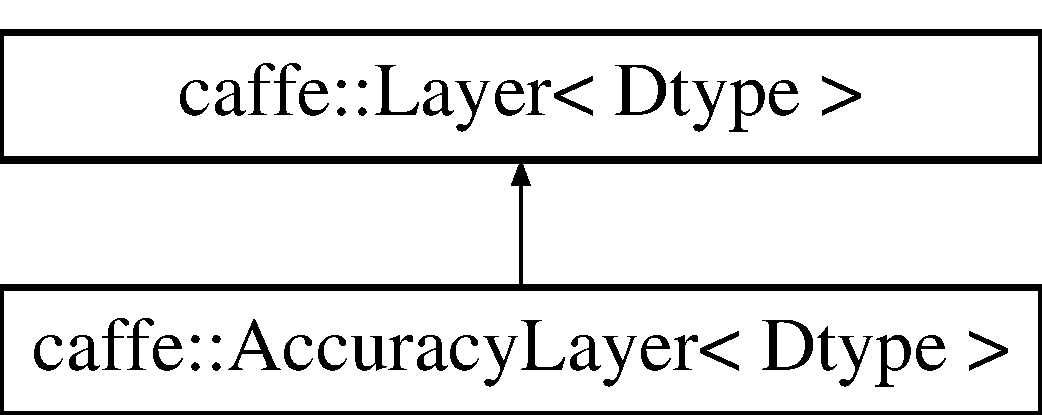
\includegraphics[height=2.000000cm]{classcaffe_1_1_accuracy_layer}
\end{center}
\end{figure}
\subsection*{Public Member Functions}
\begin{DoxyCompactItemize}
\item 
\hyperlink{classcaffe_1_1_accuracy_layer_a362ab61d1961c1b408f84a956f6e598d}{Accuracy\+Layer} (const Layer\+Parameter \&param)
\item 
virtual void \hyperlink{classcaffe_1_1_accuracy_layer_a5c18f1e710a9d59c0180ad2cd6dc4537}{Set\+Up} (const vector$<$ \hyperlink{classcaffe_1_1_blob}{Blob}$<$ Dtype $>$ $\ast$ $>$ \&bottom, vector$<$ \hyperlink{classcaffe_1_1_blob}{Blob}$<$ Dtype $>$ $\ast$ $>$ $\ast$top)
\end{DoxyCompactItemize}
\subsection*{Protected Member Functions}
\begin{DoxyCompactItemize}
\item 
virtual Dtype \hyperlink{classcaffe_1_1_accuracy_layer_a6b009239ed19e1568fda06654af26e39}{Forward\+\_\+cpu} (const vector$<$ \hyperlink{classcaffe_1_1_blob}{Blob}$<$ Dtype $>$ $\ast$ $>$ \&bottom, vector$<$ \hyperlink{classcaffe_1_1_blob}{Blob}$<$ Dtype $>$ $\ast$ $>$ $\ast$top)
\item 
virtual void \hyperlink{classcaffe_1_1_accuracy_layer_a18aff36af82433e25eca1e0de3276d7f}{Backward\+\_\+cpu} (const vector$<$ \hyperlink{classcaffe_1_1_blob}{Blob}$<$ Dtype $>$ $\ast$ $>$ \&top, const bool propagate\+\_\+down, vector$<$ \hyperlink{classcaffe_1_1_blob}{Blob}$<$ Dtype $>$ $\ast$ $>$ $\ast$bottom)
\end{DoxyCompactItemize}
\subsection*{Additional Inherited Members}


\subsection{Constructor \& Destructor Documentation}
\hypertarget{classcaffe_1_1_accuracy_layer_a362ab61d1961c1b408f84a956f6e598d}{\index{caffe\+::\+Accuracy\+Layer@{caffe\+::\+Accuracy\+Layer}!Accuracy\+Layer@{Accuracy\+Layer}}
\index{Accuracy\+Layer@{Accuracy\+Layer}!caffe\+::\+Accuracy\+Layer@{caffe\+::\+Accuracy\+Layer}}
\subsubsection[{Accuracy\+Layer}]{\setlength{\rightskip}{0pt plus 5cm}template$<$typename Dtype $>$ {\bf caffe\+::\+Accuracy\+Layer}$<$ Dtype $>$\+::{\bf Accuracy\+Layer} (
\begin{DoxyParamCaption}
\item[{const Layer\+Parameter \&}]{param}
\end{DoxyParamCaption}
)\hspace{0.3cm}{\ttfamily [inline]}, {\ttfamily [explicit]}}}\label{classcaffe_1_1_accuracy_layer_a362ab61d1961c1b408f84a956f6e598d}


\subsection{Member Function Documentation}
\hypertarget{classcaffe_1_1_accuracy_layer_a18aff36af82433e25eca1e0de3276d7f}{\index{caffe\+::\+Accuracy\+Layer@{caffe\+::\+Accuracy\+Layer}!Backward\+\_\+cpu@{Backward\+\_\+cpu}}
\index{Backward\+\_\+cpu@{Backward\+\_\+cpu}!caffe\+::\+Accuracy\+Layer@{caffe\+::\+Accuracy\+Layer}}
\subsubsection[{Backward\+\_\+cpu}]{\setlength{\rightskip}{0pt plus 5cm}template$<$typename Dtype $>$ virtual void {\bf caffe\+::\+Accuracy\+Layer}$<$ Dtype $>$\+::Backward\+\_\+cpu (
\begin{DoxyParamCaption}
\item[{const vector$<$ {\bf Blob}$<$ Dtype $>$ $\ast$ $>$ \&}]{top, }
\item[{const bool}]{propagate\+\_\+down, }
\item[{vector$<$ {\bf Blob}$<$ Dtype $>$ $\ast$ $>$ $\ast$}]{bottom}
\end{DoxyParamCaption}
)\hspace{0.3cm}{\ttfamily [inline]}, {\ttfamily [protected]}, {\ttfamily [virtual]}}}\label{classcaffe_1_1_accuracy_layer_a18aff36af82433e25eca1e0de3276d7f}


Implements \hyperlink{classcaffe_1_1_layer_ac2d82011d076237c67997f63e7ee4b80}{caffe\+::\+Layer$<$ Dtype $>$}.

\hypertarget{classcaffe_1_1_accuracy_layer_a6b009239ed19e1568fda06654af26e39}{\index{caffe\+::\+Accuracy\+Layer@{caffe\+::\+Accuracy\+Layer}!Forward\+\_\+cpu@{Forward\+\_\+cpu}}
\index{Forward\+\_\+cpu@{Forward\+\_\+cpu}!caffe\+::\+Accuracy\+Layer@{caffe\+::\+Accuracy\+Layer}}
\subsubsection[{Forward\+\_\+cpu}]{\setlength{\rightskip}{0pt plus 5cm}template$<$typename Dtype $>$ Dtype {\bf caffe\+::\+Accuracy\+Layer}$<$ Dtype $>$\+::Forward\+\_\+cpu (
\begin{DoxyParamCaption}
\item[{const vector$<$ {\bf Blob}$<$ Dtype $>$ $\ast$ $>$ \&}]{bottom, }
\item[{vector$<$ {\bf Blob}$<$ Dtype $>$ $\ast$ $>$ $\ast$}]{top}
\end{DoxyParamCaption}
)\hspace{0.3cm}{\ttfamily [protected]}, {\ttfamily [virtual]}}}\label{classcaffe_1_1_accuracy_layer_a6b009239ed19e1568fda06654af26e39}


Implements \hyperlink{classcaffe_1_1_layer_a8f7f61da3b8b3ca7f2394dee33873353}{caffe\+::\+Layer$<$ Dtype $>$}.

\hypertarget{classcaffe_1_1_accuracy_layer_a5c18f1e710a9d59c0180ad2cd6dc4537}{\index{caffe\+::\+Accuracy\+Layer@{caffe\+::\+Accuracy\+Layer}!Set\+Up@{Set\+Up}}
\index{Set\+Up@{Set\+Up}!caffe\+::\+Accuracy\+Layer@{caffe\+::\+Accuracy\+Layer}}
\subsubsection[{Set\+Up}]{\setlength{\rightskip}{0pt plus 5cm}template$<$typename Dtype $>$ void {\bf caffe\+::\+Accuracy\+Layer}$<$ Dtype $>$\+::Set\+Up (
\begin{DoxyParamCaption}
\item[{const vector$<$ {\bf Blob}$<$ Dtype $>$ $\ast$ $>$ \&}]{bottom, }
\item[{vector$<$ {\bf Blob}$<$ Dtype $>$ $\ast$ $>$ $\ast$}]{top}
\end{DoxyParamCaption}
)\hspace{0.3cm}{\ttfamily [virtual]}}}\label{classcaffe_1_1_accuracy_layer_a5c18f1e710a9d59c0180ad2cd6dc4537}


Implements \hyperlink{classcaffe_1_1_layer_abd13c6489c13953b4fbcfcf6880835d0}{caffe\+::\+Layer$<$ Dtype $>$}.



The documentation for this class was generated from the following files\+:\begin{DoxyCompactItemize}
\item 
include/caffe/\hyperlink{vision__layers_8hpp}{vision\+\_\+layers.\+hpp}\item 
src/caffe/layers/\hyperlink{loss__layer_8cpp}{loss\+\_\+layer.\+cpp}\end{DoxyCompactItemize}

\hypertarget{classcaffe_1_1_benchmark_test}{\section{caffe\+:\+:Benchmark\+Test Class Reference}
\label{classcaffe_1_1_benchmark_test}\index{caffe\+::\+Benchmark\+Test@{caffe\+::\+Benchmark\+Test}}
}
Inheritance diagram for caffe\+:\+:Benchmark\+Test\+:\begin{figure}[H]
\begin{center}
\leavevmode
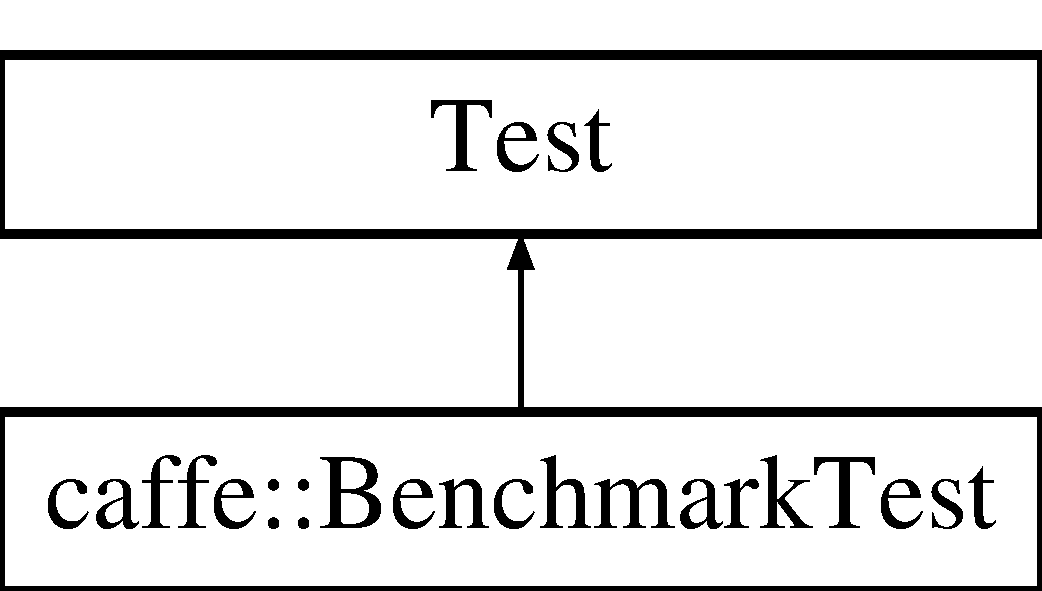
\includegraphics[height=2.000000cm]{classcaffe_1_1_benchmark_test}
\end{center}
\end{figure}


The documentation for this class was generated from the following file\+:\begin{DoxyCompactItemize}
\item 
src/caffe/test/\hyperlink{test__benchmark_8cpp}{test\+\_\+benchmark.\+cpp}\end{DoxyCompactItemize}

\hypertarget{classcaffe_1_1_blob}{\section{caffe\+:\+:Blob$<$ Dtype $>$ Class Template Reference}
\label{classcaffe_1_1_blob}\index{caffe\+::\+Blob$<$ Dtype $>$@{caffe\+::\+Blob$<$ Dtype $>$}}
}


{\ttfamily \#include $<$blob.\+hpp$>$}

\subsection*{Public Member Functions}
\begin{DoxyCompactItemize}
\item 
\hyperlink{classcaffe_1_1_blob_a5ec3bf9e25255c6071db8cfd1dc7f4e9}{Blob} ()
\item 
\hyperlink{classcaffe_1_1_blob_a379df830aad9b3cae253e1ddb0863844}{Blob} (const int \hyperlink{classcaffe_1_1_blob_a56c2b25db397d9e82bbd7c43597ae427}{num}, const int \hyperlink{classcaffe_1_1_blob_a744a987091c4496a2236898ee39558ec}{channels}, const int \hyperlink{classcaffe_1_1_blob_a422a10a605c30ac02a5377e7cf4c8c6c}{height}, const int \hyperlink{classcaffe_1_1_blob_a781b5410b7894455a85cd283cf8ee02a}{width})
\item 
void \hyperlink{classcaffe_1_1_blob_ad0e0a9a4f49478e89161c6afe4e341a0}{Reshape} (const int \hyperlink{classcaffe_1_1_blob_a56c2b25db397d9e82bbd7c43597ae427}{num}, const int \hyperlink{classcaffe_1_1_blob_a744a987091c4496a2236898ee39558ec}{channels}, const int \hyperlink{classcaffe_1_1_blob_a422a10a605c30ac02a5377e7cf4c8c6c}{height}, const int \hyperlink{classcaffe_1_1_blob_a781b5410b7894455a85cd283cf8ee02a}{width})
\item 
void \hyperlink{classcaffe_1_1_blob_aa8dee739aaa4253f73c44904784ce417}{Reshape\+Like} (const \hyperlink{classcaffe_1_1_blob}{Blob} \&other)
\item 
int \hyperlink{classcaffe_1_1_blob_a56c2b25db397d9e82bbd7c43597ae427}{num} () const 
\item 
int \hyperlink{classcaffe_1_1_blob_a744a987091c4496a2236898ee39558ec}{channels} () const 
\item 
int \hyperlink{classcaffe_1_1_blob_a422a10a605c30ac02a5377e7cf4c8c6c}{height} () const 
\item 
int \hyperlink{classcaffe_1_1_blob_a781b5410b7894455a85cd283cf8ee02a}{width} () const 
\item 
int \hyperlink{classcaffe_1_1_blob_abf97753a599dd546c16d55ba926d4e81}{count} () const 
\item 
int \hyperlink{classcaffe_1_1_blob_a87022dfa6cc45b3a2727ccce9ccf4b2c}{offset} (const int n, const int c=0, const int h=0, const int w=0) const 
\item 
void \hyperlink{classcaffe_1_1_blob_a64ad51f99e88233f43a21a85ebe10284}{Copy\+From} (const \hyperlink{classcaffe_1_1_blob}{Blob}$<$ Dtype $>$ \&source, bool copy\+\_\+diff=false, bool reshape=false)
\item 
Dtype \hyperlink{classcaffe_1_1_blob_a3f12332d9d8a0a5adc12c8c75bbbd335}{data\+\_\+at} (const int n, const int c, const int h, const int w) const 
\item 
Dtype \hyperlink{classcaffe_1_1_blob_a349ee9442e5ba9736b6ccf12359e776e}{diff\+\_\+at} (const int n, const int c, const int h, const int w) const 
\item 
const shared\+\_\+ptr$<$ \hyperlink{classcaffe_1_1_synced_memory}{Synced\+Memory} $>$ \& \hyperlink{classcaffe_1_1_blob_a09d1435056f21ba9df52cee4d6371087}{data} () const 
\item 
const shared\+\_\+ptr$<$ \hyperlink{classcaffe_1_1_synced_memory}{Synced\+Memory} $>$ \& \hyperlink{classcaffe_1_1_blob_ab7a8c2034a34695fe5f777ff3271e80d}{diff} () const 
\item 
const Dtype $\ast$ \hyperlink{classcaffe_1_1_blob_a490e0b609d0d62dbfc317cbe76aa8fa2}{cpu\+\_\+data} () const 
\item 
void \hyperlink{classcaffe_1_1_blob_a5d7d38b157e43ff6a8b8bf94b6815daf}{set\+\_\+cpu\+\_\+data} (Dtype $\ast$\hyperlink{classcaffe_1_1_blob_a09d1435056f21ba9df52cee4d6371087}{data})
\item 
const Dtype $\ast$ \hyperlink{classcaffe_1_1_blob_afd60f6fa2044997149075817991bfc19}{gpu\+\_\+data} () const 
\item 
const Dtype $\ast$ \hyperlink{classcaffe_1_1_blob_a59dc87d97e8a0db8302b142eacb64e10}{cpu\+\_\+diff} () const 
\item 
const Dtype $\ast$ \hyperlink{classcaffe_1_1_blob_aafcc1d137ff67dea2d65824ce67bb21d}{gpu\+\_\+diff} () const 
\item 
Dtype $\ast$ \hyperlink{classcaffe_1_1_blob_ac170c040c34e2e78e7fc0d2ee12cf0ef}{mutable\+\_\+cpu\+\_\+data} ()
\item 
Dtype $\ast$ \hyperlink{classcaffe_1_1_blob_abac6bde0521e019df173213af6808e3b}{mutable\+\_\+gpu\+\_\+data} ()
\item 
Dtype $\ast$ \hyperlink{classcaffe_1_1_blob_a4eb870499aa659a5eee7af622cd92eca}{mutable\+\_\+cpu\+\_\+diff} ()
\item 
Dtype $\ast$ \hyperlink{classcaffe_1_1_blob_a8d230bed098a5ee31559df0b8e2db252}{mutable\+\_\+gpu\+\_\+diff} ()
\item 
void \hyperlink{classcaffe_1_1_blob_afe035d7b60c56e4aed2a18296e8ffdc5}{Update} ()
\item 
void \hyperlink{classcaffe_1_1_blob_aa8b8ccc2dc4c68f07b2257d69cb4bc90}{From\+Proto} (const Blob\+Proto \&proto)
\item 
void \hyperlink{classcaffe_1_1_blob_ad297f6b6cad67200c3b5201034653271}{To\+Proto} (Blob\+Proto $\ast$proto, bool write\+\_\+diff=false) const 
\item 
void \hyperlink{classcaffe_1_1_blob_a8fce5a816a2b9629686db69108610d93}{Share\+Data} (const \hyperlink{classcaffe_1_1_blob}{Blob} \&other)
\item 
void \hyperlink{classcaffe_1_1_blob_a004781965b09f94c409cec9a6fc7c35c}{Share\+Diff} (const \hyperlink{classcaffe_1_1_blob}{Blob} \&other)
\end{DoxyCompactItemize}
\subsection*{Protected Member Functions}
\begin{DoxyCompactItemize}
\item 
\hyperlink{classcaffe_1_1_blob_a603f1a5472e5fae9ca8fec62f6d5c581}{D\+I\+S\+A\+B\+L\+E\+\_\+\+C\+O\+P\+Y\+\_\+\+A\+N\+D\+\_\+\+A\+S\+S\+I\+G\+N} (\hyperlink{classcaffe_1_1_blob}{Blob})
\end{DoxyCompactItemize}
\subsection*{Protected Attributes}
\begin{DoxyCompactItemize}
\item 
shared\+\_\+ptr$<$ \hyperlink{classcaffe_1_1_synced_memory}{Synced\+Memory} $>$ \hyperlink{classcaffe_1_1_blob_a5240277a3cea1bc530deca40ca0d0e16}{data\+\_\+}
\item 
shared\+\_\+ptr$<$ \hyperlink{classcaffe_1_1_synced_memory}{Synced\+Memory} $>$ \hyperlink{classcaffe_1_1_blob_a9310f9007aa45e529cb6d69d32dbb80c}{diff\+\_\+}
\item 
int \hyperlink{classcaffe_1_1_blob_a1af8433c8c66ae8f2732aa4d102b6c29}{num\+\_\+}
\item 
int \hyperlink{classcaffe_1_1_blob_a7618f913659955dcee178c00a842065c}{channels\+\_\+}
\item 
int \hyperlink{classcaffe_1_1_blob_ada72205fe499a098a6d17b4b1cd34a82}{height\+\_\+}
\item 
int \hyperlink{classcaffe_1_1_blob_a5ea591a12504b44d94e3715d88fb37a9}{width\+\_\+}
\item 
int \hyperlink{classcaffe_1_1_blob_acf06ea13a3a14f77c178a525c35a3ea0}{count\+\_\+}
\end{DoxyCompactItemize}


\subsection{Constructor \& Destructor Documentation}
\hypertarget{classcaffe_1_1_blob_a5ec3bf9e25255c6071db8cfd1dc7f4e9}{\index{caffe\+::\+Blob@{caffe\+::\+Blob}!Blob@{Blob}}
\index{Blob@{Blob}!caffe\+::\+Blob@{caffe\+::\+Blob}}
\subsubsection[{Blob}]{\setlength{\rightskip}{0pt plus 5cm}template$<$typename Dtype$>$ {\bf caffe\+::\+Blob}$<$ Dtype $>$\+::{\bf Blob} (
\begin{DoxyParamCaption}
{}
\end{DoxyParamCaption}
)\hspace{0.3cm}{\ttfamily [inline]}}}\label{classcaffe_1_1_blob_a5ec3bf9e25255c6071db8cfd1dc7f4e9}
\hypertarget{classcaffe_1_1_blob_a379df830aad9b3cae253e1ddb0863844}{\index{caffe\+::\+Blob@{caffe\+::\+Blob}!Blob@{Blob}}
\index{Blob@{Blob}!caffe\+::\+Blob@{caffe\+::\+Blob}}
\subsubsection[{Blob}]{\setlength{\rightskip}{0pt plus 5cm}template$<$typename Dtype $>$ {\bf caffe\+::\+Blob}$<$ Dtype $>$\+::{\bf Blob} (
\begin{DoxyParamCaption}
\item[{const int}]{num, }
\item[{const int}]{channels, }
\item[{const int}]{height, }
\item[{const int}]{width}
\end{DoxyParamCaption}
)\hspace{0.3cm}{\ttfamily [explicit]}}}\label{classcaffe_1_1_blob_a379df830aad9b3cae253e1ddb0863844}


\subsection{Member Function Documentation}
\hypertarget{classcaffe_1_1_blob_a744a987091c4496a2236898ee39558ec}{\index{caffe\+::\+Blob@{caffe\+::\+Blob}!channels@{channels}}
\index{channels@{channels}!caffe\+::\+Blob@{caffe\+::\+Blob}}
\subsubsection[{channels}]{\setlength{\rightskip}{0pt plus 5cm}template$<$typename Dtype$>$ int {\bf caffe\+::\+Blob}$<$ Dtype $>$\+::channels (
\begin{DoxyParamCaption}
{}
\end{DoxyParamCaption}
) const\hspace{0.3cm}{\ttfamily [inline]}}}\label{classcaffe_1_1_blob_a744a987091c4496a2236898ee39558ec}
\hypertarget{classcaffe_1_1_blob_a64ad51f99e88233f43a21a85ebe10284}{\index{caffe\+::\+Blob@{caffe\+::\+Blob}!Copy\+From@{Copy\+From}}
\index{Copy\+From@{Copy\+From}!caffe\+::\+Blob@{caffe\+::\+Blob}}
\subsubsection[{Copy\+From}]{\setlength{\rightskip}{0pt plus 5cm}template$<$typename Dtype $>$ void {\bf caffe\+::\+Blob}$<$ Dtype $>$\+::Copy\+From (
\begin{DoxyParamCaption}
\item[{const {\bf Blob}$<$ Dtype $>$ \&}]{source, }
\item[{bool}]{copy\+\_\+diff = {\ttfamily false}, }
\item[{bool}]{reshape = {\ttfamily false}}
\end{DoxyParamCaption}
)}}\label{classcaffe_1_1_blob_a64ad51f99e88233f43a21a85ebe10284}
\hypertarget{classcaffe_1_1_blob_abf97753a599dd546c16d55ba926d4e81}{\index{caffe\+::\+Blob@{caffe\+::\+Blob}!count@{count}}
\index{count@{count}!caffe\+::\+Blob@{caffe\+::\+Blob}}
\subsubsection[{count}]{\setlength{\rightskip}{0pt plus 5cm}template$<$typename Dtype$>$ int {\bf caffe\+::\+Blob}$<$ Dtype $>$\+::count (
\begin{DoxyParamCaption}
{}
\end{DoxyParamCaption}
) const\hspace{0.3cm}{\ttfamily [inline]}}}\label{classcaffe_1_1_blob_abf97753a599dd546c16d55ba926d4e81}
\hypertarget{classcaffe_1_1_blob_a490e0b609d0d62dbfc317cbe76aa8fa2}{\index{caffe\+::\+Blob@{caffe\+::\+Blob}!cpu\+\_\+data@{cpu\+\_\+data}}
\index{cpu\+\_\+data@{cpu\+\_\+data}!caffe\+::\+Blob@{caffe\+::\+Blob}}
\subsubsection[{cpu\+\_\+data}]{\setlength{\rightskip}{0pt plus 5cm}template$<$typename Dtype $>$ const Dtype $\ast$ {\bf caffe\+::\+Blob}$<$ Dtype $>$\+::cpu\+\_\+data (
\begin{DoxyParamCaption}
{}
\end{DoxyParamCaption}
) const}}\label{classcaffe_1_1_blob_a490e0b609d0d62dbfc317cbe76aa8fa2}
\hypertarget{classcaffe_1_1_blob_a59dc87d97e8a0db8302b142eacb64e10}{\index{caffe\+::\+Blob@{caffe\+::\+Blob}!cpu\+\_\+diff@{cpu\+\_\+diff}}
\index{cpu\+\_\+diff@{cpu\+\_\+diff}!caffe\+::\+Blob@{caffe\+::\+Blob}}
\subsubsection[{cpu\+\_\+diff}]{\setlength{\rightskip}{0pt plus 5cm}template$<$typename Dtype $>$ const Dtype $\ast$ {\bf caffe\+::\+Blob}$<$ Dtype $>$\+::cpu\+\_\+diff (
\begin{DoxyParamCaption}
{}
\end{DoxyParamCaption}
) const}}\label{classcaffe_1_1_blob_a59dc87d97e8a0db8302b142eacb64e10}
\hypertarget{classcaffe_1_1_blob_a09d1435056f21ba9df52cee4d6371087}{\index{caffe\+::\+Blob@{caffe\+::\+Blob}!data@{data}}
\index{data@{data}!caffe\+::\+Blob@{caffe\+::\+Blob}}
\subsubsection[{data}]{\setlength{\rightskip}{0pt plus 5cm}template$<$typename Dtype$>$ const shared\+\_\+ptr$<${\bf Synced\+Memory}$>$\& {\bf caffe\+::\+Blob}$<$ Dtype $>$\+::data (
\begin{DoxyParamCaption}
{}
\end{DoxyParamCaption}
) const\hspace{0.3cm}{\ttfamily [inline]}}}\label{classcaffe_1_1_blob_a09d1435056f21ba9df52cee4d6371087}
\hypertarget{classcaffe_1_1_blob_a3f12332d9d8a0a5adc12c8c75bbbd335}{\index{caffe\+::\+Blob@{caffe\+::\+Blob}!data\+\_\+at@{data\+\_\+at}}
\index{data\+\_\+at@{data\+\_\+at}!caffe\+::\+Blob@{caffe\+::\+Blob}}
\subsubsection[{data\+\_\+at}]{\setlength{\rightskip}{0pt plus 5cm}template$<$typename Dtype$>$ Dtype {\bf caffe\+::\+Blob}$<$ Dtype $>$\+::data\+\_\+at (
\begin{DoxyParamCaption}
\item[{const int}]{n, }
\item[{const int}]{c, }
\item[{const int}]{h, }
\item[{const int}]{w}
\end{DoxyParamCaption}
) const\hspace{0.3cm}{\ttfamily [inline]}}}\label{classcaffe_1_1_blob_a3f12332d9d8a0a5adc12c8c75bbbd335}
\hypertarget{classcaffe_1_1_blob_ab7a8c2034a34695fe5f777ff3271e80d}{\index{caffe\+::\+Blob@{caffe\+::\+Blob}!diff@{diff}}
\index{diff@{diff}!caffe\+::\+Blob@{caffe\+::\+Blob}}
\subsubsection[{diff}]{\setlength{\rightskip}{0pt plus 5cm}template$<$typename Dtype$>$ const shared\+\_\+ptr$<${\bf Synced\+Memory}$>$\& {\bf caffe\+::\+Blob}$<$ Dtype $>$\+::diff (
\begin{DoxyParamCaption}
{}
\end{DoxyParamCaption}
) const\hspace{0.3cm}{\ttfamily [inline]}}}\label{classcaffe_1_1_blob_ab7a8c2034a34695fe5f777ff3271e80d}
\hypertarget{classcaffe_1_1_blob_a349ee9442e5ba9736b6ccf12359e776e}{\index{caffe\+::\+Blob@{caffe\+::\+Blob}!diff\+\_\+at@{diff\+\_\+at}}
\index{diff\+\_\+at@{diff\+\_\+at}!caffe\+::\+Blob@{caffe\+::\+Blob}}
\subsubsection[{diff\+\_\+at}]{\setlength{\rightskip}{0pt plus 5cm}template$<$typename Dtype$>$ Dtype {\bf caffe\+::\+Blob}$<$ Dtype $>$\+::diff\+\_\+at (
\begin{DoxyParamCaption}
\item[{const int}]{n, }
\item[{const int}]{c, }
\item[{const int}]{h, }
\item[{const int}]{w}
\end{DoxyParamCaption}
) const\hspace{0.3cm}{\ttfamily [inline]}}}\label{classcaffe_1_1_blob_a349ee9442e5ba9736b6ccf12359e776e}
\hypertarget{classcaffe_1_1_blob_a603f1a5472e5fae9ca8fec62f6d5c581}{\index{caffe\+::\+Blob@{caffe\+::\+Blob}!D\+I\+S\+A\+B\+L\+E\+\_\+\+C\+O\+P\+Y\+\_\+\+A\+N\+D\+\_\+\+A\+S\+S\+I\+G\+N@{D\+I\+S\+A\+B\+L\+E\+\_\+\+C\+O\+P\+Y\+\_\+\+A\+N\+D\+\_\+\+A\+S\+S\+I\+G\+N}}
\index{D\+I\+S\+A\+B\+L\+E\+\_\+\+C\+O\+P\+Y\+\_\+\+A\+N\+D\+\_\+\+A\+S\+S\+I\+G\+N@{D\+I\+S\+A\+B\+L\+E\+\_\+\+C\+O\+P\+Y\+\_\+\+A\+N\+D\+\_\+\+A\+S\+S\+I\+G\+N}!caffe\+::\+Blob@{caffe\+::\+Blob}}
\subsubsection[{D\+I\+S\+A\+B\+L\+E\+\_\+\+C\+O\+P\+Y\+\_\+\+A\+N\+D\+\_\+\+A\+S\+S\+I\+G\+N}]{\setlength{\rightskip}{0pt plus 5cm}template$<$typename Dtype$>$ {\bf caffe\+::\+Blob}$<$ Dtype $>$\+::D\+I\+S\+A\+B\+L\+E\+\_\+\+C\+O\+P\+Y\+\_\+\+A\+N\+D\+\_\+\+A\+S\+S\+I\+G\+N (
\begin{DoxyParamCaption}
\item[{{\bf Blob}$<$ Dtype $>$}]{}
\end{DoxyParamCaption}
)\hspace{0.3cm}{\ttfamily [protected]}}}\label{classcaffe_1_1_blob_a603f1a5472e5fae9ca8fec62f6d5c581}
\hypertarget{classcaffe_1_1_blob_aa8b8ccc2dc4c68f07b2257d69cb4bc90}{\index{caffe\+::\+Blob@{caffe\+::\+Blob}!From\+Proto@{From\+Proto}}
\index{From\+Proto@{From\+Proto}!caffe\+::\+Blob@{caffe\+::\+Blob}}
\subsubsection[{From\+Proto}]{\setlength{\rightskip}{0pt plus 5cm}template$<$typename Dtype $>$ void {\bf caffe\+::\+Blob}$<$ Dtype $>$\+::From\+Proto (
\begin{DoxyParamCaption}
\item[{const Blob\+Proto \&}]{proto}
\end{DoxyParamCaption}
)}}\label{classcaffe_1_1_blob_aa8b8ccc2dc4c68f07b2257d69cb4bc90}
\hypertarget{classcaffe_1_1_blob_afd60f6fa2044997149075817991bfc19}{\index{caffe\+::\+Blob@{caffe\+::\+Blob}!gpu\+\_\+data@{gpu\+\_\+data}}
\index{gpu\+\_\+data@{gpu\+\_\+data}!caffe\+::\+Blob@{caffe\+::\+Blob}}
\subsubsection[{gpu\+\_\+data}]{\setlength{\rightskip}{0pt plus 5cm}template$<$typename Dtype $>$ const Dtype $\ast$ {\bf caffe\+::\+Blob}$<$ Dtype $>$\+::gpu\+\_\+data (
\begin{DoxyParamCaption}
{}
\end{DoxyParamCaption}
) const}}\label{classcaffe_1_1_blob_afd60f6fa2044997149075817991bfc19}
\hypertarget{classcaffe_1_1_blob_aafcc1d137ff67dea2d65824ce67bb21d}{\index{caffe\+::\+Blob@{caffe\+::\+Blob}!gpu\+\_\+diff@{gpu\+\_\+diff}}
\index{gpu\+\_\+diff@{gpu\+\_\+diff}!caffe\+::\+Blob@{caffe\+::\+Blob}}
\subsubsection[{gpu\+\_\+diff}]{\setlength{\rightskip}{0pt plus 5cm}template$<$typename Dtype $>$ const Dtype $\ast$ {\bf caffe\+::\+Blob}$<$ Dtype $>$\+::gpu\+\_\+diff (
\begin{DoxyParamCaption}
{}
\end{DoxyParamCaption}
) const}}\label{classcaffe_1_1_blob_aafcc1d137ff67dea2d65824ce67bb21d}
\hypertarget{classcaffe_1_1_blob_a422a10a605c30ac02a5377e7cf4c8c6c}{\index{caffe\+::\+Blob@{caffe\+::\+Blob}!height@{height}}
\index{height@{height}!caffe\+::\+Blob@{caffe\+::\+Blob}}
\subsubsection[{height}]{\setlength{\rightskip}{0pt plus 5cm}template$<$typename Dtype$>$ int {\bf caffe\+::\+Blob}$<$ Dtype $>$\+::height (
\begin{DoxyParamCaption}
{}
\end{DoxyParamCaption}
) const\hspace{0.3cm}{\ttfamily [inline]}}}\label{classcaffe_1_1_blob_a422a10a605c30ac02a5377e7cf4c8c6c}
\hypertarget{classcaffe_1_1_blob_ac170c040c34e2e78e7fc0d2ee12cf0ef}{\index{caffe\+::\+Blob@{caffe\+::\+Blob}!mutable\+\_\+cpu\+\_\+data@{mutable\+\_\+cpu\+\_\+data}}
\index{mutable\+\_\+cpu\+\_\+data@{mutable\+\_\+cpu\+\_\+data}!caffe\+::\+Blob@{caffe\+::\+Blob}}
\subsubsection[{mutable\+\_\+cpu\+\_\+data}]{\setlength{\rightskip}{0pt plus 5cm}template$<$typename Dtype $>$ Dtype $\ast$ {\bf caffe\+::\+Blob}$<$ Dtype $>$\+::mutable\+\_\+cpu\+\_\+data (
\begin{DoxyParamCaption}
{}
\end{DoxyParamCaption}
)}}\label{classcaffe_1_1_blob_ac170c040c34e2e78e7fc0d2ee12cf0ef}
\hypertarget{classcaffe_1_1_blob_a4eb870499aa659a5eee7af622cd92eca}{\index{caffe\+::\+Blob@{caffe\+::\+Blob}!mutable\+\_\+cpu\+\_\+diff@{mutable\+\_\+cpu\+\_\+diff}}
\index{mutable\+\_\+cpu\+\_\+diff@{mutable\+\_\+cpu\+\_\+diff}!caffe\+::\+Blob@{caffe\+::\+Blob}}
\subsubsection[{mutable\+\_\+cpu\+\_\+diff}]{\setlength{\rightskip}{0pt plus 5cm}template$<$typename Dtype $>$ Dtype $\ast$ {\bf caffe\+::\+Blob}$<$ Dtype $>$\+::mutable\+\_\+cpu\+\_\+diff (
\begin{DoxyParamCaption}
{}
\end{DoxyParamCaption}
)}}\label{classcaffe_1_1_blob_a4eb870499aa659a5eee7af622cd92eca}
\hypertarget{classcaffe_1_1_blob_abac6bde0521e019df173213af6808e3b}{\index{caffe\+::\+Blob@{caffe\+::\+Blob}!mutable\+\_\+gpu\+\_\+data@{mutable\+\_\+gpu\+\_\+data}}
\index{mutable\+\_\+gpu\+\_\+data@{mutable\+\_\+gpu\+\_\+data}!caffe\+::\+Blob@{caffe\+::\+Blob}}
\subsubsection[{mutable\+\_\+gpu\+\_\+data}]{\setlength{\rightskip}{0pt plus 5cm}template$<$typename Dtype $>$ Dtype $\ast$ {\bf caffe\+::\+Blob}$<$ Dtype $>$\+::mutable\+\_\+gpu\+\_\+data (
\begin{DoxyParamCaption}
{}
\end{DoxyParamCaption}
)}}\label{classcaffe_1_1_blob_abac6bde0521e019df173213af6808e3b}
\hypertarget{classcaffe_1_1_blob_a8d230bed098a5ee31559df0b8e2db252}{\index{caffe\+::\+Blob@{caffe\+::\+Blob}!mutable\+\_\+gpu\+\_\+diff@{mutable\+\_\+gpu\+\_\+diff}}
\index{mutable\+\_\+gpu\+\_\+diff@{mutable\+\_\+gpu\+\_\+diff}!caffe\+::\+Blob@{caffe\+::\+Blob}}
\subsubsection[{mutable\+\_\+gpu\+\_\+diff}]{\setlength{\rightskip}{0pt plus 5cm}template$<$typename Dtype $>$ Dtype $\ast$ {\bf caffe\+::\+Blob}$<$ Dtype $>$\+::mutable\+\_\+gpu\+\_\+diff (
\begin{DoxyParamCaption}
{}
\end{DoxyParamCaption}
)}}\label{classcaffe_1_1_blob_a8d230bed098a5ee31559df0b8e2db252}
\hypertarget{classcaffe_1_1_blob_a56c2b25db397d9e82bbd7c43597ae427}{\index{caffe\+::\+Blob@{caffe\+::\+Blob}!num@{num}}
\index{num@{num}!caffe\+::\+Blob@{caffe\+::\+Blob}}
\subsubsection[{num}]{\setlength{\rightskip}{0pt plus 5cm}template$<$typename Dtype$>$ int {\bf caffe\+::\+Blob}$<$ Dtype $>$\+::num (
\begin{DoxyParamCaption}
{}
\end{DoxyParamCaption}
) const\hspace{0.3cm}{\ttfamily [inline]}}}\label{classcaffe_1_1_blob_a56c2b25db397d9e82bbd7c43597ae427}
\hypertarget{classcaffe_1_1_blob_a87022dfa6cc45b3a2727ccce9ccf4b2c}{\index{caffe\+::\+Blob@{caffe\+::\+Blob}!offset@{offset}}
\index{offset@{offset}!caffe\+::\+Blob@{caffe\+::\+Blob}}
\subsubsection[{offset}]{\setlength{\rightskip}{0pt plus 5cm}template$<$typename Dtype$>$ int {\bf caffe\+::\+Blob}$<$ Dtype $>$\+::offset (
\begin{DoxyParamCaption}
\item[{const int}]{n, }
\item[{const int}]{c = {\ttfamily 0}, }
\item[{const int}]{h = {\ttfamily 0}, }
\item[{const int}]{w = {\ttfamily 0}}
\end{DoxyParamCaption}
) const\hspace{0.3cm}{\ttfamily [inline]}}}\label{classcaffe_1_1_blob_a87022dfa6cc45b3a2727ccce9ccf4b2c}
\hypertarget{classcaffe_1_1_blob_ad0e0a9a4f49478e89161c6afe4e341a0}{\index{caffe\+::\+Blob@{caffe\+::\+Blob}!Reshape@{Reshape}}
\index{Reshape@{Reshape}!caffe\+::\+Blob@{caffe\+::\+Blob}}
\subsubsection[{Reshape}]{\setlength{\rightskip}{0pt plus 5cm}template$<$typename Dtype $>$ void {\bf caffe\+::\+Blob}$<$ Dtype $>$\+::Reshape (
\begin{DoxyParamCaption}
\item[{const int}]{num, }
\item[{const int}]{channels, }
\item[{const int}]{height, }
\item[{const int}]{width}
\end{DoxyParamCaption}
)}}\label{classcaffe_1_1_blob_ad0e0a9a4f49478e89161c6afe4e341a0}
\hypertarget{classcaffe_1_1_blob_aa8dee739aaa4253f73c44904784ce417}{\index{caffe\+::\+Blob@{caffe\+::\+Blob}!Reshape\+Like@{Reshape\+Like}}
\index{Reshape\+Like@{Reshape\+Like}!caffe\+::\+Blob@{caffe\+::\+Blob}}
\subsubsection[{Reshape\+Like}]{\setlength{\rightskip}{0pt plus 5cm}template$<$typename Dtype $>$ void {\bf caffe\+::\+Blob}$<$ Dtype $>$\+::Reshape\+Like (
\begin{DoxyParamCaption}
\item[{const {\bf Blob}$<$ Dtype $>$ \&}]{other}
\end{DoxyParamCaption}
)}}\label{classcaffe_1_1_blob_aa8dee739aaa4253f73c44904784ce417}
\hypertarget{classcaffe_1_1_blob_a5d7d38b157e43ff6a8b8bf94b6815daf}{\index{caffe\+::\+Blob@{caffe\+::\+Blob}!set\+\_\+cpu\+\_\+data@{set\+\_\+cpu\+\_\+data}}
\index{set\+\_\+cpu\+\_\+data@{set\+\_\+cpu\+\_\+data}!caffe\+::\+Blob@{caffe\+::\+Blob}}
\subsubsection[{set\+\_\+cpu\+\_\+data}]{\setlength{\rightskip}{0pt plus 5cm}template$<$typename Dtype $>$ void {\bf caffe\+::\+Blob}$<$ Dtype $>$\+::set\+\_\+cpu\+\_\+data (
\begin{DoxyParamCaption}
\item[{Dtype $\ast$}]{data}
\end{DoxyParamCaption}
)}}\label{classcaffe_1_1_blob_a5d7d38b157e43ff6a8b8bf94b6815daf}
\hypertarget{classcaffe_1_1_blob_a8fce5a816a2b9629686db69108610d93}{\index{caffe\+::\+Blob@{caffe\+::\+Blob}!Share\+Data@{Share\+Data}}
\index{Share\+Data@{Share\+Data}!caffe\+::\+Blob@{caffe\+::\+Blob}}
\subsubsection[{Share\+Data}]{\setlength{\rightskip}{0pt plus 5cm}template$<$typename Dtype $>$ void {\bf caffe\+::\+Blob}$<$ Dtype $>$\+::Share\+Data (
\begin{DoxyParamCaption}
\item[{const {\bf Blob}$<$ Dtype $>$ \&}]{other}
\end{DoxyParamCaption}
)}}\label{classcaffe_1_1_blob_a8fce5a816a2b9629686db69108610d93}
\hypertarget{classcaffe_1_1_blob_a004781965b09f94c409cec9a6fc7c35c}{\index{caffe\+::\+Blob@{caffe\+::\+Blob}!Share\+Diff@{Share\+Diff}}
\index{Share\+Diff@{Share\+Diff}!caffe\+::\+Blob@{caffe\+::\+Blob}}
\subsubsection[{Share\+Diff}]{\setlength{\rightskip}{0pt plus 5cm}template$<$typename Dtype $>$ void {\bf caffe\+::\+Blob}$<$ Dtype $>$\+::Share\+Diff (
\begin{DoxyParamCaption}
\item[{const {\bf Blob}$<$ Dtype $>$ \&}]{other}
\end{DoxyParamCaption}
)}}\label{classcaffe_1_1_blob_a004781965b09f94c409cec9a6fc7c35c}
\hypertarget{classcaffe_1_1_blob_ad297f6b6cad67200c3b5201034653271}{\index{caffe\+::\+Blob@{caffe\+::\+Blob}!To\+Proto@{To\+Proto}}
\index{To\+Proto@{To\+Proto}!caffe\+::\+Blob@{caffe\+::\+Blob}}
\subsubsection[{To\+Proto}]{\setlength{\rightskip}{0pt plus 5cm}template$<$typename Dtype $>$ void {\bf caffe\+::\+Blob}$<$ Dtype $>$\+::To\+Proto (
\begin{DoxyParamCaption}
\item[{Blob\+Proto $\ast$}]{proto, }
\item[{bool}]{write\+\_\+diff = {\ttfamily false}}
\end{DoxyParamCaption}
) const}}\label{classcaffe_1_1_blob_ad297f6b6cad67200c3b5201034653271}
\hypertarget{classcaffe_1_1_blob_afe035d7b60c56e4aed2a18296e8ffdc5}{\index{caffe\+::\+Blob@{caffe\+::\+Blob}!Update@{Update}}
\index{Update@{Update}!caffe\+::\+Blob@{caffe\+::\+Blob}}
\subsubsection[{Update}]{\setlength{\rightskip}{0pt plus 5cm}template$<$typename Dtype $>$ void {\bf caffe\+::\+Blob}$<$ Dtype $>$\+::Update (
\begin{DoxyParamCaption}
{}
\end{DoxyParamCaption}
)}}\label{classcaffe_1_1_blob_afe035d7b60c56e4aed2a18296e8ffdc5}
\hypertarget{classcaffe_1_1_blob_a781b5410b7894455a85cd283cf8ee02a}{\index{caffe\+::\+Blob@{caffe\+::\+Blob}!width@{width}}
\index{width@{width}!caffe\+::\+Blob@{caffe\+::\+Blob}}
\subsubsection[{width}]{\setlength{\rightskip}{0pt plus 5cm}template$<$typename Dtype$>$ int {\bf caffe\+::\+Blob}$<$ Dtype $>$\+::width (
\begin{DoxyParamCaption}
{}
\end{DoxyParamCaption}
) const\hspace{0.3cm}{\ttfamily [inline]}}}\label{classcaffe_1_1_blob_a781b5410b7894455a85cd283cf8ee02a}


\subsection{Member Data Documentation}
\hypertarget{classcaffe_1_1_blob_a7618f913659955dcee178c00a842065c}{\index{caffe\+::\+Blob@{caffe\+::\+Blob}!channels\+\_\+@{channels\+\_\+}}
\index{channels\+\_\+@{channels\+\_\+}!caffe\+::\+Blob@{caffe\+::\+Blob}}
\subsubsection[{channels\+\_\+}]{\setlength{\rightskip}{0pt plus 5cm}template$<$typename Dtype$>$ int {\bf caffe\+::\+Blob}$<$ Dtype $>$\+::channels\+\_\+\hspace{0.3cm}{\ttfamily [protected]}}}\label{classcaffe_1_1_blob_a7618f913659955dcee178c00a842065c}
\hypertarget{classcaffe_1_1_blob_acf06ea13a3a14f77c178a525c35a3ea0}{\index{caffe\+::\+Blob@{caffe\+::\+Blob}!count\+\_\+@{count\+\_\+}}
\index{count\+\_\+@{count\+\_\+}!caffe\+::\+Blob@{caffe\+::\+Blob}}
\subsubsection[{count\+\_\+}]{\setlength{\rightskip}{0pt plus 5cm}template$<$typename Dtype$>$ int {\bf caffe\+::\+Blob}$<$ Dtype $>$\+::count\+\_\+\hspace{0.3cm}{\ttfamily [protected]}}}\label{classcaffe_1_1_blob_acf06ea13a3a14f77c178a525c35a3ea0}
\hypertarget{classcaffe_1_1_blob_a5240277a3cea1bc530deca40ca0d0e16}{\index{caffe\+::\+Blob@{caffe\+::\+Blob}!data\+\_\+@{data\+\_\+}}
\index{data\+\_\+@{data\+\_\+}!caffe\+::\+Blob@{caffe\+::\+Blob}}
\subsubsection[{data\+\_\+}]{\setlength{\rightskip}{0pt plus 5cm}template$<$typename Dtype$>$ shared\+\_\+ptr$<${\bf Synced\+Memory}$>$ {\bf caffe\+::\+Blob}$<$ Dtype $>$\+::data\+\_\+\hspace{0.3cm}{\ttfamily [protected]}}}\label{classcaffe_1_1_blob_a5240277a3cea1bc530deca40ca0d0e16}
\hypertarget{classcaffe_1_1_blob_a9310f9007aa45e529cb6d69d32dbb80c}{\index{caffe\+::\+Blob@{caffe\+::\+Blob}!diff\+\_\+@{diff\+\_\+}}
\index{diff\+\_\+@{diff\+\_\+}!caffe\+::\+Blob@{caffe\+::\+Blob}}
\subsubsection[{diff\+\_\+}]{\setlength{\rightskip}{0pt plus 5cm}template$<$typename Dtype$>$ shared\+\_\+ptr$<${\bf Synced\+Memory}$>$ {\bf caffe\+::\+Blob}$<$ Dtype $>$\+::diff\+\_\+\hspace{0.3cm}{\ttfamily [protected]}}}\label{classcaffe_1_1_blob_a9310f9007aa45e529cb6d69d32dbb80c}
\hypertarget{classcaffe_1_1_blob_ada72205fe499a098a6d17b4b1cd34a82}{\index{caffe\+::\+Blob@{caffe\+::\+Blob}!height\+\_\+@{height\+\_\+}}
\index{height\+\_\+@{height\+\_\+}!caffe\+::\+Blob@{caffe\+::\+Blob}}
\subsubsection[{height\+\_\+}]{\setlength{\rightskip}{0pt plus 5cm}template$<$typename Dtype$>$ int {\bf caffe\+::\+Blob}$<$ Dtype $>$\+::height\+\_\+\hspace{0.3cm}{\ttfamily [protected]}}}\label{classcaffe_1_1_blob_ada72205fe499a098a6d17b4b1cd34a82}
\hypertarget{classcaffe_1_1_blob_a1af8433c8c66ae8f2732aa4d102b6c29}{\index{caffe\+::\+Blob@{caffe\+::\+Blob}!num\+\_\+@{num\+\_\+}}
\index{num\+\_\+@{num\+\_\+}!caffe\+::\+Blob@{caffe\+::\+Blob}}
\subsubsection[{num\+\_\+}]{\setlength{\rightskip}{0pt plus 5cm}template$<$typename Dtype$>$ int {\bf caffe\+::\+Blob}$<$ Dtype $>$\+::num\+\_\+\hspace{0.3cm}{\ttfamily [protected]}}}\label{classcaffe_1_1_blob_a1af8433c8c66ae8f2732aa4d102b6c29}
\hypertarget{classcaffe_1_1_blob_a5ea591a12504b44d94e3715d88fb37a9}{\index{caffe\+::\+Blob@{caffe\+::\+Blob}!width\+\_\+@{width\+\_\+}}
\index{width\+\_\+@{width\+\_\+}!caffe\+::\+Blob@{caffe\+::\+Blob}}
\subsubsection[{width\+\_\+}]{\setlength{\rightskip}{0pt plus 5cm}template$<$typename Dtype$>$ int {\bf caffe\+::\+Blob}$<$ Dtype $>$\+::width\+\_\+\hspace{0.3cm}{\ttfamily [protected]}}}\label{classcaffe_1_1_blob_a5ea591a12504b44d94e3715d88fb37a9}


The documentation for this class was generated from the following files\+:\begin{DoxyCompactItemize}
\item 
include/caffe/\hyperlink{blob_8hpp}{blob.\+hpp}\item 
src/caffe/\hyperlink{blob_8cpp}{blob.\+cpp}\end{DoxyCompactItemize}

\hypertarget{classcaffe_1_1_blob_simple_test}{\section{caffe\+:\+:Blob\+Simple\+Test$<$ Dtype $>$ Class Template Reference}
\label{classcaffe_1_1_blob_simple_test}\index{caffe\+::\+Blob\+Simple\+Test$<$ Dtype $>$@{caffe\+::\+Blob\+Simple\+Test$<$ Dtype $>$}}
}
Inheritance diagram for caffe\+:\+:Blob\+Simple\+Test$<$ Dtype $>$\+:\begin{figure}[H]
\begin{center}
\leavevmode
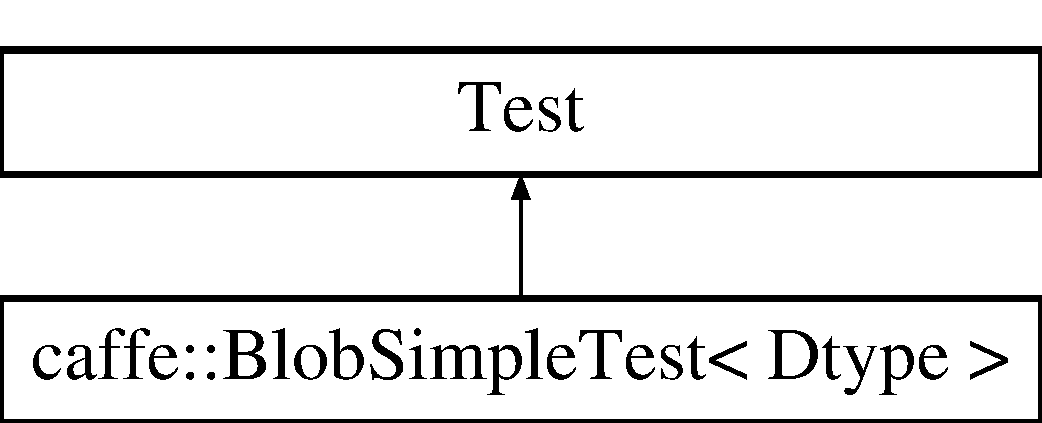
\includegraphics[height=2.000000cm]{classcaffe_1_1_blob_simple_test}
\end{center}
\end{figure}
\subsection*{Protected Member Functions}
\begin{DoxyCompactItemize}
\item 
\hyperlink{classcaffe_1_1_blob_simple_test_ab5df4d4985aa07d6452e74cfcc7635d9}{Blob\+Simple\+Test} ()
\item 
virtual \hyperlink{classcaffe_1_1_blob_simple_test_afc7c73bd24a7dd3c475b43617276750c}{$\sim$\+Blob\+Simple\+Test} ()
\end{DoxyCompactItemize}
\subsection*{Protected Attributes}
\begin{DoxyCompactItemize}
\item 
\hyperlink{classcaffe_1_1_blob}{Blob}$<$ Dtype $>$ $\ast$const \hyperlink{classcaffe_1_1_blob_simple_test_a3e468873646ed610428bf0736e848fdd}{blob\+\_\+}
\item 
\hyperlink{classcaffe_1_1_blob}{Blob}$<$ Dtype $>$ $\ast$const \hyperlink{classcaffe_1_1_blob_simple_test_a3614f695be135a4414285ce66bc67a20}{blob\+\_\+preshaped\+\_\+}
\end{DoxyCompactItemize}


\subsection{Constructor \& Destructor Documentation}
\hypertarget{classcaffe_1_1_blob_simple_test_ab5df4d4985aa07d6452e74cfcc7635d9}{\index{caffe\+::\+Blob\+Simple\+Test@{caffe\+::\+Blob\+Simple\+Test}!Blob\+Simple\+Test@{Blob\+Simple\+Test}}
\index{Blob\+Simple\+Test@{Blob\+Simple\+Test}!caffe\+::\+Blob\+Simple\+Test@{caffe\+::\+Blob\+Simple\+Test}}
\subsubsection[{Blob\+Simple\+Test}]{\setlength{\rightskip}{0pt plus 5cm}template$<$typename Dtype $>$ {\bf caffe\+::\+Blob\+Simple\+Test}$<$ Dtype $>$\+::{\bf Blob\+Simple\+Test} (
\begin{DoxyParamCaption}
{}
\end{DoxyParamCaption}
)\hspace{0.3cm}{\ttfamily [inline]}, {\ttfamily [protected]}}}\label{classcaffe_1_1_blob_simple_test_ab5df4d4985aa07d6452e74cfcc7635d9}
\hypertarget{classcaffe_1_1_blob_simple_test_afc7c73bd24a7dd3c475b43617276750c}{\index{caffe\+::\+Blob\+Simple\+Test@{caffe\+::\+Blob\+Simple\+Test}!````~Blob\+Simple\+Test@{$\sim$\+Blob\+Simple\+Test}}
\index{````~Blob\+Simple\+Test@{$\sim$\+Blob\+Simple\+Test}!caffe\+::\+Blob\+Simple\+Test@{caffe\+::\+Blob\+Simple\+Test}}
\subsubsection[{$\sim$\+Blob\+Simple\+Test}]{\setlength{\rightskip}{0pt plus 5cm}template$<$typename Dtype $>$ virtual {\bf caffe\+::\+Blob\+Simple\+Test}$<$ Dtype $>$\+::$\sim${\bf Blob\+Simple\+Test} (
\begin{DoxyParamCaption}
{}
\end{DoxyParamCaption}
)\hspace{0.3cm}{\ttfamily [inline]}, {\ttfamily [protected]}, {\ttfamily [virtual]}}}\label{classcaffe_1_1_blob_simple_test_afc7c73bd24a7dd3c475b43617276750c}


\subsection{Member Data Documentation}
\hypertarget{classcaffe_1_1_blob_simple_test_a3e468873646ed610428bf0736e848fdd}{\index{caffe\+::\+Blob\+Simple\+Test@{caffe\+::\+Blob\+Simple\+Test}!blob\+\_\+@{blob\+\_\+}}
\index{blob\+\_\+@{blob\+\_\+}!caffe\+::\+Blob\+Simple\+Test@{caffe\+::\+Blob\+Simple\+Test}}
\subsubsection[{blob\+\_\+}]{\setlength{\rightskip}{0pt plus 5cm}template$<$typename Dtype $>$ {\bf Blob}$<$Dtype$>$$\ast$ const {\bf caffe\+::\+Blob\+Simple\+Test}$<$ Dtype $>$\+::blob\+\_\+\hspace{0.3cm}{\ttfamily [protected]}}}\label{classcaffe_1_1_blob_simple_test_a3e468873646ed610428bf0736e848fdd}
\hypertarget{classcaffe_1_1_blob_simple_test_a3614f695be135a4414285ce66bc67a20}{\index{caffe\+::\+Blob\+Simple\+Test@{caffe\+::\+Blob\+Simple\+Test}!blob\+\_\+preshaped\+\_\+@{blob\+\_\+preshaped\+\_\+}}
\index{blob\+\_\+preshaped\+\_\+@{blob\+\_\+preshaped\+\_\+}!caffe\+::\+Blob\+Simple\+Test@{caffe\+::\+Blob\+Simple\+Test}}
\subsubsection[{blob\+\_\+preshaped\+\_\+}]{\setlength{\rightskip}{0pt plus 5cm}template$<$typename Dtype $>$ {\bf Blob}$<$Dtype$>$$\ast$ const {\bf caffe\+::\+Blob\+Simple\+Test}$<$ Dtype $>$\+::blob\+\_\+preshaped\+\_\+\hspace{0.3cm}{\ttfamily [protected]}}}\label{classcaffe_1_1_blob_simple_test_a3614f695be135a4414285ce66bc67a20}


The documentation for this class was generated from the following file\+:\begin{DoxyCompactItemize}
\item 
src/caffe/test/\hyperlink{test__blob_8cpp}{test\+\_\+blob.\+cpp}\end{DoxyCompactItemize}

\hypertarget{classcaffe_1_1_b_n_l_l_layer}{\section{caffe\+:\+:B\+N\+L\+L\+Layer$<$ Dtype $>$ Class Template Reference}
\label{classcaffe_1_1_b_n_l_l_layer}\index{caffe\+::\+B\+N\+L\+L\+Layer$<$ Dtype $>$@{caffe\+::\+B\+N\+L\+L\+Layer$<$ Dtype $>$}}
}


{\ttfamily \#include $<$vision\+\_\+layers.\+hpp$>$}

Inheritance diagram for caffe\+:\+:B\+N\+L\+L\+Layer$<$ Dtype $>$\+:\begin{figure}[H]
\begin{center}
\leavevmode
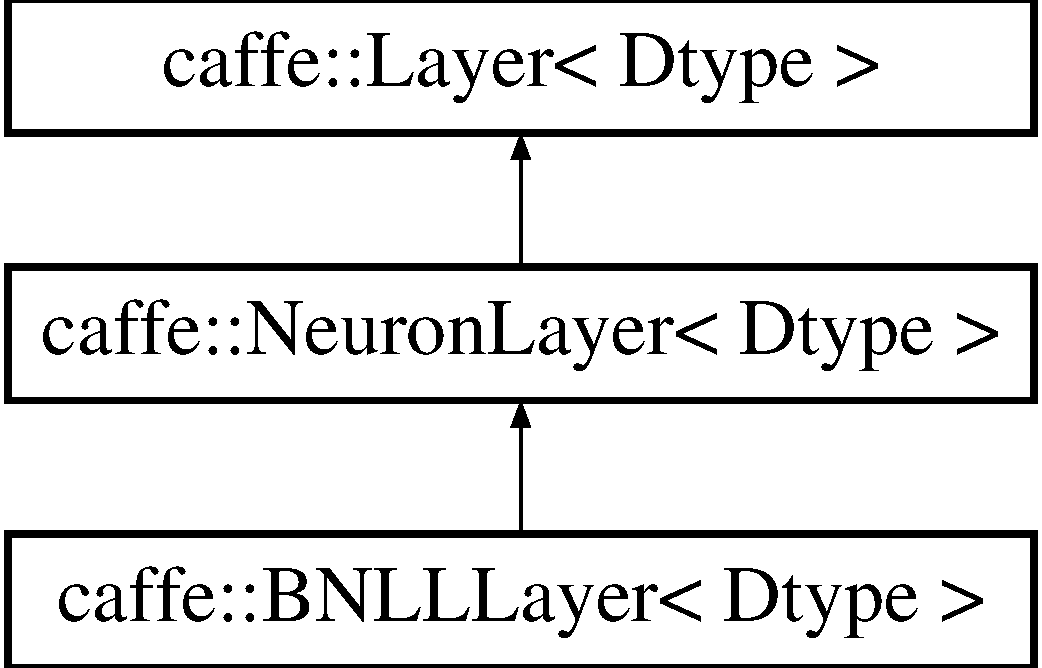
\includegraphics[height=3.000000cm]{classcaffe_1_1_b_n_l_l_layer}
\end{center}
\end{figure}
\subsection*{Public Member Functions}
\begin{DoxyCompactItemize}
\item 
\hyperlink{classcaffe_1_1_b_n_l_l_layer_ab30d4b1d22f7489597449e09d74cf4b9}{B\+N\+L\+L\+Layer} (const Layer\+Parameter \&param)
\end{DoxyCompactItemize}
\subsection*{Protected Member Functions}
\begin{DoxyCompactItemize}
\item 
virtual Dtype \hyperlink{classcaffe_1_1_b_n_l_l_layer_a1a0cb5dd56ad7d93f0d70e93f00263b9}{Forward\+\_\+cpu} (const vector$<$ \hyperlink{classcaffe_1_1_blob}{Blob}$<$ Dtype $>$ $\ast$ $>$ \&bottom, vector$<$ \hyperlink{classcaffe_1_1_blob}{Blob}$<$ Dtype $>$ $\ast$ $>$ $\ast$top)
\item 
virtual Dtype \hyperlink{classcaffe_1_1_b_n_l_l_layer_a880ed4501379ea518a66bc7126b974bc}{Forward\+\_\+gpu} (const vector$<$ \hyperlink{classcaffe_1_1_blob}{Blob}$<$ Dtype $>$ $\ast$ $>$ \&bottom, vector$<$ \hyperlink{classcaffe_1_1_blob}{Blob}$<$ Dtype $>$ $\ast$ $>$ $\ast$top)
\item 
virtual void \hyperlink{classcaffe_1_1_b_n_l_l_layer_acf58b70a8e5fafc303844a822dcf0e3b}{Backward\+\_\+cpu} (const vector$<$ \hyperlink{classcaffe_1_1_blob}{Blob}$<$ Dtype $>$ $\ast$ $>$ \&top, const bool propagate\+\_\+down, vector$<$ \hyperlink{classcaffe_1_1_blob}{Blob}$<$ Dtype $>$ $\ast$ $>$ $\ast$bottom)
\item 
virtual void \hyperlink{classcaffe_1_1_b_n_l_l_layer_a9732b6f05aac77d59e9a906a300b7bfe}{Backward\+\_\+gpu} (const vector$<$ \hyperlink{classcaffe_1_1_blob}{Blob}$<$ Dtype $>$ $\ast$ $>$ \&top, const bool propagate\+\_\+down, vector$<$ \hyperlink{classcaffe_1_1_blob}{Blob}$<$ Dtype $>$ $\ast$ $>$ $\ast$bottom)
\end{DoxyCompactItemize}
\subsection*{Additional Inherited Members}


\subsection{Constructor \& Destructor Documentation}
\hypertarget{classcaffe_1_1_b_n_l_l_layer_ab30d4b1d22f7489597449e09d74cf4b9}{\index{caffe\+::\+B\+N\+L\+L\+Layer@{caffe\+::\+B\+N\+L\+L\+Layer}!B\+N\+L\+L\+Layer@{B\+N\+L\+L\+Layer}}
\index{B\+N\+L\+L\+Layer@{B\+N\+L\+L\+Layer}!caffe\+::\+B\+N\+L\+L\+Layer@{caffe\+::\+B\+N\+L\+L\+Layer}}
\subsubsection[{B\+N\+L\+L\+Layer}]{\setlength{\rightskip}{0pt plus 5cm}template$<$typename Dtype $>$ {\bf caffe\+::\+B\+N\+L\+L\+Layer}$<$ Dtype $>$\+::{\bf B\+N\+L\+L\+Layer} (
\begin{DoxyParamCaption}
\item[{const Layer\+Parameter \&}]{param}
\end{DoxyParamCaption}
)\hspace{0.3cm}{\ttfamily [inline]}, {\ttfamily [explicit]}}}\label{classcaffe_1_1_b_n_l_l_layer_ab30d4b1d22f7489597449e09d74cf4b9}


\subsection{Member Function Documentation}
\hypertarget{classcaffe_1_1_b_n_l_l_layer_acf58b70a8e5fafc303844a822dcf0e3b}{\index{caffe\+::\+B\+N\+L\+L\+Layer@{caffe\+::\+B\+N\+L\+L\+Layer}!Backward\+\_\+cpu@{Backward\+\_\+cpu}}
\index{Backward\+\_\+cpu@{Backward\+\_\+cpu}!caffe\+::\+B\+N\+L\+L\+Layer@{caffe\+::\+B\+N\+L\+L\+Layer}}
\subsubsection[{Backward\+\_\+cpu}]{\setlength{\rightskip}{0pt plus 5cm}template$<$typename Dtype $>$ void {\bf caffe\+::\+B\+N\+L\+L\+Layer}$<$ Dtype $>$\+::Backward\+\_\+cpu (
\begin{DoxyParamCaption}
\item[{const vector$<$ {\bf Blob}$<$ Dtype $>$ $\ast$ $>$ \&}]{top, }
\item[{const bool}]{propagate\+\_\+down, }
\item[{vector$<$ {\bf Blob}$<$ Dtype $>$ $\ast$ $>$ $\ast$}]{bottom}
\end{DoxyParamCaption}
)\hspace{0.3cm}{\ttfamily [protected]}, {\ttfamily [virtual]}}}\label{classcaffe_1_1_b_n_l_l_layer_acf58b70a8e5fafc303844a822dcf0e3b}


Implements \hyperlink{classcaffe_1_1_layer_ac2d82011d076237c67997f63e7ee4b80}{caffe\+::\+Layer$<$ Dtype $>$}.

\hypertarget{classcaffe_1_1_b_n_l_l_layer_a9732b6f05aac77d59e9a906a300b7bfe}{\index{caffe\+::\+B\+N\+L\+L\+Layer@{caffe\+::\+B\+N\+L\+L\+Layer}!Backward\+\_\+gpu@{Backward\+\_\+gpu}}
\index{Backward\+\_\+gpu@{Backward\+\_\+gpu}!caffe\+::\+B\+N\+L\+L\+Layer@{caffe\+::\+B\+N\+L\+L\+Layer}}
\subsubsection[{Backward\+\_\+gpu}]{\setlength{\rightskip}{0pt plus 5cm}template$<$typename Dtype $>$ void {\bf caffe\+::\+B\+N\+L\+L\+Layer}$<$ Dtype $>$\+::Backward\+\_\+gpu (
\begin{DoxyParamCaption}
\item[{const vector$<$ {\bf Blob}$<$ Dtype $>$ $\ast$ $>$ \&}]{top, }
\item[{const bool}]{propagate\+\_\+down, }
\item[{vector$<$ {\bf Blob}$<$ Dtype $>$ $\ast$ $>$ $\ast$}]{bottom}
\end{DoxyParamCaption}
)\hspace{0.3cm}{\ttfamily [protected]}, {\ttfamily [virtual]}}}\label{classcaffe_1_1_b_n_l_l_layer_a9732b6f05aac77d59e9a906a300b7bfe}


Reimplemented from \hyperlink{classcaffe_1_1_layer_adf07ffe1f22d2fd2b1b0ff475ef5a64b}{caffe\+::\+Layer$<$ Dtype $>$}.

\hypertarget{classcaffe_1_1_b_n_l_l_layer_a1a0cb5dd56ad7d93f0d70e93f00263b9}{\index{caffe\+::\+B\+N\+L\+L\+Layer@{caffe\+::\+B\+N\+L\+L\+Layer}!Forward\+\_\+cpu@{Forward\+\_\+cpu}}
\index{Forward\+\_\+cpu@{Forward\+\_\+cpu}!caffe\+::\+B\+N\+L\+L\+Layer@{caffe\+::\+B\+N\+L\+L\+Layer}}
\subsubsection[{Forward\+\_\+cpu}]{\setlength{\rightskip}{0pt plus 5cm}template$<$typename Dtype $>$ Dtype {\bf caffe\+::\+B\+N\+L\+L\+Layer}$<$ Dtype $>$\+::Forward\+\_\+cpu (
\begin{DoxyParamCaption}
\item[{const vector$<$ {\bf Blob}$<$ Dtype $>$ $\ast$ $>$ \&}]{bottom, }
\item[{vector$<$ {\bf Blob}$<$ Dtype $>$ $\ast$ $>$ $\ast$}]{top}
\end{DoxyParamCaption}
)\hspace{0.3cm}{\ttfamily [protected]}, {\ttfamily [virtual]}}}\label{classcaffe_1_1_b_n_l_l_layer_a1a0cb5dd56ad7d93f0d70e93f00263b9}


Implements \hyperlink{classcaffe_1_1_layer_a8f7f61da3b8b3ca7f2394dee33873353}{caffe\+::\+Layer$<$ Dtype $>$}.

\hypertarget{classcaffe_1_1_b_n_l_l_layer_a880ed4501379ea518a66bc7126b974bc}{\index{caffe\+::\+B\+N\+L\+L\+Layer@{caffe\+::\+B\+N\+L\+L\+Layer}!Forward\+\_\+gpu@{Forward\+\_\+gpu}}
\index{Forward\+\_\+gpu@{Forward\+\_\+gpu}!caffe\+::\+B\+N\+L\+L\+Layer@{caffe\+::\+B\+N\+L\+L\+Layer}}
\subsubsection[{Forward\+\_\+gpu}]{\setlength{\rightskip}{0pt plus 5cm}template$<$typename Dtype $>$ Dtype {\bf caffe\+::\+B\+N\+L\+L\+Layer}$<$ Dtype $>$\+::Forward\+\_\+gpu (
\begin{DoxyParamCaption}
\item[{const vector$<$ {\bf Blob}$<$ Dtype $>$ $\ast$ $>$ \&}]{bottom, }
\item[{vector$<$ {\bf Blob}$<$ Dtype $>$ $\ast$ $>$ $\ast$}]{top}
\end{DoxyParamCaption}
)\hspace{0.3cm}{\ttfamily [protected]}, {\ttfamily [virtual]}}}\label{classcaffe_1_1_b_n_l_l_layer_a880ed4501379ea518a66bc7126b974bc}


Reimplemented from \hyperlink{classcaffe_1_1_layer_a2d78dbf5d8bc36928bd8f6fcfbafbcef}{caffe\+::\+Layer$<$ Dtype $>$}.



The documentation for this class was generated from the following files\+:\begin{DoxyCompactItemize}
\item 
include/caffe/\hyperlink{vision__layers_8hpp}{vision\+\_\+layers.\+hpp}\item 
src/caffe/layers/\hyperlink{bnll__layer_8cpp}{bnll\+\_\+layer.\+cpp}\item 
src/caffe/layers/\hyperlink{bnll__layer_8cu}{bnll\+\_\+layer.\+cu}\end{DoxyCompactItemize}

\hypertarget{classcaffe_1_1_caffe}{\section{caffe\+:\+:Caffe Class Reference}
\label{classcaffe_1_1_caffe}\index{caffe\+::\+Caffe@{caffe\+::\+Caffe}}
}


{\ttfamily \#include $<$common.\+hpp$>$}

\subsection*{Classes}
\begin{DoxyCompactItemize}
\item 
class \hyperlink{classcaffe_1_1_caffe_1_1_r_n_g}{R\+N\+G}
\end{DoxyCompactItemize}
\subsection*{Public Types}
\begin{DoxyCompactItemize}
\item 
enum \hyperlink{classcaffe_1_1_caffe_af8f607248c1f212be1f6f1c988d80e4e}{Brew} \{ \hyperlink{classcaffe_1_1_caffe_af8f607248c1f212be1f6f1c988d80e4ea63f3aab774a57c836a8ec3b306caa150}{C\+P\+U}, 
\hyperlink{classcaffe_1_1_caffe_af8f607248c1f212be1f6f1c988d80e4ea1c6fc57b019c260dbb06627208cbaeb8}{G\+P\+U}
 \}
\item 
enum \hyperlink{classcaffe_1_1_caffe_ad2993dccc4a615c39259ed7f0d0e24e9}{Phase} \{ \hyperlink{classcaffe_1_1_caffe_ad2993dccc4a615c39259ed7f0d0e24e9a52f1a7dbb49529ada6072caad00a0e5f}{T\+R\+A\+I\+N}, 
\hyperlink{classcaffe_1_1_caffe_ad2993dccc4a615c39259ed7f0d0e24e9acebef56fe5fe2d711e43fe18e779e116}{T\+E\+S\+T}
 \}
\end{DoxyCompactItemize}
\subsection*{Public Member Functions}
\begin{DoxyCompactItemize}
\item 
\hyperlink{classcaffe_1_1_caffe_a5b6a1c6daa535212b43ee7ad23942963}{$\sim$\+Caffe} ()
\end{DoxyCompactItemize}
\subsection*{Static Public Member Functions}
\begin{DoxyCompactItemize}
\item 
static \hyperlink{classcaffe_1_1_caffe}{Caffe} \& \hyperlink{classcaffe_1_1_caffe_a6a0a8e4ff537a038707f50f28f6ca65d}{Get} ()
\item 
static \hyperlink{classcaffe_1_1_caffe_1_1_r_n_g}{R\+N\+G} \& \hyperlink{classcaffe_1_1_caffe_aff31f4285d99f4254e2af4e40678bf5e}{rng\+\_\+stream} ()
\item 
static cublas\+Handle\+\_\+t \hyperlink{classcaffe_1_1_caffe_afbba8bb2af70b628eca89269b81c915f}{cublas\+\_\+handle} ()
\item 
static curand\+Generator\+\_\+t \hyperlink{classcaffe_1_1_caffe_a659f92f48f20d95c46c6629574a26c0f}{curand\+\_\+generator} ()
\item 
static \hyperlink{classcaffe_1_1_caffe_af8f607248c1f212be1f6f1c988d80e4e}{Brew} \hyperlink{classcaffe_1_1_caffe_aa45214769b727ecd971e0d5ed8ffe96a}{mode} ()
\item 
static \hyperlink{classcaffe_1_1_caffe_ad2993dccc4a615c39259ed7f0d0e24e9}{Phase} \hyperlink{classcaffe_1_1_caffe_aa2727a8d4f9290dd2a750590a9c0ad08}{phase} ()
\item 
static void \hyperlink{classcaffe_1_1_caffe_a025008ff5854ba15e62138c81b7a140d}{set\+\_\+mode} (\hyperlink{classcaffe_1_1_caffe_af8f607248c1f212be1f6f1c988d80e4e}{Brew} \hyperlink{classcaffe_1_1_caffe_aa45214769b727ecd971e0d5ed8ffe96a}{mode})
\item 
static void \hyperlink{classcaffe_1_1_caffe_ad1b7dfdc899fda430750adc24aca34f8}{set\+\_\+phase} (\hyperlink{classcaffe_1_1_caffe_ad2993dccc4a615c39259ed7f0d0e24e9}{Phase} \hyperlink{classcaffe_1_1_caffe_aa2727a8d4f9290dd2a750590a9c0ad08}{phase})
\item 
static void \hyperlink{classcaffe_1_1_caffe_a1f6f560b0f9f73a596284908ee44ecc7}{set\+\_\+random\+\_\+seed} (const unsigned int seed)
\item 
static void \hyperlink{classcaffe_1_1_caffe_ac95c04832bf528acb3ae8f1ffa5b6c11}{Set\+Device} (const int device\+\_\+id)
\item 
static void \hyperlink{classcaffe_1_1_caffe_a4af30f25dc929f2b9c1f195e1683a411}{Device\+Query} ()
\end{DoxyCompactItemize}
\subsection*{Protected Attributes}
\begin{DoxyCompactItemize}
\item 
cublas\+Handle\+\_\+t \hyperlink{classcaffe_1_1_caffe_a5fb5298203759722a061644b508ddaeb}{cublas\+\_\+handle\+\_\+}
\item 
curand\+Generator\+\_\+t \hyperlink{classcaffe_1_1_caffe_a0d920ccea7282d5d88335847c0e9ca9e}{curand\+\_\+generator\+\_\+}
\item 
shared\+\_\+ptr$<$ \hyperlink{classcaffe_1_1_caffe_1_1_r_n_g}{R\+N\+G} $>$ \hyperlink{classcaffe_1_1_caffe_a0c1d6159f6add0ae470af9a09836d979}{random\+\_\+generator\+\_\+}
\item 
\hyperlink{classcaffe_1_1_caffe_af8f607248c1f212be1f6f1c988d80e4e}{Brew} \hyperlink{classcaffe_1_1_caffe_aef998c6b69827060630e21a8ccf8884e}{mode\+\_\+}
\item 
\hyperlink{classcaffe_1_1_caffe_ad2993dccc4a615c39259ed7f0d0e24e9}{Phase} \hyperlink{classcaffe_1_1_caffe_ad919ccd26b71547e009bac6debfcc05a}{phase\+\_\+}
\end{DoxyCompactItemize}
\subsection*{Static Protected Attributes}
\begin{DoxyCompactItemize}
\item 
static shared\+\_\+ptr$<$ \hyperlink{classcaffe_1_1_caffe}{Caffe} $>$ \hyperlink{classcaffe_1_1_caffe_a74e06bec4b81b15e2064a216f33467b6}{singleton\+\_\+}
\end{DoxyCompactItemize}


\subsection{Member Enumeration Documentation}
\hypertarget{classcaffe_1_1_caffe_af8f607248c1f212be1f6f1c988d80e4e}{\index{caffe\+::\+Caffe@{caffe\+::\+Caffe}!Brew@{Brew}}
\index{Brew@{Brew}!caffe\+::\+Caffe@{caffe\+::\+Caffe}}
\subsubsection[{Brew}]{\setlength{\rightskip}{0pt plus 5cm}enum {\bf caffe\+::\+Caffe\+::\+Brew}}}\label{classcaffe_1_1_caffe_af8f607248c1f212be1f6f1c988d80e4e}
\begin{Desc}
\item[Enumerator]\par
\begin{description}
\index{C\+P\+U@{C\+P\+U}!caffe\+::\+Caffe@{caffe\+::\+Caffe}}\index{caffe\+::\+Caffe@{caffe\+::\+Caffe}!C\+P\+U@{C\+P\+U}}\item[{\em 
\hypertarget{classcaffe_1_1_caffe_af8f607248c1f212be1f6f1c988d80e4ea63f3aab774a57c836a8ec3b306caa150}{C\+P\+U}\label{classcaffe_1_1_caffe_af8f607248c1f212be1f6f1c988d80e4ea63f3aab774a57c836a8ec3b306caa150}
}]\index{G\+P\+U@{G\+P\+U}!caffe\+::\+Caffe@{caffe\+::\+Caffe}}\index{caffe\+::\+Caffe@{caffe\+::\+Caffe}!G\+P\+U@{G\+P\+U}}\item[{\em 
\hypertarget{classcaffe_1_1_caffe_af8f607248c1f212be1f6f1c988d80e4ea1c6fc57b019c260dbb06627208cbaeb8}{G\+P\+U}\label{classcaffe_1_1_caffe_af8f607248c1f212be1f6f1c988d80e4ea1c6fc57b019c260dbb06627208cbaeb8}
}]\end{description}
\end{Desc}
\hypertarget{classcaffe_1_1_caffe_ad2993dccc4a615c39259ed7f0d0e24e9}{\index{caffe\+::\+Caffe@{caffe\+::\+Caffe}!Phase@{Phase}}
\index{Phase@{Phase}!caffe\+::\+Caffe@{caffe\+::\+Caffe}}
\subsubsection[{Phase}]{\setlength{\rightskip}{0pt plus 5cm}enum {\bf caffe\+::\+Caffe\+::\+Phase}}}\label{classcaffe_1_1_caffe_ad2993dccc4a615c39259ed7f0d0e24e9}
\begin{Desc}
\item[Enumerator]\par
\begin{description}
\index{T\+R\+A\+I\+N@{T\+R\+A\+I\+N}!caffe\+::\+Caffe@{caffe\+::\+Caffe}}\index{caffe\+::\+Caffe@{caffe\+::\+Caffe}!T\+R\+A\+I\+N@{T\+R\+A\+I\+N}}\item[{\em 
\hypertarget{classcaffe_1_1_caffe_ad2993dccc4a615c39259ed7f0d0e24e9a52f1a7dbb49529ada6072caad00a0e5f}{T\+R\+A\+I\+N}\label{classcaffe_1_1_caffe_ad2993dccc4a615c39259ed7f0d0e24e9a52f1a7dbb49529ada6072caad00a0e5f}
}]\index{T\+E\+S\+T@{T\+E\+S\+T}!caffe\+::\+Caffe@{caffe\+::\+Caffe}}\index{caffe\+::\+Caffe@{caffe\+::\+Caffe}!T\+E\+S\+T@{T\+E\+S\+T}}\item[{\em 
\hypertarget{classcaffe_1_1_caffe_ad2993dccc4a615c39259ed7f0d0e24e9acebef56fe5fe2d711e43fe18e779e116}{T\+E\+S\+T}\label{classcaffe_1_1_caffe_ad2993dccc4a615c39259ed7f0d0e24e9acebef56fe5fe2d711e43fe18e779e116}
}]\end{description}
\end{Desc}


\subsection{Constructor \& Destructor Documentation}
\hypertarget{classcaffe_1_1_caffe_a5b6a1c6daa535212b43ee7ad23942963}{\index{caffe\+::\+Caffe@{caffe\+::\+Caffe}!````~Caffe@{$\sim$\+Caffe}}
\index{````~Caffe@{$\sim$\+Caffe}!caffe\+::\+Caffe@{caffe\+::\+Caffe}}
\subsubsection[{$\sim$\+Caffe}]{\setlength{\rightskip}{0pt plus 5cm}caffe\+::\+Caffe\+::$\sim$\+Caffe (
\begin{DoxyParamCaption}
{}
\end{DoxyParamCaption}
)}}\label{classcaffe_1_1_caffe_a5b6a1c6daa535212b43ee7ad23942963}


\subsection{Member Function Documentation}
\hypertarget{classcaffe_1_1_caffe_afbba8bb2af70b628eca89269b81c915f}{\index{caffe\+::\+Caffe@{caffe\+::\+Caffe}!cublas\+\_\+handle@{cublas\+\_\+handle}}
\index{cublas\+\_\+handle@{cublas\+\_\+handle}!caffe\+::\+Caffe@{caffe\+::\+Caffe}}
\subsubsection[{cublas\+\_\+handle}]{\setlength{\rightskip}{0pt plus 5cm}static cublas\+Handle\+\_\+t caffe\+::\+Caffe\+::cublas\+\_\+handle (
\begin{DoxyParamCaption}
{}
\end{DoxyParamCaption}
)\hspace{0.3cm}{\ttfamily [inline]}, {\ttfamily [static]}}}\label{classcaffe_1_1_caffe_afbba8bb2af70b628eca89269b81c915f}
\hypertarget{classcaffe_1_1_caffe_a659f92f48f20d95c46c6629574a26c0f}{\index{caffe\+::\+Caffe@{caffe\+::\+Caffe}!curand\+\_\+generator@{curand\+\_\+generator}}
\index{curand\+\_\+generator@{curand\+\_\+generator}!caffe\+::\+Caffe@{caffe\+::\+Caffe}}
\subsubsection[{curand\+\_\+generator}]{\setlength{\rightskip}{0pt plus 5cm}static curand\+Generator\+\_\+t caffe\+::\+Caffe\+::curand\+\_\+generator (
\begin{DoxyParamCaption}
{}
\end{DoxyParamCaption}
)\hspace{0.3cm}{\ttfamily [inline]}, {\ttfamily [static]}}}\label{classcaffe_1_1_caffe_a659f92f48f20d95c46c6629574a26c0f}
\hypertarget{classcaffe_1_1_caffe_a4af30f25dc929f2b9c1f195e1683a411}{\index{caffe\+::\+Caffe@{caffe\+::\+Caffe}!Device\+Query@{Device\+Query}}
\index{Device\+Query@{Device\+Query}!caffe\+::\+Caffe@{caffe\+::\+Caffe}}
\subsubsection[{Device\+Query}]{\setlength{\rightskip}{0pt plus 5cm}void caffe\+::\+Caffe\+::\+Device\+Query (
\begin{DoxyParamCaption}
{}
\end{DoxyParamCaption}
)\hspace{0.3cm}{\ttfamily [static]}}}\label{classcaffe_1_1_caffe_a4af30f25dc929f2b9c1f195e1683a411}
\hypertarget{classcaffe_1_1_caffe_a6a0a8e4ff537a038707f50f28f6ca65d}{\index{caffe\+::\+Caffe@{caffe\+::\+Caffe}!Get@{Get}}
\index{Get@{Get}!caffe\+::\+Caffe@{caffe\+::\+Caffe}}
\subsubsection[{Get}]{\setlength{\rightskip}{0pt plus 5cm}static {\bf Caffe}\& caffe\+::\+Caffe\+::\+Get (
\begin{DoxyParamCaption}
{}
\end{DoxyParamCaption}
)\hspace{0.3cm}{\ttfamily [inline]}, {\ttfamily [static]}}}\label{classcaffe_1_1_caffe_a6a0a8e4ff537a038707f50f28f6ca65d}
\hypertarget{classcaffe_1_1_caffe_aa45214769b727ecd971e0d5ed8ffe96a}{\index{caffe\+::\+Caffe@{caffe\+::\+Caffe}!mode@{mode}}
\index{mode@{mode}!caffe\+::\+Caffe@{caffe\+::\+Caffe}}
\subsubsection[{mode}]{\setlength{\rightskip}{0pt plus 5cm}static {\bf Brew} caffe\+::\+Caffe\+::mode (
\begin{DoxyParamCaption}
{}
\end{DoxyParamCaption}
)\hspace{0.3cm}{\ttfamily [inline]}, {\ttfamily [static]}}}\label{classcaffe_1_1_caffe_aa45214769b727ecd971e0d5ed8ffe96a}
\hypertarget{classcaffe_1_1_caffe_aa2727a8d4f9290dd2a750590a9c0ad08}{\index{caffe\+::\+Caffe@{caffe\+::\+Caffe}!phase@{phase}}
\index{phase@{phase}!caffe\+::\+Caffe@{caffe\+::\+Caffe}}
\subsubsection[{phase}]{\setlength{\rightskip}{0pt plus 5cm}static {\bf Phase} caffe\+::\+Caffe\+::phase (
\begin{DoxyParamCaption}
{}
\end{DoxyParamCaption}
)\hspace{0.3cm}{\ttfamily [inline]}, {\ttfamily [static]}}}\label{classcaffe_1_1_caffe_aa2727a8d4f9290dd2a750590a9c0ad08}
\hypertarget{classcaffe_1_1_caffe_aff31f4285d99f4254e2af4e40678bf5e}{\index{caffe\+::\+Caffe@{caffe\+::\+Caffe}!rng\+\_\+stream@{rng\+\_\+stream}}
\index{rng\+\_\+stream@{rng\+\_\+stream}!caffe\+::\+Caffe@{caffe\+::\+Caffe}}
\subsubsection[{rng\+\_\+stream}]{\setlength{\rightskip}{0pt plus 5cm}static {\bf R\+N\+G}\& caffe\+::\+Caffe\+::rng\+\_\+stream (
\begin{DoxyParamCaption}
{}
\end{DoxyParamCaption}
)\hspace{0.3cm}{\ttfamily [inline]}, {\ttfamily [static]}}}\label{classcaffe_1_1_caffe_aff31f4285d99f4254e2af4e40678bf5e}
\hypertarget{classcaffe_1_1_caffe_a025008ff5854ba15e62138c81b7a140d}{\index{caffe\+::\+Caffe@{caffe\+::\+Caffe}!set\+\_\+mode@{set\+\_\+mode}}
\index{set\+\_\+mode@{set\+\_\+mode}!caffe\+::\+Caffe@{caffe\+::\+Caffe}}
\subsubsection[{set\+\_\+mode}]{\setlength{\rightskip}{0pt plus 5cm}static void caffe\+::\+Caffe\+::set\+\_\+mode (
\begin{DoxyParamCaption}
\item[{{\bf Brew}}]{mode}
\end{DoxyParamCaption}
)\hspace{0.3cm}{\ttfamily [inline]}, {\ttfamily [static]}}}\label{classcaffe_1_1_caffe_a025008ff5854ba15e62138c81b7a140d}
\hypertarget{classcaffe_1_1_caffe_ad1b7dfdc899fda430750adc24aca34f8}{\index{caffe\+::\+Caffe@{caffe\+::\+Caffe}!set\+\_\+phase@{set\+\_\+phase}}
\index{set\+\_\+phase@{set\+\_\+phase}!caffe\+::\+Caffe@{caffe\+::\+Caffe}}
\subsubsection[{set\+\_\+phase}]{\setlength{\rightskip}{0pt plus 5cm}static void caffe\+::\+Caffe\+::set\+\_\+phase (
\begin{DoxyParamCaption}
\item[{{\bf Phase}}]{phase}
\end{DoxyParamCaption}
)\hspace{0.3cm}{\ttfamily [inline]}, {\ttfamily [static]}}}\label{classcaffe_1_1_caffe_ad1b7dfdc899fda430750adc24aca34f8}
\hypertarget{classcaffe_1_1_caffe_a1f6f560b0f9f73a596284908ee44ecc7}{\index{caffe\+::\+Caffe@{caffe\+::\+Caffe}!set\+\_\+random\+\_\+seed@{set\+\_\+random\+\_\+seed}}
\index{set\+\_\+random\+\_\+seed@{set\+\_\+random\+\_\+seed}!caffe\+::\+Caffe@{caffe\+::\+Caffe}}
\subsubsection[{set\+\_\+random\+\_\+seed}]{\setlength{\rightskip}{0pt plus 5cm}void caffe\+::\+Caffe\+::set\+\_\+random\+\_\+seed (
\begin{DoxyParamCaption}
\item[{const unsigned int}]{seed}
\end{DoxyParamCaption}
)\hspace{0.3cm}{\ttfamily [static]}}}\label{classcaffe_1_1_caffe_a1f6f560b0f9f73a596284908ee44ecc7}
\hypertarget{classcaffe_1_1_caffe_ac95c04832bf528acb3ae8f1ffa5b6c11}{\index{caffe\+::\+Caffe@{caffe\+::\+Caffe}!Set\+Device@{Set\+Device}}
\index{Set\+Device@{Set\+Device}!caffe\+::\+Caffe@{caffe\+::\+Caffe}}
\subsubsection[{Set\+Device}]{\setlength{\rightskip}{0pt plus 5cm}void caffe\+::\+Caffe\+::\+Set\+Device (
\begin{DoxyParamCaption}
\item[{const int}]{device\+\_\+id}
\end{DoxyParamCaption}
)\hspace{0.3cm}{\ttfamily [static]}}}\label{classcaffe_1_1_caffe_ac95c04832bf528acb3ae8f1ffa5b6c11}


\subsection{Member Data Documentation}
\hypertarget{classcaffe_1_1_caffe_a5fb5298203759722a061644b508ddaeb}{\index{caffe\+::\+Caffe@{caffe\+::\+Caffe}!cublas\+\_\+handle\+\_\+@{cublas\+\_\+handle\+\_\+}}
\index{cublas\+\_\+handle\+\_\+@{cublas\+\_\+handle\+\_\+}!caffe\+::\+Caffe@{caffe\+::\+Caffe}}
\subsubsection[{cublas\+\_\+handle\+\_\+}]{\setlength{\rightskip}{0pt plus 5cm}cublas\+Handle\+\_\+t caffe\+::\+Caffe\+::cublas\+\_\+handle\+\_\+\hspace{0.3cm}{\ttfamily [protected]}}}\label{classcaffe_1_1_caffe_a5fb5298203759722a061644b508ddaeb}
\hypertarget{classcaffe_1_1_caffe_a0d920ccea7282d5d88335847c0e9ca9e}{\index{caffe\+::\+Caffe@{caffe\+::\+Caffe}!curand\+\_\+generator\+\_\+@{curand\+\_\+generator\+\_\+}}
\index{curand\+\_\+generator\+\_\+@{curand\+\_\+generator\+\_\+}!caffe\+::\+Caffe@{caffe\+::\+Caffe}}
\subsubsection[{curand\+\_\+generator\+\_\+}]{\setlength{\rightskip}{0pt plus 5cm}curand\+Generator\+\_\+t caffe\+::\+Caffe\+::curand\+\_\+generator\+\_\+\hspace{0.3cm}{\ttfamily [protected]}}}\label{classcaffe_1_1_caffe_a0d920ccea7282d5d88335847c0e9ca9e}
\hypertarget{classcaffe_1_1_caffe_aef998c6b69827060630e21a8ccf8884e}{\index{caffe\+::\+Caffe@{caffe\+::\+Caffe}!mode\+\_\+@{mode\+\_\+}}
\index{mode\+\_\+@{mode\+\_\+}!caffe\+::\+Caffe@{caffe\+::\+Caffe}}
\subsubsection[{mode\+\_\+}]{\setlength{\rightskip}{0pt plus 5cm}{\bf Brew} caffe\+::\+Caffe\+::mode\+\_\+\hspace{0.3cm}{\ttfamily [protected]}}}\label{classcaffe_1_1_caffe_aef998c6b69827060630e21a8ccf8884e}
\hypertarget{classcaffe_1_1_caffe_ad919ccd26b71547e009bac6debfcc05a}{\index{caffe\+::\+Caffe@{caffe\+::\+Caffe}!phase\+\_\+@{phase\+\_\+}}
\index{phase\+\_\+@{phase\+\_\+}!caffe\+::\+Caffe@{caffe\+::\+Caffe}}
\subsubsection[{phase\+\_\+}]{\setlength{\rightskip}{0pt plus 5cm}{\bf Phase} caffe\+::\+Caffe\+::phase\+\_\+\hspace{0.3cm}{\ttfamily [protected]}}}\label{classcaffe_1_1_caffe_ad919ccd26b71547e009bac6debfcc05a}
\hypertarget{classcaffe_1_1_caffe_a0c1d6159f6add0ae470af9a09836d979}{\index{caffe\+::\+Caffe@{caffe\+::\+Caffe}!random\+\_\+generator\+\_\+@{random\+\_\+generator\+\_\+}}
\index{random\+\_\+generator\+\_\+@{random\+\_\+generator\+\_\+}!caffe\+::\+Caffe@{caffe\+::\+Caffe}}
\subsubsection[{random\+\_\+generator\+\_\+}]{\setlength{\rightskip}{0pt plus 5cm}shared\+\_\+ptr$<${\bf R\+N\+G}$>$ caffe\+::\+Caffe\+::random\+\_\+generator\+\_\+\hspace{0.3cm}{\ttfamily [protected]}}}\label{classcaffe_1_1_caffe_a0c1d6159f6add0ae470af9a09836d979}
\hypertarget{classcaffe_1_1_caffe_a74e06bec4b81b15e2064a216f33467b6}{\index{caffe\+::\+Caffe@{caffe\+::\+Caffe}!singleton\+\_\+@{singleton\+\_\+}}
\index{singleton\+\_\+@{singleton\+\_\+}!caffe\+::\+Caffe@{caffe\+::\+Caffe}}
\subsubsection[{singleton\+\_\+}]{\setlength{\rightskip}{0pt plus 5cm}shared\+\_\+ptr$<$ {\bf Caffe} $>$ caffe\+::\+Caffe\+::singleton\+\_\+\hspace{0.3cm}{\ttfamily [static]}, {\ttfamily [protected]}}}\label{classcaffe_1_1_caffe_a74e06bec4b81b15e2064a216f33467b6}


The documentation for this class was generated from the following files\+:\begin{DoxyCompactItemize}
\item 
include/caffe/\hyperlink{common_8hpp}{common.\+hpp}\item 
src/caffe/\hyperlink{common_8cpp}{common.\+cpp}\end{DoxyCompactItemize}

\hypertarget{classcaffe_1_1_common_test}{\section{caffe\+:\+:Common\+Test Class Reference}
\label{classcaffe_1_1_common_test}\index{caffe\+::\+Common\+Test@{caffe\+::\+Common\+Test}}
}
Inheritance diagram for caffe\+:\+:Common\+Test\+:\begin{figure}[H]
\begin{center}
\leavevmode
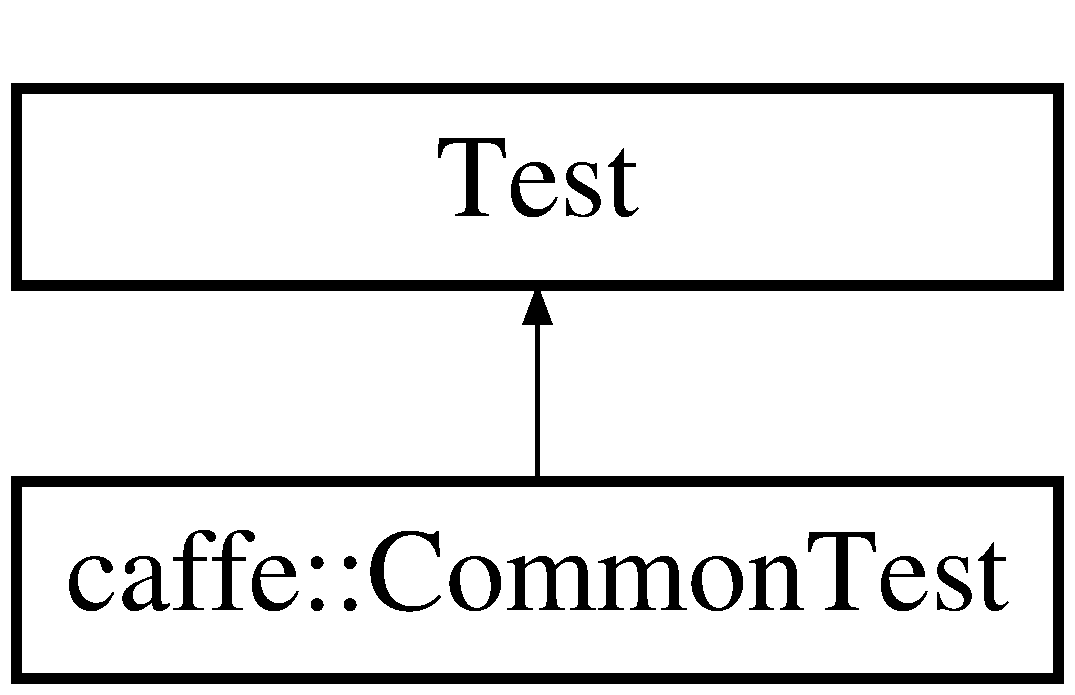
\includegraphics[height=2.000000cm]{classcaffe_1_1_common_test}
\end{center}
\end{figure}


The documentation for this class was generated from the following file\+:\begin{DoxyCompactItemize}
\item 
src/caffe/test/\hyperlink{test__common_8cpp}{test\+\_\+common.\+cpp}\end{DoxyCompactItemize}

\hypertarget{classcaffe_1_1_concat_layer}{\section{caffe\+:\+:Concat\+Layer$<$ Dtype $>$ Class Template Reference}
\label{classcaffe_1_1_concat_layer}\index{caffe\+::\+Concat\+Layer$<$ Dtype $>$@{caffe\+::\+Concat\+Layer$<$ Dtype $>$}}
}


{\ttfamily \#include $<$vision\+\_\+layers.\+hpp$>$}

Inheritance diagram for caffe\+:\+:Concat\+Layer$<$ Dtype $>$\+:\begin{figure}[H]
\begin{center}
\leavevmode
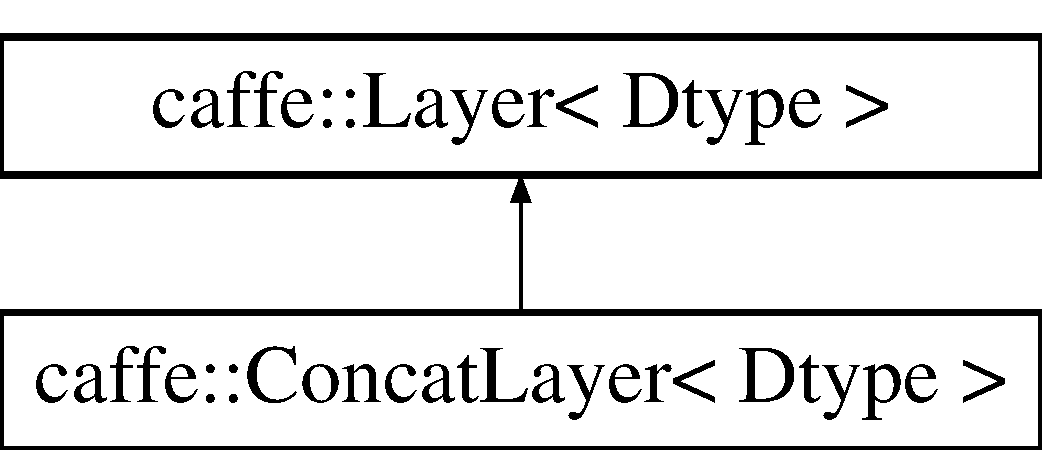
\includegraphics[height=2.000000cm]{classcaffe_1_1_concat_layer}
\end{center}
\end{figure}
\subsection*{Public Member Functions}
\begin{DoxyCompactItemize}
\item 
\hyperlink{classcaffe_1_1_concat_layer_aa06930bae7ed23c88546f35323e1792d}{Concat\+Layer} (const Layer\+Parameter \&param)
\item 
virtual void \hyperlink{classcaffe_1_1_concat_layer_ad479a513d943035c1415309ed61e62d8}{Set\+Up} (const vector$<$ \hyperlink{classcaffe_1_1_blob}{Blob}$<$ Dtype $>$ $\ast$ $>$ \&bottom, vector$<$ \hyperlink{classcaffe_1_1_blob}{Blob}$<$ Dtype $>$ $\ast$ $>$ $\ast$top)
\end{DoxyCompactItemize}
\subsection*{Protected Member Functions}
\begin{DoxyCompactItemize}
\item 
virtual Dtype \hyperlink{classcaffe_1_1_concat_layer_a8d0ef15036059a8b5545c886360148ae}{Forward\+\_\+cpu} (const vector$<$ \hyperlink{classcaffe_1_1_blob}{Blob}$<$ Dtype $>$ $\ast$ $>$ \&bottom, vector$<$ \hyperlink{classcaffe_1_1_blob}{Blob}$<$ Dtype $>$ $\ast$ $>$ $\ast$top)
\item 
virtual Dtype \hyperlink{classcaffe_1_1_concat_layer_a92913d7f28a319354470e56fd306b628}{Forward\+\_\+gpu} (const vector$<$ \hyperlink{classcaffe_1_1_blob}{Blob}$<$ Dtype $>$ $\ast$ $>$ \&bottom, vector$<$ \hyperlink{classcaffe_1_1_blob}{Blob}$<$ Dtype $>$ $\ast$ $>$ $\ast$top)
\item 
virtual void \hyperlink{classcaffe_1_1_concat_layer_ad9f664216981e5f2248cdf88b49c5015}{Backward\+\_\+cpu} (const vector$<$ \hyperlink{classcaffe_1_1_blob}{Blob}$<$ Dtype $>$ $\ast$ $>$ \&top, const bool propagate\+\_\+down, vector$<$ \hyperlink{classcaffe_1_1_blob}{Blob}$<$ Dtype $>$ $\ast$ $>$ $\ast$bottom)
\item 
virtual void \hyperlink{classcaffe_1_1_concat_layer_a86ff8e3cd7ae4f06b23751b60d43ba76}{Backward\+\_\+gpu} (const vector$<$ \hyperlink{classcaffe_1_1_blob}{Blob}$<$ Dtype $>$ $\ast$ $>$ \&top, const bool propagate\+\_\+down, vector$<$ \hyperlink{classcaffe_1_1_blob}{Blob}$<$ Dtype $>$ $\ast$ $>$ $\ast$bottom)
\end{DoxyCompactItemize}
\subsection*{Protected Attributes}
\begin{DoxyCompactItemize}
\item 
\hyperlink{classcaffe_1_1_blob}{Blob}$<$ Dtype $>$ \hyperlink{classcaffe_1_1_concat_layer_a03737f00c69377dd5170c407541d40ff}{col\+\_\+bob\+\_\+}
\item 
int \hyperlink{classcaffe_1_1_concat_layer_a2e8c2179da287e21df345183f431bd72}{count\+\_\+}
\item 
int \hyperlink{classcaffe_1_1_concat_layer_a29dac7e4ccd6c477006551b591269566}{num\+\_\+}
\item 
int \hyperlink{classcaffe_1_1_concat_layer_a5f1ed4b44d327f638b683a6c34348e31}{channels\+\_\+}
\item 
int \hyperlink{classcaffe_1_1_concat_layer_abef01ab0023d78b6df16a7d8e68817c0}{height\+\_\+}
\item 
int \hyperlink{classcaffe_1_1_concat_layer_aae82aa5826cdd79a27c35da49728be4c}{width\+\_\+}
\item 
int \hyperlink{classcaffe_1_1_concat_layer_a85d219531768269ba18f3c331ad94301}{concat\+\_\+dim\+\_\+}
\end{DoxyCompactItemize}


\subsection{Constructor \& Destructor Documentation}
\hypertarget{classcaffe_1_1_concat_layer_aa06930bae7ed23c88546f35323e1792d}{\index{caffe\+::\+Concat\+Layer@{caffe\+::\+Concat\+Layer}!Concat\+Layer@{Concat\+Layer}}
\index{Concat\+Layer@{Concat\+Layer}!caffe\+::\+Concat\+Layer@{caffe\+::\+Concat\+Layer}}
\subsubsection[{Concat\+Layer}]{\setlength{\rightskip}{0pt plus 5cm}template$<$typename Dtype $>$ {\bf caffe\+::\+Concat\+Layer}$<$ Dtype $>$\+::{\bf Concat\+Layer} (
\begin{DoxyParamCaption}
\item[{const Layer\+Parameter \&}]{param}
\end{DoxyParamCaption}
)\hspace{0.3cm}{\ttfamily [inline]}, {\ttfamily [explicit]}}}\label{classcaffe_1_1_concat_layer_aa06930bae7ed23c88546f35323e1792d}


\subsection{Member Function Documentation}
\hypertarget{classcaffe_1_1_concat_layer_ad9f664216981e5f2248cdf88b49c5015}{\index{caffe\+::\+Concat\+Layer@{caffe\+::\+Concat\+Layer}!Backward\+\_\+cpu@{Backward\+\_\+cpu}}
\index{Backward\+\_\+cpu@{Backward\+\_\+cpu}!caffe\+::\+Concat\+Layer@{caffe\+::\+Concat\+Layer}}
\subsubsection[{Backward\+\_\+cpu}]{\setlength{\rightskip}{0pt plus 5cm}template$<$typename Dtype $>$ void {\bf caffe\+::\+Concat\+Layer}$<$ Dtype $>$\+::Backward\+\_\+cpu (
\begin{DoxyParamCaption}
\item[{const vector$<$ {\bf Blob}$<$ Dtype $>$ $\ast$ $>$ \&}]{top, }
\item[{const bool}]{propagate\+\_\+down, }
\item[{vector$<$ {\bf Blob}$<$ Dtype $>$ $\ast$ $>$ $\ast$}]{bottom}
\end{DoxyParamCaption}
)\hspace{0.3cm}{\ttfamily [protected]}, {\ttfamily [virtual]}}}\label{classcaffe_1_1_concat_layer_ad9f664216981e5f2248cdf88b49c5015}


Implements \hyperlink{classcaffe_1_1_layer_ac2d82011d076237c67997f63e7ee4b80}{caffe\+::\+Layer$<$ Dtype $>$}.

\hypertarget{classcaffe_1_1_concat_layer_a86ff8e3cd7ae4f06b23751b60d43ba76}{\index{caffe\+::\+Concat\+Layer@{caffe\+::\+Concat\+Layer}!Backward\+\_\+gpu@{Backward\+\_\+gpu}}
\index{Backward\+\_\+gpu@{Backward\+\_\+gpu}!caffe\+::\+Concat\+Layer@{caffe\+::\+Concat\+Layer}}
\subsubsection[{Backward\+\_\+gpu}]{\setlength{\rightskip}{0pt plus 5cm}template$<$typename Dtype $>$ void {\bf caffe\+::\+Concat\+Layer}$<$ Dtype $>$\+::Backward\+\_\+gpu (
\begin{DoxyParamCaption}
\item[{const vector$<$ {\bf Blob}$<$ Dtype $>$ $\ast$ $>$ \&}]{top, }
\item[{const bool}]{propagate\+\_\+down, }
\item[{vector$<$ {\bf Blob}$<$ Dtype $>$ $\ast$ $>$ $\ast$}]{bottom}
\end{DoxyParamCaption}
)\hspace{0.3cm}{\ttfamily [protected]}, {\ttfamily [virtual]}}}\label{classcaffe_1_1_concat_layer_a86ff8e3cd7ae4f06b23751b60d43ba76}


Reimplemented from \hyperlink{classcaffe_1_1_layer_adf07ffe1f22d2fd2b1b0ff475ef5a64b}{caffe\+::\+Layer$<$ Dtype $>$}.

\hypertarget{classcaffe_1_1_concat_layer_a8d0ef15036059a8b5545c886360148ae}{\index{caffe\+::\+Concat\+Layer@{caffe\+::\+Concat\+Layer}!Forward\+\_\+cpu@{Forward\+\_\+cpu}}
\index{Forward\+\_\+cpu@{Forward\+\_\+cpu}!caffe\+::\+Concat\+Layer@{caffe\+::\+Concat\+Layer}}
\subsubsection[{Forward\+\_\+cpu}]{\setlength{\rightskip}{0pt plus 5cm}template$<$typename Dtype $>$ Dtype {\bf caffe\+::\+Concat\+Layer}$<$ Dtype $>$\+::Forward\+\_\+cpu (
\begin{DoxyParamCaption}
\item[{const vector$<$ {\bf Blob}$<$ Dtype $>$ $\ast$ $>$ \&}]{bottom, }
\item[{vector$<$ {\bf Blob}$<$ Dtype $>$ $\ast$ $>$ $\ast$}]{top}
\end{DoxyParamCaption}
)\hspace{0.3cm}{\ttfamily [protected]}, {\ttfamily [virtual]}}}\label{classcaffe_1_1_concat_layer_a8d0ef15036059a8b5545c886360148ae}


Implements \hyperlink{classcaffe_1_1_layer_a8f7f61da3b8b3ca7f2394dee33873353}{caffe\+::\+Layer$<$ Dtype $>$}.

\hypertarget{classcaffe_1_1_concat_layer_a92913d7f28a319354470e56fd306b628}{\index{caffe\+::\+Concat\+Layer@{caffe\+::\+Concat\+Layer}!Forward\+\_\+gpu@{Forward\+\_\+gpu}}
\index{Forward\+\_\+gpu@{Forward\+\_\+gpu}!caffe\+::\+Concat\+Layer@{caffe\+::\+Concat\+Layer}}
\subsubsection[{Forward\+\_\+gpu}]{\setlength{\rightskip}{0pt plus 5cm}template$<$typename Dtype $>$ Dtype {\bf caffe\+::\+Concat\+Layer}$<$ Dtype $>$\+::Forward\+\_\+gpu (
\begin{DoxyParamCaption}
\item[{const vector$<$ {\bf Blob}$<$ Dtype $>$ $\ast$ $>$ \&}]{bottom, }
\item[{vector$<$ {\bf Blob}$<$ Dtype $>$ $\ast$ $>$ $\ast$}]{top}
\end{DoxyParamCaption}
)\hspace{0.3cm}{\ttfamily [protected]}, {\ttfamily [virtual]}}}\label{classcaffe_1_1_concat_layer_a92913d7f28a319354470e56fd306b628}


Reimplemented from \hyperlink{classcaffe_1_1_layer_a2d78dbf5d8bc36928bd8f6fcfbafbcef}{caffe\+::\+Layer$<$ Dtype $>$}.

\hypertarget{classcaffe_1_1_concat_layer_ad479a513d943035c1415309ed61e62d8}{\index{caffe\+::\+Concat\+Layer@{caffe\+::\+Concat\+Layer}!Set\+Up@{Set\+Up}}
\index{Set\+Up@{Set\+Up}!caffe\+::\+Concat\+Layer@{caffe\+::\+Concat\+Layer}}
\subsubsection[{Set\+Up}]{\setlength{\rightskip}{0pt plus 5cm}template$<$typename Dtype $>$ void {\bf caffe\+::\+Concat\+Layer}$<$ Dtype $>$\+::Set\+Up (
\begin{DoxyParamCaption}
\item[{const vector$<$ {\bf Blob}$<$ Dtype $>$ $\ast$ $>$ \&}]{bottom, }
\item[{vector$<$ {\bf Blob}$<$ Dtype $>$ $\ast$ $>$ $\ast$}]{top}
\end{DoxyParamCaption}
)\hspace{0.3cm}{\ttfamily [virtual]}}}\label{classcaffe_1_1_concat_layer_ad479a513d943035c1415309ed61e62d8}


Implements \hyperlink{classcaffe_1_1_layer_abd13c6489c13953b4fbcfcf6880835d0}{caffe\+::\+Layer$<$ Dtype $>$}.



\subsection{Member Data Documentation}
\hypertarget{classcaffe_1_1_concat_layer_a5f1ed4b44d327f638b683a6c34348e31}{\index{caffe\+::\+Concat\+Layer@{caffe\+::\+Concat\+Layer}!channels\+\_\+@{channels\+\_\+}}
\index{channels\+\_\+@{channels\+\_\+}!caffe\+::\+Concat\+Layer@{caffe\+::\+Concat\+Layer}}
\subsubsection[{channels\+\_\+}]{\setlength{\rightskip}{0pt plus 5cm}template$<$typename Dtype $>$ int {\bf caffe\+::\+Concat\+Layer}$<$ Dtype $>$\+::channels\+\_\+\hspace{0.3cm}{\ttfamily [protected]}}}\label{classcaffe_1_1_concat_layer_a5f1ed4b44d327f638b683a6c34348e31}
\hypertarget{classcaffe_1_1_concat_layer_a03737f00c69377dd5170c407541d40ff}{\index{caffe\+::\+Concat\+Layer@{caffe\+::\+Concat\+Layer}!col\+\_\+bob\+\_\+@{col\+\_\+bob\+\_\+}}
\index{col\+\_\+bob\+\_\+@{col\+\_\+bob\+\_\+}!caffe\+::\+Concat\+Layer@{caffe\+::\+Concat\+Layer}}
\subsubsection[{col\+\_\+bob\+\_\+}]{\setlength{\rightskip}{0pt plus 5cm}template$<$typename Dtype $>$ {\bf Blob}$<$Dtype$>$ {\bf caffe\+::\+Concat\+Layer}$<$ Dtype $>$\+::col\+\_\+bob\+\_\+\hspace{0.3cm}{\ttfamily [protected]}}}\label{classcaffe_1_1_concat_layer_a03737f00c69377dd5170c407541d40ff}
\hypertarget{classcaffe_1_1_concat_layer_a85d219531768269ba18f3c331ad94301}{\index{caffe\+::\+Concat\+Layer@{caffe\+::\+Concat\+Layer}!concat\+\_\+dim\+\_\+@{concat\+\_\+dim\+\_\+}}
\index{concat\+\_\+dim\+\_\+@{concat\+\_\+dim\+\_\+}!caffe\+::\+Concat\+Layer@{caffe\+::\+Concat\+Layer}}
\subsubsection[{concat\+\_\+dim\+\_\+}]{\setlength{\rightskip}{0pt plus 5cm}template$<$typename Dtype $>$ int {\bf caffe\+::\+Concat\+Layer}$<$ Dtype $>$\+::concat\+\_\+dim\+\_\+\hspace{0.3cm}{\ttfamily [protected]}}}\label{classcaffe_1_1_concat_layer_a85d219531768269ba18f3c331ad94301}
\hypertarget{classcaffe_1_1_concat_layer_a2e8c2179da287e21df345183f431bd72}{\index{caffe\+::\+Concat\+Layer@{caffe\+::\+Concat\+Layer}!count\+\_\+@{count\+\_\+}}
\index{count\+\_\+@{count\+\_\+}!caffe\+::\+Concat\+Layer@{caffe\+::\+Concat\+Layer}}
\subsubsection[{count\+\_\+}]{\setlength{\rightskip}{0pt plus 5cm}template$<$typename Dtype $>$ int {\bf caffe\+::\+Concat\+Layer}$<$ Dtype $>$\+::count\+\_\+\hspace{0.3cm}{\ttfamily [protected]}}}\label{classcaffe_1_1_concat_layer_a2e8c2179da287e21df345183f431bd72}
\hypertarget{classcaffe_1_1_concat_layer_abef01ab0023d78b6df16a7d8e68817c0}{\index{caffe\+::\+Concat\+Layer@{caffe\+::\+Concat\+Layer}!height\+\_\+@{height\+\_\+}}
\index{height\+\_\+@{height\+\_\+}!caffe\+::\+Concat\+Layer@{caffe\+::\+Concat\+Layer}}
\subsubsection[{height\+\_\+}]{\setlength{\rightskip}{0pt plus 5cm}template$<$typename Dtype $>$ int {\bf caffe\+::\+Concat\+Layer}$<$ Dtype $>$\+::height\+\_\+\hspace{0.3cm}{\ttfamily [protected]}}}\label{classcaffe_1_1_concat_layer_abef01ab0023d78b6df16a7d8e68817c0}
\hypertarget{classcaffe_1_1_concat_layer_a29dac7e4ccd6c477006551b591269566}{\index{caffe\+::\+Concat\+Layer@{caffe\+::\+Concat\+Layer}!num\+\_\+@{num\+\_\+}}
\index{num\+\_\+@{num\+\_\+}!caffe\+::\+Concat\+Layer@{caffe\+::\+Concat\+Layer}}
\subsubsection[{num\+\_\+}]{\setlength{\rightskip}{0pt plus 5cm}template$<$typename Dtype $>$ int {\bf caffe\+::\+Concat\+Layer}$<$ Dtype $>$\+::num\+\_\+\hspace{0.3cm}{\ttfamily [protected]}}}\label{classcaffe_1_1_concat_layer_a29dac7e4ccd6c477006551b591269566}
\hypertarget{classcaffe_1_1_concat_layer_aae82aa5826cdd79a27c35da49728be4c}{\index{caffe\+::\+Concat\+Layer@{caffe\+::\+Concat\+Layer}!width\+\_\+@{width\+\_\+}}
\index{width\+\_\+@{width\+\_\+}!caffe\+::\+Concat\+Layer@{caffe\+::\+Concat\+Layer}}
\subsubsection[{width\+\_\+}]{\setlength{\rightskip}{0pt plus 5cm}template$<$typename Dtype $>$ int {\bf caffe\+::\+Concat\+Layer}$<$ Dtype $>$\+::width\+\_\+\hspace{0.3cm}{\ttfamily [protected]}}}\label{classcaffe_1_1_concat_layer_aae82aa5826cdd79a27c35da49728be4c}


The documentation for this class was generated from the following files\+:\begin{DoxyCompactItemize}
\item 
include/caffe/\hyperlink{vision__layers_8hpp}{vision\+\_\+layers.\+hpp}\item 
src/caffe/layers/\hyperlink{concat__layer_8cpp}{concat\+\_\+layer.\+cpp}\item 
src/caffe/layers/\hyperlink{concat__layer_8cu}{concat\+\_\+layer.\+cu}\end{DoxyCompactItemize}

\hypertarget{classcaffe_1_1_concat_layer_test}{\section{caffe\+:\+:Concat\+Layer\+Test$<$ Dtype $>$ Class Template Reference}
\label{classcaffe_1_1_concat_layer_test}\index{caffe\+::\+Concat\+Layer\+Test$<$ Dtype $>$@{caffe\+::\+Concat\+Layer\+Test$<$ Dtype $>$}}
}
Inheritance diagram for caffe\+:\+:Concat\+Layer\+Test$<$ Dtype $>$\+:\begin{figure}[H]
\begin{center}
\leavevmode
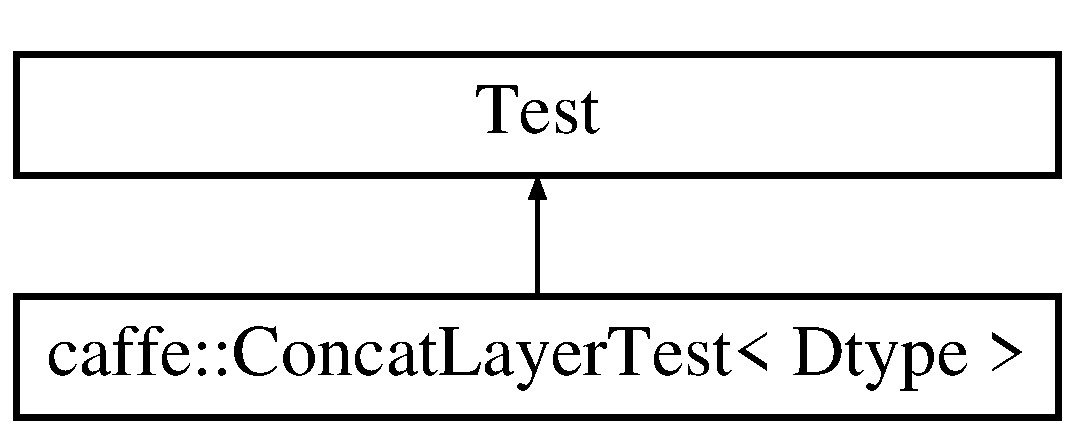
\includegraphics[height=2.000000cm]{classcaffe_1_1_concat_layer_test}
\end{center}
\end{figure}
\subsection*{Protected Member Functions}
\begin{DoxyCompactItemize}
\item 
\hyperlink{classcaffe_1_1_concat_layer_test_aee8ce0e8390e1c3753c5420202e5e598}{Concat\+Layer\+Test} ()
\item 
virtual void \hyperlink{classcaffe_1_1_concat_layer_test_a7c47be870fc60bab24bd882d64310401}{Set\+Up} ()
\item 
virtual \hyperlink{classcaffe_1_1_concat_layer_test_a66a184a925ea6949ffe9ae9140689227}{$\sim$\+Concat\+Layer\+Test} ()
\end{DoxyCompactItemize}
\subsection*{Protected Attributes}
\begin{DoxyCompactItemize}
\item 
\hyperlink{classcaffe_1_1_blob}{Blob}$<$ Dtype $>$ $\ast$const \hyperlink{classcaffe_1_1_concat_layer_test_a2aeb1f380b300d1adf464e5a9c7374bc}{blob\+\_\+bottom\+\_\+0}
\item 
\hyperlink{classcaffe_1_1_blob}{Blob}$<$ Dtype $>$ $\ast$const \hyperlink{classcaffe_1_1_concat_layer_test_a243aef5df87eadba613ca2b28c1b417b}{blob\+\_\+bottom\+\_\+1}
\item 
\hyperlink{classcaffe_1_1_blob}{Blob}$<$ Dtype $>$ $\ast$const \hyperlink{classcaffe_1_1_concat_layer_test_ac1adcb4ac23846de69e5225810b74c73}{blob\+\_\+bottom\+\_\+2}
\item 
\hyperlink{classcaffe_1_1_blob}{Blob}$<$ Dtype $>$ $\ast$const \hyperlink{classcaffe_1_1_concat_layer_test_ab04bb1208c677cf82e91534a897dec55}{blob\+\_\+top\+\_\+}
\item 
vector$<$ \hyperlink{classcaffe_1_1_blob}{Blob}$<$ Dtype $>$ $\ast$ $>$ \hyperlink{classcaffe_1_1_concat_layer_test_ad3d6992cf390bf791af61831658daaec}{blob\+\_\+bottom\+\_\+vec\+\_\+0}
\item 
vector$<$ \hyperlink{classcaffe_1_1_blob}{Blob}$<$ Dtype $>$ $\ast$ $>$ \hyperlink{classcaffe_1_1_concat_layer_test_aa5a6e553646415c58ff0457c66d60a0d}{blob\+\_\+bottom\+\_\+vec\+\_\+1}
\item 
vector$<$ \hyperlink{classcaffe_1_1_blob}{Blob}$<$ Dtype $>$ $\ast$ $>$ \hyperlink{classcaffe_1_1_concat_layer_test_ae891c1b8f80cebc4db0c50b2a8e958db}{blob\+\_\+top\+\_\+vec\+\_\+}
\end{DoxyCompactItemize}


\subsection{Constructor \& Destructor Documentation}
\hypertarget{classcaffe_1_1_concat_layer_test_aee8ce0e8390e1c3753c5420202e5e598}{\index{caffe\+::\+Concat\+Layer\+Test@{caffe\+::\+Concat\+Layer\+Test}!Concat\+Layer\+Test@{Concat\+Layer\+Test}}
\index{Concat\+Layer\+Test@{Concat\+Layer\+Test}!caffe\+::\+Concat\+Layer\+Test@{caffe\+::\+Concat\+Layer\+Test}}
\subsubsection[{Concat\+Layer\+Test}]{\setlength{\rightskip}{0pt plus 5cm}template$<$typename Dtype $>$ {\bf caffe\+::\+Concat\+Layer\+Test}$<$ Dtype $>$\+::{\bf Concat\+Layer\+Test} (
\begin{DoxyParamCaption}
{}
\end{DoxyParamCaption}
)\hspace{0.3cm}{\ttfamily [inline]}, {\ttfamily [protected]}}}\label{classcaffe_1_1_concat_layer_test_aee8ce0e8390e1c3753c5420202e5e598}
\hypertarget{classcaffe_1_1_concat_layer_test_a66a184a925ea6949ffe9ae9140689227}{\index{caffe\+::\+Concat\+Layer\+Test@{caffe\+::\+Concat\+Layer\+Test}!````~Concat\+Layer\+Test@{$\sim$\+Concat\+Layer\+Test}}
\index{````~Concat\+Layer\+Test@{$\sim$\+Concat\+Layer\+Test}!caffe\+::\+Concat\+Layer\+Test@{caffe\+::\+Concat\+Layer\+Test}}
\subsubsection[{$\sim$\+Concat\+Layer\+Test}]{\setlength{\rightskip}{0pt plus 5cm}template$<$typename Dtype $>$ virtual {\bf caffe\+::\+Concat\+Layer\+Test}$<$ Dtype $>$\+::$\sim${\bf Concat\+Layer\+Test} (
\begin{DoxyParamCaption}
{}
\end{DoxyParamCaption}
)\hspace{0.3cm}{\ttfamily [inline]}, {\ttfamily [protected]}, {\ttfamily [virtual]}}}\label{classcaffe_1_1_concat_layer_test_a66a184a925ea6949ffe9ae9140689227}


\subsection{Member Function Documentation}
\hypertarget{classcaffe_1_1_concat_layer_test_a7c47be870fc60bab24bd882d64310401}{\index{caffe\+::\+Concat\+Layer\+Test@{caffe\+::\+Concat\+Layer\+Test}!Set\+Up@{Set\+Up}}
\index{Set\+Up@{Set\+Up}!caffe\+::\+Concat\+Layer\+Test@{caffe\+::\+Concat\+Layer\+Test}}
\subsubsection[{Set\+Up}]{\setlength{\rightskip}{0pt plus 5cm}template$<$typename Dtype $>$ virtual void {\bf caffe\+::\+Concat\+Layer\+Test}$<$ Dtype $>$\+::Set\+Up (
\begin{DoxyParamCaption}
{}
\end{DoxyParamCaption}
)\hspace{0.3cm}{\ttfamily [inline]}, {\ttfamily [protected]}, {\ttfamily [virtual]}}}\label{classcaffe_1_1_concat_layer_test_a7c47be870fc60bab24bd882d64310401}


\subsection{Member Data Documentation}
\hypertarget{classcaffe_1_1_concat_layer_test_a2aeb1f380b300d1adf464e5a9c7374bc}{\index{caffe\+::\+Concat\+Layer\+Test@{caffe\+::\+Concat\+Layer\+Test}!blob\+\_\+bottom\+\_\+0@{blob\+\_\+bottom\+\_\+0}}
\index{blob\+\_\+bottom\+\_\+0@{blob\+\_\+bottom\+\_\+0}!caffe\+::\+Concat\+Layer\+Test@{caffe\+::\+Concat\+Layer\+Test}}
\subsubsection[{blob\+\_\+bottom\+\_\+0}]{\setlength{\rightskip}{0pt plus 5cm}template$<$typename Dtype $>$ {\bf Blob}$<$Dtype$>$$\ast$ const {\bf caffe\+::\+Concat\+Layer\+Test}$<$ Dtype $>$\+::blob\+\_\+bottom\+\_\+0\hspace{0.3cm}{\ttfamily [protected]}}}\label{classcaffe_1_1_concat_layer_test_a2aeb1f380b300d1adf464e5a9c7374bc}
\hypertarget{classcaffe_1_1_concat_layer_test_a243aef5df87eadba613ca2b28c1b417b}{\index{caffe\+::\+Concat\+Layer\+Test@{caffe\+::\+Concat\+Layer\+Test}!blob\+\_\+bottom\+\_\+1@{blob\+\_\+bottom\+\_\+1}}
\index{blob\+\_\+bottom\+\_\+1@{blob\+\_\+bottom\+\_\+1}!caffe\+::\+Concat\+Layer\+Test@{caffe\+::\+Concat\+Layer\+Test}}
\subsubsection[{blob\+\_\+bottom\+\_\+1}]{\setlength{\rightskip}{0pt plus 5cm}template$<$typename Dtype $>$ {\bf Blob}$<$Dtype$>$$\ast$ const {\bf caffe\+::\+Concat\+Layer\+Test}$<$ Dtype $>$\+::blob\+\_\+bottom\+\_\+1\hspace{0.3cm}{\ttfamily [protected]}}}\label{classcaffe_1_1_concat_layer_test_a243aef5df87eadba613ca2b28c1b417b}
\hypertarget{classcaffe_1_1_concat_layer_test_ac1adcb4ac23846de69e5225810b74c73}{\index{caffe\+::\+Concat\+Layer\+Test@{caffe\+::\+Concat\+Layer\+Test}!blob\+\_\+bottom\+\_\+2@{blob\+\_\+bottom\+\_\+2}}
\index{blob\+\_\+bottom\+\_\+2@{blob\+\_\+bottom\+\_\+2}!caffe\+::\+Concat\+Layer\+Test@{caffe\+::\+Concat\+Layer\+Test}}
\subsubsection[{blob\+\_\+bottom\+\_\+2}]{\setlength{\rightskip}{0pt plus 5cm}template$<$typename Dtype $>$ {\bf Blob}$<$Dtype$>$$\ast$ const {\bf caffe\+::\+Concat\+Layer\+Test}$<$ Dtype $>$\+::blob\+\_\+bottom\+\_\+2\hspace{0.3cm}{\ttfamily [protected]}}}\label{classcaffe_1_1_concat_layer_test_ac1adcb4ac23846de69e5225810b74c73}
\hypertarget{classcaffe_1_1_concat_layer_test_ad3d6992cf390bf791af61831658daaec}{\index{caffe\+::\+Concat\+Layer\+Test@{caffe\+::\+Concat\+Layer\+Test}!blob\+\_\+bottom\+\_\+vec\+\_\+0@{blob\+\_\+bottom\+\_\+vec\+\_\+0}}
\index{blob\+\_\+bottom\+\_\+vec\+\_\+0@{blob\+\_\+bottom\+\_\+vec\+\_\+0}!caffe\+::\+Concat\+Layer\+Test@{caffe\+::\+Concat\+Layer\+Test}}
\subsubsection[{blob\+\_\+bottom\+\_\+vec\+\_\+0}]{\setlength{\rightskip}{0pt plus 5cm}template$<$typename Dtype $>$ vector$<${\bf Blob}$<$Dtype$>$$\ast$$>$ {\bf caffe\+::\+Concat\+Layer\+Test}$<$ Dtype $>$\+::blob\+\_\+bottom\+\_\+vec\+\_\+0\hspace{0.3cm}{\ttfamily [protected]}}}\label{classcaffe_1_1_concat_layer_test_ad3d6992cf390bf791af61831658daaec}
\hypertarget{classcaffe_1_1_concat_layer_test_aa5a6e553646415c58ff0457c66d60a0d}{\index{caffe\+::\+Concat\+Layer\+Test@{caffe\+::\+Concat\+Layer\+Test}!blob\+\_\+bottom\+\_\+vec\+\_\+1@{blob\+\_\+bottom\+\_\+vec\+\_\+1}}
\index{blob\+\_\+bottom\+\_\+vec\+\_\+1@{blob\+\_\+bottom\+\_\+vec\+\_\+1}!caffe\+::\+Concat\+Layer\+Test@{caffe\+::\+Concat\+Layer\+Test}}
\subsubsection[{blob\+\_\+bottom\+\_\+vec\+\_\+1}]{\setlength{\rightskip}{0pt plus 5cm}template$<$typename Dtype $>$ vector$<${\bf Blob}$<$Dtype$>$$\ast$$>$ {\bf caffe\+::\+Concat\+Layer\+Test}$<$ Dtype $>$\+::blob\+\_\+bottom\+\_\+vec\+\_\+1\hspace{0.3cm}{\ttfamily [protected]}}}\label{classcaffe_1_1_concat_layer_test_aa5a6e553646415c58ff0457c66d60a0d}
\hypertarget{classcaffe_1_1_concat_layer_test_ab04bb1208c677cf82e91534a897dec55}{\index{caffe\+::\+Concat\+Layer\+Test@{caffe\+::\+Concat\+Layer\+Test}!blob\+\_\+top\+\_\+@{blob\+\_\+top\+\_\+}}
\index{blob\+\_\+top\+\_\+@{blob\+\_\+top\+\_\+}!caffe\+::\+Concat\+Layer\+Test@{caffe\+::\+Concat\+Layer\+Test}}
\subsubsection[{blob\+\_\+top\+\_\+}]{\setlength{\rightskip}{0pt plus 5cm}template$<$typename Dtype $>$ {\bf Blob}$<$Dtype$>$$\ast$ const {\bf caffe\+::\+Concat\+Layer\+Test}$<$ Dtype $>$\+::blob\+\_\+top\+\_\+\hspace{0.3cm}{\ttfamily [protected]}}}\label{classcaffe_1_1_concat_layer_test_ab04bb1208c677cf82e91534a897dec55}
\hypertarget{classcaffe_1_1_concat_layer_test_ae891c1b8f80cebc4db0c50b2a8e958db}{\index{caffe\+::\+Concat\+Layer\+Test@{caffe\+::\+Concat\+Layer\+Test}!blob\+\_\+top\+\_\+vec\+\_\+@{blob\+\_\+top\+\_\+vec\+\_\+}}
\index{blob\+\_\+top\+\_\+vec\+\_\+@{blob\+\_\+top\+\_\+vec\+\_\+}!caffe\+::\+Concat\+Layer\+Test@{caffe\+::\+Concat\+Layer\+Test}}
\subsubsection[{blob\+\_\+top\+\_\+vec\+\_\+}]{\setlength{\rightskip}{0pt plus 5cm}template$<$typename Dtype $>$ vector$<${\bf Blob}$<$Dtype$>$$\ast$$>$ {\bf caffe\+::\+Concat\+Layer\+Test}$<$ Dtype $>$\+::blob\+\_\+top\+\_\+vec\+\_\+\hspace{0.3cm}{\ttfamily [protected]}}}\label{classcaffe_1_1_concat_layer_test_ae891c1b8f80cebc4db0c50b2a8e958db}


The documentation for this class was generated from the following file\+:\begin{DoxyCompactItemize}
\item 
src/caffe/test/\hyperlink{test__concat__layer_8cpp}{test\+\_\+concat\+\_\+layer.\+cpp}\end{DoxyCompactItemize}

\hypertarget{classcaffe_1_1_constant_filler}{\section{caffe\+:\+:Constant\+Filler$<$ Dtype $>$ Class Template Reference}
\label{classcaffe_1_1_constant_filler}\index{caffe\+::\+Constant\+Filler$<$ Dtype $>$@{caffe\+::\+Constant\+Filler$<$ Dtype $>$}}
}


{\ttfamily \#include $<$filler.\+hpp$>$}

Inheritance diagram for caffe\+:\+:Constant\+Filler$<$ Dtype $>$\+:\begin{figure}[H]
\begin{center}
\leavevmode
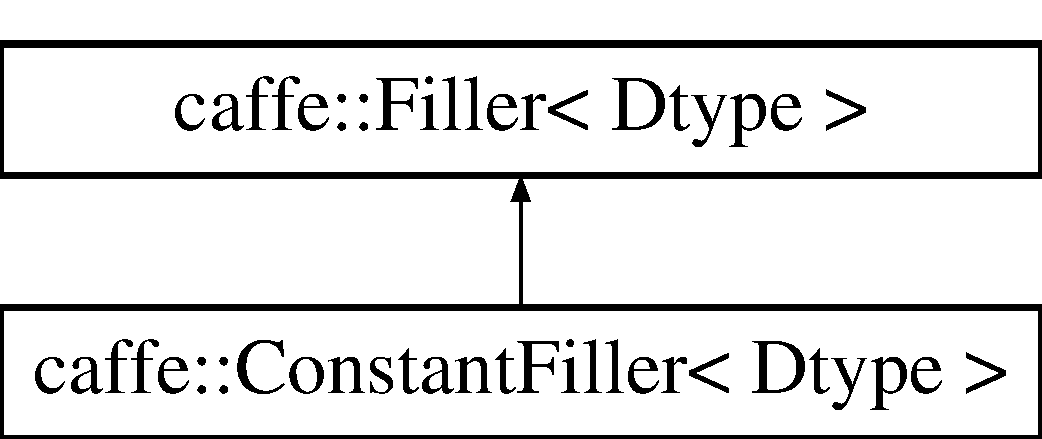
\includegraphics[height=2.000000cm]{classcaffe_1_1_constant_filler}
\end{center}
\end{figure}
\subsection*{Public Member Functions}
\begin{DoxyCompactItemize}
\item 
\hyperlink{classcaffe_1_1_constant_filler_ac6bd25bc764935cb5261d0279a772001}{Constant\+Filler} (const Filler\+Parameter \&param)
\item 
virtual void \hyperlink{classcaffe_1_1_constant_filler_a411cf44b177109c388c0b34c906f4e8e}{Fill} (\hyperlink{classcaffe_1_1_blob}{Blob}$<$ Dtype $>$ $\ast$blob)
\end{DoxyCompactItemize}
\subsection*{Additional Inherited Members}


\subsection{Constructor \& Destructor Documentation}
\hypertarget{classcaffe_1_1_constant_filler_ac6bd25bc764935cb5261d0279a772001}{\index{caffe\+::\+Constant\+Filler@{caffe\+::\+Constant\+Filler}!Constant\+Filler@{Constant\+Filler}}
\index{Constant\+Filler@{Constant\+Filler}!caffe\+::\+Constant\+Filler@{caffe\+::\+Constant\+Filler}}
\subsubsection[{Constant\+Filler}]{\setlength{\rightskip}{0pt plus 5cm}template$<$typename Dtype $>$ {\bf caffe\+::\+Constant\+Filler}$<$ Dtype $>$\+::{\bf Constant\+Filler} (
\begin{DoxyParamCaption}
\item[{const Filler\+Parameter \&}]{param}
\end{DoxyParamCaption}
)\hspace{0.3cm}{\ttfamily [inline]}, {\ttfamily [explicit]}}}\label{classcaffe_1_1_constant_filler_ac6bd25bc764935cb5261d0279a772001}


\subsection{Member Function Documentation}
\hypertarget{classcaffe_1_1_constant_filler_a411cf44b177109c388c0b34c906f4e8e}{\index{caffe\+::\+Constant\+Filler@{caffe\+::\+Constant\+Filler}!Fill@{Fill}}
\index{Fill@{Fill}!caffe\+::\+Constant\+Filler@{caffe\+::\+Constant\+Filler}}
\subsubsection[{Fill}]{\setlength{\rightskip}{0pt plus 5cm}template$<$typename Dtype $>$ virtual void {\bf caffe\+::\+Constant\+Filler}$<$ Dtype $>$\+::Fill (
\begin{DoxyParamCaption}
\item[{{\bf Blob}$<$ Dtype $>$ $\ast$}]{blob}
\end{DoxyParamCaption}
)\hspace{0.3cm}{\ttfamily [inline]}, {\ttfamily [virtual]}}}\label{classcaffe_1_1_constant_filler_a411cf44b177109c388c0b34c906f4e8e}


Implements \hyperlink{classcaffe_1_1_filler_acd02177b669381252a7c484f51432d30}{caffe\+::\+Filler$<$ Dtype $>$}.



The documentation for this class was generated from the following file\+:\begin{DoxyCompactItemize}
\item 
include/caffe/\hyperlink{filler_8hpp}{filler.\+hpp}\end{DoxyCompactItemize}

\hypertarget{classcaffe_1_1_constant_filler_test}{\section{caffe\+:\+:Constant\+Filler\+Test$<$ Dtype $>$ Class Template Reference}
\label{classcaffe_1_1_constant_filler_test}\index{caffe\+::\+Constant\+Filler\+Test$<$ Dtype $>$@{caffe\+::\+Constant\+Filler\+Test$<$ Dtype $>$}}
}
Inheritance diagram for caffe\+:\+:Constant\+Filler\+Test$<$ Dtype $>$\+:\begin{figure}[H]
\begin{center}
\leavevmode
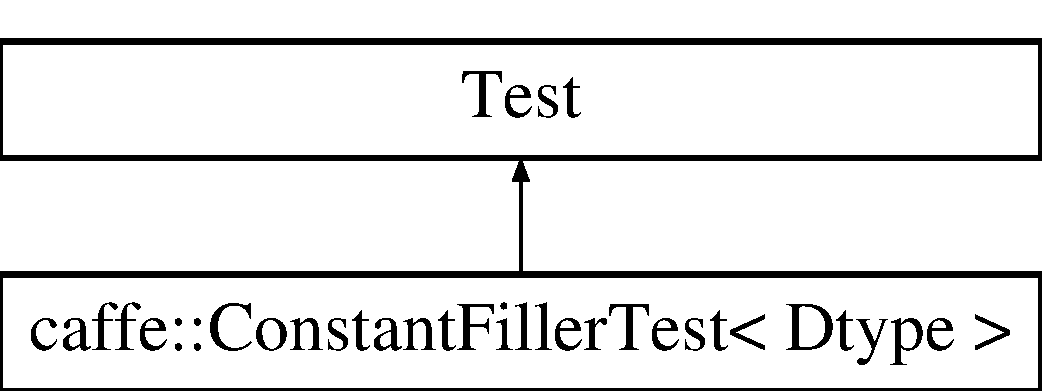
\includegraphics[height=2.000000cm]{classcaffe_1_1_constant_filler_test}
\end{center}
\end{figure}
\subsection*{Protected Member Functions}
\begin{DoxyCompactItemize}
\item 
\hyperlink{classcaffe_1_1_constant_filler_test_a7d87f98846e7e8a811f93c75afb1eb6e}{Constant\+Filler\+Test} ()
\item 
virtual \hyperlink{classcaffe_1_1_constant_filler_test_ace957505dc9394783212875ed4d89d3c}{$\sim$\+Constant\+Filler\+Test} ()
\end{DoxyCompactItemize}
\subsection*{Protected Attributes}
\begin{DoxyCompactItemize}
\item 
\hyperlink{classcaffe_1_1_blob}{Blob}$<$ Dtype $>$ $\ast$const \hyperlink{classcaffe_1_1_constant_filler_test_a3c61da8de712122294a6b0df36f9f6a7}{blob\+\_\+}
\item 
Filler\+Parameter \hyperlink{classcaffe_1_1_constant_filler_test_ae7c14a37c8b6370fc539cd82fb90d972}{filler\+\_\+param\+\_\+}
\item 
shared\+\_\+ptr$<$ \hyperlink{classcaffe_1_1_constant_filler}{Constant\+Filler}\\*
$<$ Dtype $>$ $>$ \hyperlink{classcaffe_1_1_constant_filler_test_adc3aca9d62166a3d14202317bbb89a3d}{filler\+\_\+}
\end{DoxyCompactItemize}


\subsection{Constructor \& Destructor Documentation}
\hypertarget{classcaffe_1_1_constant_filler_test_a7d87f98846e7e8a811f93c75afb1eb6e}{\index{caffe\+::\+Constant\+Filler\+Test@{caffe\+::\+Constant\+Filler\+Test}!Constant\+Filler\+Test@{Constant\+Filler\+Test}}
\index{Constant\+Filler\+Test@{Constant\+Filler\+Test}!caffe\+::\+Constant\+Filler\+Test@{caffe\+::\+Constant\+Filler\+Test}}
\subsubsection[{Constant\+Filler\+Test}]{\setlength{\rightskip}{0pt plus 5cm}template$<$typename Dtype $>$ {\bf caffe\+::\+Constant\+Filler\+Test}$<$ Dtype $>$\+::{\bf Constant\+Filler\+Test} (
\begin{DoxyParamCaption}
{}
\end{DoxyParamCaption}
)\hspace{0.3cm}{\ttfamily [inline]}, {\ttfamily [protected]}}}\label{classcaffe_1_1_constant_filler_test_a7d87f98846e7e8a811f93c75afb1eb6e}
\hypertarget{classcaffe_1_1_constant_filler_test_ace957505dc9394783212875ed4d89d3c}{\index{caffe\+::\+Constant\+Filler\+Test@{caffe\+::\+Constant\+Filler\+Test}!````~Constant\+Filler\+Test@{$\sim$\+Constant\+Filler\+Test}}
\index{````~Constant\+Filler\+Test@{$\sim$\+Constant\+Filler\+Test}!caffe\+::\+Constant\+Filler\+Test@{caffe\+::\+Constant\+Filler\+Test}}
\subsubsection[{$\sim$\+Constant\+Filler\+Test}]{\setlength{\rightskip}{0pt plus 5cm}template$<$typename Dtype $>$ virtual {\bf caffe\+::\+Constant\+Filler\+Test}$<$ Dtype $>$\+::$\sim${\bf Constant\+Filler\+Test} (
\begin{DoxyParamCaption}
{}
\end{DoxyParamCaption}
)\hspace{0.3cm}{\ttfamily [inline]}, {\ttfamily [protected]}, {\ttfamily [virtual]}}}\label{classcaffe_1_1_constant_filler_test_ace957505dc9394783212875ed4d89d3c}


\subsection{Member Data Documentation}
\hypertarget{classcaffe_1_1_constant_filler_test_a3c61da8de712122294a6b0df36f9f6a7}{\index{caffe\+::\+Constant\+Filler\+Test@{caffe\+::\+Constant\+Filler\+Test}!blob\+\_\+@{blob\+\_\+}}
\index{blob\+\_\+@{blob\+\_\+}!caffe\+::\+Constant\+Filler\+Test@{caffe\+::\+Constant\+Filler\+Test}}
\subsubsection[{blob\+\_\+}]{\setlength{\rightskip}{0pt plus 5cm}template$<$typename Dtype $>$ {\bf Blob}$<$Dtype$>$$\ast$ const {\bf caffe\+::\+Constant\+Filler\+Test}$<$ Dtype $>$\+::blob\+\_\+\hspace{0.3cm}{\ttfamily [protected]}}}\label{classcaffe_1_1_constant_filler_test_a3c61da8de712122294a6b0df36f9f6a7}
\hypertarget{classcaffe_1_1_constant_filler_test_adc3aca9d62166a3d14202317bbb89a3d}{\index{caffe\+::\+Constant\+Filler\+Test@{caffe\+::\+Constant\+Filler\+Test}!filler\+\_\+@{filler\+\_\+}}
\index{filler\+\_\+@{filler\+\_\+}!caffe\+::\+Constant\+Filler\+Test@{caffe\+::\+Constant\+Filler\+Test}}
\subsubsection[{filler\+\_\+}]{\setlength{\rightskip}{0pt plus 5cm}template$<$typename Dtype $>$ shared\+\_\+ptr$<${\bf Constant\+Filler}$<$Dtype$>$ $>$ {\bf caffe\+::\+Constant\+Filler\+Test}$<$ Dtype $>$\+::filler\+\_\+\hspace{0.3cm}{\ttfamily [protected]}}}\label{classcaffe_1_1_constant_filler_test_adc3aca9d62166a3d14202317bbb89a3d}
\hypertarget{classcaffe_1_1_constant_filler_test_ae7c14a37c8b6370fc539cd82fb90d972}{\index{caffe\+::\+Constant\+Filler\+Test@{caffe\+::\+Constant\+Filler\+Test}!filler\+\_\+param\+\_\+@{filler\+\_\+param\+\_\+}}
\index{filler\+\_\+param\+\_\+@{filler\+\_\+param\+\_\+}!caffe\+::\+Constant\+Filler\+Test@{caffe\+::\+Constant\+Filler\+Test}}
\subsubsection[{filler\+\_\+param\+\_\+}]{\setlength{\rightskip}{0pt plus 5cm}template$<$typename Dtype $>$ Filler\+Parameter {\bf caffe\+::\+Constant\+Filler\+Test}$<$ Dtype $>$\+::filler\+\_\+param\+\_\+\hspace{0.3cm}{\ttfamily [protected]}}}\label{classcaffe_1_1_constant_filler_test_ae7c14a37c8b6370fc539cd82fb90d972}


The documentation for this class was generated from the following file\+:\begin{DoxyCompactItemize}
\item 
src/caffe/test/\hyperlink{test__filler_8cpp}{test\+\_\+filler.\+cpp}\end{DoxyCompactItemize}

\hypertarget{classcaffe_1_1_convolution_layer}{\section{caffe\+:\+:Convolution\+Layer$<$ Dtype $>$ Class Template Reference}
\label{classcaffe_1_1_convolution_layer}\index{caffe\+::\+Convolution\+Layer$<$ Dtype $>$@{caffe\+::\+Convolution\+Layer$<$ Dtype $>$}}
}


{\ttfamily \#include $<$vision\+\_\+layers.\+hpp$>$}

Inheritance diagram for caffe\+:\+:Convolution\+Layer$<$ Dtype $>$\+:\begin{figure}[H]
\begin{center}
\leavevmode
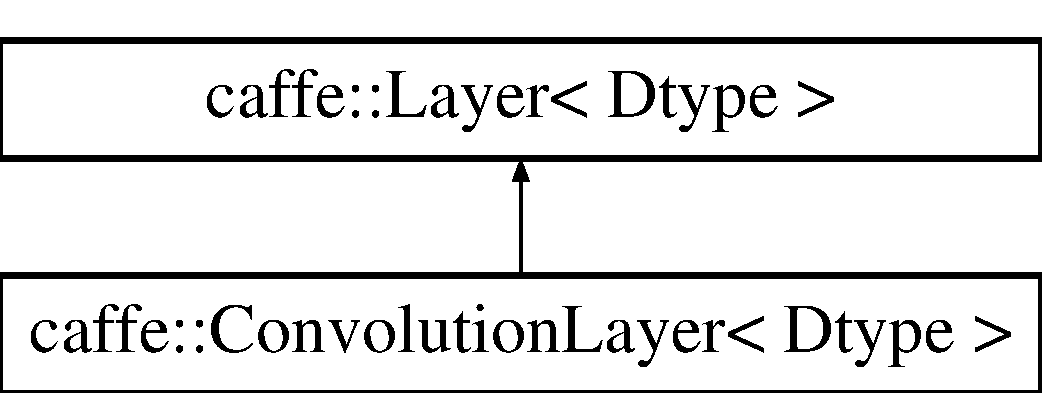
\includegraphics[height=2.000000cm]{classcaffe_1_1_convolution_layer}
\end{center}
\end{figure}
\subsection*{Public Member Functions}
\begin{DoxyCompactItemize}
\item 
\hyperlink{classcaffe_1_1_convolution_layer_ad27360afd7729001b9e4f1d8c8401866}{Convolution\+Layer} (const Layer\+Parameter \&param)
\item 
virtual void \hyperlink{classcaffe_1_1_convolution_layer_ad3eebbeb87db98a784aea2ddd8e8199d}{Set\+Up} (const vector$<$ \hyperlink{classcaffe_1_1_blob}{Blob}$<$ Dtype $>$ $\ast$ $>$ \&bottom, vector$<$ \hyperlink{classcaffe_1_1_blob}{Blob}$<$ Dtype $>$ $\ast$ $>$ $\ast$top)
\end{DoxyCompactItemize}
\subsection*{Protected Member Functions}
\begin{DoxyCompactItemize}
\item 
virtual Dtype \hyperlink{classcaffe_1_1_convolution_layer_a53eb4114d914f019bc873818d4f8e53b}{Forward\+\_\+cpu} (const vector$<$ \hyperlink{classcaffe_1_1_blob}{Blob}$<$ Dtype $>$ $\ast$ $>$ \&bottom, vector$<$ \hyperlink{classcaffe_1_1_blob}{Blob}$<$ Dtype $>$ $\ast$ $>$ $\ast$top)
\item 
virtual Dtype \hyperlink{classcaffe_1_1_convolution_layer_a1feac725539612918553e6b7bf299b4b}{Forward\+\_\+gpu} (const vector$<$ \hyperlink{classcaffe_1_1_blob}{Blob}$<$ Dtype $>$ $\ast$ $>$ \&bottom, vector$<$ \hyperlink{classcaffe_1_1_blob}{Blob}$<$ Dtype $>$ $\ast$ $>$ $\ast$top)
\item 
virtual void \hyperlink{classcaffe_1_1_convolution_layer_a977898d74cd37fa2557f74322d419575}{Backward\+\_\+cpu} (const vector$<$ \hyperlink{classcaffe_1_1_blob}{Blob}$<$ Dtype $>$ $\ast$ $>$ \&top, const bool propagate\+\_\+down, vector$<$ \hyperlink{classcaffe_1_1_blob}{Blob}$<$ Dtype $>$ $\ast$ $>$ $\ast$bottom)
\item 
virtual void \hyperlink{classcaffe_1_1_convolution_layer_a451a90070f9600b3bc33e0a9f9356ab2}{Backward\+\_\+gpu} (const vector$<$ \hyperlink{classcaffe_1_1_blob}{Blob}$<$ Dtype $>$ $\ast$ $>$ \&top, const bool propagate\+\_\+down, vector$<$ \hyperlink{classcaffe_1_1_blob}{Blob}$<$ Dtype $>$ $\ast$ $>$ $\ast$bottom)
\end{DoxyCompactItemize}
\subsection*{Protected Attributes}
\begin{DoxyCompactItemize}
\item 
int \hyperlink{classcaffe_1_1_convolution_layer_aa1ca915eb8f781f4b168aaf21f39894b}{kernel\+\_\+size\+\_\+}
\item 
int \hyperlink{classcaffe_1_1_convolution_layer_a3ba44963cfa4f1bbcdf141d0199bc493}{stride\+\_\+}
\item 
int \hyperlink{classcaffe_1_1_convolution_layer_a6976c8be8d083e9ebe44756b5bc6479b}{num\+\_\+}
\item 
int \hyperlink{classcaffe_1_1_convolution_layer_ad70d4cbdcb75695b05b13bc479445aec}{channels\+\_\+}
\item 
int \hyperlink{classcaffe_1_1_convolution_layer_aba61b8e2065eda304e35fa3fa753eb80}{pad\+\_\+}
\item 
int \hyperlink{classcaffe_1_1_convolution_layer_a647a6b1172a630ac5f8b8eee9ef4e7b2}{height\+\_\+}
\item 
int \hyperlink{classcaffe_1_1_convolution_layer_a8286a1369f876ad29cea7f3dcca4a3a7}{width\+\_\+}
\item 
int \hyperlink{classcaffe_1_1_convolution_layer_af58ade65cda5954b9467f82df8999b89}{num\+\_\+output\+\_\+}
\item 
int \hyperlink{classcaffe_1_1_convolution_layer_a0a6f9c53ba515998258a98d523ff72b0}{group\+\_\+}
\item 
\hyperlink{classcaffe_1_1_blob}{Blob}$<$ Dtype $>$ \hyperlink{classcaffe_1_1_convolution_layer_a26feaeca8bbd36a64e782ab2e12b46d2}{col\+\_\+buffer\+\_\+}
\item 
shared\+\_\+ptr$<$ \hyperlink{classcaffe_1_1_synced_memory}{Synced\+Memory} $>$ \hyperlink{classcaffe_1_1_convolution_layer_a587cf49430daaacbd570e6a97c4364d2}{bias\+\_\+multiplier\+\_\+}
\item 
bool \hyperlink{classcaffe_1_1_convolution_layer_a0e8fbac1d24ba656fa6593191b21b32b}{bias\+\_\+term\+\_\+}
\item 
int \hyperlink{classcaffe_1_1_convolution_layer_a6a5386d7cc7b6b53653cdc9d17925116}{M\+\_\+}
\item 
int \hyperlink{classcaffe_1_1_convolution_layer_a917cf494c7845d3be0234dad754d4f49}{K\+\_\+}
\item 
int \hyperlink{classcaffe_1_1_convolution_layer_ad10263fbb69959ac83dee14deadc5f61}{N\+\_\+}
\end{DoxyCompactItemize}


\subsection{Constructor \& Destructor Documentation}
\hypertarget{classcaffe_1_1_convolution_layer_ad27360afd7729001b9e4f1d8c8401866}{\index{caffe\+::\+Convolution\+Layer@{caffe\+::\+Convolution\+Layer}!Convolution\+Layer@{Convolution\+Layer}}
\index{Convolution\+Layer@{Convolution\+Layer}!caffe\+::\+Convolution\+Layer@{caffe\+::\+Convolution\+Layer}}
\subsubsection[{Convolution\+Layer}]{\setlength{\rightskip}{0pt plus 5cm}template$<$typename Dtype $>$ {\bf caffe\+::\+Convolution\+Layer}$<$ Dtype $>$\+::{\bf Convolution\+Layer} (
\begin{DoxyParamCaption}
\item[{const Layer\+Parameter \&}]{param}
\end{DoxyParamCaption}
)\hspace{0.3cm}{\ttfamily [inline]}, {\ttfamily [explicit]}}}\label{classcaffe_1_1_convolution_layer_ad27360afd7729001b9e4f1d8c8401866}


\subsection{Member Function Documentation}
\hypertarget{classcaffe_1_1_convolution_layer_a977898d74cd37fa2557f74322d419575}{\index{caffe\+::\+Convolution\+Layer@{caffe\+::\+Convolution\+Layer}!Backward\+\_\+cpu@{Backward\+\_\+cpu}}
\index{Backward\+\_\+cpu@{Backward\+\_\+cpu}!caffe\+::\+Convolution\+Layer@{caffe\+::\+Convolution\+Layer}}
\subsubsection[{Backward\+\_\+cpu}]{\setlength{\rightskip}{0pt plus 5cm}template$<$typename Dtype $>$ void {\bf caffe\+::\+Convolution\+Layer}$<$ Dtype $>$\+::Backward\+\_\+cpu (
\begin{DoxyParamCaption}
\item[{const vector$<$ {\bf Blob}$<$ Dtype $>$ $\ast$ $>$ \&}]{top, }
\item[{const bool}]{propagate\+\_\+down, }
\item[{vector$<$ {\bf Blob}$<$ Dtype $>$ $\ast$ $>$ $\ast$}]{bottom}
\end{DoxyParamCaption}
)\hspace{0.3cm}{\ttfamily [protected]}, {\ttfamily [virtual]}}}\label{classcaffe_1_1_convolution_layer_a977898d74cd37fa2557f74322d419575}


Implements \hyperlink{classcaffe_1_1_layer_ac2d82011d076237c67997f63e7ee4b80}{caffe\+::\+Layer$<$ Dtype $>$}.

\hypertarget{classcaffe_1_1_convolution_layer_a451a90070f9600b3bc33e0a9f9356ab2}{\index{caffe\+::\+Convolution\+Layer@{caffe\+::\+Convolution\+Layer}!Backward\+\_\+gpu@{Backward\+\_\+gpu}}
\index{Backward\+\_\+gpu@{Backward\+\_\+gpu}!caffe\+::\+Convolution\+Layer@{caffe\+::\+Convolution\+Layer}}
\subsubsection[{Backward\+\_\+gpu}]{\setlength{\rightskip}{0pt plus 5cm}template$<$typename Dtype $>$ void {\bf caffe\+::\+Convolution\+Layer}$<$ Dtype $>$\+::Backward\+\_\+gpu (
\begin{DoxyParamCaption}
\item[{const vector$<$ {\bf Blob}$<$ Dtype $>$ $\ast$ $>$ \&}]{top, }
\item[{const bool}]{propagate\+\_\+down, }
\item[{vector$<$ {\bf Blob}$<$ Dtype $>$ $\ast$ $>$ $\ast$}]{bottom}
\end{DoxyParamCaption}
)\hspace{0.3cm}{\ttfamily [protected]}, {\ttfamily [virtual]}}}\label{classcaffe_1_1_convolution_layer_a451a90070f9600b3bc33e0a9f9356ab2}


Reimplemented from \hyperlink{classcaffe_1_1_layer_adf07ffe1f22d2fd2b1b0ff475ef5a64b}{caffe\+::\+Layer$<$ Dtype $>$}.

\hypertarget{classcaffe_1_1_convolution_layer_a53eb4114d914f019bc873818d4f8e53b}{\index{caffe\+::\+Convolution\+Layer@{caffe\+::\+Convolution\+Layer}!Forward\+\_\+cpu@{Forward\+\_\+cpu}}
\index{Forward\+\_\+cpu@{Forward\+\_\+cpu}!caffe\+::\+Convolution\+Layer@{caffe\+::\+Convolution\+Layer}}
\subsubsection[{Forward\+\_\+cpu}]{\setlength{\rightskip}{0pt plus 5cm}template$<$typename Dtype $>$ Dtype {\bf caffe\+::\+Convolution\+Layer}$<$ Dtype $>$\+::Forward\+\_\+cpu (
\begin{DoxyParamCaption}
\item[{const vector$<$ {\bf Blob}$<$ Dtype $>$ $\ast$ $>$ \&}]{bottom, }
\item[{vector$<$ {\bf Blob}$<$ Dtype $>$ $\ast$ $>$ $\ast$}]{top}
\end{DoxyParamCaption}
)\hspace{0.3cm}{\ttfamily [protected]}, {\ttfamily [virtual]}}}\label{classcaffe_1_1_convolution_layer_a53eb4114d914f019bc873818d4f8e53b}


Implements \hyperlink{classcaffe_1_1_layer_a8f7f61da3b8b3ca7f2394dee33873353}{caffe\+::\+Layer$<$ Dtype $>$}.

\hypertarget{classcaffe_1_1_convolution_layer_a1feac725539612918553e6b7bf299b4b}{\index{caffe\+::\+Convolution\+Layer@{caffe\+::\+Convolution\+Layer}!Forward\+\_\+gpu@{Forward\+\_\+gpu}}
\index{Forward\+\_\+gpu@{Forward\+\_\+gpu}!caffe\+::\+Convolution\+Layer@{caffe\+::\+Convolution\+Layer}}
\subsubsection[{Forward\+\_\+gpu}]{\setlength{\rightskip}{0pt plus 5cm}template$<$typename Dtype $>$ Dtype {\bf caffe\+::\+Convolution\+Layer}$<$ Dtype $>$\+::Forward\+\_\+gpu (
\begin{DoxyParamCaption}
\item[{const vector$<$ {\bf Blob}$<$ Dtype $>$ $\ast$ $>$ \&}]{bottom, }
\item[{vector$<$ {\bf Blob}$<$ Dtype $>$ $\ast$ $>$ $\ast$}]{top}
\end{DoxyParamCaption}
)\hspace{0.3cm}{\ttfamily [protected]}, {\ttfamily [virtual]}}}\label{classcaffe_1_1_convolution_layer_a1feac725539612918553e6b7bf299b4b}


Reimplemented from \hyperlink{classcaffe_1_1_layer_a2d78dbf5d8bc36928bd8f6fcfbafbcef}{caffe\+::\+Layer$<$ Dtype $>$}.

\hypertarget{classcaffe_1_1_convolution_layer_ad3eebbeb87db98a784aea2ddd8e8199d}{\index{caffe\+::\+Convolution\+Layer@{caffe\+::\+Convolution\+Layer}!Set\+Up@{Set\+Up}}
\index{Set\+Up@{Set\+Up}!caffe\+::\+Convolution\+Layer@{caffe\+::\+Convolution\+Layer}}
\subsubsection[{Set\+Up}]{\setlength{\rightskip}{0pt plus 5cm}template$<$typename Dtype $>$ void {\bf caffe\+::\+Convolution\+Layer}$<$ Dtype $>$\+::Set\+Up (
\begin{DoxyParamCaption}
\item[{const vector$<$ {\bf Blob}$<$ Dtype $>$ $\ast$ $>$ \&}]{bottom, }
\item[{vector$<$ {\bf Blob}$<$ Dtype $>$ $\ast$ $>$ $\ast$}]{top}
\end{DoxyParamCaption}
)\hspace{0.3cm}{\ttfamily [virtual]}}}\label{classcaffe_1_1_convolution_layer_ad3eebbeb87db98a784aea2ddd8e8199d}


Implements \hyperlink{classcaffe_1_1_layer_abd13c6489c13953b4fbcfcf6880835d0}{caffe\+::\+Layer$<$ Dtype $>$}.



\subsection{Member Data Documentation}
\hypertarget{classcaffe_1_1_convolution_layer_a587cf49430daaacbd570e6a97c4364d2}{\index{caffe\+::\+Convolution\+Layer@{caffe\+::\+Convolution\+Layer}!bias\+\_\+multiplier\+\_\+@{bias\+\_\+multiplier\+\_\+}}
\index{bias\+\_\+multiplier\+\_\+@{bias\+\_\+multiplier\+\_\+}!caffe\+::\+Convolution\+Layer@{caffe\+::\+Convolution\+Layer}}
\subsubsection[{bias\+\_\+multiplier\+\_\+}]{\setlength{\rightskip}{0pt plus 5cm}template$<$typename Dtype $>$ shared\+\_\+ptr$<${\bf Synced\+Memory}$>$ {\bf caffe\+::\+Convolution\+Layer}$<$ Dtype $>$\+::bias\+\_\+multiplier\+\_\+\hspace{0.3cm}{\ttfamily [protected]}}}\label{classcaffe_1_1_convolution_layer_a587cf49430daaacbd570e6a97c4364d2}
\hypertarget{classcaffe_1_1_convolution_layer_a0e8fbac1d24ba656fa6593191b21b32b}{\index{caffe\+::\+Convolution\+Layer@{caffe\+::\+Convolution\+Layer}!bias\+\_\+term\+\_\+@{bias\+\_\+term\+\_\+}}
\index{bias\+\_\+term\+\_\+@{bias\+\_\+term\+\_\+}!caffe\+::\+Convolution\+Layer@{caffe\+::\+Convolution\+Layer}}
\subsubsection[{bias\+\_\+term\+\_\+}]{\setlength{\rightskip}{0pt plus 5cm}template$<$typename Dtype $>$ bool {\bf caffe\+::\+Convolution\+Layer}$<$ Dtype $>$\+::bias\+\_\+term\+\_\+\hspace{0.3cm}{\ttfamily [protected]}}}\label{classcaffe_1_1_convolution_layer_a0e8fbac1d24ba656fa6593191b21b32b}
\hypertarget{classcaffe_1_1_convolution_layer_ad70d4cbdcb75695b05b13bc479445aec}{\index{caffe\+::\+Convolution\+Layer@{caffe\+::\+Convolution\+Layer}!channels\+\_\+@{channels\+\_\+}}
\index{channels\+\_\+@{channels\+\_\+}!caffe\+::\+Convolution\+Layer@{caffe\+::\+Convolution\+Layer}}
\subsubsection[{channels\+\_\+}]{\setlength{\rightskip}{0pt plus 5cm}template$<$typename Dtype $>$ int {\bf caffe\+::\+Convolution\+Layer}$<$ Dtype $>$\+::channels\+\_\+\hspace{0.3cm}{\ttfamily [protected]}}}\label{classcaffe_1_1_convolution_layer_ad70d4cbdcb75695b05b13bc479445aec}
\hypertarget{classcaffe_1_1_convolution_layer_a26feaeca8bbd36a64e782ab2e12b46d2}{\index{caffe\+::\+Convolution\+Layer@{caffe\+::\+Convolution\+Layer}!col\+\_\+buffer\+\_\+@{col\+\_\+buffer\+\_\+}}
\index{col\+\_\+buffer\+\_\+@{col\+\_\+buffer\+\_\+}!caffe\+::\+Convolution\+Layer@{caffe\+::\+Convolution\+Layer}}
\subsubsection[{col\+\_\+buffer\+\_\+}]{\setlength{\rightskip}{0pt plus 5cm}template$<$typename Dtype $>$ {\bf Blob}$<$Dtype$>$ {\bf caffe\+::\+Convolution\+Layer}$<$ Dtype $>$\+::col\+\_\+buffer\+\_\+\hspace{0.3cm}{\ttfamily [protected]}}}\label{classcaffe_1_1_convolution_layer_a26feaeca8bbd36a64e782ab2e12b46d2}
\hypertarget{classcaffe_1_1_convolution_layer_a0a6f9c53ba515998258a98d523ff72b0}{\index{caffe\+::\+Convolution\+Layer@{caffe\+::\+Convolution\+Layer}!group\+\_\+@{group\+\_\+}}
\index{group\+\_\+@{group\+\_\+}!caffe\+::\+Convolution\+Layer@{caffe\+::\+Convolution\+Layer}}
\subsubsection[{group\+\_\+}]{\setlength{\rightskip}{0pt plus 5cm}template$<$typename Dtype $>$ int {\bf caffe\+::\+Convolution\+Layer}$<$ Dtype $>$\+::group\+\_\+\hspace{0.3cm}{\ttfamily [protected]}}}\label{classcaffe_1_1_convolution_layer_a0a6f9c53ba515998258a98d523ff72b0}
\hypertarget{classcaffe_1_1_convolution_layer_a647a6b1172a630ac5f8b8eee9ef4e7b2}{\index{caffe\+::\+Convolution\+Layer@{caffe\+::\+Convolution\+Layer}!height\+\_\+@{height\+\_\+}}
\index{height\+\_\+@{height\+\_\+}!caffe\+::\+Convolution\+Layer@{caffe\+::\+Convolution\+Layer}}
\subsubsection[{height\+\_\+}]{\setlength{\rightskip}{0pt plus 5cm}template$<$typename Dtype $>$ int {\bf caffe\+::\+Convolution\+Layer}$<$ Dtype $>$\+::height\+\_\+\hspace{0.3cm}{\ttfamily [protected]}}}\label{classcaffe_1_1_convolution_layer_a647a6b1172a630ac5f8b8eee9ef4e7b2}
\hypertarget{classcaffe_1_1_convolution_layer_a917cf494c7845d3be0234dad754d4f49}{\index{caffe\+::\+Convolution\+Layer@{caffe\+::\+Convolution\+Layer}!K\+\_\+@{K\+\_\+}}
\index{K\+\_\+@{K\+\_\+}!caffe\+::\+Convolution\+Layer@{caffe\+::\+Convolution\+Layer}}
\subsubsection[{K\+\_\+}]{\setlength{\rightskip}{0pt plus 5cm}template$<$typename Dtype $>$ int {\bf caffe\+::\+Convolution\+Layer}$<$ Dtype $>$\+::K\+\_\+\hspace{0.3cm}{\ttfamily [protected]}}}\label{classcaffe_1_1_convolution_layer_a917cf494c7845d3be0234dad754d4f49}
\hypertarget{classcaffe_1_1_convolution_layer_aa1ca915eb8f781f4b168aaf21f39894b}{\index{caffe\+::\+Convolution\+Layer@{caffe\+::\+Convolution\+Layer}!kernel\+\_\+size\+\_\+@{kernel\+\_\+size\+\_\+}}
\index{kernel\+\_\+size\+\_\+@{kernel\+\_\+size\+\_\+}!caffe\+::\+Convolution\+Layer@{caffe\+::\+Convolution\+Layer}}
\subsubsection[{kernel\+\_\+size\+\_\+}]{\setlength{\rightskip}{0pt plus 5cm}template$<$typename Dtype $>$ int {\bf caffe\+::\+Convolution\+Layer}$<$ Dtype $>$\+::kernel\+\_\+size\+\_\+\hspace{0.3cm}{\ttfamily [protected]}}}\label{classcaffe_1_1_convolution_layer_aa1ca915eb8f781f4b168aaf21f39894b}
\hypertarget{classcaffe_1_1_convolution_layer_a6a5386d7cc7b6b53653cdc9d17925116}{\index{caffe\+::\+Convolution\+Layer@{caffe\+::\+Convolution\+Layer}!M\+\_\+@{M\+\_\+}}
\index{M\+\_\+@{M\+\_\+}!caffe\+::\+Convolution\+Layer@{caffe\+::\+Convolution\+Layer}}
\subsubsection[{M\+\_\+}]{\setlength{\rightskip}{0pt plus 5cm}template$<$typename Dtype $>$ int {\bf caffe\+::\+Convolution\+Layer}$<$ Dtype $>$\+::M\+\_\+\hspace{0.3cm}{\ttfamily [protected]}}}\label{classcaffe_1_1_convolution_layer_a6a5386d7cc7b6b53653cdc9d17925116}
\hypertarget{classcaffe_1_1_convolution_layer_ad10263fbb69959ac83dee14deadc5f61}{\index{caffe\+::\+Convolution\+Layer@{caffe\+::\+Convolution\+Layer}!N\+\_\+@{N\+\_\+}}
\index{N\+\_\+@{N\+\_\+}!caffe\+::\+Convolution\+Layer@{caffe\+::\+Convolution\+Layer}}
\subsubsection[{N\+\_\+}]{\setlength{\rightskip}{0pt plus 5cm}template$<$typename Dtype $>$ int {\bf caffe\+::\+Convolution\+Layer}$<$ Dtype $>$\+::N\+\_\+\hspace{0.3cm}{\ttfamily [protected]}}}\label{classcaffe_1_1_convolution_layer_ad10263fbb69959ac83dee14deadc5f61}
\hypertarget{classcaffe_1_1_convolution_layer_a6976c8be8d083e9ebe44756b5bc6479b}{\index{caffe\+::\+Convolution\+Layer@{caffe\+::\+Convolution\+Layer}!num\+\_\+@{num\+\_\+}}
\index{num\+\_\+@{num\+\_\+}!caffe\+::\+Convolution\+Layer@{caffe\+::\+Convolution\+Layer}}
\subsubsection[{num\+\_\+}]{\setlength{\rightskip}{0pt plus 5cm}template$<$typename Dtype $>$ int {\bf caffe\+::\+Convolution\+Layer}$<$ Dtype $>$\+::num\+\_\+\hspace{0.3cm}{\ttfamily [protected]}}}\label{classcaffe_1_1_convolution_layer_a6976c8be8d083e9ebe44756b5bc6479b}
\hypertarget{classcaffe_1_1_convolution_layer_af58ade65cda5954b9467f82df8999b89}{\index{caffe\+::\+Convolution\+Layer@{caffe\+::\+Convolution\+Layer}!num\+\_\+output\+\_\+@{num\+\_\+output\+\_\+}}
\index{num\+\_\+output\+\_\+@{num\+\_\+output\+\_\+}!caffe\+::\+Convolution\+Layer@{caffe\+::\+Convolution\+Layer}}
\subsubsection[{num\+\_\+output\+\_\+}]{\setlength{\rightskip}{0pt plus 5cm}template$<$typename Dtype $>$ int {\bf caffe\+::\+Convolution\+Layer}$<$ Dtype $>$\+::num\+\_\+output\+\_\+\hspace{0.3cm}{\ttfamily [protected]}}}\label{classcaffe_1_1_convolution_layer_af58ade65cda5954b9467f82df8999b89}
\hypertarget{classcaffe_1_1_convolution_layer_aba61b8e2065eda304e35fa3fa753eb80}{\index{caffe\+::\+Convolution\+Layer@{caffe\+::\+Convolution\+Layer}!pad\+\_\+@{pad\+\_\+}}
\index{pad\+\_\+@{pad\+\_\+}!caffe\+::\+Convolution\+Layer@{caffe\+::\+Convolution\+Layer}}
\subsubsection[{pad\+\_\+}]{\setlength{\rightskip}{0pt plus 5cm}template$<$typename Dtype $>$ int {\bf caffe\+::\+Convolution\+Layer}$<$ Dtype $>$\+::pad\+\_\+\hspace{0.3cm}{\ttfamily [protected]}}}\label{classcaffe_1_1_convolution_layer_aba61b8e2065eda304e35fa3fa753eb80}
\hypertarget{classcaffe_1_1_convolution_layer_a3ba44963cfa4f1bbcdf141d0199bc493}{\index{caffe\+::\+Convolution\+Layer@{caffe\+::\+Convolution\+Layer}!stride\+\_\+@{stride\+\_\+}}
\index{stride\+\_\+@{stride\+\_\+}!caffe\+::\+Convolution\+Layer@{caffe\+::\+Convolution\+Layer}}
\subsubsection[{stride\+\_\+}]{\setlength{\rightskip}{0pt plus 5cm}template$<$typename Dtype $>$ int {\bf caffe\+::\+Convolution\+Layer}$<$ Dtype $>$\+::stride\+\_\+\hspace{0.3cm}{\ttfamily [protected]}}}\label{classcaffe_1_1_convolution_layer_a3ba44963cfa4f1bbcdf141d0199bc493}
\hypertarget{classcaffe_1_1_convolution_layer_a8286a1369f876ad29cea7f3dcca4a3a7}{\index{caffe\+::\+Convolution\+Layer@{caffe\+::\+Convolution\+Layer}!width\+\_\+@{width\+\_\+}}
\index{width\+\_\+@{width\+\_\+}!caffe\+::\+Convolution\+Layer@{caffe\+::\+Convolution\+Layer}}
\subsubsection[{width\+\_\+}]{\setlength{\rightskip}{0pt plus 5cm}template$<$typename Dtype $>$ int {\bf caffe\+::\+Convolution\+Layer}$<$ Dtype $>$\+::width\+\_\+\hspace{0.3cm}{\ttfamily [protected]}}}\label{classcaffe_1_1_convolution_layer_a8286a1369f876ad29cea7f3dcca4a3a7}


The documentation for this class was generated from the following files\+:\begin{DoxyCompactItemize}
\item 
include/caffe/\hyperlink{vision__layers_8hpp}{vision\+\_\+layers.\+hpp}\item 
src/caffe/layers/\hyperlink{conv__layer_8cpp}{conv\+\_\+layer.\+cpp}\item 
src/caffe/layers/\hyperlink{conv__layer_8cu}{conv\+\_\+layer.\+cu}\end{DoxyCompactItemize}

\hypertarget{classcaffe_1_1_convolution_layer_test}{\section{caffe\+:\+:Convolution\+Layer\+Test$<$ Dtype $>$ Class Template Reference}
\label{classcaffe_1_1_convolution_layer_test}\index{caffe\+::\+Convolution\+Layer\+Test$<$ Dtype $>$@{caffe\+::\+Convolution\+Layer\+Test$<$ Dtype $>$}}
}
Inheritance diagram for caffe\+:\+:Convolution\+Layer\+Test$<$ Dtype $>$\+:\begin{figure}[H]
\begin{center}
\leavevmode
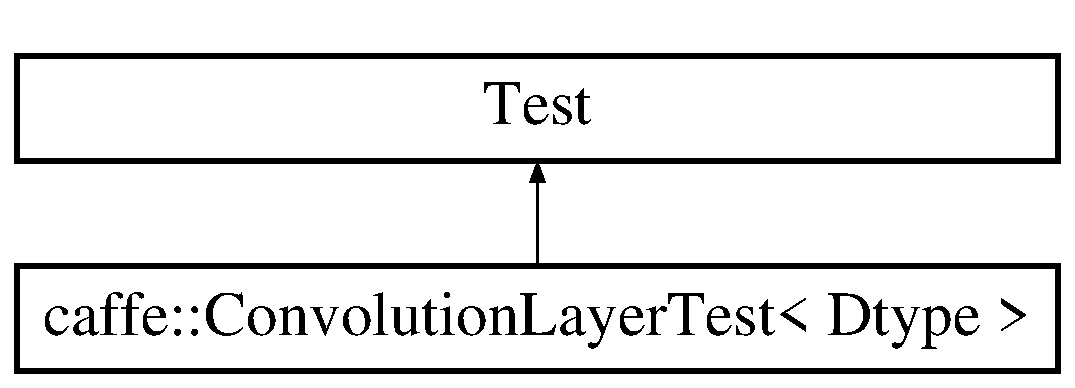
\includegraphics[height=2.000000cm]{classcaffe_1_1_convolution_layer_test}
\end{center}
\end{figure}
\subsection*{Protected Member Functions}
\begin{DoxyCompactItemize}
\item 
\hyperlink{classcaffe_1_1_convolution_layer_test_a9b7ea9083334a05ed4e8391b93fe8de2}{Convolution\+Layer\+Test} ()
\item 
virtual void \hyperlink{classcaffe_1_1_convolution_layer_test_aa7eb509c8c41313e372a3bfdd0e010d0}{Set\+Up} ()
\item 
virtual \hyperlink{classcaffe_1_1_convolution_layer_test_aa819ddf3e86c7f47c71c958722051d3b}{$\sim$\+Convolution\+Layer\+Test} ()
\end{DoxyCompactItemize}
\subsection*{Protected Attributes}
\begin{DoxyCompactItemize}
\item 
\hyperlink{classcaffe_1_1_blob}{Blob}$<$ Dtype $>$ $\ast$const \hyperlink{classcaffe_1_1_convolution_layer_test_a21716aea5f577453a99d8e3b81a3d5c1}{blob\+\_\+bottom\+\_\+}
\item 
\hyperlink{classcaffe_1_1_blob}{Blob}$<$ Dtype $>$ $\ast$const \hyperlink{classcaffe_1_1_convolution_layer_test_a46f8f672a46471f36229b33353b74819}{blob\+\_\+top\+\_\+}
\item 
vector$<$ \hyperlink{classcaffe_1_1_blob}{Blob}$<$ Dtype $>$ $\ast$ $>$ \hyperlink{classcaffe_1_1_convolution_layer_test_af56ff97244fa2e368cef99244d2d9710}{blob\+\_\+bottom\+\_\+vec\+\_\+}
\item 
vector$<$ \hyperlink{classcaffe_1_1_blob}{Blob}$<$ Dtype $>$ $\ast$ $>$ \hyperlink{classcaffe_1_1_convolution_layer_test_a0e6a300a7bd189e09a979d3889b6c6ca}{blob\+\_\+top\+\_\+vec\+\_\+}
\end{DoxyCompactItemize}


\subsection{Constructor \& Destructor Documentation}
\hypertarget{classcaffe_1_1_convolution_layer_test_a9b7ea9083334a05ed4e8391b93fe8de2}{\index{caffe\+::\+Convolution\+Layer\+Test@{caffe\+::\+Convolution\+Layer\+Test}!Convolution\+Layer\+Test@{Convolution\+Layer\+Test}}
\index{Convolution\+Layer\+Test@{Convolution\+Layer\+Test}!caffe\+::\+Convolution\+Layer\+Test@{caffe\+::\+Convolution\+Layer\+Test}}
\subsubsection[{Convolution\+Layer\+Test}]{\setlength{\rightskip}{0pt plus 5cm}template$<$typename Dtype $>$ {\bf caffe\+::\+Convolution\+Layer\+Test}$<$ Dtype $>$\+::{\bf Convolution\+Layer\+Test} (
\begin{DoxyParamCaption}
{}
\end{DoxyParamCaption}
)\hspace{0.3cm}{\ttfamily [inline]}, {\ttfamily [protected]}}}\label{classcaffe_1_1_convolution_layer_test_a9b7ea9083334a05ed4e8391b93fe8de2}
\hypertarget{classcaffe_1_1_convolution_layer_test_aa819ddf3e86c7f47c71c958722051d3b}{\index{caffe\+::\+Convolution\+Layer\+Test@{caffe\+::\+Convolution\+Layer\+Test}!````~Convolution\+Layer\+Test@{$\sim$\+Convolution\+Layer\+Test}}
\index{````~Convolution\+Layer\+Test@{$\sim$\+Convolution\+Layer\+Test}!caffe\+::\+Convolution\+Layer\+Test@{caffe\+::\+Convolution\+Layer\+Test}}
\subsubsection[{$\sim$\+Convolution\+Layer\+Test}]{\setlength{\rightskip}{0pt plus 5cm}template$<$typename Dtype $>$ virtual {\bf caffe\+::\+Convolution\+Layer\+Test}$<$ Dtype $>$\+::$\sim${\bf Convolution\+Layer\+Test} (
\begin{DoxyParamCaption}
{}
\end{DoxyParamCaption}
)\hspace{0.3cm}{\ttfamily [inline]}, {\ttfamily [protected]}, {\ttfamily [virtual]}}}\label{classcaffe_1_1_convolution_layer_test_aa819ddf3e86c7f47c71c958722051d3b}


\subsection{Member Function Documentation}
\hypertarget{classcaffe_1_1_convolution_layer_test_aa7eb509c8c41313e372a3bfdd0e010d0}{\index{caffe\+::\+Convolution\+Layer\+Test@{caffe\+::\+Convolution\+Layer\+Test}!Set\+Up@{Set\+Up}}
\index{Set\+Up@{Set\+Up}!caffe\+::\+Convolution\+Layer\+Test@{caffe\+::\+Convolution\+Layer\+Test}}
\subsubsection[{Set\+Up}]{\setlength{\rightskip}{0pt plus 5cm}template$<$typename Dtype $>$ virtual void {\bf caffe\+::\+Convolution\+Layer\+Test}$<$ Dtype $>$\+::Set\+Up (
\begin{DoxyParamCaption}
{}
\end{DoxyParamCaption}
)\hspace{0.3cm}{\ttfamily [inline]}, {\ttfamily [protected]}, {\ttfamily [virtual]}}}\label{classcaffe_1_1_convolution_layer_test_aa7eb509c8c41313e372a3bfdd0e010d0}


\subsection{Member Data Documentation}
\hypertarget{classcaffe_1_1_convolution_layer_test_a21716aea5f577453a99d8e3b81a3d5c1}{\index{caffe\+::\+Convolution\+Layer\+Test@{caffe\+::\+Convolution\+Layer\+Test}!blob\+\_\+bottom\+\_\+@{blob\+\_\+bottom\+\_\+}}
\index{blob\+\_\+bottom\+\_\+@{blob\+\_\+bottom\+\_\+}!caffe\+::\+Convolution\+Layer\+Test@{caffe\+::\+Convolution\+Layer\+Test}}
\subsubsection[{blob\+\_\+bottom\+\_\+}]{\setlength{\rightskip}{0pt plus 5cm}template$<$typename Dtype $>$ {\bf Blob}$<$Dtype$>$$\ast$ const {\bf caffe\+::\+Convolution\+Layer\+Test}$<$ Dtype $>$\+::blob\+\_\+bottom\+\_\+\hspace{0.3cm}{\ttfamily [protected]}}}\label{classcaffe_1_1_convolution_layer_test_a21716aea5f577453a99d8e3b81a3d5c1}
\hypertarget{classcaffe_1_1_convolution_layer_test_af56ff97244fa2e368cef99244d2d9710}{\index{caffe\+::\+Convolution\+Layer\+Test@{caffe\+::\+Convolution\+Layer\+Test}!blob\+\_\+bottom\+\_\+vec\+\_\+@{blob\+\_\+bottom\+\_\+vec\+\_\+}}
\index{blob\+\_\+bottom\+\_\+vec\+\_\+@{blob\+\_\+bottom\+\_\+vec\+\_\+}!caffe\+::\+Convolution\+Layer\+Test@{caffe\+::\+Convolution\+Layer\+Test}}
\subsubsection[{blob\+\_\+bottom\+\_\+vec\+\_\+}]{\setlength{\rightskip}{0pt plus 5cm}template$<$typename Dtype $>$ vector$<${\bf Blob}$<$Dtype$>$$\ast$$>$ {\bf caffe\+::\+Convolution\+Layer\+Test}$<$ Dtype $>$\+::blob\+\_\+bottom\+\_\+vec\+\_\+\hspace{0.3cm}{\ttfamily [protected]}}}\label{classcaffe_1_1_convolution_layer_test_af56ff97244fa2e368cef99244d2d9710}
\hypertarget{classcaffe_1_1_convolution_layer_test_a46f8f672a46471f36229b33353b74819}{\index{caffe\+::\+Convolution\+Layer\+Test@{caffe\+::\+Convolution\+Layer\+Test}!blob\+\_\+top\+\_\+@{blob\+\_\+top\+\_\+}}
\index{blob\+\_\+top\+\_\+@{blob\+\_\+top\+\_\+}!caffe\+::\+Convolution\+Layer\+Test@{caffe\+::\+Convolution\+Layer\+Test}}
\subsubsection[{blob\+\_\+top\+\_\+}]{\setlength{\rightskip}{0pt plus 5cm}template$<$typename Dtype $>$ {\bf Blob}$<$Dtype$>$$\ast$ const {\bf caffe\+::\+Convolution\+Layer\+Test}$<$ Dtype $>$\+::blob\+\_\+top\+\_\+\hspace{0.3cm}{\ttfamily [protected]}}}\label{classcaffe_1_1_convolution_layer_test_a46f8f672a46471f36229b33353b74819}
\hypertarget{classcaffe_1_1_convolution_layer_test_a0e6a300a7bd189e09a979d3889b6c6ca}{\index{caffe\+::\+Convolution\+Layer\+Test@{caffe\+::\+Convolution\+Layer\+Test}!blob\+\_\+top\+\_\+vec\+\_\+@{blob\+\_\+top\+\_\+vec\+\_\+}}
\index{blob\+\_\+top\+\_\+vec\+\_\+@{blob\+\_\+top\+\_\+vec\+\_\+}!caffe\+::\+Convolution\+Layer\+Test@{caffe\+::\+Convolution\+Layer\+Test}}
\subsubsection[{blob\+\_\+top\+\_\+vec\+\_\+}]{\setlength{\rightskip}{0pt plus 5cm}template$<$typename Dtype $>$ vector$<${\bf Blob}$<$Dtype$>$$\ast$$>$ {\bf caffe\+::\+Convolution\+Layer\+Test}$<$ Dtype $>$\+::blob\+\_\+top\+\_\+vec\+\_\+\hspace{0.3cm}{\ttfamily [protected]}}}\label{classcaffe_1_1_convolution_layer_test_a0e6a300a7bd189e09a979d3889b6c6ca}


The documentation for this class was generated from the following file\+:\begin{DoxyCompactItemize}
\item 
src/caffe/test/\hyperlink{test__convolution__layer_8cpp}{test\+\_\+convolution\+\_\+layer.\+cpp}\end{DoxyCompactItemize}

\hypertarget{classcaffe_1_1_data_layer}{\section{caffe\+:\+:Data\+Layer$<$ Dtype $>$ Class Template Reference}
\label{classcaffe_1_1_data_layer}\index{caffe\+::\+Data\+Layer$<$ Dtype $>$@{caffe\+::\+Data\+Layer$<$ Dtype $>$}}
}


{\ttfamily \#include $<$vision\+\_\+layers.\+hpp$>$}

Inheritance diagram for caffe\+:\+:Data\+Layer$<$ Dtype $>$\+:\begin{figure}[H]
\begin{center}
\leavevmode
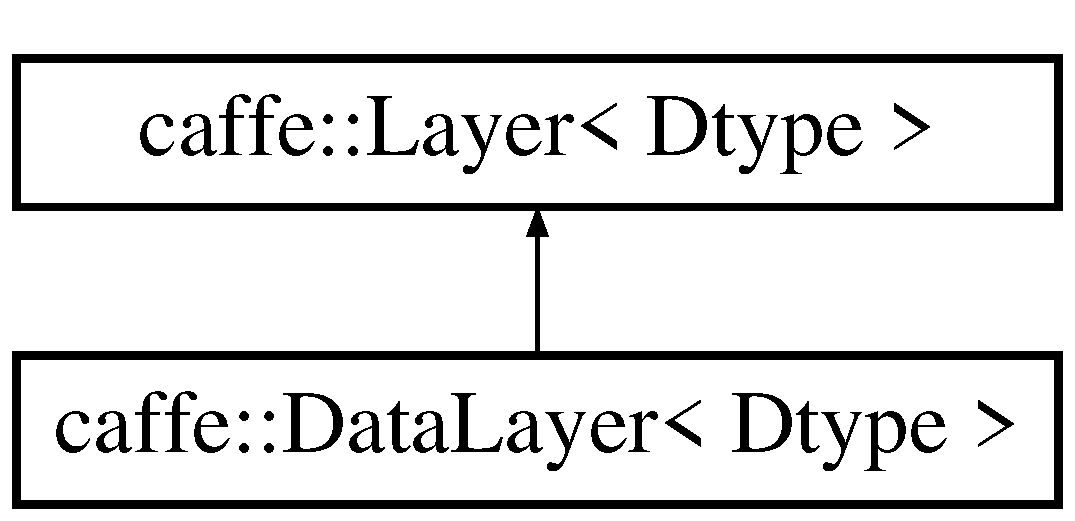
\includegraphics[height=2.000000cm]{classcaffe_1_1_data_layer}
\end{center}
\end{figure}
\subsection*{Public Member Functions}
\begin{DoxyCompactItemize}
\item 
\hyperlink{classcaffe_1_1_data_layer_a55d92ba6737e695551eca610868f1fae}{Data\+Layer} (const Layer\+Parameter \&param)
\item 
virtual \hyperlink{classcaffe_1_1_data_layer_a4fb35db42c400f2503dac67ebbbf21bb}{$\sim$\+Data\+Layer} ()
\item 
virtual void \hyperlink{classcaffe_1_1_data_layer_a157c4ee7c0a8c1b961a80c9a6432c7ea}{Set\+Up} (const vector$<$ \hyperlink{classcaffe_1_1_blob}{Blob}$<$ Dtype $>$ $\ast$ $>$ \&bottom, vector$<$ \hyperlink{classcaffe_1_1_blob}{Blob}$<$ Dtype $>$ $\ast$ $>$ $\ast$top)
\end{DoxyCompactItemize}
\subsection*{Protected Member Functions}
\begin{DoxyCompactItemize}
\item 
virtual Dtype \hyperlink{classcaffe_1_1_data_layer_a35e60c6ea0e3b8b57671d42853e956c3}{Forward\+\_\+cpu} (const vector$<$ \hyperlink{classcaffe_1_1_blob}{Blob}$<$ Dtype $>$ $\ast$ $>$ \&bottom, vector$<$ \hyperlink{classcaffe_1_1_blob}{Blob}$<$ Dtype $>$ $\ast$ $>$ $\ast$top)
\item 
virtual Dtype \hyperlink{classcaffe_1_1_data_layer_ae94ad93e1ad35123624e0aba0a2f03c6}{Forward\+\_\+gpu} (const vector$<$ \hyperlink{classcaffe_1_1_blob}{Blob}$<$ Dtype $>$ $\ast$ $>$ \&bottom, vector$<$ \hyperlink{classcaffe_1_1_blob}{Blob}$<$ Dtype $>$ $\ast$ $>$ $\ast$top)
\item 
virtual void \hyperlink{classcaffe_1_1_data_layer_a4b58dd246c6d1d1c3950f8c344c8b5ac}{Backward\+\_\+cpu} (const vector$<$ \hyperlink{classcaffe_1_1_blob}{Blob}$<$ Dtype $>$ $\ast$ $>$ \&top, const bool propagate\+\_\+down, vector$<$ \hyperlink{classcaffe_1_1_blob}{Blob}$<$ Dtype $>$ $\ast$ $>$ $\ast$bottom)
\item 
virtual void \hyperlink{classcaffe_1_1_data_layer_a7d9d69b7d2fbb6635b677ade18d9d8be}{Backward\+\_\+gpu} (const vector$<$ \hyperlink{classcaffe_1_1_blob}{Blob}$<$ Dtype $>$ $\ast$ $>$ \&top, const bool propagate\+\_\+down, vector$<$ \hyperlink{classcaffe_1_1_blob}{Blob}$<$ Dtype $>$ $\ast$ $>$ $\ast$bottom)
\item 
virtual void \hyperlink{classcaffe_1_1_data_layer_a54227e2ee704bfa023013f8d3d42410e}{Create\+Prefetch\+Thread} ()
\item 
virtual void \hyperlink{classcaffe_1_1_data_layer_af74ca774cacdf52bcdd70046c4619fc8}{Join\+Prefetch\+Thread} ()
\item 
virtual unsigned int \hyperlink{classcaffe_1_1_data_layer_ab273ed9ed64cd430b2d84308958ee531}{Prefetch\+Rand} ()
\end{DoxyCompactItemize}
\subsection*{Protected Attributes}
\begin{DoxyCompactItemize}
\item 
shared\+\_\+ptr$<$ \hyperlink{classcaffe_1_1_caffe_1_1_r_n_g}{Caffe\+::\+R\+N\+G} $>$ \hyperlink{classcaffe_1_1_data_layer_a1ec4389cc48a637748446900ccab7767}{prefetch\+\_\+rng\+\_\+}
\item 
shared\+\_\+ptr$<$ leveldb\+::\+D\+B $>$ \hyperlink{classcaffe_1_1_data_layer_a9287a92e591da10a3d6f38333aad301f}{db\+\_\+}
\item 
shared\+\_\+ptr$<$ leveldb\+::\+Iterator $>$ \hyperlink{classcaffe_1_1_data_layer_a5f02294c8b3cf2a31f4e97accf3a23dd}{iter\+\_\+}
\item 
int \hyperlink{classcaffe_1_1_data_layer_a33f86db700bff9553d05151c04a95e0d}{datum\+\_\+channels\+\_\+}
\item 
int \hyperlink{classcaffe_1_1_data_layer_a05b52e5bbe760b831728f1f0c0bed60b}{datum\+\_\+height\+\_\+}
\item 
int \hyperlink{classcaffe_1_1_data_layer_a87acabb37f849641efdcb605031dc352}{datum\+\_\+width\+\_\+}
\item 
int \hyperlink{classcaffe_1_1_data_layer_a9b2617e874504b7780584d869d461bf3}{datum\+\_\+size\+\_\+}
\item 
pthread\+\_\+t \hyperlink{classcaffe_1_1_data_layer_a62fda7f98477da13464f787e72be0b09}{thread\+\_\+}
\item 
shared\+\_\+ptr$<$ \hyperlink{classcaffe_1_1_blob}{Blob}$<$ Dtype $>$ $>$ \hyperlink{classcaffe_1_1_data_layer_a6c61442271fe47f944c2b07a794b4245}{prefetch\+\_\+data\+\_\+}
\item 
shared\+\_\+ptr$<$ \hyperlink{classcaffe_1_1_blob}{Blob}$<$ Dtype $>$ $>$ \hyperlink{classcaffe_1_1_data_layer_a3bd700fc3b186d60ce90329a57923830}{prefetch\+\_\+label\+\_\+}
\item 
\hyperlink{classcaffe_1_1_blob}{Blob}$<$ Dtype $>$ \hyperlink{classcaffe_1_1_data_layer_a83d1439647876032a72468a7a8c4b889}{data\+\_\+mean\+\_\+}
\item 
bool \hyperlink{classcaffe_1_1_data_layer_ae2d9349591a22759acfce89a3ff7908a}{output\+\_\+labels\+\_\+}
\item 
\hyperlink{classcaffe_1_1_caffe_ad2993dccc4a615c39259ed7f0d0e24e9}{Caffe\+::\+Phase} \hyperlink{classcaffe_1_1_data_layer_adf7d23050e73666ed3305715624599c2}{phase\+\_\+}
\end{DoxyCompactItemize}
\subsection*{Friends}
\begin{DoxyCompactItemize}
\item 
void $\ast$ \hyperlink{classcaffe_1_1_data_layer_a8771dd3f6476328a185ea02a3e9f6886}{Data\+Layer\+Prefetch} (void $\ast$layer\+\_\+pointer)
\end{DoxyCompactItemize}


\subsection{Constructor \& Destructor Documentation}
\hypertarget{classcaffe_1_1_data_layer_a55d92ba6737e695551eca610868f1fae}{\index{caffe\+::\+Data\+Layer@{caffe\+::\+Data\+Layer}!Data\+Layer@{Data\+Layer}}
\index{Data\+Layer@{Data\+Layer}!caffe\+::\+Data\+Layer@{caffe\+::\+Data\+Layer}}
\subsubsection[{Data\+Layer}]{\setlength{\rightskip}{0pt plus 5cm}template$<$typename Dtype $>$ {\bf caffe\+::\+Data\+Layer}$<$ Dtype $>$\+::{\bf Data\+Layer} (
\begin{DoxyParamCaption}
\item[{const Layer\+Parameter \&}]{param}
\end{DoxyParamCaption}
)\hspace{0.3cm}{\ttfamily [inline]}, {\ttfamily [explicit]}}}\label{classcaffe_1_1_data_layer_a55d92ba6737e695551eca610868f1fae}
\hypertarget{classcaffe_1_1_data_layer_a4fb35db42c400f2503dac67ebbbf21bb}{\index{caffe\+::\+Data\+Layer@{caffe\+::\+Data\+Layer}!````~Data\+Layer@{$\sim$\+Data\+Layer}}
\index{````~Data\+Layer@{$\sim$\+Data\+Layer}!caffe\+::\+Data\+Layer@{caffe\+::\+Data\+Layer}}
\subsubsection[{$\sim$\+Data\+Layer}]{\setlength{\rightskip}{0pt plus 5cm}template$<$typename Dtype $>$ {\bf caffe\+::\+Data\+Layer}$<$ Dtype $>$\+::$\sim${\bf Data\+Layer}$<$ Dtype $>$ (
\begin{DoxyParamCaption}
{}
\end{DoxyParamCaption}
)\hspace{0.3cm}{\ttfamily [virtual]}}}\label{classcaffe_1_1_data_layer_a4fb35db42c400f2503dac67ebbbf21bb}


\subsection{Member Function Documentation}
\hypertarget{classcaffe_1_1_data_layer_a4b58dd246c6d1d1c3950f8c344c8b5ac}{\index{caffe\+::\+Data\+Layer@{caffe\+::\+Data\+Layer}!Backward\+\_\+cpu@{Backward\+\_\+cpu}}
\index{Backward\+\_\+cpu@{Backward\+\_\+cpu}!caffe\+::\+Data\+Layer@{caffe\+::\+Data\+Layer}}
\subsubsection[{Backward\+\_\+cpu}]{\setlength{\rightskip}{0pt plus 5cm}template$<$typename Dtype $>$ virtual void {\bf caffe\+::\+Data\+Layer}$<$ Dtype $>$\+::Backward\+\_\+cpu (
\begin{DoxyParamCaption}
\item[{const vector$<$ {\bf Blob}$<$ Dtype $>$ $\ast$ $>$ \&}]{top, }
\item[{const bool}]{propagate\+\_\+down, }
\item[{vector$<$ {\bf Blob}$<$ Dtype $>$ $\ast$ $>$ $\ast$}]{bottom}
\end{DoxyParamCaption}
)\hspace{0.3cm}{\ttfamily [inline]}, {\ttfamily [protected]}, {\ttfamily [virtual]}}}\label{classcaffe_1_1_data_layer_a4b58dd246c6d1d1c3950f8c344c8b5ac}


Implements \hyperlink{classcaffe_1_1_layer_ac2d82011d076237c67997f63e7ee4b80}{caffe\+::\+Layer$<$ Dtype $>$}.

\hypertarget{classcaffe_1_1_data_layer_a7d9d69b7d2fbb6635b677ade18d9d8be}{\index{caffe\+::\+Data\+Layer@{caffe\+::\+Data\+Layer}!Backward\+\_\+gpu@{Backward\+\_\+gpu}}
\index{Backward\+\_\+gpu@{Backward\+\_\+gpu}!caffe\+::\+Data\+Layer@{caffe\+::\+Data\+Layer}}
\subsubsection[{Backward\+\_\+gpu}]{\setlength{\rightskip}{0pt plus 5cm}template$<$typename Dtype $>$ virtual void {\bf caffe\+::\+Data\+Layer}$<$ Dtype $>$\+::Backward\+\_\+gpu (
\begin{DoxyParamCaption}
\item[{const vector$<$ {\bf Blob}$<$ Dtype $>$ $\ast$ $>$ \&}]{top, }
\item[{const bool}]{propagate\+\_\+down, }
\item[{vector$<$ {\bf Blob}$<$ Dtype $>$ $\ast$ $>$ $\ast$}]{bottom}
\end{DoxyParamCaption}
)\hspace{0.3cm}{\ttfamily [inline]}, {\ttfamily [protected]}, {\ttfamily [virtual]}}}\label{classcaffe_1_1_data_layer_a7d9d69b7d2fbb6635b677ade18d9d8be}


Reimplemented from \hyperlink{classcaffe_1_1_layer_adf07ffe1f22d2fd2b1b0ff475ef5a64b}{caffe\+::\+Layer$<$ Dtype $>$}.

\hypertarget{classcaffe_1_1_data_layer_a54227e2ee704bfa023013f8d3d42410e}{\index{caffe\+::\+Data\+Layer@{caffe\+::\+Data\+Layer}!Create\+Prefetch\+Thread@{Create\+Prefetch\+Thread}}
\index{Create\+Prefetch\+Thread@{Create\+Prefetch\+Thread}!caffe\+::\+Data\+Layer@{caffe\+::\+Data\+Layer}}
\subsubsection[{Create\+Prefetch\+Thread}]{\setlength{\rightskip}{0pt plus 5cm}template$<$typename Dtype $>$ void {\bf caffe\+::\+Data\+Layer}$<$ Dtype $>$\+::Create\+Prefetch\+Thread (
\begin{DoxyParamCaption}
{}
\end{DoxyParamCaption}
)\hspace{0.3cm}{\ttfamily [protected]}, {\ttfamily [virtual]}}}\label{classcaffe_1_1_data_layer_a54227e2ee704bfa023013f8d3d42410e}
\hypertarget{classcaffe_1_1_data_layer_a35e60c6ea0e3b8b57671d42853e956c3}{\index{caffe\+::\+Data\+Layer@{caffe\+::\+Data\+Layer}!Forward\+\_\+cpu@{Forward\+\_\+cpu}}
\index{Forward\+\_\+cpu@{Forward\+\_\+cpu}!caffe\+::\+Data\+Layer@{caffe\+::\+Data\+Layer}}
\subsubsection[{Forward\+\_\+cpu}]{\setlength{\rightskip}{0pt plus 5cm}template$<$typename Dtype $>$ Dtype {\bf caffe\+::\+Data\+Layer}$<$ Dtype $>$\+::Forward\+\_\+cpu (
\begin{DoxyParamCaption}
\item[{const vector$<$ {\bf Blob}$<$ Dtype $>$ $\ast$ $>$ \&}]{bottom, }
\item[{vector$<$ {\bf Blob}$<$ Dtype $>$ $\ast$ $>$ $\ast$}]{top}
\end{DoxyParamCaption}
)\hspace{0.3cm}{\ttfamily [protected]}, {\ttfamily [virtual]}}}\label{classcaffe_1_1_data_layer_a35e60c6ea0e3b8b57671d42853e956c3}


Implements \hyperlink{classcaffe_1_1_layer_a8f7f61da3b8b3ca7f2394dee33873353}{caffe\+::\+Layer$<$ Dtype $>$}.

\hypertarget{classcaffe_1_1_data_layer_ae94ad93e1ad35123624e0aba0a2f03c6}{\index{caffe\+::\+Data\+Layer@{caffe\+::\+Data\+Layer}!Forward\+\_\+gpu@{Forward\+\_\+gpu}}
\index{Forward\+\_\+gpu@{Forward\+\_\+gpu}!caffe\+::\+Data\+Layer@{caffe\+::\+Data\+Layer}}
\subsubsection[{Forward\+\_\+gpu}]{\setlength{\rightskip}{0pt plus 5cm}template$<$typename Dtype $>$ Dtype {\bf caffe\+::\+Data\+Layer}$<$ Dtype $>$\+::Forward\+\_\+gpu (
\begin{DoxyParamCaption}
\item[{const vector$<$ {\bf Blob}$<$ Dtype $>$ $\ast$ $>$ \&}]{bottom, }
\item[{vector$<$ {\bf Blob}$<$ Dtype $>$ $\ast$ $>$ $\ast$}]{top}
\end{DoxyParamCaption}
)\hspace{0.3cm}{\ttfamily [protected]}, {\ttfamily [virtual]}}}\label{classcaffe_1_1_data_layer_ae94ad93e1ad35123624e0aba0a2f03c6}


Reimplemented from \hyperlink{classcaffe_1_1_layer_a2d78dbf5d8bc36928bd8f6fcfbafbcef}{caffe\+::\+Layer$<$ Dtype $>$}.

\hypertarget{classcaffe_1_1_data_layer_af74ca774cacdf52bcdd70046c4619fc8}{\index{caffe\+::\+Data\+Layer@{caffe\+::\+Data\+Layer}!Join\+Prefetch\+Thread@{Join\+Prefetch\+Thread}}
\index{Join\+Prefetch\+Thread@{Join\+Prefetch\+Thread}!caffe\+::\+Data\+Layer@{caffe\+::\+Data\+Layer}}
\subsubsection[{Join\+Prefetch\+Thread}]{\setlength{\rightskip}{0pt plus 5cm}template$<$typename Dtype $>$ void {\bf caffe\+::\+Data\+Layer}$<$ Dtype $>$\+::Join\+Prefetch\+Thread (
\begin{DoxyParamCaption}
{}
\end{DoxyParamCaption}
)\hspace{0.3cm}{\ttfamily [protected]}, {\ttfamily [virtual]}}}\label{classcaffe_1_1_data_layer_af74ca774cacdf52bcdd70046c4619fc8}
\hypertarget{classcaffe_1_1_data_layer_ab273ed9ed64cd430b2d84308958ee531}{\index{caffe\+::\+Data\+Layer@{caffe\+::\+Data\+Layer}!Prefetch\+Rand@{Prefetch\+Rand}}
\index{Prefetch\+Rand@{Prefetch\+Rand}!caffe\+::\+Data\+Layer@{caffe\+::\+Data\+Layer}}
\subsubsection[{Prefetch\+Rand}]{\setlength{\rightskip}{0pt plus 5cm}template$<$typename Dtype $>$ unsigned int {\bf caffe\+::\+Data\+Layer}$<$ Dtype $>$\+::Prefetch\+Rand (
\begin{DoxyParamCaption}
{}
\end{DoxyParamCaption}
)\hspace{0.3cm}{\ttfamily [protected]}, {\ttfamily [virtual]}}}\label{classcaffe_1_1_data_layer_ab273ed9ed64cd430b2d84308958ee531}
\hypertarget{classcaffe_1_1_data_layer_a157c4ee7c0a8c1b961a80c9a6432c7ea}{\index{caffe\+::\+Data\+Layer@{caffe\+::\+Data\+Layer}!Set\+Up@{Set\+Up}}
\index{Set\+Up@{Set\+Up}!caffe\+::\+Data\+Layer@{caffe\+::\+Data\+Layer}}
\subsubsection[{Set\+Up}]{\setlength{\rightskip}{0pt plus 5cm}template$<$typename Dtype $>$ void {\bf caffe\+::\+Data\+Layer}$<$ Dtype $>$\+::Set\+Up (
\begin{DoxyParamCaption}
\item[{const vector$<$ {\bf Blob}$<$ Dtype $>$ $\ast$ $>$ \&}]{bottom, }
\item[{vector$<$ {\bf Blob}$<$ Dtype $>$ $\ast$ $>$ $\ast$}]{top}
\end{DoxyParamCaption}
)\hspace{0.3cm}{\ttfamily [virtual]}}}\label{classcaffe_1_1_data_layer_a157c4ee7c0a8c1b961a80c9a6432c7ea}


Implements \hyperlink{classcaffe_1_1_layer_abd13c6489c13953b4fbcfcf6880835d0}{caffe\+::\+Layer$<$ Dtype $>$}.



\subsection{Friends And Related Function Documentation}
\hypertarget{classcaffe_1_1_data_layer_a8771dd3f6476328a185ea02a3e9f6886}{\index{caffe\+::\+Data\+Layer@{caffe\+::\+Data\+Layer}!Data\+Layer\+Prefetch@{Data\+Layer\+Prefetch}}
\index{Data\+Layer\+Prefetch@{Data\+Layer\+Prefetch}!caffe\+::\+Data\+Layer@{caffe\+::\+Data\+Layer}}
\subsubsection[{Data\+Layer\+Prefetch}]{\setlength{\rightskip}{0pt plus 5cm}template$<$typename Dtype $>$ void$\ast$ Data\+Layer\+Prefetch (
\begin{DoxyParamCaption}
\item[{void $\ast$}]{layer\+\_\+pointer}
\end{DoxyParamCaption}
)\hspace{0.3cm}{\ttfamily [friend]}}}\label{classcaffe_1_1_data_layer_a8771dd3f6476328a185ea02a3e9f6886}


\subsection{Member Data Documentation}
\hypertarget{classcaffe_1_1_data_layer_a83d1439647876032a72468a7a8c4b889}{\index{caffe\+::\+Data\+Layer@{caffe\+::\+Data\+Layer}!data\+\_\+mean\+\_\+@{data\+\_\+mean\+\_\+}}
\index{data\+\_\+mean\+\_\+@{data\+\_\+mean\+\_\+}!caffe\+::\+Data\+Layer@{caffe\+::\+Data\+Layer}}
\subsubsection[{data\+\_\+mean\+\_\+}]{\setlength{\rightskip}{0pt plus 5cm}template$<$typename Dtype $>$ {\bf Blob}$<$Dtype$>$ {\bf caffe\+::\+Data\+Layer}$<$ Dtype $>$\+::data\+\_\+mean\+\_\+\hspace{0.3cm}{\ttfamily [protected]}}}\label{classcaffe_1_1_data_layer_a83d1439647876032a72468a7a8c4b889}
\hypertarget{classcaffe_1_1_data_layer_a33f86db700bff9553d05151c04a95e0d}{\index{caffe\+::\+Data\+Layer@{caffe\+::\+Data\+Layer}!datum\+\_\+channels\+\_\+@{datum\+\_\+channels\+\_\+}}
\index{datum\+\_\+channels\+\_\+@{datum\+\_\+channels\+\_\+}!caffe\+::\+Data\+Layer@{caffe\+::\+Data\+Layer}}
\subsubsection[{datum\+\_\+channels\+\_\+}]{\setlength{\rightskip}{0pt plus 5cm}template$<$typename Dtype $>$ int {\bf caffe\+::\+Data\+Layer}$<$ Dtype $>$\+::datum\+\_\+channels\+\_\+\hspace{0.3cm}{\ttfamily [protected]}}}\label{classcaffe_1_1_data_layer_a33f86db700bff9553d05151c04a95e0d}
\hypertarget{classcaffe_1_1_data_layer_a05b52e5bbe760b831728f1f0c0bed60b}{\index{caffe\+::\+Data\+Layer@{caffe\+::\+Data\+Layer}!datum\+\_\+height\+\_\+@{datum\+\_\+height\+\_\+}}
\index{datum\+\_\+height\+\_\+@{datum\+\_\+height\+\_\+}!caffe\+::\+Data\+Layer@{caffe\+::\+Data\+Layer}}
\subsubsection[{datum\+\_\+height\+\_\+}]{\setlength{\rightskip}{0pt plus 5cm}template$<$typename Dtype $>$ int {\bf caffe\+::\+Data\+Layer}$<$ Dtype $>$\+::datum\+\_\+height\+\_\+\hspace{0.3cm}{\ttfamily [protected]}}}\label{classcaffe_1_1_data_layer_a05b52e5bbe760b831728f1f0c0bed60b}
\hypertarget{classcaffe_1_1_data_layer_a9b2617e874504b7780584d869d461bf3}{\index{caffe\+::\+Data\+Layer@{caffe\+::\+Data\+Layer}!datum\+\_\+size\+\_\+@{datum\+\_\+size\+\_\+}}
\index{datum\+\_\+size\+\_\+@{datum\+\_\+size\+\_\+}!caffe\+::\+Data\+Layer@{caffe\+::\+Data\+Layer}}
\subsubsection[{datum\+\_\+size\+\_\+}]{\setlength{\rightskip}{0pt plus 5cm}template$<$typename Dtype $>$ int {\bf caffe\+::\+Data\+Layer}$<$ Dtype $>$\+::datum\+\_\+size\+\_\+\hspace{0.3cm}{\ttfamily [protected]}}}\label{classcaffe_1_1_data_layer_a9b2617e874504b7780584d869d461bf3}
\hypertarget{classcaffe_1_1_data_layer_a87acabb37f849641efdcb605031dc352}{\index{caffe\+::\+Data\+Layer@{caffe\+::\+Data\+Layer}!datum\+\_\+width\+\_\+@{datum\+\_\+width\+\_\+}}
\index{datum\+\_\+width\+\_\+@{datum\+\_\+width\+\_\+}!caffe\+::\+Data\+Layer@{caffe\+::\+Data\+Layer}}
\subsubsection[{datum\+\_\+width\+\_\+}]{\setlength{\rightskip}{0pt plus 5cm}template$<$typename Dtype $>$ int {\bf caffe\+::\+Data\+Layer}$<$ Dtype $>$\+::datum\+\_\+width\+\_\+\hspace{0.3cm}{\ttfamily [protected]}}}\label{classcaffe_1_1_data_layer_a87acabb37f849641efdcb605031dc352}
\hypertarget{classcaffe_1_1_data_layer_a9287a92e591da10a3d6f38333aad301f}{\index{caffe\+::\+Data\+Layer@{caffe\+::\+Data\+Layer}!db\+\_\+@{db\+\_\+}}
\index{db\+\_\+@{db\+\_\+}!caffe\+::\+Data\+Layer@{caffe\+::\+Data\+Layer}}
\subsubsection[{db\+\_\+}]{\setlength{\rightskip}{0pt plus 5cm}template$<$typename Dtype $>$ shared\+\_\+ptr$<$leveldb\+::\+D\+B$>$ {\bf caffe\+::\+Data\+Layer}$<$ Dtype $>$\+::db\+\_\+\hspace{0.3cm}{\ttfamily [protected]}}}\label{classcaffe_1_1_data_layer_a9287a92e591da10a3d6f38333aad301f}
\hypertarget{classcaffe_1_1_data_layer_a5f02294c8b3cf2a31f4e97accf3a23dd}{\index{caffe\+::\+Data\+Layer@{caffe\+::\+Data\+Layer}!iter\+\_\+@{iter\+\_\+}}
\index{iter\+\_\+@{iter\+\_\+}!caffe\+::\+Data\+Layer@{caffe\+::\+Data\+Layer}}
\subsubsection[{iter\+\_\+}]{\setlength{\rightskip}{0pt plus 5cm}template$<$typename Dtype $>$ shared\+\_\+ptr$<$leveldb\+::\+Iterator$>$ {\bf caffe\+::\+Data\+Layer}$<$ Dtype $>$\+::iter\+\_\+\hspace{0.3cm}{\ttfamily [protected]}}}\label{classcaffe_1_1_data_layer_a5f02294c8b3cf2a31f4e97accf3a23dd}
\hypertarget{classcaffe_1_1_data_layer_ae2d9349591a22759acfce89a3ff7908a}{\index{caffe\+::\+Data\+Layer@{caffe\+::\+Data\+Layer}!output\+\_\+labels\+\_\+@{output\+\_\+labels\+\_\+}}
\index{output\+\_\+labels\+\_\+@{output\+\_\+labels\+\_\+}!caffe\+::\+Data\+Layer@{caffe\+::\+Data\+Layer}}
\subsubsection[{output\+\_\+labels\+\_\+}]{\setlength{\rightskip}{0pt plus 5cm}template$<$typename Dtype $>$ bool {\bf caffe\+::\+Data\+Layer}$<$ Dtype $>$\+::output\+\_\+labels\+\_\+\hspace{0.3cm}{\ttfamily [protected]}}}\label{classcaffe_1_1_data_layer_ae2d9349591a22759acfce89a3ff7908a}
\hypertarget{classcaffe_1_1_data_layer_adf7d23050e73666ed3305715624599c2}{\index{caffe\+::\+Data\+Layer@{caffe\+::\+Data\+Layer}!phase\+\_\+@{phase\+\_\+}}
\index{phase\+\_\+@{phase\+\_\+}!caffe\+::\+Data\+Layer@{caffe\+::\+Data\+Layer}}
\subsubsection[{phase\+\_\+}]{\setlength{\rightskip}{0pt plus 5cm}template$<$typename Dtype $>$ {\bf Caffe\+::\+Phase} {\bf caffe\+::\+Data\+Layer}$<$ Dtype $>$\+::phase\+\_\+\hspace{0.3cm}{\ttfamily [protected]}}}\label{classcaffe_1_1_data_layer_adf7d23050e73666ed3305715624599c2}
\hypertarget{classcaffe_1_1_data_layer_a6c61442271fe47f944c2b07a794b4245}{\index{caffe\+::\+Data\+Layer@{caffe\+::\+Data\+Layer}!prefetch\+\_\+data\+\_\+@{prefetch\+\_\+data\+\_\+}}
\index{prefetch\+\_\+data\+\_\+@{prefetch\+\_\+data\+\_\+}!caffe\+::\+Data\+Layer@{caffe\+::\+Data\+Layer}}
\subsubsection[{prefetch\+\_\+data\+\_\+}]{\setlength{\rightskip}{0pt plus 5cm}template$<$typename Dtype $>$ shared\+\_\+ptr$<${\bf Blob}$<$Dtype$>$ $>$ {\bf caffe\+::\+Data\+Layer}$<$ Dtype $>$\+::prefetch\+\_\+data\+\_\+\hspace{0.3cm}{\ttfamily [protected]}}}\label{classcaffe_1_1_data_layer_a6c61442271fe47f944c2b07a794b4245}
\hypertarget{classcaffe_1_1_data_layer_a3bd700fc3b186d60ce90329a57923830}{\index{caffe\+::\+Data\+Layer@{caffe\+::\+Data\+Layer}!prefetch\+\_\+label\+\_\+@{prefetch\+\_\+label\+\_\+}}
\index{prefetch\+\_\+label\+\_\+@{prefetch\+\_\+label\+\_\+}!caffe\+::\+Data\+Layer@{caffe\+::\+Data\+Layer}}
\subsubsection[{prefetch\+\_\+label\+\_\+}]{\setlength{\rightskip}{0pt plus 5cm}template$<$typename Dtype $>$ shared\+\_\+ptr$<${\bf Blob}$<$Dtype$>$ $>$ {\bf caffe\+::\+Data\+Layer}$<$ Dtype $>$\+::prefetch\+\_\+label\+\_\+\hspace{0.3cm}{\ttfamily [protected]}}}\label{classcaffe_1_1_data_layer_a3bd700fc3b186d60ce90329a57923830}
\hypertarget{classcaffe_1_1_data_layer_a1ec4389cc48a637748446900ccab7767}{\index{caffe\+::\+Data\+Layer@{caffe\+::\+Data\+Layer}!prefetch\+\_\+rng\+\_\+@{prefetch\+\_\+rng\+\_\+}}
\index{prefetch\+\_\+rng\+\_\+@{prefetch\+\_\+rng\+\_\+}!caffe\+::\+Data\+Layer@{caffe\+::\+Data\+Layer}}
\subsubsection[{prefetch\+\_\+rng\+\_\+}]{\setlength{\rightskip}{0pt plus 5cm}template$<$typename Dtype $>$ shared\+\_\+ptr$<${\bf Caffe\+::\+R\+N\+G}$>$ {\bf caffe\+::\+Data\+Layer}$<$ Dtype $>$\+::prefetch\+\_\+rng\+\_\+\hspace{0.3cm}{\ttfamily [protected]}}}\label{classcaffe_1_1_data_layer_a1ec4389cc48a637748446900ccab7767}
\hypertarget{classcaffe_1_1_data_layer_a62fda7f98477da13464f787e72be0b09}{\index{caffe\+::\+Data\+Layer@{caffe\+::\+Data\+Layer}!thread\+\_\+@{thread\+\_\+}}
\index{thread\+\_\+@{thread\+\_\+}!caffe\+::\+Data\+Layer@{caffe\+::\+Data\+Layer}}
\subsubsection[{thread\+\_\+}]{\setlength{\rightskip}{0pt plus 5cm}template$<$typename Dtype $>$ pthread\+\_\+t {\bf caffe\+::\+Data\+Layer}$<$ Dtype $>$\+::thread\+\_\+\hspace{0.3cm}{\ttfamily [protected]}}}\label{classcaffe_1_1_data_layer_a62fda7f98477da13464f787e72be0b09}


The documentation for this class was generated from the following files\+:\begin{DoxyCompactItemize}
\item 
include/caffe/\hyperlink{vision__layers_8hpp}{vision\+\_\+layers.\+hpp}\item 
src/caffe/layers/\hyperlink{data__layer_8cpp}{data\+\_\+layer.\+cpp}\item 
src/caffe/layers/\hyperlink{data__layer_8cu}{data\+\_\+layer.\+cu}\end{DoxyCompactItemize}

\hypertarget{classcaffe_1_1_data_layer_test}{\section{caffe\+:\+:Data\+Layer\+Test$<$ Dtype $>$ Class Template Reference}
\label{classcaffe_1_1_data_layer_test}\index{caffe\+::\+Data\+Layer\+Test$<$ Dtype $>$@{caffe\+::\+Data\+Layer\+Test$<$ Dtype $>$}}
}
Inheritance diagram for caffe\+:\+:Data\+Layer\+Test$<$ Dtype $>$\+:\begin{figure}[H]
\begin{center}
\leavevmode
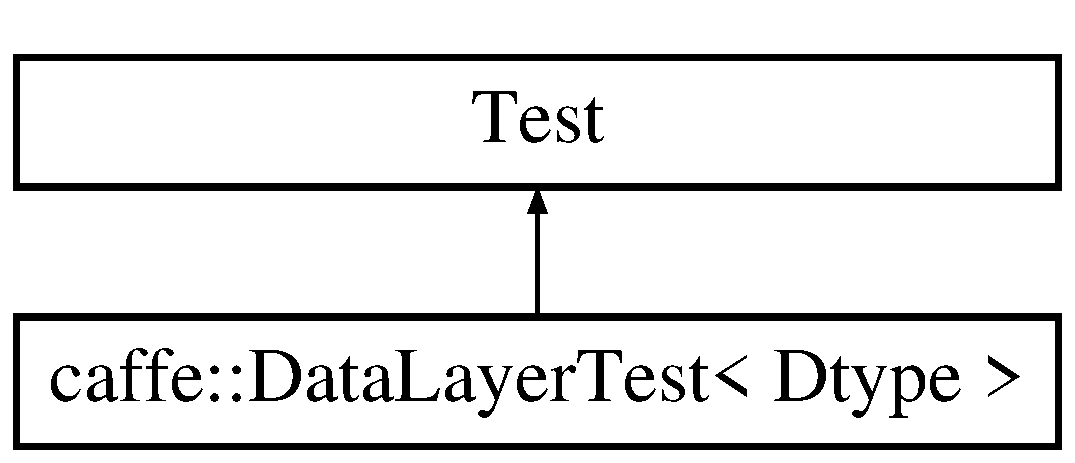
\includegraphics[height=2.000000cm]{classcaffe_1_1_data_layer_test}
\end{center}
\end{figure}
\subsection*{Protected Member Functions}
\begin{DoxyCompactItemize}
\item 
\hyperlink{classcaffe_1_1_data_layer_test_ac4d32d60646a6b4f362ad9a934008f93}{Data\+Layer\+Test} ()
\item 
virtual void \hyperlink{classcaffe_1_1_data_layer_test_a67b66edfd71f6e3d7a5c0cda35b08d8a}{Set\+Up} ()
\item 
void \hyperlink{classcaffe_1_1_data_layer_test_a7877b2f9d2cb43b3afc867336562e308}{Fill\+Level\+D\+B} (const bool unique\+\_\+pixels)
\item 
virtual \hyperlink{classcaffe_1_1_data_layer_test_ab57a2320076b2d08574b9aa43091397f}{$\sim$\+Data\+Layer\+Test} ()
\end{DoxyCompactItemize}
\subsection*{Protected Attributes}
\begin{DoxyCompactItemize}
\item 
shared\+\_\+ptr$<$ string $>$ \hyperlink{classcaffe_1_1_data_layer_test_a96918f4c6321111e66d795f4341fd656}{filename\+\_\+}
\item 
\hyperlink{classcaffe_1_1_blob}{Blob}$<$ Dtype $>$ $\ast$const \hyperlink{classcaffe_1_1_data_layer_test_a5810c2d8664d032fd3b96dd9eeac24d8}{blob\+\_\+top\+\_\+data\+\_\+}
\item 
\hyperlink{classcaffe_1_1_blob}{Blob}$<$ Dtype $>$ $\ast$const \hyperlink{classcaffe_1_1_data_layer_test_a56fd4aed58fbf6c4a24373e9df1d732a}{blob\+\_\+top\+\_\+label\+\_\+}
\item 
vector$<$ \hyperlink{classcaffe_1_1_blob}{Blob}$<$ Dtype $>$ $\ast$ $>$ \hyperlink{classcaffe_1_1_data_layer_test_af547e93d91fa20aef8d1026b4b006a86}{blob\+\_\+bottom\+\_\+vec\+\_\+}
\item 
vector$<$ \hyperlink{classcaffe_1_1_blob}{Blob}$<$ Dtype $>$ $\ast$ $>$ \hyperlink{classcaffe_1_1_data_layer_test_a591c04139193a11697a051889cddf83d}{blob\+\_\+top\+\_\+vec\+\_\+}
\item 
int \hyperlink{classcaffe_1_1_data_layer_test_acf77bf66c5261af404bc1aa28fc3e7d0}{seed\+\_\+}
\end{DoxyCompactItemize}


\subsection{Constructor \& Destructor Documentation}
\hypertarget{classcaffe_1_1_data_layer_test_ac4d32d60646a6b4f362ad9a934008f93}{\index{caffe\+::\+Data\+Layer\+Test@{caffe\+::\+Data\+Layer\+Test}!Data\+Layer\+Test@{Data\+Layer\+Test}}
\index{Data\+Layer\+Test@{Data\+Layer\+Test}!caffe\+::\+Data\+Layer\+Test@{caffe\+::\+Data\+Layer\+Test}}
\subsubsection[{Data\+Layer\+Test}]{\setlength{\rightskip}{0pt plus 5cm}template$<$typename Dtype $>$ {\bf caffe\+::\+Data\+Layer\+Test}$<$ Dtype $>$\+::{\bf Data\+Layer\+Test} (
\begin{DoxyParamCaption}
{}
\end{DoxyParamCaption}
)\hspace{0.3cm}{\ttfamily [inline]}, {\ttfamily [protected]}}}\label{classcaffe_1_1_data_layer_test_ac4d32d60646a6b4f362ad9a934008f93}
\hypertarget{classcaffe_1_1_data_layer_test_ab57a2320076b2d08574b9aa43091397f}{\index{caffe\+::\+Data\+Layer\+Test@{caffe\+::\+Data\+Layer\+Test}!````~Data\+Layer\+Test@{$\sim$\+Data\+Layer\+Test}}
\index{````~Data\+Layer\+Test@{$\sim$\+Data\+Layer\+Test}!caffe\+::\+Data\+Layer\+Test@{caffe\+::\+Data\+Layer\+Test}}
\subsubsection[{$\sim$\+Data\+Layer\+Test}]{\setlength{\rightskip}{0pt plus 5cm}template$<$typename Dtype $>$ virtual {\bf caffe\+::\+Data\+Layer\+Test}$<$ Dtype $>$\+::$\sim${\bf Data\+Layer\+Test} (
\begin{DoxyParamCaption}
{}
\end{DoxyParamCaption}
)\hspace{0.3cm}{\ttfamily [inline]}, {\ttfamily [protected]}, {\ttfamily [virtual]}}}\label{classcaffe_1_1_data_layer_test_ab57a2320076b2d08574b9aa43091397f}


\subsection{Member Function Documentation}
\hypertarget{classcaffe_1_1_data_layer_test_a7877b2f9d2cb43b3afc867336562e308}{\index{caffe\+::\+Data\+Layer\+Test@{caffe\+::\+Data\+Layer\+Test}!Fill\+Level\+D\+B@{Fill\+Level\+D\+B}}
\index{Fill\+Level\+D\+B@{Fill\+Level\+D\+B}!caffe\+::\+Data\+Layer\+Test@{caffe\+::\+Data\+Layer\+Test}}
\subsubsection[{Fill\+Level\+D\+B}]{\setlength{\rightskip}{0pt plus 5cm}template$<$typename Dtype $>$ void {\bf caffe\+::\+Data\+Layer\+Test}$<$ Dtype $>$\+::Fill\+Level\+D\+B (
\begin{DoxyParamCaption}
\item[{const bool}]{unique\+\_\+pixels}
\end{DoxyParamCaption}
)\hspace{0.3cm}{\ttfamily [inline]}, {\ttfamily [protected]}}}\label{classcaffe_1_1_data_layer_test_a7877b2f9d2cb43b3afc867336562e308}
\hypertarget{classcaffe_1_1_data_layer_test_a67b66edfd71f6e3d7a5c0cda35b08d8a}{\index{caffe\+::\+Data\+Layer\+Test@{caffe\+::\+Data\+Layer\+Test}!Set\+Up@{Set\+Up}}
\index{Set\+Up@{Set\+Up}!caffe\+::\+Data\+Layer\+Test@{caffe\+::\+Data\+Layer\+Test}}
\subsubsection[{Set\+Up}]{\setlength{\rightskip}{0pt plus 5cm}template$<$typename Dtype $>$ virtual void {\bf caffe\+::\+Data\+Layer\+Test}$<$ Dtype $>$\+::Set\+Up (
\begin{DoxyParamCaption}
{}
\end{DoxyParamCaption}
)\hspace{0.3cm}{\ttfamily [inline]}, {\ttfamily [protected]}, {\ttfamily [virtual]}}}\label{classcaffe_1_1_data_layer_test_a67b66edfd71f6e3d7a5c0cda35b08d8a}


\subsection{Member Data Documentation}
\hypertarget{classcaffe_1_1_data_layer_test_af547e93d91fa20aef8d1026b4b006a86}{\index{caffe\+::\+Data\+Layer\+Test@{caffe\+::\+Data\+Layer\+Test}!blob\+\_\+bottom\+\_\+vec\+\_\+@{blob\+\_\+bottom\+\_\+vec\+\_\+}}
\index{blob\+\_\+bottom\+\_\+vec\+\_\+@{blob\+\_\+bottom\+\_\+vec\+\_\+}!caffe\+::\+Data\+Layer\+Test@{caffe\+::\+Data\+Layer\+Test}}
\subsubsection[{blob\+\_\+bottom\+\_\+vec\+\_\+}]{\setlength{\rightskip}{0pt plus 5cm}template$<$typename Dtype $>$ vector$<${\bf Blob}$<$Dtype$>$$\ast$$>$ {\bf caffe\+::\+Data\+Layer\+Test}$<$ Dtype $>$\+::blob\+\_\+bottom\+\_\+vec\+\_\+\hspace{0.3cm}{\ttfamily [protected]}}}\label{classcaffe_1_1_data_layer_test_af547e93d91fa20aef8d1026b4b006a86}
\hypertarget{classcaffe_1_1_data_layer_test_a5810c2d8664d032fd3b96dd9eeac24d8}{\index{caffe\+::\+Data\+Layer\+Test@{caffe\+::\+Data\+Layer\+Test}!blob\+\_\+top\+\_\+data\+\_\+@{blob\+\_\+top\+\_\+data\+\_\+}}
\index{blob\+\_\+top\+\_\+data\+\_\+@{blob\+\_\+top\+\_\+data\+\_\+}!caffe\+::\+Data\+Layer\+Test@{caffe\+::\+Data\+Layer\+Test}}
\subsubsection[{blob\+\_\+top\+\_\+data\+\_\+}]{\setlength{\rightskip}{0pt plus 5cm}template$<$typename Dtype $>$ {\bf Blob}$<$Dtype$>$$\ast$ const {\bf caffe\+::\+Data\+Layer\+Test}$<$ Dtype $>$\+::blob\+\_\+top\+\_\+data\+\_\+\hspace{0.3cm}{\ttfamily [protected]}}}\label{classcaffe_1_1_data_layer_test_a5810c2d8664d032fd3b96dd9eeac24d8}
\hypertarget{classcaffe_1_1_data_layer_test_a56fd4aed58fbf6c4a24373e9df1d732a}{\index{caffe\+::\+Data\+Layer\+Test@{caffe\+::\+Data\+Layer\+Test}!blob\+\_\+top\+\_\+label\+\_\+@{blob\+\_\+top\+\_\+label\+\_\+}}
\index{blob\+\_\+top\+\_\+label\+\_\+@{blob\+\_\+top\+\_\+label\+\_\+}!caffe\+::\+Data\+Layer\+Test@{caffe\+::\+Data\+Layer\+Test}}
\subsubsection[{blob\+\_\+top\+\_\+label\+\_\+}]{\setlength{\rightskip}{0pt plus 5cm}template$<$typename Dtype $>$ {\bf Blob}$<$Dtype$>$$\ast$ const {\bf caffe\+::\+Data\+Layer\+Test}$<$ Dtype $>$\+::blob\+\_\+top\+\_\+label\+\_\+\hspace{0.3cm}{\ttfamily [protected]}}}\label{classcaffe_1_1_data_layer_test_a56fd4aed58fbf6c4a24373e9df1d732a}
\hypertarget{classcaffe_1_1_data_layer_test_a591c04139193a11697a051889cddf83d}{\index{caffe\+::\+Data\+Layer\+Test@{caffe\+::\+Data\+Layer\+Test}!blob\+\_\+top\+\_\+vec\+\_\+@{blob\+\_\+top\+\_\+vec\+\_\+}}
\index{blob\+\_\+top\+\_\+vec\+\_\+@{blob\+\_\+top\+\_\+vec\+\_\+}!caffe\+::\+Data\+Layer\+Test@{caffe\+::\+Data\+Layer\+Test}}
\subsubsection[{blob\+\_\+top\+\_\+vec\+\_\+}]{\setlength{\rightskip}{0pt plus 5cm}template$<$typename Dtype $>$ vector$<${\bf Blob}$<$Dtype$>$$\ast$$>$ {\bf caffe\+::\+Data\+Layer\+Test}$<$ Dtype $>$\+::blob\+\_\+top\+\_\+vec\+\_\+\hspace{0.3cm}{\ttfamily [protected]}}}\label{classcaffe_1_1_data_layer_test_a591c04139193a11697a051889cddf83d}
\hypertarget{classcaffe_1_1_data_layer_test_a96918f4c6321111e66d795f4341fd656}{\index{caffe\+::\+Data\+Layer\+Test@{caffe\+::\+Data\+Layer\+Test}!filename\+\_\+@{filename\+\_\+}}
\index{filename\+\_\+@{filename\+\_\+}!caffe\+::\+Data\+Layer\+Test@{caffe\+::\+Data\+Layer\+Test}}
\subsubsection[{filename\+\_\+}]{\setlength{\rightskip}{0pt plus 5cm}template$<$typename Dtype $>$ shared\+\_\+ptr$<$string$>$ {\bf caffe\+::\+Data\+Layer\+Test}$<$ Dtype $>$\+::filename\+\_\+\hspace{0.3cm}{\ttfamily [protected]}}}\label{classcaffe_1_1_data_layer_test_a96918f4c6321111e66d795f4341fd656}
\hypertarget{classcaffe_1_1_data_layer_test_acf77bf66c5261af404bc1aa28fc3e7d0}{\index{caffe\+::\+Data\+Layer\+Test@{caffe\+::\+Data\+Layer\+Test}!seed\+\_\+@{seed\+\_\+}}
\index{seed\+\_\+@{seed\+\_\+}!caffe\+::\+Data\+Layer\+Test@{caffe\+::\+Data\+Layer\+Test}}
\subsubsection[{seed\+\_\+}]{\setlength{\rightskip}{0pt plus 5cm}template$<$typename Dtype $>$ int {\bf caffe\+::\+Data\+Layer\+Test}$<$ Dtype $>$\+::seed\+\_\+\hspace{0.3cm}{\ttfamily [protected]}}}\label{classcaffe_1_1_data_layer_test_acf77bf66c5261af404bc1aa28fc3e7d0}


The documentation for this class was generated from the following file\+:\begin{DoxyCompactItemize}
\item 
src/caffe/test/\hyperlink{test__data__layer_8cpp}{test\+\_\+data\+\_\+layer.\+cpp}\end{DoxyCompactItemize}

\hypertarget{classcaffe_1_1_dropout_layer}{\section{caffe\+:\+:Dropout\+Layer$<$ Dtype $>$ Class Template Reference}
\label{classcaffe_1_1_dropout_layer}\index{caffe\+::\+Dropout\+Layer$<$ Dtype $>$@{caffe\+::\+Dropout\+Layer$<$ Dtype $>$}}
}


{\ttfamily \#include $<$vision\+\_\+layers.\+hpp$>$}

Inheritance diagram for caffe\+:\+:Dropout\+Layer$<$ Dtype $>$\+:\begin{figure}[H]
\begin{center}
\leavevmode
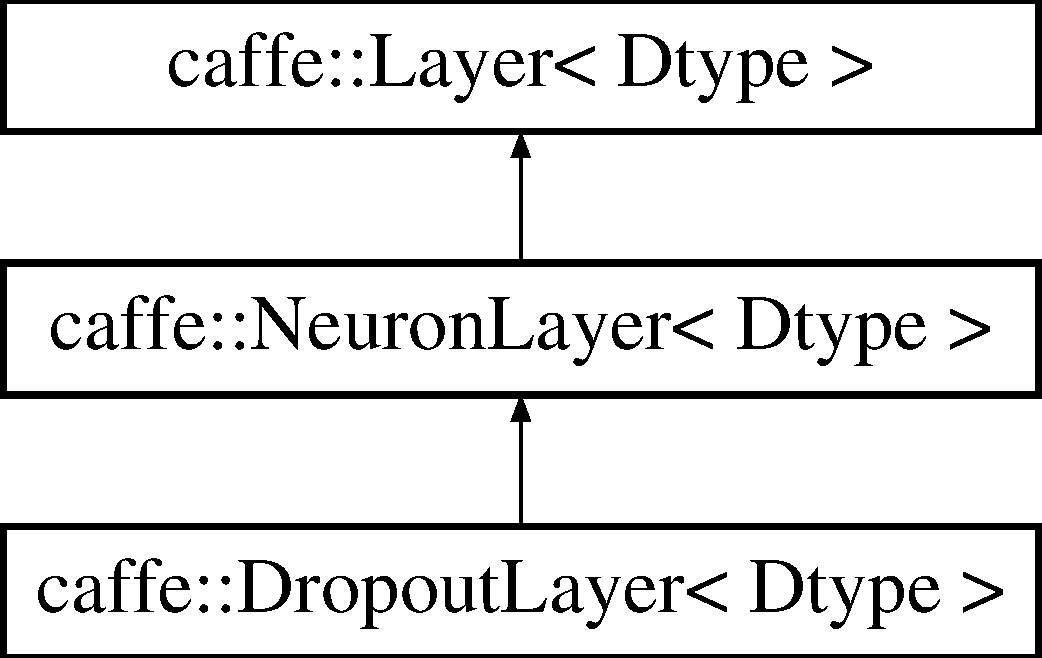
\includegraphics[height=3.000000cm]{classcaffe_1_1_dropout_layer}
\end{center}
\end{figure}
\subsection*{Public Member Functions}
\begin{DoxyCompactItemize}
\item 
\hyperlink{classcaffe_1_1_dropout_layer_a24cbddd4699b102a9555d3b8013c16d0}{Dropout\+Layer} (const Layer\+Parameter \&param)
\item 
virtual void \hyperlink{classcaffe_1_1_dropout_layer_a1314d858640aa6ef2453c7cb6209be4e}{Set\+Up} (const vector$<$ \hyperlink{classcaffe_1_1_blob}{Blob}$<$ Dtype $>$ $\ast$ $>$ \&bottom, vector$<$ \hyperlink{classcaffe_1_1_blob}{Blob}$<$ Dtype $>$ $\ast$ $>$ $\ast$top)
\end{DoxyCompactItemize}
\subsection*{Protected Member Functions}
\begin{DoxyCompactItemize}
\item 
virtual Dtype \hyperlink{classcaffe_1_1_dropout_layer_a031995973fec83788c03723d9855ec3f}{Forward\+\_\+cpu} (const vector$<$ \hyperlink{classcaffe_1_1_blob}{Blob}$<$ Dtype $>$ $\ast$ $>$ \&bottom, vector$<$ \hyperlink{classcaffe_1_1_blob}{Blob}$<$ Dtype $>$ $\ast$ $>$ $\ast$top)
\item 
virtual Dtype \hyperlink{classcaffe_1_1_dropout_layer_a7f568b33a08534687ee840a89e004a35}{Forward\+\_\+gpu} (const vector$<$ \hyperlink{classcaffe_1_1_blob}{Blob}$<$ Dtype $>$ $\ast$ $>$ \&bottom, vector$<$ \hyperlink{classcaffe_1_1_blob}{Blob}$<$ Dtype $>$ $\ast$ $>$ $\ast$top)
\item 
virtual void \hyperlink{classcaffe_1_1_dropout_layer_aca25a2d883356b1aa5a8c0fe852dc8a1}{Backward\+\_\+cpu} (const vector$<$ \hyperlink{classcaffe_1_1_blob}{Blob}$<$ Dtype $>$ $\ast$ $>$ \&top, const bool propagate\+\_\+down, vector$<$ \hyperlink{classcaffe_1_1_blob}{Blob}$<$ Dtype $>$ $\ast$ $>$ $\ast$bottom)
\item 
virtual void \hyperlink{classcaffe_1_1_dropout_layer_aad9d0019a2760866e47f8dc61b2ff3d9}{Backward\+\_\+gpu} (const vector$<$ \hyperlink{classcaffe_1_1_blob}{Blob}$<$ Dtype $>$ $\ast$ $>$ \&top, const bool propagate\+\_\+down, vector$<$ \hyperlink{classcaffe_1_1_blob}{Blob}$<$ Dtype $>$ $\ast$ $>$ $\ast$bottom)
\end{DoxyCompactItemize}
\subsection*{Protected Attributes}
\begin{DoxyCompactItemize}
\item 
shared\+\_\+ptr$<$ \hyperlink{classcaffe_1_1_synced_memory}{Synced\+Memory} $>$ \hyperlink{classcaffe_1_1_dropout_layer_a3707987fa20305fc798cb5f32a30f669}{rand\+\_\+vec\+\_\+}
\item 
Dtype \hyperlink{classcaffe_1_1_dropout_layer_a8e9d88e6128a97101c27ce8a11158ca6}{threshold\+\_\+}
\item 
Dtype \hyperlink{classcaffe_1_1_dropout_layer_ac8702c053de0fea389f5a0ded8cdc544}{scale\+\_\+}
\item 
unsigned int \hyperlink{classcaffe_1_1_dropout_layer_ae8ba2b98a7bc12643eec8ad72a66be21}{uint\+\_\+thres\+\_\+}
\end{DoxyCompactItemize}


\subsection{Constructor \& Destructor Documentation}
\hypertarget{classcaffe_1_1_dropout_layer_a24cbddd4699b102a9555d3b8013c16d0}{\index{caffe\+::\+Dropout\+Layer@{caffe\+::\+Dropout\+Layer}!Dropout\+Layer@{Dropout\+Layer}}
\index{Dropout\+Layer@{Dropout\+Layer}!caffe\+::\+Dropout\+Layer@{caffe\+::\+Dropout\+Layer}}
\subsubsection[{Dropout\+Layer}]{\setlength{\rightskip}{0pt plus 5cm}template$<$typename Dtype $>$ {\bf caffe\+::\+Dropout\+Layer}$<$ Dtype $>$\+::{\bf Dropout\+Layer} (
\begin{DoxyParamCaption}
\item[{const Layer\+Parameter \&}]{param}
\end{DoxyParamCaption}
)\hspace{0.3cm}{\ttfamily [inline]}, {\ttfamily [explicit]}}}\label{classcaffe_1_1_dropout_layer_a24cbddd4699b102a9555d3b8013c16d0}


\subsection{Member Function Documentation}
\hypertarget{classcaffe_1_1_dropout_layer_aca25a2d883356b1aa5a8c0fe852dc8a1}{\index{caffe\+::\+Dropout\+Layer@{caffe\+::\+Dropout\+Layer}!Backward\+\_\+cpu@{Backward\+\_\+cpu}}
\index{Backward\+\_\+cpu@{Backward\+\_\+cpu}!caffe\+::\+Dropout\+Layer@{caffe\+::\+Dropout\+Layer}}
\subsubsection[{Backward\+\_\+cpu}]{\setlength{\rightskip}{0pt plus 5cm}template$<$typename Dtype $>$ void {\bf caffe\+::\+Dropout\+Layer}$<$ Dtype $>$\+::Backward\+\_\+cpu (
\begin{DoxyParamCaption}
\item[{const vector$<$ {\bf Blob}$<$ Dtype $>$ $\ast$ $>$ \&}]{top, }
\item[{const bool}]{propagate\+\_\+down, }
\item[{vector$<$ {\bf Blob}$<$ Dtype $>$ $\ast$ $>$ $\ast$}]{bottom}
\end{DoxyParamCaption}
)\hspace{0.3cm}{\ttfamily [protected]}, {\ttfamily [virtual]}}}\label{classcaffe_1_1_dropout_layer_aca25a2d883356b1aa5a8c0fe852dc8a1}


Implements \hyperlink{classcaffe_1_1_layer_ac2d82011d076237c67997f63e7ee4b80}{caffe\+::\+Layer$<$ Dtype $>$}.

\hypertarget{classcaffe_1_1_dropout_layer_aad9d0019a2760866e47f8dc61b2ff3d9}{\index{caffe\+::\+Dropout\+Layer@{caffe\+::\+Dropout\+Layer}!Backward\+\_\+gpu@{Backward\+\_\+gpu}}
\index{Backward\+\_\+gpu@{Backward\+\_\+gpu}!caffe\+::\+Dropout\+Layer@{caffe\+::\+Dropout\+Layer}}
\subsubsection[{Backward\+\_\+gpu}]{\setlength{\rightskip}{0pt plus 5cm}template$<$typename Dtype $>$ void {\bf caffe\+::\+Dropout\+Layer}$<$ Dtype $>$\+::Backward\+\_\+gpu (
\begin{DoxyParamCaption}
\item[{const vector$<$ {\bf Blob}$<$ Dtype $>$ $\ast$ $>$ \&}]{top, }
\item[{const bool}]{propagate\+\_\+down, }
\item[{vector$<$ {\bf Blob}$<$ Dtype $>$ $\ast$ $>$ $\ast$}]{bottom}
\end{DoxyParamCaption}
)\hspace{0.3cm}{\ttfamily [protected]}, {\ttfamily [virtual]}}}\label{classcaffe_1_1_dropout_layer_aad9d0019a2760866e47f8dc61b2ff3d9}


Reimplemented from \hyperlink{classcaffe_1_1_layer_adf07ffe1f22d2fd2b1b0ff475ef5a64b}{caffe\+::\+Layer$<$ Dtype $>$}.

\hypertarget{classcaffe_1_1_dropout_layer_a031995973fec83788c03723d9855ec3f}{\index{caffe\+::\+Dropout\+Layer@{caffe\+::\+Dropout\+Layer}!Forward\+\_\+cpu@{Forward\+\_\+cpu}}
\index{Forward\+\_\+cpu@{Forward\+\_\+cpu}!caffe\+::\+Dropout\+Layer@{caffe\+::\+Dropout\+Layer}}
\subsubsection[{Forward\+\_\+cpu}]{\setlength{\rightskip}{0pt plus 5cm}template$<$typename Dtype $>$ Dtype {\bf caffe\+::\+Dropout\+Layer}$<$ Dtype $>$\+::Forward\+\_\+cpu (
\begin{DoxyParamCaption}
\item[{const vector$<$ {\bf Blob}$<$ Dtype $>$ $\ast$ $>$ \&}]{bottom, }
\item[{vector$<$ {\bf Blob}$<$ Dtype $>$ $\ast$ $>$ $\ast$}]{top}
\end{DoxyParamCaption}
)\hspace{0.3cm}{\ttfamily [protected]}, {\ttfamily [virtual]}}}\label{classcaffe_1_1_dropout_layer_a031995973fec83788c03723d9855ec3f}


Implements \hyperlink{classcaffe_1_1_layer_a8f7f61da3b8b3ca7f2394dee33873353}{caffe\+::\+Layer$<$ Dtype $>$}.

\hypertarget{classcaffe_1_1_dropout_layer_a7f568b33a08534687ee840a89e004a35}{\index{caffe\+::\+Dropout\+Layer@{caffe\+::\+Dropout\+Layer}!Forward\+\_\+gpu@{Forward\+\_\+gpu}}
\index{Forward\+\_\+gpu@{Forward\+\_\+gpu}!caffe\+::\+Dropout\+Layer@{caffe\+::\+Dropout\+Layer}}
\subsubsection[{Forward\+\_\+gpu}]{\setlength{\rightskip}{0pt plus 5cm}template$<$typename Dtype $>$ Dtype {\bf caffe\+::\+Dropout\+Layer}$<$ Dtype $>$\+::Forward\+\_\+gpu (
\begin{DoxyParamCaption}
\item[{const vector$<$ {\bf Blob}$<$ Dtype $>$ $\ast$ $>$ \&}]{bottom, }
\item[{vector$<$ {\bf Blob}$<$ Dtype $>$ $\ast$ $>$ $\ast$}]{top}
\end{DoxyParamCaption}
)\hspace{0.3cm}{\ttfamily [protected]}, {\ttfamily [virtual]}}}\label{classcaffe_1_1_dropout_layer_a7f568b33a08534687ee840a89e004a35}


Reimplemented from \hyperlink{classcaffe_1_1_layer_a2d78dbf5d8bc36928bd8f6fcfbafbcef}{caffe\+::\+Layer$<$ Dtype $>$}.

\hypertarget{classcaffe_1_1_dropout_layer_a1314d858640aa6ef2453c7cb6209be4e}{\index{caffe\+::\+Dropout\+Layer@{caffe\+::\+Dropout\+Layer}!Set\+Up@{Set\+Up}}
\index{Set\+Up@{Set\+Up}!caffe\+::\+Dropout\+Layer@{caffe\+::\+Dropout\+Layer}}
\subsubsection[{Set\+Up}]{\setlength{\rightskip}{0pt plus 5cm}template$<$typename Dtype $>$ void {\bf caffe\+::\+Dropout\+Layer}$<$ Dtype $>$\+::Set\+Up (
\begin{DoxyParamCaption}
\item[{const vector$<$ {\bf Blob}$<$ Dtype $>$ $\ast$ $>$ \&}]{bottom, }
\item[{vector$<$ {\bf Blob}$<$ Dtype $>$ $\ast$ $>$ $\ast$}]{top}
\end{DoxyParamCaption}
)\hspace{0.3cm}{\ttfamily [virtual]}}}\label{classcaffe_1_1_dropout_layer_a1314d858640aa6ef2453c7cb6209be4e}


Reimplemented from \hyperlink{classcaffe_1_1_neuron_layer_a8441089c3e6f2434a2683de22698352a}{caffe\+::\+Neuron\+Layer$<$ Dtype $>$}.



\subsection{Member Data Documentation}
\hypertarget{classcaffe_1_1_dropout_layer_a3707987fa20305fc798cb5f32a30f669}{\index{caffe\+::\+Dropout\+Layer@{caffe\+::\+Dropout\+Layer}!rand\+\_\+vec\+\_\+@{rand\+\_\+vec\+\_\+}}
\index{rand\+\_\+vec\+\_\+@{rand\+\_\+vec\+\_\+}!caffe\+::\+Dropout\+Layer@{caffe\+::\+Dropout\+Layer}}
\subsubsection[{rand\+\_\+vec\+\_\+}]{\setlength{\rightskip}{0pt plus 5cm}template$<$typename Dtype $>$ shared\+\_\+ptr$<${\bf Synced\+Memory}$>$ {\bf caffe\+::\+Dropout\+Layer}$<$ Dtype $>$\+::rand\+\_\+vec\+\_\+\hspace{0.3cm}{\ttfamily [protected]}}}\label{classcaffe_1_1_dropout_layer_a3707987fa20305fc798cb5f32a30f669}
\hypertarget{classcaffe_1_1_dropout_layer_ac8702c053de0fea389f5a0ded8cdc544}{\index{caffe\+::\+Dropout\+Layer@{caffe\+::\+Dropout\+Layer}!scale\+\_\+@{scale\+\_\+}}
\index{scale\+\_\+@{scale\+\_\+}!caffe\+::\+Dropout\+Layer@{caffe\+::\+Dropout\+Layer}}
\subsubsection[{scale\+\_\+}]{\setlength{\rightskip}{0pt plus 5cm}template$<$typename Dtype $>$ Dtype {\bf caffe\+::\+Dropout\+Layer}$<$ Dtype $>$\+::scale\+\_\+\hspace{0.3cm}{\ttfamily [protected]}}}\label{classcaffe_1_1_dropout_layer_ac8702c053de0fea389f5a0ded8cdc544}
\hypertarget{classcaffe_1_1_dropout_layer_a8e9d88e6128a97101c27ce8a11158ca6}{\index{caffe\+::\+Dropout\+Layer@{caffe\+::\+Dropout\+Layer}!threshold\+\_\+@{threshold\+\_\+}}
\index{threshold\+\_\+@{threshold\+\_\+}!caffe\+::\+Dropout\+Layer@{caffe\+::\+Dropout\+Layer}}
\subsubsection[{threshold\+\_\+}]{\setlength{\rightskip}{0pt plus 5cm}template$<$typename Dtype $>$ Dtype {\bf caffe\+::\+Dropout\+Layer}$<$ Dtype $>$\+::threshold\+\_\+\hspace{0.3cm}{\ttfamily [protected]}}}\label{classcaffe_1_1_dropout_layer_a8e9d88e6128a97101c27ce8a11158ca6}
\hypertarget{classcaffe_1_1_dropout_layer_ae8ba2b98a7bc12643eec8ad72a66be21}{\index{caffe\+::\+Dropout\+Layer@{caffe\+::\+Dropout\+Layer}!uint\+\_\+thres\+\_\+@{uint\+\_\+thres\+\_\+}}
\index{uint\+\_\+thres\+\_\+@{uint\+\_\+thres\+\_\+}!caffe\+::\+Dropout\+Layer@{caffe\+::\+Dropout\+Layer}}
\subsubsection[{uint\+\_\+thres\+\_\+}]{\setlength{\rightskip}{0pt plus 5cm}template$<$typename Dtype $>$ unsigned int {\bf caffe\+::\+Dropout\+Layer}$<$ Dtype $>$\+::uint\+\_\+thres\+\_\+\hspace{0.3cm}{\ttfamily [protected]}}}\label{classcaffe_1_1_dropout_layer_ae8ba2b98a7bc12643eec8ad72a66be21}


The documentation for this class was generated from the following files\+:\begin{DoxyCompactItemize}
\item 
include/caffe/\hyperlink{vision__layers_8hpp}{vision\+\_\+layers.\+hpp}\item 
src/caffe/layers/\hyperlink{dropout__layer_8cpp}{dropout\+\_\+layer.\+cpp}\item 
src/caffe/layers/\hyperlink{dropout__layer_8cu}{dropout\+\_\+layer.\+cu}\end{DoxyCompactItemize}

\hypertarget{classcaffe_1_1_eltwise_product_layer}{\section{caffe\+:\+:Eltwise\+Product\+Layer$<$ Dtype $>$ Class Template Reference}
\label{classcaffe_1_1_eltwise_product_layer}\index{caffe\+::\+Eltwise\+Product\+Layer$<$ Dtype $>$@{caffe\+::\+Eltwise\+Product\+Layer$<$ Dtype $>$}}
}


{\ttfamily \#include $<$vision\+\_\+layers.\+hpp$>$}

Inheritance diagram for caffe\+:\+:Eltwise\+Product\+Layer$<$ Dtype $>$\+:\begin{figure}[H]
\begin{center}
\leavevmode
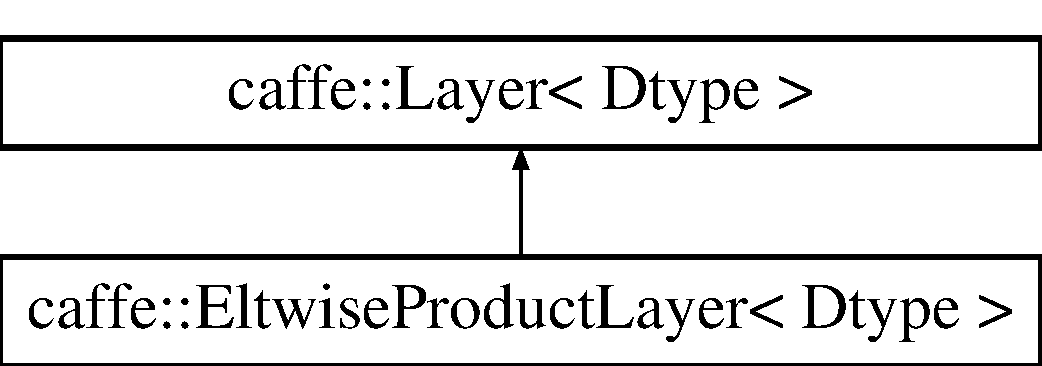
\includegraphics[height=2.000000cm]{classcaffe_1_1_eltwise_product_layer}
\end{center}
\end{figure}
\subsection*{Public Member Functions}
\begin{DoxyCompactItemize}
\item 
\hyperlink{classcaffe_1_1_eltwise_product_layer_ae8ba2b765a0b666927448e5746733044}{Eltwise\+Product\+Layer} (const Layer\+Parameter \&param)
\item 
virtual void \hyperlink{classcaffe_1_1_eltwise_product_layer_ab24fdd7f4a2b47c95fbe80ed1cd5ee08}{Set\+Up} (const vector$<$ \hyperlink{classcaffe_1_1_blob}{Blob}$<$ Dtype $>$ $\ast$ $>$ \&bottom, vector$<$ \hyperlink{classcaffe_1_1_blob}{Blob}$<$ Dtype $>$ $\ast$ $>$ $\ast$top)
\end{DoxyCompactItemize}
\subsection*{Protected Member Functions}
\begin{DoxyCompactItemize}
\item 
virtual Dtype \hyperlink{classcaffe_1_1_eltwise_product_layer_a0c3daabf8f8075f4e94879218941a348}{Forward\+\_\+cpu} (const vector$<$ \hyperlink{classcaffe_1_1_blob}{Blob}$<$ Dtype $>$ $\ast$ $>$ \&bottom, vector$<$ \hyperlink{classcaffe_1_1_blob}{Blob}$<$ Dtype $>$ $\ast$ $>$ $\ast$top)
\item 
virtual Dtype \hyperlink{classcaffe_1_1_eltwise_product_layer_a53cf4aaa04a908dc7ed5ceee48f6054d}{Forward\+\_\+gpu} (const vector$<$ \hyperlink{classcaffe_1_1_blob}{Blob}$<$ Dtype $>$ $\ast$ $>$ \&bottom, vector$<$ \hyperlink{classcaffe_1_1_blob}{Blob}$<$ Dtype $>$ $\ast$ $>$ $\ast$top)
\item 
virtual void \hyperlink{classcaffe_1_1_eltwise_product_layer_a5d03ef5628726c95e71d425137e60d5e}{Backward\+\_\+cpu} (const vector$<$ \hyperlink{classcaffe_1_1_blob}{Blob}$<$ Dtype $>$ $\ast$ $>$ \&top, const bool propagate\+\_\+down, vector$<$ \hyperlink{classcaffe_1_1_blob}{Blob}$<$ Dtype $>$ $\ast$ $>$ $\ast$bottom)
\item 
virtual void \hyperlink{classcaffe_1_1_eltwise_product_layer_a9d5b22fd37b476dd5cab2499c9a69a87}{Backward\+\_\+gpu} (const vector$<$ \hyperlink{classcaffe_1_1_blob}{Blob}$<$ Dtype $>$ $\ast$ $>$ \&top, const bool propagate\+\_\+down, vector$<$ \hyperlink{classcaffe_1_1_blob}{Blob}$<$ Dtype $>$ $\ast$ $>$ $\ast$bottom)
\end{DoxyCompactItemize}
\subsection*{Additional Inherited Members}


\subsection{Constructor \& Destructor Documentation}
\hypertarget{classcaffe_1_1_eltwise_product_layer_ae8ba2b765a0b666927448e5746733044}{\index{caffe\+::\+Eltwise\+Product\+Layer@{caffe\+::\+Eltwise\+Product\+Layer}!Eltwise\+Product\+Layer@{Eltwise\+Product\+Layer}}
\index{Eltwise\+Product\+Layer@{Eltwise\+Product\+Layer}!caffe\+::\+Eltwise\+Product\+Layer@{caffe\+::\+Eltwise\+Product\+Layer}}
\subsubsection[{Eltwise\+Product\+Layer}]{\setlength{\rightskip}{0pt plus 5cm}template$<$typename Dtype $>$ {\bf caffe\+::\+Eltwise\+Product\+Layer}$<$ Dtype $>$\+::{\bf Eltwise\+Product\+Layer} (
\begin{DoxyParamCaption}
\item[{const Layer\+Parameter \&}]{param}
\end{DoxyParamCaption}
)\hspace{0.3cm}{\ttfamily [inline]}, {\ttfamily [explicit]}}}\label{classcaffe_1_1_eltwise_product_layer_ae8ba2b765a0b666927448e5746733044}


\subsection{Member Function Documentation}
\hypertarget{classcaffe_1_1_eltwise_product_layer_a5d03ef5628726c95e71d425137e60d5e}{\index{caffe\+::\+Eltwise\+Product\+Layer@{caffe\+::\+Eltwise\+Product\+Layer}!Backward\+\_\+cpu@{Backward\+\_\+cpu}}
\index{Backward\+\_\+cpu@{Backward\+\_\+cpu}!caffe\+::\+Eltwise\+Product\+Layer@{caffe\+::\+Eltwise\+Product\+Layer}}
\subsubsection[{Backward\+\_\+cpu}]{\setlength{\rightskip}{0pt plus 5cm}template$<$typename Dtype $>$ void {\bf caffe\+::\+Eltwise\+Product\+Layer}$<$ Dtype $>$\+::Backward\+\_\+cpu (
\begin{DoxyParamCaption}
\item[{const vector$<$ {\bf Blob}$<$ Dtype $>$ $\ast$ $>$ \&}]{top, }
\item[{const bool}]{propagate\+\_\+down, }
\item[{vector$<$ {\bf Blob}$<$ Dtype $>$ $\ast$ $>$ $\ast$}]{bottom}
\end{DoxyParamCaption}
)\hspace{0.3cm}{\ttfamily [protected]}, {\ttfamily [virtual]}}}\label{classcaffe_1_1_eltwise_product_layer_a5d03ef5628726c95e71d425137e60d5e}


Implements \hyperlink{classcaffe_1_1_layer_ac2d82011d076237c67997f63e7ee4b80}{caffe\+::\+Layer$<$ Dtype $>$}.

\hypertarget{classcaffe_1_1_eltwise_product_layer_a9d5b22fd37b476dd5cab2499c9a69a87}{\index{caffe\+::\+Eltwise\+Product\+Layer@{caffe\+::\+Eltwise\+Product\+Layer}!Backward\+\_\+gpu@{Backward\+\_\+gpu}}
\index{Backward\+\_\+gpu@{Backward\+\_\+gpu}!caffe\+::\+Eltwise\+Product\+Layer@{caffe\+::\+Eltwise\+Product\+Layer}}
\subsubsection[{Backward\+\_\+gpu}]{\setlength{\rightskip}{0pt plus 5cm}template$<$typename Dtype $>$ void {\bf caffe\+::\+Eltwise\+Product\+Layer}$<$ Dtype $>$\+::Backward\+\_\+gpu (
\begin{DoxyParamCaption}
\item[{const vector$<$ {\bf Blob}$<$ Dtype $>$ $\ast$ $>$ \&}]{top, }
\item[{const bool}]{propagate\+\_\+down, }
\item[{vector$<$ {\bf Blob}$<$ Dtype $>$ $\ast$ $>$ $\ast$}]{bottom}
\end{DoxyParamCaption}
)\hspace{0.3cm}{\ttfamily [protected]}, {\ttfamily [virtual]}}}\label{classcaffe_1_1_eltwise_product_layer_a9d5b22fd37b476dd5cab2499c9a69a87}


Reimplemented from \hyperlink{classcaffe_1_1_layer_adf07ffe1f22d2fd2b1b0ff475ef5a64b}{caffe\+::\+Layer$<$ Dtype $>$}.

\hypertarget{classcaffe_1_1_eltwise_product_layer_a0c3daabf8f8075f4e94879218941a348}{\index{caffe\+::\+Eltwise\+Product\+Layer@{caffe\+::\+Eltwise\+Product\+Layer}!Forward\+\_\+cpu@{Forward\+\_\+cpu}}
\index{Forward\+\_\+cpu@{Forward\+\_\+cpu}!caffe\+::\+Eltwise\+Product\+Layer@{caffe\+::\+Eltwise\+Product\+Layer}}
\subsubsection[{Forward\+\_\+cpu}]{\setlength{\rightskip}{0pt plus 5cm}template$<$typename Dtype $>$ Dtype {\bf caffe\+::\+Eltwise\+Product\+Layer}$<$ Dtype $>$\+::Forward\+\_\+cpu (
\begin{DoxyParamCaption}
\item[{const vector$<$ {\bf Blob}$<$ Dtype $>$ $\ast$ $>$ \&}]{bottom, }
\item[{vector$<$ {\bf Blob}$<$ Dtype $>$ $\ast$ $>$ $\ast$}]{top}
\end{DoxyParamCaption}
)\hspace{0.3cm}{\ttfamily [protected]}, {\ttfamily [virtual]}}}\label{classcaffe_1_1_eltwise_product_layer_a0c3daabf8f8075f4e94879218941a348}


Implements \hyperlink{classcaffe_1_1_layer_a8f7f61da3b8b3ca7f2394dee33873353}{caffe\+::\+Layer$<$ Dtype $>$}.

\hypertarget{classcaffe_1_1_eltwise_product_layer_a53cf4aaa04a908dc7ed5ceee48f6054d}{\index{caffe\+::\+Eltwise\+Product\+Layer@{caffe\+::\+Eltwise\+Product\+Layer}!Forward\+\_\+gpu@{Forward\+\_\+gpu}}
\index{Forward\+\_\+gpu@{Forward\+\_\+gpu}!caffe\+::\+Eltwise\+Product\+Layer@{caffe\+::\+Eltwise\+Product\+Layer}}
\subsubsection[{Forward\+\_\+gpu}]{\setlength{\rightskip}{0pt plus 5cm}template$<$typename Dtype $>$ Dtype {\bf caffe\+::\+Eltwise\+Product\+Layer}$<$ Dtype $>$\+::Forward\+\_\+gpu (
\begin{DoxyParamCaption}
\item[{const vector$<$ {\bf Blob}$<$ Dtype $>$ $\ast$ $>$ \&}]{bottom, }
\item[{vector$<$ {\bf Blob}$<$ Dtype $>$ $\ast$ $>$ $\ast$}]{top}
\end{DoxyParamCaption}
)\hspace{0.3cm}{\ttfamily [protected]}, {\ttfamily [virtual]}}}\label{classcaffe_1_1_eltwise_product_layer_a53cf4aaa04a908dc7ed5ceee48f6054d}


Reimplemented from \hyperlink{classcaffe_1_1_layer_a2d78dbf5d8bc36928bd8f6fcfbafbcef}{caffe\+::\+Layer$<$ Dtype $>$}.

\hypertarget{classcaffe_1_1_eltwise_product_layer_ab24fdd7f4a2b47c95fbe80ed1cd5ee08}{\index{caffe\+::\+Eltwise\+Product\+Layer@{caffe\+::\+Eltwise\+Product\+Layer}!Set\+Up@{Set\+Up}}
\index{Set\+Up@{Set\+Up}!caffe\+::\+Eltwise\+Product\+Layer@{caffe\+::\+Eltwise\+Product\+Layer}}
\subsubsection[{Set\+Up}]{\setlength{\rightskip}{0pt plus 5cm}template$<$typename Dtype $>$ void {\bf caffe\+::\+Eltwise\+Product\+Layer}$<$ Dtype $>$\+::Set\+Up (
\begin{DoxyParamCaption}
\item[{const vector$<$ {\bf Blob}$<$ Dtype $>$ $\ast$ $>$ \&}]{bottom, }
\item[{vector$<$ {\bf Blob}$<$ Dtype $>$ $\ast$ $>$ $\ast$}]{top}
\end{DoxyParamCaption}
)\hspace{0.3cm}{\ttfamily [virtual]}}}\label{classcaffe_1_1_eltwise_product_layer_ab24fdd7f4a2b47c95fbe80ed1cd5ee08}


Implements \hyperlink{classcaffe_1_1_layer_abd13c6489c13953b4fbcfcf6880835d0}{caffe\+::\+Layer$<$ Dtype $>$}.



The documentation for this class was generated from the following files\+:\begin{DoxyCompactItemize}
\item 
include/caffe/\hyperlink{vision__layers_8hpp}{vision\+\_\+layers.\+hpp}\item 
src/caffe/layers/\hyperlink{eltwise__product__layer_8cpp}{eltwise\+\_\+product\+\_\+layer.\+cpp}\item 
src/caffe/layers/\hyperlink{eltwise__product__layer_8cu}{eltwise\+\_\+product\+\_\+layer.\+cu}\end{DoxyCompactItemize}

\hypertarget{classcaffe_1_1_eltwise_product_layer_test}{\section{caffe\+:\+:Eltwise\+Product\+Layer\+Test$<$ Dtype $>$ Class Template Reference}
\label{classcaffe_1_1_eltwise_product_layer_test}\index{caffe\+::\+Eltwise\+Product\+Layer\+Test$<$ Dtype $>$@{caffe\+::\+Eltwise\+Product\+Layer\+Test$<$ Dtype $>$}}
}
Inheritance diagram for caffe\+:\+:Eltwise\+Product\+Layer\+Test$<$ Dtype $>$\+:\begin{figure}[H]
\begin{center}
\leavevmode
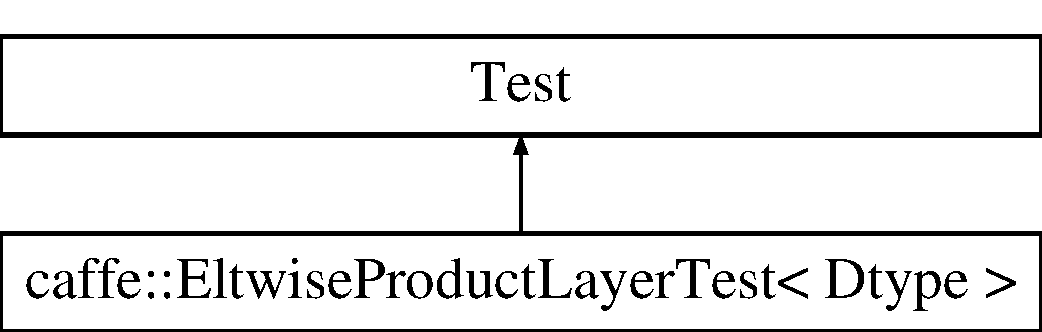
\includegraphics[height=2.000000cm]{classcaffe_1_1_eltwise_product_layer_test}
\end{center}
\end{figure}
\subsection*{Protected Member Functions}
\begin{DoxyCompactItemize}
\item 
\hyperlink{classcaffe_1_1_eltwise_product_layer_test_ad706d4fd901f7a5269258a8ea43c6f43}{Eltwise\+Product\+Layer\+Test} ()
\item 
virtual \hyperlink{classcaffe_1_1_eltwise_product_layer_test_ae3221c2d98478e7ccef5f61d33d971df}{$\sim$\+Eltwise\+Product\+Layer\+Test} ()
\end{DoxyCompactItemize}
\subsection*{Protected Attributes}
\begin{DoxyCompactItemize}
\item 
\hyperlink{classcaffe_1_1_blob}{Blob}$<$ Dtype $>$ $\ast$const \hyperlink{classcaffe_1_1_eltwise_product_layer_test_a99b6a7e85b88545e12bf33ad8d40256c}{blob\+\_\+bottom\+\_\+a\+\_\+}
\item 
\hyperlink{classcaffe_1_1_blob}{Blob}$<$ Dtype $>$ $\ast$const \hyperlink{classcaffe_1_1_eltwise_product_layer_test_a6f22183c4c7ca00ca9d37dd8b044ee33}{blob\+\_\+bottom\+\_\+b\+\_\+}
\item 
\hyperlink{classcaffe_1_1_blob}{Blob}$<$ Dtype $>$ $\ast$const \hyperlink{classcaffe_1_1_eltwise_product_layer_test_ae30c5e2a87e6f87aaca79fa495a5e598}{blob\+\_\+bottom\+\_\+c\+\_\+}
\item 
\hyperlink{classcaffe_1_1_blob}{Blob}$<$ Dtype $>$ $\ast$const \hyperlink{classcaffe_1_1_eltwise_product_layer_test_a3473d2cf8c1b5de2251a98177de1e50e}{blob\+\_\+top\+\_\+}
\item 
vector$<$ \hyperlink{classcaffe_1_1_blob}{Blob}$<$ Dtype $>$ $\ast$ $>$ \hyperlink{classcaffe_1_1_eltwise_product_layer_test_ad32b1991564800fa597cd39b3dd20f92}{blob\+\_\+bottom\+\_\+vec\+\_\+}
\item 
vector$<$ \hyperlink{classcaffe_1_1_blob}{Blob}$<$ Dtype $>$ $\ast$ $>$ \hyperlink{classcaffe_1_1_eltwise_product_layer_test_a59ea3d7e02db32dbfcb14cf068f4ebd8}{blob\+\_\+top\+\_\+vec\+\_\+}
\end{DoxyCompactItemize}


\subsection{Constructor \& Destructor Documentation}
\hypertarget{classcaffe_1_1_eltwise_product_layer_test_ad706d4fd901f7a5269258a8ea43c6f43}{\index{caffe\+::\+Eltwise\+Product\+Layer\+Test@{caffe\+::\+Eltwise\+Product\+Layer\+Test}!Eltwise\+Product\+Layer\+Test@{Eltwise\+Product\+Layer\+Test}}
\index{Eltwise\+Product\+Layer\+Test@{Eltwise\+Product\+Layer\+Test}!caffe\+::\+Eltwise\+Product\+Layer\+Test@{caffe\+::\+Eltwise\+Product\+Layer\+Test}}
\subsubsection[{Eltwise\+Product\+Layer\+Test}]{\setlength{\rightskip}{0pt plus 5cm}template$<$typename Dtype $>$ {\bf caffe\+::\+Eltwise\+Product\+Layer\+Test}$<$ Dtype $>$\+::{\bf Eltwise\+Product\+Layer\+Test} (
\begin{DoxyParamCaption}
{}
\end{DoxyParamCaption}
)\hspace{0.3cm}{\ttfamily [inline]}, {\ttfamily [protected]}}}\label{classcaffe_1_1_eltwise_product_layer_test_ad706d4fd901f7a5269258a8ea43c6f43}
\hypertarget{classcaffe_1_1_eltwise_product_layer_test_ae3221c2d98478e7ccef5f61d33d971df}{\index{caffe\+::\+Eltwise\+Product\+Layer\+Test@{caffe\+::\+Eltwise\+Product\+Layer\+Test}!````~Eltwise\+Product\+Layer\+Test@{$\sim$\+Eltwise\+Product\+Layer\+Test}}
\index{````~Eltwise\+Product\+Layer\+Test@{$\sim$\+Eltwise\+Product\+Layer\+Test}!caffe\+::\+Eltwise\+Product\+Layer\+Test@{caffe\+::\+Eltwise\+Product\+Layer\+Test}}
\subsubsection[{$\sim$\+Eltwise\+Product\+Layer\+Test}]{\setlength{\rightskip}{0pt plus 5cm}template$<$typename Dtype $>$ virtual {\bf caffe\+::\+Eltwise\+Product\+Layer\+Test}$<$ Dtype $>$\+::$\sim${\bf Eltwise\+Product\+Layer\+Test} (
\begin{DoxyParamCaption}
{}
\end{DoxyParamCaption}
)\hspace{0.3cm}{\ttfamily [inline]}, {\ttfamily [protected]}, {\ttfamily [virtual]}}}\label{classcaffe_1_1_eltwise_product_layer_test_ae3221c2d98478e7ccef5f61d33d971df}


\subsection{Member Data Documentation}
\hypertarget{classcaffe_1_1_eltwise_product_layer_test_a99b6a7e85b88545e12bf33ad8d40256c}{\index{caffe\+::\+Eltwise\+Product\+Layer\+Test@{caffe\+::\+Eltwise\+Product\+Layer\+Test}!blob\+\_\+bottom\+\_\+a\+\_\+@{blob\+\_\+bottom\+\_\+a\+\_\+}}
\index{blob\+\_\+bottom\+\_\+a\+\_\+@{blob\+\_\+bottom\+\_\+a\+\_\+}!caffe\+::\+Eltwise\+Product\+Layer\+Test@{caffe\+::\+Eltwise\+Product\+Layer\+Test}}
\subsubsection[{blob\+\_\+bottom\+\_\+a\+\_\+}]{\setlength{\rightskip}{0pt plus 5cm}template$<$typename Dtype $>$ {\bf Blob}$<$Dtype$>$$\ast$ const {\bf caffe\+::\+Eltwise\+Product\+Layer\+Test}$<$ Dtype $>$\+::blob\+\_\+bottom\+\_\+a\+\_\+\hspace{0.3cm}{\ttfamily [protected]}}}\label{classcaffe_1_1_eltwise_product_layer_test_a99b6a7e85b88545e12bf33ad8d40256c}
\hypertarget{classcaffe_1_1_eltwise_product_layer_test_a6f22183c4c7ca00ca9d37dd8b044ee33}{\index{caffe\+::\+Eltwise\+Product\+Layer\+Test@{caffe\+::\+Eltwise\+Product\+Layer\+Test}!blob\+\_\+bottom\+\_\+b\+\_\+@{blob\+\_\+bottom\+\_\+b\+\_\+}}
\index{blob\+\_\+bottom\+\_\+b\+\_\+@{blob\+\_\+bottom\+\_\+b\+\_\+}!caffe\+::\+Eltwise\+Product\+Layer\+Test@{caffe\+::\+Eltwise\+Product\+Layer\+Test}}
\subsubsection[{blob\+\_\+bottom\+\_\+b\+\_\+}]{\setlength{\rightskip}{0pt plus 5cm}template$<$typename Dtype $>$ {\bf Blob}$<$Dtype$>$$\ast$ const {\bf caffe\+::\+Eltwise\+Product\+Layer\+Test}$<$ Dtype $>$\+::blob\+\_\+bottom\+\_\+b\+\_\+\hspace{0.3cm}{\ttfamily [protected]}}}\label{classcaffe_1_1_eltwise_product_layer_test_a6f22183c4c7ca00ca9d37dd8b044ee33}
\hypertarget{classcaffe_1_1_eltwise_product_layer_test_ae30c5e2a87e6f87aaca79fa495a5e598}{\index{caffe\+::\+Eltwise\+Product\+Layer\+Test@{caffe\+::\+Eltwise\+Product\+Layer\+Test}!blob\+\_\+bottom\+\_\+c\+\_\+@{blob\+\_\+bottom\+\_\+c\+\_\+}}
\index{blob\+\_\+bottom\+\_\+c\+\_\+@{blob\+\_\+bottom\+\_\+c\+\_\+}!caffe\+::\+Eltwise\+Product\+Layer\+Test@{caffe\+::\+Eltwise\+Product\+Layer\+Test}}
\subsubsection[{blob\+\_\+bottom\+\_\+c\+\_\+}]{\setlength{\rightskip}{0pt plus 5cm}template$<$typename Dtype $>$ {\bf Blob}$<$Dtype$>$$\ast$ const {\bf caffe\+::\+Eltwise\+Product\+Layer\+Test}$<$ Dtype $>$\+::blob\+\_\+bottom\+\_\+c\+\_\+\hspace{0.3cm}{\ttfamily [protected]}}}\label{classcaffe_1_1_eltwise_product_layer_test_ae30c5e2a87e6f87aaca79fa495a5e598}
\hypertarget{classcaffe_1_1_eltwise_product_layer_test_ad32b1991564800fa597cd39b3dd20f92}{\index{caffe\+::\+Eltwise\+Product\+Layer\+Test@{caffe\+::\+Eltwise\+Product\+Layer\+Test}!blob\+\_\+bottom\+\_\+vec\+\_\+@{blob\+\_\+bottom\+\_\+vec\+\_\+}}
\index{blob\+\_\+bottom\+\_\+vec\+\_\+@{blob\+\_\+bottom\+\_\+vec\+\_\+}!caffe\+::\+Eltwise\+Product\+Layer\+Test@{caffe\+::\+Eltwise\+Product\+Layer\+Test}}
\subsubsection[{blob\+\_\+bottom\+\_\+vec\+\_\+}]{\setlength{\rightskip}{0pt plus 5cm}template$<$typename Dtype $>$ vector$<${\bf Blob}$<$Dtype$>$$\ast$$>$ {\bf caffe\+::\+Eltwise\+Product\+Layer\+Test}$<$ Dtype $>$\+::blob\+\_\+bottom\+\_\+vec\+\_\+\hspace{0.3cm}{\ttfamily [protected]}}}\label{classcaffe_1_1_eltwise_product_layer_test_ad32b1991564800fa597cd39b3dd20f92}
\hypertarget{classcaffe_1_1_eltwise_product_layer_test_a3473d2cf8c1b5de2251a98177de1e50e}{\index{caffe\+::\+Eltwise\+Product\+Layer\+Test@{caffe\+::\+Eltwise\+Product\+Layer\+Test}!blob\+\_\+top\+\_\+@{blob\+\_\+top\+\_\+}}
\index{blob\+\_\+top\+\_\+@{blob\+\_\+top\+\_\+}!caffe\+::\+Eltwise\+Product\+Layer\+Test@{caffe\+::\+Eltwise\+Product\+Layer\+Test}}
\subsubsection[{blob\+\_\+top\+\_\+}]{\setlength{\rightskip}{0pt plus 5cm}template$<$typename Dtype $>$ {\bf Blob}$<$Dtype$>$$\ast$ const {\bf caffe\+::\+Eltwise\+Product\+Layer\+Test}$<$ Dtype $>$\+::blob\+\_\+top\+\_\+\hspace{0.3cm}{\ttfamily [protected]}}}\label{classcaffe_1_1_eltwise_product_layer_test_a3473d2cf8c1b5de2251a98177de1e50e}
\hypertarget{classcaffe_1_1_eltwise_product_layer_test_a59ea3d7e02db32dbfcb14cf068f4ebd8}{\index{caffe\+::\+Eltwise\+Product\+Layer\+Test@{caffe\+::\+Eltwise\+Product\+Layer\+Test}!blob\+\_\+top\+\_\+vec\+\_\+@{blob\+\_\+top\+\_\+vec\+\_\+}}
\index{blob\+\_\+top\+\_\+vec\+\_\+@{blob\+\_\+top\+\_\+vec\+\_\+}!caffe\+::\+Eltwise\+Product\+Layer\+Test@{caffe\+::\+Eltwise\+Product\+Layer\+Test}}
\subsubsection[{blob\+\_\+top\+\_\+vec\+\_\+}]{\setlength{\rightskip}{0pt plus 5cm}template$<$typename Dtype $>$ vector$<${\bf Blob}$<$Dtype$>$$\ast$$>$ {\bf caffe\+::\+Eltwise\+Product\+Layer\+Test}$<$ Dtype $>$\+::blob\+\_\+top\+\_\+vec\+\_\+\hspace{0.3cm}{\ttfamily [protected]}}}\label{classcaffe_1_1_eltwise_product_layer_test_a59ea3d7e02db32dbfcb14cf068f4ebd8}


The documentation for this class was generated from the following file\+:\begin{DoxyCompactItemize}
\item 
src/caffe/test/\hyperlink{test__eltwise__product__layer_8cpp}{test\+\_\+eltwise\+\_\+product\+\_\+layer.\+cpp}\end{DoxyCompactItemize}

\hypertarget{classcaffe_1_1_euclidean_loss_layer}{\section{caffe\+:\+:Euclidean\+Loss\+Layer$<$ Dtype $>$ Class Template Reference}
\label{classcaffe_1_1_euclidean_loss_layer}\index{caffe\+::\+Euclidean\+Loss\+Layer$<$ Dtype $>$@{caffe\+::\+Euclidean\+Loss\+Layer$<$ Dtype $>$}}
}


{\ttfamily \#include $<$vision\+\_\+layers.\+hpp$>$}

Inheritance diagram for caffe\+:\+:Euclidean\+Loss\+Layer$<$ Dtype $>$\+:\begin{figure}[H]
\begin{center}
\leavevmode
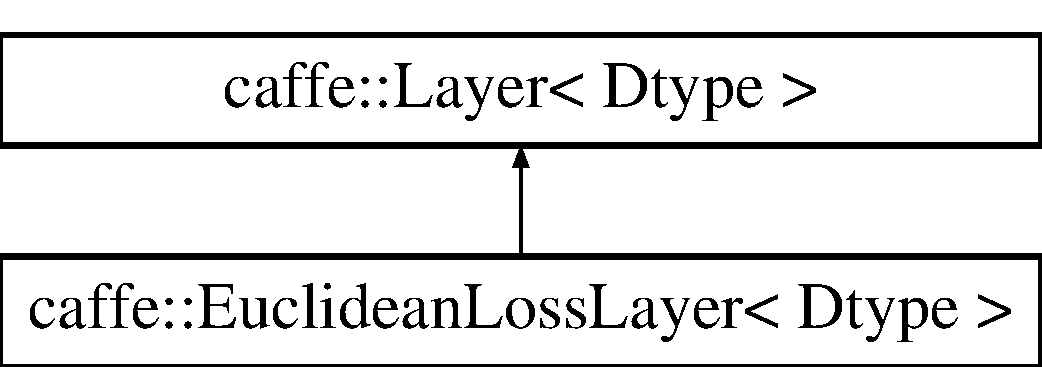
\includegraphics[height=2.000000cm]{classcaffe_1_1_euclidean_loss_layer}
\end{center}
\end{figure}
\subsection*{Public Member Functions}
\begin{DoxyCompactItemize}
\item 
\hyperlink{classcaffe_1_1_euclidean_loss_layer_aea3a6d5454ee1a0db7cdb6c59bcfc5c8}{Euclidean\+Loss\+Layer} (const Layer\+Parameter \&param)
\item 
virtual void \hyperlink{classcaffe_1_1_euclidean_loss_layer_a636a0ded0ca547c4af9b150953bce124}{Set\+Up} (const vector$<$ \hyperlink{classcaffe_1_1_blob}{Blob}$<$ Dtype $>$ $\ast$ $>$ \&bottom, vector$<$ \hyperlink{classcaffe_1_1_blob}{Blob}$<$ Dtype $>$ $\ast$ $>$ $\ast$top)
\end{DoxyCompactItemize}
\subsection*{Protected Member Functions}
\begin{DoxyCompactItemize}
\item 
virtual Dtype \hyperlink{classcaffe_1_1_euclidean_loss_layer_ab3b17e7f7064f68b253df8d463f44dfc}{Forward\+\_\+cpu} (const vector$<$ \hyperlink{classcaffe_1_1_blob}{Blob}$<$ Dtype $>$ $\ast$ $>$ \&bottom, vector$<$ \hyperlink{classcaffe_1_1_blob}{Blob}$<$ Dtype $>$ $\ast$ $>$ $\ast$top)
\item 
virtual void \hyperlink{classcaffe_1_1_euclidean_loss_layer_aeca6594a25c462a4764f6c2e07224b2d}{Backward\+\_\+cpu} (const vector$<$ \hyperlink{classcaffe_1_1_blob}{Blob}$<$ Dtype $>$ $\ast$ $>$ \&top, const bool propagate\+\_\+down, vector$<$ \hyperlink{classcaffe_1_1_blob}{Blob}$<$ Dtype $>$ $\ast$ $>$ $\ast$bottom)
\end{DoxyCompactItemize}
\subsection*{Protected Attributes}
\begin{DoxyCompactItemize}
\item 
\hyperlink{classcaffe_1_1_blob}{Blob}$<$ Dtype $>$ \hyperlink{classcaffe_1_1_euclidean_loss_layer_ad0cfd53b6ffc884b62f237bc0b2b447e}{difference\+\_\+}
\end{DoxyCompactItemize}


\subsection{Constructor \& Destructor Documentation}
\hypertarget{classcaffe_1_1_euclidean_loss_layer_aea3a6d5454ee1a0db7cdb6c59bcfc5c8}{\index{caffe\+::\+Euclidean\+Loss\+Layer@{caffe\+::\+Euclidean\+Loss\+Layer}!Euclidean\+Loss\+Layer@{Euclidean\+Loss\+Layer}}
\index{Euclidean\+Loss\+Layer@{Euclidean\+Loss\+Layer}!caffe\+::\+Euclidean\+Loss\+Layer@{caffe\+::\+Euclidean\+Loss\+Layer}}
\subsubsection[{Euclidean\+Loss\+Layer}]{\setlength{\rightskip}{0pt plus 5cm}template$<$typename Dtype $>$ {\bf caffe\+::\+Euclidean\+Loss\+Layer}$<$ Dtype $>$\+::{\bf Euclidean\+Loss\+Layer} (
\begin{DoxyParamCaption}
\item[{const Layer\+Parameter \&}]{param}
\end{DoxyParamCaption}
)\hspace{0.3cm}{\ttfamily [inline]}, {\ttfamily [explicit]}}}\label{classcaffe_1_1_euclidean_loss_layer_aea3a6d5454ee1a0db7cdb6c59bcfc5c8}


\subsection{Member Function Documentation}
\hypertarget{classcaffe_1_1_euclidean_loss_layer_aeca6594a25c462a4764f6c2e07224b2d}{\index{caffe\+::\+Euclidean\+Loss\+Layer@{caffe\+::\+Euclidean\+Loss\+Layer}!Backward\+\_\+cpu@{Backward\+\_\+cpu}}
\index{Backward\+\_\+cpu@{Backward\+\_\+cpu}!caffe\+::\+Euclidean\+Loss\+Layer@{caffe\+::\+Euclidean\+Loss\+Layer}}
\subsubsection[{Backward\+\_\+cpu}]{\setlength{\rightskip}{0pt plus 5cm}template$<$typename Dtype $>$ void {\bf caffe\+::\+Euclidean\+Loss\+Layer}$<$ Dtype $>$\+::Backward\+\_\+cpu (
\begin{DoxyParamCaption}
\item[{const vector$<$ {\bf Blob}$<$ Dtype $>$ $\ast$ $>$ \&}]{top, }
\item[{const bool}]{propagate\+\_\+down, }
\item[{vector$<$ {\bf Blob}$<$ Dtype $>$ $\ast$ $>$ $\ast$}]{bottom}
\end{DoxyParamCaption}
)\hspace{0.3cm}{\ttfamily [protected]}, {\ttfamily [virtual]}}}\label{classcaffe_1_1_euclidean_loss_layer_aeca6594a25c462a4764f6c2e07224b2d}


Implements \hyperlink{classcaffe_1_1_layer_ac2d82011d076237c67997f63e7ee4b80}{caffe\+::\+Layer$<$ Dtype $>$}.

\hypertarget{classcaffe_1_1_euclidean_loss_layer_ab3b17e7f7064f68b253df8d463f44dfc}{\index{caffe\+::\+Euclidean\+Loss\+Layer@{caffe\+::\+Euclidean\+Loss\+Layer}!Forward\+\_\+cpu@{Forward\+\_\+cpu}}
\index{Forward\+\_\+cpu@{Forward\+\_\+cpu}!caffe\+::\+Euclidean\+Loss\+Layer@{caffe\+::\+Euclidean\+Loss\+Layer}}
\subsubsection[{Forward\+\_\+cpu}]{\setlength{\rightskip}{0pt plus 5cm}template$<$typename Dtype $>$ Dtype {\bf caffe\+::\+Euclidean\+Loss\+Layer}$<$ Dtype $>$\+::Forward\+\_\+cpu (
\begin{DoxyParamCaption}
\item[{const vector$<$ {\bf Blob}$<$ Dtype $>$ $\ast$ $>$ \&}]{bottom, }
\item[{vector$<$ {\bf Blob}$<$ Dtype $>$ $\ast$ $>$ $\ast$}]{top}
\end{DoxyParamCaption}
)\hspace{0.3cm}{\ttfamily [protected]}, {\ttfamily [virtual]}}}\label{classcaffe_1_1_euclidean_loss_layer_ab3b17e7f7064f68b253df8d463f44dfc}


Implements \hyperlink{classcaffe_1_1_layer_a8f7f61da3b8b3ca7f2394dee33873353}{caffe\+::\+Layer$<$ Dtype $>$}.

\hypertarget{classcaffe_1_1_euclidean_loss_layer_a636a0ded0ca547c4af9b150953bce124}{\index{caffe\+::\+Euclidean\+Loss\+Layer@{caffe\+::\+Euclidean\+Loss\+Layer}!Set\+Up@{Set\+Up}}
\index{Set\+Up@{Set\+Up}!caffe\+::\+Euclidean\+Loss\+Layer@{caffe\+::\+Euclidean\+Loss\+Layer}}
\subsubsection[{Set\+Up}]{\setlength{\rightskip}{0pt plus 5cm}template$<$typename Dtype $>$ void {\bf caffe\+::\+Euclidean\+Loss\+Layer}$<$ Dtype $>$\+::Set\+Up (
\begin{DoxyParamCaption}
\item[{const vector$<$ {\bf Blob}$<$ Dtype $>$ $\ast$ $>$ \&}]{bottom, }
\item[{vector$<$ {\bf Blob}$<$ Dtype $>$ $\ast$ $>$ $\ast$}]{top}
\end{DoxyParamCaption}
)\hspace{0.3cm}{\ttfamily [virtual]}}}\label{classcaffe_1_1_euclidean_loss_layer_a636a0ded0ca547c4af9b150953bce124}


Implements \hyperlink{classcaffe_1_1_layer_abd13c6489c13953b4fbcfcf6880835d0}{caffe\+::\+Layer$<$ Dtype $>$}.



\subsection{Member Data Documentation}
\hypertarget{classcaffe_1_1_euclidean_loss_layer_ad0cfd53b6ffc884b62f237bc0b2b447e}{\index{caffe\+::\+Euclidean\+Loss\+Layer@{caffe\+::\+Euclidean\+Loss\+Layer}!difference\+\_\+@{difference\+\_\+}}
\index{difference\+\_\+@{difference\+\_\+}!caffe\+::\+Euclidean\+Loss\+Layer@{caffe\+::\+Euclidean\+Loss\+Layer}}
\subsubsection[{difference\+\_\+}]{\setlength{\rightskip}{0pt plus 5cm}template$<$typename Dtype $>$ {\bf Blob}$<$Dtype$>$ {\bf caffe\+::\+Euclidean\+Loss\+Layer}$<$ Dtype $>$\+::difference\+\_\+\hspace{0.3cm}{\ttfamily [protected]}}}\label{classcaffe_1_1_euclidean_loss_layer_ad0cfd53b6ffc884b62f237bc0b2b447e}


The documentation for this class was generated from the following files\+:\begin{DoxyCompactItemize}
\item 
include/caffe/\hyperlink{vision__layers_8hpp}{vision\+\_\+layers.\+hpp}\item 
src/caffe/layers/\hyperlink{loss__layer_8cpp}{loss\+\_\+layer.\+cpp}\end{DoxyCompactItemize}

\hypertarget{classcaffe_1_1_euclidean_loss_layer_test}{\section{caffe\+:\+:Euclidean\+Loss\+Layer\+Test$<$ Dtype $>$ Class Template Reference}
\label{classcaffe_1_1_euclidean_loss_layer_test}\index{caffe\+::\+Euclidean\+Loss\+Layer\+Test$<$ Dtype $>$@{caffe\+::\+Euclidean\+Loss\+Layer\+Test$<$ Dtype $>$}}
}
Inheritance diagram for caffe\+:\+:Euclidean\+Loss\+Layer\+Test$<$ Dtype $>$\+:\begin{figure}[H]
\begin{center}
\leavevmode
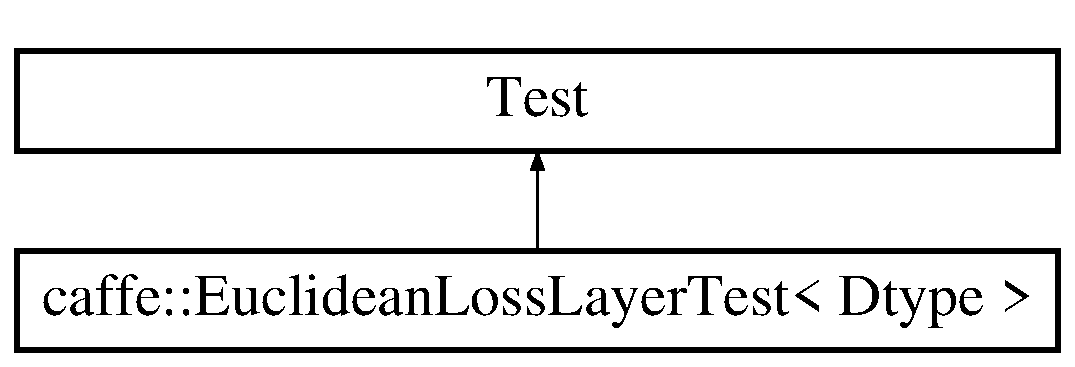
\includegraphics[height=2.000000cm]{classcaffe_1_1_euclidean_loss_layer_test}
\end{center}
\end{figure}
\subsection*{Protected Member Functions}
\begin{DoxyCompactItemize}
\item 
\hyperlink{classcaffe_1_1_euclidean_loss_layer_test_a40a2a4d9ec95bba4b2bbd65a02f2784a}{Euclidean\+Loss\+Layer\+Test} ()
\item 
virtual \hyperlink{classcaffe_1_1_euclidean_loss_layer_test_aec948651fe388f06646ad36e57a85317}{$\sim$\+Euclidean\+Loss\+Layer\+Test} ()
\end{DoxyCompactItemize}
\subsection*{Protected Attributes}
\begin{DoxyCompactItemize}
\item 
\hyperlink{classcaffe_1_1_blob}{Blob}$<$ Dtype $>$ $\ast$const \hyperlink{classcaffe_1_1_euclidean_loss_layer_test_aa502435549ee6a7597a60f66aaecc4ea}{blob\+\_\+bottom\+\_\+data\+\_\+}
\item 
\hyperlink{classcaffe_1_1_blob}{Blob}$<$ Dtype $>$ $\ast$const \hyperlink{classcaffe_1_1_euclidean_loss_layer_test_ae2509956f3d64e647a9e704c428189ae}{blob\+\_\+bottom\+\_\+label\+\_\+}
\item 
vector$<$ \hyperlink{classcaffe_1_1_blob}{Blob}$<$ Dtype $>$ $\ast$ $>$ \hyperlink{classcaffe_1_1_euclidean_loss_layer_test_ace037a9615b21b31c469aee9fcdf76ae}{blob\+\_\+bottom\+\_\+vec\+\_\+}
\item 
vector$<$ \hyperlink{classcaffe_1_1_blob}{Blob}$<$ Dtype $>$ $\ast$ $>$ \hyperlink{classcaffe_1_1_euclidean_loss_layer_test_a0613ceccb5843e4c6880d4f348d73519}{blob\+\_\+top\+\_\+vec\+\_\+}
\end{DoxyCompactItemize}


\subsection{Constructor \& Destructor Documentation}
\hypertarget{classcaffe_1_1_euclidean_loss_layer_test_a40a2a4d9ec95bba4b2bbd65a02f2784a}{\index{caffe\+::\+Euclidean\+Loss\+Layer\+Test@{caffe\+::\+Euclidean\+Loss\+Layer\+Test}!Euclidean\+Loss\+Layer\+Test@{Euclidean\+Loss\+Layer\+Test}}
\index{Euclidean\+Loss\+Layer\+Test@{Euclidean\+Loss\+Layer\+Test}!caffe\+::\+Euclidean\+Loss\+Layer\+Test@{caffe\+::\+Euclidean\+Loss\+Layer\+Test}}
\subsubsection[{Euclidean\+Loss\+Layer\+Test}]{\setlength{\rightskip}{0pt plus 5cm}template$<$typename Dtype $>$ {\bf caffe\+::\+Euclidean\+Loss\+Layer\+Test}$<$ Dtype $>$\+::{\bf Euclidean\+Loss\+Layer\+Test} (
\begin{DoxyParamCaption}
{}
\end{DoxyParamCaption}
)\hspace{0.3cm}{\ttfamily [inline]}, {\ttfamily [protected]}}}\label{classcaffe_1_1_euclidean_loss_layer_test_a40a2a4d9ec95bba4b2bbd65a02f2784a}
\hypertarget{classcaffe_1_1_euclidean_loss_layer_test_aec948651fe388f06646ad36e57a85317}{\index{caffe\+::\+Euclidean\+Loss\+Layer\+Test@{caffe\+::\+Euclidean\+Loss\+Layer\+Test}!````~Euclidean\+Loss\+Layer\+Test@{$\sim$\+Euclidean\+Loss\+Layer\+Test}}
\index{````~Euclidean\+Loss\+Layer\+Test@{$\sim$\+Euclidean\+Loss\+Layer\+Test}!caffe\+::\+Euclidean\+Loss\+Layer\+Test@{caffe\+::\+Euclidean\+Loss\+Layer\+Test}}
\subsubsection[{$\sim$\+Euclidean\+Loss\+Layer\+Test}]{\setlength{\rightskip}{0pt plus 5cm}template$<$typename Dtype $>$ virtual {\bf caffe\+::\+Euclidean\+Loss\+Layer\+Test}$<$ Dtype $>$\+::$\sim${\bf Euclidean\+Loss\+Layer\+Test} (
\begin{DoxyParamCaption}
{}
\end{DoxyParamCaption}
)\hspace{0.3cm}{\ttfamily [inline]}, {\ttfamily [protected]}, {\ttfamily [virtual]}}}\label{classcaffe_1_1_euclidean_loss_layer_test_aec948651fe388f06646ad36e57a85317}


\subsection{Member Data Documentation}
\hypertarget{classcaffe_1_1_euclidean_loss_layer_test_aa502435549ee6a7597a60f66aaecc4ea}{\index{caffe\+::\+Euclidean\+Loss\+Layer\+Test@{caffe\+::\+Euclidean\+Loss\+Layer\+Test}!blob\+\_\+bottom\+\_\+data\+\_\+@{blob\+\_\+bottom\+\_\+data\+\_\+}}
\index{blob\+\_\+bottom\+\_\+data\+\_\+@{blob\+\_\+bottom\+\_\+data\+\_\+}!caffe\+::\+Euclidean\+Loss\+Layer\+Test@{caffe\+::\+Euclidean\+Loss\+Layer\+Test}}
\subsubsection[{blob\+\_\+bottom\+\_\+data\+\_\+}]{\setlength{\rightskip}{0pt plus 5cm}template$<$typename Dtype $>$ {\bf Blob}$<$Dtype$>$$\ast$ const {\bf caffe\+::\+Euclidean\+Loss\+Layer\+Test}$<$ Dtype $>$\+::blob\+\_\+bottom\+\_\+data\+\_\+\hspace{0.3cm}{\ttfamily [protected]}}}\label{classcaffe_1_1_euclidean_loss_layer_test_aa502435549ee6a7597a60f66aaecc4ea}
\hypertarget{classcaffe_1_1_euclidean_loss_layer_test_ae2509956f3d64e647a9e704c428189ae}{\index{caffe\+::\+Euclidean\+Loss\+Layer\+Test@{caffe\+::\+Euclidean\+Loss\+Layer\+Test}!blob\+\_\+bottom\+\_\+label\+\_\+@{blob\+\_\+bottom\+\_\+label\+\_\+}}
\index{blob\+\_\+bottom\+\_\+label\+\_\+@{blob\+\_\+bottom\+\_\+label\+\_\+}!caffe\+::\+Euclidean\+Loss\+Layer\+Test@{caffe\+::\+Euclidean\+Loss\+Layer\+Test}}
\subsubsection[{blob\+\_\+bottom\+\_\+label\+\_\+}]{\setlength{\rightskip}{0pt plus 5cm}template$<$typename Dtype $>$ {\bf Blob}$<$Dtype$>$$\ast$ const {\bf caffe\+::\+Euclidean\+Loss\+Layer\+Test}$<$ Dtype $>$\+::blob\+\_\+bottom\+\_\+label\+\_\+\hspace{0.3cm}{\ttfamily [protected]}}}\label{classcaffe_1_1_euclidean_loss_layer_test_ae2509956f3d64e647a9e704c428189ae}
\hypertarget{classcaffe_1_1_euclidean_loss_layer_test_ace037a9615b21b31c469aee9fcdf76ae}{\index{caffe\+::\+Euclidean\+Loss\+Layer\+Test@{caffe\+::\+Euclidean\+Loss\+Layer\+Test}!blob\+\_\+bottom\+\_\+vec\+\_\+@{blob\+\_\+bottom\+\_\+vec\+\_\+}}
\index{blob\+\_\+bottom\+\_\+vec\+\_\+@{blob\+\_\+bottom\+\_\+vec\+\_\+}!caffe\+::\+Euclidean\+Loss\+Layer\+Test@{caffe\+::\+Euclidean\+Loss\+Layer\+Test}}
\subsubsection[{blob\+\_\+bottom\+\_\+vec\+\_\+}]{\setlength{\rightskip}{0pt plus 5cm}template$<$typename Dtype $>$ vector$<${\bf Blob}$<$Dtype$>$$\ast$$>$ {\bf caffe\+::\+Euclidean\+Loss\+Layer\+Test}$<$ Dtype $>$\+::blob\+\_\+bottom\+\_\+vec\+\_\+\hspace{0.3cm}{\ttfamily [protected]}}}\label{classcaffe_1_1_euclidean_loss_layer_test_ace037a9615b21b31c469aee9fcdf76ae}
\hypertarget{classcaffe_1_1_euclidean_loss_layer_test_a0613ceccb5843e4c6880d4f348d73519}{\index{caffe\+::\+Euclidean\+Loss\+Layer\+Test@{caffe\+::\+Euclidean\+Loss\+Layer\+Test}!blob\+\_\+top\+\_\+vec\+\_\+@{blob\+\_\+top\+\_\+vec\+\_\+}}
\index{blob\+\_\+top\+\_\+vec\+\_\+@{blob\+\_\+top\+\_\+vec\+\_\+}!caffe\+::\+Euclidean\+Loss\+Layer\+Test@{caffe\+::\+Euclidean\+Loss\+Layer\+Test}}
\subsubsection[{blob\+\_\+top\+\_\+vec\+\_\+}]{\setlength{\rightskip}{0pt plus 5cm}template$<$typename Dtype $>$ vector$<${\bf Blob}$<$Dtype$>$$\ast$$>$ {\bf caffe\+::\+Euclidean\+Loss\+Layer\+Test}$<$ Dtype $>$\+::blob\+\_\+top\+\_\+vec\+\_\+\hspace{0.3cm}{\ttfamily [protected]}}}\label{classcaffe_1_1_euclidean_loss_layer_test_a0613ceccb5843e4c6880d4f348d73519}


The documentation for this class was generated from the following file\+:\begin{DoxyCompactItemize}
\item 
src/caffe/test/\hyperlink{test__euclidean__loss__layer_8cpp}{test\+\_\+euclidean\+\_\+loss\+\_\+layer.\+cpp}\end{DoxyCompactItemize}

\hypertarget{classcaffe_1_1_filler}{\section{caffe\+:\+:Filler$<$ Dtype $>$ Class Template Reference}
\label{classcaffe_1_1_filler}\index{caffe\+::\+Filler$<$ Dtype $>$@{caffe\+::\+Filler$<$ Dtype $>$}}
}


{\ttfamily \#include $<$filler.\+hpp$>$}

Inheritance diagram for caffe\+:\+:Filler$<$ Dtype $>$\+:\begin{figure}[H]
\begin{center}
\leavevmode
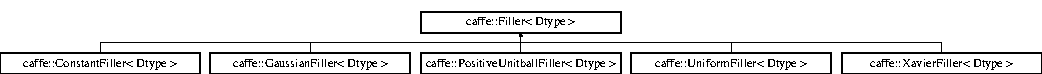
\includegraphics[height=0.991150cm]{classcaffe_1_1_filler}
\end{center}
\end{figure}
\subsection*{Public Member Functions}
\begin{DoxyCompactItemize}
\item 
\hyperlink{classcaffe_1_1_filler_aff156b1d4e5dbbbad720aa776df44512}{Filler} (const Filler\+Parameter \&param)
\item 
virtual \hyperlink{classcaffe_1_1_filler_af24dcc49f4309797a2c0ee830f111dc7}{$\sim$\+Filler} ()
\item 
virtual void \hyperlink{classcaffe_1_1_filler_acd02177b669381252a7c484f51432d30}{Fill} (\hyperlink{classcaffe_1_1_blob}{Blob}$<$ Dtype $>$ $\ast$blob)=0
\end{DoxyCompactItemize}
\subsection*{Protected Attributes}
\begin{DoxyCompactItemize}
\item 
Filler\+Parameter \hyperlink{classcaffe_1_1_filler_a1ded14cf43eeb7b45628770842c4348c}{filler\+\_\+param\+\_\+}
\end{DoxyCompactItemize}


\subsection{Constructor \& Destructor Documentation}
\hypertarget{classcaffe_1_1_filler_aff156b1d4e5dbbbad720aa776df44512}{\index{caffe\+::\+Filler@{caffe\+::\+Filler}!Filler@{Filler}}
\index{Filler@{Filler}!caffe\+::\+Filler@{caffe\+::\+Filler}}
\subsubsection[{Filler}]{\setlength{\rightskip}{0pt plus 5cm}template$<$typename Dtype $>$ {\bf caffe\+::\+Filler}$<$ Dtype $>$\+::{\bf Filler} (
\begin{DoxyParamCaption}
\item[{const Filler\+Parameter \&}]{param}
\end{DoxyParamCaption}
)\hspace{0.3cm}{\ttfamily [inline]}, {\ttfamily [explicit]}}}\label{classcaffe_1_1_filler_aff156b1d4e5dbbbad720aa776df44512}
\hypertarget{classcaffe_1_1_filler_af24dcc49f4309797a2c0ee830f111dc7}{\index{caffe\+::\+Filler@{caffe\+::\+Filler}!````~Filler@{$\sim$\+Filler}}
\index{````~Filler@{$\sim$\+Filler}!caffe\+::\+Filler@{caffe\+::\+Filler}}
\subsubsection[{$\sim$\+Filler}]{\setlength{\rightskip}{0pt plus 5cm}template$<$typename Dtype $>$ virtual {\bf caffe\+::\+Filler}$<$ Dtype $>$\+::$\sim${\bf Filler} (
\begin{DoxyParamCaption}
{}
\end{DoxyParamCaption}
)\hspace{0.3cm}{\ttfamily [inline]}, {\ttfamily [virtual]}}}\label{classcaffe_1_1_filler_af24dcc49f4309797a2c0ee830f111dc7}


\subsection{Member Function Documentation}
\hypertarget{classcaffe_1_1_filler_acd02177b669381252a7c484f51432d30}{\index{caffe\+::\+Filler@{caffe\+::\+Filler}!Fill@{Fill}}
\index{Fill@{Fill}!caffe\+::\+Filler@{caffe\+::\+Filler}}
\subsubsection[{Fill}]{\setlength{\rightskip}{0pt plus 5cm}template$<$typename Dtype $>$ virtual void {\bf caffe\+::\+Filler}$<$ Dtype $>$\+::Fill (
\begin{DoxyParamCaption}
\item[{{\bf Blob}$<$ Dtype $>$ $\ast$}]{blob}
\end{DoxyParamCaption}
)\hspace{0.3cm}{\ttfamily [pure virtual]}}}\label{classcaffe_1_1_filler_acd02177b669381252a7c484f51432d30}


Implemented in \hyperlink{classcaffe_1_1_xavier_filler_af61c37b2a24ebc70c9e7d2d3d703d2c8}{caffe\+::\+Xavier\+Filler$<$ Dtype $>$}, \hyperlink{classcaffe_1_1_positive_unitball_filler_a8ace4f586a5aa3eab7de1dd796556f42}{caffe\+::\+Positive\+Unitball\+Filler$<$ Dtype $>$}, \hyperlink{classcaffe_1_1_gaussian_filler_ac45d5d0695521d7d71a4d5bccb659f21}{caffe\+::\+Gaussian\+Filler$<$ Dtype $>$}, \hyperlink{classcaffe_1_1_uniform_filler_ae874946013d1b9ec4ede19786da34a9d}{caffe\+::\+Uniform\+Filler$<$ Dtype $>$}, and \hyperlink{classcaffe_1_1_constant_filler_a411cf44b177109c388c0b34c906f4e8e}{caffe\+::\+Constant\+Filler$<$ Dtype $>$}.



\subsection{Member Data Documentation}
\hypertarget{classcaffe_1_1_filler_a1ded14cf43eeb7b45628770842c4348c}{\index{caffe\+::\+Filler@{caffe\+::\+Filler}!filler\+\_\+param\+\_\+@{filler\+\_\+param\+\_\+}}
\index{filler\+\_\+param\+\_\+@{filler\+\_\+param\+\_\+}!caffe\+::\+Filler@{caffe\+::\+Filler}}
\subsubsection[{filler\+\_\+param\+\_\+}]{\setlength{\rightskip}{0pt plus 5cm}template$<$typename Dtype $>$ Filler\+Parameter {\bf caffe\+::\+Filler}$<$ Dtype $>$\+::filler\+\_\+param\+\_\+\hspace{0.3cm}{\ttfamily [protected]}}}\label{classcaffe_1_1_filler_a1ded14cf43eeb7b45628770842c4348c}


The documentation for this class was generated from the following file\+:\begin{DoxyCompactItemize}
\item 
include/caffe/\hyperlink{filler_8hpp}{filler.\+hpp}\end{DoxyCompactItemize}

\hypertarget{classcaffe_1_1_flatten_layer}{\section{caffe\+:\+:Flatten\+Layer$<$ Dtype $>$ Class Template Reference}
\label{classcaffe_1_1_flatten_layer}\index{caffe\+::\+Flatten\+Layer$<$ Dtype $>$@{caffe\+::\+Flatten\+Layer$<$ Dtype $>$}}
}


{\ttfamily \#include $<$vision\+\_\+layers.\+hpp$>$}

Inheritance diagram for caffe\+:\+:Flatten\+Layer$<$ Dtype $>$\+:\begin{figure}[H]
\begin{center}
\leavevmode
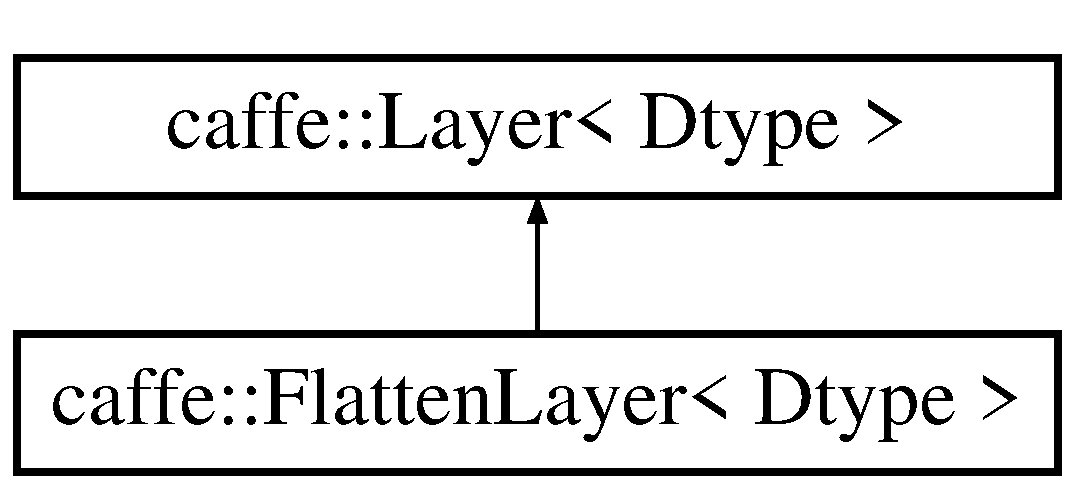
\includegraphics[height=2.000000cm]{classcaffe_1_1_flatten_layer}
\end{center}
\end{figure}
\subsection*{Public Member Functions}
\begin{DoxyCompactItemize}
\item 
\hyperlink{classcaffe_1_1_flatten_layer_a7ab62567c2fb5424979dc16af273b688}{Flatten\+Layer} (const Layer\+Parameter \&param)
\item 
virtual void \hyperlink{classcaffe_1_1_flatten_layer_a49568781c51bfd9e762007910127254e}{Set\+Up} (const vector$<$ \hyperlink{classcaffe_1_1_blob}{Blob}$<$ Dtype $>$ $\ast$ $>$ \&bottom, vector$<$ \hyperlink{classcaffe_1_1_blob}{Blob}$<$ Dtype $>$ $\ast$ $>$ $\ast$top)
\end{DoxyCompactItemize}
\subsection*{Protected Member Functions}
\begin{DoxyCompactItemize}
\item 
virtual Dtype \hyperlink{classcaffe_1_1_flatten_layer_a53caee1cc9658db97e9daefbcdffdc12}{Forward\+\_\+cpu} (const vector$<$ \hyperlink{classcaffe_1_1_blob}{Blob}$<$ Dtype $>$ $\ast$ $>$ \&bottom, vector$<$ \hyperlink{classcaffe_1_1_blob}{Blob}$<$ Dtype $>$ $\ast$ $>$ $\ast$top)
\item 
virtual Dtype \hyperlink{classcaffe_1_1_flatten_layer_a30c8f30255ed20ef7351673aacdbe680}{Forward\+\_\+gpu} (const vector$<$ \hyperlink{classcaffe_1_1_blob}{Blob}$<$ Dtype $>$ $\ast$ $>$ \&bottom, vector$<$ \hyperlink{classcaffe_1_1_blob}{Blob}$<$ Dtype $>$ $\ast$ $>$ $\ast$top)
\item 
virtual void \hyperlink{classcaffe_1_1_flatten_layer_a5b7439a850684ebd8901180853809a50}{Backward\+\_\+cpu} (const vector$<$ \hyperlink{classcaffe_1_1_blob}{Blob}$<$ Dtype $>$ $\ast$ $>$ \&top, const bool propagate\+\_\+down, vector$<$ \hyperlink{classcaffe_1_1_blob}{Blob}$<$ Dtype $>$ $\ast$ $>$ $\ast$bottom)
\item 
virtual void \hyperlink{classcaffe_1_1_flatten_layer_ae5f1044beb9b5c4d60ff8fd5487ad338}{Backward\+\_\+gpu} (const vector$<$ \hyperlink{classcaffe_1_1_blob}{Blob}$<$ Dtype $>$ $\ast$ $>$ \&top, const bool propagate\+\_\+down, vector$<$ \hyperlink{classcaffe_1_1_blob}{Blob}$<$ Dtype $>$ $\ast$ $>$ $\ast$bottom)
\end{DoxyCompactItemize}
\subsection*{Protected Attributes}
\begin{DoxyCompactItemize}
\item 
int \hyperlink{classcaffe_1_1_flatten_layer_ac162173144262f64a0450799072d4090}{count\+\_\+}
\end{DoxyCompactItemize}


\subsection{Constructor \& Destructor Documentation}
\hypertarget{classcaffe_1_1_flatten_layer_a7ab62567c2fb5424979dc16af273b688}{\index{caffe\+::\+Flatten\+Layer@{caffe\+::\+Flatten\+Layer}!Flatten\+Layer@{Flatten\+Layer}}
\index{Flatten\+Layer@{Flatten\+Layer}!caffe\+::\+Flatten\+Layer@{caffe\+::\+Flatten\+Layer}}
\subsubsection[{Flatten\+Layer}]{\setlength{\rightskip}{0pt plus 5cm}template$<$typename Dtype $>$ {\bf caffe\+::\+Flatten\+Layer}$<$ Dtype $>$\+::{\bf Flatten\+Layer} (
\begin{DoxyParamCaption}
\item[{const Layer\+Parameter \&}]{param}
\end{DoxyParamCaption}
)\hspace{0.3cm}{\ttfamily [inline]}, {\ttfamily [explicit]}}}\label{classcaffe_1_1_flatten_layer_a7ab62567c2fb5424979dc16af273b688}


\subsection{Member Function Documentation}
\hypertarget{classcaffe_1_1_flatten_layer_a5b7439a850684ebd8901180853809a50}{\index{caffe\+::\+Flatten\+Layer@{caffe\+::\+Flatten\+Layer}!Backward\+\_\+cpu@{Backward\+\_\+cpu}}
\index{Backward\+\_\+cpu@{Backward\+\_\+cpu}!caffe\+::\+Flatten\+Layer@{caffe\+::\+Flatten\+Layer}}
\subsubsection[{Backward\+\_\+cpu}]{\setlength{\rightskip}{0pt plus 5cm}template$<$typename Dtype $>$ void {\bf caffe\+::\+Flatten\+Layer}$<$ Dtype $>$\+::Backward\+\_\+cpu (
\begin{DoxyParamCaption}
\item[{const vector$<$ {\bf Blob}$<$ Dtype $>$ $\ast$ $>$ \&}]{top, }
\item[{const bool}]{propagate\+\_\+down, }
\item[{vector$<$ {\bf Blob}$<$ Dtype $>$ $\ast$ $>$ $\ast$}]{bottom}
\end{DoxyParamCaption}
)\hspace{0.3cm}{\ttfamily [protected]}, {\ttfamily [virtual]}}}\label{classcaffe_1_1_flatten_layer_a5b7439a850684ebd8901180853809a50}


Implements \hyperlink{classcaffe_1_1_layer_ac2d82011d076237c67997f63e7ee4b80}{caffe\+::\+Layer$<$ Dtype $>$}.

\hypertarget{classcaffe_1_1_flatten_layer_ae5f1044beb9b5c4d60ff8fd5487ad338}{\index{caffe\+::\+Flatten\+Layer@{caffe\+::\+Flatten\+Layer}!Backward\+\_\+gpu@{Backward\+\_\+gpu}}
\index{Backward\+\_\+gpu@{Backward\+\_\+gpu}!caffe\+::\+Flatten\+Layer@{caffe\+::\+Flatten\+Layer}}
\subsubsection[{Backward\+\_\+gpu}]{\setlength{\rightskip}{0pt plus 5cm}template$<$typename Dtype $>$ void {\bf caffe\+::\+Flatten\+Layer}$<$ Dtype $>$\+::Backward\+\_\+gpu (
\begin{DoxyParamCaption}
\item[{const vector$<$ {\bf Blob}$<$ Dtype $>$ $\ast$ $>$ \&}]{top, }
\item[{const bool}]{propagate\+\_\+down, }
\item[{vector$<$ {\bf Blob}$<$ Dtype $>$ $\ast$ $>$ $\ast$}]{bottom}
\end{DoxyParamCaption}
)\hspace{0.3cm}{\ttfamily [protected]}, {\ttfamily [virtual]}}}\label{classcaffe_1_1_flatten_layer_ae5f1044beb9b5c4d60ff8fd5487ad338}


Reimplemented from \hyperlink{classcaffe_1_1_layer_adf07ffe1f22d2fd2b1b0ff475ef5a64b}{caffe\+::\+Layer$<$ Dtype $>$}.

\hypertarget{classcaffe_1_1_flatten_layer_a53caee1cc9658db97e9daefbcdffdc12}{\index{caffe\+::\+Flatten\+Layer@{caffe\+::\+Flatten\+Layer}!Forward\+\_\+cpu@{Forward\+\_\+cpu}}
\index{Forward\+\_\+cpu@{Forward\+\_\+cpu}!caffe\+::\+Flatten\+Layer@{caffe\+::\+Flatten\+Layer}}
\subsubsection[{Forward\+\_\+cpu}]{\setlength{\rightskip}{0pt plus 5cm}template$<$typename Dtype $>$ Dtype {\bf caffe\+::\+Flatten\+Layer}$<$ Dtype $>$\+::Forward\+\_\+cpu (
\begin{DoxyParamCaption}
\item[{const vector$<$ {\bf Blob}$<$ Dtype $>$ $\ast$ $>$ \&}]{bottom, }
\item[{vector$<$ {\bf Blob}$<$ Dtype $>$ $\ast$ $>$ $\ast$}]{top}
\end{DoxyParamCaption}
)\hspace{0.3cm}{\ttfamily [protected]}, {\ttfamily [virtual]}}}\label{classcaffe_1_1_flatten_layer_a53caee1cc9658db97e9daefbcdffdc12}


Implements \hyperlink{classcaffe_1_1_layer_a8f7f61da3b8b3ca7f2394dee33873353}{caffe\+::\+Layer$<$ Dtype $>$}.

\hypertarget{classcaffe_1_1_flatten_layer_a30c8f30255ed20ef7351673aacdbe680}{\index{caffe\+::\+Flatten\+Layer@{caffe\+::\+Flatten\+Layer}!Forward\+\_\+gpu@{Forward\+\_\+gpu}}
\index{Forward\+\_\+gpu@{Forward\+\_\+gpu}!caffe\+::\+Flatten\+Layer@{caffe\+::\+Flatten\+Layer}}
\subsubsection[{Forward\+\_\+gpu}]{\setlength{\rightskip}{0pt plus 5cm}template$<$typename Dtype $>$ Dtype {\bf caffe\+::\+Flatten\+Layer}$<$ Dtype $>$\+::Forward\+\_\+gpu (
\begin{DoxyParamCaption}
\item[{const vector$<$ {\bf Blob}$<$ Dtype $>$ $\ast$ $>$ \&}]{bottom, }
\item[{vector$<$ {\bf Blob}$<$ Dtype $>$ $\ast$ $>$ $\ast$}]{top}
\end{DoxyParamCaption}
)\hspace{0.3cm}{\ttfamily [protected]}, {\ttfamily [virtual]}}}\label{classcaffe_1_1_flatten_layer_a30c8f30255ed20ef7351673aacdbe680}


Reimplemented from \hyperlink{classcaffe_1_1_layer_a2d78dbf5d8bc36928bd8f6fcfbafbcef}{caffe\+::\+Layer$<$ Dtype $>$}.

\hypertarget{classcaffe_1_1_flatten_layer_a49568781c51bfd9e762007910127254e}{\index{caffe\+::\+Flatten\+Layer@{caffe\+::\+Flatten\+Layer}!Set\+Up@{Set\+Up}}
\index{Set\+Up@{Set\+Up}!caffe\+::\+Flatten\+Layer@{caffe\+::\+Flatten\+Layer}}
\subsubsection[{Set\+Up}]{\setlength{\rightskip}{0pt plus 5cm}template$<$typename Dtype $>$ void {\bf caffe\+::\+Flatten\+Layer}$<$ Dtype $>$\+::Set\+Up (
\begin{DoxyParamCaption}
\item[{const vector$<$ {\bf Blob}$<$ Dtype $>$ $\ast$ $>$ \&}]{bottom, }
\item[{vector$<$ {\bf Blob}$<$ Dtype $>$ $\ast$ $>$ $\ast$}]{top}
\end{DoxyParamCaption}
)\hspace{0.3cm}{\ttfamily [virtual]}}}\label{classcaffe_1_1_flatten_layer_a49568781c51bfd9e762007910127254e}


Implements \hyperlink{classcaffe_1_1_layer_abd13c6489c13953b4fbcfcf6880835d0}{caffe\+::\+Layer$<$ Dtype $>$}.



\subsection{Member Data Documentation}
\hypertarget{classcaffe_1_1_flatten_layer_ac162173144262f64a0450799072d4090}{\index{caffe\+::\+Flatten\+Layer@{caffe\+::\+Flatten\+Layer}!count\+\_\+@{count\+\_\+}}
\index{count\+\_\+@{count\+\_\+}!caffe\+::\+Flatten\+Layer@{caffe\+::\+Flatten\+Layer}}
\subsubsection[{count\+\_\+}]{\setlength{\rightskip}{0pt plus 5cm}template$<$typename Dtype $>$ int {\bf caffe\+::\+Flatten\+Layer}$<$ Dtype $>$\+::count\+\_\+\hspace{0.3cm}{\ttfamily [protected]}}}\label{classcaffe_1_1_flatten_layer_ac162173144262f64a0450799072d4090}


The documentation for this class was generated from the following files\+:\begin{DoxyCompactItemize}
\item 
include/caffe/\hyperlink{vision__layers_8hpp}{vision\+\_\+layers.\+hpp}\item 
src/caffe/layers/\hyperlink{flatten__layer_8cpp}{flatten\+\_\+layer.\+cpp}\item 
src/caffe/layers/\hyperlink{flatten__layer_8cu}{flatten\+\_\+layer.\+cu}\end{DoxyCompactItemize}

\hypertarget{classcaffe_1_1_flatten_layer_test}{\section{caffe\+:\+:Flatten\+Layer\+Test$<$ Dtype $>$ Class Template Reference}
\label{classcaffe_1_1_flatten_layer_test}\index{caffe\+::\+Flatten\+Layer\+Test$<$ Dtype $>$@{caffe\+::\+Flatten\+Layer\+Test$<$ Dtype $>$}}
}
Inheritance diagram for caffe\+:\+:Flatten\+Layer\+Test$<$ Dtype $>$\+:\begin{figure}[H]
\begin{center}
\leavevmode
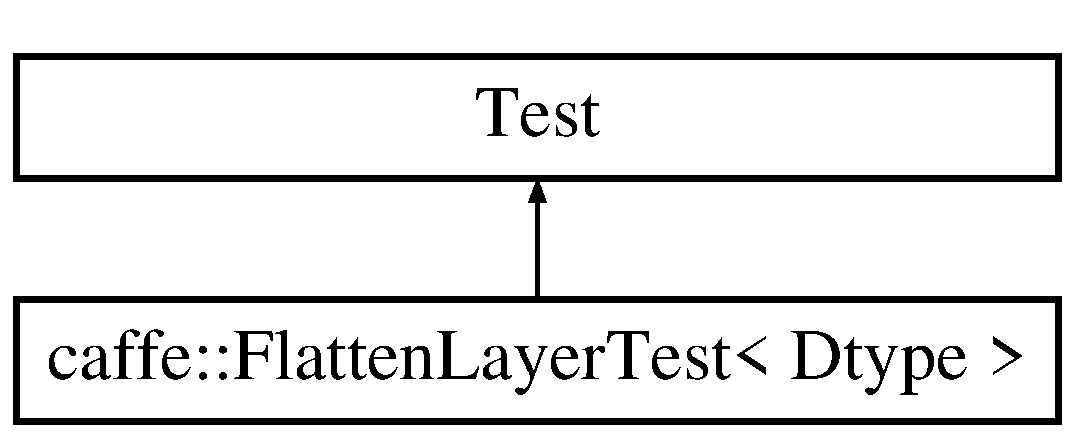
\includegraphics[height=2.000000cm]{classcaffe_1_1_flatten_layer_test}
\end{center}
\end{figure}
\subsection*{Protected Member Functions}
\begin{DoxyCompactItemize}
\item 
\hyperlink{classcaffe_1_1_flatten_layer_test_a58a9ad57ec7a4b131b713dd126a90198}{Flatten\+Layer\+Test} ()
\item 
virtual \hyperlink{classcaffe_1_1_flatten_layer_test_af3be11d061c8cf0d5e5f83c0aa0b7845}{$\sim$\+Flatten\+Layer\+Test} ()
\end{DoxyCompactItemize}
\subsection*{Protected Attributes}
\begin{DoxyCompactItemize}
\item 
\hyperlink{classcaffe_1_1_blob}{Blob}$<$ Dtype $>$ $\ast$const \hyperlink{classcaffe_1_1_flatten_layer_test_ac553bdfc0fcbf8c9e2c5f46f81a8bdca}{blob\+\_\+bottom\+\_\+}
\item 
\hyperlink{classcaffe_1_1_blob}{Blob}$<$ Dtype $>$ $\ast$const \hyperlink{classcaffe_1_1_flatten_layer_test_ab9f5b6129a7e55a87a5fea1f42deb1b4}{blob\+\_\+top\+\_\+}
\item 
vector$<$ \hyperlink{classcaffe_1_1_blob}{Blob}$<$ Dtype $>$ $\ast$ $>$ \hyperlink{classcaffe_1_1_flatten_layer_test_a65edcf7c3a3a0dc8cb5058dc2514a7fb}{blob\+\_\+bottom\+\_\+vec\+\_\+}
\item 
vector$<$ \hyperlink{classcaffe_1_1_blob}{Blob}$<$ Dtype $>$ $\ast$ $>$ \hyperlink{classcaffe_1_1_flatten_layer_test_aacf4562ee42d8d7a3336b0f5f7e1cfc1}{blob\+\_\+top\+\_\+vec\+\_\+}
\end{DoxyCompactItemize}


\subsection{Constructor \& Destructor Documentation}
\hypertarget{classcaffe_1_1_flatten_layer_test_a58a9ad57ec7a4b131b713dd126a90198}{\index{caffe\+::\+Flatten\+Layer\+Test@{caffe\+::\+Flatten\+Layer\+Test}!Flatten\+Layer\+Test@{Flatten\+Layer\+Test}}
\index{Flatten\+Layer\+Test@{Flatten\+Layer\+Test}!caffe\+::\+Flatten\+Layer\+Test@{caffe\+::\+Flatten\+Layer\+Test}}
\subsubsection[{Flatten\+Layer\+Test}]{\setlength{\rightskip}{0pt plus 5cm}template$<$typename Dtype $>$ {\bf caffe\+::\+Flatten\+Layer\+Test}$<$ Dtype $>$\+::{\bf Flatten\+Layer\+Test} (
\begin{DoxyParamCaption}
{}
\end{DoxyParamCaption}
)\hspace{0.3cm}{\ttfamily [inline]}, {\ttfamily [protected]}}}\label{classcaffe_1_1_flatten_layer_test_a58a9ad57ec7a4b131b713dd126a90198}
\hypertarget{classcaffe_1_1_flatten_layer_test_af3be11d061c8cf0d5e5f83c0aa0b7845}{\index{caffe\+::\+Flatten\+Layer\+Test@{caffe\+::\+Flatten\+Layer\+Test}!````~Flatten\+Layer\+Test@{$\sim$\+Flatten\+Layer\+Test}}
\index{````~Flatten\+Layer\+Test@{$\sim$\+Flatten\+Layer\+Test}!caffe\+::\+Flatten\+Layer\+Test@{caffe\+::\+Flatten\+Layer\+Test}}
\subsubsection[{$\sim$\+Flatten\+Layer\+Test}]{\setlength{\rightskip}{0pt plus 5cm}template$<$typename Dtype $>$ virtual {\bf caffe\+::\+Flatten\+Layer\+Test}$<$ Dtype $>$\+::$\sim${\bf Flatten\+Layer\+Test} (
\begin{DoxyParamCaption}
{}
\end{DoxyParamCaption}
)\hspace{0.3cm}{\ttfamily [inline]}, {\ttfamily [protected]}, {\ttfamily [virtual]}}}\label{classcaffe_1_1_flatten_layer_test_af3be11d061c8cf0d5e5f83c0aa0b7845}


\subsection{Member Data Documentation}
\hypertarget{classcaffe_1_1_flatten_layer_test_ac553bdfc0fcbf8c9e2c5f46f81a8bdca}{\index{caffe\+::\+Flatten\+Layer\+Test@{caffe\+::\+Flatten\+Layer\+Test}!blob\+\_\+bottom\+\_\+@{blob\+\_\+bottom\+\_\+}}
\index{blob\+\_\+bottom\+\_\+@{blob\+\_\+bottom\+\_\+}!caffe\+::\+Flatten\+Layer\+Test@{caffe\+::\+Flatten\+Layer\+Test}}
\subsubsection[{blob\+\_\+bottom\+\_\+}]{\setlength{\rightskip}{0pt plus 5cm}template$<$typename Dtype $>$ {\bf Blob}$<$Dtype$>$$\ast$ const {\bf caffe\+::\+Flatten\+Layer\+Test}$<$ Dtype $>$\+::blob\+\_\+bottom\+\_\+\hspace{0.3cm}{\ttfamily [protected]}}}\label{classcaffe_1_1_flatten_layer_test_ac553bdfc0fcbf8c9e2c5f46f81a8bdca}
\hypertarget{classcaffe_1_1_flatten_layer_test_a65edcf7c3a3a0dc8cb5058dc2514a7fb}{\index{caffe\+::\+Flatten\+Layer\+Test@{caffe\+::\+Flatten\+Layer\+Test}!blob\+\_\+bottom\+\_\+vec\+\_\+@{blob\+\_\+bottom\+\_\+vec\+\_\+}}
\index{blob\+\_\+bottom\+\_\+vec\+\_\+@{blob\+\_\+bottom\+\_\+vec\+\_\+}!caffe\+::\+Flatten\+Layer\+Test@{caffe\+::\+Flatten\+Layer\+Test}}
\subsubsection[{blob\+\_\+bottom\+\_\+vec\+\_\+}]{\setlength{\rightskip}{0pt plus 5cm}template$<$typename Dtype $>$ vector$<${\bf Blob}$<$Dtype$>$$\ast$$>$ {\bf caffe\+::\+Flatten\+Layer\+Test}$<$ Dtype $>$\+::blob\+\_\+bottom\+\_\+vec\+\_\+\hspace{0.3cm}{\ttfamily [protected]}}}\label{classcaffe_1_1_flatten_layer_test_a65edcf7c3a3a0dc8cb5058dc2514a7fb}
\hypertarget{classcaffe_1_1_flatten_layer_test_ab9f5b6129a7e55a87a5fea1f42deb1b4}{\index{caffe\+::\+Flatten\+Layer\+Test@{caffe\+::\+Flatten\+Layer\+Test}!blob\+\_\+top\+\_\+@{blob\+\_\+top\+\_\+}}
\index{blob\+\_\+top\+\_\+@{blob\+\_\+top\+\_\+}!caffe\+::\+Flatten\+Layer\+Test@{caffe\+::\+Flatten\+Layer\+Test}}
\subsubsection[{blob\+\_\+top\+\_\+}]{\setlength{\rightskip}{0pt plus 5cm}template$<$typename Dtype $>$ {\bf Blob}$<$Dtype$>$$\ast$ const {\bf caffe\+::\+Flatten\+Layer\+Test}$<$ Dtype $>$\+::blob\+\_\+top\+\_\+\hspace{0.3cm}{\ttfamily [protected]}}}\label{classcaffe_1_1_flatten_layer_test_ab9f5b6129a7e55a87a5fea1f42deb1b4}
\hypertarget{classcaffe_1_1_flatten_layer_test_aacf4562ee42d8d7a3336b0f5f7e1cfc1}{\index{caffe\+::\+Flatten\+Layer\+Test@{caffe\+::\+Flatten\+Layer\+Test}!blob\+\_\+top\+\_\+vec\+\_\+@{blob\+\_\+top\+\_\+vec\+\_\+}}
\index{blob\+\_\+top\+\_\+vec\+\_\+@{blob\+\_\+top\+\_\+vec\+\_\+}!caffe\+::\+Flatten\+Layer\+Test@{caffe\+::\+Flatten\+Layer\+Test}}
\subsubsection[{blob\+\_\+top\+\_\+vec\+\_\+}]{\setlength{\rightskip}{0pt plus 5cm}template$<$typename Dtype $>$ vector$<${\bf Blob}$<$Dtype$>$$\ast$$>$ {\bf caffe\+::\+Flatten\+Layer\+Test}$<$ Dtype $>$\+::blob\+\_\+top\+\_\+vec\+\_\+\hspace{0.3cm}{\ttfamily [protected]}}}\label{classcaffe_1_1_flatten_layer_test_aacf4562ee42d8d7a3336b0f5f7e1cfc1}


The documentation for this class was generated from the following file\+:\begin{DoxyCompactItemize}
\item 
src/caffe/test/\hyperlink{test__flatten__layer_8cpp}{test\+\_\+flatten\+\_\+layer.\+cpp}\end{DoxyCompactItemize}

\hypertarget{classcaffe_1_1_gaussian_filler}{\section{caffe\+:\+:Gaussian\+Filler$<$ Dtype $>$ Class Template Reference}
\label{classcaffe_1_1_gaussian_filler}\index{caffe\+::\+Gaussian\+Filler$<$ Dtype $>$@{caffe\+::\+Gaussian\+Filler$<$ Dtype $>$}}
}


{\ttfamily \#include $<$filler.\+hpp$>$}

Inheritance diagram for caffe\+:\+:Gaussian\+Filler$<$ Dtype $>$\+:\begin{figure}[H]
\begin{center}
\leavevmode
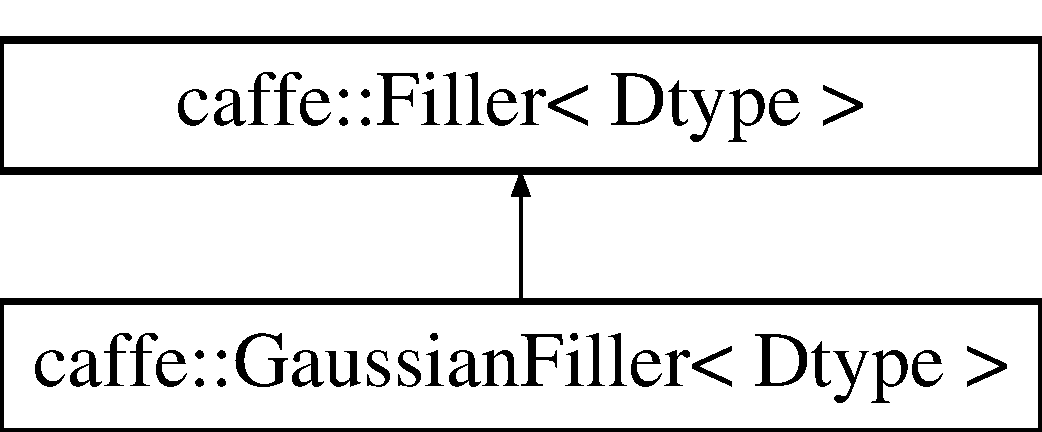
\includegraphics[height=2.000000cm]{classcaffe_1_1_gaussian_filler}
\end{center}
\end{figure}
\subsection*{Public Member Functions}
\begin{DoxyCompactItemize}
\item 
\hyperlink{classcaffe_1_1_gaussian_filler_a37a676739d64cf07b61767c99dd821b2}{Gaussian\+Filler} (const Filler\+Parameter \&param)
\item 
virtual void \hyperlink{classcaffe_1_1_gaussian_filler_ac45d5d0695521d7d71a4d5bccb659f21}{Fill} (\hyperlink{classcaffe_1_1_blob}{Blob}$<$ Dtype $>$ $\ast$blob)
\end{DoxyCompactItemize}
\subsection*{Protected Attributes}
\begin{DoxyCompactItemize}
\item 
shared\+\_\+ptr$<$ \hyperlink{classcaffe_1_1_synced_memory}{Synced\+Memory} $>$ \hyperlink{classcaffe_1_1_gaussian_filler_afec462a3671a2ad0cc09b6149be0b63c}{rand\+\_\+vec\+\_\+}
\end{DoxyCompactItemize}


\subsection{Constructor \& Destructor Documentation}
\hypertarget{classcaffe_1_1_gaussian_filler_a37a676739d64cf07b61767c99dd821b2}{\index{caffe\+::\+Gaussian\+Filler@{caffe\+::\+Gaussian\+Filler}!Gaussian\+Filler@{Gaussian\+Filler}}
\index{Gaussian\+Filler@{Gaussian\+Filler}!caffe\+::\+Gaussian\+Filler@{caffe\+::\+Gaussian\+Filler}}
\subsubsection[{Gaussian\+Filler}]{\setlength{\rightskip}{0pt plus 5cm}template$<$typename Dtype $>$ {\bf caffe\+::\+Gaussian\+Filler}$<$ Dtype $>$\+::{\bf Gaussian\+Filler} (
\begin{DoxyParamCaption}
\item[{const Filler\+Parameter \&}]{param}
\end{DoxyParamCaption}
)\hspace{0.3cm}{\ttfamily [inline]}, {\ttfamily [explicit]}}}\label{classcaffe_1_1_gaussian_filler_a37a676739d64cf07b61767c99dd821b2}


\subsection{Member Function Documentation}
\hypertarget{classcaffe_1_1_gaussian_filler_ac45d5d0695521d7d71a4d5bccb659f21}{\index{caffe\+::\+Gaussian\+Filler@{caffe\+::\+Gaussian\+Filler}!Fill@{Fill}}
\index{Fill@{Fill}!caffe\+::\+Gaussian\+Filler@{caffe\+::\+Gaussian\+Filler}}
\subsubsection[{Fill}]{\setlength{\rightskip}{0pt plus 5cm}template$<$typename Dtype $>$ virtual void {\bf caffe\+::\+Gaussian\+Filler}$<$ Dtype $>$\+::Fill (
\begin{DoxyParamCaption}
\item[{{\bf Blob}$<$ Dtype $>$ $\ast$}]{blob}
\end{DoxyParamCaption}
)\hspace{0.3cm}{\ttfamily [inline]}, {\ttfamily [virtual]}}}\label{classcaffe_1_1_gaussian_filler_ac45d5d0695521d7d71a4d5bccb659f21}


Implements \hyperlink{classcaffe_1_1_filler_acd02177b669381252a7c484f51432d30}{caffe\+::\+Filler$<$ Dtype $>$}.



\subsection{Member Data Documentation}
\hypertarget{classcaffe_1_1_gaussian_filler_afec462a3671a2ad0cc09b6149be0b63c}{\index{caffe\+::\+Gaussian\+Filler@{caffe\+::\+Gaussian\+Filler}!rand\+\_\+vec\+\_\+@{rand\+\_\+vec\+\_\+}}
\index{rand\+\_\+vec\+\_\+@{rand\+\_\+vec\+\_\+}!caffe\+::\+Gaussian\+Filler@{caffe\+::\+Gaussian\+Filler}}
\subsubsection[{rand\+\_\+vec\+\_\+}]{\setlength{\rightskip}{0pt plus 5cm}template$<$typename Dtype $>$ shared\+\_\+ptr$<${\bf Synced\+Memory}$>$ {\bf caffe\+::\+Gaussian\+Filler}$<$ Dtype $>$\+::rand\+\_\+vec\+\_\+\hspace{0.3cm}{\ttfamily [protected]}}}\label{classcaffe_1_1_gaussian_filler_afec462a3671a2ad0cc09b6149be0b63c}


The documentation for this class was generated from the following file\+:\begin{DoxyCompactItemize}
\item 
include/caffe/\hyperlink{filler_8hpp}{filler.\+hpp}\end{DoxyCompactItemize}

\hypertarget{classcaffe_1_1_gaussian_filler_test}{\section{caffe\+:\+:Gaussian\+Filler\+Test$<$ Dtype $>$ Class Template Reference}
\label{classcaffe_1_1_gaussian_filler_test}\index{caffe\+::\+Gaussian\+Filler\+Test$<$ Dtype $>$@{caffe\+::\+Gaussian\+Filler\+Test$<$ Dtype $>$}}
}
Inheritance diagram for caffe\+:\+:Gaussian\+Filler\+Test$<$ Dtype $>$\+:\begin{figure}[H]
\begin{center}
\leavevmode
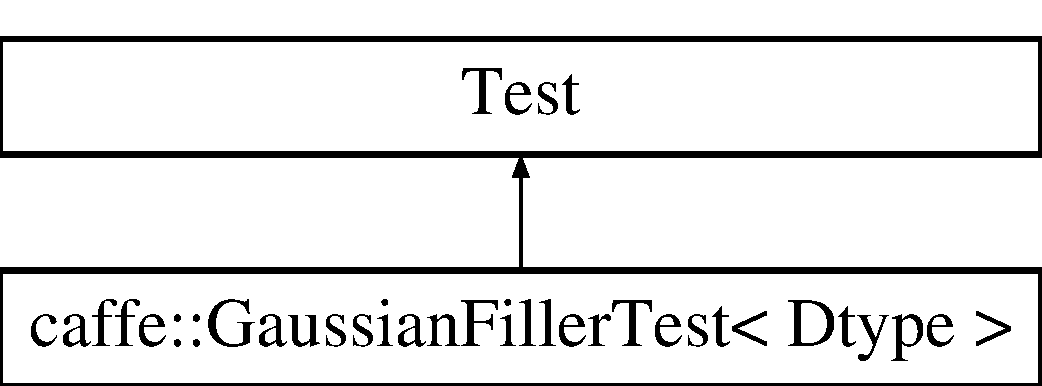
\includegraphics[height=2.000000cm]{classcaffe_1_1_gaussian_filler_test}
\end{center}
\end{figure}
\subsection*{Protected Member Functions}
\begin{DoxyCompactItemize}
\item 
\hyperlink{classcaffe_1_1_gaussian_filler_test_a9fd1e4e7a587870532c7b9bb55c979bc}{Gaussian\+Filler\+Test} ()
\item 
virtual \hyperlink{classcaffe_1_1_gaussian_filler_test_a242e8fbb3efc03492226cc43ca698041}{$\sim$\+Gaussian\+Filler\+Test} ()
\end{DoxyCompactItemize}
\subsection*{Protected Attributes}
\begin{DoxyCompactItemize}
\item 
\hyperlink{classcaffe_1_1_blob}{Blob}$<$ Dtype $>$ $\ast$const \hyperlink{classcaffe_1_1_gaussian_filler_test_a2bf1c6d059d5a2ddd346582a6e8e5f75}{blob\+\_\+}
\item 
Filler\+Parameter \hyperlink{classcaffe_1_1_gaussian_filler_test_a9043c61c0efe496faf5e8ba603d79395}{filler\+\_\+param\+\_\+}
\item 
shared\+\_\+ptr$<$ \hyperlink{classcaffe_1_1_gaussian_filler}{Gaussian\+Filler}\\*
$<$ Dtype $>$ $>$ \hyperlink{classcaffe_1_1_gaussian_filler_test_a742c237b4c3e81179d080f4122f2e92e}{filler\+\_\+}
\end{DoxyCompactItemize}


\subsection{Constructor \& Destructor Documentation}
\hypertarget{classcaffe_1_1_gaussian_filler_test_a9fd1e4e7a587870532c7b9bb55c979bc}{\index{caffe\+::\+Gaussian\+Filler\+Test@{caffe\+::\+Gaussian\+Filler\+Test}!Gaussian\+Filler\+Test@{Gaussian\+Filler\+Test}}
\index{Gaussian\+Filler\+Test@{Gaussian\+Filler\+Test}!caffe\+::\+Gaussian\+Filler\+Test@{caffe\+::\+Gaussian\+Filler\+Test}}
\subsubsection[{Gaussian\+Filler\+Test}]{\setlength{\rightskip}{0pt plus 5cm}template$<$typename Dtype $>$ {\bf caffe\+::\+Gaussian\+Filler\+Test}$<$ Dtype $>$\+::{\bf Gaussian\+Filler\+Test} (
\begin{DoxyParamCaption}
{}
\end{DoxyParamCaption}
)\hspace{0.3cm}{\ttfamily [inline]}, {\ttfamily [protected]}}}\label{classcaffe_1_1_gaussian_filler_test_a9fd1e4e7a587870532c7b9bb55c979bc}
\hypertarget{classcaffe_1_1_gaussian_filler_test_a242e8fbb3efc03492226cc43ca698041}{\index{caffe\+::\+Gaussian\+Filler\+Test@{caffe\+::\+Gaussian\+Filler\+Test}!````~Gaussian\+Filler\+Test@{$\sim$\+Gaussian\+Filler\+Test}}
\index{````~Gaussian\+Filler\+Test@{$\sim$\+Gaussian\+Filler\+Test}!caffe\+::\+Gaussian\+Filler\+Test@{caffe\+::\+Gaussian\+Filler\+Test}}
\subsubsection[{$\sim$\+Gaussian\+Filler\+Test}]{\setlength{\rightskip}{0pt plus 5cm}template$<$typename Dtype $>$ virtual {\bf caffe\+::\+Gaussian\+Filler\+Test}$<$ Dtype $>$\+::$\sim${\bf Gaussian\+Filler\+Test} (
\begin{DoxyParamCaption}
{}
\end{DoxyParamCaption}
)\hspace{0.3cm}{\ttfamily [inline]}, {\ttfamily [protected]}, {\ttfamily [virtual]}}}\label{classcaffe_1_1_gaussian_filler_test_a242e8fbb3efc03492226cc43ca698041}


\subsection{Member Data Documentation}
\hypertarget{classcaffe_1_1_gaussian_filler_test_a2bf1c6d059d5a2ddd346582a6e8e5f75}{\index{caffe\+::\+Gaussian\+Filler\+Test@{caffe\+::\+Gaussian\+Filler\+Test}!blob\+\_\+@{blob\+\_\+}}
\index{blob\+\_\+@{blob\+\_\+}!caffe\+::\+Gaussian\+Filler\+Test@{caffe\+::\+Gaussian\+Filler\+Test}}
\subsubsection[{blob\+\_\+}]{\setlength{\rightskip}{0pt plus 5cm}template$<$typename Dtype $>$ {\bf Blob}$<$Dtype$>$$\ast$ const {\bf caffe\+::\+Gaussian\+Filler\+Test}$<$ Dtype $>$\+::blob\+\_\+\hspace{0.3cm}{\ttfamily [protected]}}}\label{classcaffe_1_1_gaussian_filler_test_a2bf1c6d059d5a2ddd346582a6e8e5f75}
\hypertarget{classcaffe_1_1_gaussian_filler_test_a742c237b4c3e81179d080f4122f2e92e}{\index{caffe\+::\+Gaussian\+Filler\+Test@{caffe\+::\+Gaussian\+Filler\+Test}!filler\+\_\+@{filler\+\_\+}}
\index{filler\+\_\+@{filler\+\_\+}!caffe\+::\+Gaussian\+Filler\+Test@{caffe\+::\+Gaussian\+Filler\+Test}}
\subsubsection[{filler\+\_\+}]{\setlength{\rightskip}{0pt plus 5cm}template$<$typename Dtype $>$ shared\+\_\+ptr$<${\bf Gaussian\+Filler}$<$Dtype$>$ $>$ {\bf caffe\+::\+Gaussian\+Filler\+Test}$<$ Dtype $>$\+::filler\+\_\+\hspace{0.3cm}{\ttfamily [protected]}}}\label{classcaffe_1_1_gaussian_filler_test_a742c237b4c3e81179d080f4122f2e92e}
\hypertarget{classcaffe_1_1_gaussian_filler_test_a9043c61c0efe496faf5e8ba603d79395}{\index{caffe\+::\+Gaussian\+Filler\+Test@{caffe\+::\+Gaussian\+Filler\+Test}!filler\+\_\+param\+\_\+@{filler\+\_\+param\+\_\+}}
\index{filler\+\_\+param\+\_\+@{filler\+\_\+param\+\_\+}!caffe\+::\+Gaussian\+Filler\+Test@{caffe\+::\+Gaussian\+Filler\+Test}}
\subsubsection[{filler\+\_\+param\+\_\+}]{\setlength{\rightskip}{0pt plus 5cm}template$<$typename Dtype $>$ Filler\+Parameter {\bf caffe\+::\+Gaussian\+Filler\+Test}$<$ Dtype $>$\+::filler\+\_\+param\+\_\+\hspace{0.3cm}{\ttfamily [protected]}}}\label{classcaffe_1_1_gaussian_filler_test_a9043c61c0efe496faf5e8ba603d79395}


The documentation for this class was generated from the following file\+:\begin{DoxyCompactItemize}
\item 
src/caffe/test/\hyperlink{test__filler_8cpp}{test\+\_\+filler.\+cpp}\end{DoxyCompactItemize}

\hypertarget{classcaffe_1_1_gemm_test}{\section{caffe\+:\+:Gemm\+Test$<$ Dtype $>$ Class Template Reference}
\label{classcaffe_1_1_gemm_test}\index{caffe\+::\+Gemm\+Test$<$ Dtype $>$@{caffe\+::\+Gemm\+Test$<$ Dtype $>$}}
}
Inheritance diagram for caffe\+:\+:Gemm\+Test$<$ Dtype $>$\+:\begin{figure}[H]
\begin{center}
\leavevmode
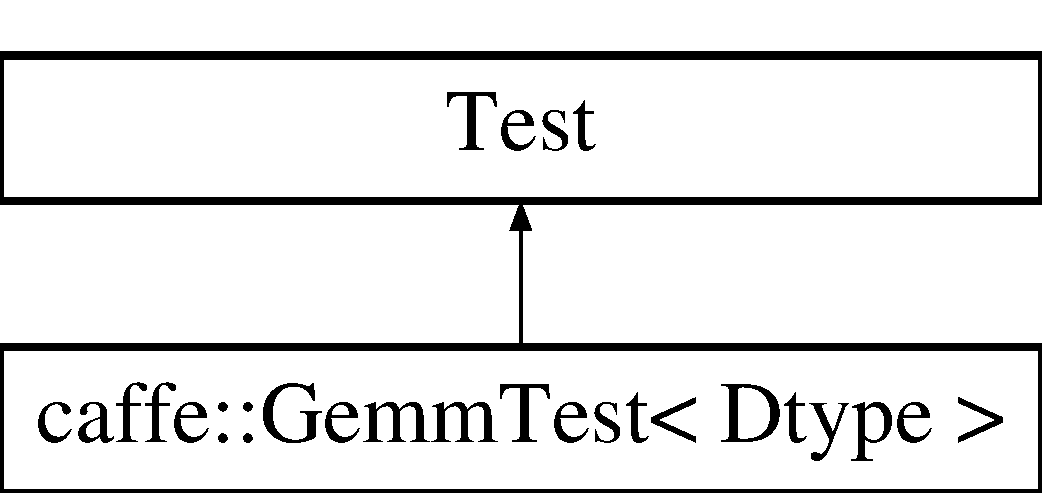
\includegraphics[height=2.000000cm]{classcaffe_1_1_gemm_test}
\end{center}
\end{figure}


The documentation for this class was generated from the following file\+:\begin{DoxyCompactItemize}
\item 
src/caffe/test/\hyperlink{test__util__blas_8cpp}{test\+\_\+util\+\_\+blas.\+cpp}\end{DoxyCompactItemize}

\hypertarget{classcaffe_1_1_caffe_1_1_r_n_g_1_1_generator}{\section{caffe\+:\+:Caffe\+:\+:R\+N\+G\+:\+:Generator Class Reference}
\label{classcaffe_1_1_caffe_1_1_r_n_g_1_1_generator}\index{caffe\+::\+Caffe\+::\+R\+N\+G\+::\+Generator@{caffe\+::\+Caffe\+::\+R\+N\+G\+::\+Generator}}
}
\subsection*{Public Member Functions}
\begin{DoxyCompactItemize}
\item 
\hyperlink{classcaffe_1_1_caffe_1_1_r_n_g_1_1_generator_a547a6adff11d675498a1fa3a55875d75}{Generator} ()
\item 
\hyperlink{classcaffe_1_1_caffe_1_1_r_n_g_1_1_generator_a25f41946ec93504bb7b132ef5072c0fc}{Generator} (unsigned int seed)
\item 
\hyperlink{namespacecaffe_aeff0d41eefd30caf64b0c9d03e142af3}{caffe\+::rng\+\_\+t} $\ast$ \hyperlink{classcaffe_1_1_caffe_1_1_r_n_g_1_1_generator_a43c97cbef420858b7f611396cc5093bf}{rng} ()
\end{DoxyCompactItemize}


\subsection{Constructor \& Destructor Documentation}
\hypertarget{classcaffe_1_1_caffe_1_1_r_n_g_1_1_generator_a547a6adff11d675498a1fa3a55875d75}{\index{caffe\+::\+Caffe\+::\+R\+N\+G\+::\+Generator@{caffe\+::\+Caffe\+::\+R\+N\+G\+::\+Generator}!Generator@{Generator}}
\index{Generator@{Generator}!caffe\+::\+Caffe\+::\+R\+N\+G\+::\+Generator@{caffe\+::\+Caffe\+::\+R\+N\+G\+::\+Generator}}
\subsubsection[{Generator}]{\setlength{\rightskip}{0pt plus 5cm}caffe\+::\+Caffe\+::\+R\+N\+G\+::\+Generator\+::\+Generator (
\begin{DoxyParamCaption}
{}
\end{DoxyParamCaption}
)\hspace{0.3cm}{\ttfamily [inline]}}}\label{classcaffe_1_1_caffe_1_1_r_n_g_1_1_generator_a547a6adff11d675498a1fa3a55875d75}
\hypertarget{classcaffe_1_1_caffe_1_1_r_n_g_1_1_generator_a25f41946ec93504bb7b132ef5072c0fc}{\index{caffe\+::\+Caffe\+::\+R\+N\+G\+::\+Generator@{caffe\+::\+Caffe\+::\+R\+N\+G\+::\+Generator}!Generator@{Generator}}
\index{Generator@{Generator}!caffe\+::\+Caffe\+::\+R\+N\+G\+::\+Generator@{caffe\+::\+Caffe\+::\+R\+N\+G\+::\+Generator}}
\subsubsection[{Generator}]{\setlength{\rightskip}{0pt plus 5cm}caffe\+::\+Caffe\+::\+R\+N\+G\+::\+Generator\+::\+Generator (
\begin{DoxyParamCaption}
\item[{unsigned int}]{seed}
\end{DoxyParamCaption}
)\hspace{0.3cm}{\ttfamily [inline]}, {\ttfamily [explicit]}}}\label{classcaffe_1_1_caffe_1_1_r_n_g_1_1_generator_a25f41946ec93504bb7b132ef5072c0fc}


\subsection{Member Function Documentation}
\hypertarget{classcaffe_1_1_caffe_1_1_r_n_g_1_1_generator_a43c97cbef420858b7f611396cc5093bf}{\index{caffe\+::\+Caffe\+::\+R\+N\+G\+::\+Generator@{caffe\+::\+Caffe\+::\+R\+N\+G\+::\+Generator}!rng@{rng}}
\index{rng@{rng}!caffe\+::\+Caffe\+::\+R\+N\+G\+::\+Generator@{caffe\+::\+Caffe\+::\+R\+N\+G\+::\+Generator}}
\subsubsection[{rng}]{\setlength{\rightskip}{0pt plus 5cm}{\bf caffe\+::rng\+\_\+t}$\ast$ caffe\+::\+Caffe\+::\+R\+N\+G\+::\+Generator\+::rng (
\begin{DoxyParamCaption}
{}
\end{DoxyParamCaption}
)\hspace{0.3cm}{\ttfamily [inline]}}}\label{classcaffe_1_1_caffe_1_1_r_n_g_1_1_generator_a43c97cbef420858b7f611396cc5093bf}


The documentation for this class was generated from the following file\+:\begin{DoxyCompactItemize}
\item 
src/caffe/\hyperlink{common_8cpp}{common.\+cpp}\end{DoxyCompactItemize}

\hypertarget{classcaffe_1_1_gradient_checker}{\section{caffe\+:\+:Gradient\+Checker$<$ Dtype $>$ Class Template Reference}
\label{classcaffe_1_1_gradient_checker}\index{caffe\+::\+Gradient\+Checker$<$ Dtype $>$@{caffe\+::\+Gradient\+Checker$<$ Dtype $>$}}
}


{\ttfamily \#include $<$test\+\_\+gradient\+\_\+check\+\_\+util.\+hpp$>$}

\subsection*{Public Member Functions}
\begin{DoxyCompactItemize}
\item 
\hyperlink{classcaffe_1_1_gradient_checker_a3669e5cf7ba11ee6858f628f7409fbdc}{Gradient\+Checker} (const Dtype stepsize, const Dtype threshold, const unsigned int seed=1701, const Dtype kink=0., const Dtype kink\+\_\+range=-\/1)
\item 
void \hyperlink{classcaffe_1_1_gradient_checker_acc5d8d420f39161eabcef0ba6985d2bb}{Check\+Gradient} (\hyperlink{classcaffe_1_1_layer}{Layer}$<$ Dtype $>$ $\ast$layer, vector$<$ \hyperlink{classcaffe_1_1_blob}{Blob}$<$ Dtype $>$ $\ast$ $>$ $\ast$bottom, vector$<$ \hyperlink{classcaffe_1_1_blob}{Blob}$<$ Dtype $>$ $\ast$ $>$ $\ast$top, int check\+\_\+bottom=-\/1)
\item 
void \hyperlink{classcaffe_1_1_gradient_checker_ac54a3abf29ba9fdec8c638b9d64bafda}{Check\+Gradient\+Exhaustive} (\hyperlink{classcaffe_1_1_layer}{Layer}$<$ Dtype $>$ $\ast$layer, vector$<$ \hyperlink{classcaffe_1_1_blob}{Blob}$<$ Dtype $>$ $\ast$ $>$ $\ast$bottom, vector$<$ \hyperlink{classcaffe_1_1_blob}{Blob}$<$ Dtype $>$ $\ast$ $>$ $\ast$top, int check\+\_\+bottom=-\/1)
\item 
void \hyperlink{classcaffe_1_1_gradient_checker_af91c345fb21a8ab832678f762a5c514b}{Check\+Gradient\+Eltwise} (\hyperlink{classcaffe_1_1_layer}{Layer}$<$ Dtype $>$ $\ast$layer, vector$<$ \hyperlink{classcaffe_1_1_blob}{Blob}$<$ Dtype $>$ $\ast$ $>$ $\ast$bottom, vector$<$ \hyperlink{classcaffe_1_1_blob}{Blob}$<$ Dtype $>$ $\ast$ $>$ $\ast$top)
\item 
void \hyperlink{classcaffe_1_1_gradient_checker_a29485303acb43364b6070db03dde91d6}{Check\+Gradient\+Single} (\hyperlink{classcaffe_1_1_layer}{Layer}$<$ Dtype $>$ $\ast$layer, vector$<$ \hyperlink{classcaffe_1_1_blob}{Blob}$<$ Dtype $>$ $\ast$ $>$ $\ast$bottom, vector$<$ \hyperlink{classcaffe_1_1_blob}{Blob}$<$ Dtype $>$ $\ast$ $>$ $\ast$top, int check\+\_\+bottom, int top\+\_\+id, int top\+\_\+data\+\_\+id, bool element\+\_\+wise=false)
\item 
void \hyperlink{classcaffe_1_1_gradient_checker_added2b064b65c97e1e5fdf93839d2d87}{Check\+Gradient\+Net} (const \hyperlink{classcaffe_1_1_net}{Net}$<$ Dtype $>$ \&net, const vector$<$ \hyperlink{classcaffe_1_1_blob}{Blob}$<$ Dtype $>$ $\ast$ $>$ \&input)
\end{DoxyCompactItemize}
\subsection*{Protected Member Functions}
\begin{DoxyCompactItemize}
\item 
Dtype \hyperlink{classcaffe_1_1_gradient_checker_a5a387a2f83155ed56ac065ea5e8598a5}{Get\+Obj\+And\+Gradient} (vector$<$ \hyperlink{classcaffe_1_1_blob}{Blob}$<$ Dtype $>$ $\ast$ $>$ $\ast$top, int top\+\_\+id=-\/1, int top\+\_\+data\+\_\+id=-\/1)
\end{DoxyCompactItemize}
\subsection*{Protected Attributes}
\begin{DoxyCompactItemize}
\item 
Dtype \hyperlink{classcaffe_1_1_gradient_checker_aaa427369839646baa465b09ead4ba5e7}{stepsize\+\_\+}
\item 
Dtype \hyperlink{classcaffe_1_1_gradient_checker_a2488c7b9f076c4578ba47cea46f8e947}{threshold\+\_\+}
\item 
unsigned int \hyperlink{classcaffe_1_1_gradient_checker_a2b5ddbc782ecee24eacf4e567e4bd954}{seed\+\_\+}
\item 
Dtype \hyperlink{classcaffe_1_1_gradient_checker_af6511d07455bbacdd61e79c33c13fbc9}{kink\+\_\+}
\item 
Dtype \hyperlink{classcaffe_1_1_gradient_checker_a827262b9c3ebcc0f20f9d135541a6c49}{kink\+\_\+range\+\_\+}
\end{DoxyCompactItemize}


\subsection{Constructor \& Destructor Documentation}
\hypertarget{classcaffe_1_1_gradient_checker_a3669e5cf7ba11ee6858f628f7409fbdc}{\index{caffe\+::\+Gradient\+Checker@{caffe\+::\+Gradient\+Checker}!Gradient\+Checker@{Gradient\+Checker}}
\index{Gradient\+Checker@{Gradient\+Checker}!caffe\+::\+Gradient\+Checker@{caffe\+::\+Gradient\+Checker}}
\subsubsection[{Gradient\+Checker}]{\setlength{\rightskip}{0pt plus 5cm}template$<$typename Dtype $>$ {\bf caffe\+::\+Gradient\+Checker}$<$ Dtype $>$\+::{\bf Gradient\+Checker} (
\begin{DoxyParamCaption}
\item[{const Dtype}]{stepsize, }
\item[{const Dtype}]{threshold, }
\item[{const unsigned int}]{seed = {\ttfamily 1701}, }
\item[{const Dtype}]{kink = {\ttfamily 0.}, }
\item[{const Dtype}]{kink\+\_\+range = {\ttfamily -\/1}}
\end{DoxyParamCaption}
)\hspace{0.3cm}{\ttfamily [inline]}}}\label{classcaffe_1_1_gradient_checker_a3669e5cf7ba11ee6858f628f7409fbdc}


\subsection{Member Function Documentation}
\hypertarget{classcaffe_1_1_gradient_checker_acc5d8d420f39161eabcef0ba6985d2bb}{\index{caffe\+::\+Gradient\+Checker@{caffe\+::\+Gradient\+Checker}!Check\+Gradient@{Check\+Gradient}}
\index{Check\+Gradient@{Check\+Gradient}!caffe\+::\+Gradient\+Checker@{caffe\+::\+Gradient\+Checker}}
\subsubsection[{Check\+Gradient}]{\setlength{\rightskip}{0pt plus 5cm}template$<$typename Dtype $>$ void {\bf caffe\+::\+Gradient\+Checker}$<$ Dtype $>$\+::Check\+Gradient (
\begin{DoxyParamCaption}
\item[{{\bf Layer}$<$ Dtype $>$ $\ast$}]{layer, }
\item[{vector$<$ {\bf Blob}$<$ Dtype $>$ $\ast$ $>$ $\ast$}]{bottom, }
\item[{vector$<$ {\bf Blob}$<$ Dtype $>$ $\ast$ $>$ $\ast$}]{top, }
\item[{int}]{check\+\_\+bottom = {\ttfamily -\/1}}
\end{DoxyParamCaption}
)\hspace{0.3cm}{\ttfamily [inline]}}}\label{classcaffe_1_1_gradient_checker_acc5d8d420f39161eabcef0ba6985d2bb}
\hypertarget{classcaffe_1_1_gradient_checker_af91c345fb21a8ab832678f762a5c514b}{\index{caffe\+::\+Gradient\+Checker@{caffe\+::\+Gradient\+Checker}!Check\+Gradient\+Eltwise@{Check\+Gradient\+Eltwise}}
\index{Check\+Gradient\+Eltwise@{Check\+Gradient\+Eltwise}!caffe\+::\+Gradient\+Checker@{caffe\+::\+Gradient\+Checker}}
\subsubsection[{Check\+Gradient\+Eltwise}]{\setlength{\rightskip}{0pt plus 5cm}template$<$typename Dtype $>$ void {\bf caffe\+::\+Gradient\+Checker}$<$ Dtype $>$\+::Check\+Gradient\+Eltwise (
\begin{DoxyParamCaption}
\item[{{\bf Layer}$<$ Dtype $>$ $\ast$}]{layer, }
\item[{vector$<$ {\bf Blob}$<$ Dtype $>$ $\ast$ $>$ $\ast$}]{bottom, }
\item[{vector$<$ {\bf Blob}$<$ Dtype $>$ $\ast$ $>$ $\ast$}]{top}
\end{DoxyParamCaption}
)}}\label{classcaffe_1_1_gradient_checker_af91c345fb21a8ab832678f762a5c514b}
\hypertarget{classcaffe_1_1_gradient_checker_ac54a3abf29ba9fdec8c638b9d64bafda}{\index{caffe\+::\+Gradient\+Checker@{caffe\+::\+Gradient\+Checker}!Check\+Gradient\+Exhaustive@{Check\+Gradient\+Exhaustive}}
\index{Check\+Gradient\+Exhaustive@{Check\+Gradient\+Exhaustive}!caffe\+::\+Gradient\+Checker@{caffe\+::\+Gradient\+Checker}}
\subsubsection[{Check\+Gradient\+Exhaustive}]{\setlength{\rightskip}{0pt plus 5cm}template$<$typename Dtype $>$ void {\bf caffe\+::\+Gradient\+Checker}$<$ Dtype $>$\+::Check\+Gradient\+Exhaustive (
\begin{DoxyParamCaption}
\item[{{\bf Layer}$<$ Dtype $>$ $\ast$}]{layer, }
\item[{vector$<$ {\bf Blob}$<$ Dtype $>$ $\ast$ $>$ $\ast$}]{bottom, }
\item[{vector$<$ {\bf Blob}$<$ Dtype $>$ $\ast$ $>$ $\ast$}]{top, }
\item[{int}]{check\+\_\+bottom = {\ttfamily -\/1}}
\end{DoxyParamCaption}
)}}\label{classcaffe_1_1_gradient_checker_ac54a3abf29ba9fdec8c638b9d64bafda}
\hypertarget{classcaffe_1_1_gradient_checker_added2b064b65c97e1e5fdf93839d2d87}{\index{caffe\+::\+Gradient\+Checker@{caffe\+::\+Gradient\+Checker}!Check\+Gradient\+Net@{Check\+Gradient\+Net}}
\index{Check\+Gradient\+Net@{Check\+Gradient\+Net}!caffe\+::\+Gradient\+Checker@{caffe\+::\+Gradient\+Checker}}
\subsubsection[{Check\+Gradient\+Net}]{\setlength{\rightskip}{0pt plus 5cm}template$<$typename Dtype $>$ void {\bf caffe\+::\+Gradient\+Checker}$<$ Dtype $>$\+::Check\+Gradient\+Net (
\begin{DoxyParamCaption}
\item[{const {\bf Net}$<$ Dtype $>$ \&}]{net, }
\item[{const vector$<$ {\bf Blob}$<$ Dtype $>$ $\ast$ $>$ \&}]{input}
\end{DoxyParamCaption}
)}}\label{classcaffe_1_1_gradient_checker_added2b064b65c97e1e5fdf93839d2d87}
\hypertarget{classcaffe_1_1_gradient_checker_a29485303acb43364b6070db03dde91d6}{\index{caffe\+::\+Gradient\+Checker@{caffe\+::\+Gradient\+Checker}!Check\+Gradient\+Single@{Check\+Gradient\+Single}}
\index{Check\+Gradient\+Single@{Check\+Gradient\+Single}!caffe\+::\+Gradient\+Checker@{caffe\+::\+Gradient\+Checker}}
\subsubsection[{Check\+Gradient\+Single}]{\setlength{\rightskip}{0pt plus 5cm}template$<$typename Dtype $>$ void {\bf caffe\+::\+Gradient\+Checker}$<$ Dtype $>$\+::Check\+Gradient\+Single (
\begin{DoxyParamCaption}
\item[{{\bf Layer}$<$ Dtype $>$ $\ast$}]{layer, }
\item[{vector$<$ {\bf Blob}$<$ Dtype $>$ $\ast$ $>$ $\ast$}]{bottom, }
\item[{vector$<$ {\bf Blob}$<$ Dtype $>$ $\ast$ $>$ $\ast$}]{top, }
\item[{int}]{check\+\_\+bottom, }
\item[{int}]{top\+\_\+id, }
\item[{int}]{top\+\_\+data\+\_\+id, }
\item[{bool}]{element\+\_\+wise = {\ttfamily false}}
\end{DoxyParamCaption}
)}}\label{classcaffe_1_1_gradient_checker_a29485303acb43364b6070db03dde91d6}
\hypertarget{classcaffe_1_1_gradient_checker_a5a387a2f83155ed56ac065ea5e8598a5}{\index{caffe\+::\+Gradient\+Checker@{caffe\+::\+Gradient\+Checker}!Get\+Obj\+And\+Gradient@{Get\+Obj\+And\+Gradient}}
\index{Get\+Obj\+And\+Gradient@{Get\+Obj\+And\+Gradient}!caffe\+::\+Gradient\+Checker@{caffe\+::\+Gradient\+Checker}}
\subsubsection[{Get\+Obj\+And\+Gradient}]{\setlength{\rightskip}{0pt plus 5cm}template$<$typename Dtype $>$ Dtype {\bf caffe\+::\+Gradient\+Checker}$<$ Dtype $>$\+::Get\+Obj\+And\+Gradient (
\begin{DoxyParamCaption}
\item[{vector$<$ {\bf Blob}$<$ Dtype $>$ $\ast$ $>$ $\ast$}]{top, }
\item[{int}]{top\+\_\+id = {\ttfamily -\/1}, }
\item[{int}]{top\+\_\+data\+\_\+id = {\ttfamily -\/1}}
\end{DoxyParamCaption}
)\hspace{0.3cm}{\ttfamily [protected]}}}\label{classcaffe_1_1_gradient_checker_a5a387a2f83155ed56ac065ea5e8598a5}


\subsection{Member Data Documentation}
\hypertarget{classcaffe_1_1_gradient_checker_af6511d07455bbacdd61e79c33c13fbc9}{\index{caffe\+::\+Gradient\+Checker@{caffe\+::\+Gradient\+Checker}!kink\+\_\+@{kink\+\_\+}}
\index{kink\+\_\+@{kink\+\_\+}!caffe\+::\+Gradient\+Checker@{caffe\+::\+Gradient\+Checker}}
\subsubsection[{kink\+\_\+}]{\setlength{\rightskip}{0pt plus 5cm}template$<$typename Dtype $>$ Dtype {\bf caffe\+::\+Gradient\+Checker}$<$ Dtype $>$\+::kink\+\_\+\hspace{0.3cm}{\ttfamily [protected]}}}\label{classcaffe_1_1_gradient_checker_af6511d07455bbacdd61e79c33c13fbc9}
\hypertarget{classcaffe_1_1_gradient_checker_a827262b9c3ebcc0f20f9d135541a6c49}{\index{caffe\+::\+Gradient\+Checker@{caffe\+::\+Gradient\+Checker}!kink\+\_\+range\+\_\+@{kink\+\_\+range\+\_\+}}
\index{kink\+\_\+range\+\_\+@{kink\+\_\+range\+\_\+}!caffe\+::\+Gradient\+Checker@{caffe\+::\+Gradient\+Checker}}
\subsubsection[{kink\+\_\+range\+\_\+}]{\setlength{\rightskip}{0pt plus 5cm}template$<$typename Dtype $>$ Dtype {\bf caffe\+::\+Gradient\+Checker}$<$ Dtype $>$\+::kink\+\_\+range\+\_\+\hspace{0.3cm}{\ttfamily [protected]}}}\label{classcaffe_1_1_gradient_checker_a827262b9c3ebcc0f20f9d135541a6c49}
\hypertarget{classcaffe_1_1_gradient_checker_a2b5ddbc782ecee24eacf4e567e4bd954}{\index{caffe\+::\+Gradient\+Checker@{caffe\+::\+Gradient\+Checker}!seed\+\_\+@{seed\+\_\+}}
\index{seed\+\_\+@{seed\+\_\+}!caffe\+::\+Gradient\+Checker@{caffe\+::\+Gradient\+Checker}}
\subsubsection[{seed\+\_\+}]{\setlength{\rightskip}{0pt plus 5cm}template$<$typename Dtype $>$ unsigned int {\bf caffe\+::\+Gradient\+Checker}$<$ Dtype $>$\+::seed\+\_\+\hspace{0.3cm}{\ttfamily [protected]}}}\label{classcaffe_1_1_gradient_checker_a2b5ddbc782ecee24eacf4e567e4bd954}
\hypertarget{classcaffe_1_1_gradient_checker_aaa427369839646baa465b09ead4ba5e7}{\index{caffe\+::\+Gradient\+Checker@{caffe\+::\+Gradient\+Checker}!stepsize\+\_\+@{stepsize\+\_\+}}
\index{stepsize\+\_\+@{stepsize\+\_\+}!caffe\+::\+Gradient\+Checker@{caffe\+::\+Gradient\+Checker}}
\subsubsection[{stepsize\+\_\+}]{\setlength{\rightskip}{0pt plus 5cm}template$<$typename Dtype $>$ Dtype {\bf caffe\+::\+Gradient\+Checker}$<$ Dtype $>$\+::stepsize\+\_\+\hspace{0.3cm}{\ttfamily [protected]}}}\label{classcaffe_1_1_gradient_checker_aaa427369839646baa465b09ead4ba5e7}
\hypertarget{classcaffe_1_1_gradient_checker_a2488c7b9f076c4578ba47cea46f8e947}{\index{caffe\+::\+Gradient\+Checker@{caffe\+::\+Gradient\+Checker}!threshold\+\_\+@{threshold\+\_\+}}
\index{threshold\+\_\+@{threshold\+\_\+}!caffe\+::\+Gradient\+Checker@{caffe\+::\+Gradient\+Checker}}
\subsubsection[{threshold\+\_\+}]{\setlength{\rightskip}{0pt plus 5cm}template$<$typename Dtype $>$ Dtype {\bf caffe\+::\+Gradient\+Checker}$<$ Dtype $>$\+::threshold\+\_\+\hspace{0.3cm}{\ttfamily [protected]}}}\label{classcaffe_1_1_gradient_checker_a2488c7b9f076c4578ba47cea46f8e947}


The documentation for this class was generated from the following file\+:\begin{DoxyCompactItemize}
\item 
src/caffe/test/\hyperlink{test__gradient__check__util_8hpp}{test\+\_\+gradient\+\_\+check\+\_\+util.\+hpp}\end{DoxyCompactItemize}

\hypertarget{classcaffe_1_1_h_d_f5_data_layer}{\section{caffe\+:\+:H\+D\+F5\+Data\+Layer$<$ Dtype $>$ Class Template Reference}
\label{classcaffe_1_1_h_d_f5_data_layer}\index{caffe\+::\+H\+D\+F5\+Data\+Layer$<$ Dtype $>$@{caffe\+::\+H\+D\+F5\+Data\+Layer$<$ Dtype $>$}}
}


{\ttfamily \#include $<$vision\+\_\+layers.\+hpp$>$}

Inheritance diagram for caffe\+:\+:H\+D\+F5\+Data\+Layer$<$ Dtype $>$\+:\begin{figure}[H]
\begin{center}
\leavevmode
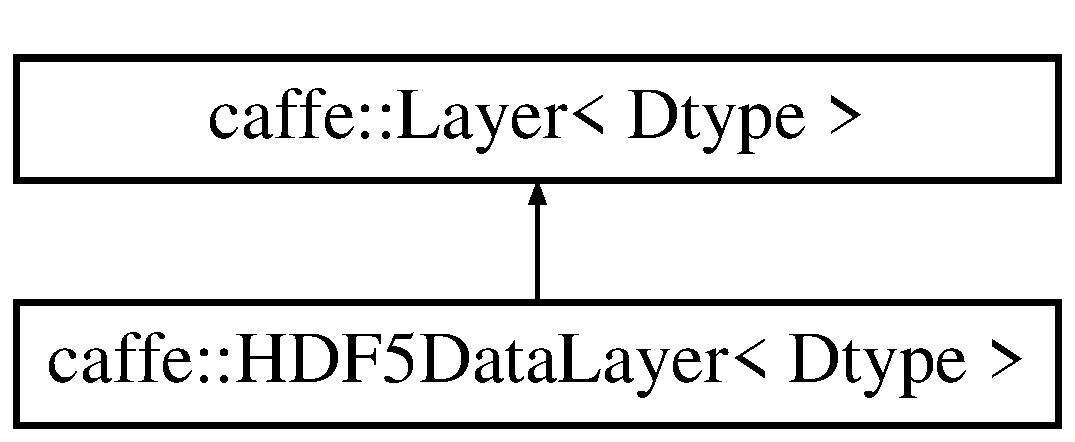
\includegraphics[height=2.000000cm]{classcaffe_1_1_h_d_f5_data_layer}
\end{center}
\end{figure}
\subsection*{Public Member Functions}
\begin{DoxyCompactItemize}
\item 
\hyperlink{classcaffe_1_1_h_d_f5_data_layer_abfc7dcc4f07c228eb0deb1e0dfae1a5f}{H\+D\+F5\+Data\+Layer} (const Layer\+Parameter \&param)
\item 
virtual \hyperlink{classcaffe_1_1_h_d_f5_data_layer_abadf2581e305508da149d1d799a3ec0a}{$\sim$\+H\+D\+F5\+Data\+Layer} ()
\item 
virtual void \hyperlink{classcaffe_1_1_h_d_f5_data_layer_a1b1786da3b00f367508d5f89d8d7dd59}{Set\+Up} (const vector$<$ \hyperlink{classcaffe_1_1_blob}{Blob}$<$ Dtype $>$ $\ast$ $>$ \&bottom, vector$<$ \hyperlink{classcaffe_1_1_blob}{Blob}$<$ Dtype $>$ $\ast$ $>$ $\ast$top)
\end{DoxyCompactItemize}
\subsection*{Protected Member Functions}
\begin{DoxyCompactItemize}
\item 
virtual Dtype \hyperlink{classcaffe_1_1_h_d_f5_data_layer_afb70fc6efdfffa6ee155abe193b53e3d}{Forward\+\_\+cpu} (const vector$<$ \hyperlink{classcaffe_1_1_blob}{Blob}$<$ Dtype $>$ $\ast$ $>$ \&bottom, vector$<$ \hyperlink{classcaffe_1_1_blob}{Blob}$<$ Dtype $>$ $\ast$ $>$ $\ast$top)
\item 
virtual Dtype \hyperlink{classcaffe_1_1_h_d_f5_data_layer_ab1413b32f9b5ad2182c7fd88b85240c3}{Forward\+\_\+gpu} (const vector$<$ \hyperlink{classcaffe_1_1_blob}{Blob}$<$ Dtype $>$ $\ast$ $>$ \&bottom, vector$<$ \hyperlink{classcaffe_1_1_blob}{Blob}$<$ Dtype $>$ $\ast$ $>$ $\ast$top)
\item 
virtual void \hyperlink{classcaffe_1_1_h_d_f5_data_layer_a2c44e32bcde368d4afbb2b9f68f4e3f8}{Backward\+\_\+cpu} (const vector$<$ \hyperlink{classcaffe_1_1_blob}{Blob}$<$ Dtype $>$ $\ast$ $>$ \&top, const bool propagate\+\_\+down, vector$<$ \hyperlink{classcaffe_1_1_blob}{Blob}$<$ Dtype $>$ $\ast$ $>$ $\ast$bottom)
\item 
virtual void \hyperlink{classcaffe_1_1_h_d_f5_data_layer_ac2528e6eea1bbcd1d6e3b0e35a7595b8}{Backward\+\_\+gpu} (const vector$<$ \hyperlink{classcaffe_1_1_blob}{Blob}$<$ Dtype $>$ $\ast$ $>$ \&top, const bool propagate\+\_\+down, vector$<$ \hyperlink{classcaffe_1_1_blob}{Blob}$<$ Dtype $>$ $\ast$ $>$ $\ast$bottom)
\item 
virtual void \hyperlink{classcaffe_1_1_h_d_f5_data_layer_a6fe59cc631f26f3323641ea480352119}{Load\+H\+D\+F5\+File\+Data} (const char $\ast$filename)
\end{DoxyCompactItemize}
\subsection*{Protected Attributes}
\begin{DoxyCompactItemize}
\item 
std\+::vector$<$ std\+::string $>$ \hyperlink{classcaffe_1_1_h_d_f5_data_layer_ae255f1e97fc8140bfeb7e3325f431f5a}{hdf\+\_\+filenames\+\_\+}
\item 
unsigned int \hyperlink{classcaffe_1_1_h_d_f5_data_layer_aa6154c78cd3f375f1bba8dc544362e59}{num\+\_\+files\+\_\+}
\item 
unsigned int \hyperlink{classcaffe_1_1_h_d_f5_data_layer_aa13b2e2012927eb433d007eb0cfcf8a7}{current\+\_\+file\+\_\+}
\item 
hsize\+\_\+t \hyperlink{classcaffe_1_1_h_d_f5_data_layer_a375f447a432bcd2ba94859b5b270ac96}{current\+\_\+row\+\_\+}
\item 
\hyperlink{classcaffe_1_1_blob}{Blob}$<$ Dtype $>$ \hyperlink{classcaffe_1_1_h_d_f5_data_layer_a9a70b53ef7435b4d565736fe8e3881ac}{data\+\_\+blob\+\_\+}
\item 
\hyperlink{classcaffe_1_1_blob}{Blob}$<$ Dtype $>$ \hyperlink{classcaffe_1_1_h_d_f5_data_layer_a15f4061897306968bb41c9300ab9250b}{label\+\_\+blob\+\_\+}
\end{DoxyCompactItemize}


\subsection{Constructor \& Destructor Documentation}
\hypertarget{classcaffe_1_1_h_d_f5_data_layer_abfc7dcc4f07c228eb0deb1e0dfae1a5f}{\index{caffe\+::\+H\+D\+F5\+Data\+Layer@{caffe\+::\+H\+D\+F5\+Data\+Layer}!H\+D\+F5\+Data\+Layer@{H\+D\+F5\+Data\+Layer}}
\index{H\+D\+F5\+Data\+Layer@{H\+D\+F5\+Data\+Layer}!caffe\+::\+H\+D\+F5\+Data\+Layer@{caffe\+::\+H\+D\+F5\+Data\+Layer}}
\subsubsection[{H\+D\+F5\+Data\+Layer}]{\setlength{\rightskip}{0pt plus 5cm}template$<$typename Dtype $>$ {\bf caffe\+::\+H\+D\+F5\+Data\+Layer}$<$ Dtype $>$\+::{\bf H\+D\+F5\+Data\+Layer} (
\begin{DoxyParamCaption}
\item[{const Layer\+Parameter \&}]{param}
\end{DoxyParamCaption}
)\hspace{0.3cm}{\ttfamily [inline]}, {\ttfamily [explicit]}}}\label{classcaffe_1_1_h_d_f5_data_layer_abfc7dcc4f07c228eb0deb1e0dfae1a5f}
\hypertarget{classcaffe_1_1_h_d_f5_data_layer_abadf2581e305508da149d1d799a3ec0a}{\index{caffe\+::\+H\+D\+F5\+Data\+Layer@{caffe\+::\+H\+D\+F5\+Data\+Layer}!````~H\+D\+F5\+Data\+Layer@{$\sim$\+H\+D\+F5\+Data\+Layer}}
\index{````~H\+D\+F5\+Data\+Layer@{$\sim$\+H\+D\+F5\+Data\+Layer}!caffe\+::\+H\+D\+F5\+Data\+Layer@{caffe\+::\+H\+D\+F5\+Data\+Layer}}
\subsubsection[{$\sim$\+H\+D\+F5\+Data\+Layer}]{\setlength{\rightskip}{0pt plus 5cm}template$<$typename Dtype $>$ {\bf caffe\+::\+H\+D\+F5\+Data\+Layer}$<$ Dtype $>$\+::$\sim${\bf H\+D\+F5\+Data\+Layer}$<$ Dtype $>$ (
\begin{DoxyParamCaption}
{}
\end{DoxyParamCaption}
)\hspace{0.3cm}{\ttfamily [virtual]}}}\label{classcaffe_1_1_h_d_f5_data_layer_abadf2581e305508da149d1d799a3ec0a}


\subsection{Member Function Documentation}
\hypertarget{classcaffe_1_1_h_d_f5_data_layer_a2c44e32bcde368d4afbb2b9f68f4e3f8}{\index{caffe\+::\+H\+D\+F5\+Data\+Layer@{caffe\+::\+H\+D\+F5\+Data\+Layer}!Backward\+\_\+cpu@{Backward\+\_\+cpu}}
\index{Backward\+\_\+cpu@{Backward\+\_\+cpu}!caffe\+::\+H\+D\+F5\+Data\+Layer@{caffe\+::\+H\+D\+F5\+Data\+Layer}}
\subsubsection[{Backward\+\_\+cpu}]{\setlength{\rightskip}{0pt plus 5cm}template$<$typename Dtype $>$ void {\bf caffe\+::\+H\+D\+F5\+Data\+Layer}$<$ Dtype $>$\+::Backward\+\_\+cpu (
\begin{DoxyParamCaption}
\item[{const vector$<$ {\bf Blob}$<$ Dtype $>$ $\ast$ $>$ \&}]{top, }
\item[{const bool}]{propagate\+\_\+down, }
\item[{vector$<$ {\bf Blob}$<$ Dtype $>$ $\ast$ $>$ $\ast$}]{bottom}
\end{DoxyParamCaption}
)\hspace{0.3cm}{\ttfamily [protected]}, {\ttfamily [virtual]}}}\label{classcaffe_1_1_h_d_f5_data_layer_a2c44e32bcde368d4afbb2b9f68f4e3f8}


Implements \hyperlink{classcaffe_1_1_layer_ac2d82011d076237c67997f63e7ee4b80}{caffe\+::\+Layer$<$ Dtype $>$}.

\hypertarget{classcaffe_1_1_h_d_f5_data_layer_ac2528e6eea1bbcd1d6e3b0e35a7595b8}{\index{caffe\+::\+H\+D\+F5\+Data\+Layer@{caffe\+::\+H\+D\+F5\+Data\+Layer}!Backward\+\_\+gpu@{Backward\+\_\+gpu}}
\index{Backward\+\_\+gpu@{Backward\+\_\+gpu}!caffe\+::\+H\+D\+F5\+Data\+Layer@{caffe\+::\+H\+D\+F5\+Data\+Layer}}
\subsubsection[{Backward\+\_\+gpu}]{\setlength{\rightskip}{0pt plus 5cm}template$<$typename Dtype $>$ void {\bf caffe\+::\+H\+D\+F5\+Data\+Layer}$<$ Dtype $>$\+::Backward\+\_\+gpu (
\begin{DoxyParamCaption}
\item[{const vector$<$ {\bf Blob}$<$ Dtype $>$ $\ast$ $>$ \&}]{top, }
\item[{const bool}]{propagate\+\_\+down, }
\item[{vector$<$ {\bf Blob}$<$ Dtype $>$ $\ast$ $>$ $\ast$}]{bottom}
\end{DoxyParamCaption}
)\hspace{0.3cm}{\ttfamily [protected]}, {\ttfamily [virtual]}}}\label{classcaffe_1_1_h_d_f5_data_layer_ac2528e6eea1bbcd1d6e3b0e35a7595b8}


Reimplemented from \hyperlink{classcaffe_1_1_layer_adf07ffe1f22d2fd2b1b0ff475ef5a64b}{caffe\+::\+Layer$<$ Dtype $>$}.

\hypertarget{classcaffe_1_1_h_d_f5_data_layer_afb70fc6efdfffa6ee155abe193b53e3d}{\index{caffe\+::\+H\+D\+F5\+Data\+Layer@{caffe\+::\+H\+D\+F5\+Data\+Layer}!Forward\+\_\+cpu@{Forward\+\_\+cpu}}
\index{Forward\+\_\+cpu@{Forward\+\_\+cpu}!caffe\+::\+H\+D\+F5\+Data\+Layer@{caffe\+::\+H\+D\+F5\+Data\+Layer}}
\subsubsection[{Forward\+\_\+cpu}]{\setlength{\rightskip}{0pt plus 5cm}template$<$typename Dtype $>$ Dtype {\bf caffe\+::\+H\+D\+F5\+Data\+Layer}$<$ Dtype $>$\+::Forward\+\_\+cpu (
\begin{DoxyParamCaption}
\item[{const vector$<$ {\bf Blob}$<$ Dtype $>$ $\ast$ $>$ \&}]{bottom, }
\item[{vector$<$ {\bf Blob}$<$ Dtype $>$ $\ast$ $>$ $\ast$}]{top}
\end{DoxyParamCaption}
)\hspace{0.3cm}{\ttfamily [protected]}, {\ttfamily [virtual]}}}\label{classcaffe_1_1_h_d_f5_data_layer_afb70fc6efdfffa6ee155abe193b53e3d}


Implements \hyperlink{classcaffe_1_1_layer_a8f7f61da3b8b3ca7f2394dee33873353}{caffe\+::\+Layer$<$ Dtype $>$}.

\hypertarget{classcaffe_1_1_h_d_f5_data_layer_ab1413b32f9b5ad2182c7fd88b85240c3}{\index{caffe\+::\+H\+D\+F5\+Data\+Layer@{caffe\+::\+H\+D\+F5\+Data\+Layer}!Forward\+\_\+gpu@{Forward\+\_\+gpu}}
\index{Forward\+\_\+gpu@{Forward\+\_\+gpu}!caffe\+::\+H\+D\+F5\+Data\+Layer@{caffe\+::\+H\+D\+F5\+Data\+Layer}}
\subsubsection[{Forward\+\_\+gpu}]{\setlength{\rightskip}{0pt plus 5cm}template$<$typename Dtype $>$ Dtype {\bf caffe\+::\+H\+D\+F5\+Data\+Layer}$<$ Dtype $>$\+::Forward\+\_\+gpu (
\begin{DoxyParamCaption}
\item[{const vector$<$ {\bf Blob}$<$ Dtype $>$ $\ast$ $>$ \&}]{bottom, }
\item[{vector$<$ {\bf Blob}$<$ Dtype $>$ $\ast$ $>$ $\ast$}]{top}
\end{DoxyParamCaption}
)\hspace{0.3cm}{\ttfamily [protected]}, {\ttfamily [virtual]}}}\label{classcaffe_1_1_h_d_f5_data_layer_ab1413b32f9b5ad2182c7fd88b85240c3}


Reimplemented from \hyperlink{classcaffe_1_1_layer_a2d78dbf5d8bc36928bd8f6fcfbafbcef}{caffe\+::\+Layer$<$ Dtype $>$}.

\hypertarget{classcaffe_1_1_h_d_f5_data_layer_a6fe59cc631f26f3323641ea480352119}{\index{caffe\+::\+H\+D\+F5\+Data\+Layer@{caffe\+::\+H\+D\+F5\+Data\+Layer}!Load\+H\+D\+F5\+File\+Data@{Load\+H\+D\+F5\+File\+Data}}
\index{Load\+H\+D\+F5\+File\+Data@{Load\+H\+D\+F5\+File\+Data}!caffe\+::\+H\+D\+F5\+Data\+Layer@{caffe\+::\+H\+D\+F5\+Data\+Layer}}
\subsubsection[{Load\+H\+D\+F5\+File\+Data}]{\setlength{\rightskip}{0pt plus 5cm}template$<$typename Dtype $>$ void {\bf caffe\+::\+H\+D\+F5\+Data\+Layer}$<$ Dtype $>$\+::Load\+H\+D\+F5\+File\+Data (
\begin{DoxyParamCaption}
\item[{const char $\ast$}]{filename}
\end{DoxyParamCaption}
)\hspace{0.3cm}{\ttfamily [protected]}, {\ttfamily [virtual]}}}\label{classcaffe_1_1_h_d_f5_data_layer_a6fe59cc631f26f3323641ea480352119}
\hypertarget{classcaffe_1_1_h_d_f5_data_layer_a1b1786da3b00f367508d5f89d8d7dd59}{\index{caffe\+::\+H\+D\+F5\+Data\+Layer@{caffe\+::\+H\+D\+F5\+Data\+Layer}!Set\+Up@{Set\+Up}}
\index{Set\+Up@{Set\+Up}!caffe\+::\+H\+D\+F5\+Data\+Layer@{caffe\+::\+H\+D\+F5\+Data\+Layer}}
\subsubsection[{Set\+Up}]{\setlength{\rightskip}{0pt plus 5cm}template$<$typename Dtype $>$ void {\bf caffe\+::\+H\+D\+F5\+Data\+Layer}$<$ Dtype $>$\+::Set\+Up (
\begin{DoxyParamCaption}
\item[{const vector$<$ {\bf Blob}$<$ Dtype $>$ $\ast$ $>$ \&}]{bottom, }
\item[{vector$<$ {\bf Blob}$<$ Dtype $>$ $\ast$ $>$ $\ast$}]{top}
\end{DoxyParamCaption}
)\hspace{0.3cm}{\ttfamily [virtual]}}}\label{classcaffe_1_1_h_d_f5_data_layer_a1b1786da3b00f367508d5f89d8d7dd59}


Implements \hyperlink{classcaffe_1_1_layer_abd13c6489c13953b4fbcfcf6880835d0}{caffe\+::\+Layer$<$ Dtype $>$}.



\subsection{Member Data Documentation}
\hypertarget{classcaffe_1_1_h_d_f5_data_layer_aa13b2e2012927eb433d007eb0cfcf8a7}{\index{caffe\+::\+H\+D\+F5\+Data\+Layer@{caffe\+::\+H\+D\+F5\+Data\+Layer}!current\+\_\+file\+\_\+@{current\+\_\+file\+\_\+}}
\index{current\+\_\+file\+\_\+@{current\+\_\+file\+\_\+}!caffe\+::\+H\+D\+F5\+Data\+Layer@{caffe\+::\+H\+D\+F5\+Data\+Layer}}
\subsubsection[{current\+\_\+file\+\_\+}]{\setlength{\rightskip}{0pt plus 5cm}template$<$typename Dtype $>$ unsigned int {\bf caffe\+::\+H\+D\+F5\+Data\+Layer}$<$ Dtype $>$\+::current\+\_\+file\+\_\+\hspace{0.3cm}{\ttfamily [protected]}}}\label{classcaffe_1_1_h_d_f5_data_layer_aa13b2e2012927eb433d007eb0cfcf8a7}
\hypertarget{classcaffe_1_1_h_d_f5_data_layer_a375f447a432bcd2ba94859b5b270ac96}{\index{caffe\+::\+H\+D\+F5\+Data\+Layer@{caffe\+::\+H\+D\+F5\+Data\+Layer}!current\+\_\+row\+\_\+@{current\+\_\+row\+\_\+}}
\index{current\+\_\+row\+\_\+@{current\+\_\+row\+\_\+}!caffe\+::\+H\+D\+F5\+Data\+Layer@{caffe\+::\+H\+D\+F5\+Data\+Layer}}
\subsubsection[{current\+\_\+row\+\_\+}]{\setlength{\rightskip}{0pt plus 5cm}template$<$typename Dtype $>$ hsize\+\_\+t {\bf caffe\+::\+H\+D\+F5\+Data\+Layer}$<$ Dtype $>$\+::current\+\_\+row\+\_\+\hspace{0.3cm}{\ttfamily [protected]}}}\label{classcaffe_1_1_h_d_f5_data_layer_a375f447a432bcd2ba94859b5b270ac96}
\hypertarget{classcaffe_1_1_h_d_f5_data_layer_a9a70b53ef7435b4d565736fe8e3881ac}{\index{caffe\+::\+H\+D\+F5\+Data\+Layer@{caffe\+::\+H\+D\+F5\+Data\+Layer}!data\+\_\+blob\+\_\+@{data\+\_\+blob\+\_\+}}
\index{data\+\_\+blob\+\_\+@{data\+\_\+blob\+\_\+}!caffe\+::\+H\+D\+F5\+Data\+Layer@{caffe\+::\+H\+D\+F5\+Data\+Layer}}
\subsubsection[{data\+\_\+blob\+\_\+}]{\setlength{\rightskip}{0pt plus 5cm}template$<$typename Dtype $>$ {\bf Blob}$<$Dtype$>$ {\bf caffe\+::\+H\+D\+F5\+Data\+Layer}$<$ Dtype $>$\+::data\+\_\+blob\+\_\+\hspace{0.3cm}{\ttfamily [protected]}}}\label{classcaffe_1_1_h_d_f5_data_layer_a9a70b53ef7435b4d565736fe8e3881ac}
\hypertarget{classcaffe_1_1_h_d_f5_data_layer_ae255f1e97fc8140bfeb7e3325f431f5a}{\index{caffe\+::\+H\+D\+F5\+Data\+Layer@{caffe\+::\+H\+D\+F5\+Data\+Layer}!hdf\+\_\+filenames\+\_\+@{hdf\+\_\+filenames\+\_\+}}
\index{hdf\+\_\+filenames\+\_\+@{hdf\+\_\+filenames\+\_\+}!caffe\+::\+H\+D\+F5\+Data\+Layer@{caffe\+::\+H\+D\+F5\+Data\+Layer}}
\subsubsection[{hdf\+\_\+filenames\+\_\+}]{\setlength{\rightskip}{0pt plus 5cm}template$<$typename Dtype $>$ std\+::vector$<$std\+::string$>$ {\bf caffe\+::\+H\+D\+F5\+Data\+Layer}$<$ Dtype $>$\+::hdf\+\_\+filenames\+\_\+\hspace{0.3cm}{\ttfamily [protected]}}}\label{classcaffe_1_1_h_d_f5_data_layer_ae255f1e97fc8140bfeb7e3325f431f5a}
\hypertarget{classcaffe_1_1_h_d_f5_data_layer_a15f4061897306968bb41c9300ab9250b}{\index{caffe\+::\+H\+D\+F5\+Data\+Layer@{caffe\+::\+H\+D\+F5\+Data\+Layer}!label\+\_\+blob\+\_\+@{label\+\_\+blob\+\_\+}}
\index{label\+\_\+blob\+\_\+@{label\+\_\+blob\+\_\+}!caffe\+::\+H\+D\+F5\+Data\+Layer@{caffe\+::\+H\+D\+F5\+Data\+Layer}}
\subsubsection[{label\+\_\+blob\+\_\+}]{\setlength{\rightskip}{0pt plus 5cm}template$<$typename Dtype $>$ {\bf Blob}$<$Dtype$>$ {\bf caffe\+::\+H\+D\+F5\+Data\+Layer}$<$ Dtype $>$\+::label\+\_\+blob\+\_\+\hspace{0.3cm}{\ttfamily [protected]}}}\label{classcaffe_1_1_h_d_f5_data_layer_a15f4061897306968bb41c9300ab9250b}
\hypertarget{classcaffe_1_1_h_d_f5_data_layer_aa6154c78cd3f375f1bba8dc544362e59}{\index{caffe\+::\+H\+D\+F5\+Data\+Layer@{caffe\+::\+H\+D\+F5\+Data\+Layer}!num\+\_\+files\+\_\+@{num\+\_\+files\+\_\+}}
\index{num\+\_\+files\+\_\+@{num\+\_\+files\+\_\+}!caffe\+::\+H\+D\+F5\+Data\+Layer@{caffe\+::\+H\+D\+F5\+Data\+Layer}}
\subsubsection[{num\+\_\+files\+\_\+}]{\setlength{\rightskip}{0pt plus 5cm}template$<$typename Dtype $>$ unsigned int {\bf caffe\+::\+H\+D\+F5\+Data\+Layer}$<$ Dtype $>$\+::num\+\_\+files\+\_\+\hspace{0.3cm}{\ttfamily [protected]}}}\label{classcaffe_1_1_h_d_f5_data_layer_aa6154c78cd3f375f1bba8dc544362e59}


The documentation for this class was generated from the following files\+:\begin{DoxyCompactItemize}
\item 
include/caffe/\hyperlink{vision__layers_8hpp}{vision\+\_\+layers.\+hpp}\item 
src/caffe/layers/\hyperlink{hdf5__data__layer_8cpp}{hdf5\+\_\+data\+\_\+layer.\+cpp}\item 
src/caffe/layers/\hyperlink{hdf5__data__layer_8cu}{hdf5\+\_\+data\+\_\+layer.\+cu}\end{DoxyCompactItemize}

\hypertarget{classcaffe_1_1_h_d_f5_data_layer_test}{\section{caffe\+:\+:H\+D\+F5\+Data\+Layer\+Test$<$ Dtype $>$ Class Template Reference}
\label{classcaffe_1_1_h_d_f5_data_layer_test}\index{caffe\+::\+H\+D\+F5\+Data\+Layer\+Test$<$ Dtype $>$@{caffe\+::\+H\+D\+F5\+Data\+Layer\+Test$<$ Dtype $>$}}
}
Inheritance diagram for caffe\+:\+:H\+D\+F5\+Data\+Layer\+Test$<$ Dtype $>$\+:\begin{figure}[H]
\begin{center}
\leavevmode
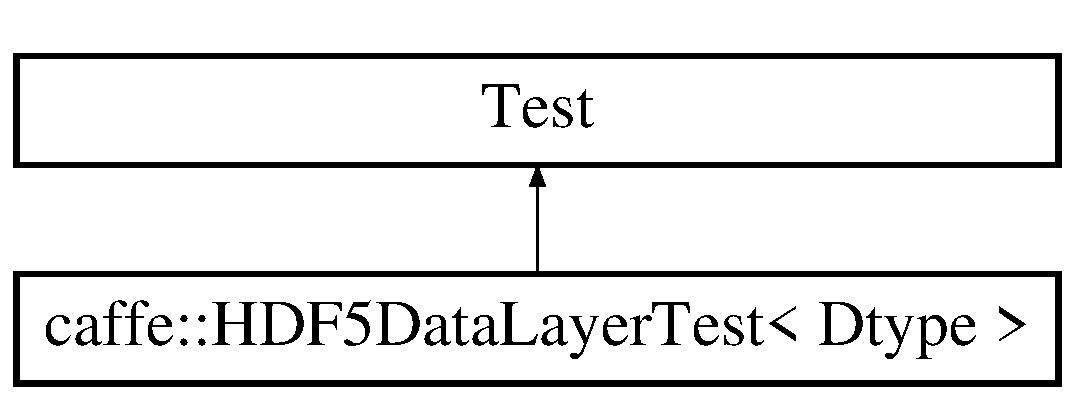
\includegraphics[height=2.000000cm]{classcaffe_1_1_h_d_f5_data_layer_test}
\end{center}
\end{figure}
\subsection*{Protected Member Functions}
\begin{DoxyCompactItemize}
\item 
\hyperlink{classcaffe_1_1_h_d_f5_data_layer_test_a193e15cc2ccd1437aa0aa5096d5dfde6}{H\+D\+F5\+Data\+Layer\+Test} ()
\item 
virtual void \hyperlink{classcaffe_1_1_h_d_f5_data_layer_test_a87eaa2af48eba154aaf5a5429708c7b1}{Set\+Up} ()
\item 
virtual \hyperlink{classcaffe_1_1_h_d_f5_data_layer_test_a3a1a5bd011ab7f9514cb2fbe40612f7e}{$\sim$\+H\+D\+F5\+Data\+Layer\+Test} ()
\end{DoxyCompactItemize}
\subsection*{Protected Attributes}
\begin{DoxyCompactItemize}
\item 
string $\ast$ \hyperlink{classcaffe_1_1_h_d_f5_data_layer_test_a7f63b15d92f052d045c969e74ad8ed5d}{filename}
\item 
\hyperlink{classcaffe_1_1_blob}{Blob}$<$ Dtype $>$ $\ast$const \hyperlink{classcaffe_1_1_h_d_f5_data_layer_test_a4e051fd65360f35354b864e33ae74eaa}{blob\+\_\+top\+\_\+data\+\_\+}
\item 
\hyperlink{classcaffe_1_1_blob}{Blob}$<$ Dtype $>$ $\ast$const \hyperlink{classcaffe_1_1_h_d_f5_data_layer_test_afb89ea13ccf6f75de384f703c9444174}{blob\+\_\+top\+\_\+label\+\_\+}
\item 
vector$<$ \hyperlink{classcaffe_1_1_blob}{Blob}$<$ Dtype $>$ $\ast$ $>$ \hyperlink{classcaffe_1_1_h_d_f5_data_layer_test_a68f3f644d32f341c09cab346701df1e6}{blob\+\_\+bottom\+\_\+vec\+\_\+}
\item 
vector$<$ \hyperlink{classcaffe_1_1_blob}{Blob}$<$ Dtype $>$ $\ast$ $>$ \hyperlink{classcaffe_1_1_h_d_f5_data_layer_test_add8fb70dc419407a8e0ca8a78640c380}{blob\+\_\+top\+\_\+vec\+\_\+}
\end{DoxyCompactItemize}


\subsection{Constructor \& Destructor Documentation}
\hypertarget{classcaffe_1_1_h_d_f5_data_layer_test_a193e15cc2ccd1437aa0aa5096d5dfde6}{\index{caffe\+::\+H\+D\+F5\+Data\+Layer\+Test@{caffe\+::\+H\+D\+F5\+Data\+Layer\+Test}!H\+D\+F5\+Data\+Layer\+Test@{H\+D\+F5\+Data\+Layer\+Test}}
\index{H\+D\+F5\+Data\+Layer\+Test@{H\+D\+F5\+Data\+Layer\+Test}!caffe\+::\+H\+D\+F5\+Data\+Layer\+Test@{caffe\+::\+H\+D\+F5\+Data\+Layer\+Test}}
\subsubsection[{H\+D\+F5\+Data\+Layer\+Test}]{\setlength{\rightskip}{0pt plus 5cm}template$<$typename Dtype $>$ {\bf caffe\+::\+H\+D\+F5\+Data\+Layer\+Test}$<$ Dtype $>$\+::{\bf H\+D\+F5\+Data\+Layer\+Test} (
\begin{DoxyParamCaption}
{}
\end{DoxyParamCaption}
)\hspace{0.3cm}{\ttfamily [inline]}, {\ttfamily [protected]}}}\label{classcaffe_1_1_h_d_f5_data_layer_test_a193e15cc2ccd1437aa0aa5096d5dfde6}
\hypertarget{classcaffe_1_1_h_d_f5_data_layer_test_a3a1a5bd011ab7f9514cb2fbe40612f7e}{\index{caffe\+::\+H\+D\+F5\+Data\+Layer\+Test@{caffe\+::\+H\+D\+F5\+Data\+Layer\+Test}!````~H\+D\+F5\+Data\+Layer\+Test@{$\sim$\+H\+D\+F5\+Data\+Layer\+Test}}
\index{````~H\+D\+F5\+Data\+Layer\+Test@{$\sim$\+H\+D\+F5\+Data\+Layer\+Test}!caffe\+::\+H\+D\+F5\+Data\+Layer\+Test@{caffe\+::\+H\+D\+F5\+Data\+Layer\+Test}}
\subsubsection[{$\sim$\+H\+D\+F5\+Data\+Layer\+Test}]{\setlength{\rightskip}{0pt plus 5cm}template$<$typename Dtype $>$ virtual {\bf caffe\+::\+H\+D\+F5\+Data\+Layer\+Test}$<$ Dtype $>$\+::$\sim${\bf H\+D\+F5\+Data\+Layer\+Test} (
\begin{DoxyParamCaption}
{}
\end{DoxyParamCaption}
)\hspace{0.3cm}{\ttfamily [inline]}, {\ttfamily [protected]}, {\ttfamily [virtual]}}}\label{classcaffe_1_1_h_d_f5_data_layer_test_a3a1a5bd011ab7f9514cb2fbe40612f7e}


\subsection{Member Function Documentation}
\hypertarget{classcaffe_1_1_h_d_f5_data_layer_test_a87eaa2af48eba154aaf5a5429708c7b1}{\index{caffe\+::\+H\+D\+F5\+Data\+Layer\+Test@{caffe\+::\+H\+D\+F5\+Data\+Layer\+Test}!Set\+Up@{Set\+Up}}
\index{Set\+Up@{Set\+Up}!caffe\+::\+H\+D\+F5\+Data\+Layer\+Test@{caffe\+::\+H\+D\+F5\+Data\+Layer\+Test}}
\subsubsection[{Set\+Up}]{\setlength{\rightskip}{0pt plus 5cm}template$<$typename Dtype $>$ virtual void {\bf caffe\+::\+H\+D\+F5\+Data\+Layer\+Test}$<$ Dtype $>$\+::Set\+Up (
\begin{DoxyParamCaption}
{}
\end{DoxyParamCaption}
)\hspace{0.3cm}{\ttfamily [inline]}, {\ttfamily [protected]}, {\ttfamily [virtual]}}}\label{classcaffe_1_1_h_d_f5_data_layer_test_a87eaa2af48eba154aaf5a5429708c7b1}


\subsection{Member Data Documentation}
\hypertarget{classcaffe_1_1_h_d_f5_data_layer_test_a68f3f644d32f341c09cab346701df1e6}{\index{caffe\+::\+H\+D\+F5\+Data\+Layer\+Test@{caffe\+::\+H\+D\+F5\+Data\+Layer\+Test}!blob\+\_\+bottom\+\_\+vec\+\_\+@{blob\+\_\+bottom\+\_\+vec\+\_\+}}
\index{blob\+\_\+bottom\+\_\+vec\+\_\+@{blob\+\_\+bottom\+\_\+vec\+\_\+}!caffe\+::\+H\+D\+F5\+Data\+Layer\+Test@{caffe\+::\+H\+D\+F5\+Data\+Layer\+Test}}
\subsubsection[{blob\+\_\+bottom\+\_\+vec\+\_\+}]{\setlength{\rightskip}{0pt plus 5cm}template$<$typename Dtype $>$ vector$<${\bf Blob}$<$Dtype$>$$\ast$$>$ {\bf caffe\+::\+H\+D\+F5\+Data\+Layer\+Test}$<$ Dtype $>$\+::blob\+\_\+bottom\+\_\+vec\+\_\+\hspace{0.3cm}{\ttfamily [protected]}}}\label{classcaffe_1_1_h_d_f5_data_layer_test_a68f3f644d32f341c09cab346701df1e6}
\hypertarget{classcaffe_1_1_h_d_f5_data_layer_test_a4e051fd65360f35354b864e33ae74eaa}{\index{caffe\+::\+H\+D\+F5\+Data\+Layer\+Test@{caffe\+::\+H\+D\+F5\+Data\+Layer\+Test}!blob\+\_\+top\+\_\+data\+\_\+@{blob\+\_\+top\+\_\+data\+\_\+}}
\index{blob\+\_\+top\+\_\+data\+\_\+@{blob\+\_\+top\+\_\+data\+\_\+}!caffe\+::\+H\+D\+F5\+Data\+Layer\+Test@{caffe\+::\+H\+D\+F5\+Data\+Layer\+Test}}
\subsubsection[{blob\+\_\+top\+\_\+data\+\_\+}]{\setlength{\rightskip}{0pt plus 5cm}template$<$typename Dtype $>$ {\bf Blob}$<$Dtype$>$$\ast$ const {\bf caffe\+::\+H\+D\+F5\+Data\+Layer\+Test}$<$ Dtype $>$\+::blob\+\_\+top\+\_\+data\+\_\+\hspace{0.3cm}{\ttfamily [protected]}}}\label{classcaffe_1_1_h_d_f5_data_layer_test_a4e051fd65360f35354b864e33ae74eaa}
\hypertarget{classcaffe_1_1_h_d_f5_data_layer_test_afb89ea13ccf6f75de384f703c9444174}{\index{caffe\+::\+H\+D\+F5\+Data\+Layer\+Test@{caffe\+::\+H\+D\+F5\+Data\+Layer\+Test}!blob\+\_\+top\+\_\+label\+\_\+@{blob\+\_\+top\+\_\+label\+\_\+}}
\index{blob\+\_\+top\+\_\+label\+\_\+@{blob\+\_\+top\+\_\+label\+\_\+}!caffe\+::\+H\+D\+F5\+Data\+Layer\+Test@{caffe\+::\+H\+D\+F5\+Data\+Layer\+Test}}
\subsubsection[{blob\+\_\+top\+\_\+label\+\_\+}]{\setlength{\rightskip}{0pt plus 5cm}template$<$typename Dtype $>$ {\bf Blob}$<$Dtype$>$$\ast$ const {\bf caffe\+::\+H\+D\+F5\+Data\+Layer\+Test}$<$ Dtype $>$\+::blob\+\_\+top\+\_\+label\+\_\+\hspace{0.3cm}{\ttfamily [protected]}}}\label{classcaffe_1_1_h_d_f5_data_layer_test_afb89ea13ccf6f75de384f703c9444174}
\hypertarget{classcaffe_1_1_h_d_f5_data_layer_test_add8fb70dc419407a8e0ca8a78640c380}{\index{caffe\+::\+H\+D\+F5\+Data\+Layer\+Test@{caffe\+::\+H\+D\+F5\+Data\+Layer\+Test}!blob\+\_\+top\+\_\+vec\+\_\+@{blob\+\_\+top\+\_\+vec\+\_\+}}
\index{blob\+\_\+top\+\_\+vec\+\_\+@{blob\+\_\+top\+\_\+vec\+\_\+}!caffe\+::\+H\+D\+F5\+Data\+Layer\+Test@{caffe\+::\+H\+D\+F5\+Data\+Layer\+Test}}
\subsubsection[{blob\+\_\+top\+\_\+vec\+\_\+}]{\setlength{\rightskip}{0pt plus 5cm}template$<$typename Dtype $>$ vector$<${\bf Blob}$<$Dtype$>$$\ast$$>$ {\bf caffe\+::\+H\+D\+F5\+Data\+Layer\+Test}$<$ Dtype $>$\+::blob\+\_\+top\+\_\+vec\+\_\+\hspace{0.3cm}{\ttfamily [protected]}}}\label{classcaffe_1_1_h_d_f5_data_layer_test_add8fb70dc419407a8e0ca8a78640c380}
\hypertarget{classcaffe_1_1_h_d_f5_data_layer_test_a7f63b15d92f052d045c969e74ad8ed5d}{\index{caffe\+::\+H\+D\+F5\+Data\+Layer\+Test@{caffe\+::\+H\+D\+F5\+Data\+Layer\+Test}!filename@{filename}}
\index{filename@{filename}!caffe\+::\+H\+D\+F5\+Data\+Layer\+Test@{caffe\+::\+H\+D\+F5\+Data\+Layer\+Test}}
\subsubsection[{filename}]{\setlength{\rightskip}{0pt plus 5cm}template$<$typename Dtype $>$ string$\ast$ {\bf caffe\+::\+H\+D\+F5\+Data\+Layer\+Test}$<$ Dtype $>$\+::filename\hspace{0.3cm}{\ttfamily [protected]}}}\label{classcaffe_1_1_h_d_f5_data_layer_test_a7f63b15d92f052d045c969e74ad8ed5d}


The documentation for this class was generated from the following file\+:\begin{DoxyCompactItemize}
\item 
src/caffe/test/\hyperlink{test__hdf5data__layer_8cpp}{test\+\_\+hdf5data\+\_\+layer.\+cpp}\end{DoxyCompactItemize}

\hypertarget{classcaffe_1_1_h_d_f5_output_layer}{\section{caffe\+:\+:H\+D\+F5\+Output\+Layer$<$ Dtype $>$ Class Template Reference}
\label{classcaffe_1_1_h_d_f5_output_layer}\index{caffe\+::\+H\+D\+F5\+Output\+Layer$<$ Dtype $>$@{caffe\+::\+H\+D\+F5\+Output\+Layer$<$ Dtype $>$}}
}


{\ttfamily \#include $<$vision\+\_\+layers.\+hpp$>$}

Inheritance diagram for caffe\+:\+:H\+D\+F5\+Output\+Layer$<$ Dtype $>$\+:\begin{figure}[H]
\begin{center}
\leavevmode
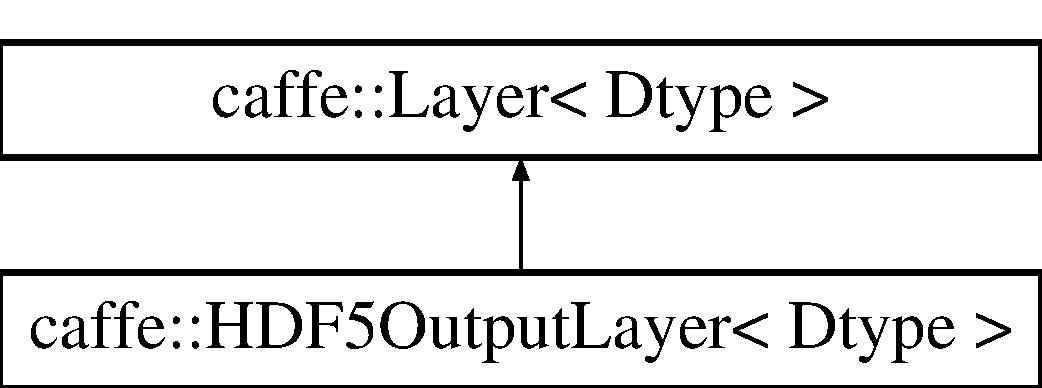
\includegraphics[height=2.000000cm]{classcaffe_1_1_h_d_f5_output_layer}
\end{center}
\end{figure}
\subsection*{Public Member Functions}
\begin{DoxyCompactItemize}
\item 
\hyperlink{classcaffe_1_1_h_d_f5_output_layer_acf9e02d15a72cb6838e8fd2860e046b5}{H\+D\+F5\+Output\+Layer} (const Layer\+Parameter \&param)
\item 
virtual \hyperlink{classcaffe_1_1_h_d_f5_output_layer_a10ea92da7b4bd56dd01734ff62048132}{$\sim$\+H\+D\+F5\+Output\+Layer} ()
\item 
virtual void \hyperlink{classcaffe_1_1_h_d_f5_output_layer_ac30de09e62b1ad98c377f48a7c271ee7}{Set\+Up} (const vector$<$ \hyperlink{classcaffe_1_1_blob}{Blob}$<$ Dtype $>$ $\ast$ $>$ \&bottom, vector$<$ \hyperlink{classcaffe_1_1_blob}{Blob}$<$ Dtype $>$ $\ast$ $>$ $\ast$top)
\item 
std\+::string \hyperlink{classcaffe_1_1_h_d_f5_output_layer_aca8e3392384521de35e87618d3208571}{file\+\_\+name} () const 
\end{DoxyCompactItemize}
\subsection*{Protected Member Functions}
\begin{DoxyCompactItemize}
\item 
virtual Dtype \hyperlink{classcaffe_1_1_h_d_f5_output_layer_a91f77d8f66e4de8280e681f9155b20fa}{Forward\+\_\+cpu} (const vector$<$ \hyperlink{classcaffe_1_1_blob}{Blob}$<$ Dtype $>$ $\ast$ $>$ \&bottom, vector$<$ \hyperlink{classcaffe_1_1_blob}{Blob}$<$ Dtype $>$ $\ast$ $>$ $\ast$top)
\item 
virtual Dtype \hyperlink{classcaffe_1_1_h_d_f5_output_layer_a9f78145efc3bb9ecc7d6a78a3e9c3856}{Forward\+\_\+gpu} (const vector$<$ \hyperlink{classcaffe_1_1_blob}{Blob}$<$ Dtype $>$ $\ast$ $>$ \&bottom, vector$<$ \hyperlink{classcaffe_1_1_blob}{Blob}$<$ Dtype $>$ $\ast$ $>$ $\ast$top)
\item 
virtual void \hyperlink{classcaffe_1_1_h_d_f5_output_layer_a805cc611664761d199b5eb54ba20de0c}{Backward\+\_\+cpu} (const vector$<$ \hyperlink{classcaffe_1_1_blob}{Blob}$<$ Dtype $>$ $\ast$ $>$ \&top, const bool propagate\+\_\+down, vector$<$ \hyperlink{classcaffe_1_1_blob}{Blob}$<$ Dtype $>$ $\ast$ $>$ $\ast$bottom)
\item 
virtual void \hyperlink{classcaffe_1_1_h_d_f5_output_layer_a2018b7ab2f08f004bf967b177e1bb724}{Backward\+\_\+gpu} (const vector$<$ \hyperlink{classcaffe_1_1_blob}{Blob}$<$ Dtype $>$ $\ast$ $>$ \&top, const bool propagate\+\_\+down, vector$<$ \hyperlink{classcaffe_1_1_blob}{Blob}$<$ Dtype $>$ $\ast$ $>$ $\ast$bottom)
\item 
virtual void \hyperlink{classcaffe_1_1_h_d_f5_output_layer_a56c7ba8e69d0867d550dddd928863a2f}{Save\+Blobs} ()
\end{DoxyCompactItemize}
\subsection*{Protected Attributes}
\begin{DoxyCompactItemize}
\item 
std\+::string \hyperlink{classcaffe_1_1_h_d_f5_output_layer_aa4609affd7a57ba7481b98afed3f7985}{file\+\_\+name\+\_\+}
\item 
hid\+\_\+t \hyperlink{classcaffe_1_1_h_d_f5_output_layer_a353a5e36b3baa08e381dc5da1bb8b74e}{file\+\_\+id\+\_\+}
\item 
\hyperlink{classcaffe_1_1_blob}{Blob}$<$ Dtype $>$ \hyperlink{classcaffe_1_1_h_d_f5_output_layer_ad91a29d84d4f7c577adf1b634fec1d92}{data\+\_\+blob\+\_\+}
\item 
\hyperlink{classcaffe_1_1_blob}{Blob}$<$ Dtype $>$ \hyperlink{classcaffe_1_1_h_d_f5_output_layer_aef72be0097ab1894a5414b74512e3807}{label\+\_\+blob\+\_\+}
\end{DoxyCompactItemize}


\subsection{Constructor \& Destructor Documentation}
\hypertarget{classcaffe_1_1_h_d_f5_output_layer_acf9e02d15a72cb6838e8fd2860e046b5}{\index{caffe\+::\+H\+D\+F5\+Output\+Layer@{caffe\+::\+H\+D\+F5\+Output\+Layer}!H\+D\+F5\+Output\+Layer@{H\+D\+F5\+Output\+Layer}}
\index{H\+D\+F5\+Output\+Layer@{H\+D\+F5\+Output\+Layer}!caffe\+::\+H\+D\+F5\+Output\+Layer@{caffe\+::\+H\+D\+F5\+Output\+Layer}}
\subsubsection[{H\+D\+F5\+Output\+Layer}]{\setlength{\rightskip}{0pt plus 5cm}template$<$typename Dtype $>$ {\bf caffe\+::\+H\+D\+F5\+Output\+Layer}$<$ Dtype $>$\+::{\bf H\+D\+F5\+Output\+Layer} (
\begin{DoxyParamCaption}
\item[{const Layer\+Parameter \&}]{param}
\end{DoxyParamCaption}
)\hspace{0.3cm}{\ttfamily [explicit]}}}\label{classcaffe_1_1_h_d_f5_output_layer_acf9e02d15a72cb6838e8fd2860e046b5}
\hypertarget{classcaffe_1_1_h_d_f5_output_layer_a10ea92da7b4bd56dd01734ff62048132}{\index{caffe\+::\+H\+D\+F5\+Output\+Layer@{caffe\+::\+H\+D\+F5\+Output\+Layer}!````~H\+D\+F5\+Output\+Layer@{$\sim$\+H\+D\+F5\+Output\+Layer}}
\index{````~H\+D\+F5\+Output\+Layer@{$\sim$\+H\+D\+F5\+Output\+Layer}!caffe\+::\+H\+D\+F5\+Output\+Layer@{caffe\+::\+H\+D\+F5\+Output\+Layer}}
\subsubsection[{$\sim$\+H\+D\+F5\+Output\+Layer}]{\setlength{\rightskip}{0pt plus 5cm}template$<$typename Dtype $>$ {\bf caffe\+::\+H\+D\+F5\+Output\+Layer}$<$ Dtype $>$\+::$\sim${\bf H\+D\+F5\+Output\+Layer}$<$ Dtype $>$ (
\begin{DoxyParamCaption}
{}
\end{DoxyParamCaption}
)\hspace{0.3cm}{\ttfamily [virtual]}}}\label{classcaffe_1_1_h_d_f5_output_layer_a10ea92da7b4bd56dd01734ff62048132}


\subsection{Member Function Documentation}
\hypertarget{classcaffe_1_1_h_d_f5_output_layer_a805cc611664761d199b5eb54ba20de0c}{\index{caffe\+::\+H\+D\+F5\+Output\+Layer@{caffe\+::\+H\+D\+F5\+Output\+Layer}!Backward\+\_\+cpu@{Backward\+\_\+cpu}}
\index{Backward\+\_\+cpu@{Backward\+\_\+cpu}!caffe\+::\+H\+D\+F5\+Output\+Layer@{caffe\+::\+H\+D\+F5\+Output\+Layer}}
\subsubsection[{Backward\+\_\+cpu}]{\setlength{\rightskip}{0pt plus 5cm}template$<$typename Dtype $>$ void {\bf caffe\+::\+H\+D\+F5\+Output\+Layer}$<$ Dtype $>$\+::Backward\+\_\+cpu (
\begin{DoxyParamCaption}
\item[{const vector$<$ {\bf Blob}$<$ Dtype $>$ $\ast$ $>$ \&}]{top, }
\item[{const bool}]{propagate\+\_\+down, }
\item[{vector$<$ {\bf Blob}$<$ Dtype $>$ $\ast$ $>$ $\ast$}]{bottom}
\end{DoxyParamCaption}
)\hspace{0.3cm}{\ttfamily [protected]}, {\ttfamily [virtual]}}}\label{classcaffe_1_1_h_d_f5_output_layer_a805cc611664761d199b5eb54ba20de0c}


Implements \hyperlink{classcaffe_1_1_layer_ac2d82011d076237c67997f63e7ee4b80}{caffe\+::\+Layer$<$ Dtype $>$}.

\hypertarget{classcaffe_1_1_h_d_f5_output_layer_a2018b7ab2f08f004bf967b177e1bb724}{\index{caffe\+::\+H\+D\+F5\+Output\+Layer@{caffe\+::\+H\+D\+F5\+Output\+Layer}!Backward\+\_\+gpu@{Backward\+\_\+gpu}}
\index{Backward\+\_\+gpu@{Backward\+\_\+gpu}!caffe\+::\+H\+D\+F5\+Output\+Layer@{caffe\+::\+H\+D\+F5\+Output\+Layer}}
\subsubsection[{Backward\+\_\+gpu}]{\setlength{\rightskip}{0pt plus 5cm}template$<$typename Dtype $>$ void {\bf caffe\+::\+H\+D\+F5\+Output\+Layer}$<$ Dtype $>$\+::Backward\+\_\+gpu (
\begin{DoxyParamCaption}
\item[{const vector$<$ {\bf Blob}$<$ Dtype $>$ $\ast$ $>$ \&}]{top, }
\item[{const bool}]{propagate\+\_\+down, }
\item[{vector$<$ {\bf Blob}$<$ Dtype $>$ $\ast$ $>$ $\ast$}]{bottom}
\end{DoxyParamCaption}
)\hspace{0.3cm}{\ttfamily [protected]}, {\ttfamily [virtual]}}}\label{classcaffe_1_1_h_d_f5_output_layer_a2018b7ab2f08f004bf967b177e1bb724}


Reimplemented from \hyperlink{classcaffe_1_1_layer_adf07ffe1f22d2fd2b1b0ff475ef5a64b}{caffe\+::\+Layer$<$ Dtype $>$}.

\hypertarget{classcaffe_1_1_h_d_f5_output_layer_aca8e3392384521de35e87618d3208571}{\index{caffe\+::\+H\+D\+F5\+Output\+Layer@{caffe\+::\+H\+D\+F5\+Output\+Layer}!file\+\_\+name@{file\+\_\+name}}
\index{file\+\_\+name@{file\+\_\+name}!caffe\+::\+H\+D\+F5\+Output\+Layer@{caffe\+::\+H\+D\+F5\+Output\+Layer}}
\subsubsection[{file\+\_\+name}]{\setlength{\rightskip}{0pt plus 5cm}template$<$typename Dtype $>$ std\+::string {\bf caffe\+::\+H\+D\+F5\+Output\+Layer}$<$ Dtype $>$\+::file\+\_\+name (
\begin{DoxyParamCaption}
{}
\end{DoxyParamCaption}
) const\hspace{0.3cm}{\ttfamily [inline]}}}\label{classcaffe_1_1_h_d_f5_output_layer_aca8e3392384521de35e87618d3208571}
\hypertarget{classcaffe_1_1_h_d_f5_output_layer_a91f77d8f66e4de8280e681f9155b20fa}{\index{caffe\+::\+H\+D\+F5\+Output\+Layer@{caffe\+::\+H\+D\+F5\+Output\+Layer}!Forward\+\_\+cpu@{Forward\+\_\+cpu}}
\index{Forward\+\_\+cpu@{Forward\+\_\+cpu}!caffe\+::\+H\+D\+F5\+Output\+Layer@{caffe\+::\+H\+D\+F5\+Output\+Layer}}
\subsubsection[{Forward\+\_\+cpu}]{\setlength{\rightskip}{0pt plus 5cm}template$<$typename Dtype $>$ Dtype {\bf caffe\+::\+H\+D\+F5\+Output\+Layer}$<$ Dtype $>$\+::Forward\+\_\+cpu (
\begin{DoxyParamCaption}
\item[{const vector$<$ {\bf Blob}$<$ Dtype $>$ $\ast$ $>$ \&}]{bottom, }
\item[{vector$<$ {\bf Blob}$<$ Dtype $>$ $\ast$ $>$ $\ast$}]{top}
\end{DoxyParamCaption}
)\hspace{0.3cm}{\ttfamily [protected]}, {\ttfamily [virtual]}}}\label{classcaffe_1_1_h_d_f5_output_layer_a91f77d8f66e4de8280e681f9155b20fa}


Implements \hyperlink{classcaffe_1_1_layer_a8f7f61da3b8b3ca7f2394dee33873353}{caffe\+::\+Layer$<$ Dtype $>$}.

\hypertarget{classcaffe_1_1_h_d_f5_output_layer_a9f78145efc3bb9ecc7d6a78a3e9c3856}{\index{caffe\+::\+H\+D\+F5\+Output\+Layer@{caffe\+::\+H\+D\+F5\+Output\+Layer}!Forward\+\_\+gpu@{Forward\+\_\+gpu}}
\index{Forward\+\_\+gpu@{Forward\+\_\+gpu}!caffe\+::\+H\+D\+F5\+Output\+Layer@{caffe\+::\+H\+D\+F5\+Output\+Layer}}
\subsubsection[{Forward\+\_\+gpu}]{\setlength{\rightskip}{0pt plus 5cm}template$<$typename Dtype $>$ Dtype {\bf caffe\+::\+H\+D\+F5\+Output\+Layer}$<$ Dtype $>$\+::Forward\+\_\+gpu (
\begin{DoxyParamCaption}
\item[{const vector$<$ {\bf Blob}$<$ Dtype $>$ $\ast$ $>$ \&}]{bottom, }
\item[{vector$<$ {\bf Blob}$<$ Dtype $>$ $\ast$ $>$ $\ast$}]{top}
\end{DoxyParamCaption}
)\hspace{0.3cm}{\ttfamily [protected]}, {\ttfamily [virtual]}}}\label{classcaffe_1_1_h_d_f5_output_layer_a9f78145efc3bb9ecc7d6a78a3e9c3856}


Reimplemented from \hyperlink{classcaffe_1_1_layer_a2d78dbf5d8bc36928bd8f6fcfbafbcef}{caffe\+::\+Layer$<$ Dtype $>$}.

\hypertarget{classcaffe_1_1_h_d_f5_output_layer_a56c7ba8e69d0867d550dddd928863a2f}{\index{caffe\+::\+H\+D\+F5\+Output\+Layer@{caffe\+::\+H\+D\+F5\+Output\+Layer}!Save\+Blobs@{Save\+Blobs}}
\index{Save\+Blobs@{Save\+Blobs}!caffe\+::\+H\+D\+F5\+Output\+Layer@{caffe\+::\+H\+D\+F5\+Output\+Layer}}
\subsubsection[{Save\+Blobs}]{\setlength{\rightskip}{0pt plus 5cm}template$<$typename Dtype $>$ void {\bf caffe\+::\+H\+D\+F5\+Output\+Layer}$<$ Dtype $>$\+::Save\+Blobs (
\begin{DoxyParamCaption}
{}
\end{DoxyParamCaption}
)\hspace{0.3cm}{\ttfamily [protected]}, {\ttfamily [virtual]}}}\label{classcaffe_1_1_h_d_f5_output_layer_a56c7ba8e69d0867d550dddd928863a2f}
\hypertarget{classcaffe_1_1_h_d_f5_output_layer_ac30de09e62b1ad98c377f48a7c271ee7}{\index{caffe\+::\+H\+D\+F5\+Output\+Layer@{caffe\+::\+H\+D\+F5\+Output\+Layer}!Set\+Up@{Set\+Up}}
\index{Set\+Up@{Set\+Up}!caffe\+::\+H\+D\+F5\+Output\+Layer@{caffe\+::\+H\+D\+F5\+Output\+Layer}}
\subsubsection[{Set\+Up}]{\setlength{\rightskip}{0pt plus 5cm}template$<$typename Dtype $>$ void {\bf caffe\+::\+H\+D\+F5\+Output\+Layer}$<$ Dtype $>$\+::Set\+Up (
\begin{DoxyParamCaption}
\item[{const vector$<$ {\bf Blob}$<$ Dtype $>$ $\ast$ $>$ \&}]{bottom, }
\item[{vector$<$ {\bf Blob}$<$ Dtype $>$ $\ast$ $>$ $\ast$}]{top}
\end{DoxyParamCaption}
)\hspace{0.3cm}{\ttfamily [virtual]}}}\label{classcaffe_1_1_h_d_f5_output_layer_ac30de09e62b1ad98c377f48a7c271ee7}


Implements \hyperlink{classcaffe_1_1_layer_abd13c6489c13953b4fbcfcf6880835d0}{caffe\+::\+Layer$<$ Dtype $>$}.



\subsection{Member Data Documentation}
\hypertarget{classcaffe_1_1_h_d_f5_output_layer_ad91a29d84d4f7c577adf1b634fec1d92}{\index{caffe\+::\+H\+D\+F5\+Output\+Layer@{caffe\+::\+H\+D\+F5\+Output\+Layer}!data\+\_\+blob\+\_\+@{data\+\_\+blob\+\_\+}}
\index{data\+\_\+blob\+\_\+@{data\+\_\+blob\+\_\+}!caffe\+::\+H\+D\+F5\+Output\+Layer@{caffe\+::\+H\+D\+F5\+Output\+Layer}}
\subsubsection[{data\+\_\+blob\+\_\+}]{\setlength{\rightskip}{0pt plus 5cm}template$<$typename Dtype $>$ {\bf Blob}$<$Dtype$>$ {\bf caffe\+::\+H\+D\+F5\+Output\+Layer}$<$ Dtype $>$\+::data\+\_\+blob\+\_\+\hspace{0.3cm}{\ttfamily [protected]}}}\label{classcaffe_1_1_h_d_f5_output_layer_ad91a29d84d4f7c577adf1b634fec1d92}
\hypertarget{classcaffe_1_1_h_d_f5_output_layer_a353a5e36b3baa08e381dc5da1bb8b74e}{\index{caffe\+::\+H\+D\+F5\+Output\+Layer@{caffe\+::\+H\+D\+F5\+Output\+Layer}!file\+\_\+id\+\_\+@{file\+\_\+id\+\_\+}}
\index{file\+\_\+id\+\_\+@{file\+\_\+id\+\_\+}!caffe\+::\+H\+D\+F5\+Output\+Layer@{caffe\+::\+H\+D\+F5\+Output\+Layer}}
\subsubsection[{file\+\_\+id\+\_\+}]{\setlength{\rightskip}{0pt plus 5cm}template$<$typename Dtype $>$ hid\+\_\+t {\bf caffe\+::\+H\+D\+F5\+Output\+Layer}$<$ Dtype $>$\+::file\+\_\+id\+\_\+\hspace{0.3cm}{\ttfamily [protected]}}}\label{classcaffe_1_1_h_d_f5_output_layer_a353a5e36b3baa08e381dc5da1bb8b74e}
\hypertarget{classcaffe_1_1_h_d_f5_output_layer_aa4609affd7a57ba7481b98afed3f7985}{\index{caffe\+::\+H\+D\+F5\+Output\+Layer@{caffe\+::\+H\+D\+F5\+Output\+Layer}!file\+\_\+name\+\_\+@{file\+\_\+name\+\_\+}}
\index{file\+\_\+name\+\_\+@{file\+\_\+name\+\_\+}!caffe\+::\+H\+D\+F5\+Output\+Layer@{caffe\+::\+H\+D\+F5\+Output\+Layer}}
\subsubsection[{file\+\_\+name\+\_\+}]{\setlength{\rightskip}{0pt plus 5cm}template$<$typename Dtype $>$ std\+::string {\bf caffe\+::\+H\+D\+F5\+Output\+Layer}$<$ Dtype $>$\+::file\+\_\+name\+\_\+\hspace{0.3cm}{\ttfamily [protected]}}}\label{classcaffe_1_1_h_d_f5_output_layer_aa4609affd7a57ba7481b98afed3f7985}
\hypertarget{classcaffe_1_1_h_d_f5_output_layer_aef72be0097ab1894a5414b74512e3807}{\index{caffe\+::\+H\+D\+F5\+Output\+Layer@{caffe\+::\+H\+D\+F5\+Output\+Layer}!label\+\_\+blob\+\_\+@{label\+\_\+blob\+\_\+}}
\index{label\+\_\+blob\+\_\+@{label\+\_\+blob\+\_\+}!caffe\+::\+H\+D\+F5\+Output\+Layer@{caffe\+::\+H\+D\+F5\+Output\+Layer}}
\subsubsection[{label\+\_\+blob\+\_\+}]{\setlength{\rightskip}{0pt plus 5cm}template$<$typename Dtype $>$ {\bf Blob}$<$Dtype$>$ {\bf caffe\+::\+H\+D\+F5\+Output\+Layer}$<$ Dtype $>$\+::label\+\_\+blob\+\_\+\hspace{0.3cm}{\ttfamily [protected]}}}\label{classcaffe_1_1_h_d_f5_output_layer_aef72be0097ab1894a5414b74512e3807}


The documentation for this class was generated from the following files\+:\begin{DoxyCompactItemize}
\item 
include/caffe/\hyperlink{vision__layers_8hpp}{vision\+\_\+layers.\+hpp}\item 
src/caffe/layers/\hyperlink{hdf5__output__layer_8cpp}{hdf5\+\_\+output\+\_\+layer.\+cpp}\item 
src/caffe/layers/\hyperlink{hdf5__output__layer_8cu}{hdf5\+\_\+output\+\_\+layer.\+cu}\end{DoxyCompactItemize}

\hypertarget{classcaffe_1_1_h_d_f5_output_layer_test}{\section{caffe\+:\+:H\+D\+F5\+Output\+Layer\+Test$<$ Dtype $>$ Class Template Reference}
\label{classcaffe_1_1_h_d_f5_output_layer_test}\index{caffe\+::\+H\+D\+F5\+Output\+Layer\+Test$<$ Dtype $>$@{caffe\+::\+H\+D\+F5\+Output\+Layer\+Test$<$ Dtype $>$}}
}
Inheritance diagram for caffe\+:\+:H\+D\+F5\+Output\+Layer\+Test$<$ Dtype $>$\+:\begin{figure}[H]
\begin{center}
\leavevmode
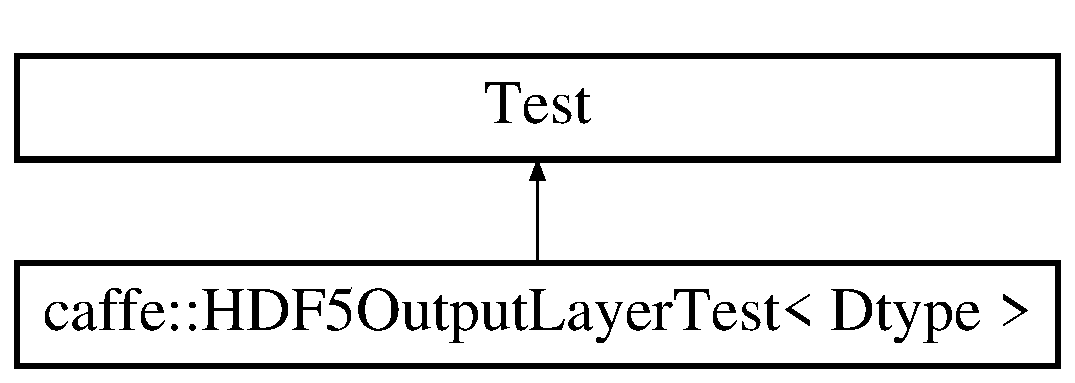
\includegraphics[height=2.000000cm]{classcaffe_1_1_h_d_f5_output_layer_test}
\end{center}
\end{figure}
\subsection*{Protected Member Functions}
\begin{DoxyCompactItemize}
\item 
\hyperlink{classcaffe_1_1_h_d_f5_output_layer_test_acee50633466c0b51ac035ddf36aa0cce}{H\+D\+F5\+Output\+Layer\+Test} ()
\item 
virtual \hyperlink{classcaffe_1_1_h_d_f5_output_layer_test_a371fac84fea6914e6fe5a0706628f700}{$\sim$\+H\+D\+F5\+Output\+Layer\+Test} ()
\item 
void \hyperlink{classcaffe_1_1_h_d_f5_output_layer_test_a8b5a19f721a52d532cc4118b2302e450}{Check\+Blob\+Equal} (const \hyperlink{classcaffe_1_1_blob}{Blob}$<$ Dtype $>$ \&b1, const \hyperlink{classcaffe_1_1_blob}{Blob}$<$ Dtype $>$ \&b2)
\end{DoxyCompactItemize}
\subsection*{Protected Attributes}
\begin{DoxyCompactItemize}
\item 
string \hyperlink{classcaffe_1_1_h_d_f5_output_layer_test_a5ba970f78ba51ce6362c6e3a1245e9ad}{output\+\_\+file\+\_\+name\+\_\+}
\item 
string \hyperlink{classcaffe_1_1_h_d_f5_output_layer_test_a0174a018fc1542aa473d53e406c37288}{input\+\_\+file\+\_\+name\+\_\+}
\item 
\hyperlink{classcaffe_1_1_blob}{Blob}$<$ Dtype $>$ $\ast$const \hyperlink{classcaffe_1_1_h_d_f5_output_layer_test_a68d23919519dc2fccf5f851dc67bb03e}{blob\+\_\+data\+\_\+}
\item 
\hyperlink{classcaffe_1_1_blob}{Blob}$<$ Dtype $>$ $\ast$const \hyperlink{classcaffe_1_1_h_d_f5_output_layer_test_aa87f34a2f1fed9e69cebe794fef7e1fb}{blob\+\_\+label\+\_\+}
\item 
vector$<$ \hyperlink{classcaffe_1_1_blob}{Blob}$<$ Dtype $>$ $\ast$ $>$ \hyperlink{classcaffe_1_1_h_d_f5_output_layer_test_a954c71b6deb34d3c68f41e74a98cb707}{blob\+\_\+bottom\+\_\+vec\+\_\+}
\item 
vector$<$ \hyperlink{classcaffe_1_1_blob}{Blob}$<$ Dtype $>$ $\ast$ $>$ \hyperlink{classcaffe_1_1_h_d_f5_output_layer_test_a7d062445759c5dc03e94de9e78794311}{blob\+\_\+top\+\_\+vec\+\_\+}
\item 
int \hyperlink{classcaffe_1_1_h_d_f5_output_layer_test_a7a7fca0de69992efdaef17f80a47b373}{num\+\_\+}
\item 
int \hyperlink{classcaffe_1_1_h_d_f5_output_layer_test_a08738f3c6c8b50d963684e9b036f1402}{channels\+\_\+}
\item 
int \hyperlink{classcaffe_1_1_h_d_f5_output_layer_test_a542fea46c7211a5e74aa414291414e0d}{height\+\_\+}
\item 
int \hyperlink{classcaffe_1_1_h_d_f5_output_layer_test_a867e7d0a5fc961566ed6be297f292401}{width\+\_\+}
\end{DoxyCompactItemize}


\subsection{Constructor \& Destructor Documentation}
\hypertarget{classcaffe_1_1_h_d_f5_output_layer_test_acee50633466c0b51ac035ddf36aa0cce}{\index{caffe\+::\+H\+D\+F5\+Output\+Layer\+Test@{caffe\+::\+H\+D\+F5\+Output\+Layer\+Test}!H\+D\+F5\+Output\+Layer\+Test@{H\+D\+F5\+Output\+Layer\+Test}}
\index{H\+D\+F5\+Output\+Layer\+Test@{H\+D\+F5\+Output\+Layer\+Test}!caffe\+::\+H\+D\+F5\+Output\+Layer\+Test@{caffe\+::\+H\+D\+F5\+Output\+Layer\+Test}}
\subsubsection[{H\+D\+F5\+Output\+Layer\+Test}]{\setlength{\rightskip}{0pt plus 5cm}template$<$typename Dtype $>$ {\bf caffe\+::\+H\+D\+F5\+Output\+Layer\+Test}$<$ Dtype $>$\+::{\bf H\+D\+F5\+Output\+Layer\+Test} (
\begin{DoxyParamCaption}
{}
\end{DoxyParamCaption}
)\hspace{0.3cm}{\ttfamily [inline]}, {\ttfamily [protected]}}}\label{classcaffe_1_1_h_d_f5_output_layer_test_acee50633466c0b51ac035ddf36aa0cce}
\hypertarget{classcaffe_1_1_h_d_f5_output_layer_test_a371fac84fea6914e6fe5a0706628f700}{\index{caffe\+::\+H\+D\+F5\+Output\+Layer\+Test@{caffe\+::\+H\+D\+F5\+Output\+Layer\+Test}!````~H\+D\+F5\+Output\+Layer\+Test@{$\sim$\+H\+D\+F5\+Output\+Layer\+Test}}
\index{````~H\+D\+F5\+Output\+Layer\+Test@{$\sim$\+H\+D\+F5\+Output\+Layer\+Test}!caffe\+::\+H\+D\+F5\+Output\+Layer\+Test@{caffe\+::\+H\+D\+F5\+Output\+Layer\+Test}}
\subsubsection[{$\sim$\+H\+D\+F5\+Output\+Layer\+Test}]{\setlength{\rightskip}{0pt plus 5cm}template$<$typename Dtype $>$ virtual {\bf caffe\+::\+H\+D\+F5\+Output\+Layer\+Test}$<$ Dtype $>$\+::$\sim${\bf H\+D\+F5\+Output\+Layer\+Test} (
\begin{DoxyParamCaption}
{}
\end{DoxyParamCaption}
)\hspace{0.3cm}{\ttfamily [inline]}, {\ttfamily [protected]}, {\ttfamily [virtual]}}}\label{classcaffe_1_1_h_d_f5_output_layer_test_a371fac84fea6914e6fe5a0706628f700}


\subsection{Member Function Documentation}
\hypertarget{classcaffe_1_1_h_d_f5_output_layer_test_a8b5a19f721a52d532cc4118b2302e450}{\index{caffe\+::\+H\+D\+F5\+Output\+Layer\+Test@{caffe\+::\+H\+D\+F5\+Output\+Layer\+Test}!Check\+Blob\+Equal@{Check\+Blob\+Equal}}
\index{Check\+Blob\+Equal@{Check\+Blob\+Equal}!caffe\+::\+H\+D\+F5\+Output\+Layer\+Test@{caffe\+::\+H\+D\+F5\+Output\+Layer\+Test}}
\subsubsection[{Check\+Blob\+Equal}]{\setlength{\rightskip}{0pt plus 5cm}template$<$typename Dtype $>$ void {\bf caffe\+::\+H\+D\+F5\+Output\+Layer\+Test}$<$ Dtype $>$\+::Check\+Blob\+Equal (
\begin{DoxyParamCaption}
\item[{const {\bf Blob}$<$ Dtype $>$ \&}]{b1, }
\item[{const {\bf Blob}$<$ Dtype $>$ \&}]{b2}
\end{DoxyParamCaption}
)\hspace{0.3cm}{\ttfamily [protected]}}}\label{classcaffe_1_1_h_d_f5_output_layer_test_a8b5a19f721a52d532cc4118b2302e450}


\subsection{Member Data Documentation}
\hypertarget{classcaffe_1_1_h_d_f5_output_layer_test_a954c71b6deb34d3c68f41e74a98cb707}{\index{caffe\+::\+H\+D\+F5\+Output\+Layer\+Test@{caffe\+::\+H\+D\+F5\+Output\+Layer\+Test}!blob\+\_\+bottom\+\_\+vec\+\_\+@{blob\+\_\+bottom\+\_\+vec\+\_\+}}
\index{blob\+\_\+bottom\+\_\+vec\+\_\+@{blob\+\_\+bottom\+\_\+vec\+\_\+}!caffe\+::\+H\+D\+F5\+Output\+Layer\+Test@{caffe\+::\+H\+D\+F5\+Output\+Layer\+Test}}
\subsubsection[{blob\+\_\+bottom\+\_\+vec\+\_\+}]{\setlength{\rightskip}{0pt plus 5cm}template$<$typename Dtype $>$ vector$<${\bf Blob}$<$Dtype$>$$\ast$$>$ {\bf caffe\+::\+H\+D\+F5\+Output\+Layer\+Test}$<$ Dtype $>$\+::blob\+\_\+bottom\+\_\+vec\+\_\+\hspace{0.3cm}{\ttfamily [protected]}}}\label{classcaffe_1_1_h_d_f5_output_layer_test_a954c71b6deb34d3c68f41e74a98cb707}
\hypertarget{classcaffe_1_1_h_d_f5_output_layer_test_a68d23919519dc2fccf5f851dc67bb03e}{\index{caffe\+::\+H\+D\+F5\+Output\+Layer\+Test@{caffe\+::\+H\+D\+F5\+Output\+Layer\+Test}!blob\+\_\+data\+\_\+@{blob\+\_\+data\+\_\+}}
\index{blob\+\_\+data\+\_\+@{blob\+\_\+data\+\_\+}!caffe\+::\+H\+D\+F5\+Output\+Layer\+Test@{caffe\+::\+H\+D\+F5\+Output\+Layer\+Test}}
\subsubsection[{blob\+\_\+data\+\_\+}]{\setlength{\rightskip}{0pt plus 5cm}template$<$typename Dtype $>$ {\bf Blob}$<$Dtype$>$$\ast$ const {\bf caffe\+::\+H\+D\+F5\+Output\+Layer\+Test}$<$ Dtype $>$\+::blob\+\_\+data\+\_\+\hspace{0.3cm}{\ttfamily [protected]}}}\label{classcaffe_1_1_h_d_f5_output_layer_test_a68d23919519dc2fccf5f851dc67bb03e}
\hypertarget{classcaffe_1_1_h_d_f5_output_layer_test_aa87f34a2f1fed9e69cebe794fef7e1fb}{\index{caffe\+::\+H\+D\+F5\+Output\+Layer\+Test@{caffe\+::\+H\+D\+F5\+Output\+Layer\+Test}!blob\+\_\+label\+\_\+@{blob\+\_\+label\+\_\+}}
\index{blob\+\_\+label\+\_\+@{blob\+\_\+label\+\_\+}!caffe\+::\+H\+D\+F5\+Output\+Layer\+Test@{caffe\+::\+H\+D\+F5\+Output\+Layer\+Test}}
\subsubsection[{blob\+\_\+label\+\_\+}]{\setlength{\rightskip}{0pt plus 5cm}template$<$typename Dtype $>$ {\bf Blob}$<$Dtype$>$$\ast$ const {\bf caffe\+::\+H\+D\+F5\+Output\+Layer\+Test}$<$ Dtype $>$\+::blob\+\_\+label\+\_\+\hspace{0.3cm}{\ttfamily [protected]}}}\label{classcaffe_1_1_h_d_f5_output_layer_test_aa87f34a2f1fed9e69cebe794fef7e1fb}
\hypertarget{classcaffe_1_1_h_d_f5_output_layer_test_a7d062445759c5dc03e94de9e78794311}{\index{caffe\+::\+H\+D\+F5\+Output\+Layer\+Test@{caffe\+::\+H\+D\+F5\+Output\+Layer\+Test}!blob\+\_\+top\+\_\+vec\+\_\+@{blob\+\_\+top\+\_\+vec\+\_\+}}
\index{blob\+\_\+top\+\_\+vec\+\_\+@{blob\+\_\+top\+\_\+vec\+\_\+}!caffe\+::\+H\+D\+F5\+Output\+Layer\+Test@{caffe\+::\+H\+D\+F5\+Output\+Layer\+Test}}
\subsubsection[{blob\+\_\+top\+\_\+vec\+\_\+}]{\setlength{\rightskip}{0pt plus 5cm}template$<$typename Dtype $>$ vector$<${\bf Blob}$<$Dtype$>$$\ast$$>$ {\bf caffe\+::\+H\+D\+F5\+Output\+Layer\+Test}$<$ Dtype $>$\+::blob\+\_\+top\+\_\+vec\+\_\+\hspace{0.3cm}{\ttfamily [protected]}}}\label{classcaffe_1_1_h_d_f5_output_layer_test_a7d062445759c5dc03e94de9e78794311}
\hypertarget{classcaffe_1_1_h_d_f5_output_layer_test_a08738f3c6c8b50d963684e9b036f1402}{\index{caffe\+::\+H\+D\+F5\+Output\+Layer\+Test@{caffe\+::\+H\+D\+F5\+Output\+Layer\+Test}!channels\+\_\+@{channels\+\_\+}}
\index{channels\+\_\+@{channels\+\_\+}!caffe\+::\+H\+D\+F5\+Output\+Layer\+Test@{caffe\+::\+H\+D\+F5\+Output\+Layer\+Test}}
\subsubsection[{channels\+\_\+}]{\setlength{\rightskip}{0pt plus 5cm}template$<$typename Dtype $>$ int {\bf caffe\+::\+H\+D\+F5\+Output\+Layer\+Test}$<$ Dtype $>$\+::channels\+\_\+\hspace{0.3cm}{\ttfamily [protected]}}}\label{classcaffe_1_1_h_d_f5_output_layer_test_a08738f3c6c8b50d963684e9b036f1402}
\hypertarget{classcaffe_1_1_h_d_f5_output_layer_test_a542fea46c7211a5e74aa414291414e0d}{\index{caffe\+::\+H\+D\+F5\+Output\+Layer\+Test@{caffe\+::\+H\+D\+F5\+Output\+Layer\+Test}!height\+\_\+@{height\+\_\+}}
\index{height\+\_\+@{height\+\_\+}!caffe\+::\+H\+D\+F5\+Output\+Layer\+Test@{caffe\+::\+H\+D\+F5\+Output\+Layer\+Test}}
\subsubsection[{height\+\_\+}]{\setlength{\rightskip}{0pt plus 5cm}template$<$typename Dtype $>$ int {\bf caffe\+::\+H\+D\+F5\+Output\+Layer\+Test}$<$ Dtype $>$\+::height\+\_\+\hspace{0.3cm}{\ttfamily [protected]}}}\label{classcaffe_1_1_h_d_f5_output_layer_test_a542fea46c7211a5e74aa414291414e0d}
\hypertarget{classcaffe_1_1_h_d_f5_output_layer_test_a0174a018fc1542aa473d53e406c37288}{\index{caffe\+::\+H\+D\+F5\+Output\+Layer\+Test@{caffe\+::\+H\+D\+F5\+Output\+Layer\+Test}!input\+\_\+file\+\_\+name\+\_\+@{input\+\_\+file\+\_\+name\+\_\+}}
\index{input\+\_\+file\+\_\+name\+\_\+@{input\+\_\+file\+\_\+name\+\_\+}!caffe\+::\+H\+D\+F5\+Output\+Layer\+Test@{caffe\+::\+H\+D\+F5\+Output\+Layer\+Test}}
\subsubsection[{input\+\_\+file\+\_\+name\+\_\+}]{\setlength{\rightskip}{0pt plus 5cm}template$<$typename Dtype $>$ string {\bf caffe\+::\+H\+D\+F5\+Output\+Layer\+Test}$<$ Dtype $>$\+::input\+\_\+file\+\_\+name\+\_\+\hspace{0.3cm}{\ttfamily [protected]}}}\label{classcaffe_1_1_h_d_f5_output_layer_test_a0174a018fc1542aa473d53e406c37288}
\hypertarget{classcaffe_1_1_h_d_f5_output_layer_test_a7a7fca0de69992efdaef17f80a47b373}{\index{caffe\+::\+H\+D\+F5\+Output\+Layer\+Test@{caffe\+::\+H\+D\+F5\+Output\+Layer\+Test}!num\+\_\+@{num\+\_\+}}
\index{num\+\_\+@{num\+\_\+}!caffe\+::\+H\+D\+F5\+Output\+Layer\+Test@{caffe\+::\+H\+D\+F5\+Output\+Layer\+Test}}
\subsubsection[{num\+\_\+}]{\setlength{\rightskip}{0pt plus 5cm}template$<$typename Dtype $>$ int {\bf caffe\+::\+H\+D\+F5\+Output\+Layer\+Test}$<$ Dtype $>$\+::num\+\_\+\hspace{0.3cm}{\ttfamily [protected]}}}\label{classcaffe_1_1_h_d_f5_output_layer_test_a7a7fca0de69992efdaef17f80a47b373}
\hypertarget{classcaffe_1_1_h_d_f5_output_layer_test_a5ba970f78ba51ce6362c6e3a1245e9ad}{\index{caffe\+::\+H\+D\+F5\+Output\+Layer\+Test@{caffe\+::\+H\+D\+F5\+Output\+Layer\+Test}!output\+\_\+file\+\_\+name\+\_\+@{output\+\_\+file\+\_\+name\+\_\+}}
\index{output\+\_\+file\+\_\+name\+\_\+@{output\+\_\+file\+\_\+name\+\_\+}!caffe\+::\+H\+D\+F5\+Output\+Layer\+Test@{caffe\+::\+H\+D\+F5\+Output\+Layer\+Test}}
\subsubsection[{output\+\_\+file\+\_\+name\+\_\+}]{\setlength{\rightskip}{0pt plus 5cm}template$<$typename Dtype $>$ string {\bf caffe\+::\+H\+D\+F5\+Output\+Layer\+Test}$<$ Dtype $>$\+::output\+\_\+file\+\_\+name\+\_\+\hspace{0.3cm}{\ttfamily [protected]}}}\label{classcaffe_1_1_h_d_f5_output_layer_test_a5ba970f78ba51ce6362c6e3a1245e9ad}
\hypertarget{classcaffe_1_1_h_d_f5_output_layer_test_a867e7d0a5fc961566ed6be297f292401}{\index{caffe\+::\+H\+D\+F5\+Output\+Layer\+Test@{caffe\+::\+H\+D\+F5\+Output\+Layer\+Test}!width\+\_\+@{width\+\_\+}}
\index{width\+\_\+@{width\+\_\+}!caffe\+::\+H\+D\+F5\+Output\+Layer\+Test@{caffe\+::\+H\+D\+F5\+Output\+Layer\+Test}}
\subsubsection[{width\+\_\+}]{\setlength{\rightskip}{0pt plus 5cm}template$<$typename Dtype $>$ int {\bf caffe\+::\+H\+D\+F5\+Output\+Layer\+Test}$<$ Dtype $>$\+::width\+\_\+\hspace{0.3cm}{\ttfamily [protected]}}}\label{classcaffe_1_1_h_d_f5_output_layer_test_a867e7d0a5fc961566ed6be297f292401}


The documentation for this class was generated from the following file\+:\begin{DoxyCompactItemize}
\item 
src/caffe/test/\hyperlink{test__hdf5__output__layer_8cpp}{test\+\_\+hdf5\+\_\+output\+\_\+layer.\+cpp}\end{DoxyCompactItemize}

\hypertarget{classcaffe_1_1_hinge_loss_layer}{\section{caffe\+:\+:Hinge\+Loss\+Layer$<$ Dtype $>$ Class Template Reference}
\label{classcaffe_1_1_hinge_loss_layer}\index{caffe\+::\+Hinge\+Loss\+Layer$<$ Dtype $>$@{caffe\+::\+Hinge\+Loss\+Layer$<$ Dtype $>$}}
}


{\ttfamily \#include $<$vision\+\_\+layers.\+hpp$>$}

Inheritance diagram for caffe\+:\+:Hinge\+Loss\+Layer$<$ Dtype $>$\+:\begin{figure}[H]
\begin{center}
\leavevmode
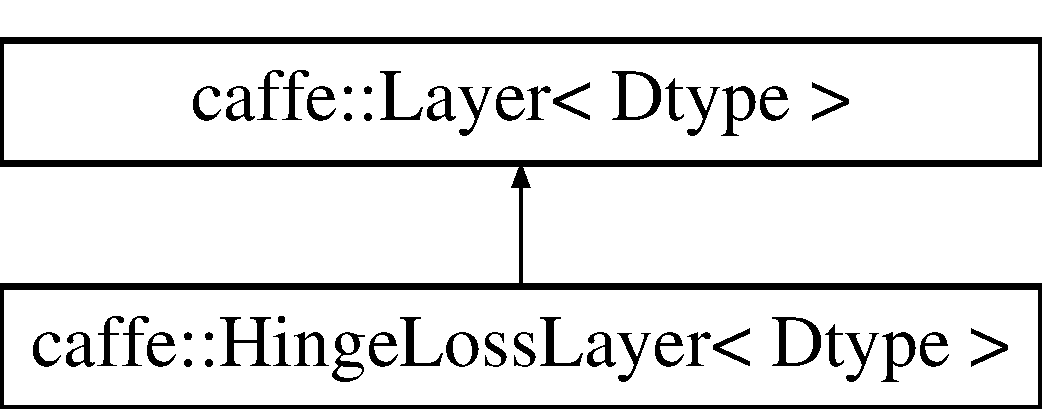
\includegraphics[height=2.000000cm]{classcaffe_1_1_hinge_loss_layer}
\end{center}
\end{figure}
\subsection*{Public Member Functions}
\begin{DoxyCompactItemize}
\item 
\hyperlink{classcaffe_1_1_hinge_loss_layer_a358a5bd2625bb7fed61052dd8e1cb588}{Hinge\+Loss\+Layer} (const Layer\+Parameter \&param)
\item 
virtual void \hyperlink{classcaffe_1_1_hinge_loss_layer_a6674ffab4fc6a97a1545801dad068d42}{Set\+Up} (const vector$<$ \hyperlink{classcaffe_1_1_blob}{Blob}$<$ Dtype $>$ $\ast$ $>$ \&bottom, vector$<$ \hyperlink{classcaffe_1_1_blob}{Blob}$<$ Dtype $>$ $\ast$ $>$ $\ast$top)
\end{DoxyCompactItemize}
\subsection*{Protected Member Functions}
\begin{DoxyCompactItemize}
\item 
virtual Dtype \hyperlink{classcaffe_1_1_hinge_loss_layer_a1e6922952af5ac6989b080ef8cf0c89a}{Forward\+\_\+cpu} (const vector$<$ \hyperlink{classcaffe_1_1_blob}{Blob}$<$ Dtype $>$ $\ast$ $>$ \&bottom, vector$<$ \hyperlink{classcaffe_1_1_blob}{Blob}$<$ Dtype $>$ $\ast$ $>$ $\ast$top)
\item 
virtual void \hyperlink{classcaffe_1_1_hinge_loss_layer_a467c0d92debbaddecf6b18d4bbc31526}{Backward\+\_\+cpu} (const vector$<$ \hyperlink{classcaffe_1_1_blob}{Blob}$<$ Dtype $>$ $\ast$ $>$ \&top, const bool propagate\+\_\+down, vector$<$ \hyperlink{classcaffe_1_1_blob}{Blob}$<$ Dtype $>$ $\ast$ $>$ $\ast$bottom)
\end{DoxyCompactItemize}
\subsection*{Additional Inherited Members}


\subsection{Constructor \& Destructor Documentation}
\hypertarget{classcaffe_1_1_hinge_loss_layer_a358a5bd2625bb7fed61052dd8e1cb588}{\index{caffe\+::\+Hinge\+Loss\+Layer@{caffe\+::\+Hinge\+Loss\+Layer}!Hinge\+Loss\+Layer@{Hinge\+Loss\+Layer}}
\index{Hinge\+Loss\+Layer@{Hinge\+Loss\+Layer}!caffe\+::\+Hinge\+Loss\+Layer@{caffe\+::\+Hinge\+Loss\+Layer}}
\subsubsection[{Hinge\+Loss\+Layer}]{\setlength{\rightskip}{0pt plus 5cm}template$<$typename Dtype $>$ {\bf caffe\+::\+Hinge\+Loss\+Layer}$<$ Dtype $>$\+::{\bf Hinge\+Loss\+Layer} (
\begin{DoxyParamCaption}
\item[{const Layer\+Parameter \&}]{param}
\end{DoxyParamCaption}
)\hspace{0.3cm}{\ttfamily [inline]}, {\ttfamily [explicit]}}}\label{classcaffe_1_1_hinge_loss_layer_a358a5bd2625bb7fed61052dd8e1cb588}


\subsection{Member Function Documentation}
\hypertarget{classcaffe_1_1_hinge_loss_layer_a467c0d92debbaddecf6b18d4bbc31526}{\index{caffe\+::\+Hinge\+Loss\+Layer@{caffe\+::\+Hinge\+Loss\+Layer}!Backward\+\_\+cpu@{Backward\+\_\+cpu}}
\index{Backward\+\_\+cpu@{Backward\+\_\+cpu}!caffe\+::\+Hinge\+Loss\+Layer@{caffe\+::\+Hinge\+Loss\+Layer}}
\subsubsection[{Backward\+\_\+cpu}]{\setlength{\rightskip}{0pt plus 5cm}template$<$typename Dtype $>$ void {\bf caffe\+::\+Hinge\+Loss\+Layer}$<$ Dtype $>$\+::Backward\+\_\+cpu (
\begin{DoxyParamCaption}
\item[{const vector$<$ {\bf Blob}$<$ Dtype $>$ $\ast$ $>$ \&}]{top, }
\item[{const bool}]{propagate\+\_\+down, }
\item[{vector$<$ {\bf Blob}$<$ Dtype $>$ $\ast$ $>$ $\ast$}]{bottom}
\end{DoxyParamCaption}
)\hspace{0.3cm}{\ttfamily [protected]}, {\ttfamily [virtual]}}}\label{classcaffe_1_1_hinge_loss_layer_a467c0d92debbaddecf6b18d4bbc31526}


Implements \hyperlink{classcaffe_1_1_layer_ac2d82011d076237c67997f63e7ee4b80}{caffe\+::\+Layer$<$ Dtype $>$}.

\hypertarget{classcaffe_1_1_hinge_loss_layer_a1e6922952af5ac6989b080ef8cf0c89a}{\index{caffe\+::\+Hinge\+Loss\+Layer@{caffe\+::\+Hinge\+Loss\+Layer}!Forward\+\_\+cpu@{Forward\+\_\+cpu}}
\index{Forward\+\_\+cpu@{Forward\+\_\+cpu}!caffe\+::\+Hinge\+Loss\+Layer@{caffe\+::\+Hinge\+Loss\+Layer}}
\subsubsection[{Forward\+\_\+cpu}]{\setlength{\rightskip}{0pt plus 5cm}template$<$typename Dtype $>$ Dtype {\bf caffe\+::\+Hinge\+Loss\+Layer}$<$ Dtype $>$\+::Forward\+\_\+cpu (
\begin{DoxyParamCaption}
\item[{const vector$<$ {\bf Blob}$<$ Dtype $>$ $\ast$ $>$ \&}]{bottom, }
\item[{vector$<$ {\bf Blob}$<$ Dtype $>$ $\ast$ $>$ $\ast$}]{top}
\end{DoxyParamCaption}
)\hspace{0.3cm}{\ttfamily [protected]}, {\ttfamily [virtual]}}}\label{classcaffe_1_1_hinge_loss_layer_a1e6922952af5ac6989b080ef8cf0c89a}


Implements \hyperlink{classcaffe_1_1_layer_a8f7f61da3b8b3ca7f2394dee33873353}{caffe\+::\+Layer$<$ Dtype $>$}.

\hypertarget{classcaffe_1_1_hinge_loss_layer_a6674ffab4fc6a97a1545801dad068d42}{\index{caffe\+::\+Hinge\+Loss\+Layer@{caffe\+::\+Hinge\+Loss\+Layer}!Set\+Up@{Set\+Up}}
\index{Set\+Up@{Set\+Up}!caffe\+::\+Hinge\+Loss\+Layer@{caffe\+::\+Hinge\+Loss\+Layer}}
\subsubsection[{Set\+Up}]{\setlength{\rightskip}{0pt plus 5cm}template$<$typename Dtype $>$ void {\bf caffe\+::\+Hinge\+Loss\+Layer}$<$ Dtype $>$\+::Set\+Up (
\begin{DoxyParamCaption}
\item[{const vector$<$ {\bf Blob}$<$ Dtype $>$ $\ast$ $>$ \&}]{bottom, }
\item[{vector$<$ {\bf Blob}$<$ Dtype $>$ $\ast$ $>$ $\ast$}]{top}
\end{DoxyParamCaption}
)\hspace{0.3cm}{\ttfamily [virtual]}}}\label{classcaffe_1_1_hinge_loss_layer_a6674ffab4fc6a97a1545801dad068d42}


Implements \hyperlink{classcaffe_1_1_layer_abd13c6489c13953b4fbcfcf6880835d0}{caffe\+::\+Layer$<$ Dtype $>$}.



The documentation for this class was generated from the following files\+:\begin{DoxyCompactItemize}
\item 
include/caffe/\hyperlink{vision__layers_8hpp}{vision\+\_\+layers.\+hpp}\item 
src/caffe/layers/\hyperlink{loss__layer_8cpp}{loss\+\_\+layer.\+cpp}\end{DoxyCompactItemize}

\hypertarget{classcaffe_1_1_hinge_loss_layer_test}{\section{caffe\+:\+:Hinge\+Loss\+Layer\+Test$<$ Dtype $>$ Class Template Reference}
\label{classcaffe_1_1_hinge_loss_layer_test}\index{caffe\+::\+Hinge\+Loss\+Layer\+Test$<$ Dtype $>$@{caffe\+::\+Hinge\+Loss\+Layer\+Test$<$ Dtype $>$}}
}
Inheritance diagram for caffe\+:\+:Hinge\+Loss\+Layer\+Test$<$ Dtype $>$\+:\begin{figure}[H]
\begin{center}
\leavevmode
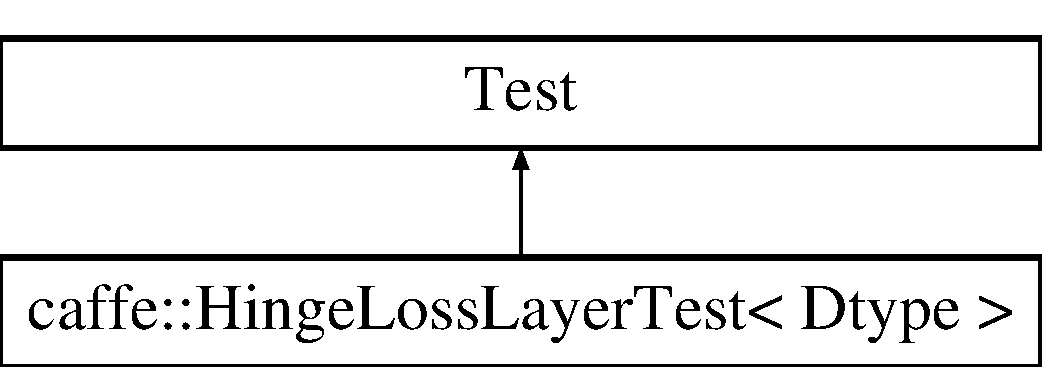
\includegraphics[height=2.000000cm]{classcaffe_1_1_hinge_loss_layer_test}
\end{center}
\end{figure}
\subsection*{Protected Member Functions}
\begin{DoxyCompactItemize}
\item 
\hyperlink{classcaffe_1_1_hinge_loss_layer_test_a0f145b65fe5c9f18761e27640c23ea1c}{Hinge\+Loss\+Layer\+Test} ()
\item 
virtual \hyperlink{classcaffe_1_1_hinge_loss_layer_test_af3418152e64659da16a3a5ed31c6721a}{$\sim$\+Hinge\+Loss\+Layer\+Test} ()
\end{DoxyCompactItemize}
\subsection*{Protected Attributes}
\begin{DoxyCompactItemize}
\item 
\hyperlink{classcaffe_1_1_blob}{Blob}$<$ Dtype $>$ $\ast$const \hyperlink{classcaffe_1_1_hinge_loss_layer_test_a86c856e37099156adab0197c38ce74ec}{blob\+\_\+bottom\+\_\+data\+\_\+}
\item 
\hyperlink{classcaffe_1_1_blob}{Blob}$<$ Dtype $>$ $\ast$const \hyperlink{classcaffe_1_1_hinge_loss_layer_test_a67cfd73cc1d49d8c959d05da2a5e15ef}{blob\+\_\+bottom\+\_\+label\+\_\+}
\item 
vector$<$ \hyperlink{classcaffe_1_1_blob}{Blob}$<$ Dtype $>$ $\ast$ $>$ \hyperlink{classcaffe_1_1_hinge_loss_layer_test_a9ab9805216e3120f98b6fd151c715ece}{blob\+\_\+bottom\+\_\+vec\+\_\+}
\item 
vector$<$ \hyperlink{classcaffe_1_1_blob}{Blob}$<$ Dtype $>$ $\ast$ $>$ \hyperlink{classcaffe_1_1_hinge_loss_layer_test_ae5653c7c55dff58664cfe3ad8093757e}{blob\+\_\+top\+\_\+vec\+\_\+}
\end{DoxyCompactItemize}


\subsection{Constructor \& Destructor Documentation}
\hypertarget{classcaffe_1_1_hinge_loss_layer_test_a0f145b65fe5c9f18761e27640c23ea1c}{\index{caffe\+::\+Hinge\+Loss\+Layer\+Test@{caffe\+::\+Hinge\+Loss\+Layer\+Test}!Hinge\+Loss\+Layer\+Test@{Hinge\+Loss\+Layer\+Test}}
\index{Hinge\+Loss\+Layer\+Test@{Hinge\+Loss\+Layer\+Test}!caffe\+::\+Hinge\+Loss\+Layer\+Test@{caffe\+::\+Hinge\+Loss\+Layer\+Test}}
\subsubsection[{Hinge\+Loss\+Layer\+Test}]{\setlength{\rightskip}{0pt plus 5cm}template$<$typename Dtype $>$ {\bf caffe\+::\+Hinge\+Loss\+Layer\+Test}$<$ Dtype $>$\+::{\bf Hinge\+Loss\+Layer\+Test} (
\begin{DoxyParamCaption}
{}
\end{DoxyParamCaption}
)\hspace{0.3cm}{\ttfamily [inline]}, {\ttfamily [protected]}}}\label{classcaffe_1_1_hinge_loss_layer_test_a0f145b65fe5c9f18761e27640c23ea1c}
\hypertarget{classcaffe_1_1_hinge_loss_layer_test_af3418152e64659da16a3a5ed31c6721a}{\index{caffe\+::\+Hinge\+Loss\+Layer\+Test@{caffe\+::\+Hinge\+Loss\+Layer\+Test}!````~Hinge\+Loss\+Layer\+Test@{$\sim$\+Hinge\+Loss\+Layer\+Test}}
\index{````~Hinge\+Loss\+Layer\+Test@{$\sim$\+Hinge\+Loss\+Layer\+Test}!caffe\+::\+Hinge\+Loss\+Layer\+Test@{caffe\+::\+Hinge\+Loss\+Layer\+Test}}
\subsubsection[{$\sim$\+Hinge\+Loss\+Layer\+Test}]{\setlength{\rightskip}{0pt plus 5cm}template$<$typename Dtype $>$ virtual {\bf caffe\+::\+Hinge\+Loss\+Layer\+Test}$<$ Dtype $>$\+::$\sim${\bf Hinge\+Loss\+Layer\+Test} (
\begin{DoxyParamCaption}
{}
\end{DoxyParamCaption}
)\hspace{0.3cm}{\ttfamily [inline]}, {\ttfamily [protected]}, {\ttfamily [virtual]}}}\label{classcaffe_1_1_hinge_loss_layer_test_af3418152e64659da16a3a5ed31c6721a}


\subsection{Member Data Documentation}
\hypertarget{classcaffe_1_1_hinge_loss_layer_test_a86c856e37099156adab0197c38ce74ec}{\index{caffe\+::\+Hinge\+Loss\+Layer\+Test@{caffe\+::\+Hinge\+Loss\+Layer\+Test}!blob\+\_\+bottom\+\_\+data\+\_\+@{blob\+\_\+bottom\+\_\+data\+\_\+}}
\index{blob\+\_\+bottom\+\_\+data\+\_\+@{blob\+\_\+bottom\+\_\+data\+\_\+}!caffe\+::\+Hinge\+Loss\+Layer\+Test@{caffe\+::\+Hinge\+Loss\+Layer\+Test}}
\subsubsection[{blob\+\_\+bottom\+\_\+data\+\_\+}]{\setlength{\rightskip}{0pt plus 5cm}template$<$typename Dtype $>$ {\bf Blob}$<$Dtype$>$$\ast$ const {\bf caffe\+::\+Hinge\+Loss\+Layer\+Test}$<$ Dtype $>$\+::blob\+\_\+bottom\+\_\+data\+\_\+\hspace{0.3cm}{\ttfamily [protected]}}}\label{classcaffe_1_1_hinge_loss_layer_test_a86c856e37099156adab0197c38ce74ec}
\hypertarget{classcaffe_1_1_hinge_loss_layer_test_a67cfd73cc1d49d8c959d05da2a5e15ef}{\index{caffe\+::\+Hinge\+Loss\+Layer\+Test@{caffe\+::\+Hinge\+Loss\+Layer\+Test}!blob\+\_\+bottom\+\_\+label\+\_\+@{blob\+\_\+bottom\+\_\+label\+\_\+}}
\index{blob\+\_\+bottom\+\_\+label\+\_\+@{blob\+\_\+bottom\+\_\+label\+\_\+}!caffe\+::\+Hinge\+Loss\+Layer\+Test@{caffe\+::\+Hinge\+Loss\+Layer\+Test}}
\subsubsection[{blob\+\_\+bottom\+\_\+label\+\_\+}]{\setlength{\rightskip}{0pt plus 5cm}template$<$typename Dtype $>$ {\bf Blob}$<$Dtype$>$$\ast$ const {\bf caffe\+::\+Hinge\+Loss\+Layer\+Test}$<$ Dtype $>$\+::blob\+\_\+bottom\+\_\+label\+\_\+\hspace{0.3cm}{\ttfamily [protected]}}}\label{classcaffe_1_1_hinge_loss_layer_test_a67cfd73cc1d49d8c959d05da2a5e15ef}
\hypertarget{classcaffe_1_1_hinge_loss_layer_test_a9ab9805216e3120f98b6fd151c715ece}{\index{caffe\+::\+Hinge\+Loss\+Layer\+Test@{caffe\+::\+Hinge\+Loss\+Layer\+Test}!blob\+\_\+bottom\+\_\+vec\+\_\+@{blob\+\_\+bottom\+\_\+vec\+\_\+}}
\index{blob\+\_\+bottom\+\_\+vec\+\_\+@{blob\+\_\+bottom\+\_\+vec\+\_\+}!caffe\+::\+Hinge\+Loss\+Layer\+Test@{caffe\+::\+Hinge\+Loss\+Layer\+Test}}
\subsubsection[{blob\+\_\+bottom\+\_\+vec\+\_\+}]{\setlength{\rightskip}{0pt plus 5cm}template$<$typename Dtype $>$ vector$<${\bf Blob}$<$Dtype$>$$\ast$$>$ {\bf caffe\+::\+Hinge\+Loss\+Layer\+Test}$<$ Dtype $>$\+::blob\+\_\+bottom\+\_\+vec\+\_\+\hspace{0.3cm}{\ttfamily [protected]}}}\label{classcaffe_1_1_hinge_loss_layer_test_a9ab9805216e3120f98b6fd151c715ece}
\hypertarget{classcaffe_1_1_hinge_loss_layer_test_ae5653c7c55dff58664cfe3ad8093757e}{\index{caffe\+::\+Hinge\+Loss\+Layer\+Test@{caffe\+::\+Hinge\+Loss\+Layer\+Test}!blob\+\_\+top\+\_\+vec\+\_\+@{blob\+\_\+top\+\_\+vec\+\_\+}}
\index{blob\+\_\+top\+\_\+vec\+\_\+@{blob\+\_\+top\+\_\+vec\+\_\+}!caffe\+::\+Hinge\+Loss\+Layer\+Test@{caffe\+::\+Hinge\+Loss\+Layer\+Test}}
\subsubsection[{blob\+\_\+top\+\_\+vec\+\_\+}]{\setlength{\rightskip}{0pt plus 5cm}template$<$typename Dtype $>$ vector$<${\bf Blob}$<$Dtype$>$$\ast$$>$ {\bf caffe\+::\+Hinge\+Loss\+Layer\+Test}$<$ Dtype $>$\+::blob\+\_\+top\+\_\+vec\+\_\+\hspace{0.3cm}{\ttfamily [protected]}}}\label{classcaffe_1_1_hinge_loss_layer_test_ae5653c7c55dff58664cfe3ad8093757e}


The documentation for this class was generated from the following file\+:\begin{DoxyCompactItemize}
\item 
src/caffe/test/\hyperlink{test__hinge__loss__layer_8cpp}{test\+\_\+hinge\+\_\+loss\+\_\+layer.\+cpp}\end{DoxyCompactItemize}

\hypertarget{classcaffe_1_1_im2col_layer}{\section{caffe\+:\+:Im2col\+Layer$<$ Dtype $>$ Class Template Reference}
\label{classcaffe_1_1_im2col_layer}\index{caffe\+::\+Im2col\+Layer$<$ Dtype $>$@{caffe\+::\+Im2col\+Layer$<$ Dtype $>$}}
}


{\ttfamily \#include $<$vision\+\_\+layers.\+hpp$>$}

Inheritance diagram for caffe\+:\+:Im2col\+Layer$<$ Dtype $>$\+:\begin{figure}[H]
\begin{center}
\leavevmode
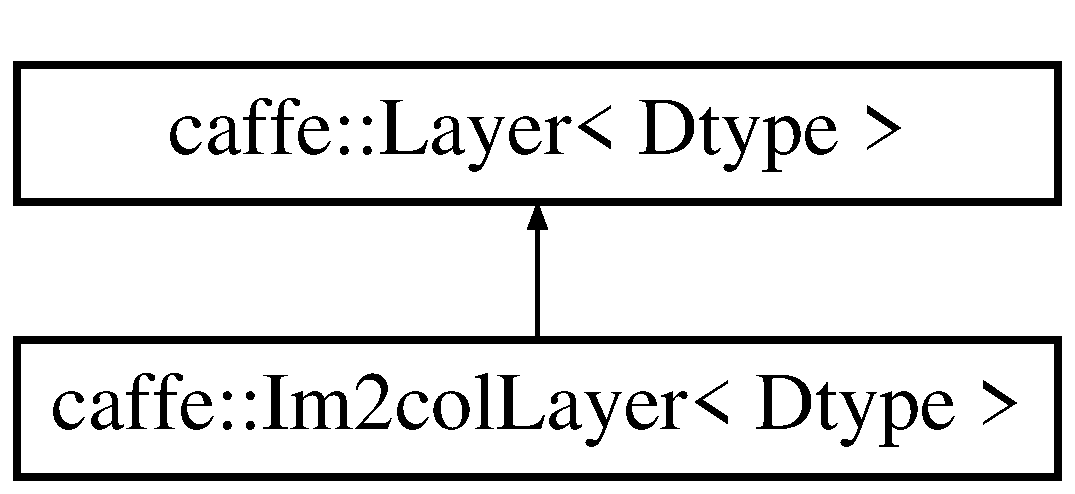
\includegraphics[height=2.000000cm]{classcaffe_1_1_im2col_layer}
\end{center}
\end{figure}
\subsection*{Public Member Functions}
\begin{DoxyCompactItemize}
\item 
\hyperlink{classcaffe_1_1_im2col_layer_aec089ca3ca3caf3d32193b9dcb2f98e1}{Im2col\+Layer} (const Layer\+Parameter \&param)
\item 
virtual void \hyperlink{classcaffe_1_1_im2col_layer_a869008ef04af4d7aed3e412e449b1aeb}{Set\+Up} (const vector$<$ \hyperlink{classcaffe_1_1_blob}{Blob}$<$ Dtype $>$ $\ast$ $>$ \&bottom, vector$<$ \hyperlink{classcaffe_1_1_blob}{Blob}$<$ Dtype $>$ $\ast$ $>$ $\ast$top)
\end{DoxyCompactItemize}
\subsection*{Protected Member Functions}
\begin{DoxyCompactItemize}
\item 
virtual Dtype \hyperlink{classcaffe_1_1_im2col_layer_a635af15bcfdf2ec96913d75de5763328}{Forward\+\_\+cpu} (const vector$<$ \hyperlink{classcaffe_1_1_blob}{Blob}$<$ Dtype $>$ $\ast$ $>$ \&bottom, vector$<$ \hyperlink{classcaffe_1_1_blob}{Blob}$<$ Dtype $>$ $\ast$ $>$ $\ast$top)
\item 
virtual Dtype \hyperlink{classcaffe_1_1_im2col_layer_af60c215a0953742dc1ca2163f55bd9a7}{Forward\+\_\+gpu} (const vector$<$ \hyperlink{classcaffe_1_1_blob}{Blob}$<$ Dtype $>$ $\ast$ $>$ \&bottom, vector$<$ \hyperlink{classcaffe_1_1_blob}{Blob}$<$ Dtype $>$ $\ast$ $>$ $\ast$top)
\item 
virtual void \hyperlink{classcaffe_1_1_im2col_layer_ae6436f4287c23e62965f7c8216669ef2}{Backward\+\_\+cpu} (const vector$<$ \hyperlink{classcaffe_1_1_blob}{Blob}$<$ Dtype $>$ $\ast$ $>$ \&top, const bool propagate\+\_\+down, vector$<$ \hyperlink{classcaffe_1_1_blob}{Blob}$<$ Dtype $>$ $\ast$ $>$ $\ast$bottom)
\item 
virtual void \hyperlink{classcaffe_1_1_im2col_layer_abe4feb385c1226f2d69ec47142ce0b06}{Backward\+\_\+gpu} (const vector$<$ \hyperlink{classcaffe_1_1_blob}{Blob}$<$ Dtype $>$ $\ast$ $>$ \&top, const bool propagate\+\_\+down, vector$<$ \hyperlink{classcaffe_1_1_blob}{Blob}$<$ Dtype $>$ $\ast$ $>$ $\ast$bottom)
\end{DoxyCompactItemize}
\subsection*{Protected Attributes}
\begin{DoxyCompactItemize}
\item 
int \hyperlink{classcaffe_1_1_im2col_layer_af4cb2dc9a9691d840dc5b18ddca5f3f3}{kernel\+\_\+size\+\_\+}
\item 
int \hyperlink{classcaffe_1_1_im2col_layer_a03923aa2de104271d4df535316871b3b}{stride\+\_\+}
\item 
int \hyperlink{classcaffe_1_1_im2col_layer_a819581a35ffba22f5df2c0340210c2e9}{channels\+\_\+}
\item 
int \hyperlink{classcaffe_1_1_im2col_layer_ade34e2397b55eb5687a32c9e59137ca9}{height\+\_\+}
\item 
int \hyperlink{classcaffe_1_1_im2col_layer_a6d888c45c786826e1acabd97213e45a6}{width\+\_\+}
\item 
int \hyperlink{classcaffe_1_1_im2col_layer_a37ed956e35a1b04a3c0da7363aa9ea1f}{pad\+\_\+}
\end{DoxyCompactItemize}


\subsection{Constructor \& Destructor Documentation}
\hypertarget{classcaffe_1_1_im2col_layer_aec089ca3ca3caf3d32193b9dcb2f98e1}{\index{caffe\+::\+Im2col\+Layer@{caffe\+::\+Im2col\+Layer}!Im2col\+Layer@{Im2col\+Layer}}
\index{Im2col\+Layer@{Im2col\+Layer}!caffe\+::\+Im2col\+Layer@{caffe\+::\+Im2col\+Layer}}
\subsubsection[{Im2col\+Layer}]{\setlength{\rightskip}{0pt plus 5cm}template$<$typename Dtype $>$ {\bf caffe\+::\+Im2col\+Layer}$<$ Dtype $>$\+::{\bf Im2col\+Layer} (
\begin{DoxyParamCaption}
\item[{const Layer\+Parameter \&}]{param}
\end{DoxyParamCaption}
)\hspace{0.3cm}{\ttfamily [inline]}, {\ttfamily [explicit]}}}\label{classcaffe_1_1_im2col_layer_aec089ca3ca3caf3d32193b9dcb2f98e1}


\subsection{Member Function Documentation}
\hypertarget{classcaffe_1_1_im2col_layer_ae6436f4287c23e62965f7c8216669ef2}{\index{caffe\+::\+Im2col\+Layer@{caffe\+::\+Im2col\+Layer}!Backward\+\_\+cpu@{Backward\+\_\+cpu}}
\index{Backward\+\_\+cpu@{Backward\+\_\+cpu}!caffe\+::\+Im2col\+Layer@{caffe\+::\+Im2col\+Layer}}
\subsubsection[{Backward\+\_\+cpu}]{\setlength{\rightskip}{0pt plus 5cm}template$<$typename Dtype $>$ void {\bf caffe\+::\+Im2col\+Layer}$<$ Dtype $>$\+::Backward\+\_\+cpu (
\begin{DoxyParamCaption}
\item[{const vector$<$ {\bf Blob}$<$ Dtype $>$ $\ast$ $>$ \&}]{top, }
\item[{const bool}]{propagate\+\_\+down, }
\item[{vector$<$ {\bf Blob}$<$ Dtype $>$ $\ast$ $>$ $\ast$}]{bottom}
\end{DoxyParamCaption}
)\hspace{0.3cm}{\ttfamily [protected]}, {\ttfamily [virtual]}}}\label{classcaffe_1_1_im2col_layer_ae6436f4287c23e62965f7c8216669ef2}


Implements \hyperlink{classcaffe_1_1_layer_ac2d82011d076237c67997f63e7ee4b80}{caffe\+::\+Layer$<$ Dtype $>$}.

\hypertarget{classcaffe_1_1_im2col_layer_abe4feb385c1226f2d69ec47142ce0b06}{\index{caffe\+::\+Im2col\+Layer@{caffe\+::\+Im2col\+Layer}!Backward\+\_\+gpu@{Backward\+\_\+gpu}}
\index{Backward\+\_\+gpu@{Backward\+\_\+gpu}!caffe\+::\+Im2col\+Layer@{caffe\+::\+Im2col\+Layer}}
\subsubsection[{Backward\+\_\+gpu}]{\setlength{\rightskip}{0pt plus 5cm}template$<$typename Dtype $>$ void {\bf caffe\+::\+Im2col\+Layer}$<$ Dtype $>$\+::Backward\+\_\+gpu (
\begin{DoxyParamCaption}
\item[{const vector$<$ {\bf Blob}$<$ Dtype $>$ $\ast$ $>$ \&}]{top, }
\item[{const bool}]{propagate\+\_\+down, }
\item[{vector$<$ {\bf Blob}$<$ Dtype $>$ $\ast$ $>$ $\ast$}]{bottom}
\end{DoxyParamCaption}
)\hspace{0.3cm}{\ttfamily [protected]}, {\ttfamily [virtual]}}}\label{classcaffe_1_1_im2col_layer_abe4feb385c1226f2d69ec47142ce0b06}


Reimplemented from \hyperlink{classcaffe_1_1_layer_adf07ffe1f22d2fd2b1b0ff475ef5a64b}{caffe\+::\+Layer$<$ Dtype $>$}.

\hypertarget{classcaffe_1_1_im2col_layer_a635af15bcfdf2ec96913d75de5763328}{\index{caffe\+::\+Im2col\+Layer@{caffe\+::\+Im2col\+Layer}!Forward\+\_\+cpu@{Forward\+\_\+cpu}}
\index{Forward\+\_\+cpu@{Forward\+\_\+cpu}!caffe\+::\+Im2col\+Layer@{caffe\+::\+Im2col\+Layer}}
\subsubsection[{Forward\+\_\+cpu}]{\setlength{\rightskip}{0pt plus 5cm}template$<$typename Dtype $>$ Dtype {\bf caffe\+::\+Im2col\+Layer}$<$ Dtype $>$\+::Forward\+\_\+cpu (
\begin{DoxyParamCaption}
\item[{const vector$<$ {\bf Blob}$<$ Dtype $>$ $\ast$ $>$ \&}]{bottom, }
\item[{vector$<$ {\bf Blob}$<$ Dtype $>$ $\ast$ $>$ $\ast$}]{top}
\end{DoxyParamCaption}
)\hspace{0.3cm}{\ttfamily [protected]}, {\ttfamily [virtual]}}}\label{classcaffe_1_1_im2col_layer_a635af15bcfdf2ec96913d75de5763328}


Implements \hyperlink{classcaffe_1_1_layer_a8f7f61da3b8b3ca7f2394dee33873353}{caffe\+::\+Layer$<$ Dtype $>$}.

\hypertarget{classcaffe_1_1_im2col_layer_af60c215a0953742dc1ca2163f55bd9a7}{\index{caffe\+::\+Im2col\+Layer@{caffe\+::\+Im2col\+Layer}!Forward\+\_\+gpu@{Forward\+\_\+gpu}}
\index{Forward\+\_\+gpu@{Forward\+\_\+gpu}!caffe\+::\+Im2col\+Layer@{caffe\+::\+Im2col\+Layer}}
\subsubsection[{Forward\+\_\+gpu}]{\setlength{\rightskip}{0pt plus 5cm}template$<$typename Dtype $>$ Dtype {\bf caffe\+::\+Im2col\+Layer}$<$ Dtype $>$\+::Forward\+\_\+gpu (
\begin{DoxyParamCaption}
\item[{const vector$<$ {\bf Blob}$<$ Dtype $>$ $\ast$ $>$ \&}]{bottom, }
\item[{vector$<$ {\bf Blob}$<$ Dtype $>$ $\ast$ $>$ $\ast$}]{top}
\end{DoxyParamCaption}
)\hspace{0.3cm}{\ttfamily [protected]}, {\ttfamily [virtual]}}}\label{classcaffe_1_1_im2col_layer_af60c215a0953742dc1ca2163f55bd9a7}


Reimplemented from \hyperlink{classcaffe_1_1_layer_a2d78dbf5d8bc36928bd8f6fcfbafbcef}{caffe\+::\+Layer$<$ Dtype $>$}.

\hypertarget{classcaffe_1_1_im2col_layer_a869008ef04af4d7aed3e412e449b1aeb}{\index{caffe\+::\+Im2col\+Layer@{caffe\+::\+Im2col\+Layer}!Set\+Up@{Set\+Up}}
\index{Set\+Up@{Set\+Up}!caffe\+::\+Im2col\+Layer@{caffe\+::\+Im2col\+Layer}}
\subsubsection[{Set\+Up}]{\setlength{\rightskip}{0pt plus 5cm}template$<$typename Dtype $>$ void {\bf caffe\+::\+Im2col\+Layer}$<$ Dtype $>$\+::Set\+Up (
\begin{DoxyParamCaption}
\item[{const vector$<$ {\bf Blob}$<$ Dtype $>$ $\ast$ $>$ \&}]{bottom, }
\item[{vector$<$ {\bf Blob}$<$ Dtype $>$ $\ast$ $>$ $\ast$}]{top}
\end{DoxyParamCaption}
)\hspace{0.3cm}{\ttfamily [virtual]}}}\label{classcaffe_1_1_im2col_layer_a869008ef04af4d7aed3e412e449b1aeb}


Implements \hyperlink{classcaffe_1_1_layer_abd13c6489c13953b4fbcfcf6880835d0}{caffe\+::\+Layer$<$ Dtype $>$}.



\subsection{Member Data Documentation}
\hypertarget{classcaffe_1_1_im2col_layer_a819581a35ffba22f5df2c0340210c2e9}{\index{caffe\+::\+Im2col\+Layer@{caffe\+::\+Im2col\+Layer}!channels\+\_\+@{channels\+\_\+}}
\index{channels\+\_\+@{channels\+\_\+}!caffe\+::\+Im2col\+Layer@{caffe\+::\+Im2col\+Layer}}
\subsubsection[{channels\+\_\+}]{\setlength{\rightskip}{0pt plus 5cm}template$<$typename Dtype $>$ int {\bf caffe\+::\+Im2col\+Layer}$<$ Dtype $>$\+::channels\+\_\+\hspace{0.3cm}{\ttfamily [protected]}}}\label{classcaffe_1_1_im2col_layer_a819581a35ffba22f5df2c0340210c2e9}
\hypertarget{classcaffe_1_1_im2col_layer_ade34e2397b55eb5687a32c9e59137ca9}{\index{caffe\+::\+Im2col\+Layer@{caffe\+::\+Im2col\+Layer}!height\+\_\+@{height\+\_\+}}
\index{height\+\_\+@{height\+\_\+}!caffe\+::\+Im2col\+Layer@{caffe\+::\+Im2col\+Layer}}
\subsubsection[{height\+\_\+}]{\setlength{\rightskip}{0pt plus 5cm}template$<$typename Dtype $>$ int {\bf caffe\+::\+Im2col\+Layer}$<$ Dtype $>$\+::height\+\_\+\hspace{0.3cm}{\ttfamily [protected]}}}\label{classcaffe_1_1_im2col_layer_ade34e2397b55eb5687a32c9e59137ca9}
\hypertarget{classcaffe_1_1_im2col_layer_af4cb2dc9a9691d840dc5b18ddca5f3f3}{\index{caffe\+::\+Im2col\+Layer@{caffe\+::\+Im2col\+Layer}!kernel\+\_\+size\+\_\+@{kernel\+\_\+size\+\_\+}}
\index{kernel\+\_\+size\+\_\+@{kernel\+\_\+size\+\_\+}!caffe\+::\+Im2col\+Layer@{caffe\+::\+Im2col\+Layer}}
\subsubsection[{kernel\+\_\+size\+\_\+}]{\setlength{\rightskip}{0pt plus 5cm}template$<$typename Dtype $>$ int {\bf caffe\+::\+Im2col\+Layer}$<$ Dtype $>$\+::kernel\+\_\+size\+\_\+\hspace{0.3cm}{\ttfamily [protected]}}}\label{classcaffe_1_1_im2col_layer_af4cb2dc9a9691d840dc5b18ddca5f3f3}
\hypertarget{classcaffe_1_1_im2col_layer_a37ed956e35a1b04a3c0da7363aa9ea1f}{\index{caffe\+::\+Im2col\+Layer@{caffe\+::\+Im2col\+Layer}!pad\+\_\+@{pad\+\_\+}}
\index{pad\+\_\+@{pad\+\_\+}!caffe\+::\+Im2col\+Layer@{caffe\+::\+Im2col\+Layer}}
\subsubsection[{pad\+\_\+}]{\setlength{\rightskip}{0pt plus 5cm}template$<$typename Dtype $>$ int {\bf caffe\+::\+Im2col\+Layer}$<$ Dtype $>$\+::pad\+\_\+\hspace{0.3cm}{\ttfamily [protected]}}}\label{classcaffe_1_1_im2col_layer_a37ed956e35a1b04a3c0da7363aa9ea1f}
\hypertarget{classcaffe_1_1_im2col_layer_a03923aa2de104271d4df535316871b3b}{\index{caffe\+::\+Im2col\+Layer@{caffe\+::\+Im2col\+Layer}!stride\+\_\+@{stride\+\_\+}}
\index{stride\+\_\+@{stride\+\_\+}!caffe\+::\+Im2col\+Layer@{caffe\+::\+Im2col\+Layer}}
\subsubsection[{stride\+\_\+}]{\setlength{\rightskip}{0pt plus 5cm}template$<$typename Dtype $>$ int {\bf caffe\+::\+Im2col\+Layer}$<$ Dtype $>$\+::stride\+\_\+\hspace{0.3cm}{\ttfamily [protected]}}}\label{classcaffe_1_1_im2col_layer_a03923aa2de104271d4df535316871b3b}
\hypertarget{classcaffe_1_1_im2col_layer_a6d888c45c786826e1acabd97213e45a6}{\index{caffe\+::\+Im2col\+Layer@{caffe\+::\+Im2col\+Layer}!width\+\_\+@{width\+\_\+}}
\index{width\+\_\+@{width\+\_\+}!caffe\+::\+Im2col\+Layer@{caffe\+::\+Im2col\+Layer}}
\subsubsection[{width\+\_\+}]{\setlength{\rightskip}{0pt plus 5cm}template$<$typename Dtype $>$ int {\bf caffe\+::\+Im2col\+Layer}$<$ Dtype $>$\+::width\+\_\+\hspace{0.3cm}{\ttfamily [protected]}}}\label{classcaffe_1_1_im2col_layer_a6d888c45c786826e1acabd97213e45a6}


The documentation for this class was generated from the following files\+:\begin{DoxyCompactItemize}
\item 
include/caffe/\hyperlink{vision__layers_8hpp}{vision\+\_\+layers.\+hpp}\item 
src/caffe/layers/\hyperlink{im2col__layer_8cpp}{im2col\+\_\+layer.\+cpp}\item 
src/caffe/layers/\hyperlink{im2col__layer_8cu}{im2col\+\_\+layer.\+cu}\end{DoxyCompactItemize}

\hypertarget{classcaffe_1_1_im2col_layer_test}{\section{caffe\+:\+:Im2col\+Layer\+Test$<$ Dtype $>$ Class Template Reference}
\label{classcaffe_1_1_im2col_layer_test}\index{caffe\+::\+Im2col\+Layer\+Test$<$ Dtype $>$@{caffe\+::\+Im2col\+Layer\+Test$<$ Dtype $>$}}
}
Inheritance diagram for caffe\+:\+:Im2col\+Layer\+Test$<$ Dtype $>$\+:\begin{figure}[H]
\begin{center}
\leavevmode
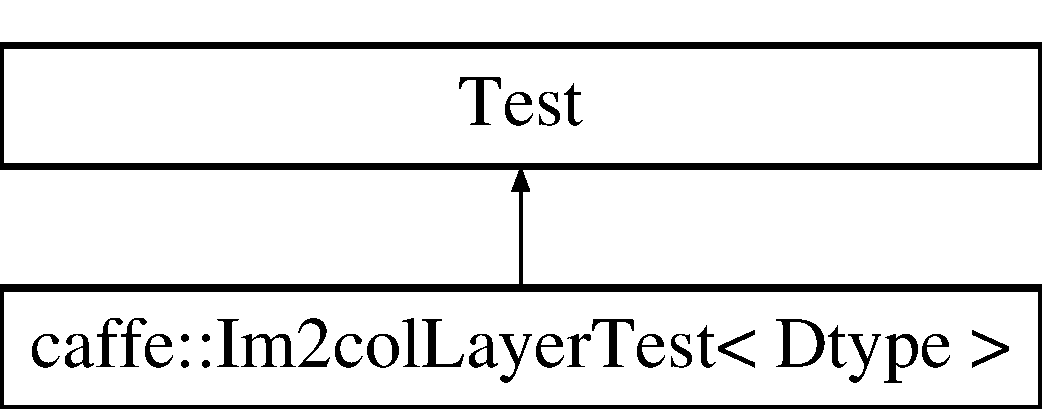
\includegraphics[height=2.000000cm]{classcaffe_1_1_im2col_layer_test}
\end{center}
\end{figure}
\subsection*{Protected Member Functions}
\begin{DoxyCompactItemize}
\item 
\hyperlink{classcaffe_1_1_im2col_layer_test_a2651ce41b8c4202a776aabf0045b9979}{Im2col\+Layer\+Test} ()
\item 
virtual \hyperlink{classcaffe_1_1_im2col_layer_test_a2e3fa23c7c2cc695780e8bdd48c50f74}{$\sim$\+Im2col\+Layer\+Test} ()
\end{DoxyCompactItemize}
\subsection*{Protected Attributes}
\begin{DoxyCompactItemize}
\item 
\hyperlink{classcaffe_1_1_blob}{Blob}$<$ Dtype $>$ $\ast$const \hyperlink{classcaffe_1_1_im2col_layer_test_a8dcff9e3ad57f57c4e1ca6771be34554}{blob\+\_\+bottom\+\_\+}
\item 
\hyperlink{classcaffe_1_1_blob}{Blob}$<$ Dtype $>$ $\ast$const \hyperlink{classcaffe_1_1_im2col_layer_test_a04f605a94d9b6ead927c47c754b459b2}{blob\+\_\+top\+\_\+}
\item 
vector$<$ \hyperlink{classcaffe_1_1_blob}{Blob}$<$ Dtype $>$ $\ast$ $>$ \hyperlink{classcaffe_1_1_im2col_layer_test_ac9dfa820b4759b538a459cb5429943b1}{blob\+\_\+bottom\+\_\+vec\+\_\+}
\item 
vector$<$ \hyperlink{classcaffe_1_1_blob}{Blob}$<$ Dtype $>$ $\ast$ $>$ \hyperlink{classcaffe_1_1_im2col_layer_test_ac2f2ec2988cd9149e50dd366957d830e}{blob\+\_\+top\+\_\+vec\+\_\+}
\end{DoxyCompactItemize}


\subsection{Constructor \& Destructor Documentation}
\hypertarget{classcaffe_1_1_im2col_layer_test_a2651ce41b8c4202a776aabf0045b9979}{\index{caffe\+::\+Im2col\+Layer\+Test@{caffe\+::\+Im2col\+Layer\+Test}!Im2col\+Layer\+Test@{Im2col\+Layer\+Test}}
\index{Im2col\+Layer\+Test@{Im2col\+Layer\+Test}!caffe\+::\+Im2col\+Layer\+Test@{caffe\+::\+Im2col\+Layer\+Test}}
\subsubsection[{Im2col\+Layer\+Test}]{\setlength{\rightskip}{0pt plus 5cm}template$<$typename Dtype $>$ {\bf caffe\+::\+Im2col\+Layer\+Test}$<$ Dtype $>$\+::{\bf Im2col\+Layer\+Test} (
\begin{DoxyParamCaption}
{}
\end{DoxyParamCaption}
)\hspace{0.3cm}{\ttfamily [inline]}, {\ttfamily [protected]}}}\label{classcaffe_1_1_im2col_layer_test_a2651ce41b8c4202a776aabf0045b9979}
\hypertarget{classcaffe_1_1_im2col_layer_test_a2e3fa23c7c2cc695780e8bdd48c50f74}{\index{caffe\+::\+Im2col\+Layer\+Test@{caffe\+::\+Im2col\+Layer\+Test}!````~Im2col\+Layer\+Test@{$\sim$\+Im2col\+Layer\+Test}}
\index{````~Im2col\+Layer\+Test@{$\sim$\+Im2col\+Layer\+Test}!caffe\+::\+Im2col\+Layer\+Test@{caffe\+::\+Im2col\+Layer\+Test}}
\subsubsection[{$\sim$\+Im2col\+Layer\+Test}]{\setlength{\rightskip}{0pt plus 5cm}template$<$typename Dtype $>$ virtual {\bf caffe\+::\+Im2col\+Layer\+Test}$<$ Dtype $>$\+::$\sim${\bf Im2col\+Layer\+Test} (
\begin{DoxyParamCaption}
{}
\end{DoxyParamCaption}
)\hspace{0.3cm}{\ttfamily [inline]}, {\ttfamily [protected]}, {\ttfamily [virtual]}}}\label{classcaffe_1_1_im2col_layer_test_a2e3fa23c7c2cc695780e8bdd48c50f74}


\subsection{Member Data Documentation}
\hypertarget{classcaffe_1_1_im2col_layer_test_a8dcff9e3ad57f57c4e1ca6771be34554}{\index{caffe\+::\+Im2col\+Layer\+Test@{caffe\+::\+Im2col\+Layer\+Test}!blob\+\_\+bottom\+\_\+@{blob\+\_\+bottom\+\_\+}}
\index{blob\+\_\+bottom\+\_\+@{blob\+\_\+bottom\+\_\+}!caffe\+::\+Im2col\+Layer\+Test@{caffe\+::\+Im2col\+Layer\+Test}}
\subsubsection[{blob\+\_\+bottom\+\_\+}]{\setlength{\rightskip}{0pt plus 5cm}template$<$typename Dtype $>$ {\bf Blob}$<$Dtype$>$$\ast$ const {\bf caffe\+::\+Im2col\+Layer\+Test}$<$ Dtype $>$\+::blob\+\_\+bottom\+\_\+\hspace{0.3cm}{\ttfamily [protected]}}}\label{classcaffe_1_1_im2col_layer_test_a8dcff9e3ad57f57c4e1ca6771be34554}
\hypertarget{classcaffe_1_1_im2col_layer_test_ac9dfa820b4759b538a459cb5429943b1}{\index{caffe\+::\+Im2col\+Layer\+Test@{caffe\+::\+Im2col\+Layer\+Test}!blob\+\_\+bottom\+\_\+vec\+\_\+@{blob\+\_\+bottom\+\_\+vec\+\_\+}}
\index{blob\+\_\+bottom\+\_\+vec\+\_\+@{blob\+\_\+bottom\+\_\+vec\+\_\+}!caffe\+::\+Im2col\+Layer\+Test@{caffe\+::\+Im2col\+Layer\+Test}}
\subsubsection[{blob\+\_\+bottom\+\_\+vec\+\_\+}]{\setlength{\rightskip}{0pt plus 5cm}template$<$typename Dtype $>$ vector$<${\bf Blob}$<$Dtype$>$$\ast$$>$ {\bf caffe\+::\+Im2col\+Layer\+Test}$<$ Dtype $>$\+::blob\+\_\+bottom\+\_\+vec\+\_\+\hspace{0.3cm}{\ttfamily [protected]}}}\label{classcaffe_1_1_im2col_layer_test_ac9dfa820b4759b538a459cb5429943b1}
\hypertarget{classcaffe_1_1_im2col_layer_test_a04f605a94d9b6ead927c47c754b459b2}{\index{caffe\+::\+Im2col\+Layer\+Test@{caffe\+::\+Im2col\+Layer\+Test}!blob\+\_\+top\+\_\+@{blob\+\_\+top\+\_\+}}
\index{blob\+\_\+top\+\_\+@{blob\+\_\+top\+\_\+}!caffe\+::\+Im2col\+Layer\+Test@{caffe\+::\+Im2col\+Layer\+Test}}
\subsubsection[{blob\+\_\+top\+\_\+}]{\setlength{\rightskip}{0pt plus 5cm}template$<$typename Dtype $>$ {\bf Blob}$<$Dtype$>$$\ast$ const {\bf caffe\+::\+Im2col\+Layer\+Test}$<$ Dtype $>$\+::blob\+\_\+top\+\_\+\hspace{0.3cm}{\ttfamily [protected]}}}\label{classcaffe_1_1_im2col_layer_test_a04f605a94d9b6ead927c47c754b459b2}
\hypertarget{classcaffe_1_1_im2col_layer_test_ac2f2ec2988cd9149e50dd366957d830e}{\index{caffe\+::\+Im2col\+Layer\+Test@{caffe\+::\+Im2col\+Layer\+Test}!blob\+\_\+top\+\_\+vec\+\_\+@{blob\+\_\+top\+\_\+vec\+\_\+}}
\index{blob\+\_\+top\+\_\+vec\+\_\+@{blob\+\_\+top\+\_\+vec\+\_\+}!caffe\+::\+Im2col\+Layer\+Test@{caffe\+::\+Im2col\+Layer\+Test}}
\subsubsection[{blob\+\_\+top\+\_\+vec\+\_\+}]{\setlength{\rightskip}{0pt plus 5cm}template$<$typename Dtype $>$ vector$<${\bf Blob}$<$Dtype$>$$\ast$$>$ {\bf caffe\+::\+Im2col\+Layer\+Test}$<$ Dtype $>$\+::blob\+\_\+top\+\_\+vec\+\_\+\hspace{0.3cm}{\ttfamily [protected]}}}\label{classcaffe_1_1_im2col_layer_test_ac2f2ec2988cd9149e50dd366957d830e}


The documentation for this class was generated from the following file\+:\begin{DoxyCompactItemize}
\item 
src/caffe/test/\hyperlink{test__im2col__layer_8cpp}{test\+\_\+im2col\+\_\+layer.\+cpp}\end{DoxyCompactItemize}

\hypertarget{classcaffe_1_1_image_data_layer}{\section{caffe\+:\+:Image\+Data\+Layer$<$ Dtype $>$ Class Template Reference}
\label{classcaffe_1_1_image_data_layer}\index{caffe\+::\+Image\+Data\+Layer$<$ Dtype $>$@{caffe\+::\+Image\+Data\+Layer$<$ Dtype $>$}}
}


{\ttfamily \#include $<$vision\+\_\+layers.\+hpp$>$}

Inheritance diagram for caffe\+:\+:Image\+Data\+Layer$<$ Dtype $>$\+:\begin{figure}[H]
\begin{center}
\leavevmode
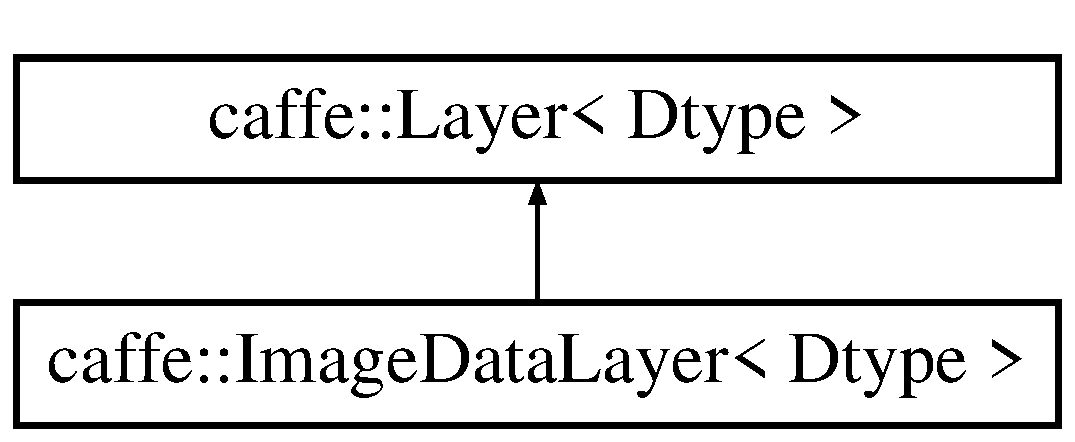
\includegraphics[height=2.000000cm]{classcaffe_1_1_image_data_layer}
\end{center}
\end{figure}
\subsection*{Public Member Functions}
\begin{DoxyCompactItemize}
\item 
\hyperlink{classcaffe_1_1_image_data_layer_a2319914181470f8ecd80ffb63d0daec9}{Image\+Data\+Layer} (const Layer\+Parameter \&param)
\item 
virtual \hyperlink{classcaffe_1_1_image_data_layer_a153c68c5d7da4ffcc1d563c89e0b7336}{$\sim$\+Image\+Data\+Layer} ()
\item 
virtual void \hyperlink{classcaffe_1_1_image_data_layer_a02eedd60b16ef4f2285cd75110a27226}{Set\+Up} (const vector$<$ \hyperlink{classcaffe_1_1_blob}{Blob}$<$ Dtype $>$ $\ast$ $>$ \&bottom, vector$<$ \hyperlink{classcaffe_1_1_blob}{Blob}$<$ Dtype $>$ $\ast$ $>$ $\ast$top)
\end{DoxyCompactItemize}
\subsection*{Protected Member Functions}
\begin{DoxyCompactItemize}
\item 
virtual Dtype \hyperlink{classcaffe_1_1_image_data_layer_a3093be55fa03cc281778ba230a05456c}{Forward\+\_\+cpu} (const vector$<$ \hyperlink{classcaffe_1_1_blob}{Blob}$<$ Dtype $>$ $\ast$ $>$ \&bottom, vector$<$ \hyperlink{classcaffe_1_1_blob}{Blob}$<$ Dtype $>$ $\ast$ $>$ $\ast$top)
\item 
virtual Dtype \hyperlink{classcaffe_1_1_image_data_layer_a3719ea4c463b83e57ae7249e5e371332}{Forward\+\_\+gpu} (const vector$<$ \hyperlink{classcaffe_1_1_blob}{Blob}$<$ Dtype $>$ $\ast$ $>$ \&bottom, vector$<$ \hyperlink{classcaffe_1_1_blob}{Blob}$<$ Dtype $>$ $\ast$ $>$ $\ast$top)
\item 
virtual void \hyperlink{classcaffe_1_1_image_data_layer_aa94c13be8dcceb317b637c6ddf6cb0af}{Backward\+\_\+cpu} (const vector$<$ \hyperlink{classcaffe_1_1_blob}{Blob}$<$ Dtype $>$ $\ast$ $>$ \&top, const bool propagate\+\_\+down, vector$<$ \hyperlink{classcaffe_1_1_blob}{Blob}$<$ Dtype $>$ $\ast$ $>$ $\ast$bottom)
\item 
virtual void \hyperlink{classcaffe_1_1_image_data_layer_af467793e1c2184cd5016186c54167a20}{Backward\+\_\+gpu} (const vector$<$ \hyperlink{classcaffe_1_1_blob}{Blob}$<$ Dtype $>$ $\ast$ $>$ \&top, const bool propagate\+\_\+down, vector$<$ \hyperlink{classcaffe_1_1_blob}{Blob}$<$ Dtype $>$ $\ast$ $>$ $\ast$bottom)
\item 
virtual void \hyperlink{classcaffe_1_1_image_data_layer_a4cb51cd6f7ea31801d59164683ec5f64}{Shuffle\+Images} ()
\item 
virtual void \hyperlink{classcaffe_1_1_image_data_layer_a969b897fd9790b11862353f1940e07c0}{Create\+Prefetch\+Thread} ()
\item 
virtual void \hyperlink{classcaffe_1_1_image_data_layer_aaee5437acbba47d4f48f87df96ce12c9}{Join\+Prefetch\+Thread} ()
\item 
virtual unsigned int \hyperlink{classcaffe_1_1_image_data_layer_ab7009e152a69b4ba4fef5c88311a6adf}{Prefetch\+Rand} ()
\end{DoxyCompactItemize}
\subsection*{Protected Attributes}
\begin{DoxyCompactItemize}
\item 
shared\+\_\+ptr$<$ \hyperlink{classcaffe_1_1_caffe_1_1_r_n_g}{Caffe\+::\+R\+N\+G} $>$ \hyperlink{classcaffe_1_1_image_data_layer_a57a7df530e562fa080923aab6c331ab9}{prefetch\+\_\+rng\+\_\+}
\item 
vector$<$ std\+::pair$<$ std\+::string, \\*
int $>$ $>$ \hyperlink{classcaffe_1_1_image_data_layer_a72002dc4459f0d7d739779d734a7c684}{lines\+\_\+}
\item 
int \hyperlink{classcaffe_1_1_image_data_layer_a943f32fdd8d0d37883500b6d83d4243f}{lines\+\_\+id\+\_\+}
\item 
int \hyperlink{classcaffe_1_1_image_data_layer_a6534d716642ef3d9d95d19de3c28cafb}{datum\+\_\+channels\+\_\+}
\item 
int \hyperlink{classcaffe_1_1_image_data_layer_a5eb0e9d6e6263a2c66f07f1218aeb2dd}{datum\+\_\+height\+\_\+}
\item 
int \hyperlink{classcaffe_1_1_image_data_layer_a0daa71d91a0c49e841b39e1a27112220}{datum\+\_\+width\+\_\+}
\item 
int \hyperlink{classcaffe_1_1_image_data_layer_acbfb83156d383dc61808c419e4005ad9}{datum\+\_\+size\+\_\+}
\item 
pthread\+\_\+t \hyperlink{classcaffe_1_1_image_data_layer_a4381ef240bd59045142746a3142e7583}{thread\+\_\+}
\item 
shared\+\_\+ptr$<$ \hyperlink{classcaffe_1_1_blob}{Blob}$<$ Dtype $>$ $>$ \hyperlink{classcaffe_1_1_image_data_layer_a5fdda88b05ef9bdf536544e5eb6931db}{prefetch\+\_\+data\+\_\+}
\item 
shared\+\_\+ptr$<$ \hyperlink{classcaffe_1_1_blob}{Blob}$<$ Dtype $>$ $>$ \hyperlink{classcaffe_1_1_image_data_layer_ab762b1b1fb4cfb2e8029eed41cb0ec03}{prefetch\+\_\+label\+\_\+}
\item 
\hyperlink{classcaffe_1_1_blob}{Blob}$<$ Dtype $>$ \hyperlink{classcaffe_1_1_image_data_layer_aad14555c38b6c3b7c9c4c7153c3b2006}{data\+\_\+mean\+\_\+}
\item 
\hyperlink{classcaffe_1_1_caffe_ad2993dccc4a615c39259ed7f0d0e24e9}{Caffe\+::\+Phase} \hyperlink{classcaffe_1_1_image_data_layer_ad16bb1500ecf69e5891f53794f565681}{phase\+\_\+}
\end{DoxyCompactItemize}
\subsection*{Friends}
\begin{DoxyCompactItemize}
\item 
void $\ast$ \hyperlink{classcaffe_1_1_image_data_layer_ae4bae78139298c78a305dcd72fd0895d}{Image\+Data\+Layer\+Prefetch} (void $\ast$layer\+\_\+pointer)
\end{DoxyCompactItemize}


\subsection{Constructor \& Destructor Documentation}
\hypertarget{classcaffe_1_1_image_data_layer_a2319914181470f8ecd80ffb63d0daec9}{\index{caffe\+::\+Image\+Data\+Layer@{caffe\+::\+Image\+Data\+Layer}!Image\+Data\+Layer@{Image\+Data\+Layer}}
\index{Image\+Data\+Layer@{Image\+Data\+Layer}!caffe\+::\+Image\+Data\+Layer@{caffe\+::\+Image\+Data\+Layer}}
\subsubsection[{Image\+Data\+Layer}]{\setlength{\rightskip}{0pt plus 5cm}template$<$typename Dtype $>$ {\bf caffe\+::\+Image\+Data\+Layer}$<$ Dtype $>$\+::{\bf Image\+Data\+Layer} (
\begin{DoxyParamCaption}
\item[{const Layer\+Parameter \&}]{param}
\end{DoxyParamCaption}
)\hspace{0.3cm}{\ttfamily [inline]}, {\ttfamily [explicit]}}}\label{classcaffe_1_1_image_data_layer_a2319914181470f8ecd80ffb63d0daec9}
\hypertarget{classcaffe_1_1_image_data_layer_a153c68c5d7da4ffcc1d563c89e0b7336}{\index{caffe\+::\+Image\+Data\+Layer@{caffe\+::\+Image\+Data\+Layer}!````~Image\+Data\+Layer@{$\sim$\+Image\+Data\+Layer}}
\index{````~Image\+Data\+Layer@{$\sim$\+Image\+Data\+Layer}!caffe\+::\+Image\+Data\+Layer@{caffe\+::\+Image\+Data\+Layer}}
\subsubsection[{$\sim$\+Image\+Data\+Layer}]{\setlength{\rightskip}{0pt plus 5cm}template$<$typename Dtype $>$ {\bf caffe\+::\+Image\+Data\+Layer}$<$ Dtype $>$\+::$\sim${\bf Image\+Data\+Layer}$<$ Dtype $>$ (
\begin{DoxyParamCaption}
{}
\end{DoxyParamCaption}
)\hspace{0.3cm}{\ttfamily [virtual]}}}\label{classcaffe_1_1_image_data_layer_a153c68c5d7da4ffcc1d563c89e0b7336}


\subsection{Member Function Documentation}
\hypertarget{classcaffe_1_1_image_data_layer_aa94c13be8dcceb317b637c6ddf6cb0af}{\index{caffe\+::\+Image\+Data\+Layer@{caffe\+::\+Image\+Data\+Layer}!Backward\+\_\+cpu@{Backward\+\_\+cpu}}
\index{Backward\+\_\+cpu@{Backward\+\_\+cpu}!caffe\+::\+Image\+Data\+Layer@{caffe\+::\+Image\+Data\+Layer}}
\subsubsection[{Backward\+\_\+cpu}]{\setlength{\rightskip}{0pt plus 5cm}template$<$typename Dtype $>$ virtual void {\bf caffe\+::\+Image\+Data\+Layer}$<$ Dtype $>$\+::Backward\+\_\+cpu (
\begin{DoxyParamCaption}
\item[{const vector$<$ {\bf Blob}$<$ Dtype $>$ $\ast$ $>$ \&}]{top, }
\item[{const bool}]{propagate\+\_\+down, }
\item[{vector$<$ {\bf Blob}$<$ Dtype $>$ $\ast$ $>$ $\ast$}]{bottom}
\end{DoxyParamCaption}
)\hspace{0.3cm}{\ttfamily [inline]}, {\ttfamily [protected]}, {\ttfamily [virtual]}}}\label{classcaffe_1_1_image_data_layer_aa94c13be8dcceb317b637c6ddf6cb0af}


Implements \hyperlink{classcaffe_1_1_layer_ac2d82011d076237c67997f63e7ee4b80}{caffe\+::\+Layer$<$ Dtype $>$}.

\hypertarget{classcaffe_1_1_image_data_layer_af467793e1c2184cd5016186c54167a20}{\index{caffe\+::\+Image\+Data\+Layer@{caffe\+::\+Image\+Data\+Layer}!Backward\+\_\+gpu@{Backward\+\_\+gpu}}
\index{Backward\+\_\+gpu@{Backward\+\_\+gpu}!caffe\+::\+Image\+Data\+Layer@{caffe\+::\+Image\+Data\+Layer}}
\subsubsection[{Backward\+\_\+gpu}]{\setlength{\rightskip}{0pt plus 5cm}template$<$typename Dtype $>$ virtual void {\bf caffe\+::\+Image\+Data\+Layer}$<$ Dtype $>$\+::Backward\+\_\+gpu (
\begin{DoxyParamCaption}
\item[{const vector$<$ {\bf Blob}$<$ Dtype $>$ $\ast$ $>$ \&}]{top, }
\item[{const bool}]{propagate\+\_\+down, }
\item[{vector$<$ {\bf Blob}$<$ Dtype $>$ $\ast$ $>$ $\ast$}]{bottom}
\end{DoxyParamCaption}
)\hspace{0.3cm}{\ttfamily [inline]}, {\ttfamily [protected]}, {\ttfamily [virtual]}}}\label{classcaffe_1_1_image_data_layer_af467793e1c2184cd5016186c54167a20}


Reimplemented from \hyperlink{classcaffe_1_1_layer_adf07ffe1f22d2fd2b1b0ff475ef5a64b}{caffe\+::\+Layer$<$ Dtype $>$}.

\hypertarget{classcaffe_1_1_image_data_layer_a969b897fd9790b11862353f1940e07c0}{\index{caffe\+::\+Image\+Data\+Layer@{caffe\+::\+Image\+Data\+Layer}!Create\+Prefetch\+Thread@{Create\+Prefetch\+Thread}}
\index{Create\+Prefetch\+Thread@{Create\+Prefetch\+Thread}!caffe\+::\+Image\+Data\+Layer@{caffe\+::\+Image\+Data\+Layer}}
\subsubsection[{Create\+Prefetch\+Thread}]{\setlength{\rightskip}{0pt plus 5cm}template$<$typename Dtype $>$ void {\bf caffe\+::\+Image\+Data\+Layer}$<$ Dtype $>$\+::Create\+Prefetch\+Thread (
\begin{DoxyParamCaption}
{}
\end{DoxyParamCaption}
)\hspace{0.3cm}{\ttfamily [protected]}, {\ttfamily [virtual]}}}\label{classcaffe_1_1_image_data_layer_a969b897fd9790b11862353f1940e07c0}
\hypertarget{classcaffe_1_1_image_data_layer_a3093be55fa03cc281778ba230a05456c}{\index{caffe\+::\+Image\+Data\+Layer@{caffe\+::\+Image\+Data\+Layer}!Forward\+\_\+cpu@{Forward\+\_\+cpu}}
\index{Forward\+\_\+cpu@{Forward\+\_\+cpu}!caffe\+::\+Image\+Data\+Layer@{caffe\+::\+Image\+Data\+Layer}}
\subsubsection[{Forward\+\_\+cpu}]{\setlength{\rightskip}{0pt plus 5cm}template$<$typename Dtype $>$ Dtype {\bf caffe\+::\+Image\+Data\+Layer}$<$ Dtype $>$\+::Forward\+\_\+cpu (
\begin{DoxyParamCaption}
\item[{const vector$<$ {\bf Blob}$<$ Dtype $>$ $\ast$ $>$ \&}]{bottom, }
\item[{vector$<$ {\bf Blob}$<$ Dtype $>$ $\ast$ $>$ $\ast$}]{top}
\end{DoxyParamCaption}
)\hspace{0.3cm}{\ttfamily [protected]}, {\ttfamily [virtual]}}}\label{classcaffe_1_1_image_data_layer_a3093be55fa03cc281778ba230a05456c}


Implements \hyperlink{classcaffe_1_1_layer_a8f7f61da3b8b3ca7f2394dee33873353}{caffe\+::\+Layer$<$ Dtype $>$}.

\hypertarget{classcaffe_1_1_image_data_layer_a3719ea4c463b83e57ae7249e5e371332}{\index{caffe\+::\+Image\+Data\+Layer@{caffe\+::\+Image\+Data\+Layer}!Forward\+\_\+gpu@{Forward\+\_\+gpu}}
\index{Forward\+\_\+gpu@{Forward\+\_\+gpu}!caffe\+::\+Image\+Data\+Layer@{caffe\+::\+Image\+Data\+Layer}}
\subsubsection[{Forward\+\_\+gpu}]{\setlength{\rightskip}{0pt plus 5cm}template$<$typename Dtype $>$ Dtype {\bf caffe\+::\+Image\+Data\+Layer}$<$ Dtype $>$\+::Forward\+\_\+gpu (
\begin{DoxyParamCaption}
\item[{const vector$<$ {\bf Blob}$<$ Dtype $>$ $\ast$ $>$ \&}]{bottom, }
\item[{vector$<$ {\bf Blob}$<$ Dtype $>$ $\ast$ $>$ $\ast$}]{top}
\end{DoxyParamCaption}
)\hspace{0.3cm}{\ttfamily [protected]}, {\ttfamily [virtual]}}}\label{classcaffe_1_1_image_data_layer_a3719ea4c463b83e57ae7249e5e371332}


Reimplemented from \hyperlink{classcaffe_1_1_layer_a2d78dbf5d8bc36928bd8f6fcfbafbcef}{caffe\+::\+Layer$<$ Dtype $>$}.

\hypertarget{classcaffe_1_1_image_data_layer_aaee5437acbba47d4f48f87df96ce12c9}{\index{caffe\+::\+Image\+Data\+Layer@{caffe\+::\+Image\+Data\+Layer}!Join\+Prefetch\+Thread@{Join\+Prefetch\+Thread}}
\index{Join\+Prefetch\+Thread@{Join\+Prefetch\+Thread}!caffe\+::\+Image\+Data\+Layer@{caffe\+::\+Image\+Data\+Layer}}
\subsubsection[{Join\+Prefetch\+Thread}]{\setlength{\rightskip}{0pt plus 5cm}template$<$typename Dtype $>$ void {\bf caffe\+::\+Image\+Data\+Layer}$<$ Dtype $>$\+::Join\+Prefetch\+Thread (
\begin{DoxyParamCaption}
{}
\end{DoxyParamCaption}
)\hspace{0.3cm}{\ttfamily [protected]}, {\ttfamily [virtual]}}}\label{classcaffe_1_1_image_data_layer_aaee5437acbba47d4f48f87df96ce12c9}
\hypertarget{classcaffe_1_1_image_data_layer_ab7009e152a69b4ba4fef5c88311a6adf}{\index{caffe\+::\+Image\+Data\+Layer@{caffe\+::\+Image\+Data\+Layer}!Prefetch\+Rand@{Prefetch\+Rand}}
\index{Prefetch\+Rand@{Prefetch\+Rand}!caffe\+::\+Image\+Data\+Layer@{caffe\+::\+Image\+Data\+Layer}}
\subsubsection[{Prefetch\+Rand}]{\setlength{\rightskip}{0pt plus 5cm}template$<$typename Dtype $>$ unsigned int {\bf caffe\+::\+Image\+Data\+Layer}$<$ Dtype $>$\+::Prefetch\+Rand (
\begin{DoxyParamCaption}
{}
\end{DoxyParamCaption}
)\hspace{0.3cm}{\ttfamily [protected]}, {\ttfamily [virtual]}}}\label{classcaffe_1_1_image_data_layer_ab7009e152a69b4ba4fef5c88311a6adf}
\hypertarget{classcaffe_1_1_image_data_layer_a02eedd60b16ef4f2285cd75110a27226}{\index{caffe\+::\+Image\+Data\+Layer@{caffe\+::\+Image\+Data\+Layer}!Set\+Up@{Set\+Up}}
\index{Set\+Up@{Set\+Up}!caffe\+::\+Image\+Data\+Layer@{caffe\+::\+Image\+Data\+Layer}}
\subsubsection[{Set\+Up}]{\setlength{\rightskip}{0pt plus 5cm}template$<$typename Dtype $>$ void {\bf caffe\+::\+Image\+Data\+Layer}$<$ Dtype $>$\+::Set\+Up (
\begin{DoxyParamCaption}
\item[{const vector$<$ {\bf Blob}$<$ Dtype $>$ $\ast$ $>$ \&}]{bottom, }
\item[{vector$<$ {\bf Blob}$<$ Dtype $>$ $\ast$ $>$ $\ast$}]{top}
\end{DoxyParamCaption}
)\hspace{0.3cm}{\ttfamily [virtual]}}}\label{classcaffe_1_1_image_data_layer_a02eedd60b16ef4f2285cd75110a27226}


Implements \hyperlink{classcaffe_1_1_layer_abd13c6489c13953b4fbcfcf6880835d0}{caffe\+::\+Layer$<$ Dtype $>$}.

\hypertarget{classcaffe_1_1_image_data_layer_a4cb51cd6f7ea31801d59164683ec5f64}{\index{caffe\+::\+Image\+Data\+Layer@{caffe\+::\+Image\+Data\+Layer}!Shuffle\+Images@{Shuffle\+Images}}
\index{Shuffle\+Images@{Shuffle\+Images}!caffe\+::\+Image\+Data\+Layer@{caffe\+::\+Image\+Data\+Layer}}
\subsubsection[{Shuffle\+Images}]{\setlength{\rightskip}{0pt plus 5cm}template$<$typename Dtype $>$ void {\bf caffe\+::\+Image\+Data\+Layer}$<$ Dtype $>$\+::Shuffle\+Images (
\begin{DoxyParamCaption}
{}
\end{DoxyParamCaption}
)\hspace{0.3cm}{\ttfamily [protected]}, {\ttfamily [virtual]}}}\label{classcaffe_1_1_image_data_layer_a4cb51cd6f7ea31801d59164683ec5f64}


\subsection{Friends And Related Function Documentation}
\hypertarget{classcaffe_1_1_image_data_layer_ae4bae78139298c78a305dcd72fd0895d}{\index{caffe\+::\+Image\+Data\+Layer@{caffe\+::\+Image\+Data\+Layer}!Image\+Data\+Layer\+Prefetch@{Image\+Data\+Layer\+Prefetch}}
\index{Image\+Data\+Layer\+Prefetch@{Image\+Data\+Layer\+Prefetch}!caffe\+::\+Image\+Data\+Layer@{caffe\+::\+Image\+Data\+Layer}}
\subsubsection[{Image\+Data\+Layer\+Prefetch}]{\setlength{\rightskip}{0pt plus 5cm}template$<$typename Dtype $>$ void$\ast$ Image\+Data\+Layer\+Prefetch (
\begin{DoxyParamCaption}
\item[{void $\ast$}]{layer\+\_\+pointer}
\end{DoxyParamCaption}
)\hspace{0.3cm}{\ttfamily [friend]}}}\label{classcaffe_1_1_image_data_layer_ae4bae78139298c78a305dcd72fd0895d}


\subsection{Member Data Documentation}
\hypertarget{classcaffe_1_1_image_data_layer_aad14555c38b6c3b7c9c4c7153c3b2006}{\index{caffe\+::\+Image\+Data\+Layer@{caffe\+::\+Image\+Data\+Layer}!data\+\_\+mean\+\_\+@{data\+\_\+mean\+\_\+}}
\index{data\+\_\+mean\+\_\+@{data\+\_\+mean\+\_\+}!caffe\+::\+Image\+Data\+Layer@{caffe\+::\+Image\+Data\+Layer}}
\subsubsection[{data\+\_\+mean\+\_\+}]{\setlength{\rightskip}{0pt plus 5cm}template$<$typename Dtype $>$ {\bf Blob}$<$Dtype$>$ {\bf caffe\+::\+Image\+Data\+Layer}$<$ Dtype $>$\+::data\+\_\+mean\+\_\+\hspace{0.3cm}{\ttfamily [protected]}}}\label{classcaffe_1_1_image_data_layer_aad14555c38b6c3b7c9c4c7153c3b2006}
\hypertarget{classcaffe_1_1_image_data_layer_a6534d716642ef3d9d95d19de3c28cafb}{\index{caffe\+::\+Image\+Data\+Layer@{caffe\+::\+Image\+Data\+Layer}!datum\+\_\+channels\+\_\+@{datum\+\_\+channels\+\_\+}}
\index{datum\+\_\+channels\+\_\+@{datum\+\_\+channels\+\_\+}!caffe\+::\+Image\+Data\+Layer@{caffe\+::\+Image\+Data\+Layer}}
\subsubsection[{datum\+\_\+channels\+\_\+}]{\setlength{\rightskip}{0pt plus 5cm}template$<$typename Dtype $>$ int {\bf caffe\+::\+Image\+Data\+Layer}$<$ Dtype $>$\+::datum\+\_\+channels\+\_\+\hspace{0.3cm}{\ttfamily [protected]}}}\label{classcaffe_1_1_image_data_layer_a6534d716642ef3d9d95d19de3c28cafb}
\hypertarget{classcaffe_1_1_image_data_layer_a5eb0e9d6e6263a2c66f07f1218aeb2dd}{\index{caffe\+::\+Image\+Data\+Layer@{caffe\+::\+Image\+Data\+Layer}!datum\+\_\+height\+\_\+@{datum\+\_\+height\+\_\+}}
\index{datum\+\_\+height\+\_\+@{datum\+\_\+height\+\_\+}!caffe\+::\+Image\+Data\+Layer@{caffe\+::\+Image\+Data\+Layer}}
\subsubsection[{datum\+\_\+height\+\_\+}]{\setlength{\rightskip}{0pt plus 5cm}template$<$typename Dtype $>$ int {\bf caffe\+::\+Image\+Data\+Layer}$<$ Dtype $>$\+::datum\+\_\+height\+\_\+\hspace{0.3cm}{\ttfamily [protected]}}}\label{classcaffe_1_1_image_data_layer_a5eb0e9d6e6263a2c66f07f1218aeb2dd}
\hypertarget{classcaffe_1_1_image_data_layer_acbfb83156d383dc61808c419e4005ad9}{\index{caffe\+::\+Image\+Data\+Layer@{caffe\+::\+Image\+Data\+Layer}!datum\+\_\+size\+\_\+@{datum\+\_\+size\+\_\+}}
\index{datum\+\_\+size\+\_\+@{datum\+\_\+size\+\_\+}!caffe\+::\+Image\+Data\+Layer@{caffe\+::\+Image\+Data\+Layer}}
\subsubsection[{datum\+\_\+size\+\_\+}]{\setlength{\rightskip}{0pt plus 5cm}template$<$typename Dtype $>$ int {\bf caffe\+::\+Image\+Data\+Layer}$<$ Dtype $>$\+::datum\+\_\+size\+\_\+\hspace{0.3cm}{\ttfamily [protected]}}}\label{classcaffe_1_1_image_data_layer_acbfb83156d383dc61808c419e4005ad9}
\hypertarget{classcaffe_1_1_image_data_layer_a0daa71d91a0c49e841b39e1a27112220}{\index{caffe\+::\+Image\+Data\+Layer@{caffe\+::\+Image\+Data\+Layer}!datum\+\_\+width\+\_\+@{datum\+\_\+width\+\_\+}}
\index{datum\+\_\+width\+\_\+@{datum\+\_\+width\+\_\+}!caffe\+::\+Image\+Data\+Layer@{caffe\+::\+Image\+Data\+Layer}}
\subsubsection[{datum\+\_\+width\+\_\+}]{\setlength{\rightskip}{0pt plus 5cm}template$<$typename Dtype $>$ int {\bf caffe\+::\+Image\+Data\+Layer}$<$ Dtype $>$\+::datum\+\_\+width\+\_\+\hspace{0.3cm}{\ttfamily [protected]}}}\label{classcaffe_1_1_image_data_layer_a0daa71d91a0c49e841b39e1a27112220}
\hypertarget{classcaffe_1_1_image_data_layer_a72002dc4459f0d7d739779d734a7c684}{\index{caffe\+::\+Image\+Data\+Layer@{caffe\+::\+Image\+Data\+Layer}!lines\+\_\+@{lines\+\_\+}}
\index{lines\+\_\+@{lines\+\_\+}!caffe\+::\+Image\+Data\+Layer@{caffe\+::\+Image\+Data\+Layer}}
\subsubsection[{lines\+\_\+}]{\setlength{\rightskip}{0pt plus 5cm}template$<$typename Dtype $>$ vector$<$std\+::pair$<$std\+::string, int$>$ $>$ {\bf caffe\+::\+Image\+Data\+Layer}$<$ Dtype $>$\+::lines\+\_\+\hspace{0.3cm}{\ttfamily [protected]}}}\label{classcaffe_1_1_image_data_layer_a72002dc4459f0d7d739779d734a7c684}
\hypertarget{classcaffe_1_1_image_data_layer_a943f32fdd8d0d37883500b6d83d4243f}{\index{caffe\+::\+Image\+Data\+Layer@{caffe\+::\+Image\+Data\+Layer}!lines\+\_\+id\+\_\+@{lines\+\_\+id\+\_\+}}
\index{lines\+\_\+id\+\_\+@{lines\+\_\+id\+\_\+}!caffe\+::\+Image\+Data\+Layer@{caffe\+::\+Image\+Data\+Layer}}
\subsubsection[{lines\+\_\+id\+\_\+}]{\setlength{\rightskip}{0pt plus 5cm}template$<$typename Dtype $>$ int {\bf caffe\+::\+Image\+Data\+Layer}$<$ Dtype $>$\+::lines\+\_\+id\+\_\+\hspace{0.3cm}{\ttfamily [protected]}}}\label{classcaffe_1_1_image_data_layer_a943f32fdd8d0d37883500b6d83d4243f}
\hypertarget{classcaffe_1_1_image_data_layer_ad16bb1500ecf69e5891f53794f565681}{\index{caffe\+::\+Image\+Data\+Layer@{caffe\+::\+Image\+Data\+Layer}!phase\+\_\+@{phase\+\_\+}}
\index{phase\+\_\+@{phase\+\_\+}!caffe\+::\+Image\+Data\+Layer@{caffe\+::\+Image\+Data\+Layer}}
\subsubsection[{phase\+\_\+}]{\setlength{\rightskip}{0pt plus 5cm}template$<$typename Dtype $>$ {\bf Caffe\+::\+Phase} {\bf caffe\+::\+Image\+Data\+Layer}$<$ Dtype $>$\+::phase\+\_\+\hspace{0.3cm}{\ttfamily [protected]}}}\label{classcaffe_1_1_image_data_layer_ad16bb1500ecf69e5891f53794f565681}
\hypertarget{classcaffe_1_1_image_data_layer_a5fdda88b05ef9bdf536544e5eb6931db}{\index{caffe\+::\+Image\+Data\+Layer@{caffe\+::\+Image\+Data\+Layer}!prefetch\+\_\+data\+\_\+@{prefetch\+\_\+data\+\_\+}}
\index{prefetch\+\_\+data\+\_\+@{prefetch\+\_\+data\+\_\+}!caffe\+::\+Image\+Data\+Layer@{caffe\+::\+Image\+Data\+Layer}}
\subsubsection[{prefetch\+\_\+data\+\_\+}]{\setlength{\rightskip}{0pt plus 5cm}template$<$typename Dtype $>$ shared\+\_\+ptr$<${\bf Blob}$<$Dtype$>$ $>$ {\bf caffe\+::\+Image\+Data\+Layer}$<$ Dtype $>$\+::prefetch\+\_\+data\+\_\+\hspace{0.3cm}{\ttfamily [protected]}}}\label{classcaffe_1_1_image_data_layer_a5fdda88b05ef9bdf536544e5eb6931db}
\hypertarget{classcaffe_1_1_image_data_layer_ab762b1b1fb4cfb2e8029eed41cb0ec03}{\index{caffe\+::\+Image\+Data\+Layer@{caffe\+::\+Image\+Data\+Layer}!prefetch\+\_\+label\+\_\+@{prefetch\+\_\+label\+\_\+}}
\index{prefetch\+\_\+label\+\_\+@{prefetch\+\_\+label\+\_\+}!caffe\+::\+Image\+Data\+Layer@{caffe\+::\+Image\+Data\+Layer}}
\subsubsection[{prefetch\+\_\+label\+\_\+}]{\setlength{\rightskip}{0pt plus 5cm}template$<$typename Dtype $>$ shared\+\_\+ptr$<${\bf Blob}$<$Dtype$>$ $>$ {\bf caffe\+::\+Image\+Data\+Layer}$<$ Dtype $>$\+::prefetch\+\_\+label\+\_\+\hspace{0.3cm}{\ttfamily [protected]}}}\label{classcaffe_1_1_image_data_layer_ab762b1b1fb4cfb2e8029eed41cb0ec03}
\hypertarget{classcaffe_1_1_image_data_layer_a57a7df530e562fa080923aab6c331ab9}{\index{caffe\+::\+Image\+Data\+Layer@{caffe\+::\+Image\+Data\+Layer}!prefetch\+\_\+rng\+\_\+@{prefetch\+\_\+rng\+\_\+}}
\index{prefetch\+\_\+rng\+\_\+@{prefetch\+\_\+rng\+\_\+}!caffe\+::\+Image\+Data\+Layer@{caffe\+::\+Image\+Data\+Layer}}
\subsubsection[{prefetch\+\_\+rng\+\_\+}]{\setlength{\rightskip}{0pt plus 5cm}template$<$typename Dtype $>$ shared\+\_\+ptr$<${\bf Caffe\+::\+R\+N\+G}$>$ {\bf caffe\+::\+Image\+Data\+Layer}$<$ Dtype $>$\+::prefetch\+\_\+rng\+\_\+\hspace{0.3cm}{\ttfamily [protected]}}}\label{classcaffe_1_1_image_data_layer_a57a7df530e562fa080923aab6c331ab9}
\hypertarget{classcaffe_1_1_image_data_layer_a4381ef240bd59045142746a3142e7583}{\index{caffe\+::\+Image\+Data\+Layer@{caffe\+::\+Image\+Data\+Layer}!thread\+\_\+@{thread\+\_\+}}
\index{thread\+\_\+@{thread\+\_\+}!caffe\+::\+Image\+Data\+Layer@{caffe\+::\+Image\+Data\+Layer}}
\subsubsection[{thread\+\_\+}]{\setlength{\rightskip}{0pt plus 5cm}template$<$typename Dtype $>$ pthread\+\_\+t {\bf caffe\+::\+Image\+Data\+Layer}$<$ Dtype $>$\+::thread\+\_\+\hspace{0.3cm}{\ttfamily [protected]}}}\label{classcaffe_1_1_image_data_layer_a4381ef240bd59045142746a3142e7583}


The documentation for this class was generated from the following files\+:\begin{DoxyCompactItemize}
\item 
include/caffe/\hyperlink{vision__layers_8hpp}{vision\+\_\+layers.\+hpp}\item 
src/caffe/layers/\hyperlink{image__data__layer_8cpp}{image\+\_\+data\+\_\+layer.\+cpp}\item 
src/caffe/layers/\hyperlink{image__data__layer_8cu}{image\+\_\+data\+\_\+layer.\+cu}\end{DoxyCompactItemize}

\hypertarget{classcaffe_1_1_image_data_layer_test}{\section{caffe\+:\+:Image\+Data\+Layer\+Test$<$ Dtype $>$ Class Template Reference}
\label{classcaffe_1_1_image_data_layer_test}\index{caffe\+::\+Image\+Data\+Layer\+Test$<$ Dtype $>$@{caffe\+::\+Image\+Data\+Layer\+Test$<$ Dtype $>$}}
}
Inheritance diagram for caffe\+:\+:Image\+Data\+Layer\+Test$<$ Dtype $>$\+:\begin{figure}[H]
\begin{center}
\leavevmode
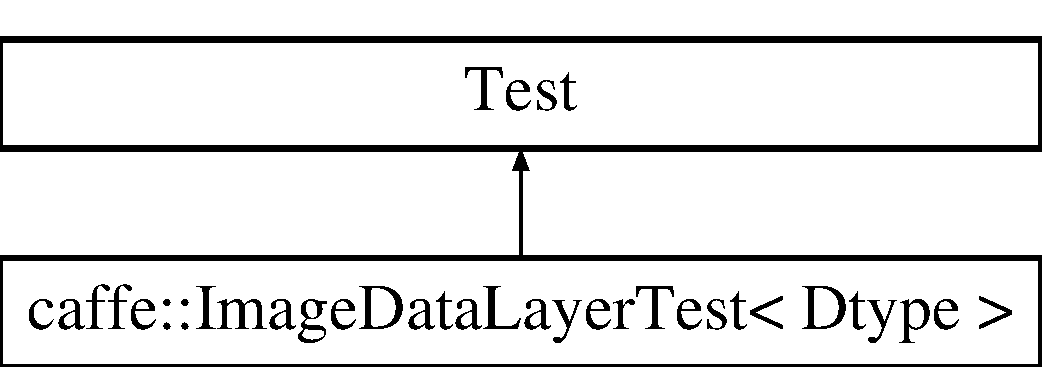
\includegraphics[height=2.000000cm]{classcaffe_1_1_image_data_layer_test}
\end{center}
\end{figure}
\subsection*{Protected Member Functions}
\begin{DoxyCompactItemize}
\item 
\hyperlink{classcaffe_1_1_image_data_layer_test_af1d71a610e1c3b64fb83c8104e7b3251}{Image\+Data\+Layer\+Test} ()
\item 
virtual void \hyperlink{classcaffe_1_1_image_data_layer_test_a912500336c22c500a0f3da9e5d63b50c}{Set\+Up} ()
\item 
virtual \hyperlink{classcaffe_1_1_image_data_layer_test_a0e84bd1ec1abea04a22efde477f32739}{$\sim$\+Image\+Data\+Layer\+Test} ()
\end{DoxyCompactItemize}
\subsection*{Protected Attributes}
\begin{DoxyCompactItemize}
\item 
int \hyperlink{classcaffe_1_1_image_data_layer_test_a924f088ff064f4b906f55afb402dad96}{seed\+\_\+}
\item 
shared\+\_\+ptr$<$ string $>$ \hyperlink{classcaffe_1_1_image_data_layer_test_a88c92cbd5af9edcd0f0c3b0866b1a637}{filename\+\_\+}
\item 
\hyperlink{classcaffe_1_1_blob}{Blob}$<$ Dtype $>$ $\ast$const \hyperlink{classcaffe_1_1_image_data_layer_test_a6e19bc2019229f48d4c4144be5c45862}{blob\+\_\+top\+\_\+data\+\_\+}
\item 
\hyperlink{classcaffe_1_1_blob}{Blob}$<$ Dtype $>$ $\ast$const \hyperlink{classcaffe_1_1_image_data_layer_test_aa134584d35b9b3a7a8a6d3a124be3bc9}{blob\+\_\+top\+\_\+label\+\_\+}
\item 
vector$<$ \hyperlink{classcaffe_1_1_blob}{Blob}$<$ Dtype $>$ $\ast$ $>$ \hyperlink{classcaffe_1_1_image_data_layer_test_a79a6acfec89c11df35f53489d7ea5912}{blob\+\_\+bottom\+\_\+vec\+\_\+}
\item 
vector$<$ \hyperlink{classcaffe_1_1_blob}{Blob}$<$ Dtype $>$ $\ast$ $>$ \hyperlink{classcaffe_1_1_image_data_layer_test_a88ea0aa61835ea8c448c21938c39b75a}{blob\+\_\+top\+\_\+vec\+\_\+}
\end{DoxyCompactItemize}


\subsection{Constructor \& Destructor Documentation}
\hypertarget{classcaffe_1_1_image_data_layer_test_af1d71a610e1c3b64fb83c8104e7b3251}{\index{caffe\+::\+Image\+Data\+Layer\+Test@{caffe\+::\+Image\+Data\+Layer\+Test}!Image\+Data\+Layer\+Test@{Image\+Data\+Layer\+Test}}
\index{Image\+Data\+Layer\+Test@{Image\+Data\+Layer\+Test}!caffe\+::\+Image\+Data\+Layer\+Test@{caffe\+::\+Image\+Data\+Layer\+Test}}
\subsubsection[{Image\+Data\+Layer\+Test}]{\setlength{\rightskip}{0pt plus 5cm}template$<$typename Dtype $>$ {\bf caffe\+::\+Image\+Data\+Layer\+Test}$<$ Dtype $>$\+::{\bf Image\+Data\+Layer\+Test} (
\begin{DoxyParamCaption}
{}
\end{DoxyParamCaption}
)\hspace{0.3cm}{\ttfamily [inline]}, {\ttfamily [protected]}}}\label{classcaffe_1_1_image_data_layer_test_af1d71a610e1c3b64fb83c8104e7b3251}
\hypertarget{classcaffe_1_1_image_data_layer_test_a0e84bd1ec1abea04a22efde477f32739}{\index{caffe\+::\+Image\+Data\+Layer\+Test@{caffe\+::\+Image\+Data\+Layer\+Test}!````~Image\+Data\+Layer\+Test@{$\sim$\+Image\+Data\+Layer\+Test}}
\index{````~Image\+Data\+Layer\+Test@{$\sim$\+Image\+Data\+Layer\+Test}!caffe\+::\+Image\+Data\+Layer\+Test@{caffe\+::\+Image\+Data\+Layer\+Test}}
\subsubsection[{$\sim$\+Image\+Data\+Layer\+Test}]{\setlength{\rightskip}{0pt plus 5cm}template$<$typename Dtype $>$ virtual {\bf caffe\+::\+Image\+Data\+Layer\+Test}$<$ Dtype $>$\+::$\sim${\bf Image\+Data\+Layer\+Test} (
\begin{DoxyParamCaption}
{}
\end{DoxyParamCaption}
)\hspace{0.3cm}{\ttfamily [inline]}, {\ttfamily [protected]}, {\ttfamily [virtual]}}}\label{classcaffe_1_1_image_data_layer_test_a0e84bd1ec1abea04a22efde477f32739}


\subsection{Member Function Documentation}
\hypertarget{classcaffe_1_1_image_data_layer_test_a912500336c22c500a0f3da9e5d63b50c}{\index{caffe\+::\+Image\+Data\+Layer\+Test@{caffe\+::\+Image\+Data\+Layer\+Test}!Set\+Up@{Set\+Up}}
\index{Set\+Up@{Set\+Up}!caffe\+::\+Image\+Data\+Layer\+Test@{caffe\+::\+Image\+Data\+Layer\+Test}}
\subsubsection[{Set\+Up}]{\setlength{\rightskip}{0pt plus 5cm}template$<$typename Dtype $>$ virtual void {\bf caffe\+::\+Image\+Data\+Layer\+Test}$<$ Dtype $>$\+::Set\+Up (
\begin{DoxyParamCaption}
{}
\end{DoxyParamCaption}
)\hspace{0.3cm}{\ttfamily [inline]}, {\ttfamily [protected]}, {\ttfamily [virtual]}}}\label{classcaffe_1_1_image_data_layer_test_a912500336c22c500a0f3da9e5d63b50c}


\subsection{Member Data Documentation}
\hypertarget{classcaffe_1_1_image_data_layer_test_a79a6acfec89c11df35f53489d7ea5912}{\index{caffe\+::\+Image\+Data\+Layer\+Test@{caffe\+::\+Image\+Data\+Layer\+Test}!blob\+\_\+bottom\+\_\+vec\+\_\+@{blob\+\_\+bottom\+\_\+vec\+\_\+}}
\index{blob\+\_\+bottom\+\_\+vec\+\_\+@{blob\+\_\+bottom\+\_\+vec\+\_\+}!caffe\+::\+Image\+Data\+Layer\+Test@{caffe\+::\+Image\+Data\+Layer\+Test}}
\subsubsection[{blob\+\_\+bottom\+\_\+vec\+\_\+}]{\setlength{\rightskip}{0pt plus 5cm}template$<$typename Dtype $>$ vector$<${\bf Blob}$<$Dtype$>$$\ast$$>$ {\bf caffe\+::\+Image\+Data\+Layer\+Test}$<$ Dtype $>$\+::blob\+\_\+bottom\+\_\+vec\+\_\+\hspace{0.3cm}{\ttfamily [protected]}}}\label{classcaffe_1_1_image_data_layer_test_a79a6acfec89c11df35f53489d7ea5912}
\hypertarget{classcaffe_1_1_image_data_layer_test_a6e19bc2019229f48d4c4144be5c45862}{\index{caffe\+::\+Image\+Data\+Layer\+Test@{caffe\+::\+Image\+Data\+Layer\+Test}!blob\+\_\+top\+\_\+data\+\_\+@{blob\+\_\+top\+\_\+data\+\_\+}}
\index{blob\+\_\+top\+\_\+data\+\_\+@{blob\+\_\+top\+\_\+data\+\_\+}!caffe\+::\+Image\+Data\+Layer\+Test@{caffe\+::\+Image\+Data\+Layer\+Test}}
\subsubsection[{blob\+\_\+top\+\_\+data\+\_\+}]{\setlength{\rightskip}{0pt plus 5cm}template$<$typename Dtype $>$ {\bf Blob}$<$Dtype$>$$\ast$ const {\bf caffe\+::\+Image\+Data\+Layer\+Test}$<$ Dtype $>$\+::blob\+\_\+top\+\_\+data\+\_\+\hspace{0.3cm}{\ttfamily [protected]}}}\label{classcaffe_1_1_image_data_layer_test_a6e19bc2019229f48d4c4144be5c45862}
\hypertarget{classcaffe_1_1_image_data_layer_test_aa134584d35b9b3a7a8a6d3a124be3bc9}{\index{caffe\+::\+Image\+Data\+Layer\+Test@{caffe\+::\+Image\+Data\+Layer\+Test}!blob\+\_\+top\+\_\+label\+\_\+@{blob\+\_\+top\+\_\+label\+\_\+}}
\index{blob\+\_\+top\+\_\+label\+\_\+@{blob\+\_\+top\+\_\+label\+\_\+}!caffe\+::\+Image\+Data\+Layer\+Test@{caffe\+::\+Image\+Data\+Layer\+Test}}
\subsubsection[{blob\+\_\+top\+\_\+label\+\_\+}]{\setlength{\rightskip}{0pt plus 5cm}template$<$typename Dtype $>$ {\bf Blob}$<$Dtype$>$$\ast$ const {\bf caffe\+::\+Image\+Data\+Layer\+Test}$<$ Dtype $>$\+::blob\+\_\+top\+\_\+label\+\_\+\hspace{0.3cm}{\ttfamily [protected]}}}\label{classcaffe_1_1_image_data_layer_test_aa134584d35b9b3a7a8a6d3a124be3bc9}
\hypertarget{classcaffe_1_1_image_data_layer_test_a88ea0aa61835ea8c448c21938c39b75a}{\index{caffe\+::\+Image\+Data\+Layer\+Test@{caffe\+::\+Image\+Data\+Layer\+Test}!blob\+\_\+top\+\_\+vec\+\_\+@{blob\+\_\+top\+\_\+vec\+\_\+}}
\index{blob\+\_\+top\+\_\+vec\+\_\+@{blob\+\_\+top\+\_\+vec\+\_\+}!caffe\+::\+Image\+Data\+Layer\+Test@{caffe\+::\+Image\+Data\+Layer\+Test}}
\subsubsection[{blob\+\_\+top\+\_\+vec\+\_\+}]{\setlength{\rightskip}{0pt plus 5cm}template$<$typename Dtype $>$ vector$<${\bf Blob}$<$Dtype$>$$\ast$$>$ {\bf caffe\+::\+Image\+Data\+Layer\+Test}$<$ Dtype $>$\+::blob\+\_\+top\+\_\+vec\+\_\+\hspace{0.3cm}{\ttfamily [protected]}}}\label{classcaffe_1_1_image_data_layer_test_a88ea0aa61835ea8c448c21938c39b75a}
\hypertarget{classcaffe_1_1_image_data_layer_test_a88c92cbd5af9edcd0f0c3b0866b1a637}{\index{caffe\+::\+Image\+Data\+Layer\+Test@{caffe\+::\+Image\+Data\+Layer\+Test}!filename\+\_\+@{filename\+\_\+}}
\index{filename\+\_\+@{filename\+\_\+}!caffe\+::\+Image\+Data\+Layer\+Test@{caffe\+::\+Image\+Data\+Layer\+Test}}
\subsubsection[{filename\+\_\+}]{\setlength{\rightskip}{0pt plus 5cm}template$<$typename Dtype $>$ shared\+\_\+ptr$<$string$>$ {\bf caffe\+::\+Image\+Data\+Layer\+Test}$<$ Dtype $>$\+::filename\+\_\+\hspace{0.3cm}{\ttfamily [protected]}}}\label{classcaffe_1_1_image_data_layer_test_a88c92cbd5af9edcd0f0c3b0866b1a637}
\hypertarget{classcaffe_1_1_image_data_layer_test_a924f088ff064f4b906f55afb402dad96}{\index{caffe\+::\+Image\+Data\+Layer\+Test@{caffe\+::\+Image\+Data\+Layer\+Test}!seed\+\_\+@{seed\+\_\+}}
\index{seed\+\_\+@{seed\+\_\+}!caffe\+::\+Image\+Data\+Layer\+Test@{caffe\+::\+Image\+Data\+Layer\+Test}}
\subsubsection[{seed\+\_\+}]{\setlength{\rightskip}{0pt plus 5cm}template$<$typename Dtype $>$ int {\bf caffe\+::\+Image\+Data\+Layer\+Test}$<$ Dtype $>$\+::seed\+\_\+\hspace{0.3cm}{\ttfamily [protected]}}}\label{classcaffe_1_1_image_data_layer_test_a924f088ff064f4b906f55afb402dad96}


The documentation for this class was generated from the following file\+:\begin{DoxyCompactItemize}
\item 
src/caffe/test/\hyperlink{test__image__data__layer_8cpp}{test\+\_\+image\+\_\+data\+\_\+layer.\+cpp}\end{DoxyCompactItemize}

\hypertarget{classcaffe_1_1_infogain_loss_layer}{\section{caffe\+:\+:Infogain\+Loss\+Layer$<$ Dtype $>$ Class Template Reference}
\label{classcaffe_1_1_infogain_loss_layer}\index{caffe\+::\+Infogain\+Loss\+Layer$<$ Dtype $>$@{caffe\+::\+Infogain\+Loss\+Layer$<$ Dtype $>$}}
}


{\ttfamily \#include $<$vision\+\_\+layers.\+hpp$>$}

Inheritance diagram for caffe\+:\+:Infogain\+Loss\+Layer$<$ Dtype $>$\+:\begin{figure}[H]
\begin{center}
\leavevmode
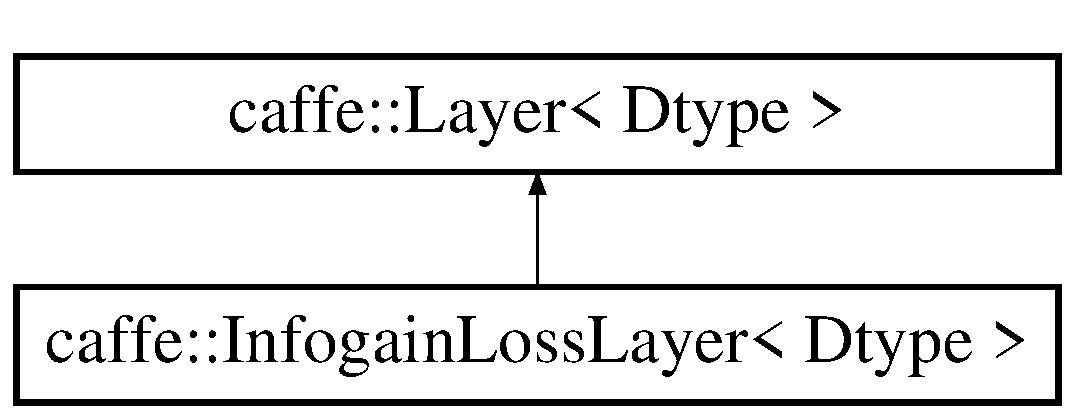
\includegraphics[height=2.000000cm]{classcaffe_1_1_infogain_loss_layer}
\end{center}
\end{figure}
\subsection*{Public Member Functions}
\begin{DoxyCompactItemize}
\item 
\hyperlink{classcaffe_1_1_infogain_loss_layer_ac2269ba8dc7d18fa8fab90ea9f295784}{Infogain\+Loss\+Layer} (const Layer\+Parameter \&param)
\item 
virtual void \hyperlink{classcaffe_1_1_infogain_loss_layer_a22a1826f68b20911bcd2941e2284fd9e}{Set\+Up} (const vector$<$ \hyperlink{classcaffe_1_1_blob}{Blob}$<$ Dtype $>$ $\ast$ $>$ \&bottom, vector$<$ \hyperlink{classcaffe_1_1_blob}{Blob}$<$ Dtype $>$ $\ast$ $>$ $\ast$top)
\end{DoxyCompactItemize}
\subsection*{Protected Member Functions}
\begin{DoxyCompactItemize}
\item 
virtual Dtype \hyperlink{classcaffe_1_1_infogain_loss_layer_ab5a8e36c29baa36e34b81a06d04043b6}{Forward\+\_\+cpu} (const vector$<$ \hyperlink{classcaffe_1_1_blob}{Blob}$<$ Dtype $>$ $\ast$ $>$ \&bottom, vector$<$ \hyperlink{classcaffe_1_1_blob}{Blob}$<$ Dtype $>$ $\ast$ $>$ $\ast$top)
\item 
virtual void \hyperlink{classcaffe_1_1_infogain_loss_layer_a3fea9231eb9c3f1cd2f3989c54e475a8}{Backward\+\_\+cpu} (const vector$<$ \hyperlink{classcaffe_1_1_blob}{Blob}$<$ Dtype $>$ $\ast$ $>$ \&top, const bool propagate\+\_\+down, vector$<$ \hyperlink{classcaffe_1_1_blob}{Blob}$<$ Dtype $>$ $\ast$ $>$ $\ast$bottom)
\end{DoxyCompactItemize}
\subsection*{Protected Attributes}
\begin{DoxyCompactItemize}
\item 
\hyperlink{classcaffe_1_1_blob}{Blob}$<$ Dtype $>$ \hyperlink{classcaffe_1_1_infogain_loss_layer_a2d9ffe8c64b096042cc75fced30dcaca}{infogain\+\_\+}
\end{DoxyCompactItemize}


\subsection{Constructor \& Destructor Documentation}
\hypertarget{classcaffe_1_1_infogain_loss_layer_ac2269ba8dc7d18fa8fab90ea9f295784}{\index{caffe\+::\+Infogain\+Loss\+Layer@{caffe\+::\+Infogain\+Loss\+Layer}!Infogain\+Loss\+Layer@{Infogain\+Loss\+Layer}}
\index{Infogain\+Loss\+Layer@{Infogain\+Loss\+Layer}!caffe\+::\+Infogain\+Loss\+Layer@{caffe\+::\+Infogain\+Loss\+Layer}}
\subsubsection[{Infogain\+Loss\+Layer}]{\setlength{\rightskip}{0pt plus 5cm}template$<$typename Dtype $>$ {\bf caffe\+::\+Infogain\+Loss\+Layer}$<$ Dtype $>$\+::{\bf Infogain\+Loss\+Layer} (
\begin{DoxyParamCaption}
\item[{const Layer\+Parameter \&}]{param}
\end{DoxyParamCaption}
)\hspace{0.3cm}{\ttfamily [inline]}, {\ttfamily [explicit]}}}\label{classcaffe_1_1_infogain_loss_layer_ac2269ba8dc7d18fa8fab90ea9f295784}


\subsection{Member Function Documentation}
\hypertarget{classcaffe_1_1_infogain_loss_layer_a3fea9231eb9c3f1cd2f3989c54e475a8}{\index{caffe\+::\+Infogain\+Loss\+Layer@{caffe\+::\+Infogain\+Loss\+Layer}!Backward\+\_\+cpu@{Backward\+\_\+cpu}}
\index{Backward\+\_\+cpu@{Backward\+\_\+cpu}!caffe\+::\+Infogain\+Loss\+Layer@{caffe\+::\+Infogain\+Loss\+Layer}}
\subsubsection[{Backward\+\_\+cpu}]{\setlength{\rightskip}{0pt plus 5cm}template$<$typename Dtype $>$ void {\bf caffe\+::\+Infogain\+Loss\+Layer}$<$ Dtype $>$\+::Backward\+\_\+cpu (
\begin{DoxyParamCaption}
\item[{const vector$<$ {\bf Blob}$<$ Dtype $>$ $\ast$ $>$ \&}]{top, }
\item[{const bool}]{propagate\+\_\+down, }
\item[{vector$<$ {\bf Blob}$<$ Dtype $>$ $\ast$ $>$ $\ast$}]{bottom}
\end{DoxyParamCaption}
)\hspace{0.3cm}{\ttfamily [protected]}, {\ttfamily [virtual]}}}\label{classcaffe_1_1_infogain_loss_layer_a3fea9231eb9c3f1cd2f3989c54e475a8}


Implements \hyperlink{classcaffe_1_1_layer_ac2d82011d076237c67997f63e7ee4b80}{caffe\+::\+Layer$<$ Dtype $>$}.

\hypertarget{classcaffe_1_1_infogain_loss_layer_ab5a8e36c29baa36e34b81a06d04043b6}{\index{caffe\+::\+Infogain\+Loss\+Layer@{caffe\+::\+Infogain\+Loss\+Layer}!Forward\+\_\+cpu@{Forward\+\_\+cpu}}
\index{Forward\+\_\+cpu@{Forward\+\_\+cpu}!caffe\+::\+Infogain\+Loss\+Layer@{caffe\+::\+Infogain\+Loss\+Layer}}
\subsubsection[{Forward\+\_\+cpu}]{\setlength{\rightskip}{0pt plus 5cm}template$<$typename Dtype $>$ Dtype {\bf caffe\+::\+Infogain\+Loss\+Layer}$<$ Dtype $>$\+::Forward\+\_\+cpu (
\begin{DoxyParamCaption}
\item[{const vector$<$ {\bf Blob}$<$ Dtype $>$ $\ast$ $>$ \&}]{bottom, }
\item[{vector$<$ {\bf Blob}$<$ Dtype $>$ $\ast$ $>$ $\ast$}]{top}
\end{DoxyParamCaption}
)\hspace{0.3cm}{\ttfamily [protected]}, {\ttfamily [virtual]}}}\label{classcaffe_1_1_infogain_loss_layer_ab5a8e36c29baa36e34b81a06d04043b6}


Implements \hyperlink{classcaffe_1_1_layer_a8f7f61da3b8b3ca7f2394dee33873353}{caffe\+::\+Layer$<$ Dtype $>$}.

\hypertarget{classcaffe_1_1_infogain_loss_layer_a22a1826f68b20911bcd2941e2284fd9e}{\index{caffe\+::\+Infogain\+Loss\+Layer@{caffe\+::\+Infogain\+Loss\+Layer}!Set\+Up@{Set\+Up}}
\index{Set\+Up@{Set\+Up}!caffe\+::\+Infogain\+Loss\+Layer@{caffe\+::\+Infogain\+Loss\+Layer}}
\subsubsection[{Set\+Up}]{\setlength{\rightskip}{0pt plus 5cm}template$<$typename Dtype $>$ void {\bf caffe\+::\+Infogain\+Loss\+Layer}$<$ Dtype $>$\+::Set\+Up (
\begin{DoxyParamCaption}
\item[{const vector$<$ {\bf Blob}$<$ Dtype $>$ $\ast$ $>$ \&}]{bottom, }
\item[{vector$<$ {\bf Blob}$<$ Dtype $>$ $\ast$ $>$ $\ast$}]{top}
\end{DoxyParamCaption}
)\hspace{0.3cm}{\ttfamily [virtual]}}}\label{classcaffe_1_1_infogain_loss_layer_a22a1826f68b20911bcd2941e2284fd9e}


Implements \hyperlink{classcaffe_1_1_layer_abd13c6489c13953b4fbcfcf6880835d0}{caffe\+::\+Layer$<$ Dtype $>$}.



\subsection{Member Data Documentation}
\hypertarget{classcaffe_1_1_infogain_loss_layer_a2d9ffe8c64b096042cc75fced30dcaca}{\index{caffe\+::\+Infogain\+Loss\+Layer@{caffe\+::\+Infogain\+Loss\+Layer}!infogain\+\_\+@{infogain\+\_\+}}
\index{infogain\+\_\+@{infogain\+\_\+}!caffe\+::\+Infogain\+Loss\+Layer@{caffe\+::\+Infogain\+Loss\+Layer}}
\subsubsection[{infogain\+\_\+}]{\setlength{\rightskip}{0pt plus 5cm}template$<$typename Dtype $>$ {\bf Blob}$<$Dtype$>$ {\bf caffe\+::\+Infogain\+Loss\+Layer}$<$ Dtype $>$\+::infogain\+\_\+\hspace{0.3cm}{\ttfamily [protected]}}}\label{classcaffe_1_1_infogain_loss_layer_a2d9ffe8c64b096042cc75fced30dcaca}


The documentation for this class was generated from the following files\+:\begin{DoxyCompactItemize}
\item 
include/caffe/\hyperlink{vision__layers_8hpp}{vision\+\_\+layers.\+hpp}\item 
src/caffe/layers/\hyperlink{loss__layer_8cpp}{loss\+\_\+layer.\+cpp}\end{DoxyCompactItemize}

\hypertarget{classcaffe_1_1_inner_product_layer}{\section{caffe\+:\+:Inner\+Product\+Layer$<$ Dtype $>$ Class Template Reference}
\label{classcaffe_1_1_inner_product_layer}\index{caffe\+::\+Inner\+Product\+Layer$<$ Dtype $>$@{caffe\+::\+Inner\+Product\+Layer$<$ Dtype $>$}}
}


{\ttfamily \#include $<$vision\+\_\+layers.\+hpp$>$}

Inheritance diagram for caffe\+:\+:Inner\+Product\+Layer$<$ Dtype $>$\+:\begin{figure}[H]
\begin{center}
\leavevmode
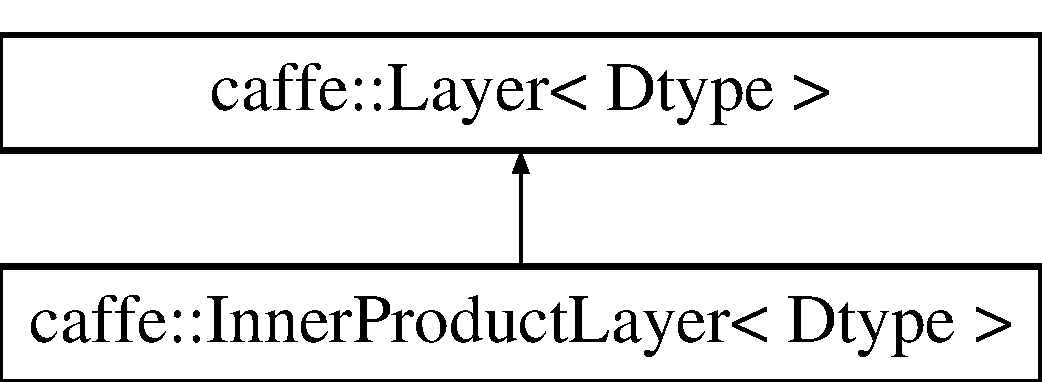
\includegraphics[height=2.000000cm]{classcaffe_1_1_inner_product_layer}
\end{center}
\end{figure}
\subsection*{Public Member Functions}
\begin{DoxyCompactItemize}
\item 
\hyperlink{classcaffe_1_1_inner_product_layer_a997e3c54ed0414ebcd8eec13f083af07}{Inner\+Product\+Layer} (const Layer\+Parameter \&param)
\item 
virtual void \hyperlink{classcaffe_1_1_inner_product_layer_a3e95f827d46406c96575d8852b4d68fe}{Set\+Up} (const vector$<$ \hyperlink{classcaffe_1_1_blob}{Blob}$<$ Dtype $>$ $\ast$ $>$ \&bottom, vector$<$ \hyperlink{classcaffe_1_1_blob}{Blob}$<$ Dtype $>$ $\ast$ $>$ $\ast$top)
\end{DoxyCompactItemize}
\subsection*{Protected Member Functions}
\begin{DoxyCompactItemize}
\item 
virtual Dtype \hyperlink{classcaffe_1_1_inner_product_layer_afa97ce030d4fec47cca1bd758bc446f3}{Forward\+\_\+cpu} (const vector$<$ \hyperlink{classcaffe_1_1_blob}{Blob}$<$ Dtype $>$ $\ast$ $>$ \&bottom, vector$<$ \hyperlink{classcaffe_1_1_blob}{Blob}$<$ Dtype $>$ $\ast$ $>$ $\ast$top)
\item 
virtual Dtype \hyperlink{classcaffe_1_1_inner_product_layer_a309180d8bbea21a281de52f3465ea786}{Forward\+\_\+gpu} (const vector$<$ \hyperlink{classcaffe_1_1_blob}{Blob}$<$ Dtype $>$ $\ast$ $>$ \&bottom, vector$<$ \hyperlink{classcaffe_1_1_blob}{Blob}$<$ Dtype $>$ $\ast$ $>$ $\ast$top)
\item 
virtual void \hyperlink{classcaffe_1_1_inner_product_layer_ab4f9892f3be7aef5d98777bca2dd8598}{Backward\+\_\+cpu} (const vector$<$ \hyperlink{classcaffe_1_1_blob}{Blob}$<$ Dtype $>$ $\ast$ $>$ \&top, const bool propagate\+\_\+down, vector$<$ \hyperlink{classcaffe_1_1_blob}{Blob}$<$ Dtype $>$ $\ast$ $>$ $\ast$bottom)
\item 
virtual void \hyperlink{classcaffe_1_1_inner_product_layer_a67252d33aaf6efb6ef5ce2e450cc4ca8}{Backward\+\_\+gpu} (const vector$<$ \hyperlink{classcaffe_1_1_blob}{Blob}$<$ Dtype $>$ $\ast$ $>$ \&top, const bool propagate\+\_\+down, vector$<$ \hyperlink{classcaffe_1_1_blob}{Blob}$<$ Dtype $>$ $\ast$ $>$ $\ast$bottom)
\end{DoxyCompactItemize}
\subsection*{Protected Attributes}
\begin{DoxyCompactItemize}
\item 
int \hyperlink{classcaffe_1_1_inner_product_layer_a7cfcde40b118c74a0e85aa3b58e8aa07}{M\+\_\+}
\item 
int \hyperlink{classcaffe_1_1_inner_product_layer_ad5a55ef3cb96a332977930cfaa700c66}{K\+\_\+}
\item 
int \hyperlink{classcaffe_1_1_inner_product_layer_a863f699772bf8b8d978d6ec8bca42463}{N\+\_\+}
\item 
bool \hyperlink{classcaffe_1_1_inner_product_layer_a7193d161e30f35b3f6d23293480eb683}{bias\+\_\+term\+\_\+}
\item 
shared\+\_\+ptr$<$ \hyperlink{classcaffe_1_1_synced_memory}{Synced\+Memory} $>$ \hyperlink{classcaffe_1_1_inner_product_layer_a2d7ebfa9183f4e4bdf9546965c3cc0a8}{bias\+\_\+multiplier\+\_\+}
\end{DoxyCompactItemize}


\subsection{Constructor \& Destructor Documentation}
\hypertarget{classcaffe_1_1_inner_product_layer_a997e3c54ed0414ebcd8eec13f083af07}{\index{caffe\+::\+Inner\+Product\+Layer@{caffe\+::\+Inner\+Product\+Layer}!Inner\+Product\+Layer@{Inner\+Product\+Layer}}
\index{Inner\+Product\+Layer@{Inner\+Product\+Layer}!caffe\+::\+Inner\+Product\+Layer@{caffe\+::\+Inner\+Product\+Layer}}
\subsubsection[{Inner\+Product\+Layer}]{\setlength{\rightskip}{0pt plus 5cm}template$<$typename Dtype $>$ {\bf caffe\+::\+Inner\+Product\+Layer}$<$ Dtype $>$\+::{\bf Inner\+Product\+Layer} (
\begin{DoxyParamCaption}
\item[{const Layer\+Parameter \&}]{param}
\end{DoxyParamCaption}
)\hspace{0.3cm}{\ttfamily [inline]}, {\ttfamily [explicit]}}}\label{classcaffe_1_1_inner_product_layer_a997e3c54ed0414ebcd8eec13f083af07}


\subsection{Member Function Documentation}
\hypertarget{classcaffe_1_1_inner_product_layer_ab4f9892f3be7aef5d98777bca2dd8598}{\index{caffe\+::\+Inner\+Product\+Layer@{caffe\+::\+Inner\+Product\+Layer}!Backward\+\_\+cpu@{Backward\+\_\+cpu}}
\index{Backward\+\_\+cpu@{Backward\+\_\+cpu}!caffe\+::\+Inner\+Product\+Layer@{caffe\+::\+Inner\+Product\+Layer}}
\subsubsection[{Backward\+\_\+cpu}]{\setlength{\rightskip}{0pt plus 5cm}template$<$typename Dtype $>$ void {\bf caffe\+::\+Inner\+Product\+Layer}$<$ Dtype $>$\+::Backward\+\_\+cpu (
\begin{DoxyParamCaption}
\item[{const vector$<$ {\bf Blob}$<$ Dtype $>$ $\ast$ $>$ \&}]{top, }
\item[{const bool}]{propagate\+\_\+down, }
\item[{vector$<$ {\bf Blob}$<$ Dtype $>$ $\ast$ $>$ $\ast$}]{bottom}
\end{DoxyParamCaption}
)\hspace{0.3cm}{\ttfamily [protected]}, {\ttfamily [virtual]}}}\label{classcaffe_1_1_inner_product_layer_ab4f9892f3be7aef5d98777bca2dd8598}


Implements \hyperlink{classcaffe_1_1_layer_ac2d82011d076237c67997f63e7ee4b80}{caffe\+::\+Layer$<$ Dtype $>$}.

\hypertarget{classcaffe_1_1_inner_product_layer_a67252d33aaf6efb6ef5ce2e450cc4ca8}{\index{caffe\+::\+Inner\+Product\+Layer@{caffe\+::\+Inner\+Product\+Layer}!Backward\+\_\+gpu@{Backward\+\_\+gpu}}
\index{Backward\+\_\+gpu@{Backward\+\_\+gpu}!caffe\+::\+Inner\+Product\+Layer@{caffe\+::\+Inner\+Product\+Layer}}
\subsubsection[{Backward\+\_\+gpu}]{\setlength{\rightskip}{0pt plus 5cm}template$<$typename Dtype $>$ void {\bf caffe\+::\+Inner\+Product\+Layer}$<$ Dtype $>$\+::Backward\+\_\+gpu (
\begin{DoxyParamCaption}
\item[{const vector$<$ {\bf Blob}$<$ Dtype $>$ $\ast$ $>$ \&}]{top, }
\item[{const bool}]{propagate\+\_\+down, }
\item[{vector$<$ {\bf Blob}$<$ Dtype $>$ $\ast$ $>$ $\ast$}]{bottom}
\end{DoxyParamCaption}
)\hspace{0.3cm}{\ttfamily [protected]}, {\ttfamily [virtual]}}}\label{classcaffe_1_1_inner_product_layer_a67252d33aaf6efb6ef5ce2e450cc4ca8}


Reimplemented from \hyperlink{classcaffe_1_1_layer_adf07ffe1f22d2fd2b1b0ff475ef5a64b}{caffe\+::\+Layer$<$ Dtype $>$}.

\hypertarget{classcaffe_1_1_inner_product_layer_afa97ce030d4fec47cca1bd758bc446f3}{\index{caffe\+::\+Inner\+Product\+Layer@{caffe\+::\+Inner\+Product\+Layer}!Forward\+\_\+cpu@{Forward\+\_\+cpu}}
\index{Forward\+\_\+cpu@{Forward\+\_\+cpu}!caffe\+::\+Inner\+Product\+Layer@{caffe\+::\+Inner\+Product\+Layer}}
\subsubsection[{Forward\+\_\+cpu}]{\setlength{\rightskip}{0pt plus 5cm}template$<$typename Dtype $>$ Dtype {\bf caffe\+::\+Inner\+Product\+Layer}$<$ Dtype $>$\+::Forward\+\_\+cpu (
\begin{DoxyParamCaption}
\item[{const vector$<$ {\bf Blob}$<$ Dtype $>$ $\ast$ $>$ \&}]{bottom, }
\item[{vector$<$ {\bf Blob}$<$ Dtype $>$ $\ast$ $>$ $\ast$}]{top}
\end{DoxyParamCaption}
)\hspace{0.3cm}{\ttfamily [protected]}, {\ttfamily [virtual]}}}\label{classcaffe_1_1_inner_product_layer_afa97ce030d4fec47cca1bd758bc446f3}


Implements \hyperlink{classcaffe_1_1_layer_a8f7f61da3b8b3ca7f2394dee33873353}{caffe\+::\+Layer$<$ Dtype $>$}.

\hypertarget{classcaffe_1_1_inner_product_layer_a309180d8bbea21a281de52f3465ea786}{\index{caffe\+::\+Inner\+Product\+Layer@{caffe\+::\+Inner\+Product\+Layer}!Forward\+\_\+gpu@{Forward\+\_\+gpu}}
\index{Forward\+\_\+gpu@{Forward\+\_\+gpu}!caffe\+::\+Inner\+Product\+Layer@{caffe\+::\+Inner\+Product\+Layer}}
\subsubsection[{Forward\+\_\+gpu}]{\setlength{\rightskip}{0pt plus 5cm}template$<$typename Dtype $>$ Dtype {\bf caffe\+::\+Inner\+Product\+Layer}$<$ Dtype $>$\+::Forward\+\_\+gpu (
\begin{DoxyParamCaption}
\item[{const vector$<$ {\bf Blob}$<$ Dtype $>$ $\ast$ $>$ \&}]{bottom, }
\item[{vector$<$ {\bf Blob}$<$ Dtype $>$ $\ast$ $>$ $\ast$}]{top}
\end{DoxyParamCaption}
)\hspace{0.3cm}{\ttfamily [protected]}, {\ttfamily [virtual]}}}\label{classcaffe_1_1_inner_product_layer_a309180d8bbea21a281de52f3465ea786}


Reimplemented from \hyperlink{classcaffe_1_1_layer_a2d78dbf5d8bc36928bd8f6fcfbafbcef}{caffe\+::\+Layer$<$ Dtype $>$}.

\hypertarget{classcaffe_1_1_inner_product_layer_a3e95f827d46406c96575d8852b4d68fe}{\index{caffe\+::\+Inner\+Product\+Layer@{caffe\+::\+Inner\+Product\+Layer}!Set\+Up@{Set\+Up}}
\index{Set\+Up@{Set\+Up}!caffe\+::\+Inner\+Product\+Layer@{caffe\+::\+Inner\+Product\+Layer}}
\subsubsection[{Set\+Up}]{\setlength{\rightskip}{0pt plus 5cm}template$<$typename Dtype $>$ void {\bf caffe\+::\+Inner\+Product\+Layer}$<$ Dtype $>$\+::Set\+Up (
\begin{DoxyParamCaption}
\item[{const vector$<$ {\bf Blob}$<$ Dtype $>$ $\ast$ $>$ \&}]{bottom, }
\item[{vector$<$ {\bf Blob}$<$ Dtype $>$ $\ast$ $>$ $\ast$}]{top}
\end{DoxyParamCaption}
)\hspace{0.3cm}{\ttfamily [virtual]}}}\label{classcaffe_1_1_inner_product_layer_a3e95f827d46406c96575d8852b4d68fe}


Implements \hyperlink{classcaffe_1_1_layer_abd13c6489c13953b4fbcfcf6880835d0}{caffe\+::\+Layer$<$ Dtype $>$}.



\subsection{Member Data Documentation}
\hypertarget{classcaffe_1_1_inner_product_layer_a2d7ebfa9183f4e4bdf9546965c3cc0a8}{\index{caffe\+::\+Inner\+Product\+Layer@{caffe\+::\+Inner\+Product\+Layer}!bias\+\_\+multiplier\+\_\+@{bias\+\_\+multiplier\+\_\+}}
\index{bias\+\_\+multiplier\+\_\+@{bias\+\_\+multiplier\+\_\+}!caffe\+::\+Inner\+Product\+Layer@{caffe\+::\+Inner\+Product\+Layer}}
\subsubsection[{bias\+\_\+multiplier\+\_\+}]{\setlength{\rightskip}{0pt plus 5cm}template$<$typename Dtype $>$ shared\+\_\+ptr$<${\bf Synced\+Memory}$>$ {\bf caffe\+::\+Inner\+Product\+Layer}$<$ Dtype $>$\+::bias\+\_\+multiplier\+\_\+\hspace{0.3cm}{\ttfamily [protected]}}}\label{classcaffe_1_1_inner_product_layer_a2d7ebfa9183f4e4bdf9546965c3cc0a8}
\hypertarget{classcaffe_1_1_inner_product_layer_a7193d161e30f35b3f6d23293480eb683}{\index{caffe\+::\+Inner\+Product\+Layer@{caffe\+::\+Inner\+Product\+Layer}!bias\+\_\+term\+\_\+@{bias\+\_\+term\+\_\+}}
\index{bias\+\_\+term\+\_\+@{bias\+\_\+term\+\_\+}!caffe\+::\+Inner\+Product\+Layer@{caffe\+::\+Inner\+Product\+Layer}}
\subsubsection[{bias\+\_\+term\+\_\+}]{\setlength{\rightskip}{0pt plus 5cm}template$<$typename Dtype $>$ bool {\bf caffe\+::\+Inner\+Product\+Layer}$<$ Dtype $>$\+::bias\+\_\+term\+\_\+\hspace{0.3cm}{\ttfamily [protected]}}}\label{classcaffe_1_1_inner_product_layer_a7193d161e30f35b3f6d23293480eb683}
\hypertarget{classcaffe_1_1_inner_product_layer_ad5a55ef3cb96a332977930cfaa700c66}{\index{caffe\+::\+Inner\+Product\+Layer@{caffe\+::\+Inner\+Product\+Layer}!K\+\_\+@{K\+\_\+}}
\index{K\+\_\+@{K\+\_\+}!caffe\+::\+Inner\+Product\+Layer@{caffe\+::\+Inner\+Product\+Layer}}
\subsubsection[{K\+\_\+}]{\setlength{\rightskip}{0pt plus 5cm}template$<$typename Dtype $>$ int {\bf caffe\+::\+Inner\+Product\+Layer}$<$ Dtype $>$\+::K\+\_\+\hspace{0.3cm}{\ttfamily [protected]}}}\label{classcaffe_1_1_inner_product_layer_ad5a55ef3cb96a332977930cfaa700c66}
\hypertarget{classcaffe_1_1_inner_product_layer_a7cfcde40b118c74a0e85aa3b58e8aa07}{\index{caffe\+::\+Inner\+Product\+Layer@{caffe\+::\+Inner\+Product\+Layer}!M\+\_\+@{M\+\_\+}}
\index{M\+\_\+@{M\+\_\+}!caffe\+::\+Inner\+Product\+Layer@{caffe\+::\+Inner\+Product\+Layer}}
\subsubsection[{M\+\_\+}]{\setlength{\rightskip}{0pt plus 5cm}template$<$typename Dtype $>$ int {\bf caffe\+::\+Inner\+Product\+Layer}$<$ Dtype $>$\+::M\+\_\+\hspace{0.3cm}{\ttfamily [protected]}}}\label{classcaffe_1_1_inner_product_layer_a7cfcde40b118c74a0e85aa3b58e8aa07}
\hypertarget{classcaffe_1_1_inner_product_layer_a863f699772bf8b8d978d6ec8bca42463}{\index{caffe\+::\+Inner\+Product\+Layer@{caffe\+::\+Inner\+Product\+Layer}!N\+\_\+@{N\+\_\+}}
\index{N\+\_\+@{N\+\_\+}!caffe\+::\+Inner\+Product\+Layer@{caffe\+::\+Inner\+Product\+Layer}}
\subsubsection[{N\+\_\+}]{\setlength{\rightskip}{0pt plus 5cm}template$<$typename Dtype $>$ int {\bf caffe\+::\+Inner\+Product\+Layer}$<$ Dtype $>$\+::N\+\_\+\hspace{0.3cm}{\ttfamily [protected]}}}\label{classcaffe_1_1_inner_product_layer_a863f699772bf8b8d978d6ec8bca42463}


The documentation for this class was generated from the following files\+:\begin{DoxyCompactItemize}
\item 
include/caffe/\hyperlink{vision__layers_8hpp}{vision\+\_\+layers.\+hpp}\item 
src/caffe/layers/\hyperlink{inner__product__layer_8cpp}{inner\+\_\+product\+\_\+layer.\+cpp}\item 
src/caffe/layers/\hyperlink{inner__product__layer_8cu}{inner\+\_\+product\+\_\+layer.\+cu}\end{DoxyCompactItemize}

\hypertarget{classcaffe_1_1_inner_product_layer_test}{\section{caffe\+:\+:Inner\+Product\+Layer\+Test$<$ Dtype $>$ Class Template Reference}
\label{classcaffe_1_1_inner_product_layer_test}\index{caffe\+::\+Inner\+Product\+Layer\+Test$<$ Dtype $>$@{caffe\+::\+Inner\+Product\+Layer\+Test$<$ Dtype $>$}}
}
Inheritance diagram for caffe\+:\+:Inner\+Product\+Layer\+Test$<$ Dtype $>$\+:\begin{figure}[H]
\begin{center}
\leavevmode
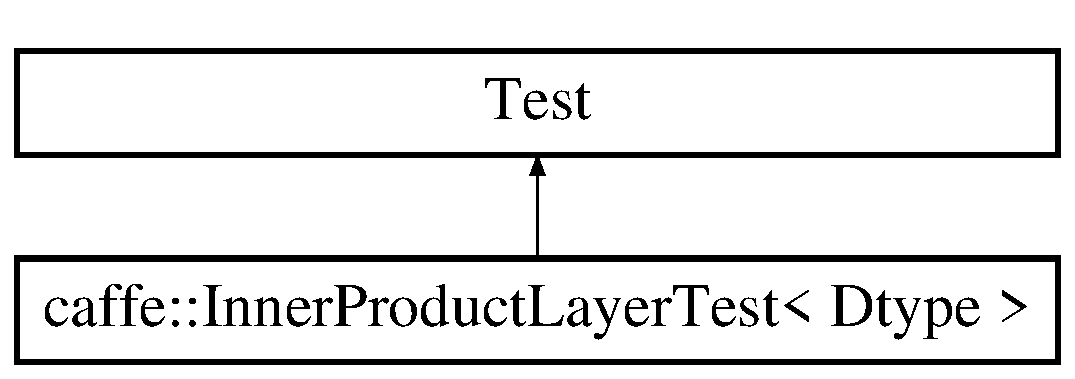
\includegraphics[height=2.000000cm]{classcaffe_1_1_inner_product_layer_test}
\end{center}
\end{figure}
\subsection*{Protected Member Functions}
\begin{DoxyCompactItemize}
\item 
\hyperlink{classcaffe_1_1_inner_product_layer_test_a96449bd1edf94bf783c3de331e967f9f}{Inner\+Product\+Layer\+Test} ()
\item 
virtual \hyperlink{classcaffe_1_1_inner_product_layer_test_a6755035389ffdf024d08e73bc870be60}{$\sim$\+Inner\+Product\+Layer\+Test} ()
\end{DoxyCompactItemize}
\subsection*{Protected Attributes}
\begin{DoxyCompactItemize}
\item 
\hyperlink{classcaffe_1_1_blob}{Blob}$<$ Dtype $>$ $\ast$const \hyperlink{classcaffe_1_1_inner_product_layer_test_adfa9bbdc3882fe32e7f73a776cf9baba}{blob\+\_\+bottom\+\_\+}
\item 
\hyperlink{classcaffe_1_1_blob}{Blob}$<$ Dtype $>$ $\ast$const \hyperlink{classcaffe_1_1_inner_product_layer_test_aba9a6f499c414653250a4cb9e81e0e70}{blob\+\_\+top\+\_\+}
\item 
vector$<$ \hyperlink{classcaffe_1_1_blob}{Blob}$<$ Dtype $>$ $\ast$ $>$ \hyperlink{classcaffe_1_1_inner_product_layer_test_acf2d5e26939568693b5fe360ce630d84}{blob\+\_\+bottom\+\_\+vec\+\_\+}
\item 
vector$<$ \hyperlink{classcaffe_1_1_blob}{Blob}$<$ Dtype $>$ $\ast$ $>$ \hyperlink{classcaffe_1_1_inner_product_layer_test_ac403f0c52fd366423da30010391c270e}{blob\+\_\+top\+\_\+vec\+\_\+}
\end{DoxyCompactItemize}


\subsection{Constructor \& Destructor Documentation}
\hypertarget{classcaffe_1_1_inner_product_layer_test_a96449bd1edf94bf783c3de331e967f9f}{\index{caffe\+::\+Inner\+Product\+Layer\+Test@{caffe\+::\+Inner\+Product\+Layer\+Test}!Inner\+Product\+Layer\+Test@{Inner\+Product\+Layer\+Test}}
\index{Inner\+Product\+Layer\+Test@{Inner\+Product\+Layer\+Test}!caffe\+::\+Inner\+Product\+Layer\+Test@{caffe\+::\+Inner\+Product\+Layer\+Test}}
\subsubsection[{Inner\+Product\+Layer\+Test}]{\setlength{\rightskip}{0pt plus 5cm}template$<$typename Dtype $>$ {\bf caffe\+::\+Inner\+Product\+Layer\+Test}$<$ Dtype $>$\+::{\bf Inner\+Product\+Layer\+Test} (
\begin{DoxyParamCaption}
{}
\end{DoxyParamCaption}
)\hspace{0.3cm}{\ttfamily [inline]}, {\ttfamily [protected]}}}\label{classcaffe_1_1_inner_product_layer_test_a96449bd1edf94bf783c3de331e967f9f}
\hypertarget{classcaffe_1_1_inner_product_layer_test_a6755035389ffdf024d08e73bc870be60}{\index{caffe\+::\+Inner\+Product\+Layer\+Test@{caffe\+::\+Inner\+Product\+Layer\+Test}!````~Inner\+Product\+Layer\+Test@{$\sim$\+Inner\+Product\+Layer\+Test}}
\index{````~Inner\+Product\+Layer\+Test@{$\sim$\+Inner\+Product\+Layer\+Test}!caffe\+::\+Inner\+Product\+Layer\+Test@{caffe\+::\+Inner\+Product\+Layer\+Test}}
\subsubsection[{$\sim$\+Inner\+Product\+Layer\+Test}]{\setlength{\rightskip}{0pt plus 5cm}template$<$typename Dtype $>$ virtual {\bf caffe\+::\+Inner\+Product\+Layer\+Test}$<$ Dtype $>$\+::$\sim${\bf Inner\+Product\+Layer\+Test} (
\begin{DoxyParamCaption}
{}
\end{DoxyParamCaption}
)\hspace{0.3cm}{\ttfamily [inline]}, {\ttfamily [protected]}, {\ttfamily [virtual]}}}\label{classcaffe_1_1_inner_product_layer_test_a6755035389ffdf024d08e73bc870be60}


\subsection{Member Data Documentation}
\hypertarget{classcaffe_1_1_inner_product_layer_test_adfa9bbdc3882fe32e7f73a776cf9baba}{\index{caffe\+::\+Inner\+Product\+Layer\+Test@{caffe\+::\+Inner\+Product\+Layer\+Test}!blob\+\_\+bottom\+\_\+@{blob\+\_\+bottom\+\_\+}}
\index{blob\+\_\+bottom\+\_\+@{blob\+\_\+bottom\+\_\+}!caffe\+::\+Inner\+Product\+Layer\+Test@{caffe\+::\+Inner\+Product\+Layer\+Test}}
\subsubsection[{blob\+\_\+bottom\+\_\+}]{\setlength{\rightskip}{0pt plus 5cm}template$<$typename Dtype $>$ {\bf Blob}$<$Dtype$>$$\ast$ const {\bf caffe\+::\+Inner\+Product\+Layer\+Test}$<$ Dtype $>$\+::blob\+\_\+bottom\+\_\+\hspace{0.3cm}{\ttfamily [protected]}}}\label{classcaffe_1_1_inner_product_layer_test_adfa9bbdc3882fe32e7f73a776cf9baba}
\hypertarget{classcaffe_1_1_inner_product_layer_test_acf2d5e26939568693b5fe360ce630d84}{\index{caffe\+::\+Inner\+Product\+Layer\+Test@{caffe\+::\+Inner\+Product\+Layer\+Test}!blob\+\_\+bottom\+\_\+vec\+\_\+@{blob\+\_\+bottom\+\_\+vec\+\_\+}}
\index{blob\+\_\+bottom\+\_\+vec\+\_\+@{blob\+\_\+bottom\+\_\+vec\+\_\+}!caffe\+::\+Inner\+Product\+Layer\+Test@{caffe\+::\+Inner\+Product\+Layer\+Test}}
\subsubsection[{blob\+\_\+bottom\+\_\+vec\+\_\+}]{\setlength{\rightskip}{0pt plus 5cm}template$<$typename Dtype $>$ vector$<${\bf Blob}$<$Dtype$>$$\ast$$>$ {\bf caffe\+::\+Inner\+Product\+Layer\+Test}$<$ Dtype $>$\+::blob\+\_\+bottom\+\_\+vec\+\_\+\hspace{0.3cm}{\ttfamily [protected]}}}\label{classcaffe_1_1_inner_product_layer_test_acf2d5e26939568693b5fe360ce630d84}
\hypertarget{classcaffe_1_1_inner_product_layer_test_aba9a6f499c414653250a4cb9e81e0e70}{\index{caffe\+::\+Inner\+Product\+Layer\+Test@{caffe\+::\+Inner\+Product\+Layer\+Test}!blob\+\_\+top\+\_\+@{blob\+\_\+top\+\_\+}}
\index{blob\+\_\+top\+\_\+@{blob\+\_\+top\+\_\+}!caffe\+::\+Inner\+Product\+Layer\+Test@{caffe\+::\+Inner\+Product\+Layer\+Test}}
\subsubsection[{blob\+\_\+top\+\_\+}]{\setlength{\rightskip}{0pt plus 5cm}template$<$typename Dtype $>$ {\bf Blob}$<$Dtype$>$$\ast$ const {\bf caffe\+::\+Inner\+Product\+Layer\+Test}$<$ Dtype $>$\+::blob\+\_\+top\+\_\+\hspace{0.3cm}{\ttfamily [protected]}}}\label{classcaffe_1_1_inner_product_layer_test_aba9a6f499c414653250a4cb9e81e0e70}
\hypertarget{classcaffe_1_1_inner_product_layer_test_ac403f0c52fd366423da30010391c270e}{\index{caffe\+::\+Inner\+Product\+Layer\+Test@{caffe\+::\+Inner\+Product\+Layer\+Test}!blob\+\_\+top\+\_\+vec\+\_\+@{blob\+\_\+top\+\_\+vec\+\_\+}}
\index{blob\+\_\+top\+\_\+vec\+\_\+@{blob\+\_\+top\+\_\+vec\+\_\+}!caffe\+::\+Inner\+Product\+Layer\+Test@{caffe\+::\+Inner\+Product\+Layer\+Test}}
\subsubsection[{blob\+\_\+top\+\_\+vec\+\_\+}]{\setlength{\rightskip}{0pt plus 5cm}template$<$typename Dtype $>$ vector$<${\bf Blob}$<$Dtype$>$$\ast$$>$ {\bf caffe\+::\+Inner\+Product\+Layer\+Test}$<$ Dtype $>$\+::blob\+\_\+top\+\_\+vec\+\_\+\hspace{0.3cm}{\ttfamily [protected]}}}\label{classcaffe_1_1_inner_product_layer_test_ac403f0c52fd366423da30010391c270e}


The documentation for this class was generated from the following file\+:\begin{DoxyCompactItemize}
\item 
src/caffe/test/\hyperlink{test__inner__product__layer_8cpp}{test\+\_\+inner\+\_\+product\+\_\+layer.\+cpp}\end{DoxyCompactItemize}

\hypertarget{classcaffe_1_1_layer}{\section{caffe\+:\+:Layer$<$ Dtype $>$ Class Template Reference}
\label{classcaffe_1_1_layer}\index{caffe\+::\+Layer$<$ Dtype $>$@{caffe\+::\+Layer$<$ Dtype $>$}}
}


{\ttfamily \#include $<$layer.\+hpp$>$}

Inheritance diagram for caffe\+:\+:Layer$<$ Dtype $>$\+:\begin{figure}[H]
\begin{center}
\leavevmode
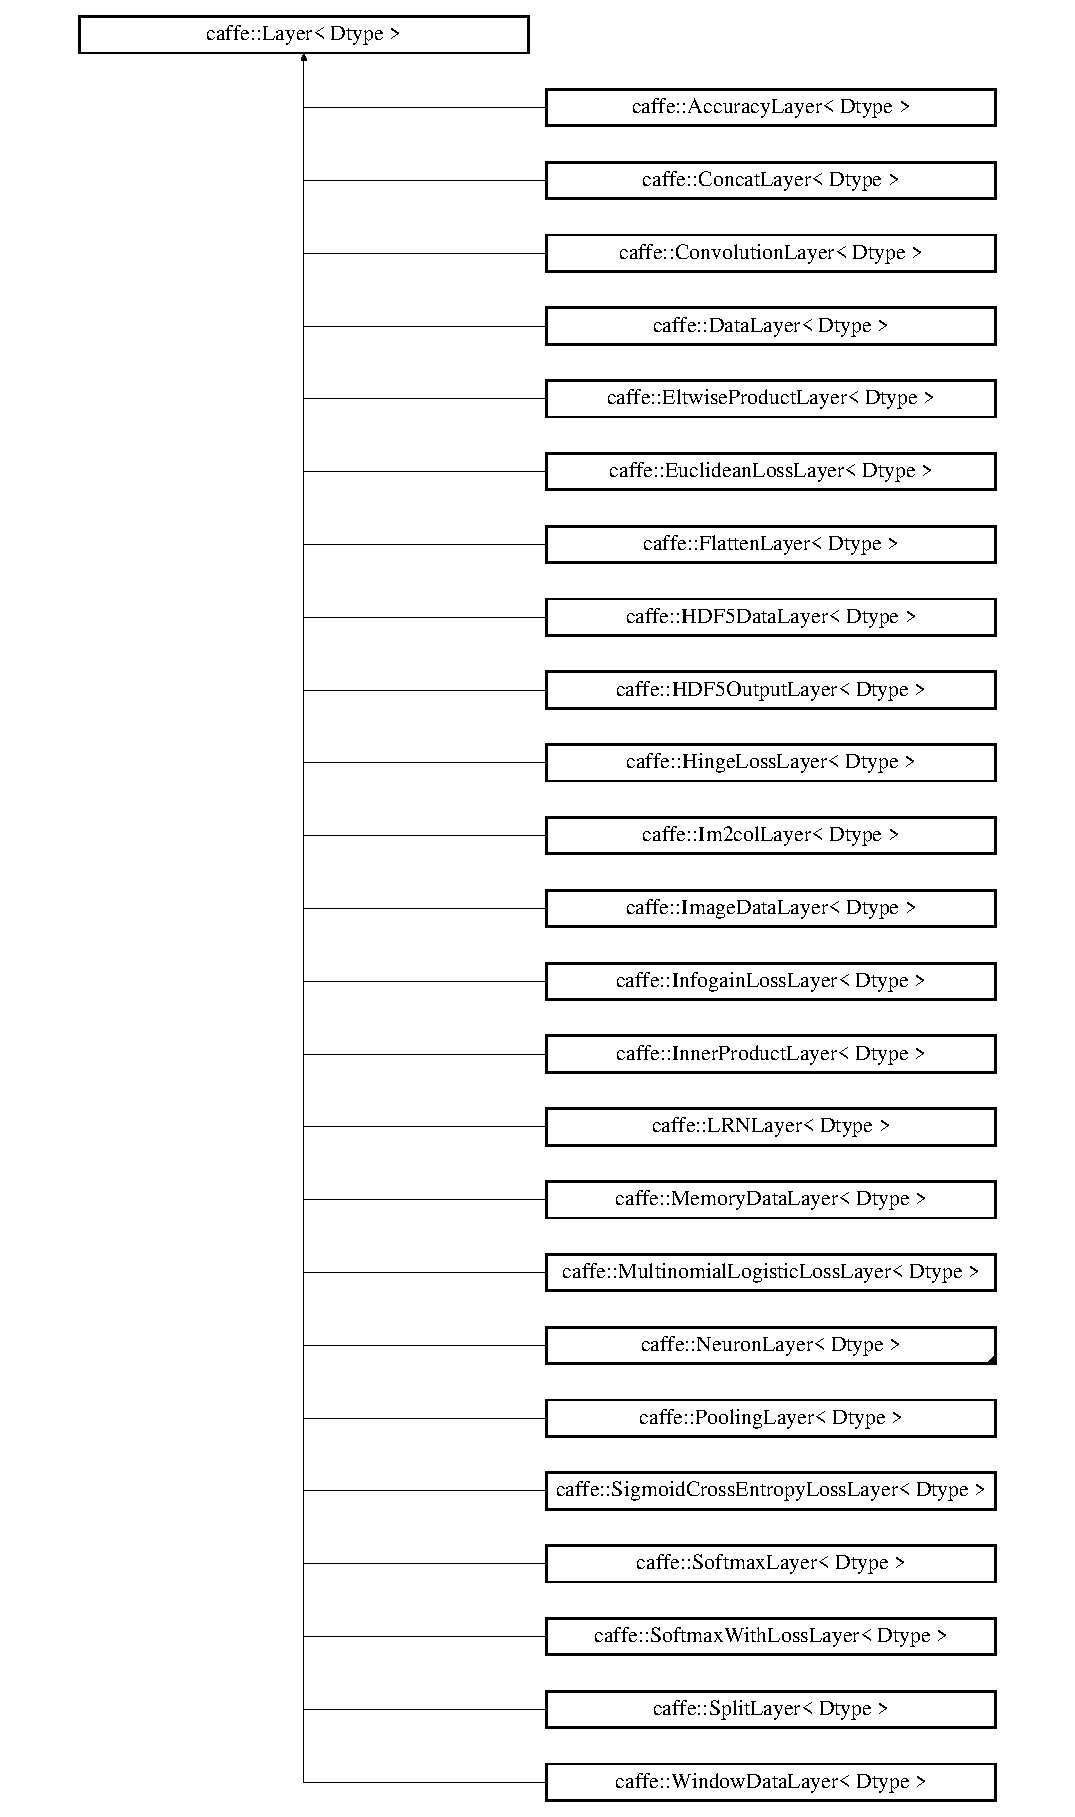
\includegraphics[height=12.000000cm]{classcaffe_1_1_layer}
\end{center}
\end{figure}
\subsection*{Public Member Functions}
\begin{DoxyCompactItemize}
\item 
\hyperlink{classcaffe_1_1_layer_a7b4e4ccea08c7b8b15acc6829d5735f6}{Layer} (const Layer\+Parameter \&param)
\item 
virtual \hyperlink{classcaffe_1_1_layer_aa9db88a6b9bdad8fceb1f79ea1cc2ef4}{$\sim$\+Layer} ()
\item 
virtual void \hyperlink{classcaffe_1_1_layer_abd13c6489c13953b4fbcfcf6880835d0}{Set\+Up} (const vector$<$ \hyperlink{classcaffe_1_1_blob}{Blob}$<$ Dtype $>$ $\ast$ $>$ \&bottom, vector$<$ \hyperlink{classcaffe_1_1_blob}{Blob}$<$ Dtype $>$ $\ast$ $>$ $\ast$top)=0
\item 
Dtype \hyperlink{classcaffe_1_1_layer_a31d00947960a1334be6e45c9a43d8d58}{Forward} (const vector$<$ \hyperlink{classcaffe_1_1_blob}{Blob}$<$ Dtype $>$ $\ast$ $>$ \&bottom, vector$<$ \hyperlink{classcaffe_1_1_blob}{Blob}$<$ Dtype $>$ $\ast$ $>$ $\ast$top)
\item 
void \hyperlink{classcaffe_1_1_layer_a4bcd2013ef9822dd21d122c97a87da83}{Backward} (const vector$<$ \hyperlink{classcaffe_1_1_blob}{Blob}$<$ Dtype $>$ $\ast$ $>$ \&top, const bool propagate\+\_\+down, vector$<$ \hyperlink{classcaffe_1_1_blob}{Blob}$<$ Dtype $>$ $\ast$ $>$ $\ast$bottom)
\item 
vector$<$ shared\+\_\+ptr$<$ \hyperlink{classcaffe_1_1_blob}{Blob}\\*
$<$ Dtype $>$ $>$ $>$ \& \hyperlink{classcaffe_1_1_layer_aaf4524ce8641a30a8a4784aee1b2b4c8}{blobs} ()
\item 
const Layer\+Parameter \& \hyperlink{classcaffe_1_1_layer_a6478a1086c96f32d928bc40f336cbb81}{layer\+\_\+param} ()
\item 
virtual void \hyperlink{classcaffe_1_1_layer_a4a1754828dda22cc8daa2f63377f3579}{To\+Proto} (Layer\+Parameter $\ast$param, bool write\+\_\+diff=false)
\end{DoxyCompactItemize}
\subsection*{Protected Member Functions}
\begin{DoxyCompactItemize}
\item 
virtual Dtype \hyperlink{classcaffe_1_1_layer_a8f7f61da3b8b3ca7f2394dee33873353}{Forward\+\_\+cpu} (const vector$<$ \hyperlink{classcaffe_1_1_blob}{Blob}$<$ Dtype $>$ $\ast$ $>$ \&bottom, vector$<$ \hyperlink{classcaffe_1_1_blob}{Blob}$<$ Dtype $>$ $\ast$ $>$ $\ast$top)=0
\item 
virtual Dtype \hyperlink{classcaffe_1_1_layer_a2d78dbf5d8bc36928bd8f6fcfbafbcef}{Forward\+\_\+gpu} (const vector$<$ \hyperlink{classcaffe_1_1_blob}{Blob}$<$ Dtype $>$ $\ast$ $>$ \&bottom, vector$<$ \hyperlink{classcaffe_1_1_blob}{Blob}$<$ Dtype $>$ $\ast$ $>$ $\ast$top)
\item 
virtual void \hyperlink{classcaffe_1_1_layer_ac2d82011d076237c67997f63e7ee4b80}{Backward\+\_\+cpu} (const vector$<$ \hyperlink{classcaffe_1_1_blob}{Blob}$<$ Dtype $>$ $\ast$ $>$ \&top, const bool propagate\+\_\+down, vector$<$ \hyperlink{classcaffe_1_1_blob}{Blob}$<$ Dtype $>$ $\ast$ $>$ $\ast$bottom)=0
\item 
virtual void \hyperlink{classcaffe_1_1_layer_adf07ffe1f22d2fd2b1b0ff475ef5a64b}{Backward\+\_\+gpu} (const vector$<$ \hyperlink{classcaffe_1_1_blob}{Blob}$<$ Dtype $>$ $\ast$ $>$ \&top, const bool propagate\+\_\+down, vector$<$ \hyperlink{classcaffe_1_1_blob}{Blob}$<$ Dtype $>$ $\ast$ $>$ $\ast$bottom)
\item 
\hyperlink{classcaffe_1_1_layer_a90730e177e4b3b3516b1b69ba2f6b06a}{D\+I\+S\+A\+B\+L\+E\+\_\+\+C\+O\+P\+Y\+\_\+\+A\+N\+D\+\_\+\+A\+S\+S\+I\+G\+N} (\hyperlink{classcaffe_1_1_layer}{Layer})
\end{DoxyCompactItemize}
\subsection*{Protected Attributes}
\begin{DoxyCompactItemize}
\item 
Layer\+Parameter \hyperlink{classcaffe_1_1_layer_a7ed12bb2df25c887e41d7ea9557fc701}{layer\+\_\+param\+\_\+}
\item 
vector$<$ shared\+\_\+ptr$<$ \hyperlink{classcaffe_1_1_blob}{Blob}\\*
$<$ Dtype $>$ $>$ $>$ \hyperlink{classcaffe_1_1_layer_a8073fcf2c139b47eb99ce71b346b1321}{blobs\+\_\+}
\end{DoxyCompactItemize}


\subsection{Constructor \& Destructor Documentation}
\hypertarget{classcaffe_1_1_layer_a7b4e4ccea08c7b8b15acc6829d5735f6}{\index{caffe\+::\+Layer@{caffe\+::\+Layer}!Layer@{Layer}}
\index{Layer@{Layer}!caffe\+::\+Layer@{caffe\+::\+Layer}}
\subsubsection[{Layer}]{\setlength{\rightskip}{0pt plus 5cm}template$<$typename Dtype$>$ {\bf caffe\+::\+Layer}$<$ Dtype $>$\+::{\bf Layer} (
\begin{DoxyParamCaption}
\item[{const Layer\+Parameter \&}]{param}
\end{DoxyParamCaption}
)\hspace{0.3cm}{\ttfamily [inline]}, {\ttfamily [explicit]}}}\label{classcaffe_1_1_layer_a7b4e4ccea08c7b8b15acc6829d5735f6}
\hypertarget{classcaffe_1_1_layer_aa9db88a6b9bdad8fceb1f79ea1cc2ef4}{\index{caffe\+::\+Layer@{caffe\+::\+Layer}!````~Layer@{$\sim$\+Layer}}
\index{````~Layer@{$\sim$\+Layer}!caffe\+::\+Layer@{caffe\+::\+Layer}}
\subsubsection[{$\sim$\+Layer}]{\setlength{\rightskip}{0pt plus 5cm}template$<$typename Dtype$>$ virtual {\bf caffe\+::\+Layer}$<$ Dtype $>$\+::$\sim${\bf Layer} (
\begin{DoxyParamCaption}
{}
\end{DoxyParamCaption}
)\hspace{0.3cm}{\ttfamily [inline]}, {\ttfamily [virtual]}}}\label{classcaffe_1_1_layer_aa9db88a6b9bdad8fceb1f79ea1cc2ef4}


\subsection{Member Function Documentation}
\hypertarget{classcaffe_1_1_layer_a4bcd2013ef9822dd21d122c97a87da83}{\index{caffe\+::\+Layer@{caffe\+::\+Layer}!Backward@{Backward}}
\index{Backward@{Backward}!caffe\+::\+Layer@{caffe\+::\+Layer}}
\subsubsection[{Backward}]{\setlength{\rightskip}{0pt plus 5cm}template$<$typename Dtype $>$ void {\bf caffe\+::\+Layer}$<$ Dtype $>$\+::Backward (
\begin{DoxyParamCaption}
\item[{const vector$<$ {\bf Blob}$<$ Dtype $>$ $\ast$ $>$ \&}]{top, }
\item[{const bool}]{propagate\+\_\+down, }
\item[{vector$<$ {\bf Blob}$<$ Dtype $>$ $\ast$ $>$ $\ast$}]{bottom}
\end{DoxyParamCaption}
)\hspace{0.3cm}{\ttfamily [inline]}}}\label{classcaffe_1_1_layer_a4bcd2013ef9822dd21d122c97a87da83}
\hypertarget{classcaffe_1_1_layer_ac2d82011d076237c67997f63e7ee4b80}{\index{caffe\+::\+Layer@{caffe\+::\+Layer}!Backward\+\_\+cpu@{Backward\+\_\+cpu}}
\index{Backward\+\_\+cpu@{Backward\+\_\+cpu}!caffe\+::\+Layer@{caffe\+::\+Layer}}
\subsubsection[{Backward\+\_\+cpu}]{\setlength{\rightskip}{0pt plus 5cm}template$<$typename Dtype$>$ virtual void {\bf caffe\+::\+Layer}$<$ Dtype $>$\+::Backward\+\_\+cpu (
\begin{DoxyParamCaption}
\item[{const vector$<$ {\bf Blob}$<$ Dtype $>$ $\ast$ $>$ \&}]{top, }
\item[{const bool}]{propagate\+\_\+down, }
\item[{vector$<$ {\bf Blob}$<$ Dtype $>$ $\ast$ $>$ $\ast$}]{bottom}
\end{DoxyParamCaption}
)\hspace{0.3cm}{\ttfamily [protected]}, {\ttfamily [pure virtual]}}}\label{classcaffe_1_1_layer_ac2d82011d076237c67997f63e7ee4b80}


Implemented in \hyperlink{classcaffe_1_1_window_data_layer_a39778e64942e652e2f9d8b41af621251}{caffe\+::\+Window\+Data\+Layer$<$ Dtype $>$}, \hyperlink{classcaffe_1_1_split_layer_ae9ef9d789fe7225af123010400b44100}{caffe\+::\+Split\+Layer$<$ Dtype $>$}, \hyperlink{classcaffe_1_1_softmax_with_loss_layer_ae969bcf16c6d99070e18d669053f8587}{caffe\+::\+Softmax\+With\+Loss\+Layer$<$ Dtype $>$}, \hyperlink{classcaffe_1_1_softmax_layer_a2f318816073f4585d6b84168fd2ce418}{caffe\+::\+Softmax\+Layer$<$ Dtype $>$}, \hyperlink{classcaffe_1_1_pooling_layer_aad07e6ab8b23155a971e2e78e87f0763}{caffe\+::\+Pooling\+Layer$<$ Dtype $>$}, \hyperlink{classcaffe_1_1_multinomial_logistic_loss_layer_a130cef8084d30fc789c401ec0310d587}{caffe\+::\+Multinomial\+Logistic\+Loss\+Layer$<$ Dtype $>$}, \hyperlink{classcaffe_1_1_memory_data_layer_ac85916554558f0ca7881bd3ee608865c}{caffe\+::\+Memory\+Data\+Layer$<$ Dtype $>$}, \hyperlink{classcaffe_1_1_l_r_n_layer_a67a331a12eece60b04ff2960164b78fe}{caffe\+::\+L\+R\+N\+Layer$<$ Dtype $>$}, \hyperlink{classcaffe_1_1_inner_product_layer_ab4f9892f3be7aef5d98777bca2dd8598}{caffe\+::\+Inner\+Product\+Layer$<$ Dtype $>$}, \hyperlink{classcaffe_1_1_infogain_loss_layer_a3fea9231eb9c3f1cd2f3989c54e475a8}{caffe\+::\+Infogain\+Loss\+Layer$<$ Dtype $>$}, \hyperlink{classcaffe_1_1_image_data_layer_aa94c13be8dcceb317b637c6ddf6cb0af}{caffe\+::\+Image\+Data\+Layer$<$ Dtype $>$}, \hyperlink{classcaffe_1_1_im2col_layer_ae6436f4287c23e62965f7c8216669ef2}{caffe\+::\+Im2col\+Layer$<$ Dtype $>$}, \hyperlink{classcaffe_1_1_hinge_loss_layer_a467c0d92debbaddecf6b18d4bbc31526}{caffe\+::\+Hinge\+Loss\+Layer$<$ Dtype $>$}, \hyperlink{classcaffe_1_1_h_d_f5_data_layer_a2c44e32bcde368d4afbb2b9f68f4e3f8}{caffe\+::\+H\+D\+F5\+Data\+Layer$<$ Dtype $>$}, \hyperlink{classcaffe_1_1_h_d_f5_output_layer_a805cc611664761d199b5eb54ba20de0c}{caffe\+::\+H\+D\+F5\+Output\+Layer$<$ Dtype $>$}, \hyperlink{classcaffe_1_1_flatten_layer_a5b7439a850684ebd8901180853809a50}{caffe\+::\+Flatten\+Layer$<$ Dtype $>$}, \hyperlink{classcaffe_1_1_euclidean_loss_layer_aeca6594a25c462a4764f6c2e07224b2d}{caffe\+::\+Euclidean\+Loss\+Layer$<$ Dtype $>$}, \hyperlink{classcaffe_1_1_eltwise_product_layer_a5d03ef5628726c95e71d425137e60d5e}{caffe\+::\+Eltwise\+Product\+Layer$<$ Dtype $>$}, \hyperlink{classcaffe_1_1_data_layer_a4b58dd246c6d1d1c3950f8c344c8b5ac}{caffe\+::\+Data\+Layer$<$ Dtype $>$}, \hyperlink{classcaffe_1_1_convolution_layer_a977898d74cd37fa2557f74322d419575}{caffe\+::\+Convolution\+Layer$<$ Dtype $>$}, \hyperlink{classcaffe_1_1_concat_layer_ad9f664216981e5f2248cdf88b49c5015}{caffe\+::\+Concat\+Layer$<$ Dtype $>$}, \hyperlink{classcaffe_1_1_accuracy_layer_a18aff36af82433e25eca1e0de3276d7f}{caffe\+::\+Accuracy\+Layer$<$ Dtype $>$}, \hyperlink{classcaffe_1_1_tan_h_layer_a26fc7022a7f0c474b160db428bbdc4a3}{caffe\+::\+Tan\+H\+Layer$<$ Dtype $>$}, \hyperlink{classcaffe_1_1_sigmoid_cross_entropy_loss_layer_a336c6f8453f30a598c280cc0259a5a95}{caffe\+::\+Sigmoid\+Cross\+Entropy\+Loss\+Layer$<$ Dtype $>$}, \hyperlink{classcaffe_1_1_sigmoid_layer_a4d99e969155f06a298205c94b9701492}{caffe\+::\+Sigmoid\+Layer$<$ Dtype $>$}, \hyperlink{classcaffe_1_1_re_l_u_layer_ac00cb9a11b3a63939f3bf07f787c6357}{caffe\+::\+Re\+L\+U\+Layer$<$ Dtype $>$}, \hyperlink{classcaffe_1_1_power_layer_a44971f370af2adc06adf814d9465a371}{caffe\+::\+Power\+Layer$<$ Dtype $>$}, \hyperlink{classcaffe_1_1_dropout_layer_aca25a2d883356b1aa5a8c0fe852dc8a1}{caffe\+::\+Dropout\+Layer$<$ Dtype $>$}, and \hyperlink{classcaffe_1_1_b_n_l_l_layer_acf58b70a8e5fafc303844a822dcf0e3b}{caffe\+::\+B\+N\+L\+L\+Layer$<$ Dtype $>$}.

\hypertarget{classcaffe_1_1_layer_adf07ffe1f22d2fd2b1b0ff475ef5a64b}{\index{caffe\+::\+Layer@{caffe\+::\+Layer}!Backward\+\_\+gpu@{Backward\+\_\+gpu}}
\index{Backward\+\_\+gpu@{Backward\+\_\+gpu}!caffe\+::\+Layer@{caffe\+::\+Layer}}
\subsubsection[{Backward\+\_\+gpu}]{\setlength{\rightskip}{0pt plus 5cm}template$<$typename Dtype$>$ virtual void {\bf caffe\+::\+Layer}$<$ Dtype $>$\+::Backward\+\_\+gpu (
\begin{DoxyParamCaption}
\item[{const vector$<$ {\bf Blob}$<$ Dtype $>$ $\ast$ $>$ \&}]{top, }
\item[{const bool}]{propagate\+\_\+down, }
\item[{vector$<$ {\bf Blob}$<$ Dtype $>$ $\ast$ $>$ $\ast$}]{bottom}
\end{DoxyParamCaption}
)\hspace{0.3cm}{\ttfamily [inline]}, {\ttfamily [protected]}, {\ttfamily [virtual]}}}\label{classcaffe_1_1_layer_adf07ffe1f22d2fd2b1b0ff475ef5a64b}


Reimplemented in \hyperlink{classcaffe_1_1_window_data_layer_ac008d7905f98366ae679a0fd6626abdb}{caffe\+::\+Window\+Data\+Layer$<$ Dtype $>$}, \hyperlink{classcaffe_1_1_split_layer_a22b01622ac43b4a8a4dbbd893f25ae32}{caffe\+::\+Split\+Layer$<$ Dtype $>$}, \hyperlink{classcaffe_1_1_softmax_with_loss_layer_a5274ccce6a8850e7bb61ac64ade39c8a}{caffe\+::\+Softmax\+With\+Loss\+Layer$<$ Dtype $>$}, \hyperlink{classcaffe_1_1_softmax_layer_a46febb93e499d1fccd68f406a3dd4bcb}{caffe\+::\+Softmax\+Layer$<$ Dtype $>$}, \hyperlink{classcaffe_1_1_pooling_layer_a90db5feba107ee64fb1c3cfacc0b2f38}{caffe\+::\+Pooling\+Layer$<$ Dtype $>$}, \hyperlink{classcaffe_1_1_memory_data_layer_ab209891a982c0962c78c36dedf2916ed}{caffe\+::\+Memory\+Data\+Layer$<$ Dtype $>$}, \hyperlink{classcaffe_1_1_l_r_n_layer_a37759b344e93a5d7f61caed89c1c8993}{caffe\+::\+L\+R\+N\+Layer$<$ Dtype $>$}, \hyperlink{classcaffe_1_1_inner_product_layer_a67252d33aaf6efb6ef5ce2e450cc4ca8}{caffe\+::\+Inner\+Product\+Layer$<$ Dtype $>$}, \hyperlink{classcaffe_1_1_image_data_layer_af467793e1c2184cd5016186c54167a20}{caffe\+::\+Image\+Data\+Layer$<$ Dtype $>$}, \hyperlink{classcaffe_1_1_im2col_layer_abe4feb385c1226f2d69ec47142ce0b06}{caffe\+::\+Im2col\+Layer$<$ Dtype $>$}, \hyperlink{classcaffe_1_1_h_d_f5_data_layer_ac2528e6eea1bbcd1d6e3b0e35a7595b8}{caffe\+::\+H\+D\+F5\+Data\+Layer$<$ Dtype $>$}, \hyperlink{classcaffe_1_1_h_d_f5_output_layer_a2018b7ab2f08f004bf967b177e1bb724}{caffe\+::\+H\+D\+F5\+Output\+Layer$<$ Dtype $>$}, \hyperlink{classcaffe_1_1_flatten_layer_ae5f1044beb9b5c4d60ff8fd5487ad338}{caffe\+::\+Flatten\+Layer$<$ Dtype $>$}, \hyperlink{classcaffe_1_1_eltwise_product_layer_a9d5b22fd37b476dd5cab2499c9a69a87}{caffe\+::\+Eltwise\+Product\+Layer$<$ Dtype $>$}, \hyperlink{classcaffe_1_1_data_layer_a7d9d69b7d2fbb6635b677ade18d9d8be}{caffe\+::\+Data\+Layer$<$ Dtype $>$}, \hyperlink{classcaffe_1_1_convolution_layer_a451a90070f9600b3bc33e0a9f9356ab2}{caffe\+::\+Convolution\+Layer$<$ Dtype $>$}, \hyperlink{classcaffe_1_1_concat_layer_a86ff8e3cd7ae4f06b23751b60d43ba76}{caffe\+::\+Concat\+Layer$<$ Dtype $>$}, \hyperlink{classcaffe_1_1_tan_h_layer_ae87d8ab7d2580ac38c3e11d87fdad983}{caffe\+::\+Tan\+H\+Layer$<$ Dtype $>$}, \hyperlink{classcaffe_1_1_sigmoid_cross_entropy_loss_layer_a7065249b414fc6eac3dd19d7ba4100f6}{caffe\+::\+Sigmoid\+Cross\+Entropy\+Loss\+Layer$<$ Dtype $>$}, \hyperlink{classcaffe_1_1_sigmoid_layer_a322bf664195dc8cad77ce5c48293a3f7}{caffe\+::\+Sigmoid\+Layer$<$ Dtype $>$}, \hyperlink{classcaffe_1_1_re_l_u_layer_aa3e55cef6a34c973c8ecab251520f154}{caffe\+::\+Re\+L\+U\+Layer$<$ Dtype $>$}, \hyperlink{classcaffe_1_1_power_layer_a4f127b9f0a3977137f56e6e7a1184241}{caffe\+::\+Power\+Layer$<$ Dtype $>$}, \hyperlink{classcaffe_1_1_dropout_layer_aad9d0019a2760866e47f8dc61b2ff3d9}{caffe\+::\+Dropout\+Layer$<$ Dtype $>$}, and \hyperlink{classcaffe_1_1_b_n_l_l_layer_a9732b6f05aac77d59e9a906a300b7bfe}{caffe\+::\+B\+N\+L\+L\+Layer$<$ Dtype $>$}.

\hypertarget{classcaffe_1_1_layer_aaf4524ce8641a30a8a4784aee1b2b4c8}{\index{caffe\+::\+Layer@{caffe\+::\+Layer}!blobs@{blobs}}
\index{blobs@{blobs}!caffe\+::\+Layer@{caffe\+::\+Layer}}
\subsubsection[{blobs}]{\setlength{\rightskip}{0pt plus 5cm}template$<$typename Dtype$>$ vector$<$shared\+\_\+ptr$<${\bf Blob}$<$Dtype$>$ $>$ $>$\& {\bf caffe\+::\+Layer}$<$ Dtype $>$\+::blobs (
\begin{DoxyParamCaption}
{}
\end{DoxyParamCaption}
)\hspace{0.3cm}{\ttfamily [inline]}}}\label{classcaffe_1_1_layer_aaf4524ce8641a30a8a4784aee1b2b4c8}
\hypertarget{classcaffe_1_1_layer_a90730e177e4b3b3516b1b69ba2f6b06a}{\index{caffe\+::\+Layer@{caffe\+::\+Layer}!D\+I\+S\+A\+B\+L\+E\+\_\+\+C\+O\+P\+Y\+\_\+\+A\+N\+D\+\_\+\+A\+S\+S\+I\+G\+N@{D\+I\+S\+A\+B\+L\+E\+\_\+\+C\+O\+P\+Y\+\_\+\+A\+N\+D\+\_\+\+A\+S\+S\+I\+G\+N}}
\index{D\+I\+S\+A\+B\+L\+E\+\_\+\+C\+O\+P\+Y\+\_\+\+A\+N\+D\+\_\+\+A\+S\+S\+I\+G\+N@{D\+I\+S\+A\+B\+L\+E\+\_\+\+C\+O\+P\+Y\+\_\+\+A\+N\+D\+\_\+\+A\+S\+S\+I\+G\+N}!caffe\+::\+Layer@{caffe\+::\+Layer}}
\subsubsection[{D\+I\+S\+A\+B\+L\+E\+\_\+\+C\+O\+P\+Y\+\_\+\+A\+N\+D\+\_\+\+A\+S\+S\+I\+G\+N}]{\setlength{\rightskip}{0pt plus 5cm}template$<$typename Dtype$>$ {\bf caffe\+::\+Layer}$<$ Dtype $>$\+::D\+I\+S\+A\+B\+L\+E\+\_\+\+C\+O\+P\+Y\+\_\+\+A\+N\+D\+\_\+\+A\+S\+S\+I\+G\+N (
\begin{DoxyParamCaption}
\item[{{\bf Layer}$<$ Dtype $>$}]{}
\end{DoxyParamCaption}
)\hspace{0.3cm}{\ttfamily [protected]}}}\label{classcaffe_1_1_layer_a90730e177e4b3b3516b1b69ba2f6b06a}
\hypertarget{classcaffe_1_1_layer_a31d00947960a1334be6e45c9a43d8d58}{\index{caffe\+::\+Layer@{caffe\+::\+Layer}!Forward@{Forward}}
\index{Forward@{Forward}!caffe\+::\+Layer@{caffe\+::\+Layer}}
\subsubsection[{Forward}]{\setlength{\rightskip}{0pt plus 5cm}template$<$typename Dtype $>$ Dtype {\bf caffe\+::\+Layer}$<$ Dtype $>$\+::Forward (
\begin{DoxyParamCaption}
\item[{const vector$<$ {\bf Blob}$<$ Dtype $>$ $\ast$ $>$ \&}]{bottom, }
\item[{vector$<$ {\bf Blob}$<$ Dtype $>$ $\ast$ $>$ $\ast$}]{top}
\end{DoxyParamCaption}
)\hspace{0.3cm}{\ttfamily [inline]}}}\label{classcaffe_1_1_layer_a31d00947960a1334be6e45c9a43d8d58}
\hypertarget{classcaffe_1_1_layer_a8f7f61da3b8b3ca7f2394dee33873353}{\index{caffe\+::\+Layer@{caffe\+::\+Layer}!Forward\+\_\+cpu@{Forward\+\_\+cpu}}
\index{Forward\+\_\+cpu@{Forward\+\_\+cpu}!caffe\+::\+Layer@{caffe\+::\+Layer}}
\subsubsection[{Forward\+\_\+cpu}]{\setlength{\rightskip}{0pt plus 5cm}template$<$typename Dtype$>$ virtual Dtype {\bf caffe\+::\+Layer}$<$ Dtype $>$\+::Forward\+\_\+cpu (
\begin{DoxyParamCaption}
\item[{const vector$<$ {\bf Blob}$<$ Dtype $>$ $\ast$ $>$ \&}]{bottom, }
\item[{vector$<$ {\bf Blob}$<$ Dtype $>$ $\ast$ $>$ $\ast$}]{top}
\end{DoxyParamCaption}
)\hspace{0.3cm}{\ttfamily [protected]}, {\ttfamily [pure virtual]}}}\label{classcaffe_1_1_layer_a8f7f61da3b8b3ca7f2394dee33873353}


Implemented in \hyperlink{classcaffe_1_1_window_data_layer_a2a2d216fc883126708892da7f1496d33}{caffe\+::\+Window\+Data\+Layer$<$ Dtype $>$}, \hyperlink{classcaffe_1_1_split_layer_acf59ddcda276674b1b315cfc0c48c861}{caffe\+::\+Split\+Layer$<$ Dtype $>$}, \hyperlink{classcaffe_1_1_softmax_with_loss_layer_a898274f4130f8180dca39b573726f8f8}{caffe\+::\+Softmax\+With\+Loss\+Layer$<$ Dtype $>$}, \hyperlink{classcaffe_1_1_softmax_layer_a11afab015d5240699e45c44b5c4b64ff}{caffe\+::\+Softmax\+Layer$<$ Dtype $>$}, \hyperlink{classcaffe_1_1_pooling_layer_a94e0eecfd992d045bd0b8b0cee4523f0}{caffe\+::\+Pooling\+Layer$<$ Dtype $>$}, \hyperlink{classcaffe_1_1_multinomial_logistic_loss_layer_a5c506ead552d2764df152dd9c90b768b}{caffe\+::\+Multinomial\+Logistic\+Loss\+Layer$<$ Dtype $>$}, \hyperlink{classcaffe_1_1_memory_data_layer_a124ae7ed94f0cad8a7c64b3c4b79eb33}{caffe\+::\+Memory\+Data\+Layer$<$ Dtype $>$}, \hyperlink{classcaffe_1_1_l_r_n_layer_a825208caabbaa227d532a5c0d780e77c}{caffe\+::\+L\+R\+N\+Layer$<$ Dtype $>$}, \hyperlink{classcaffe_1_1_inner_product_layer_afa97ce030d4fec47cca1bd758bc446f3}{caffe\+::\+Inner\+Product\+Layer$<$ Dtype $>$}, \hyperlink{classcaffe_1_1_infogain_loss_layer_ab5a8e36c29baa36e34b81a06d04043b6}{caffe\+::\+Infogain\+Loss\+Layer$<$ Dtype $>$}, \hyperlink{classcaffe_1_1_image_data_layer_a3093be55fa03cc281778ba230a05456c}{caffe\+::\+Image\+Data\+Layer$<$ Dtype $>$}, \hyperlink{classcaffe_1_1_im2col_layer_a635af15bcfdf2ec96913d75de5763328}{caffe\+::\+Im2col\+Layer$<$ Dtype $>$}, \hyperlink{classcaffe_1_1_hinge_loss_layer_a1e6922952af5ac6989b080ef8cf0c89a}{caffe\+::\+Hinge\+Loss\+Layer$<$ Dtype $>$}, \hyperlink{classcaffe_1_1_h_d_f5_data_layer_afb70fc6efdfffa6ee155abe193b53e3d}{caffe\+::\+H\+D\+F5\+Data\+Layer$<$ Dtype $>$}, \hyperlink{classcaffe_1_1_h_d_f5_output_layer_a91f77d8f66e4de8280e681f9155b20fa}{caffe\+::\+H\+D\+F5\+Output\+Layer$<$ Dtype $>$}, \hyperlink{classcaffe_1_1_flatten_layer_a53caee1cc9658db97e9daefbcdffdc12}{caffe\+::\+Flatten\+Layer$<$ Dtype $>$}, \hyperlink{classcaffe_1_1_euclidean_loss_layer_ab3b17e7f7064f68b253df8d463f44dfc}{caffe\+::\+Euclidean\+Loss\+Layer$<$ Dtype $>$}, \hyperlink{classcaffe_1_1_eltwise_product_layer_a0c3daabf8f8075f4e94879218941a348}{caffe\+::\+Eltwise\+Product\+Layer$<$ Dtype $>$}, \hyperlink{classcaffe_1_1_data_layer_a35e60c6ea0e3b8b57671d42853e956c3}{caffe\+::\+Data\+Layer$<$ Dtype $>$}, \hyperlink{classcaffe_1_1_convolution_layer_a53eb4114d914f019bc873818d4f8e53b}{caffe\+::\+Convolution\+Layer$<$ Dtype $>$}, \hyperlink{classcaffe_1_1_concat_layer_a8d0ef15036059a8b5545c886360148ae}{caffe\+::\+Concat\+Layer$<$ Dtype $>$}, \hyperlink{classcaffe_1_1_accuracy_layer_a6b009239ed19e1568fda06654af26e39}{caffe\+::\+Accuracy\+Layer$<$ Dtype $>$}, \hyperlink{classcaffe_1_1_tan_h_layer_ae60a4fb43459c050d1e03fa301d5bcaa}{caffe\+::\+Tan\+H\+Layer$<$ Dtype $>$}, \hyperlink{classcaffe_1_1_sigmoid_cross_entropy_loss_layer_abfc9e224038c2052c3bbc4372914b3db}{caffe\+::\+Sigmoid\+Cross\+Entropy\+Loss\+Layer$<$ Dtype $>$}, \hyperlink{classcaffe_1_1_sigmoid_layer_a0adfa69975f516a39d6996dfdc946973}{caffe\+::\+Sigmoid\+Layer$<$ Dtype $>$}, \hyperlink{classcaffe_1_1_re_l_u_layer_a4a9975e1e49982136fc6e8e478c122dd}{caffe\+::\+Re\+L\+U\+Layer$<$ Dtype $>$}, \hyperlink{classcaffe_1_1_power_layer_a3efa0e32fd71a6562838359915e05a03}{caffe\+::\+Power\+Layer$<$ Dtype $>$}, \hyperlink{classcaffe_1_1_dropout_layer_a031995973fec83788c03723d9855ec3f}{caffe\+::\+Dropout\+Layer$<$ Dtype $>$}, and \hyperlink{classcaffe_1_1_b_n_l_l_layer_a1a0cb5dd56ad7d93f0d70e93f00263b9}{caffe\+::\+B\+N\+L\+L\+Layer$<$ Dtype $>$}.

\hypertarget{classcaffe_1_1_layer_a2d78dbf5d8bc36928bd8f6fcfbafbcef}{\index{caffe\+::\+Layer@{caffe\+::\+Layer}!Forward\+\_\+gpu@{Forward\+\_\+gpu}}
\index{Forward\+\_\+gpu@{Forward\+\_\+gpu}!caffe\+::\+Layer@{caffe\+::\+Layer}}
\subsubsection[{Forward\+\_\+gpu}]{\setlength{\rightskip}{0pt plus 5cm}template$<$typename Dtype$>$ virtual Dtype {\bf caffe\+::\+Layer}$<$ Dtype $>$\+::Forward\+\_\+gpu (
\begin{DoxyParamCaption}
\item[{const vector$<$ {\bf Blob}$<$ Dtype $>$ $\ast$ $>$ \&}]{bottom, }
\item[{vector$<$ {\bf Blob}$<$ Dtype $>$ $\ast$ $>$ $\ast$}]{top}
\end{DoxyParamCaption}
)\hspace{0.3cm}{\ttfamily [inline]}, {\ttfamily [protected]}, {\ttfamily [virtual]}}}\label{classcaffe_1_1_layer_a2d78dbf5d8bc36928bd8f6fcfbafbcef}


Reimplemented in \hyperlink{classcaffe_1_1_window_data_layer_a920786219c1bad25f41c39212e2d6fab}{caffe\+::\+Window\+Data\+Layer$<$ Dtype $>$}, \hyperlink{classcaffe_1_1_split_layer_a846e3484a6db332c52f38e70e673a5b8}{caffe\+::\+Split\+Layer$<$ Dtype $>$}, \hyperlink{classcaffe_1_1_softmax_with_loss_layer_a38d8051ca05ca2dbb1af137d6ce42a42}{caffe\+::\+Softmax\+With\+Loss\+Layer$<$ Dtype $>$}, \hyperlink{classcaffe_1_1_softmax_layer_a37ede6eb847d766731b833e2f8923219}{caffe\+::\+Softmax\+Layer$<$ Dtype $>$}, \hyperlink{classcaffe_1_1_pooling_layer_a6997ba2f8adca32e201b2e3aa5271791}{caffe\+::\+Pooling\+Layer$<$ Dtype $>$}, \hyperlink{classcaffe_1_1_l_r_n_layer_ae6bf5efc998c6cc22fdfd64bf2b245c4}{caffe\+::\+L\+R\+N\+Layer$<$ Dtype $>$}, \hyperlink{classcaffe_1_1_inner_product_layer_a309180d8bbea21a281de52f3465ea786}{caffe\+::\+Inner\+Product\+Layer$<$ Dtype $>$}, \hyperlink{classcaffe_1_1_image_data_layer_a3719ea4c463b83e57ae7249e5e371332}{caffe\+::\+Image\+Data\+Layer$<$ Dtype $>$}, \hyperlink{classcaffe_1_1_im2col_layer_af60c215a0953742dc1ca2163f55bd9a7}{caffe\+::\+Im2col\+Layer$<$ Dtype $>$}, \hyperlink{classcaffe_1_1_h_d_f5_data_layer_ab1413b32f9b5ad2182c7fd88b85240c3}{caffe\+::\+H\+D\+F5\+Data\+Layer$<$ Dtype $>$}, \hyperlink{classcaffe_1_1_h_d_f5_output_layer_a9f78145efc3bb9ecc7d6a78a3e9c3856}{caffe\+::\+H\+D\+F5\+Output\+Layer$<$ Dtype $>$}, \hyperlink{classcaffe_1_1_flatten_layer_a30c8f30255ed20ef7351673aacdbe680}{caffe\+::\+Flatten\+Layer$<$ Dtype $>$}, \hyperlink{classcaffe_1_1_eltwise_product_layer_a53cf4aaa04a908dc7ed5ceee48f6054d}{caffe\+::\+Eltwise\+Product\+Layer$<$ Dtype $>$}, \hyperlink{classcaffe_1_1_data_layer_ae94ad93e1ad35123624e0aba0a2f03c6}{caffe\+::\+Data\+Layer$<$ Dtype $>$}, \hyperlink{classcaffe_1_1_convolution_layer_a1feac725539612918553e6b7bf299b4b}{caffe\+::\+Convolution\+Layer$<$ Dtype $>$}, \hyperlink{classcaffe_1_1_concat_layer_a92913d7f28a319354470e56fd306b628}{caffe\+::\+Concat\+Layer$<$ Dtype $>$}, \hyperlink{classcaffe_1_1_tan_h_layer_a9ab83424b20d909a8786043cc8139a33}{caffe\+::\+Tan\+H\+Layer$<$ Dtype $>$}, \hyperlink{classcaffe_1_1_sigmoid_cross_entropy_loss_layer_a255cf432942a246a456bbc8e4d499436}{caffe\+::\+Sigmoid\+Cross\+Entropy\+Loss\+Layer$<$ Dtype $>$}, \hyperlink{classcaffe_1_1_sigmoid_layer_af13a499a9aabf1f615291f47ed1728ea}{caffe\+::\+Sigmoid\+Layer$<$ Dtype $>$}, \hyperlink{classcaffe_1_1_re_l_u_layer_a28eefafa10d35ebd85bc94fa6ceb9e10}{caffe\+::\+Re\+L\+U\+Layer$<$ Dtype $>$}, \hyperlink{classcaffe_1_1_power_layer_ad59217de2d3c6d0c363b89713155eae5}{caffe\+::\+Power\+Layer$<$ Dtype $>$}, \hyperlink{classcaffe_1_1_dropout_layer_a7f568b33a08534687ee840a89e004a35}{caffe\+::\+Dropout\+Layer$<$ Dtype $>$}, and \hyperlink{classcaffe_1_1_b_n_l_l_layer_a880ed4501379ea518a66bc7126b974bc}{caffe\+::\+B\+N\+L\+L\+Layer$<$ Dtype $>$}.

\hypertarget{classcaffe_1_1_layer_a6478a1086c96f32d928bc40f336cbb81}{\index{caffe\+::\+Layer@{caffe\+::\+Layer}!layer\+\_\+param@{layer\+\_\+param}}
\index{layer\+\_\+param@{layer\+\_\+param}!caffe\+::\+Layer@{caffe\+::\+Layer}}
\subsubsection[{layer\+\_\+param}]{\setlength{\rightskip}{0pt plus 5cm}template$<$typename Dtype$>$ const Layer\+Parameter\& {\bf caffe\+::\+Layer}$<$ Dtype $>$\+::layer\+\_\+param (
\begin{DoxyParamCaption}
{}
\end{DoxyParamCaption}
)\hspace{0.3cm}{\ttfamily [inline]}}}\label{classcaffe_1_1_layer_a6478a1086c96f32d928bc40f336cbb81}
\hypertarget{classcaffe_1_1_layer_abd13c6489c13953b4fbcfcf6880835d0}{\index{caffe\+::\+Layer@{caffe\+::\+Layer}!Set\+Up@{Set\+Up}}
\index{Set\+Up@{Set\+Up}!caffe\+::\+Layer@{caffe\+::\+Layer}}
\subsubsection[{Set\+Up}]{\setlength{\rightskip}{0pt plus 5cm}template$<$typename Dtype$>$ virtual void {\bf caffe\+::\+Layer}$<$ Dtype $>$\+::Set\+Up (
\begin{DoxyParamCaption}
\item[{const vector$<$ {\bf Blob}$<$ Dtype $>$ $\ast$ $>$ \&}]{bottom, }
\item[{vector$<$ {\bf Blob}$<$ Dtype $>$ $\ast$ $>$ $\ast$}]{top}
\end{DoxyParamCaption}
)\hspace{0.3cm}{\ttfamily [pure virtual]}}}\label{classcaffe_1_1_layer_abd13c6489c13953b4fbcfcf6880835d0}


Implemented in \hyperlink{classcaffe_1_1_window_data_layer_a9fe034abb37141b76180edd2002a095b}{caffe\+::\+Window\+Data\+Layer$<$ Dtype $>$}, \hyperlink{classcaffe_1_1_split_layer_ae906b539de55e5b996b471e3c3510501}{caffe\+::\+Split\+Layer$<$ Dtype $>$}, \hyperlink{classcaffe_1_1_softmax_with_loss_layer_a4e29194f599dc4f08b5aa48a4f9cf87e}{caffe\+::\+Softmax\+With\+Loss\+Layer$<$ Dtype $>$}, \hyperlink{classcaffe_1_1_softmax_layer_ac6d690c48e66fa79f42938349e99a2e2}{caffe\+::\+Softmax\+Layer$<$ Dtype $>$}, \hyperlink{classcaffe_1_1_pooling_layer_ac88da7bd4cb54fceb0a22a6efc61292e}{caffe\+::\+Pooling\+Layer$<$ Dtype $>$}, \hyperlink{classcaffe_1_1_multinomial_logistic_loss_layer_af706bf27c3170a243660e7fe46ad0686}{caffe\+::\+Multinomial\+Logistic\+Loss\+Layer$<$ Dtype $>$}, \hyperlink{classcaffe_1_1_memory_data_layer_a276f9246a9ff0e6f016dfb54f00da88d}{caffe\+::\+Memory\+Data\+Layer$<$ Dtype $>$}, \hyperlink{classcaffe_1_1_l_r_n_layer_a107b66d7985241c54d861cb9d940cfc1}{caffe\+::\+L\+R\+N\+Layer$<$ Dtype $>$}, \hyperlink{classcaffe_1_1_inner_product_layer_a3e95f827d46406c96575d8852b4d68fe}{caffe\+::\+Inner\+Product\+Layer$<$ Dtype $>$}, \hyperlink{classcaffe_1_1_infogain_loss_layer_a22a1826f68b20911bcd2941e2284fd9e}{caffe\+::\+Infogain\+Loss\+Layer$<$ Dtype $>$}, \hyperlink{classcaffe_1_1_image_data_layer_a02eedd60b16ef4f2285cd75110a27226}{caffe\+::\+Image\+Data\+Layer$<$ Dtype $>$}, \hyperlink{classcaffe_1_1_im2col_layer_a869008ef04af4d7aed3e412e449b1aeb}{caffe\+::\+Im2col\+Layer$<$ Dtype $>$}, \hyperlink{classcaffe_1_1_hinge_loss_layer_a6674ffab4fc6a97a1545801dad068d42}{caffe\+::\+Hinge\+Loss\+Layer$<$ Dtype $>$}, \hyperlink{classcaffe_1_1_h_d_f5_data_layer_a1b1786da3b00f367508d5f89d8d7dd59}{caffe\+::\+H\+D\+F5\+Data\+Layer$<$ Dtype $>$}, \hyperlink{classcaffe_1_1_h_d_f5_output_layer_ac30de09e62b1ad98c377f48a7c271ee7}{caffe\+::\+H\+D\+F5\+Output\+Layer$<$ Dtype $>$}, \hyperlink{classcaffe_1_1_flatten_layer_a49568781c51bfd9e762007910127254e}{caffe\+::\+Flatten\+Layer$<$ Dtype $>$}, \hyperlink{classcaffe_1_1_euclidean_loss_layer_a636a0ded0ca547c4af9b150953bce124}{caffe\+::\+Euclidean\+Loss\+Layer$<$ Dtype $>$}, \hyperlink{classcaffe_1_1_eltwise_product_layer_ab24fdd7f4a2b47c95fbe80ed1cd5ee08}{caffe\+::\+Eltwise\+Product\+Layer$<$ Dtype $>$}, \hyperlink{classcaffe_1_1_data_layer_a157c4ee7c0a8c1b961a80c9a6432c7ea}{caffe\+::\+Data\+Layer$<$ Dtype $>$}, \hyperlink{classcaffe_1_1_convolution_layer_ad3eebbeb87db98a784aea2ddd8e8199d}{caffe\+::\+Convolution\+Layer$<$ Dtype $>$}, \hyperlink{classcaffe_1_1_concat_layer_ad479a513d943035c1415309ed61e62d8}{caffe\+::\+Concat\+Layer$<$ Dtype $>$}, \hyperlink{classcaffe_1_1_accuracy_layer_a5c18f1e710a9d59c0180ad2cd6dc4537}{caffe\+::\+Accuracy\+Layer$<$ Dtype $>$}, \hyperlink{classcaffe_1_1_sigmoid_cross_entropy_loss_layer_ab45ec795cdd1c1a31c767aeaf2ed2b91}{caffe\+::\+Sigmoid\+Cross\+Entropy\+Loss\+Layer$<$ Dtype $>$}, \hyperlink{classcaffe_1_1_power_layer_a56719890adf4fbf31f1b63729a9a92f8}{caffe\+::\+Power\+Layer$<$ Dtype $>$}, \hyperlink{classcaffe_1_1_dropout_layer_a1314d858640aa6ef2453c7cb6209be4e}{caffe\+::\+Dropout\+Layer$<$ Dtype $>$}, and \hyperlink{classcaffe_1_1_neuron_layer_a8441089c3e6f2434a2683de22698352a}{caffe\+::\+Neuron\+Layer$<$ Dtype $>$}.

\hypertarget{classcaffe_1_1_layer_a4a1754828dda22cc8daa2f63377f3579}{\index{caffe\+::\+Layer@{caffe\+::\+Layer}!To\+Proto@{To\+Proto}}
\index{To\+Proto@{To\+Proto}!caffe\+::\+Layer@{caffe\+::\+Layer}}
\subsubsection[{To\+Proto}]{\setlength{\rightskip}{0pt plus 5cm}template$<$typename Dtype $>$ void {\bf caffe\+::\+Layer}$<$ Dtype $>$\+::To\+Proto (
\begin{DoxyParamCaption}
\item[{Layer\+Parameter $\ast$}]{param, }
\item[{bool}]{write\+\_\+diff = {\ttfamily false}}
\end{DoxyParamCaption}
)\hspace{0.3cm}{\ttfamily [virtual]}}}\label{classcaffe_1_1_layer_a4a1754828dda22cc8daa2f63377f3579}


\subsection{Member Data Documentation}
\hypertarget{classcaffe_1_1_layer_a8073fcf2c139b47eb99ce71b346b1321}{\index{caffe\+::\+Layer@{caffe\+::\+Layer}!blobs\+\_\+@{blobs\+\_\+}}
\index{blobs\+\_\+@{blobs\+\_\+}!caffe\+::\+Layer@{caffe\+::\+Layer}}
\subsubsection[{blobs\+\_\+}]{\setlength{\rightskip}{0pt plus 5cm}template$<$typename Dtype$>$ vector$<$shared\+\_\+ptr$<${\bf Blob}$<$Dtype$>$ $>$ $>$ {\bf caffe\+::\+Layer}$<$ Dtype $>$\+::blobs\+\_\+\hspace{0.3cm}{\ttfamily [protected]}}}\label{classcaffe_1_1_layer_a8073fcf2c139b47eb99ce71b346b1321}
\hypertarget{classcaffe_1_1_layer_a7ed12bb2df25c887e41d7ea9557fc701}{\index{caffe\+::\+Layer@{caffe\+::\+Layer}!layer\+\_\+param\+\_\+@{layer\+\_\+param\+\_\+}}
\index{layer\+\_\+param\+\_\+@{layer\+\_\+param\+\_\+}!caffe\+::\+Layer@{caffe\+::\+Layer}}
\subsubsection[{layer\+\_\+param\+\_\+}]{\setlength{\rightskip}{0pt plus 5cm}template$<$typename Dtype$>$ Layer\+Parameter {\bf caffe\+::\+Layer}$<$ Dtype $>$\+::layer\+\_\+param\+\_\+\hspace{0.3cm}{\ttfamily [protected]}}}\label{classcaffe_1_1_layer_a7ed12bb2df25c887e41d7ea9557fc701}


The documentation for this class was generated from the following file\+:\begin{DoxyCompactItemize}
\item 
include/caffe/\hyperlink{layer_8hpp}{layer.\+hpp}\end{DoxyCompactItemize}

\hypertarget{classcaffe_1_1_l_r_n_layer}{\section{caffe\+:\+:L\+R\+N\+Layer$<$ Dtype $>$ Class Template Reference}
\label{classcaffe_1_1_l_r_n_layer}\index{caffe\+::\+L\+R\+N\+Layer$<$ Dtype $>$@{caffe\+::\+L\+R\+N\+Layer$<$ Dtype $>$}}
}


{\ttfamily \#include $<$vision\+\_\+layers.\+hpp$>$}

Inheritance diagram for caffe\+:\+:L\+R\+N\+Layer$<$ Dtype $>$\+:\begin{figure}[H]
\begin{center}
\leavevmode
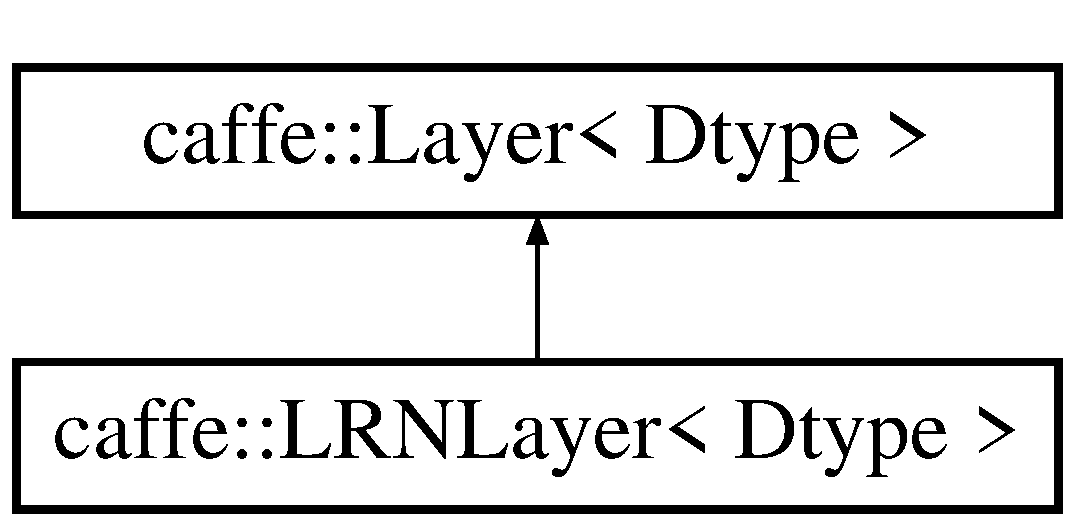
\includegraphics[height=2.000000cm]{classcaffe_1_1_l_r_n_layer}
\end{center}
\end{figure}
\subsection*{Public Member Functions}
\begin{DoxyCompactItemize}
\item 
\hyperlink{classcaffe_1_1_l_r_n_layer_a235b5f1b8fead8d1ddb9c29d627058fe}{L\+R\+N\+Layer} (const Layer\+Parameter \&param)
\item 
virtual void \hyperlink{classcaffe_1_1_l_r_n_layer_a107b66d7985241c54d861cb9d940cfc1}{Set\+Up} (const vector$<$ \hyperlink{classcaffe_1_1_blob}{Blob}$<$ Dtype $>$ $\ast$ $>$ \&bottom, vector$<$ \hyperlink{classcaffe_1_1_blob}{Blob}$<$ Dtype $>$ $\ast$ $>$ $\ast$top)
\end{DoxyCompactItemize}
\subsection*{Protected Member Functions}
\begin{DoxyCompactItemize}
\item 
virtual Dtype \hyperlink{classcaffe_1_1_l_r_n_layer_a825208caabbaa227d532a5c0d780e77c}{Forward\+\_\+cpu} (const vector$<$ \hyperlink{classcaffe_1_1_blob}{Blob}$<$ Dtype $>$ $\ast$ $>$ \&bottom, vector$<$ \hyperlink{classcaffe_1_1_blob}{Blob}$<$ Dtype $>$ $\ast$ $>$ $\ast$top)
\item 
virtual Dtype \hyperlink{classcaffe_1_1_l_r_n_layer_ae6bf5efc998c6cc22fdfd64bf2b245c4}{Forward\+\_\+gpu} (const vector$<$ \hyperlink{classcaffe_1_1_blob}{Blob}$<$ Dtype $>$ $\ast$ $>$ \&bottom, vector$<$ \hyperlink{classcaffe_1_1_blob}{Blob}$<$ Dtype $>$ $\ast$ $>$ $\ast$top)
\item 
virtual void \hyperlink{classcaffe_1_1_l_r_n_layer_a67a331a12eece60b04ff2960164b78fe}{Backward\+\_\+cpu} (const vector$<$ \hyperlink{classcaffe_1_1_blob}{Blob}$<$ Dtype $>$ $\ast$ $>$ \&top, const bool propagate\+\_\+down, vector$<$ \hyperlink{classcaffe_1_1_blob}{Blob}$<$ Dtype $>$ $\ast$ $>$ $\ast$bottom)
\item 
virtual void \hyperlink{classcaffe_1_1_l_r_n_layer_a37759b344e93a5d7f61caed89c1c8993}{Backward\+\_\+gpu} (const vector$<$ \hyperlink{classcaffe_1_1_blob}{Blob}$<$ Dtype $>$ $\ast$ $>$ \&top, const bool propagate\+\_\+down, vector$<$ \hyperlink{classcaffe_1_1_blob}{Blob}$<$ Dtype $>$ $\ast$ $>$ $\ast$bottom)
\item 
virtual Dtype \hyperlink{classcaffe_1_1_l_r_n_layer_aa4ede484dc14c32222fad968b7865522}{Cross\+Channel\+Forward\+\_\+cpu} (const vector$<$ \hyperlink{classcaffe_1_1_blob}{Blob}$<$ Dtype $>$ $\ast$ $>$ \&bottom, vector$<$ \hyperlink{classcaffe_1_1_blob}{Blob}$<$ Dtype $>$ $\ast$ $>$ $\ast$top)
\item 
virtual Dtype \hyperlink{classcaffe_1_1_l_r_n_layer_ad6cd5df675d0975034e58c9e09304e33}{Cross\+Channel\+Forward\+\_\+gpu} (const vector$<$ \hyperlink{classcaffe_1_1_blob}{Blob}$<$ Dtype $>$ $\ast$ $>$ \&bottom, vector$<$ \hyperlink{classcaffe_1_1_blob}{Blob}$<$ Dtype $>$ $\ast$ $>$ $\ast$top)
\item 
virtual Dtype \hyperlink{classcaffe_1_1_l_r_n_layer_a6f86e75a6b68f47e9e528644254057c2}{Within\+Channel\+Forward} (const vector$<$ \hyperlink{classcaffe_1_1_blob}{Blob}$<$ Dtype $>$ $\ast$ $>$ \&bottom, vector$<$ \hyperlink{classcaffe_1_1_blob}{Blob}$<$ Dtype $>$ $\ast$ $>$ $\ast$top)
\item 
virtual void \hyperlink{classcaffe_1_1_l_r_n_layer_ac2a6d21611db7683d6996988722d50a3}{Cross\+Channel\+Backward\+\_\+cpu} (const vector$<$ \hyperlink{classcaffe_1_1_blob}{Blob}$<$ Dtype $>$ $\ast$ $>$ \&top, const bool propagate\+\_\+down, vector$<$ \hyperlink{classcaffe_1_1_blob}{Blob}$<$ Dtype $>$ $\ast$ $>$ $\ast$bottom)
\item 
virtual void \hyperlink{classcaffe_1_1_l_r_n_layer_a5dc43ada322516ebd9cee01eb56e19f8}{Cross\+Channel\+Backward\+\_\+gpu} (const vector$<$ \hyperlink{classcaffe_1_1_blob}{Blob}$<$ Dtype $>$ $\ast$ $>$ \&top, const bool propagate\+\_\+down, vector$<$ \hyperlink{classcaffe_1_1_blob}{Blob}$<$ Dtype $>$ $\ast$ $>$ $\ast$bottom)
\item 
virtual void \hyperlink{classcaffe_1_1_l_r_n_layer_aef8f2723840441b902addf88aa309e07}{Within\+Channel\+Backward} (const vector$<$ \hyperlink{classcaffe_1_1_blob}{Blob}$<$ Dtype $>$ $\ast$ $>$ \&top, const bool propagate\+\_\+down, vector$<$ \hyperlink{classcaffe_1_1_blob}{Blob}$<$ Dtype $>$ $\ast$ $>$ $\ast$bottom)
\end{DoxyCompactItemize}
\subsection*{Protected Attributes}
\begin{DoxyCompactItemize}
\item 
int \hyperlink{classcaffe_1_1_l_r_n_layer_a4d74c3370e28abe013bf0fcc815fcc17}{size\+\_\+}
\item 
int \hyperlink{classcaffe_1_1_l_r_n_layer_a5d4a63f1279542a4fbe2780ba061f800}{pre\+\_\+pad\+\_\+}
\item 
Dtype \hyperlink{classcaffe_1_1_l_r_n_layer_ae5a9eaf89e4082afe166f0fa7ee3b4ed}{alpha\+\_\+}
\item 
Dtype \hyperlink{classcaffe_1_1_l_r_n_layer_aa0765abb189bb6be067494ea5cc925f2}{beta\+\_\+}
\item 
int \hyperlink{classcaffe_1_1_l_r_n_layer_ac68d88464a09f9deaf929908ffbaf345}{num\+\_\+}
\item 
int \hyperlink{classcaffe_1_1_l_r_n_layer_acd1bc62c5c9074c1df80f12d716f9a7a}{channels\+\_\+}
\item 
int \hyperlink{classcaffe_1_1_l_r_n_layer_a9fa09286b061a99713b4268259fdaad7}{height\+\_\+}
\item 
int \hyperlink{classcaffe_1_1_l_r_n_layer_a5b12d5c779f16e9b1caf4c3a6d581e09}{width\+\_\+}
\item 
\hyperlink{classcaffe_1_1_blob}{Blob}$<$ Dtype $>$ \hyperlink{classcaffe_1_1_l_r_n_layer_a61a44943c15c502c557df755d8ef4c6c}{scale\+\_\+}
\item 
shared\+\_\+ptr$<$ \hyperlink{classcaffe_1_1_split_layer}{Split\+Layer}$<$ Dtype $>$ $>$ \hyperlink{classcaffe_1_1_l_r_n_layer_a7126b6cbb83ddafb80c9d9dc6d44f88f}{split\+\_\+layer\+\_\+}
\item 
vector$<$ \hyperlink{classcaffe_1_1_blob}{Blob}$<$ Dtype $>$ $\ast$ $>$ \hyperlink{classcaffe_1_1_l_r_n_layer_a9b199156b8113800365c64c22e0e177a}{split\+\_\+top\+\_\+vec\+\_\+}
\item 
shared\+\_\+ptr$<$ \hyperlink{classcaffe_1_1_power_layer}{Power\+Layer}$<$ Dtype $>$ $>$ \hyperlink{classcaffe_1_1_l_r_n_layer_a440a40fc6ec9131fd8425dabe8a48fa9}{square\+\_\+layer\+\_\+}
\item 
\hyperlink{classcaffe_1_1_blob}{Blob}$<$ Dtype $>$ \hyperlink{classcaffe_1_1_l_r_n_layer_a750c4b6871af300f8de03b5eda197056}{square\+\_\+input\+\_\+}
\item 
\hyperlink{classcaffe_1_1_blob}{Blob}$<$ Dtype $>$ \hyperlink{classcaffe_1_1_l_r_n_layer_a50c1f72f225f69d344857fc55dc52ef9}{square\+\_\+output\+\_\+}
\item 
vector$<$ \hyperlink{classcaffe_1_1_blob}{Blob}$<$ Dtype $>$ $\ast$ $>$ \hyperlink{classcaffe_1_1_l_r_n_layer_a0361883b2eada25a56b5a90f5ff99cac}{square\+\_\+bottom\+\_\+vec\+\_\+}
\item 
vector$<$ \hyperlink{classcaffe_1_1_blob}{Blob}$<$ Dtype $>$ $\ast$ $>$ \hyperlink{classcaffe_1_1_l_r_n_layer_accfb1597e6045b09dcdb421ba7e92070}{square\+\_\+top\+\_\+vec\+\_\+}
\item 
shared\+\_\+ptr$<$ \hyperlink{classcaffe_1_1_pooling_layer}{Pooling\+Layer}$<$ Dtype $>$ $>$ \hyperlink{classcaffe_1_1_l_r_n_layer_a3d883b2d7022bd66e1ac2227400a1caa}{pool\+\_\+layer\+\_\+}
\item 
\hyperlink{classcaffe_1_1_blob}{Blob}$<$ Dtype $>$ \hyperlink{classcaffe_1_1_l_r_n_layer_a7dfcd31ed9694bdd48c9e80bdfe1e7a4}{pool\+\_\+output\+\_\+}
\item 
vector$<$ \hyperlink{classcaffe_1_1_blob}{Blob}$<$ Dtype $>$ $\ast$ $>$ \hyperlink{classcaffe_1_1_l_r_n_layer_af1d75143e7d103749575c3ee167e1c8d}{pool\+\_\+top\+\_\+vec\+\_\+}
\item 
shared\+\_\+ptr$<$ \hyperlink{classcaffe_1_1_power_layer}{Power\+Layer}$<$ Dtype $>$ $>$ \hyperlink{classcaffe_1_1_l_r_n_layer_a7d9446e995a4e4d1c27961159c1e7950}{power\+\_\+layer\+\_\+}
\item 
\hyperlink{classcaffe_1_1_blob}{Blob}$<$ Dtype $>$ \hyperlink{classcaffe_1_1_l_r_n_layer_adb51a5bb10b26a27835b2b19ecfe72b2}{power\+\_\+output\+\_\+}
\item 
vector$<$ \hyperlink{classcaffe_1_1_blob}{Blob}$<$ Dtype $>$ $\ast$ $>$ \hyperlink{classcaffe_1_1_l_r_n_layer_ac83227b50de568833235e7b2bdfbb8a8}{power\+\_\+top\+\_\+vec\+\_\+}
\item 
shared\+\_\+ptr\\*
$<$ \hyperlink{classcaffe_1_1_eltwise_product_layer}{Eltwise\+Product\+Layer}$<$ Dtype $>$ $>$ \hyperlink{classcaffe_1_1_l_r_n_layer_aa1b9baeea7f76ad06ec122ce279aeaeb}{product\+\_\+layer\+\_\+}
\item 
\hyperlink{classcaffe_1_1_blob}{Blob}$<$ Dtype $>$ \hyperlink{classcaffe_1_1_l_r_n_layer_ada65115660edfedc23fce996acc42c74}{product\+\_\+data\+\_\+input\+\_\+}
\item 
vector$<$ \hyperlink{classcaffe_1_1_blob}{Blob}$<$ Dtype $>$ $\ast$ $>$ \hyperlink{classcaffe_1_1_l_r_n_layer_ab1bf581b7cf42b36bdbad8333989a177}{product\+\_\+bottom\+\_\+vec\+\_\+}
\end{DoxyCompactItemize}


\subsection{Constructor \& Destructor Documentation}
\hypertarget{classcaffe_1_1_l_r_n_layer_a235b5f1b8fead8d1ddb9c29d627058fe}{\index{caffe\+::\+L\+R\+N\+Layer@{caffe\+::\+L\+R\+N\+Layer}!L\+R\+N\+Layer@{L\+R\+N\+Layer}}
\index{L\+R\+N\+Layer@{L\+R\+N\+Layer}!caffe\+::\+L\+R\+N\+Layer@{caffe\+::\+L\+R\+N\+Layer}}
\subsubsection[{L\+R\+N\+Layer}]{\setlength{\rightskip}{0pt plus 5cm}template$<$typename Dtype $>$ {\bf caffe\+::\+L\+R\+N\+Layer}$<$ Dtype $>$\+::{\bf L\+R\+N\+Layer} (
\begin{DoxyParamCaption}
\item[{const Layer\+Parameter \&}]{param}
\end{DoxyParamCaption}
)\hspace{0.3cm}{\ttfamily [inline]}, {\ttfamily [explicit]}}}\label{classcaffe_1_1_l_r_n_layer_a235b5f1b8fead8d1ddb9c29d627058fe}


\subsection{Member Function Documentation}
\hypertarget{classcaffe_1_1_l_r_n_layer_a67a331a12eece60b04ff2960164b78fe}{\index{caffe\+::\+L\+R\+N\+Layer@{caffe\+::\+L\+R\+N\+Layer}!Backward\+\_\+cpu@{Backward\+\_\+cpu}}
\index{Backward\+\_\+cpu@{Backward\+\_\+cpu}!caffe\+::\+L\+R\+N\+Layer@{caffe\+::\+L\+R\+N\+Layer}}
\subsubsection[{Backward\+\_\+cpu}]{\setlength{\rightskip}{0pt plus 5cm}template$<$typename Dtype $>$ void {\bf caffe\+::\+L\+R\+N\+Layer}$<$ Dtype $>$\+::Backward\+\_\+cpu (
\begin{DoxyParamCaption}
\item[{const vector$<$ {\bf Blob}$<$ Dtype $>$ $\ast$ $>$ \&}]{top, }
\item[{const bool}]{propagate\+\_\+down, }
\item[{vector$<$ {\bf Blob}$<$ Dtype $>$ $\ast$ $>$ $\ast$}]{bottom}
\end{DoxyParamCaption}
)\hspace{0.3cm}{\ttfamily [protected]}, {\ttfamily [virtual]}}}\label{classcaffe_1_1_l_r_n_layer_a67a331a12eece60b04ff2960164b78fe}


Implements \hyperlink{classcaffe_1_1_layer_ac2d82011d076237c67997f63e7ee4b80}{caffe\+::\+Layer$<$ Dtype $>$}.

\hypertarget{classcaffe_1_1_l_r_n_layer_a37759b344e93a5d7f61caed89c1c8993}{\index{caffe\+::\+L\+R\+N\+Layer@{caffe\+::\+L\+R\+N\+Layer}!Backward\+\_\+gpu@{Backward\+\_\+gpu}}
\index{Backward\+\_\+gpu@{Backward\+\_\+gpu}!caffe\+::\+L\+R\+N\+Layer@{caffe\+::\+L\+R\+N\+Layer}}
\subsubsection[{Backward\+\_\+gpu}]{\setlength{\rightskip}{0pt plus 5cm}template$<$typename Dtype $>$ void {\bf caffe\+::\+L\+R\+N\+Layer}$<$ Dtype $>$\+::Backward\+\_\+gpu (
\begin{DoxyParamCaption}
\item[{const vector$<$ {\bf Blob}$<$ Dtype $>$ $\ast$ $>$ \&}]{top, }
\item[{const bool}]{propagate\+\_\+down, }
\item[{vector$<$ {\bf Blob}$<$ Dtype $>$ $\ast$ $>$ $\ast$}]{bottom}
\end{DoxyParamCaption}
)\hspace{0.3cm}{\ttfamily [protected]}, {\ttfamily [virtual]}}}\label{classcaffe_1_1_l_r_n_layer_a37759b344e93a5d7f61caed89c1c8993}


Reimplemented from \hyperlink{classcaffe_1_1_layer_adf07ffe1f22d2fd2b1b0ff475ef5a64b}{caffe\+::\+Layer$<$ Dtype $>$}.

\hypertarget{classcaffe_1_1_l_r_n_layer_ac2a6d21611db7683d6996988722d50a3}{\index{caffe\+::\+L\+R\+N\+Layer@{caffe\+::\+L\+R\+N\+Layer}!Cross\+Channel\+Backward\+\_\+cpu@{Cross\+Channel\+Backward\+\_\+cpu}}
\index{Cross\+Channel\+Backward\+\_\+cpu@{Cross\+Channel\+Backward\+\_\+cpu}!caffe\+::\+L\+R\+N\+Layer@{caffe\+::\+L\+R\+N\+Layer}}
\subsubsection[{Cross\+Channel\+Backward\+\_\+cpu}]{\setlength{\rightskip}{0pt plus 5cm}template$<$typename Dtype $>$ void {\bf caffe\+::\+L\+R\+N\+Layer}$<$ Dtype $>$\+::Cross\+Channel\+Backward\+\_\+cpu (
\begin{DoxyParamCaption}
\item[{const vector$<$ {\bf Blob}$<$ Dtype $>$ $\ast$ $>$ \&}]{top, }
\item[{const bool}]{propagate\+\_\+down, }
\item[{vector$<$ {\bf Blob}$<$ Dtype $>$ $\ast$ $>$ $\ast$}]{bottom}
\end{DoxyParamCaption}
)\hspace{0.3cm}{\ttfamily [protected]}, {\ttfamily [virtual]}}}\label{classcaffe_1_1_l_r_n_layer_ac2a6d21611db7683d6996988722d50a3}
\hypertarget{classcaffe_1_1_l_r_n_layer_a5dc43ada322516ebd9cee01eb56e19f8}{\index{caffe\+::\+L\+R\+N\+Layer@{caffe\+::\+L\+R\+N\+Layer}!Cross\+Channel\+Backward\+\_\+gpu@{Cross\+Channel\+Backward\+\_\+gpu}}
\index{Cross\+Channel\+Backward\+\_\+gpu@{Cross\+Channel\+Backward\+\_\+gpu}!caffe\+::\+L\+R\+N\+Layer@{caffe\+::\+L\+R\+N\+Layer}}
\subsubsection[{Cross\+Channel\+Backward\+\_\+gpu}]{\setlength{\rightskip}{0pt plus 5cm}template$<$typename Dtype $>$ void {\bf caffe\+::\+L\+R\+N\+Layer}$<$ Dtype $>$\+::Cross\+Channel\+Backward\+\_\+gpu (
\begin{DoxyParamCaption}
\item[{const vector$<$ {\bf Blob}$<$ Dtype $>$ $\ast$ $>$ \&}]{top, }
\item[{const bool}]{propagate\+\_\+down, }
\item[{vector$<$ {\bf Blob}$<$ Dtype $>$ $\ast$ $>$ $\ast$}]{bottom}
\end{DoxyParamCaption}
)\hspace{0.3cm}{\ttfamily [protected]}, {\ttfamily [virtual]}}}\label{classcaffe_1_1_l_r_n_layer_a5dc43ada322516ebd9cee01eb56e19f8}
\hypertarget{classcaffe_1_1_l_r_n_layer_aa4ede484dc14c32222fad968b7865522}{\index{caffe\+::\+L\+R\+N\+Layer@{caffe\+::\+L\+R\+N\+Layer}!Cross\+Channel\+Forward\+\_\+cpu@{Cross\+Channel\+Forward\+\_\+cpu}}
\index{Cross\+Channel\+Forward\+\_\+cpu@{Cross\+Channel\+Forward\+\_\+cpu}!caffe\+::\+L\+R\+N\+Layer@{caffe\+::\+L\+R\+N\+Layer}}
\subsubsection[{Cross\+Channel\+Forward\+\_\+cpu}]{\setlength{\rightskip}{0pt plus 5cm}template$<$typename Dtype $>$ Dtype {\bf caffe\+::\+L\+R\+N\+Layer}$<$ Dtype $>$\+::Cross\+Channel\+Forward\+\_\+cpu (
\begin{DoxyParamCaption}
\item[{const vector$<$ {\bf Blob}$<$ Dtype $>$ $\ast$ $>$ \&}]{bottom, }
\item[{vector$<$ {\bf Blob}$<$ Dtype $>$ $\ast$ $>$ $\ast$}]{top}
\end{DoxyParamCaption}
)\hspace{0.3cm}{\ttfamily [protected]}, {\ttfamily [virtual]}}}\label{classcaffe_1_1_l_r_n_layer_aa4ede484dc14c32222fad968b7865522}
\hypertarget{classcaffe_1_1_l_r_n_layer_ad6cd5df675d0975034e58c9e09304e33}{\index{caffe\+::\+L\+R\+N\+Layer@{caffe\+::\+L\+R\+N\+Layer}!Cross\+Channel\+Forward\+\_\+gpu@{Cross\+Channel\+Forward\+\_\+gpu}}
\index{Cross\+Channel\+Forward\+\_\+gpu@{Cross\+Channel\+Forward\+\_\+gpu}!caffe\+::\+L\+R\+N\+Layer@{caffe\+::\+L\+R\+N\+Layer}}
\subsubsection[{Cross\+Channel\+Forward\+\_\+gpu}]{\setlength{\rightskip}{0pt plus 5cm}template$<$typename Dtype $>$ Dtype {\bf caffe\+::\+L\+R\+N\+Layer}$<$ Dtype $>$\+::Cross\+Channel\+Forward\+\_\+gpu (
\begin{DoxyParamCaption}
\item[{const vector$<$ {\bf Blob}$<$ Dtype $>$ $\ast$ $>$ \&}]{bottom, }
\item[{vector$<$ {\bf Blob}$<$ Dtype $>$ $\ast$ $>$ $\ast$}]{top}
\end{DoxyParamCaption}
)\hspace{0.3cm}{\ttfamily [protected]}, {\ttfamily [virtual]}}}\label{classcaffe_1_1_l_r_n_layer_ad6cd5df675d0975034e58c9e09304e33}
\hypertarget{classcaffe_1_1_l_r_n_layer_a825208caabbaa227d532a5c0d780e77c}{\index{caffe\+::\+L\+R\+N\+Layer@{caffe\+::\+L\+R\+N\+Layer}!Forward\+\_\+cpu@{Forward\+\_\+cpu}}
\index{Forward\+\_\+cpu@{Forward\+\_\+cpu}!caffe\+::\+L\+R\+N\+Layer@{caffe\+::\+L\+R\+N\+Layer}}
\subsubsection[{Forward\+\_\+cpu}]{\setlength{\rightskip}{0pt plus 5cm}template$<$typename Dtype $>$ Dtype {\bf caffe\+::\+L\+R\+N\+Layer}$<$ Dtype $>$\+::Forward\+\_\+cpu (
\begin{DoxyParamCaption}
\item[{const vector$<$ {\bf Blob}$<$ Dtype $>$ $\ast$ $>$ \&}]{bottom, }
\item[{vector$<$ {\bf Blob}$<$ Dtype $>$ $\ast$ $>$ $\ast$}]{top}
\end{DoxyParamCaption}
)\hspace{0.3cm}{\ttfamily [protected]}, {\ttfamily [virtual]}}}\label{classcaffe_1_1_l_r_n_layer_a825208caabbaa227d532a5c0d780e77c}


Implements \hyperlink{classcaffe_1_1_layer_a8f7f61da3b8b3ca7f2394dee33873353}{caffe\+::\+Layer$<$ Dtype $>$}.

\hypertarget{classcaffe_1_1_l_r_n_layer_ae6bf5efc998c6cc22fdfd64bf2b245c4}{\index{caffe\+::\+L\+R\+N\+Layer@{caffe\+::\+L\+R\+N\+Layer}!Forward\+\_\+gpu@{Forward\+\_\+gpu}}
\index{Forward\+\_\+gpu@{Forward\+\_\+gpu}!caffe\+::\+L\+R\+N\+Layer@{caffe\+::\+L\+R\+N\+Layer}}
\subsubsection[{Forward\+\_\+gpu}]{\setlength{\rightskip}{0pt plus 5cm}template$<$typename Dtype $>$ Dtype {\bf caffe\+::\+L\+R\+N\+Layer}$<$ Dtype $>$\+::Forward\+\_\+gpu (
\begin{DoxyParamCaption}
\item[{const vector$<$ {\bf Blob}$<$ Dtype $>$ $\ast$ $>$ \&}]{bottom, }
\item[{vector$<$ {\bf Blob}$<$ Dtype $>$ $\ast$ $>$ $\ast$}]{top}
\end{DoxyParamCaption}
)\hspace{0.3cm}{\ttfamily [protected]}, {\ttfamily [virtual]}}}\label{classcaffe_1_1_l_r_n_layer_ae6bf5efc998c6cc22fdfd64bf2b245c4}


Reimplemented from \hyperlink{classcaffe_1_1_layer_a2d78dbf5d8bc36928bd8f6fcfbafbcef}{caffe\+::\+Layer$<$ Dtype $>$}.

\hypertarget{classcaffe_1_1_l_r_n_layer_a107b66d7985241c54d861cb9d940cfc1}{\index{caffe\+::\+L\+R\+N\+Layer@{caffe\+::\+L\+R\+N\+Layer}!Set\+Up@{Set\+Up}}
\index{Set\+Up@{Set\+Up}!caffe\+::\+L\+R\+N\+Layer@{caffe\+::\+L\+R\+N\+Layer}}
\subsubsection[{Set\+Up}]{\setlength{\rightskip}{0pt plus 5cm}template$<$typename Dtype $>$ void {\bf caffe\+::\+L\+R\+N\+Layer}$<$ Dtype $>$\+::Set\+Up (
\begin{DoxyParamCaption}
\item[{const vector$<$ {\bf Blob}$<$ Dtype $>$ $\ast$ $>$ \&}]{bottom, }
\item[{vector$<$ {\bf Blob}$<$ Dtype $>$ $\ast$ $>$ $\ast$}]{top}
\end{DoxyParamCaption}
)\hspace{0.3cm}{\ttfamily [virtual]}}}\label{classcaffe_1_1_l_r_n_layer_a107b66d7985241c54d861cb9d940cfc1}


Implements \hyperlink{classcaffe_1_1_layer_abd13c6489c13953b4fbcfcf6880835d0}{caffe\+::\+Layer$<$ Dtype $>$}.

\hypertarget{classcaffe_1_1_l_r_n_layer_aef8f2723840441b902addf88aa309e07}{\index{caffe\+::\+L\+R\+N\+Layer@{caffe\+::\+L\+R\+N\+Layer}!Within\+Channel\+Backward@{Within\+Channel\+Backward}}
\index{Within\+Channel\+Backward@{Within\+Channel\+Backward}!caffe\+::\+L\+R\+N\+Layer@{caffe\+::\+L\+R\+N\+Layer}}
\subsubsection[{Within\+Channel\+Backward}]{\setlength{\rightskip}{0pt plus 5cm}template$<$typename Dtype $>$ void {\bf caffe\+::\+L\+R\+N\+Layer}$<$ Dtype $>$\+::Within\+Channel\+Backward (
\begin{DoxyParamCaption}
\item[{const vector$<$ {\bf Blob}$<$ Dtype $>$ $\ast$ $>$ \&}]{top, }
\item[{const bool}]{propagate\+\_\+down, }
\item[{vector$<$ {\bf Blob}$<$ Dtype $>$ $\ast$ $>$ $\ast$}]{bottom}
\end{DoxyParamCaption}
)\hspace{0.3cm}{\ttfamily [protected]}, {\ttfamily [virtual]}}}\label{classcaffe_1_1_l_r_n_layer_aef8f2723840441b902addf88aa309e07}
\hypertarget{classcaffe_1_1_l_r_n_layer_a6f86e75a6b68f47e9e528644254057c2}{\index{caffe\+::\+L\+R\+N\+Layer@{caffe\+::\+L\+R\+N\+Layer}!Within\+Channel\+Forward@{Within\+Channel\+Forward}}
\index{Within\+Channel\+Forward@{Within\+Channel\+Forward}!caffe\+::\+L\+R\+N\+Layer@{caffe\+::\+L\+R\+N\+Layer}}
\subsubsection[{Within\+Channel\+Forward}]{\setlength{\rightskip}{0pt plus 5cm}template$<$typename Dtype $>$ Dtype {\bf caffe\+::\+L\+R\+N\+Layer}$<$ Dtype $>$\+::Within\+Channel\+Forward (
\begin{DoxyParamCaption}
\item[{const vector$<$ {\bf Blob}$<$ Dtype $>$ $\ast$ $>$ \&}]{bottom, }
\item[{vector$<$ {\bf Blob}$<$ Dtype $>$ $\ast$ $>$ $\ast$}]{top}
\end{DoxyParamCaption}
)\hspace{0.3cm}{\ttfamily [protected]}, {\ttfamily [virtual]}}}\label{classcaffe_1_1_l_r_n_layer_a6f86e75a6b68f47e9e528644254057c2}


\subsection{Member Data Documentation}
\hypertarget{classcaffe_1_1_l_r_n_layer_ae5a9eaf89e4082afe166f0fa7ee3b4ed}{\index{caffe\+::\+L\+R\+N\+Layer@{caffe\+::\+L\+R\+N\+Layer}!alpha\+\_\+@{alpha\+\_\+}}
\index{alpha\+\_\+@{alpha\+\_\+}!caffe\+::\+L\+R\+N\+Layer@{caffe\+::\+L\+R\+N\+Layer}}
\subsubsection[{alpha\+\_\+}]{\setlength{\rightskip}{0pt plus 5cm}template$<$typename Dtype $>$ Dtype {\bf caffe\+::\+L\+R\+N\+Layer}$<$ Dtype $>$\+::alpha\+\_\+\hspace{0.3cm}{\ttfamily [protected]}}}\label{classcaffe_1_1_l_r_n_layer_ae5a9eaf89e4082afe166f0fa7ee3b4ed}
\hypertarget{classcaffe_1_1_l_r_n_layer_aa0765abb189bb6be067494ea5cc925f2}{\index{caffe\+::\+L\+R\+N\+Layer@{caffe\+::\+L\+R\+N\+Layer}!beta\+\_\+@{beta\+\_\+}}
\index{beta\+\_\+@{beta\+\_\+}!caffe\+::\+L\+R\+N\+Layer@{caffe\+::\+L\+R\+N\+Layer}}
\subsubsection[{beta\+\_\+}]{\setlength{\rightskip}{0pt plus 5cm}template$<$typename Dtype $>$ Dtype {\bf caffe\+::\+L\+R\+N\+Layer}$<$ Dtype $>$\+::beta\+\_\+\hspace{0.3cm}{\ttfamily [protected]}}}\label{classcaffe_1_1_l_r_n_layer_aa0765abb189bb6be067494ea5cc925f2}
\hypertarget{classcaffe_1_1_l_r_n_layer_acd1bc62c5c9074c1df80f12d716f9a7a}{\index{caffe\+::\+L\+R\+N\+Layer@{caffe\+::\+L\+R\+N\+Layer}!channels\+\_\+@{channels\+\_\+}}
\index{channels\+\_\+@{channels\+\_\+}!caffe\+::\+L\+R\+N\+Layer@{caffe\+::\+L\+R\+N\+Layer}}
\subsubsection[{channels\+\_\+}]{\setlength{\rightskip}{0pt plus 5cm}template$<$typename Dtype $>$ int {\bf caffe\+::\+L\+R\+N\+Layer}$<$ Dtype $>$\+::channels\+\_\+\hspace{0.3cm}{\ttfamily [protected]}}}\label{classcaffe_1_1_l_r_n_layer_acd1bc62c5c9074c1df80f12d716f9a7a}
\hypertarget{classcaffe_1_1_l_r_n_layer_a9fa09286b061a99713b4268259fdaad7}{\index{caffe\+::\+L\+R\+N\+Layer@{caffe\+::\+L\+R\+N\+Layer}!height\+\_\+@{height\+\_\+}}
\index{height\+\_\+@{height\+\_\+}!caffe\+::\+L\+R\+N\+Layer@{caffe\+::\+L\+R\+N\+Layer}}
\subsubsection[{height\+\_\+}]{\setlength{\rightskip}{0pt plus 5cm}template$<$typename Dtype $>$ int {\bf caffe\+::\+L\+R\+N\+Layer}$<$ Dtype $>$\+::height\+\_\+\hspace{0.3cm}{\ttfamily [protected]}}}\label{classcaffe_1_1_l_r_n_layer_a9fa09286b061a99713b4268259fdaad7}
\hypertarget{classcaffe_1_1_l_r_n_layer_ac68d88464a09f9deaf929908ffbaf345}{\index{caffe\+::\+L\+R\+N\+Layer@{caffe\+::\+L\+R\+N\+Layer}!num\+\_\+@{num\+\_\+}}
\index{num\+\_\+@{num\+\_\+}!caffe\+::\+L\+R\+N\+Layer@{caffe\+::\+L\+R\+N\+Layer}}
\subsubsection[{num\+\_\+}]{\setlength{\rightskip}{0pt plus 5cm}template$<$typename Dtype $>$ int {\bf caffe\+::\+L\+R\+N\+Layer}$<$ Dtype $>$\+::num\+\_\+\hspace{0.3cm}{\ttfamily [protected]}}}\label{classcaffe_1_1_l_r_n_layer_ac68d88464a09f9deaf929908ffbaf345}
\hypertarget{classcaffe_1_1_l_r_n_layer_a3d883b2d7022bd66e1ac2227400a1caa}{\index{caffe\+::\+L\+R\+N\+Layer@{caffe\+::\+L\+R\+N\+Layer}!pool\+\_\+layer\+\_\+@{pool\+\_\+layer\+\_\+}}
\index{pool\+\_\+layer\+\_\+@{pool\+\_\+layer\+\_\+}!caffe\+::\+L\+R\+N\+Layer@{caffe\+::\+L\+R\+N\+Layer}}
\subsubsection[{pool\+\_\+layer\+\_\+}]{\setlength{\rightskip}{0pt plus 5cm}template$<$typename Dtype $>$ shared\+\_\+ptr$<${\bf Pooling\+Layer}$<$Dtype$>$ $>$ {\bf caffe\+::\+L\+R\+N\+Layer}$<$ Dtype $>$\+::pool\+\_\+layer\+\_\+\hspace{0.3cm}{\ttfamily [protected]}}}\label{classcaffe_1_1_l_r_n_layer_a3d883b2d7022bd66e1ac2227400a1caa}
\hypertarget{classcaffe_1_1_l_r_n_layer_a7dfcd31ed9694bdd48c9e80bdfe1e7a4}{\index{caffe\+::\+L\+R\+N\+Layer@{caffe\+::\+L\+R\+N\+Layer}!pool\+\_\+output\+\_\+@{pool\+\_\+output\+\_\+}}
\index{pool\+\_\+output\+\_\+@{pool\+\_\+output\+\_\+}!caffe\+::\+L\+R\+N\+Layer@{caffe\+::\+L\+R\+N\+Layer}}
\subsubsection[{pool\+\_\+output\+\_\+}]{\setlength{\rightskip}{0pt plus 5cm}template$<$typename Dtype $>$ {\bf Blob}$<$Dtype$>$ {\bf caffe\+::\+L\+R\+N\+Layer}$<$ Dtype $>$\+::pool\+\_\+output\+\_\+\hspace{0.3cm}{\ttfamily [protected]}}}\label{classcaffe_1_1_l_r_n_layer_a7dfcd31ed9694bdd48c9e80bdfe1e7a4}
\hypertarget{classcaffe_1_1_l_r_n_layer_af1d75143e7d103749575c3ee167e1c8d}{\index{caffe\+::\+L\+R\+N\+Layer@{caffe\+::\+L\+R\+N\+Layer}!pool\+\_\+top\+\_\+vec\+\_\+@{pool\+\_\+top\+\_\+vec\+\_\+}}
\index{pool\+\_\+top\+\_\+vec\+\_\+@{pool\+\_\+top\+\_\+vec\+\_\+}!caffe\+::\+L\+R\+N\+Layer@{caffe\+::\+L\+R\+N\+Layer}}
\subsubsection[{pool\+\_\+top\+\_\+vec\+\_\+}]{\setlength{\rightskip}{0pt plus 5cm}template$<$typename Dtype $>$ vector$<${\bf Blob}$<$Dtype$>$$\ast$$>$ {\bf caffe\+::\+L\+R\+N\+Layer}$<$ Dtype $>$\+::pool\+\_\+top\+\_\+vec\+\_\+\hspace{0.3cm}{\ttfamily [protected]}}}\label{classcaffe_1_1_l_r_n_layer_af1d75143e7d103749575c3ee167e1c8d}
\hypertarget{classcaffe_1_1_l_r_n_layer_a7d9446e995a4e4d1c27961159c1e7950}{\index{caffe\+::\+L\+R\+N\+Layer@{caffe\+::\+L\+R\+N\+Layer}!power\+\_\+layer\+\_\+@{power\+\_\+layer\+\_\+}}
\index{power\+\_\+layer\+\_\+@{power\+\_\+layer\+\_\+}!caffe\+::\+L\+R\+N\+Layer@{caffe\+::\+L\+R\+N\+Layer}}
\subsubsection[{power\+\_\+layer\+\_\+}]{\setlength{\rightskip}{0pt plus 5cm}template$<$typename Dtype $>$ shared\+\_\+ptr$<${\bf Power\+Layer}$<$Dtype$>$ $>$ {\bf caffe\+::\+L\+R\+N\+Layer}$<$ Dtype $>$\+::power\+\_\+layer\+\_\+\hspace{0.3cm}{\ttfamily [protected]}}}\label{classcaffe_1_1_l_r_n_layer_a7d9446e995a4e4d1c27961159c1e7950}
\hypertarget{classcaffe_1_1_l_r_n_layer_adb51a5bb10b26a27835b2b19ecfe72b2}{\index{caffe\+::\+L\+R\+N\+Layer@{caffe\+::\+L\+R\+N\+Layer}!power\+\_\+output\+\_\+@{power\+\_\+output\+\_\+}}
\index{power\+\_\+output\+\_\+@{power\+\_\+output\+\_\+}!caffe\+::\+L\+R\+N\+Layer@{caffe\+::\+L\+R\+N\+Layer}}
\subsubsection[{power\+\_\+output\+\_\+}]{\setlength{\rightskip}{0pt plus 5cm}template$<$typename Dtype $>$ {\bf Blob}$<$Dtype$>$ {\bf caffe\+::\+L\+R\+N\+Layer}$<$ Dtype $>$\+::power\+\_\+output\+\_\+\hspace{0.3cm}{\ttfamily [protected]}}}\label{classcaffe_1_1_l_r_n_layer_adb51a5bb10b26a27835b2b19ecfe72b2}
\hypertarget{classcaffe_1_1_l_r_n_layer_ac83227b50de568833235e7b2bdfbb8a8}{\index{caffe\+::\+L\+R\+N\+Layer@{caffe\+::\+L\+R\+N\+Layer}!power\+\_\+top\+\_\+vec\+\_\+@{power\+\_\+top\+\_\+vec\+\_\+}}
\index{power\+\_\+top\+\_\+vec\+\_\+@{power\+\_\+top\+\_\+vec\+\_\+}!caffe\+::\+L\+R\+N\+Layer@{caffe\+::\+L\+R\+N\+Layer}}
\subsubsection[{power\+\_\+top\+\_\+vec\+\_\+}]{\setlength{\rightskip}{0pt plus 5cm}template$<$typename Dtype $>$ vector$<${\bf Blob}$<$Dtype$>$$\ast$$>$ {\bf caffe\+::\+L\+R\+N\+Layer}$<$ Dtype $>$\+::power\+\_\+top\+\_\+vec\+\_\+\hspace{0.3cm}{\ttfamily [protected]}}}\label{classcaffe_1_1_l_r_n_layer_ac83227b50de568833235e7b2bdfbb8a8}
\hypertarget{classcaffe_1_1_l_r_n_layer_a5d4a63f1279542a4fbe2780ba061f800}{\index{caffe\+::\+L\+R\+N\+Layer@{caffe\+::\+L\+R\+N\+Layer}!pre\+\_\+pad\+\_\+@{pre\+\_\+pad\+\_\+}}
\index{pre\+\_\+pad\+\_\+@{pre\+\_\+pad\+\_\+}!caffe\+::\+L\+R\+N\+Layer@{caffe\+::\+L\+R\+N\+Layer}}
\subsubsection[{pre\+\_\+pad\+\_\+}]{\setlength{\rightskip}{0pt plus 5cm}template$<$typename Dtype $>$ int {\bf caffe\+::\+L\+R\+N\+Layer}$<$ Dtype $>$\+::pre\+\_\+pad\+\_\+\hspace{0.3cm}{\ttfamily [protected]}}}\label{classcaffe_1_1_l_r_n_layer_a5d4a63f1279542a4fbe2780ba061f800}
\hypertarget{classcaffe_1_1_l_r_n_layer_ab1bf581b7cf42b36bdbad8333989a177}{\index{caffe\+::\+L\+R\+N\+Layer@{caffe\+::\+L\+R\+N\+Layer}!product\+\_\+bottom\+\_\+vec\+\_\+@{product\+\_\+bottom\+\_\+vec\+\_\+}}
\index{product\+\_\+bottom\+\_\+vec\+\_\+@{product\+\_\+bottom\+\_\+vec\+\_\+}!caffe\+::\+L\+R\+N\+Layer@{caffe\+::\+L\+R\+N\+Layer}}
\subsubsection[{product\+\_\+bottom\+\_\+vec\+\_\+}]{\setlength{\rightskip}{0pt plus 5cm}template$<$typename Dtype $>$ vector$<${\bf Blob}$<$Dtype$>$$\ast$$>$ {\bf caffe\+::\+L\+R\+N\+Layer}$<$ Dtype $>$\+::product\+\_\+bottom\+\_\+vec\+\_\+\hspace{0.3cm}{\ttfamily [protected]}}}\label{classcaffe_1_1_l_r_n_layer_ab1bf581b7cf42b36bdbad8333989a177}
\hypertarget{classcaffe_1_1_l_r_n_layer_ada65115660edfedc23fce996acc42c74}{\index{caffe\+::\+L\+R\+N\+Layer@{caffe\+::\+L\+R\+N\+Layer}!product\+\_\+data\+\_\+input\+\_\+@{product\+\_\+data\+\_\+input\+\_\+}}
\index{product\+\_\+data\+\_\+input\+\_\+@{product\+\_\+data\+\_\+input\+\_\+}!caffe\+::\+L\+R\+N\+Layer@{caffe\+::\+L\+R\+N\+Layer}}
\subsubsection[{product\+\_\+data\+\_\+input\+\_\+}]{\setlength{\rightskip}{0pt plus 5cm}template$<$typename Dtype $>$ {\bf Blob}$<$Dtype$>$ {\bf caffe\+::\+L\+R\+N\+Layer}$<$ Dtype $>$\+::product\+\_\+data\+\_\+input\+\_\+\hspace{0.3cm}{\ttfamily [protected]}}}\label{classcaffe_1_1_l_r_n_layer_ada65115660edfedc23fce996acc42c74}
\hypertarget{classcaffe_1_1_l_r_n_layer_aa1b9baeea7f76ad06ec122ce279aeaeb}{\index{caffe\+::\+L\+R\+N\+Layer@{caffe\+::\+L\+R\+N\+Layer}!product\+\_\+layer\+\_\+@{product\+\_\+layer\+\_\+}}
\index{product\+\_\+layer\+\_\+@{product\+\_\+layer\+\_\+}!caffe\+::\+L\+R\+N\+Layer@{caffe\+::\+L\+R\+N\+Layer}}
\subsubsection[{product\+\_\+layer\+\_\+}]{\setlength{\rightskip}{0pt plus 5cm}template$<$typename Dtype $>$ shared\+\_\+ptr$<${\bf Eltwise\+Product\+Layer}$<$Dtype$>$ $>$ {\bf caffe\+::\+L\+R\+N\+Layer}$<$ Dtype $>$\+::product\+\_\+layer\+\_\+\hspace{0.3cm}{\ttfamily [protected]}}}\label{classcaffe_1_1_l_r_n_layer_aa1b9baeea7f76ad06ec122ce279aeaeb}
\hypertarget{classcaffe_1_1_l_r_n_layer_a61a44943c15c502c557df755d8ef4c6c}{\index{caffe\+::\+L\+R\+N\+Layer@{caffe\+::\+L\+R\+N\+Layer}!scale\+\_\+@{scale\+\_\+}}
\index{scale\+\_\+@{scale\+\_\+}!caffe\+::\+L\+R\+N\+Layer@{caffe\+::\+L\+R\+N\+Layer}}
\subsubsection[{scale\+\_\+}]{\setlength{\rightskip}{0pt plus 5cm}template$<$typename Dtype $>$ {\bf Blob}$<$Dtype$>$ {\bf caffe\+::\+L\+R\+N\+Layer}$<$ Dtype $>$\+::scale\+\_\+\hspace{0.3cm}{\ttfamily [protected]}}}\label{classcaffe_1_1_l_r_n_layer_a61a44943c15c502c557df755d8ef4c6c}
\hypertarget{classcaffe_1_1_l_r_n_layer_a4d74c3370e28abe013bf0fcc815fcc17}{\index{caffe\+::\+L\+R\+N\+Layer@{caffe\+::\+L\+R\+N\+Layer}!size\+\_\+@{size\+\_\+}}
\index{size\+\_\+@{size\+\_\+}!caffe\+::\+L\+R\+N\+Layer@{caffe\+::\+L\+R\+N\+Layer}}
\subsubsection[{size\+\_\+}]{\setlength{\rightskip}{0pt plus 5cm}template$<$typename Dtype $>$ int {\bf caffe\+::\+L\+R\+N\+Layer}$<$ Dtype $>$\+::size\+\_\+\hspace{0.3cm}{\ttfamily [protected]}}}\label{classcaffe_1_1_l_r_n_layer_a4d74c3370e28abe013bf0fcc815fcc17}
\hypertarget{classcaffe_1_1_l_r_n_layer_a7126b6cbb83ddafb80c9d9dc6d44f88f}{\index{caffe\+::\+L\+R\+N\+Layer@{caffe\+::\+L\+R\+N\+Layer}!split\+\_\+layer\+\_\+@{split\+\_\+layer\+\_\+}}
\index{split\+\_\+layer\+\_\+@{split\+\_\+layer\+\_\+}!caffe\+::\+L\+R\+N\+Layer@{caffe\+::\+L\+R\+N\+Layer}}
\subsubsection[{split\+\_\+layer\+\_\+}]{\setlength{\rightskip}{0pt plus 5cm}template$<$typename Dtype $>$ shared\+\_\+ptr$<${\bf Split\+Layer}$<$Dtype$>$ $>$ {\bf caffe\+::\+L\+R\+N\+Layer}$<$ Dtype $>$\+::split\+\_\+layer\+\_\+\hspace{0.3cm}{\ttfamily [protected]}}}\label{classcaffe_1_1_l_r_n_layer_a7126b6cbb83ddafb80c9d9dc6d44f88f}
\hypertarget{classcaffe_1_1_l_r_n_layer_a9b199156b8113800365c64c22e0e177a}{\index{caffe\+::\+L\+R\+N\+Layer@{caffe\+::\+L\+R\+N\+Layer}!split\+\_\+top\+\_\+vec\+\_\+@{split\+\_\+top\+\_\+vec\+\_\+}}
\index{split\+\_\+top\+\_\+vec\+\_\+@{split\+\_\+top\+\_\+vec\+\_\+}!caffe\+::\+L\+R\+N\+Layer@{caffe\+::\+L\+R\+N\+Layer}}
\subsubsection[{split\+\_\+top\+\_\+vec\+\_\+}]{\setlength{\rightskip}{0pt plus 5cm}template$<$typename Dtype $>$ vector$<${\bf Blob}$<$Dtype$>$$\ast$$>$ {\bf caffe\+::\+L\+R\+N\+Layer}$<$ Dtype $>$\+::split\+\_\+top\+\_\+vec\+\_\+\hspace{0.3cm}{\ttfamily [protected]}}}\label{classcaffe_1_1_l_r_n_layer_a9b199156b8113800365c64c22e0e177a}
\hypertarget{classcaffe_1_1_l_r_n_layer_a0361883b2eada25a56b5a90f5ff99cac}{\index{caffe\+::\+L\+R\+N\+Layer@{caffe\+::\+L\+R\+N\+Layer}!square\+\_\+bottom\+\_\+vec\+\_\+@{square\+\_\+bottom\+\_\+vec\+\_\+}}
\index{square\+\_\+bottom\+\_\+vec\+\_\+@{square\+\_\+bottom\+\_\+vec\+\_\+}!caffe\+::\+L\+R\+N\+Layer@{caffe\+::\+L\+R\+N\+Layer}}
\subsubsection[{square\+\_\+bottom\+\_\+vec\+\_\+}]{\setlength{\rightskip}{0pt plus 5cm}template$<$typename Dtype $>$ vector$<${\bf Blob}$<$Dtype$>$$\ast$$>$ {\bf caffe\+::\+L\+R\+N\+Layer}$<$ Dtype $>$\+::square\+\_\+bottom\+\_\+vec\+\_\+\hspace{0.3cm}{\ttfamily [protected]}}}\label{classcaffe_1_1_l_r_n_layer_a0361883b2eada25a56b5a90f5ff99cac}
\hypertarget{classcaffe_1_1_l_r_n_layer_a750c4b6871af300f8de03b5eda197056}{\index{caffe\+::\+L\+R\+N\+Layer@{caffe\+::\+L\+R\+N\+Layer}!square\+\_\+input\+\_\+@{square\+\_\+input\+\_\+}}
\index{square\+\_\+input\+\_\+@{square\+\_\+input\+\_\+}!caffe\+::\+L\+R\+N\+Layer@{caffe\+::\+L\+R\+N\+Layer}}
\subsubsection[{square\+\_\+input\+\_\+}]{\setlength{\rightskip}{0pt plus 5cm}template$<$typename Dtype $>$ {\bf Blob}$<$Dtype$>$ {\bf caffe\+::\+L\+R\+N\+Layer}$<$ Dtype $>$\+::square\+\_\+input\+\_\+\hspace{0.3cm}{\ttfamily [protected]}}}\label{classcaffe_1_1_l_r_n_layer_a750c4b6871af300f8de03b5eda197056}
\hypertarget{classcaffe_1_1_l_r_n_layer_a440a40fc6ec9131fd8425dabe8a48fa9}{\index{caffe\+::\+L\+R\+N\+Layer@{caffe\+::\+L\+R\+N\+Layer}!square\+\_\+layer\+\_\+@{square\+\_\+layer\+\_\+}}
\index{square\+\_\+layer\+\_\+@{square\+\_\+layer\+\_\+}!caffe\+::\+L\+R\+N\+Layer@{caffe\+::\+L\+R\+N\+Layer}}
\subsubsection[{square\+\_\+layer\+\_\+}]{\setlength{\rightskip}{0pt plus 5cm}template$<$typename Dtype $>$ shared\+\_\+ptr$<${\bf Power\+Layer}$<$Dtype$>$ $>$ {\bf caffe\+::\+L\+R\+N\+Layer}$<$ Dtype $>$\+::square\+\_\+layer\+\_\+\hspace{0.3cm}{\ttfamily [protected]}}}\label{classcaffe_1_1_l_r_n_layer_a440a40fc6ec9131fd8425dabe8a48fa9}
\hypertarget{classcaffe_1_1_l_r_n_layer_a50c1f72f225f69d344857fc55dc52ef9}{\index{caffe\+::\+L\+R\+N\+Layer@{caffe\+::\+L\+R\+N\+Layer}!square\+\_\+output\+\_\+@{square\+\_\+output\+\_\+}}
\index{square\+\_\+output\+\_\+@{square\+\_\+output\+\_\+}!caffe\+::\+L\+R\+N\+Layer@{caffe\+::\+L\+R\+N\+Layer}}
\subsubsection[{square\+\_\+output\+\_\+}]{\setlength{\rightskip}{0pt plus 5cm}template$<$typename Dtype $>$ {\bf Blob}$<$Dtype$>$ {\bf caffe\+::\+L\+R\+N\+Layer}$<$ Dtype $>$\+::square\+\_\+output\+\_\+\hspace{0.3cm}{\ttfamily [protected]}}}\label{classcaffe_1_1_l_r_n_layer_a50c1f72f225f69d344857fc55dc52ef9}
\hypertarget{classcaffe_1_1_l_r_n_layer_accfb1597e6045b09dcdb421ba7e92070}{\index{caffe\+::\+L\+R\+N\+Layer@{caffe\+::\+L\+R\+N\+Layer}!square\+\_\+top\+\_\+vec\+\_\+@{square\+\_\+top\+\_\+vec\+\_\+}}
\index{square\+\_\+top\+\_\+vec\+\_\+@{square\+\_\+top\+\_\+vec\+\_\+}!caffe\+::\+L\+R\+N\+Layer@{caffe\+::\+L\+R\+N\+Layer}}
\subsubsection[{square\+\_\+top\+\_\+vec\+\_\+}]{\setlength{\rightskip}{0pt plus 5cm}template$<$typename Dtype $>$ vector$<${\bf Blob}$<$Dtype$>$$\ast$$>$ {\bf caffe\+::\+L\+R\+N\+Layer}$<$ Dtype $>$\+::square\+\_\+top\+\_\+vec\+\_\+\hspace{0.3cm}{\ttfamily [protected]}}}\label{classcaffe_1_1_l_r_n_layer_accfb1597e6045b09dcdb421ba7e92070}
\hypertarget{classcaffe_1_1_l_r_n_layer_a5b12d5c779f16e9b1caf4c3a6d581e09}{\index{caffe\+::\+L\+R\+N\+Layer@{caffe\+::\+L\+R\+N\+Layer}!width\+\_\+@{width\+\_\+}}
\index{width\+\_\+@{width\+\_\+}!caffe\+::\+L\+R\+N\+Layer@{caffe\+::\+L\+R\+N\+Layer}}
\subsubsection[{width\+\_\+}]{\setlength{\rightskip}{0pt plus 5cm}template$<$typename Dtype $>$ int {\bf caffe\+::\+L\+R\+N\+Layer}$<$ Dtype $>$\+::width\+\_\+\hspace{0.3cm}{\ttfamily [protected]}}}\label{classcaffe_1_1_l_r_n_layer_a5b12d5c779f16e9b1caf4c3a6d581e09}


The documentation for this class was generated from the following files\+:\begin{DoxyCompactItemize}
\item 
include/caffe/\hyperlink{vision__layers_8hpp}{vision\+\_\+layers.\+hpp}\item 
src/caffe/layers/\hyperlink{lrn__layer_8cpp}{lrn\+\_\+layer.\+cpp}\item 
src/caffe/layers/\hyperlink{lrn__layer_8cu}{lrn\+\_\+layer.\+cu}\end{DoxyCompactItemize}

\hypertarget{classcaffe_1_1_l_r_n_layer_test}{\section{caffe\+:\+:L\+R\+N\+Layer\+Test$<$ Dtype $>$ Class Template Reference}
\label{classcaffe_1_1_l_r_n_layer_test}\index{caffe\+::\+L\+R\+N\+Layer\+Test$<$ Dtype $>$@{caffe\+::\+L\+R\+N\+Layer\+Test$<$ Dtype $>$}}
}
Inheritance diagram for caffe\+:\+:L\+R\+N\+Layer\+Test$<$ Dtype $>$\+:\begin{figure}[H]
\begin{center}
\leavevmode
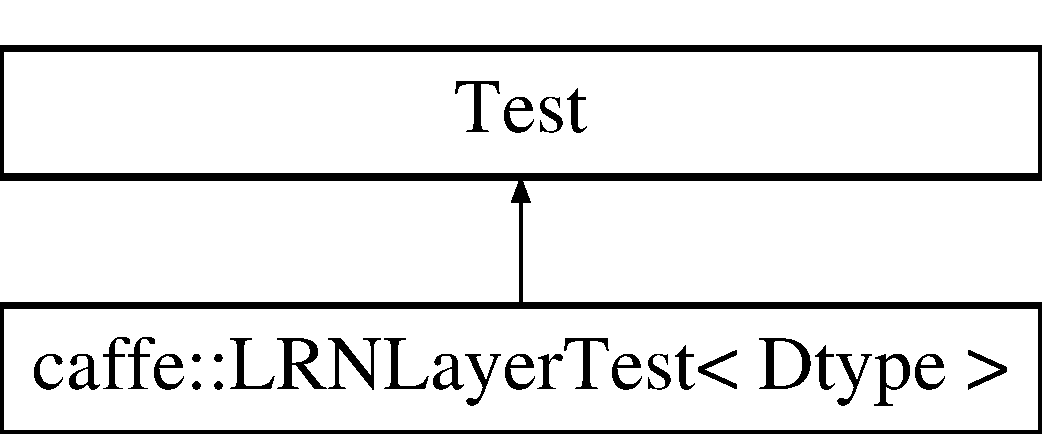
\includegraphics[height=2.000000cm]{classcaffe_1_1_l_r_n_layer_test}
\end{center}
\end{figure}
\subsection*{Protected Member Functions}
\begin{DoxyCompactItemize}
\item 
\hyperlink{classcaffe_1_1_l_r_n_layer_test_ace946d42913dc95ddac1b25ed5396088}{L\+R\+N\+Layer\+Test} ()
\item 
virtual void \hyperlink{classcaffe_1_1_l_r_n_layer_test_ad2523c7ee9662f281f49111b66080665}{Set\+Up} ()
\item 
virtual \hyperlink{classcaffe_1_1_l_r_n_layer_test_a5211067864feda1c496e684a8013c2dd}{$\sim$\+L\+R\+N\+Layer\+Test} ()
\item 
void \hyperlink{classcaffe_1_1_l_r_n_layer_test_a0a2026de787f7c723ede217b4312573c}{Reference\+L\+R\+N\+Forward} (const \hyperlink{classcaffe_1_1_blob}{Blob}$<$ Dtype $>$ \&blob\+\_\+bottom, const Layer\+Parameter \&layer\+\_\+param, \hyperlink{classcaffe_1_1_blob}{Blob}$<$ Dtype $>$ $\ast$blob\+\_\+top)
\end{DoxyCompactItemize}
\subsection*{Protected Attributes}
\begin{DoxyCompactItemize}
\item 
Dtype \hyperlink{classcaffe_1_1_l_r_n_layer_test_a9952e9353a5cb2c1155f17f315132f59}{epsilon\+\_\+}
\item 
\hyperlink{classcaffe_1_1_blob}{Blob}$<$ Dtype $>$ $\ast$const \hyperlink{classcaffe_1_1_l_r_n_layer_test_a14bf7b99347b9c3027faf75ea1a52ded}{blob\+\_\+bottom\+\_\+}
\item 
\hyperlink{classcaffe_1_1_blob}{Blob}$<$ Dtype $>$ $\ast$const \hyperlink{classcaffe_1_1_l_r_n_layer_test_a26ac20ad93eaec764e8595e84939964d}{blob\+\_\+top\+\_\+}
\item 
vector$<$ \hyperlink{classcaffe_1_1_blob}{Blob}$<$ Dtype $>$ $\ast$ $>$ \hyperlink{classcaffe_1_1_l_r_n_layer_test_a9c191aefd4a408d2a43035dd6015c1be}{blob\+\_\+bottom\+\_\+vec\+\_\+}
\item 
vector$<$ \hyperlink{classcaffe_1_1_blob}{Blob}$<$ Dtype $>$ $\ast$ $>$ \hyperlink{classcaffe_1_1_l_r_n_layer_test_aff3a0b8266c147b7922185b3153e7b68}{blob\+\_\+top\+\_\+vec\+\_\+}
\end{DoxyCompactItemize}


\subsection{Constructor \& Destructor Documentation}
\hypertarget{classcaffe_1_1_l_r_n_layer_test_ace946d42913dc95ddac1b25ed5396088}{\index{caffe\+::\+L\+R\+N\+Layer\+Test@{caffe\+::\+L\+R\+N\+Layer\+Test}!L\+R\+N\+Layer\+Test@{L\+R\+N\+Layer\+Test}}
\index{L\+R\+N\+Layer\+Test@{L\+R\+N\+Layer\+Test}!caffe\+::\+L\+R\+N\+Layer\+Test@{caffe\+::\+L\+R\+N\+Layer\+Test}}
\subsubsection[{L\+R\+N\+Layer\+Test}]{\setlength{\rightskip}{0pt plus 5cm}template$<$typename Dtype $>$ {\bf caffe\+::\+L\+R\+N\+Layer\+Test}$<$ Dtype $>$\+::{\bf L\+R\+N\+Layer\+Test} (
\begin{DoxyParamCaption}
{}
\end{DoxyParamCaption}
)\hspace{0.3cm}{\ttfamily [inline]}, {\ttfamily [protected]}}}\label{classcaffe_1_1_l_r_n_layer_test_ace946d42913dc95ddac1b25ed5396088}
\hypertarget{classcaffe_1_1_l_r_n_layer_test_a5211067864feda1c496e684a8013c2dd}{\index{caffe\+::\+L\+R\+N\+Layer\+Test@{caffe\+::\+L\+R\+N\+Layer\+Test}!````~L\+R\+N\+Layer\+Test@{$\sim$\+L\+R\+N\+Layer\+Test}}
\index{````~L\+R\+N\+Layer\+Test@{$\sim$\+L\+R\+N\+Layer\+Test}!caffe\+::\+L\+R\+N\+Layer\+Test@{caffe\+::\+L\+R\+N\+Layer\+Test}}
\subsubsection[{$\sim$\+L\+R\+N\+Layer\+Test}]{\setlength{\rightskip}{0pt plus 5cm}template$<$typename Dtype $>$ virtual {\bf caffe\+::\+L\+R\+N\+Layer\+Test}$<$ Dtype $>$\+::$\sim${\bf L\+R\+N\+Layer\+Test} (
\begin{DoxyParamCaption}
{}
\end{DoxyParamCaption}
)\hspace{0.3cm}{\ttfamily [inline]}, {\ttfamily [protected]}, {\ttfamily [virtual]}}}\label{classcaffe_1_1_l_r_n_layer_test_a5211067864feda1c496e684a8013c2dd}


\subsection{Member Function Documentation}
\hypertarget{classcaffe_1_1_l_r_n_layer_test_a0a2026de787f7c723ede217b4312573c}{\index{caffe\+::\+L\+R\+N\+Layer\+Test@{caffe\+::\+L\+R\+N\+Layer\+Test}!Reference\+L\+R\+N\+Forward@{Reference\+L\+R\+N\+Forward}}
\index{Reference\+L\+R\+N\+Forward@{Reference\+L\+R\+N\+Forward}!caffe\+::\+L\+R\+N\+Layer\+Test@{caffe\+::\+L\+R\+N\+Layer\+Test}}
\subsubsection[{Reference\+L\+R\+N\+Forward}]{\setlength{\rightskip}{0pt plus 5cm}template$<$typename Dtype $>$ void {\bf caffe\+::\+L\+R\+N\+Layer\+Test}$<$ Dtype $>$\+::Reference\+L\+R\+N\+Forward (
\begin{DoxyParamCaption}
\item[{const {\bf Blob}$<$ Dtype $>$ \&}]{blob\+\_\+bottom, }
\item[{const Layer\+Parameter \&}]{layer\+\_\+param, }
\item[{{\bf Blob}$<$ Dtype $>$ $\ast$}]{blob\+\_\+top}
\end{DoxyParamCaption}
)\hspace{0.3cm}{\ttfamily [protected]}}}\label{classcaffe_1_1_l_r_n_layer_test_a0a2026de787f7c723ede217b4312573c}
\hypertarget{classcaffe_1_1_l_r_n_layer_test_ad2523c7ee9662f281f49111b66080665}{\index{caffe\+::\+L\+R\+N\+Layer\+Test@{caffe\+::\+L\+R\+N\+Layer\+Test}!Set\+Up@{Set\+Up}}
\index{Set\+Up@{Set\+Up}!caffe\+::\+L\+R\+N\+Layer\+Test@{caffe\+::\+L\+R\+N\+Layer\+Test}}
\subsubsection[{Set\+Up}]{\setlength{\rightskip}{0pt plus 5cm}template$<$typename Dtype $>$ virtual void {\bf caffe\+::\+L\+R\+N\+Layer\+Test}$<$ Dtype $>$\+::Set\+Up (
\begin{DoxyParamCaption}
{}
\end{DoxyParamCaption}
)\hspace{0.3cm}{\ttfamily [inline]}, {\ttfamily [protected]}, {\ttfamily [virtual]}}}\label{classcaffe_1_1_l_r_n_layer_test_ad2523c7ee9662f281f49111b66080665}


\subsection{Member Data Documentation}
\hypertarget{classcaffe_1_1_l_r_n_layer_test_a14bf7b99347b9c3027faf75ea1a52ded}{\index{caffe\+::\+L\+R\+N\+Layer\+Test@{caffe\+::\+L\+R\+N\+Layer\+Test}!blob\+\_\+bottom\+\_\+@{blob\+\_\+bottom\+\_\+}}
\index{blob\+\_\+bottom\+\_\+@{blob\+\_\+bottom\+\_\+}!caffe\+::\+L\+R\+N\+Layer\+Test@{caffe\+::\+L\+R\+N\+Layer\+Test}}
\subsubsection[{blob\+\_\+bottom\+\_\+}]{\setlength{\rightskip}{0pt plus 5cm}template$<$typename Dtype $>$ {\bf Blob}$<$Dtype$>$$\ast$ const {\bf caffe\+::\+L\+R\+N\+Layer\+Test}$<$ Dtype $>$\+::blob\+\_\+bottom\+\_\+\hspace{0.3cm}{\ttfamily [protected]}}}\label{classcaffe_1_1_l_r_n_layer_test_a14bf7b99347b9c3027faf75ea1a52ded}
\hypertarget{classcaffe_1_1_l_r_n_layer_test_a9c191aefd4a408d2a43035dd6015c1be}{\index{caffe\+::\+L\+R\+N\+Layer\+Test@{caffe\+::\+L\+R\+N\+Layer\+Test}!blob\+\_\+bottom\+\_\+vec\+\_\+@{blob\+\_\+bottom\+\_\+vec\+\_\+}}
\index{blob\+\_\+bottom\+\_\+vec\+\_\+@{blob\+\_\+bottom\+\_\+vec\+\_\+}!caffe\+::\+L\+R\+N\+Layer\+Test@{caffe\+::\+L\+R\+N\+Layer\+Test}}
\subsubsection[{blob\+\_\+bottom\+\_\+vec\+\_\+}]{\setlength{\rightskip}{0pt plus 5cm}template$<$typename Dtype $>$ vector$<${\bf Blob}$<$Dtype$>$$\ast$$>$ {\bf caffe\+::\+L\+R\+N\+Layer\+Test}$<$ Dtype $>$\+::blob\+\_\+bottom\+\_\+vec\+\_\+\hspace{0.3cm}{\ttfamily [protected]}}}\label{classcaffe_1_1_l_r_n_layer_test_a9c191aefd4a408d2a43035dd6015c1be}
\hypertarget{classcaffe_1_1_l_r_n_layer_test_a26ac20ad93eaec764e8595e84939964d}{\index{caffe\+::\+L\+R\+N\+Layer\+Test@{caffe\+::\+L\+R\+N\+Layer\+Test}!blob\+\_\+top\+\_\+@{blob\+\_\+top\+\_\+}}
\index{blob\+\_\+top\+\_\+@{blob\+\_\+top\+\_\+}!caffe\+::\+L\+R\+N\+Layer\+Test@{caffe\+::\+L\+R\+N\+Layer\+Test}}
\subsubsection[{blob\+\_\+top\+\_\+}]{\setlength{\rightskip}{0pt plus 5cm}template$<$typename Dtype $>$ {\bf Blob}$<$Dtype$>$$\ast$ const {\bf caffe\+::\+L\+R\+N\+Layer\+Test}$<$ Dtype $>$\+::blob\+\_\+top\+\_\+\hspace{0.3cm}{\ttfamily [protected]}}}\label{classcaffe_1_1_l_r_n_layer_test_a26ac20ad93eaec764e8595e84939964d}
\hypertarget{classcaffe_1_1_l_r_n_layer_test_aff3a0b8266c147b7922185b3153e7b68}{\index{caffe\+::\+L\+R\+N\+Layer\+Test@{caffe\+::\+L\+R\+N\+Layer\+Test}!blob\+\_\+top\+\_\+vec\+\_\+@{blob\+\_\+top\+\_\+vec\+\_\+}}
\index{blob\+\_\+top\+\_\+vec\+\_\+@{blob\+\_\+top\+\_\+vec\+\_\+}!caffe\+::\+L\+R\+N\+Layer\+Test@{caffe\+::\+L\+R\+N\+Layer\+Test}}
\subsubsection[{blob\+\_\+top\+\_\+vec\+\_\+}]{\setlength{\rightskip}{0pt plus 5cm}template$<$typename Dtype $>$ vector$<${\bf Blob}$<$Dtype$>$$\ast$$>$ {\bf caffe\+::\+L\+R\+N\+Layer\+Test}$<$ Dtype $>$\+::blob\+\_\+top\+\_\+vec\+\_\+\hspace{0.3cm}{\ttfamily [protected]}}}\label{classcaffe_1_1_l_r_n_layer_test_aff3a0b8266c147b7922185b3153e7b68}
\hypertarget{classcaffe_1_1_l_r_n_layer_test_a9952e9353a5cb2c1155f17f315132f59}{\index{caffe\+::\+L\+R\+N\+Layer\+Test@{caffe\+::\+L\+R\+N\+Layer\+Test}!epsilon\+\_\+@{epsilon\+\_\+}}
\index{epsilon\+\_\+@{epsilon\+\_\+}!caffe\+::\+L\+R\+N\+Layer\+Test@{caffe\+::\+L\+R\+N\+Layer\+Test}}
\subsubsection[{epsilon\+\_\+}]{\setlength{\rightskip}{0pt plus 5cm}template$<$typename Dtype $>$ Dtype {\bf caffe\+::\+L\+R\+N\+Layer\+Test}$<$ Dtype $>$\+::epsilon\+\_\+\hspace{0.3cm}{\ttfamily [protected]}}}\label{classcaffe_1_1_l_r_n_layer_test_a9952e9353a5cb2c1155f17f315132f59}


The documentation for this class was generated from the following file\+:\begin{DoxyCompactItemize}
\item 
src/caffe/test/\hyperlink{test__lrn__layer_8cpp}{test\+\_\+lrn\+\_\+layer.\+cpp}\end{DoxyCompactItemize}

\hypertarget{classcaffe_1_1_math_functions_test}{\section{caffe\+:\+:Math\+Functions\+Test$<$ Dtype $>$ Class Template Reference}
\label{classcaffe_1_1_math_functions_test}\index{caffe\+::\+Math\+Functions\+Test$<$ Dtype $>$@{caffe\+::\+Math\+Functions\+Test$<$ Dtype $>$}}
}
Inheritance diagram for caffe\+:\+:Math\+Functions\+Test$<$ Dtype $>$\+:\begin{figure}[H]
\begin{center}
\leavevmode
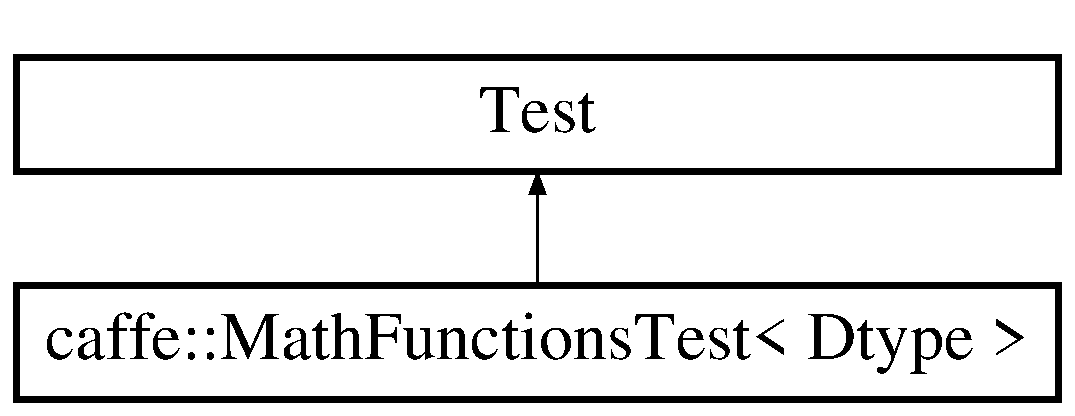
\includegraphics[height=2.000000cm]{classcaffe_1_1_math_functions_test}
\end{center}
\end{figure}
\subsection*{Protected Member Functions}
\begin{DoxyCompactItemize}
\item 
\hyperlink{classcaffe_1_1_math_functions_test_afc888e08659197a2127f87c5f6194e55}{Math\+Functions\+Test} ()
\item 
virtual void \hyperlink{classcaffe_1_1_math_functions_test_a93b8a67e99e6f975bf539daf193b1a8e}{Set\+Up} ()
\item 
virtual \hyperlink{classcaffe_1_1_math_functions_test_ab071770d4f515a095093b2cf3e718df3}{$\sim$\+Math\+Functions\+Test} ()
\item 
int \hyperlink{classcaffe_1_1_math_functions_test_a6c8c13893f7ab3b5e38ebc50226862bc}{Reference\+Hamming\+Distance} (const int n, const Dtype $\ast$x, const Dtype $\ast$y)
\end{DoxyCompactItemize}
\subsection*{Protected Attributes}
\begin{DoxyCompactItemize}
\item 
\hyperlink{classcaffe_1_1_blob}{Blob}$<$ Dtype $>$ $\ast$const \hyperlink{classcaffe_1_1_math_functions_test_acd87accc66124e064d86484a4213afd8}{blob\+\_\+bottom\+\_\+}
\item 
\hyperlink{classcaffe_1_1_blob}{Blob}$<$ Dtype $>$ $\ast$const \hyperlink{classcaffe_1_1_math_functions_test_a260c2e90738ed8b2d66e18f7589ffef0}{blob\+\_\+top\+\_\+}
\end{DoxyCompactItemize}


\subsection{Constructor \& Destructor Documentation}
\hypertarget{classcaffe_1_1_math_functions_test_afc888e08659197a2127f87c5f6194e55}{\index{caffe\+::\+Math\+Functions\+Test@{caffe\+::\+Math\+Functions\+Test}!Math\+Functions\+Test@{Math\+Functions\+Test}}
\index{Math\+Functions\+Test@{Math\+Functions\+Test}!caffe\+::\+Math\+Functions\+Test@{caffe\+::\+Math\+Functions\+Test}}
\subsubsection[{Math\+Functions\+Test}]{\setlength{\rightskip}{0pt plus 5cm}template$<$typename Dtype $>$ {\bf caffe\+::\+Math\+Functions\+Test}$<$ Dtype $>$\+::{\bf Math\+Functions\+Test} (
\begin{DoxyParamCaption}
{}
\end{DoxyParamCaption}
)\hspace{0.3cm}{\ttfamily [inline]}, {\ttfamily [protected]}}}\label{classcaffe_1_1_math_functions_test_afc888e08659197a2127f87c5f6194e55}
\hypertarget{classcaffe_1_1_math_functions_test_ab071770d4f515a095093b2cf3e718df3}{\index{caffe\+::\+Math\+Functions\+Test@{caffe\+::\+Math\+Functions\+Test}!````~Math\+Functions\+Test@{$\sim$\+Math\+Functions\+Test}}
\index{````~Math\+Functions\+Test@{$\sim$\+Math\+Functions\+Test}!caffe\+::\+Math\+Functions\+Test@{caffe\+::\+Math\+Functions\+Test}}
\subsubsection[{$\sim$\+Math\+Functions\+Test}]{\setlength{\rightskip}{0pt plus 5cm}template$<$typename Dtype $>$ virtual {\bf caffe\+::\+Math\+Functions\+Test}$<$ Dtype $>$\+::$\sim${\bf Math\+Functions\+Test} (
\begin{DoxyParamCaption}
{}
\end{DoxyParamCaption}
)\hspace{0.3cm}{\ttfamily [inline]}, {\ttfamily [protected]}, {\ttfamily [virtual]}}}\label{classcaffe_1_1_math_functions_test_ab071770d4f515a095093b2cf3e718df3}


\subsection{Member Function Documentation}
\hypertarget{classcaffe_1_1_math_functions_test_a6c8c13893f7ab3b5e38ebc50226862bc}{\index{caffe\+::\+Math\+Functions\+Test@{caffe\+::\+Math\+Functions\+Test}!Reference\+Hamming\+Distance@{Reference\+Hamming\+Distance}}
\index{Reference\+Hamming\+Distance@{Reference\+Hamming\+Distance}!caffe\+::\+Math\+Functions\+Test@{caffe\+::\+Math\+Functions\+Test}}
\subsubsection[{Reference\+Hamming\+Distance}]{\setlength{\rightskip}{0pt plus 5cm}template$<$typename Dtype $>$ int {\bf caffe\+::\+Math\+Functions\+Test}$<$ Dtype $>$\+::Reference\+Hamming\+Distance (
\begin{DoxyParamCaption}
\item[{const int}]{n, }
\item[{const Dtype $\ast$}]{x, }
\item[{const Dtype $\ast$}]{y}
\end{DoxyParamCaption}
)\hspace{0.3cm}{\ttfamily [inline]}, {\ttfamily [protected]}}}\label{classcaffe_1_1_math_functions_test_a6c8c13893f7ab3b5e38ebc50226862bc}
\hypertarget{classcaffe_1_1_math_functions_test_a93b8a67e99e6f975bf539daf193b1a8e}{\index{caffe\+::\+Math\+Functions\+Test@{caffe\+::\+Math\+Functions\+Test}!Set\+Up@{Set\+Up}}
\index{Set\+Up@{Set\+Up}!caffe\+::\+Math\+Functions\+Test@{caffe\+::\+Math\+Functions\+Test}}
\subsubsection[{Set\+Up}]{\setlength{\rightskip}{0pt plus 5cm}template$<$typename Dtype $>$ virtual void {\bf caffe\+::\+Math\+Functions\+Test}$<$ Dtype $>$\+::Set\+Up (
\begin{DoxyParamCaption}
{}
\end{DoxyParamCaption}
)\hspace{0.3cm}{\ttfamily [inline]}, {\ttfamily [protected]}, {\ttfamily [virtual]}}}\label{classcaffe_1_1_math_functions_test_a93b8a67e99e6f975bf539daf193b1a8e}


\subsection{Member Data Documentation}
\hypertarget{classcaffe_1_1_math_functions_test_acd87accc66124e064d86484a4213afd8}{\index{caffe\+::\+Math\+Functions\+Test@{caffe\+::\+Math\+Functions\+Test}!blob\+\_\+bottom\+\_\+@{blob\+\_\+bottom\+\_\+}}
\index{blob\+\_\+bottom\+\_\+@{blob\+\_\+bottom\+\_\+}!caffe\+::\+Math\+Functions\+Test@{caffe\+::\+Math\+Functions\+Test}}
\subsubsection[{blob\+\_\+bottom\+\_\+}]{\setlength{\rightskip}{0pt plus 5cm}template$<$typename Dtype $>$ {\bf Blob}$<$Dtype$>$$\ast$ const {\bf caffe\+::\+Math\+Functions\+Test}$<$ Dtype $>$\+::blob\+\_\+bottom\+\_\+\hspace{0.3cm}{\ttfamily [protected]}}}\label{classcaffe_1_1_math_functions_test_acd87accc66124e064d86484a4213afd8}
\hypertarget{classcaffe_1_1_math_functions_test_a260c2e90738ed8b2d66e18f7589ffef0}{\index{caffe\+::\+Math\+Functions\+Test@{caffe\+::\+Math\+Functions\+Test}!blob\+\_\+top\+\_\+@{blob\+\_\+top\+\_\+}}
\index{blob\+\_\+top\+\_\+@{blob\+\_\+top\+\_\+}!caffe\+::\+Math\+Functions\+Test@{caffe\+::\+Math\+Functions\+Test}}
\subsubsection[{blob\+\_\+top\+\_\+}]{\setlength{\rightskip}{0pt plus 5cm}template$<$typename Dtype $>$ {\bf Blob}$<$Dtype$>$$\ast$ const {\bf caffe\+::\+Math\+Functions\+Test}$<$ Dtype $>$\+::blob\+\_\+top\+\_\+\hspace{0.3cm}{\ttfamily [protected]}}}\label{classcaffe_1_1_math_functions_test_a260c2e90738ed8b2d66e18f7589ffef0}


The documentation for this class was generated from the following file\+:\begin{DoxyCompactItemize}
\item 
src/caffe/test/\hyperlink{test__math__functions_8cpp}{test\+\_\+math\+\_\+functions.\+cpp}\end{DoxyCompactItemize}

\hypertarget{classcaffe_1_1_memory_data_layer}{\section{caffe\+:\+:Memory\+Data\+Layer$<$ Dtype $>$ Class Template Reference}
\label{classcaffe_1_1_memory_data_layer}\index{caffe\+::\+Memory\+Data\+Layer$<$ Dtype $>$@{caffe\+::\+Memory\+Data\+Layer$<$ Dtype $>$}}
}


{\ttfamily \#include $<$vision\+\_\+layers.\+hpp$>$}

Inheritance diagram for caffe\+:\+:Memory\+Data\+Layer$<$ Dtype $>$\+:\begin{figure}[H]
\begin{center}
\leavevmode
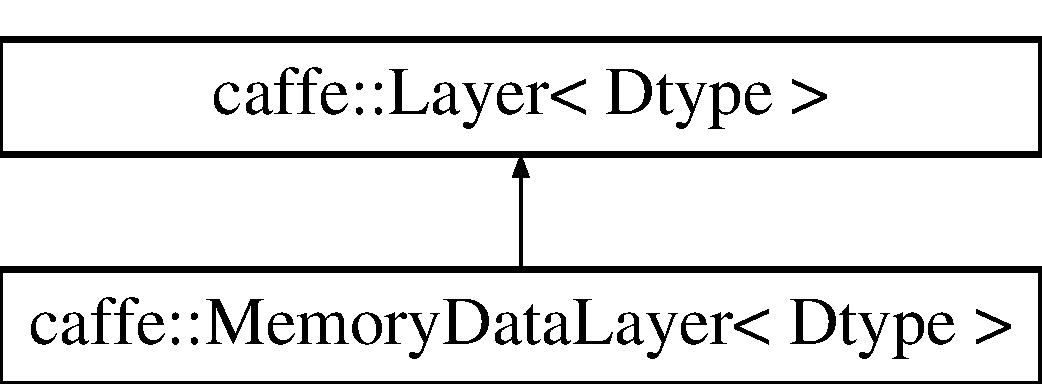
\includegraphics[height=2.000000cm]{classcaffe_1_1_memory_data_layer}
\end{center}
\end{figure}
\subsection*{Public Member Functions}
\begin{DoxyCompactItemize}
\item 
\hyperlink{classcaffe_1_1_memory_data_layer_a9bf012786068bfe846694af129a6736f}{Memory\+Data\+Layer} (const Layer\+Parameter \&param)
\item 
virtual void \hyperlink{classcaffe_1_1_memory_data_layer_a276f9246a9ff0e6f016dfb54f00da88d}{Set\+Up} (const vector$<$ \hyperlink{classcaffe_1_1_blob}{Blob}$<$ Dtype $>$ $\ast$ $>$ \&bottom, vector$<$ \hyperlink{classcaffe_1_1_blob}{Blob}$<$ Dtype $>$ $\ast$ $>$ $\ast$top)
\item 
void \hyperlink{classcaffe_1_1_memory_data_layer_aeaa745c4fe3a957b973bf94dca6a5f2b}{Reset} (Dtype $\ast$data, Dtype $\ast$label, int n)
\item 
int \hyperlink{classcaffe_1_1_memory_data_layer_ab8d57e0648185469a8883fd77cce5c2c}{datum\+\_\+channels} ()
\item 
int \hyperlink{classcaffe_1_1_memory_data_layer_aa60a2e9729fdd79ec46daaa3ace1717d}{datum\+\_\+height} ()
\item 
int \hyperlink{classcaffe_1_1_memory_data_layer_addc2b736e9e4a80e360c86ded1bc01de}{datum\+\_\+width} ()
\item 
int \hyperlink{classcaffe_1_1_memory_data_layer_a06bfb6d06f61db11699a6b3ce7b1ee53}{batch\+\_\+size} ()
\end{DoxyCompactItemize}
\subsection*{Protected Member Functions}
\begin{DoxyCompactItemize}
\item 
virtual Dtype \hyperlink{classcaffe_1_1_memory_data_layer_a124ae7ed94f0cad8a7c64b3c4b79eb33}{Forward\+\_\+cpu} (const vector$<$ \hyperlink{classcaffe_1_1_blob}{Blob}$<$ Dtype $>$ $\ast$ $>$ \&bottom, vector$<$ \hyperlink{classcaffe_1_1_blob}{Blob}$<$ Dtype $>$ $\ast$ $>$ $\ast$top)
\item 
virtual void \hyperlink{classcaffe_1_1_memory_data_layer_ac85916554558f0ca7881bd3ee608865c}{Backward\+\_\+cpu} (const vector$<$ \hyperlink{classcaffe_1_1_blob}{Blob}$<$ Dtype $>$ $\ast$ $>$ \&top, const bool propagate\+\_\+down, vector$<$ \hyperlink{classcaffe_1_1_blob}{Blob}$<$ Dtype $>$ $\ast$ $>$ $\ast$bottom)
\item 
virtual void \hyperlink{classcaffe_1_1_memory_data_layer_ab209891a982c0962c78c36dedf2916ed}{Backward\+\_\+gpu} (const vector$<$ \hyperlink{classcaffe_1_1_blob}{Blob}$<$ Dtype $>$ $\ast$ $>$ \&top, const bool propagate\+\_\+down, vector$<$ \hyperlink{classcaffe_1_1_blob}{Blob}$<$ Dtype $>$ $\ast$ $>$ $\ast$bottom)
\end{DoxyCompactItemize}
\subsection*{Protected Attributes}
\begin{DoxyCompactItemize}
\item 
Dtype $\ast$ \hyperlink{classcaffe_1_1_memory_data_layer_a57a7e3dca84db2b07cb009a44c6ae45c}{data\+\_\+}
\item 
Dtype $\ast$ \hyperlink{classcaffe_1_1_memory_data_layer_abf7f9a81ae3268a6eea7fbd97760e28a}{labels\+\_\+}
\item 
int \hyperlink{classcaffe_1_1_memory_data_layer_ae77bcb4c0f6183477f264438c90fe6b6}{datum\+\_\+channels\+\_\+}
\item 
int \hyperlink{classcaffe_1_1_memory_data_layer_a7a72970c6c500580c0b889dbb492aa9e}{datum\+\_\+height\+\_\+}
\item 
int \hyperlink{classcaffe_1_1_memory_data_layer_ac11837cf9ad597efdae80110c328df80}{datum\+\_\+width\+\_\+}
\item 
int \hyperlink{classcaffe_1_1_memory_data_layer_ae402a79948a2f545139c45c0d48fd45a}{datum\+\_\+size\+\_\+}
\item 
int \hyperlink{classcaffe_1_1_memory_data_layer_a94335b05660c950a4ba711342daff276}{batch\+\_\+size\+\_\+}
\item 
int \hyperlink{classcaffe_1_1_memory_data_layer_a303b19a435878a94ede0c8e1fb26f2a1}{n\+\_\+}
\item 
int \hyperlink{classcaffe_1_1_memory_data_layer_a21694a78bc84c9cedae58e66ee542a5b}{pos\+\_\+}
\end{DoxyCompactItemize}


\subsection{Constructor \& Destructor Documentation}
\hypertarget{classcaffe_1_1_memory_data_layer_a9bf012786068bfe846694af129a6736f}{\index{caffe\+::\+Memory\+Data\+Layer@{caffe\+::\+Memory\+Data\+Layer}!Memory\+Data\+Layer@{Memory\+Data\+Layer}}
\index{Memory\+Data\+Layer@{Memory\+Data\+Layer}!caffe\+::\+Memory\+Data\+Layer@{caffe\+::\+Memory\+Data\+Layer}}
\subsubsection[{Memory\+Data\+Layer}]{\setlength{\rightskip}{0pt plus 5cm}template$<$typename Dtype $>$ {\bf caffe\+::\+Memory\+Data\+Layer}$<$ Dtype $>$\+::{\bf Memory\+Data\+Layer} (
\begin{DoxyParamCaption}
\item[{const Layer\+Parameter \&}]{param}
\end{DoxyParamCaption}
)\hspace{0.3cm}{\ttfamily [inline]}, {\ttfamily [explicit]}}}\label{classcaffe_1_1_memory_data_layer_a9bf012786068bfe846694af129a6736f}


\subsection{Member Function Documentation}
\hypertarget{classcaffe_1_1_memory_data_layer_ac85916554558f0ca7881bd3ee608865c}{\index{caffe\+::\+Memory\+Data\+Layer@{caffe\+::\+Memory\+Data\+Layer}!Backward\+\_\+cpu@{Backward\+\_\+cpu}}
\index{Backward\+\_\+cpu@{Backward\+\_\+cpu}!caffe\+::\+Memory\+Data\+Layer@{caffe\+::\+Memory\+Data\+Layer}}
\subsubsection[{Backward\+\_\+cpu}]{\setlength{\rightskip}{0pt plus 5cm}template$<$typename Dtype $>$ virtual void {\bf caffe\+::\+Memory\+Data\+Layer}$<$ Dtype $>$\+::Backward\+\_\+cpu (
\begin{DoxyParamCaption}
\item[{const vector$<$ {\bf Blob}$<$ Dtype $>$ $\ast$ $>$ \&}]{top, }
\item[{const bool}]{propagate\+\_\+down, }
\item[{vector$<$ {\bf Blob}$<$ Dtype $>$ $\ast$ $>$ $\ast$}]{bottom}
\end{DoxyParamCaption}
)\hspace{0.3cm}{\ttfamily [inline]}, {\ttfamily [protected]}, {\ttfamily [virtual]}}}\label{classcaffe_1_1_memory_data_layer_ac85916554558f0ca7881bd3ee608865c}


Implements \hyperlink{classcaffe_1_1_layer_ac2d82011d076237c67997f63e7ee4b80}{caffe\+::\+Layer$<$ Dtype $>$}.

\hypertarget{classcaffe_1_1_memory_data_layer_ab209891a982c0962c78c36dedf2916ed}{\index{caffe\+::\+Memory\+Data\+Layer@{caffe\+::\+Memory\+Data\+Layer}!Backward\+\_\+gpu@{Backward\+\_\+gpu}}
\index{Backward\+\_\+gpu@{Backward\+\_\+gpu}!caffe\+::\+Memory\+Data\+Layer@{caffe\+::\+Memory\+Data\+Layer}}
\subsubsection[{Backward\+\_\+gpu}]{\setlength{\rightskip}{0pt plus 5cm}template$<$typename Dtype $>$ virtual void {\bf caffe\+::\+Memory\+Data\+Layer}$<$ Dtype $>$\+::Backward\+\_\+gpu (
\begin{DoxyParamCaption}
\item[{const vector$<$ {\bf Blob}$<$ Dtype $>$ $\ast$ $>$ \&}]{top, }
\item[{const bool}]{propagate\+\_\+down, }
\item[{vector$<$ {\bf Blob}$<$ Dtype $>$ $\ast$ $>$ $\ast$}]{bottom}
\end{DoxyParamCaption}
)\hspace{0.3cm}{\ttfamily [inline]}, {\ttfamily [protected]}, {\ttfamily [virtual]}}}\label{classcaffe_1_1_memory_data_layer_ab209891a982c0962c78c36dedf2916ed}


Reimplemented from \hyperlink{classcaffe_1_1_layer_adf07ffe1f22d2fd2b1b0ff475ef5a64b}{caffe\+::\+Layer$<$ Dtype $>$}.

\hypertarget{classcaffe_1_1_memory_data_layer_a06bfb6d06f61db11699a6b3ce7b1ee53}{\index{caffe\+::\+Memory\+Data\+Layer@{caffe\+::\+Memory\+Data\+Layer}!batch\+\_\+size@{batch\+\_\+size}}
\index{batch\+\_\+size@{batch\+\_\+size}!caffe\+::\+Memory\+Data\+Layer@{caffe\+::\+Memory\+Data\+Layer}}
\subsubsection[{batch\+\_\+size}]{\setlength{\rightskip}{0pt plus 5cm}template$<$typename Dtype $>$ int {\bf caffe\+::\+Memory\+Data\+Layer}$<$ Dtype $>$\+::batch\+\_\+size (
\begin{DoxyParamCaption}
{}
\end{DoxyParamCaption}
)\hspace{0.3cm}{\ttfamily [inline]}}}\label{classcaffe_1_1_memory_data_layer_a06bfb6d06f61db11699a6b3ce7b1ee53}
\hypertarget{classcaffe_1_1_memory_data_layer_ab8d57e0648185469a8883fd77cce5c2c}{\index{caffe\+::\+Memory\+Data\+Layer@{caffe\+::\+Memory\+Data\+Layer}!datum\+\_\+channels@{datum\+\_\+channels}}
\index{datum\+\_\+channels@{datum\+\_\+channels}!caffe\+::\+Memory\+Data\+Layer@{caffe\+::\+Memory\+Data\+Layer}}
\subsubsection[{datum\+\_\+channels}]{\setlength{\rightskip}{0pt plus 5cm}template$<$typename Dtype $>$ int {\bf caffe\+::\+Memory\+Data\+Layer}$<$ Dtype $>$\+::datum\+\_\+channels (
\begin{DoxyParamCaption}
{}
\end{DoxyParamCaption}
)\hspace{0.3cm}{\ttfamily [inline]}}}\label{classcaffe_1_1_memory_data_layer_ab8d57e0648185469a8883fd77cce5c2c}
\hypertarget{classcaffe_1_1_memory_data_layer_aa60a2e9729fdd79ec46daaa3ace1717d}{\index{caffe\+::\+Memory\+Data\+Layer@{caffe\+::\+Memory\+Data\+Layer}!datum\+\_\+height@{datum\+\_\+height}}
\index{datum\+\_\+height@{datum\+\_\+height}!caffe\+::\+Memory\+Data\+Layer@{caffe\+::\+Memory\+Data\+Layer}}
\subsubsection[{datum\+\_\+height}]{\setlength{\rightskip}{0pt plus 5cm}template$<$typename Dtype $>$ int {\bf caffe\+::\+Memory\+Data\+Layer}$<$ Dtype $>$\+::datum\+\_\+height (
\begin{DoxyParamCaption}
{}
\end{DoxyParamCaption}
)\hspace{0.3cm}{\ttfamily [inline]}}}\label{classcaffe_1_1_memory_data_layer_aa60a2e9729fdd79ec46daaa3ace1717d}
\hypertarget{classcaffe_1_1_memory_data_layer_addc2b736e9e4a80e360c86ded1bc01de}{\index{caffe\+::\+Memory\+Data\+Layer@{caffe\+::\+Memory\+Data\+Layer}!datum\+\_\+width@{datum\+\_\+width}}
\index{datum\+\_\+width@{datum\+\_\+width}!caffe\+::\+Memory\+Data\+Layer@{caffe\+::\+Memory\+Data\+Layer}}
\subsubsection[{datum\+\_\+width}]{\setlength{\rightskip}{0pt plus 5cm}template$<$typename Dtype $>$ int {\bf caffe\+::\+Memory\+Data\+Layer}$<$ Dtype $>$\+::datum\+\_\+width (
\begin{DoxyParamCaption}
{}
\end{DoxyParamCaption}
)\hspace{0.3cm}{\ttfamily [inline]}}}\label{classcaffe_1_1_memory_data_layer_addc2b736e9e4a80e360c86ded1bc01de}
\hypertarget{classcaffe_1_1_memory_data_layer_a124ae7ed94f0cad8a7c64b3c4b79eb33}{\index{caffe\+::\+Memory\+Data\+Layer@{caffe\+::\+Memory\+Data\+Layer}!Forward\+\_\+cpu@{Forward\+\_\+cpu}}
\index{Forward\+\_\+cpu@{Forward\+\_\+cpu}!caffe\+::\+Memory\+Data\+Layer@{caffe\+::\+Memory\+Data\+Layer}}
\subsubsection[{Forward\+\_\+cpu}]{\setlength{\rightskip}{0pt plus 5cm}template$<$typename Dtype $>$ Dtype {\bf caffe\+::\+Memory\+Data\+Layer}$<$ Dtype $>$\+::Forward\+\_\+cpu (
\begin{DoxyParamCaption}
\item[{const vector$<$ {\bf Blob}$<$ Dtype $>$ $\ast$ $>$ \&}]{bottom, }
\item[{vector$<$ {\bf Blob}$<$ Dtype $>$ $\ast$ $>$ $\ast$}]{top}
\end{DoxyParamCaption}
)\hspace{0.3cm}{\ttfamily [protected]}, {\ttfamily [virtual]}}}\label{classcaffe_1_1_memory_data_layer_a124ae7ed94f0cad8a7c64b3c4b79eb33}


Implements \hyperlink{classcaffe_1_1_layer_a8f7f61da3b8b3ca7f2394dee33873353}{caffe\+::\+Layer$<$ Dtype $>$}.

\hypertarget{classcaffe_1_1_memory_data_layer_aeaa745c4fe3a957b973bf94dca6a5f2b}{\index{caffe\+::\+Memory\+Data\+Layer@{caffe\+::\+Memory\+Data\+Layer}!Reset@{Reset}}
\index{Reset@{Reset}!caffe\+::\+Memory\+Data\+Layer@{caffe\+::\+Memory\+Data\+Layer}}
\subsubsection[{Reset}]{\setlength{\rightskip}{0pt plus 5cm}template$<$typename Dtype $>$ void {\bf caffe\+::\+Memory\+Data\+Layer}$<$ Dtype $>$\+::Reset (
\begin{DoxyParamCaption}
\item[{Dtype $\ast$}]{data, }
\item[{Dtype $\ast$}]{label, }
\item[{int}]{n}
\end{DoxyParamCaption}
)}}\label{classcaffe_1_1_memory_data_layer_aeaa745c4fe3a957b973bf94dca6a5f2b}
\hypertarget{classcaffe_1_1_memory_data_layer_a276f9246a9ff0e6f016dfb54f00da88d}{\index{caffe\+::\+Memory\+Data\+Layer@{caffe\+::\+Memory\+Data\+Layer}!Set\+Up@{Set\+Up}}
\index{Set\+Up@{Set\+Up}!caffe\+::\+Memory\+Data\+Layer@{caffe\+::\+Memory\+Data\+Layer}}
\subsubsection[{Set\+Up}]{\setlength{\rightskip}{0pt plus 5cm}template$<$typename Dtype $>$ void {\bf caffe\+::\+Memory\+Data\+Layer}$<$ Dtype $>$\+::Set\+Up (
\begin{DoxyParamCaption}
\item[{const vector$<$ {\bf Blob}$<$ Dtype $>$ $\ast$ $>$ \&}]{bottom, }
\item[{vector$<$ {\bf Blob}$<$ Dtype $>$ $\ast$ $>$ $\ast$}]{top}
\end{DoxyParamCaption}
)\hspace{0.3cm}{\ttfamily [virtual]}}}\label{classcaffe_1_1_memory_data_layer_a276f9246a9ff0e6f016dfb54f00da88d}


Implements \hyperlink{classcaffe_1_1_layer_abd13c6489c13953b4fbcfcf6880835d0}{caffe\+::\+Layer$<$ Dtype $>$}.



\subsection{Member Data Documentation}
\hypertarget{classcaffe_1_1_memory_data_layer_a94335b05660c950a4ba711342daff276}{\index{caffe\+::\+Memory\+Data\+Layer@{caffe\+::\+Memory\+Data\+Layer}!batch\+\_\+size\+\_\+@{batch\+\_\+size\+\_\+}}
\index{batch\+\_\+size\+\_\+@{batch\+\_\+size\+\_\+}!caffe\+::\+Memory\+Data\+Layer@{caffe\+::\+Memory\+Data\+Layer}}
\subsubsection[{batch\+\_\+size\+\_\+}]{\setlength{\rightskip}{0pt plus 5cm}template$<$typename Dtype $>$ int {\bf caffe\+::\+Memory\+Data\+Layer}$<$ Dtype $>$\+::batch\+\_\+size\+\_\+\hspace{0.3cm}{\ttfamily [protected]}}}\label{classcaffe_1_1_memory_data_layer_a94335b05660c950a4ba711342daff276}
\hypertarget{classcaffe_1_1_memory_data_layer_a57a7e3dca84db2b07cb009a44c6ae45c}{\index{caffe\+::\+Memory\+Data\+Layer@{caffe\+::\+Memory\+Data\+Layer}!data\+\_\+@{data\+\_\+}}
\index{data\+\_\+@{data\+\_\+}!caffe\+::\+Memory\+Data\+Layer@{caffe\+::\+Memory\+Data\+Layer}}
\subsubsection[{data\+\_\+}]{\setlength{\rightskip}{0pt plus 5cm}template$<$typename Dtype $>$ Dtype$\ast$ {\bf caffe\+::\+Memory\+Data\+Layer}$<$ Dtype $>$\+::data\+\_\+\hspace{0.3cm}{\ttfamily [protected]}}}\label{classcaffe_1_1_memory_data_layer_a57a7e3dca84db2b07cb009a44c6ae45c}
\hypertarget{classcaffe_1_1_memory_data_layer_ae77bcb4c0f6183477f264438c90fe6b6}{\index{caffe\+::\+Memory\+Data\+Layer@{caffe\+::\+Memory\+Data\+Layer}!datum\+\_\+channels\+\_\+@{datum\+\_\+channels\+\_\+}}
\index{datum\+\_\+channels\+\_\+@{datum\+\_\+channels\+\_\+}!caffe\+::\+Memory\+Data\+Layer@{caffe\+::\+Memory\+Data\+Layer}}
\subsubsection[{datum\+\_\+channels\+\_\+}]{\setlength{\rightskip}{0pt plus 5cm}template$<$typename Dtype $>$ int {\bf caffe\+::\+Memory\+Data\+Layer}$<$ Dtype $>$\+::datum\+\_\+channels\+\_\+\hspace{0.3cm}{\ttfamily [protected]}}}\label{classcaffe_1_1_memory_data_layer_ae77bcb4c0f6183477f264438c90fe6b6}
\hypertarget{classcaffe_1_1_memory_data_layer_a7a72970c6c500580c0b889dbb492aa9e}{\index{caffe\+::\+Memory\+Data\+Layer@{caffe\+::\+Memory\+Data\+Layer}!datum\+\_\+height\+\_\+@{datum\+\_\+height\+\_\+}}
\index{datum\+\_\+height\+\_\+@{datum\+\_\+height\+\_\+}!caffe\+::\+Memory\+Data\+Layer@{caffe\+::\+Memory\+Data\+Layer}}
\subsubsection[{datum\+\_\+height\+\_\+}]{\setlength{\rightskip}{0pt plus 5cm}template$<$typename Dtype $>$ int {\bf caffe\+::\+Memory\+Data\+Layer}$<$ Dtype $>$\+::datum\+\_\+height\+\_\+\hspace{0.3cm}{\ttfamily [protected]}}}\label{classcaffe_1_1_memory_data_layer_a7a72970c6c500580c0b889dbb492aa9e}
\hypertarget{classcaffe_1_1_memory_data_layer_ae402a79948a2f545139c45c0d48fd45a}{\index{caffe\+::\+Memory\+Data\+Layer@{caffe\+::\+Memory\+Data\+Layer}!datum\+\_\+size\+\_\+@{datum\+\_\+size\+\_\+}}
\index{datum\+\_\+size\+\_\+@{datum\+\_\+size\+\_\+}!caffe\+::\+Memory\+Data\+Layer@{caffe\+::\+Memory\+Data\+Layer}}
\subsubsection[{datum\+\_\+size\+\_\+}]{\setlength{\rightskip}{0pt plus 5cm}template$<$typename Dtype $>$ int {\bf caffe\+::\+Memory\+Data\+Layer}$<$ Dtype $>$\+::datum\+\_\+size\+\_\+\hspace{0.3cm}{\ttfamily [protected]}}}\label{classcaffe_1_1_memory_data_layer_ae402a79948a2f545139c45c0d48fd45a}
\hypertarget{classcaffe_1_1_memory_data_layer_ac11837cf9ad597efdae80110c328df80}{\index{caffe\+::\+Memory\+Data\+Layer@{caffe\+::\+Memory\+Data\+Layer}!datum\+\_\+width\+\_\+@{datum\+\_\+width\+\_\+}}
\index{datum\+\_\+width\+\_\+@{datum\+\_\+width\+\_\+}!caffe\+::\+Memory\+Data\+Layer@{caffe\+::\+Memory\+Data\+Layer}}
\subsubsection[{datum\+\_\+width\+\_\+}]{\setlength{\rightskip}{0pt plus 5cm}template$<$typename Dtype $>$ int {\bf caffe\+::\+Memory\+Data\+Layer}$<$ Dtype $>$\+::datum\+\_\+width\+\_\+\hspace{0.3cm}{\ttfamily [protected]}}}\label{classcaffe_1_1_memory_data_layer_ac11837cf9ad597efdae80110c328df80}
\hypertarget{classcaffe_1_1_memory_data_layer_abf7f9a81ae3268a6eea7fbd97760e28a}{\index{caffe\+::\+Memory\+Data\+Layer@{caffe\+::\+Memory\+Data\+Layer}!labels\+\_\+@{labels\+\_\+}}
\index{labels\+\_\+@{labels\+\_\+}!caffe\+::\+Memory\+Data\+Layer@{caffe\+::\+Memory\+Data\+Layer}}
\subsubsection[{labels\+\_\+}]{\setlength{\rightskip}{0pt plus 5cm}template$<$typename Dtype $>$ Dtype$\ast$ {\bf caffe\+::\+Memory\+Data\+Layer}$<$ Dtype $>$\+::labels\+\_\+\hspace{0.3cm}{\ttfamily [protected]}}}\label{classcaffe_1_1_memory_data_layer_abf7f9a81ae3268a6eea7fbd97760e28a}
\hypertarget{classcaffe_1_1_memory_data_layer_a303b19a435878a94ede0c8e1fb26f2a1}{\index{caffe\+::\+Memory\+Data\+Layer@{caffe\+::\+Memory\+Data\+Layer}!n\+\_\+@{n\+\_\+}}
\index{n\+\_\+@{n\+\_\+}!caffe\+::\+Memory\+Data\+Layer@{caffe\+::\+Memory\+Data\+Layer}}
\subsubsection[{n\+\_\+}]{\setlength{\rightskip}{0pt plus 5cm}template$<$typename Dtype $>$ int {\bf caffe\+::\+Memory\+Data\+Layer}$<$ Dtype $>$\+::n\+\_\+\hspace{0.3cm}{\ttfamily [protected]}}}\label{classcaffe_1_1_memory_data_layer_a303b19a435878a94ede0c8e1fb26f2a1}
\hypertarget{classcaffe_1_1_memory_data_layer_a21694a78bc84c9cedae58e66ee542a5b}{\index{caffe\+::\+Memory\+Data\+Layer@{caffe\+::\+Memory\+Data\+Layer}!pos\+\_\+@{pos\+\_\+}}
\index{pos\+\_\+@{pos\+\_\+}!caffe\+::\+Memory\+Data\+Layer@{caffe\+::\+Memory\+Data\+Layer}}
\subsubsection[{pos\+\_\+}]{\setlength{\rightskip}{0pt plus 5cm}template$<$typename Dtype $>$ int {\bf caffe\+::\+Memory\+Data\+Layer}$<$ Dtype $>$\+::pos\+\_\+\hspace{0.3cm}{\ttfamily [protected]}}}\label{classcaffe_1_1_memory_data_layer_a21694a78bc84c9cedae58e66ee542a5b}


The documentation for this class was generated from the following files\+:\begin{DoxyCompactItemize}
\item 
include/caffe/\hyperlink{vision__layers_8hpp}{vision\+\_\+layers.\+hpp}\item 
src/caffe/layers/\hyperlink{memory__data__layer_8cpp}{memory\+\_\+data\+\_\+layer.\+cpp}\end{DoxyCompactItemize}

\hypertarget{classcaffe_1_1_memory_data_layer_test}{\section{caffe\+:\+:Memory\+Data\+Layer\+Test$<$ Dtype $>$ Class Template Reference}
\label{classcaffe_1_1_memory_data_layer_test}\index{caffe\+::\+Memory\+Data\+Layer\+Test$<$ Dtype $>$@{caffe\+::\+Memory\+Data\+Layer\+Test$<$ Dtype $>$}}
}
Inheritance diagram for caffe\+:\+:Memory\+Data\+Layer\+Test$<$ Dtype $>$\+:\begin{figure}[H]
\begin{center}
\leavevmode
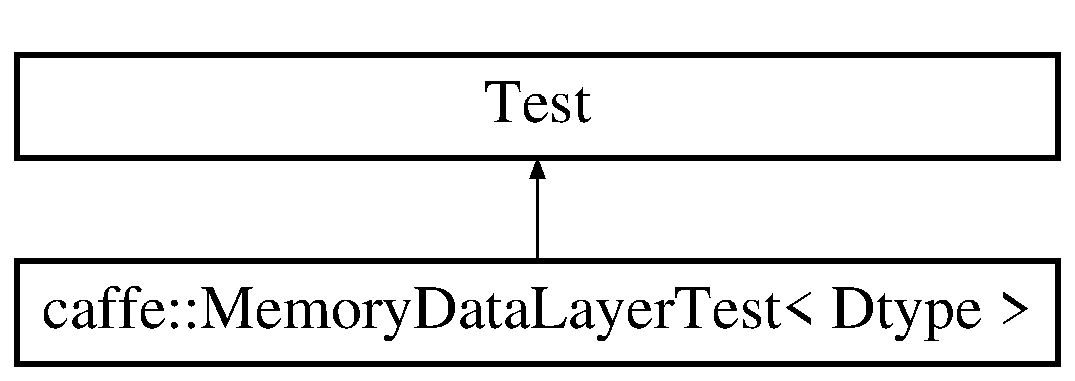
\includegraphics[height=2.000000cm]{classcaffe_1_1_memory_data_layer_test}
\end{center}
\end{figure}
\subsection*{Protected Member Functions}
\begin{DoxyCompactItemize}
\item 
\hyperlink{classcaffe_1_1_memory_data_layer_test_a75d651c270984eb6146e5a00185a86cb}{Memory\+Data\+Layer\+Test} ()
\item 
virtual void \hyperlink{classcaffe_1_1_memory_data_layer_test_a22ac69a349db8a2316ab93baf83763a8}{Set\+Up} ()
\item 
virtual \hyperlink{classcaffe_1_1_memory_data_layer_test_aee42724e86e18c80fd912719e8bc8728}{$\sim$\+Memory\+Data\+Layer\+Test} ()
\end{DoxyCompactItemize}
\subsection*{Protected Attributes}
\begin{DoxyCompactItemize}
\item 
int \hyperlink{classcaffe_1_1_memory_data_layer_test_adf80053b8c93a68ec14207ed114bbf6c}{batch\+\_\+size\+\_\+}
\item 
int \hyperlink{classcaffe_1_1_memory_data_layer_test_ab5cdf08e300fc8ee97762b510403ea1d}{batches\+\_\+}
\item 
int \hyperlink{classcaffe_1_1_memory_data_layer_test_a12cc813a56e6ed0f8f9a341f37adb87b}{channels\+\_\+}
\item 
int \hyperlink{classcaffe_1_1_memory_data_layer_test_ac6f8872f971ff23b79987a812cf6dcac}{height\+\_\+}
\item 
int \hyperlink{classcaffe_1_1_memory_data_layer_test_a3488d10fa611d4deadbf238c288e1572}{width\+\_\+}
\item 
\hyperlink{classcaffe_1_1_blob}{Blob}$<$ Dtype $>$ $\ast$const \hyperlink{classcaffe_1_1_memory_data_layer_test_ad0a921772812e73a2039abb85ffe9968}{data\+\_\+}
\item 
\hyperlink{classcaffe_1_1_blob}{Blob}$<$ Dtype $>$ $\ast$const \hyperlink{classcaffe_1_1_memory_data_layer_test_a2a1b780a38e483da5da7de0852406b0f}{labels\+\_\+}
\item 
\hyperlink{classcaffe_1_1_blob}{Blob}$<$ Dtype $>$ $\ast$const \hyperlink{classcaffe_1_1_memory_data_layer_test_a4b580c8596ec6ce0811a3b785006c9fe}{data\+\_\+blob\+\_\+}
\item 
\hyperlink{classcaffe_1_1_blob}{Blob}$<$ Dtype $>$ $\ast$const \hyperlink{classcaffe_1_1_memory_data_layer_test_a60268033c066e92f4ba6f7b1fa796ab1}{label\+\_\+blob\+\_\+}
\item 
vector$<$ \hyperlink{classcaffe_1_1_blob}{Blob}$<$ Dtype $>$ $\ast$ $>$ \hyperlink{classcaffe_1_1_memory_data_layer_test_abd3b727ea9e820961deab300840f65a8}{blob\+\_\+bottom\+\_\+vec\+\_\+}
\item 
vector$<$ \hyperlink{classcaffe_1_1_blob}{Blob}$<$ Dtype $>$ $\ast$ $>$ \hyperlink{classcaffe_1_1_memory_data_layer_test_ac33a7be28ca9fd66a9981645de4b4423}{blob\+\_\+top\+\_\+vec\+\_\+}
\end{DoxyCompactItemize}


\subsection{Constructor \& Destructor Documentation}
\hypertarget{classcaffe_1_1_memory_data_layer_test_a75d651c270984eb6146e5a00185a86cb}{\index{caffe\+::\+Memory\+Data\+Layer\+Test@{caffe\+::\+Memory\+Data\+Layer\+Test}!Memory\+Data\+Layer\+Test@{Memory\+Data\+Layer\+Test}}
\index{Memory\+Data\+Layer\+Test@{Memory\+Data\+Layer\+Test}!caffe\+::\+Memory\+Data\+Layer\+Test@{caffe\+::\+Memory\+Data\+Layer\+Test}}
\subsubsection[{Memory\+Data\+Layer\+Test}]{\setlength{\rightskip}{0pt plus 5cm}template$<$typename Dtype $>$ {\bf caffe\+::\+Memory\+Data\+Layer\+Test}$<$ Dtype $>$\+::{\bf Memory\+Data\+Layer\+Test} (
\begin{DoxyParamCaption}
{}
\end{DoxyParamCaption}
)\hspace{0.3cm}{\ttfamily [inline]}, {\ttfamily [protected]}}}\label{classcaffe_1_1_memory_data_layer_test_a75d651c270984eb6146e5a00185a86cb}
\hypertarget{classcaffe_1_1_memory_data_layer_test_aee42724e86e18c80fd912719e8bc8728}{\index{caffe\+::\+Memory\+Data\+Layer\+Test@{caffe\+::\+Memory\+Data\+Layer\+Test}!````~Memory\+Data\+Layer\+Test@{$\sim$\+Memory\+Data\+Layer\+Test}}
\index{````~Memory\+Data\+Layer\+Test@{$\sim$\+Memory\+Data\+Layer\+Test}!caffe\+::\+Memory\+Data\+Layer\+Test@{caffe\+::\+Memory\+Data\+Layer\+Test}}
\subsubsection[{$\sim$\+Memory\+Data\+Layer\+Test}]{\setlength{\rightskip}{0pt plus 5cm}template$<$typename Dtype $>$ virtual {\bf caffe\+::\+Memory\+Data\+Layer\+Test}$<$ Dtype $>$\+::$\sim${\bf Memory\+Data\+Layer\+Test} (
\begin{DoxyParamCaption}
{}
\end{DoxyParamCaption}
)\hspace{0.3cm}{\ttfamily [inline]}, {\ttfamily [protected]}, {\ttfamily [virtual]}}}\label{classcaffe_1_1_memory_data_layer_test_aee42724e86e18c80fd912719e8bc8728}


\subsection{Member Function Documentation}
\hypertarget{classcaffe_1_1_memory_data_layer_test_a22ac69a349db8a2316ab93baf83763a8}{\index{caffe\+::\+Memory\+Data\+Layer\+Test@{caffe\+::\+Memory\+Data\+Layer\+Test}!Set\+Up@{Set\+Up}}
\index{Set\+Up@{Set\+Up}!caffe\+::\+Memory\+Data\+Layer\+Test@{caffe\+::\+Memory\+Data\+Layer\+Test}}
\subsubsection[{Set\+Up}]{\setlength{\rightskip}{0pt plus 5cm}template$<$typename Dtype $>$ virtual void {\bf caffe\+::\+Memory\+Data\+Layer\+Test}$<$ Dtype $>$\+::Set\+Up (
\begin{DoxyParamCaption}
{}
\end{DoxyParamCaption}
)\hspace{0.3cm}{\ttfamily [inline]}, {\ttfamily [protected]}, {\ttfamily [virtual]}}}\label{classcaffe_1_1_memory_data_layer_test_a22ac69a349db8a2316ab93baf83763a8}


\subsection{Member Data Documentation}
\hypertarget{classcaffe_1_1_memory_data_layer_test_adf80053b8c93a68ec14207ed114bbf6c}{\index{caffe\+::\+Memory\+Data\+Layer\+Test@{caffe\+::\+Memory\+Data\+Layer\+Test}!batch\+\_\+size\+\_\+@{batch\+\_\+size\+\_\+}}
\index{batch\+\_\+size\+\_\+@{batch\+\_\+size\+\_\+}!caffe\+::\+Memory\+Data\+Layer\+Test@{caffe\+::\+Memory\+Data\+Layer\+Test}}
\subsubsection[{batch\+\_\+size\+\_\+}]{\setlength{\rightskip}{0pt plus 5cm}template$<$typename Dtype $>$ int {\bf caffe\+::\+Memory\+Data\+Layer\+Test}$<$ Dtype $>$\+::batch\+\_\+size\+\_\+\hspace{0.3cm}{\ttfamily [protected]}}}\label{classcaffe_1_1_memory_data_layer_test_adf80053b8c93a68ec14207ed114bbf6c}
\hypertarget{classcaffe_1_1_memory_data_layer_test_ab5cdf08e300fc8ee97762b510403ea1d}{\index{caffe\+::\+Memory\+Data\+Layer\+Test@{caffe\+::\+Memory\+Data\+Layer\+Test}!batches\+\_\+@{batches\+\_\+}}
\index{batches\+\_\+@{batches\+\_\+}!caffe\+::\+Memory\+Data\+Layer\+Test@{caffe\+::\+Memory\+Data\+Layer\+Test}}
\subsubsection[{batches\+\_\+}]{\setlength{\rightskip}{0pt plus 5cm}template$<$typename Dtype $>$ int {\bf caffe\+::\+Memory\+Data\+Layer\+Test}$<$ Dtype $>$\+::batches\+\_\+\hspace{0.3cm}{\ttfamily [protected]}}}\label{classcaffe_1_1_memory_data_layer_test_ab5cdf08e300fc8ee97762b510403ea1d}
\hypertarget{classcaffe_1_1_memory_data_layer_test_abd3b727ea9e820961deab300840f65a8}{\index{caffe\+::\+Memory\+Data\+Layer\+Test@{caffe\+::\+Memory\+Data\+Layer\+Test}!blob\+\_\+bottom\+\_\+vec\+\_\+@{blob\+\_\+bottom\+\_\+vec\+\_\+}}
\index{blob\+\_\+bottom\+\_\+vec\+\_\+@{blob\+\_\+bottom\+\_\+vec\+\_\+}!caffe\+::\+Memory\+Data\+Layer\+Test@{caffe\+::\+Memory\+Data\+Layer\+Test}}
\subsubsection[{blob\+\_\+bottom\+\_\+vec\+\_\+}]{\setlength{\rightskip}{0pt plus 5cm}template$<$typename Dtype $>$ vector$<${\bf Blob}$<$Dtype$>$$\ast$$>$ {\bf caffe\+::\+Memory\+Data\+Layer\+Test}$<$ Dtype $>$\+::blob\+\_\+bottom\+\_\+vec\+\_\+\hspace{0.3cm}{\ttfamily [protected]}}}\label{classcaffe_1_1_memory_data_layer_test_abd3b727ea9e820961deab300840f65a8}
\hypertarget{classcaffe_1_1_memory_data_layer_test_ac33a7be28ca9fd66a9981645de4b4423}{\index{caffe\+::\+Memory\+Data\+Layer\+Test@{caffe\+::\+Memory\+Data\+Layer\+Test}!blob\+\_\+top\+\_\+vec\+\_\+@{blob\+\_\+top\+\_\+vec\+\_\+}}
\index{blob\+\_\+top\+\_\+vec\+\_\+@{blob\+\_\+top\+\_\+vec\+\_\+}!caffe\+::\+Memory\+Data\+Layer\+Test@{caffe\+::\+Memory\+Data\+Layer\+Test}}
\subsubsection[{blob\+\_\+top\+\_\+vec\+\_\+}]{\setlength{\rightskip}{0pt plus 5cm}template$<$typename Dtype $>$ vector$<${\bf Blob}$<$Dtype$>$$\ast$$>$ {\bf caffe\+::\+Memory\+Data\+Layer\+Test}$<$ Dtype $>$\+::blob\+\_\+top\+\_\+vec\+\_\+\hspace{0.3cm}{\ttfamily [protected]}}}\label{classcaffe_1_1_memory_data_layer_test_ac33a7be28ca9fd66a9981645de4b4423}
\hypertarget{classcaffe_1_1_memory_data_layer_test_a12cc813a56e6ed0f8f9a341f37adb87b}{\index{caffe\+::\+Memory\+Data\+Layer\+Test@{caffe\+::\+Memory\+Data\+Layer\+Test}!channels\+\_\+@{channels\+\_\+}}
\index{channels\+\_\+@{channels\+\_\+}!caffe\+::\+Memory\+Data\+Layer\+Test@{caffe\+::\+Memory\+Data\+Layer\+Test}}
\subsubsection[{channels\+\_\+}]{\setlength{\rightskip}{0pt plus 5cm}template$<$typename Dtype $>$ int {\bf caffe\+::\+Memory\+Data\+Layer\+Test}$<$ Dtype $>$\+::channels\+\_\+\hspace{0.3cm}{\ttfamily [protected]}}}\label{classcaffe_1_1_memory_data_layer_test_a12cc813a56e6ed0f8f9a341f37adb87b}
\hypertarget{classcaffe_1_1_memory_data_layer_test_ad0a921772812e73a2039abb85ffe9968}{\index{caffe\+::\+Memory\+Data\+Layer\+Test@{caffe\+::\+Memory\+Data\+Layer\+Test}!data\+\_\+@{data\+\_\+}}
\index{data\+\_\+@{data\+\_\+}!caffe\+::\+Memory\+Data\+Layer\+Test@{caffe\+::\+Memory\+Data\+Layer\+Test}}
\subsubsection[{data\+\_\+}]{\setlength{\rightskip}{0pt plus 5cm}template$<$typename Dtype $>$ {\bf Blob}$<$Dtype$>$$\ast$ const {\bf caffe\+::\+Memory\+Data\+Layer\+Test}$<$ Dtype $>$\+::data\+\_\+\hspace{0.3cm}{\ttfamily [protected]}}}\label{classcaffe_1_1_memory_data_layer_test_ad0a921772812e73a2039abb85ffe9968}
\hypertarget{classcaffe_1_1_memory_data_layer_test_a4b580c8596ec6ce0811a3b785006c9fe}{\index{caffe\+::\+Memory\+Data\+Layer\+Test@{caffe\+::\+Memory\+Data\+Layer\+Test}!data\+\_\+blob\+\_\+@{data\+\_\+blob\+\_\+}}
\index{data\+\_\+blob\+\_\+@{data\+\_\+blob\+\_\+}!caffe\+::\+Memory\+Data\+Layer\+Test@{caffe\+::\+Memory\+Data\+Layer\+Test}}
\subsubsection[{data\+\_\+blob\+\_\+}]{\setlength{\rightskip}{0pt plus 5cm}template$<$typename Dtype $>$ {\bf Blob}$<$Dtype$>$$\ast$ const {\bf caffe\+::\+Memory\+Data\+Layer\+Test}$<$ Dtype $>$\+::data\+\_\+blob\+\_\+\hspace{0.3cm}{\ttfamily [protected]}}}\label{classcaffe_1_1_memory_data_layer_test_a4b580c8596ec6ce0811a3b785006c9fe}
\hypertarget{classcaffe_1_1_memory_data_layer_test_ac6f8872f971ff23b79987a812cf6dcac}{\index{caffe\+::\+Memory\+Data\+Layer\+Test@{caffe\+::\+Memory\+Data\+Layer\+Test}!height\+\_\+@{height\+\_\+}}
\index{height\+\_\+@{height\+\_\+}!caffe\+::\+Memory\+Data\+Layer\+Test@{caffe\+::\+Memory\+Data\+Layer\+Test}}
\subsubsection[{height\+\_\+}]{\setlength{\rightskip}{0pt plus 5cm}template$<$typename Dtype $>$ int {\bf caffe\+::\+Memory\+Data\+Layer\+Test}$<$ Dtype $>$\+::height\+\_\+\hspace{0.3cm}{\ttfamily [protected]}}}\label{classcaffe_1_1_memory_data_layer_test_ac6f8872f971ff23b79987a812cf6dcac}
\hypertarget{classcaffe_1_1_memory_data_layer_test_a60268033c066e92f4ba6f7b1fa796ab1}{\index{caffe\+::\+Memory\+Data\+Layer\+Test@{caffe\+::\+Memory\+Data\+Layer\+Test}!label\+\_\+blob\+\_\+@{label\+\_\+blob\+\_\+}}
\index{label\+\_\+blob\+\_\+@{label\+\_\+blob\+\_\+}!caffe\+::\+Memory\+Data\+Layer\+Test@{caffe\+::\+Memory\+Data\+Layer\+Test}}
\subsubsection[{label\+\_\+blob\+\_\+}]{\setlength{\rightskip}{0pt plus 5cm}template$<$typename Dtype $>$ {\bf Blob}$<$Dtype$>$$\ast$ const {\bf caffe\+::\+Memory\+Data\+Layer\+Test}$<$ Dtype $>$\+::label\+\_\+blob\+\_\+\hspace{0.3cm}{\ttfamily [protected]}}}\label{classcaffe_1_1_memory_data_layer_test_a60268033c066e92f4ba6f7b1fa796ab1}
\hypertarget{classcaffe_1_1_memory_data_layer_test_a2a1b780a38e483da5da7de0852406b0f}{\index{caffe\+::\+Memory\+Data\+Layer\+Test@{caffe\+::\+Memory\+Data\+Layer\+Test}!labels\+\_\+@{labels\+\_\+}}
\index{labels\+\_\+@{labels\+\_\+}!caffe\+::\+Memory\+Data\+Layer\+Test@{caffe\+::\+Memory\+Data\+Layer\+Test}}
\subsubsection[{labels\+\_\+}]{\setlength{\rightskip}{0pt plus 5cm}template$<$typename Dtype $>$ {\bf Blob}$<$Dtype$>$$\ast$ const {\bf caffe\+::\+Memory\+Data\+Layer\+Test}$<$ Dtype $>$\+::labels\+\_\+\hspace{0.3cm}{\ttfamily [protected]}}}\label{classcaffe_1_1_memory_data_layer_test_a2a1b780a38e483da5da7de0852406b0f}
\hypertarget{classcaffe_1_1_memory_data_layer_test_a3488d10fa611d4deadbf238c288e1572}{\index{caffe\+::\+Memory\+Data\+Layer\+Test@{caffe\+::\+Memory\+Data\+Layer\+Test}!width\+\_\+@{width\+\_\+}}
\index{width\+\_\+@{width\+\_\+}!caffe\+::\+Memory\+Data\+Layer\+Test@{caffe\+::\+Memory\+Data\+Layer\+Test}}
\subsubsection[{width\+\_\+}]{\setlength{\rightskip}{0pt plus 5cm}template$<$typename Dtype $>$ int {\bf caffe\+::\+Memory\+Data\+Layer\+Test}$<$ Dtype $>$\+::width\+\_\+\hspace{0.3cm}{\ttfamily [protected]}}}\label{classcaffe_1_1_memory_data_layer_test_a3488d10fa611d4deadbf238c288e1572}


The documentation for this class was generated from the following file\+:\begin{DoxyCompactItemize}
\item 
src/caffe/test/\hyperlink{test__memory__data__layer_8cpp}{test\+\_\+memory\+\_\+data\+\_\+layer.\+cpp}\end{DoxyCompactItemize}

\hypertarget{classcaffe_1_1_multinomial_logistic_loss_layer}{\section{caffe\+:\+:Multinomial\+Logistic\+Loss\+Layer$<$ Dtype $>$ Class Template Reference}
\label{classcaffe_1_1_multinomial_logistic_loss_layer}\index{caffe\+::\+Multinomial\+Logistic\+Loss\+Layer$<$ Dtype $>$@{caffe\+::\+Multinomial\+Logistic\+Loss\+Layer$<$ Dtype $>$}}
}


{\ttfamily \#include $<$vision\+\_\+layers.\+hpp$>$}

Inheritance diagram for caffe\+:\+:Multinomial\+Logistic\+Loss\+Layer$<$ Dtype $>$\+:\begin{figure}[H]
\begin{center}
\leavevmode
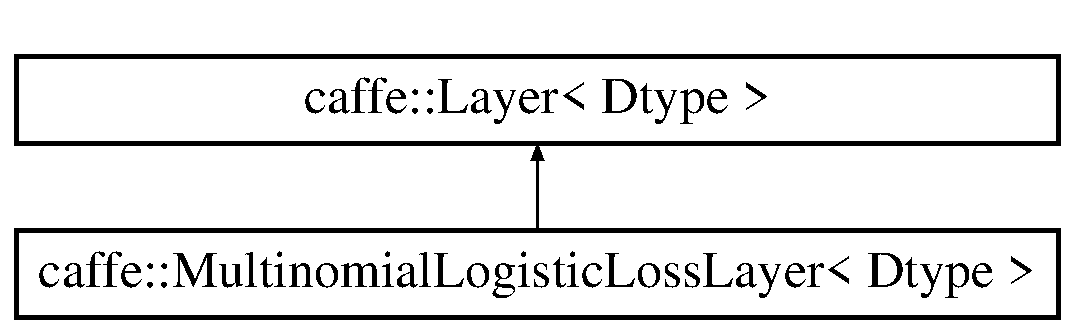
\includegraphics[height=2.000000cm]{classcaffe_1_1_multinomial_logistic_loss_layer}
\end{center}
\end{figure}
\subsection*{Public Member Functions}
\begin{DoxyCompactItemize}
\item 
\hyperlink{classcaffe_1_1_multinomial_logistic_loss_layer_a1c9567f9901885ec4737cf9315d52081}{Multinomial\+Logistic\+Loss\+Layer} (const Layer\+Parameter \&param)
\item 
virtual void \hyperlink{classcaffe_1_1_multinomial_logistic_loss_layer_af706bf27c3170a243660e7fe46ad0686}{Set\+Up} (const vector$<$ \hyperlink{classcaffe_1_1_blob}{Blob}$<$ Dtype $>$ $\ast$ $>$ \&bottom, vector$<$ \hyperlink{classcaffe_1_1_blob}{Blob}$<$ Dtype $>$ $\ast$ $>$ $\ast$top)
\end{DoxyCompactItemize}
\subsection*{Protected Member Functions}
\begin{DoxyCompactItemize}
\item 
virtual Dtype \hyperlink{classcaffe_1_1_multinomial_logistic_loss_layer_a5c506ead552d2764df152dd9c90b768b}{Forward\+\_\+cpu} (const vector$<$ \hyperlink{classcaffe_1_1_blob}{Blob}$<$ Dtype $>$ $\ast$ $>$ \&bottom, vector$<$ \hyperlink{classcaffe_1_1_blob}{Blob}$<$ Dtype $>$ $\ast$ $>$ $\ast$top)
\item 
virtual void \hyperlink{classcaffe_1_1_multinomial_logistic_loss_layer_a130cef8084d30fc789c401ec0310d587}{Backward\+\_\+cpu} (const vector$<$ \hyperlink{classcaffe_1_1_blob}{Blob}$<$ Dtype $>$ $\ast$ $>$ \&top, const bool propagate\+\_\+down, vector$<$ \hyperlink{classcaffe_1_1_blob}{Blob}$<$ Dtype $>$ $\ast$ $>$ $\ast$bottom)
\end{DoxyCompactItemize}
\subsection*{Additional Inherited Members}


\subsection{Constructor \& Destructor Documentation}
\hypertarget{classcaffe_1_1_multinomial_logistic_loss_layer_a1c9567f9901885ec4737cf9315d52081}{\index{caffe\+::\+Multinomial\+Logistic\+Loss\+Layer@{caffe\+::\+Multinomial\+Logistic\+Loss\+Layer}!Multinomial\+Logistic\+Loss\+Layer@{Multinomial\+Logistic\+Loss\+Layer}}
\index{Multinomial\+Logistic\+Loss\+Layer@{Multinomial\+Logistic\+Loss\+Layer}!caffe\+::\+Multinomial\+Logistic\+Loss\+Layer@{caffe\+::\+Multinomial\+Logistic\+Loss\+Layer}}
\subsubsection[{Multinomial\+Logistic\+Loss\+Layer}]{\setlength{\rightskip}{0pt plus 5cm}template$<$typename Dtype $>$ {\bf caffe\+::\+Multinomial\+Logistic\+Loss\+Layer}$<$ Dtype $>$\+::{\bf Multinomial\+Logistic\+Loss\+Layer} (
\begin{DoxyParamCaption}
\item[{const Layer\+Parameter \&}]{param}
\end{DoxyParamCaption}
)\hspace{0.3cm}{\ttfamily [inline]}, {\ttfamily [explicit]}}}\label{classcaffe_1_1_multinomial_logistic_loss_layer_a1c9567f9901885ec4737cf9315d52081}


\subsection{Member Function Documentation}
\hypertarget{classcaffe_1_1_multinomial_logistic_loss_layer_a130cef8084d30fc789c401ec0310d587}{\index{caffe\+::\+Multinomial\+Logistic\+Loss\+Layer@{caffe\+::\+Multinomial\+Logistic\+Loss\+Layer}!Backward\+\_\+cpu@{Backward\+\_\+cpu}}
\index{Backward\+\_\+cpu@{Backward\+\_\+cpu}!caffe\+::\+Multinomial\+Logistic\+Loss\+Layer@{caffe\+::\+Multinomial\+Logistic\+Loss\+Layer}}
\subsubsection[{Backward\+\_\+cpu}]{\setlength{\rightskip}{0pt plus 5cm}template$<$typename Dtype $>$ void {\bf caffe\+::\+Multinomial\+Logistic\+Loss\+Layer}$<$ Dtype $>$\+::Backward\+\_\+cpu (
\begin{DoxyParamCaption}
\item[{const vector$<$ {\bf Blob}$<$ Dtype $>$ $\ast$ $>$ \&}]{top, }
\item[{const bool}]{propagate\+\_\+down, }
\item[{vector$<$ {\bf Blob}$<$ Dtype $>$ $\ast$ $>$ $\ast$}]{bottom}
\end{DoxyParamCaption}
)\hspace{0.3cm}{\ttfamily [protected]}, {\ttfamily [virtual]}}}\label{classcaffe_1_1_multinomial_logistic_loss_layer_a130cef8084d30fc789c401ec0310d587}


Implements \hyperlink{classcaffe_1_1_layer_ac2d82011d076237c67997f63e7ee4b80}{caffe\+::\+Layer$<$ Dtype $>$}.

\hypertarget{classcaffe_1_1_multinomial_logistic_loss_layer_a5c506ead552d2764df152dd9c90b768b}{\index{caffe\+::\+Multinomial\+Logistic\+Loss\+Layer@{caffe\+::\+Multinomial\+Logistic\+Loss\+Layer}!Forward\+\_\+cpu@{Forward\+\_\+cpu}}
\index{Forward\+\_\+cpu@{Forward\+\_\+cpu}!caffe\+::\+Multinomial\+Logistic\+Loss\+Layer@{caffe\+::\+Multinomial\+Logistic\+Loss\+Layer}}
\subsubsection[{Forward\+\_\+cpu}]{\setlength{\rightskip}{0pt plus 5cm}template$<$typename Dtype $>$ Dtype {\bf caffe\+::\+Multinomial\+Logistic\+Loss\+Layer}$<$ Dtype $>$\+::Forward\+\_\+cpu (
\begin{DoxyParamCaption}
\item[{const vector$<$ {\bf Blob}$<$ Dtype $>$ $\ast$ $>$ \&}]{bottom, }
\item[{vector$<$ {\bf Blob}$<$ Dtype $>$ $\ast$ $>$ $\ast$}]{top}
\end{DoxyParamCaption}
)\hspace{0.3cm}{\ttfamily [protected]}, {\ttfamily [virtual]}}}\label{classcaffe_1_1_multinomial_logistic_loss_layer_a5c506ead552d2764df152dd9c90b768b}


Implements \hyperlink{classcaffe_1_1_layer_a8f7f61da3b8b3ca7f2394dee33873353}{caffe\+::\+Layer$<$ Dtype $>$}.

\hypertarget{classcaffe_1_1_multinomial_logistic_loss_layer_af706bf27c3170a243660e7fe46ad0686}{\index{caffe\+::\+Multinomial\+Logistic\+Loss\+Layer@{caffe\+::\+Multinomial\+Logistic\+Loss\+Layer}!Set\+Up@{Set\+Up}}
\index{Set\+Up@{Set\+Up}!caffe\+::\+Multinomial\+Logistic\+Loss\+Layer@{caffe\+::\+Multinomial\+Logistic\+Loss\+Layer}}
\subsubsection[{Set\+Up}]{\setlength{\rightskip}{0pt plus 5cm}template$<$typename Dtype $>$ void {\bf caffe\+::\+Multinomial\+Logistic\+Loss\+Layer}$<$ Dtype $>$\+::Set\+Up (
\begin{DoxyParamCaption}
\item[{const vector$<$ {\bf Blob}$<$ Dtype $>$ $\ast$ $>$ \&}]{bottom, }
\item[{vector$<$ {\bf Blob}$<$ Dtype $>$ $\ast$ $>$ $\ast$}]{top}
\end{DoxyParamCaption}
)\hspace{0.3cm}{\ttfamily [virtual]}}}\label{classcaffe_1_1_multinomial_logistic_loss_layer_af706bf27c3170a243660e7fe46ad0686}


Implements \hyperlink{classcaffe_1_1_layer_abd13c6489c13953b4fbcfcf6880835d0}{caffe\+::\+Layer$<$ Dtype $>$}.



The documentation for this class was generated from the following files\+:\begin{DoxyCompactItemize}
\item 
include/caffe/\hyperlink{vision__layers_8hpp}{vision\+\_\+layers.\+hpp}\item 
src/caffe/layers/\hyperlink{loss__layer_8cpp}{loss\+\_\+layer.\+cpp}\end{DoxyCompactItemize}

\hypertarget{classcaffe_1_1_multinomial_logistic_loss_layer_test}{\section{caffe\+:\+:Multinomial\+Logistic\+Loss\+Layer\+Test$<$ Dtype $>$ Class Template Reference}
\label{classcaffe_1_1_multinomial_logistic_loss_layer_test}\index{caffe\+::\+Multinomial\+Logistic\+Loss\+Layer\+Test$<$ Dtype $>$@{caffe\+::\+Multinomial\+Logistic\+Loss\+Layer\+Test$<$ Dtype $>$}}
}
Inheritance diagram for caffe\+:\+:Multinomial\+Logistic\+Loss\+Layer\+Test$<$ Dtype $>$\+:\begin{figure}[H]
\begin{center}
\leavevmode
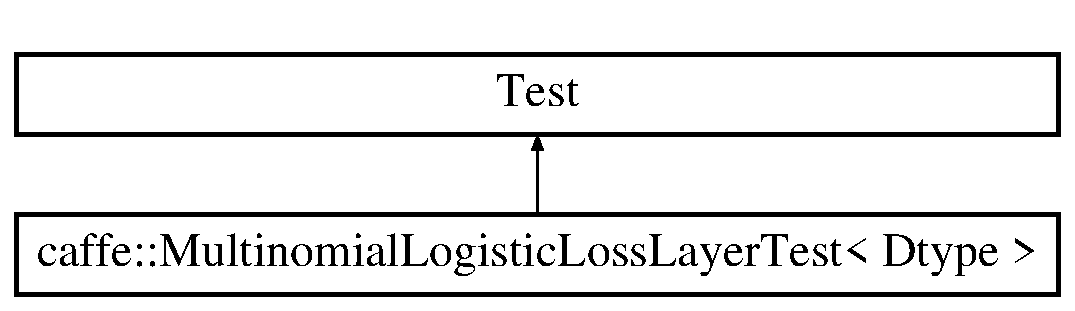
\includegraphics[height=2.000000cm]{classcaffe_1_1_multinomial_logistic_loss_layer_test}
\end{center}
\end{figure}
\subsection*{Protected Member Functions}
\begin{DoxyCompactItemize}
\item 
\hyperlink{classcaffe_1_1_multinomial_logistic_loss_layer_test_a098d2b1a8732f778882526813d55e658}{Multinomial\+Logistic\+Loss\+Layer\+Test} ()
\item 
virtual \hyperlink{classcaffe_1_1_multinomial_logistic_loss_layer_test_ab8c2c439b175da09d87e5bfcf4f87779}{$\sim$\+Multinomial\+Logistic\+Loss\+Layer\+Test} ()
\end{DoxyCompactItemize}
\subsection*{Protected Attributes}
\begin{DoxyCompactItemize}
\item 
\hyperlink{classcaffe_1_1_blob}{Blob}$<$ Dtype $>$ $\ast$const \hyperlink{classcaffe_1_1_multinomial_logistic_loss_layer_test_a3ff6abb2618f4ea1257e3f423e2d1bef}{blob\+\_\+bottom\+\_\+data\+\_\+}
\item 
\hyperlink{classcaffe_1_1_blob}{Blob}$<$ Dtype $>$ $\ast$const \hyperlink{classcaffe_1_1_multinomial_logistic_loss_layer_test_a8d187356bce9457509a461e4aad1ea0b}{blob\+\_\+bottom\+\_\+label\+\_\+}
\item 
vector$<$ \hyperlink{classcaffe_1_1_blob}{Blob}$<$ Dtype $>$ $\ast$ $>$ \hyperlink{classcaffe_1_1_multinomial_logistic_loss_layer_test_a1e54a2b39c6607f7addf35509af7ff1f}{blob\+\_\+bottom\+\_\+vec\+\_\+}
\item 
vector$<$ \hyperlink{classcaffe_1_1_blob}{Blob}$<$ Dtype $>$ $\ast$ $>$ \hyperlink{classcaffe_1_1_multinomial_logistic_loss_layer_test_a4783a4aa643582e0d8ee36eb9fc44889}{blob\+\_\+top\+\_\+vec\+\_\+}
\end{DoxyCompactItemize}


\subsection{Constructor \& Destructor Documentation}
\hypertarget{classcaffe_1_1_multinomial_logistic_loss_layer_test_a098d2b1a8732f778882526813d55e658}{\index{caffe\+::\+Multinomial\+Logistic\+Loss\+Layer\+Test@{caffe\+::\+Multinomial\+Logistic\+Loss\+Layer\+Test}!Multinomial\+Logistic\+Loss\+Layer\+Test@{Multinomial\+Logistic\+Loss\+Layer\+Test}}
\index{Multinomial\+Logistic\+Loss\+Layer\+Test@{Multinomial\+Logistic\+Loss\+Layer\+Test}!caffe\+::\+Multinomial\+Logistic\+Loss\+Layer\+Test@{caffe\+::\+Multinomial\+Logistic\+Loss\+Layer\+Test}}
\subsubsection[{Multinomial\+Logistic\+Loss\+Layer\+Test}]{\setlength{\rightskip}{0pt plus 5cm}template$<$typename Dtype $>$ {\bf caffe\+::\+Multinomial\+Logistic\+Loss\+Layer\+Test}$<$ Dtype $>$\+::{\bf Multinomial\+Logistic\+Loss\+Layer\+Test} (
\begin{DoxyParamCaption}
{}
\end{DoxyParamCaption}
)\hspace{0.3cm}{\ttfamily [inline]}, {\ttfamily [protected]}}}\label{classcaffe_1_1_multinomial_logistic_loss_layer_test_a098d2b1a8732f778882526813d55e658}
\hypertarget{classcaffe_1_1_multinomial_logistic_loss_layer_test_ab8c2c439b175da09d87e5bfcf4f87779}{\index{caffe\+::\+Multinomial\+Logistic\+Loss\+Layer\+Test@{caffe\+::\+Multinomial\+Logistic\+Loss\+Layer\+Test}!````~Multinomial\+Logistic\+Loss\+Layer\+Test@{$\sim$\+Multinomial\+Logistic\+Loss\+Layer\+Test}}
\index{````~Multinomial\+Logistic\+Loss\+Layer\+Test@{$\sim$\+Multinomial\+Logistic\+Loss\+Layer\+Test}!caffe\+::\+Multinomial\+Logistic\+Loss\+Layer\+Test@{caffe\+::\+Multinomial\+Logistic\+Loss\+Layer\+Test}}
\subsubsection[{$\sim$\+Multinomial\+Logistic\+Loss\+Layer\+Test}]{\setlength{\rightskip}{0pt plus 5cm}template$<$typename Dtype $>$ virtual {\bf caffe\+::\+Multinomial\+Logistic\+Loss\+Layer\+Test}$<$ Dtype $>$\+::$\sim${\bf Multinomial\+Logistic\+Loss\+Layer\+Test} (
\begin{DoxyParamCaption}
{}
\end{DoxyParamCaption}
)\hspace{0.3cm}{\ttfamily [inline]}, {\ttfamily [protected]}, {\ttfamily [virtual]}}}\label{classcaffe_1_1_multinomial_logistic_loss_layer_test_ab8c2c439b175da09d87e5bfcf4f87779}


\subsection{Member Data Documentation}
\hypertarget{classcaffe_1_1_multinomial_logistic_loss_layer_test_a3ff6abb2618f4ea1257e3f423e2d1bef}{\index{caffe\+::\+Multinomial\+Logistic\+Loss\+Layer\+Test@{caffe\+::\+Multinomial\+Logistic\+Loss\+Layer\+Test}!blob\+\_\+bottom\+\_\+data\+\_\+@{blob\+\_\+bottom\+\_\+data\+\_\+}}
\index{blob\+\_\+bottom\+\_\+data\+\_\+@{blob\+\_\+bottom\+\_\+data\+\_\+}!caffe\+::\+Multinomial\+Logistic\+Loss\+Layer\+Test@{caffe\+::\+Multinomial\+Logistic\+Loss\+Layer\+Test}}
\subsubsection[{blob\+\_\+bottom\+\_\+data\+\_\+}]{\setlength{\rightskip}{0pt plus 5cm}template$<$typename Dtype $>$ {\bf Blob}$<$Dtype$>$$\ast$ const {\bf caffe\+::\+Multinomial\+Logistic\+Loss\+Layer\+Test}$<$ Dtype $>$\+::blob\+\_\+bottom\+\_\+data\+\_\+\hspace{0.3cm}{\ttfamily [protected]}}}\label{classcaffe_1_1_multinomial_logistic_loss_layer_test_a3ff6abb2618f4ea1257e3f423e2d1bef}
\hypertarget{classcaffe_1_1_multinomial_logistic_loss_layer_test_a8d187356bce9457509a461e4aad1ea0b}{\index{caffe\+::\+Multinomial\+Logistic\+Loss\+Layer\+Test@{caffe\+::\+Multinomial\+Logistic\+Loss\+Layer\+Test}!blob\+\_\+bottom\+\_\+label\+\_\+@{blob\+\_\+bottom\+\_\+label\+\_\+}}
\index{blob\+\_\+bottom\+\_\+label\+\_\+@{blob\+\_\+bottom\+\_\+label\+\_\+}!caffe\+::\+Multinomial\+Logistic\+Loss\+Layer\+Test@{caffe\+::\+Multinomial\+Logistic\+Loss\+Layer\+Test}}
\subsubsection[{blob\+\_\+bottom\+\_\+label\+\_\+}]{\setlength{\rightskip}{0pt plus 5cm}template$<$typename Dtype $>$ {\bf Blob}$<$Dtype$>$$\ast$ const {\bf caffe\+::\+Multinomial\+Logistic\+Loss\+Layer\+Test}$<$ Dtype $>$\+::blob\+\_\+bottom\+\_\+label\+\_\+\hspace{0.3cm}{\ttfamily [protected]}}}\label{classcaffe_1_1_multinomial_logistic_loss_layer_test_a8d187356bce9457509a461e4aad1ea0b}
\hypertarget{classcaffe_1_1_multinomial_logistic_loss_layer_test_a1e54a2b39c6607f7addf35509af7ff1f}{\index{caffe\+::\+Multinomial\+Logistic\+Loss\+Layer\+Test@{caffe\+::\+Multinomial\+Logistic\+Loss\+Layer\+Test}!blob\+\_\+bottom\+\_\+vec\+\_\+@{blob\+\_\+bottom\+\_\+vec\+\_\+}}
\index{blob\+\_\+bottom\+\_\+vec\+\_\+@{blob\+\_\+bottom\+\_\+vec\+\_\+}!caffe\+::\+Multinomial\+Logistic\+Loss\+Layer\+Test@{caffe\+::\+Multinomial\+Logistic\+Loss\+Layer\+Test}}
\subsubsection[{blob\+\_\+bottom\+\_\+vec\+\_\+}]{\setlength{\rightskip}{0pt plus 5cm}template$<$typename Dtype $>$ vector$<${\bf Blob}$<$Dtype$>$$\ast$$>$ {\bf caffe\+::\+Multinomial\+Logistic\+Loss\+Layer\+Test}$<$ Dtype $>$\+::blob\+\_\+bottom\+\_\+vec\+\_\+\hspace{0.3cm}{\ttfamily [protected]}}}\label{classcaffe_1_1_multinomial_logistic_loss_layer_test_a1e54a2b39c6607f7addf35509af7ff1f}
\hypertarget{classcaffe_1_1_multinomial_logistic_loss_layer_test_a4783a4aa643582e0d8ee36eb9fc44889}{\index{caffe\+::\+Multinomial\+Logistic\+Loss\+Layer\+Test@{caffe\+::\+Multinomial\+Logistic\+Loss\+Layer\+Test}!blob\+\_\+top\+\_\+vec\+\_\+@{blob\+\_\+top\+\_\+vec\+\_\+}}
\index{blob\+\_\+top\+\_\+vec\+\_\+@{blob\+\_\+top\+\_\+vec\+\_\+}!caffe\+::\+Multinomial\+Logistic\+Loss\+Layer\+Test@{caffe\+::\+Multinomial\+Logistic\+Loss\+Layer\+Test}}
\subsubsection[{blob\+\_\+top\+\_\+vec\+\_\+}]{\setlength{\rightskip}{0pt plus 5cm}template$<$typename Dtype $>$ vector$<${\bf Blob}$<$Dtype$>$$\ast$$>$ {\bf caffe\+::\+Multinomial\+Logistic\+Loss\+Layer\+Test}$<$ Dtype $>$\+::blob\+\_\+top\+\_\+vec\+\_\+\hspace{0.3cm}{\ttfamily [protected]}}}\label{classcaffe_1_1_multinomial_logistic_loss_layer_test_a4783a4aa643582e0d8ee36eb9fc44889}


The documentation for this class was generated from the following file\+:\begin{DoxyCompactItemize}
\item 
src/caffe/test/\hyperlink{test__multinomial__logistic__loss__layer_8cpp}{test\+\_\+multinomial\+\_\+logistic\+\_\+loss\+\_\+layer.\+cpp}\end{DoxyCompactItemize}

\hypertarget{classcaffe_1_1_net}{\section{caffe\+:\+:Net$<$ Dtype $>$ Class Template Reference}
\label{classcaffe_1_1_net}\index{caffe\+::\+Net$<$ Dtype $>$@{caffe\+::\+Net$<$ Dtype $>$}}
}


{\ttfamily \#include $<$net.\+hpp$>$}

\subsection*{Public Member Functions}
\begin{DoxyCompactItemize}
\item 
\hyperlink{classcaffe_1_1_net_a5a5655a49c702c6c4a2f5bd7bf7adf12}{Net} (const Net\+Parameter \&param)
\item 
\hyperlink{classcaffe_1_1_net_adda8f582b67677815d77dfc14946772b}{Net} (const string \&param\+\_\+file)
\item 
virtual \hyperlink{classcaffe_1_1_net_adb39f6b979f88d3408992d29d70d3454}{$\sim$\+Net} ()
\item 
void \hyperlink{classcaffe_1_1_net_ae9fcfaabc89165d6c0cb4b14b4c6b584}{Init} (const Net\+Parameter \&param)
\item 
const vector$<$ \hyperlink{classcaffe_1_1_blob}{Blob}$<$ Dtype $>$ $\ast$ $>$ \& \hyperlink{classcaffe_1_1_net_a7e2fd4143799072b500bc8ced53353cd}{Forward\+Prefilled} (Dtype $\ast$loss=N\+U\+L\+L)
\item 
const vector$<$ \hyperlink{classcaffe_1_1_blob}{Blob}$<$ Dtype $>$ $\ast$ $>$ \& \hyperlink{classcaffe_1_1_net_ad12d1ab8e1beb2e407e82454b174f83a}{Forward} (const vector$<$ \hyperlink{classcaffe_1_1_blob}{Blob}$<$ Dtype $>$ $\ast$ $>$ \&bottom, Dtype $\ast$loss=N\+U\+L\+L)
\item 
string \hyperlink{classcaffe_1_1_net_ad97c5e2984017e0a893a5c396fc8beb8}{Forward} (const string \&input\+\_\+blob\+\_\+protos, Dtype $\ast$loss=N\+U\+L\+L)
\item 
void \hyperlink{classcaffe_1_1_net_a7a1a6d17347106dd1284b1b6d28cb4e9}{Backward} ()
\item 
Dtype \hyperlink{classcaffe_1_1_net_ac735151133dcdc9e4ece8eca6c8c3835}{Forward\+Backward} (const vector$<$ \hyperlink{classcaffe_1_1_blob}{Blob}$<$ Dtype $>$ $\ast$ $>$ \&bottom)
\item 
void \hyperlink{classcaffe_1_1_net_a8a2544cefc59d6cbe1bf634f5d5be1c5}{Update} ()
\item 
void \hyperlink{classcaffe_1_1_net_a01d1c1505ff1360de6aa14fa117279cc}{Share\+Trained\+Layers\+With} (\hyperlink{classcaffe_1_1_net}{Net} $\ast$other)
\item 
void \hyperlink{classcaffe_1_1_net_a4ac2b69748470f54d530bc5dfa05b9c3}{Copy\+Trained\+Layers\+From} (const Net\+Parameter \&param)
\item 
void \hyperlink{classcaffe_1_1_net_ad5e222ad89011558cee681133e5c610b}{Copy\+Trained\+Layers\+From} (const string trained\+\_\+filename)
\item 
void \hyperlink{classcaffe_1_1_net_a81de7f48c2ecb431496b2e70754e74fd}{To\+Proto} (Net\+Parameter $\ast$param, bool write\+\_\+diff=false)
\item 
const string \& \hyperlink{classcaffe_1_1_net_a101a9872250ffac595edb163b0c88e96}{name} ()
\item 
const vector$<$ string $>$ \& \hyperlink{classcaffe_1_1_net_a2daa2a72fe29bf58f14d8c7ab943ea9b}{layer\+\_\+names} ()
\item 
const vector$<$ string $>$ \& \hyperlink{classcaffe_1_1_net_a0a8dd2d0630a7fb5b35beb217ffd857a}{blob\+\_\+names} ()
\item 
const vector$<$ shared\+\_\+ptr$<$ \hyperlink{classcaffe_1_1_blob}{Blob}\\*
$<$ Dtype $>$ $>$ $>$ \& \hyperlink{classcaffe_1_1_net_a5fe377d90f21430b028c7cef1cd6ac2d}{blobs} ()
\item 
const vector$<$ shared\+\_\+ptr\\*
$<$ \hyperlink{classcaffe_1_1_layer}{Layer}$<$ Dtype $>$ $>$ $>$ \& \hyperlink{classcaffe_1_1_net_aa5185fed7df3fdd05e289459340571b3}{layers} ()
\item 
vector$<$ vector$<$ \hyperlink{classcaffe_1_1_blob}{Blob}$<$ Dtype $>$ $\ast$ $>$ $>$ \& \hyperlink{classcaffe_1_1_net_aa4e28420adc6c5c19e23ee1e3b131cca}{bottom\+\_\+vecs} ()
\item 
vector$<$ vector$<$ \hyperlink{classcaffe_1_1_blob}{Blob}$<$ Dtype $>$ $\ast$ $>$ $>$ \& \hyperlink{classcaffe_1_1_net_a4d145523a8596627f740b9adfd5ebef5}{top\+\_\+vecs} ()
\item 
vector$<$ shared\+\_\+ptr$<$ \hyperlink{classcaffe_1_1_blob}{Blob}\\*
$<$ Dtype $>$ $>$ $>$ \& \hyperlink{classcaffe_1_1_net_a59dccb44a585213886c0748bebc52303}{params} ()
\item 
vector$<$ float $>$ \& \hyperlink{classcaffe_1_1_net_a34018b12a617b908086ba869d05a2c7c}{params\+\_\+lr} ()
\item 
vector$<$ float $>$ \& \hyperlink{classcaffe_1_1_net_a2eafb0098fee6f41d70a6a7e8feef650}{params\+\_\+weight\+\_\+decay} ()
\item 
int \hyperlink{classcaffe_1_1_net_a5e9d22ba3d645b3fcd806e6d4ac84407}{num\+\_\+inputs} ()
\item 
int \hyperlink{classcaffe_1_1_net_ac584f6ccbefdc6d9e5a498e06dcfb9d6}{num\+\_\+outputs} ()
\item 
vector$<$ \hyperlink{classcaffe_1_1_blob}{Blob}$<$ Dtype $>$ $\ast$ $>$ \& \hyperlink{classcaffe_1_1_net_a1ef3770e0fec193f6ee14ca1a7eb7c9a}{input\+\_\+blobs} ()
\item 
vector$<$ \hyperlink{classcaffe_1_1_blob}{Blob}$<$ Dtype $>$ $\ast$ $>$ \& \hyperlink{classcaffe_1_1_net_ac9d72d39f7d4b8d68c6d400f60eefb39}{output\+\_\+blobs} ()
\item 
bool \hyperlink{classcaffe_1_1_net_a860b9340527c9b41c9744ec71c705682}{has\+\_\+blob} (const string \&blob\+\_\+name)
\item 
const shared\+\_\+ptr$<$ \hyperlink{classcaffe_1_1_blob}{Blob}$<$ Dtype $>$ $>$ \hyperlink{classcaffe_1_1_net_a032a2be8752ae4d4123677afbcebc744}{blob\+\_\+by\+\_\+name} (const string \&blob\+\_\+name)
\item 
bool \hyperlink{classcaffe_1_1_net_a93f62dd95e25cbbac68dc686d9366dc8}{has\+\_\+layer} (const string \&layer\+\_\+name)
\item 
const shared\+\_\+ptr$<$ \hyperlink{classcaffe_1_1_layer}{Layer}$<$ Dtype $>$ $>$ \hyperlink{classcaffe_1_1_net_aafb72f05150abc94af5317d1b33b197b}{layer\+\_\+by\+\_\+name} (const string \&layer\+\_\+name)
\end{DoxyCompactItemize}
\subsection*{Protected Member Functions}
\begin{DoxyCompactItemize}
\item 
void \hyperlink{classcaffe_1_1_net_a9b298f9b34469e0ec2bd1b58df84b128}{Get\+Learning\+Rate\+And\+Weight\+Decay} ()
\item 
\hyperlink{classcaffe_1_1_net_a3d52b2d075fa543e687cf61ba035a488}{D\+I\+S\+A\+B\+L\+E\+\_\+\+C\+O\+P\+Y\+\_\+\+A\+N\+D\+\_\+\+A\+S\+S\+I\+G\+N} (\hyperlink{classcaffe_1_1_net}{Net})
\end{DoxyCompactItemize}
\subsection*{Protected Attributes}
\begin{DoxyCompactItemize}
\item 
vector$<$ shared\+\_\+ptr$<$ \hyperlink{classcaffe_1_1_layer}{Layer}\\*
$<$ Dtype $>$ $>$ $>$ \hyperlink{classcaffe_1_1_net_ab9e30392aa01dcf182d1a5cbd34ec45e}{layers\+\_\+}
\item 
vector$<$ string $>$ \hyperlink{classcaffe_1_1_net_ac792353f3cac826d97feea4b9eff3dff}{layer\+\_\+names\+\_\+}
\item 
map$<$ string, int $>$ \hyperlink{classcaffe_1_1_net_a41db3e5f1fd7a28c58a2c605a6af0c3b}{layer\+\_\+names\+\_\+index\+\_\+}
\item 
vector$<$ bool $>$ \hyperlink{classcaffe_1_1_net_a4c4dbb09376c663637e2444a4fd452b0}{layer\+\_\+need\+\_\+backward\+\_\+}
\item 
vector$<$ shared\+\_\+ptr$<$ \hyperlink{classcaffe_1_1_blob}{Blob}\\*
$<$ Dtype $>$ $>$ $>$ \hyperlink{classcaffe_1_1_net_ab033c0574fcbf1e67e22b9682677c64d}{blobs\+\_\+}
\item 
vector$<$ string $>$ \hyperlink{classcaffe_1_1_net_a0055d38b35ea1a2f44bd400dd6d10846}{blob\+\_\+names\+\_\+}
\item 
map$<$ string, int $>$ \hyperlink{classcaffe_1_1_net_a45f232e36045689438a7e1d869ed399c}{blob\+\_\+names\+\_\+index\+\_\+}
\item 
vector$<$ bool $>$ \hyperlink{classcaffe_1_1_net_a16cedebd7cc82e0b3a30617b71d4c3f7}{blob\+\_\+need\+\_\+backward\+\_\+}
\item 
vector$<$ vector$<$ \hyperlink{classcaffe_1_1_blob}{Blob}$<$ Dtype $>$ $\ast$ $>$ $>$ \hyperlink{classcaffe_1_1_net_ac5bf2007047f749d9d111b0dfa220afc}{bottom\+\_\+vecs\+\_\+}
\item 
vector$<$ vector$<$ int $>$ $>$ \hyperlink{classcaffe_1_1_net_a49ce49e288297963f0d9f7a6d790daa6}{bottom\+\_\+id\+\_\+vecs\+\_\+}
\item 
vector$<$ vector$<$ \hyperlink{classcaffe_1_1_blob}{Blob}$<$ Dtype $>$ $\ast$ $>$ $>$ \hyperlink{classcaffe_1_1_net_aa834096a02382d9a881bf33694e72564}{top\+\_\+vecs\+\_\+}
\item 
vector$<$ vector$<$ int $>$ $>$ \hyperlink{classcaffe_1_1_net_aacacd1d6a07c61694433d4ce5ca8b0be}{top\+\_\+id\+\_\+vecs\+\_\+}
\item 
vector$<$ int $>$ \hyperlink{classcaffe_1_1_net_a083a9a4c3919721c833b53d5571a7400}{net\+\_\+input\+\_\+blob\+\_\+indices\+\_\+}
\item 
vector$<$ \hyperlink{classcaffe_1_1_blob}{Blob}$<$ Dtype $>$ $\ast$ $>$ \hyperlink{classcaffe_1_1_net_aeed682088cd2252f8402cb7b169d4f39}{net\+\_\+input\+\_\+blobs\+\_\+}
\item 
vector$<$ \hyperlink{classcaffe_1_1_blob}{Blob}$<$ Dtype $>$ $\ast$ $>$ \hyperlink{classcaffe_1_1_net_abbcd68a31a7ddc67dcac789fe880da23}{net\+\_\+output\+\_\+blobs\+\_\+}
\item 
string \hyperlink{classcaffe_1_1_net_aef7021f31e355ab8f8991755125f6b2b}{name\+\_\+}
\item 
vector$<$ shared\+\_\+ptr$<$ \hyperlink{classcaffe_1_1_blob}{Blob}\\*
$<$ Dtype $>$ $>$ $>$ \hyperlink{classcaffe_1_1_net_accf52332675952dd27dfc8d3c27fa583}{params\+\_\+}
\item 
vector$<$ float $>$ \hyperlink{classcaffe_1_1_net_aeb1f85c97372f57336e4e1af3eb7b9db}{params\+\_\+lr\+\_\+}
\item 
vector$<$ float $>$ \hyperlink{classcaffe_1_1_net_ad337cf5b16e69533f605dbe1f6932bc9}{params\+\_\+weight\+\_\+decay\+\_\+}
\end{DoxyCompactItemize}


\subsection{Constructor \& Destructor Documentation}
\hypertarget{classcaffe_1_1_net_a5a5655a49c702c6c4a2f5bd7bf7adf12}{\index{caffe\+::\+Net@{caffe\+::\+Net}!Net@{Net}}
\index{Net@{Net}!caffe\+::\+Net@{caffe\+::\+Net}}
\subsubsection[{Net}]{\setlength{\rightskip}{0pt plus 5cm}template$<$typename Dtype $>$ {\bf caffe\+::\+Net}$<$ Dtype $>$\+::{\bf Net} (
\begin{DoxyParamCaption}
\item[{const Net\+Parameter \&}]{param}
\end{DoxyParamCaption}
)\hspace{0.3cm}{\ttfamily [explicit]}}}\label{classcaffe_1_1_net_a5a5655a49c702c6c4a2f5bd7bf7adf12}
\hypertarget{classcaffe_1_1_net_adda8f582b67677815d77dfc14946772b}{\index{caffe\+::\+Net@{caffe\+::\+Net}!Net@{Net}}
\index{Net@{Net}!caffe\+::\+Net@{caffe\+::\+Net}}
\subsubsection[{Net}]{\setlength{\rightskip}{0pt plus 5cm}template$<$typename Dtype $>$ {\bf caffe\+::\+Net}$<$ Dtype $>$\+::{\bf Net} (
\begin{DoxyParamCaption}
\item[{const string \&}]{param\+\_\+file}
\end{DoxyParamCaption}
)\hspace{0.3cm}{\ttfamily [explicit]}}}\label{classcaffe_1_1_net_adda8f582b67677815d77dfc14946772b}
\hypertarget{classcaffe_1_1_net_adb39f6b979f88d3408992d29d70d3454}{\index{caffe\+::\+Net@{caffe\+::\+Net}!````~Net@{$\sim$\+Net}}
\index{````~Net@{$\sim$\+Net}!caffe\+::\+Net@{caffe\+::\+Net}}
\subsubsection[{$\sim$\+Net}]{\setlength{\rightskip}{0pt plus 5cm}template$<$typename Dtype$>$ virtual {\bf caffe\+::\+Net}$<$ Dtype $>$\+::$\sim${\bf Net} (
\begin{DoxyParamCaption}
{}
\end{DoxyParamCaption}
)\hspace{0.3cm}{\ttfamily [inline]}, {\ttfamily [virtual]}}}\label{classcaffe_1_1_net_adb39f6b979f88d3408992d29d70d3454}


\subsection{Member Function Documentation}
\hypertarget{classcaffe_1_1_net_a7a1a6d17347106dd1284b1b6d28cb4e9}{\index{caffe\+::\+Net@{caffe\+::\+Net}!Backward@{Backward}}
\index{Backward@{Backward}!caffe\+::\+Net@{caffe\+::\+Net}}
\subsubsection[{Backward}]{\setlength{\rightskip}{0pt plus 5cm}template$<$typename Dtype $>$ void {\bf caffe\+::\+Net}$<$ Dtype $>$\+::Backward (
\begin{DoxyParamCaption}
{}
\end{DoxyParamCaption}
)}}\label{classcaffe_1_1_net_a7a1a6d17347106dd1284b1b6d28cb4e9}
\hypertarget{classcaffe_1_1_net_a032a2be8752ae4d4123677afbcebc744}{\index{caffe\+::\+Net@{caffe\+::\+Net}!blob\+\_\+by\+\_\+name@{blob\+\_\+by\+\_\+name}}
\index{blob\+\_\+by\+\_\+name@{blob\+\_\+by\+\_\+name}!caffe\+::\+Net@{caffe\+::\+Net}}
\subsubsection[{blob\+\_\+by\+\_\+name}]{\setlength{\rightskip}{0pt plus 5cm}template$<$typename Dtype $>$ const shared\+\_\+ptr$<$ {\bf Blob}$<$ Dtype $>$ $>$ {\bf caffe\+::\+Net}$<$ Dtype $>$\+::blob\+\_\+by\+\_\+name (
\begin{DoxyParamCaption}
\item[{const string \&}]{blob\+\_\+name}
\end{DoxyParamCaption}
)}}\label{classcaffe_1_1_net_a032a2be8752ae4d4123677afbcebc744}
\hypertarget{classcaffe_1_1_net_a0a8dd2d0630a7fb5b35beb217ffd857a}{\index{caffe\+::\+Net@{caffe\+::\+Net}!blob\+\_\+names@{blob\+\_\+names}}
\index{blob\+\_\+names@{blob\+\_\+names}!caffe\+::\+Net@{caffe\+::\+Net}}
\subsubsection[{blob\+\_\+names}]{\setlength{\rightskip}{0pt plus 5cm}template$<$typename Dtype$>$ const vector$<$string$>$\& {\bf caffe\+::\+Net}$<$ Dtype $>$\+::blob\+\_\+names (
\begin{DoxyParamCaption}
{}
\end{DoxyParamCaption}
)\hspace{0.3cm}{\ttfamily [inline]}}}\label{classcaffe_1_1_net_a0a8dd2d0630a7fb5b35beb217ffd857a}
\hypertarget{classcaffe_1_1_net_a5fe377d90f21430b028c7cef1cd6ac2d}{\index{caffe\+::\+Net@{caffe\+::\+Net}!blobs@{blobs}}
\index{blobs@{blobs}!caffe\+::\+Net@{caffe\+::\+Net}}
\subsubsection[{blobs}]{\setlength{\rightskip}{0pt plus 5cm}template$<$typename Dtype$>$ const vector$<$shared\+\_\+ptr$<${\bf Blob}$<$Dtype$>$ $>$ $>$\& {\bf caffe\+::\+Net}$<$ Dtype $>$\+::blobs (
\begin{DoxyParamCaption}
{}
\end{DoxyParamCaption}
)\hspace{0.3cm}{\ttfamily [inline]}}}\label{classcaffe_1_1_net_a5fe377d90f21430b028c7cef1cd6ac2d}
\hypertarget{classcaffe_1_1_net_aa4e28420adc6c5c19e23ee1e3b131cca}{\index{caffe\+::\+Net@{caffe\+::\+Net}!bottom\+\_\+vecs@{bottom\+\_\+vecs}}
\index{bottom\+\_\+vecs@{bottom\+\_\+vecs}!caffe\+::\+Net@{caffe\+::\+Net}}
\subsubsection[{bottom\+\_\+vecs}]{\setlength{\rightskip}{0pt plus 5cm}template$<$typename Dtype$>$ vector$<$vector$<${\bf Blob}$<$Dtype$>$$\ast$$>$ $>$\& {\bf caffe\+::\+Net}$<$ Dtype $>$\+::bottom\+\_\+vecs (
\begin{DoxyParamCaption}
{}
\end{DoxyParamCaption}
)\hspace{0.3cm}{\ttfamily [inline]}}}\label{classcaffe_1_1_net_aa4e28420adc6c5c19e23ee1e3b131cca}
\hypertarget{classcaffe_1_1_net_a4ac2b69748470f54d530bc5dfa05b9c3}{\index{caffe\+::\+Net@{caffe\+::\+Net}!Copy\+Trained\+Layers\+From@{Copy\+Trained\+Layers\+From}}
\index{Copy\+Trained\+Layers\+From@{Copy\+Trained\+Layers\+From}!caffe\+::\+Net@{caffe\+::\+Net}}
\subsubsection[{Copy\+Trained\+Layers\+From}]{\setlength{\rightskip}{0pt plus 5cm}template$<$typename Dtype $>$ void {\bf caffe\+::\+Net}$<$ Dtype $>$\+::Copy\+Trained\+Layers\+From (
\begin{DoxyParamCaption}
\item[{const Net\+Parameter \&}]{param}
\end{DoxyParamCaption}
)}}\label{classcaffe_1_1_net_a4ac2b69748470f54d530bc5dfa05b9c3}
\hypertarget{classcaffe_1_1_net_ad5e222ad89011558cee681133e5c610b}{\index{caffe\+::\+Net@{caffe\+::\+Net}!Copy\+Trained\+Layers\+From@{Copy\+Trained\+Layers\+From}}
\index{Copy\+Trained\+Layers\+From@{Copy\+Trained\+Layers\+From}!caffe\+::\+Net@{caffe\+::\+Net}}
\subsubsection[{Copy\+Trained\+Layers\+From}]{\setlength{\rightskip}{0pt plus 5cm}template$<$typename Dtype $>$ void {\bf caffe\+::\+Net}$<$ Dtype $>$\+::Copy\+Trained\+Layers\+From (
\begin{DoxyParamCaption}
\item[{const string}]{trained\+\_\+filename}
\end{DoxyParamCaption}
)}}\label{classcaffe_1_1_net_ad5e222ad89011558cee681133e5c610b}
\hypertarget{classcaffe_1_1_net_a3d52b2d075fa543e687cf61ba035a488}{\index{caffe\+::\+Net@{caffe\+::\+Net}!D\+I\+S\+A\+B\+L\+E\+\_\+\+C\+O\+P\+Y\+\_\+\+A\+N\+D\+\_\+\+A\+S\+S\+I\+G\+N@{D\+I\+S\+A\+B\+L\+E\+\_\+\+C\+O\+P\+Y\+\_\+\+A\+N\+D\+\_\+\+A\+S\+S\+I\+G\+N}}
\index{D\+I\+S\+A\+B\+L\+E\+\_\+\+C\+O\+P\+Y\+\_\+\+A\+N\+D\+\_\+\+A\+S\+S\+I\+G\+N@{D\+I\+S\+A\+B\+L\+E\+\_\+\+C\+O\+P\+Y\+\_\+\+A\+N\+D\+\_\+\+A\+S\+S\+I\+G\+N}!caffe\+::\+Net@{caffe\+::\+Net}}
\subsubsection[{D\+I\+S\+A\+B\+L\+E\+\_\+\+C\+O\+P\+Y\+\_\+\+A\+N\+D\+\_\+\+A\+S\+S\+I\+G\+N}]{\setlength{\rightskip}{0pt plus 5cm}template$<$typename Dtype$>$ {\bf caffe\+::\+Net}$<$ Dtype $>$\+::D\+I\+S\+A\+B\+L\+E\+\_\+\+C\+O\+P\+Y\+\_\+\+A\+N\+D\+\_\+\+A\+S\+S\+I\+G\+N (
\begin{DoxyParamCaption}
\item[{{\bf Net}$<$ Dtype $>$}]{}
\end{DoxyParamCaption}
)\hspace{0.3cm}{\ttfamily [protected]}}}\label{classcaffe_1_1_net_a3d52b2d075fa543e687cf61ba035a488}
\hypertarget{classcaffe_1_1_net_ad12d1ab8e1beb2e407e82454b174f83a}{\index{caffe\+::\+Net@{caffe\+::\+Net}!Forward@{Forward}}
\index{Forward@{Forward}!caffe\+::\+Net@{caffe\+::\+Net}}
\subsubsection[{Forward}]{\setlength{\rightskip}{0pt plus 5cm}template$<$typename Dtype $>$ const vector$<$ {\bf Blob}$<$ Dtype $>$ $\ast$ $>$ \& {\bf caffe\+::\+Net}$<$ Dtype $>$\+::Forward (
\begin{DoxyParamCaption}
\item[{const vector$<$ {\bf Blob}$<$ Dtype $>$ $\ast$ $>$ \&}]{bottom, }
\item[{Dtype $\ast$}]{loss = {\ttfamily NULL}}
\end{DoxyParamCaption}
)}}\label{classcaffe_1_1_net_ad12d1ab8e1beb2e407e82454b174f83a}
\hypertarget{classcaffe_1_1_net_ad97c5e2984017e0a893a5c396fc8beb8}{\index{caffe\+::\+Net@{caffe\+::\+Net}!Forward@{Forward}}
\index{Forward@{Forward}!caffe\+::\+Net@{caffe\+::\+Net}}
\subsubsection[{Forward}]{\setlength{\rightskip}{0pt plus 5cm}template$<$typename Dtype $>$ string {\bf caffe\+::\+Net}$<$ Dtype $>$\+::Forward (
\begin{DoxyParamCaption}
\item[{const string \&}]{input\+\_\+blob\+\_\+protos, }
\item[{Dtype $\ast$}]{loss = {\ttfamily NULL}}
\end{DoxyParamCaption}
)}}\label{classcaffe_1_1_net_ad97c5e2984017e0a893a5c396fc8beb8}
\hypertarget{classcaffe_1_1_net_ac735151133dcdc9e4ece8eca6c8c3835}{\index{caffe\+::\+Net@{caffe\+::\+Net}!Forward\+Backward@{Forward\+Backward}}
\index{Forward\+Backward@{Forward\+Backward}!caffe\+::\+Net@{caffe\+::\+Net}}
\subsubsection[{Forward\+Backward}]{\setlength{\rightskip}{0pt plus 5cm}template$<$typename Dtype$>$ Dtype {\bf caffe\+::\+Net}$<$ Dtype $>$\+::Forward\+Backward (
\begin{DoxyParamCaption}
\item[{const vector$<$ {\bf Blob}$<$ Dtype $>$ $\ast$ $>$ \&}]{bottom}
\end{DoxyParamCaption}
)\hspace{0.3cm}{\ttfamily [inline]}}}\label{classcaffe_1_1_net_ac735151133dcdc9e4ece8eca6c8c3835}
\hypertarget{classcaffe_1_1_net_a7e2fd4143799072b500bc8ced53353cd}{\index{caffe\+::\+Net@{caffe\+::\+Net}!Forward\+Prefilled@{Forward\+Prefilled}}
\index{Forward\+Prefilled@{Forward\+Prefilled}!caffe\+::\+Net@{caffe\+::\+Net}}
\subsubsection[{Forward\+Prefilled}]{\setlength{\rightskip}{0pt plus 5cm}template$<$typename Dtype $>$ const vector$<$ {\bf Blob}$<$ Dtype $>$ $\ast$ $>$ \& {\bf caffe\+::\+Net}$<$ Dtype $>$\+::Forward\+Prefilled (
\begin{DoxyParamCaption}
\item[{Dtype $\ast$}]{loss = {\ttfamily NULL}}
\end{DoxyParamCaption}
)}}\label{classcaffe_1_1_net_a7e2fd4143799072b500bc8ced53353cd}
\hypertarget{classcaffe_1_1_net_a9b298f9b34469e0ec2bd1b58df84b128}{\index{caffe\+::\+Net@{caffe\+::\+Net}!Get\+Learning\+Rate\+And\+Weight\+Decay@{Get\+Learning\+Rate\+And\+Weight\+Decay}}
\index{Get\+Learning\+Rate\+And\+Weight\+Decay@{Get\+Learning\+Rate\+And\+Weight\+Decay}!caffe\+::\+Net@{caffe\+::\+Net}}
\subsubsection[{Get\+Learning\+Rate\+And\+Weight\+Decay}]{\setlength{\rightskip}{0pt plus 5cm}template$<$typename Dtype $>$ void {\bf caffe\+::\+Net}$<$ Dtype $>$\+::Get\+Learning\+Rate\+And\+Weight\+Decay (
\begin{DoxyParamCaption}
{}
\end{DoxyParamCaption}
)\hspace{0.3cm}{\ttfamily [protected]}}}\label{classcaffe_1_1_net_a9b298f9b34469e0ec2bd1b58df84b128}
\hypertarget{classcaffe_1_1_net_a860b9340527c9b41c9744ec71c705682}{\index{caffe\+::\+Net@{caffe\+::\+Net}!has\+\_\+blob@{has\+\_\+blob}}
\index{has\+\_\+blob@{has\+\_\+blob}!caffe\+::\+Net@{caffe\+::\+Net}}
\subsubsection[{has\+\_\+blob}]{\setlength{\rightskip}{0pt plus 5cm}template$<$typename Dtype $>$ bool {\bf caffe\+::\+Net}$<$ Dtype $>$\+::has\+\_\+blob (
\begin{DoxyParamCaption}
\item[{const string \&}]{blob\+\_\+name}
\end{DoxyParamCaption}
)}}\label{classcaffe_1_1_net_a860b9340527c9b41c9744ec71c705682}
\hypertarget{classcaffe_1_1_net_a93f62dd95e25cbbac68dc686d9366dc8}{\index{caffe\+::\+Net@{caffe\+::\+Net}!has\+\_\+layer@{has\+\_\+layer}}
\index{has\+\_\+layer@{has\+\_\+layer}!caffe\+::\+Net@{caffe\+::\+Net}}
\subsubsection[{has\+\_\+layer}]{\setlength{\rightskip}{0pt plus 5cm}template$<$typename Dtype $>$ bool {\bf caffe\+::\+Net}$<$ Dtype $>$\+::has\+\_\+layer (
\begin{DoxyParamCaption}
\item[{const string \&}]{layer\+\_\+name}
\end{DoxyParamCaption}
)}}\label{classcaffe_1_1_net_a93f62dd95e25cbbac68dc686d9366dc8}
\hypertarget{classcaffe_1_1_net_ae9fcfaabc89165d6c0cb4b14b4c6b584}{\index{caffe\+::\+Net@{caffe\+::\+Net}!Init@{Init}}
\index{Init@{Init}!caffe\+::\+Net@{caffe\+::\+Net}}
\subsubsection[{Init}]{\setlength{\rightskip}{0pt plus 5cm}template$<$typename Dtype $>$ void {\bf caffe\+::\+Net}$<$ Dtype $>$\+::Init (
\begin{DoxyParamCaption}
\item[{const Net\+Parameter \&}]{param}
\end{DoxyParamCaption}
)}}\label{classcaffe_1_1_net_ae9fcfaabc89165d6c0cb4b14b4c6b584}
\hypertarget{classcaffe_1_1_net_a1ef3770e0fec193f6ee14ca1a7eb7c9a}{\index{caffe\+::\+Net@{caffe\+::\+Net}!input\+\_\+blobs@{input\+\_\+blobs}}
\index{input\+\_\+blobs@{input\+\_\+blobs}!caffe\+::\+Net@{caffe\+::\+Net}}
\subsubsection[{input\+\_\+blobs}]{\setlength{\rightskip}{0pt plus 5cm}template$<$typename Dtype$>$ vector$<${\bf Blob}$<$Dtype$>$$\ast$$>$\& {\bf caffe\+::\+Net}$<$ Dtype $>$\+::input\+\_\+blobs (
\begin{DoxyParamCaption}
{}
\end{DoxyParamCaption}
)\hspace{0.3cm}{\ttfamily [inline]}}}\label{classcaffe_1_1_net_a1ef3770e0fec193f6ee14ca1a7eb7c9a}
\hypertarget{classcaffe_1_1_net_aafb72f05150abc94af5317d1b33b197b}{\index{caffe\+::\+Net@{caffe\+::\+Net}!layer\+\_\+by\+\_\+name@{layer\+\_\+by\+\_\+name}}
\index{layer\+\_\+by\+\_\+name@{layer\+\_\+by\+\_\+name}!caffe\+::\+Net@{caffe\+::\+Net}}
\subsubsection[{layer\+\_\+by\+\_\+name}]{\setlength{\rightskip}{0pt plus 5cm}template$<$typename Dtype $>$ const shared\+\_\+ptr$<$ {\bf Layer}$<$ Dtype $>$ $>$ {\bf caffe\+::\+Net}$<$ Dtype $>$\+::layer\+\_\+by\+\_\+name (
\begin{DoxyParamCaption}
\item[{const string \&}]{layer\+\_\+name}
\end{DoxyParamCaption}
)}}\label{classcaffe_1_1_net_aafb72f05150abc94af5317d1b33b197b}
\hypertarget{classcaffe_1_1_net_a2daa2a72fe29bf58f14d8c7ab943ea9b}{\index{caffe\+::\+Net@{caffe\+::\+Net}!layer\+\_\+names@{layer\+\_\+names}}
\index{layer\+\_\+names@{layer\+\_\+names}!caffe\+::\+Net@{caffe\+::\+Net}}
\subsubsection[{layer\+\_\+names}]{\setlength{\rightskip}{0pt plus 5cm}template$<$typename Dtype$>$ const vector$<$string$>$\& {\bf caffe\+::\+Net}$<$ Dtype $>$\+::layer\+\_\+names (
\begin{DoxyParamCaption}
{}
\end{DoxyParamCaption}
)\hspace{0.3cm}{\ttfamily [inline]}}}\label{classcaffe_1_1_net_a2daa2a72fe29bf58f14d8c7ab943ea9b}
\hypertarget{classcaffe_1_1_net_aa5185fed7df3fdd05e289459340571b3}{\index{caffe\+::\+Net@{caffe\+::\+Net}!layers@{layers}}
\index{layers@{layers}!caffe\+::\+Net@{caffe\+::\+Net}}
\subsubsection[{layers}]{\setlength{\rightskip}{0pt plus 5cm}template$<$typename Dtype$>$ const vector$<$shared\+\_\+ptr$<${\bf Layer}$<$Dtype$>$ $>$ $>$\& {\bf caffe\+::\+Net}$<$ Dtype $>$\+::layers (
\begin{DoxyParamCaption}
{}
\end{DoxyParamCaption}
)\hspace{0.3cm}{\ttfamily [inline]}}}\label{classcaffe_1_1_net_aa5185fed7df3fdd05e289459340571b3}
\hypertarget{classcaffe_1_1_net_a101a9872250ffac595edb163b0c88e96}{\index{caffe\+::\+Net@{caffe\+::\+Net}!name@{name}}
\index{name@{name}!caffe\+::\+Net@{caffe\+::\+Net}}
\subsubsection[{name}]{\setlength{\rightskip}{0pt plus 5cm}template$<$typename Dtype$>$ const string\& {\bf caffe\+::\+Net}$<$ Dtype $>$\+::name (
\begin{DoxyParamCaption}
{}
\end{DoxyParamCaption}
)\hspace{0.3cm}{\ttfamily [inline]}}}\label{classcaffe_1_1_net_a101a9872250ffac595edb163b0c88e96}
\hypertarget{classcaffe_1_1_net_a5e9d22ba3d645b3fcd806e6d4ac84407}{\index{caffe\+::\+Net@{caffe\+::\+Net}!num\+\_\+inputs@{num\+\_\+inputs}}
\index{num\+\_\+inputs@{num\+\_\+inputs}!caffe\+::\+Net@{caffe\+::\+Net}}
\subsubsection[{num\+\_\+inputs}]{\setlength{\rightskip}{0pt plus 5cm}template$<$typename Dtype$>$ int {\bf caffe\+::\+Net}$<$ Dtype $>$\+::num\+\_\+inputs (
\begin{DoxyParamCaption}
{}
\end{DoxyParamCaption}
)\hspace{0.3cm}{\ttfamily [inline]}}}\label{classcaffe_1_1_net_a5e9d22ba3d645b3fcd806e6d4ac84407}
\hypertarget{classcaffe_1_1_net_ac584f6ccbefdc6d9e5a498e06dcfb9d6}{\index{caffe\+::\+Net@{caffe\+::\+Net}!num\+\_\+outputs@{num\+\_\+outputs}}
\index{num\+\_\+outputs@{num\+\_\+outputs}!caffe\+::\+Net@{caffe\+::\+Net}}
\subsubsection[{num\+\_\+outputs}]{\setlength{\rightskip}{0pt plus 5cm}template$<$typename Dtype$>$ int {\bf caffe\+::\+Net}$<$ Dtype $>$\+::num\+\_\+outputs (
\begin{DoxyParamCaption}
{}
\end{DoxyParamCaption}
)\hspace{0.3cm}{\ttfamily [inline]}}}\label{classcaffe_1_1_net_ac584f6ccbefdc6d9e5a498e06dcfb9d6}
\hypertarget{classcaffe_1_1_net_ac9d72d39f7d4b8d68c6d400f60eefb39}{\index{caffe\+::\+Net@{caffe\+::\+Net}!output\+\_\+blobs@{output\+\_\+blobs}}
\index{output\+\_\+blobs@{output\+\_\+blobs}!caffe\+::\+Net@{caffe\+::\+Net}}
\subsubsection[{output\+\_\+blobs}]{\setlength{\rightskip}{0pt plus 5cm}template$<$typename Dtype$>$ vector$<${\bf Blob}$<$Dtype$>$$\ast$$>$\& {\bf caffe\+::\+Net}$<$ Dtype $>$\+::output\+\_\+blobs (
\begin{DoxyParamCaption}
{}
\end{DoxyParamCaption}
)\hspace{0.3cm}{\ttfamily [inline]}}}\label{classcaffe_1_1_net_ac9d72d39f7d4b8d68c6d400f60eefb39}
\hypertarget{classcaffe_1_1_net_a59dccb44a585213886c0748bebc52303}{\index{caffe\+::\+Net@{caffe\+::\+Net}!params@{params}}
\index{params@{params}!caffe\+::\+Net@{caffe\+::\+Net}}
\subsubsection[{params}]{\setlength{\rightskip}{0pt plus 5cm}template$<$typename Dtype$>$ vector$<$shared\+\_\+ptr$<${\bf Blob}$<$Dtype$>$ $>$ $>$\& {\bf caffe\+::\+Net}$<$ Dtype $>$\+::params (
\begin{DoxyParamCaption}
{}
\end{DoxyParamCaption}
)\hspace{0.3cm}{\ttfamily [inline]}}}\label{classcaffe_1_1_net_a59dccb44a585213886c0748bebc52303}
\hypertarget{classcaffe_1_1_net_a34018b12a617b908086ba869d05a2c7c}{\index{caffe\+::\+Net@{caffe\+::\+Net}!params\+\_\+lr@{params\+\_\+lr}}
\index{params\+\_\+lr@{params\+\_\+lr}!caffe\+::\+Net@{caffe\+::\+Net}}
\subsubsection[{params\+\_\+lr}]{\setlength{\rightskip}{0pt plus 5cm}template$<$typename Dtype$>$ vector$<$float$>$\& {\bf caffe\+::\+Net}$<$ Dtype $>$\+::params\+\_\+lr (
\begin{DoxyParamCaption}
{}
\end{DoxyParamCaption}
)\hspace{0.3cm}{\ttfamily [inline]}}}\label{classcaffe_1_1_net_a34018b12a617b908086ba869d05a2c7c}
\hypertarget{classcaffe_1_1_net_a2eafb0098fee6f41d70a6a7e8feef650}{\index{caffe\+::\+Net@{caffe\+::\+Net}!params\+\_\+weight\+\_\+decay@{params\+\_\+weight\+\_\+decay}}
\index{params\+\_\+weight\+\_\+decay@{params\+\_\+weight\+\_\+decay}!caffe\+::\+Net@{caffe\+::\+Net}}
\subsubsection[{params\+\_\+weight\+\_\+decay}]{\setlength{\rightskip}{0pt plus 5cm}template$<$typename Dtype$>$ vector$<$float$>$\& {\bf caffe\+::\+Net}$<$ Dtype $>$\+::params\+\_\+weight\+\_\+decay (
\begin{DoxyParamCaption}
{}
\end{DoxyParamCaption}
)\hspace{0.3cm}{\ttfamily [inline]}}}\label{classcaffe_1_1_net_a2eafb0098fee6f41d70a6a7e8feef650}
\hypertarget{classcaffe_1_1_net_a01d1c1505ff1360de6aa14fa117279cc}{\index{caffe\+::\+Net@{caffe\+::\+Net}!Share\+Trained\+Layers\+With@{Share\+Trained\+Layers\+With}}
\index{Share\+Trained\+Layers\+With@{Share\+Trained\+Layers\+With}!caffe\+::\+Net@{caffe\+::\+Net}}
\subsubsection[{Share\+Trained\+Layers\+With}]{\setlength{\rightskip}{0pt plus 5cm}template$<$typename Dtype $>$ void {\bf caffe\+::\+Net}$<$ Dtype $>$\+::Share\+Trained\+Layers\+With (
\begin{DoxyParamCaption}
\item[{{\bf Net}$<$ Dtype $>$ $\ast$}]{other}
\end{DoxyParamCaption}
)}}\label{classcaffe_1_1_net_a01d1c1505ff1360de6aa14fa117279cc}
\hypertarget{classcaffe_1_1_net_a4d145523a8596627f740b9adfd5ebef5}{\index{caffe\+::\+Net@{caffe\+::\+Net}!top\+\_\+vecs@{top\+\_\+vecs}}
\index{top\+\_\+vecs@{top\+\_\+vecs}!caffe\+::\+Net@{caffe\+::\+Net}}
\subsubsection[{top\+\_\+vecs}]{\setlength{\rightskip}{0pt plus 5cm}template$<$typename Dtype$>$ vector$<$vector$<${\bf Blob}$<$Dtype$>$$\ast$$>$ $>$\& {\bf caffe\+::\+Net}$<$ Dtype $>$\+::top\+\_\+vecs (
\begin{DoxyParamCaption}
{}
\end{DoxyParamCaption}
)\hspace{0.3cm}{\ttfamily [inline]}}}\label{classcaffe_1_1_net_a4d145523a8596627f740b9adfd5ebef5}
\hypertarget{classcaffe_1_1_net_a81de7f48c2ecb431496b2e70754e74fd}{\index{caffe\+::\+Net@{caffe\+::\+Net}!To\+Proto@{To\+Proto}}
\index{To\+Proto@{To\+Proto}!caffe\+::\+Net@{caffe\+::\+Net}}
\subsubsection[{To\+Proto}]{\setlength{\rightskip}{0pt plus 5cm}template$<$typename Dtype $>$ void {\bf caffe\+::\+Net}$<$ Dtype $>$\+::To\+Proto (
\begin{DoxyParamCaption}
\item[{Net\+Parameter $\ast$}]{param, }
\item[{bool}]{write\+\_\+diff = {\ttfamily false}}
\end{DoxyParamCaption}
)}}\label{classcaffe_1_1_net_a81de7f48c2ecb431496b2e70754e74fd}
\hypertarget{classcaffe_1_1_net_a8a2544cefc59d6cbe1bf634f5d5be1c5}{\index{caffe\+::\+Net@{caffe\+::\+Net}!Update@{Update}}
\index{Update@{Update}!caffe\+::\+Net@{caffe\+::\+Net}}
\subsubsection[{Update}]{\setlength{\rightskip}{0pt plus 5cm}template$<$typename Dtype $>$ void {\bf caffe\+::\+Net}$<$ Dtype $>$\+::Update (
\begin{DoxyParamCaption}
{}
\end{DoxyParamCaption}
)}}\label{classcaffe_1_1_net_a8a2544cefc59d6cbe1bf634f5d5be1c5}


\subsection{Member Data Documentation}
\hypertarget{classcaffe_1_1_net_a0055d38b35ea1a2f44bd400dd6d10846}{\index{caffe\+::\+Net@{caffe\+::\+Net}!blob\+\_\+names\+\_\+@{blob\+\_\+names\+\_\+}}
\index{blob\+\_\+names\+\_\+@{blob\+\_\+names\+\_\+}!caffe\+::\+Net@{caffe\+::\+Net}}
\subsubsection[{blob\+\_\+names\+\_\+}]{\setlength{\rightskip}{0pt plus 5cm}template$<$typename Dtype$>$ vector$<$string$>$ {\bf caffe\+::\+Net}$<$ Dtype $>$\+::blob\+\_\+names\+\_\+\hspace{0.3cm}{\ttfamily [protected]}}}\label{classcaffe_1_1_net_a0055d38b35ea1a2f44bd400dd6d10846}
\hypertarget{classcaffe_1_1_net_a45f232e36045689438a7e1d869ed399c}{\index{caffe\+::\+Net@{caffe\+::\+Net}!blob\+\_\+names\+\_\+index\+\_\+@{blob\+\_\+names\+\_\+index\+\_\+}}
\index{blob\+\_\+names\+\_\+index\+\_\+@{blob\+\_\+names\+\_\+index\+\_\+}!caffe\+::\+Net@{caffe\+::\+Net}}
\subsubsection[{blob\+\_\+names\+\_\+index\+\_\+}]{\setlength{\rightskip}{0pt plus 5cm}template$<$typename Dtype$>$ map$<$string, int$>$ {\bf caffe\+::\+Net}$<$ Dtype $>$\+::blob\+\_\+names\+\_\+index\+\_\+\hspace{0.3cm}{\ttfamily [protected]}}}\label{classcaffe_1_1_net_a45f232e36045689438a7e1d869ed399c}
\hypertarget{classcaffe_1_1_net_a16cedebd7cc82e0b3a30617b71d4c3f7}{\index{caffe\+::\+Net@{caffe\+::\+Net}!blob\+\_\+need\+\_\+backward\+\_\+@{blob\+\_\+need\+\_\+backward\+\_\+}}
\index{blob\+\_\+need\+\_\+backward\+\_\+@{blob\+\_\+need\+\_\+backward\+\_\+}!caffe\+::\+Net@{caffe\+::\+Net}}
\subsubsection[{blob\+\_\+need\+\_\+backward\+\_\+}]{\setlength{\rightskip}{0pt plus 5cm}template$<$typename Dtype$>$ vector$<$bool$>$ {\bf caffe\+::\+Net}$<$ Dtype $>$\+::blob\+\_\+need\+\_\+backward\+\_\+\hspace{0.3cm}{\ttfamily [protected]}}}\label{classcaffe_1_1_net_a16cedebd7cc82e0b3a30617b71d4c3f7}
\hypertarget{classcaffe_1_1_net_ab033c0574fcbf1e67e22b9682677c64d}{\index{caffe\+::\+Net@{caffe\+::\+Net}!blobs\+\_\+@{blobs\+\_\+}}
\index{blobs\+\_\+@{blobs\+\_\+}!caffe\+::\+Net@{caffe\+::\+Net}}
\subsubsection[{blobs\+\_\+}]{\setlength{\rightskip}{0pt plus 5cm}template$<$typename Dtype$>$ vector$<$shared\+\_\+ptr$<${\bf Blob}$<$Dtype$>$ $>$ $>$ {\bf caffe\+::\+Net}$<$ Dtype $>$\+::blobs\+\_\+\hspace{0.3cm}{\ttfamily [protected]}}}\label{classcaffe_1_1_net_ab033c0574fcbf1e67e22b9682677c64d}
\hypertarget{classcaffe_1_1_net_a49ce49e288297963f0d9f7a6d790daa6}{\index{caffe\+::\+Net@{caffe\+::\+Net}!bottom\+\_\+id\+\_\+vecs\+\_\+@{bottom\+\_\+id\+\_\+vecs\+\_\+}}
\index{bottom\+\_\+id\+\_\+vecs\+\_\+@{bottom\+\_\+id\+\_\+vecs\+\_\+}!caffe\+::\+Net@{caffe\+::\+Net}}
\subsubsection[{bottom\+\_\+id\+\_\+vecs\+\_\+}]{\setlength{\rightskip}{0pt plus 5cm}template$<$typename Dtype$>$ vector$<$vector$<$int$>$ $>$ {\bf caffe\+::\+Net}$<$ Dtype $>$\+::bottom\+\_\+id\+\_\+vecs\+\_\+\hspace{0.3cm}{\ttfamily [protected]}}}\label{classcaffe_1_1_net_a49ce49e288297963f0d9f7a6d790daa6}
\hypertarget{classcaffe_1_1_net_ac5bf2007047f749d9d111b0dfa220afc}{\index{caffe\+::\+Net@{caffe\+::\+Net}!bottom\+\_\+vecs\+\_\+@{bottom\+\_\+vecs\+\_\+}}
\index{bottom\+\_\+vecs\+\_\+@{bottom\+\_\+vecs\+\_\+}!caffe\+::\+Net@{caffe\+::\+Net}}
\subsubsection[{bottom\+\_\+vecs\+\_\+}]{\setlength{\rightskip}{0pt plus 5cm}template$<$typename Dtype$>$ vector$<$vector$<${\bf Blob}$<$Dtype$>$$\ast$$>$ $>$ {\bf caffe\+::\+Net}$<$ Dtype $>$\+::bottom\+\_\+vecs\+\_\+\hspace{0.3cm}{\ttfamily [protected]}}}\label{classcaffe_1_1_net_ac5bf2007047f749d9d111b0dfa220afc}
\hypertarget{classcaffe_1_1_net_ac792353f3cac826d97feea4b9eff3dff}{\index{caffe\+::\+Net@{caffe\+::\+Net}!layer\+\_\+names\+\_\+@{layer\+\_\+names\+\_\+}}
\index{layer\+\_\+names\+\_\+@{layer\+\_\+names\+\_\+}!caffe\+::\+Net@{caffe\+::\+Net}}
\subsubsection[{layer\+\_\+names\+\_\+}]{\setlength{\rightskip}{0pt plus 5cm}template$<$typename Dtype$>$ vector$<$string$>$ {\bf caffe\+::\+Net}$<$ Dtype $>$\+::layer\+\_\+names\+\_\+\hspace{0.3cm}{\ttfamily [protected]}}}\label{classcaffe_1_1_net_ac792353f3cac826d97feea4b9eff3dff}
\hypertarget{classcaffe_1_1_net_a41db3e5f1fd7a28c58a2c605a6af0c3b}{\index{caffe\+::\+Net@{caffe\+::\+Net}!layer\+\_\+names\+\_\+index\+\_\+@{layer\+\_\+names\+\_\+index\+\_\+}}
\index{layer\+\_\+names\+\_\+index\+\_\+@{layer\+\_\+names\+\_\+index\+\_\+}!caffe\+::\+Net@{caffe\+::\+Net}}
\subsubsection[{layer\+\_\+names\+\_\+index\+\_\+}]{\setlength{\rightskip}{0pt plus 5cm}template$<$typename Dtype$>$ map$<$string, int$>$ {\bf caffe\+::\+Net}$<$ Dtype $>$\+::layer\+\_\+names\+\_\+index\+\_\+\hspace{0.3cm}{\ttfamily [protected]}}}\label{classcaffe_1_1_net_a41db3e5f1fd7a28c58a2c605a6af0c3b}
\hypertarget{classcaffe_1_1_net_a4c4dbb09376c663637e2444a4fd452b0}{\index{caffe\+::\+Net@{caffe\+::\+Net}!layer\+\_\+need\+\_\+backward\+\_\+@{layer\+\_\+need\+\_\+backward\+\_\+}}
\index{layer\+\_\+need\+\_\+backward\+\_\+@{layer\+\_\+need\+\_\+backward\+\_\+}!caffe\+::\+Net@{caffe\+::\+Net}}
\subsubsection[{layer\+\_\+need\+\_\+backward\+\_\+}]{\setlength{\rightskip}{0pt plus 5cm}template$<$typename Dtype$>$ vector$<$bool$>$ {\bf caffe\+::\+Net}$<$ Dtype $>$\+::layer\+\_\+need\+\_\+backward\+\_\+\hspace{0.3cm}{\ttfamily [protected]}}}\label{classcaffe_1_1_net_a4c4dbb09376c663637e2444a4fd452b0}
\hypertarget{classcaffe_1_1_net_ab9e30392aa01dcf182d1a5cbd34ec45e}{\index{caffe\+::\+Net@{caffe\+::\+Net}!layers\+\_\+@{layers\+\_\+}}
\index{layers\+\_\+@{layers\+\_\+}!caffe\+::\+Net@{caffe\+::\+Net}}
\subsubsection[{layers\+\_\+}]{\setlength{\rightskip}{0pt plus 5cm}template$<$typename Dtype$>$ vector$<$shared\+\_\+ptr$<${\bf Layer}$<$Dtype$>$ $>$ $>$ {\bf caffe\+::\+Net}$<$ Dtype $>$\+::layers\+\_\+\hspace{0.3cm}{\ttfamily [protected]}}}\label{classcaffe_1_1_net_ab9e30392aa01dcf182d1a5cbd34ec45e}
\hypertarget{classcaffe_1_1_net_aef7021f31e355ab8f8991755125f6b2b}{\index{caffe\+::\+Net@{caffe\+::\+Net}!name\+\_\+@{name\+\_\+}}
\index{name\+\_\+@{name\+\_\+}!caffe\+::\+Net@{caffe\+::\+Net}}
\subsubsection[{name\+\_\+}]{\setlength{\rightskip}{0pt plus 5cm}template$<$typename Dtype$>$ string {\bf caffe\+::\+Net}$<$ Dtype $>$\+::name\+\_\+\hspace{0.3cm}{\ttfamily [protected]}}}\label{classcaffe_1_1_net_aef7021f31e355ab8f8991755125f6b2b}
\hypertarget{classcaffe_1_1_net_a083a9a4c3919721c833b53d5571a7400}{\index{caffe\+::\+Net@{caffe\+::\+Net}!net\+\_\+input\+\_\+blob\+\_\+indices\+\_\+@{net\+\_\+input\+\_\+blob\+\_\+indices\+\_\+}}
\index{net\+\_\+input\+\_\+blob\+\_\+indices\+\_\+@{net\+\_\+input\+\_\+blob\+\_\+indices\+\_\+}!caffe\+::\+Net@{caffe\+::\+Net}}
\subsubsection[{net\+\_\+input\+\_\+blob\+\_\+indices\+\_\+}]{\setlength{\rightskip}{0pt plus 5cm}template$<$typename Dtype$>$ vector$<$int$>$ {\bf caffe\+::\+Net}$<$ Dtype $>$\+::net\+\_\+input\+\_\+blob\+\_\+indices\+\_\+\hspace{0.3cm}{\ttfamily [protected]}}}\label{classcaffe_1_1_net_a083a9a4c3919721c833b53d5571a7400}
\hypertarget{classcaffe_1_1_net_aeed682088cd2252f8402cb7b169d4f39}{\index{caffe\+::\+Net@{caffe\+::\+Net}!net\+\_\+input\+\_\+blobs\+\_\+@{net\+\_\+input\+\_\+blobs\+\_\+}}
\index{net\+\_\+input\+\_\+blobs\+\_\+@{net\+\_\+input\+\_\+blobs\+\_\+}!caffe\+::\+Net@{caffe\+::\+Net}}
\subsubsection[{net\+\_\+input\+\_\+blobs\+\_\+}]{\setlength{\rightskip}{0pt plus 5cm}template$<$typename Dtype$>$ vector$<${\bf Blob}$<$Dtype$>$$\ast$$>$ {\bf caffe\+::\+Net}$<$ Dtype $>$\+::net\+\_\+input\+\_\+blobs\+\_\+\hspace{0.3cm}{\ttfamily [protected]}}}\label{classcaffe_1_1_net_aeed682088cd2252f8402cb7b169d4f39}
\hypertarget{classcaffe_1_1_net_abbcd68a31a7ddc67dcac789fe880da23}{\index{caffe\+::\+Net@{caffe\+::\+Net}!net\+\_\+output\+\_\+blobs\+\_\+@{net\+\_\+output\+\_\+blobs\+\_\+}}
\index{net\+\_\+output\+\_\+blobs\+\_\+@{net\+\_\+output\+\_\+blobs\+\_\+}!caffe\+::\+Net@{caffe\+::\+Net}}
\subsubsection[{net\+\_\+output\+\_\+blobs\+\_\+}]{\setlength{\rightskip}{0pt plus 5cm}template$<$typename Dtype$>$ vector$<${\bf Blob}$<$Dtype$>$$\ast$$>$ {\bf caffe\+::\+Net}$<$ Dtype $>$\+::net\+\_\+output\+\_\+blobs\+\_\+\hspace{0.3cm}{\ttfamily [protected]}}}\label{classcaffe_1_1_net_abbcd68a31a7ddc67dcac789fe880da23}
\hypertarget{classcaffe_1_1_net_accf52332675952dd27dfc8d3c27fa583}{\index{caffe\+::\+Net@{caffe\+::\+Net}!params\+\_\+@{params\+\_\+}}
\index{params\+\_\+@{params\+\_\+}!caffe\+::\+Net@{caffe\+::\+Net}}
\subsubsection[{params\+\_\+}]{\setlength{\rightskip}{0pt plus 5cm}template$<$typename Dtype$>$ vector$<$shared\+\_\+ptr$<${\bf Blob}$<$Dtype$>$ $>$ $>$ {\bf caffe\+::\+Net}$<$ Dtype $>$\+::params\+\_\+\hspace{0.3cm}{\ttfamily [protected]}}}\label{classcaffe_1_1_net_accf52332675952dd27dfc8d3c27fa583}
\hypertarget{classcaffe_1_1_net_aeb1f85c97372f57336e4e1af3eb7b9db}{\index{caffe\+::\+Net@{caffe\+::\+Net}!params\+\_\+lr\+\_\+@{params\+\_\+lr\+\_\+}}
\index{params\+\_\+lr\+\_\+@{params\+\_\+lr\+\_\+}!caffe\+::\+Net@{caffe\+::\+Net}}
\subsubsection[{params\+\_\+lr\+\_\+}]{\setlength{\rightskip}{0pt plus 5cm}template$<$typename Dtype$>$ vector$<$float$>$ {\bf caffe\+::\+Net}$<$ Dtype $>$\+::params\+\_\+lr\+\_\+\hspace{0.3cm}{\ttfamily [protected]}}}\label{classcaffe_1_1_net_aeb1f85c97372f57336e4e1af3eb7b9db}
\hypertarget{classcaffe_1_1_net_ad337cf5b16e69533f605dbe1f6932bc9}{\index{caffe\+::\+Net@{caffe\+::\+Net}!params\+\_\+weight\+\_\+decay\+\_\+@{params\+\_\+weight\+\_\+decay\+\_\+}}
\index{params\+\_\+weight\+\_\+decay\+\_\+@{params\+\_\+weight\+\_\+decay\+\_\+}!caffe\+::\+Net@{caffe\+::\+Net}}
\subsubsection[{params\+\_\+weight\+\_\+decay\+\_\+}]{\setlength{\rightskip}{0pt plus 5cm}template$<$typename Dtype$>$ vector$<$float$>$ {\bf caffe\+::\+Net}$<$ Dtype $>$\+::params\+\_\+weight\+\_\+decay\+\_\+\hspace{0.3cm}{\ttfamily [protected]}}}\label{classcaffe_1_1_net_ad337cf5b16e69533f605dbe1f6932bc9}
\hypertarget{classcaffe_1_1_net_aacacd1d6a07c61694433d4ce5ca8b0be}{\index{caffe\+::\+Net@{caffe\+::\+Net}!top\+\_\+id\+\_\+vecs\+\_\+@{top\+\_\+id\+\_\+vecs\+\_\+}}
\index{top\+\_\+id\+\_\+vecs\+\_\+@{top\+\_\+id\+\_\+vecs\+\_\+}!caffe\+::\+Net@{caffe\+::\+Net}}
\subsubsection[{top\+\_\+id\+\_\+vecs\+\_\+}]{\setlength{\rightskip}{0pt plus 5cm}template$<$typename Dtype$>$ vector$<$vector$<$int$>$ $>$ {\bf caffe\+::\+Net}$<$ Dtype $>$\+::top\+\_\+id\+\_\+vecs\+\_\+\hspace{0.3cm}{\ttfamily [protected]}}}\label{classcaffe_1_1_net_aacacd1d6a07c61694433d4ce5ca8b0be}
\hypertarget{classcaffe_1_1_net_aa834096a02382d9a881bf33694e72564}{\index{caffe\+::\+Net@{caffe\+::\+Net}!top\+\_\+vecs\+\_\+@{top\+\_\+vecs\+\_\+}}
\index{top\+\_\+vecs\+\_\+@{top\+\_\+vecs\+\_\+}!caffe\+::\+Net@{caffe\+::\+Net}}
\subsubsection[{top\+\_\+vecs\+\_\+}]{\setlength{\rightskip}{0pt plus 5cm}template$<$typename Dtype$>$ vector$<$vector$<${\bf Blob}$<$Dtype$>$$\ast$$>$ $>$ {\bf caffe\+::\+Net}$<$ Dtype $>$\+::top\+\_\+vecs\+\_\+\hspace{0.3cm}{\ttfamily [protected]}}}\label{classcaffe_1_1_net_aa834096a02382d9a881bf33694e72564}


The documentation for this class was generated from the following files\+:\begin{DoxyCompactItemize}
\item 
include/caffe/\hyperlink{net_8hpp}{net.\+hpp}\item 
src/caffe/\hyperlink{net_8cpp}{net.\+cpp}\end{DoxyCompactItemize}

\hypertarget{classcaffe_1_1_net_test}{\section{caffe\+:\+:Net\+Test$<$ Dtype $>$ Class Template Reference}
\label{classcaffe_1_1_net_test}\index{caffe\+::\+Net\+Test$<$ Dtype $>$@{caffe\+::\+Net\+Test$<$ Dtype $>$}}
}
Inheritance diagram for caffe\+:\+:Net\+Test$<$ Dtype $>$\+:\begin{figure}[H]
\begin{center}
\leavevmode
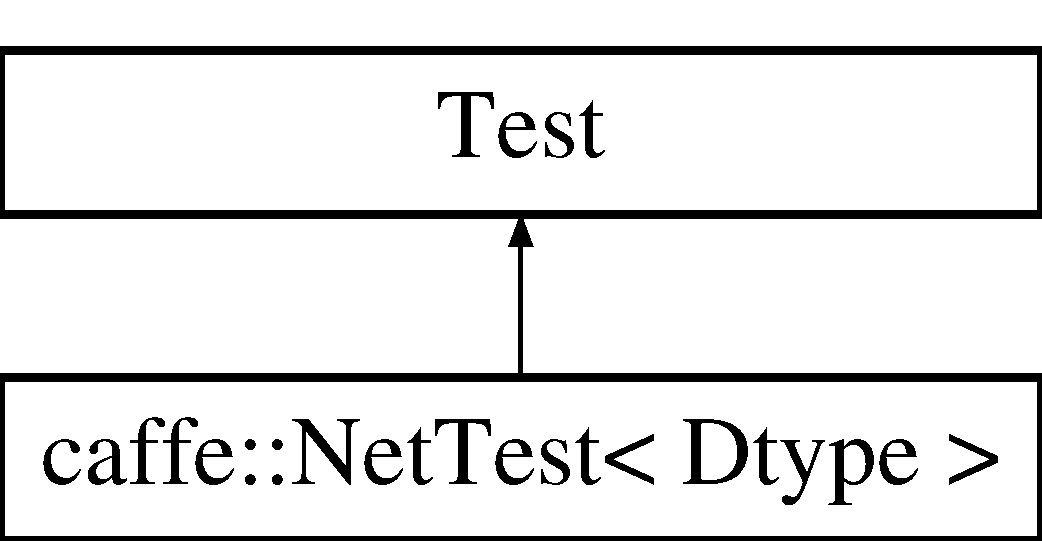
\includegraphics[height=2.000000cm]{classcaffe_1_1_net_test}
\end{center}
\end{figure}
\subsection*{Protected Member Functions}
\begin{DoxyCompactItemize}
\item 
virtual void \hyperlink{classcaffe_1_1_net_test_a5aa22b12f9902e216b3e056314465d97}{Set\+Up} ()
\end{DoxyCompactItemize}
\subsection*{Protected Attributes}
\begin{DoxyCompactItemize}
\item 
char $\ast$ \hyperlink{classcaffe_1_1_net_test_a8f238f38de09434b238b3bd3b518ad55}{filename\+\_\+}
\item 
string \hyperlink{classcaffe_1_1_net_test_ab797d941c20a3aa3beb52e1b190f01dd}{proto\+\_\+}
\end{DoxyCompactItemize}


\subsection{Member Function Documentation}
\hypertarget{classcaffe_1_1_net_test_a5aa22b12f9902e216b3e056314465d97}{\index{caffe\+::\+Net\+Test@{caffe\+::\+Net\+Test}!Set\+Up@{Set\+Up}}
\index{Set\+Up@{Set\+Up}!caffe\+::\+Net\+Test@{caffe\+::\+Net\+Test}}
\subsubsection[{Set\+Up}]{\setlength{\rightskip}{0pt plus 5cm}template$<$typename Dtype $>$ virtual void {\bf caffe\+::\+Net\+Test}$<$ Dtype $>$\+::Set\+Up (
\begin{DoxyParamCaption}
{}
\end{DoxyParamCaption}
)\hspace{0.3cm}{\ttfamily [inline]}, {\ttfamily [protected]}, {\ttfamily [virtual]}}}\label{classcaffe_1_1_net_test_a5aa22b12f9902e216b3e056314465d97}


\subsection{Member Data Documentation}
\hypertarget{classcaffe_1_1_net_test_a8f238f38de09434b238b3bd3b518ad55}{\index{caffe\+::\+Net\+Test@{caffe\+::\+Net\+Test}!filename\+\_\+@{filename\+\_\+}}
\index{filename\+\_\+@{filename\+\_\+}!caffe\+::\+Net\+Test@{caffe\+::\+Net\+Test}}
\subsubsection[{filename\+\_\+}]{\setlength{\rightskip}{0pt plus 5cm}template$<$typename Dtype $>$ char$\ast$ {\bf caffe\+::\+Net\+Test}$<$ Dtype $>$\+::filename\+\_\+\hspace{0.3cm}{\ttfamily [protected]}}}\label{classcaffe_1_1_net_test_a8f238f38de09434b238b3bd3b518ad55}
\hypertarget{classcaffe_1_1_net_test_ab797d941c20a3aa3beb52e1b190f01dd}{\index{caffe\+::\+Net\+Test@{caffe\+::\+Net\+Test}!proto\+\_\+@{proto\+\_\+}}
\index{proto\+\_\+@{proto\+\_\+}!caffe\+::\+Net\+Test@{caffe\+::\+Net\+Test}}
\subsubsection[{proto\+\_\+}]{\setlength{\rightskip}{0pt plus 5cm}template$<$typename Dtype $>$ string {\bf caffe\+::\+Net\+Test}$<$ Dtype $>$\+::proto\+\_\+\hspace{0.3cm}{\ttfamily [protected]}}}\label{classcaffe_1_1_net_test_ab797d941c20a3aa3beb52e1b190f01dd}


The documentation for this class was generated from the following file\+:\begin{DoxyCompactItemize}
\item 
src/caffe/test/\hyperlink{test__net_8cpp}{test\+\_\+net.\+cpp}\end{DoxyCompactItemize}

\hypertarget{classcaffe_1_1_neuron_layer}{\section{caffe\+:\+:Neuron\+Layer$<$ Dtype $>$ Class Template Reference}
\label{classcaffe_1_1_neuron_layer}\index{caffe\+::\+Neuron\+Layer$<$ Dtype $>$@{caffe\+::\+Neuron\+Layer$<$ Dtype $>$}}
}


{\ttfamily \#include $<$vision\+\_\+layers.\+hpp$>$}

Inheritance diagram for caffe\+:\+:Neuron\+Layer$<$ Dtype $>$\+:\begin{figure}[H]
\begin{center}
\leavevmode
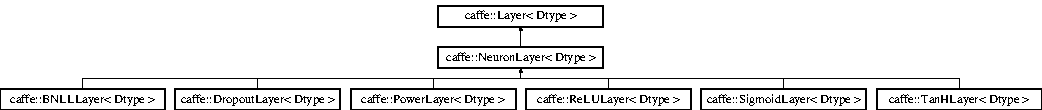
\includegraphics[height=1.473684cm]{classcaffe_1_1_neuron_layer}
\end{center}
\end{figure}
\subsection*{Public Member Functions}
\begin{DoxyCompactItemize}
\item 
\hyperlink{classcaffe_1_1_neuron_layer_a43348846697146ea9f01a773855b0915}{Neuron\+Layer} (const Layer\+Parameter \&param)
\item 
virtual void \hyperlink{classcaffe_1_1_neuron_layer_a8441089c3e6f2434a2683de22698352a}{Set\+Up} (const vector$<$ \hyperlink{classcaffe_1_1_blob}{Blob}$<$ Dtype $>$ $\ast$ $>$ \&bottom, vector$<$ \hyperlink{classcaffe_1_1_blob}{Blob}$<$ Dtype $>$ $\ast$ $>$ $\ast$top)
\end{DoxyCompactItemize}
\subsection*{Additional Inherited Members}


\subsection{Constructor \& Destructor Documentation}
\hypertarget{classcaffe_1_1_neuron_layer_a43348846697146ea9f01a773855b0915}{\index{caffe\+::\+Neuron\+Layer@{caffe\+::\+Neuron\+Layer}!Neuron\+Layer@{Neuron\+Layer}}
\index{Neuron\+Layer@{Neuron\+Layer}!caffe\+::\+Neuron\+Layer@{caffe\+::\+Neuron\+Layer}}
\subsubsection[{Neuron\+Layer}]{\setlength{\rightskip}{0pt plus 5cm}template$<$typename Dtype $>$ {\bf caffe\+::\+Neuron\+Layer}$<$ Dtype $>$\+::{\bf Neuron\+Layer} (
\begin{DoxyParamCaption}
\item[{const Layer\+Parameter \&}]{param}
\end{DoxyParamCaption}
)\hspace{0.3cm}{\ttfamily [inline]}, {\ttfamily [explicit]}}}\label{classcaffe_1_1_neuron_layer_a43348846697146ea9f01a773855b0915}


\subsection{Member Function Documentation}
\hypertarget{classcaffe_1_1_neuron_layer_a8441089c3e6f2434a2683de22698352a}{\index{caffe\+::\+Neuron\+Layer@{caffe\+::\+Neuron\+Layer}!Set\+Up@{Set\+Up}}
\index{Set\+Up@{Set\+Up}!caffe\+::\+Neuron\+Layer@{caffe\+::\+Neuron\+Layer}}
\subsubsection[{Set\+Up}]{\setlength{\rightskip}{0pt plus 5cm}template$<$typename Dtype $>$ void {\bf caffe\+::\+Neuron\+Layer}$<$ Dtype $>$\+::Set\+Up (
\begin{DoxyParamCaption}
\item[{const vector$<$ {\bf Blob}$<$ Dtype $>$ $\ast$ $>$ \&}]{bottom, }
\item[{vector$<$ {\bf Blob}$<$ Dtype $>$ $\ast$ $>$ $\ast$}]{top}
\end{DoxyParamCaption}
)\hspace{0.3cm}{\ttfamily [virtual]}}}\label{classcaffe_1_1_neuron_layer_a8441089c3e6f2434a2683de22698352a}


Implements \hyperlink{classcaffe_1_1_layer_abd13c6489c13953b4fbcfcf6880835d0}{caffe\+::\+Layer$<$ Dtype $>$}.



Reimplemented in \hyperlink{classcaffe_1_1_power_layer_a56719890adf4fbf31f1b63729a9a92f8}{caffe\+::\+Power\+Layer$<$ Dtype $>$}, and \hyperlink{classcaffe_1_1_dropout_layer_a1314d858640aa6ef2453c7cb6209be4e}{caffe\+::\+Dropout\+Layer$<$ Dtype $>$}.



The documentation for this class was generated from the following files\+:\begin{DoxyCompactItemize}
\item 
include/caffe/\hyperlink{vision__layers_8hpp}{vision\+\_\+layers.\+hpp}\item 
src/caffe/layers/\hyperlink{neuron__layer_8cpp}{neuron\+\_\+layer.\+cpp}\end{DoxyCompactItemize}

\hypertarget{classcaffe_1_1_neuron_layer_test}{\section{caffe\+:\+:Neuron\+Layer\+Test$<$ Dtype $>$ Class Template Reference}
\label{classcaffe_1_1_neuron_layer_test}\index{caffe\+::\+Neuron\+Layer\+Test$<$ Dtype $>$@{caffe\+::\+Neuron\+Layer\+Test$<$ Dtype $>$}}
}
Inheritance diagram for caffe\+:\+:Neuron\+Layer\+Test$<$ Dtype $>$\+:\begin{figure}[H]
\begin{center}
\leavevmode
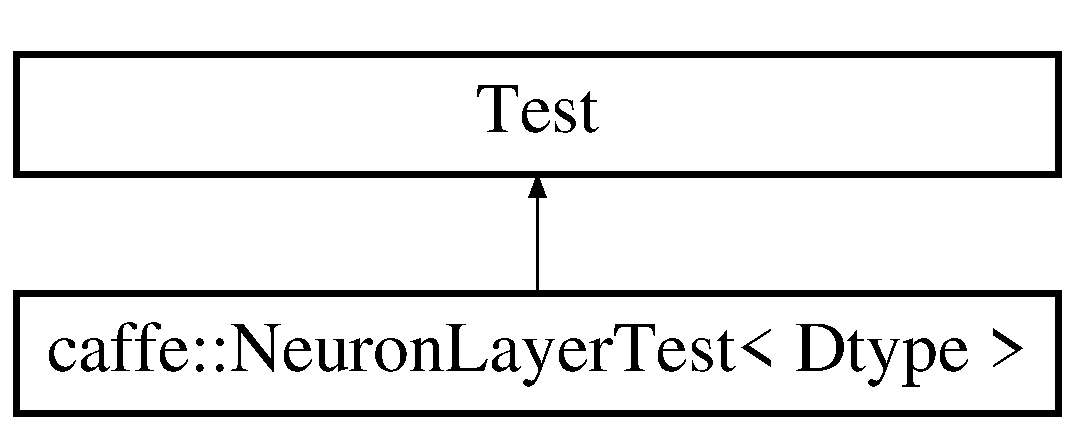
\includegraphics[height=2.000000cm]{classcaffe_1_1_neuron_layer_test}
\end{center}
\end{figure}
\subsection*{Protected Member Functions}
\begin{DoxyCompactItemize}
\item 
\hyperlink{classcaffe_1_1_neuron_layer_test_aee198daa132b0631250413df5b3ced74}{Neuron\+Layer\+Test} ()
\item 
virtual \hyperlink{classcaffe_1_1_neuron_layer_test_a2e16f0e3db0dad2f44db7d520252cefc}{$\sim$\+Neuron\+Layer\+Test} ()
\end{DoxyCompactItemize}
\subsection*{Protected Attributes}
\begin{DoxyCompactItemize}
\item 
\hyperlink{classcaffe_1_1_blob}{Blob}$<$ Dtype $>$ $\ast$const \hyperlink{classcaffe_1_1_neuron_layer_test_a54d0371564c8241de164e82e0af6102c}{blob\+\_\+bottom\+\_\+}
\item 
\hyperlink{classcaffe_1_1_blob}{Blob}$<$ Dtype $>$ $\ast$const \hyperlink{classcaffe_1_1_neuron_layer_test_a6e54ba573a61360912ab557ca0de7cfd}{blob\+\_\+top\+\_\+}
\item 
vector$<$ \hyperlink{classcaffe_1_1_blob}{Blob}$<$ Dtype $>$ $\ast$ $>$ \hyperlink{classcaffe_1_1_neuron_layer_test_afeee26d10841e52eea2c488dc0ac39b7}{blob\+\_\+bottom\+\_\+vec\+\_\+}
\item 
vector$<$ \hyperlink{classcaffe_1_1_blob}{Blob}$<$ Dtype $>$ $\ast$ $>$ \hyperlink{classcaffe_1_1_neuron_layer_test_a3d6414a30d5c5d16c64edc9b71da81e3}{blob\+\_\+top\+\_\+vec\+\_\+}
\end{DoxyCompactItemize}


\subsection{Constructor \& Destructor Documentation}
\hypertarget{classcaffe_1_1_neuron_layer_test_aee198daa132b0631250413df5b3ced74}{\index{caffe\+::\+Neuron\+Layer\+Test@{caffe\+::\+Neuron\+Layer\+Test}!Neuron\+Layer\+Test@{Neuron\+Layer\+Test}}
\index{Neuron\+Layer\+Test@{Neuron\+Layer\+Test}!caffe\+::\+Neuron\+Layer\+Test@{caffe\+::\+Neuron\+Layer\+Test}}
\subsubsection[{Neuron\+Layer\+Test}]{\setlength{\rightskip}{0pt plus 5cm}template$<$typename Dtype $>$ {\bf caffe\+::\+Neuron\+Layer\+Test}$<$ Dtype $>$\+::{\bf Neuron\+Layer\+Test} (
\begin{DoxyParamCaption}
{}
\end{DoxyParamCaption}
)\hspace{0.3cm}{\ttfamily [inline]}, {\ttfamily [protected]}}}\label{classcaffe_1_1_neuron_layer_test_aee198daa132b0631250413df5b3ced74}
\hypertarget{classcaffe_1_1_neuron_layer_test_a2e16f0e3db0dad2f44db7d520252cefc}{\index{caffe\+::\+Neuron\+Layer\+Test@{caffe\+::\+Neuron\+Layer\+Test}!````~Neuron\+Layer\+Test@{$\sim$\+Neuron\+Layer\+Test}}
\index{````~Neuron\+Layer\+Test@{$\sim$\+Neuron\+Layer\+Test}!caffe\+::\+Neuron\+Layer\+Test@{caffe\+::\+Neuron\+Layer\+Test}}
\subsubsection[{$\sim$\+Neuron\+Layer\+Test}]{\setlength{\rightskip}{0pt plus 5cm}template$<$typename Dtype $>$ virtual {\bf caffe\+::\+Neuron\+Layer\+Test}$<$ Dtype $>$\+::$\sim${\bf Neuron\+Layer\+Test} (
\begin{DoxyParamCaption}
{}
\end{DoxyParamCaption}
)\hspace{0.3cm}{\ttfamily [inline]}, {\ttfamily [protected]}, {\ttfamily [virtual]}}}\label{classcaffe_1_1_neuron_layer_test_a2e16f0e3db0dad2f44db7d520252cefc}


\subsection{Member Data Documentation}
\hypertarget{classcaffe_1_1_neuron_layer_test_a54d0371564c8241de164e82e0af6102c}{\index{caffe\+::\+Neuron\+Layer\+Test@{caffe\+::\+Neuron\+Layer\+Test}!blob\+\_\+bottom\+\_\+@{blob\+\_\+bottom\+\_\+}}
\index{blob\+\_\+bottom\+\_\+@{blob\+\_\+bottom\+\_\+}!caffe\+::\+Neuron\+Layer\+Test@{caffe\+::\+Neuron\+Layer\+Test}}
\subsubsection[{blob\+\_\+bottom\+\_\+}]{\setlength{\rightskip}{0pt plus 5cm}template$<$typename Dtype $>$ {\bf Blob}$<$Dtype$>$$\ast$ const {\bf caffe\+::\+Neuron\+Layer\+Test}$<$ Dtype $>$\+::blob\+\_\+bottom\+\_\+\hspace{0.3cm}{\ttfamily [protected]}}}\label{classcaffe_1_1_neuron_layer_test_a54d0371564c8241de164e82e0af6102c}
\hypertarget{classcaffe_1_1_neuron_layer_test_afeee26d10841e52eea2c488dc0ac39b7}{\index{caffe\+::\+Neuron\+Layer\+Test@{caffe\+::\+Neuron\+Layer\+Test}!blob\+\_\+bottom\+\_\+vec\+\_\+@{blob\+\_\+bottom\+\_\+vec\+\_\+}}
\index{blob\+\_\+bottom\+\_\+vec\+\_\+@{blob\+\_\+bottom\+\_\+vec\+\_\+}!caffe\+::\+Neuron\+Layer\+Test@{caffe\+::\+Neuron\+Layer\+Test}}
\subsubsection[{blob\+\_\+bottom\+\_\+vec\+\_\+}]{\setlength{\rightskip}{0pt plus 5cm}template$<$typename Dtype $>$ vector$<${\bf Blob}$<$Dtype$>$$\ast$$>$ {\bf caffe\+::\+Neuron\+Layer\+Test}$<$ Dtype $>$\+::blob\+\_\+bottom\+\_\+vec\+\_\+\hspace{0.3cm}{\ttfamily [protected]}}}\label{classcaffe_1_1_neuron_layer_test_afeee26d10841e52eea2c488dc0ac39b7}
\hypertarget{classcaffe_1_1_neuron_layer_test_a6e54ba573a61360912ab557ca0de7cfd}{\index{caffe\+::\+Neuron\+Layer\+Test@{caffe\+::\+Neuron\+Layer\+Test}!blob\+\_\+top\+\_\+@{blob\+\_\+top\+\_\+}}
\index{blob\+\_\+top\+\_\+@{blob\+\_\+top\+\_\+}!caffe\+::\+Neuron\+Layer\+Test@{caffe\+::\+Neuron\+Layer\+Test}}
\subsubsection[{blob\+\_\+top\+\_\+}]{\setlength{\rightskip}{0pt plus 5cm}template$<$typename Dtype $>$ {\bf Blob}$<$Dtype$>$$\ast$ const {\bf caffe\+::\+Neuron\+Layer\+Test}$<$ Dtype $>$\+::blob\+\_\+top\+\_\+\hspace{0.3cm}{\ttfamily [protected]}}}\label{classcaffe_1_1_neuron_layer_test_a6e54ba573a61360912ab557ca0de7cfd}
\hypertarget{classcaffe_1_1_neuron_layer_test_a3d6414a30d5c5d16c64edc9b71da81e3}{\index{caffe\+::\+Neuron\+Layer\+Test@{caffe\+::\+Neuron\+Layer\+Test}!blob\+\_\+top\+\_\+vec\+\_\+@{blob\+\_\+top\+\_\+vec\+\_\+}}
\index{blob\+\_\+top\+\_\+vec\+\_\+@{blob\+\_\+top\+\_\+vec\+\_\+}!caffe\+::\+Neuron\+Layer\+Test@{caffe\+::\+Neuron\+Layer\+Test}}
\subsubsection[{blob\+\_\+top\+\_\+vec\+\_\+}]{\setlength{\rightskip}{0pt plus 5cm}template$<$typename Dtype $>$ vector$<${\bf Blob}$<$Dtype$>$$\ast$$>$ {\bf caffe\+::\+Neuron\+Layer\+Test}$<$ Dtype $>$\+::blob\+\_\+top\+\_\+vec\+\_\+\hspace{0.3cm}{\ttfamily [protected]}}}\label{classcaffe_1_1_neuron_layer_test_a3d6414a30d5c5d16c64edc9b71da81e3}


The documentation for this class was generated from the following file\+:\begin{DoxyCompactItemize}
\item 
src/caffe/test/\hyperlink{test__neuron__layer_8cpp}{test\+\_\+neuron\+\_\+layer.\+cpp}\end{DoxyCompactItemize}

\hypertarget{classcaffe_1_1_padding_layer_upgrade_test}{\section{caffe\+:\+:Padding\+Layer\+Upgrade\+Test Class Reference}
\label{classcaffe_1_1_padding_layer_upgrade_test}\index{caffe\+::\+Padding\+Layer\+Upgrade\+Test@{caffe\+::\+Padding\+Layer\+Upgrade\+Test}}
}
Inheritance diagram for caffe\+:\+:Padding\+Layer\+Upgrade\+Test\+:\begin{figure}[H]
\begin{center}
\leavevmode
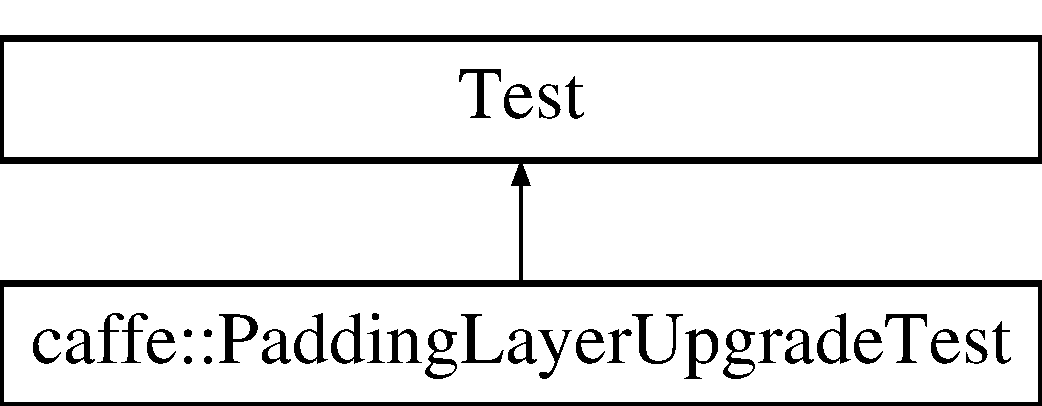
\includegraphics[height=2.000000cm]{classcaffe_1_1_padding_layer_upgrade_test}
\end{center}
\end{figure}
\subsection*{Protected Member Functions}
\begin{DoxyCompactItemize}
\item 
void \hyperlink{classcaffe_1_1_padding_layer_upgrade_test_aba08eb6766f8d55f30f66d5549f42147}{Run\+Padding\+Upgrade\+Test} (const string \&input\+\_\+param\+\_\+string, const string \&output\+\_\+param\+\_\+string)
\end{DoxyCompactItemize}


\subsection{Member Function Documentation}
\hypertarget{classcaffe_1_1_padding_layer_upgrade_test_aba08eb6766f8d55f30f66d5549f42147}{\index{caffe\+::\+Padding\+Layer\+Upgrade\+Test@{caffe\+::\+Padding\+Layer\+Upgrade\+Test}!Run\+Padding\+Upgrade\+Test@{Run\+Padding\+Upgrade\+Test}}
\index{Run\+Padding\+Upgrade\+Test@{Run\+Padding\+Upgrade\+Test}!caffe\+::\+Padding\+Layer\+Upgrade\+Test@{caffe\+::\+Padding\+Layer\+Upgrade\+Test}}
\subsubsection[{Run\+Padding\+Upgrade\+Test}]{\setlength{\rightskip}{0pt plus 5cm}void caffe\+::\+Padding\+Layer\+Upgrade\+Test\+::\+Run\+Padding\+Upgrade\+Test (
\begin{DoxyParamCaption}
\item[{const string \&}]{input\+\_\+param\+\_\+string, }
\item[{const string \&}]{output\+\_\+param\+\_\+string}
\end{DoxyParamCaption}
)\hspace{0.3cm}{\ttfamily [inline]}, {\ttfamily [protected]}}}\label{classcaffe_1_1_padding_layer_upgrade_test_aba08eb6766f8d55f30f66d5549f42147}


The documentation for this class was generated from the following file\+:\begin{DoxyCompactItemize}
\item 
src/caffe/test/\hyperlink{test__upgrade__proto_8cpp}{test\+\_\+upgrade\+\_\+proto.\+cpp}\end{DoxyCompactItemize}

\hypertarget{classcaffe_1_1_platform_test}{\section{caffe\+:\+:Platform\+Test Class Reference}
\label{classcaffe_1_1_platform_test}\index{caffe\+::\+Platform\+Test@{caffe\+::\+Platform\+Test}}
}
Inheritance diagram for caffe\+:\+:Platform\+Test\+:\begin{figure}[H]
\begin{center}
\leavevmode
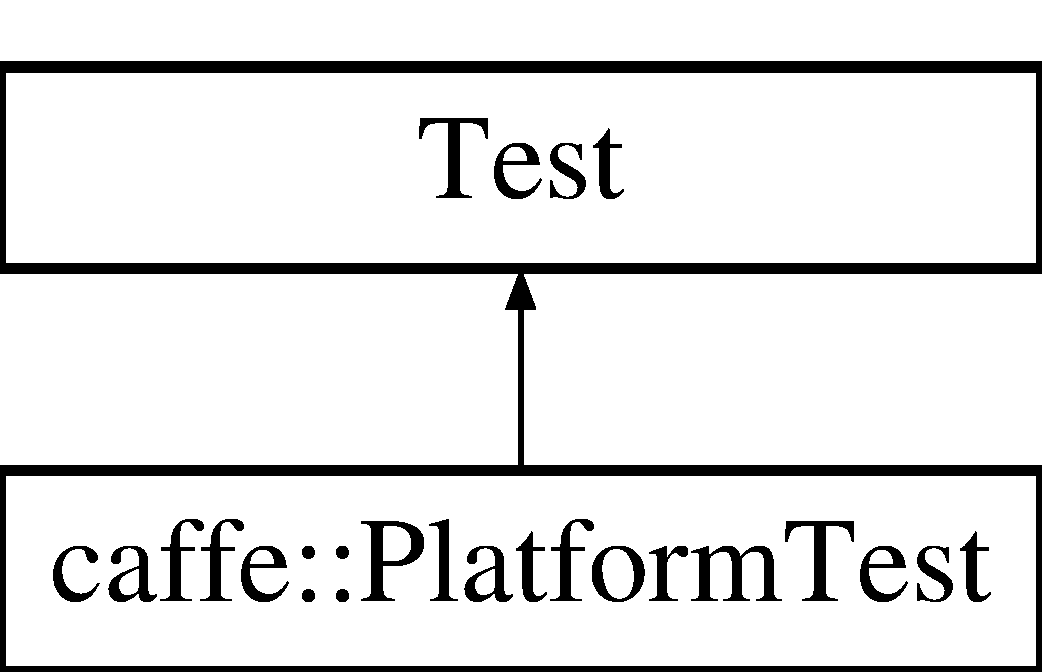
\includegraphics[height=2.000000cm]{classcaffe_1_1_platform_test}
\end{center}
\end{figure}


The documentation for this class was generated from the following file\+:\begin{DoxyCompactItemize}
\item 
src/caffe/test/\hyperlink{test__platform_8cpp}{test\+\_\+platform.\+cpp}\end{DoxyCompactItemize}

\hypertarget{classcaffe_1_1_pooling_layer}{\section{caffe\+:\+:Pooling\+Layer$<$ Dtype $>$ Class Template Reference}
\label{classcaffe_1_1_pooling_layer}\index{caffe\+::\+Pooling\+Layer$<$ Dtype $>$@{caffe\+::\+Pooling\+Layer$<$ Dtype $>$}}
}


{\ttfamily \#include $<$vision\+\_\+layers.\+hpp$>$}

Inheritance diagram for caffe\+:\+:Pooling\+Layer$<$ Dtype $>$\+:\begin{figure}[H]
\begin{center}
\leavevmode
\includegraphics[height=2.000000cm]{classcaffe_1_1_pooling_layer}
\end{center}
\end{figure}
\subsection*{Public Member Functions}
\begin{DoxyCompactItemize}
\item 
\hyperlink{classcaffe_1_1_pooling_layer_a3bc79b6101f5e21bbbfa02b7726d650c}{Pooling\+Layer} (const Layer\+Parameter \&param)
\item 
virtual void \hyperlink{classcaffe_1_1_pooling_layer_ac88da7bd4cb54fceb0a22a6efc61292e}{Set\+Up} (const vector$<$ \hyperlink{classcaffe_1_1_blob}{Blob}$<$ Dtype $>$ $\ast$ $>$ \&bottom, vector$<$ \hyperlink{classcaffe_1_1_blob}{Blob}$<$ Dtype $>$ $\ast$ $>$ $\ast$top)
\end{DoxyCompactItemize}
\subsection*{Protected Member Functions}
\begin{DoxyCompactItemize}
\item 
virtual Dtype \hyperlink{classcaffe_1_1_pooling_layer_a94e0eecfd992d045bd0b8b0cee4523f0}{Forward\+\_\+cpu} (const vector$<$ \hyperlink{classcaffe_1_1_blob}{Blob}$<$ Dtype $>$ $\ast$ $>$ \&bottom, vector$<$ \hyperlink{classcaffe_1_1_blob}{Blob}$<$ Dtype $>$ $\ast$ $>$ $\ast$top)
\item 
virtual Dtype \hyperlink{classcaffe_1_1_pooling_layer_a6997ba2f8adca32e201b2e3aa5271791}{Forward\+\_\+gpu} (const vector$<$ \hyperlink{classcaffe_1_1_blob}{Blob}$<$ Dtype $>$ $\ast$ $>$ \&bottom, vector$<$ \hyperlink{classcaffe_1_1_blob}{Blob}$<$ Dtype $>$ $\ast$ $>$ $\ast$top)
\item 
virtual void \hyperlink{classcaffe_1_1_pooling_layer_aad07e6ab8b23155a971e2e78e87f0763}{Backward\+\_\+cpu} (const vector$<$ \hyperlink{classcaffe_1_1_blob}{Blob}$<$ Dtype $>$ $\ast$ $>$ \&top, const bool propagate\+\_\+down, vector$<$ \hyperlink{classcaffe_1_1_blob}{Blob}$<$ Dtype $>$ $\ast$ $>$ $\ast$bottom)
\item 
virtual void \hyperlink{classcaffe_1_1_pooling_layer_a90db5feba107ee64fb1c3cfacc0b2f38}{Backward\+\_\+gpu} (const vector$<$ \hyperlink{classcaffe_1_1_blob}{Blob}$<$ Dtype $>$ $\ast$ $>$ \&top, const bool propagate\+\_\+down, vector$<$ \hyperlink{classcaffe_1_1_blob}{Blob}$<$ Dtype $>$ $\ast$ $>$ $\ast$bottom)
\end{DoxyCompactItemize}
\subsection*{Protected Attributes}
\begin{DoxyCompactItemize}
\item 
int \hyperlink{classcaffe_1_1_pooling_layer_a93e497a4fe4888f74dec455b7b030cb1}{kernel\+\_\+size\+\_\+}
\item 
int \hyperlink{classcaffe_1_1_pooling_layer_a8ae76d095f5e31218fd79ec62b99f4f3}{stride\+\_\+}
\item 
int \hyperlink{classcaffe_1_1_pooling_layer_a9427e9a29b2b573ac8b34501344d0540}{pad\+\_\+}
\item 
int \hyperlink{classcaffe_1_1_pooling_layer_a9aaf4e65127d969b32b1a860dcb380f4}{channels\+\_\+}
\item 
int \hyperlink{classcaffe_1_1_pooling_layer_a58ef04bbd1ee89201b07f99329538e95}{height\+\_\+}
\item 
int \hyperlink{classcaffe_1_1_pooling_layer_a812efd53d8f67f250beeb7c79cc74cbe}{width\+\_\+}
\item 
int \hyperlink{classcaffe_1_1_pooling_layer_a21f1550ebe8a4b2a6731a7c871e1bda8}{pooled\+\_\+height\+\_\+}
\item 
int \hyperlink{classcaffe_1_1_pooling_layer_a73ddab9147f6ad736938a55a2dc74a0d}{pooled\+\_\+width\+\_\+}
\item 
\hyperlink{classcaffe_1_1_blob}{Blob}$<$ Dtype $>$ \hyperlink{classcaffe_1_1_pooling_layer_a03c023517f2f74771d6da233b161964a}{rand\+\_\+idx\+\_\+}
\end{DoxyCompactItemize}


\subsection{Constructor \& Destructor Documentation}
\hypertarget{classcaffe_1_1_pooling_layer_a3bc79b6101f5e21bbbfa02b7726d650c}{\index{caffe\+::\+Pooling\+Layer@{caffe\+::\+Pooling\+Layer}!Pooling\+Layer@{Pooling\+Layer}}
\index{Pooling\+Layer@{Pooling\+Layer}!caffe\+::\+Pooling\+Layer@{caffe\+::\+Pooling\+Layer}}
\subsubsection[{Pooling\+Layer}]{\setlength{\rightskip}{0pt plus 5cm}template$<$typename Dtype $>$ {\bf caffe\+::\+Pooling\+Layer}$<$ Dtype $>$\+::{\bf Pooling\+Layer} (
\begin{DoxyParamCaption}
\item[{const Layer\+Parameter \&}]{param}
\end{DoxyParamCaption}
)\hspace{0.3cm}{\ttfamily [inline]}, {\ttfamily [explicit]}}}\label{classcaffe_1_1_pooling_layer_a3bc79b6101f5e21bbbfa02b7726d650c}


\subsection{Member Function Documentation}
\hypertarget{classcaffe_1_1_pooling_layer_aad07e6ab8b23155a971e2e78e87f0763}{\index{caffe\+::\+Pooling\+Layer@{caffe\+::\+Pooling\+Layer}!Backward\+\_\+cpu@{Backward\+\_\+cpu}}
\index{Backward\+\_\+cpu@{Backward\+\_\+cpu}!caffe\+::\+Pooling\+Layer@{caffe\+::\+Pooling\+Layer}}
\subsubsection[{Backward\+\_\+cpu}]{\setlength{\rightskip}{0pt plus 5cm}template$<$typename Dtype $>$ void {\bf caffe\+::\+Pooling\+Layer}$<$ Dtype $>$\+::Backward\+\_\+cpu (
\begin{DoxyParamCaption}
\item[{const vector$<$ {\bf Blob}$<$ Dtype $>$ $\ast$ $>$ \&}]{top, }
\item[{const bool}]{propagate\+\_\+down, }
\item[{vector$<$ {\bf Blob}$<$ Dtype $>$ $\ast$ $>$ $\ast$}]{bottom}
\end{DoxyParamCaption}
)\hspace{0.3cm}{\ttfamily [protected]}, {\ttfamily [virtual]}}}\label{classcaffe_1_1_pooling_layer_aad07e6ab8b23155a971e2e78e87f0763}


Implements \hyperlink{classcaffe_1_1_layer_ac2d82011d076237c67997f63e7ee4b80}{caffe\+::\+Layer$<$ Dtype $>$}.

\hypertarget{classcaffe_1_1_pooling_layer_a90db5feba107ee64fb1c3cfacc0b2f38}{\index{caffe\+::\+Pooling\+Layer@{caffe\+::\+Pooling\+Layer}!Backward\+\_\+gpu@{Backward\+\_\+gpu}}
\index{Backward\+\_\+gpu@{Backward\+\_\+gpu}!caffe\+::\+Pooling\+Layer@{caffe\+::\+Pooling\+Layer}}
\subsubsection[{Backward\+\_\+gpu}]{\setlength{\rightskip}{0pt plus 5cm}template$<$typename Dtype $>$ void {\bf caffe\+::\+Pooling\+Layer}$<$ Dtype $>$\+::Backward\+\_\+gpu (
\begin{DoxyParamCaption}
\item[{const vector$<$ {\bf Blob}$<$ Dtype $>$ $\ast$ $>$ \&}]{top, }
\item[{const bool}]{propagate\+\_\+down, }
\item[{vector$<$ {\bf Blob}$<$ Dtype $>$ $\ast$ $>$ $\ast$}]{bottom}
\end{DoxyParamCaption}
)\hspace{0.3cm}{\ttfamily [protected]}, {\ttfamily [virtual]}}}\label{classcaffe_1_1_pooling_layer_a90db5feba107ee64fb1c3cfacc0b2f38}


Reimplemented from \hyperlink{classcaffe_1_1_layer_adf07ffe1f22d2fd2b1b0ff475ef5a64b}{caffe\+::\+Layer$<$ Dtype $>$}.

\hypertarget{classcaffe_1_1_pooling_layer_a94e0eecfd992d045bd0b8b0cee4523f0}{\index{caffe\+::\+Pooling\+Layer@{caffe\+::\+Pooling\+Layer}!Forward\+\_\+cpu@{Forward\+\_\+cpu}}
\index{Forward\+\_\+cpu@{Forward\+\_\+cpu}!caffe\+::\+Pooling\+Layer@{caffe\+::\+Pooling\+Layer}}
\subsubsection[{Forward\+\_\+cpu}]{\setlength{\rightskip}{0pt plus 5cm}template$<$typename Dtype $>$ Dtype {\bf caffe\+::\+Pooling\+Layer}$<$ Dtype $>$\+::Forward\+\_\+cpu (
\begin{DoxyParamCaption}
\item[{const vector$<$ {\bf Blob}$<$ Dtype $>$ $\ast$ $>$ \&}]{bottom, }
\item[{vector$<$ {\bf Blob}$<$ Dtype $>$ $\ast$ $>$ $\ast$}]{top}
\end{DoxyParamCaption}
)\hspace{0.3cm}{\ttfamily [protected]}, {\ttfamily [virtual]}}}\label{classcaffe_1_1_pooling_layer_a94e0eecfd992d045bd0b8b0cee4523f0}


Implements \hyperlink{classcaffe_1_1_layer_a8f7f61da3b8b3ca7f2394dee33873353}{caffe\+::\+Layer$<$ Dtype $>$}.

\hypertarget{classcaffe_1_1_pooling_layer_a6997ba2f8adca32e201b2e3aa5271791}{\index{caffe\+::\+Pooling\+Layer@{caffe\+::\+Pooling\+Layer}!Forward\+\_\+gpu@{Forward\+\_\+gpu}}
\index{Forward\+\_\+gpu@{Forward\+\_\+gpu}!caffe\+::\+Pooling\+Layer@{caffe\+::\+Pooling\+Layer}}
\subsubsection[{Forward\+\_\+gpu}]{\setlength{\rightskip}{0pt plus 5cm}template$<$typename Dtype $>$ Dtype {\bf caffe\+::\+Pooling\+Layer}$<$ Dtype $>$\+::Forward\+\_\+gpu (
\begin{DoxyParamCaption}
\item[{const vector$<$ {\bf Blob}$<$ Dtype $>$ $\ast$ $>$ \&}]{bottom, }
\item[{vector$<$ {\bf Blob}$<$ Dtype $>$ $\ast$ $>$ $\ast$}]{top}
\end{DoxyParamCaption}
)\hspace{0.3cm}{\ttfamily [protected]}, {\ttfamily [virtual]}}}\label{classcaffe_1_1_pooling_layer_a6997ba2f8adca32e201b2e3aa5271791}


Reimplemented from \hyperlink{classcaffe_1_1_layer_a2d78dbf5d8bc36928bd8f6fcfbafbcef}{caffe\+::\+Layer$<$ Dtype $>$}.

\hypertarget{classcaffe_1_1_pooling_layer_ac88da7bd4cb54fceb0a22a6efc61292e}{\index{caffe\+::\+Pooling\+Layer@{caffe\+::\+Pooling\+Layer}!Set\+Up@{Set\+Up}}
\index{Set\+Up@{Set\+Up}!caffe\+::\+Pooling\+Layer@{caffe\+::\+Pooling\+Layer}}
\subsubsection[{Set\+Up}]{\setlength{\rightskip}{0pt plus 5cm}template$<$typename Dtype $>$ void {\bf caffe\+::\+Pooling\+Layer}$<$ Dtype $>$\+::Set\+Up (
\begin{DoxyParamCaption}
\item[{const vector$<$ {\bf Blob}$<$ Dtype $>$ $\ast$ $>$ \&}]{bottom, }
\item[{vector$<$ {\bf Blob}$<$ Dtype $>$ $\ast$ $>$ $\ast$}]{top}
\end{DoxyParamCaption}
)\hspace{0.3cm}{\ttfamily [virtual]}}}\label{classcaffe_1_1_pooling_layer_ac88da7bd4cb54fceb0a22a6efc61292e}


Implements \hyperlink{classcaffe_1_1_layer_abd13c6489c13953b4fbcfcf6880835d0}{caffe\+::\+Layer$<$ Dtype $>$}.



\subsection{Member Data Documentation}
\hypertarget{classcaffe_1_1_pooling_layer_a9aaf4e65127d969b32b1a860dcb380f4}{\index{caffe\+::\+Pooling\+Layer@{caffe\+::\+Pooling\+Layer}!channels\+\_\+@{channels\+\_\+}}
\index{channels\+\_\+@{channels\+\_\+}!caffe\+::\+Pooling\+Layer@{caffe\+::\+Pooling\+Layer}}
\subsubsection[{channels\+\_\+}]{\setlength{\rightskip}{0pt plus 5cm}template$<$typename Dtype $>$ int {\bf caffe\+::\+Pooling\+Layer}$<$ Dtype $>$\+::channels\+\_\+\hspace{0.3cm}{\ttfamily [protected]}}}\label{classcaffe_1_1_pooling_layer_a9aaf4e65127d969b32b1a860dcb380f4}
\hypertarget{classcaffe_1_1_pooling_layer_a58ef04bbd1ee89201b07f99329538e95}{\index{caffe\+::\+Pooling\+Layer@{caffe\+::\+Pooling\+Layer}!height\+\_\+@{height\+\_\+}}
\index{height\+\_\+@{height\+\_\+}!caffe\+::\+Pooling\+Layer@{caffe\+::\+Pooling\+Layer}}
\subsubsection[{height\+\_\+}]{\setlength{\rightskip}{0pt plus 5cm}template$<$typename Dtype $>$ int {\bf caffe\+::\+Pooling\+Layer}$<$ Dtype $>$\+::height\+\_\+\hspace{0.3cm}{\ttfamily [protected]}}}\label{classcaffe_1_1_pooling_layer_a58ef04bbd1ee89201b07f99329538e95}
\hypertarget{classcaffe_1_1_pooling_layer_a93e497a4fe4888f74dec455b7b030cb1}{\index{caffe\+::\+Pooling\+Layer@{caffe\+::\+Pooling\+Layer}!kernel\+\_\+size\+\_\+@{kernel\+\_\+size\+\_\+}}
\index{kernel\+\_\+size\+\_\+@{kernel\+\_\+size\+\_\+}!caffe\+::\+Pooling\+Layer@{caffe\+::\+Pooling\+Layer}}
\subsubsection[{kernel\+\_\+size\+\_\+}]{\setlength{\rightskip}{0pt plus 5cm}template$<$typename Dtype $>$ int {\bf caffe\+::\+Pooling\+Layer}$<$ Dtype $>$\+::kernel\+\_\+size\+\_\+\hspace{0.3cm}{\ttfamily [protected]}}}\label{classcaffe_1_1_pooling_layer_a93e497a4fe4888f74dec455b7b030cb1}
\hypertarget{classcaffe_1_1_pooling_layer_a9427e9a29b2b573ac8b34501344d0540}{\index{caffe\+::\+Pooling\+Layer@{caffe\+::\+Pooling\+Layer}!pad\+\_\+@{pad\+\_\+}}
\index{pad\+\_\+@{pad\+\_\+}!caffe\+::\+Pooling\+Layer@{caffe\+::\+Pooling\+Layer}}
\subsubsection[{pad\+\_\+}]{\setlength{\rightskip}{0pt plus 5cm}template$<$typename Dtype $>$ int {\bf caffe\+::\+Pooling\+Layer}$<$ Dtype $>$\+::pad\+\_\+\hspace{0.3cm}{\ttfamily [protected]}}}\label{classcaffe_1_1_pooling_layer_a9427e9a29b2b573ac8b34501344d0540}
\hypertarget{classcaffe_1_1_pooling_layer_a21f1550ebe8a4b2a6731a7c871e1bda8}{\index{caffe\+::\+Pooling\+Layer@{caffe\+::\+Pooling\+Layer}!pooled\+\_\+height\+\_\+@{pooled\+\_\+height\+\_\+}}
\index{pooled\+\_\+height\+\_\+@{pooled\+\_\+height\+\_\+}!caffe\+::\+Pooling\+Layer@{caffe\+::\+Pooling\+Layer}}
\subsubsection[{pooled\+\_\+height\+\_\+}]{\setlength{\rightskip}{0pt plus 5cm}template$<$typename Dtype $>$ int {\bf caffe\+::\+Pooling\+Layer}$<$ Dtype $>$\+::pooled\+\_\+height\+\_\+\hspace{0.3cm}{\ttfamily [protected]}}}\label{classcaffe_1_1_pooling_layer_a21f1550ebe8a4b2a6731a7c871e1bda8}
\hypertarget{classcaffe_1_1_pooling_layer_a73ddab9147f6ad736938a55a2dc74a0d}{\index{caffe\+::\+Pooling\+Layer@{caffe\+::\+Pooling\+Layer}!pooled\+\_\+width\+\_\+@{pooled\+\_\+width\+\_\+}}
\index{pooled\+\_\+width\+\_\+@{pooled\+\_\+width\+\_\+}!caffe\+::\+Pooling\+Layer@{caffe\+::\+Pooling\+Layer}}
\subsubsection[{pooled\+\_\+width\+\_\+}]{\setlength{\rightskip}{0pt plus 5cm}template$<$typename Dtype $>$ int {\bf caffe\+::\+Pooling\+Layer}$<$ Dtype $>$\+::pooled\+\_\+width\+\_\+\hspace{0.3cm}{\ttfamily [protected]}}}\label{classcaffe_1_1_pooling_layer_a73ddab9147f6ad736938a55a2dc74a0d}
\hypertarget{classcaffe_1_1_pooling_layer_a03c023517f2f74771d6da233b161964a}{\index{caffe\+::\+Pooling\+Layer@{caffe\+::\+Pooling\+Layer}!rand\+\_\+idx\+\_\+@{rand\+\_\+idx\+\_\+}}
\index{rand\+\_\+idx\+\_\+@{rand\+\_\+idx\+\_\+}!caffe\+::\+Pooling\+Layer@{caffe\+::\+Pooling\+Layer}}
\subsubsection[{rand\+\_\+idx\+\_\+}]{\setlength{\rightskip}{0pt plus 5cm}template$<$typename Dtype $>$ {\bf Blob}$<$Dtype$>$ {\bf caffe\+::\+Pooling\+Layer}$<$ Dtype $>$\+::rand\+\_\+idx\+\_\+\hspace{0.3cm}{\ttfamily [protected]}}}\label{classcaffe_1_1_pooling_layer_a03c023517f2f74771d6da233b161964a}
\hypertarget{classcaffe_1_1_pooling_layer_a8ae76d095f5e31218fd79ec62b99f4f3}{\index{caffe\+::\+Pooling\+Layer@{caffe\+::\+Pooling\+Layer}!stride\+\_\+@{stride\+\_\+}}
\index{stride\+\_\+@{stride\+\_\+}!caffe\+::\+Pooling\+Layer@{caffe\+::\+Pooling\+Layer}}
\subsubsection[{stride\+\_\+}]{\setlength{\rightskip}{0pt plus 5cm}template$<$typename Dtype $>$ int {\bf caffe\+::\+Pooling\+Layer}$<$ Dtype $>$\+::stride\+\_\+\hspace{0.3cm}{\ttfamily [protected]}}}\label{classcaffe_1_1_pooling_layer_a8ae76d095f5e31218fd79ec62b99f4f3}
\hypertarget{classcaffe_1_1_pooling_layer_a812efd53d8f67f250beeb7c79cc74cbe}{\index{caffe\+::\+Pooling\+Layer@{caffe\+::\+Pooling\+Layer}!width\+\_\+@{width\+\_\+}}
\index{width\+\_\+@{width\+\_\+}!caffe\+::\+Pooling\+Layer@{caffe\+::\+Pooling\+Layer}}
\subsubsection[{width\+\_\+}]{\setlength{\rightskip}{0pt plus 5cm}template$<$typename Dtype $>$ int {\bf caffe\+::\+Pooling\+Layer}$<$ Dtype $>$\+::width\+\_\+\hspace{0.3cm}{\ttfamily [protected]}}}\label{classcaffe_1_1_pooling_layer_a812efd53d8f67f250beeb7c79cc74cbe}


The documentation for this class was generated from the following files\+:\begin{DoxyCompactItemize}
\item 
include/caffe/\hyperlink{vision__layers_8hpp}{vision\+\_\+layers.\+hpp}\item 
src/caffe/layers/\hyperlink{pooling__layer_8cpp}{pooling\+\_\+layer.\+cpp}\item 
src/caffe/layers/\hyperlink{pooling__layer_8cu}{pooling\+\_\+layer.\+cu}\end{DoxyCompactItemize}

\hypertarget{classcaffe_1_1_pooling_layer_test}{\section{caffe\+:\+:Pooling\+Layer\+Test$<$ Dtype $>$ Class Template Reference}
\label{classcaffe_1_1_pooling_layer_test}\index{caffe\+::\+Pooling\+Layer\+Test$<$ Dtype $>$@{caffe\+::\+Pooling\+Layer\+Test$<$ Dtype $>$}}
}
Inheritance diagram for caffe\+:\+:Pooling\+Layer\+Test$<$ Dtype $>$\+:\begin{figure}[H]
\begin{center}
\leavevmode
\includegraphics[height=2.000000cm]{classcaffe_1_1_pooling_layer_test}
\end{center}
\end{figure}
\subsection*{Protected Member Functions}
\begin{DoxyCompactItemize}
\item 
\hyperlink{classcaffe_1_1_pooling_layer_test_a7742eacaa14ae7a01fed87b54ee5bdd1}{Pooling\+Layer\+Test} ()
\item 
virtual void \hyperlink{classcaffe_1_1_pooling_layer_test_a814208159f9155a7d28cfe289fe1414c}{Set\+Up} ()
\item 
virtual \hyperlink{classcaffe_1_1_pooling_layer_test_a9575a28a7718df9a3e77d6984b9f8f46}{$\sim$\+Pooling\+Layer\+Test} ()
\end{DoxyCompactItemize}
\subsection*{Protected Attributes}
\begin{DoxyCompactItemize}
\item 
\hyperlink{classcaffe_1_1_blob}{Blob}$<$ Dtype $>$ $\ast$const \hyperlink{classcaffe_1_1_pooling_layer_test_ad6228ca6fb50a4e589f18fd314be0019}{blob\+\_\+bottom\+\_\+}
\item 
\hyperlink{classcaffe_1_1_blob}{Blob}$<$ Dtype $>$ $\ast$const \hyperlink{classcaffe_1_1_pooling_layer_test_aadabc8d33eec24086aedbf96c963518c}{blob\+\_\+top\+\_\+}
\item 
vector$<$ \hyperlink{classcaffe_1_1_blob}{Blob}$<$ Dtype $>$ $\ast$ $>$ \hyperlink{classcaffe_1_1_pooling_layer_test_a4441920a9bb7a9e7aac0a7298da8b13b}{blob\+\_\+bottom\+\_\+vec\+\_\+}
\item 
vector$<$ \hyperlink{classcaffe_1_1_blob}{Blob}$<$ Dtype $>$ $\ast$ $>$ \hyperlink{classcaffe_1_1_pooling_layer_test_a9ffa0628b08c6223f2f8fd4646ef0aca}{blob\+\_\+top\+\_\+vec\+\_\+}
\end{DoxyCompactItemize}


\subsection{Constructor \& Destructor Documentation}
\hypertarget{classcaffe_1_1_pooling_layer_test_a7742eacaa14ae7a01fed87b54ee5bdd1}{\index{caffe\+::\+Pooling\+Layer\+Test@{caffe\+::\+Pooling\+Layer\+Test}!Pooling\+Layer\+Test@{Pooling\+Layer\+Test}}
\index{Pooling\+Layer\+Test@{Pooling\+Layer\+Test}!caffe\+::\+Pooling\+Layer\+Test@{caffe\+::\+Pooling\+Layer\+Test}}
\subsubsection[{Pooling\+Layer\+Test}]{\setlength{\rightskip}{0pt plus 5cm}template$<$typename Dtype $>$ {\bf caffe\+::\+Pooling\+Layer\+Test}$<$ Dtype $>$\+::{\bf Pooling\+Layer\+Test} (
\begin{DoxyParamCaption}
{}
\end{DoxyParamCaption}
)\hspace{0.3cm}{\ttfamily [inline]}, {\ttfamily [protected]}}}\label{classcaffe_1_1_pooling_layer_test_a7742eacaa14ae7a01fed87b54ee5bdd1}
\hypertarget{classcaffe_1_1_pooling_layer_test_a9575a28a7718df9a3e77d6984b9f8f46}{\index{caffe\+::\+Pooling\+Layer\+Test@{caffe\+::\+Pooling\+Layer\+Test}!````~Pooling\+Layer\+Test@{$\sim$\+Pooling\+Layer\+Test}}
\index{````~Pooling\+Layer\+Test@{$\sim$\+Pooling\+Layer\+Test}!caffe\+::\+Pooling\+Layer\+Test@{caffe\+::\+Pooling\+Layer\+Test}}
\subsubsection[{$\sim$\+Pooling\+Layer\+Test}]{\setlength{\rightskip}{0pt plus 5cm}template$<$typename Dtype $>$ virtual {\bf caffe\+::\+Pooling\+Layer\+Test}$<$ Dtype $>$\+::$\sim${\bf Pooling\+Layer\+Test} (
\begin{DoxyParamCaption}
{}
\end{DoxyParamCaption}
)\hspace{0.3cm}{\ttfamily [inline]}, {\ttfamily [protected]}, {\ttfamily [virtual]}}}\label{classcaffe_1_1_pooling_layer_test_a9575a28a7718df9a3e77d6984b9f8f46}


\subsection{Member Function Documentation}
\hypertarget{classcaffe_1_1_pooling_layer_test_a814208159f9155a7d28cfe289fe1414c}{\index{caffe\+::\+Pooling\+Layer\+Test@{caffe\+::\+Pooling\+Layer\+Test}!Set\+Up@{Set\+Up}}
\index{Set\+Up@{Set\+Up}!caffe\+::\+Pooling\+Layer\+Test@{caffe\+::\+Pooling\+Layer\+Test}}
\subsubsection[{Set\+Up}]{\setlength{\rightskip}{0pt plus 5cm}template$<$typename Dtype $>$ virtual void {\bf caffe\+::\+Pooling\+Layer\+Test}$<$ Dtype $>$\+::Set\+Up (
\begin{DoxyParamCaption}
{}
\end{DoxyParamCaption}
)\hspace{0.3cm}{\ttfamily [inline]}, {\ttfamily [protected]}, {\ttfamily [virtual]}}}\label{classcaffe_1_1_pooling_layer_test_a814208159f9155a7d28cfe289fe1414c}


\subsection{Member Data Documentation}
\hypertarget{classcaffe_1_1_pooling_layer_test_ad6228ca6fb50a4e589f18fd314be0019}{\index{caffe\+::\+Pooling\+Layer\+Test@{caffe\+::\+Pooling\+Layer\+Test}!blob\+\_\+bottom\+\_\+@{blob\+\_\+bottom\+\_\+}}
\index{blob\+\_\+bottom\+\_\+@{blob\+\_\+bottom\+\_\+}!caffe\+::\+Pooling\+Layer\+Test@{caffe\+::\+Pooling\+Layer\+Test}}
\subsubsection[{blob\+\_\+bottom\+\_\+}]{\setlength{\rightskip}{0pt plus 5cm}template$<$typename Dtype $>$ {\bf Blob}$<$Dtype$>$$\ast$ const {\bf caffe\+::\+Pooling\+Layer\+Test}$<$ Dtype $>$\+::blob\+\_\+bottom\+\_\+\hspace{0.3cm}{\ttfamily [protected]}}}\label{classcaffe_1_1_pooling_layer_test_ad6228ca6fb50a4e589f18fd314be0019}
\hypertarget{classcaffe_1_1_pooling_layer_test_a4441920a9bb7a9e7aac0a7298da8b13b}{\index{caffe\+::\+Pooling\+Layer\+Test@{caffe\+::\+Pooling\+Layer\+Test}!blob\+\_\+bottom\+\_\+vec\+\_\+@{blob\+\_\+bottom\+\_\+vec\+\_\+}}
\index{blob\+\_\+bottom\+\_\+vec\+\_\+@{blob\+\_\+bottom\+\_\+vec\+\_\+}!caffe\+::\+Pooling\+Layer\+Test@{caffe\+::\+Pooling\+Layer\+Test}}
\subsubsection[{blob\+\_\+bottom\+\_\+vec\+\_\+}]{\setlength{\rightskip}{0pt plus 5cm}template$<$typename Dtype $>$ vector$<${\bf Blob}$<$Dtype$>$$\ast$$>$ {\bf caffe\+::\+Pooling\+Layer\+Test}$<$ Dtype $>$\+::blob\+\_\+bottom\+\_\+vec\+\_\+\hspace{0.3cm}{\ttfamily [protected]}}}\label{classcaffe_1_1_pooling_layer_test_a4441920a9bb7a9e7aac0a7298da8b13b}
\hypertarget{classcaffe_1_1_pooling_layer_test_aadabc8d33eec24086aedbf96c963518c}{\index{caffe\+::\+Pooling\+Layer\+Test@{caffe\+::\+Pooling\+Layer\+Test}!blob\+\_\+top\+\_\+@{blob\+\_\+top\+\_\+}}
\index{blob\+\_\+top\+\_\+@{blob\+\_\+top\+\_\+}!caffe\+::\+Pooling\+Layer\+Test@{caffe\+::\+Pooling\+Layer\+Test}}
\subsubsection[{blob\+\_\+top\+\_\+}]{\setlength{\rightskip}{0pt plus 5cm}template$<$typename Dtype $>$ {\bf Blob}$<$Dtype$>$$\ast$ const {\bf caffe\+::\+Pooling\+Layer\+Test}$<$ Dtype $>$\+::blob\+\_\+top\+\_\+\hspace{0.3cm}{\ttfamily [protected]}}}\label{classcaffe_1_1_pooling_layer_test_aadabc8d33eec24086aedbf96c963518c}
\hypertarget{classcaffe_1_1_pooling_layer_test_a9ffa0628b08c6223f2f8fd4646ef0aca}{\index{caffe\+::\+Pooling\+Layer\+Test@{caffe\+::\+Pooling\+Layer\+Test}!blob\+\_\+top\+\_\+vec\+\_\+@{blob\+\_\+top\+\_\+vec\+\_\+}}
\index{blob\+\_\+top\+\_\+vec\+\_\+@{blob\+\_\+top\+\_\+vec\+\_\+}!caffe\+::\+Pooling\+Layer\+Test@{caffe\+::\+Pooling\+Layer\+Test}}
\subsubsection[{blob\+\_\+top\+\_\+vec\+\_\+}]{\setlength{\rightskip}{0pt plus 5cm}template$<$typename Dtype $>$ vector$<${\bf Blob}$<$Dtype$>$$\ast$$>$ {\bf caffe\+::\+Pooling\+Layer\+Test}$<$ Dtype $>$\+::blob\+\_\+top\+\_\+vec\+\_\+\hspace{0.3cm}{\ttfamily [protected]}}}\label{classcaffe_1_1_pooling_layer_test_a9ffa0628b08c6223f2f8fd4646ef0aca}


The documentation for this class was generated from the following file\+:\begin{DoxyCompactItemize}
\item 
src/caffe/test/\hyperlink{test__pooling__layer_8cpp}{test\+\_\+pooling\+\_\+layer.\+cpp}\end{DoxyCompactItemize}

\hypertarget{classcaffe_1_1_positive_unitball_filler}{\section{caffe\+:\+:Positive\+Unitball\+Filler$<$ Dtype $>$ Class Template Reference}
\label{classcaffe_1_1_positive_unitball_filler}\index{caffe\+::\+Positive\+Unitball\+Filler$<$ Dtype $>$@{caffe\+::\+Positive\+Unitball\+Filler$<$ Dtype $>$}}
}


{\ttfamily \#include $<$filler.\+hpp$>$}

Inheritance diagram for caffe\+:\+:Positive\+Unitball\+Filler$<$ Dtype $>$\+:\begin{figure}[H]
\begin{center}
\leavevmode
\includegraphics[height=2.000000cm]{classcaffe_1_1_positive_unitball_filler}
\end{center}
\end{figure}
\subsection*{Public Member Functions}
\begin{DoxyCompactItemize}
\item 
\hyperlink{classcaffe_1_1_positive_unitball_filler_acbd0bc19718baa6e2557528e6cf16151}{Positive\+Unitball\+Filler} (const Filler\+Parameter \&param)
\item 
virtual void \hyperlink{classcaffe_1_1_positive_unitball_filler_a8ace4f586a5aa3eab7de1dd796556f42}{Fill} (\hyperlink{classcaffe_1_1_blob}{Blob}$<$ Dtype $>$ $\ast$blob)
\end{DoxyCompactItemize}
\subsection*{Additional Inherited Members}


\subsection{Constructor \& Destructor Documentation}
\hypertarget{classcaffe_1_1_positive_unitball_filler_acbd0bc19718baa6e2557528e6cf16151}{\index{caffe\+::\+Positive\+Unitball\+Filler@{caffe\+::\+Positive\+Unitball\+Filler}!Positive\+Unitball\+Filler@{Positive\+Unitball\+Filler}}
\index{Positive\+Unitball\+Filler@{Positive\+Unitball\+Filler}!caffe\+::\+Positive\+Unitball\+Filler@{caffe\+::\+Positive\+Unitball\+Filler}}
\subsubsection[{Positive\+Unitball\+Filler}]{\setlength{\rightskip}{0pt plus 5cm}template$<$typename Dtype $>$ {\bf caffe\+::\+Positive\+Unitball\+Filler}$<$ Dtype $>$\+::{\bf Positive\+Unitball\+Filler} (
\begin{DoxyParamCaption}
\item[{const Filler\+Parameter \&}]{param}
\end{DoxyParamCaption}
)\hspace{0.3cm}{\ttfamily [inline]}, {\ttfamily [explicit]}}}\label{classcaffe_1_1_positive_unitball_filler_acbd0bc19718baa6e2557528e6cf16151}


\subsection{Member Function Documentation}
\hypertarget{classcaffe_1_1_positive_unitball_filler_a8ace4f586a5aa3eab7de1dd796556f42}{\index{caffe\+::\+Positive\+Unitball\+Filler@{caffe\+::\+Positive\+Unitball\+Filler}!Fill@{Fill}}
\index{Fill@{Fill}!caffe\+::\+Positive\+Unitball\+Filler@{caffe\+::\+Positive\+Unitball\+Filler}}
\subsubsection[{Fill}]{\setlength{\rightskip}{0pt plus 5cm}template$<$typename Dtype $>$ virtual void {\bf caffe\+::\+Positive\+Unitball\+Filler}$<$ Dtype $>$\+::Fill (
\begin{DoxyParamCaption}
\item[{{\bf Blob}$<$ Dtype $>$ $\ast$}]{blob}
\end{DoxyParamCaption}
)\hspace{0.3cm}{\ttfamily [inline]}, {\ttfamily [virtual]}}}\label{classcaffe_1_1_positive_unitball_filler_a8ace4f586a5aa3eab7de1dd796556f42}


Implements \hyperlink{classcaffe_1_1_filler_acd02177b669381252a7c484f51432d30}{caffe\+::\+Filler$<$ Dtype $>$}.



The documentation for this class was generated from the following file\+:\begin{DoxyCompactItemize}
\item 
include/caffe/\hyperlink{filler_8hpp}{filler.\+hpp}\end{DoxyCompactItemize}

\hypertarget{classcaffe_1_1_positive_unitball_filler_test}{\section{caffe\+:\+:Positive\+Unitball\+Filler\+Test$<$ Dtype $>$ Class Template Reference}
\label{classcaffe_1_1_positive_unitball_filler_test}\index{caffe\+::\+Positive\+Unitball\+Filler\+Test$<$ Dtype $>$@{caffe\+::\+Positive\+Unitball\+Filler\+Test$<$ Dtype $>$}}
}
Inheritance diagram for caffe\+:\+:Positive\+Unitball\+Filler\+Test$<$ Dtype $>$\+:\begin{figure}[H]
\begin{center}
\leavevmode
\includegraphics[height=2.000000cm]{classcaffe_1_1_positive_unitball_filler_test}
\end{center}
\end{figure}
\subsection*{Protected Member Functions}
\begin{DoxyCompactItemize}
\item 
\hyperlink{classcaffe_1_1_positive_unitball_filler_test_a8f9c67a1e5aa19dbb4a293c7b6207be6}{Positive\+Unitball\+Filler\+Test} ()
\item 
virtual \hyperlink{classcaffe_1_1_positive_unitball_filler_test_ae3231191b016d7eaf5f5ffced625e92a}{$\sim$\+Positive\+Unitball\+Filler\+Test} ()
\end{DoxyCompactItemize}
\subsection*{Protected Attributes}
\begin{DoxyCompactItemize}
\item 
\hyperlink{classcaffe_1_1_blob}{Blob}$<$ Dtype $>$ $\ast$const \hyperlink{classcaffe_1_1_positive_unitball_filler_test_af19629fd3bf030416e99fb99560cc66f}{blob\+\_\+}
\item 
Filler\+Parameter \hyperlink{classcaffe_1_1_positive_unitball_filler_test_ab669b2aa9520fc63000ce297306376b5}{filler\+\_\+param\+\_\+}
\item 
shared\+\_\+ptr\\*
$<$ \hyperlink{classcaffe_1_1_positive_unitball_filler}{Positive\+Unitball\+Filler}\\*
$<$ Dtype $>$ $>$ \hyperlink{classcaffe_1_1_positive_unitball_filler_test_ad3ebaf3b06c5ec22019b0e29c50b1dd5}{filler\+\_\+}
\end{DoxyCompactItemize}


\subsection{Constructor \& Destructor Documentation}
\hypertarget{classcaffe_1_1_positive_unitball_filler_test_a8f9c67a1e5aa19dbb4a293c7b6207be6}{\index{caffe\+::\+Positive\+Unitball\+Filler\+Test@{caffe\+::\+Positive\+Unitball\+Filler\+Test}!Positive\+Unitball\+Filler\+Test@{Positive\+Unitball\+Filler\+Test}}
\index{Positive\+Unitball\+Filler\+Test@{Positive\+Unitball\+Filler\+Test}!caffe\+::\+Positive\+Unitball\+Filler\+Test@{caffe\+::\+Positive\+Unitball\+Filler\+Test}}
\subsubsection[{Positive\+Unitball\+Filler\+Test}]{\setlength{\rightskip}{0pt plus 5cm}template$<$typename Dtype $>$ {\bf caffe\+::\+Positive\+Unitball\+Filler\+Test}$<$ Dtype $>$\+::{\bf Positive\+Unitball\+Filler\+Test} (
\begin{DoxyParamCaption}
{}
\end{DoxyParamCaption}
)\hspace{0.3cm}{\ttfamily [inline]}, {\ttfamily [protected]}}}\label{classcaffe_1_1_positive_unitball_filler_test_a8f9c67a1e5aa19dbb4a293c7b6207be6}
\hypertarget{classcaffe_1_1_positive_unitball_filler_test_ae3231191b016d7eaf5f5ffced625e92a}{\index{caffe\+::\+Positive\+Unitball\+Filler\+Test@{caffe\+::\+Positive\+Unitball\+Filler\+Test}!````~Positive\+Unitball\+Filler\+Test@{$\sim$\+Positive\+Unitball\+Filler\+Test}}
\index{````~Positive\+Unitball\+Filler\+Test@{$\sim$\+Positive\+Unitball\+Filler\+Test}!caffe\+::\+Positive\+Unitball\+Filler\+Test@{caffe\+::\+Positive\+Unitball\+Filler\+Test}}
\subsubsection[{$\sim$\+Positive\+Unitball\+Filler\+Test}]{\setlength{\rightskip}{0pt plus 5cm}template$<$typename Dtype $>$ virtual {\bf caffe\+::\+Positive\+Unitball\+Filler\+Test}$<$ Dtype $>$\+::$\sim${\bf Positive\+Unitball\+Filler\+Test} (
\begin{DoxyParamCaption}
{}
\end{DoxyParamCaption}
)\hspace{0.3cm}{\ttfamily [inline]}, {\ttfamily [protected]}, {\ttfamily [virtual]}}}\label{classcaffe_1_1_positive_unitball_filler_test_ae3231191b016d7eaf5f5ffced625e92a}


\subsection{Member Data Documentation}
\hypertarget{classcaffe_1_1_positive_unitball_filler_test_af19629fd3bf030416e99fb99560cc66f}{\index{caffe\+::\+Positive\+Unitball\+Filler\+Test@{caffe\+::\+Positive\+Unitball\+Filler\+Test}!blob\+\_\+@{blob\+\_\+}}
\index{blob\+\_\+@{blob\+\_\+}!caffe\+::\+Positive\+Unitball\+Filler\+Test@{caffe\+::\+Positive\+Unitball\+Filler\+Test}}
\subsubsection[{blob\+\_\+}]{\setlength{\rightskip}{0pt plus 5cm}template$<$typename Dtype $>$ {\bf Blob}$<$Dtype$>$$\ast$ const {\bf caffe\+::\+Positive\+Unitball\+Filler\+Test}$<$ Dtype $>$\+::blob\+\_\+\hspace{0.3cm}{\ttfamily [protected]}}}\label{classcaffe_1_1_positive_unitball_filler_test_af19629fd3bf030416e99fb99560cc66f}
\hypertarget{classcaffe_1_1_positive_unitball_filler_test_ad3ebaf3b06c5ec22019b0e29c50b1dd5}{\index{caffe\+::\+Positive\+Unitball\+Filler\+Test@{caffe\+::\+Positive\+Unitball\+Filler\+Test}!filler\+\_\+@{filler\+\_\+}}
\index{filler\+\_\+@{filler\+\_\+}!caffe\+::\+Positive\+Unitball\+Filler\+Test@{caffe\+::\+Positive\+Unitball\+Filler\+Test}}
\subsubsection[{filler\+\_\+}]{\setlength{\rightskip}{0pt plus 5cm}template$<$typename Dtype $>$ shared\+\_\+ptr$<${\bf Positive\+Unitball\+Filler}$<$Dtype$>$ $>$ {\bf caffe\+::\+Positive\+Unitball\+Filler\+Test}$<$ Dtype $>$\+::filler\+\_\+\hspace{0.3cm}{\ttfamily [protected]}}}\label{classcaffe_1_1_positive_unitball_filler_test_ad3ebaf3b06c5ec22019b0e29c50b1dd5}
\hypertarget{classcaffe_1_1_positive_unitball_filler_test_ab669b2aa9520fc63000ce297306376b5}{\index{caffe\+::\+Positive\+Unitball\+Filler\+Test@{caffe\+::\+Positive\+Unitball\+Filler\+Test}!filler\+\_\+param\+\_\+@{filler\+\_\+param\+\_\+}}
\index{filler\+\_\+param\+\_\+@{filler\+\_\+param\+\_\+}!caffe\+::\+Positive\+Unitball\+Filler\+Test@{caffe\+::\+Positive\+Unitball\+Filler\+Test}}
\subsubsection[{filler\+\_\+param\+\_\+}]{\setlength{\rightskip}{0pt plus 5cm}template$<$typename Dtype $>$ Filler\+Parameter {\bf caffe\+::\+Positive\+Unitball\+Filler\+Test}$<$ Dtype $>$\+::filler\+\_\+param\+\_\+\hspace{0.3cm}{\ttfamily [protected]}}}\label{classcaffe_1_1_positive_unitball_filler_test_ab669b2aa9520fc63000ce297306376b5}


The documentation for this class was generated from the following file\+:\begin{DoxyCompactItemize}
\item 
src/caffe/test/\hyperlink{test__filler_8cpp}{test\+\_\+filler.\+cpp}\end{DoxyCompactItemize}

\hypertarget{classcaffe_1_1_power_layer}{\section{caffe\+:\+:Power\+Layer$<$ Dtype $>$ Class Template Reference}
\label{classcaffe_1_1_power_layer}\index{caffe\+::\+Power\+Layer$<$ Dtype $>$@{caffe\+::\+Power\+Layer$<$ Dtype $>$}}
}


{\ttfamily \#include $<$vision\+\_\+layers.\+hpp$>$}

Inheritance diagram for caffe\+:\+:Power\+Layer$<$ Dtype $>$\+:\begin{figure}[H]
\begin{center}
\leavevmode
\includegraphics[height=3.000000cm]{classcaffe_1_1_power_layer}
\end{center}
\end{figure}
\subsection*{Public Member Functions}
\begin{DoxyCompactItemize}
\item 
\hyperlink{classcaffe_1_1_power_layer_ab008c03c36436e1a0dac0fe1faa53c6d}{Power\+Layer} (const Layer\+Parameter \&param)
\item 
virtual void \hyperlink{classcaffe_1_1_power_layer_a56719890adf4fbf31f1b63729a9a92f8}{Set\+Up} (const vector$<$ \hyperlink{classcaffe_1_1_blob}{Blob}$<$ Dtype $>$ $\ast$ $>$ \&bottom, vector$<$ \hyperlink{classcaffe_1_1_blob}{Blob}$<$ Dtype $>$ $\ast$ $>$ $\ast$top)
\end{DoxyCompactItemize}
\subsection*{Protected Member Functions}
\begin{DoxyCompactItemize}
\item 
virtual Dtype \hyperlink{classcaffe_1_1_power_layer_a3efa0e32fd71a6562838359915e05a03}{Forward\+\_\+cpu} (const vector$<$ \hyperlink{classcaffe_1_1_blob}{Blob}$<$ Dtype $>$ $\ast$ $>$ \&bottom, vector$<$ \hyperlink{classcaffe_1_1_blob}{Blob}$<$ Dtype $>$ $\ast$ $>$ $\ast$top)
\item 
virtual Dtype \hyperlink{classcaffe_1_1_power_layer_ad59217de2d3c6d0c363b89713155eae5}{Forward\+\_\+gpu} (const vector$<$ \hyperlink{classcaffe_1_1_blob}{Blob}$<$ Dtype $>$ $\ast$ $>$ \&bottom, vector$<$ \hyperlink{classcaffe_1_1_blob}{Blob}$<$ Dtype $>$ $\ast$ $>$ $\ast$top)
\item 
virtual void \hyperlink{classcaffe_1_1_power_layer_a44971f370af2adc06adf814d9465a371}{Backward\+\_\+cpu} (const vector$<$ \hyperlink{classcaffe_1_1_blob}{Blob}$<$ Dtype $>$ $\ast$ $>$ \&top, const bool propagate\+\_\+down, vector$<$ \hyperlink{classcaffe_1_1_blob}{Blob}$<$ Dtype $>$ $\ast$ $>$ $\ast$bottom)
\item 
virtual void \hyperlink{classcaffe_1_1_power_layer_a4f127b9f0a3977137f56e6e7a1184241}{Backward\+\_\+gpu} (const vector$<$ \hyperlink{classcaffe_1_1_blob}{Blob}$<$ Dtype $>$ $\ast$ $>$ \&top, const bool propagate\+\_\+down, vector$<$ \hyperlink{classcaffe_1_1_blob}{Blob}$<$ Dtype $>$ $\ast$ $>$ $\ast$bottom)
\end{DoxyCompactItemize}
\subsection*{Protected Attributes}
\begin{DoxyCompactItemize}
\item 
Dtype \hyperlink{classcaffe_1_1_power_layer_a882ce133988e4dd72a10d87fec4c04c3}{power\+\_\+}
\item 
Dtype \hyperlink{classcaffe_1_1_power_layer_a6684b2c6c2b2047d58c9d2809b86c39c}{scale\+\_\+}
\item 
Dtype \hyperlink{classcaffe_1_1_power_layer_a3a3143c4d6735d12cb5a41b1cb623bc9}{shift\+\_\+}
\item 
Dtype \hyperlink{classcaffe_1_1_power_layer_aa83169eaa1b573137aa6ed2b526879f0}{diff\+\_\+scale\+\_\+}
\end{DoxyCompactItemize}


\subsection{Constructor \& Destructor Documentation}
\hypertarget{classcaffe_1_1_power_layer_ab008c03c36436e1a0dac0fe1faa53c6d}{\index{caffe\+::\+Power\+Layer@{caffe\+::\+Power\+Layer}!Power\+Layer@{Power\+Layer}}
\index{Power\+Layer@{Power\+Layer}!caffe\+::\+Power\+Layer@{caffe\+::\+Power\+Layer}}
\subsubsection[{Power\+Layer}]{\setlength{\rightskip}{0pt plus 5cm}template$<$typename Dtype $>$ {\bf caffe\+::\+Power\+Layer}$<$ Dtype $>$\+::{\bf Power\+Layer} (
\begin{DoxyParamCaption}
\item[{const Layer\+Parameter \&}]{param}
\end{DoxyParamCaption}
)\hspace{0.3cm}{\ttfamily [inline]}, {\ttfamily [explicit]}}}\label{classcaffe_1_1_power_layer_ab008c03c36436e1a0dac0fe1faa53c6d}


\subsection{Member Function Documentation}
\hypertarget{classcaffe_1_1_power_layer_a44971f370af2adc06adf814d9465a371}{\index{caffe\+::\+Power\+Layer@{caffe\+::\+Power\+Layer}!Backward\+\_\+cpu@{Backward\+\_\+cpu}}
\index{Backward\+\_\+cpu@{Backward\+\_\+cpu}!caffe\+::\+Power\+Layer@{caffe\+::\+Power\+Layer}}
\subsubsection[{Backward\+\_\+cpu}]{\setlength{\rightskip}{0pt plus 5cm}template$<$typename Dtype $>$ void {\bf caffe\+::\+Power\+Layer}$<$ Dtype $>$\+::Backward\+\_\+cpu (
\begin{DoxyParamCaption}
\item[{const vector$<$ {\bf Blob}$<$ Dtype $>$ $\ast$ $>$ \&}]{top, }
\item[{const bool}]{propagate\+\_\+down, }
\item[{vector$<$ {\bf Blob}$<$ Dtype $>$ $\ast$ $>$ $\ast$}]{bottom}
\end{DoxyParamCaption}
)\hspace{0.3cm}{\ttfamily [protected]}, {\ttfamily [virtual]}}}\label{classcaffe_1_1_power_layer_a44971f370af2adc06adf814d9465a371}


Implements \hyperlink{classcaffe_1_1_layer_ac2d82011d076237c67997f63e7ee4b80}{caffe\+::\+Layer$<$ Dtype $>$}.

\hypertarget{classcaffe_1_1_power_layer_a4f127b9f0a3977137f56e6e7a1184241}{\index{caffe\+::\+Power\+Layer@{caffe\+::\+Power\+Layer}!Backward\+\_\+gpu@{Backward\+\_\+gpu}}
\index{Backward\+\_\+gpu@{Backward\+\_\+gpu}!caffe\+::\+Power\+Layer@{caffe\+::\+Power\+Layer}}
\subsubsection[{Backward\+\_\+gpu}]{\setlength{\rightskip}{0pt plus 5cm}template$<$typename Dtype $>$ void {\bf caffe\+::\+Power\+Layer}$<$ Dtype $>$\+::Backward\+\_\+gpu (
\begin{DoxyParamCaption}
\item[{const vector$<$ {\bf Blob}$<$ Dtype $>$ $\ast$ $>$ \&}]{top, }
\item[{const bool}]{propagate\+\_\+down, }
\item[{vector$<$ {\bf Blob}$<$ Dtype $>$ $\ast$ $>$ $\ast$}]{bottom}
\end{DoxyParamCaption}
)\hspace{0.3cm}{\ttfamily [protected]}, {\ttfamily [virtual]}}}\label{classcaffe_1_1_power_layer_a4f127b9f0a3977137f56e6e7a1184241}


Reimplemented from \hyperlink{classcaffe_1_1_layer_adf07ffe1f22d2fd2b1b0ff475ef5a64b}{caffe\+::\+Layer$<$ Dtype $>$}.

\hypertarget{classcaffe_1_1_power_layer_a3efa0e32fd71a6562838359915e05a03}{\index{caffe\+::\+Power\+Layer@{caffe\+::\+Power\+Layer}!Forward\+\_\+cpu@{Forward\+\_\+cpu}}
\index{Forward\+\_\+cpu@{Forward\+\_\+cpu}!caffe\+::\+Power\+Layer@{caffe\+::\+Power\+Layer}}
\subsubsection[{Forward\+\_\+cpu}]{\setlength{\rightskip}{0pt plus 5cm}template$<$typename Dtype $>$ Dtype {\bf caffe\+::\+Power\+Layer}$<$ Dtype $>$\+::Forward\+\_\+cpu (
\begin{DoxyParamCaption}
\item[{const vector$<$ {\bf Blob}$<$ Dtype $>$ $\ast$ $>$ \&}]{bottom, }
\item[{vector$<$ {\bf Blob}$<$ Dtype $>$ $\ast$ $>$ $\ast$}]{top}
\end{DoxyParamCaption}
)\hspace{0.3cm}{\ttfamily [protected]}, {\ttfamily [virtual]}}}\label{classcaffe_1_1_power_layer_a3efa0e32fd71a6562838359915e05a03}


Implements \hyperlink{classcaffe_1_1_layer_a8f7f61da3b8b3ca7f2394dee33873353}{caffe\+::\+Layer$<$ Dtype $>$}.

\hypertarget{classcaffe_1_1_power_layer_ad59217de2d3c6d0c363b89713155eae5}{\index{caffe\+::\+Power\+Layer@{caffe\+::\+Power\+Layer}!Forward\+\_\+gpu@{Forward\+\_\+gpu}}
\index{Forward\+\_\+gpu@{Forward\+\_\+gpu}!caffe\+::\+Power\+Layer@{caffe\+::\+Power\+Layer}}
\subsubsection[{Forward\+\_\+gpu}]{\setlength{\rightskip}{0pt plus 5cm}template$<$typename Dtype $>$ Dtype {\bf caffe\+::\+Power\+Layer}$<$ Dtype $>$\+::Forward\+\_\+gpu (
\begin{DoxyParamCaption}
\item[{const vector$<$ {\bf Blob}$<$ Dtype $>$ $\ast$ $>$ \&}]{bottom, }
\item[{vector$<$ {\bf Blob}$<$ Dtype $>$ $\ast$ $>$ $\ast$}]{top}
\end{DoxyParamCaption}
)\hspace{0.3cm}{\ttfamily [protected]}, {\ttfamily [virtual]}}}\label{classcaffe_1_1_power_layer_ad59217de2d3c6d0c363b89713155eae5}


Reimplemented from \hyperlink{classcaffe_1_1_layer_a2d78dbf5d8bc36928bd8f6fcfbafbcef}{caffe\+::\+Layer$<$ Dtype $>$}.

\hypertarget{classcaffe_1_1_power_layer_a56719890adf4fbf31f1b63729a9a92f8}{\index{caffe\+::\+Power\+Layer@{caffe\+::\+Power\+Layer}!Set\+Up@{Set\+Up}}
\index{Set\+Up@{Set\+Up}!caffe\+::\+Power\+Layer@{caffe\+::\+Power\+Layer}}
\subsubsection[{Set\+Up}]{\setlength{\rightskip}{0pt plus 5cm}template$<$typename Dtype $>$ void {\bf caffe\+::\+Power\+Layer}$<$ Dtype $>$\+::Set\+Up (
\begin{DoxyParamCaption}
\item[{const vector$<$ {\bf Blob}$<$ Dtype $>$ $\ast$ $>$ \&}]{bottom, }
\item[{vector$<$ {\bf Blob}$<$ Dtype $>$ $\ast$ $>$ $\ast$}]{top}
\end{DoxyParamCaption}
)\hspace{0.3cm}{\ttfamily [virtual]}}}\label{classcaffe_1_1_power_layer_a56719890adf4fbf31f1b63729a9a92f8}


Reimplemented from \hyperlink{classcaffe_1_1_neuron_layer_a8441089c3e6f2434a2683de22698352a}{caffe\+::\+Neuron\+Layer$<$ Dtype $>$}.



\subsection{Member Data Documentation}
\hypertarget{classcaffe_1_1_power_layer_aa83169eaa1b573137aa6ed2b526879f0}{\index{caffe\+::\+Power\+Layer@{caffe\+::\+Power\+Layer}!diff\+\_\+scale\+\_\+@{diff\+\_\+scale\+\_\+}}
\index{diff\+\_\+scale\+\_\+@{diff\+\_\+scale\+\_\+}!caffe\+::\+Power\+Layer@{caffe\+::\+Power\+Layer}}
\subsubsection[{diff\+\_\+scale\+\_\+}]{\setlength{\rightskip}{0pt plus 5cm}template$<$typename Dtype $>$ Dtype {\bf caffe\+::\+Power\+Layer}$<$ Dtype $>$\+::diff\+\_\+scale\+\_\+\hspace{0.3cm}{\ttfamily [protected]}}}\label{classcaffe_1_1_power_layer_aa83169eaa1b573137aa6ed2b526879f0}
\hypertarget{classcaffe_1_1_power_layer_a882ce133988e4dd72a10d87fec4c04c3}{\index{caffe\+::\+Power\+Layer@{caffe\+::\+Power\+Layer}!power\+\_\+@{power\+\_\+}}
\index{power\+\_\+@{power\+\_\+}!caffe\+::\+Power\+Layer@{caffe\+::\+Power\+Layer}}
\subsubsection[{power\+\_\+}]{\setlength{\rightskip}{0pt plus 5cm}template$<$typename Dtype $>$ Dtype {\bf caffe\+::\+Power\+Layer}$<$ Dtype $>$\+::power\+\_\+\hspace{0.3cm}{\ttfamily [protected]}}}\label{classcaffe_1_1_power_layer_a882ce133988e4dd72a10d87fec4c04c3}
\hypertarget{classcaffe_1_1_power_layer_a6684b2c6c2b2047d58c9d2809b86c39c}{\index{caffe\+::\+Power\+Layer@{caffe\+::\+Power\+Layer}!scale\+\_\+@{scale\+\_\+}}
\index{scale\+\_\+@{scale\+\_\+}!caffe\+::\+Power\+Layer@{caffe\+::\+Power\+Layer}}
\subsubsection[{scale\+\_\+}]{\setlength{\rightskip}{0pt plus 5cm}template$<$typename Dtype $>$ Dtype {\bf caffe\+::\+Power\+Layer}$<$ Dtype $>$\+::scale\+\_\+\hspace{0.3cm}{\ttfamily [protected]}}}\label{classcaffe_1_1_power_layer_a6684b2c6c2b2047d58c9d2809b86c39c}
\hypertarget{classcaffe_1_1_power_layer_a3a3143c4d6735d12cb5a41b1cb623bc9}{\index{caffe\+::\+Power\+Layer@{caffe\+::\+Power\+Layer}!shift\+\_\+@{shift\+\_\+}}
\index{shift\+\_\+@{shift\+\_\+}!caffe\+::\+Power\+Layer@{caffe\+::\+Power\+Layer}}
\subsubsection[{shift\+\_\+}]{\setlength{\rightskip}{0pt plus 5cm}template$<$typename Dtype $>$ Dtype {\bf caffe\+::\+Power\+Layer}$<$ Dtype $>$\+::shift\+\_\+\hspace{0.3cm}{\ttfamily [protected]}}}\label{classcaffe_1_1_power_layer_a3a3143c4d6735d12cb5a41b1cb623bc9}


The documentation for this class was generated from the following files\+:\begin{DoxyCompactItemize}
\item 
include/caffe/\hyperlink{vision__layers_8hpp}{vision\+\_\+layers.\+hpp}\item 
src/caffe/layers/\hyperlink{power__layer_8cpp}{power\+\_\+layer.\+cpp}\item 
src/caffe/layers/\hyperlink{power__layer_8cu}{power\+\_\+layer.\+cu}\end{DoxyCompactItemize}

\hypertarget{classcaffe_1_1_power_layer_test}{\section{caffe\+:\+:Power\+Layer\+Test$<$ Dtype $>$ Class Template Reference}
\label{classcaffe_1_1_power_layer_test}\index{caffe\+::\+Power\+Layer\+Test$<$ Dtype $>$@{caffe\+::\+Power\+Layer\+Test$<$ Dtype $>$}}
}
Inheritance diagram for caffe\+:\+:Power\+Layer\+Test$<$ Dtype $>$\+:\begin{figure}[H]
\begin{center}
\leavevmode
\includegraphics[height=2.000000cm]{classcaffe_1_1_power_layer_test}
\end{center}
\end{figure}
\subsection*{Protected Member Functions}
\begin{DoxyCompactItemize}
\item 
\hyperlink{classcaffe_1_1_power_layer_test_abe4281737eeffb382219e492d7eb1d45}{Power\+Layer\+Test} ()
\item 
virtual \hyperlink{classcaffe_1_1_power_layer_test_a54b2038bc735caeb4648458a169272c5}{$\sim$\+Power\+Layer\+Test} ()
\item 
void \hyperlink{classcaffe_1_1_power_layer_test_a46f295334299391f8bb97cbe0c2e04bb}{Test\+Forward} (Dtype power, Dtype scale, Dtype shift)
\item 
void \hyperlink{classcaffe_1_1_power_layer_test_adb5ff2ecf5ea6fb24c2f11465929399d}{Test\+Backward} (Dtype power, Dtype scale, Dtype shift)
\end{DoxyCompactItemize}
\subsection*{Protected Attributes}
\begin{DoxyCompactItemize}
\item 
\hyperlink{classcaffe_1_1_blob}{Blob}$<$ Dtype $>$ $\ast$const \hyperlink{classcaffe_1_1_power_layer_test_ad71db592caf5da0ccd64cae0e07c65dd}{blob\+\_\+bottom\+\_\+}
\item 
\hyperlink{classcaffe_1_1_blob}{Blob}$<$ Dtype $>$ $\ast$const \hyperlink{classcaffe_1_1_power_layer_test_af8895fa8f2dfe4511855caa22a21d1b2}{blob\+\_\+top\+\_\+}
\item 
vector$<$ \hyperlink{classcaffe_1_1_blob}{Blob}$<$ Dtype $>$ $\ast$ $>$ \hyperlink{classcaffe_1_1_power_layer_test_a67e290490b55539ed56cb259b854c1ee}{blob\+\_\+bottom\+\_\+vec\+\_\+}
\item 
vector$<$ \hyperlink{classcaffe_1_1_blob}{Blob}$<$ Dtype $>$ $\ast$ $>$ \hyperlink{classcaffe_1_1_power_layer_test_a65b1b90a4491e98872084d504c53fed1}{blob\+\_\+top\+\_\+vec\+\_\+}
\end{DoxyCompactItemize}


\subsection{Constructor \& Destructor Documentation}
\hypertarget{classcaffe_1_1_power_layer_test_abe4281737eeffb382219e492d7eb1d45}{\index{caffe\+::\+Power\+Layer\+Test@{caffe\+::\+Power\+Layer\+Test}!Power\+Layer\+Test@{Power\+Layer\+Test}}
\index{Power\+Layer\+Test@{Power\+Layer\+Test}!caffe\+::\+Power\+Layer\+Test@{caffe\+::\+Power\+Layer\+Test}}
\subsubsection[{Power\+Layer\+Test}]{\setlength{\rightskip}{0pt plus 5cm}template$<$typename Dtype $>$ {\bf caffe\+::\+Power\+Layer\+Test}$<$ Dtype $>$\+::{\bf Power\+Layer\+Test} (
\begin{DoxyParamCaption}
{}
\end{DoxyParamCaption}
)\hspace{0.3cm}{\ttfamily [inline]}, {\ttfamily [protected]}}}\label{classcaffe_1_1_power_layer_test_abe4281737eeffb382219e492d7eb1d45}
\hypertarget{classcaffe_1_1_power_layer_test_a54b2038bc735caeb4648458a169272c5}{\index{caffe\+::\+Power\+Layer\+Test@{caffe\+::\+Power\+Layer\+Test}!````~Power\+Layer\+Test@{$\sim$\+Power\+Layer\+Test}}
\index{````~Power\+Layer\+Test@{$\sim$\+Power\+Layer\+Test}!caffe\+::\+Power\+Layer\+Test@{caffe\+::\+Power\+Layer\+Test}}
\subsubsection[{$\sim$\+Power\+Layer\+Test}]{\setlength{\rightskip}{0pt plus 5cm}template$<$typename Dtype $>$ virtual {\bf caffe\+::\+Power\+Layer\+Test}$<$ Dtype $>$\+::$\sim${\bf Power\+Layer\+Test} (
\begin{DoxyParamCaption}
{}
\end{DoxyParamCaption}
)\hspace{0.3cm}{\ttfamily [inline]}, {\ttfamily [protected]}, {\ttfamily [virtual]}}}\label{classcaffe_1_1_power_layer_test_a54b2038bc735caeb4648458a169272c5}


\subsection{Member Function Documentation}
\hypertarget{classcaffe_1_1_power_layer_test_adb5ff2ecf5ea6fb24c2f11465929399d}{\index{caffe\+::\+Power\+Layer\+Test@{caffe\+::\+Power\+Layer\+Test}!Test\+Backward@{Test\+Backward}}
\index{Test\+Backward@{Test\+Backward}!caffe\+::\+Power\+Layer\+Test@{caffe\+::\+Power\+Layer\+Test}}
\subsubsection[{Test\+Backward}]{\setlength{\rightskip}{0pt plus 5cm}template$<$typename Dtype $>$ void {\bf caffe\+::\+Power\+Layer\+Test}$<$ Dtype $>$\+::Test\+Backward (
\begin{DoxyParamCaption}
\item[{Dtype}]{power, }
\item[{Dtype}]{scale, }
\item[{Dtype}]{shift}
\end{DoxyParamCaption}
)\hspace{0.3cm}{\ttfamily [inline]}, {\ttfamily [protected]}}}\label{classcaffe_1_1_power_layer_test_adb5ff2ecf5ea6fb24c2f11465929399d}
\hypertarget{classcaffe_1_1_power_layer_test_a46f295334299391f8bb97cbe0c2e04bb}{\index{caffe\+::\+Power\+Layer\+Test@{caffe\+::\+Power\+Layer\+Test}!Test\+Forward@{Test\+Forward}}
\index{Test\+Forward@{Test\+Forward}!caffe\+::\+Power\+Layer\+Test@{caffe\+::\+Power\+Layer\+Test}}
\subsubsection[{Test\+Forward}]{\setlength{\rightskip}{0pt plus 5cm}template$<$typename Dtype $>$ void {\bf caffe\+::\+Power\+Layer\+Test}$<$ Dtype $>$\+::Test\+Forward (
\begin{DoxyParamCaption}
\item[{Dtype}]{power, }
\item[{Dtype}]{scale, }
\item[{Dtype}]{shift}
\end{DoxyParamCaption}
)\hspace{0.3cm}{\ttfamily [inline]}, {\ttfamily [protected]}}}\label{classcaffe_1_1_power_layer_test_a46f295334299391f8bb97cbe0c2e04bb}


\subsection{Member Data Documentation}
\hypertarget{classcaffe_1_1_power_layer_test_ad71db592caf5da0ccd64cae0e07c65dd}{\index{caffe\+::\+Power\+Layer\+Test@{caffe\+::\+Power\+Layer\+Test}!blob\+\_\+bottom\+\_\+@{blob\+\_\+bottom\+\_\+}}
\index{blob\+\_\+bottom\+\_\+@{blob\+\_\+bottom\+\_\+}!caffe\+::\+Power\+Layer\+Test@{caffe\+::\+Power\+Layer\+Test}}
\subsubsection[{blob\+\_\+bottom\+\_\+}]{\setlength{\rightskip}{0pt plus 5cm}template$<$typename Dtype $>$ {\bf Blob}$<$Dtype$>$$\ast$ const {\bf caffe\+::\+Power\+Layer\+Test}$<$ Dtype $>$\+::blob\+\_\+bottom\+\_\+\hspace{0.3cm}{\ttfamily [protected]}}}\label{classcaffe_1_1_power_layer_test_ad71db592caf5da0ccd64cae0e07c65dd}
\hypertarget{classcaffe_1_1_power_layer_test_a67e290490b55539ed56cb259b854c1ee}{\index{caffe\+::\+Power\+Layer\+Test@{caffe\+::\+Power\+Layer\+Test}!blob\+\_\+bottom\+\_\+vec\+\_\+@{blob\+\_\+bottom\+\_\+vec\+\_\+}}
\index{blob\+\_\+bottom\+\_\+vec\+\_\+@{blob\+\_\+bottom\+\_\+vec\+\_\+}!caffe\+::\+Power\+Layer\+Test@{caffe\+::\+Power\+Layer\+Test}}
\subsubsection[{blob\+\_\+bottom\+\_\+vec\+\_\+}]{\setlength{\rightskip}{0pt plus 5cm}template$<$typename Dtype $>$ vector$<${\bf Blob}$<$Dtype$>$$\ast$$>$ {\bf caffe\+::\+Power\+Layer\+Test}$<$ Dtype $>$\+::blob\+\_\+bottom\+\_\+vec\+\_\+\hspace{0.3cm}{\ttfamily [protected]}}}\label{classcaffe_1_1_power_layer_test_a67e290490b55539ed56cb259b854c1ee}
\hypertarget{classcaffe_1_1_power_layer_test_af8895fa8f2dfe4511855caa22a21d1b2}{\index{caffe\+::\+Power\+Layer\+Test@{caffe\+::\+Power\+Layer\+Test}!blob\+\_\+top\+\_\+@{blob\+\_\+top\+\_\+}}
\index{blob\+\_\+top\+\_\+@{blob\+\_\+top\+\_\+}!caffe\+::\+Power\+Layer\+Test@{caffe\+::\+Power\+Layer\+Test}}
\subsubsection[{blob\+\_\+top\+\_\+}]{\setlength{\rightskip}{0pt plus 5cm}template$<$typename Dtype $>$ {\bf Blob}$<$Dtype$>$$\ast$ const {\bf caffe\+::\+Power\+Layer\+Test}$<$ Dtype $>$\+::blob\+\_\+top\+\_\+\hspace{0.3cm}{\ttfamily [protected]}}}\label{classcaffe_1_1_power_layer_test_af8895fa8f2dfe4511855caa22a21d1b2}
\hypertarget{classcaffe_1_1_power_layer_test_a65b1b90a4491e98872084d504c53fed1}{\index{caffe\+::\+Power\+Layer\+Test@{caffe\+::\+Power\+Layer\+Test}!blob\+\_\+top\+\_\+vec\+\_\+@{blob\+\_\+top\+\_\+vec\+\_\+}}
\index{blob\+\_\+top\+\_\+vec\+\_\+@{blob\+\_\+top\+\_\+vec\+\_\+}!caffe\+::\+Power\+Layer\+Test@{caffe\+::\+Power\+Layer\+Test}}
\subsubsection[{blob\+\_\+top\+\_\+vec\+\_\+}]{\setlength{\rightskip}{0pt plus 5cm}template$<$typename Dtype $>$ vector$<${\bf Blob}$<$Dtype$>$$\ast$$>$ {\bf caffe\+::\+Power\+Layer\+Test}$<$ Dtype $>$\+::blob\+\_\+top\+\_\+vec\+\_\+\hspace{0.3cm}{\ttfamily [protected]}}}\label{classcaffe_1_1_power_layer_test_a65b1b90a4491e98872084d504c53fed1}


The documentation for this class was generated from the following file\+:\begin{DoxyCompactItemize}
\item 
src/caffe/test/\hyperlink{test__power__layer_8cpp}{test\+\_\+power\+\_\+layer.\+cpp}\end{DoxyCompactItemize}

\hypertarget{classcaffe_1_1_proto_test}{\section{caffe\+:\+:Proto\+Test Class Reference}
\label{classcaffe_1_1_proto_test}\index{caffe\+::\+Proto\+Test@{caffe\+::\+Proto\+Test}}
}
Inheritance diagram for caffe\+:\+:Proto\+Test\+:\begin{figure}[H]
\begin{center}
\leavevmode
\includegraphics[height=2.000000cm]{classcaffe_1_1_proto_test}
\end{center}
\end{figure}


The documentation for this class was generated from the following file\+:\begin{DoxyCompactItemize}
\item 
src/caffe/test/\hyperlink{test__protobuf_8cpp}{test\+\_\+protobuf.\+cpp}\end{DoxyCompactItemize}

\hypertarget{classcaffe_1_1_random_number_generator_test}{\section{caffe\+:\+:Random\+Number\+Generator\+Test$<$ Dtype $>$ Class Template Reference}
\label{classcaffe_1_1_random_number_generator_test}\index{caffe\+::\+Random\+Number\+Generator\+Test$<$ Dtype $>$@{caffe\+::\+Random\+Number\+Generator\+Test$<$ Dtype $>$}}
}
Inheritance diagram for caffe\+:\+:Random\+Number\+Generator\+Test$<$ Dtype $>$\+:\begin{figure}[H]
\begin{center}
\leavevmode
\includegraphics[height=2.000000cm]{classcaffe_1_1_random_number_generator_test}
\end{center}
\end{figure}
\subsection*{Protected Member Functions}
\begin{DoxyCompactItemize}
\item 
\hyperlink{classcaffe_1_1_random_number_generator_test_a143706c1ffd4d623c2449f726efb26aa}{Random\+Number\+Generator\+Test} ()
\item 
virtual void \hyperlink{classcaffe_1_1_random_number_generator_test_a0f16d083efcd9e6d096e0f533c3dbb42}{Set\+Up} ()
\item 
Dtype \hyperlink{classcaffe_1_1_random_number_generator_test_a8e47e8eb974abd9f96c6e1421b91001b}{sample\+\_\+mean} (const Dtype $\ast$const seqs, const int sample\+\_\+size)
\item 
Dtype \hyperlink{classcaffe_1_1_random_number_generator_test_a1a5c0259b52a872366cff6e6158c38df}{sample\+\_\+mean} (const Dtype $\ast$const seqs)
\item 
Dtype \hyperlink{classcaffe_1_1_random_number_generator_test_adba69089a2fe1e1f27533ee2a4ffa73f}{sample\+\_\+mean} (const int $\ast$const seqs, const int sample\+\_\+size)
\item 
Dtype \hyperlink{classcaffe_1_1_random_number_generator_test_a43d7d4b986410448721bfa79a73f62b8}{sample\+\_\+mean} (const int $\ast$const seqs)
\item 
Dtype \hyperlink{classcaffe_1_1_random_number_generator_test_a4f23f81c31dc80dca93311ecc4ca8799}{mean\+\_\+bound} (const Dtype std, const int sample\+\_\+size)
\item 
Dtype \hyperlink{classcaffe_1_1_random_number_generator_test_a32a1604e0358efaf9fdfa08ecc102cc0}{mean\+\_\+bound} (const Dtype std)
\item 
void \hyperlink{classcaffe_1_1_random_number_generator_test_a33e80e026c65bfa736e5fadd042cad7b}{Rng\+Gaussian\+Fill} (const Dtype mu, const Dtype sigma, void $\ast$cpu\+\_\+data)
\item 
void \hyperlink{classcaffe_1_1_random_number_generator_test_ac85fa67278accad52bc31d89d220bec9}{Rng\+Gaussian\+Fill\+G\+P\+U} (const Dtype mu, const Dtype sigma, void $\ast$gpu\+\_\+data)
\item 
void \hyperlink{classcaffe_1_1_random_number_generator_test_a1710186e01feea820951e6b31d7ed8d5}{Rng\+Gaussian\+Checks} (const Dtype mu, const Dtype sigma, const void $\ast$cpu\+\_\+data, const Dtype sparse\+\_\+p=0)
\item 
void \hyperlink{classcaffe_1_1_random_number_generator_test_ae645743499118e0d5a4f09df5f617547}{Rng\+Uniform\+Fill} (const Dtype lower, const Dtype upper, void $\ast$cpu\+\_\+data)
\item 
void \hyperlink{classcaffe_1_1_random_number_generator_test_a56f2663c29c44445369573d484a6d1ca}{Rng\+Uniform\+Fill\+G\+P\+U} (const Dtype lower, const Dtype upper, void $\ast$gpu\+\_\+data)
\item 
void \hyperlink{classcaffe_1_1_random_number_generator_test_ae731201dd6d8c588306e044787a64954}{Rng\+Uniform\+Int\+Fill\+G\+P\+U} (void $\ast$gpu\+\_\+data)
\item 
void \hyperlink{classcaffe_1_1_random_number_generator_test_adda371a2186747f91efa3bdd400c95f1}{Rng\+Uniform\+Checks} (const Dtype lower, const Dtype upper, const void $\ast$cpu\+\_\+data, const Dtype sparse\+\_\+p=0)
\item 
void \hyperlink{classcaffe_1_1_random_number_generator_test_af2759f33fedb94c8cf324a61081fe61e}{Rng\+Bernoulli\+Fill} (const Dtype p, void $\ast$cpu\+\_\+data)
\item 
void \hyperlink{classcaffe_1_1_random_number_generator_test_ac44cfd5c9c9a09961e1385e95dc91e22}{Rng\+Bernoulli\+Checks} (const Dtype p, const void $\ast$cpu\+\_\+data)
\end{DoxyCompactItemize}
\subsection*{Protected Attributes}
\begin{DoxyCompactItemize}
\item 
int \hyperlink{classcaffe_1_1_random_number_generator_test_a039d6584b589e0f3e87d215c7a230fce}{num\+\_\+above\+\_\+mean}
\item 
int \hyperlink{classcaffe_1_1_random_number_generator_test_ab2744cd1e3f41449e2b4b2ea9087f458}{num\+\_\+below\+\_\+mean}
\item 
Dtype \hyperlink{classcaffe_1_1_random_number_generator_test_a7af6670320b4dd8b29edd00fcd33c899}{mean\+\_\+bound\+\_\+multiplier\+\_\+}
\item 
size\+\_\+t \hyperlink{classcaffe_1_1_random_number_generator_test_a1e16c55d83c076ffe898f1db6f7cfc1d}{sample\+\_\+size\+\_\+}
\item 
uint32\+\_\+t \hyperlink{classcaffe_1_1_random_number_generator_test_a8975ddeeefd466b91f1b39db1e526436}{seed\+\_\+}
\item 
shared\+\_\+ptr$<$ \hyperlink{classcaffe_1_1_synced_memory}{Synced\+Memory} $>$ \hyperlink{classcaffe_1_1_random_number_generator_test_a0d9fe79538e2af9fdd25f93a4fe3efe8}{data\+\_\+}
\item 
shared\+\_\+ptr$<$ \hyperlink{classcaffe_1_1_synced_memory}{Synced\+Memory} $>$ \hyperlink{classcaffe_1_1_random_number_generator_test_aa5d1f3c85e7b05ddae63a96ef858f208}{data\+\_\+2\+\_\+}
\item 
shared\+\_\+ptr$<$ \hyperlink{classcaffe_1_1_synced_memory}{Synced\+Memory} $>$ \hyperlink{classcaffe_1_1_random_number_generator_test_a1db28be8828105cc9c187fc6717eef0a}{int\+\_\+data\+\_\+}
\item 
shared\+\_\+ptr$<$ \hyperlink{classcaffe_1_1_synced_memory}{Synced\+Memory} $>$ \hyperlink{classcaffe_1_1_random_number_generator_test_a766746e10a61c6853731eac979c42c55}{int\+\_\+data\+\_\+2\+\_\+}
\end{DoxyCompactItemize}


\subsection{Constructor \& Destructor Documentation}
\hypertarget{classcaffe_1_1_random_number_generator_test_a143706c1ffd4d623c2449f726efb26aa}{\index{caffe\+::\+Random\+Number\+Generator\+Test@{caffe\+::\+Random\+Number\+Generator\+Test}!Random\+Number\+Generator\+Test@{Random\+Number\+Generator\+Test}}
\index{Random\+Number\+Generator\+Test@{Random\+Number\+Generator\+Test}!caffe\+::\+Random\+Number\+Generator\+Test@{caffe\+::\+Random\+Number\+Generator\+Test}}
\subsubsection[{Random\+Number\+Generator\+Test}]{\setlength{\rightskip}{0pt plus 5cm}template$<$typename Dtype $>$ {\bf caffe\+::\+Random\+Number\+Generator\+Test}$<$ Dtype $>$\+::{\bf Random\+Number\+Generator\+Test} (
\begin{DoxyParamCaption}
{}
\end{DoxyParamCaption}
)\hspace{0.3cm}{\ttfamily [inline]}, {\ttfamily [protected]}}}\label{classcaffe_1_1_random_number_generator_test_a143706c1ffd4d623c2449f726efb26aa}


\subsection{Member Function Documentation}
\hypertarget{classcaffe_1_1_random_number_generator_test_a4f23f81c31dc80dca93311ecc4ca8799}{\index{caffe\+::\+Random\+Number\+Generator\+Test@{caffe\+::\+Random\+Number\+Generator\+Test}!mean\+\_\+bound@{mean\+\_\+bound}}
\index{mean\+\_\+bound@{mean\+\_\+bound}!caffe\+::\+Random\+Number\+Generator\+Test@{caffe\+::\+Random\+Number\+Generator\+Test}}
\subsubsection[{mean\+\_\+bound}]{\setlength{\rightskip}{0pt plus 5cm}template$<$typename Dtype $>$ Dtype {\bf caffe\+::\+Random\+Number\+Generator\+Test}$<$ Dtype $>$\+::mean\+\_\+bound (
\begin{DoxyParamCaption}
\item[{const Dtype}]{std, }
\item[{const int}]{sample\+\_\+size}
\end{DoxyParamCaption}
)\hspace{0.3cm}{\ttfamily [inline]}, {\ttfamily [protected]}}}\label{classcaffe_1_1_random_number_generator_test_a4f23f81c31dc80dca93311ecc4ca8799}
\hypertarget{classcaffe_1_1_random_number_generator_test_a32a1604e0358efaf9fdfa08ecc102cc0}{\index{caffe\+::\+Random\+Number\+Generator\+Test@{caffe\+::\+Random\+Number\+Generator\+Test}!mean\+\_\+bound@{mean\+\_\+bound}}
\index{mean\+\_\+bound@{mean\+\_\+bound}!caffe\+::\+Random\+Number\+Generator\+Test@{caffe\+::\+Random\+Number\+Generator\+Test}}
\subsubsection[{mean\+\_\+bound}]{\setlength{\rightskip}{0pt plus 5cm}template$<$typename Dtype $>$ Dtype {\bf caffe\+::\+Random\+Number\+Generator\+Test}$<$ Dtype $>$\+::mean\+\_\+bound (
\begin{DoxyParamCaption}
\item[{const Dtype}]{std}
\end{DoxyParamCaption}
)\hspace{0.3cm}{\ttfamily [inline]}, {\ttfamily [protected]}}}\label{classcaffe_1_1_random_number_generator_test_a32a1604e0358efaf9fdfa08ecc102cc0}
\hypertarget{classcaffe_1_1_random_number_generator_test_ac44cfd5c9c9a09961e1385e95dc91e22}{\index{caffe\+::\+Random\+Number\+Generator\+Test@{caffe\+::\+Random\+Number\+Generator\+Test}!Rng\+Bernoulli\+Checks@{Rng\+Bernoulli\+Checks}}
\index{Rng\+Bernoulli\+Checks@{Rng\+Bernoulli\+Checks}!caffe\+::\+Random\+Number\+Generator\+Test@{caffe\+::\+Random\+Number\+Generator\+Test}}
\subsubsection[{Rng\+Bernoulli\+Checks}]{\setlength{\rightskip}{0pt plus 5cm}template$<$typename Dtype $>$ void {\bf caffe\+::\+Random\+Number\+Generator\+Test}$<$ Dtype $>$\+::Rng\+Bernoulli\+Checks (
\begin{DoxyParamCaption}
\item[{const Dtype}]{p, }
\item[{const void $\ast$}]{cpu\+\_\+data}
\end{DoxyParamCaption}
)\hspace{0.3cm}{\ttfamily [inline]}, {\ttfamily [protected]}}}\label{classcaffe_1_1_random_number_generator_test_ac44cfd5c9c9a09961e1385e95dc91e22}
\hypertarget{classcaffe_1_1_random_number_generator_test_af2759f33fedb94c8cf324a61081fe61e}{\index{caffe\+::\+Random\+Number\+Generator\+Test@{caffe\+::\+Random\+Number\+Generator\+Test}!Rng\+Bernoulli\+Fill@{Rng\+Bernoulli\+Fill}}
\index{Rng\+Bernoulli\+Fill@{Rng\+Bernoulli\+Fill}!caffe\+::\+Random\+Number\+Generator\+Test@{caffe\+::\+Random\+Number\+Generator\+Test}}
\subsubsection[{Rng\+Bernoulli\+Fill}]{\setlength{\rightskip}{0pt plus 5cm}template$<$typename Dtype $>$ void {\bf caffe\+::\+Random\+Number\+Generator\+Test}$<$ Dtype $>$\+::Rng\+Bernoulli\+Fill (
\begin{DoxyParamCaption}
\item[{const Dtype}]{p, }
\item[{void $\ast$}]{cpu\+\_\+data}
\end{DoxyParamCaption}
)\hspace{0.3cm}{\ttfamily [inline]}, {\ttfamily [protected]}}}\label{classcaffe_1_1_random_number_generator_test_af2759f33fedb94c8cf324a61081fe61e}
\hypertarget{classcaffe_1_1_random_number_generator_test_a1710186e01feea820951e6b31d7ed8d5}{\index{caffe\+::\+Random\+Number\+Generator\+Test@{caffe\+::\+Random\+Number\+Generator\+Test}!Rng\+Gaussian\+Checks@{Rng\+Gaussian\+Checks}}
\index{Rng\+Gaussian\+Checks@{Rng\+Gaussian\+Checks}!caffe\+::\+Random\+Number\+Generator\+Test@{caffe\+::\+Random\+Number\+Generator\+Test}}
\subsubsection[{Rng\+Gaussian\+Checks}]{\setlength{\rightskip}{0pt plus 5cm}template$<$typename Dtype $>$ void {\bf caffe\+::\+Random\+Number\+Generator\+Test}$<$ Dtype $>$\+::Rng\+Gaussian\+Checks (
\begin{DoxyParamCaption}
\item[{const Dtype}]{mu, }
\item[{const Dtype}]{sigma, }
\item[{const void $\ast$}]{cpu\+\_\+data, }
\item[{const Dtype}]{sparse\+\_\+p = {\ttfamily 0}}
\end{DoxyParamCaption}
)\hspace{0.3cm}{\ttfamily [inline]}, {\ttfamily [protected]}}}\label{classcaffe_1_1_random_number_generator_test_a1710186e01feea820951e6b31d7ed8d5}
\hypertarget{classcaffe_1_1_random_number_generator_test_a33e80e026c65bfa736e5fadd042cad7b}{\index{caffe\+::\+Random\+Number\+Generator\+Test@{caffe\+::\+Random\+Number\+Generator\+Test}!Rng\+Gaussian\+Fill@{Rng\+Gaussian\+Fill}}
\index{Rng\+Gaussian\+Fill@{Rng\+Gaussian\+Fill}!caffe\+::\+Random\+Number\+Generator\+Test@{caffe\+::\+Random\+Number\+Generator\+Test}}
\subsubsection[{Rng\+Gaussian\+Fill}]{\setlength{\rightskip}{0pt plus 5cm}template$<$typename Dtype $>$ void {\bf caffe\+::\+Random\+Number\+Generator\+Test}$<$ Dtype $>$\+::Rng\+Gaussian\+Fill (
\begin{DoxyParamCaption}
\item[{const Dtype}]{mu, }
\item[{const Dtype}]{sigma, }
\item[{void $\ast$}]{cpu\+\_\+data}
\end{DoxyParamCaption}
)\hspace{0.3cm}{\ttfamily [inline]}, {\ttfamily [protected]}}}\label{classcaffe_1_1_random_number_generator_test_a33e80e026c65bfa736e5fadd042cad7b}
\hypertarget{classcaffe_1_1_random_number_generator_test_ac85fa67278accad52bc31d89d220bec9}{\index{caffe\+::\+Random\+Number\+Generator\+Test@{caffe\+::\+Random\+Number\+Generator\+Test}!Rng\+Gaussian\+Fill\+G\+P\+U@{Rng\+Gaussian\+Fill\+G\+P\+U}}
\index{Rng\+Gaussian\+Fill\+G\+P\+U@{Rng\+Gaussian\+Fill\+G\+P\+U}!caffe\+::\+Random\+Number\+Generator\+Test@{caffe\+::\+Random\+Number\+Generator\+Test}}
\subsubsection[{Rng\+Gaussian\+Fill\+G\+P\+U}]{\setlength{\rightskip}{0pt plus 5cm}template$<$typename Dtype $>$ void {\bf caffe\+::\+Random\+Number\+Generator\+Test}$<$ Dtype $>$\+::Rng\+Gaussian\+Fill\+G\+P\+U (
\begin{DoxyParamCaption}
\item[{const Dtype}]{mu, }
\item[{const Dtype}]{sigma, }
\item[{void $\ast$}]{gpu\+\_\+data}
\end{DoxyParamCaption}
)\hspace{0.3cm}{\ttfamily [inline]}, {\ttfamily [protected]}}}\label{classcaffe_1_1_random_number_generator_test_ac85fa67278accad52bc31d89d220bec9}
\hypertarget{classcaffe_1_1_random_number_generator_test_adda371a2186747f91efa3bdd400c95f1}{\index{caffe\+::\+Random\+Number\+Generator\+Test@{caffe\+::\+Random\+Number\+Generator\+Test}!Rng\+Uniform\+Checks@{Rng\+Uniform\+Checks}}
\index{Rng\+Uniform\+Checks@{Rng\+Uniform\+Checks}!caffe\+::\+Random\+Number\+Generator\+Test@{caffe\+::\+Random\+Number\+Generator\+Test}}
\subsubsection[{Rng\+Uniform\+Checks}]{\setlength{\rightskip}{0pt plus 5cm}template$<$typename Dtype $>$ void {\bf caffe\+::\+Random\+Number\+Generator\+Test}$<$ Dtype $>$\+::Rng\+Uniform\+Checks (
\begin{DoxyParamCaption}
\item[{const Dtype}]{lower, }
\item[{const Dtype}]{upper, }
\item[{const void $\ast$}]{cpu\+\_\+data, }
\item[{const Dtype}]{sparse\+\_\+p = {\ttfamily 0}}
\end{DoxyParamCaption}
)\hspace{0.3cm}{\ttfamily [inline]}, {\ttfamily [protected]}}}\label{classcaffe_1_1_random_number_generator_test_adda371a2186747f91efa3bdd400c95f1}
\hypertarget{classcaffe_1_1_random_number_generator_test_ae645743499118e0d5a4f09df5f617547}{\index{caffe\+::\+Random\+Number\+Generator\+Test@{caffe\+::\+Random\+Number\+Generator\+Test}!Rng\+Uniform\+Fill@{Rng\+Uniform\+Fill}}
\index{Rng\+Uniform\+Fill@{Rng\+Uniform\+Fill}!caffe\+::\+Random\+Number\+Generator\+Test@{caffe\+::\+Random\+Number\+Generator\+Test}}
\subsubsection[{Rng\+Uniform\+Fill}]{\setlength{\rightskip}{0pt plus 5cm}template$<$typename Dtype $>$ void {\bf caffe\+::\+Random\+Number\+Generator\+Test}$<$ Dtype $>$\+::Rng\+Uniform\+Fill (
\begin{DoxyParamCaption}
\item[{const Dtype}]{lower, }
\item[{const Dtype}]{upper, }
\item[{void $\ast$}]{cpu\+\_\+data}
\end{DoxyParamCaption}
)\hspace{0.3cm}{\ttfamily [inline]}, {\ttfamily [protected]}}}\label{classcaffe_1_1_random_number_generator_test_ae645743499118e0d5a4f09df5f617547}
\hypertarget{classcaffe_1_1_random_number_generator_test_a56f2663c29c44445369573d484a6d1ca}{\index{caffe\+::\+Random\+Number\+Generator\+Test@{caffe\+::\+Random\+Number\+Generator\+Test}!Rng\+Uniform\+Fill\+G\+P\+U@{Rng\+Uniform\+Fill\+G\+P\+U}}
\index{Rng\+Uniform\+Fill\+G\+P\+U@{Rng\+Uniform\+Fill\+G\+P\+U}!caffe\+::\+Random\+Number\+Generator\+Test@{caffe\+::\+Random\+Number\+Generator\+Test}}
\subsubsection[{Rng\+Uniform\+Fill\+G\+P\+U}]{\setlength{\rightskip}{0pt plus 5cm}template$<$typename Dtype $>$ void {\bf caffe\+::\+Random\+Number\+Generator\+Test}$<$ Dtype $>$\+::Rng\+Uniform\+Fill\+G\+P\+U (
\begin{DoxyParamCaption}
\item[{const Dtype}]{lower, }
\item[{const Dtype}]{upper, }
\item[{void $\ast$}]{gpu\+\_\+data}
\end{DoxyParamCaption}
)\hspace{0.3cm}{\ttfamily [inline]}, {\ttfamily [protected]}}}\label{classcaffe_1_1_random_number_generator_test_a56f2663c29c44445369573d484a6d1ca}
\hypertarget{classcaffe_1_1_random_number_generator_test_ae731201dd6d8c588306e044787a64954}{\index{caffe\+::\+Random\+Number\+Generator\+Test@{caffe\+::\+Random\+Number\+Generator\+Test}!Rng\+Uniform\+Int\+Fill\+G\+P\+U@{Rng\+Uniform\+Int\+Fill\+G\+P\+U}}
\index{Rng\+Uniform\+Int\+Fill\+G\+P\+U@{Rng\+Uniform\+Int\+Fill\+G\+P\+U}!caffe\+::\+Random\+Number\+Generator\+Test@{caffe\+::\+Random\+Number\+Generator\+Test}}
\subsubsection[{Rng\+Uniform\+Int\+Fill\+G\+P\+U}]{\setlength{\rightskip}{0pt plus 5cm}template$<$typename Dtype $>$ void {\bf caffe\+::\+Random\+Number\+Generator\+Test}$<$ Dtype $>$\+::Rng\+Uniform\+Int\+Fill\+G\+P\+U (
\begin{DoxyParamCaption}
\item[{void $\ast$}]{gpu\+\_\+data}
\end{DoxyParamCaption}
)\hspace{0.3cm}{\ttfamily [inline]}, {\ttfamily [protected]}}}\label{classcaffe_1_1_random_number_generator_test_ae731201dd6d8c588306e044787a64954}
\hypertarget{classcaffe_1_1_random_number_generator_test_a8e47e8eb974abd9f96c6e1421b91001b}{\index{caffe\+::\+Random\+Number\+Generator\+Test@{caffe\+::\+Random\+Number\+Generator\+Test}!sample\+\_\+mean@{sample\+\_\+mean}}
\index{sample\+\_\+mean@{sample\+\_\+mean}!caffe\+::\+Random\+Number\+Generator\+Test@{caffe\+::\+Random\+Number\+Generator\+Test}}
\subsubsection[{sample\+\_\+mean}]{\setlength{\rightskip}{0pt plus 5cm}template$<$typename Dtype $>$ Dtype {\bf caffe\+::\+Random\+Number\+Generator\+Test}$<$ Dtype $>$\+::sample\+\_\+mean (
\begin{DoxyParamCaption}
\item[{const Dtype $\ast$const}]{seqs, }
\item[{const int}]{sample\+\_\+size}
\end{DoxyParamCaption}
)\hspace{0.3cm}{\ttfamily [inline]}, {\ttfamily [protected]}}}\label{classcaffe_1_1_random_number_generator_test_a8e47e8eb974abd9f96c6e1421b91001b}
\hypertarget{classcaffe_1_1_random_number_generator_test_a1a5c0259b52a872366cff6e6158c38df}{\index{caffe\+::\+Random\+Number\+Generator\+Test@{caffe\+::\+Random\+Number\+Generator\+Test}!sample\+\_\+mean@{sample\+\_\+mean}}
\index{sample\+\_\+mean@{sample\+\_\+mean}!caffe\+::\+Random\+Number\+Generator\+Test@{caffe\+::\+Random\+Number\+Generator\+Test}}
\subsubsection[{sample\+\_\+mean}]{\setlength{\rightskip}{0pt plus 5cm}template$<$typename Dtype $>$ Dtype {\bf caffe\+::\+Random\+Number\+Generator\+Test}$<$ Dtype $>$\+::sample\+\_\+mean (
\begin{DoxyParamCaption}
\item[{const Dtype $\ast$const}]{seqs}
\end{DoxyParamCaption}
)\hspace{0.3cm}{\ttfamily [inline]}, {\ttfamily [protected]}}}\label{classcaffe_1_1_random_number_generator_test_a1a5c0259b52a872366cff6e6158c38df}
\hypertarget{classcaffe_1_1_random_number_generator_test_adba69089a2fe1e1f27533ee2a4ffa73f}{\index{caffe\+::\+Random\+Number\+Generator\+Test@{caffe\+::\+Random\+Number\+Generator\+Test}!sample\+\_\+mean@{sample\+\_\+mean}}
\index{sample\+\_\+mean@{sample\+\_\+mean}!caffe\+::\+Random\+Number\+Generator\+Test@{caffe\+::\+Random\+Number\+Generator\+Test}}
\subsubsection[{sample\+\_\+mean}]{\setlength{\rightskip}{0pt plus 5cm}template$<$typename Dtype $>$ Dtype {\bf caffe\+::\+Random\+Number\+Generator\+Test}$<$ Dtype $>$\+::sample\+\_\+mean (
\begin{DoxyParamCaption}
\item[{const int $\ast$const}]{seqs, }
\item[{const int}]{sample\+\_\+size}
\end{DoxyParamCaption}
)\hspace{0.3cm}{\ttfamily [inline]}, {\ttfamily [protected]}}}\label{classcaffe_1_1_random_number_generator_test_adba69089a2fe1e1f27533ee2a4ffa73f}
\hypertarget{classcaffe_1_1_random_number_generator_test_a43d7d4b986410448721bfa79a73f62b8}{\index{caffe\+::\+Random\+Number\+Generator\+Test@{caffe\+::\+Random\+Number\+Generator\+Test}!sample\+\_\+mean@{sample\+\_\+mean}}
\index{sample\+\_\+mean@{sample\+\_\+mean}!caffe\+::\+Random\+Number\+Generator\+Test@{caffe\+::\+Random\+Number\+Generator\+Test}}
\subsubsection[{sample\+\_\+mean}]{\setlength{\rightskip}{0pt plus 5cm}template$<$typename Dtype $>$ Dtype {\bf caffe\+::\+Random\+Number\+Generator\+Test}$<$ Dtype $>$\+::sample\+\_\+mean (
\begin{DoxyParamCaption}
\item[{const int $\ast$const}]{seqs}
\end{DoxyParamCaption}
)\hspace{0.3cm}{\ttfamily [inline]}, {\ttfamily [protected]}}}\label{classcaffe_1_1_random_number_generator_test_a43d7d4b986410448721bfa79a73f62b8}
\hypertarget{classcaffe_1_1_random_number_generator_test_a0f16d083efcd9e6d096e0f533c3dbb42}{\index{caffe\+::\+Random\+Number\+Generator\+Test@{caffe\+::\+Random\+Number\+Generator\+Test}!Set\+Up@{Set\+Up}}
\index{Set\+Up@{Set\+Up}!caffe\+::\+Random\+Number\+Generator\+Test@{caffe\+::\+Random\+Number\+Generator\+Test}}
\subsubsection[{Set\+Up}]{\setlength{\rightskip}{0pt plus 5cm}template$<$typename Dtype $>$ virtual void {\bf caffe\+::\+Random\+Number\+Generator\+Test}$<$ Dtype $>$\+::Set\+Up (
\begin{DoxyParamCaption}
{}
\end{DoxyParamCaption}
)\hspace{0.3cm}{\ttfamily [inline]}, {\ttfamily [protected]}, {\ttfamily [virtual]}}}\label{classcaffe_1_1_random_number_generator_test_a0f16d083efcd9e6d096e0f533c3dbb42}


\subsection{Member Data Documentation}
\hypertarget{classcaffe_1_1_random_number_generator_test_a0d9fe79538e2af9fdd25f93a4fe3efe8}{\index{caffe\+::\+Random\+Number\+Generator\+Test@{caffe\+::\+Random\+Number\+Generator\+Test}!data\+\_\+@{data\+\_\+}}
\index{data\+\_\+@{data\+\_\+}!caffe\+::\+Random\+Number\+Generator\+Test@{caffe\+::\+Random\+Number\+Generator\+Test}}
\subsubsection[{data\+\_\+}]{\setlength{\rightskip}{0pt plus 5cm}template$<$typename Dtype $>$ shared\+\_\+ptr$<${\bf Synced\+Memory}$>$ {\bf caffe\+::\+Random\+Number\+Generator\+Test}$<$ Dtype $>$\+::data\+\_\+\hspace{0.3cm}{\ttfamily [protected]}}}\label{classcaffe_1_1_random_number_generator_test_a0d9fe79538e2af9fdd25f93a4fe3efe8}
\hypertarget{classcaffe_1_1_random_number_generator_test_aa5d1f3c85e7b05ddae63a96ef858f208}{\index{caffe\+::\+Random\+Number\+Generator\+Test@{caffe\+::\+Random\+Number\+Generator\+Test}!data\+\_\+2\+\_\+@{data\+\_\+2\+\_\+}}
\index{data\+\_\+2\+\_\+@{data\+\_\+2\+\_\+}!caffe\+::\+Random\+Number\+Generator\+Test@{caffe\+::\+Random\+Number\+Generator\+Test}}
\subsubsection[{data\+\_\+2\+\_\+}]{\setlength{\rightskip}{0pt plus 5cm}template$<$typename Dtype $>$ shared\+\_\+ptr$<${\bf Synced\+Memory}$>$ {\bf caffe\+::\+Random\+Number\+Generator\+Test}$<$ Dtype $>$\+::data\+\_\+2\+\_\+\hspace{0.3cm}{\ttfamily [protected]}}}\label{classcaffe_1_1_random_number_generator_test_aa5d1f3c85e7b05ddae63a96ef858f208}
\hypertarget{classcaffe_1_1_random_number_generator_test_a1db28be8828105cc9c187fc6717eef0a}{\index{caffe\+::\+Random\+Number\+Generator\+Test@{caffe\+::\+Random\+Number\+Generator\+Test}!int\+\_\+data\+\_\+@{int\+\_\+data\+\_\+}}
\index{int\+\_\+data\+\_\+@{int\+\_\+data\+\_\+}!caffe\+::\+Random\+Number\+Generator\+Test@{caffe\+::\+Random\+Number\+Generator\+Test}}
\subsubsection[{int\+\_\+data\+\_\+}]{\setlength{\rightskip}{0pt plus 5cm}template$<$typename Dtype $>$ shared\+\_\+ptr$<${\bf Synced\+Memory}$>$ {\bf caffe\+::\+Random\+Number\+Generator\+Test}$<$ Dtype $>$\+::int\+\_\+data\+\_\+\hspace{0.3cm}{\ttfamily [protected]}}}\label{classcaffe_1_1_random_number_generator_test_a1db28be8828105cc9c187fc6717eef0a}
\hypertarget{classcaffe_1_1_random_number_generator_test_a766746e10a61c6853731eac979c42c55}{\index{caffe\+::\+Random\+Number\+Generator\+Test@{caffe\+::\+Random\+Number\+Generator\+Test}!int\+\_\+data\+\_\+2\+\_\+@{int\+\_\+data\+\_\+2\+\_\+}}
\index{int\+\_\+data\+\_\+2\+\_\+@{int\+\_\+data\+\_\+2\+\_\+}!caffe\+::\+Random\+Number\+Generator\+Test@{caffe\+::\+Random\+Number\+Generator\+Test}}
\subsubsection[{int\+\_\+data\+\_\+2\+\_\+}]{\setlength{\rightskip}{0pt plus 5cm}template$<$typename Dtype $>$ shared\+\_\+ptr$<${\bf Synced\+Memory}$>$ {\bf caffe\+::\+Random\+Number\+Generator\+Test}$<$ Dtype $>$\+::int\+\_\+data\+\_\+2\+\_\+\hspace{0.3cm}{\ttfamily [protected]}}}\label{classcaffe_1_1_random_number_generator_test_a766746e10a61c6853731eac979c42c55}
\hypertarget{classcaffe_1_1_random_number_generator_test_a7af6670320b4dd8b29edd00fcd33c899}{\index{caffe\+::\+Random\+Number\+Generator\+Test@{caffe\+::\+Random\+Number\+Generator\+Test}!mean\+\_\+bound\+\_\+multiplier\+\_\+@{mean\+\_\+bound\+\_\+multiplier\+\_\+}}
\index{mean\+\_\+bound\+\_\+multiplier\+\_\+@{mean\+\_\+bound\+\_\+multiplier\+\_\+}!caffe\+::\+Random\+Number\+Generator\+Test@{caffe\+::\+Random\+Number\+Generator\+Test}}
\subsubsection[{mean\+\_\+bound\+\_\+multiplier\+\_\+}]{\setlength{\rightskip}{0pt plus 5cm}template$<$typename Dtype $>$ Dtype {\bf caffe\+::\+Random\+Number\+Generator\+Test}$<$ Dtype $>$\+::mean\+\_\+bound\+\_\+multiplier\+\_\+\hspace{0.3cm}{\ttfamily [protected]}}}\label{classcaffe_1_1_random_number_generator_test_a7af6670320b4dd8b29edd00fcd33c899}
\hypertarget{classcaffe_1_1_random_number_generator_test_a039d6584b589e0f3e87d215c7a230fce}{\index{caffe\+::\+Random\+Number\+Generator\+Test@{caffe\+::\+Random\+Number\+Generator\+Test}!num\+\_\+above\+\_\+mean@{num\+\_\+above\+\_\+mean}}
\index{num\+\_\+above\+\_\+mean@{num\+\_\+above\+\_\+mean}!caffe\+::\+Random\+Number\+Generator\+Test@{caffe\+::\+Random\+Number\+Generator\+Test}}
\subsubsection[{num\+\_\+above\+\_\+mean}]{\setlength{\rightskip}{0pt plus 5cm}template$<$typename Dtype $>$ int {\bf caffe\+::\+Random\+Number\+Generator\+Test}$<$ Dtype $>$\+::num\+\_\+above\+\_\+mean\hspace{0.3cm}{\ttfamily [protected]}}}\label{classcaffe_1_1_random_number_generator_test_a039d6584b589e0f3e87d215c7a230fce}
\hypertarget{classcaffe_1_1_random_number_generator_test_ab2744cd1e3f41449e2b4b2ea9087f458}{\index{caffe\+::\+Random\+Number\+Generator\+Test@{caffe\+::\+Random\+Number\+Generator\+Test}!num\+\_\+below\+\_\+mean@{num\+\_\+below\+\_\+mean}}
\index{num\+\_\+below\+\_\+mean@{num\+\_\+below\+\_\+mean}!caffe\+::\+Random\+Number\+Generator\+Test@{caffe\+::\+Random\+Number\+Generator\+Test}}
\subsubsection[{num\+\_\+below\+\_\+mean}]{\setlength{\rightskip}{0pt plus 5cm}template$<$typename Dtype $>$ int {\bf caffe\+::\+Random\+Number\+Generator\+Test}$<$ Dtype $>$\+::num\+\_\+below\+\_\+mean\hspace{0.3cm}{\ttfamily [protected]}}}\label{classcaffe_1_1_random_number_generator_test_ab2744cd1e3f41449e2b4b2ea9087f458}
\hypertarget{classcaffe_1_1_random_number_generator_test_a1e16c55d83c076ffe898f1db6f7cfc1d}{\index{caffe\+::\+Random\+Number\+Generator\+Test@{caffe\+::\+Random\+Number\+Generator\+Test}!sample\+\_\+size\+\_\+@{sample\+\_\+size\+\_\+}}
\index{sample\+\_\+size\+\_\+@{sample\+\_\+size\+\_\+}!caffe\+::\+Random\+Number\+Generator\+Test@{caffe\+::\+Random\+Number\+Generator\+Test}}
\subsubsection[{sample\+\_\+size\+\_\+}]{\setlength{\rightskip}{0pt plus 5cm}template$<$typename Dtype $>$ size\+\_\+t {\bf caffe\+::\+Random\+Number\+Generator\+Test}$<$ Dtype $>$\+::sample\+\_\+size\+\_\+\hspace{0.3cm}{\ttfamily [protected]}}}\label{classcaffe_1_1_random_number_generator_test_a1e16c55d83c076ffe898f1db6f7cfc1d}
\hypertarget{classcaffe_1_1_random_number_generator_test_a8975ddeeefd466b91f1b39db1e526436}{\index{caffe\+::\+Random\+Number\+Generator\+Test@{caffe\+::\+Random\+Number\+Generator\+Test}!seed\+\_\+@{seed\+\_\+}}
\index{seed\+\_\+@{seed\+\_\+}!caffe\+::\+Random\+Number\+Generator\+Test@{caffe\+::\+Random\+Number\+Generator\+Test}}
\subsubsection[{seed\+\_\+}]{\setlength{\rightskip}{0pt plus 5cm}template$<$typename Dtype $>$ uint32\+\_\+t {\bf caffe\+::\+Random\+Number\+Generator\+Test}$<$ Dtype $>$\+::seed\+\_\+\hspace{0.3cm}{\ttfamily [protected]}}}\label{classcaffe_1_1_random_number_generator_test_a8975ddeeefd466b91f1b39db1e526436}


The documentation for this class was generated from the following file\+:\begin{DoxyCompactItemize}
\item 
src/caffe/test/\hyperlink{test__random__number__generator_8cpp}{test\+\_\+random\+\_\+number\+\_\+generator.\+cpp}\end{DoxyCompactItemize}

\hypertarget{classcaffe_1_1_re_l_u_layer}{\section{caffe\+:\+:Re\+L\+U\+Layer$<$ Dtype $>$ Class Template Reference}
\label{classcaffe_1_1_re_l_u_layer}\index{caffe\+::\+Re\+L\+U\+Layer$<$ Dtype $>$@{caffe\+::\+Re\+L\+U\+Layer$<$ Dtype $>$}}
}


{\ttfamily \#include $<$vision\+\_\+layers.\+hpp$>$}

Inheritance diagram for caffe\+:\+:Re\+L\+U\+Layer$<$ Dtype $>$\+:\begin{figure}[H]
\begin{center}
\leavevmode
\includegraphics[height=3.000000cm]{classcaffe_1_1_re_l_u_layer}
\end{center}
\end{figure}
\subsection*{Public Member Functions}
\begin{DoxyCompactItemize}
\item 
\hyperlink{classcaffe_1_1_re_l_u_layer_aa6770fbbfd5e6f564c2ca19de7f7e712}{Re\+L\+U\+Layer} (const Layer\+Parameter \&param)
\end{DoxyCompactItemize}
\subsection*{Protected Member Functions}
\begin{DoxyCompactItemize}
\item 
virtual Dtype \hyperlink{classcaffe_1_1_re_l_u_layer_a4a9975e1e49982136fc6e8e478c122dd}{Forward\+\_\+cpu} (const vector$<$ \hyperlink{classcaffe_1_1_blob}{Blob}$<$ Dtype $>$ $\ast$ $>$ \&bottom, vector$<$ \hyperlink{classcaffe_1_1_blob}{Blob}$<$ Dtype $>$ $\ast$ $>$ $\ast$top)
\item 
virtual Dtype \hyperlink{classcaffe_1_1_re_l_u_layer_a28eefafa10d35ebd85bc94fa6ceb9e10}{Forward\+\_\+gpu} (const vector$<$ \hyperlink{classcaffe_1_1_blob}{Blob}$<$ Dtype $>$ $\ast$ $>$ \&bottom, vector$<$ \hyperlink{classcaffe_1_1_blob}{Blob}$<$ Dtype $>$ $\ast$ $>$ $\ast$top)
\item 
virtual void \hyperlink{classcaffe_1_1_re_l_u_layer_ac00cb9a11b3a63939f3bf07f787c6357}{Backward\+\_\+cpu} (const vector$<$ \hyperlink{classcaffe_1_1_blob}{Blob}$<$ Dtype $>$ $\ast$ $>$ \&top, const bool propagate\+\_\+down, vector$<$ \hyperlink{classcaffe_1_1_blob}{Blob}$<$ Dtype $>$ $\ast$ $>$ $\ast$bottom)
\item 
virtual void \hyperlink{classcaffe_1_1_re_l_u_layer_aa3e55cef6a34c973c8ecab251520f154}{Backward\+\_\+gpu} (const vector$<$ \hyperlink{classcaffe_1_1_blob}{Blob}$<$ Dtype $>$ $\ast$ $>$ \&top, const bool propagate\+\_\+down, vector$<$ \hyperlink{classcaffe_1_1_blob}{Blob}$<$ Dtype $>$ $\ast$ $>$ $\ast$bottom)
\end{DoxyCompactItemize}
\subsection*{Additional Inherited Members}


\subsection{Constructor \& Destructor Documentation}
\hypertarget{classcaffe_1_1_re_l_u_layer_aa6770fbbfd5e6f564c2ca19de7f7e712}{\index{caffe\+::\+Re\+L\+U\+Layer@{caffe\+::\+Re\+L\+U\+Layer}!Re\+L\+U\+Layer@{Re\+L\+U\+Layer}}
\index{Re\+L\+U\+Layer@{Re\+L\+U\+Layer}!caffe\+::\+Re\+L\+U\+Layer@{caffe\+::\+Re\+L\+U\+Layer}}
\subsubsection[{Re\+L\+U\+Layer}]{\setlength{\rightskip}{0pt plus 5cm}template$<$typename Dtype $>$ {\bf caffe\+::\+Re\+L\+U\+Layer}$<$ Dtype $>$\+::{\bf Re\+L\+U\+Layer} (
\begin{DoxyParamCaption}
\item[{const Layer\+Parameter \&}]{param}
\end{DoxyParamCaption}
)\hspace{0.3cm}{\ttfamily [inline]}, {\ttfamily [explicit]}}}\label{classcaffe_1_1_re_l_u_layer_aa6770fbbfd5e6f564c2ca19de7f7e712}


\subsection{Member Function Documentation}
\hypertarget{classcaffe_1_1_re_l_u_layer_ac00cb9a11b3a63939f3bf07f787c6357}{\index{caffe\+::\+Re\+L\+U\+Layer@{caffe\+::\+Re\+L\+U\+Layer}!Backward\+\_\+cpu@{Backward\+\_\+cpu}}
\index{Backward\+\_\+cpu@{Backward\+\_\+cpu}!caffe\+::\+Re\+L\+U\+Layer@{caffe\+::\+Re\+L\+U\+Layer}}
\subsubsection[{Backward\+\_\+cpu}]{\setlength{\rightskip}{0pt plus 5cm}template$<$typename Dtype $>$ void {\bf caffe\+::\+Re\+L\+U\+Layer}$<$ Dtype $>$\+::Backward\+\_\+cpu (
\begin{DoxyParamCaption}
\item[{const vector$<$ {\bf Blob}$<$ Dtype $>$ $\ast$ $>$ \&}]{top, }
\item[{const bool}]{propagate\+\_\+down, }
\item[{vector$<$ {\bf Blob}$<$ Dtype $>$ $\ast$ $>$ $\ast$}]{bottom}
\end{DoxyParamCaption}
)\hspace{0.3cm}{\ttfamily [protected]}, {\ttfamily [virtual]}}}\label{classcaffe_1_1_re_l_u_layer_ac00cb9a11b3a63939f3bf07f787c6357}


Implements \hyperlink{classcaffe_1_1_layer_ac2d82011d076237c67997f63e7ee4b80}{caffe\+::\+Layer$<$ Dtype $>$}.

\hypertarget{classcaffe_1_1_re_l_u_layer_aa3e55cef6a34c973c8ecab251520f154}{\index{caffe\+::\+Re\+L\+U\+Layer@{caffe\+::\+Re\+L\+U\+Layer}!Backward\+\_\+gpu@{Backward\+\_\+gpu}}
\index{Backward\+\_\+gpu@{Backward\+\_\+gpu}!caffe\+::\+Re\+L\+U\+Layer@{caffe\+::\+Re\+L\+U\+Layer}}
\subsubsection[{Backward\+\_\+gpu}]{\setlength{\rightskip}{0pt plus 5cm}template$<$typename Dtype $>$ void {\bf caffe\+::\+Re\+L\+U\+Layer}$<$ Dtype $>$\+::Backward\+\_\+gpu (
\begin{DoxyParamCaption}
\item[{const vector$<$ {\bf Blob}$<$ Dtype $>$ $\ast$ $>$ \&}]{top, }
\item[{const bool}]{propagate\+\_\+down, }
\item[{vector$<$ {\bf Blob}$<$ Dtype $>$ $\ast$ $>$ $\ast$}]{bottom}
\end{DoxyParamCaption}
)\hspace{0.3cm}{\ttfamily [protected]}, {\ttfamily [virtual]}}}\label{classcaffe_1_1_re_l_u_layer_aa3e55cef6a34c973c8ecab251520f154}


Reimplemented from \hyperlink{classcaffe_1_1_layer_adf07ffe1f22d2fd2b1b0ff475ef5a64b}{caffe\+::\+Layer$<$ Dtype $>$}.

\hypertarget{classcaffe_1_1_re_l_u_layer_a4a9975e1e49982136fc6e8e478c122dd}{\index{caffe\+::\+Re\+L\+U\+Layer@{caffe\+::\+Re\+L\+U\+Layer}!Forward\+\_\+cpu@{Forward\+\_\+cpu}}
\index{Forward\+\_\+cpu@{Forward\+\_\+cpu}!caffe\+::\+Re\+L\+U\+Layer@{caffe\+::\+Re\+L\+U\+Layer}}
\subsubsection[{Forward\+\_\+cpu}]{\setlength{\rightskip}{0pt plus 5cm}template$<$typename Dtype $>$ Dtype {\bf caffe\+::\+Re\+L\+U\+Layer}$<$ Dtype $>$\+::Forward\+\_\+cpu (
\begin{DoxyParamCaption}
\item[{const vector$<$ {\bf Blob}$<$ Dtype $>$ $\ast$ $>$ \&}]{bottom, }
\item[{vector$<$ {\bf Blob}$<$ Dtype $>$ $\ast$ $>$ $\ast$}]{top}
\end{DoxyParamCaption}
)\hspace{0.3cm}{\ttfamily [protected]}, {\ttfamily [virtual]}}}\label{classcaffe_1_1_re_l_u_layer_a4a9975e1e49982136fc6e8e478c122dd}


Implements \hyperlink{classcaffe_1_1_layer_a8f7f61da3b8b3ca7f2394dee33873353}{caffe\+::\+Layer$<$ Dtype $>$}.

\hypertarget{classcaffe_1_1_re_l_u_layer_a28eefafa10d35ebd85bc94fa6ceb9e10}{\index{caffe\+::\+Re\+L\+U\+Layer@{caffe\+::\+Re\+L\+U\+Layer}!Forward\+\_\+gpu@{Forward\+\_\+gpu}}
\index{Forward\+\_\+gpu@{Forward\+\_\+gpu}!caffe\+::\+Re\+L\+U\+Layer@{caffe\+::\+Re\+L\+U\+Layer}}
\subsubsection[{Forward\+\_\+gpu}]{\setlength{\rightskip}{0pt plus 5cm}template$<$typename Dtype $>$ Dtype {\bf caffe\+::\+Re\+L\+U\+Layer}$<$ Dtype $>$\+::Forward\+\_\+gpu (
\begin{DoxyParamCaption}
\item[{const vector$<$ {\bf Blob}$<$ Dtype $>$ $\ast$ $>$ \&}]{bottom, }
\item[{vector$<$ {\bf Blob}$<$ Dtype $>$ $\ast$ $>$ $\ast$}]{top}
\end{DoxyParamCaption}
)\hspace{0.3cm}{\ttfamily [protected]}, {\ttfamily [virtual]}}}\label{classcaffe_1_1_re_l_u_layer_a28eefafa10d35ebd85bc94fa6ceb9e10}


Reimplemented from \hyperlink{classcaffe_1_1_layer_a2d78dbf5d8bc36928bd8f6fcfbafbcef}{caffe\+::\+Layer$<$ Dtype $>$}.



The documentation for this class was generated from the following files\+:\begin{DoxyCompactItemize}
\item 
include/caffe/\hyperlink{vision__layers_8hpp}{vision\+\_\+layers.\+hpp}\item 
src/caffe/layers/\hyperlink{relu__layer_8cpp}{relu\+\_\+layer.\+cpp}\item 
src/caffe/layers/\hyperlink{relu__layer_8cu}{relu\+\_\+layer.\+cu}\end{DoxyCompactItemize}

\hypertarget{classcaffe_1_1_caffe_1_1_r_n_g}{\section{caffe\+:\+:Caffe\+:\+:R\+N\+G Class Reference}
\label{classcaffe_1_1_caffe_1_1_r_n_g}\index{caffe\+::\+Caffe\+::\+R\+N\+G@{caffe\+::\+Caffe\+::\+R\+N\+G}}
}


{\ttfamily \#include $<$common.\+hpp$>$}

\subsection*{Classes}
\begin{DoxyCompactItemize}
\item 
class \hyperlink{classcaffe_1_1_caffe_1_1_r_n_g_1_1_generator}{Generator}
\end{DoxyCompactItemize}
\subsection*{Public Member Functions}
\begin{DoxyCompactItemize}
\item 
\hyperlink{classcaffe_1_1_caffe_1_1_r_n_g_af37400873f523efc2cb655148e803aab}{R\+N\+G} ()
\item 
\hyperlink{classcaffe_1_1_caffe_1_1_r_n_g_a0b676deb529cd8b60b58c527c53a2130}{R\+N\+G} (unsigned int seed)
\item 
\hyperlink{classcaffe_1_1_caffe_1_1_r_n_g_a1c16756c9b842bf803d1203e6d397b98}{R\+N\+G} (const \hyperlink{classcaffe_1_1_caffe_1_1_r_n_g}{R\+N\+G} \&)
\item 
\hyperlink{classcaffe_1_1_caffe_1_1_r_n_g}{R\+N\+G} \& \hyperlink{classcaffe_1_1_caffe_1_1_r_n_g_a8369fd231a12f34d39c85cbcce69b847}{operator=} (const \hyperlink{classcaffe_1_1_caffe_1_1_r_n_g}{R\+N\+G} \&)
\item 
void $\ast$ \hyperlink{classcaffe_1_1_caffe_1_1_r_n_g_a4cbd9a29a1fe7220d16e8751cbb55560}{generator} ()
\end{DoxyCompactItemize}


\subsection{Constructor \& Destructor Documentation}
\hypertarget{classcaffe_1_1_caffe_1_1_r_n_g_af37400873f523efc2cb655148e803aab}{\index{caffe\+::\+Caffe\+::\+R\+N\+G@{caffe\+::\+Caffe\+::\+R\+N\+G}!R\+N\+G@{R\+N\+G}}
\index{R\+N\+G@{R\+N\+G}!caffe\+::\+Caffe\+::\+R\+N\+G@{caffe\+::\+Caffe\+::\+R\+N\+G}}
\subsubsection[{R\+N\+G}]{\setlength{\rightskip}{0pt plus 5cm}caffe\+::\+Caffe\+::\+R\+N\+G\+::\+R\+N\+G (
\begin{DoxyParamCaption}
{}
\end{DoxyParamCaption}
)}}\label{classcaffe_1_1_caffe_1_1_r_n_g_af37400873f523efc2cb655148e803aab}
\hypertarget{classcaffe_1_1_caffe_1_1_r_n_g_a0b676deb529cd8b60b58c527c53a2130}{\index{caffe\+::\+Caffe\+::\+R\+N\+G@{caffe\+::\+Caffe\+::\+R\+N\+G}!R\+N\+G@{R\+N\+G}}
\index{R\+N\+G@{R\+N\+G}!caffe\+::\+Caffe\+::\+R\+N\+G@{caffe\+::\+Caffe\+::\+R\+N\+G}}
\subsubsection[{R\+N\+G}]{\setlength{\rightskip}{0pt plus 5cm}caffe\+::\+Caffe\+::\+R\+N\+G\+::\+R\+N\+G (
\begin{DoxyParamCaption}
\item[{unsigned int}]{seed}
\end{DoxyParamCaption}
)\hspace{0.3cm}{\ttfamily [explicit]}}}\label{classcaffe_1_1_caffe_1_1_r_n_g_a0b676deb529cd8b60b58c527c53a2130}
\hypertarget{classcaffe_1_1_caffe_1_1_r_n_g_a1c16756c9b842bf803d1203e6d397b98}{\index{caffe\+::\+Caffe\+::\+R\+N\+G@{caffe\+::\+Caffe\+::\+R\+N\+G}!R\+N\+G@{R\+N\+G}}
\index{R\+N\+G@{R\+N\+G}!caffe\+::\+Caffe\+::\+R\+N\+G@{caffe\+::\+Caffe\+::\+R\+N\+G}}
\subsubsection[{R\+N\+G}]{\setlength{\rightskip}{0pt plus 5cm}caffe\+::\+Caffe\+::\+R\+N\+G\+::\+R\+N\+G (
\begin{DoxyParamCaption}
\item[{const {\bf R\+N\+G} \&}]{}
\end{DoxyParamCaption}
)\hspace{0.3cm}{\ttfamily [explicit]}}}\label{classcaffe_1_1_caffe_1_1_r_n_g_a1c16756c9b842bf803d1203e6d397b98}


\subsection{Member Function Documentation}
\hypertarget{classcaffe_1_1_caffe_1_1_r_n_g_a4cbd9a29a1fe7220d16e8751cbb55560}{\index{caffe\+::\+Caffe\+::\+R\+N\+G@{caffe\+::\+Caffe\+::\+R\+N\+G}!generator@{generator}}
\index{generator@{generator}!caffe\+::\+Caffe\+::\+R\+N\+G@{caffe\+::\+Caffe\+::\+R\+N\+G}}
\subsubsection[{generator}]{\setlength{\rightskip}{0pt plus 5cm}void $\ast$ caffe\+::\+Caffe\+::\+R\+N\+G\+::generator (
\begin{DoxyParamCaption}
{}
\end{DoxyParamCaption}
)}}\label{classcaffe_1_1_caffe_1_1_r_n_g_a4cbd9a29a1fe7220d16e8751cbb55560}
\hypertarget{classcaffe_1_1_caffe_1_1_r_n_g_a8369fd231a12f34d39c85cbcce69b847}{\index{caffe\+::\+Caffe\+::\+R\+N\+G@{caffe\+::\+Caffe\+::\+R\+N\+G}!operator=@{operator=}}
\index{operator=@{operator=}!caffe\+::\+Caffe\+::\+R\+N\+G@{caffe\+::\+Caffe\+::\+R\+N\+G}}
\subsubsection[{operator=}]{\setlength{\rightskip}{0pt plus 5cm}{\bf Caffe\+::\+R\+N\+G} \& caffe\+::\+Caffe\+::\+R\+N\+G\+::operator= (
\begin{DoxyParamCaption}
\item[{const {\bf R\+N\+G} \&}]{other}
\end{DoxyParamCaption}
)}}\label{classcaffe_1_1_caffe_1_1_r_n_g_a8369fd231a12f34d39c85cbcce69b847}


The documentation for this class was generated from the following files\+:\begin{DoxyCompactItemize}
\item 
include/caffe/\hyperlink{common_8hpp}{common.\+hpp}\item 
src/caffe/\hyperlink{common_8cpp}{common.\+cpp}\end{DoxyCompactItemize}

\hypertarget{classcaffe_1_1_s_g_d_solver}{\section{caffe\+:\+:S\+G\+D\+Solver$<$ Dtype $>$ Class Template Reference}
\label{classcaffe_1_1_s_g_d_solver}\index{caffe\+::\+S\+G\+D\+Solver$<$ Dtype $>$@{caffe\+::\+S\+G\+D\+Solver$<$ Dtype $>$}}
}


{\ttfamily \#include $<$solver.\+hpp$>$}

Inheritance diagram for caffe\+:\+:S\+G\+D\+Solver$<$ Dtype $>$\+:\begin{figure}[H]
\begin{center}
\leavevmode
\includegraphics[height=2.000000cm]{classcaffe_1_1_s_g_d_solver}
\end{center}
\end{figure}
\subsection*{Public Member Functions}
\begin{DoxyCompactItemize}
\item 
\hyperlink{classcaffe_1_1_s_g_d_solver_a144735c352c1eff4e3bb3f8f03c81d4b}{S\+G\+D\+Solver} (const Solver\+Parameter \&param)
\item 
\hyperlink{classcaffe_1_1_s_g_d_solver_ac1b30549a2cddbbb1312b7fa10aca1c6}{S\+G\+D\+Solver} (const string \&param\+\_\+file)
\end{DoxyCompactItemize}
\subsection*{Protected Member Functions}
\begin{DoxyCompactItemize}
\item 
virtual void \hyperlink{classcaffe_1_1_s_g_d_solver_a6488286ff665df1907d64a92d4acf835}{Pre\+Solve} ()
\item 
Dtype \hyperlink{classcaffe_1_1_s_g_d_solver_a985436c42815498163a3d74fdb64ee70}{Get\+Learning\+Rate} ()
\item 
virtual void \hyperlink{classcaffe_1_1_s_g_d_solver_a15d1fb9c2fdcc59ab8ef1b69aae0f6ea}{Compute\+Update\+Value} ()
\item 
virtual void \hyperlink{classcaffe_1_1_s_g_d_solver_a986923b613b026ea23df4d348cb9e802}{Snapshot\+Solver\+State} (Solver\+State $\ast$state)
\item 
virtual void \hyperlink{classcaffe_1_1_s_g_d_solver_aeda94078ad9653b9a63d59ea86bef04c}{Restore\+Solver\+State} (const Solver\+State \&state)
\item 
\hyperlink{classcaffe_1_1_s_g_d_solver_a4b37f2267ebd84e62ee486470b2b0c2b}{D\+I\+S\+A\+B\+L\+E\+\_\+\+C\+O\+P\+Y\+\_\+\+A\+N\+D\+\_\+\+A\+S\+S\+I\+G\+N} (\hyperlink{classcaffe_1_1_s_g_d_solver}{S\+G\+D\+Solver})
\end{DoxyCompactItemize}
\subsection*{Protected Attributes}
\begin{DoxyCompactItemize}
\item 
vector$<$ shared\+\_\+ptr$<$ \hyperlink{classcaffe_1_1_blob}{Blob}\\*
$<$ Dtype $>$ $>$ $>$ \hyperlink{classcaffe_1_1_s_g_d_solver_a66a7a1d7d3543e861057861be3e079a4}{history\+\_\+}
\end{DoxyCompactItemize}


\subsection{Constructor \& Destructor Documentation}
\hypertarget{classcaffe_1_1_s_g_d_solver_a144735c352c1eff4e3bb3f8f03c81d4b}{\index{caffe\+::\+S\+G\+D\+Solver@{caffe\+::\+S\+G\+D\+Solver}!S\+G\+D\+Solver@{S\+G\+D\+Solver}}
\index{S\+G\+D\+Solver@{S\+G\+D\+Solver}!caffe\+::\+S\+G\+D\+Solver@{caffe\+::\+S\+G\+D\+Solver}}
\subsubsection[{S\+G\+D\+Solver}]{\setlength{\rightskip}{0pt plus 5cm}template$<$typename Dtype $>$ {\bf caffe\+::\+S\+G\+D\+Solver}$<$ Dtype $>$\+::{\bf S\+G\+D\+Solver} (
\begin{DoxyParamCaption}
\item[{const Solver\+Parameter \&}]{param}
\end{DoxyParamCaption}
)\hspace{0.3cm}{\ttfamily [inline]}, {\ttfamily [explicit]}}}\label{classcaffe_1_1_s_g_d_solver_a144735c352c1eff4e3bb3f8f03c81d4b}
\hypertarget{classcaffe_1_1_s_g_d_solver_ac1b30549a2cddbbb1312b7fa10aca1c6}{\index{caffe\+::\+S\+G\+D\+Solver@{caffe\+::\+S\+G\+D\+Solver}!S\+G\+D\+Solver@{S\+G\+D\+Solver}}
\index{S\+G\+D\+Solver@{S\+G\+D\+Solver}!caffe\+::\+S\+G\+D\+Solver@{caffe\+::\+S\+G\+D\+Solver}}
\subsubsection[{S\+G\+D\+Solver}]{\setlength{\rightskip}{0pt plus 5cm}template$<$typename Dtype $>$ {\bf caffe\+::\+S\+G\+D\+Solver}$<$ Dtype $>$\+::{\bf S\+G\+D\+Solver} (
\begin{DoxyParamCaption}
\item[{const string \&}]{param\+\_\+file}
\end{DoxyParamCaption}
)\hspace{0.3cm}{\ttfamily [inline]}, {\ttfamily [explicit]}}}\label{classcaffe_1_1_s_g_d_solver_ac1b30549a2cddbbb1312b7fa10aca1c6}


\subsection{Member Function Documentation}
\hypertarget{classcaffe_1_1_s_g_d_solver_a15d1fb9c2fdcc59ab8ef1b69aae0f6ea}{\index{caffe\+::\+S\+G\+D\+Solver@{caffe\+::\+S\+G\+D\+Solver}!Compute\+Update\+Value@{Compute\+Update\+Value}}
\index{Compute\+Update\+Value@{Compute\+Update\+Value}!caffe\+::\+S\+G\+D\+Solver@{caffe\+::\+S\+G\+D\+Solver}}
\subsubsection[{Compute\+Update\+Value}]{\setlength{\rightskip}{0pt plus 5cm}template$<$typename Dtype $>$ void {\bf caffe\+::\+S\+G\+D\+Solver}$<$ Dtype $>$\+::Compute\+Update\+Value (
\begin{DoxyParamCaption}
{}
\end{DoxyParamCaption}
)\hspace{0.3cm}{\ttfamily [protected]}, {\ttfamily [virtual]}}}\label{classcaffe_1_1_s_g_d_solver_a15d1fb9c2fdcc59ab8ef1b69aae0f6ea}


Implements \hyperlink{classcaffe_1_1_solver_a383bca772575006d34d05dd735a8abcc}{caffe\+::\+Solver$<$ Dtype $>$}.

\hypertarget{classcaffe_1_1_s_g_d_solver_a4b37f2267ebd84e62ee486470b2b0c2b}{\index{caffe\+::\+S\+G\+D\+Solver@{caffe\+::\+S\+G\+D\+Solver}!D\+I\+S\+A\+B\+L\+E\+\_\+\+C\+O\+P\+Y\+\_\+\+A\+N\+D\+\_\+\+A\+S\+S\+I\+G\+N@{D\+I\+S\+A\+B\+L\+E\+\_\+\+C\+O\+P\+Y\+\_\+\+A\+N\+D\+\_\+\+A\+S\+S\+I\+G\+N}}
\index{D\+I\+S\+A\+B\+L\+E\+\_\+\+C\+O\+P\+Y\+\_\+\+A\+N\+D\+\_\+\+A\+S\+S\+I\+G\+N@{D\+I\+S\+A\+B\+L\+E\+\_\+\+C\+O\+P\+Y\+\_\+\+A\+N\+D\+\_\+\+A\+S\+S\+I\+G\+N}!caffe\+::\+S\+G\+D\+Solver@{caffe\+::\+S\+G\+D\+Solver}}
\subsubsection[{D\+I\+S\+A\+B\+L\+E\+\_\+\+C\+O\+P\+Y\+\_\+\+A\+N\+D\+\_\+\+A\+S\+S\+I\+G\+N}]{\setlength{\rightskip}{0pt plus 5cm}template$<$typename Dtype $>$ {\bf caffe\+::\+S\+G\+D\+Solver}$<$ Dtype $>$\+::D\+I\+S\+A\+B\+L\+E\+\_\+\+C\+O\+P\+Y\+\_\+\+A\+N\+D\+\_\+\+A\+S\+S\+I\+G\+N (
\begin{DoxyParamCaption}
\item[{{\bf S\+G\+D\+Solver}$<$ Dtype $>$}]{}
\end{DoxyParamCaption}
)\hspace{0.3cm}{\ttfamily [protected]}}}\label{classcaffe_1_1_s_g_d_solver_a4b37f2267ebd84e62ee486470b2b0c2b}
\hypertarget{classcaffe_1_1_s_g_d_solver_a985436c42815498163a3d74fdb64ee70}{\index{caffe\+::\+S\+G\+D\+Solver@{caffe\+::\+S\+G\+D\+Solver}!Get\+Learning\+Rate@{Get\+Learning\+Rate}}
\index{Get\+Learning\+Rate@{Get\+Learning\+Rate}!caffe\+::\+S\+G\+D\+Solver@{caffe\+::\+S\+G\+D\+Solver}}
\subsubsection[{Get\+Learning\+Rate}]{\setlength{\rightskip}{0pt plus 5cm}template$<$typename Dtype $>$ Dtype {\bf caffe\+::\+S\+G\+D\+Solver}$<$ Dtype $>$\+::Get\+Learning\+Rate (
\begin{DoxyParamCaption}
{}
\end{DoxyParamCaption}
)\hspace{0.3cm}{\ttfamily [protected]}}}\label{classcaffe_1_1_s_g_d_solver_a985436c42815498163a3d74fdb64ee70}
\hypertarget{classcaffe_1_1_s_g_d_solver_a6488286ff665df1907d64a92d4acf835}{\index{caffe\+::\+S\+G\+D\+Solver@{caffe\+::\+S\+G\+D\+Solver}!Pre\+Solve@{Pre\+Solve}}
\index{Pre\+Solve@{Pre\+Solve}!caffe\+::\+S\+G\+D\+Solver@{caffe\+::\+S\+G\+D\+Solver}}
\subsubsection[{Pre\+Solve}]{\setlength{\rightskip}{0pt plus 5cm}template$<$typename Dtype $>$ void {\bf caffe\+::\+S\+G\+D\+Solver}$<$ Dtype $>$\+::Pre\+Solve (
\begin{DoxyParamCaption}
{}
\end{DoxyParamCaption}
)\hspace{0.3cm}{\ttfamily [protected]}, {\ttfamily [virtual]}}}\label{classcaffe_1_1_s_g_d_solver_a6488286ff665df1907d64a92d4acf835}


Reimplemented from \hyperlink{classcaffe_1_1_solver_a11e0ac7956c882960497f0c26140e1eb}{caffe\+::\+Solver$<$ Dtype $>$}.

\hypertarget{classcaffe_1_1_s_g_d_solver_aeda94078ad9653b9a63d59ea86bef04c}{\index{caffe\+::\+S\+G\+D\+Solver@{caffe\+::\+S\+G\+D\+Solver}!Restore\+Solver\+State@{Restore\+Solver\+State}}
\index{Restore\+Solver\+State@{Restore\+Solver\+State}!caffe\+::\+S\+G\+D\+Solver@{caffe\+::\+S\+G\+D\+Solver}}
\subsubsection[{Restore\+Solver\+State}]{\setlength{\rightskip}{0pt plus 5cm}template$<$typename Dtype $>$ void {\bf caffe\+::\+S\+G\+D\+Solver}$<$ Dtype $>$\+::Restore\+Solver\+State (
\begin{DoxyParamCaption}
\item[{const Solver\+State \&}]{state}
\end{DoxyParamCaption}
)\hspace{0.3cm}{\ttfamily [protected]}, {\ttfamily [virtual]}}}\label{classcaffe_1_1_s_g_d_solver_aeda94078ad9653b9a63d59ea86bef04c}


Implements \hyperlink{classcaffe_1_1_solver_aa0383dd4b216989025cb56266a2b97ac}{caffe\+::\+Solver$<$ Dtype $>$}.

\hypertarget{classcaffe_1_1_s_g_d_solver_a986923b613b026ea23df4d348cb9e802}{\index{caffe\+::\+S\+G\+D\+Solver@{caffe\+::\+S\+G\+D\+Solver}!Snapshot\+Solver\+State@{Snapshot\+Solver\+State}}
\index{Snapshot\+Solver\+State@{Snapshot\+Solver\+State}!caffe\+::\+S\+G\+D\+Solver@{caffe\+::\+S\+G\+D\+Solver}}
\subsubsection[{Snapshot\+Solver\+State}]{\setlength{\rightskip}{0pt plus 5cm}template$<$typename Dtype $>$ void {\bf caffe\+::\+S\+G\+D\+Solver}$<$ Dtype $>$\+::Snapshot\+Solver\+State (
\begin{DoxyParamCaption}
\item[{Solver\+State $\ast$}]{state}
\end{DoxyParamCaption}
)\hspace{0.3cm}{\ttfamily [protected]}, {\ttfamily [virtual]}}}\label{classcaffe_1_1_s_g_d_solver_a986923b613b026ea23df4d348cb9e802}


Implements \hyperlink{classcaffe_1_1_solver_a8e5cbfef93c1d7d32aca3db7f270443e}{caffe\+::\+Solver$<$ Dtype $>$}.



\subsection{Member Data Documentation}
\hypertarget{classcaffe_1_1_s_g_d_solver_a66a7a1d7d3543e861057861be3e079a4}{\index{caffe\+::\+S\+G\+D\+Solver@{caffe\+::\+S\+G\+D\+Solver}!history\+\_\+@{history\+\_\+}}
\index{history\+\_\+@{history\+\_\+}!caffe\+::\+S\+G\+D\+Solver@{caffe\+::\+S\+G\+D\+Solver}}
\subsubsection[{history\+\_\+}]{\setlength{\rightskip}{0pt plus 5cm}template$<$typename Dtype $>$ vector$<$shared\+\_\+ptr$<${\bf Blob}$<$Dtype$>$ $>$ $>$ {\bf caffe\+::\+S\+G\+D\+Solver}$<$ Dtype $>$\+::history\+\_\+\hspace{0.3cm}{\ttfamily [protected]}}}\label{classcaffe_1_1_s_g_d_solver_a66a7a1d7d3543e861057861be3e079a4}


The documentation for this class was generated from the following files\+:\begin{DoxyCompactItemize}
\item 
include/caffe/\hyperlink{solver_8hpp}{solver.\+hpp}\item 
src/caffe/\hyperlink{solver_8cpp}{solver.\+cpp}\end{DoxyCompactItemize}

\hypertarget{classcaffe_1_1_sigmoid_cross_entropy_loss_layer}{\section{caffe\+:\+:Sigmoid\+Cross\+Entropy\+Loss\+Layer$<$ Dtype $>$ Class Template Reference}
\label{classcaffe_1_1_sigmoid_cross_entropy_loss_layer}\index{caffe\+::\+Sigmoid\+Cross\+Entropy\+Loss\+Layer$<$ Dtype $>$@{caffe\+::\+Sigmoid\+Cross\+Entropy\+Loss\+Layer$<$ Dtype $>$}}
}


{\ttfamily \#include $<$vision\+\_\+layers.\+hpp$>$}

Inheritance diagram for caffe\+:\+:Sigmoid\+Cross\+Entropy\+Loss\+Layer$<$ Dtype $>$\+:\begin{figure}[H]
\begin{center}
\leavevmode
\includegraphics[height=2.000000cm]{classcaffe_1_1_sigmoid_cross_entropy_loss_layer}
\end{center}
\end{figure}
\subsection*{Public Member Functions}
\begin{DoxyCompactItemize}
\item 
\hyperlink{classcaffe_1_1_sigmoid_cross_entropy_loss_layer_a3b4478b3d5c5130de685b240b274c06c}{Sigmoid\+Cross\+Entropy\+Loss\+Layer} (const Layer\+Parameter \&param)
\item 
virtual void \hyperlink{classcaffe_1_1_sigmoid_cross_entropy_loss_layer_ab45ec795cdd1c1a31c767aeaf2ed2b91}{Set\+Up} (const vector$<$ \hyperlink{classcaffe_1_1_blob}{Blob}$<$ Dtype $>$ $\ast$ $>$ \&bottom, vector$<$ \hyperlink{classcaffe_1_1_blob}{Blob}$<$ Dtype $>$ $\ast$ $>$ $\ast$top)
\end{DoxyCompactItemize}
\subsection*{Protected Member Functions}
\begin{DoxyCompactItemize}
\item 
virtual Dtype \hyperlink{classcaffe_1_1_sigmoid_cross_entropy_loss_layer_abfc9e224038c2052c3bbc4372914b3db}{Forward\+\_\+cpu} (const vector$<$ \hyperlink{classcaffe_1_1_blob}{Blob}$<$ Dtype $>$ $\ast$ $>$ \&bottom, vector$<$ \hyperlink{classcaffe_1_1_blob}{Blob}$<$ Dtype $>$ $\ast$ $>$ $\ast$top)
\item 
virtual Dtype \hyperlink{classcaffe_1_1_sigmoid_cross_entropy_loss_layer_a255cf432942a246a456bbc8e4d499436}{Forward\+\_\+gpu} (const vector$<$ \hyperlink{classcaffe_1_1_blob}{Blob}$<$ Dtype $>$ $\ast$ $>$ \&bottom, vector$<$ \hyperlink{classcaffe_1_1_blob}{Blob}$<$ Dtype $>$ $\ast$ $>$ $\ast$top)
\item 
virtual void \hyperlink{classcaffe_1_1_sigmoid_cross_entropy_loss_layer_a336c6f8453f30a598c280cc0259a5a95}{Backward\+\_\+cpu} (const vector$<$ \hyperlink{classcaffe_1_1_blob}{Blob}$<$ Dtype $>$ $\ast$ $>$ \&top, const bool propagate\+\_\+down, vector$<$ \hyperlink{classcaffe_1_1_blob}{Blob}$<$ Dtype $>$ $\ast$ $>$ $\ast$bottom)
\item 
virtual void \hyperlink{classcaffe_1_1_sigmoid_cross_entropy_loss_layer_a7065249b414fc6eac3dd19d7ba4100f6}{Backward\+\_\+gpu} (const vector$<$ \hyperlink{classcaffe_1_1_blob}{Blob}$<$ Dtype $>$ $\ast$ $>$ \&top, const bool propagate\+\_\+down, vector$<$ \hyperlink{classcaffe_1_1_blob}{Blob}$<$ Dtype $>$ $\ast$ $>$ $\ast$bottom)
\end{DoxyCompactItemize}
\subsection*{Protected Attributes}
\begin{DoxyCompactItemize}
\item 
shared\+\_\+ptr$<$ \hyperlink{classcaffe_1_1_sigmoid_layer}{Sigmoid\+Layer}$<$ Dtype $>$ $>$ \hyperlink{classcaffe_1_1_sigmoid_cross_entropy_loss_layer_a69e0c8d2106b4b06c7c896e3069f531c}{sigmoid\+\_\+layer\+\_\+}
\item 
shared\+\_\+ptr$<$ \hyperlink{classcaffe_1_1_blob}{Blob}$<$ Dtype $>$ $>$ \hyperlink{classcaffe_1_1_sigmoid_cross_entropy_loss_layer_a1eb4c2e90dd4807dbfb0806a411a7bea}{sigmoid\+\_\+output\+\_\+}
\item 
vector$<$ \hyperlink{classcaffe_1_1_blob}{Blob}$<$ Dtype $>$ $\ast$ $>$ \hyperlink{classcaffe_1_1_sigmoid_cross_entropy_loss_layer_a52c3183799d44aa9e581992aee502409}{sigmoid\+\_\+bottom\+\_\+vec\+\_\+}
\item 
vector$<$ \hyperlink{classcaffe_1_1_blob}{Blob}$<$ Dtype $>$ $\ast$ $>$ \hyperlink{classcaffe_1_1_sigmoid_cross_entropy_loss_layer_af6719c9685fcf910129db20cceb47be5}{sigmoid\+\_\+top\+\_\+vec\+\_\+}
\end{DoxyCompactItemize}


\subsection{Constructor \& Destructor Documentation}
\hypertarget{classcaffe_1_1_sigmoid_cross_entropy_loss_layer_a3b4478b3d5c5130de685b240b274c06c}{\index{caffe\+::\+Sigmoid\+Cross\+Entropy\+Loss\+Layer@{caffe\+::\+Sigmoid\+Cross\+Entropy\+Loss\+Layer}!Sigmoid\+Cross\+Entropy\+Loss\+Layer@{Sigmoid\+Cross\+Entropy\+Loss\+Layer}}
\index{Sigmoid\+Cross\+Entropy\+Loss\+Layer@{Sigmoid\+Cross\+Entropy\+Loss\+Layer}!caffe\+::\+Sigmoid\+Cross\+Entropy\+Loss\+Layer@{caffe\+::\+Sigmoid\+Cross\+Entropy\+Loss\+Layer}}
\subsubsection[{Sigmoid\+Cross\+Entropy\+Loss\+Layer}]{\setlength{\rightskip}{0pt plus 5cm}template$<$typename Dtype $>$ {\bf caffe\+::\+Sigmoid\+Cross\+Entropy\+Loss\+Layer}$<$ Dtype $>$\+::{\bf Sigmoid\+Cross\+Entropy\+Loss\+Layer} (
\begin{DoxyParamCaption}
\item[{const Layer\+Parameter \&}]{param}
\end{DoxyParamCaption}
)\hspace{0.3cm}{\ttfamily [inline]}, {\ttfamily [explicit]}}}\label{classcaffe_1_1_sigmoid_cross_entropy_loss_layer_a3b4478b3d5c5130de685b240b274c06c}


\subsection{Member Function Documentation}
\hypertarget{classcaffe_1_1_sigmoid_cross_entropy_loss_layer_a336c6f8453f30a598c280cc0259a5a95}{\index{caffe\+::\+Sigmoid\+Cross\+Entropy\+Loss\+Layer@{caffe\+::\+Sigmoid\+Cross\+Entropy\+Loss\+Layer}!Backward\+\_\+cpu@{Backward\+\_\+cpu}}
\index{Backward\+\_\+cpu@{Backward\+\_\+cpu}!caffe\+::\+Sigmoid\+Cross\+Entropy\+Loss\+Layer@{caffe\+::\+Sigmoid\+Cross\+Entropy\+Loss\+Layer}}
\subsubsection[{Backward\+\_\+cpu}]{\setlength{\rightskip}{0pt plus 5cm}template$<$typename Dtype $>$ void {\bf caffe\+::\+Sigmoid\+Cross\+Entropy\+Loss\+Layer}$<$ Dtype $>$\+::Backward\+\_\+cpu (
\begin{DoxyParamCaption}
\item[{const vector$<$ {\bf Blob}$<$ Dtype $>$ $\ast$ $>$ \&}]{top, }
\item[{const bool}]{propagate\+\_\+down, }
\item[{vector$<$ {\bf Blob}$<$ Dtype $>$ $\ast$ $>$ $\ast$}]{bottom}
\end{DoxyParamCaption}
)\hspace{0.3cm}{\ttfamily [protected]}, {\ttfamily [virtual]}}}\label{classcaffe_1_1_sigmoid_cross_entropy_loss_layer_a336c6f8453f30a598c280cc0259a5a95}


Implements \hyperlink{classcaffe_1_1_layer_ac2d82011d076237c67997f63e7ee4b80}{caffe\+::\+Layer$<$ Dtype $>$}.

\hypertarget{classcaffe_1_1_sigmoid_cross_entropy_loss_layer_a7065249b414fc6eac3dd19d7ba4100f6}{\index{caffe\+::\+Sigmoid\+Cross\+Entropy\+Loss\+Layer@{caffe\+::\+Sigmoid\+Cross\+Entropy\+Loss\+Layer}!Backward\+\_\+gpu@{Backward\+\_\+gpu}}
\index{Backward\+\_\+gpu@{Backward\+\_\+gpu}!caffe\+::\+Sigmoid\+Cross\+Entropy\+Loss\+Layer@{caffe\+::\+Sigmoid\+Cross\+Entropy\+Loss\+Layer}}
\subsubsection[{Backward\+\_\+gpu}]{\setlength{\rightskip}{0pt plus 5cm}template$<$typename Dtype $>$ void {\bf caffe\+::\+Sigmoid\+Cross\+Entropy\+Loss\+Layer}$<$ Dtype $>$\+::Backward\+\_\+gpu (
\begin{DoxyParamCaption}
\item[{const vector$<$ {\bf Blob}$<$ Dtype $>$ $\ast$ $>$ \&}]{top, }
\item[{const bool}]{propagate\+\_\+down, }
\item[{vector$<$ {\bf Blob}$<$ Dtype $>$ $\ast$ $>$ $\ast$}]{bottom}
\end{DoxyParamCaption}
)\hspace{0.3cm}{\ttfamily [protected]}, {\ttfamily [virtual]}}}\label{classcaffe_1_1_sigmoid_cross_entropy_loss_layer_a7065249b414fc6eac3dd19d7ba4100f6}


Reimplemented from \hyperlink{classcaffe_1_1_layer_adf07ffe1f22d2fd2b1b0ff475ef5a64b}{caffe\+::\+Layer$<$ Dtype $>$}.

\hypertarget{classcaffe_1_1_sigmoid_cross_entropy_loss_layer_abfc9e224038c2052c3bbc4372914b3db}{\index{caffe\+::\+Sigmoid\+Cross\+Entropy\+Loss\+Layer@{caffe\+::\+Sigmoid\+Cross\+Entropy\+Loss\+Layer}!Forward\+\_\+cpu@{Forward\+\_\+cpu}}
\index{Forward\+\_\+cpu@{Forward\+\_\+cpu}!caffe\+::\+Sigmoid\+Cross\+Entropy\+Loss\+Layer@{caffe\+::\+Sigmoid\+Cross\+Entropy\+Loss\+Layer}}
\subsubsection[{Forward\+\_\+cpu}]{\setlength{\rightskip}{0pt plus 5cm}template$<$typename Dtype $>$ Dtype {\bf caffe\+::\+Sigmoid\+Cross\+Entropy\+Loss\+Layer}$<$ Dtype $>$\+::Forward\+\_\+cpu (
\begin{DoxyParamCaption}
\item[{const vector$<$ {\bf Blob}$<$ Dtype $>$ $\ast$ $>$ \&}]{bottom, }
\item[{vector$<$ {\bf Blob}$<$ Dtype $>$ $\ast$ $>$ $\ast$}]{top}
\end{DoxyParamCaption}
)\hspace{0.3cm}{\ttfamily [protected]}, {\ttfamily [virtual]}}}\label{classcaffe_1_1_sigmoid_cross_entropy_loss_layer_abfc9e224038c2052c3bbc4372914b3db}


Implements \hyperlink{classcaffe_1_1_layer_a8f7f61da3b8b3ca7f2394dee33873353}{caffe\+::\+Layer$<$ Dtype $>$}.

\hypertarget{classcaffe_1_1_sigmoid_cross_entropy_loss_layer_a255cf432942a246a456bbc8e4d499436}{\index{caffe\+::\+Sigmoid\+Cross\+Entropy\+Loss\+Layer@{caffe\+::\+Sigmoid\+Cross\+Entropy\+Loss\+Layer}!Forward\+\_\+gpu@{Forward\+\_\+gpu}}
\index{Forward\+\_\+gpu@{Forward\+\_\+gpu}!caffe\+::\+Sigmoid\+Cross\+Entropy\+Loss\+Layer@{caffe\+::\+Sigmoid\+Cross\+Entropy\+Loss\+Layer}}
\subsubsection[{Forward\+\_\+gpu}]{\setlength{\rightskip}{0pt plus 5cm}template$<$typename Dtype $>$ Dtype {\bf caffe\+::\+Sigmoid\+Cross\+Entropy\+Loss\+Layer}$<$ Dtype $>$\+::Forward\+\_\+gpu (
\begin{DoxyParamCaption}
\item[{const vector$<$ {\bf Blob}$<$ Dtype $>$ $\ast$ $>$ \&}]{bottom, }
\item[{vector$<$ {\bf Blob}$<$ Dtype $>$ $\ast$ $>$ $\ast$}]{top}
\end{DoxyParamCaption}
)\hspace{0.3cm}{\ttfamily [protected]}, {\ttfamily [virtual]}}}\label{classcaffe_1_1_sigmoid_cross_entropy_loss_layer_a255cf432942a246a456bbc8e4d499436}


Reimplemented from \hyperlink{classcaffe_1_1_layer_a2d78dbf5d8bc36928bd8f6fcfbafbcef}{caffe\+::\+Layer$<$ Dtype $>$}.

\hypertarget{classcaffe_1_1_sigmoid_cross_entropy_loss_layer_ab45ec795cdd1c1a31c767aeaf2ed2b91}{\index{caffe\+::\+Sigmoid\+Cross\+Entropy\+Loss\+Layer@{caffe\+::\+Sigmoid\+Cross\+Entropy\+Loss\+Layer}!Set\+Up@{Set\+Up}}
\index{Set\+Up@{Set\+Up}!caffe\+::\+Sigmoid\+Cross\+Entropy\+Loss\+Layer@{caffe\+::\+Sigmoid\+Cross\+Entropy\+Loss\+Layer}}
\subsubsection[{Set\+Up}]{\setlength{\rightskip}{0pt plus 5cm}template$<$typename Dtype $>$ void {\bf caffe\+::\+Sigmoid\+Cross\+Entropy\+Loss\+Layer}$<$ Dtype $>$\+::Set\+Up (
\begin{DoxyParamCaption}
\item[{const vector$<$ {\bf Blob}$<$ Dtype $>$ $\ast$ $>$ \&}]{bottom, }
\item[{vector$<$ {\bf Blob}$<$ Dtype $>$ $\ast$ $>$ $\ast$}]{top}
\end{DoxyParamCaption}
)\hspace{0.3cm}{\ttfamily [virtual]}}}\label{classcaffe_1_1_sigmoid_cross_entropy_loss_layer_ab45ec795cdd1c1a31c767aeaf2ed2b91}


Implements \hyperlink{classcaffe_1_1_layer_abd13c6489c13953b4fbcfcf6880835d0}{caffe\+::\+Layer$<$ Dtype $>$}.



\subsection{Member Data Documentation}
\hypertarget{classcaffe_1_1_sigmoid_cross_entropy_loss_layer_a52c3183799d44aa9e581992aee502409}{\index{caffe\+::\+Sigmoid\+Cross\+Entropy\+Loss\+Layer@{caffe\+::\+Sigmoid\+Cross\+Entropy\+Loss\+Layer}!sigmoid\+\_\+bottom\+\_\+vec\+\_\+@{sigmoid\+\_\+bottom\+\_\+vec\+\_\+}}
\index{sigmoid\+\_\+bottom\+\_\+vec\+\_\+@{sigmoid\+\_\+bottom\+\_\+vec\+\_\+}!caffe\+::\+Sigmoid\+Cross\+Entropy\+Loss\+Layer@{caffe\+::\+Sigmoid\+Cross\+Entropy\+Loss\+Layer}}
\subsubsection[{sigmoid\+\_\+bottom\+\_\+vec\+\_\+}]{\setlength{\rightskip}{0pt plus 5cm}template$<$typename Dtype $>$ vector$<${\bf Blob}$<$Dtype$>$$\ast$$>$ {\bf caffe\+::\+Sigmoid\+Cross\+Entropy\+Loss\+Layer}$<$ Dtype $>$\+::sigmoid\+\_\+bottom\+\_\+vec\+\_\+\hspace{0.3cm}{\ttfamily [protected]}}}\label{classcaffe_1_1_sigmoid_cross_entropy_loss_layer_a52c3183799d44aa9e581992aee502409}
\hypertarget{classcaffe_1_1_sigmoid_cross_entropy_loss_layer_a69e0c8d2106b4b06c7c896e3069f531c}{\index{caffe\+::\+Sigmoid\+Cross\+Entropy\+Loss\+Layer@{caffe\+::\+Sigmoid\+Cross\+Entropy\+Loss\+Layer}!sigmoid\+\_\+layer\+\_\+@{sigmoid\+\_\+layer\+\_\+}}
\index{sigmoid\+\_\+layer\+\_\+@{sigmoid\+\_\+layer\+\_\+}!caffe\+::\+Sigmoid\+Cross\+Entropy\+Loss\+Layer@{caffe\+::\+Sigmoid\+Cross\+Entropy\+Loss\+Layer}}
\subsubsection[{sigmoid\+\_\+layer\+\_\+}]{\setlength{\rightskip}{0pt plus 5cm}template$<$typename Dtype $>$ shared\+\_\+ptr$<${\bf Sigmoid\+Layer}$<$Dtype$>$ $>$ {\bf caffe\+::\+Sigmoid\+Cross\+Entropy\+Loss\+Layer}$<$ Dtype $>$\+::sigmoid\+\_\+layer\+\_\+\hspace{0.3cm}{\ttfamily [protected]}}}\label{classcaffe_1_1_sigmoid_cross_entropy_loss_layer_a69e0c8d2106b4b06c7c896e3069f531c}
\hypertarget{classcaffe_1_1_sigmoid_cross_entropy_loss_layer_a1eb4c2e90dd4807dbfb0806a411a7bea}{\index{caffe\+::\+Sigmoid\+Cross\+Entropy\+Loss\+Layer@{caffe\+::\+Sigmoid\+Cross\+Entropy\+Loss\+Layer}!sigmoid\+\_\+output\+\_\+@{sigmoid\+\_\+output\+\_\+}}
\index{sigmoid\+\_\+output\+\_\+@{sigmoid\+\_\+output\+\_\+}!caffe\+::\+Sigmoid\+Cross\+Entropy\+Loss\+Layer@{caffe\+::\+Sigmoid\+Cross\+Entropy\+Loss\+Layer}}
\subsubsection[{sigmoid\+\_\+output\+\_\+}]{\setlength{\rightskip}{0pt plus 5cm}template$<$typename Dtype $>$ shared\+\_\+ptr$<${\bf Blob}$<$Dtype$>$ $>$ {\bf caffe\+::\+Sigmoid\+Cross\+Entropy\+Loss\+Layer}$<$ Dtype $>$\+::sigmoid\+\_\+output\+\_\+\hspace{0.3cm}{\ttfamily [protected]}}}\label{classcaffe_1_1_sigmoid_cross_entropy_loss_layer_a1eb4c2e90dd4807dbfb0806a411a7bea}
\hypertarget{classcaffe_1_1_sigmoid_cross_entropy_loss_layer_af6719c9685fcf910129db20cceb47be5}{\index{caffe\+::\+Sigmoid\+Cross\+Entropy\+Loss\+Layer@{caffe\+::\+Sigmoid\+Cross\+Entropy\+Loss\+Layer}!sigmoid\+\_\+top\+\_\+vec\+\_\+@{sigmoid\+\_\+top\+\_\+vec\+\_\+}}
\index{sigmoid\+\_\+top\+\_\+vec\+\_\+@{sigmoid\+\_\+top\+\_\+vec\+\_\+}!caffe\+::\+Sigmoid\+Cross\+Entropy\+Loss\+Layer@{caffe\+::\+Sigmoid\+Cross\+Entropy\+Loss\+Layer}}
\subsubsection[{sigmoid\+\_\+top\+\_\+vec\+\_\+}]{\setlength{\rightskip}{0pt plus 5cm}template$<$typename Dtype $>$ vector$<${\bf Blob}$<$Dtype$>$$\ast$$>$ {\bf caffe\+::\+Sigmoid\+Cross\+Entropy\+Loss\+Layer}$<$ Dtype $>$\+::sigmoid\+\_\+top\+\_\+vec\+\_\+\hspace{0.3cm}{\ttfamily [protected]}}}\label{classcaffe_1_1_sigmoid_cross_entropy_loss_layer_af6719c9685fcf910129db20cceb47be5}


The documentation for this class was generated from the following files\+:\begin{DoxyCompactItemize}
\item 
include/caffe/\hyperlink{vision__layers_8hpp}{vision\+\_\+layers.\+hpp}\item 
src/caffe/layers/\hyperlink{sigmoid__cross__entropy__loss__layer_8cpp}{sigmoid\+\_\+cross\+\_\+entropy\+\_\+loss\+\_\+layer.\+cpp}\item 
src/caffe/layers/\hyperlink{sigmoid__cross__entropy__loss__layer_8cu}{sigmoid\+\_\+cross\+\_\+entropy\+\_\+loss\+\_\+layer.\+cu}\end{DoxyCompactItemize}

\hypertarget{classcaffe_1_1_sigmoid_cross_entropy_loss_layer_test}{\section{caffe\+:\+:Sigmoid\+Cross\+Entropy\+Loss\+Layer\+Test$<$ Dtype $>$ Class Template Reference}
\label{classcaffe_1_1_sigmoid_cross_entropy_loss_layer_test}\index{caffe\+::\+Sigmoid\+Cross\+Entropy\+Loss\+Layer\+Test$<$ Dtype $>$@{caffe\+::\+Sigmoid\+Cross\+Entropy\+Loss\+Layer\+Test$<$ Dtype $>$}}
}
Inheritance diagram for caffe\+:\+:Sigmoid\+Cross\+Entropy\+Loss\+Layer\+Test$<$ Dtype $>$\+:\begin{figure}[H]
\begin{center}
\leavevmode
\includegraphics[height=2.000000cm]{classcaffe_1_1_sigmoid_cross_entropy_loss_layer_test}
\end{center}
\end{figure}
\subsection*{Protected Member Functions}
\begin{DoxyCompactItemize}
\item 
\hyperlink{classcaffe_1_1_sigmoid_cross_entropy_loss_layer_test_a5eb84244e247c0a7f65c01b3c489edba}{Sigmoid\+Cross\+Entropy\+Loss\+Layer\+Test} ()
\item 
virtual \hyperlink{classcaffe_1_1_sigmoid_cross_entropy_loss_layer_test_a5b4a2d0f4e088577502b4f8c6babe330}{$\sim$\+Sigmoid\+Cross\+Entropy\+Loss\+Layer\+Test} ()
\item 
Dtype \hyperlink{classcaffe_1_1_sigmoid_cross_entropy_loss_layer_test_ad48cf1eb41361e5984d49b96e0aae371}{Sigmoid\+Cross\+Entropy\+Loss\+Reference} (const int count, const int num, const Dtype $\ast$input, const Dtype $\ast$target)
\item 
void \hyperlink{classcaffe_1_1_sigmoid_cross_entropy_loss_layer_test_a6df1997b837b1e37bdbadb73e1fd99b7}{Test\+Forward} ()
\end{DoxyCompactItemize}
\subsection*{Protected Attributes}
\begin{DoxyCompactItemize}
\item 
\hyperlink{classcaffe_1_1_blob}{Blob}$<$ Dtype $>$ $\ast$const \hyperlink{classcaffe_1_1_sigmoid_cross_entropy_loss_layer_test_a71b088ee944ae7f6ebf51cca865a566b}{blob\+\_\+bottom\+\_\+data\+\_\+}
\item 
\hyperlink{classcaffe_1_1_blob}{Blob}$<$ Dtype $>$ $\ast$const \hyperlink{classcaffe_1_1_sigmoid_cross_entropy_loss_layer_test_a1425d611414efbf1d4b338c69e583064}{blob\+\_\+bottom\+\_\+targets\+\_\+}
\item 
vector$<$ \hyperlink{classcaffe_1_1_blob}{Blob}$<$ Dtype $>$ $\ast$ $>$ \hyperlink{classcaffe_1_1_sigmoid_cross_entropy_loss_layer_test_a0361babc3565e93e60335f047d092fd9}{blob\+\_\+bottom\+\_\+vec\+\_\+}
\item 
vector$<$ \hyperlink{classcaffe_1_1_blob}{Blob}$<$ Dtype $>$ $\ast$ $>$ \hyperlink{classcaffe_1_1_sigmoid_cross_entropy_loss_layer_test_ab38651b1211dc5fec113f7ad70f65221}{blob\+\_\+top\+\_\+vec\+\_\+}
\end{DoxyCompactItemize}


\subsection{Constructor \& Destructor Documentation}
\hypertarget{classcaffe_1_1_sigmoid_cross_entropy_loss_layer_test_a5eb84244e247c0a7f65c01b3c489edba}{\index{caffe\+::\+Sigmoid\+Cross\+Entropy\+Loss\+Layer\+Test@{caffe\+::\+Sigmoid\+Cross\+Entropy\+Loss\+Layer\+Test}!Sigmoid\+Cross\+Entropy\+Loss\+Layer\+Test@{Sigmoid\+Cross\+Entropy\+Loss\+Layer\+Test}}
\index{Sigmoid\+Cross\+Entropy\+Loss\+Layer\+Test@{Sigmoid\+Cross\+Entropy\+Loss\+Layer\+Test}!caffe\+::\+Sigmoid\+Cross\+Entropy\+Loss\+Layer\+Test@{caffe\+::\+Sigmoid\+Cross\+Entropy\+Loss\+Layer\+Test}}
\subsubsection[{Sigmoid\+Cross\+Entropy\+Loss\+Layer\+Test}]{\setlength{\rightskip}{0pt plus 5cm}template$<$typename Dtype $>$ {\bf caffe\+::\+Sigmoid\+Cross\+Entropy\+Loss\+Layer\+Test}$<$ Dtype $>$\+::{\bf Sigmoid\+Cross\+Entropy\+Loss\+Layer\+Test} (
\begin{DoxyParamCaption}
{}
\end{DoxyParamCaption}
)\hspace{0.3cm}{\ttfamily [inline]}, {\ttfamily [protected]}}}\label{classcaffe_1_1_sigmoid_cross_entropy_loss_layer_test_a5eb84244e247c0a7f65c01b3c489edba}
\hypertarget{classcaffe_1_1_sigmoid_cross_entropy_loss_layer_test_a5b4a2d0f4e088577502b4f8c6babe330}{\index{caffe\+::\+Sigmoid\+Cross\+Entropy\+Loss\+Layer\+Test@{caffe\+::\+Sigmoid\+Cross\+Entropy\+Loss\+Layer\+Test}!````~Sigmoid\+Cross\+Entropy\+Loss\+Layer\+Test@{$\sim$\+Sigmoid\+Cross\+Entropy\+Loss\+Layer\+Test}}
\index{````~Sigmoid\+Cross\+Entropy\+Loss\+Layer\+Test@{$\sim$\+Sigmoid\+Cross\+Entropy\+Loss\+Layer\+Test}!caffe\+::\+Sigmoid\+Cross\+Entropy\+Loss\+Layer\+Test@{caffe\+::\+Sigmoid\+Cross\+Entropy\+Loss\+Layer\+Test}}
\subsubsection[{$\sim$\+Sigmoid\+Cross\+Entropy\+Loss\+Layer\+Test}]{\setlength{\rightskip}{0pt plus 5cm}template$<$typename Dtype $>$ virtual {\bf caffe\+::\+Sigmoid\+Cross\+Entropy\+Loss\+Layer\+Test}$<$ Dtype $>$\+::$\sim${\bf Sigmoid\+Cross\+Entropy\+Loss\+Layer\+Test} (
\begin{DoxyParamCaption}
{}
\end{DoxyParamCaption}
)\hspace{0.3cm}{\ttfamily [inline]}, {\ttfamily [protected]}, {\ttfamily [virtual]}}}\label{classcaffe_1_1_sigmoid_cross_entropy_loss_layer_test_a5b4a2d0f4e088577502b4f8c6babe330}


\subsection{Member Function Documentation}
\hypertarget{classcaffe_1_1_sigmoid_cross_entropy_loss_layer_test_ad48cf1eb41361e5984d49b96e0aae371}{\index{caffe\+::\+Sigmoid\+Cross\+Entropy\+Loss\+Layer\+Test@{caffe\+::\+Sigmoid\+Cross\+Entropy\+Loss\+Layer\+Test}!Sigmoid\+Cross\+Entropy\+Loss\+Reference@{Sigmoid\+Cross\+Entropy\+Loss\+Reference}}
\index{Sigmoid\+Cross\+Entropy\+Loss\+Reference@{Sigmoid\+Cross\+Entropy\+Loss\+Reference}!caffe\+::\+Sigmoid\+Cross\+Entropy\+Loss\+Layer\+Test@{caffe\+::\+Sigmoid\+Cross\+Entropy\+Loss\+Layer\+Test}}
\subsubsection[{Sigmoid\+Cross\+Entropy\+Loss\+Reference}]{\setlength{\rightskip}{0pt plus 5cm}template$<$typename Dtype $>$ Dtype {\bf caffe\+::\+Sigmoid\+Cross\+Entropy\+Loss\+Layer\+Test}$<$ Dtype $>$\+::Sigmoid\+Cross\+Entropy\+Loss\+Reference (
\begin{DoxyParamCaption}
\item[{const int}]{count, }
\item[{const int}]{num, }
\item[{const Dtype $\ast$}]{input, }
\item[{const Dtype $\ast$}]{target}
\end{DoxyParamCaption}
)\hspace{0.3cm}{\ttfamily [inline]}, {\ttfamily [protected]}}}\label{classcaffe_1_1_sigmoid_cross_entropy_loss_layer_test_ad48cf1eb41361e5984d49b96e0aae371}
\hypertarget{classcaffe_1_1_sigmoid_cross_entropy_loss_layer_test_a6df1997b837b1e37bdbadb73e1fd99b7}{\index{caffe\+::\+Sigmoid\+Cross\+Entropy\+Loss\+Layer\+Test@{caffe\+::\+Sigmoid\+Cross\+Entropy\+Loss\+Layer\+Test}!Test\+Forward@{Test\+Forward}}
\index{Test\+Forward@{Test\+Forward}!caffe\+::\+Sigmoid\+Cross\+Entropy\+Loss\+Layer\+Test@{caffe\+::\+Sigmoid\+Cross\+Entropy\+Loss\+Layer\+Test}}
\subsubsection[{Test\+Forward}]{\setlength{\rightskip}{0pt plus 5cm}template$<$typename Dtype $>$ void {\bf caffe\+::\+Sigmoid\+Cross\+Entropy\+Loss\+Layer\+Test}$<$ Dtype $>$\+::Test\+Forward (
\begin{DoxyParamCaption}
{}
\end{DoxyParamCaption}
)\hspace{0.3cm}{\ttfamily [inline]}, {\ttfamily [protected]}}}\label{classcaffe_1_1_sigmoid_cross_entropy_loss_layer_test_a6df1997b837b1e37bdbadb73e1fd99b7}


\subsection{Member Data Documentation}
\hypertarget{classcaffe_1_1_sigmoid_cross_entropy_loss_layer_test_a71b088ee944ae7f6ebf51cca865a566b}{\index{caffe\+::\+Sigmoid\+Cross\+Entropy\+Loss\+Layer\+Test@{caffe\+::\+Sigmoid\+Cross\+Entropy\+Loss\+Layer\+Test}!blob\+\_\+bottom\+\_\+data\+\_\+@{blob\+\_\+bottom\+\_\+data\+\_\+}}
\index{blob\+\_\+bottom\+\_\+data\+\_\+@{blob\+\_\+bottom\+\_\+data\+\_\+}!caffe\+::\+Sigmoid\+Cross\+Entropy\+Loss\+Layer\+Test@{caffe\+::\+Sigmoid\+Cross\+Entropy\+Loss\+Layer\+Test}}
\subsubsection[{blob\+\_\+bottom\+\_\+data\+\_\+}]{\setlength{\rightskip}{0pt plus 5cm}template$<$typename Dtype $>$ {\bf Blob}$<$Dtype$>$$\ast$ const {\bf caffe\+::\+Sigmoid\+Cross\+Entropy\+Loss\+Layer\+Test}$<$ Dtype $>$\+::blob\+\_\+bottom\+\_\+data\+\_\+\hspace{0.3cm}{\ttfamily [protected]}}}\label{classcaffe_1_1_sigmoid_cross_entropy_loss_layer_test_a71b088ee944ae7f6ebf51cca865a566b}
\hypertarget{classcaffe_1_1_sigmoid_cross_entropy_loss_layer_test_a1425d611414efbf1d4b338c69e583064}{\index{caffe\+::\+Sigmoid\+Cross\+Entropy\+Loss\+Layer\+Test@{caffe\+::\+Sigmoid\+Cross\+Entropy\+Loss\+Layer\+Test}!blob\+\_\+bottom\+\_\+targets\+\_\+@{blob\+\_\+bottom\+\_\+targets\+\_\+}}
\index{blob\+\_\+bottom\+\_\+targets\+\_\+@{blob\+\_\+bottom\+\_\+targets\+\_\+}!caffe\+::\+Sigmoid\+Cross\+Entropy\+Loss\+Layer\+Test@{caffe\+::\+Sigmoid\+Cross\+Entropy\+Loss\+Layer\+Test}}
\subsubsection[{blob\+\_\+bottom\+\_\+targets\+\_\+}]{\setlength{\rightskip}{0pt plus 5cm}template$<$typename Dtype $>$ {\bf Blob}$<$Dtype$>$$\ast$ const {\bf caffe\+::\+Sigmoid\+Cross\+Entropy\+Loss\+Layer\+Test}$<$ Dtype $>$\+::blob\+\_\+bottom\+\_\+targets\+\_\+\hspace{0.3cm}{\ttfamily [protected]}}}\label{classcaffe_1_1_sigmoid_cross_entropy_loss_layer_test_a1425d611414efbf1d4b338c69e583064}
\hypertarget{classcaffe_1_1_sigmoid_cross_entropy_loss_layer_test_a0361babc3565e93e60335f047d092fd9}{\index{caffe\+::\+Sigmoid\+Cross\+Entropy\+Loss\+Layer\+Test@{caffe\+::\+Sigmoid\+Cross\+Entropy\+Loss\+Layer\+Test}!blob\+\_\+bottom\+\_\+vec\+\_\+@{blob\+\_\+bottom\+\_\+vec\+\_\+}}
\index{blob\+\_\+bottom\+\_\+vec\+\_\+@{blob\+\_\+bottom\+\_\+vec\+\_\+}!caffe\+::\+Sigmoid\+Cross\+Entropy\+Loss\+Layer\+Test@{caffe\+::\+Sigmoid\+Cross\+Entropy\+Loss\+Layer\+Test}}
\subsubsection[{blob\+\_\+bottom\+\_\+vec\+\_\+}]{\setlength{\rightskip}{0pt plus 5cm}template$<$typename Dtype $>$ vector$<${\bf Blob}$<$Dtype$>$$\ast$$>$ {\bf caffe\+::\+Sigmoid\+Cross\+Entropy\+Loss\+Layer\+Test}$<$ Dtype $>$\+::blob\+\_\+bottom\+\_\+vec\+\_\+\hspace{0.3cm}{\ttfamily [protected]}}}\label{classcaffe_1_1_sigmoid_cross_entropy_loss_layer_test_a0361babc3565e93e60335f047d092fd9}
\hypertarget{classcaffe_1_1_sigmoid_cross_entropy_loss_layer_test_ab38651b1211dc5fec113f7ad70f65221}{\index{caffe\+::\+Sigmoid\+Cross\+Entropy\+Loss\+Layer\+Test@{caffe\+::\+Sigmoid\+Cross\+Entropy\+Loss\+Layer\+Test}!blob\+\_\+top\+\_\+vec\+\_\+@{blob\+\_\+top\+\_\+vec\+\_\+}}
\index{blob\+\_\+top\+\_\+vec\+\_\+@{blob\+\_\+top\+\_\+vec\+\_\+}!caffe\+::\+Sigmoid\+Cross\+Entropy\+Loss\+Layer\+Test@{caffe\+::\+Sigmoid\+Cross\+Entropy\+Loss\+Layer\+Test}}
\subsubsection[{blob\+\_\+top\+\_\+vec\+\_\+}]{\setlength{\rightskip}{0pt plus 5cm}template$<$typename Dtype $>$ vector$<${\bf Blob}$<$Dtype$>$$\ast$$>$ {\bf caffe\+::\+Sigmoid\+Cross\+Entropy\+Loss\+Layer\+Test}$<$ Dtype $>$\+::blob\+\_\+top\+\_\+vec\+\_\+\hspace{0.3cm}{\ttfamily [protected]}}}\label{classcaffe_1_1_sigmoid_cross_entropy_loss_layer_test_ab38651b1211dc5fec113f7ad70f65221}


The documentation for this class was generated from the following file\+:\begin{DoxyCompactItemize}
\item 
src/caffe/test/\hyperlink{test__sigmoid__cross__entropy__loss__layer_8cpp}{test\+\_\+sigmoid\+\_\+cross\+\_\+entropy\+\_\+loss\+\_\+layer.\+cpp}\end{DoxyCompactItemize}

\hypertarget{classcaffe_1_1_sigmoid_layer}{\section{caffe\+:\+:Sigmoid\+Layer$<$ Dtype $>$ Class Template Reference}
\label{classcaffe_1_1_sigmoid_layer}\index{caffe\+::\+Sigmoid\+Layer$<$ Dtype $>$@{caffe\+::\+Sigmoid\+Layer$<$ Dtype $>$}}
}


{\ttfamily \#include $<$vision\+\_\+layers.\+hpp$>$}

Inheritance diagram for caffe\+:\+:Sigmoid\+Layer$<$ Dtype $>$\+:\begin{figure}[H]
\begin{center}
\leavevmode
\includegraphics[height=3.000000cm]{classcaffe_1_1_sigmoid_layer}
\end{center}
\end{figure}
\subsection*{Public Member Functions}
\begin{DoxyCompactItemize}
\item 
\hyperlink{classcaffe_1_1_sigmoid_layer_a590e2978bafd7722535e64c0326c59ce}{Sigmoid\+Layer} (const Layer\+Parameter \&param)
\end{DoxyCompactItemize}
\subsection*{Protected Member Functions}
\begin{DoxyCompactItemize}
\item 
virtual Dtype \hyperlink{classcaffe_1_1_sigmoid_layer_a0adfa69975f516a39d6996dfdc946973}{Forward\+\_\+cpu} (const vector$<$ \hyperlink{classcaffe_1_1_blob}{Blob}$<$ Dtype $>$ $\ast$ $>$ \&bottom, vector$<$ \hyperlink{classcaffe_1_1_blob}{Blob}$<$ Dtype $>$ $\ast$ $>$ $\ast$top)
\item 
virtual Dtype \hyperlink{classcaffe_1_1_sigmoid_layer_af13a499a9aabf1f615291f47ed1728ea}{Forward\+\_\+gpu} (const vector$<$ \hyperlink{classcaffe_1_1_blob}{Blob}$<$ Dtype $>$ $\ast$ $>$ \&bottom, vector$<$ \hyperlink{classcaffe_1_1_blob}{Blob}$<$ Dtype $>$ $\ast$ $>$ $\ast$top)
\item 
virtual void \hyperlink{classcaffe_1_1_sigmoid_layer_a4d99e969155f06a298205c94b9701492}{Backward\+\_\+cpu} (const vector$<$ \hyperlink{classcaffe_1_1_blob}{Blob}$<$ Dtype $>$ $\ast$ $>$ \&top, const bool propagate\+\_\+down, vector$<$ \hyperlink{classcaffe_1_1_blob}{Blob}$<$ Dtype $>$ $\ast$ $>$ $\ast$bottom)
\item 
virtual void \hyperlink{classcaffe_1_1_sigmoid_layer_a322bf664195dc8cad77ce5c48293a3f7}{Backward\+\_\+gpu} (const vector$<$ \hyperlink{classcaffe_1_1_blob}{Blob}$<$ Dtype $>$ $\ast$ $>$ \&top, const bool propagate\+\_\+down, vector$<$ \hyperlink{classcaffe_1_1_blob}{Blob}$<$ Dtype $>$ $\ast$ $>$ $\ast$bottom)
\end{DoxyCompactItemize}
\subsection*{Additional Inherited Members}


\subsection{Constructor \& Destructor Documentation}
\hypertarget{classcaffe_1_1_sigmoid_layer_a590e2978bafd7722535e64c0326c59ce}{\index{caffe\+::\+Sigmoid\+Layer@{caffe\+::\+Sigmoid\+Layer}!Sigmoid\+Layer@{Sigmoid\+Layer}}
\index{Sigmoid\+Layer@{Sigmoid\+Layer}!caffe\+::\+Sigmoid\+Layer@{caffe\+::\+Sigmoid\+Layer}}
\subsubsection[{Sigmoid\+Layer}]{\setlength{\rightskip}{0pt plus 5cm}template$<$typename Dtype $>$ {\bf caffe\+::\+Sigmoid\+Layer}$<$ Dtype $>$\+::{\bf Sigmoid\+Layer} (
\begin{DoxyParamCaption}
\item[{const Layer\+Parameter \&}]{param}
\end{DoxyParamCaption}
)\hspace{0.3cm}{\ttfamily [inline]}, {\ttfamily [explicit]}}}\label{classcaffe_1_1_sigmoid_layer_a590e2978bafd7722535e64c0326c59ce}


\subsection{Member Function Documentation}
\hypertarget{classcaffe_1_1_sigmoid_layer_a4d99e969155f06a298205c94b9701492}{\index{caffe\+::\+Sigmoid\+Layer@{caffe\+::\+Sigmoid\+Layer}!Backward\+\_\+cpu@{Backward\+\_\+cpu}}
\index{Backward\+\_\+cpu@{Backward\+\_\+cpu}!caffe\+::\+Sigmoid\+Layer@{caffe\+::\+Sigmoid\+Layer}}
\subsubsection[{Backward\+\_\+cpu}]{\setlength{\rightskip}{0pt plus 5cm}template$<$typename Dtype $>$ void {\bf caffe\+::\+Sigmoid\+Layer}$<$ Dtype $>$\+::Backward\+\_\+cpu (
\begin{DoxyParamCaption}
\item[{const vector$<$ {\bf Blob}$<$ Dtype $>$ $\ast$ $>$ \&}]{top, }
\item[{const bool}]{propagate\+\_\+down, }
\item[{vector$<$ {\bf Blob}$<$ Dtype $>$ $\ast$ $>$ $\ast$}]{bottom}
\end{DoxyParamCaption}
)\hspace{0.3cm}{\ttfamily [protected]}, {\ttfamily [virtual]}}}\label{classcaffe_1_1_sigmoid_layer_a4d99e969155f06a298205c94b9701492}


Implements \hyperlink{classcaffe_1_1_layer_ac2d82011d076237c67997f63e7ee4b80}{caffe\+::\+Layer$<$ Dtype $>$}.

\hypertarget{classcaffe_1_1_sigmoid_layer_a322bf664195dc8cad77ce5c48293a3f7}{\index{caffe\+::\+Sigmoid\+Layer@{caffe\+::\+Sigmoid\+Layer}!Backward\+\_\+gpu@{Backward\+\_\+gpu}}
\index{Backward\+\_\+gpu@{Backward\+\_\+gpu}!caffe\+::\+Sigmoid\+Layer@{caffe\+::\+Sigmoid\+Layer}}
\subsubsection[{Backward\+\_\+gpu}]{\setlength{\rightskip}{0pt plus 5cm}template$<$typename Dtype $>$ void {\bf caffe\+::\+Sigmoid\+Layer}$<$ Dtype $>$\+::Backward\+\_\+gpu (
\begin{DoxyParamCaption}
\item[{const vector$<$ {\bf Blob}$<$ Dtype $>$ $\ast$ $>$ \&}]{top, }
\item[{const bool}]{propagate\+\_\+down, }
\item[{vector$<$ {\bf Blob}$<$ Dtype $>$ $\ast$ $>$ $\ast$}]{bottom}
\end{DoxyParamCaption}
)\hspace{0.3cm}{\ttfamily [protected]}, {\ttfamily [virtual]}}}\label{classcaffe_1_1_sigmoid_layer_a322bf664195dc8cad77ce5c48293a3f7}


Reimplemented from \hyperlink{classcaffe_1_1_layer_adf07ffe1f22d2fd2b1b0ff475ef5a64b}{caffe\+::\+Layer$<$ Dtype $>$}.

\hypertarget{classcaffe_1_1_sigmoid_layer_a0adfa69975f516a39d6996dfdc946973}{\index{caffe\+::\+Sigmoid\+Layer@{caffe\+::\+Sigmoid\+Layer}!Forward\+\_\+cpu@{Forward\+\_\+cpu}}
\index{Forward\+\_\+cpu@{Forward\+\_\+cpu}!caffe\+::\+Sigmoid\+Layer@{caffe\+::\+Sigmoid\+Layer}}
\subsubsection[{Forward\+\_\+cpu}]{\setlength{\rightskip}{0pt plus 5cm}template$<$typename Dtype $>$ Dtype {\bf caffe\+::\+Sigmoid\+Layer}$<$ Dtype $>$\+::Forward\+\_\+cpu (
\begin{DoxyParamCaption}
\item[{const vector$<$ {\bf Blob}$<$ Dtype $>$ $\ast$ $>$ \&}]{bottom, }
\item[{vector$<$ {\bf Blob}$<$ Dtype $>$ $\ast$ $>$ $\ast$}]{top}
\end{DoxyParamCaption}
)\hspace{0.3cm}{\ttfamily [protected]}, {\ttfamily [virtual]}}}\label{classcaffe_1_1_sigmoid_layer_a0adfa69975f516a39d6996dfdc946973}


Implements \hyperlink{classcaffe_1_1_layer_a8f7f61da3b8b3ca7f2394dee33873353}{caffe\+::\+Layer$<$ Dtype $>$}.

\hypertarget{classcaffe_1_1_sigmoid_layer_af13a499a9aabf1f615291f47ed1728ea}{\index{caffe\+::\+Sigmoid\+Layer@{caffe\+::\+Sigmoid\+Layer}!Forward\+\_\+gpu@{Forward\+\_\+gpu}}
\index{Forward\+\_\+gpu@{Forward\+\_\+gpu}!caffe\+::\+Sigmoid\+Layer@{caffe\+::\+Sigmoid\+Layer}}
\subsubsection[{Forward\+\_\+gpu}]{\setlength{\rightskip}{0pt plus 5cm}template$<$typename Dtype $>$ Dtype {\bf caffe\+::\+Sigmoid\+Layer}$<$ Dtype $>$\+::Forward\+\_\+gpu (
\begin{DoxyParamCaption}
\item[{const vector$<$ {\bf Blob}$<$ Dtype $>$ $\ast$ $>$ \&}]{bottom, }
\item[{vector$<$ {\bf Blob}$<$ Dtype $>$ $\ast$ $>$ $\ast$}]{top}
\end{DoxyParamCaption}
)\hspace{0.3cm}{\ttfamily [protected]}, {\ttfamily [virtual]}}}\label{classcaffe_1_1_sigmoid_layer_af13a499a9aabf1f615291f47ed1728ea}


Reimplemented from \hyperlink{classcaffe_1_1_layer_a2d78dbf5d8bc36928bd8f6fcfbafbcef}{caffe\+::\+Layer$<$ Dtype $>$}.



The documentation for this class was generated from the following files\+:\begin{DoxyCompactItemize}
\item 
include/caffe/\hyperlink{vision__layers_8hpp}{vision\+\_\+layers.\+hpp}\item 
src/caffe/layers/\hyperlink{sigmoid__layer_8cpp}{sigmoid\+\_\+layer.\+cpp}\item 
src/caffe/layers/\hyperlink{sigmoid__layer_8cu}{sigmoid\+\_\+layer.\+cu}\end{DoxyCompactItemize}

\hypertarget{classcaffe_1_1_softmax_layer}{\section{caffe\+:\+:Softmax\+Layer$<$ Dtype $>$ Class Template Reference}
\label{classcaffe_1_1_softmax_layer}\index{caffe\+::\+Softmax\+Layer$<$ Dtype $>$@{caffe\+::\+Softmax\+Layer$<$ Dtype $>$}}
}


{\ttfamily \#include $<$vision\+\_\+layers.\+hpp$>$}

Inheritance diagram for caffe\+:\+:Softmax\+Layer$<$ Dtype $>$\+:\begin{figure}[H]
\begin{center}
\leavevmode
\includegraphics[height=2.000000cm]{classcaffe_1_1_softmax_layer}
\end{center}
\end{figure}
\subsection*{Public Member Functions}
\begin{DoxyCompactItemize}
\item 
\hyperlink{classcaffe_1_1_softmax_layer_a6a3b60c74c2c48e8d5f65595ec1b4268}{Softmax\+Layer} (const Layer\+Parameter \&param)
\item 
virtual void \hyperlink{classcaffe_1_1_softmax_layer_ac6d690c48e66fa79f42938349e99a2e2}{Set\+Up} (const vector$<$ \hyperlink{classcaffe_1_1_blob}{Blob}$<$ Dtype $>$ $\ast$ $>$ \&bottom, vector$<$ \hyperlink{classcaffe_1_1_blob}{Blob}$<$ Dtype $>$ $\ast$ $>$ $\ast$top)
\end{DoxyCompactItemize}
\subsection*{Protected Member Functions}
\begin{DoxyCompactItemize}
\item 
virtual Dtype \hyperlink{classcaffe_1_1_softmax_layer_a11afab015d5240699e45c44b5c4b64ff}{Forward\+\_\+cpu} (const vector$<$ \hyperlink{classcaffe_1_1_blob}{Blob}$<$ Dtype $>$ $\ast$ $>$ \&bottom, vector$<$ \hyperlink{classcaffe_1_1_blob}{Blob}$<$ Dtype $>$ $\ast$ $>$ $\ast$top)
\item 
virtual Dtype \hyperlink{classcaffe_1_1_softmax_layer_a37ede6eb847d766731b833e2f8923219}{Forward\+\_\+gpu} (const vector$<$ \hyperlink{classcaffe_1_1_blob}{Blob}$<$ Dtype $>$ $\ast$ $>$ \&bottom, vector$<$ \hyperlink{classcaffe_1_1_blob}{Blob}$<$ Dtype $>$ $\ast$ $>$ $\ast$top)
\item 
virtual void \hyperlink{classcaffe_1_1_softmax_layer_a2f318816073f4585d6b84168fd2ce418}{Backward\+\_\+cpu} (const vector$<$ \hyperlink{classcaffe_1_1_blob}{Blob}$<$ Dtype $>$ $\ast$ $>$ \&top, const bool propagate\+\_\+down, vector$<$ \hyperlink{classcaffe_1_1_blob}{Blob}$<$ Dtype $>$ $\ast$ $>$ $\ast$bottom)
\item 
virtual void \hyperlink{classcaffe_1_1_softmax_layer_a46febb93e499d1fccd68f406a3dd4bcb}{Backward\+\_\+gpu} (const vector$<$ \hyperlink{classcaffe_1_1_blob}{Blob}$<$ Dtype $>$ $\ast$ $>$ \&top, const bool propagate\+\_\+down, vector$<$ \hyperlink{classcaffe_1_1_blob}{Blob}$<$ Dtype $>$ $\ast$ $>$ $\ast$bottom)
\end{DoxyCompactItemize}
\subsection*{Protected Attributes}
\begin{DoxyCompactItemize}
\item 
\hyperlink{classcaffe_1_1_blob}{Blob}$<$ Dtype $>$ \hyperlink{classcaffe_1_1_softmax_layer_a3bfc4000b464ab32c73060a2d5c4e426}{sum\+\_\+multiplier\+\_\+}
\item 
\hyperlink{classcaffe_1_1_blob}{Blob}$<$ Dtype $>$ \hyperlink{classcaffe_1_1_softmax_layer_a22a5348d7a31c512ac9d5dcfc066d4b1}{scale\+\_\+}
\end{DoxyCompactItemize}


\subsection{Constructor \& Destructor Documentation}
\hypertarget{classcaffe_1_1_softmax_layer_a6a3b60c74c2c48e8d5f65595ec1b4268}{\index{caffe\+::\+Softmax\+Layer@{caffe\+::\+Softmax\+Layer}!Softmax\+Layer@{Softmax\+Layer}}
\index{Softmax\+Layer@{Softmax\+Layer}!caffe\+::\+Softmax\+Layer@{caffe\+::\+Softmax\+Layer}}
\subsubsection[{Softmax\+Layer}]{\setlength{\rightskip}{0pt plus 5cm}template$<$typename Dtype $>$ {\bf caffe\+::\+Softmax\+Layer}$<$ Dtype $>$\+::{\bf Softmax\+Layer} (
\begin{DoxyParamCaption}
\item[{const Layer\+Parameter \&}]{param}
\end{DoxyParamCaption}
)\hspace{0.3cm}{\ttfamily [inline]}, {\ttfamily [explicit]}}}\label{classcaffe_1_1_softmax_layer_a6a3b60c74c2c48e8d5f65595ec1b4268}


\subsection{Member Function Documentation}
\hypertarget{classcaffe_1_1_softmax_layer_a2f318816073f4585d6b84168fd2ce418}{\index{caffe\+::\+Softmax\+Layer@{caffe\+::\+Softmax\+Layer}!Backward\+\_\+cpu@{Backward\+\_\+cpu}}
\index{Backward\+\_\+cpu@{Backward\+\_\+cpu}!caffe\+::\+Softmax\+Layer@{caffe\+::\+Softmax\+Layer}}
\subsubsection[{Backward\+\_\+cpu}]{\setlength{\rightskip}{0pt plus 5cm}template$<$typename Dtype $>$ void {\bf caffe\+::\+Softmax\+Layer}$<$ Dtype $>$\+::Backward\+\_\+cpu (
\begin{DoxyParamCaption}
\item[{const vector$<$ {\bf Blob}$<$ Dtype $>$ $\ast$ $>$ \&}]{top, }
\item[{const bool}]{propagate\+\_\+down, }
\item[{vector$<$ {\bf Blob}$<$ Dtype $>$ $\ast$ $>$ $\ast$}]{bottom}
\end{DoxyParamCaption}
)\hspace{0.3cm}{\ttfamily [protected]}, {\ttfamily [virtual]}}}\label{classcaffe_1_1_softmax_layer_a2f318816073f4585d6b84168fd2ce418}


Implements \hyperlink{classcaffe_1_1_layer_ac2d82011d076237c67997f63e7ee4b80}{caffe\+::\+Layer$<$ Dtype $>$}.

\hypertarget{classcaffe_1_1_softmax_layer_a46febb93e499d1fccd68f406a3dd4bcb}{\index{caffe\+::\+Softmax\+Layer@{caffe\+::\+Softmax\+Layer}!Backward\+\_\+gpu@{Backward\+\_\+gpu}}
\index{Backward\+\_\+gpu@{Backward\+\_\+gpu}!caffe\+::\+Softmax\+Layer@{caffe\+::\+Softmax\+Layer}}
\subsubsection[{Backward\+\_\+gpu}]{\setlength{\rightskip}{0pt plus 5cm}template$<$typename Dtype $>$ void {\bf caffe\+::\+Softmax\+Layer}$<$ Dtype $>$\+::Backward\+\_\+gpu (
\begin{DoxyParamCaption}
\item[{const vector$<$ {\bf Blob}$<$ Dtype $>$ $\ast$ $>$ \&}]{top, }
\item[{const bool}]{propagate\+\_\+down, }
\item[{vector$<$ {\bf Blob}$<$ Dtype $>$ $\ast$ $>$ $\ast$}]{bottom}
\end{DoxyParamCaption}
)\hspace{0.3cm}{\ttfamily [protected]}, {\ttfamily [virtual]}}}\label{classcaffe_1_1_softmax_layer_a46febb93e499d1fccd68f406a3dd4bcb}


Reimplemented from \hyperlink{classcaffe_1_1_layer_adf07ffe1f22d2fd2b1b0ff475ef5a64b}{caffe\+::\+Layer$<$ Dtype $>$}.

\hypertarget{classcaffe_1_1_softmax_layer_a11afab015d5240699e45c44b5c4b64ff}{\index{caffe\+::\+Softmax\+Layer@{caffe\+::\+Softmax\+Layer}!Forward\+\_\+cpu@{Forward\+\_\+cpu}}
\index{Forward\+\_\+cpu@{Forward\+\_\+cpu}!caffe\+::\+Softmax\+Layer@{caffe\+::\+Softmax\+Layer}}
\subsubsection[{Forward\+\_\+cpu}]{\setlength{\rightskip}{0pt plus 5cm}template$<$typename Dtype $>$ Dtype {\bf caffe\+::\+Softmax\+Layer}$<$ Dtype $>$\+::Forward\+\_\+cpu (
\begin{DoxyParamCaption}
\item[{const vector$<$ {\bf Blob}$<$ Dtype $>$ $\ast$ $>$ \&}]{bottom, }
\item[{vector$<$ {\bf Blob}$<$ Dtype $>$ $\ast$ $>$ $\ast$}]{top}
\end{DoxyParamCaption}
)\hspace{0.3cm}{\ttfamily [protected]}, {\ttfamily [virtual]}}}\label{classcaffe_1_1_softmax_layer_a11afab015d5240699e45c44b5c4b64ff}


Implements \hyperlink{classcaffe_1_1_layer_a8f7f61da3b8b3ca7f2394dee33873353}{caffe\+::\+Layer$<$ Dtype $>$}.

\hypertarget{classcaffe_1_1_softmax_layer_a37ede6eb847d766731b833e2f8923219}{\index{caffe\+::\+Softmax\+Layer@{caffe\+::\+Softmax\+Layer}!Forward\+\_\+gpu@{Forward\+\_\+gpu}}
\index{Forward\+\_\+gpu@{Forward\+\_\+gpu}!caffe\+::\+Softmax\+Layer@{caffe\+::\+Softmax\+Layer}}
\subsubsection[{Forward\+\_\+gpu}]{\setlength{\rightskip}{0pt plus 5cm}template$<$typename Dtype $>$ Dtype {\bf caffe\+::\+Softmax\+Layer}$<$ Dtype $>$\+::Forward\+\_\+gpu (
\begin{DoxyParamCaption}
\item[{const vector$<$ {\bf Blob}$<$ Dtype $>$ $\ast$ $>$ \&}]{bottom, }
\item[{vector$<$ {\bf Blob}$<$ Dtype $>$ $\ast$ $>$ $\ast$}]{top}
\end{DoxyParamCaption}
)\hspace{0.3cm}{\ttfamily [protected]}, {\ttfamily [virtual]}}}\label{classcaffe_1_1_softmax_layer_a37ede6eb847d766731b833e2f8923219}


Reimplemented from \hyperlink{classcaffe_1_1_layer_a2d78dbf5d8bc36928bd8f6fcfbafbcef}{caffe\+::\+Layer$<$ Dtype $>$}.

\hypertarget{classcaffe_1_1_softmax_layer_ac6d690c48e66fa79f42938349e99a2e2}{\index{caffe\+::\+Softmax\+Layer@{caffe\+::\+Softmax\+Layer}!Set\+Up@{Set\+Up}}
\index{Set\+Up@{Set\+Up}!caffe\+::\+Softmax\+Layer@{caffe\+::\+Softmax\+Layer}}
\subsubsection[{Set\+Up}]{\setlength{\rightskip}{0pt plus 5cm}template$<$typename Dtype $>$ void {\bf caffe\+::\+Softmax\+Layer}$<$ Dtype $>$\+::Set\+Up (
\begin{DoxyParamCaption}
\item[{const vector$<$ {\bf Blob}$<$ Dtype $>$ $\ast$ $>$ \&}]{bottom, }
\item[{vector$<$ {\bf Blob}$<$ Dtype $>$ $\ast$ $>$ $\ast$}]{top}
\end{DoxyParamCaption}
)\hspace{0.3cm}{\ttfamily [virtual]}}}\label{classcaffe_1_1_softmax_layer_ac6d690c48e66fa79f42938349e99a2e2}


Implements \hyperlink{classcaffe_1_1_layer_abd13c6489c13953b4fbcfcf6880835d0}{caffe\+::\+Layer$<$ Dtype $>$}.



\subsection{Member Data Documentation}
\hypertarget{classcaffe_1_1_softmax_layer_a22a5348d7a31c512ac9d5dcfc066d4b1}{\index{caffe\+::\+Softmax\+Layer@{caffe\+::\+Softmax\+Layer}!scale\+\_\+@{scale\+\_\+}}
\index{scale\+\_\+@{scale\+\_\+}!caffe\+::\+Softmax\+Layer@{caffe\+::\+Softmax\+Layer}}
\subsubsection[{scale\+\_\+}]{\setlength{\rightskip}{0pt plus 5cm}template$<$typename Dtype $>$ {\bf Blob}$<$Dtype$>$ {\bf caffe\+::\+Softmax\+Layer}$<$ Dtype $>$\+::scale\+\_\+\hspace{0.3cm}{\ttfamily [protected]}}}\label{classcaffe_1_1_softmax_layer_a22a5348d7a31c512ac9d5dcfc066d4b1}
\hypertarget{classcaffe_1_1_softmax_layer_a3bfc4000b464ab32c73060a2d5c4e426}{\index{caffe\+::\+Softmax\+Layer@{caffe\+::\+Softmax\+Layer}!sum\+\_\+multiplier\+\_\+@{sum\+\_\+multiplier\+\_\+}}
\index{sum\+\_\+multiplier\+\_\+@{sum\+\_\+multiplier\+\_\+}!caffe\+::\+Softmax\+Layer@{caffe\+::\+Softmax\+Layer}}
\subsubsection[{sum\+\_\+multiplier\+\_\+}]{\setlength{\rightskip}{0pt plus 5cm}template$<$typename Dtype $>$ {\bf Blob}$<$Dtype$>$ {\bf caffe\+::\+Softmax\+Layer}$<$ Dtype $>$\+::sum\+\_\+multiplier\+\_\+\hspace{0.3cm}{\ttfamily [protected]}}}\label{classcaffe_1_1_softmax_layer_a3bfc4000b464ab32c73060a2d5c4e426}


The documentation for this class was generated from the following files\+:\begin{DoxyCompactItemize}
\item 
include/caffe/\hyperlink{vision__layers_8hpp}{vision\+\_\+layers.\+hpp}\item 
src/caffe/layers/\hyperlink{softmax__layer_8cpp}{softmax\+\_\+layer.\+cpp}\item 
src/caffe/layers/\hyperlink{softmax__layer_8cu}{softmax\+\_\+layer.\+cu}\end{DoxyCompactItemize}

\hypertarget{classcaffe_1_1_softmax_layer_test}{\section{caffe\+:\+:Softmax\+Layer\+Test$<$ Dtype $>$ Class Template Reference}
\label{classcaffe_1_1_softmax_layer_test}\index{caffe\+::\+Softmax\+Layer\+Test$<$ Dtype $>$@{caffe\+::\+Softmax\+Layer\+Test$<$ Dtype $>$}}
}
Inheritance diagram for caffe\+:\+:Softmax\+Layer\+Test$<$ Dtype $>$\+:\begin{figure}[H]
\begin{center}
\leavevmode
\includegraphics[height=2.000000cm]{classcaffe_1_1_softmax_layer_test}
\end{center}
\end{figure}
\subsection*{Protected Member Functions}
\begin{DoxyCompactItemize}
\item 
\hyperlink{classcaffe_1_1_softmax_layer_test_a8c7d16eaa4952bde96fcddb6d1f5f457}{Softmax\+Layer\+Test} ()
\item 
virtual \hyperlink{classcaffe_1_1_softmax_layer_test_a3cff16f08a6a8b4f25554922e199ebbe}{$\sim$\+Softmax\+Layer\+Test} ()
\end{DoxyCompactItemize}
\subsection*{Protected Attributes}
\begin{DoxyCompactItemize}
\item 
\hyperlink{classcaffe_1_1_blob}{Blob}$<$ Dtype $>$ $\ast$const \hyperlink{classcaffe_1_1_softmax_layer_test_af6ec627c500885a0105e108177d53c29}{blob\+\_\+bottom\+\_\+}
\item 
\hyperlink{classcaffe_1_1_blob}{Blob}$<$ Dtype $>$ $\ast$const \hyperlink{classcaffe_1_1_softmax_layer_test_a17d658a69bbf19a3db4f1892b1997498}{blob\+\_\+top\+\_\+}
\item 
vector$<$ \hyperlink{classcaffe_1_1_blob}{Blob}$<$ Dtype $>$ $\ast$ $>$ \hyperlink{classcaffe_1_1_softmax_layer_test_a40cb6f5f51ea1017b8f4dd2591dcbdd8}{blob\+\_\+bottom\+\_\+vec\+\_\+}
\item 
vector$<$ \hyperlink{classcaffe_1_1_blob}{Blob}$<$ Dtype $>$ $\ast$ $>$ \hyperlink{classcaffe_1_1_softmax_layer_test_ae0fe3f4a4095998e002e305196dc3d9f}{blob\+\_\+top\+\_\+vec\+\_\+}
\end{DoxyCompactItemize}


\subsection{Constructor \& Destructor Documentation}
\hypertarget{classcaffe_1_1_softmax_layer_test_a8c7d16eaa4952bde96fcddb6d1f5f457}{\index{caffe\+::\+Softmax\+Layer\+Test@{caffe\+::\+Softmax\+Layer\+Test}!Softmax\+Layer\+Test@{Softmax\+Layer\+Test}}
\index{Softmax\+Layer\+Test@{Softmax\+Layer\+Test}!caffe\+::\+Softmax\+Layer\+Test@{caffe\+::\+Softmax\+Layer\+Test}}
\subsubsection[{Softmax\+Layer\+Test}]{\setlength{\rightskip}{0pt plus 5cm}template$<$typename Dtype $>$ {\bf caffe\+::\+Softmax\+Layer\+Test}$<$ Dtype $>$\+::{\bf Softmax\+Layer\+Test} (
\begin{DoxyParamCaption}
{}
\end{DoxyParamCaption}
)\hspace{0.3cm}{\ttfamily [inline]}, {\ttfamily [protected]}}}\label{classcaffe_1_1_softmax_layer_test_a8c7d16eaa4952bde96fcddb6d1f5f457}
\hypertarget{classcaffe_1_1_softmax_layer_test_a3cff16f08a6a8b4f25554922e199ebbe}{\index{caffe\+::\+Softmax\+Layer\+Test@{caffe\+::\+Softmax\+Layer\+Test}!````~Softmax\+Layer\+Test@{$\sim$\+Softmax\+Layer\+Test}}
\index{````~Softmax\+Layer\+Test@{$\sim$\+Softmax\+Layer\+Test}!caffe\+::\+Softmax\+Layer\+Test@{caffe\+::\+Softmax\+Layer\+Test}}
\subsubsection[{$\sim$\+Softmax\+Layer\+Test}]{\setlength{\rightskip}{0pt plus 5cm}template$<$typename Dtype $>$ virtual {\bf caffe\+::\+Softmax\+Layer\+Test}$<$ Dtype $>$\+::$\sim${\bf Softmax\+Layer\+Test} (
\begin{DoxyParamCaption}
{}
\end{DoxyParamCaption}
)\hspace{0.3cm}{\ttfamily [inline]}, {\ttfamily [protected]}, {\ttfamily [virtual]}}}\label{classcaffe_1_1_softmax_layer_test_a3cff16f08a6a8b4f25554922e199ebbe}


\subsection{Member Data Documentation}
\hypertarget{classcaffe_1_1_softmax_layer_test_af6ec627c500885a0105e108177d53c29}{\index{caffe\+::\+Softmax\+Layer\+Test@{caffe\+::\+Softmax\+Layer\+Test}!blob\+\_\+bottom\+\_\+@{blob\+\_\+bottom\+\_\+}}
\index{blob\+\_\+bottom\+\_\+@{blob\+\_\+bottom\+\_\+}!caffe\+::\+Softmax\+Layer\+Test@{caffe\+::\+Softmax\+Layer\+Test}}
\subsubsection[{blob\+\_\+bottom\+\_\+}]{\setlength{\rightskip}{0pt plus 5cm}template$<$typename Dtype $>$ {\bf Blob}$<$Dtype$>$$\ast$ const {\bf caffe\+::\+Softmax\+Layer\+Test}$<$ Dtype $>$\+::blob\+\_\+bottom\+\_\+\hspace{0.3cm}{\ttfamily [protected]}}}\label{classcaffe_1_1_softmax_layer_test_af6ec627c500885a0105e108177d53c29}
\hypertarget{classcaffe_1_1_softmax_layer_test_a40cb6f5f51ea1017b8f4dd2591dcbdd8}{\index{caffe\+::\+Softmax\+Layer\+Test@{caffe\+::\+Softmax\+Layer\+Test}!blob\+\_\+bottom\+\_\+vec\+\_\+@{blob\+\_\+bottom\+\_\+vec\+\_\+}}
\index{blob\+\_\+bottom\+\_\+vec\+\_\+@{blob\+\_\+bottom\+\_\+vec\+\_\+}!caffe\+::\+Softmax\+Layer\+Test@{caffe\+::\+Softmax\+Layer\+Test}}
\subsubsection[{blob\+\_\+bottom\+\_\+vec\+\_\+}]{\setlength{\rightskip}{0pt plus 5cm}template$<$typename Dtype $>$ vector$<${\bf Blob}$<$Dtype$>$$\ast$$>$ {\bf caffe\+::\+Softmax\+Layer\+Test}$<$ Dtype $>$\+::blob\+\_\+bottom\+\_\+vec\+\_\+\hspace{0.3cm}{\ttfamily [protected]}}}\label{classcaffe_1_1_softmax_layer_test_a40cb6f5f51ea1017b8f4dd2591dcbdd8}
\hypertarget{classcaffe_1_1_softmax_layer_test_a17d658a69bbf19a3db4f1892b1997498}{\index{caffe\+::\+Softmax\+Layer\+Test@{caffe\+::\+Softmax\+Layer\+Test}!blob\+\_\+top\+\_\+@{blob\+\_\+top\+\_\+}}
\index{blob\+\_\+top\+\_\+@{blob\+\_\+top\+\_\+}!caffe\+::\+Softmax\+Layer\+Test@{caffe\+::\+Softmax\+Layer\+Test}}
\subsubsection[{blob\+\_\+top\+\_\+}]{\setlength{\rightskip}{0pt plus 5cm}template$<$typename Dtype $>$ {\bf Blob}$<$Dtype$>$$\ast$ const {\bf caffe\+::\+Softmax\+Layer\+Test}$<$ Dtype $>$\+::blob\+\_\+top\+\_\+\hspace{0.3cm}{\ttfamily [protected]}}}\label{classcaffe_1_1_softmax_layer_test_a17d658a69bbf19a3db4f1892b1997498}
\hypertarget{classcaffe_1_1_softmax_layer_test_ae0fe3f4a4095998e002e305196dc3d9f}{\index{caffe\+::\+Softmax\+Layer\+Test@{caffe\+::\+Softmax\+Layer\+Test}!blob\+\_\+top\+\_\+vec\+\_\+@{blob\+\_\+top\+\_\+vec\+\_\+}}
\index{blob\+\_\+top\+\_\+vec\+\_\+@{blob\+\_\+top\+\_\+vec\+\_\+}!caffe\+::\+Softmax\+Layer\+Test@{caffe\+::\+Softmax\+Layer\+Test}}
\subsubsection[{blob\+\_\+top\+\_\+vec\+\_\+}]{\setlength{\rightskip}{0pt plus 5cm}template$<$typename Dtype $>$ vector$<${\bf Blob}$<$Dtype$>$$\ast$$>$ {\bf caffe\+::\+Softmax\+Layer\+Test}$<$ Dtype $>$\+::blob\+\_\+top\+\_\+vec\+\_\+\hspace{0.3cm}{\ttfamily [protected]}}}\label{classcaffe_1_1_softmax_layer_test_ae0fe3f4a4095998e002e305196dc3d9f}


The documentation for this class was generated from the following file\+:\begin{DoxyCompactItemize}
\item 
src/caffe/test/\hyperlink{test__softmax__layer_8cpp}{test\+\_\+softmax\+\_\+layer.\+cpp}\end{DoxyCompactItemize}

\hypertarget{classcaffe_1_1_softmax_with_loss_layer}{\section{caffe\+:\+:Softmax\+With\+Loss\+Layer$<$ Dtype $>$ Class Template Reference}
\label{classcaffe_1_1_softmax_with_loss_layer}\index{caffe\+::\+Softmax\+With\+Loss\+Layer$<$ Dtype $>$@{caffe\+::\+Softmax\+With\+Loss\+Layer$<$ Dtype $>$}}
}


{\ttfamily \#include $<$vision\+\_\+layers.\+hpp$>$}

Inheritance diagram for caffe\+:\+:Softmax\+With\+Loss\+Layer$<$ Dtype $>$\+:\begin{figure}[H]
\begin{center}
\leavevmode
\includegraphics[height=2.000000cm]{classcaffe_1_1_softmax_with_loss_layer}
\end{center}
\end{figure}
\subsection*{Public Member Functions}
\begin{DoxyCompactItemize}
\item 
\hyperlink{classcaffe_1_1_softmax_with_loss_layer_ac3a01d6846a9b62c1790635d53185e81}{Softmax\+With\+Loss\+Layer} (const Layer\+Parameter \&param)
\item 
virtual void \hyperlink{classcaffe_1_1_softmax_with_loss_layer_a4e29194f599dc4f08b5aa48a4f9cf87e}{Set\+Up} (const vector$<$ \hyperlink{classcaffe_1_1_blob}{Blob}$<$ Dtype $>$ $\ast$ $>$ \&bottom, vector$<$ \hyperlink{classcaffe_1_1_blob}{Blob}$<$ Dtype $>$ $\ast$ $>$ $\ast$top)
\end{DoxyCompactItemize}
\subsection*{Protected Member Functions}
\begin{DoxyCompactItemize}
\item 
virtual Dtype \hyperlink{classcaffe_1_1_softmax_with_loss_layer_a898274f4130f8180dca39b573726f8f8}{Forward\+\_\+cpu} (const vector$<$ \hyperlink{classcaffe_1_1_blob}{Blob}$<$ Dtype $>$ $\ast$ $>$ \&bottom, vector$<$ \hyperlink{classcaffe_1_1_blob}{Blob}$<$ Dtype $>$ $\ast$ $>$ $\ast$top)
\item 
virtual Dtype \hyperlink{classcaffe_1_1_softmax_with_loss_layer_a38d8051ca05ca2dbb1af137d6ce42a42}{Forward\+\_\+gpu} (const vector$<$ \hyperlink{classcaffe_1_1_blob}{Blob}$<$ Dtype $>$ $\ast$ $>$ \&bottom, vector$<$ \hyperlink{classcaffe_1_1_blob}{Blob}$<$ Dtype $>$ $\ast$ $>$ $\ast$top)
\item 
virtual void \hyperlink{classcaffe_1_1_softmax_with_loss_layer_ae969bcf16c6d99070e18d669053f8587}{Backward\+\_\+cpu} (const vector$<$ \hyperlink{classcaffe_1_1_blob}{Blob}$<$ Dtype $>$ $\ast$ $>$ \&top, const bool propagate\+\_\+down, vector$<$ \hyperlink{classcaffe_1_1_blob}{Blob}$<$ Dtype $>$ $\ast$ $>$ $\ast$bottom)
\item 
virtual void \hyperlink{classcaffe_1_1_softmax_with_loss_layer_a5274ccce6a8850e7bb61ac64ade39c8a}{Backward\+\_\+gpu} (const vector$<$ \hyperlink{classcaffe_1_1_blob}{Blob}$<$ Dtype $>$ $\ast$ $>$ \&top, const bool propagate\+\_\+down, vector$<$ \hyperlink{classcaffe_1_1_blob}{Blob}$<$ Dtype $>$ $\ast$ $>$ $\ast$bottom)
\end{DoxyCompactItemize}
\subsection*{Protected Attributes}
\begin{DoxyCompactItemize}
\item 
shared\+\_\+ptr$<$ \hyperlink{classcaffe_1_1_softmax_layer}{Softmax\+Layer}$<$ Dtype $>$ $>$ \hyperlink{classcaffe_1_1_softmax_with_loss_layer_ad5d63b5be7be681045f4e901de667035}{softmax\+\_\+layer\+\_\+}
\item 
\hyperlink{classcaffe_1_1_blob}{Blob}$<$ Dtype $>$ \hyperlink{classcaffe_1_1_softmax_with_loss_layer_a02669f20097006452d877ea05e98b775}{prob\+\_\+}
\item 
vector$<$ \hyperlink{classcaffe_1_1_blob}{Blob}$<$ Dtype $>$ $\ast$ $>$ \hyperlink{classcaffe_1_1_softmax_with_loss_layer_aa39f89b673da5e6f86c6b1f79ced1270}{softmax\+\_\+bottom\+\_\+vec\+\_\+}
\item 
vector$<$ \hyperlink{classcaffe_1_1_blob}{Blob}$<$ Dtype $>$ $\ast$ $>$ \hyperlink{classcaffe_1_1_softmax_with_loss_layer_a0fd219e185b46acce8fd74cb71dabf44}{softmax\+\_\+top\+\_\+vec\+\_\+}
\end{DoxyCompactItemize}


\subsection{Constructor \& Destructor Documentation}
\hypertarget{classcaffe_1_1_softmax_with_loss_layer_ac3a01d6846a9b62c1790635d53185e81}{\index{caffe\+::\+Softmax\+With\+Loss\+Layer@{caffe\+::\+Softmax\+With\+Loss\+Layer}!Softmax\+With\+Loss\+Layer@{Softmax\+With\+Loss\+Layer}}
\index{Softmax\+With\+Loss\+Layer@{Softmax\+With\+Loss\+Layer}!caffe\+::\+Softmax\+With\+Loss\+Layer@{caffe\+::\+Softmax\+With\+Loss\+Layer}}
\subsubsection[{Softmax\+With\+Loss\+Layer}]{\setlength{\rightskip}{0pt plus 5cm}template$<$typename Dtype $>$ {\bf caffe\+::\+Softmax\+With\+Loss\+Layer}$<$ Dtype $>$\+::{\bf Softmax\+With\+Loss\+Layer} (
\begin{DoxyParamCaption}
\item[{const Layer\+Parameter \&}]{param}
\end{DoxyParamCaption}
)\hspace{0.3cm}{\ttfamily [inline]}, {\ttfamily [explicit]}}}\label{classcaffe_1_1_softmax_with_loss_layer_ac3a01d6846a9b62c1790635d53185e81}


\subsection{Member Function Documentation}
\hypertarget{classcaffe_1_1_softmax_with_loss_layer_ae969bcf16c6d99070e18d669053f8587}{\index{caffe\+::\+Softmax\+With\+Loss\+Layer@{caffe\+::\+Softmax\+With\+Loss\+Layer}!Backward\+\_\+cpu@{Backward\+\_\+cpu}}
\index{Backward\+\_\+cpu@{Backward\+\_\+cpu}!caffe\+::\+Softmax\+With\+Loss\+Layer@{caffe\+::\+Softmax\+With\+Loss\+Layer}}
\subsubsection[{Backward\+\_\+cpu}]{\setlength{\rightskip}{0pt plus 5cm}template$<$typename Dtype $>$ void {\bf caffe\+::\+Softmax\+With\+Loss\+Layer}$<$ Dtype $>$\+::Backward\+\_\+cpu (
\begin{DoxyParamCaption}
\item[{const vector$<$ {\bf Blob}$<$ Dtype $>$ $\ast$ $>$ \&}]{top, }
\item[{const bool}]{propagate\+\_\+down, }
\item[{vector$<$ {\bf Blob}$<$ Dtype $>$ $\ast$ $>$ $\ast$}]{bottom}
\end{DoxyParamCaption}
)\hspace{0.3cm}{\ttfamily [protected]}, {\ttfamily [virtual]}}}\label{classcaffe_1_1_softmax_with_loss_layer_ae969bcf16c6d99070e18d669053f8587}


Implements \hyperlink{classcaffe_1_1_layer_ac2d82011d076237c67997f63e7ee4b80}{caffe\+::\+Layer$<$ Dtype $>$}.

\hypertarget{classcaffe_1_1_softmax_with_loss_layer_a5274ccce6a8850e7bb61ac64ade39c8a}{\index{caffe\+::\+Softmax\+With\+Loss\+Layer@{caffe\+::\+Softmax\+With\+Loss\+Layer}!Backward\+\_\+gpu@{Backward\+\_\+gpu}}
\index{Backward\+\_\+gpu@{Backward\+\_\+gpu}!caffe\+::\+Softmax\+With\+Loss\+Layer@{caffe\+::\+Softmax\+With\+Loss\+Layer}}
\subsubsection[{Backward\+\_\+gpu}]{\setlength{\rightskip}{0pt plus 5cm}template$<$typename Dtype $>$ void {\bf caffe\+::\+Softmax\+With\+Loss\+Layer}$<$ Dtype $>$\+::Backward\+\_\+gpu (
\begin{DoxyParamCaption}
\item[{const vector$<$ {\bf Blob}$<$ Dtype $>$ $\ast$ $>$ \&}]{top, }
\item[{const bool}]{propagate\+\_\+down, }
\item[{vector$<$ {\bf Blob}$<$ Dtype $>$ $\ast$ $>$ $\ast$}]{bottom}
\end{DoxyParamCaption}
)\hspace{0.3cm}{\ttfamily [protected]}, {\ttfamily [virtual]}}}\label{classcaffe_1_1_softmax_with_loss_layer_a5274ccce6a8850e7bb61ac64ade39c8a}


Reimplemented from \hyperlink{classcaffe_1_1_layer_adf07ffe1f22d2fd2b1b0ff475ef5a64b}{caffe\+::\+Layer$<$ Dtype $>$}.

\hypertarget{classcaffe_1_1_softmax_with_loss_layer_a898274f4130f8180dca39b573726f8f8}{\index{caffe\+::\+Softmax\+With\+Loss\+Layer@{caffe\+::\+Softmax\+With\+Loss\+Layer}!Forward\+\_\+cpu@{Forward\+\_\+cpu}}
\index{Forward\+\_\+cpu@{Forward\+\_\+cpu}!caffe\+::\+Softmax\+With\+Loss\+Layer@{caffe\+::\+Softmax\+With\+Loss\+Layer}}
\subsubsection[{Forward\+\_\+cpu}]{\setlength{\rightskip}{0pt plus 5cm}template$<$typename Dtype $>$ Dtype {\bf caffe\+::\+Softmax\+With\+Loss\+Layer}$<$ Dtype $>$\+::Forward\+\_\+cpu (
\begin{DoxyParamCaption}
\item[{const vector$<$ {\bf Blob}$<$ Dtype $>$ $\ast$ $>$ \&}]{bottom, }
\item[{vector$<$ {\bf Blob}$<$ Dtype $>$ $\ast$ $>$ $\ast$}]{top}
\end{DoxyParamCaption}
)\hspace{0.3cm}{\ttfamily [protected]}, {\ttfamily [virtual]}}}\label{classcaffe_1_1_softmax_with_loss_layer_a898274f4130f8180dca39b573726f8f8}


Implements \hyperlink{classcaffe_1_1_layer_a8f7f61da3b8b3ca7f2394dee33873353}{caffe\+::\+Layer$<$ Dtype $>$}.

\hypertarget{classcaffe_1_1_softmax_with_loss_layer_a38d8051ca05ca2dbb1af137d6ce42a42}{\index{caffe\+::\+Softmax\+With\+Loss\+Layer@{caffe\+::\+Softmax\+With\+Loss\+Layer}!Forward\+\_\+gpu@{Forward\+\_\+gpu}}
\index{Forward\+\_\+gpu@{Forward\+\_\+gpu}!caffe\+::\+Softmax\+With\+Loss\+Layer@{caffe\+::\+Softmax\+With\+Loss\+Layer}}
\subsubsection[{Forward\+\_\+gpu}]{\setlength{\rightskip}{0pt plus 5cm}template$<$typename Dtype $>$ Dtype {\bf caffe\+::\+Softmax\+With\+Loss\+Layer}$<$ Dtype $>$\+::Forward\+\_\+gpu (
\begin{DoxyParamCaption}
\item[{const vector$<$ {\bf Blob}$<$ Dtype $>$ $\ast$ $>$ \&}]{bottom, }
\item[{vector$<$ {\bf Blob}$<$ Dtype $>$ $\ast$ $>$ $\ast$}]{top}
\end{DoxyParamCaption}
)\hspace{0.3cm}{\ttfamily [protected]}, {\ttfamily [virtual]}}}\label{classcaffe_1_1_softmax_with_loss_layer_a38d8051ca05ca2dbb1af137d6ce42a42}


Reimplemented from \hyperlink{classcaffe_1_1_layer_a2d78dbf5d8bc36928bd8f6fcfbafbcef}{caffe\+::\+Layer$<$ Dtype $>$}.

\hypertarget{classcaffe_1_1_softmax_with_loss_layer_a4e29194f599dc4f08b5aa48a4f9cf87e}{\index{caffe\+::\+Softmax\+With\+Loss\+Layer@{caffe\+::\+Softmax\+With\+Loss\+Layer}!Set\+Up@{Set\+Up}}
\index{Set\+Up@{Set\+Up}!caffe\+::\+Softmax\+With\+Loss\+Layer@{caffe\+::\+Softmax\+With\+Loss\+Layer}}
\subsubsection[{Set\+Up}]{\setlength{\rightskip}{0pt plus 5cm}template$<$typename Dtype $>$ void {\bf caffe\+::\+Softmax\+With\+Loss\+Layer}$<$ Dtype $>$\+::Set\+Up (
\begin{DoxyParamCaption}
\item[{const vector$<$ {\bf Blob}$<$ Dtype $>$ $\ast$ $>$ \&}]{bottom, }
\item[{vector$<$ {\bf Blob}$<$ Dtype $>$ $\ast$ $>$ $\ast$}]{top}
\end{DoxyParamCaption}
)\hspace{0.3cm}{\ttfamily [virtual]}}}\label{classcaffe_1_1_softmax_with_loss_layer_a4e29194f599dc4f08b5aa48a4f9cf87e}


Implements \hyperlink{classcaffe_1_1_layer_abd13c6489c13953b4fbcfcf6880835d0}{caffe\+::\+Layer$<$ Dtype $>$}.



\subsection{Member Data Documentation}
\hypertarget{classcaffe_1_1_softmax_with_loss_layer_a02669f20097006452d877ea05e98b775}{\index{caffe\+::\+Softmax\+With\+Loss\+Layer@{caffe\+::\+Softmax\+With\+Loss\+Layer}!prob\+\_\+@{prob\+\_\+}}
\index{prob\+\_\+@{prob\+\_\+}!caffe\+::\+Softmax\+With\+Loss\+Layer@{caffe\+::\+Softmax\+With\+Loss\+Layer}}
\subsubsection[{prob\+\_\+}]{\setlength{\rightskip}{0pt plus 5cm}template$<$typename Dtype $>$ {\bf Blob}$<$Dtype$>$ {\bf caffe\+::\+Softmax\+With\+Loss\+Layer}$<$ Dtype $>$\+::prob\+\_\+\hspace{0.3cm}{\ttfamily [protected]}}}\label{classcaffe_1_1_softmax_with_loss_layer_a02669f20097006452d877ea05e98b775}
\hypertarget{classcaffe_1_1_softmax_with_loss_layer_aa39f89b673da5e6f86c6b1f79ced1270}{\index{caffe\+::\+Softmax\+With\+Loss\+Layer@{caffe\+::\+Softmax\+With\+Loss\+Layer}!softmax\+\_\+bottom\+\_\+vec\+\_\+@{softmax\+\_\+bottom\+\_\+vec\+\_\+}}
\index{softmax\+\_\+bottom\+\_\+vec\+\_\+@{softmax\+\_\+bottom\+\_\+vec\+\_\+}!caffe\+::\+Softmax\+With\+Loss\+Layer@{caffe\+::\+Softmax\+With\+Loss\+Layer}}
\subsubsection[{softmax\+\_\+bottom\+\_\+vec\+\_\+}]{\setlength{\rightskip}{0pt plus 5cm}template$<$typename Dtype $>$ vector$<${\bf Blob}$<$Dtype$>$$\ast$$>$ {\bf caffe\+::\+Softmax\+With\+Loss\+Layer}$<$ Dtype $>$\+::softmax\+\_\+bottom\+\_\+vec\+\_\+\hspace{0.3cm}{\ttfamily [protected]}}}\label{classcaffe_1_1_softmax_with_loss_layer_aa39f89b673da5e6f86c6b1f79ced1270}
\hypertarget{classcaffe_1_1_softmax_with_loss_layer_ad5d63b5be7be681045f4e901de667035}{\index{caffe\+::\+Softmax\+With\+Loss\+Layer@{caffe\+::\+Softmax\+With\+Loss\+Layer}!softmax\+\_\+layer\+\_\+@{softmax\+\_\+layer\+\_\+}}
\index{softmax\+\_\+layer\+\_\+@{softmax\+\_\+layer\+\_\+}!caffe\+::\+Softmax\+With\+Loss\+Layer@{caffe\+::\+Softmax\+With\+Loss\+Layer}}
\subsubsection[{softmax\+\_\+layer\+\_\+}]{\setlength{\rightskip}{0pt plus 5cm}template$<$typename Dtype $>$ shared\+\_\+ptr$<${\bf Softmax\+Layer}$<$Dtype$>$ $>$ {\bf caffe\+::\+Softmax\+With\+Loss\+Layer}$<$ Dtype $>$\+::softmax\+\_\+layer\+\_\+\hspace{0.3cm}{\ttfamily [protected]}}}\label{classcaffe_1_1_softmax_with_loss_layer_ad5d63b5be7be681045f4e901de667035}
\hypertarget{classcaffe_1_1_softmax_with_loss_layer_a0fd219e185b46acce8fd74cb71dabf44}{\index{caffe\+::\+Softmax\+With\+Loss\+Layer@{caffe\+::\+Softmax\+With\+Loss\+Layer}!softmax\+\_\+top\+\_\+vec\+\_\+@{softmax\+\_\+top\+\_\+vec\+\_\+}}
\index{softmax\+\_\+top\+\_\+vec\+\_\+@{softmax\+\_\+top\+\_\+vec\+\_\+}!caffe\+::\+Softmax\+With\+Loss\+Layer@{caffe\+::\+Softmax\+With\+Loss\+Layer}}
\subsubsection[{softmax\+\_\+top\+\_\+vec\+\_\+}]{\setlength{\rightskip}{0pt plus 5cm}template$<$typename Dtype $>$ vector$<${\bf Blob}$<$Dtype$>$$\ast$$>$ {\bf caffe\+::\+Softmax\+With\+Loss\+Layer}$<$ Dtype $>$\+::softmax\+\_\+top\+\_\+vec\+\_\+\hspace{0.3cm}{\ttfamily [protected]}}}\label{classcaffe_1_1_softmax_with_loss_layer_a0fd219e185b46acce8fd74cb71dabf44}


The documentation for this class was generated from the following files\+:\begin{DoxyCompactItemize}
\item 
include/caffe/\hyperlink{vision__layers_8hpp}{vision\+\_\+layers.\+hpp}\item 
src/caffe/layers/\hyperlink{softmax__loss__layer_8cpp}{softmax\+\_\+loss\+\_\+layer.\+cpp}\item 
src/caffe/layers/\hyperlink{softmax__loss__layer_8cu}{softmax\+\_\+loss\+\_\+layer.\+cu}\end{DoxyCompactItemize}

\hypertarget{classcaffe_1_1_softmax_with_loss_layer_test}{\section{caffe\+:\+:Softmax\+With\+Loss\+Layer\+Test$<$ Dtype $>$ Class Template Reference}
\label{classcaffe_1_1_softmax_with_loss_layer_test}\index{caffe\+::\+Softmax\+With\+Loss\+Layer\+Test$<$ Dtype $>$@{caffe\+::\+Softmax\+With\+Loss\+Layer\+Test$<$ Dtype $>$}}
}
Inheritance diagram for caffe\+:\+:Softmax\+With\+Loss\+Layer\+Test$<$ Dtype $>$\+:\begin{figure}[H]
\begin{center}
\leavevmode
\includegraphics[height=2.000000cm]{classcaffe_1_1_softmax_with_loss_layer_test}
\end{center}
\end{figure}
\subsection*{Protected Member Functions}
\begin{DoxyCompactItemize}
\item 
\hyperlink{classcaffe_1_1_softmax_with_loss_layer_test_a97919495d3118717af729bbf5b5ce3f3}{Softmax\+With\+Loss\+Layer\+Test} ()
\item 
virtual \hyperlink{classcaffe_1_1_softmax_with_loss_layer_test_a49bd9fb3001ebba1635b98138b308311}{$\sim$\+Softmax\+With\+Loss\+Layer\+Test} ()
\end{DoxyCompactItemize}
\subsection*{Protected Attributes}
\begin{DoxyCompactItemize}
\item 
\hyperlink{classcaffe_1_1_blob}{Blob}$<$ Dtype $>$ $\ast$const \hyperlink{classcaffe_1_1_softmax_with_loss_layer_test_a721c2ff4fd9ab7412df32c9c05312e8b}{blob\+\_\+bottom\+\_\+data\+\_\+}
\item 
\hyperlink{classcaffe_1_1_blob}{Blob}$<$ Dtype $>$ $\ast$const \hyperlink{classcaffe_1_1_softmax_with_loss_layer_test_ac1e54f604f9677d369902ed78a7e7a7b}{blob\+\_\+bottom\+\_\+label\+\_\+}
\item 
vector$<$ \hyperlink{classcaffe_1_1_blob}{Blob}$<$ Dtype $>$ $\ast$ $>$ \hyperlink{classcaffe_1_1_softmax_with_loss_layer_test_a49effa55c84063f059bb43eb29ae7684}{blob\+\_\+bottom\+\_\+vec\+\_\+}
\item 
vector$<$ \hyperlink{classcaffe_1_1_blob}{Blob}$<$ Dtype $>$ $\ast$ $>$ \hyperlink{classcaffe_1_1_softmax_with_loss_layer_test_a89408418439c9e11ef924b1c932980cd}{blob\+\_\+top\+\_\+vec\+\_\+}
\end{DoxyCompactItemize}


\subsection{Constructor \& Destructor Documentation}
\hypertarget{classcaffe_1_1_softmax_with_loss_layer_test_a97919495d3118717af729bbf5b5ce3f3}{\index{caffe\+::\+Softmax\+With\+Loss\+Layer\+Test@{caffe\+::\+Softmax\+With\+Loss\+Layer\+Test}!Softmax\+With\+Loss\+Layer\+Test@{Softmax\+With\+Loss\+Layer\+Test}}
\index{Softmax\+With\+Loss\+Layer\+Test@{Softmax\+With\+Loss\+Layer\+Test}!caffe\+::\+Softmax\+With\+Loss\+Layer\+Test@{caffe\+::\+Softmax\+With\+Loss\+Layer\+Test}}
\subsubsection[{Softmax\+With\+Loss\+Layer\+Test}]{\setlength{\rightskip}{0pt plus 5cm}template$<$typename Dtype $>$ {\bf caffe\+::\+Softmax\+With\+Loss\+Layer\+Test}$<$ Dtype $>$\+::{\bf Softmax\+With\+Loss\+Layer\+Test} (
\begin{DoxyParamCaption}
{}
\end{DoxyParamCaption}
)\hspace{0.3cm}{\ttfamily [inline]}, {\ttfamily [protected]}}}\label{classcaffe_1_1_softmax_with_loss_layer_test_a97919495d3118717af729bbf5b5ce3f3}
\hypertarget{classcaffe_1_1_softmax_with_loss_layer_test_a49bd9fb3001ebba1635b98138b308311}{\index{caffe\+::\+Softmax\+With\+Loss\+Layer\+Test@{caffe\+::\+Softmax\+With\+Loss\+Layer\+Test}!````~Softmax\+With\+Loss\+Layer\+Test@{$\sim$\+Softmax\+With\+Loss\+Layer\+Test}}
\index{````~Softmax\+With\+Loss\+Layer\+Test@{$\sim$\+Softmax\+With\+Loss\+Layer\+Test}!caffe\+::\+Softmax\+With\+Loss\+Layer\+Test@{caffe\+::\+Softmax\+With\+Loss\+Layer\+Test}}
\subsubsection[{$\sim$\+Softmax\+With\+Loss\+Layer\+Test}]{\setlength{\rightskip}{0pt plus 5cm}template$<$typename Dtype $>$ virtual {\bf caffe\+::\+Softmax\+With\+Loss\+Layer\+Test}$<$ Dtype $>$\+::$\sim${\bf Softmax\+With\+Loss\+Layer\+Test} (
\begin{DoxyParamCaption}
{}
\end{DoxyParamCaption}
)\hspace{0.3cm}{\ttfamily [inline]}, {\ttfamily [protected]}, {\ttfamily [virtual]}}}\label{classcaffe_1_1_softmax_with_loss_layer_test_a49bd9fb3001ebba1635b98138b308311}


\subsection{Member Data Documentation}
\hypertarget{classcaffe_1_1_softmax_with_loss_layer_test_a721c2ff4fd9ab7412df32c9c05312e8b}{\index{caffe\+::\+Softmax\+With\+Loss\+Layer\+Test@{caffe\+::\+Softmax\+With\+Loss\+Layer\+Test}!blob\+\_\+bottom\+\_\+data\+\_\+@{blob\+\_\+bottom\+\_\+data\+\_\+}}
\index{blob\+\_\+bottom\+\_\+data\+\_\+@{blob\+\_\+bottom\+\_\+data\+\_\+}!caffe\+::\+Softmax\+With\+Loss\+Layer\+Test@{caffe\+::\+Softmax\+With\+Loss\+Layer\+Test}}
\subsubsection[{blob\+\_\+bottom\+\_\+data\+\_\+}]{\setlength{\rightskip}{0pt plus 5cm}template$<$typename Dtype $>$ {\bf Blob}$<$Dtype$>$$\ast$ const {\bf caffe\+::\+Softmax\+With\+Loss\+Layer\+Test}$<$ Dtype $>$\+::blob\+\_\+bottom\+\_\+data\+\_\+\hspace{0.3cm}{\ttfamily [protected]}}}\label{classcaffe_1_1_softmax_with_loss_layer_test_a721c2ff4fd9ab7412df32c9c05312e8b}
\hypertarget{classcaffe_1_1_softmax_with_loss_layer_test_ac1e54f604f9677d369902ed78a7e7a7b}{\index{caffe\+::\+Softmax\+With\+Loss\+Layer\+Test@{caffe\+::\+Softmax\+With\+Loss\+Layer\+Test}!blob\+\_\+bottom\+\_\+label\+\_\+@{blob\+\_\+bottom\+\_\+label\+\_\+}}
\index{blob\+\_\+bottom\+\_\+label\+\_\+@{blob\+\_\+bottom\+\_\+label\+\_\+}!caffe\+::\+Softmax\+With\+Loss\+Layer\+Test@{caffe\+::\+Softmax\+With\+Loss\+Layer\+Test}}
\subsubsection[{blob\+\_\+bottom\+\_\+label\+\_\+}]{\setlength{\rightskip}{0pt plus 5cm}template$<$typename Dtype $>$ {\bf Blob}$<$Dtype$>$$\ast$ const {\bf caffe\+::\+Softmax\+With\+Loss\+Layer\+Test}$<$ Dtype $>$\+::blob\+\_\+bottom\+\_\+label\+\_\+\hspace{0.3cm}{\ttfamily [protected]}}}\label{classcaffe_1_1_softmax_with_loss_layer_test_ac1e54f604f9677d369902ed78a7e7a7b}
\hypertarget{classcaffe_1_1_softmax_with_loss_layer_test_a49effa55c84063f059bb43eb29ae7684}{\index{caffe\+::\+Softmax\+With\+Loss\+Layer\+Test@{caffe\+::\+Softmax\+With\+Loss\+Layer\+Test}!blob\+\_\+bottom\+\_\+vec\+\_\+@{blob\+\_\+bottom\+\_\+vec\+\_\+}}
\index{blob\+\_\+bottom\+\_\+vec\+\_\+@{blob\+\_\+bottom\+\_\+vec\+\_\+}!caffe\+::\+Softmax\+With\+Loss\+Layer\+Test@{caffe\+::\+Softmax\+With\+Loss\+Layer\+Test}}
\subsubsection[{blob\+\_\+bottom\+\_\+vec\+\_\+}]{\setlength{\rightskip}{0pt plus 5cm}template$<$typename Dtype $>$ vector$<${\bf Blob}$<$Dtype$>$$\ast$$>$ {\bf caffe\+::\+Softmax\+With\+Loss\+Layer\+Test}$<$ Dtype $>$\+::blob\+\_\+bottom\+\_\+vec\+\_\+\hspace{0.3cm}{\ttfamily [protected]}}}\label{classcaffe_1_1_softmax_with_loss_layer_test_a49effa55c84063f059bb43eb29ae7684}
\hypertarget{classcaffe_1_1_softmax_with_loss_layer_test_a89408418439c9e11ef924b1c932980cd}{\index{caffe\+::\+Softmax\+With\+Loss\+Layer\+Test@{caffe\+::\+Softmax\+With\+Loss\+Layer\+Test}!blob\+\_\+top\+\_\+vec\+\_\+@{blob\+\_\+top\+\_\+vec\+\_\+}}
\index{blob\+\_\+top\+\_\+vec\+\_\+@{blob\+\_\+top\+\_\+vec\+\_\+}!caffe\+::\+Softmax\+With\+Loss\+Layer\+Test@{caffe\+::\+Softmax\+With\+Loss\+Layer\+Test}}
\subsubsection[{blob\+\_\+top\+\_\+vec\+\_\+}]{\setlength{\rightskip}{0pt plus 5cm}template$<$typename Dtype $>$ vector$<${\bf Blob}$<$Dtype$>$$\ast$$>$ {\bf caffe\+::\+Softmax\+With\+Loss\+Layer\+Test}$<$ Dtype $>$\+::blob\+\_\+top\+\_\+vec\+\_\+\hspace{0.3cm}{\ttfamily [protected]}}}\label{classcaffe_1_1_softmax_with_loss_layer_test_a89408418439c9e11ef924b1c932980cd}


The documentation for this class was generated from the following file\+:\begin{DoxyCompactItemize}
\item 
src/caffe/test/\hyperlink{test__softmax__with__loss__layer_8cpp}{test\+\_\+softmax\+\_\+with\+\_\+loss\+\_\+layer.\+cpp}\end{DoxyCompactItemize}

\hypertarget{classcaffe_1_1_solver}{\section{caffe\+:\+:Solver$<$ Dtype $>$ Class Template Reference}
\label{classcaffe_1_1_solver}\index{caffe\+::\+Solver$<$ Dtype $>$@{caffe\+::\+Solver$<$ Dtype $>$}}
}


{\ttfamily \#include $<$solver.\+hpp$>$}

Inheritance diagram for caffe\+:\+:Solver$<$ Dtype $>$\+:\begin{figure}[H]
\begin{center}
\leavevmode
\includegraphics[height=2.000000cm]{classcaffe_1_1_solver}
\end{center}
\end{figure}
\subsection*{Public Member Functions}
\begin{DoxyCompactItemize}
\item 
\hyperlink{classcaffe_1_1_solver_a153266a021a077d1e4b53819cf558780}{Solver} (const Solver\+Parameter \&param)
\item 
\hyperlink{classcaffe_1_1_solver_a8dea449cb5198e44b1ad975943ec0d64}{Solver} (const string \&param\+\_\+file)
\item 
void \hyperlink{classcaffe_1_1_solver_abf3071597032efde211e5b48cdcb99c5}{Init} (const Solver\+Parameter \&param)
\item 
virtual void \hyperlink{classcaffe_1_1_solver_a20db89c708755c9a1e150df9d0a4b79c}{Solve} (const char $\ast$resume\+\_\+file=N\+U\+L\+L)
\item 
void \hyperlink{classcaffe_1_1_solver_ac0be56a22aebd71d012e751c9e97c7e6}{Solve} (const string resume\+\_\+file)
\item 
virtual \hyperlink{classcaffe_1_1_solver_a4c1f70b043a8718c05e46a11d3abc8ca}{$\sim$\+Solver} ()
\item 
shared\+\_\+ptr$<$ \hyperlink{classcaffe_1_1_net}{Net}$<$ Dtype $>$ $>$ \hyperlink{classcaffe_1_1_solver_aed1d6d3b5d8c3bf43dd33464af0c9de1}{net} ()
\end{DoxyCompactItemize}
\subsection*{Protected Member Functions}
\begin{DoxyCompactItemize}
\item 
virtual void \hyperlink{classcaffe_1_1_solver_a11e0ac7956c882960497f0c26140e1eb}{Pre\+Solve} ()
\item 
virtual void \hyperlink{classcaffe_1_1_solver_a383bca772575006d34d05dd735a8abcc}{Compute\+Update\+Value} ()=0
\item 
void \hyperlink{classcaffe_1_1_solver_a54325448a46b2e5d05b8d3c03522c8f7}{Snapshot} ()
\item 
void \hyperlink{classcaffe_1_1_solver_a3d2823aa8f0f82ebbc63572369b756b9}{Test} ()
\item 
virtual void \hyperlink{classcaffe_1_1_solver_a8e5cbfef93c1d7d32aca3db7f270443e}{Snapshot\+Solver\+State} (Solver\+State $\ast$state)=0
\item 
void \hyperlink{classcaffe_1_1_solver_ac133985ef686e874f5bd326350d266d8}{Restore} (const char $\ast$resume\+\_\+file)
\item 
virtual void \hyperlink{classcaffe_1_1_solver_aa0383dd4b216989025cb56266a2b97ac}{Restore\+Solver\+State} (const Solver\+State \&state)=0
\item 
\hyperlink{classcaffe_1_1_solver_a3d7a623b6aa51f7971942d376652924f}{D\+I\+S\+A\+B\+L\+E\+\_\+\+C\+O\+P\+Y\+\_\+\+A\+N\+D\+\_\+\+A\+S\+S\+I\+G\+N} (\hyperlink{classcaffe_1_1_solver}{Solver})
\end{DoxyCompactItemize}
\subsection*{Protected Attributes}
\begin{DoxyCompactItemize}
\item 
Solver\+Parameter \hyperlink{classcaffe_1_1_solver_a718d67175eba4eb6195b19ef38c3f17a}{param\+\_\+}
\item 
int \hyperlink{classcaffe_1_1_solver_ade2a806f82be02b91f3c7c08d234dbbb}{iter\+\_\+}
\item 
shared\+\_\+ptr$<$ \hyperlink{classcaffe_1_1_net}{Net}$<$ Dtype $>$ $>$ \hyperlink{classcaffe_1_1_solver_a93c9e9a8c4d0fd56432b12daf75dea04}{net\+\_\+}
\item 
shared\+\_\+ptr$<$ \hyperlink{classcaffe_1_1_net}{Net}$<$ Dtype $>$ $>$ \hyperlink{classcaffe_1_1_solver_af24f195f59c68f08fcef0526d051e77d}{test\+\_\+net\+\_\+}
\end{DoxyCompactItemize}


\subsection{Constructor \& Destructor Documentation}
\hypertarget{classcaffe_1_1_solver_a153266a021a077d1e4b53819cf558780}{\index{caffe\+::\+Solver@{caffe\+::\+Solver}!Solver@{Solver}}
\index{Solver@{Solver}!caffe\+::\+Solver@{caffe\+::\+Solver}}
\subsubsection[{Solver}]{\setlength{\rightskip}{0pt plus 5cm}template$<$typename Dtype $>$ {\bf caffe\+::\+Solver}$<$ Dtype $>$\+::{\bf Solver} (
\begin{DoxyParamCaption}
\item[{const Solver\+Parameter \&}]{param}
\end{DoxyParamCaption}
)\hspace{0.3cm}{\ttfamily [explicit]}}}\label{classcaffe_1_1_solver_a153266a021a077d1e4b53819cf558780}
\hypertarget{classcaffe_1_1_solver_a8dea449cb5198e44b1ad975943ec0d64}{\index{caffe\+::\+Solver@{caffe\+::\+Solver}!Solver@{Solver}}
\index{Solver@{Solver}!caffe\+::\+Solver@{caffe\+::\+Solver}}
\subsubsection[{Solver}]{\setlength{\rightskip}{0pt plus 5cm}template$<$typename Dtype $>$ {\bf caffe\+::\+Solver}$<$ Dtype $>$\+::{\bf Solver} (
\begin{DoxyParamCaption}
\item[{const string \&}]{param\+\_\+file}
\end{DoxyParamCaption}
)\hspace{0.3cm}{\ttfamily [explicit]}}}\label{classcaffe_1_1_solver_a8dea449cb5198e44b1ad975943ec0d64}
\hypertarget{classcaffe_1_1_solver_a4c1f70b043a8718c05e46a11d3abc8ca}{\index{caffe\+::\+Solver@{caffe\+::\+Solver}!````~Solver@{$\sim$\+Solver}}
\index{````~Solver@{$\sim$\+Solver}!caffe\+::\+Solver@{caffe\+::\+Solver}}
\subsubsection[{$\sim$\+Solver}]{\setlength{\rightskip}{0pt plus 5cm}template$<$typename Dtype $>$ virtual {\bf caffe\+::\+Solver}$<$ Dtype $>$\+::$\sim${\bf Solver} (
\begin{DoxyParamCaption}
{}
\end{DoxyParamCaption}
)\hspace{0.3cm}{\ttfamily [inline]}, {\ttfamily [virtual]}}}\label{classcaffe_1_1_solver_a4c1f70b043a8718c05e46a11d3abc8ca}


\subsection{Member Function Documentation}
\hypertarget{classcaffe_1_1_solver_a383bca772575006d34d05dd735a8abcc}{\index{caffe\+::\+Solver@{caffe\+::\+Solver}!Compute\+Update\+Value@{Compute\+Update\+Value}}
\index{Compute\+Update\+Value@{Compute\+Update\+Value}!caffe\+::\+Solver@{caffe\+::\+Solver}}
\subsubsection[{Compute\+Update\+Value}]{\setlength{\rightskip}{0pt plus 5cm}template$<$typename Dtype $>$ virtual void {\bf caffe\+::\+Solver}$<$ Dtype $>$\+::Compute\+Update\+Value (
\begin{DoxyParamCaption}
{}
\end{DoxyParamCaption}
)\hspace{0.3cm}{\ttfamily [protected]}, {\ttfamily [pure virtual]}}}\label{classcaffe_1_1_solver_a383bca772575006d34d05dd735a8abcc}


Implemented in \hyperlink{classcaffe_1_1_s_g_d_solver_a15d1fb9c2fdcc59ab8ef1b69aae0f6ea}{caffe\+::\+S\+G\+D\+Solver$<$ Dtype $>$}.

\hypertarget{classcaffe_1_1_solver_a3d7a623b6aa51f7971942d376652924f}{\index{caffe\+::\+Solver@{caffe\+::\+Solver}!D\+I\+S\+A\+B\+L\+E\+\_\+\+C\+O\+P\+Y\+\_\+\+A\+N\+D\+\_\+\+A\+S\+S\+I\+G\+N@{D\+I\+S\+A\+B\+L\+E\+\_\+\+C\+O\+P\+Y\+\_\+\+A\+N\+D\+\_\+\+A\+S\+S\+I\+G\+N}}
\index{D\+I\+S\+A\+B\+L\+E\+\_\+\+C\+O\+P\+Y\+\_\+\+A\+N\+D\+\_\+\+A\+S\+S\+I\+G\+N@{D\+I\+S\+A\+B\+L\+E\+\_\+\+C\+O\+P\+Y\+\_\+\+A\+N\+D\+\_\+\+A\+S\+S\+I\+G\+N}!caffe\+::\+Solver@{caffe\+::\+Solver}}
\subsubsection[{D\+I\+S\+A\+B\+L\+E\+\_\+\+C\+O\+P\+Y\+\_\+\+A\+N\+D\+\_\+\+A\+S\+S\+I\+G\+N}]{\setlength{\rightskip}{0pt plus 5cm}template$<$typename Dtype $>$ {\bf caffe\+::\+Solver}$<$ Dtype $>$\+::D\+I\+S\+A\+B\+L\+E\+\_\+\+C\+O\+P\+Y\+\_\+\+A\+N\+D\+\_\+\+A\+S\+S\+I\+G\+N (
\begin{DoxyParamCaption}
\item[{{\bf Solver}$<$ Dtype $>$}]{}
\end{DoxyParamCaption}
)\hspace{0.3cm}{\ttfamily [protected]}}}\label{classcaffe_1_1_solver_a3d7a623b6aa51f7971942d376652924f}
\hypertarget{classcaffe_1_1_solver_abf3071597032efde211e5b48cdcb99c5}{\index{caffe\+::\+Solver@{caffe\+::\+Solver}!Init@{Init}}
\index{Init@{Init}!caffe\+::\+Solver@{caffe\+::\+Solver}}
\subsubsection[{Init}]{\setlength{\rightskip}{0pt plus 5cm}template$<$typename Dtype $>$ void {\bf caffe\+::\+Solver}$<$ Dtype $>$\+::Init (
\begin{DoxyParamCaption}
\item[{const Solver\+Parameter \&}]{param}
\end{DoxyParamCaption}
)}}\label{classcaffe_1_1_solver_abf3071597032efde211e5b48cdcb99c5}
\hypertarget{classcaffe_1_1_solver_aed1d6d3b5d8c3bf43dd33464af0c9de1}{\index{caffe\+::\+Solver@{caffe\+::\+Solver}!net@{net}}
\index{net@{net}!caffe\+::\+Solver@{caffe\+::\+Solver}}
\subsubsection[{net}]{\setlength{\rightskip}{0pt plus 5cm}template$<$typename Dtype $>$ shared\+\_\+ptr$<${\bf Net}$<$Dtype$>$ $>$ {\bf caffe\+::\+Solver}$<$ Dtype $>$\+::net (
\begin{DoxyParamCaption}
{}
\end{DoxyParamCaption}
)\hspace{0.3cm}{\ttfamily [inline]}}}\label{classcaffe_1_1_solver_aed1d6d3b5d8c3bf43dd33464af0c9de1}
\hypertarget{classcaffe_1_1_solver_a11e0ac7956c882960497f0c26140e1eb}{\index{caffe\+::\+Solver@{caffe\+::\+Solver}!Pre\+Solve@{Pre\+Solve}}
\index{Pre\+Solve@{Pre\+Solve}!caffe\+::\+Solver@{caffe\+::\+Solver}}
\subsubsection[{Pre\+Solve}]{\setlength{\rightskip}{0pt plus 5cm}template$<$typename Dtype $>$ virtual void {\bf caffe\+::\+Solver}$<$ Dtype $>$\+::Pre\+Solve (
\begin{DoxyParamCaption}
{}
\end{DoxyParamCaption}
)\hspace{0.3cm}{\ttfamily [inline]}, {\ttfamily [protected]}, {\ttfamily [virtual]}}}\label{classcaffe_1_1_solver_a11e0ac7956c882960497f0c26140e1eb}


Reimplemented in \hyperlink{classcaffe_1_1_s_g_d_solver_a6488286ff665df1907d64a92d4acf835}{caffe\+::\+S\+G\+D\+Solver$<$ Dtype $>$}.

\hypertarget{classcaffe_1_1_solver_ac133985ef686e874f5bd326350d266d8}{\index{caffe\+::\+Solver@{caffe\+::\+Solver}!Restore@{Restore}}
\index{Restore@{Restore}!caffe\+::\+Solver@{caffe\+::\+Solver}}
\subsubsection[{Restore}]{\setlength{\rightskip}{0pt plus 5cm}template$<$typename Dtype $>$ void {\bf caffe\+::\+Solver}$<$ Dtype $>$\+::Restore (
\begin{DoxyParamCaption}
\item[{const char $\ast$}]{resume\+\_\+file}
\end{DoxyParamCaption}
)\hspace{0.3cm}{\ttfamily [protected]}}}\label{classcaffe_1_1_solver_ac133985ef686e874f5bd326350d266d8}
\hypertarget{classcaffe_1_1_solver_aa0383dd4b216989025cb56266a2b97ac}{\index{caffe\+::\+Solver@{caffe\+::\+Solver}!Restore\+Solver\+State@{Restore\+Solver\+State}}
\index{Restore\+Solver\+State@{Restore\+Solver\+State}!caffe\+::\+Solver@{caffe\+::\+Solver}}
\subsubsection[{Restore\+Solver\+State}]{\setlength{\rightskip}{0pt plus 5cm}template$<$typename Dtype $>$ virtual void {\bf caffe\+::\+Solver}$<$ Dtype $>$\+::Restore\+Solver\+State (
\begin{DoxyParamCaption}
\item[{const Solver\+State \&}]{state}
\end{DoxyParamCaption}
)\hspace{0.3cm}{\ttfamily [protected]}, {\ttfamily [pure virtual]}}}\label{classcaffe_1_1_solver_aa0383dd4b216989025cb56266a2b97ac}


Implemented in \hyperlink{classcaffe_1_1_s_g_d_solver_aeda94078ad9653b9a63d59ea86bef04c}{caffe\+::\+S\+G\+D\+Solver$<$ Dtype $>$}.

\hypertarget{classcaffe_1_1_solver_a54325448a46b2e5d05b8d3c03522c8f7}{\index{caffe\+::\+Solver@{caffe\+::\+Solver}!Snapshot@{Snapshot}}
\index{Snapshot@{Snapshot}!caffe\+::\+Solver@{caffe\+::\+Solver}}
\subsubsection[{Snapshot}]{\setlength{\rightskip}{0pt plus 5cm}template$<$typename Dtype $>$ void {\bf caffe\+::\+Solver}$<$ Dtype $>$\+::Snapshot (
\begin{DoxyParamCaption}
{}
\end{DoxyParamCaption}
)\hspace{0.3cm}{\ttfamily [protected]}}}\label{classcaffe_1_1_solver_a54325448a46b2e5d05b8d3c03522c8f7}
\hypertarget{classcaffe_1_1_solver_a8e5cbfef93c1d7d32aca3db7f270443e}{\index{caffe\+::\+Solver@{caffe\+::\+Solver}!Snapshot\+Solver\+State@{Snapshot\+Solver\+State}}
\index{Snapshot\+Solver\+State@{Snapshot\+Solver\+State}!caffe\+::\+Solver@{caffe\+::\+Solver}}
\subsubsection[{Snapshot\+Solver\+State}]{\setlength{\rightskip}{0pt plus 5cm}template$<$typename Dtype $>$ virtual void {\bf caffe\+::\+Solver}$<$ Dtype $>$\+::Snapshot\+Solver\+State (
\begin{DoxyParamCaption}
\item[{Solver\+State $\ast$}]{state}
\end{DoxyParamCaption}
)\hspace{0.3cm}{\ttfamily [protected]}, {\ttfamily [pure virtual]}}}\label{classcaffe_1_1_solver_a8e5cbfef93c1d7d32aca3db7f270443e}


Implemented in \hyperlink{classcaffe_1_1_s_g_d_solver_a986923b613b026ea23df4d348cb9e802}{caffe\+::\+S\+G\+D\+Solver$<$ Dtype $>$}.

\hypertarget{classcaffe_1_1_solver_a20db89c708755c9a1e150df9d0a4b79c}{\index{caffe\+::\+Solver@{caffe\+::\+Solver}!Solve@{Solve}}
\index{Solve@{Solve}!caffe\+::\+Solver@{caffe\+::\+Solver}}
\subsubsection[{Solve}]{\setlength{\rightskip}{0pt plus 5cm}template$<$typename Dtype $>$ void {\bf caffe\+::\+Solver}$<$ Dtype $>$\+::Solve (
\begin{DoxyParamCaption}
\item[{const char $\ast$}]{resume\+\_\+file = {\ttfamily NULL}}
\end{DoxyParamCaption}
)\hspace{0.3cm}{\ttfamily [virtual]}}}\label{classcaffe_1_1_solver_a20db89c708755c9a1e150df9d0a4b79c}
\hypertarget{classcaffe_1_1_solver_ac0be56a22aebd71d012e751c9e97c7e6}{\index{caffe\+::\+Solver@{caffe\+::\+Solver}!Solve@{Solve}}
\index{Solve@{Solve}!caffe\+::\+Solver@{caffe\+::\+Solver}}
\subsubsection[{Solve}]{\setlength{\rightskip}{0pt plus 5cm}template$<$typename Dtype $>$ void {\bf caffe\+::\+Solver}$<$ Dtype $>$\+::Solve (
\begin{DoxyParamCaption}
\item[{const string}]{resume\+\_\+file}
\end{DoxyParamCaption}
)\hspace{0.3cm}{\ttfamily [inline]}}}\label{classcaffe_1_1_solver_ac0be56a22aebd71d012e751c9e97c7e6}
\hypertarget{classcaffe_1_1_solver_a3d2823aa8f0f82ebbc63572369b756b9}{\index{caffe\+::\+Solver@{caffe\+::\+Solver}!Test@{Test}}
\index{Test@{Test}!caffe\+::\+Solver@{caffe\+::\+Solver}}
\subsubsection[{Test}]{\setlength{\rightskip}{0pt plus 5cm}template$<$typename Dtype $>$ void {\bf caffe\+::\+Solver}$<$ Dtype $>$\+::Test (
\begin{DoxyParamCaption}
{}
\end{DoxyParamCaption}
)\hspace{0.3cm}{\ttfamily [protected]}}}\label{classcaffe_1_1_solver_a3d2823aa8f0f82ebbc63572369b756b9}


\subsection{Member Data Documentation}
\hypertarget{classcaffe_1_1_solver_ade2a806f82be02b91f3c7c08d234dbbb}{\index{caffe\+::\+Solver@{caffe\+::\+Solver}!iter\+\_\+@{iter\+\_\+}}
\index{iter\+\_\+@{iter\+\_\+}!caffe\+::\+Solver@{caffe\+::\+Solver}}
\subsubsection[{iter\+\_\+}]{\setlength{\rightskip}{0pt plus 5cm}template$<$typename Dtype $>$ int {\bf caffe\+::\+Solver}$<$ Dtype $>$\+::iter\+\_\+\hspace{0.3cm}{\ttfamily [protected]}}}\label{classcaffe_1_1_solver_ade2a806f82be02b91f3c7c08d234dbbb}
\hypertarget{classcaffe_1_1_solver_a93c9e9a8c4d0fd56432b12daf75dea04}{\index{caffe\+::\+Solver@{caffe\+::\+Solver}!net\+\_\+@{net\+\_\+}}
\index{net\+\_\+@{net\+\_\+}!caffe\+::\+Solver@{caffe\+::\+Solver}}
\subsubsection[{net\+\_\+}]{\setlength{\rightskip}{0pt plus 5cm}template$<$typename Dtype $>$ shared\+\_\+ptr$<${\bf Net}$<$Dtype$>$ $>$ {\bf caffe\+::\+Solver}$<$ Dtype $>$\+::net\+\_\+\hspace{0.3cm}{\ttfamily [protected]}}}\label{classcaffe_1_1_solver_a93c9e9a8c4d0fd56432b12daf75dea04}
\hypertarget{classcaffe_1_1_solver_a718d67175eba4eb6195b19ef38c3f17a}{\index{caffe\+::\+Solver@{caffe\+::\+Solver}!param\+\_\+@{param\+\_\+}}
\index{param\+\_\+@{param\+\_\+}!caffe\+::\+Solver@{caffe\+::\+Solver}}
\subsubsection[{param\+\_\+}]{\setlength{\rightskip}{0pt plus 5cm}template$<$typename Dtype $>$ Solver\+Parameter {\bf caffe\+::\+Solver}$<$ Dtype $>$\+::param\+\_\+\hspace{0.3cm}{\ttfamily [protected]}}}\label{classcaffe_1_1_solver_a718d67175eba4eb6195b19ef38c3f17a}
\hypertarget{classcaffe_1_1_solver_af24f195f59c68f08fcef0526d051e77d}{\index{caffe\+::\+Solver@{caffe\+::\+Solver}!test\+\_\+net\+\_\+@{test\+\_\+net\+\_\+}}
\index{test\+\_\+net\+\_\+@{test\+\_\+net\+\_\+}!caffe\+::\+Solver@{caffe\+::\+Solver}}
\subsubsection[{test\+\_\+net\+\_\+}]{\setlength{\rightskip}{0pt plus 5cm}template$<$typename Dtype $>$ shared\+\_\+ptr$<${\bf Net}$<$Dtype$>$ $>$ {\bf caffe\+::\+Solver}$<$ Dtype $>$\+::test\+\_\+net\+\_\+\hspace{0.3cm}{\ttfamily [protected]}}}\label{classcaffe_1_1_solver_af24f195f59c68f08fcef0526d051e77d}


The documentation for this class was generated from the following files\+:\begin{DoxyCompactItemize}
\item 
include/caffe/\hyperlink{solver_8hpp}{solver.\+hpp}\item 
src/caffe/\hyperlink{solver_8cpp}{solver.\+cpp}\end{DoxyCompactItemize}

\hypertarget{classcaffe_1_1_split_layer}{\section{caffe\+:\+:Split\+Layer$<$ Dtype $>$ Class Template Reference}
\label{classcaffe_1_1_split_layer}\index{caffe\+::\+Split\+Layer$<$ Dtype $>$@{caffe\+::\+Split\+Layer$<$ Dtype $>$}}
}


{\ttfamily \#include $<$vision\+\_\+layers.\+hpp$>$}

Inheritance diagram for caffe\+:\+:Split\+Layer$<$ Dtype $>$\+:\begin{figure}[H]
\begin{center}
\leavevmode
\includegraphics[height=2.000000cm]{classcaffe_1_1_split_layer}
\end{center}
\end{figure}
\subsection*{Public Member Functions}
\begin{DoxyCompactItemize}
\item 
\hyperlink{classcaffe_1_1_split_layer_a784222a81f1921b68bf814fc9dc5d1aa}{Split\+Layer} (const Layer\+Parameter \&param)
\item 
virtual void \hyperlink{classcaffe_1_1_split_layer_ae906b539de55e5b996b471e3c3510501}{Set\+Up} (const vector$<$ \hyperlink{classcaffe_1_1_blob}{Blob}$<$ Dtype $>$ $\ast$ $>$ \&bottom, vector$<$ \hyperlink{classcaffe_1_1_blob}{Blob}$<$ Dtype $>$ $\ast$ $>$ $\ast$top)
\end{DoxyCompactItemize}
\subsection*{Protected Member Functions}
\begin{DoxyCompactItemize}
\item 
virtual Dtype \hyperlink{classcaffe_1_1_split_layer_acf59ddcda276674b1b315cfc0c48c861}{Forward\+\_\+cpu} (const vector$<$ \hyperlink{classcaffe_1_1_blob}{Blob}$<$ Dtype $>$ $\ast$ $>$ \&bottom, vector$<$ \hyperlink{classcaffe_1_1_blob}{Blob}$<$ Dtype $>$ $\ast$ $>$ $\ast$top)
\item 
virtual Dtype \hyperlink{classcaffe_1_1_split_layer_a846e3484a6db332c52f38e70e673a5b8}{Forward\+\_\+gpu} (const vector$<$ \hyperlink{classcaffe_1_1_blob}{Blob}$<$ Dtype $>$ $\ast$ $>$ \&bottom, vector$<$ \hyperlink{classcaffe_1_1_blob}{Blob}$<$ Dtype $>$ $\ast$ $>$ $\ast$top)
\item 
virtual void \hyperlink{classcaffe_1_1_split_layer_ae9ef9d789fe7225af123010400b44100}{Backward\+\_\+cpu} (const vector$<$ \hyperlink{classcaffe_1_1_blob}{Blob}$<$ Dtype $>$ $\ast$ $>$ \&top, const bool propagate\+\_\+down, vector$<$ \hyperlink{classcaffe_1_1_blob}{Blob}$<$ Dtype $>$ $\ast$ $>$ $\ast$bottom)
\item 
virtual void \hyperlink{classcaffe_1_1_split_layer_a22b01622ac43b4a8a4dbbd893f25ae32}{Backward\+\_\+gpu} (const vector$<$ \hyperlink{classcaffe_1_1_blob}{Blob}$<$ Dtype $>$ $\ast$ $>$ \&top, const bool propagate\+\_\+down, vector$<$ \hyperlink{classcaffe_1_1_blob}{Blob}$<$ Dtype $>$ $\ast$ $>$ $\ast$bottom)
\end{DoxyCompactItemize}
\subsection*{Protected Attributes}
\begin{DoxyCompactItemize}
\item 
int \hyperlink{classcaffe_1_1_split_layer_a61d5ab69fcee07756a4a4655b33f3f75}{count\+\_\+}
\end{DoxyCompactItemize}


\subsection{Constructor \& Destructor Documentation}
\hypertarget{classcaffe_1_1_split_layer_a784222a81f1921b68bf814fc9dc5d1aa}{\index{caffe\+::\+Split\+Layer@{caffe\+::\+Split\+Layer}!Split\+Layer@{Split\+Layer}}
\index{Split\+Layer@{Split\+Layer}!caffe\+::\+Split\+Layer@{caffe\+::\+Split\+Layer}}
\subsubsection[{Split\+Layer}]{\setlength{\rightskip}{0pt plus 5cm}template$<$typename Dtype $>$ {\bf caffe\+::\+Split\+Layer}$<$ Dtype $>$\+::{\bf Split\+Layer} (
\begin{DoxyParamCaption}
\item[{const Layer\+Parameter \&}]{param}
\end{DoxyParamCaption}
)\hspace{0.3cm}{\ttfamily [inline]}, {\ttfamily [explicit]}}}\label{classcaffe_1_1_split_layer_a784222a81f1921b68bf814fc9dc5d1aa}


\subsection{Member Function Documentation}
\hypertarget{classcaffe_1_1_split_layer_ae9ef9d789fe7225af123010400b44100}{\index{caffe\+::\+Split\+Layer@{caffe\+::\+Split\+Layer}!Backward\+\_\+cpu@{Backward\+\_\+cpu}}
\index{Backward\+\_\+cpu@{Backward\+\_\+cpu}!caffe\+::\+Split\+Layer@{caffe\+::\+Split\+Layer}}
\subsubsection[{Backward\+\_\+cpu}]{\setlength{\rightskip}{0pt plus 5cm}template$<$typename Dtype $>$ void {\bf caffe\+::\+Split\+Layer}$<$ Dtype $>$\+::Backward\+\_\+cpu (
\begin{DoxyParamCaption}
\item[{const vector$<$ {\bf Blob}$<$ Dtype $>$ $\ast$ $>$ \&}]{top, }
\item[{const bool}]{propagate\+\_\+down, }
\item[{vector$<$ {\bf Blob}$<$ Dtype $>$ $\ast$ $>$ $\ast$}]{bottom}
\end{DoxyParamCaption}
)\hspace{0.3cm}{\ttfamily [protected]}, {\ttfamily [virtual]}}}\label{classcaffe_1_1_split_layer_ae9ef9d789fe7225af123010400b44100}


Implements \hyperlink{classcaffe_1_1_layer_ac2d82011d076237c67997f63e7ee4b80}{caffe\+::\+Layer$<$ Dtype $>$}.

\hypertarget{classcaffe_1_1_split_layer_a22b01622ac43b4a8a4dbbd893f25ae32}{\index{caffe\+::\+Split\+Layer@{caffe\+::\+Split\+Layer}!Backward\+\_\+gpu@{Backward\+\_\+gpu}}
\index{Backward\+\_\+gpu@{Backward\+\_\+gpu}!caffe\+::\+Split\+Layer@{caffe\+::\+Split\+Layer}}
\subsubsection[{Backward\+\_\+gpu}]{\setlength{\rightskip}{0pt plus 5cm}template$<$typename Dtype $>$ void {\bf caffe\+::\+Split\+Layer}$<$ Dtype $>$\+::Backward\+\_\+gpu (
\begin{DoxyParamCaption}
\item[{const vector$<$ {\bf Blob}$<$ Dtype $>$ $\ast$ $>$ \&}]{top, }
\item[{const bool}]{propagate\+\_\+down, }
\item[{vector$<$ {\bf Blob}$<$ Dtype $>$ $\ast$ $>$ $\ast$}]{bottom}
\end{DoxyParamCaption}
)\hspace{0.3cm}{\ttfamily [protected]}, {\ttfamily [virtual]}}}\label{classcaffe_1_1_split_layer_a22b01622ac43b4a8a4dbbd893f25ae32}


Reimplemented from \hyperlink{classcaffe_1_1_layer_adf07ffe1f22d2fd2b1b0ff475ef5a64b}{caffe\+::\+Layer$<$ Dtype $>$}.

\hypertarget{classcaffe_1_1_split_layer_acf59ddcda276674b1b315cfc0c48c861}{\index{caffe\+::\+Split\+Layer@{caffe\+::\+Split\+Layer}!Forward\+\_\+cpu@{Forward\+\_\+cpu}}
\index{Forward\+\_\+cpu@{Forward\+\_\+cpu}!caffe\+::\+Split\+Layer@{caffe\+::\+Split\+Layer}}
\subsubsection[{Forward\+\_\+cpu}]{\setlength{\rightskip}{0pt plus 5cm}template$<$typename Dtype $>$ Dtype {\bf caffe\+::\+Split\+Layer}$<$ Dtype $>$\+::Forward\+\_\+cpu (
\begin{DoxyParamCaption}
\item[{const vector$<$ {\bf Blob}$<$ Dtype $>$ $\ast$ $>$ \&}]{bottom, }
\item[{vector$<$ {\bf Blob}$<$ Dtype $>$ $\ast$ $>$ $\ast$}]{top}
\end{DoxyParamCaption}
)\hspace{0.3cm}{\ttfamily [protected]}, {\ttfamily [virtual]}}}\label{classcaffe_1_1_split_layer_acf59ddcda276674b1b315cfc0c48c861}


Implements \hyperlink{classcaffe_1_1_layer_a8f7f61da3b8b3ca7f2394dee33873353}{caffe\+::\+Layer$<$ Dtype $>$}.

\hypertarget{classcaffe_1_1_split_layer_a846e3484a6db332c52f38e70e673a5b8}{\index{caffe\+::\+Split\+Layer@{caffe\+::\+Split\+Layer}!Forward\+\_\+gpu@{Forward\+\_\+gpu}}
\index{Forward\+\_\+gpu@{Forward\+\_\+gpu}!caffe\+::\+Split\+Layer@{caffe\+::\+Split\+Layer}}
\subsubsection[{Forward\+\_\+gpu}]{\setlength{\rightskip}{0pt plus 5cm}template$<$typename Dtype $>$ Dtype {\bf caffe\+::\+Split\+Layer}$<$ Dtype $>$\+::Forward\+\_\+gpu (
\begin{DoxyParamCaption}
\item[{const vector$<$ {\bf Blob}$<$ Dtype $>$ $\ast$ $>$ \&}]{bottom, }
\item[{vector$<$ {\bf Blob}$<$ Dtype $>$ $\ast$ $>$ $\ast$}]{top}
\end{DoxyParamCaption}
)\hspace{0.3cm}{\ttfamily [protected]}, {\ttfamily [virtual]}}}\label{classcaffe_1_1_split_layer_a846e3484a6db332c52f38e70e673a5b8}


Reimplemented from \hyperlink{classcaffe_1_1_layer_a2d78dbf5d8bc36928bd8f6fcfbafbcef}{caffe\+::\+Layer$<$ Dtype $>$}.

\hypertarget{classcaffe_1_1_split_layer_ae906b539de55e5b996b471e3c3510501}{\index{caffe\+::\+Split\+Layer@{caffe\+::\+Split\+Layer}!Set\+Up@{Set\+Up}}
\index{Set\+Up@{Set\+Up}!caffe\+::\+Split\+Layer@{caffe\+::\+Split\+Layer}}
\subsubsection[{Set\+Up}]{\setlength{\rightskip}{0pt plus 5cm}template$<$typename Dtype $>$ void {\bf caffe\+::\+Split\+Layer}$<$ Dtype $>$\+::Set\+Up (
\begin{DoxyParamCaption}
\item[{const vector$<$ {\bf Blob}$<$ Dtype $>$ $\ast$ $>$ \&}]{bottom, }
\item[{vector$<$ {\bf Blob}$<$ Dtype $>$ $\ast$ $>$ $\ast$}]{top}
\end{DoxyParamCaption}
)\hspace{0.3cm}{\ttfamily [virtual]}}}\label{classcaffe_1_1_split_layer_ae906b539de55e5b996b471e3c3510501}


Implements \hyperlink{classcaffe_1_1_layer_abd13c6489c13953b4fbcfcf6880835d0}{caffe\+::\+Layer$<$ Dtype $>$}.



\subsection{Member Data Documentation}
\hypertarget{classcaffe_1_1_split_layer_a61d5ab69fcee07756a4a4655b33f3f75}{\index{caffe\+::\+Split\+Layer@{caffe\+::\+Split\+Layer}!count\+\_\+@{count\+\_\+}}
\index{count\+\_\+@{count\+\_\+}!caffe\+::\+Split\+Layer@{caffe\+::\+Split\+Layer}}
\subsubsection[{count\+\_\+}]{\setlength{\rightskip}{0pt plus 5cm}template$<$typename Dtype $>$ int {\bf caffe\+::\+Split\+Layer}$<$ Dtype $>$\+::count\+\_\+\hspace{0.3cm}{\ttfamily [protected]}}}\label{classcaffe_1_1_split_layer_a61d5ab69fcee07756a4a4655b33f3f75}


The documentation for this class was generated from the following files\+:\begin{DoxyCompactItemize}
\item 
include/caffe/\hyperlink{vision__layers_8hpp}{vision\+\_\+layers.\+hpp}\item 
src/caffe/layers/\hyperlink{split__layer_8cpp}{split\+\_\+layer.\+cpp}\item 
src/caffe/layers/\hyperlink{split__layer_8cu}{split\+\_\+layer.\+cu}\end{DoxyCompactItemize}

\hypertarget{classcaffe_1_1_split_layer_insertion_test}{\section{caffe\+:\+:Split\+Layer\+Insertion\+Test Class Reference}
\label{classcaffe_1_1_split_layer_insertion_test}\index{caffe\+::\+Split\+Layer\+Insertion\+Test@{caffe\+::\+Split\+Layer\+Insertion\+Test}}
}
Inheritance diagram for caffe\+:\+:Split\+Layer\+Insertion\+Test\+:\begin{figure}[H]
\begin{center}
\leavevmode
\includegraphics[height=2.000000cm]{classcaffe_1_1_split_layer_insertion_test}
\end{center}
\end{figure}
\subsection*{Protected Member Functions}
\begin{DoxyCompactItemize}
\item 
void \hyperlink{classcaffe_1_1_split_layer_insertion_test_a47483f267814bf44946be6ec09544ccd}{Run\+Insertion\+Test} (const string \&input\+\_\+param\+\_\+string, const string \&output\+\_\+param\+\_\+string)
\end{DoxyCompactItemize}


\subsection{Member Function Documentation}
\hypertarget{classcaffe_1_1_split_layer_insertion_test_a47483f267814bf44946be6ec09544ccd}{\index{caffe\+::\+Split\+Layer\+Insertion\+Test@{caffe\+::\+Split\+Layer\+Insertion\+Test}!Run\+Insertion\+Test@{Run\+Insertion\+Test}}
\index{Run\+Insertion\+Test@{Run\+Insertion\+Test}!caffe\+::\+Split\+Layer\+Insertion\+Test@{caffe\+::\+Split\+Layer\+Insertion\+Test}}
\subsubsection[{Run\+Insertion\+Test}]{\setlength{\rightskip}{0pt plus 5cm}void caffe\+::\+Split\+Layer\+Insertion\+Test\+::\+Run\+Insertion\+Test (
\begin{DoxyParamCaption}
\item[{const string \&}]{input\+\_\+param\+\_\+string, }
\item[{const string \&}]{output\+\_\+param\+\_\+string}
\end{DoxyParamCaption}
)\hspace{0.3cm}{\ttfamily [inline]}, {\ttfamily [protected]}}}\label{classcaffe_1_1_split_layer_insertion_test_a47483f267814bf44946be6ec09544ccd}


The documentation for this class was generated from the following file\+:\begin{DoxyCompactItemize}
\item 
src/caffe/test/\hyperlink{test__split__layer_8cpp}{test\+\_\+split\+\_\+layer.\+cpp}\end{DoxyCompactItemize}

\hypertarget{classcaffe_1_1_split_layer_test}{\section{caffe\+:\+:Split\+Layer\+Test$<$ Dtype $>$ Class Template Reference}
\label{classcaffe_1_1_split_layer_test}\index{caffe\+::\+Split\+Layer\+Test$<$ Dtype $>$@{caffe\+::\+Split\+Layer\+Test$<$ Dtype $>$}}
}
Inheritance diagram for caffe\+:\+:Split\+Layer\+Test$<$ Dtype $>$\+:\begin{figure}[H]
\begin{center}
\leavevmode
\includegraphics[height=2.000000cm]{classcaffe_1_1_split_layer_test}
\end{center}
\end{figure}
\subsection*{Protected Member Functions}
\begin{DoxyCompactItemize}
\item 
\hyperlink{classcaffe_1_1_split_layer_test_a59ac6556536e4299790b49b225f6b265}{Split\+Layer\+Test} ()
\item 
virtual \hyperlink{classcaffe_1_1_split_layer_test_a54301be63f89864c3205a0cb2a142a9e}{$\sim$\+Split\+Layer\+Test} ()
\end{DoxyCompactItemize}
\subsection*{Protected Attributes}
\begin{DoxyCompactItemize}
\item 
\hyperlink{classcaffe_1_1_blob}{Blob}$<$ Dtype $>$ $\ast$const \hyperlink{classcaffe_1_1_split_layer_test_a0902834bf63f00ca3e17a29887e4da4f}{blob\+\_\+bottom\+\_\+}
\item 
\hyperlink{classcaffe_1_1_blob}{Blob}$<$ Dtype $>$ $\ast$const \hyperlink{classcaffe_1_1_split_layer_test_a8d0384e28d23ffdd556815e88d6331c9}{blob\+\_\+top\+\_\+a\+\_\+}
\item 
\hyperlink{classcaffe_1_1_blob}{Blob}$<$ Dtype $>$ $\ast$const \hyperlink{classcaffe_1_1_split_layer_test_a84fac4db116cd72b0f1c05fda18bb25f}{blob\+\_\+top\+\_\+b\+\_\+}
\item 
vector$<$ \hyperlink{classcaffe_1_1_blob}{Blob}$<$ Dtype $>$ $\ast$ $>$ \hyperlink{classcaffe_1_1_split_layer_test_af3697bcedb6899ece2374d73a2d5be0c}{blob\+\_\+bottom\+\_\+vec\+\_\+}
\item 
vector$<$ \hyperlink{classcaffe_1_1_blob}{Blob}$<$ Dtype $>$ $\ast$ $>$ \hyperlink{classcaffe_1_1_split_layer_test_ac9d579b35358fc576093dd62395d683c}{blob\+\_\+top\+\_\+vec\+\_\+}
\end{DoxyCompactItemize}


\subsection{Constructor \& Destructor Documentation}
\hypertarget{classcaffe_1_1_split_layer_test_a59ac6556536e4299790b49b225f6b265}{\index{caffe\+::\+Split\+Layer\+Test@{caffe\+::\+Split\+Layer\+Test}!Split\+Layer\+Test@{Split\+Layer\+Test}}
\index{Split\+Layer\+Test@{Split\+Layer\+Test}!caffe\+::\+Split\+Layer\+Test@{caffe\+::\+Split\+Layer\+Test}}
\subsubsection[{Split\+Layer\+Test}]{\setlength{\rightskip}{0pt plus 5cm}template$<$typename Dtype $>$ {\bf caffe\+::\+Split\+Layer\+Test}$<$ Dtype $>$\+::{\bf Split\+Layer\+Test} (
\begin{DoxyParamCaption}
{}
\end{DoxyParamCaption}
)\hspace{0.3cm}{\ttfamily [inline]}, {\ttfamily [protected]}}}\label{classcaffe_1_1_split_layer_test_a59ac6556536e4299790b49b225f6b265}
\hypertarget{classcaffe_1_1_split_layer_test_a54301be63f89864c3205a0cb2a142a9e}{\index{caffe\+::\+Split\+Layer\+Test@{caffe\+::\+Split\+Layer\+Test}!````~Split\+Layer\+Test@{$\sim$\+Split\+Layer\+Test}}
\index{````~Split\+Layer\+Test@{$\sim$\+Split\+Layer\+Test}!caffe\+::\+Split\+Layer\+Test@{caffe\+::\+Split\+Layer\+Test}}
\subsubsection[{$\sim$\+Split\+Layer\+Test}]{\setlength{\rightskip}{0pt plus 5cm}template$<$typename Dtype $>$ virtual {\bf caffe\+::\+Split\+Layer\+Test}$<$ Dtype $>$\+::$\sim${\bf Split\+Layer\+Test} (
\begin{DoxyParamCaption}
{}
\end{DoxyParamCaption}
)\hspace{0.3cm}{\ttfamily [inline]}, {\ttfamily [protected]}, {\ttfamily [virtual]}}}\label{classcaffe_1_1_split_layer_test_a54301be63f89864c3205a0cb2a142a9e}


\subsection{Member Data Documentation}
\hypertarget{classcaffe_1_1_split_layer_test_a0902834bf63f00ca3e17a29887e4da4f}{\index{caffe\+::\+Split\+Layer\+Test@{caffe\+::\+Split\+Layer\+Test}!blob\+\_\+bottom\+\_\+@{blob\+\_\+bottom\+\_\+}}
\index{blob\+\_\+bottom\+\_\+@{blob\+\_\+bottom\+\_\+}!caffe\+::\+Split\+Layer\+Test@{caffe\+::\+Split\+Layer\+Test}}
\subsubsection[{blob\+\_\+bottom\+\_\+}]{\setlength{\rightskip}{0pt plus 5cm}template$<$typename Dtype $>$ {\bf Blob}$<$Dtype$>$$\ast$ const {\bf caffe\+::\+Split\+Layer\+Test}$<$ Dtype $>$\+::blob\+\_\+bottom\+\_\+\hspace{0.3cm}{\ttfamily [protected]}}}\label{classcaffe_1_1_split_layer_test_a0902834bf63f00ca3e17a29887e4da4f}
\hypertarget{classcaffe_1_1_split_layer_test_af3697bcedb6899ece2374d73a2d5be0c}{\index{caffe\+::\+Split\+Layer\+Test@{caffe\+::\+Split\+Layer\+Test}!blob\+\_\+bottom\+\_\+vec\+\_\+@{blob\+\_\+bottom\+\_\+vec\+\_\+}}
\index{blob\+\_\+bottom\+\_\+vec\+\_\+@{blob\+\_\+bottom\+\_\+vec\+\_\+}!caffe\+::\+Split\+Layer\+Test@{caffe\+::\+Split\+Layer\+Test}}
\subsubsection[{blob\+\_\+bottom\+\_\+vec\+\_\+}]{\setlength{\rightskip}{0pt plus 5cm}template$<$typename Dtype $>$ vector$<${\bf Blob}$<$Dtype$>$$\ast$$>$ {\bf caffe\+::\+Split\+Layer\+Test}$<$ Dtype $>$\+::blob\+\_\+bottom\+\_\+vec\+\_\+\hspace{0.3cm}{\ttfamily [protected]}}}\label{classcaffe_1_1_split_layer_test_af3697bcedb6899ece2374d73a2d5be0c}
\hypertarget{classcaffe_1_1_split_layer_test_a8d0384e28d23ffdd556815e88d6331c9}{\index{caffe\+::\+Split\+Layer\+Test@{caffe\+::\+Split\+Layer\+Test}!blob\+\_\+top\+\_\+a\+\_\+@{blob\+\_\+top\+\_\+a\+\_\+}}
\index{blob\+\_\+top\+\_\+a\+\_\+@{blob\+\_\+top\+\_\+a\+\_\+}!caffe\+::\+Split\+Layer\+Test@{caffe\+::\+Split\+Layer\+Test}}
\subsubsection[{blob\+\_\+top\+\_\+a\+\_\+}]{\setlength{\rightskip}{0pt plus 5cm}template$<$typename Dtype $>$ {\bf Blob}$<$Dtype$>$$\ast$ const {\bf caffe\+::\+Split\+Layer\+Test}$<$ Dtype $>$\+::blob\+\_\+top\+\_\+a\+\_\+\hspace{0.3cm}{\ttfamily [protected]}}}\label{classcaffe_1_1_split_layer_test_a8d0384e28d23ffdd556815e88d6331c9}
\hypertarget{classcaffe_1_1_split_layer_test_a84fac4db116cd72b0f1c05fda18bb25f}{\index{caffe\+::\+Split\+Layer\+Test@{caffe\+::\+Split\+Layer\+Test}!blob\+\_\+top\+\_\+b\+\_\+@{blob\+\_\+top\+\_\+b\+\_\+}}
\index{blob\+\_\+top\+\_\+b\+\_\+@{blob\+\_\+top\+\_\+b\+\_\+}!caffe\+::\+Split\+Layer\+Test@{caffe\+::\+Split\+Layer\+Test}}
\subsubsection[{blob\+\_\+top\+\_\+b\+\_\+}]{\setlength{\rightskip}{0pt plus 5cm}template$<$typename Dtype $>$ {\bf Blob}$<$Dtype$>$$\ast$ const {\bf caffe\+::\+Split\+Layer\+Test}$<$ Dtype $>$\+::blob\+\_\+top\+\_\+b\+\_\+\hspace{0.3cm}{\ttfamily [protected]}}}\label{classcaffe_1_1_split_layer_test_a84fac4db116cd72b0f1c05fda18bb25f}
\hypertarget{classcaffe_1_1_split_layer_test_ac9d579b35358fc576093dd62395d683c}{\index{caffe\+::\+Split\+Layer\+Test@{caffe\+::\+Split\+Layer\+Test}!blob\+\_\+top\+\_\+vec\+\_\+@{blob\+\_\+top\+\_\+vec\+\_\+}}
\index{blob\+\_\+top\+\_\+vec\+\_\+@{blob\+\_\+top\+\_\+vec\+\_\+}!caffe\+::\+Split\+Layer\+Test@{caffe\+::\+Split\+Layer\+Test}}
\subsubsection[{blob\+\_\+top\+\_\+vec\+\_\+}]{\setlength{\rightskip}{0pt plus 5cm}template$<$typename Dtype $>$ vector$<${\bf Blob}$<$Dtype$>$$\ast$$>$ {\bf caffe\+::\+Split\+Layer\+Test}$<$ Dtype $>$\+::blob\+\_\+top\+\_\+vec\+\_\+\hspace{0.3cm}{\ttfamily [protected]}}}\label{classcaffe_1_1_split_layer_test_ac9d579b35358fc576093dd62395d683c}


The documentation for this class was generated from the following file\+:\begin{DoxyCompactItemize}
\item 
src/caffe/test/\hyperlink{test__split__layer_8cpp}{test\+\_\+split\+\_\+layer.\+cpp}\end{DoxyCompactItemize}

\hypertarget{classcaffe_1_1_stochastic_pooling_layer_test}{\section{caffe\+:\+:Stochastic\+Pooling\+Layer\+Test$<$ Dtype $>$ Class Template Reference}
\label{classcaffe_1_1_stochastic_pooling_layer_test}\index{caffe\+::\+Stochastic\+Pooling\+Layer\+Test$<$ Dtype $>$@{caffe\+::\+Stochastic\+Pooling\+Layer\+Test$<$ Dtype $>$}}
}
Inheritance diagram for caffe\+:\+:Stochastic\+Pooling\+Layer\+Test$<$ Dtype $>$\+:\begin{figure}[H]
\begin{center}
\leavevmode
\includegraphics[height=2.000000cm]{classcaffe_1_1_stochastic_pooling_layer_test}
\end{center}
\end{figure}
\subsection*{Protected Member Functions}
\begin{DoxyCompactItemize}
\item 
\hyperlink{classcaffe_1_1_stochastic_pooling_layer_test_a9dd21f855581fa68d0690a316547a6be}{Stochastic\+Pooling\+Layer\+Test} ()
\item 
virtual void \hyperlink{classcaffe_1_1_stochastic_pooling_layer_test_aab408a9a6775e3c57ec73ae22a9091e7}{Set\+Up} ()
\item 
virtual \hyperlink{classcaffe_1_1_stochastic_pooling_layer_test_aefcd1b521dc12987bf0418612001d151}{$\sim$\+Stochastic\+Pooling\+Layer\+Test} ()
\end{DoxyCompactItemize}
\subsection*{Protected Attributes}
\begin{DoxyCompactItemize}
\item 
\hyperlink{classcaffe_1_1_blob}{Blob}$<$ Dtype $>$ $\ast$const \hyperlink{classcaffe_1_1_stochastic_pooling_layer_test_acfdbcddde109307b6d1c14d4a4a79d99}{blob\+\_\+bottom\+\_\+}
\item 
\hyperlink{classcaffe_1_1_blob}{Blob}$<$ Dtype $>$ $\ast$const \hyperlink{classcaffe_1_1_stochastic_pooling_layer_test_a6a1aef2e44eab8ca1d39d46513d2997b}{blob\+\_\+top\+\_\+}
\item 
vector$<$ \hyperlink{classcaffe_1_1_blob}{Blob}$<$ Dtype $>$ $\ast$ $>$ \hyperlink{classcaffe_1_1_stochastic_pooling_layer_test_a681e00e65c631e315bb9476125814191}{blob\+\_\+bottom\+\_\+vec\+\_\+}
\item 
vector$<$ \hyperlink{classcaffe_1_1_blob}{Blob}$<$ Dtype $>$ $\ast$ $>$ \hyperlink{classcaffe_1_1_stochastic_pooling_layer_test_ac5a8fb017528e7853a1e921a6e475062}{blob\+\_\+top\+\_\+vec\+\_\+}
\end{DoxyCompactItemize}


\subsection{Constructor \& Destructor Documentation}
\hypertarget{classcaffe_1_1_stochastic_pooling_layer_test_a9dd21f855581fa68d0690a316547a6be}{\index{caffe\+::\+Stochastic\+Pooling\+Layer\+Test@{caffe\+::\+Stochastic\+Pooling\+Layer\+Test}!Stochastic\+Pooling\+Layer\+Test@{Stochastic\+Pooling\+Layer\+Test}}
\index{Stochastic\+Pooling\+Layer\+Test@{Stochastic\+Pooling\+Layer\+Test}!caffe\+::\+Stochastic\+Pooling\+Layer\+Test@{caffe\+::\+Stochastic\+Pooling\+Layer\+Test}}
\subsubsection[{Stochastic\+Pooling\+Layer\+Test}]{\setlength{\rightskip}{0pt plus 5cm}template$<$typename Dtype $>$ {\bf caffe\+::\+Stochastic\+Pooling\+Layer\+Test}$<$ Dtype $>$\+::{\bf Stochastic\+Pooling\+Layer\+Test} (
\begin{DoxyParamCaption}
{}
\end{DoxyParamCaption}
)\hspace{0.3cm}{\ttfamily [inline]}, {\ttfamily [protected]}}}\label{classcaffe_1_1_stochastic_pooling_layer_test_a9dd21f855581fa68d0690a316547a6be}
\hypertarget{classcaffe_1_1_stochastic_pooling_layer_test_aefcd1b521dc12987bf0418612001d151}{\index{caffe\+::\+Stochastic\+Pooling\+Layer\+Test@{caffe\+::\+Stochastic\+Pooling\+Layer\+Test}!````~Stochastic\+Pooling\+Layer\+Test@{$\sim$\+Stochastic\+Pooling\+Layer\+Test}}
\index{````~Stochastic\+Pooling\+Layer\+Test@{$\sim$\+Stochastic\+Pooling\+Layer\+Test}!caffe\+::\+Stochastic\+Pooling\+Layer\+Test@{caffe\+::\+Stochastic\+Pooling\+Layer\+Test}}
\subsubsection[{$\sim$\+Stochastic\+Pooling\+Layer\+Test}]{\setlength{\rightskip}{0pt plus 5cm}template$<$typename Dtype $>$ virtual {\bf caffe\+::\+Stochastic\+Pooling\+Layer\+Test}$<$ Dtype $>$\+::$\sim${\bf Stochastic\+Pooling\+Layer\+Test} (
\begin{DoxyParamCaption}
{}
\end{DoxyParamCaption}
)\hspace{0.3cm}{\ttfamily [inline]}, {\ttfamily [protected]}, {\ttfamily [virtual]}}}\label{classcaffe_1_1_stochastic_pooling_layer_test_aefcd1b521dc12987bf0418612001d151}


\subsection{Member Function Documentation}
\hypertarget{classcaffe_1_1_stochastic_pooling_layer_test_aab408a9a6775e3c57ec73ae22a9091e7}{\index{caffe\+::\+Stochastic\+Pooling\+Layer\+Test@{caffe\+::\+Stochastic\+Pooling\+Layer\+Test}!Set\+Up@{Set\+Up}}
\index{Set\+Up@{Set\+Up}!caffe\+::\+Stochastic\+Pooling\+Layer\+Test@{caffe\+::\+Stochastic\+Pooling\+Layer\+Test}}
\subsubsection[{Set\+Up}]{\setlength{\rightskip}{0pt plus 5cm}template$<$typename Dtype $>$ virtual void {\bf caffe\+::\+Stochastic\+Pooling\+Layer\+Test}$<$ Dtype $>$\+::Set\+Up (
\begin{DoxyParamCaption}
{}
\end{DoxyParamCaption}
)\hspace{0.3cm}{\ttfamily [inline]}, {\ttfamily [protected]}, {\ttfamily [virtual]}}}\label{classcaffe_1_1_stochastic_pooling_layer_test_aab408a9a6775e3c57ec73ae22a9091e7}


\subsection{Member Data Documentation}
\hypertarget{classcaffe_1_1_stochastic_pooling_layer_test_acfdbcddde109307b6d1c14d4a4a79d99}{\index{caffe\+::\+Stochastic\+Pooling\+Layer\+Test@{caffe\+::\+Stochastic\+Pooling\+Layer\+Test}!blob\+\_\+bottom\+\_\+@{blob\+\_\+bottom\+\_\+}}
\index{blob\+\_\+bottom\+\_\+@{blob\+\_\+bottom\+\_\+}!caffe\+::\+Stochastic\+Pooling\+Layer\+Test@{caffe\+::\+Stochastic\+Pooling\+Layer\+Test}}
\subsubsection[{blob\+\_\+bottom\+\_\+}]{\setlength{\rightskip}{0pt plus 5cm}template$<$typename Dtype $>$ {\bf Blob}$<$Dtype$>$$\ast$ const {\bf caffe\+::\+Stochastic\+Pooling\+Layer\+Test}$<$ Dtype $>$\+::blob\+\_\+bottom\+\_\+\hspace{0.3cm}{\ttfamily [protected]}}}\label{classcaffe_1_1_stochastic_pooling_layer_test_acfdbcddde109307b6d1c14d4a4a79d99}
\hypertarget{classcaffe_1_1_stochastic_pooling_layer_test_a681e00e65c631e315bb9476125814191}{\index{caffe\+::\+Stochastic\+Pooling\+Layer\+Test@{caffe\+::\+Stochastic\+Pooling\+Layer\+Test}!blob\+\_\+bottom\+\_\+vec\+\_\+@{blob\+\_\+bottom\+\_\+vec\+\_\+}}
\index{blob\+\_\+bottom\+\_\+vec\+\_\+@{blob\+\_\+bottom\+\_\+vec\+\_\+}!caffe\+::\+Stochastic\+Pooling\+Layer\+Test@{caffe\+::\+Stochastic\+Pooling\+Layer\+Test}}
\subsubsection[{blob\+\_\+bottom\+\_\+vec\+\_\+}]{\setlength{\rightskip}{0pt plus 5cm}template$<$typename Dtype $>$ vector$<${\bf Blob}$<$Dtype$>$$\ast$$>$ {\bf caffe\+::\+Stochastic\+Pooling\+Layer\+Test}$<$ Dtype $>$\+::blob\+\_\+bottom\+\_\+vec\+\_\+\hspace{0.3cm}{\ttfamily [protected]}}}\label{classcaffe_1_1_stochastic_pooling_layer_test_a681e00e65c631e315bb9476125814191}
\hypertarget{classcaffe_1_1_stochastic_pooling_layer_test_a6a1aef2e44eab8ca1d39d46513d2997b}{\index{caffe\+::\+Stochastic\+Pooling\+Layer\+Test@{caffe\+::\+Stochastic\+Pooling\+Layer\+Test}!blob\+\_\+top\+\_\+@{blob\+\_\+top\+\_\+}}
\index{blob\+\_\+top\+\_\+@{blob\+\_\+top\+\_\+}!caffe\+::\+Stochastic\+Pooling\+Layer\+Test@{caffe\+::\+Stochastic\+Pooling\+Layer\+Test}}
\subsubsection[{blob\+\_\+top\+\_\+}]{\setlength{\rightskip}{0pt plus 5cm}template$<$typename Dtype $>$ {\bf Blob}$<$Dtype$>$$\ast$ const {\bf caffe\+::\+Stochastic\+Pooling\+Layer\+Test}$<$ Dtype $>$\+::blob\+\_\+top\+\_\+\hspace{0.3cm}{\ttfamily [protected]}}}\label{classcaffe_1_1_stochastic_pooling_layer_test_a6a1aef2e44eab8ca1d39d46513d2997b}
\hypertarget{classcaffe_1_1_stochastic_pooling_layer_test_ac5a8fb017528e7853a1e921a6e475062}{\index{caffe\+::\+Stochastic\+Pooling\+Layer\+Test@{caffe\+::\+Stochastic\+Pooling\+Layer\+Test}!blob\+\_\+top\+\_\+vec\+\_\+@{blob\+\_\+top\+\_\+vec\+\_\+}}
\index{blob\+\_\+top\+\_\+vec\+\_\+@{blob\+\_\+top\+\_\+vec\+\_\+}!caffe\+::\+Stochastic\+Pooling\+Layer\+Test@{caffe\+::\+Stochastic\+Pooling\+Layer\+Test}}
\subsubsection[{blob\+\_\+top\+\_\+vec\+\_\+}]{\setlength{\rightskip}{0pt plus 5cm}template$<$typename Dtype $>$ vector$<${\bf Blob}$<$Dtype$>$$\ast$$>$ {\bf caffe\+::\+Stochastic\+Pooling\+Layer\+Test}$<$ Dtype $>$\+::blob\+\_\+top\+\_\+vec\+\_\+\hspace{0.3cm}{\ttfamily [protected]}}}\label{classcaffe_1_1_stochastic_pooling_layer_test_ac5a8fb017528e7853a1e921a6e475062}


The documentation for this class was generated from the following file\+:\begin{DoxyCompactItemize}
\item 
src/caffe/test/\hyperlink{test__stochastic__pooling_8cpp}{test\+\_\+stochastic\+\_\+pooling.\+cpp}\end{DoxyCompactItemize}

\hypertarget{classcaffe_1_1_synced_memory}{\section{caffe\+:\+:Synced\+Memory Class Reference}
\label{classcaffe_1_1_synced_memory}\index{caffe\+::\+Synced\+Memory@{caffe\+::\+Synced\+Memory}}
}


{\ttfamily \#include $<$syncedmem.\+hpp$>$}

\subsection*{Public Types}
\begin{DoxyCompactItemize}
\item 
enum \hyperlink{classcaffe_1_1_synced_memory_aa9d505f04322f6e521a57b8fc51dfba1}{Synced\+Head} \{ \hyperlink{classcaffe_1_1_synced_memory_aa9d505f04322f6e521a57b8fc51dfba1a9f1fa5001f0811db2894f95e60033fc9}{U\+N\+I\+N\+I\+T\+I\+A\+L\+I\+Z\+E\+D}, 
\hyperlink{classcaffe_1_1_synced_memory_aa9d505f04322f6e521a57b8fc51dfba1a00eb059ed546e67fa831fbab8a02ff7b}{H\+E\+A\+D\+\_\+\+A\+T\+\_\+\+C\+P\+U}, 
\hyperlink{classcaffe_1_1_synced_memory_aa9d505f04322f6e521a57b8fc51dfba1a9edbdf0774bdc1d03b20457ed68a106e}{H\+E\+A\+D\+\_\+\+A\+T\+\_\+\+G\+P\+U}, 
\hyperlink{classcaffe_1_1_synced_memory_aa9d505f04322f6e521a57b8fc51dfba1a5bb31ce97d6aef554f434f94c2a5d246}{S\+Y\+N\+C\+E\+D}
 \}
\end{DoxyCompactItemize}
\subsection*{Public Member Functions}
\begin{DoxyCompactItemize}
\item 
\hyperlink{classcaffe_1_1_synced_memory_a1554c965fa580eee8d425c9cc14ac264}{Synced\+Memory} ()
\item 
\hyperlink{classcaffe_1_1_synced_memory_a858ddd33252ddfd6e8bb2dc59ab7691b}{Synced\+Memory} (size\+\_\+t \hyperlink{classcaffe_1_1_synced_memory_ae181c18b137d62de33bc91501aabb841}{size})
\item 
\hyperlink{classcaffe_1_1_synced_memory_a0f9e02554b59ba5357ac1d0c9256560a}{$\sim$\+Synced\+Memory} ()
\item 
const void $\ast$ \hyperlink{classcaffe_1_1_synced_memory_a5ffa0255e243f223e1af064fb7322ae4}{cpu\+\_\+data} ()
\item 
void \hyperlink{classcaffe_1_1_synced_memory_a4118cdf888d8663c4f88c037ce3e3b8e}{set\+\_\+cpu\+\_\+data} (void $\ast$data)
\item 
const void $\ast$ \hyperlink{classcaffe_1_1_synced_memory_acf04d9fabcde73902bdad08672696933}{gpu\+\_\+data} ()
\item 
void $\ast$ \hyperlink{classcaffe_1_1_synced_memory_ab32cd46d7f0cf524d79e4ba7da7449dd}{mutable\+\_\+cpu\+\_\+data} ()
\item 
void $\ast$ \hyperlink{classcaffe_1_1_synced_memory_ab6ca4faa7233c8ac2319acb72ba0441e}{mutable\+\_\+gpu\+\_\+data} ()
\item 
\hyperlink{classcaffe_1_1_synced_memory_aa9d505f04322f6e521a57b8fc51dfba1}{Synced\+Head} \hyperlink{classcaffe_1_1_synced_memory_abd3e8f08d0186d3460fcce1378a2dc4c}{head} ()
\item 
size\+\_\+t \hyperlink{classcaffe_1_1_synced_memory_ae181c18b137d62de33bc91501aabb841}{size} ()
\end{DoxyCompactItemize}


\subsection{Member Enumeration Documentation}
\hypertarget{classcaffe_1_1_synced_memory_aa9d505f04322f6e521a57b8fc51dfba1}{\index{caffe\+::\+Synced\+Memory@{caffe\+::\+Synced\+Memory}!Synced\+Head@{Synced\+Head}}
\index{Synced\+Head@{Synced\+Head}!caffe\+::\+Synced\+Memory@{caffe\+::\+Synced\+Memory}}
\subsubsection[{Synced\+Head}]{\setlength{\rightskip}{0pt plus 5cm}enum {\bf caffe\+::\+Synced\+Memory\+::\+Synced\+Head}}}\label{classcaffe_1_1_synced_memory_aa9d505f04322f6e521a57b8fc51dfba1}
\begin{Desc}
\item[Enumerator]\par
\begin{description}
\index{U\+N\+I\+N\+I\+T\+I\+A\+L\+I\+Z\+E\+D@{U\+N\+I\+N\+I\+T\+I\+A\+L\+I\+Z\+E\+D}!caffe\+::\+Synced\+Memory@{caffe\+::\+Synced\+Memory}}\index{caffe\+::\+Synced\+Memory@{caffe\+::\+Synced\+Memory}!U\+N\+I\+N\+I\+T\+I\+A\+L\+I\+Z\+E\+D@{U\+N\+I\+N\+I\+T\+I\+A\+L\+I\+Z\+E\+D}}\item[{\em 
\hypertarget{classcaffe_1_1_synced_memory_aa9d505f04322f6e521a57b8fc51dfba1a9f1fa5001f0811db2894f95e60033fc9}{U\+N\+I\+N\+I\+T\+I\+A\+L\+I\+Z\+E\+D}\label{classcaffe_1_1_synced_memory_aa9d505f04322f6e521a57b8fc51dfba1a9f1fa5001f0811db2894f95e60033fc9}
}]\index{H\+E\+A\+D\+\_\+\+A\+T\+\_\+\+C\+P\+U@{H\+E\+A\+D\+\_\+\+A\+T\+\_\+\+C\+P\+U}!caffe\+::\+Synced\+Memory@{caffe\+::\+Synced\+Memory}}\index{caffe\+::\+Synced\+Memory@{caffe\+::\+Synced\+Memory}!H\+E\+A\+D\+\_\+\+A\+T\+\_\+\+C\+P\+U@{H\+E\+A\+D\+\_\+\+A\+T\+\_\+\+C\+P\+U}}\item[{\em 
\hypertarget{classcaffe_1_1_synced_memory_aa9d505f04322f6e521a57b8fc51dfba1a00eb059ed546e67fa831fbab8a02ff7b}{H\+E\+A\+D\+\_\+\+A\+T\+\_\+\+C\+P\+U}\label{classcaffe_1_1_synced_memory_aa9d505f04322f6e521a57b8fc51dfba1a00eb059ed546e67fa831fbab8a02ff7b}
}]\index{H\+E\+A\+D\+\_\+\+A\+T\+\_\+\+G\+P\+U@{H\+E\+A\+D\+\_\+\+A\+T\+\_\+\+G\+P\+U}!caffe\+::\+Synced\+Memory@{caffe\+::\+Synced\+Memory}}\index{caffe\+::\+Synced\+Memory@{caffe\+::\+Synced\+Memory}!H\+E\+A\+D\+\_\+\+A\+T\+\_\+\+G\+P\+U@{H\+E\+A\+D\+\_\+\+A\+T\+\_\+\+G\+P\+U}}\item[{\em 
\hypertarget{classcaffe_1_1_synced_memory_aa9d505f04322f6e521a57b8fc51dfba1a9edbdf0774bdc1d03b20457ed68a106e}{H\+E\+A\+D\+\_\+\+A\+T\+\_\+\+G\+P\+U}\label{classcaffe_1_1_synced_memory_aa9d505f04322f6e521a57b8fc51dfba1a9edbdf0774bdc1d03b20457ed68a106e}
}]\index{S\+Y\+N\+C\+E\+D@{S\+Y\+N\+C\+E\+D}!caffe\+::\+Synced\+Memory@{caffe\+::\+Synced\+Memory}}\index{caffe\+::\+Synced\+Memory@{caffe\+::\+Synced\+Memory}!S\+Y\+N\+C\+E\+D@{S\+Y\+N\+C\+E\+D}}\item[{\em 
\hypertarget{classcaffe_1_1_synced_memory_aa9d505f04322f6e521a57b8fc51dfba1a5bb31ce97d6aef554f434f94c2a5d246}{S\+Y\+N\+C\+E\+D}\label{classcaffe_1_1_synced_memory_aa9d505f04322f6e521a57b8fc51dfba1a5bb31ce97d6aef554f434f94c2a5d246}
}]\end{description}
\end{Desc}


\subsection{Constructor \& Destructor Documentation}
\hypertarget{classcaffe_1_1_synced_memory_a1554c965fa580eee8d425c9cc14ac264}{\index{caffe\+::\+Synced\+Memory@{caffe\+::\+Synced\+Memory}!Synced\+Memory@{Synced\+Memory}}
\index{Synced\+Memory@{Synced\+Memory}!caffe\+::\+Synced\+Memory@{caffe\+::\+Synced\+Memory}}
\subsubsection[{Synced\+Memory}]{\setlength{\rightskip}{0pt plus 5cm}caffe\+::\+Synced\+Memory\+::\+Synced\+Memory (
\begin{DoxyParamCaption}
{}
\end{DoxyParamCaption}
)\hspace{0.3cm}{\ttfamily [inline]}}}\label{classcaffe_1_1_synced_memory_a1554c965fa580eee8d425c9cc14ac264}
\hypertarget{classcaffe_1_1_synced_memory_a858ddd33252ddfd6e8bb2dc59ab7691b}{\index{caffe\+::\+Synced\+Memory@{caffe\+::\+Synced\+Memory}!Synced\+Memory@{Synced\+Memory}}
\index{Synced\+Memory@{Synced\+Memory}!caffe\+::\+Synced\+Memory@{caffe\+::\+Synced\+Memory}}
\subsubsection[{Synced\+Memory}]{\setlength{\rightskip}{0pt plus 5cm}caffe\+::\+Synced\+Memory\+::\+Synced\+Memory (
\begin{DoxyParamCaption}
\item[{size\+\_\+t}]{size}
\end{DoxyParamCaption}
)\hspace{0.3cm}{\ttfamily [inline]}, {\ttfamily [explicit]}}}\label{classcaffe_1_1_synced_memory_a858ddd33252ddfd6e8bb2dc59ab7691b}
\hypertarget{classcaffe_1_1_synced_memory_a0f9e02554b59ba5357ac1d0c9256560a}{\index{caffe\+::\+Synced\+Memory@{caffe\+::\+Synced\+Memory}!````~Synced\+Memory@{$\sim$\+Synced\+Memory}}
\index{````~Synced\+Memory@{$\sim$\+Synced\+Memory}!caffe\+::\+Synced\+Memory@{caffe\+::\+Synced\+Memory}}
\subsubsection[{$\sim$\+Synced\+Memory}]{\setlength{\rightskip}{0pt plus 5cm}caffe\+::\+Synced\+Memory\+::$\sim$\+Synced\+Memory (
\begin{DoxyParamCaption}
{}
\end{DoxyParamCaption}
)}}\label{classcaffe_1_1_synced_memory_a0f9e02554b59ba5357ac1d0c9256560a}


\subsection{Member Function Documentation}
\hypertarget{classcaffe_1_1_synced_memory_a5ffa0255e243f223e1af064fb7322ae4}{\index{caffe\+::\+Synced\+Memory@{caffe\+::\+Synced\+Memory}!cpu\+\_\+data@{cpu\+\_\+data}}
\index{cpu\+\_\+data@{cpu\+\_\+data}!caffe\+::\+Synced\+Memory@{caffe\+::\+Synced\+Memory}}
\subsubsection[{cpu\+\_\+data}]{\setlength{\rightskip}{0pt plus 5cm}const void $\ast$ caffe\+::\+Synced\+Memory\+::cpu\+\_\+data (
\begin{DoxyParamCaption}
{}
\end{DoxyParamCaption}
)}}\label{classcaffe_1_1_synced_memory_a5ffa0255e243f223e1af064fb7322ae4}
\hypertarget{classcaffe_1_1_synced_memory_acf04d9fabcde73902bdad08672696933}{\index{caffe\+::\+Synced\+Memory@{caffe\+::\+Synced\+Memory}!gpu\+\_\+data@{gpu\+\_\+data}}
\index{gpu\+\_\+data@{gpu\+\_\+data}!caffe\+::\+Synced\+Memory@{caffe\+::\+Synced\+Memory}}
\subsubsection[{gpu\+\_\+data}]{\setlength{\rightskip}{0pt plus 5cm}const void $\ast$ caffe\+::\+Synced\+Memory\+::gpu\+\_\+data (
\begin{DoxyParamCaption}
{}
\end{DoxyParamCaption}
)}}\label{classcaffe_1_1_synced_memory_acf04d9fabcde73902bdad08672696933}
\hypertarget{classcaffe_1_1_synced_memory_abd3e8f08d0186d3460fcce1378a2dc4c}{\index{caffe\+::\+Synced\+Memory@{caffe\+::\+Synced\+Memory}!head@{head}}
\index{head@{head}!caffe\+::\+Synced\+Memory@{caffe\+::\+Synced\+Memory}}
\subsubsection[{head}]{\setlength{\rightskip}{0pt plus 5cm}{\bf Synced\+Head} caffe\+::\+Synced\+Memory\+::head (
\begin{DoxyParamCaption}
{}
\end{DoxyParamCaption}
)\hspace{0.3cm}{\ttfamily [inline]}}}\label{classcaffe_1_1_synced_memory_abd3e8f08d0186d3460fcce1378a2dc4c}
\hypertarget{classcaffe_1_1_synced_memory_ab32cd46d7f0cf524d79e4ba7da7449dd}{\index{caffe\+::\+Synced\+Memory@{caffe\+::\+Synced\+Memory}!mutable\+\_\+cpu\+\_\+data@{mutable\+\_\+cpu\+\_\+data}}
\index{mutable\+\_\+cpu\+\_\+data@{mutable\+\_\+cpu\+\_\+data}!caffe\+::\+Synced\+Memory@{caffe\+::\+Synced\+Memory}}
\subsubsection[{mutable\+\_\+cpu\+\_\+data}]{\setlength{\rightskip}{0pt plus 5cm}void $\ast$ caffe\+::\+Synced\+Memory\+::mutable\+\_\+cpu\+\_\+data (
\begin{DoxyParamCaption}
{}
\end{DoxyParamCaption}
)}}\label{classcaffe_1_1_synced_memory_ab32cd46d7f0cf524d79e4ba7da7449dd}
\hypertarget{classcaffe_1_1_synced_memory_ab6ca4faa7233c8ac2319acb72ba0441e}{\index{caffe\+::\+Synced\+Memory@{caffe\+::\+Synced\+Memory}!mutable\+\_\+gpu\+\_\+data@{mutable\+\_\+gpu\+\_\+data}}
\index{mutable\+\_\+gpu\+\_\+data@{mutable\+\_\+gpu\+\_\+data}!caffe\+::\+Synced\+Memory@{caffe\+::\+Synced\+Memory}}
\subsubsection[{mutable\+\_\+gpu\+\_\+data}]{\setlength{\rightskip}{0pt plus 5cm}void $\ast$ caffe\+::\+Synced\+Memory\+::mutable\+\_\+gpu\+\_\+data (
\begin{DoxyParamCaption}
{}
\end{DoxyParamCaption}
)}}\label{classcaffe_1_1_synced_memory_ab6ca4faa7233c8ac2319acb72ba0441e}
\hypertarget{classcaffe_1_1_synced_memory_a4118cdf888d8663c4f88c037ce3e3b8e}{\index{caffe\+::\+Synced\+Memory@{caffe\+::\+Synced\+Memory}!set\+\_\+cpu\+\_\+data@{set\+\_\+cpu\+\_\+data}}
\index{set\+\_\+cpu\+\_\+data@{set\+\_\+cpu\+\_\+data}!caffe\+::\+Synced\+Memory@{caffe\+::\+Synced\+Memory}}
\subsubsection[{set\+\_\+cpu\+\_\+data}]{\setlength{\rightskip}{0pt plus 5cm}void caffe\+::\+Synced\+Memory\+::set\+\_\+cpu\+\_\+data (
\begin{DoxyParamCaption}
\item[{void $\ast$}]{data}
\end{DoxyParamCaption}
)}}\label{classcaffe_1_1_synced_memory_a4118cdf888d8663c4f88c037ce3e3b8e}
\hypertarget{classcaffe_1_1_synced_memory_ae181c18b137d62de33bc91501aabb841}{\index{caffe\+::\+Synced\+Memory@{caffe\+::\+Synced\+Memory}!size@{size}}
\index{size@{size}!caffe\+::\+Synced\+Memory@{caffe\+::\+Synced\+Memory}}
\subsubsection[{size}]{\setlength{\rightskip}{0pt plus 5cm}size\+\_\+t caffe\+::\+Synced\+Memory\+::size (
\begin{DoxyParamCaption}
{}
\end{DoxyParamCaption}
)\hspace{0.3cm}{\ttfamily [inline]}}}\label{classcaffe_1_1_synced_memory_ae181c18b137d62de33bc91501aabb841}


The documentation for this class was generated from the following files\+:\begin{DoxyCompactItemize}
\item 
include/caffe/\hyperlink{syncedmem_8hpp}{syncedmem.\+hpp}\item 
src/caffe/\hyperlink{syncedmem_8cpp}{syncedmem.\+cpp}\end{DoxyCompactItemize}

\hypertarget{classcaffe_1_1_synced_memory_test}{\section{caffe\+:\+:Synced\+Memory\+Test Class Reference}
\label{classcaffe_1_1_synced_memory_test}\index{caffe\+::\+Synced\+Memory\+Test@{caffe\+::\+Synced\+Memory\+Test}}
}
Inheritance diagram for caffe\+:\+:Synced\+Memory\+Test\+:\begin{figure}[H]
\begin{center}
\leavevmode
\includegraphics[height=2.000000cm]{classcaffe_1_1_synced_memory_test}
\end{center}
\end{figure}


The documentation for this class was generated from the following file\+:\begin{DoxyCompactItemize}
\item 
src/caffe/test/\hyperlink{test__syncedmem_8cpp}{test\+\_\+syncedmem.\+cpp}\end{DoxyCompactItemize}

\hypertarget{classcaffe_1_1_tan_h_layer}{\section{caffe\+:\+:Tan\+H\+Layer$<$ Dtype $>$ Class Template Reference}
\label{classcaffe_1_1_tan_h_layer}\index{caffe\+::\+Tan\+H\+Layer$<$ Dtype $>$@{caffe\+::\+Tan\+H\+Layer$<$ Dtype $>$}}
}


{\ttfamily \#include $<$vision\+\_\+layers.\+hpp$>$}

Inheritance diagram for caffe\+:\+:Tan\+H\+Layer$<$ Dtype $>$\+:\begin{figure}[H]
\begin{center}
\leavevmode
\includegraphics[height=3.000000cm]{classcaffe_1_1_tan_h_layer}
\end{center}
\end{figure}
\subsection*{Public Member Functions}
\begin{DoxyCompactItemize}
\item 
\hyperlink{classcaffe_1_1_tan_h_layer_a71e5977bc3aa2d0fa7a05a956178f25b}{Tan\+H\+Layer} (const Layer\+Parameter \&param)
\end{DoxyCompactItemize}
\subsection*{Protected Member Functions}
\begin{DoxyCompactItemize}
\item 
virtual Dtype \hyperlink{classcaffe_1_1_tan_h_layer_ae60a4fb43459c050d1e03fa301d5bcaa}{Forward\+\_\+cpu} (const vector$<$ \hyperlink{classcaffe_1_1_blob}{Blob}$<$ Dtype $>$ $\ast$ $>$ \&bottom, vector$<$ \hyperlink{classcaffe_1_1_blob}{Blob}$<$ Dtype $>$ $\ast$ $>$ $\ast$top)
\item 
virtual Dtype \hyperlink{classcaffe_1_1_tan_h_layer_a9ab83424b20d909a8786043cc8139a33}{Forward\+\_\+gpu} (const vector$<$ \hyperlink{classcaffe_1_1_blob}{Blob}$<$ Dtype $>$ $\ast$ $>$ \&bottom, vector$<$ \hyperlink{classcaffe_1_1_blob}{Blob}$<$ Dtype $>$ $\ast$ $>$ $\ast$top)
\item 
virtual void \hyperlink{classcaffe_1_1_tan_h_layer_a26fc7022a7f0c474b160db428bbdc4a3}{Backward\+\_\+cpu} (const vector$<$ \hyperlink{classcaffe_1_1_blob}{Blob}$<$ Dtype $>$ $\ast$ $>$ \&top, const bool propagate\+\_\+down, vector$<$ \hyperlink{classcaffe_1_1_blob}{Blob}$<$ Dtype $>$ $\ast$ $>$ $\ast$bottom)
\item 
virtual void \hyperlink{classcaffe_1_1_tan_h_layer_ae87d8ab7d2580ac38c3e11d87fdad983}{Backward\+\_\+gpu} (const vector$<$ \hyperlink{classcaffe_1_1_blob}{Blob}$<$ Dtype $>$ $\ast$ $>$ \&top, const bool propagate\+\_\+down, vector$<$ \hyperlink{classcaffe_1_1_blob}{Blob}$<$ Dtype $>$ $\ast$ $>$ $\ast$bottom)
\end{DoxyCompactItemize}
\subsection*{Additional Inherited Members}


\subsection{Constructor \& Destructor Documentation}
\hypertarget{classcaffe_1_1_tan_h_layer_a71e5977bc3aa2d0fa7a05a956178f25b}{\index{caffe\+::\+Tan\+H\+Layer@{caffe\+::\+Tan\+H\+Layer}!Tan\+H\+Layer@{Tan\+H\+Layer}}
\index{Tan\+H\+Layer@{Tan\+H\+Layer}!caffe\+::\+Tan\+H\+Layer@{caffe\+::\+Tan\+H\+Layer}}
\subsubsection[{Tan\+H\+Layer}]{\setlength{\rightskip}{0pt plus 5cm}template$<$typename Dtype $>$ {\bf caffe\+::\+Tan\+H\+Layer}$<$ Dtype $>$\+::{\bf Tan\+H\+Layer} (
\begin{DoxyParamCaption}
\item[{const Layer\+Parameter \&}]{param}
\end{DoxyParamCaption}
)\hspace{0.3cm}{\ttfamily [inline]}, {\ttfamily [explicit]}}}\label{classcaffe_1_1_tan_h_layer_a71e5977bc3aa2d0fa7a05a956178f25b}


\subsection{Member Function Documentation}
\hypertarget{classcaffe_1_1_tan_h_layer_a26fc7022a7f0c474b160db428bbdc4a3}{\index{caffe\+::\+Tan\+H\+Layer@{caffe\+::\+Tan\+H\+Layer}!Backward\+\_\+cpu@{Backward\+\_\+cpu}}
\index{Backward\+\_\+cpu@{Backward\+\_\+cpu}!caffe\+::\+Tan\+H\+Layer@{caffe\+::\+Tan\+H\+Layer}}
\subsubsection[{Backward\+\_\+cpu}]{\setlength{\rightskip}{0pt plus 5cm}template$<$typename Dtype $>$ void {\bf caffe\+::\+Tan\+H\+Layer}$<$ Dtype $>$\+::Backward\+\_\+cpu (
\begin{DoxyParamCaption}
\item[{const vector$<$ {\bf Blob}$<$ Dtype $>$ $\ast$ $>$ \&}]{top, }
\item[{const bool}]{propagate\+\_\+down, }
\item[{vector$<$ {\bf Blob}$<$ Dtype $>$ $\ast$ $>$ $\ast$}]{bottom}
\end{DoxyParamCaption}
)\hspace{0.3cm}{\ttfamily [protected]}, {\ttfamily [virtual]}}}\label{classcaffe_1_1_tan_h_layer_a26fc7022a7f0c474b160db428bbdc4a3}


Implements \hyperlink{classcaffe_1_1_layer_ac2d82011d076237c67997f63e7ee4b80}{caffe\+::\+Layer$<$ Dtype $>$}.

\hypertarget{classcaffe_1_1_tan_h_layer_ae87d8ab7d2580ac38c3e11d87fdad983}{\index{caffe\+::\+Tan\+H\+Layer@{caffe\+::\+Tan\+H\+Layer}!Backward\+\_\+gpu@{Backward\+\_\+gpu}}
\index{Backward\+\_\+gpu@{Backward\+\_\+gpu}!caffe\+::\+Tan\+H\+Layer@{caffe\+::\+Tan\+H\+Layer}}
\subsubsection[{Backward\+\_\+gpu}]{\setlength{\rightskip}{0pt plus 5cm}template$<$typename Dtype $>$ void {\bf caffe\+::\+Tan\+H\+Layer}$<$ Dtype $>$\+::Backward\+\_\+gpu (
\begin{DoxyParamCaption}
\item[{const vector$<$ {\bf Blob}$<$ Dtype $>$ $\ast$ $>$ \&}]{top, }
\item[{const bool}]{propagate\+\_\+down, }
\item[{vector$<$ {\bf Blob}$<$ Dtype $>$ $\ast$ $>$ $\ast$}]{bottom}
\end{DoxyParamCaption}
)\hspace{0.3cm}{\ttfamily [protected]}, {\ttfamily [virtual]}}}\label{classcaffe_1_1_tan_h_layer_ae87d8ab7d2580ac38c3e11d87fdad983}


Reimplemented from \hyperlink{classcaffe_1_1_layer_adf07ffe1f22d2fd2b1b0ff475ef5a64b}{caffe\+::\+Layer$<$ Dtype $>$}.

\hypertarget{classcaffe_1_1_tan_h_layer_ae60a4fb43459c050d1e03fa301d5bcaa}{\index{caffe\+::\+Tan\+H\+Layer@{caffe\+::\+Tan\+H\+Layer}!Forward\+\_\+cpu@{Forward\+\_\+cpu}}
\index{Forward\+\_\+cpu@{Forward\+\_\+cpu}!caffe\+::\+Tan\+H\+Layer@{caffe\+::\+Tan\+H\+Layer}}
\subsubsection[{Forward\+\_\+cpu}]{\setlength{\rightskip}{0pt plus 5cm}template$<$typename Dtype $>$ Dtype {\bf caffe\+::\+Tan\+H\+Layer}$<$ Dtype $>$\+::Forward\+\_\+cpu (
\begin{DoxyParamCaption}
\item[{const vector$<$ {\bf Blob}$<$ Dtype $>$ $\ast$ $>$ \&}]{bottom, }
\item[{vector$<$ {\bf Blob}$<$ Dtype $>$ $\ast$ $>$ $\ast$}]{top}
\end{DoxyParamCaption}
)\hspace{0.3cm}{\ttfamily [protected]}, {\ttfamily [virtual]}}}\label{classcaffe_1_1_tan_h_layer_ae60a4fb43459c050d1e03fa301d5bcaa}


Implements \hyperlink{classcaffe_1_1_layer_a8f7f61da3b8b3ca7f2394dee33873353}{caffe\+::\+Layer$<$ Dtype $>$}.

\hypertarget{classcaffe_1_1_tan_h_layer_a9ab83424b20d909a8786043cc8139a33}{\index{caffe\+::\+Tan\+H\+Layer@{caffe\+::\+Tan\+H\+Layer}!Forward\+\_\+gpu@{Forward\+\_\+gpu}}
\index{Forward\+\_\+gpu@{Forward\+\_\+gpu}!caffe\+::\+Tan\+H\+Layer@{caffe\+::\+Tan\+H\+Layer}}
\subsubsection[{Forward\+\_\+gpu}]{\setlength{\rightskip}{0pt plus 5cm}template$<$typename Dtype $>$ Dtype {\bf caffe\+::\+Tan\+H\+Layer}$<$ Dtype $>$\+::Forward\+\_\+gpu (
\begin{DoxyParamCaption}
\item[{const vector$<$ {\bf Blob}$<$ Dtype $>$ $\ast$ $>$ \&}]{bottom, }
\item[{vector$<$ {\bf Blob}$<$ Dtype $>$ $\ast$ $>$ $\ast$}]{top}
\end{DoxyParamCaption}
)\hspace{0.3cm}{\ttfamily [protected]}, {\ttfamily [virtual]}}}\label{classcaffe_1_1_tan_h_layer_a9ab83424b20d909a8786043cc8139a33}


Reimplemented from \hyperlink{classcaffe_1_1_layer_a2d78dbf5d8bc36928bd8f6fcfbafbcef}{caffe\+::\+Layer$<$ Dtype $>$}.



The documentation for this class was generated from the following files\+:\begin{DoxyCompactItemize}
\item 
include/caffe/\hyperlink{vision__layers_8hpp}{vision\+\_\+layers.\+hpp}\item 
src/caffe/layers/\hyperlink{tanh__layer_8cpp}{tanh\+\_\+layer.\+cpp}\item 
src/caffe/layers/\hyperlink{tanh__layer_8cu}{tanh\+\_\+layer.\+cu}\end{DoxyCompactItemize}

\hypertarget{classcaffe_1_1_tan_h_layer_test}{\section{caffe\+:\+:Tan\+H\+Layer\+Test$<$ Dtype $>$ Class Template Reference}
\label{classcaffe_1_1_tan_h_layer_test}\index{caffe\+::\+Tan\+H\+Layer\+Test$<$ Dtype $>$@{caffe\+::\+Tan\+H\+Layer\+Test$<$ Dtype $>$}}
}
Inheritance diagram for caffe\+:\+:Tan\+H\+Layer\+Test$<$ Dtype $>$\+:\begin{figure}[H]
\begin{center}
\leavevmode
\includegraphics[height=2.000000cm]{classcaffe_1_1_tan_h_layer_test}
\end{center}
\end{figure}
\subsection*{Protected Member Functions}
\begin{DoxyCompactItemize}
\item 
\hyperlink{classcaffe_1_1_tan_h_layer_test_a7604cd1d3e13bb4baf796a2c8327c86d}{Tan\+H\+Layer\+Test} ()
\item 
virtual \hyperlink{classcaffe_1_1_tan_h_layer_test_ab6d3230618354cf71fd6368f4c319e09}{$\sim$\+Tan\+H\+Layer\+Test} ()
\end{DoxyCompactItemize}
\subsection*{Protected Attributes}
\begin{DoxyCompactItemize}
\item 
\hyperlink{classcaffe_1_1_blob}{Blob}$<$ Dtype $>$ $\ast$const \hyperlink{classcaffe_1_1_tan_h_layer_test_a4a830828bda12a8faece535af06aca5f}{blob\+\_\+bottom\+\_\+}
\item 
\hyperlink{classcaffe_1_1_blob}{Blob}$<$ Dtype $>$ $\ast$const \hyperlink{classcaffe_1_1_tan_h_layer_test_aff624c855eeefd51b2a2f43e3c8625df}{blob\+\_\+top\+\_\+}
\item 
vector$<$ \hyperlink{classcaffe_1_1_blob}{Blob}$<$ Dtype $>$ $\ast$ $>$ \hyperlink{classcaffe_1_1_tan_h_layer_test_a81638f5f21d8906ff56c4eeeee6cc6d3}{blob\+\_\+bottom\+\_\+vec\+\_\+}
\item 
vector$<$ \hyperlink{classcaffe_1_1_blob}{Blob}$<$ Dtype $>$ $\ast$ $>$ \hyperlink{classcaffe_1_1_tan_h_layer_test_a44291748cc6643979a3dd592539f26d2}{blob\+\_\+top\+\_\+vec\+\_\+}
\end{DoxyCompactItemize}


\subsection{Constructor \& Destructor Documentation}
\hypertarget{classcaffe_1_1_tan_h_layer_test_a7604cd1d3e13bb4baf796a2c8327c86d}{\index{caffe\+::\+Tan\+H\+Layer\+Test@{caffe\+::\+Tan\+H\+Layer\+Test}!Tan\+H\+Layer\+Test@{Tan\+H\+Layer\+Test}}
\index{Tan\+H\+Layer\+Test@{Tan\+H\+Layer\+Test}!caffe\+::\+Tan\+H\+Layer\+Test@{caffe\+::\+Tan\+H\+Layer\+Test}}
\subsubsection[{Tan\+H\+Layer\+Test}]{\setlength{\rightskip}{0pt plus 5cm}template$<$typename Dtype $>$ {\bf caffe\+::\+Tan\+H\+Layer\+Test}$<$ Dtype $>$\+::{\bf Tan\+H\+Layer\+Test} (
\begin{DoxyParamCaption}
{}
\end{DoxyParamCaption}
)\hspace{0.3cm}{\ttfamily [inline]}, {\ttfamily [protected]}}}\label{classcaffe_1_1_tan_h_layer_test_a7604cd1d3e13bb4baf796a2c8327c86d}
\hypertarget{classcaffe_1_1_tan_h_layer_test_ab6d3230618354cf71fd6368f4c319e09}{\index{caffe\+::\+Tan\+H\+Layer\+Test@{caffe\+::\+Tan\+H\+Layer\+Test}!````~Tan\+H\+Layer\+Test@{$\sim$\+Tan\+H\+Layer\+Test}}
\index{````~Tan\+H\+Layer\+Test@{$\sim$\+Tan\+H\+Layer\+Test}!caffe\+::\+Tan\+H\+Layer\+Test@{caffe\+::\+Tan\+H\+Layer\+Test}}
\subsubsection[{$\sim$\+Tan\+H\+Layer\+Test}]{\setlength{\rightskip}{0pt plus 5cm}template$<$typename Dtype $>$ virtual {\bf caffe\+::\+Tan\+H\+Layer\+Test}$<$ Dtype $>$\+::$\sim${\bf Tan\+H\+Layer\+Test} (
\begin{DoxyParamCaption}
{}
\end{DoxyParamCaption}
)\hspace{0.3cm}{\ttfamily [inline]}, {\ttfamily [protected]}, {\ttfamily [virtual]}}}\label{classcaffe_1_1_tan_h_layer_test_ab6d3230618354cf71fd6368f4c319e09}


\subsection{Member Data Documentation}
\hypertarget{classcaffe_1_1_tan_h_layer_test_a4a830828bda12a8faece535af06aca5f}{\index{caffe\+::\+Tan\+H\+Layer\+Test@{caffe\+::\+Tan\+H\+Layer\+Test}!blob\+\_\+bottom\+\_\+@{blob\+\_\+bottom\+\_\+}}
\index{blob\+\_\+bottom\+\_\+@{blob\+\_\+bottom\+\_\+}!caffe\+::\+Tan\+H\+Layer\+Test@{caffe\+::\+Tan\+H\+Layer\+Test}}
\subsubsection[{blob\+\_\+bottom\+\_\+}]{\setlength{\rightskip}{0pt plus 5cm}template$<$typename Dtype $>$ {\bf Blob}$<$Dtype$>$$\ast$ const {\bf caffe\+::\+Tan\+H\+Layer\+Test}$<$ Dtype $>$\+::blob\+\_\+bottom\+\_\+\hspace{0.3cm}{\ttfamily [protected]}}}\label{classcaffe_1_1_tan_h_layer_test_a4a830828bda12a8faece535af06aca5f}
\hypertarget{classcaffe_1_1_tan_h_layer_test_a81638f5f21d8906ff56c4eeeee6cc6d3}{\index{caffe\+::\+Tan\+H\+Layer\+Test@{caffe\+::\+Tan\+H\+Layer\+Test}!blob\+\_\+bottom\+\_\+vec\+\_\+@{blob\+\_\+bottom\+\_\+vec\+\_\+}}
\index{blob\+\_\+bottom\+\_\+vec\+\_\+@{blob\+\_\+bottom\+\_\+vec\+\_\+}!caffe\+::\+Tan\+H\+Layer\+Test@{caffe\+::\+Tan\+H\+Layer\+Test}}
\subsubsection[{blob\+\_\+bottom\+\_\+vec\+\_\+}]{\setlength{\rightskip}{0pt plus 5cm}template$<$typename Dtype $>$ vector$<${\bf Blob}$<$Dtype$>$$\ast$$>$ {\bf caffe\+::\+Tan\+H\+Layer\+Test}$<$ Dtype $>$\+::blob\+\_\+bottom\+\_\+vec\+\_\+\hspace{0.3cm}{\ttfamily [protected]}}}\label{classcaffe_1_1_tan_h_layer_test_a81638f5f21d8906ff56c4eeeee6cc6d3}
\hypertarget{classcaffe_1_1_tan_h_layer_test_aff624c855eeefd51b2a2f43e3c8625df}{\index{caffe\+::\+Tan\+H\+Layer\+Test@{caffe\+::\+Tan\+H\+Layer\+Test}!blob\+\_\+top\+\_\+@{blob\+\_\+top\+\_\+}}
\index{blob\+\_\+top\+\_\+@{blob\+\_\+top\+\_\+}!caffe\+::\+Tan\+H\+Layer\+Test@{caffe\+::\+Tan\+H\+Layer\+Test}}
\subsubsection[{blob\+\_\+top\+\_\+}]{\setlength{\rightskip}{0pt plus 5cm}template$<$typename Dtype $>$ {\bf Blob}$<$Dtype$>$$\ast$ const {\bf caffe\+::\+Tan\+H\+Layer\+Test}$<$ Dtype $>$\+::blob\+\_\+top\+\_\+\hspace{0.3cm}{\ttfamily [protected]}}}\label{classcaffe_1_1_tan_h_layer_test_aff624c855eeefd51b2a2f43e3c8625df}
\hypertarget{classcaffe_1_1_tan_h_layer_test_a44291748cc6643979a3dd592539f26d2}{\index{caffe\+::\+Tan\+H\+Layer\+Test@{caffe\+::\+Tan\+H\+Layer\+Test}!blob\+\_\+top\+\_\+vec\+\_\+@{blob\+\_\+top\+\_\+vec\+\_\+}}
\index{blob\+\_\+top\+\_\+vec\+\_\+@{blob\+\_\+top\+\_\+vec\+\_\+}!caffe\+::\+Tan\+H\+Layer\+Test@{caffe\+::\+Tan\+H\+Layer\+Test}}
\subsubsection[{blob\+\_\+top\+\_\+vec\+\_\+}]{\setlength{\rightskip}{0pt plus 5cm}template$<$typename Dtype $>$ vector$<${\bf Blob}$<$Dtype$>$$\ast$$>$ {\bf caffe\+::\+Tan\+H\+Layer\+Test}$<$ Dtype $>$\+::blob\+\_\+top\+\_\+vec\+\_\+\hspace{0.3cm}{\ttfamily [protected]}}}\label{classcaffe_1_1_tan_h_layer_test_a44291748cc6643979a3dd592539f26d2}


The documentation for this class was generated from the following file\+:\begin{DoxyCompactItemize}
\item 
src/caffe/test/\hyperlink{test__tanh__layer_8cpp}{test\+\_\+tanh\+\_\+layer.\+cpp}\end{DoxyCompactItemize}

\hypertarget{classcaffe_1_1_timer}{\section{caffe\+:\+:Timer Class Reference}
\label{classcaffe_1_1_timer}\index{caffe\+::\+Timer@{caffe\+::\+Timer}}
}


{\ttfamily \#include $<$benchmark.\+hpp$>$}

\subsection*{Public Member Functions}
\begin{DoxyCompactItemize}
\item 
\hyperlink{classcaffe_1_1_timer_a986a71e971114c61d2e73eea02968fcf}{Timer} ()
\item 
virtual \hyperlink{classcaffe_1_1_timer_a683ffcb27a78eae1a3dbae88f0cd1cc9}{$\sim$\+Timer} ()
\item 
void \hyperlink{classcaffe_1_1_timer_ae387bcee3008150e8d9a8b95a5ca279c}{Start} ()
\item 
void \hyperlink{classcaffe_1_1_timer_ae99595b83e6ef8f1cfa4a933c359011b}{Stop} ()
\item 
float \hyperlink{classcaffe_1_1_timer_a236a04bd3da087fbd0d028977cce7a15}{Milli\+Seconds} ()
\item 
float \hyperlink{classcaffe_1_1_timer_a5a5c499062bb98600cc061575c58510a}{Seconds} ()
\item 
bool \hyperlink{classcaffe_1_1_timer_a8f44fdd43378c9ef58471c6aae17c814}{initted} ()
\item 
bool \hyperlink{classcaffe_1_1_timer_ae1a416ef3dfd11aefc73da5760bc98d7}{running} ()
\item 
bool \hyperlink{classcaffe_1_1_timer_ae06252439c4e1731a4c36b5a9810787c}{has\+\_\+run\+\_\+at\+\_\+least\+\_\+once} ()
\end{DoxyCompactItemize}
\subsection*{Protected Member Functions}
\begin{DoxyCompactItemize}
\item 
void \hyperlink{classcaffe_1_1_timer_a9e5e1052cb6ea672940a300dc630c6c9}{Init} ()
\end{DoxyCompactItemize}
\subsection*{Protected Attributes}
\begin{DoxyCompactItemize}
\item 
bool \hyperlink{classcaffe_1_1_timer_a2b39366d547f7a5638f53df589624def}{initted\+\_\+}
\item 
bool \hyperlink{classcaffe_1_1_timer_a44483462010588661ce927c3b3ef6c3d}{running\+\_\+}
\item 
bool \hyperlink{classcaffe_1_1_timer_a5a8439af494a4874ce47b6334bdb7da6}{has\+\_\+run\+\_\+at\+\_\+least\+\_\+once\+\_\+}
\item 
cuda\+Event\+\_\+t \hyperlink{classcaffe_1_1_timer_aaeef1178d30cea3cebf7a4a0eac02e6f}{start\+\_\+gpu\+\_\+}
\item 
cuda\+Event\+\_\+t \hyperlink{classcaffe_1_1_timer_a7802204485bd7825f8bd7fad90bbdfd7}{stop\+\_\+gpu\+\_\+}
\item 
boost\+::posix\+\_\+time\+::ptime \hyperlink{classcaffe_1_1_timer_a3cbebb809a42eda35357bdc7363b9afc}{start\+\_\+cpu\+\_\+}
\item 
boost\+::posix\+\_\+time\+::ptime \hyperlink{classcaffe_1_1_timer_acca9361263d52a7e28d291933220e2f5}{stop\+\_\+cpu\+\_\+}
\item 
float \hyperlink{classcaffe_1_1_timer_a7aa3bf3a38cde89a068e48fee8b1c623}{elapsed\+\_\+milliseconds\+\_\+}
\end{DoxyCompactItemize}


\subsection{Constructor \& Destructor Documentation}
\hypertarget{classcaffe_1_1_timer_a986a71e971114c61d2e73eea02968fcf}{\index{caffe\+::\+Timer@{caffe\+::\+Timer}!Timer@{Timer}}
\index{Timer@{Timer}!caffe\+::\+Timer@{caffe\+::\+Timer}}
\subsubsection[{Timer}]{\setlength{\rightskip}{0pt plus 5cm}caffe\+::\+Timer\+::\+Timer (
\begin{DoxyParamCaption}
{}
\end{DoxyParamCaption}
)}}\label{classcaffe_1_1_timer_a986a71e971114c61d2e73eea02968fcf}
\hypertarget{classcaffe_1_1_timer_a683ffcb27a78eae1a3dbae88f0cd1cc9}{\index{caffe\+::\+Timer@{caffe\+::\+Timer}!````~Timer@{$\sim$\+Timer}}
\index{````~Timer@{$\sim$\+Timer}!caffe\+::\+Timer@{caffe\+::\+Timer}}
\subsubsection[{$\sim$\+Timer}]{\setlength{\rightskip}{0pt plus 5cm}caffe\+::\+Timer\+::$\sim$\+Timer (
\begin{DoxyParamCaption}
{}
\end{DoxyParamCaption}
)\hspace{0.3cm}{\ttfamily [virtual]}}}\label{classcaffe_1_1_timer_a683ffcb27a78eae1a3dbae88f0cd1cc9}


\subsection{Member Function Documentation}
\hypertarget{classcaffe_1_1_timer_ae06252439c4e1731a4c36b5a9810787c}{\index{caffe\+::\+Timer@{caffe\+::\+Timer}!has\+\_\+run\+\_\+at\+\_\+least\+\_\+once@{has\+\_\+run\+\_\+at\+\_\+least\+\_\+once}}
\index{has\+\_\+run\+\_\+at\+\_\+least\+\_\+once@{has\+\_\+run\+\_\+at\+\_\+least\+\_\+once}!caffe\+::\+Timer@{caffe\+::\+Timer}}
\subsubsection[{has\+\_\+run\+\_\+at\+\_\+least\+\_\+once}]{\setlength{\rightskip}{0pt plus 5cm}bool caffe\+::\+Timer\+::has\+\_\+run\+\_\+at\+\_\+least\+\_\+once (
\begin{DoxyParamCaption}
{}
\end{DoxyParamCaption}
)\hspace{0.3cm}{\ttfamily [inline]}}}\label{classcaffe_1_1_timer_ae06252439c4e1731a4c36b5a9810787c}
\hypertarget{classcaffe_1_1_timer_a9e5e1052cb6ea672940a300dc630c6c9}{\index{caffe\+::\+Timer@{caffe\+::\+Timer}!Init@{Init}}
\index{Init@{Init}!caffe\+::\+Timer@{caffe\+::\+Timer}}
\subsubsection[{Init}]{\setlength{\rightskip}{0pt plus 5cm}void caffe\+::\+Timer\+::\+Init (
\begin{DoxyParamCaption}
{}
\end{DoxyParamCaption}
)\hspace{0.3cm}{\ttfamily [protected]}}}\label{classcaffe_1_1_timer_a9e5e1052cb6ea672940a300dc630c6c9}
\hypertarget{classcaffe_1_1_timer_a8f44fdd43378c9ef58471c6aae17c814}{\index{caffe\+::\+Timer@{caffe\+::\+Timer}!initted@{initted}}
\index{initted@{initted}!caffe\+::\+Timer@{caffe\+::\+Timer}}
\subsubsection[{initted}]{\setlength{\rightskip}{0pt plus 5cm}bool caffe\+::\+Timer\+::initted (
\begin{DoxyParamCaption}
{}
\end{DoxyParamCaption}
)\hspace{0.3cm}{\ttfamily [inline]}}}\label{classcaffe_1_1_timer_a8f44fdd43378c9ef58471c6aae17c814}
\hypertarget{classcaffe_1_1_timer_a236a04bd3da087fbd0d028977cce7a15}{\index{caffe\+::\+Timer@{caffe\+::\+Timer}!Milli\+Seconds@{Milli\+Seconds}}
\index{Milli\+Seconds@{Milli\+Seconds}!caffe\+::\+Timer@{caffe\+::\+Timer}}
\subsubsection[{Milli\+Seconds}]{\setlength{\rightskip}{0pt plus 5cm}float caffe\+::\+Timer\+::\+Milli\+Seconds (
\begin{DoxyParamCaption}
{}
\end{DoxyParamCaption}
)}}\label{classcaffe_1_1_timer_a236a04bd3da087fbd0d028977cce7a15}
\hypertarget{classcaffe_1_1_timer_ae1a416ef3dfd11aefc73da5760bc98d7}{\index{caffe\+::\+Timer@{caffe\+::\+Timer}!running@{running}}
\index{running@{running}!caffe\+::\+Timer@{caffe\+::\+Timer}}
\subsubsection[{running}]{\setlength{\rightskip}{0pt plus 5cm}bool caffe\+::\+Timer\+::running (
\begin{DoxyParamCaption}
{}
\end{DoxyParamCaption}
)\hspace{0.3cm}{\ttfamily [inline]}}}\label{classcaffe_1_1_timer_ae1a416ef3dfd11aefc73da5760bc98d7}
\hypertarget{classcaffe_1_1_timer_a5a5c499062bb98600cc061575c58510a}{\index{caffe\+::\+Timer@{caffe\+::\+Timer}!Seconds@{Seconds}}
\index{Seconds@{Seconds}!caffe\+::\+Timer@{caffe\+::\+Timer}}
\subsubsection[{Seconds}]{\setlength{\rightskip}{0pt plus 5cm}float caffe\+::\+Timer\+::\+Seconds (
\begin{DoxyParamCaption}
{}
\end{DoxyParamCaption}
)}}\label{classcaffe_1_1_timer_a5a5c499062bb98600cc061575c58510a}
\hypertarget{classcaffe_1_1_timer_ae387bcee3008150e8d9a8b95a5ca279c}{\index{caffe\+::\+Timer@{caffe\+::\+Timer}!Start@{Start}}
\index{Start@{Start}!caffe\+::\+Timer@{caffe\+::\+Timer}}
\subsubsection[{Start}]{\setlength{\rightskip}{0pt plus 5cm}void caffe\+::\+Timer\+::\+Start (
\begin{DoxyParamCaption}
{}
\end{DoxyParamCaption}
)}}\label{classcaffe_1_1_timer_ae387bcee3008150e8d9a8b95a5ca279c}
\hypertarget{classcaffe_1_1_timer_ae99595b83e6ef8f1cfa4a933c359011b}{\index{caffe\+::\+Timer@{caffe\+::\+Timer}!Stop@{Stop}}
\index{Stop@{Stop}!caffe\+::\+Timer@{caffe\+::\+Timer}}
\subsubsection[{Stop}]{\setlength{\rightskip}{0pt plus 5cm}void caffe\+::\+Timer\+::\+Stop (
\begin{DoxyParamCaption}
{}
\end{DoxyParamCaption}
)}}\label{classcaffe_1_1_timer_ae99595b83e6ef8f1cfa4a933c359011b}


\subsection{Member Data Documentation}
\hypertarget{classcaffe_1_1_timer_a7aa3bf3a38cde89a068e48fee8b1c623}{\index{caffe\+::\+Timer@{caffe\+::\+Timer}!elapsed\+\_\+milliseconds\+\_\+@{elapsed\+\_\+milliseconds\+\_\+}}
\index{elapsed\+\_\+milliseconds\+\_\+@{elapsed\+\_\+milliseconds\+\_\+}!caffe\+::\+Timer@{caffe\+::\+Timer}}
\subsubsection[{elapsed\+\_\+milliseconds\+\_\+}]{\setlength{\rightskip}{0pt plus 5cm}float caffe\+::\+Timer\+::elapsed\+\_\+milliseconds\+\_\+\hspace{0.3cm}{\ttfamily [protected]}}}\label{classcaffe_1_1_timer_a7aa3bf3a38cde89a068e48fee8b1c623}
\hypertarget{classcaffe_1_1_timer_a5a8439af494a4874ce47b6334bdb7da6}{\index{caffe\+::\+Timer@{caffe\+::\+Timer}!has\+\_\+run\+\_\+at\+\_\+least\+\_\+once\+\_\+@{has\+\_\+run\+\_\+at\+\_\+least\+\_\+once\+\_\+}}
\index{has\+\_\+run\+\_\+at\+\_\+least\+\_\+once\+\_\+@{has\+\_\+run\+\_\+at\+\_\+least\+\_\+once\+\_\+}!caffe\+::\+Timer@{caffe\+::\+Timer}}
\subsubsection[{has\+\_\+run\+\_\+at\+\_\+least\+\_\+once\+\_\+}]{\setlength{\rightskip}{0pt plus 5cm}bool caffe\+::\+Timer\+::has\+\_\+run\+\_\+at\+\_\+least\+\_\+once\+\_\+\hspace{0.3cm}{\ttfamily [protected]}}}\label{classcaffe_1_1_timer_a5a8439af494a4874ce47b6334bdb7da6}
\hypertarget{classcaffe_1_1_timer_a2b39366d547f7a5638f53df589624def}{\index{caffe\+::\+Timer@{caffe\+::\+Timer}!initted\+\_\+@{initted\+\_\+}}
\index{initted\+\_\+@{initted\+\_\+}!caffe\+::\+Timer@{caffe\+::\+Timer}}
\subsubsection[{initted\+\_\+}]{\setlength{\rightskip}{0pt plus 5cm}bool caffe\+::\+Timer\+::initted\+\_\+\hspace{0.3cm}{\ttfamily [protected]}}}\label{classcaffe_1_1_timer_a2b39366d547f7a5638f53df589624def}
\hypertarget{classcaffe_1_1_timer_a44483462010588661ce927c3b3ef6c3d}{\index{caffe\+::\+Timer@{caffe\+::\+Timer}!running\+\_\+@{running\+\_\+}}
\index{running\+\_\+@{running\+\_\+}!caffe\+::\+Timer@{caffe\+::\+Timer}}
\subsubsection[{running\+\_\+}]{\setlength{\rightskip}{0pt plus 5cm}bool caffe\+::\+Timer\+::running\+\_\+\hspace{0.3cm}{\ttfamily [protected]}}}\label{classcaffe_1_1_timer_a44483462010588661ce927c3b3ef6c3d}
\hypertarget{classcaffe_1_1_timer_a3cbebb809a42eda35357bdc7363b9afc}{\index{caffe\+::\+Timer@{caffe\+::\+Timer}!start\+\_\+cpu\+\_\+@{start\+\_\+cpu\+\_\+}}
\index{start\+\_\+cpu\+\_\+@{start\+\_\+cpu\+\_\+}!caffe\+::\+Timer@{caffe\+::\+Timer}}
\subsubsection[{start\+\_\+cpu\+\_\+}]{\setlength{\rightskip}{0pt plus 5cm}boost\+::posix\+\_\+time\+::ptime caffe\+::\+Timer\+::start\+\_\+cpu\+\_\+\hspace{0.3cm}{\ttfamily [protected]}}}\label{classcaffe_1_1_timer_a3cbebb809a42eda35357bdc7363b9afc}
\hypertarget{classcaffe_1_1_timer_aaeef1178d30cea3cebf7a4a0eac02e6f}{\index{caffe\+::\+Timer@{caffe\+::\+Timer}!start\+\_\+gpu\+\_\+@{start\+\_\+gpu\+\_\+}}
\index{start\+\_\+gpu\+\_\+@{start\+\_\+gpu\+\_\+}!caffe\+::\+Timer@{caffe\+::\+Timer}}
\subsubsection[{start\+\_\+gpu\+\_\+}]{\setlength{\rightskip}{0pt plus 5cm}cuda\+Event\+\_\+t caffe\+::\+Timer\+::start\+\_\+gpu\+\_\+\hspace{0.3cm}{\ttfamily [protected]}}}\label{classcaffe_1_1_timer_aaeef1178d30cea3cebf7a4a0eac02e6f}
\hypertarget{classcaffe_1_1_timer_acca9361263d52a7e28d291933220e2f5}{\index{caffe\+::\+Timer@{caffe\+::\+Timer}!stop\+\_\+cpu\+\_\+@{stop\+\_\+cpu\+\_\+}}
\index{stop\+\_\+cpu\+\_\+@{stop\+\_\+cpu\+\_\+}!caffe\+::\+Timer@{caffe\+::\+Timer}}
\subsubsection[{stop\+\_\+cpu\+\_\+}]{\setlength{\rightskip}{0pt plus 5cm}boost\+::posix\+\_\+time\+::ptime caffe\+::\+Timer\+::stop\+\_\+cpu\+\_\+\hspace{0.3cm}{\ttfamily [protected]}}}\label{classcaffe_1_1_timer_acca9361263d52a7e28d291933220e2f5}
\hypertarget{classcaffe_1_1_timer_a7802204485bd7825f8bd7fad90bbdfd7}{\index{caffe\+::\+Timer@{caffe\+::\+Timer}!stop\+\_\+gpu\+\_\+@{stop\+\_\+gpu\+\_\+}}
\index{stop\+\_\+gpu\+\_\+@{stop\+\_\+gpu\+\_\+}!caffe\+::\+Timer@{caffe\+::\+Timer}}
\subsubsection[{stop\+\_\+gpu\+\_\+}]{\setlength{\rightskip}{0pt plus 5cm}cuda\+Event\+\_\+t caffe\+::\+Timer\+::stop\+\_\+gpu\+\_\+\hspace{0.3cm}{\ttfamily [protected]}}}\label{classcaffe_1_1_timer_a7802204485bd7825f8bd7fad90bbdfd7}


The documentation for this class was generated from the following files\+:\begin{DoxyCompactItemize}
\item 
include/caffe/util/\hyperlink{benchmark_8hpp}{benchmark.\+hpp}\item 
src/caffe/util/\hyperlink{benchmark_8cpp}{benchmark.\+cpp}\end{DoxyCompactItemize}

\hypertarget{classcaffe_1_1_uniform_filler}{\section{caffe\+:\+:Uniform\+Filler$<$ Dtype $>$ Class Template Reference}
\label{classcaffe_1_1_uniform_filler}\index{caffe\+::\+Uniform\+Filler$<$ Dtype $>$@{caffe\+::\+Uniform\+Filler$<$ Dtype $>$}}
}


{\ttfamily \#include $<$filler.\+hpp$>$}

Inheritance diagram for caffe\+:\+:Uniform\+Filler$<$ Dtype $>$\+:\begin{figure}[H]
\begin{center}
\leavevmode
\includegraphics[height=2.000000cm]{classcaffe_1_1_uniform_filler}
\end{center}
\end{figure}
\subsection*{Public Member Functions}
\begin{DoxyCompactItemize}
\item 
\hyperlink{classcaffe_1_1_uniform_filler_a54ba034191d145314cf44d158c14195a}{Uniform\+Filler} (const Filler\+Parameter \&param)
\item 
virtual void \hyperlink{classcaffe_1_1_uniform_filler_ae874946013d1b9ec4ede19786da34a9d}{Fill} (\hyperlink{classcaffe_1_1_blob}{Blob}$<$ Dtype $>$ $\ast$blob)
\end{DoxyCompactItemize}
\subsection*{Additional Inherited Members}


\subsection{Constructor \& Destructor Documentation}
\hypertarget{classcaffe_1_1_uniform_filler_a54ba034191d145314cf44d158c14195a}{\index{caffe\+::\+Uniform\+Filler@{caffe\+::\+Uniform\+Filler}!Uniform\+Filler@{Uniform\+Filler}}
\index{Uniform\+Filler@{Uniform\+Filler}!caffe\+::\+Uniform\+Filler@{caffe\+::\+Uniform\+Filler}}
\subsubsection[{Uniform\+Filler}]{\setlength{\rightskip}{0pt plus 5cm}template$<$typename Dtype $>$ {\bf caffe\+::\+Uniform\+Filler}$<$ Dtype $>$\+::{\bf Uniform\+Filler} (
\begin{DoxyParamCaption}
\item[{const Filler\+Parameter \&}]{param}
\end{DoxyParamCaption}
)\hspace{0.3cm}{\ttfamily [inline]}, {\ttfamily [explicit]}}}\label{classcaffe_1_1_uniform_filler_a54ba034191d145314cf44d158c14195a}


\subsection{Member Function Documentation}
\hypertarget{classcaffe_1_1_uniform_filler_ae874946013d1b9ec4ede19786da34a9d}{\index{caffe\+::\+Uniform\+Filler@{caffe\+::\+Uniform\+Filler}!Fill@{Fill}}
\index{Fill@{Fill}!caffe\+::\+Uniform\+Filler@{caffe\+::\+Uniform\+Filler}}
\subsubsection[{Fill}]{\setlength{\rightskip}{0pt plus 5cm}template$<$typename Dtype $>$ virtual void {\bf caffe\+::\+Uniform\+Filler}$<$ Dtype $>$\+::Fill (
\begin{DoxyParamCaption}
\item[{{\bf Blob}$<$ Dtype $>$ $\ast$}]{blob}
\end{DoxyParamCaption}
)\hspace{0.3cm}{\ttfamily [inline]}, {\ttfamily [virtual]}}}\label{classcaffe_1_1_uniform_filler_ae874946013d1b9ec4ede19786da34a9d}


Implements \hyperlink{classcaffe_1_1_filler_acd02177b669381252a7c484f51432d30}{caffe\+::\+Filler$<$ Dtype $>$}.



The documentation for this class was generated from the following file\+:\begin{DoxyCompactItemize}
\item 
include/caffe/\hyperlink{filler_8hpp}{filler.\+hpp}\end{DoxyCompactItemize}

\hypertarget{classcaffe_1_1_uniform_filler_test}{\section{caffe\+:\+:Uniform\+Filler\+Test$<$ Dtype $>$ Class Template Reference}
\label{classcaffe_1_1_uniform_filler_test}\index{caffe\+::\+Uniform\+Filler\+Test$<$ Dtype $>$@{caffe\+::\+Uniform\+Filler\+Test$<$ Dtype $>$}}
}
Inheritance diagram for caffe\+:\+:Uniform\+Filler\+Test$<$ Dtype $>$\+:\begin{figure}[H]
\begin{center}
\leavevmode
\includegraphics[height=2.000000cm]{classcaffe_1_1_uniform_filler_test}
\end{center}
\end{figure}
\subsection*{Protected Member Functions}
\begin{DoxyCompactItemize}
\item 
\hyperlink{classcaffe_1_1_uniform_filler_test_a29d2f404def00d07d24cd1016a599a4a}{Uniform\+Filler\+Test} ()
\item 
virtual \hyperlink{classcaffe_1_1_uniform_filler_test_aed6f0439e76c27300e553bd28701df32}{$\sim$\+Uniform\+Filler\+Test} ()
\end{DoxyCompactItemize}
\subsection*{Protected Attributes}
\begin{DoxyCompactItemize}
\item 
\hyperlink{classcaffe_1_1_blob}{Blob}$<$ Dtype $>$ $\ast$const \hyperlink{classcaffe_1_1_uniform_filler_test_ad11a8f8e30835ae07340deb3663a21cc}{blob\+\_\+}
\item 
Filler\+Parameter \hyperlink{classcaffe_1_1_uniform_filler_test_a1639040ac615a5a4a13df866159aa041}{filler\+\_\+param\+\_\+}
\item 
shared\+\_\+ptr$<$ \hyperlink{classcaffe_1_1_uniform_filler}{Uniform\+Filler}\\*
$<$ Dtype $>$ $>$ \hyperlink{classcaffe_1_1_uniform_filler_test_a0f449053d9c3cd3103c2aa4fe807c9dc}{filler\+\_\+}
\end{DoxyCompactItemize}


\subsection{Constructor \& Destructor Documentation}
\hypertarget{classcaffe_1_1_uniform_filler_test_a29d2f404def00d07d24cd1016a599a4a}{\index{caffe\+::\+Uniform\+Filler\+Test@{caffe\+::\+Uniform\+Filler\+Test}!Uniform\+Filler\+Test@{Uniform\+Filler\+Test}}
\index{Uniform\+Filler\+Test@{Uniform\+Filler\+Test}!caffe\+::\+Uniform\+Filler\+Test@{caffe\+::\+Uniform\+Filler\+Test}}
\subsubsection[{Uniform\+Filler\+Test}]{\setlength{\rightskip}{0pt plus 5cm}template$<$typename Dtype $>$ {\bf caffe\+::\+Uniform\+Filler\+Test}$<$ Dtype $>$\+::{\bf Uniform\+Filler\+Test} (
\begin{DoxyParamCaption}
{}
\end{DoxyParamCaption}
)\hspace{0.3cm}{\ttfamily [inline]}, {\ttfamily [protected]}}}\label{classcaffe_1_1_uniform_filler_test_a29d2f404def00d07d24cd1016a599a4a}
\hypertarget{classcaffe_1_1_uniform_filler_test_aed6f0439e76c27300e553bd28701df32}{\index{caffe\+::\+Uniform\+Filler\+Test@{caffe\+::\+Uniform\+Filler\+Test}!````~Uniform\+Filler\+Test@{$\sim$\+Uniform\+Filler\+Test}}
\index{````~Uniform\+Filler\+Test@{$\sim$\+Uniform\+Filler\+Test}!caffe\+::\+Uniform\+Filler\+Test@{caffe\+::\+Uniform\+Filler\+Test}}
\subsubsection[{$\sim$\+Uniform\+Filler\+Test}]{\setlength{\rightskip}{0pt plus 5cm}template$<$typename Dtype $>$ virtual {\bf caffe\+::\+Uniform\+Filler\+Test}$<$ Dtype $>$\+::$\sim${\bf Uniform\+Filler\+Test} (
\begin{DoxyParamCaption}
{}
\end{DoxyParamCaption}
)\hspace{0.3cm}{\ttfamily [inline]}, {\ttfamily [protected]}, {\ttfamily [virtual]}}}\label{classcaffe_1_1_uniform_filler_test_aed6f0439e76c27300e553bd28701df32}


\subsection{Member Data Documentation}
\hypertarget{classcaffe_1_1_uniform_filler_test_ad11a8f8e30835ae07340deb3663a21cc}{\index{caffe\+::\+Uniform\+Filler\+Test@{caffe\+::\+Uniform\+Filler\+Test}!blob\+\_\+@{blob\+\_\+}}
\index{blob\+\_\+@{blob\+\_\+}!caffe\+::\+Uniform\+Filler\+Test@{caffe\+::\+Uniform\+Filler\+Test}}
\subsubsection[{blob\+\_\+}]{\setlength{\rightskip}{0pt plus 5cm}template$<$typename Dtype $>$ {\bf Blob}$<$Dtype$>$$\ast$ const {\bf caffe\+::\+Uniform\+Filler\+Test}$<$ Dtype $>$\+::blob\+\_\+\hspace{0.3cm}{\ttfamily [protected]}}}\label{classcaffe_1_1_uniform_filler_test_ad11a8f8e30835ae07340deb3663a21cc}
\hypertarget{classcaffe_1_1_uniform_filler_test_a0f449053d9c3cd3103c2aa4fe807c9dc}{\index{caffe\+::\+Uniform\+Filler\+Test@{caffe\+::\+Uniform\+Filler\+Test}!filler\+\_\+@{filler\+\_\+}}
\index{filler\+\_\+@{filler\+\_\+}!caffe\+::\+Uniform\+Filler\+Test@{caffe\+::\+Uniform\+Filler\+Test}}
\subsubsection[{filler\+\_\+}]{\setlength{\rightskip}{0pt plus 5cm}template$<$typename Dtype $>$ shared\+\_\+ptr$<${\bf Uniform\+Filler}$<$Dtype$>$ $>$ {\bf caffe\+::\+Uniform\+Filler\+Test}$<$ Dtype $>$\+::filler\+\_\+\hspace{0.3cm}{\ttfamily [protected]}}}\label{classcaffe_1_1_uniform_filler_test_a0f449053d9c3cd3103c2aa4fe807c9dc}
\hypertarget{classcaffe_1_1_uniform_filler_test_a1639040ac615a5a4a13df866159aa041}{\index{caffe\+::\+Uniform\+Filler\+Test@{caffe\+::\+Uniform\+Filler\+Test}!filler\+\_\+param\+\_\+@{filler\+\_\+param\+\_\+}}
\index{filler\+\_\+param\+\_\+@{filler\+\_\+param\+\_\+}!caffe\+::\+Uniform\+Filler\+Test@{caffe\+::\+Uniform\+Filler\+Test}}
\subsubsection[{filler\+\_\+param\+\_\+}]{\setlength{\rightskip}{0pt plus 5cm}template$<$typename Dtype $>$ Filler\+Parameter {\bf caffe\+::\+Uniform\+Filler\+Test}$<$ Dtype $>$\+::filler\+\_\+param\+\_\+\hspace{0.3cm}{\ttfamily [protected]}}}\label{classcaffe_1_1_uniform_filler_test_a1639040ac615a5a4a13df866159aa041}


The documentation for this class was generated from the following file\+:\begin{DoxyCompactItemize}
\item 
src/caffe/test/\hyperlink{test__filler_8cpp}{test\+\_\+filler.\+cpp}\end{DoxyCompactItemize}

\hypertarget{classcaffe_1_1_v0_upgrade_test}{\section{caffe\+:\+:V0\+Upgrade\+Test Class Reference}
\label{classcaffe_1_1_v0_upgrade_test}\index{caffe\+::\+V0\+Upgrade\+Test@{caffe\+::\+V0\+Upgrade\+Test}}
}
Inheritance diagram for caffe\+:\+:V0\+Upgrade\+Test\+:\begin{figure}[H]
\begin{center}
\leavevmode
\includegraphics[height=2.000000cm]{classcaffe_1_1_v0_upgrade_test}
\end{center}
\end{figure}
\subsection*{Protected Member Functions}
\begin{DoxyCompactItemize}
\item 
void \hyperlink{classcaffe_1_1_v0_upgrade_test_a76a2a0a38e8a94ae2a1d840f060849f7}{Run\+V0\+Upgrade\+Test} (const string \&input\+\_\+param\+\_\+string, const string \&output\+\_\+param\+\_\+string)
\end{DoxyCompactItemize}


\subsection{Member Function Documentation}
\hypertarget{classcaffe_1_1_v0_upgrade_test_a76a2a0a38e8a94ae2a1d840f060849f7}{\index{caffe\+::\+V0\+Upgrade\+Test@{caffe\+::\+V0\+Upgrade\+Test}!Run\+V0\+Upgrade\+Test@{Run\+V0\+Upgrade\+Test}}
\index{Run\+V0\+Upgrade\+Test@{Run\+V0\+Upgrade\+Test}!caffe\+::\+V0\+Upgrade\+Test@{caffe\+::\+V0\+Upgrade\+Test}}
\subsubsection[{Run\+V0\+Upgrade\+Test}]{\setlength{\rightskip}{0pt plus 5cm}void caffe\+::\+V0\+Upgrade\+Test\+::\+Run\+V0\+Upgrade\+Test (
\begin{DoxyParamCaption}
\item[{const string \&}]{input\+\_\+param\+\_\+string, }
\item[{const string \&}]{output\+\_\+param\+\_\+string}
\end{DoxyParamCaption}
)\hspace{0.3cm}{\ttfamily [inline]}, {\ttfamily [protected]}}}\label{classcaffe_1_1_v0_upgrade_test_a76a2a0a38e8a94ae2a1d840f060849f7}


The documentation for this class was generated from the following file\+:\begin{DoxyCompactItemize}
\item 
src/caffe/test/\hyperlink{test__upgrade__proto_8cpp}{test\+\_\+upgrade\+\_\+proto.\+cpp}\end{DoxyCompactItemize}

\hypertarget{classcaffe_1_1_window_data_layer}{\section{caffe\+:\+:Window\+Data\+Layer$<$ Dtype $>$ Class Template Reference}
\label{classcaffe_1_1_window_data_layer}\index{caffe\+::\+Window\+Data\+Layer$<$ Dtype $>$@{caffe\+::\+Window\+Data\+Layer$<$ Dtype $>$}}
}


{\ttfamily \#include $<$vision\+\_\+layers.\+hpp$>$}

Inheritance diagram for caffe\+:\+:Window\+Data\+Layer$<$ Dtype $>$\+:\begin{figure}[H]
\begin{center}
\leavevmode
\includegraphics[height=2.000000cm]{classcaffe_1_1_window_data_layer}
\end{center}
\end{figure}
\subsection*{Public Member Functions}
\begin{DoxyCompactItemize}
\item 
\hyperlink{classcaffe_1_1_window_data_layer_a747fce6a6cfc2bcc05f9422d8b1cba97}{Window\+Data\+Layer} (const Layer\+Parameter \&param)
\item 
virtual \hyperlink{classcaffe_1_1_window_data_layer_ae2780e115ce5d68a5227979a693ff30e}{$\sim$\+Window\+Data\+Layer} ()
\item 
virtual void \hyperlink{classcaffe_1_1_window_data_layer_a9fe034abb37141b76180edd2002a095b}{Set\+Up} (const vector$<$ \hyperlink{classcaffe_1_1_blob}{Blob}$<$ Dtype $>$ $\ast$ $>$ \&bottom, vector$<$ \hyperlink{classcaffe_1_1_blob}{Blob}$<$ Dtype $>$ $\ast$ $>$ $\ast$top)
\end{DoxyCompactItemize}
\subsection*{Protected Types}
\begin{DoxyCompactItemize}
\item 
enum \hyperlink{classcaffe_1_1_window_data_layer_a9ca81b56644734daf53ea5ac8ad5ef07}{Window\+Field} \{ \\*
\hyperlink{classcaffe_1_1_window_data_layer_a9ca81b56644734daf53ea5ac8ad5ef07af3a2f5cf17206f24b6163f94d6220eca}{I\+M\+A\+G\+E\+\_\+\+I\+N\+D\+E\+X}, 
\hyperlink{classcaffe_1_1_window_data_layer_a9ca81b56644734daf53ea5ac8ad5ef07a52ff69e87a2a26492c577a43f36a639a}{L\+A\+B\+E\+L}, 
\hyperlink{classcaffe_1_1_window_data_layer_a9ca81b56644734daf53ea5ac8ad5ef07af6e8c6125deea026c19ac665c1be33db}{O\+V\+E\+R\+L\+A\+P}, 
\hyperlink{classcaffe_1_1_window_data_layer_a9ca81b56644734daf53ea5ac8ad5ef07a0f43f7816e3f27a1e07abfd77a1a06e5}{X1}, 
\\*
\hyperlink{classcaffe_1_1_window_data_layer_a9ca81b56644734daf53ea5ac8ad5ef07ac4dbbe72a8cb41a860131ae2fc5f2bab}{Y1}, 
\hyperlink{classcaffe_1_1_window_data_layer_a9ca81b56644734daf53ea5ac8ad5ef07a6415b1fd7bf7d3ad624841402b97c9bd}{X2}, 
\hyperlink{classcaffe_1_1_window_data_layer_a9ca81b56644734daf53ea5ac8ad5ef07addc117bce60cce9c9870a786def48885}{Y2}, 
\hyperlink{classcaffe_1_1_window_data_layer_a9ca81b56644734daf53ea5ac8ad5ef07ae82cb99f8aa5c778c4dbf6d8c5f46035}{N\+U\+M}
 \}
\end{DoxyCompactItemize}
\subsection*{Protected Member Functions}
\begin{DoxyCompactItemize}
\item 
virtual Dtype \hyperlink{classcaffe_1_1_window_data_layer_a2a2d216fc883126708892da7f1496d33}{Forward\+\_\+cpu} (const vector$<$ \hyperlink{classcaffe_1_1_blob}{Blob}$<$ Dtype $>$ $\ast$ $>$ \&bottom, vector$<$ \hyperlink{classcaffe_1_1_blob}{Blob}$<$ Dtype $>$ $\ast$ $>$ $\ast$top)
\item 
virtual Dtype \hyperlink{classcaffe_1_1_window_data_layer_a920786219c1bad25f41c39212e2d6fab}{Forward\+\_\+gpu} (const vector$<$ \hyperlink{classcaffe_1_1_blob}{Blob}$<$ Dtype $>$ $\ast$ $>$ \&bottom, vector$<$ \hyperlink{classcaffe_1_1_blob}{Blob}$<$ Dtype $>$ $\ast$ $>$ $\ast$top)
\item 
virtual void \hyperlink{classcaffe_1_1_window_data_layer_a39778e64942e652e2f9d8b41af621251}{Backward\+\_\+cpu} (const vector$<$ \hyperlink{classcaffe_1_1_blob}{Blob}$<$ Dtype $>$ $\ast$ $>$ \&top, const bool propagate\+\_\+down, vector$<$ \hyperlink{classcaffe_1_1_blob}{Blob}$<$ Dtype $>$ $\ast$ $>$ $\ast$bottom)
\item 
virtual void \hyperlink{classcaffe_1_1_window_data_layer_ac008d7905f98366ae679a0fd6626abdb}{Backward\+\_\+gpu} (const vector$<$ \hyperlink{classcaffe_1_1_blob}{Blob}$<$ Dtype $>$ $\ast$ $>$ \&top, const bool propagate\+\_\+down, vector$<$ \hyperlink{classcaffe_1_1_blob}{Blob}$<$ Dtype $>$ $\ast$ $>$ $\ast$bottom)
\item 
virtual void \hyperlink{classcaffe_1_1_window_data_layer_a0257899761f24a9b4788098cfcfd8c19}{Create\+Prefetch\+Thread} ()
\item 
virtual void \hyperlink{classcaffe_1_1_window_data_layer_ae33d1bf83c5eab2f95cff3dd9db97719}{Join\+Prefetch\+Thread} ()
\item 
virtual unsigned int \hyperlink{classcaffe_1_1_window_data_layer_abaf3ab7f820a8836ebdc0faaa5997915}{Prefetch\+Rand} ()
\end{DoxyCompactItemize}
\subsection*{Protected Attributes}
\begin{DoxyCompactItemize}
\item 
shared\+\_\+ptr$<$ \hyperlink{classcaffe_1_1_caffe_1_1_r_n_g}{Caffe\+::\+R\+N\+G} $>$ \hyperlink{classcaffe_1_1_window_data_layer_afa989509237083d73a6e77935883587b}{prefetch\+\_\+rng\+\_\+}
\item 
pthread\+\_\+t \hyperlink{classcaffe_1_1_window_data_layer_aeea55aee8772811aeaa7e0e850544002}{thread\+\_\+}
\item 
shared\+\_\+ptr$<$ \hyperlink{classcaffe_1_1_blob}{Blob}$<$ Dtype $>$ $>$ \hyperlink{classcaffe_1_1_window_data_layer_a7f49a5a0174aa586f6e7eac9a2304bf0}{prefetch\+\_\+data\+\_\+}
\item 
shared\+\_\+ptr$<$ \hyperlink{classcaffe_1_1_blob}{Blob}$<$ Dtype $>$ $>$ \hyperlink{classcaffe_1_1_window_data_layer_a95ecf97b6510d6e3d55ded383f3fce3b}{prefetch\+\_\+label\+\_\+}
\item 
\hyperlink{classcaffe_1_1_blob}{Blob}$<$ Dtype $>$ \hyperlink{classcaffe_1_1_window_data_layer_a35f69e1d231f036c4a1718eb89ade23f}{data\+\_\+mean\+\_\+}
\item 
vector$<$ std\+::pair$<$ std\+::string, \\*
vector$<$ int $>$ $>$ $>$ \hyperlink{classcaffe_1_1_window_data_layer_a6b2fa458b81345ca8a65f8b473584ea8}{image\+\_\+database\+\_\+}
\item 
vector$<$ vector$<$ float $>$ $>$ \hyperlink{classcaffe_1_1_window_data_layer_ac78c9c3671b5116a432c221ebd2c656f}{fg\+\_\+windows\+\_\+}
\item 
vector$<$ vector$<$ float $>$ $>$ \hyperlink{classcaffe_1_1_window_data_layer_a9b25a230a66e8d289f02c2d872fc816c}{bg\+\_\+windows\+\_\+}
\end{DoxyCompactItemize}
\subsection*{Friends}
\begin{DoxyCompactItemize}
\item 
void $\ast$ \hyperlink{classcaffe_1_1_window_data_layer_a83105f7f96bbfc7981db9ce1d9bce98d}{Window\+Data\+Layer\+Prefetch} (void $\ast$layer\+\_\+pointer)
\end{DoxyCompactItemize}


\subsection{Member Enumeration Documentation}
\hypertarget{classcaffe_1_1_window_data_layer_a9ca81b56644734daf53ea5ac8ad5ef07}{\index{caffe\+::\+Window\+Data\+Layer@{caffe\+::\+Window\+Data\+Layer}!Window\+Field@{Window\+Field}}
\index{Window\+Field@{Window\+Field}!caffe\+::\+Window\+Data\+Layer@{caffe\+::\+Window\+Data\+Layer}}
\subsubsection[{Window\+Field}]{\setlength{\rightskip}{0pt plus 5cm}template$<$typename Dtype $>$ enum {\bf caffe\+::\+Window\+Data\+Layer\+::\+Window\+Field}\hspace{0.3cm}{\ttfamily [protected]}}}\label{classcaffe_1_1_window_data_layer_a9ca81b56644734daf53ea5ac8ad5ef07}
\begin{Desc}
\item[Enumerator]\par
\begin{description}
\index{I\+M\+A\+G\+E\+\_\+\+I\+N\+D\+E\+X@{I\+M\+A\+G\+E\+\_\+\+I\+N\+D\+E\+X}!caffe\+::\+Window\+Data\+Layer@{caffe\+::\+Window\+Data\+Layer}}\index{caffe\+::\+Window\+Data\+Layer@{caffe\+::\+Window\+Data\+Layer}!I\+M\+A\+G\+E\+\_\+\+I\+N\+D\+E\+X@{I\+M\+A\+G\+E\+\_\+\+I\+N\+D\+E\+X}}\item[{\em 
\hypertarget{classcaffe_1_1_window_data_layer_a9ca81b56644734daf53ea5ac8ad5ef07af3a2f5cf17206f24b6163f94d6220eca}{I\+M\+A\+G\+E\+\_\+\+I\+N\+D\+E\+X}\label{classcaffe_1_1_window_data_layer_a9ca81b56644734daf53ea5ac8ad5ef07af3a2f5cf17206f24b6163f94d6220eca}
}]\index{L\+A\+B\+E\+L@{L\+A\+B\+E\+L}!caffe\+::\+Window\+Data\+Layer@{caffe\+::\+Window\+Data\+Layer}}\index{caffe\+::\+Window\+Data\+Layer@{caffe\+::\+Window\+Data\+Layer}!L\+A\+B\+E\+L@{L\+A\+B\+E\+L}}\item[{\em 
\hypertarget{classcaffe_1_1_window_data_layer_a9ca81b56644734daf53ea5ac8ad5ef07a52ff69e87a2a26492c577a43f36a639a}{L\+A\+B\+E\+L}\label{classcaffe_1_1_window_data_layer_a9ca81b56644734daf53ea5ac8ad5ef07a52ff69e87a2a26492c577a43f36a639a}
}]\index{O\+V\+E\+R\+L\+A\+P@{O\+V\+E\+R\+L\+A\+P}!caffe\+::\+Window\+Data\+Layer@{caffe\+::\+Window\+Data\+Layer}}\index{caffe\+::\+Window\+Data\+Layer@{caffe\+::\+Window\+Data\+Layer}!O\+V\+E\+R\+L\+A\+P@{O\+V\+E\+R\+L\+A\+P}}\item[{\em 
\hypertarget{classcaffe_1_1_window_data_layer_a9ca81b56644734daf53ea5ac8ad5ef07af6e8c6125deea026c19ac665c1be33db}{O\+V\+E\+R\+L\+A\+P}\label{classcaffe_1_1_window_data_layer_a9ca81b56644734daf53ea5ac8ad5ef07af6e8c6125deea026c19ac665c1be33db}
}]\index{X1@{X1}!caffe\+::\+Window\+Data\+Layer@{caffe\+::\+Window\+Data\+Layer}}\index{caffe\+::\+Window\+Data\+Layer@{caffe\+::\+Window\+Data\+Layer}!X1@{X1}}\item[{\em 
\hypertarget{classcaffe_1_1_window_data_layer_a9ca81b56644734daf53ea5ac8ad5ef07a0f43f7816e3f27a1e07abfd77a1a06e5}{X1}\label{classcaffe_1_1_window_data_layer_a9ca81b56644734daf53ea5ac8ad5ef07a0f43f7816e3f27a1e07abfd77a1a06e5}
}]\index{Y1@{Y1}!caffe\+::\+Window\+Data\+Layer@{caffe\+::\+Window\+Data\+Layer}}\index{caffe\+::\+Window\+Data\+Layer@{caffe\+::\+Window\+Data\+Layer}!Y1@{Y1}}\item[{\em 
\hypertarget{classcaffe_1_1_window_data_layer_a9ca81b56644734daf53ea5ac8ad5ef07ac4dbbe72a8cb41a860131ae2fc5f2bab}{Y1}\label{classcaffe_1_1_window_data_layer_a9ca81b56644734daf53ea5ac8ad5ef07ac4dbbe72a8cb41a860131ae2fc5f2bab}
}]\index{X2@{X2}!caffe\+::\+Window\+Data\+Layer@{caffe\+::\+Window\+Data\+Layer}}\index{caffe\+::\+Window\+Data\+Layer@{caffe\+::\+Window\+Data\+Layer}!X2@{X2}}\item[{\em 
\hypertarget{classcaffe_1_1_window_data_layer_a9ca81b56644734daf53ea5ac8ad5ef07a6415b1fd7bf7d3ad624841402b97c9bd}{X2}\label{classcaffe_1_1_window_data_layer_a9ca81b56644734daf53ea5ac8ad5ef07a6415b1fd7bf7d3ad624841402b97c9bd}
}]\index{Y2@{Y2}!caffe\+::\+Window\+Data\+Layer@{caffe\+::\+Window\+Data\+Layer}}\index{caffe\+::\+Window\+Data\+Layer@{caffe\+::\+Window\+Data\+Layer}!Y2@{Y2}}\item[{\em 
\hypertarget{classcaffe_1_1_window_data_layer_a9ca81b56644734daf53ea5ac8ad5ef07addc117bce60cce9c9870a786def48885}{Y2}\label{classcaffe_1_1_window_data_layer_a9ca81b56644734daf53ea5ac8ad5ef07addc117bce60cce9c9870a786def48885}
}]\index{N\+U\+M@{N\+U\+M}!caffe\+::\+Window\+Data\+Layer@{caffe\+::\+Window\+Data\+Layer}}\index{caffe\+::\+Window\+Data\+Layer@{caffe\+::\+Window\+Data\+Layer}!N\+U\+M@{N\+U\+M}}\item[{\em 
\hypertarget{classcaffe_1_1_window_data_layer_a9ca81b56644734daf53ea5ac8ad5ef07ae82cb99f8aa5c778c4dbf6d8c5f46035}{N\+U\+M}\label{classcaffe_1_1_window_data_layer_a9ca81b56644734daf53ea5ac8ad5ef07ae82cb99f8aa5c778c4dbf6d8c5f46035}
}]\end{description}
\end{Desc}


\subsection{Constructor \& Destructor Documentation}
\hypertarget{classcaffe_1_1_window_data_layer_a747fce6a6cfc2bcc05f9422d8b1cba97}{\index{caffe\+::\+Window\+Data\+Layer@{caffe\+::\+Window\+Data\+Layer}!Window\+Data\+Layer@{Window\+Data\+Layer}}
\index{Window\+Data\+Layer@{Window\+Data\+Layer}!caffe\+::\+Window\+Data\+Layer@{caffe\+::\+Window\+Data\+Layer}}
\subsubsection[{Window\+Data\+Layer}]{\setlength{\rightskip}{0pt plus 5cm}template$<$typename Dtype $>$ {\bf caffe\+::\+Window\+Data\+Layer}$<$ Dtype $>$\+::{\bf Window\+Data\+Layer} (
\begin{DoxyParamCaption}
\item[{const Layer\+Parameter \&}]{param}
\end{DoxyParamCaption}
)\hspace{0.3cm}{\ttfamily [inline]}, {\ttfamily [explicit]}}}\label{classcaffe_1_1_window_data_layer_a747fce6a6cfc2bcc05f9422d8b1cba97}
\hypertarget{classcaffe_1_1_window_data_layer_ae2780e115ce5d68a5227979a693ff30e}{\index{caffe\+::\+Window\+Data\+Layer@{caffe\+::\+Window\+Data\+Layer}!````~Window\+Data\+Layer@{$\sim$\+Window\+Data\+Layer}}
\index{````~Window\+Data\+Layer@{$\sim$\+Window\+Data\+Layer}!caffe\+::\+Window\+Data\+Layer@{caffe\+::\+Window\+Data\+Layer}}
\subsubsection[{$\sim$\+Window\+Data\+Layer}]{\setlength{\rightskip}{0pt plus 5cm}template$<$typename Dtype $>$ {\bf caffe\+::\+Window\+Data\+Layer}$<$ Dtype $>$\+::$\sim${\bf Window\+Data\+Layer}$<$ Dtype $>$ (
\begin{DoxyParamCaption}
{}
\end{DoxyParamCaption}
)\hspace{0.3cm}{\ttfamily [virtual]}}}\label{classcaffe_1_1_window_data_layer_ae2780e115ce5d68a5227979a693ff30e}


\subsection{Member Function Documentation}
\hypertarget{classcaffe_1_1_window_data_layer_a39778e64942e652e2f9d8b41af621251}{\index{caffe\+::\+Window\+Data\+Layer@{caffe\+::\+Window\+Data\+Layer}!Backward\+\_\+cpu@{Backward\+\_\+cpu}}
\index{Backward\+\_\+cpu@{Backward\+\_\+cpu}!caffe\+::\+Window\+Data\+Layer@{caffe\+::\+Window\+Data\+Layer}}
\subsubsection[{Backward\+\_\+cpu}]{\setlength{\rightskip}{0pt plus 5cm}template$<$typename Dtype $>$ virtual void {\bf caffe\+::\+Window\+Data\+Layer}$<$ Dtype $>$\+::Backward\+\_\+cpu (
\begin{DoxyParamCaption}
\item[{const vector$<$ {\bf Blob}$<$ Dtype $>$ $\ast$ $>$ \&}]{top, }
\item[{const bool}]{propagate\+\_\+down, }
\item[{vector$<$ {\bf Blob}$<$ Dtype $>$ $\ast$ $>$ $\ast$}]{bottom}
\end{DoxyParamCaption}
)\hspace{0.3cm}{\ttfamily [inline]}, {\ttfamily [protected]}, {\ttfamily [virtual]}}}\label{classcaffe_1_1_window_data_layer_a39778e64942e652e2f9d8b41af621251}


Implements \hyperlink{classcaffe_1_1_layer_ac2d82011d076237c67997f63e7ee4b80}{caffe\+::\+Layer$<$ Dtype $>$}.

\hypertarget{classcaffe_1_1_window_data_layer_ac008d7905f98366ae679a0fd6626abdb}{\index{caffe\+::\+Window\+Data\+Layer@{caffe\+::\+Window\+Data\+Layer}!Backward\+\_\+gpu@{Backward\+\_\+gpu}}
\index{Backward\+\_\+gpu@{Backward\+\_\+gpu}!caffe\+::\+Window\+Data\+Layer@{caffe\+::\+Window\+Data\+Layer}}
\subsubsection[{Backward\+\_\+gpu}]{\setlength{\rightskip}{0pt plus 5cm}template$<$typename Dtype $>$ virtual void {\bf caffe\+::\+Window\+Data\+Layer}$<$ Dtype $>$\+::Backward\+\_\+gpu (
\begin{DoxyParamCaption}
\item[{const vector$<$ {\bf Blob}$<$ Dtype $>$ $\ast$ $>$ \&}]{top, }
\item[{const bool}]{propagate\+\_\+down, }
\item[{vector$<$ {\bf Blob}$<$ Dtype $>$ $\ast$ $>$ $\ast$}]{bottom}
\end{DoxyParamCaption}
)\hspace{0.3cm}{\ttfamily [inline]}, {\ttfamily [protected]}, {\ttfamily [virtual]}}}\label{classcaffe_1_1_window_data_layer_ac008d7905f98366ae679a0fd6626abdb}


Reimplemented from \hyperlink{classcaffe_1_1_layer_adf07ffe1f22d2fd2b1b0ff475ef5a64b}{caffe\+::\+Layer$<$ Dtype $>$}.

\hypertarget{classcaffe_1_1_window_data_layer_a0257899761f24a9b4788098cfcfd8c19}{\index{caffe\+::\+Window\+Data\+Layer@{caffe\+::\+Window\+Data\+Layer}!Create\+Prefetch\+Thread@{Create\+Prefetch\+Thread}}
\index{Create\+Prefetch\+Thread@{Create\+Prefetch\+Thread}!caffe\+::\+Window\+Data\+Layer@{caffe\+::\+Window\+Data\+Layer}}
\subsubsection[{Create\+Prefetch\+Thread}]{\setlength{\rightskip}{0pt plus 5cm}template$<$typename Dtype $>$ void {\bf caffe\+::\+Window\+Data\+Layer}$<$ Dtype $>$\+::Create\+Prefetch\+Thread (
\begin{DoxyParamCaption}
{}
\end{DoxyParamCaption}
)\hspace{0.3cm}{\ttfamily [protected]}, {\ttfamily [virtual]}}}\label{classcaffe_1_1_window_data_layer_a0257899761f24a9b4788098cfcfd8c19}
\hypertarget{classcaffe_1_1_window_data_layer_a2a2d216fc883126708892da7f1496d33}{\index{caffe\+::\+Window\+Data\+Layer@{caffe\+::\+Window\+Data\+Layer}!Forward\+\_\+cpu@{Forward\+\_\+cpu}}
\index{Forward\+\_\+cpu@{Forward\+\_\+cpu}!caffe\+::\+Window\+Data\+Layer@{caffe\+::\+Window\+Data\+Layer}}
\subsubsection[{Forward\+\_\+cpu}]{\setlength{\rightskip}{0pt plus 5cm}template$<$typename Dtype $>$ Dtype {\bf caffe\+::\+Window\+Data\+Layer}$<$ Dtype $>$\+::Forward\+\_\+cpu (
\begin{DoxyParamCaption}
\item[{const vector$<$ {\bf Blob}$<$ Dtype $>$ $\ast$ $>$ \&}]{bottom, }
\item[{vector$<$ {\bf Blob}$<$ Dtype $>$ $\ast$ $>$ $\ast$}]{top}
\end{DoxyParamCaption}
)\hspace{0.3cm}{\ttfamily [protected]}, {\ttfamily [virtual]}}}\label{classcaffe_1_1_window_data_layer_a2a2d216fc883126708892da7f1496d33}


Implements \hyperlink{classcaffe_1_1_layer_a8f7f61da3b8b3ca7f2394dee33873353}{caffe\+::\+Layer$<$ Dtype $>$}.

\hypertarget{classcaffe_1_1_window_data_layer_a920786219c1bad25f41c39212e2d6fab}{\index{caffe\+::\+Window\+Data\+Layer@{caffe\+::\+Window\+Data\+Layer}!Forward\+\_\+gpu@{Forward\+\_\+gpu}}
\index{Forward\+\_\+gpu@{Forward\+\_\+gpu}!caffe\+::\+Window\+Data\+Layer@{caffe\+::\+Window\+Data\+Layer}}
\subsubsection[{Forward\+\_\+gpu}]{\setlength{\rightskip}{0pt plus 5cm}template$<$typename Dtype $>$ Dtype {\bf caffe\+::\+Window\+Data\+Layer}$<$ Dtype $>$\+::Forward\+\_\+gpu (
\begin{DoxyParamCaption}
\item[{const vector$<$ {\bf Blob}$<$ Dtype $>$ $\ast$ $>$ \&}]{bottom, }
\item[{vector$<$ {\bf Blob}$<$ Dtype $>$ $\ast$ $>$ $\ast$}]{top}
\end{DoxyParamCaption}
)\hspace{0.3cm}{\ttfamily [protected]}, {\ttfamily [virtual]}}}\label{classcaffe_1_1_window_data_layer_a920786219c1bad25f41c39212e2d6fab}


Reimplemented from \hyperlink{classcaffe_1_1_layer_a2d78dbf5d8bc36928bd8f6fcfbafbcef}{caffe\+::\+Layer$<$ Dtype $>$}.

\hypertarget{classcaffe_1_1_window_data_layer_ae33d1bf83c5eab2f95cff3dd9db97719}{\index{caffe\+::\+Window\+Data\+Layer@{caffe\+::\+Window\+Data\+Layer}!Join\+Prefetch\+Thread@{Join\+Prefetch\+Thread}}
\index{Join\+Prefetch\+Thread@{Join\+Prefetch\+Thread}!caffe\+::\+Window\+Data\+Layer@{caffe\+::\+Window\+Data\+Layer}}
\subsubsection[{Join\+Prefetch\+Thread}]{\setlength{\rightskip}{0pt plus 5cm}template$<$typename Dtype $>$ void {\bf caffe\+::\+Window\+Data\+Layer}$<$ Dtype $>$\+::Join\+Prefetch\+Thread (
\begin{DoxyParamCaption}
{}
\end{DoxyParamCaption}
)\hspace{0.3cm}{\ttfamily [protected]}, {\ttfamily [virtual]}}}\label{classcaffe_1_1_window_data_layer_ae33d1bf83c5eab2f95cff3dd9db97719}
\hypertarget{classcaffe_1_1_window_data_layer_abaf3ab7f820a8836ebdc0faaa5997915}{\index{caffe\+::\+Window\+Data\+Layer@{caffe\+::\+Window\+Data\+Layer}!Prefetch\+Rand@{Prefetch\+Rand}}
\index{Prefetch\+Rand@{Prefetch\+Rand}!caffe\+::\+Window\+Data\+Layer@{caffe\+::\+Window\+Data\+Layer}}
\subsubsection[{Prefetch\+Rand}]{\setlength{\rightskip}{0pt plus 5cm}template$<$typename Dtype $>$ unsigned int {\bf caffe\+::\+Window\+Data\+Layer}$<$ Dtype $>$\+::Prefetch\+Rand (
\begin{DoxyParamCaption}
{}
\end{DoxyParamCaption}
)\hspace{0.3cm}{\ttfamily [protected]}, {\ttfamily [virtual]}}}\label{classcaffe_1_1_window_data_layer_abaf3ab7f820a8836ebdc0faaa5997915}
\hypertarget{classcaffe_1_1_window_data_layer_a9fe034abb37141b76180edd2002a095b}{\index{caffe\+::\+Window\+Data\+Layer@{caffe\+::\+Window\+Data\+Layer}!Set\+Up@{Set\+Up}}
\index{Set\+Up@{Set\+Up}!caffe\+::\+Window\+Data\+Layer@{caffe\+::\+Window\+Data\+Layer}}
\subsubsection[{Set\+Up}]{\setlength{\rightskip}{0pt plus 5cm}template$<$typename Dtype $>$ void {\bf caffe\+::\+Window\+Data\+Layer}$<$ Dtype $>$\+::Set\+Up (
\begin{DoxyParamCaption}
\item[{const vector$<$ {\bf Blob}$<$ Dtype $>$ $\ast$ $>$ \&}]{bottom, }
\item[{vector$<$ {\bf Blob}$<$ Dtype $>$ $\ast$ $>$ $\ast$}]{top}
\end{DoxyParamCaption}
)\hspace{0.3cm}{\ttfamily [virtual]}}}\label{classcaffe_1_1_window_data_layer_a9fe034abb37141b76180edd2002a095b}


Implements \hyperlink{classcaffe_1_1_layer_abd13c6489c13953b4fbcfcf6880835d0}{caffe\+::\+Layer$<$ Dtype $>$}.



\subsection{Friends And Related Function Documentation}
\hypertarget{classcaffe_1_1_window_data_layer_a83105f7f96bbfc7981db9ce1d9bce98d}{\index{caffe\+::\+Window\+Data\+Layer@{caffe\+::\+Window\+Data\+Layer}!Window\+Data\+Layer\+Prefetch@{Window\+Data\+Layer\+Prefetch}}
\index{Window\+Data\+Layer\+Prefetch@{Window\+Data\+Layer\+Prefetch}!caffe\+::\+Window\+Data\+Layer@{caffe\+::\+Window\+Data\+Layer}}
\subsubsection[{Window\+Data\+Layer\+Prefetch}]{\setlength{\rightskip}{0pt plus 5cm}template$<$typename Dtype $>$ void$\ast$ Window\+Data\+Layer\+Prefetch (
\begin{DoxyParamCaption}
\item[{void $\ast$}]{layer\+\_\+pointer}
\end{DoxyParamCaption}
)\hspace{0.3cm}{\ttfamily [friend]}}}\label{classcaffe_1_1_window_data_layer_a83105f7f96bbfc7981db9ce1d9bce98d}


\subsection{Member Data Documentation}
\hypertarget{classcaffe_1_1_window_data_layer_a9b25a230a66e8d289f02c2d872fc816c}{\index{caffe\+::\+Window\+Data\+Layer@{caffe\+::\+Window\+Data\+Layer}!bg\+\_\+windows\+\_\+@{bg\+\_\+windows\+\_\+}}
\index{bg\+\_\+windows\+\_\+@{bg\+\_\+windows\+\_\+}!caffe\+::\+Window\+Data\+Layer@{caffe\+::\+Window\+Data\+Layer}}
\subsubsection[{bg\+\_\+windows\+\_\+}]{\setlength{\rightskip}{0pt plus 5cm}template$<$typename Dtype $>$ vector$<$vector$<$float$>$ $>$ {\bf caffe\+::\+Window\+Data\+Layer}$<$ Dtype $>$\+::bg\+\_\+windows\+\_\+\hspace{0.3cm}{\ttfamily [protected]}}}\label{classcaffe_1_1_window_data_layer_a9b25a230a66e8d289f02c2d872fc816c}
\hypertarget{classcaffe_1_1_window_data_layer_a35f69e1d231f036c4a1718eb89ade23f}{\index{caffe\+::\+Window\+Data\+Layer@{caffe\+::\+Window\+Data\+Layer}!data\+\_\+mean\+\_\+@{data\+\_\+mean\+\_\+}}
\index{data\+\_\+mean\+\_\+@{data\+\_\+mean\+\_\+}!caffe\+::\+Window\+Data\+Layer@{caffe\+::\+Window\+Data\+Layer}}
\subsubsection[{data\+\_\+mean\+\_\+}]{\setlength{\rightskip}{0pt plus 5cm}template$<$typename Dtype $>$ {\bf Blob}$<$Dtype$>$ {\bf caffe\+::\+Window\+Data\+Layer}$<$ Dtype $>$\+::data\+\_\+mean\+\_\+\hspace{0.3cm}{\ttfamily [protected]}}}\label{classcaffe_1_1_window_data_layer_a35f69e1d231f036c4a1718eb89ade23f}
\hypertarget{classcaffe_1_1_window_data_layer_ac78c9c3671b5116a432c221ebd2c656f}{\index{caffe\+::\+Window\+Data\+Layer@{caffe\+::\+Window\+Data\+Layer}!fg\+\_\+windows\+\_\+@{fg\+\_\+windows\+\_\+}}
\index{fg\+\_\+windows\+\_\+@{fg\+\_\+windows\+\_\+}!caffe\+::\+Window\+Data\+Layer@{caffe\+::\+Window\+Data\+Layer}}
\subsubsection[{fg\+\_\+windows\+\_\+}]{\setlength{\rightskip}{0pt plus 5cm}template$<$typename Dtype $>$ vector$<$vector$<$float$>$ $>$ {\bf caffe\+::\+Window\+Data\+Layer}$<$ Dtype $>$\+::fg\+\_\+windows\+\_\+\hspace{0.3cm}{\ttfamily [protected]}}}\label{classcaffe_1_1_window_data_layer_ac78c9c3671b5116a432c221ebd2c656f}
\hypertarget{classcaffe_1_1_window_data_layer_a6b2fa458b81345ca8a65f8b473584ea8}{\index{caffe\+::\+Window\+Data\+Layer@{caffe\+::\+Window\+Data\+Layer}!image\+\_\+database\+\_\+@{image\+\_\+database\+\_\+}}
\index{image\+\_\+database\+\_\+@{image\+\_\+database\+\_\+}!caffe\+::\+Window\+Data\+Layer@{caffe\+::\+Window\+Data\+Layer}}
\subsubsection[{image\+\_\+database\+\_\+}]{\setlength{\rightskip}{0pt plus 5cm}template$<$typename Dtype $>$ vector$<$std\+::pair$<$std\+::string, vector$<$int$>$ $>$ $>$ {\bf caffe\+::\+Window\+Data\+Layer}$<$ Dtype $>$\+::image\+\_\+database\+\_\+\hspace{0.3cm}{\ttfamily [protected]}}}\label{classcaffe_1_1_window_data_layer_a6b2fa458b81345ca8a65f8b473584ea8}
\hypertarget{classcaffe_1_1_window_data_layer_a7f49a5a0174aa586f6e7eac9a2304bf0}{\index{caffe\+::\+Window\+Data\+Layer@{caffe\+::\+Window\+Data\+Layer}!prefetch\+\_\+data\+\_\+@{prefetch\+\_\+data\+\_\+}}
\index{prefetch\+\_\+data\+\_\+@{prefetch\+\_\+data\+\_\+}!caffe\+::\+Window\+Data\+Layer@{caffe\+::\+Window\+Data\+Layer}}
\subsubsection[{prefetch\+\_\+data\+\_\+}]{\setlength{\rightskip}{0pt plus 5cm}template$<$typename Dtype $>$ shared\+\_\+ptr$<${\bf Blob}$<$Dtype$>$ $>$ {\bf caffe\+::\+Window\+Data\+Layer}$<$ Dtype $>$\+::prefetch\+\_\+data\+\_\+\hspace{0.3cm}{\ttfamily [protected]}}}\label{classcaffe_1_1_window_data_layer_a7f49a5a0174aa586f6e7eac9a2304bf0}
\hypertarget{classcaffe_1_1_window_data_layer_a95ecf97b6510d6e3d55ded383f3fce3b}{\index{caffe\+::\+Window\+Data\+Layer@{caffe\+::\+Window\+Data\+Layer}!prefetch\+\_\+label\+\_\+@{prefetch\+\_\+label\+\_\+}}
\index{prefetch\+\_\+label\+\_\+@{prefetch\+\_\+label\+\_\+}!caffe\+::\+Window\+Data\+Layer@{caffe\+::\+Window\+Data\+Layer}}
\subsubsection[{prefetch\+\_\+label\+\_\+}]{\setlength{\rightskip}{0pt plus 5cm}template$<$typename Dtype $>$ shared\+\_\+ptr$<${\bf Blob}$<$Dtype$>$ $>$ {\bf caffe\+::\+Window\+Data\+Layer}$<$ Dtype $>$\+::prefetch\+\_\+label\+\_\+\hspace{0.3cm}{\ttfamily [protected]}}}\label{classcaffe_1_1_window_data_layer_a95ecf97b6510d6e3d55ded383f3fce3b}
\hypertarget{classcaffe_1_1_window_data_layer_afa989509237083d73a6e77935883587b}{\index{caffe\+::\+Window\+Data\+Layer@{caffe\+::\+Window\+Data\+Layer}!prefetch\+\_\+rng\+\_\+@{prefetch\+\_\+rng\+\_\+}}
\index{prefetch\+\_\+rng\+\_\+@{prefetch\+\_\+rng\+\_\+}!caffe\+::\+Window\+Data\+Layer@{caffe\+::\+Window\+Data\+Layer}}
\subsubsection[{prefetch\+\_\+rng\+\_\+}]{\setlength{\rightskip}{0pt plus 5cm}template$<$typename Dtype $>$ shared\+\_\+ptr$<${\bf Caffe\+::\+R\+N\+G}$>$ {\bf caffe\+::\+Window\+Data\+Layer}$<$ Dtype $>$\+::prefetch\+\_\+rng\+\_\+\hspace{0.3cm}{\ttfamily [protected]}}}\label{classcaffe_1_1_window_data_layer_afa989509237083d73a6e77935883587b}
\hypertarget{classcaffe_1_1_window_data_layer_aeea55aee8772811aeaa7e0e850544002}{\index{caffe\+::\+Window\+Data\+Layer@{caffe\+::\+Window\+Data\+Layer}!thread\+\_\+@{thread\+\_\+}}
\index{thread\+\_\+@{thread\+\_\+}!caffe\+::\+Window\+Data\+Layer@{caffe\+::\+Window\+Data\+Layer}}
\subsubsection[{thread\+\_\+}]{\setlength{\rightskip}{0pt plus 5cm}template$<$typename Dtype $>$ pthread\+\_\+t {\bf caffe\+::\+Window\+Data\+Layer}$<$ Dtype $>$\+::thread\+\_\+\hspace{0.3cm}{\ttfamily [protected]}}}\label{classcaffe_1_1_window_data_layer_aeea55aee8772811aeaa7e0e850544002}


The documentation for this class was generated from the following files\+:\begin{DoxyCompactItemize}
\item 
include/caffe/\hyperlink{vision__layers_8hpp}{vision\+\_\+layers.\+hpp}\item 
src/caffe/layers/\hyperlink{window__data__layer_8cpp}{window\+\_\+data\+\_\+layer.\+cpp}\item 
src/caffe/layers/\hyperlink{window__data__layer_8cu}{window\+\_\+data\+\_\+layer.\+cu}\end{DoxyCompactItemize}

\hypertarget{classcaffe_1_1_xavier_filler}{\section{caffe\+:\+:Xavier\+Filler$<$ Dtype $>$ Class Template Reference}
\label{classcaffe_1_1_xavier_filler}\index{caffe\+::\+Xavier\+Filler$<$ Dtype $>$@{caffe\+::\+Xavier\+Filler$<$ Dtype $>$}}
}


{\ttfamily \#include $<$filler.\+hpp$>$}

Inheritance diagram for caffe\+:\+:Xavier\+Filler$<$ Dtype $>$\+:\begin{figure}[H]
\begin{center}
\leavevmode
\includegraphics[height=2.000000cm]{classcaffe_1_1_xavier_filler}
\end{center}
\end{figure}
\subsection*{Public Member Functions}
\begin{DoxyCompactItemize}
\item 
\hyperlink{classcaffe_1_1_xavier_filler_a4145fb1bb9e5c543a07da69ae3b2eec6}{Xavier\+Filler} (const Filler\+Parameter \&param)
\item 
virtual void \hyperlink{classcaffe_1_1_xavier_filler_af61c37b2a24ebc70c9e7d2d3d703d2c8}{Fill} (\hyperlink{classcaffe_1_1_blob}{Blob}$<$ Dtype $>$ $\ast$blob)
\end{DoxyCompactItemize}
\subsection*{Additional Inherited Members}


\subsection{Constructor \& Destructor Documentation}
\hypertarget{classcaffe_1_1_xavier_filler_a4145fb1bb9e5c543a07da69ae3b2eec6}{\index{caffe\+::\+Xavier\+Filler@{caffe\+::\+Xavier\+Filler}!Xavier\+Filler@{Xavier\+Filler}}
\index{Xavier\+Filler@{Xavier\+Filler}!caffe\+::\+Xavier\+Filler@{caffe\+::\+Xavier\+Filler}}
\subsubsection[{Xavier\+Filler}]{\setlength{\rightskip}{0pt plus 5cm}template$<$typename Dtype $>$ {\bf caffe\+::\+Xavier\+Filler}$<$ Dtype $>$\+::{\bf Xavier\+Filler} (
\begin{DoxyParamCaption}
\item[{const Filler\+Parameter \&}]{param}
\end{DoxyParamCaption}
)\hspace{0.3cm}{\ttfamily [inline]}, {\ttfamily [explicit]}}}\label{classcaffe_1_1_xavier_filler_a4145fb1bb9e5c543a07da69ae3b2eec6}


\subsection{Member Function Documentation}
\hypertarget{classcaffe_1_1_xavier_filler_af61c37b2a24ebc70c9e7d2d3d703d2c8}{\index{caffe\+::\+Xavier\+Filler@{caffe\+::\+Xavier\+Filler}!Fill@{Fill}}
\index{Fill@{Fill}!caffe\+::\+Xavier\+Filler@{caffe\+::\+Xavier\+Filler}}
\subsubsection[{Fill}]{\setlength{\rightskip}{0pt plus 5cm}template$<$typename Dtype $>$ virtual void {\bf caffe\+::\+Xavier\+Filler}$<$ Dtype $>$\+::Fill (
\begin{DoxyParamCaption}
\item[{{\bf Blob}$<$ Dtype $>$ $\ast$}]{blob}
\end{DoxyParamCaption}
)\hspace{0.3cm}{\ttfamily [inline]}, {\ttfamily [virtual]}}}\label{classcaffe_1_1_xavier_filler_af61c37b2a24ebc70c9e7d2d3d703d2c8}


Implements \hyperlink{classcaffe_1_1_filler_acd02177b669381252a7c484f51432d30}{caffe\+::\+Filler$<$ Dtype $>$}.



The documentation for this class was generated from the following file\+:\begin{DoxyCompactItemize}
\item 
include/caffe/\hyperlink{filler_8hpp}{filler.\+hpp}\end{DoxyCompactItemize}

\chapter{File Documentation}
\hypertarget{_c_o_n_t_r_i_b_u_t_o_r_s_8md}{\section{C\+O\+N\+T\+R\+I\+B\+U\+T\+O\+R\+S.\+md File Reference}
\label{_c_o_n_t_r_i_b_u_t_o_r_s_8md}\index{C\+O\+N\+T\+R\+I\+B\+U\+T\+O\+R\+S.\+md@{C\+O\+N\+T\+R\+I\+B\+U\+T\+O\+R\+S.\+md}}
}

\hypertarget{index_8md}{\section{docs/index.md File Reference}
\label{index_8md}\index{docs/index.\+md@{docs/index.\+md}}
}

\hypertarget{blob_8hpp}{\section{include/caffe/blob.hpp File Reference}
\label{blob_8hpp}\index{include/caffe/blob.\+hpp@{include/caffe/blob.\+hpp}}
}
{\ttfamily \#include \char`\"{}caffe/common.\+hpp\char`\"{}}\\*
{\ttfamily \#include \char`\"{}caffe/syncedmem.\+hpp\char`\"{}}\\*
{\ttfamily \#include \char`\"{}caffe/proto/caffe.\+pb.\+h\char`\"{}}\\*
\subsection*{Classes}
\begin{DoxyCompactItemize}
\item 
class \hyperlink{classcaffe_1_1_blob}{caffe\+::\+Blob$<$ Dtype $>$}
\end{DoxyCompactItemize}
\subsection*{Namespaces}
\begin{DoxyCompactItemize}
\item 
 \hyperlink{namespacecaffe}{caffe}
\end{DoxyCompactItemize}

\hypertarget{caffe_8hpp}{\section{include/caffe/caffe.hpp File Reference}
\label{caffe_8hpp}\index{include/caffe/caffe.\+hpp@{include/caffe/caffe.\+hpp}}
}
{\ttfamily \#include \char`\"{}caffe/common.\+hpp\char`\"{}}\\*
{\ttfamily \#include \char`\"{}caffe/blob.\+hpp\char`\"{}}\\*
{\ttfamily \#include \char`\"{}caffe/filler.\+hpp\char`\"{}}\\*
{\ttfamily \#include \char`\"{}caffe/layer.\+hpp\char`\"{}}\\*
{\ttfamily \#include \char`\"{}caffe/net.\+hpp\char`\"{}}\\*
{\ttfamily \#include \char`\"{}caffe/solver.\+hpp\char`\"{}}\\*
{\ttfamily \#include \char`\"{}caffe/util/io.\+hpp\char`\"{}}\\*
{\ttfamily \#include \char`\"{}caffe/vision\+\_\+layers.\+hpp\char`\"{}}\\*
{\ttfamily \#include \char`\"{}caffe/proto/caffe.\+pb.\+h\char`\"{}}\\*

\hypertarget{common_8hpp}{\section{include/caffe/common.hpp File Reference}
\label{common_8hpp}\index{include/caffe/common.\+hpp@{include/caffe/common.\+hpp}}
}
{\ttfamily \#include $<$boost/shared\+\_\+ptr.\+hpp$>$}\\*
{\ttfamily \#include $<$cublas\+\_\+v2.\+h$>$}\\*
{\ttfamily \#include $<$cuda.\+h$>$}\\*
{\ttfamily \#include $<$curand.\+h$>$}\\*
{\ttfamily \#include $<$driver\+\_\+types.\+h$>$}\\*
{\ttfamily \#include $<$glog/logging.\+h$>$}\\*
\subsection*{Classes}
\begin{DoxyCompactItemize}
\item 
class \hyperlink{classcaffe_1_1_caffe}{caffe\+::\+Caffe}
\item 
class \hyperlink{classcaffe_1_1_caffe_1_1_r_n_g}{caffe\+::\+Caffe\+::\+R\+N\+G}
\end{DoxyCompactItemize}
\subsection*{Namespaces}
\begin{DoxyCompactItemize}
\item 
 \hyperlink{namespacecaffe}{caffe}
\end{DoxyCompactItemize}
\subsection*{Macros}
\begin{DoxyCompactItemize}
\item 
\#define \hyperlink{common_8hpp_a76c34faf687dd7ab915b39c6eef73006}{D\+I\+S\+A\+B\+L\+E\+\_\+\+C\+O\+P\+Y\+\_\+\+A\+N\+D\+\_\+\+A\+S\+S\+I\+G\+N}(classname)
\item 
\#define \hyperlink{common_8hpp_ac5f8c5d65aa34341a0c51a684b03b129}{I\+N\+S\+T\+A\+N\+T\+I\+A\+T\+E\+\_\+\+C\+L\+A\+S\+S}(classname)
\item 
\#define \hyperlink{common_8hpp_aec2bcbab7ad208b42215cf4225e259e1}{N\+O\+T\+\_\+\+I\+M\+P\+L\+E\+M\+E\+N\+T\+E\+D}~L\+O\+G(F\+A\+T\+A\+L) $<$$<$ \char`\"{}Not Implemented Yet\char`\"{}
\item 
\#define \hyperlink{common_8hpp_aabdf65e032725185b1f4ea42c7eb2e0b}{C\+U\+D\+A\+\_\+\+C\+H\+E\+C\+K}(condition)
\item 
\#define \hyperlink{common_8hpp_afdfc6012023db2a40142ba9140093b68}{C\+U\+B\+L\+A\+S\+\_\+\+C\+H\+E\+C\+K}(condition)
\item 
\#define \hyperlink{common_8hpp_aa9e728b1decb211d41565868144604fa}{C\+U\+R\+A\+N\+D\+\_\+\+C\+H\+E\+C\+K}(condition)
\item 
\#define \hyperlink{common_8hpp_aab638495f8b2376fdef4c318cee7b8c3}{C\+U\+D\+A\+\_\+\+K\+E\+R\+N\+E\+L\+\_\+\+L\+O\+O\+P}(i, n)
\item 
\#define \hyperlink{common_8hpp_a6c6036f3724b9dfd4a5ab914243fd6f0}{C\+U\+D\+A\+\_\+\+P\+O\+S\+T\+\_\+\+K\+E\+R\+N\+E\+L\+\_\+\+C\+H\+E\+C\+K}~\hyperlink{common_8hpp_aabdf65e032725185b1f4ea42c7eb2e0b}{C\+U\+D\+A\+\_\+\+C\+H\+E\+C\+K}(cuda\+Peek\+At\+Last\+Error())
\end{DoxyCompactItemize}
\subsection*{Functions}
\begin{DoxyCompactItemize}
\item 
const char $\ast$ \hyperlink{namespacecaffe_ad035f2ba804d9d55dfe0076375a8516c}{caffe\+::cublas\+Get\+Error\+String} (cublas\+Status\+\_\+t error)
\item 
const char $\ast$ \hyperlink{namespacecaffe_a8a736b14d6bccddf4aaf8f6b91db9fc5}{caffe\+::curand\+Get\+Error\+String} (curand\+Status\+\_\+t error)
\item 
int \hyperlink{namespacecaffe_a8e21af5757c4326c467f2aafac590350}{caffe\+::\+C\+A\+F\+F\+E\+\_\+\+G\+E\+T\+\_\+\+B\+L\+O\+C\+K\+S} (const int N)
\end{DoxyCompactItemize}
\subsection*{Variables}
\begin{DoxyCompactItemize}
\item 
const int \hyperlink{namespacecaffe_a10ad8f44dec37737a660d1d5439b9cca}{caffe\+::\+C\+A\+F\+F\+E\+\_\+\+C\+U\+D\+A\+\_\+\+N\+U\+M\+\_\+\+T\+H\+R\+E\+A\+D\+S} = 512
\end{DoxyCompactItemize}


\subsection{Macro Definition Documentation}
\hypertarget{common_8hpp_afdfc6012023db2a40142ba9140093b68}{\index{common.\+hpp@{common.\+hpp}!C\+U\+B\+L\+A\+S\+\_\+\+C\+H\+E\+C\+K@{C\+U\+B\+L\+A\+S\+\_\+\+C\+H\+E\+C\+K}}
\index{C\+U\+B\+L\+A\+S\+\_\+\+C\+H\+E\+C\+K@{C\+U\+B\+L\+A\+S\+\_\+\+C\+H\+E\+C\+K}!common.\+hpp@{common.\+hpp}}
\subsubsection[{C\+U\+B\+L\+A\+S\+\_\+\+C\+H\+E\+C\+K}]{\setlength{\rightskip}{0pt plus 5cm}\#define C\+U\+B\+L\+A\+S\+\_\+\+C\+H\+E\+C\+K(
\begin{DoxyParamCaption}
\item[{}]{condition}
\end{DoxyParamCaption}
)}}\label{common_8hpp_afdfc6012023db2a40142ba9140093b68}
{\bfseries Value\+:}
\begin{DoxyCode}
\textcolor{keywordflow}{do} \{ \(\backslash\)
    cublasStatus\_t status = condition; \(\backslash\)
    CHECK\_EQ(status, CUBLAS\_STATUS\_SUCCESS) << \textcolor{stringliteral}{" "} \(\backslash\)
      << \hyperlink{namespacecaffe_ad035f2ba804d9d55dfe0076375a8516c}{caffe::cublasGetErrorString}(status); \(\backslash\)
  \} \textcolor{keywordflow}{while} (0)
\end{DoxyCode}
\hypertarget{common_8hpp_aabdf65e032725185b1f4ea42c7eb2e0b}{\index{common.\+hpp@{common.\+hpp}!C\+U\+D\+A\+\_\+\+C\+H\+E\+C\+K@{C\+U\+D\+A\+\_\+\+C\+H\+E\+C\+K}}
\index{C\+U\+D\+A\+\_\+\+C\+H\+E\+C\+K@{C\+U\+D\+A\+\_\+\+C\+H\+E\+C\+K}!common.\+hpp@{common.\+hpp}}
\subsubsection[{C\+U\+D\+A\+\_\+\+C\+H\+E\+C\+K}]{\setlength{\rightskip}{0pt plus 5cm}\#define C\+U\+D\+A\+\_\+\+C\+H\+E\+C\+K(
\begin{DoxyParamCaption}
\item[{}]{condition}
\end{DoxyParamCaption}
)}}\label{common_8hpp_aabdf65e032725185b1f4ea42c7eb2e0b}
{\bfseries Value\+:}
\begin{DoxyCode}
\textcolor{comment}{/* Code block avoids redefinition of cudaError\_t error */} \(\backslash\)
  do \{ \(\backslash\)
    cudaError\_t error = condition; \(\backslash\)
    CHECK\_EQ(error, cudaSuccess) << \textcolor{stringliteral}{" "} << cudaGetErrorString(error); \(\backslash\)
  \} \textcolor{keywordflow}{while} (0)
\end{DoxyCode}
\hypertarget{common_8hpp_aab638495f8b2376fdef4c318cee7b8c3}{\index{common.\+hpp@{common.\+hpp}!C\+U\+D\+A\+\_\+\+K\+E\+R\+N\+E\+L\+\_\+\+L\+O\+O\+P@{C\+U\+D\+A\+\_\+\+K\+E\+R\+N\+E\+L\+\_\+\+L\+O\+O\+P}}
\index{C\+U\+D\+A\+\_\+\+K\+E\+R\+N\+E\+L\+\_\+\+L\+O\+O\+P@{C\+U\+D\+A\+\_\+\+K\+E\+R\+N\+E\+L\+\_\+\+L\+O\+O\+P}!common.\+hpp@{common.\+hpp}}
\subsubsection[{C\+U\+D\+A\+\_\+\+K\+E\+R\+N\+E\+L\+\_\+\+L\+O\+O\+P}]{\setlength{\rightskip}{0pt plus 5cm}\#define C\+U\+D\+A\+\_\+\+K\+E\+R\+N\+E\+L\+\_\+\+L\+O\+O\+P(
\begin{DoxyParamCaption}
\item[{}]{i, }
\item[{}]{n}
\end{DoxyParamCaption}
)}}\label{common_8hpp_aab638495f8b2376fdef4c318cee7b8c3}
{\bfseries Value\+:}
\begin{DoxyCode}
\textcolor{keywordflow}{for} (\textcolor{keywordtype}{int} i = blockIdx.x * blockDim.x + threadIdx.x; \(\backslash\)
       i < (n); \(\backslash\)
       i += blockDim.x * gridDim.x)
\end{DoxyCode}
\hypertarget{common_8hpp_a6c6036f3724b9dfd4a5ab914243fd6f0}{\index{common.\+hpp@{common.\+hpp}!C\+U\+D\+A\+\_\+\+P\+O\+S\+T\+\_\+\+K\+E\+R\+N\+E\+L\+\_\+\+C\+H\+E\+C\+K@{C\+U\+D\+A\+\_\+\+P\+O\+S\+T\+\_\+\+K\+E\+R\+N\+E\+L\+\_\+\+C\+H\+E\+C\+K}}
\index{C\+U\+D\+A\+\_\+\+P\+O\+S\+T\+\_\+\+K\+E\+R\+N\+E\+L\+\_\+\+C\+H\+E\+C\+K@{C\+U\+D\+A\+\_\+\+P\+O\+S\+T\+\_\+\+K\+E\+R\+N\+E\+L\+\_\+\+C\+H\+E\+C\+K}!common.\+hpp@{common.\+hpp}}
\subsubsection[{C\+U\+D\+A\+\_\+\+P\+O\+S\+T\+\_\+\+K\+E\+R\+N\+E\+L\+\_\+\+C\+H\+E\+C\+K}]{\setlength{\rightskip}{0pt plus 5cm}\#define C\+U\+D\+A\+\_\+\+P\+O\+S\+T\+\_\+\+K\+E\+R\+N\+E\+L\+\_\+\+C\+H\+E\+C\+K~{\bf C\+U\+D\+A\+\_\+\+C\+H\+E\+C\+K}(cuda\+Peek\+At\+Last\+Error())}}\label{common_8hpp_a6c6036f3724b9dfd4a5ab914243fd6f0}
\hypertarget{common_8hpp_aa9e728b1decb211d41565868144604fa}{\index{common.\+hpp@{common.\+hpp}!C\+U\+R\+A\+N\+D\+\_\+\+C\+H\+E\+C\+K@{C\+U\+R\+A\+N\+D\+\_\+\+C\+H\+E\+C\+K}}
\index{C\+U\+R\+A\+N\+D\+\_\+\+C\+H\+E\+C\+K@{C\+U\+R\+A\+N\+D\+\_\+\+C\+H\+E\+C\+K}!common.\+hpp@{common.\+hpp}}
\subsubsection[{C\+U\+R\+A\+N\+D\+\_\+\+C\+H\+E\+C\+K}]{\setlength{\rightskip}{0pt plus 5cm}\#define C\+U\+R\+A\+N\+D\+\_\+\+C\+H\+E\+C\+K(
\begin{DoxyParamCaption}
\item[{}]{condition}
\end{DoxyParamCaption}
)}}\label{common_8hpp_aa9e728b1decb211d41565868144604fa}
{\bfseries Value\+:}
\begin{DoxyCode}
\textcolor{keywordflow}{do} \{ \(\backslash\)
    curandStatus\_t status = condition; \(\backslash\)
    CHECK\_EQ(status, CURAND\_STATUS\_SUCCESS) << \textcolor{stringliteral}{" "} \(\backslash\)
      << \hyperlink{namespacecaffe_a8a736b14d6bccddf4aaf8f6b91db9fc5}{caffe::curandGetErrorString}(status); \(\backslash\)
  \} \textcolor{keywordflow}{while} (0)
\end{DoxyCode}
\hypertarget{common_8hpp_a76c34faf687dd7ab915b39c6eef73006}{\index{common.\+hpp@{common.\+hpp}!D\+I\+S\+A\+B\+L\+E\+\_\+\+C\+O\+P\+Y\+\_\+\+A\+N\+D\+\_\+\+A\+S\+S\+I\+G\+N@{D\+I\+S\+A\+B\+L\+E\+\_\+\+C\+O\+P\+Y\+\_\+\+A\+N\+D\+\_\+\+A\+S\+S\+I\+G\+N}}
\index{D\+I\+S\+A\+B\+L\+E\+\_\+\+C\+O\+P\+Y\+\_\+\+A\+N\+D\+\_\+\+A\+S\+S\+I\+G\+N@{D\+I\+S\+A\+B\+L\+E\+\_\+\+C\+O\+P\+Y\+\_\+\+A\+N\+D\+\_\+\+A\+S\+S\+I\+G\+N}!common.\+hpp@{common.\+hpp}}
\subsubsection[{D\+I\+S\+A\+B\+L\+E\+\_\+\+C\+O\+P\+Y\+\_\+\+A\+N\+D\+\_\+\+A\+S\+S\+I\+G\+N}]{\setlength{\rightskip}{0pt plus 5cm}\#define D\+I\+S\+A\+B\+L\+E\+\_\+\+C\+O\+P\+Y\+\_\+\+A\+N\+D\+\_\+\+A\+S\+S\+I\+G\+N(
\begin{DoxyParamCaption}
\item[{}]{classname}
\end{DoxyParamCaption}
)}}\label{common_8hpp_a76c34faf687dd7ab915b39c6eef73006}
{\bfseries Value\+:}
\begin{DoxyCode}
\textcolor{keyword}{private}:\(\backslash\)
  classname(\textcolor{keyword}{const} classname&);\(\backslash\)
  classname& operator=(\textcolor{keyword}{const} classname&)
\end{DoxyCode}
\hypertarget{common_8hpp_ac5f8c5d65aa34341a0c51a684b03b129}{\index{common.\+hpp@{common.\+hpp}!I\+N\+S\+T\+A\+N\+T\+I\+A\+T\+E\+\_\+\+C\+L\+A\+S\+S@{I\+N\+S\+T\+A\+N\+T\+I\+A\+T\+E\+\_\+\+C\+L\+A\+S\+S}}
\index{I\+N\+S\+T\+A\+N\+T\+I\+A\+T\+E\+\_\+\+C\+L\+A\+S\+S@{I\+N\+S\+T\+A\+N\+T\+I\+A\+T\+E\+\_\+\+C\+L\+A\+S\+S}!common.\+hpp@{common.\+hpp}}
\subsubsection[{I\+N\+S\+T\+A\+N\+T\+I\+A\+T\+E\+\_\+\+C\+L\+A\+S\+S}]{\setlength{\rightskip}{0pt plus 5cm}\#define I\+N\+S\+T\+A\+N\+T\+I\+A\+T\+E\+\_\+\+C\+L\+A\+S\+S(
\begin{DoxyParamCaption}
\item[{}]{classname}
\end{DoxyParamCaption}
)}}\label{common_8hpp_ac5f8c5d65aa34341a0c51a684b03b129}
{\bfseries Value\+:}
\begin{DoxyCode}
\textcolor{keyword}{template} \textcolor{keyword}{class }classname<float>; \(\backslash\)
  template \textcolor{keyword}{class }classname<double>
\end{DoxyCode}
\hypertarget{common_8hpp_aec2bcbab7ad208b42215cf4225e259e1}{\index{common.\+hpp@{common.\+hpp}!N\+O\+T\+\_\+\+I\+M\+P\+L\+E\+M\+E\+N\+T\+E\+D@{N\+O\+T\+\_\+\+I\+M\+P\+L\+E\+M\+E\+N\+T\+E\+D}}
\index{N\+O\+T\+\_\+\+I\+M\+P\+L\+E\+M\+E\+N\+T\+E\+D@{N\+O\+T\+\_\+\+I\+M\+P\+L\+E\+M\+E\+N\+T\+E\+D}!common.\+hpp@{common.\+hpp}}
\subsubsection[{N\+O\+T\+\_\+\+I\+M\+P\+L\+E\+M\+E\+N\+T\+E\+D}]{\setlength{\rightskip}{0pt plus 5cm}\#define N\+O\+T\+\_\+\+I\+M\+P\+L\+E\+M\+E\+N\+T\+E\+D~L\+O\+G(F\+A\+T\+A\+L) $<$$<$ \char`\"{}Not Implemented Yet\char`\"{}}}\label{common_8hpp_aec2bcbab7ad208b42215cf4225e259e1}

\hypertarget{filler_8hpp}{\section{include/caffe/filler.hpp File Reference}
\label{filler_8hpp}\index{include/caffe/filler.\+hpp@{include/caffe/filler.\+hpp}}
}
{\ttfamily \#include $<$string$>$}\\*
{\ttfamily \#include \char`\"{}caffe/common.\+hpp\char`\"{}}\\*
{\ttfamily \#include \char`\"{}caffe/blob.\+hpp\char`\"{}}\\*
{\ttfamily \#include \char`\"{}caffe/syncedmem.\+hpp\char`\"{}}\\*
{\ttfamily \#include \char`\"{}caffe/util/math\+\_\+functions.\+hpp\char`\"{}}\\*
{\ttfamily \#include \char`\"{}caffe/proto/caffe.\+pb.\+h\char`\"{}}\\*
\subsection*{Classes}
\begin{DoxyCompactItemize}
\item 
class \hyperlink{classcaffe_1_1_filler}{caffe\+::\+Filler$<$ Dtype $>$}
\item 
class \hyperlink{classcaffe_1_1_constant_filler}{caffe\+::\+Constant\+Filler$<$ Dtype $>$}
\item 
class \hyperlink{classcaffe_1_1_uniform_filler}{caffe\+::\+Uniform\+Filler$<$ Dtype $>$}
\item 
class \hyperlink{classcaffe_1_1_gaussian_filler}{caffe\+::\+Gaussian\+Filler$<$ Dtype $>$}
\item 
class \hyperlink{classcaffe_1_1_positive_unitball_filler}{caffe\+::\+Positive\+Unitball\+Filler$<$ Dtype $>$}
\item 
class \hyperlink{classcaffe_1_1_xavier_filler}{caffe\+::\+Xavier\+Filler$<$ Dtype $>$}
\end{DoxyCompactItemize}
\subsection*{Namespaces}
\begin{DoxyCompactItemize}
\item 
 \hyperlink{namespacecaffe}{caffe}
\end{DoxyCompactItemize}
\subsection*{Functions}
\begin{DoxyCompactItemize}
\item 
{\footnotesize template$<$typename Dtype $>$ }\\Filler$<$ Dtype $>$ $\ast$ \hyperlink{namespacecaffe_a819e1b2fe30b54d6df0fd88e646ec126}{caffe\+::\+Get\+Filler} (const Filler\+Parameter \&param)
\end{DoxyCompactItemize}

\hypertarget{layer_8hpp}{\section{include/caffe/layer.hpp File Reference}
\label{layer_8hpp}\index{include/caffe/layer.\+hpp@{include/caffe/layer.\+hpp}}
}
{\ttfamily \#include $<$vector$>$}\\*
{\ttfamily \#include \char`\"{}caffe/blob.\+hpp\char`\"{}}\\*
{\ttfamily \#include \char`\"{}caffe/common.\+hpp\char`\"{}}\\*
{\ttfamily \#include \char`\"{}caffe/proto/caffe.\+pb.\+h\char`\"{}}\\*
\subsection*{Classes}
\begin{DoxyCompactItemize}
\item 
class \hyperlink{classcaffe_1_1_layer}{caffe\+::\+Layer$<$ Dtype $>$}
\end{DoxyCompactItemize}
\subsection*{Namespaces}
\begin{DoxyCompactItemize}
\item 
 \hyperlink{namespacecaffe}{caffe}
\end{DoxyCompactItemize}
\subsection*{Functions}
\begin{DoxyCompactItemize}
\item 
{\footnotesize template$<$typename Dtype $>$ }\\Layer$<$ Dtype $>$ $\ast$ \hyperlink{namespacecaffe_a66f2f7373c9e85f013457dbdce7edf11}{caffe\+::\+Get\+Layer} (const Layer\+Parameter \&param)
\end{DoxyCompactItemize}

\hypertarget{net_8hpp}{\section{include/caffe/net.hpp File Reference}
\label{net_8hpp}\index{include/caffe/net.\+hpp@{include/caffe/net.\+hpp}}
}
{\ttfamily \#include $<$map$>$}\\*
{\ttfamily \#include $<$string$>$}\\*
{\ttfamily \#include $<$vector$>$}\\*
{\ttfamily \#include \char`\"{}caffe/blob.\+hpp\char`\"{}}\\*
{\ttfamily \#include \char`\"{}caffe/common.\+hpp\char`\"{}}\\*
{\ttfamily \#include \char`\"{}caffe/layer.\+hpp\char`\"{}}\\*
{\ttfamily \#include \char`\"{}caffe/proto/caffe.\+pb.\+h\char`\"{}}\\*
\subsection*{Classes}
\begin{DoxyCompactItemize}
\item 
class \hyperlink{classcaffe_1_1_net}{caffe\+::\+Net$<$ Dtype $>$}
\end{DoxyCompactItemize}
\subsection*{Namespaces}
\begin{DoxyCompactItemize}
\item 
 \hyperlink{namespacecaffe}{caffe}
\end{DoxyCompactItemize}

\hypertarget{solver_8hpp}{\section{include/caffe/solver.hpp File Reference}
\label{solver_8hpp}\index{include/caffe/solver.\+hpp@{include/caffe/solver.\+hpp}}
}
{\ttfamily \#include $<$string$>$}\\*
{\ttfamily \#include $<$vector$>$}\\*
\subsection*{Classes}
\begin{DoxyCompactItemize}
\item 
class \hyperlink{classcaffe_1_1_solver}{caffe\+::\+Solver$<$ Dtype $>$}
\item 
class \hyperlink{classcaffe_1_1_s_g_d_solver}{caffe\+::\+S\+G\+D\+Solver$<$ Dtype $>$}
\end{DoxyCompactItemize}
\subsection*{Namespaces}
\begin{DoxyCompactItemize}
\item 
 \hyperlink{namespacecaffe}{caffe}
\end{DoxyCompactItemize}

\hypertarget{syncedmem_8hpp}{\section{include/caffe/syncedmem.hpp File Reference}
\label{syncedmem_8hpp}\index{include/caffe/syncedmem.\+hpp@{include/caffe/syncedmem.\+hpp}}
}
{\ttfamily \#include $<$cstdlib$>$}\\*
{\ttfamily \#include \char`\"{}caffe/common.\+hpp\char`\"{}}\\*
\subsection*{Classes}
\begin{DoxyCompactItemize}
\item 
class \hyperlink{classcaffe_1_1_synced_memory}{caffe\+::\+Synced\+Memory}
\end{DoxyCompactItemize}
\subsection*{Namespaces}
\begin{DoxyCompactItemize}
\item 
 \hyperlink{namespacecaffe}{caffe}
\end{DoxyCompactItemize}
\subsection*{Functions}
\begin{DoxyCompactItemize}
\item 
void \hyperlink{namespacecaffe_a4f2ffa496ad8c552560065585b326095}{caffe\+::\+Caffe\+Malloc\+Host} (void $\ast$$\ast$ptr, size\+\_\+t size)
\item 
void \hyperlink{namespacecaffe_ae9a6e69c0c49a355cf94964fa93ff990}{caffe\+::\+Caffe\+Free\+Host} (void $\ast$ptr)
\end{DoxyCompactItemize}

\hypertarget{benchmark_8hpp}{\section{include/caffe/util/benchmark.hpp File Reference}
\label{benchmark_8hpp}\index{include/caffe/util/benchmark.\+hpp@{include/caffe/util/benchmark.\+hpp}}
}
{\ttfamily \#include $<$boost/date\+\_\+time/posix\+\_\+time/posix\+\_\+time.\+hpp$>$}\\*
{\ttfamily \#include $<$cuda\+\_\+runtime.\+h$>$}\\*
\subsection*{Classes}
\begin{DoxyCompactItemize}
\item 
class \hyperlink{classcaffe_1_1_timer}{caffe\+::\+Timer}
\end{DoxyCompactItemize}
\subsection*{Namespaces}
\begin{DoxyCompactItemize}
\item 
 \hyperlink{namespacecaffe}{caffe}
\end{DoxyCompactItemize}

\hypertarget{im2col_8hpp}{\section{include/caffe/util/im2col.hpp File Reference}
\label{im2col_8hpp}\index{include/caffe/util/im2col.\+hpp@{include/caffe/util/im2col.\+hpp}}
}
\subsection*{Namespaces}
\begin{DoxyCompactItemize}
\item 
 \hyperlink{namespacecaffe}{caffe}
\end{DoxyCompactItemize}
\subsection*{Functions}
\begin{DoxyCompactItemize}
\item 
{\footnotesize template$<$typename Dtype $>$ }\\void \hyperlink{namespacecaffe_a1372d353fc4674a70e209164ebf13533}{caffe\+::im2col\+\_\+cpu} (const Dtype $\ast$data\+\_\+im, const int channels, const int height, const int width, const int ksize, const int pad, const int stride, Dtype $\ast$data\+\_\+col)
\item 
{\footnotesize template$<$typename Dtype $>$ }\\void \hyperlink{namespacecaffe_aeb0e6b4078faacd2bf4d11dfce427946}{caffe\+::col2im\+\_\+cpu} (const Dtype $\ast$data\+\_\+col, const int channels, const int height, const int width, const int ksize, const int pad, const int stride, Dtype $\ast$data\+\_\+im)
\item 
{\footnotesize template$<$typename Dtype $>$ }\\void \hyperlink{namespacecaffe_ac27906020365bbdd789307ab27064d28}{caffe\+::im2col\+\_\+gpu} (const Dtype $\ast$data\+\_\+im, const int channels, const int height, const int width, const int ksize, const int pad, const int stride, Dtype $\ast$data\+\_\+col)
\item 
{\footnotesize template$<$typename Dtype $>$ }\\void \hyperlink{namespacecaffe_a4604c45fdbee27b1591a047541218308}{caffe\+::col2im\+\_\+gpu} (const Dtype $\ast$data\+\_\+col, const int channels, const int height, const int width, const int ksize, const int pad, const int stride, Dtype $\ast$data\+\_\+im)
\end{DoxyCompactItemize}

\hypertarget{insert__splits_8hpp}{\section{include/caffe/util/insert\+\_\+splits.hpp File Reference}
\label{insert__splits_8hpp}\index{include/caffe/util/insert\+\_\+splits.\+hpp@{include/caffe/util/insert\+\_\+splits.\+hpp}}
}
{\ttfamily \#include $<$string$>$}\\*
{\ttfamily \#include \char`\"{}caffe/proto/caffe.\+pb.\+h\char`\"{}}\\*
\subsection*{Namespaces}
\begin{DoxyCompactItemize}
\item 
 \hyperlink{namespacecaffe}{caffe}
\end{DoxyCompactItemize}
\subsection*{Functions}
\begin{DoxyCompactItemize}
\item 
void \hyperlink{namespacecaffe_a3496a2d5b76ce0e58d9888c9ccace709}{caffe\+::\+Insert\+Splits} (const Net\+Parameter \&param, Net\+Parameter $\ast$param\+\_\+split)
\item 
void \hyperlink{namespacecaffe_ad96029c91095a32df4719329729ff196}{caffe\+::\+Configure\+Split\+Layer} (const string \&layer\+\_\+name, const string \&blob\+\_\+name, const int blob\+\_\+idx, const int split\+\_\+count, Layer\+Parameter $\ast$split\+\_\+layer\+\_\+param)
\item 
string \hyperlink{namespacecaffe_a474555bb59481bf56abf5982dc5f7cd5}{caffe\+::\+Split\+Layer\+Name} (const string \&layer\+\_\+name, const string \&blob\+\_\+name, const int blob\+\_\+idx)
\item 
string \hyperlink{namespacecaffe_ab4227137f8f8a1a442cb9be8493df381}{caffe\+::\+Split\+Blob\+Name} (const string \&layer\+\_\+name, const string \&blob\+\_\+name, const int blob\+\_\+idx, const int split\+\_\+idx)
\end{DoxyCompactItemize}

\hypertarget{io_8hpp}{\section{include/caffe/util/io.hpp File Reference}
\label{io_8hpp}\index{include/caffe/util/io.\+hpp@{include/caffe/util/io.\+hpp}}
}
{\ttfamily \#include $<$string$>$}\\*
{\ttfamily \#include \char`\"{}google/protobuf/message.\+h\char`\"{}}\\*
{\ttfamily \#include \char`\"{}hdf5.\+h\char`\"{}}\\*
{\ttfamily \#include \char`\"{}hdf5\+\_\+hl.\+h\char`\"{}}\\*
{\ttfamily \#include \char`\"{}caffe/proto/caffe.\+pb.\+h\char`\"{}}\\*
{\ttfamily \#include \char`\"{}caffe/blob.\+hpp\char`\"{}}\\*
\subsection*{Namespaces}
\begin{DoxyCompactItemize}
\item 
 \hyperlink{namespacecaffe}{caffe}
\end{DoxyCompactItemize}
\subsection*{Macros}
\begin{DoxyCompactItemize}
\item 
\#define \hyperlink{io_8hpp_a43a42c19a0b47dc28f81d07872bb9fe7}{H\+D\+F5\+\_\+\+N\+U\+M\+\_\+\+D\+I\+M\+S}~4
\end{DoxyCompactItemize}
\subsection*{Functions}
\begin{DoxyCompactItemize}
\item 
bool \hyperlink{namespacecaffe_ab384abf6f635e4c5e2a779a5ec8223b6}{caffe\+::\+Read\+Proto\+From\+Text\+File} (const char $\ast$filename, Message $\ast$proto)
\item 
bool \hyperlink{namespacecaffe_a8e9cbf61e86c52f68a7adefe8d5380e7}{caffe\+::\+Read\+Proto\+From\+Text\+File} (const string \&filename, Message $\ast$proto)
\item 
void \hyperlink{namespacecaffe_ac61af043ef0a554362c306d71f5e3ec8}{caffe\+::\+Read\+Proto\+From\+Text\+File\+Or\+Die} (const char $\ast$filename, Message $\ast$proto)
\item 
void \hyperlink{namespacecaffe_aecbc91102c643097b7f677c18ba303c3}{caffe\+::\+Read\+Proto\+From\+Text\+File\+Or\+Die} (const string \&filename, Message $\ast$proto)
\item 
void \hyperlink{namespacecaffe_aa2f483e4300ceff4497891db10371056}{caffe\+::\+Write\+Proto\+To\+Text\+File} (const Message \&proto, const char $\ast$filename)
\item 
void \hyperlink{namespacecaffe_a06a4e7ad1a73458c73e45bbdd2eb207d}{caffe\+::\+Write\+Proto\+To\+Text\+File} (const Message \&proto, const string \&filename)
\item 
bool \hyperlink{namespacecaffe_a28f2320f8f918424c3b3de6263cf9373}{caffe\+::\+Read\+Proto\+From\+Binary\+File} (const char $\ast$filename, Message $\ast$proto)
\item 
bool \hyperlink{namespacecaffe_a6b764e3a59e45b9a0b5e1cc28426a78c}{caffe\+::\+Read\+Proto\+From\+Binary\+File} (const string \&filename, Message $\ast$proto)
\item 
void \hyperlink{namespacecaffe_a52a3e6165fee228f7976faccedc1d2b1}{caffe\+::\+Read\+Proto\+From\+Binary\+File\+Or\+Die} (const char $\ast$filename, Message $\ast$proto)
\item 
void \hyperlink{namespacecaffe_a9e124d475fbfbaeb7ad8b1baee9a2a9b}{caffe\+::\+Read\+Proto\+From\+Binary\+File\+Or\+Die} (const string \&filename, Message $\ast$proto)
\item 
void \hyperlink{namespacecaffe_a6e669ab7a89a744359cbb041021b6332}{caffe\+::\+Write\+Proto\+To\+Binary\+File} (const Message \&proto, const char $\ast$filename)
\item 
void \hyperlink{namespacecaffe_a982f1288dee62760b6599c0948652d6d}{caffe\+::\+Write\+Proto\+To\+Binary\+File} (const Message \&proto, const string \&filename)
\item 
bool \hyperlink{namespacecaffe_a8ff5217644f29055cdd8ded8d967af28}{caffe\+::\+Read\+Image\+To\+Datum} (const string \&filename, const int label, const int height, const int width, Datum $\ast$datum)
\item 
bool \hyperlink{namespacecaffe_a1004c0112552987ac24bb5b0b1de2116}{caffe\+::\+Read\+Image\+To\+Datum} (const string \&filename, const int label, Datum $\ast$datum)
\item 
{\footnotesize template$<$typename Dtype $>$ }\\void \hyperlink{namespacecaffe_a5243a4244e34275539dc9c9406f56ecb}{caffe\+::hdf5\+\_\+load\+\_\+nd\+\_\+dataset\+\_\+helper} (hid\+\_\+t file\+\_\+id, const char $\ast$dataset\+\_\+name\+\_\+, int min\+\_\+dim, int max\+\_\+dim, Blob$<$ Dtype $>$ $\ast$blob)
\item 
{\footnotesize template$<$typename Dtype $>$ }\\void \hyperlink{namespacecaffe_a674ad3e6b7d8802abc2e69e33ef667dc}{caffe\+::hdf5\+\_\+load\+\_\+nd\+\_\+dataset} (hid\+\_\+t file\+\_\+id, const char $\ast$dataset\+\_\+name\+\_\+, int min\+\_\+dim, int max\+\_\+dim, Blob$<$ Dtype $>$ $\ast$blob)
\item 
{\footnotesize template$<$typename Dtype $>$ }\\void \hyperlink{namespacecaffe_a5b1a30950ad4c633b9cda988cdefb86b}{caffe\+::hdf5\+\_\+save\+\_\+nd\+\_\+dataset} (const hid\+\_\+t file\+\_\+id, const string dataset\+\_\+name, const Blob$<$ Dtype $>$ \&blob)
\end{DoxyCompactItemize}


\subsection{Macro Definition Documentation}
\hypertarget{io_8hpp_a43a42c19a0b47dc28f81d07872bb9fe7}{\index{io.\+hpp@{io.\+hpp}!H\+D\+F5\+\_\+\+N\+U\+M\+\_\+\+D\+I\+M\+S@{H\+D\+F5\+\_\+\+N\+U\+M\+\_\+\+D\+I\+M\+S}}
\index{H\+D\+F5\+\_\+\+N\+U\+M\+\_\+\+D\+I\+M\+S@{H\+D\+F5\+\_\+\+N\+U\+M\+\_\+\+D\+I\+M\+S}!io.\+hpp@{io.\+hpp}}
\subsubsection[{H\+D\+F5\+\_\+\+N\+U\+M\+\_\+\+D\+I\+M\+S}]{\setlength{\rightskip}{0pt plus 5cm}\#define H\+D\+F5\+\_\+\+N\+U\+M\+\_\+\+D\+I\+M\+S~4}}\label{io_8hpp_a43a42c19a0b47dc28f81d07872bb9fe7}

\hypertarget{math__functions_8hpp}{\section{include/caffe/util/math\+\_\+functions.hpp File Reference}
\label{math__functions_8hpp}\index{include/caffe/util/math\+\_\+functions.\+hpp@{include/caffe/util/math\+\_\+functions.\+hpp}}
}
{\ttfamily \#include $<$cublas\+\_\+v2.\+h$>$}\\*
{\ttfamily \#include $<$stdint.\+h$>$}\\*
{\ttfamily \#include $<$cmath$>$}\\*
{\ttfamily \#include \char`\"{}glog/logging.\+h\char`\"{}}\\*
{\ttfamily \#include \char`\"{}caffe/util/mkl\+\_\+alternate.\+hpp\char`\"{}}\\*
\subsection*{Namespaces}
\begin{DoxyCompactItemize}
\item 
 \hyperlink{namespacecaffe}{caffe}
\end{DoxyCompactItemize}
\subsection*{Macros}
\begin{DoxyCompactItemize}
\item 
\#define \hyperlink{math__functions_8hpp_a473ca5605aff15d3acfab1058f3388a4}{D\+E\+F\+I\+N\+E\+\_\+\+C\+A\+F\+F\+E\+\_\+\+C\+P\+U\+\_\+\+U\+N\+A\+R\+Y\+\_\+\+F\+U\+N\+C}(name, operation)
\item 
\#define \hyperlink{math__functions_8hpp_aadb9a8dcc717748eef9c358eb636f8bc}{I\+N\+S\+T\+A\+N\+T\+I\+A\+T\+E\+\_\+\+C\+A\+F\+F\+E\+\_\+\+C\+P\+U\+\_\+\+U\+N\+A\+R\+Y\+\_\+\+F\+U\+N\+C}(name)
\item 
\#define \hyperlink{math__functions_8hpp_ae57554839d87a430797d905d402e9d62}{D\+E\+F\+I\+N\+E\+\_\+\+A\+N\+D\+\_\+\+I\+N\+S\+T\+A\+N\+T\+I\+A\+T\+E\+\_\+\+G\+P\+U\+\_\+\+U\+N\+A\+R\+Y\+\_\+\+F\+U\+N\+C}(name, operation)
\end{DoxyCompactItemize}
\subsection*{Functions}
\begin{DoxyCompactItemize}
\item 
{\footnotesize template$<$typename Dtype $>$ }\\void \hyperlink{namespacecaffe_aa92272cd2715dcb6bf21cdcec8237434}{caffe\+::caffe\+\_\+cpu\+\_\+gemm} (const C\+B\+L\+A\+S\+\_\+\+T\+R\+A\+N\+S\+P\+O\+S\+E Trans\+A, const C\+B\+L\+A\+S\+\_\+\+T\+R\+A\+N\+S\+P\+O\+S\+E Trans\+B, const int M, const int N, const int K, const Dtype alpha, const Dtype $\ast$A, const Dtype $\ast$B, const Dtype beta, Dtype $\ast$C)
\item 
{\footnotesize template$<$typename Dtype $>$ }\\void \hyperlink{namespacecaffe_acd0bf508fdb0581c6fb6dfa559e1677b}{caffe\+::caffe\+\_\+gpu\+\_\+gemm} (const C\+B\+L\+A\+S\+\_\+\+T\+R\+A\+N\+S\+P\+O\+S\+E Trans\+A, const C\+B\+L\+A\+S\+\_\+\+T\+R\+A\+N\+S\+P\+O\+S\+E Trans\+B, const int M, const int N, const int K, const Dtype alpha, const Dtype $\ast$A, const Dtype $\ast$B, const Dtype beta, Dtype $\ast$C)
\item 
{\footnotesize template$<$typename Dtype $>$ }\\void \hyperlink{namespacecaffe_a62891c5bf1e1f05222a6b9a2a574c146}{caffe\+::caffe\+\_\+cpu\+\_\+gemv} (const C\+B\+L\+A\+S\+\_\+\+T\+R\+A\+N\+S\+P\+O\+S\+E Trans\+A, const int M, const int N, const Dtype alpha, const Dtype $\ast$A, const Dtype $\ast$x, const Dtype beta, Dtype $\ast$y)
\item 
{\footnotesize template$<$typename Dtype $>$ }\\void \hyperlink{namespacecaffe_a2b0a245011fcb3812f8b203987158798}{caffe\+::caffe\+\_\+gpu\+\_\+gemv} (const C\+B\+L\+A\+S\+\_\+\+T\+R\+A\+N\+S\+P\+O\+S\+E Trans\+A, const int M, const int N, const Dtype alpha, const Dtype $\ast$A, const Dtype $\ast$x, const Dtype beta, Dtype $\ast$y)
\item 
{\footnotesize template$<$typename Dtype $>$ }\\void \hyperlink{namespacecaffe_a6f63c879651c583e5404223e29634a04}{caffe\+::caffe\+\_\+axpy} (const int N, const Dtype alpha, const Dtype $\ast$X, Dtype $\ast$Y)
\item 
{\footnotesize template$<$typename Dtype $>$ }\\void \hyperlink{namespacecaffe_ac79d56fd4ce846351d09eea5f81f5330}{caffe\+::caffe\+\_\+gpu\+\_\+axpy} (const int N, const Dtype alpha, const Dtype $\ast$X, Dtype $\ast$Y)
\item 
{\footnotesize template$<$typename Dtype $>$ }\\void \hyperlink{namespacecaffe_af05e0b9cc43bfe82150f6fad870b2e07}{caffe\+::caffe\+\_\+cpu\+\_\+axpby} (const int N, const Dtype alpha, const Dtype $\ast$X, const Dtype beta, Dtype $\ast$Y)
\item 
{\footnotesize template$<$typename Dtype $>$ }\\void \hyperlink{namespacecaffe_a90ff37307cf4b8e665719b30860ebf8e}{caffe\+::caffe\+\_\+gpu\+\_\+axpby} (const int N, const Dtype alpha, const Dtype $\ast$X, const Dtype beta, Dtype $\ast$Y)
\item 
{\footnotesize template$<$typename Dtype $>$ }\\void \hyperlink{namespacecaffe_ac2f6a957bfbaa344f70ba068790d5aa4}{caffe\+::caffe\+\_\+copy} (const int N, const Dtype $\ast$X, Dtype $\ast$Y)
\item 
{\footnotesize template$<$typename Dtype $>$ }\\void \hyperlink{namespacecaffe_af2160c3cde52f95329fcbb81b39b1aed}{caffe\+::caffe\+\_\+set} (const int N, const Dtype alpha, Dtype $\ast$X)
\item 
{\footnotesize template$<$typename Dtype $>$ }\\void \hyperlink{namespacecaffe_af2b443a809594b6af0429ac4cc7a98fd}{caffe\+::caffe\+\_\+gpu\+\_\+set} (const int N, const Dtype alpha, Dtype $\ast$X)
\item 
{\footnotesize template$<$typename Dtype $>$ }\\void \hyperlink{namespacecaffe_a729a33420808550337d524ba6e5978d1}{caffe\+::caffe\+\_\+gpu\+\_\+copy} (const int N, const Dtype $\ast$X, Dtype $\ast$Y)
\item 
{\footnotesize template$<$typename Dtype $>$ }\\void \hyperlink{namespacecaffe_afc858d53084f51cc3d473f6c46ab43c1}{caffe\+::caffe\+\_\+add\+\_\+scalar} (const int N, const Dtype alpha, Dtype $\ast$X)
\item 
{\footnotesize template$<$typename Dtype $>$ }\\void \hyperlink{namespacecaffe_aece4dd95b81d7141f740692a5132010f}{caffe\+::caffe\+\_\+gpu\+\_\+add\+\_\+scalar} (const int N, const Dtype alpha, Dtype $\ast$X)
\item 
{\footnotesize template$<$typename Dtype $>$ }\\void \hyperlink{namespacecaffe_abe671d683d8798d8d269352238320ea0}{caffe\+::caffe\+\_\+scal} (const int N, const Dtype alpha, Dtype $\ast$X)
\item 
{\footnotesize template$<$typename Dtype $>$ }\\void \hyperlink{namespacecaffe_a6a43f571b229746dd69e89c6c64301d6}{caffe\+::caffe\+\_\+gpu\+\_\+scal} (const int N, const Dtype alpha, Dtype $\ast$X)
\item 
{\footnotesize template$<$typename Dtype $>$ }\\void \hyperlink{namespacecaffe_a63c6ff86445f1d5ddfc7facde94a9a65}{caffe\+::caffe\+\_\+sqr} (const int N, const Dtype $\ast$a, Dtype $\ast$y)
\item 
{\footnotesize template$<$typename Dtype $>$ }\\void \hyperlink{namespacecaffe_a9d20c15682437b1a5f2c8f7bc32bf6e9}{caffe\+::caffe\+\_\+add} (const int N, const Dtype $\ast$a, const Dtype $\ast$b, Dtype $\ast$y)
\item 
{\footnotesize template$<$typename Dtype $>$ }\\void \hyperlink{namespacecaffe_a4f060e0e4e9c8124183ca9ae204b98d6}{caffe\+::caffe\+\_\+sub} (const int N, const Dtype $\ast$a, const Dtype $\ast$b, Dtype $\ast$y)
\item 
{\footnotesize template$<$typename Dtype $>$ }\\void \hyperlink{namespacecaffe_a4a18af2041187d06c691e7b6ad6dd4e2}{caffe\+::caffe\+\_\+mul} (const int N, const Dtype $\ast$a, const Dtype $\ast$b, Dtype $\ast$y)
\item 
{\footnotesize template$<$typename Dtype $>$ }\\void \hyperlink{namespacecaffe_a37d5b94a9f52d0df1307c3137ced2126}{caffe\+::caffe\+\_\+gpu\+\_\+mul} (const int N, const Dtype $\ast$a, const Dtype $\ast$b, Dtype $\ast$y)
\item 
{\footnotesize template$<$typename Dtype $>$ }\\void \hyperlink{namespacecaffe_aac610bed3b50490209909127e58f5a58}{caffe\+::caffe\+\_\+div} (const int N, const Dtype $\ast$a, const Dtype $\ast$b, Dtype $\ast$y)
\item 
{\footnotesize template$<$typename Dtype $>$ }\\void \hyperlink{namespacecaffe_ad3bccae9d3b7d559f32a9911eb5474c6}{caffe\+::caffe\+\_\+gpu\+\_\+div} (const int N, const Dtype $\ast$a, const Dtype $\ast$b, Dtype $\ast$y)
\item 
{\footnotesize template$<$typename Dtype $>$ }\\void \hyperlink{namespacecaffe_a557c4b097a2e180592ad179deebee38f}{caffe\+::caffe\+\_\+powx} (const int n, const Dtype $\ast$a, const Dtype b, Dtype $\ast$y)
\item 
{\footnotesize template$<$typename Dtype $>$ }\\void \hyperlink{namespacecaffe_a9ee33a72306ecb2f1b13e31e1a326d6b}{caffe\+::caffe\+\_\+gpu\+\_\+powx} (const int n, const Dtype $\ast$a, const Dtype b, Dtype $\ast$y)
\item 
unsigned int \hyperlink{namespacecaffe_a9cf246cbdccdda0a777438c1d1202dbd}{caffe\+::caffe\+\_\+rng\+\_\+rand} ()
\item 
{\footnotesize template$<$typename Dtype $>$ }\\Dtype \hyperlink{namespacecaffe_a105d7928b8db2c72aa13b50ffb16df87}{caffe\+::caffe\+\_\+nextafter} (const Dtype b)
\item 
{\footnotesize template$<$typename Dtype $>$ }\\void \hyperlink{namespacecaffe_aaa5652f7a969f004b364af65a7fa12c4}{caffe\+::caffe\+\_\+rng\+\_\+uniform} (const int n, const Dtype a, const Dtype b, Dtype $\ast$r)
\item 
void \hyperlink{namespacecaffe_aee22d10249c5dd157d15a79bb8891bf8}{caffe\+::caffe\+\_\+gpu\+\_\+rng\+\_\+uniform} (const int n, unsigned int $\ast$r)
\item 
{\footnotesize template$<$typename Dtype $>$ }\\void \hyperlink{namespacecaffe_ac0e8182d67a4b874c7f40296a39fb203}{caffe\+::caffe\+\_\+gpu\+\_\+rng\+\_\+uniform} (const int n, const Dtype a, const Dtype b, Dtype $\ast$r)
\item 
{\footnotesize template$<$typename Dtype $>$ }\\void \hyperlink{namespacecaffe_a234ba884463ab0c35b9398c6daab00d3}{caffe\+::caffe\+\_\+rng\+\_\+gaussian} (const int n, const Dtype a, const Dtype sigma, Dtype $\ast$r)
\item 
{\footnotesize template$<$typename Dtype $>$ }\\void \hyperlink{namespacecaffe_a80f781efdcad87bea07d3d1b204e698b}{caffe\+::caffe\+\_\+gpu\+\_\+rng\+\_\+gaussian} (const int n, const Dtype mu, const Dtype sigma, Dtype $\ast$r)
\item 
{\footnotesize template$<$typename Dtype $>$ }\\void \hyperlink{namespacecaffe_af11e588b9a477a4ba11118f17de6874d}{caffe\+::caffe\+\_\+rng\+\_\+bernoulli} (const int n, const Dtype p, int $\ast$r)
\item 
{\footnotesize template$<$typename Dtype $>$ }\\void \hyperlink{namespacecaffe_a9764416ef2baad29883651f50c975c6c}{caffe\+::caffe\+\_\+gpu\+\_\+rng\+\_\+bernoulli} (const int n, const Dtype p, int $\ast$r)
\item 
{\footnotesize template$<$typename Dtype $>$ }\\void \hyperlink{namespacecaffe_ae3dacc5c5bd60f1d15cadcb25c0c0720}{caffe\+::caffe\+\_\+exp} (const int n, const Dtype $\ast$a, Dtype $\ast$y)
\item 
{\footnotesize template$<$typename Dtype $>$ }\\Dtype \hyperlink{namespacecaffe_abc151e4d4c6f7a8c119457907bbe9138}{caffe\+::caffe\+\_\+cpu\+\_\+dot} (const int n, const Dtype $\ast$x, const Dtype $\ast$y)
\item 
{\footnotesize template$<$typename Dtype $>$ }\\void \hyperlink{namespacecaffe_a27b8cdab6780c4cb54999ef704c775c7}{caffe\+::caffe\+\_\+gpu\+\_\+dot} (const int n, const Dtype $\ast$x, const Dtype $\ast$y, Dtype $\ast$out)
\item 
{\footnotesize template$<$typename Dtype $>$ }\\int \hyperlink{namespacecaffe_a735fb8659413cd7a111cd3a39a26bf0c}{caffe\+::caffe\+\_\+cpu\+\_\+hamming\+\_\+distance} (const int n, const Dtype $\ast$x, const Dtype $\ast$y)
\item 
{\footnotesize template$<$typename Dtype $>$ }\\uint32\+\_\+t \hyperlink{namespacecaffe_a976cb3e6d15ba8fa5cf4e7a0c8319308}{caffe\+::caffe\+\_\+gpu\+\_\+hamming\+\_\+distance} (const int n, const Dtype $\ast$x, const Dtype $\ast$y)
\item 
{\footnotesize template$<$typename Dtype $>$ }\\Dtype \hyperlink{namespacecaffe_a39ef2dac3af2dd5db02b5d3fce2dcfa8}{caffe\+::caffe\+\_\+cpu\+\_\+asum} (const int n, const Dtype $\ast$x)
\item 
{\footnotesize template$<$typename Dtype $>$ }\\void \hyperlink{namespacecaffe_a20c5fbba1a00759cb2952ba7d20038b2}{caffe\+::caffe\+\_\+gpu\+\_\+asum} (const int n, const Dtype $\ast$x, Dtype $\ast$y)
\item 
{\footnotesize template$<$typename Dtype $>$ }\\char \hyperlink{namespacecaffe_a4d6c9fe0f5b41ac48dba4a9f9fd1e063}{caffe\+::caffe\+\_\+sign} (Dtype val)
\item 
\hyperlink{namespacecaffe_ae71545771411e630e7ce0126df50d0b2}{caffe\+::\+D\+E\+F\+I\+N\+E\+\_\+\+C\+A\+F\+F\+E\+\_\+\+C\+P\+U\+\_\+\+U\+N\+A\+R\+Y\+\_\+\+F\+U\+N\+C} (sign, y\mbox{[}i\mbox{]}=caffe\+\_\+sign$<$ Dtype $>$(x\mbox{[}i\mbox{]}))
\item 
{\footnotesize template$<$typename Dtype $>$ }\\void \hyperlink{namespacecaffe_a76546f7548a863bc25b9e94b8ac9c29a}{caffe\+::caffe\+\_\+gpu\+\_\+sign} (const int n, const Dtype $\ast$x, Dtype $\ast$y)
\item 
\hyperlink{namespacecaffe_a96daad860c3082f341d95dded750b55a}{caffe\+::\+D\+E\+F\+I\+N\+E\+\_\+\+C\+A\+F\+F\+E\+\_\+\+C\+P\+U\+\_\+\+U\+N\+A\+R\+Y\+\_\+\+F\+U\+N\+C} (sgnbit, y\mbox{[}i\mbox{]}=signbit(x\mbox{[}i\mbox{]}))
\item 
{\footnotesize template$<$typename Dtype $>$ }\\void \hyperlink{namespacecaffe_ad904a7b77a6c4e1965fb7916c017e82a}{caffe\+::caffe\+\_\+gpu\+\_\+sgnbit} (const int n, const Dtype $\ast$x, Dtype $\ast$y)
\item 
\hyperlink{namespacecaffe_aaa7c6ced58d09aee6df8ce275212755f}{caffe\+::\+D\+E\+F\+I\+N\+E\+\_\+\+C\+A\+F\+F\+E\+\_\+\+C\+P\+U\+\_\+\+U\+N\+A\+R\+Y\+\_\+\+F\+U\+N\+C} (fabs, y\mbox{[}i\mbox{]}=std\+::fabs(x\mbox{[}i\mbox{]}))
\item 
{\footnotesize template$<$typename Dtype $>$ }\\void \hyperlink{namespacecaffe_a74fccafb8af6d9d75bbbdb8ed6e2d762}{caffe\+::caffe\+\_\+gpu\+\_\+fabs} (const int n, const Dtype $\ast$x, Dtype $\ast$y)
\item 
{\footnotesize template$<$typename Dtype $>$ }\\void \hyperlink{namespacecaffe_acfb0a0e0e17bf6978f5994082f1670a6}{caffe\+::caffe\+\_\+cpu\+\_\+scale} (const int n, const Dtype alpha, const Dtype $\ast$x, Dtype $\ast$y)
\item 
{\footnotesize template$<$typename Dtype $>$ }\\void \hyperlink{namespacecaffe_abee4ef6a15c5bd2e1d9900ddb69c37f4}{caffe\+::caffe\+\_\+gpu\+\_\+scale} (const int n, const Dtype alpha, const Dtype $\ast$x, Dtype $\ast$y)
\end{DoxyCompactItemize}


\subsection{Macro Definition Documentation}
\hypertarget{math__functions_8hpp_ae57554839d87a430797d905d402e9d62}{\index{math\+\_\+functions.\+hpp@{math\+\_\+functions.\+hpp}!D\+E\+F\+I\+N\+E\+\_\+\+A\+N\+D\+\_\+\+I\+N\+S\+T\+A\+N\+T\+I\+A\+T\+E\+\_\+\+G\+P\+U\+\_\+\+U\+N\+A\+R\+Y\+\_\+\+F\+U\+N\+C@{D\+E\+F\+I\+N\+E\+\_\+\+A\+N\+D\+\_\+\+I\+N\+S\+T\+A\+N\+T\+I\+A\+T\+E\+\_\+\+G\+P\+U\+\_\+\+U\+N\+A\+R\+Y\+\_\+\+F\+U\+N\+C}}
\index{D\+E\+F\+I\+N\+E\+\_\+\+A\+N\+D\+\_\+\+I\+N\+S\+T\+A\+N\+T\+I\+A\+T\+E\+\_\+\+G\+P\+U\+\_\+\+U\+N\+A\+R\+Y\+\_\+\+F\+U\+N\+C@{D\+E\+F\+I\+N\+E\+\_\+\+A\+N\+D\+\_\+\+I\+N\+S\+T\+A\+N\+T\+I\+A\+T\+E\+\_\+\+G\+P\+U\+\_\+\+U\+N\+A\+R\+Y\+\_\+\+F\+U\+N\+C}!math\+\_\+functions.\+hpp@{math\+\_\+functions.\+hpp}}
\subsubsection[{D\+E\+F\+I\+N\+E\+\_\+\+A\+N\+D\+\_\+\+I\+N\+S\+T\+A\+N\+T\+I\+A\+T\+E\+\_\+\+G\+P\+U\+\_\+\+U\+N\+A\+R\+Y\+\_\+\+F\+U\+N\+C}]{\setlength{\rightskip}{0pt plus 5cm}\#define D\+E\+F\+I\+N\+E\+\_\+\+A\+N\+D\+\_\+\+I\+N\+S\+T\+A\+N\+T\+I\+A\+T\+E\+\_\+\+G\+P\+U\+\_\+\+U\+N\+A\+R\+Y\+\_\+\+F\+U\+N\+C(
\begin{DoxyParamCaption}
\item[{}]{name, }
\item[{}]{operation}
\end{DoxyParamCaption}
)}}\label{math__functions_8hpp_ae57554839d87a430797d905d402e9d62}
{\bfseries Value\+:}
\begin{DoxyCode}
\textcolor{keyword}{template}<\textcolor{keyword}{typename} Dtype> \(\backslash\)
\_\_global\_\_ \textcolor{keywordtype}{void} name##\_kernel(\textcolor{keyword}{const} \textcolor{keywordtype}{int} n, \textcolor{keyword}{const} Dtype* x, Dtype* y) \{ \hyperlink{common_8hpp_aab638495f8b2376fdef4c318cee7b8c3}{\(\backslash\)}
\hyperlink{common_8hpp_aab638495f8b2376fdef4c318cee7b8c3}{  CUDA\_KERNEL\_LOOP}(index, n) \{ \(\backslash\)
    operation; \(\backslash\)
  \} \(\backslash\)
\} \(\backslash\)
template <> \(\backslash\)
void caffe\_gpu\_##name<float>(\textcolor{keyword}{const} \textcolor{keywordtype}{int} n, \textcolor{keyword}{const} \textcolor{keywordtype}{float}* x, \textcolor{keywordtype}{float}* y) \{ \(\backslash\)
  \textcolor{comment}{/* NOLINT\_NEXT\_LINE(whitespace/operators) */} \(\backslash\)
  name##\_kernel<float><<<\hyperlink{namespacecaffe_a8e21af5757c4326c467f2aafac590350}{CAFFE\_GET\_BLOCKS}(n), 
      \hyperlink{namespacecaffe_a10ad8f44dec37737a660d1d5439b9cca}{CAFFE\_CUDA\_NUM\_THREADS}>>>( \(\backslash\)
      n, x, y); \(\backslash\)
\} \(\backslash\)
template <> \(\backslash\)
void caffe\_gpu\_##name<double>(\textcolor{keyword}{const} \textcolor{keywordtype}{int} n, \textcolor{keyword}{const} \textcolor{keywordtype}{double}* x, \textcolor{keywordtype}{double}* y) \{ \(\backslash\)
  \textcolor{comment}{/* NOLINT\_NEXT\_LINE(whitespace/operators) */} \(\backslash\)
  name##\_kernel<double><<<\hyperlink{namespacecaffe_a8e21af5757c4326c467f2aafac590350}{CAFFE\_GET\_BLOCKS}(n), 
      \hyperlink{namespacecaffe_a10ad8f44dec37737a660d1d5439b9cca}{CAFFE\_CUDA\_NUM\_THREADS}>>>( \(\backslash\)
      n, x, y); \(\backslash\)
\}
\end{DoxyCode}
\hypertarget{math__functions_8hpp_a473ca5605aff15d3acfab1058f3388a4}{\index{math\+\_\+functions.\+hpp@{math\+\_\+functions.\+hpp}!D\+E\+F\+I\+N\+E\+\_\+\+C\+A\+F\+F\+E\+\_\+\+C\+P\+U\+\_\+\+U\+N\+A\+R\+Y\+\_\+\+F\+U\+N\+C@{D\+E\+F\+I\+N\+E\+\_\+\+C\+A\+F\+F\+E\+\_\+\+C\+P\+U\+\_\+\+U\+N\+A\+R\+Y\+\_\+\+F\+U\+N\+C}}
\index{D\+E\+F\+I\+N\+E\+\_\+\+C\+A\+F\+F\+E\+\_\+\+C\+P\+U\+\_\+\+U\+N\+A\+R\+Y\+\_\+\+F\+U\+N\+C@{D\+E\+F\+I\+N\+E\+\_\+\+C\+A\+F\+F\+E\+\_\+\+C\+P\+U\+\_\+\+U\+N\+A\+R\+Y\+\_\+\+F\+U\+N\+C}!math\+\_\+functions.\+hpp@{math\+\_\+functions.\+hpp}}
\subsubsection[{D\+E\+F\+I\+N\+E\+\_\+\+C\+A\+F\+F\+E\+\_\+\+C\+P\+U\+\_\+\+U\+N\+A\+R\+Y\+\_\+\+F\+U\+N\+C}]{\setlength{\rightskip}{0pt plus 5cm}\#define D\+E\+F\+I\+N\+E\+\_\+\+C\+A\+F\+F\+E\+\_\+\+C\+P\+U\+\_\+\+U\+N\+A\+R\+Y\+\_\+\+F\+U\+N\+C(
\begin{DoxyParamCaption}
\item[{}]{name, }
\item[{}]{operation}
\end{DoxyParamCaption}
)}}\label{math__functions_8hpp_a473ca5605aff15d3acfab1058f3388a4}
{\bfseries Value\+:}
\begin{DoxyCode}
\textcolor{keyword}{template}<\textcolor{keyword}{typename} Dtype> \(\backslash\)
  void caffe\_cpu\_##name(\textcolor{keyword}{const} \textcolor{keywordtype}{int} n, \textcolor{keyword}{const} Dtype* x, Dtype* y) \{ \(\backslash\)
    CHECK\_GT(n, 0); CHECK(x); CHECK(y); \(\backslash\)
    for (\textcolor{keywordtype}{int} i = 0; i < n; ++i) \{ \(\backslash\)
      operation; \(\backslash\)
    \} \(\backslash\)
  \}
\end{DoxyCode}
\hypertarget{math__functions_8hpp_aadb9a8dcc717748eef9c358eb636f8bc}{\index{math\+\_\+functions.\+hpp@{math\+\_\+functions.\+hpp}!I\+N\+S\+T\+A\+N\+T\+I\+A\+T\+E\+\_\+\+C\+A\+F\+F\+E\+\_\+\+C\+P\+U\+\_\+\+U\+N\+A\+R\+Y\+\_\+\+F\+U\+N\+C@{I\+N\+S\+T\+A\+N\+T\+I\+A\+T\+E\+\_\+\+C\+A\+F\+F\+E\+\_\+\+C\+P\+U\+\_\+\+U\+N\+A\+R\+Y\+\_\+\+F\+U\+N\+C}}
\index{I\+N\+S\+T\+A\+N\+T\+I\+A\+T\+E\+\_\+\+C\+A\+F\+F\+E\+\_\+\+C\+P\+U\+\_\+\+U\+N\+A\+R\+Y\+\_\+\+F\+U\+N\+C@{I\+N\+S\+T\+A\+N\+T\+I\+A\+T\+E\+\_\+\+C\+A\+F\+F\+E\+\_\+\+C\+P\+U\+\_\+\+U\+N\+A\+R\+Y\+\_\+\+F\+U\+N\+C}!math\+\_\+functions.\+hpp@{math\+\_\+functions.\+hpp}}
\subsubsection[{I\+N\+S\+T\+A\+N\+T\+I\+A\+T\+E\+\_\+\+C\+A\+F\+F\+E\+\_\+\+C\+P\+U\+\_\+\+U\+N\+A\+R\+Y\+\_\+\+F\+U\+N\+C}]{\setlength{\rightskip}{0pt plus 5cm}\#define I\+N\+S\+T\+A\+N\+T\+I\+A\+T\+E\+\_\+\+C\+A\+F\+F\+E\+\_\+\+C\+P\+U\+\_\+\+U\+N\+A\+R\+Y\+\_\+\+F\+U\+N\+C(
\begin{DoxyParamCaption}
\item[{}]{name}
\end{DoxyParamCaption}
)}}\label{math__functions_8hpp_aadb9a8dcc717748eef9c358eb636f8bc}
{\bfseries Value\+:}
\begin{DoxyCode}
\textcolor{keyword}{template} <> \(\backslash\)
  void caffe\_cpu\_##name<float>(\textcolor{keyword}{const} \textcolor{keywordtype}{int} n, \textcolor{keyword}{const} \textcolor{keywordtype}{float}* x, \textcolor{keywordtype}{float}* y); \(\backslash\)
  template <> \(\backslash\)
  void caffe\_cpu\_##name<double>(\textcolor{keyword}{const} \textcolor{keywordtype}{int} n, \textcolor{keyword}{const} \textcolor{keywordtype}{double}* x, \textcolor{keywordtype}{double}* y)
\end{DoxyCode}

\hypertarget{mkl__alternate_8hpp}{\section{include/caffe/util/mkl\+\_\+alternate.hpp File Reference}
\label{mkl__alternate_8hpp}\index{include/caffe/util/mkl\+\_\+alternate.\+hpp@{include/caffe/util/mkl\+\_\+alternate.\+hpp}}
}
{\ttfamily \#include $<$cblas.\+h$>$}\\*
{\ttfamily \#include $<$math.\+h$>$}\\*
\subsection*{Macros}
\begin{DoxyCompactItemize}
\item 
\#define \hyperlink{mkl__alternate_8hpp_a5dd08a40a3bb920320d7d38e938a458c}{D\+E\+F\+I\+N\+E\+\_\+\+V\+S\+L\+\_\+\+U\+N\+A\+R\+Y\+\_\+\+F\+U\+N\+C}(name, operation)
\item 
\#define \hyperlink{mkl__alternate_8hpp_a689bff9212f0ceffd9c424757a4bebb7}{D\+E\+F\+I\+N\+E\+\_\+\+V\+S\+L\+\_\+\+U\+N\+A\+R\+Y\+\_\+\+F\+U\+N\+C\+\_\+\+W\+I\+T\+H\+\_\+\+P\+A\+R\+A\+M}(name, operation)
\item 
\#define \hyperlink{mkl__alternate_8hpp_a24ebc9592dcc0da72a756a90e80f091b}{D\+E\+F\+I\+N\+E\+\_\+\+V\+S\+L\+\_\+\+B\+I\+N\+A\+R\+Y\+\_\+\+F\+U\+N\+C}(name, operation)
\end{DoxyCompactItemize}
\subsection*{Functions}
\begin{DoxyCompactItemize}
\item 
\hyperlink{mkl__alternate_8hpp_aa23b9a58a89a217d05f6497233b4146d}{D\+E\+F\+I\+N\+E\+\_\+\+V\+S\+L\+\_\+\+U\+N\+A\+R\+Y\+\_\+\+F\+U\+N\+C} (Sqr, y\mbox{[}i\mbox{]}=a\mbox{[}i\mbox{]}$\ast$a\mbox{[}i\mbox{]})
\item 
\hyperlink{mkl__alternate_8hpp_aa3a3b658733ddfeb91215f3a099b716d}{D\+E\+F\+I\+N\+E\+\_\+\+V\+S\+L\+\_\+\+U\+N\+A\+R\+Y\+\_\+\+F\+U\+N\+C} (Exp, y\mbox{[}i\mbox{]}=exp(a\mbox{[}i\mbox{]}))
\item 
\hyperlink{mkl__alternate_8hpp_a7e63cf3adfb117df2e42c06f813de71a}{D\+E\+F\+I\+N\+E\+\_\+\+V\+S\+L\+\_\+\+U\+N\+A\+R\+Y\+\_\+\+F\+U\+N\+C\+\_\+\+W\+I\+T\+H\+\_\+\+P\+A\+R\+A\+M} (Powx, y\mbox{[}i\mbox{]}=pow(a\mbox{[}i\mbox{]}, b))
\item 
\hyperlink{mkl__alternate_8hpp_a97be214b6af420754a606374f27fac2f}{D\+E\+F\+I\+N\+E\+\_\+\+V\+S\+L\+\_\+\+B\+I\+N\+A\+R\+Y\+\_\+\+F\+U\+N\+C} (Add, y\mbox{[}i\mbox{]}=a\mbox{[}i\mbox{]}+b\mbox{[}i\mbox{]})
\item 
\hyperlink{mkl__alternate_8hpp_ab890323455cc28be85025ab7d4a79349}{D\+E\+F\+I\+N\+E\+\_\+\+V\+S\+L\+\_\+\+B\+I\+N\+A\+R\+Y\+\_\+\+F\+U\+N\+C} (Sub, y\mbox{[}i\mbox{]}=a\mbox{[}i\mbox{]}-\/b\mbox{[}i\mbox{]})
\item 
\hyperlink{mkl__alternate_8hpp_a82e03b4351cab9c130a55cf1b4b0c247}{D\+E\+F\+I\+N\+E\+\_\+\+V\+S\+L\+\_\+\+B\+I\+N\+A\+R\+Y\+\_\+\+F\+U\+N\+C} (Mul, y\mbox{[}i\mbox{]}=a\mbox{[}i\mbox{]}$\ast$b\mbox{[}i\mbox{]})
\item 
\hyperlink{mkl__alternate_8hpp_a28fe368bd6b3929cb2f3dbb89b2b5a51}{D\+E\+F\+I\+N\+E\+\_\+\+V\+S\+L\+\_\+\+B\+I\+N\+A\+R\+Y\+\_\+\+F\+U\+N\+C} (Div, y\mbox{[}i\mbox{]}=a\mbox{[}i\mbox{]}/b\mbox{[}i\mbox{]})
\item 
void \hyperlink{mkl__alternate_8hpp_a6ce5c406f89584e0757c08d2c28f8fbf}{cblas\+\_\+saxpby} (const int N, const float alpha, const float $\ast$X, const int inc\+X, const float beta, float $\ast$Y, const int inc\+Y)
\item 
void \hyperlink{mkl__alternate_8hpp_a5cf15168260b51907706268daebf2bce}{cblas\+\_\+daxpby} (const int N, const double alpha, const double $\ast$X, const int inc\+X, const double beta, double $\ast$Y, const int inc\+Y)
\end{DoxyCompactItemize}


\subsection{Macro Definition Documentation}
\hypertarget{mkl__alternate_8hpp_a24ebc9592dcc0da72a756a90e80f091b}{\index{mkl\+\_\+alternate.\+hpp@{mkl\+\_\+alternate.\+hpp}!D\+E\+F\+I\+N\+E\+\_\+\+V\+S\+L\+\_\+\+B\+I\+N\+A\+R\+Y\+\_\+\+F\+U\+N\+C@{D\+E\+F\+I\+N\+E\+\_\+\+V\+S\+L\+\_\+\+B\+I\+N\+A\+R\+Y\+\_\+\+F\+U\+N\+C}}
\index{D\+E\+F\+I\+N\+E\+\_\+\+V\+S\+L\+\_\+\+B\+I\+N\+A\+R\+Y\+\_\+\+F\+U\+N\+C@{D\+E\+F\+I\+N\+E\+\_\+\+V\+S\+L\+\_\+\+B\+I\+N\+A\+R\+Y\+\_\+\+F\+U\+N\+C}!mkl\+\_\+alternate.\+hpp@{mkl\+\_\+alternate.\+hpp}}
\subsubsection[{D\+E\+F\+I\+N\+E\+\_\+\+V\+S\+L\+\_\+\+B\+I\+N\+A\+R\+Y\+\_\+\+F\+U\+N\+C}]{\setlength{\rightskip}{0pt plus 5cm}\#define D\+E\+F\+I\+N\+E\+\_\+\+V\+S\+L\+\_\+\+B\+I\+N\+A\+R\+Y\+\_\+\+F\+U\+N\+C(
\begin{DoxyParamCaption}
\item[{}]{name, }
\item[{}]{operation}
\end{DoxyParamCaption}
)}}\label{mkl__alternate_8hpp_a24ebc9592dcc0da72a756a90e80f091b}
{\bfseries Value\+:}
\begin{DoxyCode}
\textcolor{keyword}{template}<\textcolor{keyword}{typename} Dtype> \(\backslash\)
  void v##name(\textcolor{keyword}{const} \textcolor{keywordtype}{int} n, \textcolor{keyword}{const} Dtype* a, \textcolor{keyword}{const} Dtype* b, Dtype* y) \{ \(\backslash\)
    CHECK\_GT(n, 0); CHECK(a); CHECK(b); CHECK(y); \(\backslash\)
    for (\textcolor{keywordtype}{int} i = 0; i < n; ++i) \{ operation; \} \(\backslash\)
  \} \(\backslash\)
  inline \textcolor{keywordtype}{void} vs##name( \(\backslash\)
    \textcolor{keyword}{const} \textcolor{keywordtype}{int} n, \textcolor{keyword}{const} \textcolor{keywordtype}{float}* a, \textcolor{keyword}{const} \textcolor{keywordtype}{float}* b, \textcolor{keywordtype}{float}* y) \{ \(\backslash\)
    v##name<float>(n, a, b, y); \(\backslash\)
  \} \(\backslash\)
  inline \textcolor{keywordtype}{void} vd##name( \(\backslash\)
      \textcolor{keyword}{const} \textcolor{keywordtype}{int} n, \textcolor{keyword}{const} \textcolor{keywordtype}{double}* a, \textcolor{keyword}{const} \textcolor{keywordtype}{double}* b, \textcolor{keywordtype}{double}* y) \{ \(\backslash\)
    v##name<double>(n, a, b, y); \(\backslash\)
  \}
\end{DoxyCode}
\hypertarget{mkl__alternate_8hpp_a5dd08a40a3bb920320d7d38e938a458c}{\index{mkl\+\_\+alternate.\+hpp@{mkl\+\_\+alternate.\+hpp}!D\+E\+F\+I\+N\+E\+\_\+\+V\+S\+L\+\_\+\+U\+N\+A\+R\+Y\+\_\+\+F\+U\+N\+C@{D\+E\+F\+I\+N\+E\+\_\+\+V\+S\+L\+\_\+\+U\+N\+A\+R\+Y\+\_\+\+F\+U\+N\+C}}
\index{D\+E\+F\+I\+N\+E\+\_\+\+V\+S\+L\+\_\+\+U\+N\+A\+R\+Y\+\_\+\+F\+U\+N\+C@{D\+E\+F\+I\+N\+E\+\_\+\+V\+S\+L\+\_\+\+U\+N\+A\+R\+Y\+\_\+\+F\+U\+N\+C}!mkl\+\_\+alternate.\+hpp@{mkl\+\_\+alternate.\+hpp}}
\subsubsection[{D\+E\+F\+I\+N\+E\+\_\+\+V\+S\+L\+\_\+\+U\+N\+A\+R\+Y\+\_\+\+F\+U\+N\+C}]{\setlength{\rightskip}{0pt plus 5cm}\#define D\+E\+F\+I\+N\+E\+\_\+\+V\+S\+L\+\_\+\+U\+N\+A\+R\+Y\+\_\+\+F\+U\+N\+C(
\begin{DoxyParamCaption}
\item[{}]{name, }
\item[{}]{operation}
\end{DoxyParamCaption}
)}}\label{mkl__alternate_8hpp_a5dd08a40a3bb920320d7d38e938a458c}
{\bfseries Value\+:}
\begin{DoxyCode}
\textcolor{keyword}{template}<\textcolor{keyword}{typename} Dtype> \(\backslash\)
  void v##name(\textcolor{keyword}{const} \textcolor{keywordtype}{int} n, \textcolor{keyword}{const} Dtype* a, Dtype* y) \{ \(\backslash\)
    CHECK\_GT(n, 0); CHECK(a); CHECK(y); \(\backslash\)
    for (\textcolor{keywordtype}{int} i = 0; i < n; ++i) \{ operation; \} \(\backslash\)
  \} \(\backslash\)
  inline \textcolor{keywordtype}{void} vs##name( \(\backslash\)
    \textcolor{keyword}{const} \textcolor{keywordtype}{int} n, \textcolor{keyword}{const} \textcolor{keywordtype}{float}* a, \textcolor{keywordtype}{float}* y) \{ \(\backslash\)
    v##name<float>(n, a, y); \(\backslash\)
  \} \(\backslash\)
  inline \textcolor{keywordtype}{void} vd##name( \(\backslash\)
      \textcolor{keyword}{const} \textcolor{keywordtype}{int} n, \textcolor{keyword}{const} \textcolor{keywordtype}{double}* a, \textcolor{keywordtype}{double}* y) \{ \(\backslash\)
    v##name<double>(n, a, y); \(\backslash\)
  \}
\end{DoxyCode}
\hypertarget{mkl__alternate_8hpp_a689bff9212f0ceffd9c424757a4bebb7}{\index{mkl\+\_\+alternate.\+hpp@{mkl\+\_\+alternate.\+hpp}!D\+E\+F\+I\+N\+E\+\_\+\+V\+S\+L\+\_\+\+U\+N\+A\+R\+Y\+\_\+\+F\+U\+N\+C\+\_\+\+W\+I\+T\+H\+\_\+\+P\+A\+R\+A\+M@{D\+E\+F\+I\+N\+E\+\_\+\+V\+S\+L\+\_\+\+U\+N\+A\+R\+Y\+\_\+\+F\+U\+N\+C\+\_\+\+W\+I\+T\+H\+\_\+\+P\+A\+R\+A\+M}}
\index{D\+E\+F\+I\+N\+E\+\_\+\+V\+S\+L\+\_\+\+U\+N\+A\+R\+Y\+\_\+\+F\+U\+N\+C\+\_\+\+W\+I\+T\+H\+\_\+\+P\+A\+R\+A\+M@{D\+E\+F\+I\+N\+E\+\_\+\+V\+S\+L\+\_\+\+U\+N\+A\+R\+Y\+\_\+\+F\+U\+N\+C\+\_\+\+W\+I\+T\+H\+\_\+\+P\+A\+R\+A\+M}!mkl\+\_\+alternate.\+hpp@{mkl\+\_\+alternate.\+hpp}}
\subsubsection[{D\+E\+F\+I\+N\+E\+\_\+\+V\+S\+L\+\_\+\+U\+N\+A\+R\+Y\+\_\+\+F\+U\+N\+C\+\_\+\+W\+I\+T\+H\+\_\+\+P\+A\+R\+A\+M}]{\setlength{\rightskip}{0pt plus 5cm}\#define D\+E\+F\+I\+N\+E\+\_\+\+V\+S\+L\+\_\+\+U\+N\+A\+R\+Y\+\_\+\+F\+U\+N\+C\+\_\+\+W\+I\+T\+H\+\_\+\+P\+A\+R\+A\+M(
\begin{DoxyParamCaption}
\item[{}]{name, }
\item[{}]{operation}
\end{DoxyParamCaption}
)}}\label{mkl__alternate_8hpp_a689bff9212f0ceffd9c424757a4bebb7}
{\bfseries Value\+:}
\begin{DoxyCode}
\textcolor{keyword}{template}<\textcolor{keyword}{typename} Dtype> \(\backslash\)
  void v##name(\textcolor{keyword}{const} \textcolor{keywordtype}{int} n, \textcolor{keyword}{const} Dtype* a, \textcolor{keyword}{const} Dtype b, Dtype* y) \{ \(\backslash\)
    CHECK\_GT(n, 0); CHECK(a); CHECK(y); \(\backslash\)
    for (\textcolor{keywordtype}{int} i = 0; i < n; ++i) \{ operation; \} \(\backslash\)
  \} \(\backslash\)
  inline \textcolor{keywordtype}{void} vs##name( \(\backslash\)
    \textcolor{keyword}{const} \textcolor{keywordtype}{int} n, \textcolor{keyword}{const} \textcolor{keywordtype}{float}* a, \textcolor{keyword}{const} \textcolor{keywordtype}{float} b, \textcolor{keywordtype}{float}* y) \{ \(\backslash\)
    v##name<float>(n, a, b, y); \(\backslash\)
  \} \(\backslash\)
  inline \textcolor{keywordtype}{void} vd##name( \(\backslash\)
      \textcolor{keyword}{const} \textcolor{keywordtype}{int} n, \textcolor{keyword}{const} \textcolor{keywordtype}{double}* a, \textcolor{keyword}{const} \textcolor{keywordtype}{float} b, \textcolor{keywordtype}{double}* y) \{ \(\backslash\)
    v##name<double>(n, a, b, y); \(\backslash\)
  \}
\end{DoxyCode}


\subsection{Function Documentation}
\hypertarget{mkl__alternate_8hpp_a5cf15168260b51907706268daebf2bce}{\index{mkl\+\_\+alternate.\+hpp@{mkl\+\_\+alternate.\+hpp}!cblas\+\_\+daxpby@{cblas\+\_\+daxpby}}
\index{cblas\+\_\+daxpby@{cblas\+\_\+daxpby}!mkl\+\_\+alternate.\+hpp@{mkl\+\_\+alternate.\+hpp}}
\subsubsection[{cblas\+\_\+daxpby}]{\setlength{\rightskip}{0pt plus 5cm}void cblas\+\_\+daxpby (
\begin{DoxyParamCaption}
\item[{const int}]{N, }
\item[{const double}]{alpha, }
\item[{const double $\ast$}]{X, }
\item[{const int}]{inc\+X, }
\item[{const double}]{beta, }
\item[{double $\ast$}]{Y, }
\item[{const int}]{inc\+Y}
\end{DoxyParamCaption}
)\hspace{0.3cm}{\ttfamily [inline]}}}\label{mkl__alternate_8hpp_a5cf15168260b51907706268daebf2bce}
\hypertarget{mkl__alternate_8hpp_a6ce5c406f89584e0757c08d2c28f8fbf}{\index{mkl\+\_\+alternate.\+hpp@{mkl\+\_\+alternate.\+hpp}!cblas\+\_\+saxpby@{cblas\+\_\+saxpby}}
\index{cblas\+\_\+saxpby@{cblas\+\_\+saxpby}!mkl\+\_\+alternate.\+hpp@{mkl\+\_\+alternate.\+hpp}}
\subsubsection[{cblas\+\_\+saxpby}]{\setlength{\rightskip}{0pt plus 5cm}void cblas\+\_\+saxpby (
\begin{DoxyParamCaption}
\item[{const int}]{N, }
\item[{const float}]{alpha, }
\item[{const float $\ast$}]{X, }
\item[{const int}]{inc\+X, }
\item[{const float}]{beta, }
\item[{float $\ast$}]{Y, }
\item[{const int}]{inc\+Y}
\end{DoxyParamCaption}
)\hspace{0.3cm}{\ttfamily [inline]}}}\label{mkl__alternate_8hpp_a6ce5c406f89584e0757c08d2c28f8fbf}
\hypertarget{mkl__alternate_8hpp_a97be214b6af420754a606374f27fac2f}{\index{mkl\+\_\+alternate.\+hpp@{mkl\+\_\+alternate.\+hpp}!D\+E\+F\+I\+N\+E\+\_\+\+V\+S\+L\+\_\+\+B\+I\+N\+A\+R\+Y\+\_\+\+F\+U\+N\+C@{D\+E\+F\+I\+N\+E\+\_\+\+V\+S\+L\+\_\+\+B\+I\+N\+A\+R\+Y\+\_\+\+F\+U\+N\+C}}
\index{D\+E\+F\+I\+N\+E\+\_\+\+V\+S\+L\+\_\+\+B\+I\+N\+A\+R\+Y\+\_\+\+F\+U\+N\+C@{D\+E\+F\+I\+N\+E\+\_\+\+V\+S\+L\+\_\+\+B\+I\+N\+A\+R\+Y\+\_\+\+F\+U\+N\+C}!mkl\+\_\+alternate.\+hpp@{mkl\+\_\+alternate.\+hpp}}
\subsubsection[{D\+E\+F\+I\+N\+E\+\_\+\+V\+S\+L\+\_\+\+B\+I\+N\+A\+R\+Y\+\_\+\+F\+U\+N\+C}]{\setlength{\rightskip}{0pt plus 5cm}D\+E\+F\+I\+N\+E\+\_\+\+V\+S\+L\+\_\+\+B\+I\+N\+A\+R\+Y\+\_\+\+F\+U\+N\+C (
\begin{DoxyParamCaption}
\item[{Add}]{, }
\item[{y}]{\mbox{[}i\mbox{]} = {\ttfamily a\mbox{[}i\mbox{]}+b\mbox{[}i\mbox{]}}}
\end{DoxyParamCaption}
)}}\label{mkl__alternate_8hpp_a97be214b6af420754a606374f27fac2f}
\hypertarget{mkl__alternate_8hpp_ab890323455cc28be85025ab7d4a79349}{\index{mkl\+\_\+alternate.\+hpp@{mkl\+\_\+alternate.\+hpp}!D\+E\+F\+I\+N\+E\+\_\+\+V\+S\+L\+\_\+\+B\+I\+N\+A\+R\+Y\+\_\+\+F\+U\+N\+C@{D\+E\+F\+I\+N\+E\+\_\+\+V\+S\+L\+\_\+\+B\+I\+N\+A\+R\+Y\+\_\+\+F\+U\+N\+C}}
\index{D\+E\+F\+I\+N\+E\+\_\+\+V\+S\+L\+\_\+\+B\+I\+N\+A\+R\+Y\+\_\+\+F\+U\+N\+C@{D\+E\+F\+I\+N\+E\+\_\+\+V\+S\+L\+\_\+\+B\+I\+N\+A\+R\+Y\+\_\+\+F\+U\+N\+C}!mkl\+\_\+alternate.\+hpp@{mkl\+\_\+alternate.\+hpp}}
\subsubsection[{D\+E\+F\+I\+N\+E\+\_\+\+V\+S\+L\+\_\+\+B\+I\+N\+A\+R\+Y\+\_\+\+F\+U\+N\+C}]{\setlength{\rightskip}{0pt plus 5cm}D\+E\+F\+I\+N\+E\+\_\+\+V\+S\+L\+\_\+\+B\+I\+N\+A\+R\+Y\+\_\+\+F\+U\+N\+C (
\begin{DoxyParamCaption}
\item[{Sub}]{, }
\item[{y}]{\mbox{[}i\mbox{]} = {\ttfamily a\mbox{[}i\mbox{]}-\/b\mbox{[}i\mbox{]}}}
\end{DoxyParamCaption}
)}}\label{mkl__alternate_8hpp_ab890323455cc28be85025ab7d4a79349}
\hypertarget{mkl__alternate_8hpp_a82e03b4351cab9c130a55cf1b4b0c247}{\index{mkl\+\_\+alternate.\+hpp@{mkl\+\_\+alternate.\+hpp}!D\+E\+F\+I\+N\+E\+\_\+\+V\+S\+L\+\_\+\+B\+I\+N\+A\+R\+Y\+\_\+\+F\+U\+N\+C@{D\+E\+F\+I\+N\+E\+\_\+\+V\+S\+L\+\_\+\+B\+I\+N\+A\+R\+Y\+\_\+\+F\+U\+N\+C}}
\index{D\+E\+F\+I\+N\+E\+\_\+\+V\+S\+L\+\_\+\+B\+I\+N\+A\+R\+Y\+\_\+\+F\+U\+N\+C@{D\+E\+F\+I\+N\+E\+\_\+\+V\+S\+L\+\_\+\+B\+I\+N\+A\+R\+Y\+\_\+\+F\+U\+N\+C}!mkl\+\_\+alternate.\+hpp@{mkl\+\_\+alternate.\+hpp}}
\subsubsection[{D\+E\+F\+I\+N\+E\+\_\+\+V\+S\+L\+\_\+\+B\+I\+N\+A\+R\+Y\+\_\+\+F\+U\+N\+C}]{\setlength{\rightskip}{0pt plus 5cm}D\+E\+F\+I\+N\+E\+\_\+\+V\+S\+L\+\_\+\+B\+I\+N\+A\+R\+Y\+\_\+\+F\+U\+N\+C (
\begin{DoxyParamCaption}
\item[{Mul}]{, }
\item[{y}]{\mbox{[}i\mbox{]} = {\ttfamily a\mbox{[}i\mbox{]}$\ast$b\mbox{[}i\mbox{]}}}
\end{DoxyParamCaption}
)}}\label{mkl__alternate_8hpp_a82e03b4351cab9c130a55cf1b4b0c247}
\hypertarget{mkl__alternate_8hpp_a28fe368bd6b3929cb2f3dbb89b2b5a51}{\index{mkl\+\_\+alternate.\+hpp@{mkl\+\_\+alternate.\+hpp}!D\+E\+F\+I\+N\+E\+\_\+\+V\+S\+L\+\_\+\+B\+I\+N\+A\+R\+Y\+\_\+\+F\+U\+N\+C@{D\+E\+F\+I\+N\+E\+\_\+\+V\+S\+L\+\_\+\+B\+I\+N\+A\+R\+Y\+\_\+\+F\+U\+N\+C}}
\index{D\+E\+F\+I\+N\+E\+\_\+\+V\+S\+L\+\_\+\+B\+I\+N\+A\+R\+Y\+\_\+\+F\+U\+N\+C@{D\+E\+F\+I\+N\+E\+\_\+\+V\+S\+L\+\_\+\+B\+I\+N\+A\+R\+Y\+\_\+\+F\+U\+N\+C}!mkl\+\_\+alternate.\+hpp@{mkl\+\_\+alternate.\+hpp}}
\subsubsection[{D\+E\+F\+I\+N\+E\+\_\+\+V\+S\+L\+\_\+\+B\+I\+N\+A\+R\+Y\+\_\+\+F\+U\+N\+C}]{\setlength{\rightskip}{0pt plus 5cm}D\+E\+F\+I\+N\+E\+\_\+\+V\+S\+L\+\_\+\+B\+I\+N\+A\+R\+Y\+\_\+\+F\+U\+N\+C (
\begin{DoxyParamCaption}
\item[{Div}]{, }
\item[{y}]{\mbox{[}i\mbox{]} = {\ttfamily a\mbox{[}i\mbox{]}/b\mbox{[}i\mbox{]}}}
\end{DoxyParamCaption}
)}}\label{mkl__alternate_8hpp_a28fe368bd6b3929cb2f3dbb89b2b5a51}
\hypertarget{mkl__alternate_8hpp_aa23b9a58a89a217d05f6497233b4146d}{\index{mkl\+\_\+alternate.\+hpp@{mkl\+\_\+alternate.\+hpp}!D\+E\+F\+I\+N\+E\+\_\+\+V\+S\+L\+\_\+\+U\+N\+A\+R\+Y\+\_\+\+F\+U\+N\+C@{D\+E\+F\+I\+N\+E\+\_\+\+V\+S\+L\+\_\+\+U\+N\+A\+R\+Y\+\_\+\+F\+U\+N\+C}}
\index{D\+E\+F\+I\+N\+E\+\_\+\+V\+S\+L\+\_\+\+U\+N\+A\+R\+Y\+\_\+\+F\+U\+N\+C@{D\+E\+F\+I\+N\+E\+\_\+\+V\+S\+L\+\_\+\+U\+N\+A\+R\+Y\+\_\+\+F\+U\+N\+C}!mkl\+\_\+alternate.\+hpp@{mkl\+\_\+alternate.\+hpp}}
\subsubsection[{D\+E\+F\+I\+N\+E\+\_\+\+V\+S\+L\+\_\+\+U\+N\+A\+R\+Y\+\_\+\+F\+U\+N\+C}]{\setlength{\rightskip}{0pt plus 5cm}D\+E\+F\+I\+N\+E\+\_\+\+V\+S\+L\+\_\+\+U\+N\+A\+R\+Y\+\_\+\+F\+U\+N\+C (
\begin{DoxyParamCaption}
\item[{Sqr}]{, }
\item[{y}]{\mbox{[}i\mbox{]} = {\ttfamily a\mbox{[}i\mbox{]}$\ast$a\mbox{[}i\mbox{]}}}
\end{DoxyParamCaption}
)}}\label{mkl__alternate_8hpp_aa23b9a58a89a217d05f6497233b4146d}
\hypertarget{mkl__alternate_8hpp_aa3a3b658733ddfeb91215f3a099b716d}{\index{mkl\+\_\+alternate.\+hpp@{mkl\+\_\+alternate.\+hpp}!D\+E\+F\+I\+N\+E\+\_\+\+V\+S\+L\+\_\+\+U\+N\+A\+R\+Y\+\_\+\+F\+U\+N\+C@{D\+E\+F\+I\+N\+E\+\_\+\+V\+S\+L\+\_\+\+U\+N\+A\+R\+Y\+\_\+\+F\+U\+N\+C}}
\index{D\+E\+F\+I\+N\+E\+\_\+\+V\+S\+L\+\_\+\+U\+N\+A\+R\+Y\+\_\+\+F\+U\+N\+C@{D\+E\+F\+I\+N\+E\+\_\+\+V\+S\+L\+\_\+\+U\+N\+A\+R\+Y\+\_\+\+F\+U\+N\+C}!mkl\+\_\+alternate.\+hpp@{mkl\+\_\+alternate.\+hpp}}
\subsubsection[{D\+E\+F\+I\+N\+E\+\_\+\+V\+S\+L\+\_\+\+U\+N\+A\+R\+Y\+\_\+\+F\+U\+N\+C}]{\setlength{\rightskip}{0pt plus 5cm}D\+E\+F\+I\+N\+E\+\_\+\+V\+S\+L\+\_\+\+U\+N\+A\+R\+Y\+\_\+\+F\+U\+N\+C (
\begin{DoxyParamCaption}
\item[{Exp}]{, }
\item[{y}]{\mbox{[}i\mbox{]} = {\ttfamily exp(a\mbox{[}i\mbox{]})}}
\end{DoxyParamCaption}
)}}\label{mkl__alternate_8hpp_aa3a3b658733ddfeb91215f3a099b716d}
\hypertarget{mkl__alternate_8hpp_a7e63cf3adfb117df2e42c06f813de71a}{\index{mkl\+\_\+alternate.\+hpp@{mkl\+\_\+alternate.\+hpp}!D\+E\+F\+I\+N\+E\+\_\+\+V\+S\+L\+\_\+\+U\+N\+A\+R\+Y\+\_\+\+F\+U\+N\+C\+\_\+\+W\+I\+T\+H\+\_\+\+P\+A\+R\+A\+M@{D\+E\+F\+I\+N\+E\+\_\+\+V\+S\+L\+\_\+\+U\+N\+A\+R\+Y\+\_\+\+F\+U\+N\+C\+\_\+\+W\+I\+T\+H\+\_\+\+P\+A\+R\+A\+M}}
\index{D\+E\+F\+I\+N\+E\+\_\+\+V\+S\+L\+\_\+\+U\+N\+A\+R\+Y\+\_\+\+F\+U\+N\+C\+\_\+\+W\+I\+T\+H\+\_\+\+P\+A\+R\+A\+M@{D\+E\+F\+I\+N\+E\+\_\+\+V\+S\+L\+\_\+\+U\+N\+A\+R\+Y\+\_\+\+F\+U\+N\+C\+\_\+\+W\+I\+T\+H\+\_\+\+P\+A\+R\+A\+M}!mkl\+\_\+alternate.\+hpp@{mkl\+\_\+alternate.\+hpp}}
\subsubsection[{D\+E\+F\+I\+N\+E\+\_\+\+V\+S\+L\+\_\+\+U\+N\+A\+R\+Y\+\_\+\+F\+U\+N\+C\+\_\+\+W\+I\+T\+H\+\_\+\+P\+A\+R\+A\+M}]{\setlength{\rightskip}{0pt plus 5cm}D\+E\+F\+I\+N\+E\+\_\+\+V\+S\+L\+\_\+\+U\+N\+A\+R\+Y\+\_\+\+F\+U\+N\+C\+\_\+\+W\+I\+T\+H\+\_\+\+P\+A\+R\+A\+M (
\begin{DoxyParamCaption}
\item[{Powx}]{, }
\item[{y}]{\mbox{[}i\mbox{]} = {\ttfamily pow(a\mbox{[}i\mbox{]},~b)}}
\end{DoxyParamCaption}
)}}\label{mkl__alternate_8hpp_a7e63cf3adfb117df2e42c06f813de71a}

\hypertarget{rng_8hpp}{\section{include/caffe/util/rng.hpp File Reference}
\label{rng_8hpp}\index{include/caffe/util/rng.\+hpp@{include/caffe/util/rng.\+hpp}}
}
{\ttfamily \#include $<$boost/random/mersenne\+\_\+twister.\+hpp$>$}\\*
{\ttfamily \#include \char`\"{}caffe/common.\+hpp\char`\"{}}\\*
\subsection*{Namespaces}
\begin{DoxyCompactItemize}
\item 
 \hyperlink{namespacecaffe}{caffe}
\end{DoxyCompactItemize}
\subsection*{Typedefs}
\begin{DoxyCompactItemize}
\item 
typedef boost\+::mt19937 \hyperlink{namespacecaffe_aeff0d41eefd30caf64b0c9d03e142af3}{caffe\+::rng\+\_\+t}
\end{DoxyCompactItemize}
\subsection*{Functions}
\begin{DoxyCompactItemize}
\item 
rng\+\_\+t $\ast$ \hyperlink{namespacecaffe_ad73507e5bac89c93ea8e5d317aafe49f}{caffe\+::caffe\+\_\+rng} ()
\end{DoxyCompactItemize}

\hypertarget{upgrade__proto_8hpp}{\section{include/caffe/util/upgrade\+\_\+proto.hpp File Reference}
\label{upgrade__proto_8hpp}\index{include/caffe/util/upgrade\+\_\+proto.\+hpp@{include/caffe/util/upgrade\+\_\+proto.\+hpp}}
}
{\ttfamily \#include $<$string$>$}\\*
{\ttfamily \#include \char`\"{}caffe/proto/caffe.\+pb.\+h\char`\"{}}\\*
{\ttfamily \#include \char`\"{}caffe/proto/caffe\+\_\+pretty\+\_\+print.\+pb.\+h\char`\"{}}\\*
\subsection*{Namespaces}
\begin{DoxyCompactItemize}
\item 
 \hyperlink{namespacecaffe}{caffe}
\end{DoxyCompactItemize}
\subsection*{Functions}
\begin{DoxyCompactItemize}
\item 
bool \hyperlink{namespacecaffe_a83f79549cfd215fa6b8dc19ef3cc17f8}{caffe\+::\+Net\+Needs\+Upgrade} (const Net\+Parameter \&net\+\_\+param)
\item 
bool \hyperlink{namespacecaffe_a6b649169cf6f1639f5051e3e559985fd}{caffe\+::\+Upgrade\+V0\+Net} (const Net\+Parameter \&v0\+\_\+net\+\_\+param\+\_\+padding\+\_\+layers, Net\+Parameter $\ast$net\+\_\+param)
\item 
void \hyperlink{namespacecaffe_a772706c501bd181224155eeeb6cc9c04}{caffe\+::\+Upgrade\+V0\+Padding\+Layers} (const Net\+Parameter \&param, Net\+Parameter $\ast$param\+\_\+upgraded\+\_\+pad)
\item 
bool \hyperlink{namespacecaffe_ac9be5114eb970d9d6525516aecfbc5b6}{caffe\+::\+Upgrade\+Layer\+Parameter} (const Layer\+Parameter \&v0\+\_\+layer\+\_\+connection, Layer\+Parameter $\ast$layer\+\_\+param)
\item 
Layer\+Parameter\+\_\+\+Layer\+Type \hyperlink{namespacecaffe_a8fcad9c4e53394efe40b403eb0b7006b}{caffe\+::\+Upgrade\+V0\+Layer\+Type} (const string \&type)
\item 
void \hyperlink{namespacecaffe_acc4eafb4ddd81481b7e8a96c90d1fc0c}{caffe\+::\+Net\+Parameter\+To\+Pretty\+Print} (const Net\+Parameter \&param, Net\+Parameter\+Pretty\+Print $\ast$pretty\+\_\+param)
\item 
void \hyperlink{namespacecaffe_a8801bcd5125b2aec799adcc7f617be1a}{caffe\+::\+Read\+Net\+Params\+From\+Text\+File\+Or\+Die} (const string \&param\+\_\+file, Net\+Parameter $\ast$param)
\item 
void \hyperlink{namespacecaffe_aec4379a5d972592245df191bec9c75bd}{caffe\+::\+Read\+Net\+Params\+From\+Binary\+File\+Or\+Die} (const string \&param\+\_\+file, Net\+Parameter $\ast$param)
\end{DoxyCompactItemize}

\hypertarget{vision__layers_8hpp}{\section{include/caffe/vision\+\_\+layers.hpp File Reference}
\label{vision__layers_8hpp}\index{include/caffe/vision\+\_\+layers.\+hpp@{include/caffe/vision\+\_\+layers.\+hpp}}
}
{\ttfamily \#include $<$string$>$}\\*
{\ttfamily \#include $<$utility$>$}\\*
{\ttfamily \#include $<$vector$>$}\\*
{\ttfamily \#include \char`\"{}leveldb/db.\+h\char`\"{}}\\*
{\ttfamily \#include \char`\"{}pthread.\+h\char`\"{}}\\*
{\ttfamily \#include \char`\"{}boost/scoped\+\_\+ptr.\+hpp\char`\"{}}\\*
{\ttfamily \#include \char`\"{}hdf5.\+h\char`\"{}}\\*
{\ttfamily \#include \char`\"{}caffe/blob.\+hpp\char`\"{}}\\*
{\ttfamily \#include \char`\"{}caffe/common.\+hpp\char`\"{}}\\*
{\ttfamily \#include \char`\"{}caffe/layer.\+hpp\char`\"{}}\\*
{\ttfamily \#include \char`\"{}caffe/proto/caffe.\+pb.\+h\char`\"{}}\\*
\subsection*{Classes}
\begin{DoxyCompactItemize}
\item 
class \hyperlink{classcaffe_1_1_neuron_layer}{caffe\+::\+Neuron\+Layer$<$ Dtype $>$}
\item 
class \hyperlink{classcaffe_1_1_b_n_l_l_layer}{caffe\+::\+B\+N\+L\+L\+Layer$<$ Dtype $>$}
\item 
class \hyperlink{classcaffe_1_1_dropout_layer}{caffe\+::\+Dropout\+Layer$<$ Dtype $>$}
\item 
class \hyperlink{classcaffe_1_1_power_layer}{caffe\+::\+Power\+Layer$<$ Dtype $>$}
\item 
class \hyperlink{classcaffe_1_1_re_l_u_layer}{caffe\+::\+Re\+L\+U\+Layer$<$ Dtype $>$}
\item 
class \hyperlink{classcaffe_1_1_sigmoid_layer}{caffe\+::\+Sigmoid\+Layer$<$ Dtype $>$}
\item 
class \hyperlink{classcaffe_1_1_sigmoid_cross_entropy_loss_layer}{caffe\+::\+Sigmoid\+Cross\+Entropy\+Loss\+Layer$<$ Dtype $>$}
\item 
class \hyperlink{classcaffe_1_1_tan_h_layer}{caffe\+::\+Tan\+H\+Layer$<$ Dtype $>$}
\item 
class \hyperlink{classcaffe_1_1_accuracy_layer}{caffe\+::\+Accuracy\+Layer$<$ Dtype $>$}
\item 
class \hyperlink{classcaffe_1_1_concat_layer}{caffe\+::\+Concat\+Layer$<$ Dtype $>$}
\item 
class \hyperlink{classcaffe_1_1_convolution_layer}{caffe\+::\+Convolution\+Layer$<$ Dtype $>$}
\item 
class \hyperlink{classcaffe_1_1_data_layer}{caffe\+::\+Data\+Layer$<$ Dtype $>$}
\item 
class \hyperlink{classcaffe_1_1_eltwise_product_layer}{caffe\+::\+Eltwise\+Product\+Layer$<$ Dtype $>$}
\item 
class \hyperlink{classcaffe_1_1_euclidean_loss_layer}{caffe\+::\+Euclidean\+Loss\+Layer$<$ Dtype $>$}
\item 
class \hyperlink{classcaffe_1_1_flatten_layer}{caffe\+::\+Flatten\+Layer$<$ Dtype $>$}
\item 
class \hyperlink{classcaffe_1_1_h_d_f5_output_layer}{caffe\+::\+H\+D\+F5\+Output\+Layer$<$ Dtype $>$}
\item 
class \hyperlink{classcaffe_1_1_h_d_f5_data_layer}{caffe\+::\+H\+D\+F5\+Data\+Layer$<$ Dtype $>$}
\item 
class \hyperlink{classcaffe_1_1_hinge_loss_layer}{caffe\+::\+Hinge\+Loss\+Layer$<$ Dtype $>$}
\item 
class \hyperlink{classcaffe_1_1_im2col_layer}{caffe\+::\+Im2col\+Layer$<$ Dtype $>$}
\item 
class \hyperlink{classcaffe_1_1_image_data_layer}{caffe\+::\+Image\+Data\+Layer$<$ Dtype $>$}
\item 
class \hyperlink{classcaffe_1_1_infogain_loss_layer}{caffe\+::\+Infogain\+Loss\+Layer$<$ Dtype $>$}
\item 
class \hyperlink{classcaffe_1_1_inner_product_layer}{caffe\+::\+Inner\+Product\+Layer$<$ Dtype $>$}
\item 
class \hyperlink{classcaffe_1_1_pooling_layer}{caffe\+::\+Pooling\+Layer$<$ Dtype $>$}
\item 
class \hyperlink{classcaffe_1_1_split_layer}{caffe\+::\+Split\+Layer$<$ Dtype $>$}
\item 
class \hyperlink{classcaffe_1_1_l_r_n_layer}{caffe\+::\+L\+R\+N\+Layer$<$ Dtype $>$}
\item 
class \hyperlink{classcaffe_1_1_memory_data_layer}{caffe\+::\+Memory\+Data\+Layer$<$ Dtype $>$}
\item 
class \hyperlink{classcaffe_1_1_multinomial_logistic_loss_layer}{caffe\+::\+Multinomial\+Logistic\+Loss\+Layer$<$ Dtype $>$}
\item 
class \hyperlink{classcaffe_1_1_pooling_layer}{caffe\+::\+Pooling\+Layer$<$ Dtype $>$}
\item 
class \hyperlink{classcaffe_1_1_softmax_layer}{caffe\+::\+Softmax\+Layer$<$ Dtype $>$}
\item 
class \hyperlink{classcaffe_1_1_softmax_with_loss_layer}{caffe\+::\+Softmax\+With\+Loss\+Layer$<$ Dtype $>$}
\item 
class \hyperlink{classcaffe_1_1_split_layer}{caffe\+::\+Split\+Layer$<$ Dtype $>$}
\item 
class \hyperlink{classcaffe_1_1_window_data_layer}{caffe\+::\+Window\+Data\+Layer$<$ Dtype $>$}
\end{DoxyCompactItemize}
\subsection*{Namespaces}
\begin{DoxyCompactItemize}
\item 
 \hyperlink{namespacecaffe}{caffe}
\end{DoxyCompactItemize}
\subsection*{Macros}
\begin{DoxyCompactItemize}
\item 
\#define \hyperlink{vision__layers_8hpp_adc071d1562254dc318efab3e5efadc82}{H\+D\+F5\+\_\+\+D\+A\+T\+A\+\_\+\+D\+A\+T\+A\+S\+E\+T\+\_\+\+N\+A\+M\+E}~\char`\"{}data\char`\"{}
\item 
\#define \hyperlink{vision__layers_8hpp_acb0c8d312244617934ef7123f52e62b1}{H\+D\+F5\+\_\+\+D\+A\+T\+A\+\_\+\+L\+A\+B\+E\+L\+\_\+\+N\+A\+M\+E}~\char`\"{}label\char`\"{}
\end{DoxyCompactItemize}
\subsection*{Functions}
\begin{DoxyCompactItemize}
\item 
{\footnotesize template$<$typename Dtype $>$ }\\void $\ast$ \hyperlink{namespacecaffe_aa9933a49954956739e599dff49345ef7}{caffe\+::\+Data\+Layer\+Prefetch} (void $\ast$layer\+\_\+pointer)
\item 
{\footnotesize template$<$typename Dtype $>$ }\\void $\ast$ \hyperlink{namespacecaffe_a9a3cc169017ed8893e50354a78b8e079}{caffe\+::\+Image\+Data\+Layer\+Prefetch} (void $\ast$layer\+\_\+pointer)
\item 
{\footnotesize template$<$typename Dtype $>$ }\\void $\ast$ \hyperlink{namespacecaffe_a3d9c1901651a78a2faebd1219bb08956}{caffe\+::\+Window\+Data\+Layer\+Prefetch} (void $\ast$layer\+\_\+pointer)
\end{DoxyCompactItemize}


\subsection{Macro Definition Documentation}
\hypertarget{vision__layers_8hpp_adc071d1562254dc318efab3e5efadc82}{\index{vision\+\_\+layers.\+hpp@{vision\+\_\+layers.\+hpp}!H\+D\+F5\+\_\+\+D\+A\+T\+A\+\_\+\+D\+A\+T\+A\+S\+E\+T\+\_\+\+N\+A\+M\+E@{H\+D\+F5\+\_\+\+D\+A\+T\+A\+\_\+\+D\+A\+T\+A\+S\+E\+T\+\_\+\+N\+A\+M\+E}}
\index{H\+D\+F5\+\_\+\+D\+A\+T\+A\+\_\+\+D\+A\+T\+A\+S\+E\+T\+\_\+\+N\+A\+M\+E@{H\+D\+F5\+\_\+\+D\+A\+T\+A\+\_\+\+D\+A\+T\+A\+S\+E\+T\+\_\+\+N\+A\+M\+E}!vision\+\_\+layers.\+hpp@{vision\+\_\+layers.\+hpp}}
\subsubsection[{H\+D\+F5\+\_\+\+D\+A\+T\+A\+\_\+\+D\+A\+T\+A\+S\+E\+T\+\_\+\+N\+A\+M\+E}]{\setlength{\rightskip}{0pt plus 5cm}\#define H\+D\+F5\+\_\+\+D\+A\+T\+A\+\_\+\+D\+A\+T\+A\+S\+E\+T\+\_\+\+N\+A\+M\+E~\char`\"{}data\char`\"{}}}\label{vision__layers_8hpp_adc071d1562254dc318efab3e5efadc82}
\hypertarget{vision__layers_8hpp_acb0c8d312244617934ef7123f52e62b1}{\index{vision\+\_\+layers.\+hpp@{vision\+\_\+layers.\+hpp}!H\+D\+F5\+\_\+\+D\+A\+T\+A\+\_\+\+L\+A\+B\+E\+L\+\_\+\+N\+A\+M\+E@{H\+D\+F5\+\_\+\+D\+A\+T\+A\+\_\+\+L\+A\+B\+E\+L\+\_\+\+N\+A\+M\+E}}
\index{H\+D\+F5\+\_\+\+D\+A\+T\+A\+\_\+\+L\+A\+B\+E\+L\+\_\+\+N\+A\+M\+E@{H\+D\+F5\+\_\+\+D\+A\+T\+A\+\_\+\+L\+A\+B\+E\+L\+\_\+\+N\+A\+M\+E}!vision\+\_\+layers.\+hpp@{vision\+\_\+layers.\+hpp}}
\subsubsection[{H\+D\+F5\+\_\+\+D\+A\+T\+A\+\_\+\+L\+A\+B\+E\+L\+\_\+\+N\+A\+M\+E}]{\setlength{\rightskip}{0pt plus 5cm}\#define H\+D\+F5\+\_\+\+D\+A\+T\+A\+\_\+\+L\+A\+B\+E\+L\+\_\+\+N\+A\+M\+E~\char`\"{}label\char`\"{}}}\label{vision__layers_8hpp_acb0c8d312244617934ef7123f52e62b1}

\hypertarget{_r_e_a_d_m_e_8md}{\section{R\+E\+A\+D\+M\+E.\+md File Reference}
\label{_r_e_a_d_m_e_8md}\index{R\+E\+A\+D\+M\+E.\+md@{R\+E\+A\+D\+M\+E.\+md}}
}

\hypertarget{blob_8cpp}{\section{src/caffe/blob.cpp File Reference}
\label{blob_8cpp}\index{src/caffe/blob.\+cpp@{src/caffe/blob.\+cpp}}
}
{\ttfamily \#include $<$cuda\+\_\+runtime.\+h$>$}\\*
{\ttfamily \#include $<$cublas\+\_\+v2.\+h$>$}\\*
{\ttfamily \#include \char`\"{}caffe/blob.\+hpp\char`\"{}}\\*
{\ttfamily \#include \char`\"{}caffe/common.\+hpp\char`\"{}}\\*
{\ttfamily \#include \char`\"{}caffe/syncedmem.\+hpp\char`\"{}}\\*
{\ttfamily \#include \char`\"{}caffe/util/math\+\_\+functions.\+hpp\char`\"{}}\\*
\subsection*{Namespaces}
\begin{DoxyCompactItemize}
\item 
 \hyperlink{namespacecaffe}{caffe}
\end{DoxyCompactItemize}
\subsection*{Functions}
\begin{DoxyCompactItemize}
\item 
\hyperlink{namespacecaffe_a23fdc8cf55ff6d4673e4d6a9379cd478}{caffe\+::\+I\+N\+S\+T\+A\+N\+T\+I\+A\+T\+E\+\_\+\+C\+L\+A\+S\+S} (Blob)
\end{DoxyCompactItemize}

\hypertarget{common_8cpp}{\section{src/caffe/common.cpp File Reference}
\label{common_8cpp}\index{src/caffe/common.\+cpp@{src/caffe/common.\+cpp}}
}
{\ttfamily \#include $<$cstdio$>$}\\*
{\ttfamily \#include $<$ctime$>$}\\*
{\ttfamily \#include \char`\"{}caffe/common.\+hpp\char`\"{}}\\*
{\ttfamily \#include \char`\"{}caffe/util/rng.\+hpp\char`\"{}}\\*
\subsection*{Classes}
\begin{DoxyCompactItemize}
\item 
class \hyperlink{classcaffe_1_1_caffe_1_1_r_n_g_1_1_generator}{caffe\+::\+Caffe\+::\+R\+N\+G\+::\+Generator}
\end{DoxyCompactItemize}
\subsection*{Namespaces}
\begin{DoxyCompactItemize}
\item 
 \hyperlink{namespacecaffe}{caffe}
\end{DoxyCompactItemize}
\subsection*{Functions}
\begin{DoxyCompactItemize}
\item 
int64\+\_\+t \hyperlink{namespacecaffe_a50ff47a60ff1b1d917edd1254d770fbb}{caffe\+::cluster\+\_\+seedgen} (void)
\item 
const char $\ast$ \hyperlink{namespacecaffe_ad035f2ba804d9d55dfe0076375a8516c}{caffe\+::cublas\+Get\+Error\+String} (cublas\+Status\+\_\+t error)
\item 
const char $\ast$ \hyperlink{namespacecaffe_a8a736b14d6bccddf4aaf8f6b91db9fc5}{caffe\+::curand\+Get\+Error\+String} (curand\+Status\+\_\+t error)
\end{DoxyCompactItemize}

\hypertarget{layer__factory_8cpp}{\section{src/caffe/layer\+\_\+factory.cpp File Reference}
\label{layer__factory_8cpp}\index{src/caffe/layer\+\_\+factory.\+cpp@{src/caffe/layer\+\_\+factory.\+cpp}}
}
{\ttfamily \#include $<$string$>$}\\*
{\ttfamily \#include \char`\"{}caffe/layer.\+hpp\char`\"{}}\\*
{\ttfamily \#include \char`\"{}caffe/vision\+\_\+layers.\+hpp\char`\"{}}\\*
{\ttfamily \#include \char`\"{}caffe/proto/caffe.\+pb.\+h\char`\"{}}\\*
\subsection*{Namespaces}
\begin{DoxyCompactItemize}
\item 
 \hyperlink{namespacecaffe}{caffe}
\end{DoxyCompactItemize}
\subsection*{Macros}
\begin{DoxyCompactItemize}
\item 
\#define \hyperlink{layer__factory_8cpp_a261f826fd2a033f446652ad704ff737a}{C\+A\+F\+F\+E\+\_\+\+L\+A\+Y\+E\+R\+\_\+\+F\+A\+C\+T\+O\+R\+Y\+\_\+\+H\+P\+P\+\_\+}
\end{DoxyCompactItemize}
\subsection*{Functions}
\begin{DoxyCompactItemize}
\item 
{\footnotesize template$<$typename Dtype $>$ }\\Layer$<$ Dtype $>$ $\ast$ \hyperlink{namespacecaffe_a66f2f7373c9e85f013457dbdce7edf11}{caffe\+::\+Get\+Layer} (const Layer\+Parameter \&param)
\end{DoxyCompactItemize}


\subsection{Macro Definition Documentation}
\hypertarget{layer__factory_8cpp_a261f826fd2a033f446652ad704ff737a}{\index{layer\+\_\+factory.\+cpp@{layer\+\_\+factory.\+cpp}!C\+A\+F\+F\+E\+\_\+\+L\+A\+Y\+E\+R\+\_\+\+F\+A\+C\+T\+O\+R\+Y\+\_\+\+H\+P\+P\+\_\+@{C\+A\+F\+F\+E\+\_\+\+L\+A\+Y\+E\+R\+\_\+\+F\+A\+C\+T\+O\+R\+Y\+\_\+\+H\+P\+P\+\_\+}}
\index{C\+A\+F\+F\+E\+\_\+\+L\+A\+Y\+E\+R\+\_\+\+F\+A\+C\+T\+O\+R\+Y\+\_\+\+H\+P\+P\+\_\+@{C\+A\+F\+F\+E\+\_\+\+L\+A\+Y\+E\+R\+\_\+\+F\+A\+C\+T\+O\+R\+Y\+\_\+\+H\+P\+P\+\_\+}!layer\+\_\+factory.\+cpp@{layer\+\_\+factory.\+cpp}}
\subsubsection[{C\+A\+F\+F\+E\+\_\+\+L\+A\+Y\+E\+R\+\_\+\+F\+A\+C\+T\+O\+R\+Y\+\_\+\+H\+P\+P\+\_\+}]{\setlength{\rightskip}{0pt plus 5cm}\#define C\+A\+F\+F\+E\+\_\+\+L\+A\+Y\+E\+R\+\_\+\+F\+A\+C\+T\+O\+R\+Y\+\_\+\+H\+P\+P\+\_\+}}\label{layer__factory_8cpp_a261f826fd2a033f446652ad704ff737a}

\hypertarget{bnll__layer_8cpp}{\section{src/caffe/layers/bnll\+\_\+layer.cpp File Reference}
\label{bnll__layer_8cpp}\index{src/caffe/layers/bnll\+\_\+layer.\+cpp@{src/caffe/layers/bnll\+\_\+layer.\+cpp}}
}
{\ttfamily \#include $<$algorithm$>$}\\*
{\ttfamily \#include $<$vector$>$}\\*
{\ttfamily \#include \char`\"{}caffe/layer.\+hpp\char`\"{}}\\*
{\ttfamily \#include \char`\"{}caffe/vision\+\_\+layers.\+hpp\char`\"{}}\\*
\subsection*{Namespaces}
\begin{DoxyCompactItemize}
\item 
 \hyperlink{namespacecaffe}{caffe}
\end{DoxyCompactItemize}
\subsection*{Functions}
\begin{DoxyCompactItemize}
\item 
\hyperlink{namespacecaffe_a301bc2174de79871a19fb90bb561791b}{caffe\+::\+I\+N\+S\+T\+A\+N\+T\+I\+A\+T\+E\+\_\+\+C\+L\+A\+S\+S} (B\+N\+L\+L\+Layer)
\end{DoxyCompactItemize}
\subsection*{Variables}
\begin{DoxyCompactItemize}
\item 
const float \hyperlink{namespacecaffe_a01b89e7dac7d83e43840af4a4415589d}{caffe\+::k\+B\+N\+L\+L\+\_\+\+T\+H\+R\+E\+S\+H\+O\+L\+D} = 50.
\end{DoxyCompactItemize}

\hypertarget{bnll__layer_8cu}{\section{src/caffe/layers/bnll\+\_\+layer.cu File Reference}
\label{bnll__layer_8cu}\index{src/caffe/layers/bnll\+\_\+layer.\+cu@{src/caffe/layers/bnll\+\_\+layer.\+cu}}
}
{\ttfamily \#include $<$algorithm$>$}\\*
{\ttfamily \#include $<$vector$>$}\\*
{\ttfamily \#include \char`\"{}caffe/layer.\+hpp\char`\"{}}\\*
{\ttfamily \#include \char`\"{}caffe/vision\+\_\+layers.\+hpp\char`\"{}}\\*
\subsection*{Namespaces}
\begin{DoxyCompactItemize}
\item 
 \hyperlink{namespacecaffe}{caffe}
\end{DoxyCompactItemize}
\subsection*{Functions}
\begin{DoxyCompactItemize}
\item 
{\footnotesize template$<$typename Dtype $>$ }\\\+\_\+\+\_\+global\+\_\+\+\_\+ void \hyperlink{namespacecaffe_ac548467e1292199237ab19aa45f5c811}{caffe\+::\+B\+N\+L\+L\+Forward} (const int n, const Dtype $\ast$in, Dtype $\ast$out)
\item 
{\footnotesize template$<$typename Dtype $>$ }\\\+\_\+\+\_\+global\+\_\+\+\_\+ void \hyperlink{namespacecaffe_a0f76f2632b52e7b302516e706e3db06e}{caffe\+::\+B\+N\+L\+L\+Backward} (const int n, const Dtype $\ast$in\+\_\+diff, const Dtype $\ast$in\+\_\+data, Dtype $\ast$out\+\_\+diff)
\item 
\hyperlink{namespacecaffe_a301bc2174de79871a19fb90bb561791b}{caffe\+::\+I\+N\+S\+T\+A\+N\+T\+I\+A\+T\+E\+\_\+\+C\+L\+A\+S\+S} (B\+N\+L\+L\+Layer)
\end{DoxyCompactItemize}

\hypertarget{concat__layer_8cpp}{\section{src/caffe/layers/concat\+\_\+layer.cpp File Reference}
\label{concat__layer_8cpp}\index{src/caffe/layers/concat\+\_\+layer.\+cpp@{src/caffe/layers/concat\+\_\+layer.\+cpp}}
}
{\ttfamily \#include $<$vector$>$}\\*
{\ttfamily \#include \char`\"{}caffe/layer.\+hpp\char`\"{}}\\*
{\ttfamily \#include \char`\"{}caffe/vision\+\_\+layers.\+hpp\char`\"{}}\\*
{\ttfamily \#include \char`\"{}caffe/util/math\+\_\+functions.\+hpp\char`\"{}}\\*
\subsection*{Namespaces}
\begin{DoxyCompactItemize}
\item 
 \hyperlink{namespacecaffe}{caffe}
\end{DoxyCompactItemize}
\subsection*{Functions}
\begin{DoxyCompactItemize}
\item 
\hyperlink{namespacecaffe_ae8385127f2ec655c3d3a56dc238d72c6}{caffe\+::\+I\+N\+S\+T\+A\+N\+T\+I\+A\+T\+E\+\_\+\+C\+L\+A\+S\+S} (Concat\+Layer)
\end{DoxyCompactItemize}

\hypertarget{concat__layer_8cu}{\section{src/caffe/layers/concat\+\_\+layer.cu File Reference}
\label{concat__layer_8cu}\index{src/caffe/layers/concat\+\_\+layer.\+cu@{src/caffe/layers/concat\+\_\+layer.\+cu}}
}
{\ttfamily \#include $<$vector$>$}\\*
{\ttfamily \#include \char`\"{}caffe/layer.\+hpp\char`\"{}}\\*
{\ttfamily \#include \char`\"{}caffe/vision\+\_\+layers.\+hpp\char`\"{}}\\*
{\ttfamily \#include \char`\"{}caffe/util/math\+\_\+functions.\+hpp\char`\"{}}\\*
\subsection*{Namespaces}
\begin{DoxyCompactItemize}
\item 
 \hyperlink{namespacecaffe}{caffe}
\end{DoxyCompactItemize}
\subsection*{Functions}
\begin{DoxyCompactItemize}
\item 
\hyperlink{namespacecaffe_ae8385127f2ec655c3d3a56dc238d72c6}{caffe\+::\+I\+N\+S\+T\+A\+N\+T\+I\+A\+T\+E\+\_\+\+C\+L\+A\+S\+S} (Concat\+Layer)
\end{DoxyCompactItemize}

\hypertarget{conv__layer_8cpp}{\section{src/caffe/layers/conv\+\_\+layer.cpp File Reference}
\label{conv__layer_8cpp}\index{src/caffe/layers/conv\+\_\+layer.\+cpp@{src/caffe/layers/conv\+\_\+layer.\+cpp}}
}
{\ttfamily \#include $<$vector$>$}\\*
{\ttfamily \#include \char`\"{}caffe/layer.\+hpp\char`\"{}}\\*
{\ttfamily \#include \char`\"{}caffe/vision\+\_\+layers.\+hpp\char`\"{}}\\*
{\ttfamily \#include \char`\"{}caffe/util/im2col.\+hpp\char`\"{}}\\*
{\ttfamily \#include \char`\"{}caffe/filler.\+hpp\char`\"{}}\\*
{\ttfamily \#include \char`\"{}caffe/util/math\+\_\+functions.\+hpp\char`\"{}}\\*
\subsection*{Namespaces}
\begin{DoxyCompactItemize}
\item 
 \hyperlink{namespacecaffe}{caffe}
\end{DoxyCompactItemize}
\subsection*{Functions}
\begin{DoxyCompactItemize}
\item 
\hyperlink{namespacecaffe_a0d0970b7b84f0b52deea86972f5cce4d}{caffe\+::\+I\+N\+S\+T\+A\+N\+T\+I\+A\+T\+E\+\_\+\+C\+L\+A\+S\+S} (Convolution\+Layer)
\end{DoxyCompactItemize}

\hypertarget{conv__layer_8cu}{\section{src/caffe/layers/conv\+\_\+layer.cu File Reference}
\label{conv__layer_8cu}\index{src/caffe/layers/conv\+\_\+layer.\+cu@{src/caffe/layers/conv\+\_\+layer.\+cu}}
}
{\ttfamily \#include $<$vector$>$}\\*
{\ttfamily \#include \char`\"{}caffe/layer.\+hpp\char`\"{}}\\*
{\ttfamily \#include \char`\"{}caffe/vision\+\_\+layers.\+hpp\char`\"{}}\\*
{\ttfamily \#include \char`\"{}caffe/util/im2col.\+hpp\char`\"{}}\\*
{\ttfamily \#include \char`\"{}caffe/filler.\+hpp\char`\"{}}\\*
{\ttfamily \#include \char`\"{}caffe/util/math\+\_\+functions.\+hpp\char`\"{}}\\*
\subsection*{Namespaces}
\begin{DoxyCompactItemize}
\item 
 \hyperlink{namespacecaffe}{caffe}
\end{DoxyCompactItemize}
\subsection*{Functions}
\begin{DoxyCompactItemize}
\item 
\hyperlink{namespacecaffe_a0d0970b7b84f0b52deea86972f5cce4d}{caffe\+::\+I\+N\+S\+T\+A\+N\+T\+I\+A\+T\+E\+\_\+\+C\+L\+A\+S\+S} (Convolution\+Layer)
\end{DoxyCompactItemize}

\hypertarget{data__layer_8cpp}{\section{src/caffe/layers/data\+\_\+layer.cpp File Reference}
\label{data__layer_8cpp}\index{src/caffe/layers/data\+\_\+layer.\+cpp@{src/caffe/layers/data\+\_\+layer.\+cpp}}
}
{\ttfamily \#include $<$stdint.\+h$>$}\\*
{\ttfamily \#include $<$leveldb/db.\+h$>$}\\*
{\ttfamily \#include $<$pthread.\+h$>$}\\*
{\ttfamily \#include $<$string$>$}\\*
{\ttfamily \#include $<$vector$>$}\\*
{\ttfamily \#include \char`\"{}caffe/layer.\+hpp\char`\"{}}\\*
{\ttfamily \#include \char`\"{}caffe/util/io.\+hpp\char`\"{}}\\*
{\ttfamily \#include \char`\"{}caffe/util/math\+\_\+functions.\+hpp\char`\"{}}\\*
{\ttfamily \#include \char`\"{}caffe/util/rng.\+hpp\char`\"{}}\\*
{\ttfamily \#include \char`\"{}caffe/vision\+\_\+layers.\+hpp\char`\"{}}\\*
\subsection*{Namespaces}
\begin{DoxyCompactItemize}
\item 
 \hyperlink{namespacecaffe}{caffe}
\end{DoxyCompactItemize}
\subsection*{Functions}
\begin{DoxyCompactItemize}
\item 
{\footnotesize template$<$typename Dtype $>$ }\\void $\ast$ \hyperlink{namespacecaffe_aa9933a49954956739e599dff49345ef7}{caffe\+::\+Data\+Layer\+Prefetch} (void $\ast$layer\+\_\+pointer)
\item 
\hyperlink{namespacecaffe_a0e7276cce32956a506510b7879de1d0f}{caffe\+::\+I\+N\+S\+T\+A\+N\+T\+I\+A\+T\+E\+\_\+\+C\+L\+A\+S\+S} (Data\+Layer)
\end{DoxyCompactItemize}

\hypertarget{data__layer_8cu}{\section{src/caffe/layers/data\+\_\+layer.cu File Reference}
\label{data__layer_8cu}\index{src/caffe/layers/data\+\_\+layer.\+cu@{src/caffe/layers/data\+\_\+layer.\+cu}}
}
{\ttfamily \#include $<$stdint.\+h$>$}\\*
{\ttfamily \#include $<$leveldb/db.\+h$>$}\\*
{\ttfamily \#include $<$pthread.\+h$>$}\\*
{\ttfamily \#include $<$string$>$}\\*
{\ttfamily \#include $<$vector$>$}\\*
{\ttfamily \#include \char`\"{}caffe/layer.\+hpp\char`\"{}}\\*
{\ttfamily \#include \char`\"{}caffe/util/io.\+hpp\char`\"{}}\\*
{\ttfamily \#include \char`\"{}caffe/vision\+\_\+layers.\+hpp\char`\"{}}\\*
\subsection*{Namespaces}
\begin{DoxyCompactItemize}
\item 
 \hyperlink{namespacecaffe}{caffe}
\end{DoxyCompactItemize}
\subsection*{Functions}
\begin{DoxyCompactItemize}
\item 
\hyperlink{namespacecaffe_a0e7276cce32956a506510b7879de1d0f}{caffe\+::\+I\+N\+S\+T\+A\+N\+T\+I\+A\+T\+E\+\_\+\+C\+L\+A\+S\+S} (Data\+Layer)
\end{DoxyCompactItemize}

\hypertarget{dropout__layer_8cpp}{\section{src/caffe/layers/dropout\+\_\+layer.cpp File Reference}
\label{dropout__layer_8cpp}\index{src/caffe/layers/dropout\+\_\+layer.\+cpp@{src/caffe/layers/dropout\+\_\+layer.\+cpp}}
}
{\ttfamily \#include $<$vector$>$}\\*
{\ttfamily \#include \char`\"{}caffe/common.\+hpp\char`\"{}}\\*
{\ttfamily \#include \char`\"{}caffe/util/math\+\_\+functions.\+hpp\char`\"{}}\\*
{\ttfamily \#include \char`\"{}caffe/layer.\+hpp\char`\"{}}\\*
{\ttfamily \#include \char`\"{}caffe/syncedmem.\+hpp\char`\"{}}\\*
{\ttfamily \#include \char`\"{}caffe/vision\+\_\+layers.\+hpp\char`\"{}}\\*
\subsection*{Namespaces}
\begin{DoxyCompactItemize}
\item 
 \hyperlink{namespacecaffe}{caffe}
\end{DoxyCompactItemize}
\subsection*{Functions}
\begin{DoxyCompactItemize}
\item 
\hyperlink{namespacecaffe_a3ddfb0dd062592a2e7b625246518184c}{caffe\+::\+I\+N\+S\+T\+A\+N\+T\+I\+A\+T\+E\+\_\+\+C\+L\+A\+S\+S} (Dropout\+Layer)
\end{DoxyCompactItemize}

\hypertarget{dropout__layer_8cu}{\section{src/caffe/layers/dropout\+\_\+layer.cu File Reference}
\label{dropout__layer_8cu}\index{src/caffe/layers/dropout\+\_\+layer.\+cu@{src/caffe/layers/dropout\+\_\+layer.\+cu}}
}
{\ttfamily \#include $<$algorithm$>$}\\*
{\ttfamily \#include $<$limits$>$}\\*
{\ttfamily \#include $<$vector$>$}\\*
{\ttfamily \#include \char`\"{}caffe/common.\+hpp\char`\"{}}\\*
{\ttfamily \#include \char`\"{}caffe/layer.\+hpp\char`\"{}}\\*
{\ttfamily \#include \char`\"{}caffe/syncedmem.\+hpp\char`\"{}}\\*
{\ttfamily \#include \char`\"{}caffe/vision\+\_\+layers.\+hpp\char`\"{}}\\*
{\ttfamily \#include \char`\"{}caffe/util/math\+\_\+functions.\+hpp\char`\"{}}\\*
\subsection*{Namespaces}
\begin{DoxyCompactItemize}
\item 
 \hyperlink{namespacecaffe}{caffe}
\end{DoxyCompactItemize}
\subsection*{Functions}
\begin{DoxyCompactItemize}
\item 
{\footnotesize template$<$typename Dtype $>$ }\\\+\_\+\+\_\+global\+\_\+\+\_\+ void \hyperlink{namespacecaffe_acbb974c590152030733b853fdee8a384}{caffe\+::\+Dropout\+Forward} (const int n, const Dtype $\ast$in, const unsigned int $\ast$mask, const unsigned int threshold, const float scale, Dtype $\ast$out)
\item 
{\footnotesize template$<$typename Dtype $>$ }\\\+\_\+\+\_\+global\+\_\+\+\_\+ void \hyperlink{namespacecaffe_ad5a0ade82e9862148c3e957d66b19ec4}{caffe\+::\+Dropout\+Backward} (const int n, const Dtype $\ast$in\+\_\+diff, const unsigned int $\ast$mask, const unsigned int threshold, const float scale, Dtype $\ast$out\+\_\+diff)
\item 
\hyperlink{namespacecaffe_a3ddfb0dd062592a2e7b625246518184c}{caffe\+::\+I\+N\+S\+T\+A\+N\+T\+I\+A\+T\+E\+\_\+\+C\+L\+A\+S\+S} (Dropout\+Layer)
\end{DoxyCompactItemize}

\hypertarget{eltwise__product__layer_8cpp}{\section{src/caffe/layers/eltwise\+\_\+product\+\_\+layer.cpp File Reference}
\label{eltwise__product__layer_8cpp}\index{src/caffe/layers/eltwise\+\_\+product\+\_\+layer.\+cpp@{src/caffe/layers/eltwise\+\_\+product\+\_\+layer.\+cpp}}
}
{\ttfamily \#include $<$vector$>$}\\*
{\ttfamily \#include \char`\"{}caffe/layer.\+hpp\char`\"{}}\\*
{\ttfamily \#include \char`\"{}caffe/vision\+\_\+layers.\+hpp\char`\"{}}\\*
{\ttfamily \#include \char`\"{}caffe/util/math\+\_\+functions.\+hpp\char`\"{}}\\*
\subsection*{Namespaces}
\begin{DoxyCompactItemize}
\item 
 \hyperlink{namespacecaffe}{caffe}
\end{DoxyCompactItemize}
\subsection*{Functions}
\begin{DoxyCompactItemize}
\item 
\hyperlink{namespacecaffe_a33dd23ad16f92585675043343bf63b8c}{caffe\+::\+I\+N\+S\+T\+A\+N\+T\+I\+A\+T\+E\+\_\+\+C\+L\+A\+S\+S} (Eltwise\+Product\+Layer)
\end{DoxyCompactItemize}

\hypertarget{eltwise__product__layer_8cu}{\section{src/caffe/layers/eltwise\+\_\+product\+\_\+layer.cu File Reference}
\label{eltwise__product__layer_8cu}\index{src/caffe/layers/eltwise\+\_\+product\+\_\+layer.\+cu@{src/caffe/layers/eltwise\+\_\+product\+\_\+layer.\+cu}}
}
{\ttfamily \#include $<$vector$>$}\\*
{\ttfamily \#include \char`\"{}caffe/layer.\+hpp\char`\"{}}\\*
{\ttfamily \#include \char`\"{}caffe/vision\+\_\+layers.\+hpp\char`\"{}}\\*
{\ttfamily \#include \char`\"{}caffe/util/math\+\_\+functions.\+hpp\char`\"{}}\\*
\subsection*{Namespaces}
\begin{DoxyCompactItemize}
\item 
 \hyperlink{namespacecaffe}{caffe}
\end{DoxyCompactItemize}
\subsection*{Functions}
\begin{DoxyCompactItemize}
\item 
\hyperlink{namespacecaffe_a33dd23ad16f92585675043343bf63b8c}{caffe\+::\+I\+N\+S\+T\+A\+N\+T\+I\+A\+T\+E\+\_\+\+C\+L\+A\+S\+S} (Eltwise\+Product\+Layer)
\end{DoxyCompactItemize}

\hypertarget{flatten__layer_8cpp}{\section{src/caffe/layers/flatten\+\_\+layer.cpp File Reference}
\label{flatten__layer_8cpp}\index{src/caffe/layers/flatten\+\_\+layer.\+cpp@{src/caffe/layers/flatten\+\_\+layer.\+cpp}}
}
{\ttfamily \#include $<$vector$>$}\\*
{\ttfamily \#include \char`\"{}caffe/layer.\+hpp\char`\"{}}\\*
{\ttfamily \#include \char`\"{}caffe/vision\+\_\+layers.\+hpp\char`\"{}}\\*
{\ttfamily \#include \char`\"{}caffe/util/math\+\_\+functions.\+hpp\char`\"{}}\\*
\subsection*{Namespaces}
\begin{DoxyCompactItemize}
\item 
 \hyperlink{namespacecaffe}{caffe}
\end{DoxyCompactItemize}
\subsection*{Functions}
\begin{DoxyCompactItemize}
\item 
\hyperlink{namespacecaffe_a4cf041fd4eb88960848b5bbb1ddf3e5e}{caffe\+::\+I\+N\+S\+T\+A\+N\+T\+I\+A\+T\+E\+\_\+\+C\+L\+A\+S\+S} (Flatten\+Layer)
\end{DoxyCompactItemize}

\hypertarget{flatten__layer_8cu}{\section{src/caffe/layers/flatten\+\_\+layer.cu File Reference}
\label{flatten__layer_8cu}\index{src/caffe/layers/flatten\+\_\+layer.\+cu@{src/caffe/layers/flatten\+\_\+layer.\+cu}}
}
{\ttfamily \#include $<$vector$>$}\\*
{\ttfamily \#include \char`\"{}caffe/layer.\+hpp\char`\"{}}\\*
{\ttfamily \#include \char`\"{}caffe/vision\+\_\+layers.\+hpp\char`\"{}}\\*
{\ttfamily \#include \char`\"{}caffe/util/math\+\_\+functions.\+hpp\char`\"{}}\\*
\subsection*{Namespaces}
\begin{DoxyCompactItemize}
\item 
 \hyperlink{namespacecaffe}{caffe}
\end{DoxyCompactItemize}
\subsection*{Functions}
\begin{DoxyCompactItemize}
\item 
\hyperlink{namespacecaffe_a4cf041fd4eb88960848b5bbb1ddf3e5e}{caffe\+::\+I\+N\+S\+T\+A\+N\+T\+I\+A\+T\+E\+\_\+\+C\+L\+A\+S\+S} (Flatten\+Layer)
\end{DoxyCompactItemize}

\hypertarget{hdf5__data__layer_8cpp}{\section{src/caffe/layers/hdf5\+\_\+data\+\_\+layer.cpp File Reference}
\label{hdf5__data__layer_8cpp}\index{src/caffe/layers/hdf5\+\_\+data\+\_\+layer.\+cpp@{src/caffe/layers/hdf5\+\_\+data\+\_\+layer.\+cpp}}
}
{\ttfamily \#include $<$stdint.\+h$>$}\\*
{\ttfamily \#include $<$string$>$}\\*
{\ttfamily \#include $<$vector$>$}\\*
{\ttfamily \#include $<$fstream$>$}\\*
{\ttfamily \#include \char`\"{}hdf5.\+h\char`\"{}}\\*
{\ttfamily \#include \char`\"{}hdf5\+\_\+hl.\+h\char`\"{}}\\*
{\ttfamily \#include \char`\"{}caffe/layer.\+hpp\char`\"{}}\\*
{\ttfamily \#include \char`\"{}caffe/util/io.\+hpp\char`\"{}}\\*
{\ttfamily \#include \char`\"{}caffe/vision\+\_\+layers.\+hpp\char`\"{}}\\*
\subsection*{Namespaces}
\begin{DoxyCompactItemize}
\item 
 \hyperlink{namespacecaffe}{caffe}
\end{DoxyCompactItemize}
\subsection*{Functions}
\begin{DoxyCompactItemize}
\item 
\hyperlink{namespacecaffe_ad29048e04dcd17b90ac51b4666fbbfa7}{caffe\+::\+I\+N\+S\+T\+A\+N\+T\+I\+A\+T\+E\+\_\+\+C\+L\+A\+S\+S} (H\+D\+F5\+Data\+Layer)
\end{DoxyCompactItemize}

\hypertarget{hdf5__data__layer_8cu}{\section{src/caffe/layers/hdf5\+\_\+data\+\_\+layer.cu File Reference}
\label{hdf5__data__layer_8cu}\index{src/caffe/layers/hdf5\+\_\+data\+\_\+layer.\+cu@{src/caffe/layers/hdf5\+\_\+data\+\_\+layer.\+cu}}
}
{\ttfamily \#include $<$stdint.\+h$>$}\\*
{\ttfamily \#include $<$string$>$}\\*
{\ttfamily \#include $<$vector$>$}\\*
{\ttfamily \#include \char`\"{}hdf5.\+h\char`\"{}}\\*
{\ttfamily \#include \char`\"{}hdf5\+\_\+hl.\+h\char`\"{}}\\*
{\ttfamily \#include \char`\"{}caffe/layer.\+hpp\char`\"{}}\\*
{\ttfamily \#include \char`\"{}caffe/util/io.\+hpp\char`\"{}}\\*
{\ttfamily \#include \char`\"{}caffe/vision\+\_\+layers.\+hpp\char`\"{}}\\*
\subsection*{Namespaces}
\begin{DoxyCompactItemize}
\item 
 \hyperlink{namespacecaffe}{caffe}
\end{DoxyCompactItemize}
\subsection*{Functions}
\begin{DoxyCompactItemize}
\item 
\hyperlink{namespacecaffe_ad29048e04dcd17b90ac51b4666fbbfa7}{caffe\+::\+I\+N\+S\+T\+A\+N\+T\+I\+A\+T\+E\+\_\+\+C\+L\+A\+S\+S} (H\+D\+F5\+Data\+Layer)
\end{DoxyCompactItemize}

\hypertarget{hdf5__output__layer_8cpp}{\section{src/caffe/layers/hdf5\+\_\+output\+\_\+layer.cpp File Reference}
\label{hdf5__output__layer_8cpp}\index{src/caffe/layers/hdf5\+\_\+output\+\_\+layer.\+cpp@{src/caffe/layers/hdf5\+\_\+output\+\_\+layer.\+cpp}}
}
{\ttfamily \#include $<$vector$>$}\\*
{\ttfamily \#include \char`\"{}hdf5.\+h\char`\"{}}\\*
{\ttfamily \#include \char`\"{}hdf5\+\_\+hl.\+h\char`\"{}}\\*
{\ttfamily \#include \char`\"{}caffe/blob.\+hpp\char`\"{}}\\*
{\ttfamily \#include \char`\"{}caffe/common.\+hpp\char`\"{}}\\*
{\ttfamily \#include \char`\"{}caffe/layer.\+hpp\char`\"{}}\\*
{\ttfamily \#include \char`\"{}caffe/util/io.\+hpp\char`\"{}}\\*
{\ttfamily \#include \char`\"{}caffe/vision\+\_\+layers.\+hpp\char`\"{}}\\*
\subsection*{Namespaces}
\begin{DoxyCompactItemize}
\item 
 \hyperlink{namespacecaffe}{caffe}
\end{DoxyCompactItemize}
\subsection*{Functions}
\begin{DoxyCompactItemize}
\item 
\hyperlink{namespacecaffe_a9c470a1804e112ffc6b67533c501a908}{caffe\+::\+I\+N\+S\+T\+A\+N\+T\+I\+A\+T\+E\+\_\+\+C\+L\+A\+S\+S} (H\+D\+F5\+Output\+Layer)
\end{DoxyCompactItemize}

\hypertarget{hdf5__output__layer_8cu}{\section{src/caffe/layers/hdf5\+\_\+output\+\_\+layer.cu File Reference}
\label{hdf5__output__layer_8cu}\index{src/caffe/layers/hdf5\+\_\+output\+\_\+layer.\+cu@{src/caffe/layers/hdf5\+\_\+output\+\_\+layer.\+cu}}
}
{\ttfamily \#include $<$vector$>$}\\*
{\ttfamily \#include \char`\"{}hdf5.\+h\char`\"{}}\\*
{\ttfamily \#include \char`\"{}hdf5\+\_\+hl.\+h\char`\"{}}\\*
{\ttfamily \#include \char`\"{}caffe/blob.\+hpp\char`\"{}}\\*
{\ttfamily \#include \char`\"{}caffe/common.\+hpp\char`\"{}}\\*
{\ttfamily \#include \char`\"{}caffe/layer.\+hpp\char`\"{}}\\*
{\ttfamily \#include \char`\"{}caffe/util/io.\+hpp\char`\"{}}\\*
{\ttfamily \#include \char`\"{}caffe/vision\+\_\+layers.\+hpp\char`\"{}}\\*
\subsection*{Namespaces}
\begin{DoxyCompactItemize}
\item 
 \hyperlink{namespacecaffe}{caffe}
\end{DoxyCompactItemize}
\subsection*{Functions}
\begin{DoxyCompactItemize}
\item 
\hyperlink{namespacecaffe_a9c470a1804e112ffc6b67533c501a908}{caffe\+::\+I\+N\+S\+T\+A\+N\+T\+I\+A\+T\+E\+\_\+\+C\+L\+A\+S\+S} (H\+D\+F5\+Output\+Layer)
\end{DoxyCompactItemize}

\hypertarget{im2col__layer_8cpp}{\section{src/caffe/layers/im2col\+\_\+layer.cpp File Reference}
\label{im2col__layer_8cpp}\index{src/caffe/layers/im2col\+\_\+layer.\+cpp@{src/caffe/layers/im2col\+\_\+layer.\+cpp}}
}
{\ttfamily \#include $<$vector$>$}\\*
{\ttfamily \#include \char`\"{}caffe/layer.\+hpp\char`\"{}}\\*
{\ttfamily \#include \char`\"{}caffe/util/im2col.\+hpp\char`\"{}}\\*
{\ttfamily \#include \char`\"{}caffe/vision\+\_\+layers.\+hpp\char`\"{}}\\*
{\ttfamily \#include \char`\"{}caffe/common.\+hpp\char`\"{}}\\*
\subsection*{Namespaces}
\begin{DoxyCompactItemize}
\item 
 \hyperlink{namespacecaffe}{caffe}
\end{DoxyCompactItemize}
\subsection*{Functions}
\begin{DoxyCompactItemize}
\item 
\hyperlink{namespacecaffe_a3333b145cd7e8fc3ea5bdc1dfce62ae9}{caffe\+::\+I\+N\+S\+T\+A\+N\+T\+I\+A\+T\+E\+\_\+\+C\+L\+A\+S\+S} (Im2col\+Layer)
\end{DoxyCompactItemize}

\hypertarget{im2col__layer_8cu}{\section{src/caffe/layers/im2col\+\_\+layer.cu File Reference}
\label{im2col__layer_8cu}\index{src/caffe/layers/im2col\+\_\+layer.\+cu@{src/caffe/layers/im2col\+\_\+layer.\+cu}}
}
{\ttfamily \#include $<$vector$>$}\\*
{\ttfamily \#include \char`\"{}caffe/layer.\+hpp\char`\"{}}\\*
{\ttfamily \#include \char`\"{}caffe/util/im2col.\+hpp\char`\"{}}\\*
{\ttfamily \#include \char`\"{}caffe/vision\+\_\+layers.\+hpp\char`\"{}}\\*
{\ttfamily \#include \char`\"{}caffe/common.\+hpp\char`\"{}}\\*
\subsection*{Namespaces}
\begin{DoxyCompactItemize}
\item 
 \hyperlink{namespacecaffe}{caffe}
\end{DoxyCompactItemize}
\subsection*{Functions}
\begin{DoxyCompactItemize}
\item 
\hyperlink{namespacecaffe_a3333b145cd7e8fc3ea5bdc1dfce62ae9}{caffe\+::\+I\+N\+S\+T\+A\+N\+T\+I\+A\+T\+E\+\_\+\+C\+L\+A\+S\+S} (Im2col\+Layer)
\end{DoxyCompactItemize}

\hypertarget{image__data__layer_8cpp}{\section{src/caffe/layers/image\+\_\+data\+\_\+layer.cpp File Reference}
\label{image__data__layer_8cpp}\index{src/caffe/layers/image\+\_\+data\+\_\+layer.\+cpp@{src/caffe/layers/image\+\_\+data\+\_\+layer.\+cpp}}
}
{\ttfamily \#include $<$stdint.\+h$>$}\\*
{\ttfamily \#include $<$leveldb/db.\+h$>$}\\*
{\ttfamily \#include $<$pthread.\+h$>$}\\*
{\ttfamily \#include $<$string$>$}\\*
{\ttfamily \#include $<$vector$>$}\\*
{\ttfamily \#include $<$iostream$>$}\\*
{\ttfamily \#include $<$fstream$>$}\\*
{\ttfamily \#include $<$utility$>$}\\*
{\ttfamily \#include \char`\"{}caffe/layer.\+hpp\char`\"{}}\\*
{\ttfamily \#include \char`\"{}caffe/util/io.\+hpp\char`\"{}}\\*
{\ttfamily \#include \char`\"{}caffe/util/math\+\_\+functions.\+hpp\char`\"{}}\\*
{\ttfamily \#include \char`\"{}caffe/util/rng.\+hpp\char`\"{}}\\*
{\ttfamily \#include \char`\"{}caffe/vision\+\_\+layers.\+hpp\char`\"{}}\\*
\subsection*{Namespaces}
\begin{DoxyCompactItemize}
\item 
 \hyperlink{namespacecaffe}{caffe}
\end{DoxyCompactItemize}
\subsection*{Functions}
\begin{DoxyCompactItemize}
\item 
{\footnotesize template$<$typename Dtype $>$ }\\void $\ast$ \hyperlink{namespacecaffe_a9a3cc169017ed8893e50354a78b8e079}{caffe\+::\+Image\+Data\+Layer\+Prefetch} (void $\ast$layer\+\_\+pointer)
\item 
\hyperlink{namespacecaffe_a5d45d14c45e75d872ff0675cd9dbcec1}{caffe\+::\+I\+N\+S\+T\+A\+N\+T\+I\+A\+T\+E\+\_\+\+C\+L\+A\+S\+S} (Image\+Data\+Layer)
\end{DoxyCompactItemize}

\hypertarget{image__data__layer_8cu}{\section{src/caffe/layers/image\+\_\+data\+\_\+layer.cu File Reference}
\label{image__data__layer_8cu}\index{src/caffe/layers/image\+\_\+data\+\_\+layer.\+cu@{src/caffe/layers/image\+\_\+data\+\_\+layer.\+cu}}
}
{\ttfamily \#include $<$cuda\+\_\+runtime.\+h$>$}\\*
{\ttfamily \#include $<$stdint.\+h$>$}\\*
{\ttfamily \#include $<$leveldb/db.\+h$>$}\\*
{\ttfamily \#include $<$pthread.\+h$>$}\\*
{\ttfamily \#include $<$string$>$}\\*
{\ttfamily \#include $<$vector$>$}\\*
{\ttfamily \#include $<$iostream$>$}\\*
{\ttfamily \#include $<$fstream$>$}\\*
{\ttfamily \#include \char`\"{}caffe/blob.\+hpp\char`\"{}}\\*
{\ttfamily \#include \char`\"{}caffe/common.\+hpp\char`\"{}}\\*
{\ttfamily \#include \char`\"{}caffe/layer.\+hpp\char`\"{}}\\*
{\ttfamily \#include \char`\"{}caffe/util/io.\+hpp\char`\"{}}\\*
{\ttfamily \#include \char`\"{}caffe/vision\+\_\+layers.\+hpp\char`\"{}}\\*
\subsection*{Namespaces}
\begin{DoxyCompactItemize}
\item 
 \hyperlink{namespacecaffe}{caffe}
\end{DoxyCompactItemize}
\subsection*{Functions}
\begin{DoxyCompactItemize}
\item 
\hyperlink{namespacecaffe_a5d45d14c45e75d872ff0675cd9dbcec1}{caffe\+::\+I\+N\+S\+T\+A\+N\+T\+I\+A\+T\+E\+\_\+\+C\+L\+A\+S\+S} (Image\+Data\+Layer)
\end{DoxyCompactItemize}

\hypertarget{inner__product__layer_8cpp}{\section{src/caffe/layers/inner\+\_\+product\+\_\+layer.cpp File Reference}
\label{inner__product__layer_8cpp}\index{src/caffe/layers/inner\+\_\+product\+\_\+layer.\+cpp@{src/caffe/layers/inner\+\_\+product\+\_\+layer.\+cpp}}
}
{\ttfamily \#include $<$vector$>$}\\*
{\ttfamily \#include \char`\"{}caffe/blob.\+hpp\char`\"{}}\\*
{\ttfamily \#include \char`\"{}caffe/common.\+hpp\char`\"{}}\\*
{\ttfamily \#include \char`\"{}caffe/filler.\+hpp\char`\"{}}\\*
{\ttfamily \#include \char`\"{}caffe/layer.\+hpp\char`\"{}}\\*
{\ttfamily \#include \char`\"{}caffe/vision\+\_\+layers.\+hpp\char`\"{}}\\*
{\ttfamily \#include \char`\"{}caffe/util/math\+\_\+functions.\+hpp\char`\"{}}\\*
\subsection*{Namespaces}
\begin{DoxyCompactItemize}
\item 
 \hyperlink{namespacecaffe}{caffe}
\end{DoxyCompactItemize}
\subsection*{Functions}
\begin{DoxyCompactItemize}
\item 
\hyperlink{namespacecaffe_aedabc6751279d7a5619ea66e4818bfcb}{caffe\+::\+I\+N\+S\+T\+A\+N\+T\+I\+A\+T\+E\+\_\+\+C\+L\+A\+S\+S} (Inner\+Product\+Layer)
\end{DoxyCompactItemize}

\hypertarget{inner__product__layer_8cu}{\section{src/caffe/layers/inner\+\_\+product\+\_\+layer.cu File Reference}
\label{inner__product__layer_8cu}\index{src/caffe/layers/inner\+\_\+product\+\_\+layer.\+cu@{src/caffe/layers/inner\+\_\+product\+\_\+layer.\+cu}}
}
{\ttfamily \#include $<$cublas\+\_\+v2.\+h$>$}\\*
{\ttfamily \#include $<$vector$>$}\\*
{\ttfamily \#include \char`\"{}caffe/blob.\+hpp\char`\"{}}\\*
{\ttfamily \#include \char`\"{}caffe/common.\+hpp\char`\"{}}\\*
{\ttfamily \#include \char`\"{}caffe/filler.\+hpp\char`\"{}}\\*
{\ttfamily \#include \char`\"{}caffe/layer.\+hpp\char`\"{}}\\*
{\ttfamily \#include \char`\"{}caffe/vision\+\_\+layers.\+hpp\char`\"{}}\\*
{\ttfamily \#include \char`\"{}caffe/util/math\+\_\+functions.\+hpp\char`\"{}}\\*
\subsection*{Namespaces}
\begin{DoxyCompactItemize}
\item 
 \hyperlink{namespacecaffe}{caffe}
\end{DoxyCompactItemize}
\subsection*{Functions}
\begin{DoxyCompactItemize}
\item 
\hyperlink{namespacecaffe_aedabc6751279d7a5619ea66e4818bfcb}{caffe\+::\+I\+N\+S\+T\+A\+N\+T\+I\+A\+T\+E\+\_\+\+C\+L\+A\+S\+S} (Inner\+Product\+Layer)
\end{DoxyCompactItemize}

\hypertarget{loss__layer_8cpp}{\section{src/caffe/layers/loss\+\_\+layer.cpp File Reference}
\label{loss__layer_8cpp}\index{src/caffe/layers/loss\+\_\+layer.\+cpp@{src/caffe/layers/loss\+\_\+layer.\+cpp}}
}
{\ttfamily \#include $<$algorithm$>$}\\*
{\ttfamily \#include $<$cmath$>$}\\*
{\ttfamily \#include $<$cfloat$>$}\\*
{\ttfamily \#include $<$vector$>$}\\*
{\ttfamily \#include \char`\"{}caffe/layer.\+hpp\char`\"{}}\\*
{\ttfamily \#include \char`\"{}caffe/vision\+\_\+layers.\+hpp\char`\"{}}\\*
{\ttfamily \#include \char`\"{}caffe/util/math\+\_\+functions.\+hpp\char`\"{}}\\*
{\ttfamily \#include \char`\"{}caffe/util/io.\+hpp\char`\"{}}\\*
\subsection*{Namespaces}
\begin{DoxyCompactItemize}
\item 
 \hyperlink{namespacecaffe}{caffe}
\end{DoxyCompactItemize}
\subsection*{Functions}
\begin{DoxyCompactItemize}
\item 
\hyperlink{namespacecaffe_a2b7ccb24cf58e7aa080107a7adb1635c}{caffe\+::\+I\+N\+S\+T\+A\+N\+T\+I\+A\+T\+E\+\_\+\+C\+L\+A\+S\+S} (Multinomial\+Logistic\+Loss\+Layer)
\item 
\hyperlink{namespacecaffe_a434258d6113160a68f66d00654ae7a63}{caffe\+::\+I\+N\+S\+T\+A\+N\+T\+I\+A\+T\+E\+\_\+\+C\+L\+A\+S\+S} (Infogain\+Loss\+Layer)
\item 
\hyperlink{namespacecaffe_a3486a0b745654ba8a682ff8642fd9b9c}{caffe\+::\+I\+N\+S\+T\+A\+N\+T\+I\+A\+T\+E\+\_\+\+C\+L\+A\+S\+S} (Euclidean\+Loss\+Layer)
\item 
\hyperlink{namespacecaffe_ac8b27282f180a29b393ce42c9bd73998}{caffe\+::\+I\+N\+S\+T\+A\+N\+T\+I\+A\+T\+E\+\_\+\+C\+L\+A\+S\+S} (Accuracy\+Layer)
\item 
\hyperlink{namespacecaffe_a15d7589a16a1216dcf5d2f51759fdf5d}{caffe\+::\+I\+N\+S\+T\+A\+N\+T\+I\+A\+T\+E\+\_\+\+C\+L\+A\+S\+S} (Hinge\+Loss\+Layer)
\end{DoxyCompactItemize}
\subsection*{Variables}
\begin{DoxyCompactItemize}
\item 
const float \hyperlink{namespacecaffe_addfe87008440b3c5636d308f5189de6f}{caffe\+::k\+L\+O\+G\+\_\+\+T\+H\+R\+E\+S\+H\+O\+L\+D} = 1e-\/20
\end{DoxyCompactItemize}

\hypertarget{lrn__layer_8cpp}{\section{src/caffe/layers/lrn\+\_\+layer.cpp File Reference}
\label{lrn__layer_8cpp}\index{src/caffe/layers/lrn\+\_\+layer.\+cpp@{src/caffe/layers/lrn\+\_\+layer.\+cpp}}
}
{\ttfamily \#include $<$vector$>$}\\*
{\ttfamily \#include \char`\"{}caffe/layer.\+hpp\char`\"{}}\\*
{\ttfamily \#include \char`\"{}caffe/vision\+\_\+layers.\+hpp\char`\"{}}\\*
{\ttfamily \#include \char`\"{}caffe/util/math\+\_\+functions.\+hpp\char`\"{}}\\*
\subsection*{Namespaces}
\begin{DoxyCompactItemize}
\item 
 \hyperlink{namespacecaffe}{caffe}
\end{DoxyCompactItemize}
\subsection*{Functions}
\begin{DoxyCompactItemize}
\item 
\hyperlink{namespacecaffe_a818b23abbae9ca690cd0a4bd07a8870e}{caffe\+::\+I\+N\+S\+T\+A\+N\+T\+I\+A\+T\+E\+\_\+\+C\+L\+A\+S\+S} (L\+R\+N\+Layer)
\end{DoxyCompactItemize}

\hypertarget{lrn__layer_8cu}{\section{src/caffe/layers/lrn\+\_\+layer.cu File Reference}
\label{lrn__layer_8cu}\index{src/caffe/layers/lrn\+\_\+layer.\+cu@{src/caffe/layers/lrn\+\_\+layer.\+cu}}
}
{\ttfamily \#include $<$vector$>$}\\*
{\ttfamily \#include \char`\"{}caffe/layer.\+hpp\char`\"{}}\\*
{\ttfamily \#include \char`\"{}caffe/vision\+\_\+layers.\+hpp\char`\"{}}\\*
{\ttfamily \#include \char`\"{}caffe/util/math\+\_\+functions.\+hpp\char`\"{}}\\*
\subsection*{Namespaces}
\begin{DoxyCompactItemize}
\item 
 \hyperlink{namespacecaffe}{caffe}
\end{DoxyCompactItemize}
\subsection*{Functions}
\begin{DoxyCompactItemize}
\item 
{\footnotesize template$<$typename Dtype $>$ }\\\+\_\+\+\_\+global\+\_\+\+\_\+ void \hyperlink{namespacecaffe_a641351385260c312bede8b3fad607507}{caffe\+::\+L\+R\+N\+Fill\+Scale} (const int nthreads, const Dtype $\ast$in, const int num, const int channels, const int height, const int width, const int size, const Dtype alpha\+\_\+over\+\_\+size, Dtype $\ast$scale)
\item 
{\footnotesize template$<$typename Dtype $>$ }\\\+\_\+\+\_\+global\+\_\+\+\_\+ void \hyperlink{namespacecaffe_a3e2b25f3998a5c8761212e69b9388960}{caffe\+::\+L\+R\+N\+Compute\+Output} (const int nthreads, const Dtype $\ast$in, const Dtype $\ast$scale, const Dtype negative\+\_\+beta, Dtype $\ast$out)
\item 
{\footnotesize template$<$typename Dtype $>$ }\\\+\_\+\+\_\+global\+\_\+\+\_\+ void \hyperlink{namespacecaffe_af1adaf470bdf0ce07ee640f5b7ada3aa}{caffe\+::\+L\+R\+N\+Compute\+Diff} (const int nthreads, const Dtype $\ast$bottom\+\_\+data, const Dtype $\ast$top\+\_\+data, const Dtype $\ast$scale, const Dtype $\ast$top\+\_\+diff, const int num, const int channels, const int height, const int width, const int size, const Dtype negative\+\_\+beta, const Dtype cache\+\_\+ratio, Dtype $\ast$bottom\+\_\+diff)
\item 
\hyperlink{namespacecaffe_a818b23abbae9ca690cd0a4bd07a8870e}{caffe\+::\+I\+N\+S\+T\+A\+N\+T\+I\+A\+T\+E\+\_\+\+C\+L\+A\+S\+S} (L\+R\+N\+Layer)
\end{DoxyCompactItemize}

\hypertarget{memory__data__layer_8cpp}{\section{src/caffe/layers/memory\+\_\+data\+\_\+layer.cpp File Reference}
\label{memory__data__layer_8cpp}\index{src/caffe/layers/memory\+\_\+data\+\_\+layer.\+cpp@{src/caffe/layers/memory\+\_\+data\+\_\+layer.\+cpp}}
}
{\ttfamily \#include $<$vector$>$}\\*
{\ttfamily \#include \char`\"{}caffe/layer.\+hpp\char`\"{}}\\*
{\ttfamily \#include \char`\"{}caffe/vision\+\_\+layers.\+hpp\char`\"{}}\\*
\subsection*{Namespaces}
\begin{DoxyCompactItemize}
\item 
 \hyperlink{namespacecaffe}{caffe}
\end{DoxyCompactItemize}
\subsection*{Functions}
\begin{DoxyCompactItemize}
\item 
\hyperlink{namespacecaffe_a760d67cbf4c0daf41b5ea8035455a295}{caffe\+::\+I\+N\+S\+T\+A\+N\+T\+I\+A\+T\+E\+\_\+\+C\+L\+A\+S\+S} (Memory\+Data\+Layer)
\end{DoxyCompactItemize}

\hypertarget{neuron__layer_8cpp}{\section{src/caffe/layers/neuron\+\_\+layer.cpp File Reference}
\label{neuron__layer_8cpp}\index{src/caffe/layers/neuron\+\_\+layer.\+cpp@{src/caffe/layers/neuron\+\_\+layer.\+cpp}}
}
{\ttfamily \#include $<$vector$>$}\\*
{\ttfamily \#include \char`\"{}caffe/layer.\+hpp\char`\"{}}\\*
{\ttfamily \#include \char`\"{}caffe/vision\+\_\+layers.\+hpp\char`\"{}}\\*
\subsection*{Namespaces}
\begin{DoxyCompactItemize}
\item 
 \hyperlink{namespacecaffe}{caffe}
\end{DoxyCompactItemize}
\subsection*{Functions}
\begin{DoxyCompactItemize}
\item 
\hyperlink{namespacecaffe_a143812cdb97718180e8ef57f02b08d7c}{caffe\+::\+I\+N\+S\+T\+A\+N\+T\+I\+A\+T\+E\+\_\+\+C\+L\+A\+S\+S} (Neuron\+Layer)
\end{DoxyCompactItemize}

\hypertarget{pooling__layer_8cpp}{\section{src/caffe/layers/pooling\+\_\+layer.cpp File Reference}
\label{pooling__layer_8cpp}\index{src/caffe/layers/pooling\+\_\+layer.\+cpp@{src/caffe/layers/pooling\+\_\+layer.\+cpp}}
}
{\ttfamily \#include $<$algorithm$>$}\\*
{\ttfamily \#include $<$cfloat$>$}\\*
{\ttfamily \#include $<$vector$>$}\\*
{\ttfamily \#include \char`\"{}caffe/layer.\+hpp\char`\"{}}\\*
{\ttfamily \#include \char`\"{}caffe/vision\+\_\+layers.\+hpp\char`\"{}}\\*
{\ttfamily \#include \char`\"{}caffe/util/math\+\_\+functions.\+hpp\char`\"{}}\\*
\subsection*{Namespaces}
\begin{DoxyCompactItemize}
\item 
 \hyperlink{namespacecaffe}{caffe}
\end{DoxyCompactItemize}
\subsection*{Functions}
\begin{DoxyCompactItemize}
\item 
\hyperlink{namespacecaffe_af43ea480985566d99aa40bf8d862830a}{caffe\+::\+I\+N\+S\+T\+A\+N\+T\+I\+A\+T\+E\+\_\+\+C\+L\+A\+S\+S} (Pooling\+Layer)
\end{DoxyCompactItemize}

\hypertarget{pooling__layer_8cu}{\section{src/caffe/layers/pooling\+\_\+layer.cu File Reference}
\label{pooling__layer_8cu}\index{src/caffe/layers/pooling\+\_\+layer.\+cu@{src/caffe/layers/pooling\+\_\+layer.\+cu}}
}
{\ttfamily \#include $<$algorithm$>$}\\*
{\ttfamily \#include $<$cfloat$>$}\\*
{\ttfamily \#include $<$vector$>$}\\*
{\ttfamily \#include \char`\"{}caffe/layer.\+hpp\char`\"{}}\\*
{\ttfamily \#include \char`\"{}caffe/vision\+\_\+layers.\+hpp\char`\"{}}\\*
{\ttfamily \#include \char`\"{}caffe/util/math\+\_\+functions.\+hpp\char`\"{}}\\*
\subsection*{Namespaces}
\begin{DoxyCompactItemize}
\item 
 \hyperlink{namespacecaffe}{caffe}
\end{DoxyCompactItemize}
\subsection*{Functions}
\begin{DoxyCompactItemize}
\item 
{\footnotesize template$<$typename Dtype $>$ }\\\+\_\+\+\_\+global\+\_\+\+\_\+ void \hyperlink{namespacecaffe_a9b99970c8e86778efc90dd9e9aaf2b7e}{caffe\+::\+Max\+Pool\+Forward} (const int nthreads, const Dtype $\ast$bottom\+\_\+data, const int num, const int channels, const int height, const int width, const int pooled\+\_\+height, const int pooled\+\_\+width, const int kernel\+\_\+size, const int stride, Dtype $\ast$top\+\_\+data)
\item 
{\footnotesize template$<$typename Dtype $>$ }\\\+\_\+\+\_\+global\+\_\+\+\_\+ void \hyperlink{namespacecaffe_ae5570ee550fedfed62ebdc91ee33f23b}{caffe\+::\+Ave\+Pool\+Forward} (const int nthreads, const Dtype $\ast$bottom\+\_\+data, const int num, const int channels, const int height, const int width, const int pooled\+\_\+height, const int pooled\+\_\+width, const int kernel\+\_\+size, const int stride, const int pad, Dtype $\ast$top\+\_\+data)
\item 
{\footnotesize template$<$typename Dtype $>$ }\\\+\_\+\+\_\+global\+\_\+\+\_\+ void \hyperlink{namespacecaffe_aecd2fb4a16d7a1864dc9774cf8035264}{caffe\+::\+Sto\+Pool\+Forward\+Train} (const int nthreads, const Dtype $\ast$bottom\+\_\+data, const int num, const int channels, const int height, const int width, const int pooled\+\_\+height, const int pooled\+\_\+width, const int kernel\+\_\+size, const int stride, Dtype $\ast$rand\+\_\+idx, Dtype $\ast$top\+\_\+data)
\item 
{\footnotesize template$<$typename Dtype $>$ }\\\+\_\+\+\_\+global\+\_\+\+\_\+ void \hyperlink{namespacecaffe_ad9cf8043e680796318b7bad79c2bc481}{caffe\+::\+Sto\+Pool\+Forward\+Test} (const int nthreads, const Dtype $\ast$bottom\+\_\+data, const int num, const int channels, const int height, const int width, const int pooled\+\_\+height, const int pooled\+\_\+width, const int kernel\+\_\+size, const int stride, Dtype $\ast$top\+\_\+data)
\item 
{\footnotesize template$<$typename Dtype $>$ }\\\+\_\+\+\_\+global\+\_\+\+\_\+ void \hyperlink{namespacecaffe_a22c07bd08af73d0383ddb0b74ae72534}{caffe\+::\+Max\+Pool\+Backward} (const int nthreads, const Dtype $\ast$bottom\+\_\+data, const Dtype $\ast$top\+\_\+data, const Dtype $\ast$top\+\_\+diff, const int num, const int channels, const int height, const int width, const int pooled\+\_\+height, const int pooled\+\_\+width, const int kernel\+\_\+size, const int stride, Dtype $\ast$bottom\+\_\+diff)
\item 
{\footnotesize template$<$typename Dtype $>$ }\\\+\_\+\+\_\+global\+\_\+\+\_\+ void \hyperlink{namespacecaffe_a646a1381b87e6f26e1535cfe0c11283d}{caffe\+::\+Ave\+Pool\+Backward} (const int nthreads, const Dtype $\ast$top\+\_\+diff, const int num, const int channels, const int height, const int width, const int pooled\+\_\+height, const int pooled\+\_\+width, const int kernel\+\_\+size, const int stride, const int pad, Dtype $\ast$bottom\+\_\+diff)
\item 
{\footnotesize template$<$typename Dtype $>$ }\\\+\_\+\+\_\+global\+\_\+\+\_\+ void \hyperlink{namespacecaffe_a28ecc3c20dad2a7c95e8432f30ba30ae}{caffe\+::\+Sto\+Pool\+Backward} (const int nthreads, const Dtype $\ast$rand\+\_\+idx, const Dtype $\ast$top\+\_\+diff, const int num, const int channels, const int height, const int width, const int pooled\+\_\+height, const int pooled\+\_\+width, const int kernel\+\_\+size, const int stride, Dtype $\ast$bottom\+\_\+diff)
\item 
\hyperlink{namespacecaffe_af43ea480985566d99aa40bf8d862830a}{caffe\+::\+I\+N\+S\+T\+A\+N\+T\+I\+A\+T\+E\+\_\+\+C\+L\+A\+S\+S} (Pooling\+Layer)
\end{DoxyCompactItemize}

\hypertarget{power__layer_8cpp}{\section{src/caffe/layers/power\+\_\+layer.cpp File Reference}
\label{power__layer_8cpp}\index{src/caffe/layers/power\+\_\+layer.\+cpp@{src/caffe/layers/power\+\_\+layer.\+cpp}}
}
{\ttfamily \#include $<$algorithm$>$}\\*
{\ttfamily \#include $<$vector$>$}\\*
{\ttfamily \#include \char`\"{}caffe/layer.\+hpp\char`\"{}}\\*
{\ttfamily \#include \char`\"{}caffe/vision\+\_\+layers.\+hpp\char`\"{}}\\*
{\ttfamily \#include \char`\"{}caffe/util/math\+\_\+functions.\+hpp\char`\"{}}\\*
\subsection*{Namespaces}
\begin{DoxyCompactItemize}
\item 
 \hyperlink{namespacecaffe}{caffe}
\end{DoxyCompactItemize}
\subsection*{Functions}
\begin{DoxyCompactItemize}
\item 
\hyperlink{namespacecaffe_afc43e6d359620a8c571275f7d75c6a4c}{caffe\+::\+I\+N\+S\+T\+A\+N\+T\+I\+A\+T\+E\+\_\+\+C\+L\+A\+S\+S} (Power\+Layer)
\end{DoxyCompactItemize}

\hypertarget{power__layer_8cu}{\section{src/caffe/layers/power\+\_\+layer.cu File Reference}
\label{power__layer_8cu}\index{src/caffe/layers/power\+\_\+layer.\+cu@{src/caffe/layers/power\+\_\+layer.\+cu}}
}
{\ttfamily \#include $<$algorithm$>$}\\*
{\ttfamily \#include $<$vector$>$}\\*
{\ttfamily \#include \char`\"{}caffe/layer.\+hpp\char`\"{}}\\*
{\ttfamily \#include \char`\"{}caffe/vision\+\_\+layers.\+hpp\char`\"{}}\\*
{\ttfamily \#include \char`\"{}caffe/util/math\+\_\+functions.\+hpp\char`\"{}}\\*
\subsection*{Namespaces}
\begin{DoxyCompactItemize}
\item 
 \hyperlink{namespacecaffe}{caffe}
\end{DoxyCompactItemize}
\subsection*{Functions}
\begin{DoxyCompactItemize}
\item 
\hyperlink{namespacecaffe_afc43e6d359620a8c571275f7d75c6a4c}{caffe\+::\+I\+N\+S\+T\+A\+N\+T\+I\+A\+T\+E\+\_\+\+C\+L\+A\+S\+S} (Power\+Layer)
\end{DoxyCompactItemize}

\hypertarget{relu__layer_8cpp}{\section{src/caffe/layers/relu\+\_\+layer.cpp File Reference}
\label{relu__layer_8cpp}\index{src/caffe/layers/relu\+\_\+layer.\+cpp@{src/caffe/layers/relu\+\_\+layer.\+cpp}}
}
{\ttfamily \#include $<$algorithm$>$}\\*
{\ttfamily \#include $<$vector$>$}\\*
{\ttfamily \#include \char`\"{}caffe/layer.\+hpp\char`\"{}}\\*
{\ttfamily \#include \char`\"{}caffe/vision\+\_\+layers.\+hpp\char`\"{}}\\*
\subsection*{Namespaces}
\begin{DoxyCompactItemize}
\item 
 \hyperlink{namespacecaffe}{caffe}
\end{DoxyCompactItemize}
\subsection*{Functions}
\begin{DoxyCompactItemize}
\item 
\hyperlink{namespacecaffe_a889d40ff9d35d8cdcf75089259d4ada0}{caffe\+::\+I\+N\+S\+T\+A\+N\+T\+I\+A\+T\+E\+\_\+\+C\+L\+A\+S\+S} (Re\+L\+U\+Layer)
\end{DoxyCompactItemize}

\hypertarget{relu__layer_8cu}{\section{src/caffe/layers/relu\+\_\+layer.cu File Reference}
\label{relu__layer_8cu}\index{src/caffe/layers/relu\+\_\+layer.\+cu@{src/caffe/layers/relu\+\_\+layer.\+cu}}
}
{\ttfamily \#include $<$algorithm$>$}\\*
{\ttfamily \#include $<$vector$>$}\\*
{\ttfamily \#include \char`\"{}caffe/layer.\+hpp\char`\"{}}\\*
{\ttfamily \#include \char`\"{}caffe/vision\+\_\+layers.\+hpp\char`\"{}}\\*
\subsection*{Namespaces}
\begin{DoxyCompactItemize}
\item 
 \hyperlink{namespacecaffe}{caffe}
\end{DoxyCompactItemize}
\subsection*{Functions}
\begin{DoxyCompactItemize}
\item 
{\footnotesize template$<$typename Dtype $>$ }\\\+\_\+\+\_\+global\+\_\+\+\_\+ void \hyperlink{namespacecaffe_ac5ca8087a73d4ccc045d858440c8c61d}{caffe\+::\+Re\+L\+U\+Forward} (const int n, const Dtype $\ast$in, Dtype $\ast$out)
\item 
{\footnotesize template$<$typename Dtype $>$ }\\\+\_\+\+\_\+global\+\_\+\+\_\+ void \hyperlink{namespacecaffe_af33d9be2073b5cbc8b5a301d225bd837}{caffe\+::\+Re\+L\+U\+Backward} (const int n, const Dtype $\ast$in\+\_\+diff, const Dtype $\ast$in\+\_\+data, Dtype $\ast$out\+\_\+diff)
\item 
\hyperlink{namespacecaffe_a889d40ff9d35d8cdcf75089259d4ada0}{caffe\+::\+I\+N\+S\+T\+A\+N\+T\+I\+A\+T\+E\+\_\+\+C\+L\+A\+S\+S} (Re\+L\+U\+Layer)
\end{DoxyCompactItemize}

\hypertarget{sigmoid__cross__entropy__loss__layer_8cpp}{\section{src/caffe/layers/sigmoid\+\_\+cross\+\_\+entropy\+\_\+loss\+\_\+layer.cpp File Reference}
\label{sigmoid__cross__entropy__loss__layer_8cpp}\index{src/caffe/layers/sigmoid\+\_\+cross\+\_\+entropy\+\_\+loss\+\_\+layer.\+cpp@{src/caffe/layers/sigmoid\+\_\+cross\+\_\+entropy\+\_\+loss\+\_\+layer.\+cpp}}
}
{\ttfamily \#include $<$algorithm$>$}\\*
{\ttfamily \#include $<$cfloat$>$}\\*
{\ttfamily \#include $<$vector$>$}\\*
{\ttfamily \#include \char`\"{}caffe/layer.\+hpp\char`\"{}}\\*
{\ttfamily \#include \char`\"{}caffe/vision\+\_\+layers.\+hpp\char`\"{}}\\*
{\ttfamily \#include \char`\"{}caffe/util/math\+\_\+functions.\+hpp\char`\"{}}\\*
\subsection*{Namespaces}
\begin{DoxyCompactItemize}
\item 
 \hyperlink{namespacecaffe}{caffe}
\end{DoxyCompactItemize}
\subsection*{Functions}
\begin{DoxyCompactItemize}
\item 
\hyperlink{namespacecaffe_a8cf0d0032a97f7af35c6ab76023160cd}{caffe\+::\+I\+N\+S\+T\+A\+N\+T\+I\+A\+T\+E\+\_\+\+C\+L\+A\+S\+S} (Sigmoid\+Cross\+Entropy\+Loss\+Layer)
\end{DoxyCompactItemize}

\hypertarget{sigmoid__cross__entropy__loss__layer_8cu}{\section{src/caffe/layers/sigmoid\+\_\+cross\+\_\+entropy\+\_\+loss\+\_\+layer.cu File Reference}
\label{sigmoid__cross__entropy__loss__layer_8cu}\index{src/caffe/layers/sigmoid\+\_\+cross\+\_\+entropy\+\_\+loss\+\_\+layer.\+cu@{src/caffe/layers/sigmoid\+\_\+cross\+\_\+entropy\+\_\+loss\+\_\+layer.\+cu}}
}
{\ttfamily \#include $<$algorithm$>$}\\*
{\ttfamily \#include $<$cfloat$>$}\\*
{\ttfamily \#include $<$vector$>$}\\*
{\ttfamily \#include \char`\"{}caffe/layer.\+hpp\char`\"{}}\\*
{\ttfamily \#include \char`\"{}caffe/vision\+\_\+layers.\+hpp\char`\"{}}\\*
{\ttfamily \#include \char`\"{}caffe/util/math\+\_\+functions.\+hpp\char`\"{}}\\*
\subsection*{Namespaces}
\begin{DoxyCompactItemize}
\item 
 \hyperlink{namespacecaffe}{caffe}
\end{DoxyCompactItemize}
\subsection*{Functions}
\begin{DoxyCompactItemize}
\item 
\hyperlink{namespacecaffe_a8cf0d0032a97f7af35c6ab76023160cd}{caffe\+::\+I\+N\+S\+T\+A\+N\+T\+I\+A\+T\+E\+\_\+\+C\+L\+A\+S\+S} (Sigmoid\+Cross\+Entropy\+Loss\+Layer)
\end{DoxyCompactItemize}

\hypertarget{sigmoid__layer_8cpp}{\section{src/caffe/layers/sigmoid\+\_\+layer.cpp File Reference}
\label{sigmoid__layer_8cpp}\index{src/caffe/layers/sigmoid\+\_\+layer.\+cpp@{src/caffe/layers/sigmoid\+\_\+layer.\+cpp}}
}
{\ttfamily \#include $<$algorithm$>$}\\*
{\ttfamily \#include $<$cmath$>$}\\*
{\ttfamily \#include $<$vector$>$}\\*
{\ttfamily \#include \char`\"{}caffe/layer.\+hpp\char`\"{}}\\*
{\ttfamily \#include \char`\"{}caffe/vision\+\_\+layers.\+hpp\char`\"{}}\\*
\subsection*{Namespaces}
\begin{DoxyCompactItemize}
\item 
 \hyperlink{namespacecaffe}{caffe}
\end{DoxyCompactItemize}
\subsection*{Functions}
\begin{DoxyCompactItemize}
\item 
{\footnotesize template$<$typename Dtype $>$ }\\Dtype \hyperlink{namespacecaffe_a09950f2e1819d3f30dec69bbb8e404a1}{caffe\+::sigmoid} (Dtype x)
\item 
\hyperlink{namespacecaffe_ae153024d4b24c9c45f986ae3974cc6b7}{caffe\+::\+I\+N\+S\+T\+A\+N\+T\+I\+A\+T\+E\+\_\+\+C\+L\+A\+S\+S} (Sigmoid\+Layer)
\end{DoxyCompactItemize}

\hypertarget{sigmoid__layer_8cu}{\section{src/caffe/layers/sigmoid\+\_\+layer.cu File Reference}
\label{sigmoid__layer_8cu}\index{src/caffe/layers/sigmoid\+\_\+layer.\+cu@{src/caffe/layers/sigmoid\+\_\+layer.\+cu}}
}
{\ttfamily \#include $<$algorithm$>$}\\*
{\ttfamily \#include $<$cmath$>$}\\*
{\ttfamily \#include $<$vector$>$}\\*
{\ttfamily \#include \char`\"{}caffe/layer.\+hpp\char`\"{}}\\*
{\ttfamily \#include \char`\"{}caffe/vision\+\_\+layers.\+hpp\char`\"{}}\\*
\subsection*{Namespaces}
\begin{DoxyCompactItemize}
\item 
 \hyperlink{namespacecaffe}{caffe}
\end{DoxyCompactItemize}
\subsection*{Functions}
\begin{DoxyCompactItemize}
\item 
{\footnotesize template$<$typename Dtype $>$ }\\\+\_\+\+\_\+global\+\_\+\+\_\+ void \hyperlink{namespacecaffe_a630ac77e09451de2f8b1e06905be90a7}{caffe\+::\+Sigmoid\+Forward} (const int n, const Dtype $\ast$in, Dtype $\ast$out)
\item 
{\footnotesize template$<$typename Dtype $>$ }\\\+\_\+\+\_\+global\+\_\+\+\_\+ void \hyperlink{namespacecaffe_a0da539f774d82bac493b76b0232d7a0d}{caffe\+::\+Sigmoid\+Backward} (const int n, const Dtype $\ast$in\+\_\+diff, const Dtype $\ast$out\+\_\+data, Dtype $\ast$out\+\_\+diff)
\item 
\hyperlink{namespacecaffe_ae153024d4b24c9c45f986ae3974cc6b7}{caffe\+::\+I\+N\+S\+T\+A\+N\+T\+I\+A\+T\+E\+\_\+\+C\+L\+A\+S\+S} (Sigmoid\+Layer)
\end{DoxyCompactItemize}

\hypertarget{softmax__layer_8cpp}{\section{src/caffe/layers/softmax\+\_\+layer.cpp File Reference}
\label{softmax__layer_8cpp}\index{src/caffe/layers/softmax\+\_\+layer.\+cpp@{src/caffe/layers/softmax\+\_\+layer.\+cpp}}
}
{\ttfamily \#include $<$algorithm$>$}\\*
{\ttfamily \#include $<$vector$>$}\\*
{\ttfamily \#include \char`\"{}caffe/layer.\+hpp\char`\"{}}\\*
{\ttfamily \#include \char`\"{}caffe/vision\+\_\+layers.\+hpp\char`\"{}}\\*
{\ttfamily \#include \char`\"{}caffe/util/math\+\_\+functions.\+hpp\char`\"{}}\\*
\subsection*{Namespaces}
\begin{DoxyCompactItemize}
\item 
 \hyperlink{namespacecaffe}{caffe}
\end{DoxyCompactItemize}
\subsection*{Functions}
\begin{DoxyCompactItemize}
\item 
\hyperlink{namespacecaffe_a6fa6fe4a2398b265fe5ca12997afbb38}{caffe\+::\+I\+N\+S\+T\+A\+N\+T\+I\+A\+T\+E\+\_\+\+C\+L\+A\+S\+S} (Softmax\+Layer)
\end{DoxyCompactItemize}

\hypertarget{softmax__layer_8cu}{\section{src/caffe/layers/softmax\+\_\+layer.cu File Reference}
\label{softmax__layer_8cu}\index{src/caffe/layers/softmax\+\_\+layer.\+cu@{src/caffe/layers/softmax\+\_\+layer.\+cu}}
}
{\ttfamily \#include $<$algorithm$>$}\\*
{\ttfamily \#include $<$cfloat$>$}\\*
{\ttfamily \#include $<$vector$>$}\\*
{\ttfamily \#include \char`\"{}thrust/device\+\_\+vector.\+h\char`\"{}}\\*
{\ttfamily \#include \char`\"{}caffe/layer.\+hpp\char`\"{}}\\*
{\ttfamily \#include \char`\"{}caffe/vision\+\_\+layers.\+hpp\char`\"{}}\\*
{\ttfamily \#include \char`\"{}caffe/util/math\+\_\+functions.\+hpp\char`\"{}}\\*
\subsection*{Namespaces}
\begin{DoxyCompactItemize}
\item 
 \hyperlink{namespacecaffe}{caffe}
\end{DoxyCompactItemize}
\subsection*{Functions}
\begin{DoxyCompactItemize}
\item 
{\footnotesize template$<$typename Dtype $>$ }\\\+\_\+\+\_\+global\+\_\+\+\_\+ void \hyperlink{namespacecaffe_ada77c3264b07ddfc2c1753c7331b8b09}{caffe\+::kernel\+\_\+get\+\_\+max} (const int num, const int dim, const Dtype $\ast$data, Dtype $\ast$out)
\item 
{\footnotesize template$<$typename Dtype $>$ }\\\+\_\+\+\_\+global\+\_\+\+\_\+ void \hyperlink{namespacecaffe_a11ed3b27ece2c308c54197b97026736b}{caffe\+::kernel\+\_\+softmax\+\_\+div} (const int num, const int dim, const Dtype $\ast$scale, Dtype $\ast$data)
\item 
{\footnotesize template$<$typename Dtype $>$ }\\\+\_\+\+\_\+global\+\_\+\+\_\+ void \hyperlink{namespacecaffe_a77d45a889e472a1bd13458be8b5f8201}{caffe\+::kernel\+\_\+exp} (const int num, const Dtype $\ast$data, Dtype $\ast$out)
\item 
\hyperlink{namespacecaffe_a6fa6fe4a2398b265fe5ca12997afbb38}{caffe\+::\+I\+N\+S\+T\+A\+N\+T\+I\+A\+T\+E\+\_\+\+C\+L\+A\+S\+S} (Softmax\+Layer)
\end{DoxyCompactItemize}

\hypertarget{softmax__loss__layer_8cpp}{\section{src/caffe/layers/softmax\+\_\+loss\+\_\+layer.cpp File Reference}
\label{softmax__loss__layer_8cpp}\index{src/caffe/layers/softmax\+\_\+loss\+\_\+layer.\+cpp@{src/caffe/layers/softmax\+\_\+loss\+\_\+layer.\+cpp}}
}
{\ttfamily \#include $<$algorithm$>$}\\*
{\ttfamily \#include $<$cfloat$>$}\\*
{\ttfamily \#include $<$vector$>$}\\*
{\ttfamily \#include \char`\"{}caffe/layer.\+hpp\char`\"{}}\\*
{\ttfamily \#include \char`\"{}caffe/vision\+\_\+layers.\+hpp\char`\"{}}\\*
{\ttfamily \#include \char`\"{}caffe/util/math\+\_\+functions.\+hpp\char`\"{}}\\*
\subsection*{Namespaces}
\begin{DoxyCompactItemize}
\item 
 \hyperlink{namespacecaffe}{caffe}
\end{DoxyCompactItemize}
\subsection*{Functions}
\begin{DoxyCompactItemize}
\item 
\hyperlink{namespacecaffe_a012dfaa945f436a700b3f0dbf033c893}{caffe\+::\+I\+N\+S\+T\+A\+N\+T\+I\+A\+T\+E\+\_\+\+C\+L\+A\+S\+S} (Softmax\+With\+Loss\+Layer)
\end{DoxyCompactItemize}

\hypertarget{softmax__loss__layer_8cu}{\section{src/caffe/layers/softmax\+\_\+loss\+\_\+layer.cu File Reference}
\label{softmax__loss__layer_8cu}\index{src/caffe/layers/softmax\+\_\+loss\+\_\+layer.\+cu@{src/caffe/layers/softmax\+\_\+loss\+\_\+layer.\+cu}}
}
{\ttfamily \#include $<$algorithm$>$}\\*
{\ttfamily \#include $<$cfloat$>$}\\*
{\ttfamily \#include $<$vector$>$}\\*
{\ttfamily \#include \char`\"{}caffe/layer.\+hpp\char`\"{}}\\*
{\ttfamily \#include \char`\"{}caffe/vision\+\_\+layers.\+hpp\char`\"{}}\\*
{\ttfamily \#include \char`\"{}caffe/util/math\+\_\+functions.\+hpp\char`\"{}}\\*
\subsection*{Namespaces}
\begin{DoxyCompactItemize}
\item 
 \hyperlink{namespacecaffe}{caffe}
\end{DoxyCompactItemize}
\subsection*{Functions}
\begin{DoxyCompactItemize}
\item 
\hyperlink{namespacecaffe_a012dfaa945f436a700b3f0dbf033c893}{caffe\+::\+I\+N\+S\+T\+A\+N\+T\+I\+A\+T\+E\+\_\+\+C\+L\+A\+S\+S} (Softmax\+With\+Loss\+Layer)
\end{DoxyCompactItemize}

\hypertarget{split__layer_8cpp}{\section{src/caffe/layers/split\+\_\+layer.cpp File Reference}
\label{split__layer_8cpp}\index{src/caffe/layers/split\+\_\+layer.\+cpp@{src/caffe/layers/split\+\_\+layer.\+cpp}}
}
{\ttfamily \#include $<$vector$>$}\\*
{\ttfamily \#include \char`\"{}caffe/layer.\+hpp\char`\"{}}\\*
{\ttfamily \#include \char`\"{}caffe/vision\+\_\+layers.\+hpp\char`\"{}}\\*
{\ttfamily \#include \char`\"{}caffe/util/math\+\_\+functions.\+hpp\char`\"{}}\\*
\subsection*{Namespaces}
\begin{DoxyCompactItemize}
\item 
 \hyperlink{namespacecaffe}{caffe}
\end{DoxyCompactItemize}
\subsection*{Functions}
\begin{DoxyCompactItemize}
\item 
\hyperlink{namespacecaffe_a760dd19eb7d418a3629ce7045fe56a6c}{caffe\+::\+I\+N\+S\+T\+A\+N\+T\+I\+A\+T\+E\+\_\+\+C\+L\+A\+S\+S} (Split\+Layer)
\end{DoxyCompactItemize}

\hypertarget{split__layer_8cu}{\section{src/caffe/layers/split\+\_\+layer.cu File Reference}
\label{split__layer_8cu}\index{src/caffe/layers/split\+\_\+layer.\+cu@{src/caffe/layers/split\+\_\+layer.\+cu}}
}
{\ttfamily \#include $<$vector$>$}\\*
{\ttfamily \#include \char`\"{}caffe/layer.\+hpp\char`\"{}}\\*
{\ttfamily \#include \char`\"{}caffe/vision\+\_\+layers.\+hpp\char`\"{}}\\*
{\ttfamily \#include \char`\"{}caffe/util/math\+\_\+functions.\+hpp\char`\"{}}\\*
\subsection*{Namespaces}
\begin{DoxyCompactItemize}
\item 
 \hyperlink{namespacecaffe}{caffe}
\end{DoxyCompactItemize}
\subsection*{Functions}
\begin{DoxyCompactItemize}
\item 
\hyperlink{namespacecaffe_a760dd19eb7d418a3629ce7045fe56a6c}{caffe\+::\+I\+N\+S\+T\+A\+N\+T\+I\+A\+T\+E\+\_\+\+C\+L\+A\+S\+S} (Split\+Layer)
\end{DoxyCompactItemize}

\hypertarget{tanh__layer_8cpp}{\section{src/caffe/layers/tanh\+\_\+layer.cpp File Reference}
\label{tanh__layer_8cpp}\index{src/caffe/layers/tanh\+\_\+layer.\+cpp@{src/caffe/layers/tanh\+\_\+layer.\+cpp}}
}
{\ttfamily \#include $<$algorithm$>$}\\*
{\ttfamily \#include $<$vector$>$}\\*
{\ttfamily \#include \char`\"{}caffe/layer.\+hpp\char`\"{}}\\*
{\ttfamily \#include \char`\"{}caffe/vision\+\_\+layers.\+hpp\char`\"{}}\\*
\subsection*{Namespaces}
\begin{DoxyCompactItemize}
\item 
 \hyperlink{namespacecaffe}{caffe}
\end{DoxyCompactItemize}
\subsection*{Functions}
\begin{DoxyCompactItemize}
\item 
\hyperlink{namespacecaffe_a51e7e7c425ce80cbaec01110d4d7e914}{caffe\+::\+I\+N\+S\+T\+A\+N\+T\+I\+A\+T\+E\+\_\+\+C\+L\+A\+S\+S} (Tan\+H\+Layer)
\end{DoxyCompactItemize}

\hypertarget{tanh__layer_8cu}{\section{src/caffe/layers/tanh\+\_\+layer.cu File Reference}
\label{tanh__layer_8cu}\index{src/caffe/layers/tanh\+\_\+layer.\+cu@{src/caffe/layers/tanh\+\_\+layer.\+cu}}
}
{\ttfamily \#include $<$algorithm$>$}\\*
{\ttfamily \#include $<$vector$>$}\\*
{\ttfamily \#include \char`\"{}caffe/layer.\+hpp\char`\"{}}\\*
{\ttfamily \#include \char`\"{}caffe/vision\+\_\+layers.\+hpp\char`\"{}}\\*
\subsection*{Namespaces}
\begin{DoxyCompactItemize}
\item 
 \hyperlink{namespacecaffe}{caffe}
\end{DoxyCompactItemize}
\subsection*{Functions}
\begin{DoxyCompactItemize}
\item 
{\footnotesize template$<$typename Dtype $>$ }\\\+\_\+\+\_\+global\+\_\+\+\_\+ void \hyperlink{namespacecaffe_ab089b388f7d65d79e0d0e4101b097149}{caffe\+::\+Tan\+H\+Forward} (const int n, const Dtype $\ast$in, Dtype $\ast$out)
\item 
{\footnotesize template$<$typename Dtype $>$ }\\\+\_\+\+\_\+global\+\_\+\+\_\+ void \hyperlink{namespacecaffe_aea4024694e00e9eea4d70dc76d0789bb}{caffe\+::\+Tan\+H\+Backward} (const int n, const Dtype $\ast$in\+\_\+diff, const Dtype $\ast$in\+\_\+data, Dtype $\ast$out\+\_\+diff)
\item 
\hyperlink{namespacecaffe_a51e7e7c425ce80cbaec01110d4d7e914}{caffe\+::\+I\+N\+S\+T\+A\+N\+T\+I\+A\+T\+E\+\_\+\+C\+L\+A\+S\+S} (Tan\+H\+Layer)
\end{DoxyCompactItemize}

\hypertarget{window__data__layer_8cpp}{\section{src/caffe/layers/window\+\_\+data\+\_\+layer.cpp File Reference}
\label{window__data__layer_8cpp}\index{src/caffe/layers/window\+\_\+data\+\_\+layer.\+cpp@{src/caffe/layers/window\+\_\+data\+\_\+layer.\+cpp}}
}
{\ttfamily \#include $<$stdint.\+h$>$}\\*
{\ttfamily \#include $<$pthread.\+h$>$}\\*
{\ttfamily \#include $<$algorithm$>$}\\*
{\ttfamily \#include $<$string$>$}\\*
{\ttfamily \#include $<$vector$>$}\\*
{\ttfamily \#include $<$map$>$}\\*
{\ttfamily \#include $<$fstream$>$}\\*
{\ttfamily \#include $<$utility$>$}\\*
{\ttfamily \#include \char`\"{}opencv2/core/core.\+hpp\char`\"{}}\\*
{\ttfamily \#include \char`\"{}opencv2/highgui/highgui.\+hpp\char`\"{}}\\*
{\ttfamily \#include \char`\"{}opencv2/imgproc/imgproc.\+hpp\char`\"{}}\\*
{\ttfamily \#include \char`\"{}caffe/layer.\+hpp\char`\"{}}\\*
{\ttfamily \#include \char`\"{}caffe/util/io.\+hpp\char`\"{}}\\*
{\ttfamily \#include \char`\"{}caffe/util/math\+\_\+functions.\+hpp\char`\"{}}\\*
{\ttfamily \#include \char`\"{}caffe/util/rng.\+hpp\char`\"{}}\\*
{\ttfamily \#include \char`\"{}caffe/vision\+\_\+layers.\+hpp\char`\"{}}\\*
\subsection*{Namespaces}
\begin{DoxyCompactItemize}
\item 
 \hyperlink{namespacecaffe}{caffe}
\end{DoxyCompactItemize}
\subsection*{Functions}
\begin{DoxyCompactItemize}
\item 
{\footnotesize template$<$typename Dtype $>$ }\\void $\ast$ \hyperlink{namespacecaffe_a3d9c1901651a78a2faebd1219bb08956}{caffe\+::\+Window\+Data\+Layer\+Prefetch} (void $\ast$layer\+\_\+pointer)
\item 
\hyperlink{namespacecaffe_a2f03ba694679a26b9e565f9ca2bc02ca}{caffe\+::\+I\+N\+S\+T\+A\+N\+T\+I\+A\+T\+E\+\_\+\+C\+L\+A\+S\+S} (Window\+Data\+Layer)
\end{DoxyCompactItemize}

\hypertarget{window__data__layer_8cu}{\section{src/caffe/layers/window\+\_\+data\+\_\+layer.cu File Reference}
\label{window__data__layer_8cu}\index{src/caffe/layers/window\+\_\+data\+\_\+layer.\+cu@{src/caffe/layers/window\+\_\+data\+\_\+layer.\+cu}}
}
{\ttfamily \#include $<$stdint.\+h$>$}\\*
{\ttfamily \#include $<$pthread.\+h$>$}\\*
{\ttfamily \#include $<$string$>$}\\*
{\ttfamily \#include $<$vector$>$}\\*
{\ttfamily \#include \char`\"{}caffe/layer.\+hpp\char`\"{}}\\*
{\ttfamily \#include \char`\"{}caffe/util/io.\+hpp\char`\"{}}\\*
{\ttfamily \#include \char`\"{}caffe/vision\+\_\+layers.\+hpp\char`\"{}}\\*
\subsection*{Namespaces}
\begin{DoxyCompactItemize}
\item 
 \hyperlink{namespacecaffe}{caffe}
\end{DoxyCompactItemize}
\subsection*{Functions}
\begin{DoxyCompactItemize}
\item 
\hyperlink{namespacecaffe_a2f03ba694679a26b9e565f9ca2bc02ca}{caffe\+::\+I\+N\+S\+T\+A\+N\+T\+I\+A\+T\+E\+\_\+\+C\+L\+A\+S\+S} (Window\+Data\+Layer)
\end{DoxyCompactItemize}

\hypertarget{net_8cpp}{\section{src/caffe/net.cpp File Reference}
\label{net_8cpp}\index{src/caffe/net.\+cpp@{src/caffe/net.\+cpp}}
}
{\ttfamily \#include $<$map$>$}\\*
{\ttfamily \#include $<$set$>$}\\*
{\ttfamily \#include $<$string$>$}\\*
{\ttfamily \#include $<$vector$>$}\\*
{\ttfamily \#include \char`\"{}caffe/common.\+hpp\char`\"{}}\\*
{\ttfamily \#include \char`\"{}caffe/proto/caffe.\+pb.\+h\char`\"{}}\\*
{\ttfamily \#include \char`\"{}caffe/layer.\+hpp\char`\"{}}\\*
{\ttfamily \#include \char`\"{}caffe/net.\+hpp\char`\"{}}\\*
{\ttfamily \#include \char`\"{}caffe/util/io.\+hpp\char`\"{}}\\*
{\ttfamily \#include \char`\"{}caffe/util/insert\+\_\+splits.\+hpp\char`\"{}}\\*
{\ttfamily \#include \char`\"{}caffe/util/upgrade\+\_\+proto.\+hpp\char`\"{}}\\*
\subsection*{Namespaces}
\begin{DoxyCompactItemize}
\item 
 \hyperlink{namespacecaffe}{caffe}
\end{DoxyCompactItemize}
\subsection*{Functions}
\begin{DoxyCompactItemize}
\item 
\hyperlink{namespacecaffe_af8030f9a1ee4f018561a42359c365da9}{caffe\+::\+I\+N\+S\+T\+A\+N\+T\+I\+A\+T\+E\+\_\+\+C\+L\+A\+S\+S} (Net)
\end{DoxyCompactItemize}

\hypertarget{solver_8cpp}{\section{src/caffe/solver.cpp File Reference}
\label{solver_8cpp}\index{src/caffe/solver.\+cpp@{src/caffe/solver.\+cpp}}
}
{\ttfamily \#include $<$cstdio$>$}\\*
{\ttfamily \#include $<$algorithm$>$}\\*
{\ttfamily \#include $<$string$>$}\\*
{\ttfamily \#include $<$vector$>$}\\*
{\ttfamily \#include \char`\"{}caffe/net.\+hpp\char`\"{}}\\*
{\ttfamily \#include \char`\"{}caffe/proto/caffe.\+pb.\+h\char`\"{}}\\*
{\ttfamily \#include \char`\"{}caffe/solver.\+hpp\char`\"{}}\\*
{\ttfamily \#include \char`\"{}caffe/util/io.\+hpp\char`\"{}}\\*
{\ttfamily \#include \char`\"{}caffe/util/math\+\_\+functions.\+hpp\char`\"{}}\\*
\subsection*{Namespaces}
\begin{DoxyCompactItemize}
\item 
 \hyperlink{namespacecaffe}{caffe}
\end{DoxyCompactItemize}
\subsection*{Functions}
\begin{DoxyCompactItemize}
\item 
\hyperlink{namespacecaffe_a76fd1ebc28ae6ed213991bcfbbc2d25c}{caffe\+::\+I\+N\+S\+T\+A\+N\+T\+I\+A\+T\+E\+\_\+\+C\+L\+A\+S\+S} (Solver)
\item 
\hyperlink{namespacecaffe_ab49a0e695d3ff3f6774083c4ed6fe9a3}{caffe\+::\+I\+N\+S\+T\+A\+N\+T\+I\+A\+T\+E\+\_\+\+C\+L\+A\+S\+S} (S\+G\+D\+Solver)
\end{DoxyCompactItemize}

\hypertarget{syncedmem_8cpp}{\section{src/caffe/syncedmem.cpp File Reference}
\label{syncedmem_8cpp}\index{src/caffe/syncedmem.\+cpp@{src/caffe/syncedmem.\+cpp}}
}
{\ttfamily \#include $<$cuda\+\_\+runtime.\+h$>$}\\*
{\ttfamily \#include $<$cstring$>$}\\*
{\ttfamily \#include \char`\"{}caffe/common.\+hpp\char`\"{}}\\*
{\ttfamily \#include \char`\"{}caffe/syncedmem.\+hpp\char`\"{}}\\*
\subsection*{Namespaces}
\begin{DoxyCompactItemize}
\item 
 \hyperlink{namespacecaffe}{caffe}
\end{DoxyCompactItemize}

\hypertarget{test__benchmark_8cpp}{\section{src/caffe/test/test\+\_\+benchmark.cpp File Reference}
\label{test__benchmark_8cpp}\index{src/caffe/test/test\+\_\+benchmark.\+cpp@{src/caffe/test/test\+\_\+benchmark.\+cpp}}
}
{\ttfamily \#include $<$unistd.\+h$>$}\\*
{\ttfamily \#include $<$cuda\+\_\+runtime.\+h$>$}\\*
{\ttfamily \#include $<$gtest/gtest.\+h$>$}\\*
{\ttfamily \#include \char`\"{}caffe/common.\+hpp\char`\"{}}\\*
{\ttfamily \#include \char`\"{}caffe/util/benchmark.\+hpp\char`\"{}}\\*
{\ttfamily \#include \char`\"{}caffe/test/test\+\_\+caffe\+\_\+main.\+hpp\char`\"{}}\\*
\subsection*{Classes}
\begin{DoxyCompactItemize}
\item 
class \hyperlink{classcaffe_1_1_benchmark_test}{caffe\+::\+Benchmark\+Test}
\end{DoxyCompactItemize}
\subsection*{Namespaces}
\begin{DoxyCompactItemize}
\item 
 \hyperlink{namespacecaffe}{caffe}
\end{DoxyCompactItemize}
\subsection*{Functions}
\begin{DoxyCompactItemize}
\item 
\hyperlink{namespacecaffe_aa161d9216abadf10691699a874583092}{caffe\+::\+T\+E\+S\+T\+\_\+\+F} (Benchmark\+Test, Test\+Timer\+Constructor\+C\+P\+U)
\item 
\hyperlink{namespacecaffe_ac409ceb8e42b251d3dccbe4ba31e0b29}{caffe\+::\+T\+E\+S\+T\+\_\+\+F} (Benchmark\+Test, Test\+Timer\+Constructor\+G\+P\+U)
\item 
\hyperlink{namespacecaffe_abd6d805be61e4ea684b81737936a5e81}{caffe\+::\+T\+E\+S\+T\+\_\+\+F} (Benchmark\+Test, Test\+Timer\+Start\+C\+P\+U)
\item 
\hyperlink{namespacecaffe_acc2ffc39313e09353d9ed6296e74defd}{caffe\+::\+T\+E\+S\+T\+\_\+\+F} (Benchmark\+Test, Test\+Timer\+Start\+G\+P\+U)
\item 
\hyperlink{namespacecaffe_ae327137234aa5ea8c6527dad1fe16461}{caffe\+::\+T\+E\+S\+T\+\_\+\+F} (Benchmark\+Test, Test\+Timer\+Stop\+C\+P\+U)
\item 
\hyperlink{namespacecaffe_ae7049af66705d73bbf9a9f118a178380}{caffe\+::\+T\+E\+S\+T\+\_\+\+F} (Benchmark\+Test, Test\+Timer\+Stop\+G\+P\+U)
\item 
\hyperlink{namespacecaffe_a625d020fc1a7a6cb533e3a9e96ed38f8}{caffe\+::\+T\+E\+S\+T\+\_\+\+F} (Benchmark\+Test, Test\+Timer\+Milli\+Seconds\+C\+P\+U)
\item 
\hyperlink{namespacecaffe_ae902f5031d57a26d47055d7a9d222baa}{caffe\+::\+T\+E\+S\+T\+\_\+\+F} (Benchmark\+Test, Test\+Timer\+Milli\+Seconds\+G\+P\+U)
\item 
\hyperlink{namespacecaffe_a17bb1397dc4cb269875036bcf0147969}{caffe\+::\+T\+E\+S\+T\+\_\+\+F} (Benchmark\+Test, Test\+Timer\+Seconds\+C\+P\+U)
\item 
\hyperlink{namespacecaffe_a10d7757e76101e0841f605c58b8a0600}{caffe\+::\+T\+E\+S\+T\+\_\+\+F} (Benchmark\+Test, Test\+Timer\+Seconds\+G\+P\+U)
\end{DoxyCompactItemize}
\subsection*{Variables}
\begin{DoxyCompactItemize}
\item 
cuda\+Device\+Prop \hyperlink{namespacecaffe_a52c3f55acde538ca266106c6bcf31159}{caffe\+::\+C\+A\+F\+F\+E\+\_\+\+T\+E\+S\+T\+\_\+\+C\+U\+D\+A\+\_\+\+P\+R\+O\+P}
\end{DoxyCompactItemize}

\hypertarget{test__blob_8cpp}{\section{src/caffe/test/test\+\_\+blob.cpp File Reference}
\label{test__blob_8cpp}\index{src/caffe/test/test\+\_\+blob.\+cpp@{src/caffe/test/test\+\_\+blob.\+cpp}}
}
{\ttfamily \#include $<$cstring$>$}\\*
{\ttfamily \#include \char`\"{}cuda\+\_\+runtime.\+h\char`\"{}}\\*
{\ttfamily \#include \char`\"{}gtest/gtest.\+h\char`\"{}}\\*
{\ttfamily \#include \char`\"{}caffe/common.\+hpp\char`\"{}}\\*
{\ttfamily \#include \char`\"{}caffe/blob.\+hpp\char`\"{}}\\*
{\ttfamily \#include \char`\"{}caffe/filler.\+hpp\char`\"{}}\\*
{\ttfamily \#include \char`\"{}caffe/test/test\+\_\+caffe\+\_\+main.\+hpp\char`\"{}}\\*
\subsection*{Classes}
\begin{DoxyCompactItemize}
\item 
class \hyperlink{classcaffe_1_1_blob_simple_test}{caffe\+::\+Blob\+Simple\+Test$<$ Dtype $>$}
\end{DoxyCompactItemize}
\subsection*{Namespaces}
\begin{DoxyCompactItemize}
\item 
 \hyperlink{namespacecaffe}{caffe}
\end{DoxyCompactItemize}
\subsection*{Typedefs}
\begin{DoxyCompactItemize}
\item 
typedef \+::testing\+::\+Types\\*
$<$ float, double $>$ \hyperlink{namespacecaffe_a131dc2be50f2f10e18450da61cde6b57}{caffe\+::\+Dtypes}
\end{DoxyCompactItemize}
\subsection*{Functions}
\begin{DoxyCompactItemize}
\item 
\hyperlink{namespacecaffe_a5f3dfe02228d38afc71f2dc43cc55e8d}{caffe\+::\+T\+Y\+P\+E\+D\+\_\+\+T\+E\+S\+T\+\_\+\+C\+A\+S\+E} (Blob\+Simple\+Test, Dtypes)
\item 
\hyperlink{namespacecaffe_aead26735c513a046a8e5e660e8a88a9a}{caffe\+::\+T\+Y\+P\+E\+D\+\_\+\+T\+E\+S\+T} (Blob\+Simple\+Test, Test\+Initialization)
\item 
\hyperlink{namespacecaffe_afe9032ead419fe3f9c2fe2b67fac1df4}{caffe\+::\+T\+Y\+P\+E\+D\+\_\+\+T\+E\+S\+T} (Blob\+Simple\+Test, Test\+Pointers)
\item 
\hyperlink{namespacecaffe_afe240e657b2085b5f7538ea7abfd14fc}{caffe\+::\+T\+Y\+P\+E\+D\+\_\+\+T\+E\+S\+T} (Blob\+Simple\+Test, Test\+Reshape)
\end{DoxyCompactItemize}

\hypertarget{test__caffe__main_8cpp}{\section{src/caffe/test/test\+\_\+caffe\+\_\+main.cpp File Reference}
\label{test__caffe__main_8cpp}\index{src/caffe/test/test\+\_\+caffe\+\_\+main.\+cpp@{src/caffe/test/test\+\_\+caffe\+\_\+main.\+cpp}}
}
{\ttfamily \#include \char`\"{}test\+\_\+caffe\+\_\+main.\+hpp\char`\"{}}\\*
\subsection*{Namespaces}
\begin{DoxyCompactItemize}
\item 
 \hyperlink{namespacecaffe}{caffe}
\end{DoxyCompactItemize}
\subsection*{Functions}
\begin{DoxyCompactItemize}
\item 
int \hyperlink{test__caffe__main_8cpp_a3c04138a5bfe5d72780bb7e82a18e627}{main} (int argc, char $\ast$$\ast$argv)
\end{DoxyCompactItemize}


\subsection{Function Documentation}
\hypertarget{test__caffe__main_8cpp_a3c04138a5bfe5d72780bb7e82a18e627}{\index{test\+\_\+caffe\+\_\+main.\+cpp@{test\+\_\+caffe\+\_\+main.\+cpp}!main@{main}}
\index{main@{main}!test\+\_\+caffe\+\_\+main.\+cpp@{test\+\_\+caffe\+\_\+main.\+cpp}}
\subsubsection[{main}]{\setlength{\rightskip}{0pt plus 5cm}int main (
\begin{DoxyParamCaption}
\item[{int}]{argc, }
\item[{char $\ast$$\ast$}]{argv}
\end{DoxyParamCaption}
)}}\label{test__caffe__main_8cpp_a3c04138a5bfe5d72780bb7e82a18e627}

\hypertarget{test__caffe__main_8hpp}{\section{src/caffe/test/test\+\_\+caffe\+\_\+main.hpp File Reference}
\label{test__caffe__main_8hpp}\index{src/caffe/test/test\+\_\+caffe\+\_\+main.\+hpp@{src/caffe/test/test\+\_\+caffe\+\_\+main.\+hpp}}
}
{\ttfamily \#include $<$cuda\+\_\+runtime.\+h$>$}\\*
{\ttfamily \#include $<$glog/logging.\+h$>$}\\*
{\ttfamily \#include $<$gtest/gtest.\+h$>$}\\*
{\ttfamily \#include $<$cstdlib$>$}\\*
{\ttfamily \#include $<$cstdio$>$}\\*
\subsection*{Functions}
\begin{DoxyCompactItemize}
\item 
int \hyperlink{test__caffe__main_8hpp_a3c04138a5bfe5d72780bb7e82a18e627}{main} (int argc, char $\ast$$\ast$argv)
\end{DoxyCompactItemize}


\subsection{Function Documentation}
\hypertarget{test__caffe__main_8hpp_a3c04138a5bfe5d72780bb7e82a18e627}{\index{test\+\_\+caffe\+\_\+main.\+hpp@{test\+\_\+caffe\+\_\+main.\+hpp}!main@{main}}
\index{main@{main}!test\+\_\+caffe\+\_\+main.\+hpp@{test\+\_\+caffe\+\_\+main.\+hpp}}
\subsubsection[{main}]{\setlength{\rightskip}{0pt plus 5cm}int main (
\begin{DoxyParamCaption}
\item[{int}]{argc, }
\item[{char $\ast$$\ast$}]{argv}
\end{DoxyParamCaption}
)}}\label{test__caffe__main_8hpp_a3c04138a5bfe5d72780bb7e82a18e627}

\hypertarget{test__common_8cpp}{\section{src/caffe/test/test\+\_\+common.cpp File Reference}
\label{test__common_8cpp}\index{src/caffe/test/test\+\_\+common.\+cpp@{src/caffe/test/test\+\_\+common.\+cpp}}
}
{\ttfamily \#include $<$cstring$>$}\\*
{\ttfamily \#include \char`\"{}cuda\+\_\+runtime.\+h\char`\"{}}\\*
{\ttfamily \#include \char`\"{}gtest/gtest.\+h\char`\"{}}\\*
{\ttfamily \#include \char`\"{}caffe/common.\+hpp\char`\"{}}\\*
{\ttfamily \#include \char`\"{}caffe/syncedmem.\+hpp\char`\"{}}\\*
{\ttfamily \#include \char`\"{}caffe/util/math\+\_\+functions.\+hpp\char`\"{}}\\*
{\ttfamily \#include \char`\"{}caffe/test/test\+\_\+caffe\+\_\+main.\+hpp\char`\"{}}\\*
\subsection*{Classes}
\begin{DoxyCompactItemize}
\item 
class \hyperlink{classcaffe_1_1_common_test}{caffe\+::\+Common\+Test}
\end{DoxyCompactItemize}
\subsection*{Namespaces}
\begin{DoxyCompactItemize}
\item 
 \hyperlink{namespacecaffe}{caffe}
\end{DoxyCompactItemize}
\subsection*{Functions}
\begin{DoxyCompactItemize}
\item 
\hyperlink{namespacecaffe_a818246b5d18a5ac2eaf36fd8deecbc18}{caffe\+::\+T\+E\+S\+T\+\_\+\+F} (Common\+Test, Test\+Cublas\+Handler)
\item 
\hyperlink{namespacecaffe_af7a4f8fb3a88bc12550178c783874701}{caffe\+::\+T\+E\+S\+T\+\_\+\+F} (Common\+Test, Test\+Brew\+Mode)
\item 
\hyperlink{namespacecaffe_ac980b26ecd44227a79b0ed0f3d5aba48}{caffe\+::\+T\+E\+S\+T\+\_\+\+F} (Common\+Test, Test\+Phase)
\item 
\hyperlink{namespacecaffe_ae04efdd52b1376d580f0cb35c7270151}{caffe\+::\+T\+E\+S\+T\+\_\+\+F} (Common\+Test, Test\+Rand\+Seed\+C\+P\+U)
\item 
\hyperlink{namespacecaffe_a4709d11684bed07a61986ac811aad9cf}{caffe\+::\+T\+E\+S\+T\+\_\+\+F} (Common\+Test, Test\+Rand\+Seed\+G\+P\+U)
\end{DoxyCompactItemize}

\hypertarget{test__concat__layer_8cpp}{\section{src/caffe/test/test\+\_\+concat\+\_\+layer.cpp File Reference}
\label{test__concat__layer_8cpp}\index{src/caffe/test/test\+\_\+concat\+\_\+layer.\+cpp@{src/caffe/test/test\+\_\+concat\+\_\+layer.\+cpp}}
}
{\ttfamily \#include $<$cstring$>$}\\*
{\ttfamily \#include $<$vector$>$}\\*
{\ttfamily \#include \char`\"{}cuda\+\_\+runtime.\+h\char`\"{}}\\*
{\ttfamily \#include \char`\"{}gtest/gtest.\+h\char`\"{}}\\*
{\ttfamily \#include \char`\"{}caffe/blob.\+hpp\char`\"{}}\\*
{\ttfamily \#include \char`\"{}caffe/common.\+hpp\char`\"{}}\\*
{\ttfamily \#include \char`\"{}caffe/filler.\+hpp\char`\"{}}\\*
{\ttfamily \#include \char`\"{}caffe/vision\+\_\+layers.\+hpp\char`\"{}}\\*
{\ttfamily \#include \char`\"{}caffe/test/test\+\_\+gradient\+\_\+check\+\_\+util.\+hpp\char`\"{}}\\*
{\ttfamily \#include \char`\"{}caffe/test/test\+\_\+caffe\+\_\+main.\+hpp\char`\"{}}\\*
\subsection*{Classes}
\begin{DoxyCompactItemize}
\item 
class \hyperlink{classcaffe_1_1_concat_layer_test}{caffe\+::\+Concat\+Layer\+Test$<$ Dtype $>$}
\end{DoxyCompactItemize}
\subsection*{Namespaces}
\begin{DoxyCompactItemize}
\item 
 \hyperlink{namespacecaffe}{caffe}
\end{DoxyCompactItemize}
\subsection*{Functions}
\begin{DoxyCompactItemize}
\item 
\hyperlink{namespacecaffe_ac510e62d95e6519aad0ab6bc347336dd}{caffe\+::\+T\+Y\+P\+E\+D\+\_\+\+T\+E\+S\+T\+\_\+\+C\+A\+S\+E} (Concat\+Layer\+Test, Dtypes)
\item 
\hyperlink{namespacecaffe_a6f7ad9d3dbcf38f7d4818073d629f12d}{caffe\+::\+T\+Y\+P\+E\+D\+\_\+\+T\+E\+S\+T} (Concat\+Layer\+Test, Test\+Setup\+Num)
\item 
\hyperlink{namespacecaffe_a66119a58aff8610c6e8da30335405cbe}{caffe\+::\+T\+Y\+P\+E\+D\+\_\+\+T\+E\+S\+T} (Concat\+Layer\+Test, Test\+Setup\+Channels)
\item 
\hyperlink{namespacecaffe_a1b4b2b7d5486ceae9c6bba9fabfa8a3c}{caffe\+::\+T\+Y\+P\+E\+D\+\_\+\+T\+E\+S\+T} (Concat\+Layer\+Test, Test\+C\+P\+U\+Num)
\item 
\hyperlink{namespacecaffe_aba43c36c616f632c7bb190792e3ac946}{caffe\+::\+T\+Y\+P\+E\+D\+\_\+\+T\+E\+S\+T} (Concat\+Layer\+Test, Test\+C\+P\+U\+Gradient)
\item 
\hyperlink{namespacecaffe_a065900f753600d753583ae5b7f0a69d3}{caffe\+::\+T\+Y\+P\+E\+D\+\_\+\+T\+E\+S\+T} (Concat\+Layer\+Test, Test\+G\+P\+U\+Gradient)
\end{DoxyCompactItemize}

\hypertarget{test__convolution__layer_8cpp}{\section{src/caffe/test/test\+\_\+convolution\+\_\+layer.cpp File Reference}
\label{test__convolution__layer_8cpp}\index{src/caffe/test/test\+\_\+convolution\+\_\+layer.\+cpp@{src/caffe/test/test\+\_\+convolution\+\_\+layer.\+cpp}}
}
{\ttfamily \#include $<$cstring$>$}\\*
{\ttfamily \#include $<$vector$>$}\\*
{\ttfamily \#include \char`\"{}cuda\+\_\+runtime.\+h\char`\"{}}\\*
{\ttfamily \#include \char`\"{}gtest/gtest.\+h\char`\"{}}\\*
{\ttfamily \#include \char`\"{}caffe/blob.\+hpp\char`\"{}}\\*
{\ttfamily \#include \char`\"{}caffe/common.\+hpp\char`\"{}}\\*
{\ttfamily \#include \char`\"{}caffe/filler.\+hpp\char`\"{}}\\*
{\ttfamily \#include \char`\"{}caffe/vision\+\_\+layers.\+hpp\char`\"{}}\\*
{\ttfamily \#include \char`\"{}caffe/test/test\+\_\+gradient\+\_\+check\+\_\+util.\+hpp\char`\"{}}\\*
{\ttfamily \#include \char`\"{}caffe/test/test\+\_\+caffe\+\_\+main.\+hpp\char`\"{}}\\*
\subsection*{Classes}
\begin{DoxyCompactItemize}
\item 
class \hyperlink{classcaffe_1_1_convolution_layer_test}{caffe\+::\+Convolution\+Layer\+Test$<$ Dtype $>$}
\end{DoxyCompactItemize}
\subsection*{Namespaces}
\begin{DoxyCompactItemize}
\item 
 \hyperlink{namespacecaffe}{caffe}
\end{DoxyCompactItemize}
\subsection*{Functions}
\begin{DoxyCompactItemize}
\item 
\hyperlink{namespacecaffe_ad73666a0efa407f3f0f210797b495556}{caffe\+::\+T\+Y\+P\+E\+D\+\_\+\+T\+E\+S\+T\+\_\+\+C\+A\+S\+E} (Convolution\+Layer\+Test, Dtypes)
\item 
\hyperlink{namespacecaffe_a2a80f05c92271c56eae27a0e9d63ddfc}{caffe\+::\+T\+Y\+P\+E\+D\+\_\+\+T\+E\+S\+T} (Convolution\+Layer\+Test, Test\+Setup)
\item 
\hyperlink{namespacecaffe_a37b9c6306efac6c10876d37fcb2ee1f7}{caffe\+::\+T\+Y\+P\+E\+D\+\_\+\+T\+E\+S\+T} (Convolution\+Layer\+Test, Test\+C\+P\+U\+Simple\+Convolution)
\item 
\hyperlink{namespacecaffe_add977ca8a5cb06d023bc63b0610d116c}{caffe\+::\+T\+Y\+P\+E\+D\+\_\+\+T\+E\+S\+T} (Convolution\+Layer\+Test, Test\+G\+P\+U\+Simple\+Convolution)
\item 
\hyperlink{namespacecaffe_af8f0d651ea0dcd7819340a19850dcf98}{caffe\+::\+T\+Y\+P\+E\+D\+\_\+\+T\+E\+S\+T} (Convolution\+Layer\+Test, Test\+C\+P\+U\+Simple\+Convolution\+Group)
\item 
\hyperlink{namespacecaffe_ae6dd5ae544b509a41733b2be0b5fa183}{caffe\+::\+T\+Y\+P\+E\+D\+\_\+\+T\+E\+S\+T} (Convolution\+Layer\+Test, Test\+G\+P\+U\+Simple\+Convolution\+Group)
\item 
\hyperlink{namespacecaffe_a638cc427610dd592267e67cbf6987865}{caffe\+::\+T\+Y\+P\+E\+D\+\_\+\+T\+E\+S\+T} (Convolution\+Layer\+Test, Test\+C\+P\+U\+Gradient)
\item 
\hyperlink{namespacecaffe_ad3e5058decc8d8cffda6eb799c3fe5c4}{caffe\+::\+T\+Y\+P\+E\+D\+\_\+\+T\+E\+S\+T} (Convolution\+Layer\+Test, Test\+C\+P\+U\+Gradient\+Group)
\item 
\hyperlink{namespacecaffe_af736ebda58cf5319dda395928a5d59cb}{caffe\+::\+T\+Y\+P\+E\+D\+\_\+\+T\+E\+S\+T} (Convolution\+Layer\+Test, Test\+G\+P\+U\+Gradient)
\item 
\hyperlink{namespacecaffe_a8ecf8ac7a1dfada6dbff7616f15819da}{caffe\+::\+T\+Y\+P\+E\+D\+\_\+\+T\+E\+S\+T} (Convolution\+Layer\+Test, Test\+G\+P\+U\+Gradient\+Group)
\end{DoxyCompactItemize}

\hypertarget{generate__sample__data_8py}{\section{src/caffe/test/test\+\_\+data/generate\+\_\+sample\+\_\+data.py File Reference}
\label{generate__sample__data_8py}\index{src/caffe/test/test\+\_\+data/generate\+\_\+sample\+\_\+data.\+py@{src/caffe/test/test\+\_\+data/generate\+\_\+sample\+\_\+data.\+py}}
}
\subsection*{Namespaces}
\begin{DoxyCompactItemize}
\item 
 \hyperlink{namespacegenerate__sample__data}{generate\+\_\+sample\+\_\+data}
\end{DoxyCompactItemize}
\subsection*{Variables}
\begin{DoxyCompactItemize}
\item 
int \hyperlink{namespacegenerate__sample__data_a561c187196bf47070154df3d2d75cb51}{generate\+\_\+sample\+\_\+data.\+num\+\_\+cols} = 8
\item 
int \hyperlink{namespacegenerate__sample__data_a9facebf11fedbe0a7a1bd753b543c3ee}{generate\+\_\+sample\+\_\+data.\+num\+\_\+rows} = 10
\item 
int \hyperlink{namespacegenerate__sample__data_aee9f33a4615d33e1df6895e47bcc3eee}{generate\+\_\+sample\+\_\+data.\+height} = 5
\item 
int \hyperlink{namespacegenerate__sample__data_a2264268ecd1bdb7d0617a9c36ed42939}{generate\+\_\+sample\+\_\+data.\+width} = 5
\item 
\hyperlink{namespacegenerate__sample__data_ac8b970b8c3bac43e04c22fe0a745e301}{generate\+\_\+sample\+\_\+data.\+total\+\_\+size} = num\+\_\+cols$\ast$num\+\_\+rows$\ast$height$\ast$width
\item 
tuple \hyperlink{namespacegenerate__sample__data_a6d6f72c9c6db3bc85a15a55d7b6a4481}{generate\+\_\+sample\+\_\+data.\+data} = np.\+arange(total\+\_\+size)
\item 
tuple \hyperlink{namespacegenerate__sample__data_ab3adb52f8cd3ca5ea300de81eec28ff2}{generate\+\_\+sample\+\_\+data.\+label} = np.\+arange(num\+\_\+rows)
\item 
string \hyperlink{namespacegenerate__sample__data_ae085b150f0489c2f88c614ca8ead3b10}{generate\+\_\+sample\+\_\+data.\+compression} = 'gzip'
\end{DoxyCompactItemize}

\hypertarget{test__data__layer_8cpp}{\section{src/caffe/test/test\+\_\+data\+\_\+layer.cpp File Reference}
\label{test__data__layer_8cpp}\index{src/caffe/test/test\+\_\+data\+\_\+layer.\+cpp@{src/caffe/test/test\+\_\+data\+\_\+layer.\+cpp}}
}
{\ttfamily \#include $<$string$>$}\\*
{\ttfamily \#include $<$vector$>$}\\*
{\ttfamily \#include \char`\"{}cuda\+\_\+runtime.\+h\char`\"{}}\\*
{\ttfamily \#include \char`\"{}leveldb/db.\+h\char`\"{}}\\*
{\ttfamily \#include \char`\"{}gtest/gtest.\+h\char`\"{}}\\*
{\ttfamily \#include \char`\"{}caffe/blob.\+hpp\char`\"{}}\\*
{\ttfamily \#include \char`\"{}caffe/common.\+hpp\char`\"{}}\\*
{\ttfamily \#include \char`\"{}caffe/filler.\+hpp\char`\"{}}\\*
{\ttfamily \#include \char`\"{}caffe/vision\+\_\+layers.\+hpp\char`\"{}}\\*
{\ttfamily \#include \char`\"{}caffe/proto/caffe.\+pb.\+h\char`\"{}}\\*
{\ttfamily \#include \char`\"{}caffe/test/test\+\_\+caffe\+\_\+main.\+hpp\char`\"{}}\\*
\subsection*{Classes}
\begin{DoxyCompactItemize}
\item 
class \hyperlink{classcaffe_1_1_data_layer_test}{caffe\+::\+Data\+Layer\+Test$<$ Dtype $>$}
\end{DoxyCompactItemize}
\subsection*{Namespaces}
\begin{DoxyCompactItemize}
\item 
 \hyperlink{namespacecaffe}{caffe}
\end{DoxyCompactItemize}
\subsection*{Functions}
\begin{DoxyCompactItemize}
\item 
\hyperlink{namespacecaffe_aa3a2b2364597b34d0bc3b75efe6600be}{caffe\+::\+T\+Y\+P\+E\+D\+\_\+\+T\+E\+S\+T\+\_\+\+C\+A\+S\+E} (Data\+Layer\+Test, Dtypes)
\item 
\hyperlink{namespacecaffe_a30406ecf88d2a63fc2aa516167d63a2e}{caffe\+::\+T\+Y\+P\+E\+D\+\_\+\+T\+E\+S\+T} (Data\+Layer\+Test, Test\+Read\+C\+P\+U)
\item 
\hyperlink{namespacecaffe_a2407d8c9cb5002d3a77d11d956a2d17f}{caffe\+::\+T\+Y\+P\+E\+D\+\_\+\+T\+E\+S\+T} (Data\+Layer\+Test, Test\+Read\+G\+P\+U)
\item 
\hyperlink{namespacecaffe_acebf34167249d5bf7e68a755250a78a0}{caffe\+::\+T\+Y\+P\+E\+D\+\_\+\+T\+E\+S\+T} (Data\+Layer\+Test, Test\+Read\+Crop\+Train\+C\+P\+U)
\item 
\hyperlink{namespacecaffe_af65195f437b83c168b94d92c7bce775c}{caffe\+::\+T\+Y\+P\+E\+D\+\_\+\+T\+E\+S\+T} (Data\+Layer\+Test, Test\+Read\+Crop\+Train\+G\+P\+U)
\item 
\hyperlink{namespacecaffe_a29bd1b7dc5b42bd2c8b6fb09bbfc2cbb}{caffe\+::\+T\+Y\+P\+E\+D\+\_\+\+T\+E\+S\+T} (Data\+Layer\+Test, Test\+Read\+Crop\+Train\+Sequence\+Seeded\+C\+P\+U)
\item 
\hyperlink{namespacecaffe_a5cbab8d009ecf9567995b59f4f60d2bc}{caffe\+::\+T\+Y\+P\+E\+D\+\_\+\+T\+E\+S\+T} (Data\+Layer\+Test, Test\+Read\+Crop\+Train\+Sequence\+Seeded\+G\+P\+U)
\item 
\hyperlink{namespacecaffe_a1d3359b4b4a2379d10c6c028cfcb063a}{caffe\+::\+T\+Y\+P\+E\+D\+\_\+\+T\+E\+S\+T} (Data\+Layer\+Test, Test\+Read\+Crop\+Train\+Sequence\+Unseeded\+C\+P\+U)
\item 
\hyperlink{namespacecaffe_a365ff13b3bde406b767d692d9d3c9ac7}{caffe\+::\+T\+Y\+P\+E\+D\+\_\+\+T\+E\+S\+T} (Data\+Layer\+Test, Test\+Read\+Crop\+Train\+Sequence\+Unseeded\+G\+P\+U)
\item 
\hyperlink{namespacecaffe_acbd183203bf377728d9a227dfc326273}{caffe\+::\+T\+Y\+P\+E\+D\+\_\+\+T\+E\+S\+T} (Data\+Layer\+Test, Test\+Read\+Crop\+Test\+C\+P\+U)
\item 
\hyperlink{namespacecaffe_af952301728eb56b881168f2676f0f436}{caffe\+::\+T\+Y\+P\+E\+D\+\_\+\+T\+E\+S\+T} (Data\+Layer\+Test, Test\+Read\+Crop\+Test\+G\+P\+U)
\end{DoxyCompactItemize}

\hypertarget{test__eltwise__product__layer_8cpp}{\section{src/caffe/test/test\+\_\+eltwise\+\_\+product\+\_\+layer.cpp File Reference}
\label{test__eltwise__product__layer_8cpp}\index{src/caffe/test/test\+\_\+eltwise\+\_\+product\+\_\+layer.\+cpp@{src/caffe/test/test\+\_\+eltwise\+\_\+product\+\_\+layer.\+cpp}}
}
{\ttfamily \#include $<$vector$>$}\\*
{\ttfamily \#include \char`\"{}cuda\+\_\+runtime.\+h\char`\"{}}\\*
{\ttfamily \#include \char`\"{}gtest/gtest.\+h\char`\"{}}\\*
{\ttfamily \#include \char`\"{}caffe/blob.\+hpp\char`\"{}}\\*
{\ttfamily \#include \char`\"{}caffe/common.\+hpp\char`\"{}}\\*
{\ttfamily \#include \char`\"{}caffe/filler.\+hpp\char`\"{}}\\*
{\ttfamily \#include \char`\"{}caffe/vision\+\_\+layers.\+hpp\char`\"{}}\\*
{\ttfamily \#include \char`\"{}caffe/test/test\+\_\+gradient\+\_\+check\+\_\+util.\+hpp\char`\"{}}\\*
{\ttfamily \#include \char`\"{}caffe/test/test\+\_\+caffe\+\_\+main.\+hpp\char`\"{}}\\*
\subsection*{Classes}
\begin{DoxyCompactItemize}
\item 
class \hyperlink{classcaffe_1_1_eltwise_product_layer_test}{caffe\+::\+Eltwise\+Product\+Layer\+Test$<$ Dtype $>$}
\end{DoxyCompactItemize}
\subsection*{Namespaces}
\begin{DoxyCompactItemize}
\item 
 \hyperlink{namespacecaffe}{caffe}
\end{DoxyCompactItemize}
\subsection*{Functions}
\begin{DoxyCompactItemize}
\item 
\hyperlink{namespacecaffe_a04e02ce3082d15567b37089b36964de3}{caffe\+::\+T\+Y\+P\+E\+D\+\_\+\+T\+E\+S\+T\+\_\+\+C\+A\+S\+E} (Eltwise\+Product\+Layer\+Test, Dtypes)
\item 
\hyperlink{namespacecaffe_ab49eec63cbbd091a43c710be9f09758c}{caffe\+::\+T\+Y\+P\+E\+D\+\_\+\+T\+E\+S\+T} (Eltwise\+Product\+Layer\+Test, Test\+Set\+Up)
\item 
\hyperlink{namespacecaffe_a6e3d3d0557622b55b77cbb398ff06d6e}{caffe\+::\+T\+Y\+P\+E\+D\+\_\+\+T\+E\+S\+T} (Eltwise\+Product\+Layer\+Test, Test\+C\+P\+U)
\item 
\hyperlink{namespacecaffe_a96f76a72281082a0987aebb499401b92}{caffe\+::\+T\+Y\+P\+E\+D\+\_\+\+T\+E\+S\+T} (Eltwise\+Product\+Layer\+Test, Test\+G\+P\+U)
\item 
\hyperlink{namespacecaffe_aa19b7517e884e729e09334928101a0ca}{caffe\+::\+T\+Y\+P\+E\+D\+\_\+\+T\+E\+S\+T} (Eltwise\+Product\+Layer\+Test, Test\+C\+P\+U\+Gradient)
\item 
\hyperlink{namespacecaffe_acbd69d4b58488d1435038ac91a18c1c0}{caffe\+::\+T\+Y\+P\+E\+D\+\_\+\+T\+E\+S\+T} (Eltwise\+Product\+Layer\+Test, Test\+G\+P\+U\+Gradient)
\end{DoxyCompactItemize}

\hypertarget{test__euclidean__loss__layer_8cpp}{\section{src/caffe/test/test\+\_\+euclidean\+\_\+loss\+\_\+layer.cpp File Reference}
\label{test__euclidean__loss__layer_8cpp}\index{src/caffe/test/test\+\_\+euclidean\+\_\+loss\+\_\+layer.\+cpp@{src/caffe/test/test\+\_\+euclidean\+\_\+loss\+\_\+layer.\+cpp}}
}
{\ttfamily \#include $<$cmath$>$}\\*
{\ttfamily \#include $<$cstdlib$>$}\\*
{\ttfamily \#include $<$cstring$>$}\\*
{\ttfamily \#include $<$vector$>$}\\*
{\ttfamily \#include \char`\"{}cuda\+\_\+runtime.\+h\char`\"{}}\\*
{\ttfamily \#include \char`\"{}gtest/gtest.\+h\char`\"{}}\\*
{\ttfamily \#include \char`\"{}caffe/blob.\+hpp\char`\"{}}\\*
{\ttfamily \#include \char`\"{}caffe/common.\+hpp\char`\"{}}\\*
{\ttfamily \#include \char`\"{}caffe/filler.\+hpp\char`\"{}}\\*
{\ttfamily \#include \char`\"{}caffe/vision\+\_\+layers.\+hpp\char`\"{}}\\*
{\ttfamily \#include \char`\"{}caffe/test/test\+\_\+gradient\+\_\+check\+\_\+util.\+hpp\char`\"{}}\\*
{\ttfamily \#include \char`\"{}caffe/test/test\+\_\+caffe\+\_\+main.\+hpp\char`\"{}}\\*
\subsection*{Classes}
\begin{DoxyCompactItemize}
\item 
class \hyperlink{classcaffe_1_1_euclidean_loss_layer_test}{caffe\+::\+Euclidean\+Loss\+Layer\+Test$<$ Dtype $>$}
\end{DoxyCompactItemize}
\subsection*{Namespaces}
\begin{DoxyCompactItemize}
\item 
 \hyperlink{namespacecaffe}{caffe}
\end{DoxyCompactItemize}
\subsection*{Functions}
\begin{DoxyCompactItemize}
\item 
\hyperlink{namespacecaffe_a4fe0982d1e0bd317401b1419bb66acc4}{caffe\+::\+T\+Y\+P\+E\+D\+\_\+\+T\+E\+S\+T\+\_\+\+C\+A\+S\+E} (Euclidean\+Loss\+Layer\+Test, Dtypes)
\item 
\hyperlink{namespacecaffe_a94529f31fa82dfad9e0ca72b4fddefb7}{caffe\+::\+T\+Y\+P\+E\+D\+\_\+\+T\+E\+S\+T} (Euclidean\+Loss\+Layer\+Test, Test\+Gradient\+C\+P\+U)
\end{DoxyCompactItemize}

\hypertarget{test__filler_8cpp}{\section{src/caffe/test/test\+\_\+filler.cpp File Reference}
\label{test__filler_8cpp}\index{src/caffe/test/test\+\_\+filler.\+cpp@{src/caffe/test/test\+\_\+filler.\+cpp}}
}
{\ttfamily \#include $<$cstring$>$}\\*
{\ttfamily \#include \char`\"{}cuda\+\_\+runtime.\+h\char`\"{}}\\*
{\ttfamily \#include \char`\"{}gtest/gtest.\+h\char`\"{}}\\*
{\ttfamily \#include \char`\"{}caffe/filler.\+hpp\char`\"{}}\\*
{\ttfamily \#include \char`\"{}caffe/test/test\+\_\+caffe\+\_\+main.\+hpp\char`\"{}}\\*
\subsection*{Classes}
\begin{DoxyCompactItemize}
\item 
class \hyperlink{classcaffe_1_1_constant_filler_test}{caffe\+::\+Constant\+Filler\+Test$<$ Dtype $>$}
\item 
class \hyperlink{classcaffe_1_1_uniform_filler_test}{caffe\+::\+Uniform\+Filler\+Test$<$ Dtype $>$}
\item 
class \hyperlink{classcaffe_1_1_positive_unitball_filler_test}{caffe\+::\+Positive\+Unitball\+Filler\+Test$<$ Dtype $>$}
\item 
class \hyperlink{classcaffe_1_1_gaussian_filler_test}{caffe\+::\+Gaussian\+Filler\+Test$<$ Dtype $>$}
\end{DoxyCompactItemize}
\subsection*{Namespaces}
\begin{DoxyCompactItemize}
\item 
 \hyperlink{namespacecaffe}{caffe}
\end{DoxyCompactItemize}
\subsection*{Functions}
\begin{DoxyCompactItemize}
\item 
\hyperlink{namespacecaffe_ad6f630503143514a566ea2a6c9ce48ed}{caffe\+::\+T\+Y\+P\+E\+D\+\_\+\+T\+E\+S\+T\+\_\+\+C\+A\+S\+E} (Constant\+Filler\+Test, Dtypes)
\item 
\hyperlink{namespacecaffe_a452ae80d452f583cdb45a02a29f87bb6}{caffe\+::\+T\+Y\+P\+E\+D\+\_\+\+T\+E\+S\+T} (Constant\+Filler\+Test, Test\+Fill)
\item 
\hyperlink{namespacecaffe_a87d189b64731111d29088c24bf86f88c}{caffe\+::\+T\+Y\+P\+E\+D\+\_\+\+T\+E\+S\+T\+\_\+\+C\+A\+S\+E} (Uniform\+Filler\+Test, Dtypes)
\item 
\hyperlink{namespacecaffe_a2a9392e41f5b5b00e93d354b20d97b5f}{caffe\+::\+T\+Y\+P\+E\+D\+\_\+\+T\+E\+S\+T} (Uniform\+Filler\+Test, Test\+Fill)
\item 
\hyperlink{namespacecaffe_ac4c48ea48c768ad3104fa6ab9dd4f8c4}{caffe\+::\+T\+Y\+P\+E\+D\+\_\+\+T\+E\+S\+T\+\_\+\+C\+A\+S\+E} (Positive\+Unitball\+Filler\+Test, Dtypes)
\item 
\hyperlink{namespacecaffe_a9b8585aac5fcf3b73d95e40e246cd1b9}{caffe\+::\+T\+Y\+P\+E\+D\+\_\+\+T\+E\+S\+T} (Positive\+Unitball\+Filler\+Test, Test\+Fill)
\item 
\hyperlink{namespacecaffe_a4fc7bf007afd3a93cca13d2cc35a33d4}{caffe\+::\+T\+Y\+P\+E\+D\+\_\+\+T\+E\+S\+T\+\_\+\+C\+A\+S\+E} (Gaussian\+Filler\+Test, Dtypes)
\item 
\hyperlink{namespacecaffe_aab87332255e1c366cd40ac55c693d909}{caffe\+::\+T\+Y\+P\+E\+D\+\_\+\+T\+E\+S\+T} (Gaussian\+Filler\+Test, Test\+Fill)
\end{DoxyCompactItemize}

\hypertarget{test__flatten__layer_8cpp}{\section{src/caffe/test/test\+\_\+flatten\+\_\+layer.cpp File Reference}
\label{test__flatten__layer_8cpp}\index{src/caffe/test/test\+\_\+flatten\+\_\+layer.\+cpp@{src/caffe/test/test\+\_\+flatten\+\_\+layer.\+cpp}}
}
{\ttfamily \#include $<$cstring$>$}\\*
{\ttfamily \#include $<$vector$>$}\\*
{\ttfamily \#include \char`\"{}cuda\+\_\+runtime.\+h\char`\"{}}\\*
{\ttfamily \#include \char`\"{}gtest/gtest.\+h\char`\"{}}\\*
{\ttfamily \#include \char`\"{}caffe/blob.\+hpp\char`\"{}}\\*
{\ttfamily \#include \char`\"{}caffe/common.\+hpp\char`\"{}}\\*
{\ttfamily \#include \char`\"{}caffe/filler.\+hpp\char`\"{}}\\*
{\ttfamily \#include \char`\"{}caffe/vision\+\_\+layers.\+hpp\char`\"{}}\\*
{\ttfamily \#include \char`\"{}caffe/test/test\+\_\+gradient\+\_\+check\+\_\+util.\+hpp\char`\"{}}\\*
{\ttfamily \#include \char`\"{}caffe/test/test\+\_\+caffe\+\_\+main.\+hpp\char`\"{}}\\*
\subsection*{Classes}
\begin{DoxyCompactItemize}
\item 
class \hyperlink{classcaffe_1_1_flatten_layer_test}{caffe\+::\+Flatten\+Layer\+Test$<$ Dtype $>$}
\end{DoxyCompactItemize}
\subsection*{Namespaces}
\begin{DoxyCompactItemize}
\item 
 \hyperlink{namespacecaffe}{caffe}
\end{DoxyCompactItemize}
\subsection*{Functions}
\begin{DoxyCompactItemize}
\item 
\hyperlink{namespacecaffe_a3c5b4e64a18c9aa8ae58304e42794453}{caffe\+::\+T\+Y\+P\+E\+D\+\_\+\+T\+E\+S\+T\+\_\+\+C\+A\+S\+E} (Flatten\+Layer\+Test, Dtypes)
\item 
\hyperlink{namespacecaffe_ad404000072a0cae2ea4db0a6439cf9b0}{caffe\+::\+T\+Y\+P\+E\+D\+\_\+\+T\+E\+S\+T} (Flatten\+Layer\+Test, Test\+Setup)
\item 
\hyperlink{namespacecaffe_ab42a81dc45ab7dd95a830e68fa575cbe}{caffe\+::\+T\+Y\+P\+E\+D\+\_\+\+T\+E\+S\+T} (Flatten\+Layer\+Test, Test\+C\+P\+U)
\item 
\hyperlink{namespacecaffe_a543ea8ebf5c6eb12b2f6979892d96b58}{caffe\+::\+T\+Y\+P\+E\+D\+\_\+\+T\+E\+S\+T} (Flatten\+Layer\+Test, Test\+G\+P\+U)
\item 
\hyperlink{namespacecaffe_a5285bfa7e0e8c111412d66586a310f29}{caffe\+::\+T\+Y\+P\+E\+D\+\_\+\+T\+E\+S\+T} (Flatten\+Layer\+Test, Test\+C\+P\+U\+Gradient)
\item 
\hyperlink{namespacecaffe_a724634c178a5bd0bb7a840277bcc115d}{caffe\+::\+T\+Y\+P\+E\+D\+\_\+\+T\+E\+S\+T} (Flatten\+Layer\+Test, Test\+G\+P\+U\+Gradient)
\end{DoxyCompactItemize}

\hypertarget{test__gradient__check__util_8hpp}{\section{src/caffe/test/test\+\_\+gradient\+\_\+check\+\_\+util.hpp File Reference}
\label{test__gradient__check__util_8hpp}\index{src/caffe/test/test\+\_\+gradient\+\_\+check\+\_\+util.\+hpp@{src/caffe/test/test\+\_\+gradient\+\_\+check\+\_\+util.\+hpp}}
}
{\ttfamily \#include $<$glog/logging.\+h$>$}\\*
{\ttfamily \#include $<$gtest/gtest.\+h$>$}\\*
{\ttfamily \#include $<$algorithm$>$}\\*
{\ttfamily \#include $<$cmath$>$}\\*
{\ttfamily \#include $<$vector$>$}\\*
{\ttfamily \#include \char`\"{}caffe/layer.\+hpp\char`\"{}}\\*
{\ttfamily \#include \char`\"{}caffe/net.\+hpp\char`\"{}}\\*
\subsection*{Classes}
\begin{DoxyCompactItemize}
\item 
class \hyperlink{classcaffe_1_1_gradient_checker}{caffe\+::\+Gradient\+Checker$<$ Dtype $>$}
\end{DoxyCompactItemize}
\subsection*{Namespaces}
\begin{DoxyCompactItemize}
\item 
 \hyperlink{namespacecaffe}{caffe}
\end{DoxyCompactItemize}

\hypertarget{test__hdf5__output__layer_8cpp}{\section{src/caffe/test/test\+\_\+hdf5\+\_\+output\+\_\+layer.cpp File Reference}
\label{test__hdf5__output__layer_8cpp}\index{src/caffe/test/test\+\_\+hdf5\+\_\+output\+\_\+layer.\+cpp@{src/caffe/test/test\+\_\+hdf5\+\_\+output\+\_\+layer.\+cpp}}
}
{\ttfamily \#include $<$cuda\+\_\+runtime.\+h$>$}\\*
{\ttfamily \#include $<$string$>$}\\*
{\ttfamily \#include $<$vector$>$}\\*
{\ttfamily \#include \char`\"{}gtest/gtest.\+h\char`\"{}}\\*
{\ttfamily \#include \char`\"{}caffe/blob.\+hpp\char`\"{}}\\*
{\ttfamily \#include \char`\"{}caffe/common.\+hpp\char`\"{}}\\*
{\ttfamily \#include \char`\"{}caffe/util/io.\+hpp\char`\"{}}\\*
{\ttfamily \#include \char`\"{}caffe/vision\+\_\+layers.\+hpp\char`\"{}}\\*
{\ttfamily \#include \char`\"{}caffe/proto/caffe.\+pb.\+h\char`\"{}}\\*
{\ttfamily \#include \char`\"{}caffe/test/test\+\_\+caffe\+\_\+main.\+hpp\char`\"{}}\\*
\subsection*{Classes}
\begin{DoxyCompactItemize}
\item 
class \hyperlink{classcaffe_1_1_h_d_f5_output_layer_test}{caffe\+::\+H\+D\+F5\+Output\+Layer\+Test$<$ Dtype $>$}
\end{DoxyCompactItemize}
\subsection*{Namespaces}
\begin{DoxyCompactItemize}
\item 
 \hyperlink{namespacecaffe}{caffe}
\end{DoxyCompactItemize}
\subsection*{Functions}
\begin{DoxyCompactItemize}
\item 
\hyperlink{namespacecaffe_a35c8a2fadb504379d9743071522193b1}{caffe\+::\+T\+Y\+P\+E\+D\+\_\+\+T\+E\+S\+T\+\_\+\+C\+A\+S\+E} (H\+D\+F5\+Output\+Layer\+Test, Dtypes)
\item 
\hyperlink{namespacecaffe_a3588d1e57eb7fe5254c708d1f131fc6e}{caffe\+::\+T\+Y\+P\+E\+D\+\_\+\+T\+E\+S\+T} (H\+D\+F5\+Output\+Layer\+Test, Test\+Forward)
\end{DoxyCompactItemize}

\hypertarget{test__hdf5data__layer_8cpp}{\section{src/caffe/test/test\+\_\+hdf5data\+\_\+layer.cpp File Reference}
\label{test__hdf5data__layer_8cpp}\index{src/caffe/test/test\+\_\+hdf5data\+\_\+layer.\+cpp@{src/caffe/test/test\+\_\+hdf5data\+\_\+layer.\+cpp}}
}
{\ttfamily \#include $<$string$>$}\\*
{\ttfamily \#include $<$vector$>$}\\*
{\ttfamily \#include \char`\"{}cuda\+\_\+runtime.\+h\char`\"{}}\\*
{\ttfamily \#include \char`\"{}leveldb/db.\+h\char`\"{}}\\*
{\ttfamily \#include \char`\"{}gtest/gtest.\+h\char`\"{}}\\*
{\ttfamily \#include \char`\"{}caffe/blob.\+hpp\char`\"{}}\\*
{\ttfamily \#include \char`\"{}caffe/common.\+hpp\char`\"{}}\\*
{\ttfamily \#include \char`\"{}caffe/filler.\+hpp\char`\"{}}\\*
{\ttfamily \#include \char`\"{}caffe/vision\+\_\+layers.\+hpp\char`\"{}}\\*
{\ttfamily \#include \char`\"{}caffe/proto/caffe.\+pb.\+h\char`\"{}}\\*
{\ttfamily \#include \char`\"{}caffe/test/test\+\_\+caffe\+\_\+main.\+hpp\char`\"{}}\\*
\subsection*{Classes}
\begin{DoxyCompactItemize}
\item 
class \hyperlink{classcaffe_1_1_h_d_f5_data_layer_test}{caffe\+::\+H\+D\+F5\+Data\+Layer\+Test$<$ Dtype $>$}
\end{DoxyCompactItemize}
\subsection*{Namespaces}
\begin{DoxyCompactItemize}
\item 
 \hyperlink{namespacecaffe}{caffe}
\end{DoxyCompactItemize}
\subsection*{Functions}
\begin{DoxyCompactItemize}
\item 
\hyperlink{namespacecaffe_a5e22da654fac208c97a228cb1cbf33a6}{caffe\+::\+T\+Y\+P\+E\+D\+\_\+\+T\+E\+S\+T\+\_\+\+C\+A\+S\+E} (H\+D\+F5\+Data\+Layer\+Test, Dtypes)
\item 
\hyperlink{namespacecaffe_a95eec0c4ad3759d52c809ccecbe3a223}{caffe\+::\+T\+Y\+P\+E\+D\+\_\+\+T\+E\+S\+T} (H\+D\+F5\+Data\+Layer\+Test, Test\+Read)
\end{DoxyCompactItemize}

\hypertarget{test__hinge__loss__layer_8cpp}{\section{src/caffe/test/test\+\_\+hinge\+\_\+loss\+\_\+layer.cpp File Reference}
\label{test__hinge__loss__layer_8cpp}\index{src/caffe/test/test\+\_\+hinge\+\_\+loss\+\_\+layer.\+cpp@{src/caffe/test/test\+\_\+hinge\+\_\+loss\+\_\+layer.\+cpp}}
}
{\ttfamily \#include $<$cmath$>$}\\*
{\ttfamily \#include $<$cstdlib$>$}\\*
{\ttfamily \#include $<$cstring$>$}\\*
{\ttfamily \#include $<$vector$>$}\\*
{\ttfamily \#include \char`\"{}cuda\+\_\+runtime.\+h\char`\"{}}\\*
{\ttfamily \#include \char`\"{}gtest/gtest.\+h\char`\"{}}\\*
{\ttfamily \#include \char`\"{}caffe/blob.\+hpp\char`\"{}}\\*
{\ttfamily \#include \char`\"{}caffe/common.\+hpp\char`\"{}}\\*
{\ttfamily \#include \char`\"{}caffe/filler.\+hpp\char`\"{}}\\*
{\ttfamily \#include \char`\"{}caffe/vision\+\_\+layers.\+hpp\char`\"{}}\\*
{\ttfamily \#include \char`\"{}caffe/test/test\+\_\+gradient\+\_\+check\+\_\+util.\+hpp\char`\"{}}\\*
{\ttfamily \#include \char`\"{}caffe/test/test\+\_\+caffe\+\_\+main.\+hpp\char`\"{}}\\*
\subsection*{Classes}
\begin{DoxyCompactItemize}
\item 
class \hyperlink{classcaffe_1_1_hinge_loss_layer_test}{caffe\+::\+Hinge\+Loss\+Layer\+Test$<$ Dtype $>$}
\end{DoxyCompactItemize}
\subsection*{Namespaces}
\begin{DoxyCompactItemize}
\item 
 \hyperlink{namespacecaffe}{caffe}
\end{DoxyCompactItemize}
\subsection*{Functions}
\begin{DoxyCompactItemize}
\item 
\hyperlink{namespacecaffe_af342bc9515fd984f45cfb233417659f3}{caffe\+::\+T\+Y\+P\+E\+D\+\_\+\+T\+E\+S\+T\+\_\+\+C\+A\+S\+E} (Hinge\+Loss\+Layer\+Test, Dtypes)
\item 
\hyperlink{namespacecaffe_a1a5c4461f2583711861bf2add5198ad8}{caffe\+::\+T\+Y\+P\+E\+D\+\_\+\+T\+E\+S\+T} (Hinge\+Loss\+Layer\+Test, Test\+Gradient\+C\+P\+U)
\item 
\hyperlink{namespacecaffe_a37677c9ba73a947521cb4288781d399b}{caffe\+::\+T\+Y\+P\+E\+D\+\_\+\+T\+E\+S\+T} (Hinge\+Loss\+Layer\+Test, Test\+Gradient\+G\+P\+U)
\end{DoxyCompactItemize}

\hypertarget{test__im2col__layer_8cpp}{\section{src/caffe/test/test\+\_\+im2col\+\_\+layer.cpp File Reference}
\label{test__im2col__layer_8cpp}\index{src/caffe/test/test\+\_\+im2col\+\_\+layer.\+cpp@{src/caffe/test/test\+\_\+im2col\+\_\+layer.\+cpp}}
}
{\ttfamily \#include $<$cstring$>$}\\*
{\ttfamily \#include $<$vector$>$}\\*
{\ttfamily \#include \char`\"{}cuda\+\_\+runtime.\+h\char`\"{}}\\*
{\ttfamily \#include \char`\"{}gtest/gtest.\+h\char`\"{}}\\*
{\ttfamily \#include \char`\"{}caffe/blob.\+hpp\char`\"{}}\\*
{\ttfamily \#include \char`\"{}caffe/common.\+hpp\char`\"{}}\\*
{\ttfamily \#include \char`\"{}caffe/filler.\+hpp\char`\"{}}\\*
{\ttfamily \#include \char`\"{}caffe/vision\+\_\+layers.\+hpp\char`\"{}}\\*
{\ttfamily \#include \char`\"{}caffe/test/test\+\_\+gradient\+\_\+check\+\_\+util.\+hpp\char`\"{}}\\*
{\ttfamily \#include \char`\"{}caffe/test/test\+\_\+caffe\+\_\+main.\+hpp\char`\"{}}\\*
\subsection*{Classes}
\begin{DoxyCompactItemize}
\item 
class \hyperlink{classcaffe_1_1_im2col_layer_test}{caffe\+::\+Im2col\+Layer\+Test$<$ Dtype $>$}
\end{DoxyCompactItemize}
\subsection*{Namespaces}
\begin{DoxyCompactItemize}
\item 
 \hyperlink{namespacecaffe}{caffe}
\end{DoxyCompactItemize}
\subsection*{Functions}
\begin{DoxyCompactItemize}
\item 
\hyperlink{namespacecaffe_ac9c2a049bb73ab7853f4818a785d5fee}{caffe\+::\+T\+Y\+P\+E\+D\+\_\+\+T\+E\+S\+T\+\_\+\+C\+A\+S\+E} (Im2col\+Layer\+Test, Dtypes)
\item 
\hyperlink{namespacecaffe_a4f4ebba3b894fd6d7e4b47d9af62b69e}{caffe\+::\+T\+Y\+P\+E\+D\+\_\+\+T\+E\+S\+T} (Im2col\+Layer\+Test, Test\+Setup)
\item 
\hyperlink{namespacecaffe_adbfec27472ada1542d0bf127b53fdb48}{caffe\+::\+T\+Y\+P\+E\+D\+\_\+\+T\+E\+S\+T} (Im2col\+Layer\+Test, Test\+C\+P\+U)
\item 
\hyperlink{namespacecaffe_aac8296f7c5216a0a39b8558521e4c469}{caffe\+::\+T\+Y\+P\+E\+D\+\_\+\+T\+E\+S\+T} (Im2col\+Layer\+Test, Test\+G\+P\+U)
\item 
\hyperlink{namespacecaffe_a4856381e52c6c20672673dc369ef2c07}{caffe\+::\+T\+Y\+P\+E\+D\+\_\+\+T\+E\+S\+T} (Im2col\+Layer\+Test, Test\+C\+P\+U\+Gradient)
\item 
\hyperlink{namespacecaffe_a3bedb77efde35e4171d8de355805a739}{caffe\+::\+T\+Y\+P\+E\+D\+\_\+\+T\+E\+S\+T} (Im2col\+Layer\+Test, Test\+G\+P\+U\+Gradient)
\end{DoxyCompactItemize}

\hypertarget{test__image__data__layer_8cpp}{\section{src/caffe/test/test\+\_\+image\+\_\+data\+\_\+layer.cpp File Reference}
\label{test__image__data__layer_8cpp}\index{src/caffe/test/test\+\_\+image\+\_\+data\+\_\+layer.\+cpp@{src/caffe/test/test\+\_\+image\+\_\+data\+\_\+layer.\+cpp}}
}
{\ttfamily \#include $<$cuda\+\_\+runtime.\+h$>$}\\*
{\ttfamily \#include $<$iostream$>$}\\*
{\ttfamily \#include $<$fstream$>$}\\*
{\ttfamily \#include $<$map$>$}\\*
{\ttfamily \#include $<$string$>$}\\*
{\ttfamily \#include $<$vector$>$}\\*
{\ttfamily \#include \char`\"{}gtest/gtest.\+h\char`\"{}}\\*
{\ttfamily \#include \char`\"{}caffe/blob.\+hpp\char`\"{}}\\*
{\ttfamily \#include \char`\"{}caffe/common.\+hpp\char`\"{}}\\*
{\ttfamily \#include \char`\"{}caffe/filler.\+hpp\char`\"{}}\\*
{\ttfamily \#include \char`\"{}caffe/vision\+\_\+layers.\+hpp\char`\"{}}\\*
{\ttfamily \#include \char`\"{}caffe/proto/caffe.\+pb.\+h\char`\"{}}\\*
{\ttfamily \#include \char`\"{}caffe/test/test\+\_\+caffe\+\_\+main.\+hpp\char`\"{}}\\*
\subsection*{Classes}
\begin{DoxyCompactItemize}
\item 
class \hyperlink{classcaffe_1_1_image_data_layer_test}{caffe\+::\+Image\+Data\+Layer\+Test$<$ Dtype $>$}
\end{DoxyCompactItemize}
\subsection*{Namespaces}
\begin{DoxyCompactItemize}
\item 
 \hyperlink{namespacecaffe}{caffe}
\end{DoxyCompactItemize}
\subsection*{Functions}
\begin{DoxyCompactItemize}
\item 
\hyperlink{namespacecaffe_ab92b9bbe36d0634c68ff86dc83e3fb71}{caffe\+::\+T\+Y\+P\+E\+D\+\_\+\+T\+E\+S\+T\+\_\+\+C\+A\+S\+E} (Image\+Data\+Layer\+Test, Dtypes)
\item 
\hyperlink{namespacecaffe_ab70b39138b77aa9f64fd59c0cf202b3f}{caffe\+::\+T\+Y\+P\+E\+D\+\_\+\+T\+E\+S\+T} (Image\+Data\+Layer\+Test, Test\+Read)
\item 
\hyperlink{namespacecaffe_a66d82dc8bd157996c7c2cc56c36f96d0}{caffe\+::\+T\+Y\+P\+E\+D\+\_\+\+T\+E\+S\+T} (Image\+Data\+Layer\+Test, Test\+Resize)
\item 
\hyperlink{namespacecaffe_acf93a8a93d356c1c250d3b516579fcd1}{caffe\+::\+T\+Y\+P\+E\+D\+\_\+\+T\+E\+S\+T} (Image\+Data\+Layer\+Test, Test\+Shuffle)
\end{DoxyCompactItemize}

\hypertarget{test__inner__product__layer_8cpp}{\section{src/caffe/test/test\+\_\+inner\+\_\+product\+\_\+layer.cpp File Reference}
\label{test__inner__product__layer_8cpp}\index{src/caffe/test/test\+\_\+inner\+\_\+product\+\_\+layer.\+cpp@{src/caffe/test/test\+\_\+inner\+\_\+product\+\_\+layer.\+cpp}}
}
{\ttfamily \#include $<$cstring$>$}\\*
{\ttfamily \#include $<$vector$>$}\\*
{\ttfamily \#include \char`\"{}cuda\+\_\+runtime.\+h\char`\"{}}\\*
{\ttfamily \#include \char`\"{}gtest/gtest.\+h\char`\"{}}\\*
{\ttfamily \#include \char`\"{}caffe/blob.\+hpp\char`\"{}}\\*
{\ttfamily \#include \char`\"{}caffe/common.\+hpp\char`\"{}}\\*
{\ttfamily \#include \char`\"{}caffe/filler.\+hpp\char`\"{}}\\*
{\ttfamily \#include \char`\"{}caffe/vision\+\_\+layers.\+hpp\char`\"{}}\\*
{\ttfamily \#include \char`\"{}caffe/test/test\+\_\+gradient\+\_\+check\+\_\+util.\+hpp\char`\"{}}\\*
{\ttfamily \#include \char`\"{}caffe/test/test\+\_\+caffe\+\_\+main.\+hpp\char`\"{}}\\*
\subsection*{Classes}
\begin{DoxyCompactItemize}
\item 
class \hyperlink{classcaffe_1_1_inner_product_layer_test}{caffe\+::\+Inner\+Product\+Layer\+Test$<$ Dtype $>$}
\end{DoxyCompactItemize}
\subsection*{Namespaces}
\begin{DoxyCompactItemize}
\item 
 \hyperlink{namespacecaffe}{caffe}
\end{DoxyCompactItemize}
\subsection*{Functions}
\begin{DoxyCompactItemize}
\item 
\hyperlink{namespacecaffe_acf9f31f61aa14e63a227ee95fd86fe15}{caffe\+::\+T\+Y\+P\+E\+D\+\_\+\+T\+E\+S\+T\+\_\+\+C\+A\+S\+E} (Inner\+Product\+Layer\+Test, Dtypes)
\item 
\hyperlink{namespacecaffe_ad24f9934dfa0e840cb0f30e0be2b059c}{caffe\+::\+T\+Y\+P\+E\+D\+\_\+\+T\+E\+S\+T} (Inner\+Product\+Layer\+Test, Test\+Set\+Up)
\item 
\hyperlink{namespacecaffe_a47e91d8cc48b3e09838040ca5921d500}{caffe\+::\+T\+Y\+P\+E\+D\+\_\+\+T\+E\+S\+T} (Inner\+Product\+Layer\+Test, Test\+C\+P\+U)
\item 
\hyperlink{namespacecaffe_a0c6a32692d9ce28a6ca32d7d0f7af641}{caffe\+::\+T\+Y\+P\+E\+D\+\_\+\+T\+E\+S\+T} (Inner\+Product\+Layer\+Test, Test\+G\+P\+U)
\item 
\hyperlink{namespacecaffe_a2ffe3d654cf9ce337bf4cbcfc351eecc}{caffe\+::\+T\+Y\+P\+E\+D\+\_\+\+T\+E\+S\+T} (Inner\+Product\+Layer\+Test, Test\+C\+P\+U\+Gradient)
\item 
\hyperlink{namespacecaffe_a77456bf969bf1c22829a07928b2fe38b}{caffe\+::\+T\+Y\+P\+E\+D\+\_\+\+T\+E\+S\+T} (Inner\+Product\+Layer\+Test, Test\+G\+P\+U\+Gradient)
\end{DoxyCompactItemize}

\hypertarget{test__lrn__layer_8cpp}{\section{src/caffe/test/test\+\_\+lrn\+\_\+layer.cpp File Reference}
\label{test__lrn__layer_8cpp}\index{src/caffe/test/test\+\_\+lrn\+\_\+layer.\+cpp@{src/caffe/test/test\+\_\+lrn\+\_\+layer.\+cpp}}
}
{\ttfamily \#include $<$algorithm$>$}\\*
{\ttfamily \#include $<$cstring$>$}\\*
{\ttfamily \#include $<$vector$>$}\\*
{\ttfamily \#include \char`\"{}cuda\+\_\+runtime.\+h\char`\"{}}\\*
{\ttfamily \#include \char`\"{}gtest/gtest.\+h\char`\"{}}\\*
{\ttfamily \#include \char`\"{}caffe/blob.\+hpp\char`\"{}}\\*
{\ttfamily \#include \char`\"{}caffe/common.\+hpp\char`\"{}}\\*
{\ttfamily \#include \char`\"{}caffe/filler.\+hpp\char`\"{}}\\*
{\ttfamily \#include \char`\"{}caffe/vision\+\_\+layers.\+hpp\char`\"{}}\\*
{\ttfamily \#include \char`\"{}caffe/test/test\+\_\+gradient\+\_\+check\+\_\+util.\+hpp\char`\"{}}\\*
{\ttfamily \#include \char`\"{}caffe/test/test\+\_\+caffe\+\_\+main.\+hpp\char`\"{}}\\*
\subsection*{Classes}
\begin{DoxyCompactItemize}
\item 
class \hyperlink{classcaffe_1_1_l_r_n_layer_test}{caffe\+::\+L\+R\+N\+Layer\+Test$<$ Dtype $>$}
\end{DoxyCompactItemize}
\subsection*{Namespaces}
\begin{DoxyCompactItemize}
\item 
 \hyperlink{namespacecaffe}{caffe}
\end{DoxyCompactItemize}
\subsection*{Functions}
\begin{DoxyCompactItemize}
\item 
\hyperlink{namespacecaffe_abbf618c603525984c900126a2edffdfb}{caffe\+::\+T\+Y\+P\+E\+D\+\_\+\+T\+E\+S\+T\+\_\+\+C\+A\+S\+E} (L\+R\+N\+Layer\+Test, Dtypes)
\item 
\hyperlink{namespacecaffe_afa697facebb8ba8af1f6b66283e46855}{caffe\+::\+T\+Y\+P\+E\+D\+\_\+\+T\+E\+S\+T} (L\+R\+N\+Layer\+Test, Test\+Setup\+Across\+Channels)
\item 
\hyperlink{namespacecaffe_ad8a198f0fc897bcd22743c0ff5fc637d}{caffe\+::\+T\+Y\+P\+E\+D\+\_\+\+T\+E\+S\+T} (L\+R\+N\+Layer\+Test, Test\+C\+P\+U\+Forward\+Across\+Channels)
\item 
\hyperlink{namespacecaffe_a6798babe07ab27907cd346e48f6da9ea}{caffe\+::\+T\+Y\+P\+E\+D\+\_\+\+T\+E\+S\+T} (L\+R\+N\+Layer\+Test, Test\+G\+P\+U\+Forward\+Across\+Channels)
\item 
\hyperlink{namespacecaffe_a22c9f77a61ebb22323bddd3877835915}{caffe\+::\+T\+Y\+P\+E\+D\+\_\+\+T\+E\+S\+T} (L\+R\+N\+Layer\+Test, Test\+C\+P\+U\+Gradient\+Across\+Channels)
\item 
\hyperlink{namespacecaffe_ac8f175aad9c0228ba69d13b521bfc885}{caffe\+::\+T\+Y\+P\+E\+D\+\_\+\+T\+E\+S\+T} (L\+R\+N\+Layer\+Test, Test\+G\+P\+U\+Gradient\+Across\+Channels)
\item 
\hyperlink{namespacecaffe_ac6bf812da262ccc65b94109c7ab069f0}{caffe\+::\+T\+Y\+P\+E\+D\+\_\+\+T\+E\+S\+T} (L\+R\+N\+Layer\+Test, Test\+Setup\+Within\+Channel)
\item 
\hyperlink{namespacecaffe_adae80e3849fc8af6e8b435105ec659e3}{caffe\+::\+T\+Y\+P\+E\+D\+\_\+\+T\+E\+S\+T} (L\+R\+N\+Layer\+Test, Test\+C\+P\+U\+Forward\+Within\+Channel)
\item 
\hyperlink{namespacecaffe_aa8f85abd8225bd3c2921ed7be8eef0b7}{caffe\+::\+T\+Y\+P\+E\+D\+\_\+\+T\+E\+S\+T} (L\+R\+N\+Layer\+Test, Test\+G\+P\+U\+Forward\+Within\+Channel)
\item 
\hyperlink{namespacecaffe_adedaa5ecf192b3ae9b8644f32cb40062}{caffe\+::\+T\+Y\+P\+E\+D\+\_\+\+T\+E\+S\+T} (L\+R\+N\+Layer\+Test, Test\+C\+P\+U\+Gradient\+Within\+Channel)
\item 
\hyperlink{namespacecaffe_a07478eb41420e6d6e4ff05833d68b118}{caffe\+::\+T\+Y\+P\+E\+D\+\_\+\+T\+E\+S\+T} (L\+R\+N\+Layer\+Test, Test\+G\+P\+U\+Gradient\+Within\+Channel)
\end{DoxyCompactItemize}

\hypertarget{test__math__functions_8cpp}{\section{src/caffe/test/test\+\_\+math\+\_\+functions.cpp File Reference}
\label{test__math__functions_8cpp}\index{src/caffe/test/test\+\_\+math\+\_\+functions.\+cpp@{src/caffe/test/test\+\_\+math\+\_\+functions.\+cpp}}
}
{\ttfamily \#include $<$stdint.\+h$>$}\\*
{\ttfamily \#include $<$time.\+h$>$}\\*
{\ttfamily \#include $<$climits$>$}\\*
{\ttfamily \#include $<$cmath$>$}\\*
{\ttfamily \#include $<$cstdlib$>$}\\*
{\ttfamily \#include \char`\"{}gtest/gtest.\+h\char`\"{}}\\*
{\ttfamily \#include \char`\"{}caffe/blob.\+hpp\char`\"{}}\\*
{\ttfamily \#include \char`\"{}caffe/common.\+hpp\char`\"{}}\\*
{\ttfamily \#include \char`\"{}caffe/filler.\+hpp\char`\"{}}\\*
{\ttfamily \#include \char`\"{}caffe/util/math\+\_\+functions.\+hpp\char`\"{}}\\*
{\ttfamily \#include \char`\"{}caffe/test/test\+\_\+caffe\+\_\+main.\+hpp\char`\"{}}\\*
\subsection*{Classes}
\begin{DoxyCompactItemize}
\item 
class \hyperlink{classcaffe_1_1_math_functions_test}{caffe\+::\+Math\+Functions\+Test$<$ Dtype $>$}
\end{DoxyCompactItemize}
\subsection*{Namespaces}
\begin{DoxyCompactItemize}
\item 
 \hyperlink{namespacecaffe}{caffe}
\end{DoxyCompactItemize}
\subsection*{Functions}
\begin{DoxyCompactItemize}
\item 
\hyperlink{namespacecaffe_a338c8f9415085c6b570409a519f9a55b}{caffe\+::\+T\+Y\+P\+E\+D\+\_\+\+T\+E\+S\+T\+\_\+\+C\+A\+S\+E} (Math\+Functions\+Test, Dtypes)
\item 
\hyperlink{namespacecaffe_aef5c4e46f5b84196055b5ae39fd3e067}{caffe\+::\+T\+Y\+P\+E\+D\+\_\+\+T\+E\+S\+T} (Math\+Functions\+Test, Test\+Nothing)
\item 
\hyperlink{namespacecaffe_aa31d7283082402d4036394268ecfdafe}{caffe\+::\+T\+Y\+P\+E\+D\+\_\+\+T\+E\+S\+T} (Math\+Functions\+Test, Test\+Hamming\+Distance\+C\+P\+U)
\item 
\hyperlink{namespacecaffe_a504e199edd662cf6b38e6a8f52ed0297}{caffe\+::\+T\+Y\+P\+E\+D\+\_\+\+T\+E\+S\+T} (Math\+Functions\+Test, D\+I\+S\+A\+B\+L\+E\+D\+\_\+\+Test\+Hamming\+Distance\+G\+P\+U)
\item 
\hyperlink{namespacecaffe_ab58c8756a63714960e749cab73b8df31}{caffe\+::\+T\+Y\+P\+E\+D\+\_\+\+T\+E\+S\+T} (Math\+Functions\+Test, Test\+Asum\+C\+P\+U)
\item 
\hyperlink{namespacecaffe_af2f18adb327fb6d3cf2d9e4fc4bd7e48}{caffe\+::\+T\+Y\+P\+E\+D\+\_\+\+T\+E\+S\+T} (Math\+Functions\+Test, Test\+Asum\+G\+P\+U)
\item 
\hyperlink{namespacecaffe_acd5cd826c9813c195c9323bf39752752}{caffe\+::\+T\+Y\+P\+E\+D\+\_\+\+T\+E\+S\+T} (Math\+Functions\+Test, Test\+Sign\+C\+P\+U)
\item 
\hyperlink{namespacecaffe_ac8123f50b3285f11e481d55094858c1d}{caffe\+::\+T\+Y\+P\+E\+D\+\_\+\+T\+E\+S\+T} (Math\+Functions\+Test, Test\+Sign\+G\+P\+U)
\item 
\hyperlink{namespacecaffe_a83bcf6321619bd9b734caeebf8f83af5}{caffe\+::\+T\+Y\+P\+E\+D\+\_\+\+T\+E\+S\+T} (Math\+Functions\+Test, Test\+Sgnbit\+C\+P\+U)
\item 
\hyperlink{namespacecaffe_a928dec1dc07d9b3b1570580cb4aded0d}{caffe\+::\+T\+Y\+P\+E\+D\+\_\+\+T\+E\+S\+T} (Math\+Functions\+Test, Test\+Sgnbit\+G\+P\+U)
\item 
\hyperlink{namespacecaffe_a2f273d627edceadd9bb5dc253a585d12}{caffe\+::\+T\+Y\+P\+E\+D\+\_\+\+T\+E\+S\+T} (Math\+Functions\+Test, Test\+Fabs\+C\+P\+U)
\item 
\hyperlink{namespacecaffe_a440672cb707755dc364904b809b45d32}{caffe\+::\+T\+Y\+P\+E\+D\+\_\+\+T\+E\+S\+T} (Math\+Functions\+Test, Test\+Fabs\+G\+P\+U)
\item 
\hyperlink{namespacecaffe_ac2424b3b6b4ef2aec3eff4465ffc36a5}{caffe\+::\+T\+Y\+P\+E\+D\+\_\+\+T\+E\+S\+T} (Math\+Functions\+Test, Test\+Scale\+C\+P\+U)
\item 
\hyperlink{namespacecaffe_aee06c7db146b7c765689ad500da87b11}{caffe\+::\+T\+Y\+P\+E\+D\+\_\+\+T\+E\+S\+T} (Math\+Functions\+Test, Test\+Scale\+G\+P\+U)
\item 
\hyperlink{namespacecaffe_a45a9bf5b8098ba00f4049dd22717d29b}{caffe\+::\+T\+Y\+P\+E\+D\+\_\+\+T\+E\+S\+T} (Math\+Functions\+Test, Test\+Copy\+C\+P\+U)
\item 
\hyperlink{namespacecaffe_a17c1791a55e36f4e0d0053d24fbff7bd}{caffe\+::\+T\+Y\+P\+E\+D\+\_\+\+T\+E\+S\+T} (Math\+Functions\+Test, Test\+Copy\+G\+P\+U)
\end{DoxyCompactItemize}

\hypertarget{test__memory__data__layer_8cpp}{\section{src/caffe/test/test\+\_\+memory\+\_\+data\+\_\+layer.cpp File Reference}
\label{test__memory__data__layer_8cpp}\index{src/caffe/test/test\+\_\+memory\+\_\+data\+\_\+layer.\+cpp@{src/caffe/test/test\+\_\+memory\+\_\+data\+\_\+layer.\+cpp}}
}
{\ttfamily \#include $<$vector$>$}\\*
{\ttfamily \#include \char`\"{}caffe/filler.\+hpp\char`\"{}}\\*
{\ttfamily \#include \char`\"{}caffe/vision\+\_\+layers.\+hpp\char`\"{}}\\*
{\ttfamily \#include \char`\"{}caffe/test/test\+\_\+caffe\+\_\+main.\+hpp\char`\"{}}\\*
\subsection*{Classes}
\begin{DoxyCompactItemize}
\item 
class \hyperlink{classcaffe_1_1_memory_data_layer_test}{caffe\+::\+Memory\+Data\+Layer\+Test$<$ Dtype $>$}
\end{DoxyCompactItemize}
\subsection*{Namespaces}
\begin{DoxyCompactItemize}
\item 
 \hyperlink{namespacecaffe}{caffe}
\end{DoxyCompactItemize}
\subsection*{Functions}
\begin{DoxyCompactItemize}
\item 
\hyperlink{namespacecaffe_aa71a337c23ffccbd1b4822f4ee54d352}{caffe\+::\+T\+Y\+P\+E\+D\+\_\+\+T\+E\+S\+T\+\_\+\+C\+A\+S\+E} (Memory\+Data\+Layer\+Test, Dtypes)
\item 
\hyperlink{namespacecaffe_a7f15dc15e2a52f25d857ad78f0217d4c}{caffe\+::\+T\+Y\+P\+E\+D\+\_\+\+T\+E\+S\+T} (Memory\+Data\+Layer\+Test, Test\+Setup)
\item 
\hyperlink{namespacecaffe_a201f2e30cd96398e6c11bed01d379ce9}{caffe\+::\+T\+Y\+P\+E\+D\+\_\+\+T\+E\+S\+T} (Memory\+Data\+Layer\+Test, Test\+Forward)
\end{DoxyCompactItemize}

\hypertarget{test__multinomial__logistic__loss__layer_8cpp}{\section{src/caffe/test/test\+\_\+multinomial\+\_\+logistic\+\_\+loss\+\_\+layer.cpp File Reference}
\label{test__multinomial__logistic__loss__layer_8cpp}\index{src/caffe/test/test\+\_\+multinomial\+\_\+logistic\+\_\+loss\+\_\+layer.\+cpp@{src/caffe/test/test\+\_\+multinomial\+\_\+logistic\+\_\+loss\+\_\+layer.\+cpp}}
}
{\ttfamily \#include $<$cmath$>$}\\*
{\ttfamily \#include $<$cstdlib$>$}\\*
{\ttfamily \#include $<$cstring$>$}\\*
{\ttfamily \#include $<$vector$>$}\\*
{\ttfamily \#include \char`\"{}cuda\+\_\+runtime.\+h\char`\"{}}\\*
{\ttfamily \#include \char`\"{}gtest/gtest.\+h\char`\"{}}\\*
{\ttfamily \#include \char`\"{}caffe/blob.\+hpp\char`\"{}}\\*
{\ttfamily \#include \char`\"{}caffe/common.\+hpp\char`\"{}}\\*
{\ttfamily \#include \char`\"{}caffe/filler.\+hpp\char`\"{}}\\*
{\ttfamily \#include \char`\"{}caffe/vision\+\_\+layers.\+hpp\char`\"{}}\\*
{\ttfamily \#include \char`\"{}caffe/test/test\+\_\+gradient\+\_\+check\+\_\+util.\+hpp\char`\"{}}\\*
{\ttfamily \#include \char`\"{}caffe/test/test\+\_\+caffe\+\_\+main.\+hpp\char`\"{}}\\*
\subsection*{Classes}
\begin{DoxyCompactItemize}
\item 
class \hyperlink{classcaffe_1_1_multinomial_logistic_loss_layer_test}{caffe\+::\+Multinomial\+Logistic\+Loss\+Layer\+Test$<$ Dtype $>$}
\end{DoxyCompactItemize}
\subsection*{Namespaces}
\begin{DoxyCompactItemize}
\item 
 \hyperlink{namespacecaffe}{caffe}
\end{DoxyCompactItemize}
\subsection*{Functions}
\begin{DoxyCompactItemize}
\item 
\hyperlink{namespacecaffe_aaccc88a7b2d88ba42b62c51aa0dd4c44}{caffe\+::\+T\+Y\+P\+E\+D\+\_\+\+T\+E\+S\+T\+\_\+\+C\+A\+S\+E} (Multinomial\+Logistic\+Loss\+Layer\+Test, Dtypes)
\item 
\hyperlink{namespacecaffe_a7fd7703721d72c6711393b4437317ce7}{caffe\+::\+T\+Y\+P\+E\+D\+\_\+\+T\+E\+S\+T} (Multinomial\+Logistic\+Loss\+Layer\+Test, Test\+Gradient\+C\+P\+U)
\end{DoxyCompactItemize}

\hypertarget{test__net_8cpp}{\section{src/caffe/test/test\+\_\+net.cpp File Reference}
\label{test__net_8cpp}\index{src/caffe/test/test\+\_\+net.\+cpp@{src/caffe/test/test\+\_\+net.\+cpp}}
}
{\ttfamily \#include $<$google/protobuf/text\+\_\+format.\+h$>$}\\*
{\ttfamily \#include $<$leveldb/db.\+h$>$}\\*
{\ttfamily \#include $<$sstream$>$}\\*
{\ttfamily \#include $<$string$>$}\\*
{\ttfamily \#include \char`\"{}gtest/gtest.\+h\char`\"{}}\\*
{\ttfamily \#include \char`\"{}caffe/common.\+hpp\char`\"{}}\\*
{\ttfamily \#include \char`\"{}caffe/net.\+hpp\char`\"{}}\\*
{\ttfamily \#include \char`\"{}caffe/test/test\+\_\+gradient\+\_\+check\+\_\+util.\+hpp\char`\"{}}\\*
{\ttfamily \#include \char`\"{}caffe/test/test\+\_\+caffe\+\_\+main.\+hpp\char`\"{}}\\*
\subsection*{Classes}
\begin{DoxyCompactItemize}
\item 
class \hyperlink{classcaffe_1_1_net_test}{caffe\+::\+Net\+Test$<$ Dtype $>$}
\end{DoxyCompactItemize}
\subsection*{Namespaces}
\begin{DoxyCompactItemize}
\item 
 \hyperlink{namespacecaffe}{caffe}
\end{DoxyCompactItemize}
\subsection*{Functions}
\begin{DoxyCompactItemize}
\item 
\hyperlink{namespacecaffe_a7584c6b224847e7a815a38414f4a3dcf}{caffe\+::\+T\+Y\+P\+E\+D\+\_\+\+T\+E\+S\+T\+\_\+\+C\+A\+S\+E} (Net\+Test, Dtypes)
\item 
\hyperlink{namespacecaffe_a1b42d2b10b1e5f11decf19644da3039c}{caffe\+::\+T\+Y\+P\+E\+D\+\_\+\+T\+E\+S\+T} (Net\+Test, Test\+Has\+Blob)
\item 
\hyperlink{namespacecaffe_afef4d886097d614be56c4d777734582f}{caffe\+::\+T\+Y\+P\+E\+D\+\_\+\+T\+E\+S\+T} (Net\+Test, Test\+Get\+Blob)
\item 
\hyperlink{namespacecaffe_af0a8b2146dca0f14700299ab7229d468}{caffe\+::\+T\+Y\+P\+E\+D\+\_\+\+T\+E\+S\+T} (Net\+Test, Test\+Has\+Layer)
\item 
\hyperlink{namespacecaffe_aa0bccca8ff4fff7fdd6c5c09234756b2}{caffe\+::\+T\+Y\+P\+E\+D\+\_\+\+T\+E\+S\+T} (Net\+Test, Test\+Get\+Layer\+By\+Name)
\end{DoxyCompactItemize}

\hypertarget{test__neuron__layer_8cpp}{\section{src/caffe/test/test\+\_\+neuron\+\_\+layer.cpp File Reference}
\label{test__neuron__layer_8cpp}\index{src/caffe/test/test\+\_\+neuron\+\_\+layer.\+cpp@{src/caffe/test/test\+\_\+neuron\+\_\+layer.\+cpp}}
}
{\ttfamily \#include $<$cstring$>$}\\*
{\ttfamily \#include $<$vector$>$}\\*
{\ttfamily \#include \char`\"{}cuda\+\_\+runtime.\+h\char`\"{}}\\*
{\ttfamily \#include \char`\"{}gtest/gtest.\+h\char`\"{}}\\*
{\ttfamily \#include \char`\"{}caffe/blob.\+hpp\char`\"{}}\\*
{\ttfamily \#include \char`\"{}caffe/common.\+hpp\char`\"{}}\\*
{\ttfamily \#include \char`\"{}caffe/filler.\+hpp\char`\"{}}\\*
{\ttfamily \#include \char`\"{}caffe/vision\+\_\+layers.\+hpp\char`\"{}}\\*
{\ttfamily \#include \char`\"{}caffe/test/test\+\_\+gradient\+\_\+check\+\_\+util.\+hpp\char`\"{}}\\*
{\ttfamily \#include \char`\"{}caffe/test/test\+\_\+caffe\+\_\+main.\+hpp\char`\"{}}\\*
\subsection*{Classes}
\begin{DoxyCompactItemize}
\item 
class \hyperlink{classcaffe_1_1_neuron_layer_test}{caffe\+::\+Neuron\+Layer\+Test$<$ Dtype $>$}
\end{DoxyCompactItemize}
\subsection*{Namespaces}
\begin{DoxyCompactItemize}
\item 
 \hyperlink{namespacecaffe}{caffe}
\end{DoxyCompactItemize}
\subsection*{Functions}
\begin{DoxyCompactItemize}
\item 
\hyperlink{namespacecaffe_aa68fc3cdbfdc2044b77e42daa439f45c}{caffe\+::\+T\+Y\+P\+E\+D\+\_\+\+T\+E\+S\+T\+\_\+\+C\+A\+S\+E} (Neuron\+Layer\+Test, Dtypes)
\item 
\hyperlink{namespacecaffe_ac3d90a4cb28476dc847d0adc639d7a03}{caffe\+::\+T\+Y\+P\+E\+D\+\_\+\+T\+E\+S\+T} (Neuron\+Layer\+Test, Test\+Re\+L\+U\+C\+P\+U)
\item 
\hyperlink{namespacecaffe_a9f4d36af4091b53a8911d9fc00675bdd}{caffe\+::\+T\+Y\+P\+E\+D\+\_\+\+T\+E\+S\+T} (Neuron\+Layer\+Test, Test\+Re\+L\+U\+Gradient\+C\+P\+U)
\item 
\hyperlink{namespacecaffe_add935a80f9a578ae8a5ab278bd8feb15}{caffe\+::\+T\+Y\+P\+E\+D\+\_\+\+T\+E\+S\+T} (Neuron\+Layer\+Test, Test\+Re\+L\+U\+G\+P\+U)
\item 
\hyperlink{namespacecaffe_a608902b0bec09353121e3500b24d00ca}{caffe\+::\+T\+Y\+P\+E\+D\+\_\+\+T\+E\+S\+T} (Neuron\+Layer\+Test, Test\+Re\+L\+U\+Gradient\+G\+P\+U)
\item 
\hyperlink{namespacecaffe_a75f9126cbe97f2b6dc7894b9528f4814}{caffe\+::\+T\+Y\+P\+E\+D\+\_\+\+T\+E\+S\+T} (Neuron\+Layer\+Test, Test\+Sigmoid\+C\+P\+U)
\item 
\hyperlink{namespacecaffe_aa4638759079db7dacde19fa3ad3aa5a7}{caffe\+::\+T\+Y\+P\+E\+D\+\_\+\+T\+E\+S\+T} (Neuron\+Layer\+Test, Test\+Sigmoid\+Gradient\+C\+P\+U)
\item 
\hyperlink{namespacecaffe_a4fdce4daf27057c46e5ac41c33eacc49}{caffe\+::\+T\+Y\+P\+E\+D\+\_\+\+T\+E\+S\+T} (Neuron\+Layer\+Test, Test\+Sigmoid\+G\+P\+U)
\item 
\hyperlink{namespacecaffe_aef6f2f286e24685fbf90418e373e4fff}{caffe\+::\+T\+Y\+P\+E\+D\+\_\+\+T\+E\+S\+T} (Neuron\+Layer\+Test, Test\+Sigmoid\+Gradient\+G\+P\+U)
\item 
\hyperlink{namespacecaffe_ad538d60d5afb9718019179fa9f59dcfc}{caffe\+::\+T\+Y\+P\+E\+D\+\_\+\+T\+E\+S\+T} (Neuron\+Layer\+Test, Test\+Dropout\+C\+P\+U)
\item 
\hyperlink{namespacecaffe_acef73c655db65641c1da694375c6691f}{caffe\+::\+T\+Y\+P\+E\+D\+\_\+\+T\+E\+S\+T} (Neuron\+Layer\+Test, Test\+Dropout\+Gradient\+C\+P\+U)
\item 
\hyperlink{namespacecaffe_a6974fcca867bc014af426ec1fd8716d6}{caffe\+::\+T\+Y\+P\+E\+D\+\_\+\+T\+E\+S\+T} (Neuron\+Layer\+Test, Test\+Dropout\+C\+P\+U\+Test\+Phase)
\item 
\hyperlink{namespacecaffe_a9aa30748d330a1424448fa22c5c24593}{caffe\+::\+T\+Y\+P\+E\+D\+\_\+\+T\+E\+S\+T} (Neuron\+Layer\+Test, Test\+Dropout\+G\+P\+U)
\item 
\hyperlink{namespacecaffe_a47d4d4852f59e1990be706e36c600fe0}{caffe\+::\+T\+Y\+P\+E\+D\+\_\+\+T\+E\+S\+T} (Neuron\+Layer\+Test, Test\+Dropout\+Gradient\+G\+P\+U)
\item 
\hyperlink{namespacecaffe_a4728e55b8917d9ad09252ab46d6ac9d4}{caffe\+::\+T\+Y\+P\+E\+D\+\_\+\+T\+E\+S\+T} (Neuron\+Layer\+Test, Test\+Dropout\+G\+P\+U\+Test\+Phase)
\item 
\hyperlink{namespacecaffe_a0007aaf79b23dc8e44c0f74d90f0b106}{caffe\+::\+T\+Y\+P\+E\+D\+\_\+\+T\+E\+S\+T} (Neuron\+Layer\+Test, Test\+B\+N\+L\+L\+C\+P\+U)
\item 
\hyperlink{namespacecaffe_a821758a1ac6b1a24e73031eeb86fea3a}{caffe\+::\+T\+Y\+P\+E\+D\+\_\+\+T\+E\+S\+T} (Neuron\+Layer\+Test, Test\+B\+N\+L\+L\+Gradient\+C\+P\+U)
\item 
\hyperlink{namespacecaffe_af2fa4fa4c275456ec096407d5ffa1a74}{caffe\+::\+T\+Y\+P\+E\+D\+\_\+\+T\+E\+S\+T} (Neuron\+Layer\+Test, Test\+B\+N\+L\+L\+G\+P\+U)
\item 
\hyperlink{namespacecaffe_a5ae7adfd399c3f6559d4b503e1e99ba0}{caffe\+::\+T\+Y\+P\+E\+D\+\_\+\+T\+E\+S\+T} (Neuron\+Layer\+Test, Test\+B\+N\+L\+L\+Gradient\+G\+P\+U)
\end{DoxyCompactItemize}

\hypertarget{test__platform_8cpp}{\section{src/caffe/test/test\+\_\+platform.cpp File Reference}
\label{test__platform_8cpp}\index{src/caffe/test/test\+\_\+platform.\+cpp@{src/caffe/test/test\+\_\+platform.\+cpp}}
}
{\ttfamily \#include $<$cstdlib$>$}\\*
{\ttfamily \#include $<$cstdio$>$}\\*
{\ttfamily \#include \char`\"{}cuda\+\_\+runtime.\+h\char`\"{}}\\*
{\ttfamily \#include \char`\"{}glog/logging.\+h\char`\"{}}\\*
{\ttfamily \#include \char`\"{}gtest/gtest.\+h\char`\"{}}\\*
{\ttfamily \#include \char`\"{}caffe/test/test\+\_\+caffe\+\_\+main.\+hpp\char`\"{}}\\*
\subsection*{Classes}
\begin{DoxyCompactItemize}
\item 
class \hyperlink{classcaffe_1_1_platform_test}{caffe\+::\+Platform\+Test}
\end{DoxyCompactItemize}
\subsection*{Namespaces}
\begin{DoxyCompactItemize}
\item 
 \hyperlink{namespacecaffe}{caffe}
\end{DoxyCompactItemize}
\subsection*{Functions}
\begin{DoxyCompactItemize}
\item 
\hyperlink{namespacecaffe_a54066c78763e1740c2b4102d3e7d6074}{caffe\+::\+T\+E\+S\+T\+\_\+\+F} (Platform\+Test, Test\+Initialization)
\end{DoxyCompactItemize}

\hypertarget{test__pooling__layer_8cpp}{\section{src/caffe/test/test\+\_\+pooling\+\_\+layer.cpp File Reference}
\label{test__pooling__layer_8cpp}\index{src/caffe/test/test\+\_\+pooling\+\_\+layer.\+cpp@{src/caffe/test/test\+\_\+pooling\+\_\+layer.\+cpp}}
}
{\ttfamily \#include $<$cstring$>$}\\*
{\ttfamily \#include $<$vector$>$}\\*
{\ttfamily \#include \char`\"{}cuda\+\_\+runtime.\+h\char`\"{}}\\*
{\ttfamily \#include \char`\"{}gtest/gtest.\+h\char`\"{}}\\*
{\ttfamily \#include \char`\"{}caffe/blob.\+hpp\char`\"{}}\\*
{\ttfamily \#include \char`\"{}caffe/common.\+hpp\char`\"{}}\\*
{\ttfamily \#include \char`\"{}caffe/filler.\+hpp\char`\"{}}\\*
{\ttfamily \#include \char`\"{}caffe/vision\+\_\+layers.\+hpp\char`\"{}}\\*
{\ttfamily \#include \char`\"{}caffe/test/test\+\_\+gradient\+\_\+check\+\_\+util.\+hpp\char`\"{}}\\*
{\ttfamily \#include \char`\"{}caffe/test/test\+\_\+caffe\+\_\+main.\+hpp\char`\"{}}\\*
\subsection*{Classes}
\begin{DoxyCompactItemize}
\item 
class \hyperlink{classcaffe_1_1_pooling_layer_test}{caffe\+::\+Pooling\+Layer\+Test$<$ Dtype $>$}
\end{DoxyCompactItemize}
\subsection*{Namespaces}
\begin{DoxyCompactItemize}
\item 
 \hyperlink{namespacecaffe}{caffe}
\end{DoxyCompactItemize}
\subsection*{Functions}
\begin{DoxyCompactItemize}
\item 
\hyperlink{namespacecaffe_a5bebb18083df2f8eba126c94b556e76d}{caffe\+::\+T\+Y\+P\+E\+D\+\_\+\+T\+E\+S\+T\+\_\+\+C\+A\+S\+E} (Pooling\+Layer\+Test, Dtypes)
\item 
\hyperlink{namespacecaffe_a51cba6d3cc8a6fadfe8b00f9f229cf66}{caffe\+::\+T\+Y\+P\+E\+D\+\_\+\+T\+E\+S\+T} (Pooling\+Layer\+Test, Test\+Setup)
\item 
\hyperlink{namespacecaffe_a7bac4b966ab06a44d2f100fc0d7fd15e}{caffe\+::\+T\+Y\+P\+E\+D\+\_\+\+T\+E\+S\+T} (Pooling\+Layer\+Test, Test\+Setup\+Padded)
\item 
\hyperlink{namespacecaffe_acbde3aface156425d10cb14324ef2248}{caffe\+::\+T\+Y\+P\+E\+D\+\_\+\+T\+E\+S\+T} (Pooling\+Layer\+Test, Test\+C\+P\+U\+Gradient\+Max)
\item 
\hyperlink{namespacecaffe_ad0f9f5a32bcfdf97b8a419b8cc7937ba}{caffe\+::\+T\+Y\+P\+E\+D\+\_\+\+T\+E\+S\+T} (Pooling\+Layer\+Test, Test\+G\+P\+U\+Gradient\+Max)
\item 
\hyperlink{namespacecaffe_a9735031d8b7b27becc99e2de5d6d3220}{caffe\+::\+T\+Y\+P\+E\+D\+\_\+\+T\+E\+S\+T} (Pooling\+Layer\+Test, Test\+C\+P\+U\+Forward\+Ave)
\item 
\hyperlink{namespacecaffe_af000d256ed30f0d1b1780326c5b4d3a1}{caffe\+::\+T\+Y\+P\+E\+D\+\_\+\+T\+E\+S\+T} (Pooling\+Layer\+Test, Test\+G\+P\+U\+Forward\+Ave)
\item 
\hyperlink{namespacecaffe_a7402d0881eb0ecf97d7c55344a65f357}{caffe\+::\+T\+Y\+P\+E\+D\+\_\+\+T\+E\+S\+T} (Pooling\+Layer\+Test, Test\+C\+P\+U\+Gradient\+Ave)
\item 
\hyperlink{namespacecaffe_a93fc346dcb8890ec3c6d3354fb346803}{caffe\+::\+T\+Y\+P\+E\+D\+\_\+\+T\+E\+S\+T} (Pooling\+Layer\+Test, Test\+G\+P\+U\+Gradient\+Ave)
\item 
\hyperlink{namespacecaffe_aa7a164db61a5ef9b2878a3035f20ee3b}{caffe\+::\+T\+Y\+P\+E\+D\+\_\+\+T\+E\+S\+T} (Pooling\+Layer\+Test, Test\+C\+P\+U\+Gradient\+Ave\+Padded)
\item 
\hyperlink{namespacecaffe_aadce395fe6f2e066c3e55f42b1a98170}{caffe\+::\+T\+Y\+P\+E\+D\+\_\+\+T\+E\+S\+T} (Pooling\+Layer\+Test, Test\+G\+P\+U\+Gradient\+Ave\+Padded)
\end{DoxyCompactItemize}

\hypertarget{test__power__layer_8cpp}{\section{src/caffe/test/test\+\_\+power\+\_\+layer.cpp File Reference}
\label{test__power__layer_8cpp}\index{src/caffe/test/test\+\_\+power\+\_\+layer.\+cpp@{src/caffe/test/test\+\_\+power\+\_\+layer.\+cpp}}
}
{\ttfamily \#include $<$algorithm$>$}\\*
{\ttfamily \#include $<$vector$>$}\\*
{\ttfamily \#include \char`\"{}cuda\+\_\+runtime.\+h\char`\"{}}\\*
{\ttfamily \#include \char`\"{}gtest/gtest.\+h\char`\"{}}\\*
{\ttfamily \#include \char`\"{}caffe/blob.\+hpp\char`\"{}}\\*
{\ttfamily \#include \char`\"{}caffe/common.\+hpp\char`\"{}}\\*
{\ttfamily \#include \char`\"{}caffe/filler.\+hpp\char`\"{}}\\*
{\ttfamily \#include \char`\"{}caffe/vision\+\_\+layers.\+hpp\char`\"{}}\\*
{\ttfamily \#include \char`\"{}caffe/test/test\+\_\+gradient\+\_\+check\+\_\+util.\+hpp\char`\"{}}\\*
{\ttfamily \#include \char`\"{}caffe/test/test\+\_\+caffe\+\_\+main.\+hpp\char`\"{}}\\*
\subsection*{Classes}
\begin{DoxyCompactItemize}
\item 
class \hyperlink{classcaffe_1_1_power_layer_test}{caffe\+::\+Power\+Layer\+Test$<$ Dtype $>$}
\end{DoxyCompactItemize}
\subsection*{Namespaces}
\begin{DoxyCompactItemize}
\item 
 \hyperlink{namespacecaffe}{caffe}
\end{DoxyCompactItemize}
\subsection*{Functions}
\begin{DoxyCompactItemize}
\item 
\hyperlink{namespacecaffe_a4e5ccd73b60cec3460e2af8cf5a1b1a3}{caffe\+::\+T\+Y\+P\+E\+D\+\_\+\+T\+E\+S\+T\+\_\+\+C\+A\+S\+E} (Power\+Layer\+Test, Dtypes)
\item 
\hyperlink{namespacecaffe_adb455cd2518bbfae538e41b9b0349170}{caffe\+::\+T\+Y\+P\+E\+D\+\_\+\+T\+E\+S\+T} (Power\+Layer\+Test, Test\+Power\+C\+P\+U)
\item 
\hyperlink{namespacecaffe_a520202ff2b6b033e21d3fcf1008d124f}{caffe\+::\+T\+Y\+P\+E\+D\+\_\+\+T\+E\+S\+T} (Power\+Layer\+Test, Test\+Power\+Gradient\+C\+P\+U)
\item 
\hyperlink{namespacecaffe_af90f66c87fc90d734bb4fe230bcdc8a2}{caffe\+::\+T\+Y\+P\+E\+D\+\_\+\+T\+E\+S\+T} (Power\+Layer\+Test, Test\+Power\+Gradient\+Shift\+Zero\+C\+P\+U)
\item 
\hyperlink{namespacecaffe_a6cb8586959b3cb6a931160f5f028728c}{caffe\+::\+T\+Y\+P\+E\+D\+\_\+\+T\+E\+S\+T} (Power\+Layer\+Test, Test\+Power\+Zero\+C\+P\+U)
\item 
\hyperlink{namespacecaffe_a0776849ebf9c4f259fc70b903eee923e}{caffe\+::\+T\+Y\+P\+E\+D\+\_\+\+T\+E\+S\+T} (Power\+Layer\+Test, Test\+Power\+Zero\+Gradient\+C\+P\+U)
\item 
\hyperlink{namespacecaffe_aca280232dc92505faf70d9bd320afd37}{caffe\+::\+T\+Y\+P\+E\+D\+\_\+\+T\+E\+S\+T} (Power\+Layer\+Test, Test\+Power\+One\+C\+P\+U)
\item 
\hyperlink{namespacecaffe_abf9a8c71d8419ca1bbc9c74727ec3c31}{caffe\+::\+T\+Y\+P\+E\+D\+\_\+\+T\+E\+S\+T} (Power\+Layer\+Test, Test\+Power\+One\+Gradient\+C\+P\+U)
\item 
\hyperlink{namespacecaffe_a75a1a697ed09f1e8a266cbbc1cf533ed}{caffe\+::\+T\+Y\+P\+E\+D\+\_\+\+T\+E\+S\+T} (Power\+Layer\+Test, Test\+Power\+Two\+C\+P\+U)
\item 
\hyperlink{namespacecaffe_a7e87032e6915da8583a7f1eac496b6d0}{caffe\+::\+T\+Y\+P\+E\+D\+\_\+\+T\+E\+S\+T} (Power\+Layer\+Test, Test\+Power\+Two\+Gradient\+C\+P\+U)
\item 
\hyperlink{namespacecaffe_a4579025745e0446cf692bf62fba98cde}{caffe\+::\+T\+Y\+P\+E\+D\+\_\+\+T\+E\+S\+T} (Power\+Layer\+Test, Test\+Power\+Two\+Scale\+Half\+Gradient\+C\+P\+U)
\item 
\hyperlink{namespacecaffe_a74406e46487a7664dad2823c6ef30cc2}{caffe\+::\+T\+Y\+P\+E\+D\+\_\+\+T\+E\+S\+T} (Power\+Layer\+Test, Test\+Power\+G\+P\+U)
\item 
\hyperlink{namespacecaffe_a549108923280b8786b05ed8e5d08daf7}{caffe\+::\+T\+Y\+P\+E\+D\+\_\+\+T\+E\+S\+T} (Power\+Layer\+Test, Test\+Power\+Gradient\+G\+P\+U)
\item 
\hyperlink{namespacecaffe_a55b210d76fe6c95ac9cb2032ea1167ce}{caffe\+::\+T\+Y\+P\+E\+D\+\_\+\+T\+E\+S\+T} (Power\+Layer\+Test, Test\+Power\+Gradient\+Shift\+Zero\+G\+P\+U)
\item 
\hyperlink{namespacecaffe_a5eea49c2f8f10be2bdff28efd86fa965}{caffe\+::\+T\+Y\+P\+E\+D\+\_\+\+T\+E\+S\+T} (Power\+Layer\+Test, Test\+Power\+Zero\+G\+P\+U)
\item 
\hyperlink{namespacecaffe_a55eb1e52bff207d6db03c87351d850ff}{caffe\+::\+T\+Y\+P\+E\+D\+\_\+\+T\+E\+S\+T} (Power\+Layer\+Test, Test\+Power\+Zero\+Gradient\+G\+P\+U)
\item 
\hyperlink{namespacecaffe_a6f65f93ea66104aefccfc77cab8313e5}{caffe\+::\+T\+Y\+P\+E\+D\+\_\+\+T\+E\+S\+T} (Power\+Layer\+Test, Test\+Power\+One\+G\+P\+U)
\item 
\hyperlink{namespacecaffe_ae58b17bf9d1f0786093f9d6f4f626f00}{caffe\+::\+T\+Y\+P\+E\+D\+\_\+\+T\+E\+S\+T} (Power\+Layer\+Test, Test\+Power\+One\+Gradient\+G\+P\+U)
\item 
\hyperlink{namespacecaffe_af3b2f7643bd0eca86f4539a89d61fba2}{caffe\+::\+T\+Y\+P\+E\+D\+\_\+\+T\+E\+S\+T} (Power\+Layer\+Test, Test\+Power\+Two\+G\+P\+U)
\item 
\hyperlink{namespacecaffe_afad1acac0dd1070cceca1ff618b15a3c}{caffe\+::\+T\+Y\+P\+E\+D\+\_\+\+T\+E\+S\+T} (Power\+Layer\+Test, Test\+Power\+Two\+Gradient\+G\+P\+U)
\item 
\hyperlink{namespacecaffe_a7dd6856b44944588a098e4aaed16abbd}{caffe\+::\+T\+Y\+P\+E\+D\+\_\+\+T\+E\+S\+T} (Power\+Layer\+Test, Test\+Power\+Two\+Scale\+Half\+Gradient\+G\+P\+U)
\end{DoxyCompactItemize}

\hypertarget{test__protobuf_8cpp}{\section{src/caffe/test/test\+\_\+protobuf.cpp File Reference}
\label{test__protobuf_8cpp}\index{src/caffe/test/test\+\_\+protobuf.\+cpp@{src/caffe/test/test\+\_\+protobuf.\+cpp}}
}
{\ttfamily \#include $<$string$>$}\\*
{\ttfamily \#include \char`\"{}google/protobuf/text\+\_\+format.\+h\char`\"{}}\\*
{\ttfamily \#include \char`\"{}gtest/gtest.\+h\char`\"{}}\\*
{\ttfamily \#include \char`\"{}caffe/test/test\+\_\+caffe\+\_\+main.\+hpp\char`\"{}}\\*
{\ttfamily \#include \char`\"{}caffe/proto/caffe.\+pb.\+h\char`\"{}}\\*
\subsection*{Classes}
\begin{DoxyCompactItemize}
\item 
class \hyperlink{classcaffe_1_1_proto_test}{caffe\+::\+Proto\+Test}
\end{DoxyCompactItemize}
\subsection*{Namespaces}
\begin{DoxyCompactItemize}
\item 
 \hyperlink{namespacecaffe}{caffe}
\end{DoxyCompactItemize}
\subsection*{Functions}
\begin{DoxyCompactItemize}
\item 
\hyperlink{namespacecaffe_a56e24ba51341de0b5d3148cea18d7599}{caffe\+::\+T\+E\+S\+T\+\_\+\+F} (Proto\+Test, Test\+Serialization)
\end{DoxyCompactItemize}

\hypertarget{test__random__number__generator_8cpp}{\section{src/caffe/test/test\+\_\+random\+\_\+number\+\_\+generator.cpp File Reference}
\label{test__random__number__generator_8cpp}\index{src/caffe/test/test\+\_\+random\+\_\+number\+\_\+generator.\+cpp@{src/caffe/test/test\+\_\+random\+\_\+number\+\_\+generator.\+cpp}}
}
{\ttfamily \#include $<$cuda\+\_\+runtime.\+h$>$}\\*
{\ttfamily \#include $<$cmath$>$}\\*
{\ttfamily \#include $<$cstring$>$}\\*
{\ttfamily \#include \char`\"{}gtest/gtest.\+h\char`\"{}}\\*
{\ttfamily \#include \char`\"{}caffe/common.\+hpp\char`\"{}}\\*
{\ttfamily \#include \char`\"{}caffe/syncedmem.\+hpp\char`\"{}}\\*
{\ttfamily \#include \char`\"{}caffe/util/math\+\_\+functions.\+hpp\char`\"{}}\\*
{\ttfamily \#include \char`\"{}caffe/test/test\+\_\+caffe\+\_\+main.\+hpp\char`\"{}}\\*
\subsection*{Classes}
\begin{DoxyCompactItemize}
\item 
class \hyperlink{classcaffe_1_1_random_number_generator_test}{caffe\+::\+Random\+Number\+Generator\+Test$<$ Dtype $>$}
\end{DoxyCompactItemize}
\subsection*{Namespaces}
\begin{DoxyCompactItemize}
\item 
 \hyperlink{namespacecaffe}{caffe}
\end{DoxyCompactItemize}
\subsection*{Functions}
\begin{DoxyCompactItemize}
\item 
\hyperlink{namespacecaffe_a337efb6ddeb6d3bd5e213b611a438194}{caffe\+::\+T\+Y\+P\+E\+D\+\_\+\+T\+E\+S\+T\+\_\+\+C\+A\+S\+E} (Random\+Number\+Generator\+Test, Dtypes)
\item 
\hyperlink{namespacecaffe_a7582b16a07d2d730d02b06e49d1ff9af}{caffe\+::\+T\+Y\+P\+E\+D\+\_\+\+T\+E\+S\+T} (Random\+Number\+Generator\+Test, Test\+Rng\+Gaussian)
\item 
\hyperlink{namespacecaffe_abd7fca68a0a0cdb31958b99041800780}{caffe\+::\+T\+Y\+P\+E\+D\+\_\+\+T\+E\+S\+T} (Random\+Number\+Generator\+Test, Test\+Rng\+Gaussian2)
\item 
\hyperlink{namespacecaffe_aae0f55793eeea20a85eabcb3920a0231}{caffe\+::\+T\+Y\+P\+E\+D\+\_\+\+T\+E\+S\+T} (Random\+Number\+Generator\+Test, Test\+Rng\+Uniform)
\item 
\hyperlink{namespacecaffe_a775aa1f3a6240a60d51d269f0e639acf}{caffe\+::\+T\+Y\+P\+E\+D\+\_\+\+T\+E\+S\+T} (Random\+Number\+Generator\+Test, Test\+Rng\+Uniform2)
\item 
\hyperlink{namespacecaffe_a9b14f98af65e2b1598ccb0b6a234e17b}{caffe\+::\+T\+Y\+P\+E\+D\+\_\+\+T\+E\+S\+T} (Random\+Number\+Generator\+Test, Test\+Rng\+Bernoulli)
\item 
\hyperlink{namespacecaffe_a05591495ffdafc5579f8861530d2736c}{caffe\+::\+T\+Y\+P\+E\+D\+\_\+\+T\+E\+S\+T} (Random\+Number\+Generator\+Test, Test\+Rng\+Bernoulli2)
\item 
\hyperlink{namespacecaffe_a4e1e79387cc1a8e137d5b705cebf798f}{caffe\+::\+T\+Y\+P\+E\+D\+\_\+\+T\+E\+S\+T} (Random\+Number\+Generator\+Test, Test\+Rng\+Gaussian\+Times\+Gaussian)
\item 
\hyperlink{namespacecaffe_aa30ff03a25431ac45216cfddc9ac96b6}{caffe\+::\+T\+Y\+P\+E\+D\+\_\+\+T\+E\+S\+T} (Random\+Number\+Generator\+Test, Test\+Rng\+Uniform\+Times\+Uniform)
\item 
\hyperlink{namespacecaffe_a68984fa7d28ecc1f0e4351145f71718f}{caffe\+::\+T\+Y\+P\+E\+D\+\_\+\+T\+E\+S\+T} (Random\+Number\+Generator\+Test, Test\+Rng\+Gaussian\+Times\+Bernoulli)
\item 
\hyperlink{namespacecaffe_a000e358a08b2d2439ed8ce703d774116}{caffe\+::\+T\+Y\+P\+E\+D\+\_\+\+T\+E\+S\+T} (Random\+Number\+Generator\+Test, Test\+Rng\+Uniform\+Times\+Bernoulli)
\item 
\hyperlink{namespacecaffe_a21d86d58edb92bd3ff4f26425ec88f8c}{caffe\+::\+T\+Y\+P\+E\+D\+\_\+\+T\+E\+S\+T} (Random\+Number\+Generator\+Test, Test\+Rng\+Bernoulli\+Times\+Bernoulli)
\item 
\hyperlink{namespacecaffe_a02bc709f94e8d01e51dc13682e192f8a}{caffe\+::\+T\+Y\+P\+E\+D\+\_\+\+T\+E\+S\+T} (Random\+Number\+Generator\+Test, Test\+Rng\+Gaussian\+G\+P\+U)
\item 
\hyperlink{namespacecaffe_a9f6f159cf788fba69529ef1fcd435c66}{caffe\+::\+T\+Y\+P\+E\+D\+\_\+\+T\+E\+S\+T} (Random\+Number\+Generator\+Test, Test\+Rng\+Gaussian2\+G\+P\+U)
\item 
\hyperlink{namespacecaffe_a2220590a22a84d2565d28f56d54b4b84}{caffe\+::\+T\+Y\+P\+E\+D\+\_\+\+T\+E\+S\+T} (Random\+Number\+Generator\+Test, Test\+Rng\+Uniform\+G\+P\+U)
\item 
\hyperlink{namespacecaffe_a8e3d3ed214f3feb876c187fffe3490a1}{caffe\+::\+T\+Y\+P\+E\+D\+\_\+\+T\+E\+S\+T} (Random\+Number\+Generator\+Test, Test\+Rng\+Uniform2\+G\+P\+U)
\item 
\hyperlink{namespacecaffe_abacbd04f25d2b779004ab46aade1df5b}{caffe\+::\+T\+Y\+P\+E\+D\+\_\+\+T\+E\+S\+T} (Random\+Number\+Generator\+Test, Test\+Rng\+Uniform\+Int\+G\+P\+U)
\item 
\hyperlink{namespacecaffe_a16863d237a8ace81d249bf1554e1c586}{caffe\+::\+T\+Y\+P\+E\+D\+\_\+\+T\+E\+S\+T} (Random\+Number\+Generator\+Test, Test\+Rng\+Gaussian\+Times\+Gaussian\+G\+P\+U)
\item 
\hyperlink{namespacecaffe_a59dc3ed12ecc3b1967f4da4714073710}{caffe\+::\+T\+Y\+P\+E\+D\+\_\+\+T\+E\+S\+T} (Random\+Number\+Generator\+Test, Test\+Rng\+Uniform\+Times\+Uniform\+G\+P\+U)
\end{DoxyCompactItemize}

\hypertarget{test__sigmoid__cross__entropy__loss__layer_8cpp}{\section{src/caffe/test/test\+\_\+sigmoid\+\_\+cross\+\_\+entropy\+\_\+loss\+\_\+layer.cpp File Reference}
\label{test__sigmoid__cross__entropy__loss__layer_8cpp}\index{src/caffe/test/test\+\_\+sigmoid\+\_\+cross\+\_\+entropy\+\_\+loss\+\_\+layer.\+cpp@{src/caffe/test/test\+\_\+sigmoid\+\_\+cross\+\_\+entropy\+\_\+loss\+\_\+layer.\+cpp}}
}
{\ttfamily \#include $<$cmath$>$}\\*
{\ttfamily \#include $<$cstdlib$>$}\\*
{\ttfamily \#include $<$cstring$>$}\\*
{\ttfamily \#include $<$vector$>$}\\*
{\ttfamily \#include \char`\"{}gtest/gtest.\+h\char`\"{}}\\*
{\ttfamily \#include \char`\"{}caffe/blob.\+hpp\char`\"{}}\\*
{\ttfamily \#include \char`\"{}caffe/common.\+hpp\char`\"{}}\\*
{\ttfamily \#include \char`\"{}caffe/filler.\+hpp\char`\"{}}\\*
{\ttfamily \#include \char`\"{}caffe/vision\+\_\+layers.\+hpp\char`\"{}}\\*
{\ttfamily \#include \char`\"{}caffe/test/test\+\_\+gradient\+\_\+check\+\_\+util.\+hpp\char`\"{}}\\*
{\ttfamily \#include \char`\"{}caffe/test/test\+\_\+caffe\+\_\+main.\+hpp\char`\"{}}\\*
\subsection*{Classes}
\begin{DoxyCompactItemize}
\item 
class \hyperlink{classcaffe_1_1_sigmoid_cross_entropy_loss_layer_test}{caffe\+::\+Sigmoid\+Cross\+Entropy\+Loss\+Layer\+Test$<$ Dtype $>$}
\end{DoxyCompactItemize}
\subsection*{Namespaces}
\begin{DoxyCompactItemize}
\item 
 \hyperlink{namespacecaffe}{caffe}
\end{DoxyCompactItemize}
\subsection*{Functions}
\begin{DoxyCompactItemize}
\item 
\hyperlink{namespacecaffe_a742494379b23b84ca2c975849bbd1273}{caffe\+::\+T\+Y\+P\+E\+D\+\_\+\+T\+E\+S\+T\+\_\+\+C\+A\+S\+E} (Sigmoid\+Cross\+Entropy\+Loss\+Layer\+Test, Dtypes)
\item 
\hyperlink{namespacecaffe_abce4168da88b079bb7c6bc44e9e51fc4}{caffe\+::\+T\+Y\+P\+E\+D\+\_\+\+T\+E\+S\+T} (Sigmoid\+Cross\+Entropy\+Loss\+Layer\+Test, Test\+Sigmoid\+Cross\+Entropy\+Loss\+C\+P\+U)
\item 
\hyperlink{namespacecaffe_a44fa9035c089de8f02b52a43b1a84704}{caffe\+::\+T\+Y\+P\+E\+D\+\_\+\+T\+E\+S\+T} (Sigmoid\+Cross\+Entropy\+Loss\+Layer\+Test, Test\+Sigmoid\+Cross\+Entropy\+Loss\+G\+P\+U)
\item 
\hyperlink{namespacecaffe_a356181f06c342e75ee29c952ce0c5f3c}{caffe\+::\+T\+Y\+P\+E\+D\+\_\+\+T\+E\+S\+T} (Sigmoid\+Cross\+Entropy\+Loss\+Layer\+Test, Test\+Gradient\+C\+P\+U)
\item 
\hyperlink{namespacecaffe_ab8272beca892e73403ade0ea90c44a61}{caffe\+::\+T\+Y\+P\+E\+D\+\_\+\+T\+E\+S\+T} (Sigmoid\+Cross\+Entropy\+Loss\+Layer\+Test, Test\+Gradient\+G\+P\+U)
\end{DoxyCompactItemize}

\hypertarget{test__softmax__layer_8cpp}{\section{src/caffe/test/test\+\_\+softmax\+\_\+layer.cpp File Reference}
\label{test__softmax__layer_8cpp}\index{src/caffe/test/test\+\_\+softmax\+\_\+layer.\+cpp@{src/caffe/test/test\+\_\+softmax\+\_\+layer.\+cpp}}
}
{\ttfamily \#include $<$cmath$>$}\\*
{\ttfamily \#include $<$cstring$>$}\\*
{\ttfamily \#include $<$vector$>$}\\*
{\ttfamily \#include \char`\"{}cuda\+\_\+runtime.\+h\char`\"{}}\\*
{\ttfamily \#include \char`\"{}gtest/gtest.\+h\char`\"{}}\\*
{\ttfamily \#include \char`\"{}caffe/blob.\+hpp\char`\"{}}\\*
{\ttfamily \#include \char`\"{}caffe/common.\+hpp\char`\"{}}\\*
{\ttfamily \#include \char`\"{}caffe/filler.\+hpp\char`\"{}}\\*
{\ttfamily \#include \char`\"{}caffe/vision\+\_\+layers.\+hpp\char`\"{}}\\*
{\ttfamily \#include \char`\"{}caffe/test/test\+\_\+gradient\+\_\+check\+\_\+util.\+hpp\char`\"{}}\\*
{\ttfamily \#include \char`\"{}caffe/test/test\+\_\+caffe\+\_\+main.\+hpp\char`\"{}}\\*
\subsection*{Classes}
\begin{DoxyCompactItemize}
\item 
class \hyperlink{classcaffe_1_1_softmax_layer_test}{caffe\+::\+Softmax\+Layer\+Test$<$ Dtype $>$}
\end{DoxyCompactItemize}
\subsection*{Namespaces}
\begin{DoxyCompactItemize}
\item 
 \hyperlink{namespacecaffe}{caffe}
\end{DoxyCompactItemize}
\subsection*{Functions}
\begin{DoxyCompactItemize}
\item 
\hyperlink{namespacecaffe_a2e3da2b0f1ac8557533a651c1e44ee49}{caffe\+::\+T\+Y\+P\+E\+D\+\_\+\+T\+E\+S\+T\+\_\+\+C\+A\+S\+E} (Softmax\+Layer\+Test, Dtypes)
\item 
\hyperlink{namespacecaffe_af415617059cd1f56114566298e2d003d}{caffe\+::\+T\+Y\+P\+E\+D\+\_\+\+T\+E\+S\+T} (Softmax\+Layer\+Test, Test\+Forward\+C\+P\+U)
\item 
\hyperlink{namespacecaffe_aab6808133ed1cbe9a02af4fbb0af9bbb}{caffe\+::\+T\+Y\+P\+E\+D\+\_\+\+T\+E\+S\+T} (Softmax\+Layer\+Test, Test\+Gradient\+C\+P\+U)
\end{DoxyCompactItemize}

\hypertarget{test__softmax__with__loss__layer_8cpp}{\section{src/caffe/test/test\+\_\+softmax\+\_\+with\+\_\+loss\+\_\+layer.cpp File Reference}
\label{test__softmax__with__loss__layer_8cpp}\index{src/caffe/test/test\+\_\+softmax\+\_\+with\+\_\+loss\+\_\+layer.\+cpp@{src/caffe/test/test\+\_\+softmax\+\_\+with\+\_\+loss\+\_\+layer.\+cpp}}
}
{\ttfamily \#include $<$cmath$>$}\\*
{\ttfamily \#include $<$cstdlib$>$}\\*
{\ttfamily \#include $<$cstring$>$}\\*
{\ttfamily \#include $<$vector$>$}\\*
{\ttfamily \#include \char`\"{}cuda\+\_\+runtime.\+h\char`\"{}}\\*
{\ttfamily \#include \char`\"{}gtest/gtest.\+h\char`\"{}}\\*
{\ttfamily \#include \char`\"{}caffe/blob.\+hpp\char`\"{}}\\*
{\ttfamily \#include \char`\"{}caffe/common.\+hpp\char`\"{}}\\*
{\ttfamily \#include \char`\"{}caffe/filler.\+hpp\char`\"{}}\\*
{\ttfamily \#include \char`\"{}caffe/vision\+\_\+layers.\+hpp\char`\"{}}\\*
{\ttfamily \#include \char`\"{}caffe/test/test\+\_\+gradient\+\_\+check\+\_\+util.\+hpp\char`\"{}}\\*
{\ttfamily \#include \char`\"{}caffe/test/test\+\_\+caffe\+\_\+main.\+hpp\char`\"{}}\\*
\subsection*{Classes}
\begin{DoxyCompactItemize}
\item 
class \hyperlink{classcaffe_1_1_softmax_with_loss_layer_test}{caffe\+::\+Softmax\+With\+Loss\+Layer\+Test$<$ Dtype $>$}
\end{DoxyCompactItemize}
\subsection*{Namespaces}
\begin{DoxyCompactItemize}
\item 
 \hyperlink{namespacecaffe}{caffe}
\end{DoxyCompactItemize}
\subsection*{Functions}
\begin{DoxyCompactItemize}
\item 
\hyperlink{namespacecaffe_ae23b8e67e3f04c39e1807f63dea4e827}{caffe\+::\+T\+Y\+P\+E\+D\+\_\+\+T\+E\+S\+T\+\_\+\+C\+A\+S\+E} (Softmax\+With\+Loss\+Layer\+Test, Dtypes)
\item 
\hyperlink{namespacecaffe_af5844670e59c921efd001d0a009f1acf}{caffe\+::\+T\+Y\+P\+E\+D\+\_\+\+T\+E\+S\+T} (Softmax\+With\+Loss\+Layer\+Test, Test\+Gradient\+C\+P\+U)
\item 
\hyperlink{namespacecaffe_a2b169d7fe71817bf5f15ef05c86f75a6}{caffe\+::\+T\+Y\+P\+E\+D\+\_\+\+T\+E\+S\+T} (Softmax\+With\+Loss\+Layer\+Test, Test\+Gradient\+G\+P\+U)
\end{DoxyCompactItemize}

\hypertarget{test__split__layer_8cpp}{\section{src/caffe/test/test\+\_\+split\+\_\+layer.cpp File Reference}
\label{test__split__layer_8cpp}\index{src/caffe/test/test\+\_\+split\+\_\+layer.\+cpp@{src/caffe/test/test\+\_\+split\+\_\+layer.\+cpp}}
}
{\ttfamily \#include $<$cstring$>$}\\*
{\ttfamily \#include $<$string$>$}\\*
{\ttfamily \#include $<$vector$>$}\\*
{\ttfamily \#include \char`\"{}cuda\+\_\+runtime.\+h\char`\"{}}\\*
{\ttfamily \#include \char`\"{}google/protobuf/text\+\_\+format.\+h\char`\"{}}\\*
{\ttfamily \#include \char`\"{}gtest/gtest.\+h\char`\"{}}\\*
{\ttfamily \#include \char`\"{}caffe/blob.\+hpp\char`\"{}}\\*
{\ttfamily \#include \char`\"{}caffe/common.\+hpp\char`\"{}}\\*
{\ttfamily \#include \char`\"{}caffe/filler.\+hpp\char`\"{}}\\*
{\ttfamily \#include \char`\"{}caffe/vision\+\_\+layers.\+hpp\char`\"{}}\\*
{\ttfamily \#include \char`\"{}caffe/test/test\+\_\+gradient\+\_\+check\+\_\+util.\+hpp\char`\"{}}\\*
{\ttfamily \#include \char`\"{}caffe/util/insert\+\_\+splits.\+hpp\char`\"{}}\\*
{\ttfamily \#include \char`\"{}caffe/test/test\+\_\+caffe\+\_\+main.\+hpp\char`\"{}}\\*
\subsection*{Classes}
\begin{DoxyCompactItemize}
\item 
class \hyperlink{classcaffe_1_1_split_layer_test}{caffe\+::\+Split\+Layer\+Test$<$ Dtype $>$}
\item 
class \hyperlink{classcaffe_1_1_split_layer_insertion_test}{caffe\+::\+Split\+Layer\+Insertion\+Test}
\end{DoxyCompactItemize}
\subsection*{Namespaces}
\begin{DoxyCompactItemize}
\item 
 \hyperlink{namespacecaffe}{caffe}
\end{DoxyCompactItemize}
\subsection*{Functions}
\begin{DoxyCompactItemize}
\item 
\hyperlink{namespacecaffe_a6c39e478577aad54a91f57372cae171d}{caffe\+::\+T\+Y\+P\+E\+D\+\_\+\+T\+E\+S\+T\+\_\+\+C\+A\+S\+E} (Split\+Layer\+Test, Dtypes)
\item 
\hyperlink{namespacecaffe_a68257f79783eb5355a4509c37884613a}{caffe\+::\+T\+Y\+P\+E\+D\+\_\+\+T\+E\+S\+T} (Split\+Layer\+Test, Test\+Setup)
\item 
\hyperlink{namespacecaffe_ace451257b69f244496de1f28bb25563e}{caffe\+::\+T\+Y\+P\+E\+D\+\_\+\+T\+E\+S\+T} (Split\+Layer\+Test, Test\+C\+P\+U)
\item 
\hyperlink{namespacecaffe_ae28e7a2cadc1c218d437abf801340172}{caffe\+::\+T\+Y\+P\+E\+D\+\_\+\+T\+E\+S\+T} (Split\+Layer\+Test, Test\+G\+P\+U)
\item 
\hyperlink{namespacecaffe_a9c63f07f10cb50a3fd0cb9d8df74c28e}{caffe\+::\+T\+Y\+P\+E\+D\+\_\+\+T\+E\+S\+T} (Split\+Layer\+Test, Test\+C\+P\+U\+In\+Place)
\item 
\hyperlink{namespacecaffe_a24afd896a66f72d2192ec9f5453a5b62}{caffe\+::\+T\+Y\+P\+E\+D\+\_\+\+T\+E\+S\+T} (Split\+Layer\+Test, Test\+G\+P\+U\+In\+Place)
\item 
\hyperlink{namespacecaffe_ab32356b369c0417857ffbff900b33961}{caffe\+::\+T\+Y\+P\+E\+D\+\_\+\+T\+E\+S\+T} (Split\+Layer\+Test, Test\+C\+P\+U\+Gradient)
\item 
\hyperlink{namespacecaffe_a51589763e472cc8a5cf6b2202b9cf111}{caffe\+::\+T\+Y\+P\+E\+D\+\_\+\+T\+E\+S\+T} (Split\+Layer\+Test, Test\+G\+P\+U\+Gradient)
\item 
\hyperlink{namespacecaffe_a2fbf424b93d7d2b2a0201a3ac0e6832a}{caffe\+::\+T\+Y\+P\+E\+D\+\_\+\+T\+E\+S\+T} (Split\+Layer\+Test, Test\+C\+P\+U\+Gradient\+In\+Place)
\item 
\hyperlink{namespacecaffe_a665efcc86179b1cafbc80f0f3d3ce02d}{caffe\+::\+T\+Y\+P\+E\+D\+\_\+\+T\+E\+S\+T} (Split\+Layer\+Test, Test\+G\+P\+U\+Gradient\+In\+Place)
\item 
\hyperlink{namespacecaffe_a3797a5352903a56a627d536c2f100f0b}{caffe\+::\+T\+E\+S\+T\+\_\+\+F} (Split\+Layer\+Insertion\+Test, Test\+No\+Insertion1)
\item 
\hyperlink{namespacecaffe_ad42939317f596c88a3812f4add2006bb}{caffe\+::\+T\+E\+S\+T\+\_\+\+F} (Split\+Layer\+Insertion\+Test, Test\+No\+Insertion2)
\item 
\hyperlink{namespacecaffe_a2be95891eab7aa572a1f194fe49ec87c}{caffe\+::\+T\+E\+S\+T\+\_\+\+F} (Split\+Layer\+Insertion\+Test, Test\+No\+Insertion\+Image\+Net)
\item 
\hyperlink{namespacecaffe_a814e51fee4f23c7b6a2582f786444272}{caffe\+::\+T\+E\+S\+T\+\_\+\+F} (Split\+Layer\+Insertion\+Test, Test\+No\+Insertion\+With\+In\+Place)
\item 
\hyperlink{namespacecaffe_a089ae543e18802449cf2622e2f518a00}{caffe\+::\+T\+E\+S\+T\+\_\+\+F} (Split\+Layer\+Insertion\+Test, Test\+Insertion)
\item 
\hyperlink{namespacecaffe_aebdf7779d31baa8f925fe3f8998ad73c}{caffe\+::\+T\+E\+S\+T\+\_\+\+F} (Split\+Layer\+Insertion\+Test, Test\+Insertion\+Two\+Top)
\item 
\hyperlink{namespacecaffe_adcfa63a43a43ba9fd550337a8f3ab439}{caffe\+::\+T\+E\+S\+T\+\_\+\+F} (Split\+Layer\+Insertion\+Test, Test\+Input\+Insertion)
\item 
\hyperlink{namespacecaffe_a871ea8f68a97aca1111c186180edff62}{caffe\+::\+T\+E\+S\+T\+\_\+\+F} (Split\+Layer\+Insertion\+Test, Test\+With\+In\+Place)
\end{DoxyCompactItemize}

\hypertarget{test__stochastic__pooling_8cpp}{\section{src/caffe/test/test\+\_\+stochastic\+\_\+pooling.cpp File Reference}
\label{test__stochastic__pooling_8cpp}\index{src/caffe/test/test\+\_\+stochastic\+\_\+pooling.\+cpp@{src/caffe/test/test\+\_\+stochastic\+\_\+pooling.\+cpp}}
}
{\ttfamily \#include $<$algorithm$>$}\\*
{\ttfamily \#include $<$cstring$>$}\\*
{\ttfamily \#include $<$vector$>$}\\*
{\ttfamily \#include \char`\"{}cuda\+\_\+runtime.\+h\char`\"{}}\\*
{\ttfamily \#include \char`\"{}gtest/gtest.\+h\char`\"{}}\\*
{\ttfamily \#include \char`\"{}caffe/blob.\+hpp\char`\"{}}\\*
{\ttfamily \#include \char`\"{}caffe/common.\+hpp\char`\"{}}\\*
{\ttfamily \#include \char`\"{}caffe/filler.\+hpp\char`\"{}}\\*
{\ttfamily \#include \char`\"{}caffe/vision\+\_\+layers.\+hpp\char`\"{}}\\*
{\ttfamily \#include \char`\"{}caffe/test/test\+\_\+gradient\+\_\+check\+\_\+util.\+hpp\char`\"{}}\\*
{\ttfamily \#include \char`\"{}caffe/test/test\+\_\+caffe\+\_\+main.\+hpp\char`\"{}}\\*
\subsection*{Classes}
\begin{DoxyCompactItemize}
\item 
class \hyperlink{classcaffe_1_1_stochastic_pooling_layer_test}{caffe\+::\+Stochastic\+Pooling\+Layer\+Test$<$ Dtype $>$}
\end{DoxyCompactItemize}
\subsection*{Namespaces}
\begin{DoxyCompactItemize}
\item 
 \hyperlink{namespacecaffe}{caffe}
\end{DoxyCompactItemize}
\subsection*{Functions}
\begin{DoxyCompactItemize}
\item 
\hyperlink{namespacecaffe_a5f5eac56fab0875c045a5cac0c4f3421}{caffe\+::\+T\+Y\+P\+E\+D\+\_\+\+T\+E\+S\+T\+\_\+\+C\+A\+S\+E} (Stochastic\+Pooling\+Layer\+Test, Dtypes)
\item 
\hyperlink{namespacecaffe_a07698679bc27077bf015a857056f2cee}{caffe\+::\+T\+Y\+P\+E\+D\+\_\+\+T\+E\+S\+T} (Stochastic\+Pooling\+Layer\+Test, Test\+Setup)
\item 
\hyperlink{namespacecaffe_a8eb46cbe93abe5613f7e4c37e42ab5fa}{caffe\+::\+T\+Y\+P\+E\+D\+\_\+\+T\+E\+S\+T} (Stochastic\+Pooling\+Layer\+Test, Test\+Stochastic\+G\+P\+U)
\item 
\hyperlink{namespacecaffe_a2b37b3ad812689a7e4ab59be77f5c15e}{caffe\+::\+T\+Y\+P\+E\+D\+\_\+\+T\+E\+S\+T} (Stochastic\+Pooling\+Layer\+Test, Test\+Stochastic\+G\+P\+U\+Test\+Phase)
\item 
\hyperlink{namespacecaffe_aa659160dd419e5020eee30ff41b08b67}{caffe\+::\+T\+Y\+P\+E\+D\+\_\+\+T\+E\+S\+T} (Stochastic\+Pooling\+Layer\+Test, Test\+Gradient\+G\+P\+U)
\end{DoxyCompactItemize}

\hypertarget{test__syncedmem_8cpp}{\section{src/caffe/test/test\+\_\+syncedmem.cpp File Reference}
\label{test__syncedmem_8cpp}\index{src/caffe/test/test\+\_\+syncedmem.\+cpp@{src/caffe/test/test\+\_\+syncedmem.\+cpp}}
}
{\ttfamily \#include $<$cstring$>$}\\*
{\ttfamily \#include $<$vector$>$}\\*
{\ttfamily \#include \char`\"{}cuda\+\_\+runtime.\+h\char`\"{}}\\*
{\ttfamily \#include \char`\"{}gtest/gtest.\+h\char`\"{}}\\*
{\ttfamily \#include \char`\"{}caffe/common.\+hpp\char`\"{}}\\*
{\ttfamily \#include \char`\"{}caffe/syncedmem.\+hpp\char`\"{}}\\*
{\ttfamily \#include \char`\"{}caffe/test/test\+\_\+caffe\+\_\+main.\+hpp\char`\"{}}\\*
\subsection*{Classes}
\begin{DoxyCompactItemize}
\item 
class \hyperlink{classcaffe_1_1_synced_memory_test}{caffe\+::\+Synced\+Memory\+Test}
\end{DoxyCompactItemize}
\subsection*{Namespaces}
\begin{DoxyCompactItemize}
\item 
 \hyperlink{namespacecaffe}{caffe}
\end{DoxyCompactItemize}
\subsection*{Functions}
\begin{DoxyCompactItemize}
\item 
\hyperlink{namespacecaffe_ad28ed8bb2aee5fae7e731142aaf7ef8a}{caffe\+::\+T\+E\+S\+T\+\_\+\+F} (Synced\+Memory\+Test, Test\+Initialization)
\item 
\hyperlink{namespacecaffe_a6a74cb9b157550b7d7b4a4f7f2aad8b5}{caffe\+::\+T\+E\+S\+T\+\_\+\+F} (Synced\+Memory\+Test, Test\+Allocation)
\item 
\hyperlink{namespacecaffe_af9f1a17b1281df81058b43fa0437e1ac}{caffe\+::\+T\+E\+S\+T\+\_\+\+F} (Synced\+Memory\+Test, Test\+C\+P\+U\+Write)
\item 
\hyperlink{namespacecaffe_a9c23bca779a67fdc807768568e14553f}{caffe\+::\+T\+E\+S\+T\+\_\+\+F} (Synced\+Memory\+Test, Test\+G\+P\+U\+Write)
\end{DoxyCompactItemize}

\hypertarget{test__tanh__layer_8cpp}{\section{src/caffe/test/test\+\_\+tanh\+\_\+layer.cpp File Reference}
\label{test__tanh__layer_8cpp}\index{src/caffe/test/test\+\_\+tanh\+\_\+layer.\+cpp@{src/caffe/test/test\+\_\+tanh\+\_\+layer.\+cpp}}
}
{\ttfamily \#include $<$cmath$>$}\\*
{\ttfamily \#include $<$cstring$>$}\\*
{\ttfamily \#include $<$vector$>$}\\*
{\ttfamily \#include \char`\"{}cuda\+\_\+runtime.\+h\char`\"{}}\\*
{\ttfamily \#include \char`\"{}gtest/gtest.\+h\char`\"{}}\\*
{\ttfamily \#include \char`\"{}caffe/blob.\+hpp\char`\"{}}\\*
{\ttfamily \#include \char`\"{}caffe/common.\+hpp\char`\"{}}\\*
{\ttfamily \#include \char`\"{}caffe/filler.\+hpp\char`\"{}}\\*
{\ttfamily \#include \char`\"{}caffe/vision\+\_\+layers.\+hpp\char`\"{}}\\*
{\ttfamily \#include \char`\"{}caffe/test/test\+\_\+gradient\+\_\+check\+\_\+util.\+hpp\char`\"{}}\\*
{\ttfamily \#include \char`\"{}caffe/test/test\+\_\+caffe\+\_\+main.\+hpp\char`\"{}}\\*
\subsection*{Classes}
\begin{DoxyCompactItemize}
\item 
class \hyperlink{classcaffe_1_1_tan_h_layer_test}{caffe\+::\+Tan\+H\+Layer\+Test$<$ Dtype $>$}
\end{DoxyCompactItemize}
\subsection*{Namespaces}
\begin{DoxyCompactItemize}
\item 
 \hyperlink{namespacecaffe}{caffe}
\end{DoxyCompactItemize}
\subsection*{Functions}
\begin{DoxyCompactItemize}
\item 
\hyperlink{namespacecaffe_a1dbe8b12875e04d59ef00e71e9bbebf2}{caffe\+::\+T\+Y\+P\+E\+D\+\_\+\+T\+E\+S\+T\+\_\+\+C\+A\+S\+E} (Tan\+H\+Layer\+Test, Dtypes)
\item 
\hyperlink{namespacecaffe_af18a3c17dfa23be1a9e3dc43d12f6196}{caffe\+::\+T\+Y\+P\+E\+D\+\_\+\+T\+E\+S\+T} (Tan\+H\+Layer\+Test, Test\+Forward\+C\+P\+U)
\item 
\hyperlink{namespacecaffe_ae91fc8ae0d621974ea01a9d3a8011626}{caffe\+::\+T\+Y\+P\+E\+D\+\_\+\+T\+E\+S\+T} (Tan\+H\+Layer\+Test, Test\+Gradient\+C\+P\+U)
\item 
\hyperlink{namespacecaffe_a1857148ed94c0ae4e75a271905a12266}{caffe\+::\+T\+Y\+P\+E\+D\+\_\+\+T\+E\+S\+T} (Tan\+H\+Layer\+Test, Test\+Forward\+G\+P\+U)
\item 
\hyperlink{namespacecaffe_ac711a1008a381a5d3fa409037f893761}{caffe\+::\+T\+Y\+P\+E\+D\+\_\+\+T\+E\+S\+T} (Tan\+H\+Layer\+Test, Test\+Gradient\+G\+P\+U)
\end{DoxyCompactItemize}

\hypertarget{test__upgrade__proto_8cpp}{\section{src/caffe/test/test\+\_\+upgrade\+\_\+proto.cpp File Reference}
\label{test__upgrade__proto_8cpp}\index{src/caffe/test/test\+\_\+upgrade\+\_\+proto.\+cpp@{src/caffe/test/test\+\_\+upgrade\+\_\+proto.\+cpp}}
}
{\ttfamily \#include $<$cstring$>$}\\*
{\ttfamily \#include $<$string$>$}\\*
{\ttfamily \#include $<$vector$>$}\\*
{\ttfamily \#include \char`\"{}cuda\+\_\+runtime.\+h\char`\"{}}\\*
{\ttfamily \#include \char`\"{}google/protobuf/text\+\_\+format.\+h\char`\"{}}\\*
{\ttfamily \#include \char`\"{}gtest/gtest.\+h\char`\"{}}\\*
{\ttfamily \#include \char`\"{}caffe/blob.\+hpp\char`\"{}}\\*
{\ttfamily \#include \char`\"{}caffe/common.\+hpp\char`\"{}}\\*
{\ttfamily \#include \char`\"{}caffe/util/upgrade\+\_\+proto.\+hpp\char`\"{}}\\*
{\ttfamily \#include \char`\"{}caffe/test/test\+\_\+caffe\+\_\+main.\+hpp\char`\"{}}\\*
\subsection*{Classes}
\begin{DoxyCompactItemize}
\item 
class \hyperlink{classcaffe_1_1_padding_layer_upgrade_test}{caffe\+::\+Padding\+Layer\+Upgrade\+Test}
\item 
class \hyperlink{classcaffe_1_1_v0_upgrade_test}{caffe\+::\+V0\+Upgrade\+Test}
\end{DoxyCompactItemize}
\subsection*{Namespaces}
\begin{DoxyCompactItemize}
\item 
 \hyperlink{namespacecaffe}{caffe}
\end{DoxyCompactItemize}
\subsection*{Functions}
\begin{DoxyCompactItemize}
\item 
\hyperlink{namespacecaffe_a82d2219b95fba52c490ce89cf86b5c80}{caffe\+::\+T\+E\+S\+T\+\_\+\+F} (Padding\+Layer\+Upgrade\+Test, Test\+Simple)
\item 
\hyperlink{namespacecaffe_a9d199f77b7593d009839beb994785212}{caffe\+::\+T\+E\+S\+T\+\_\+\+F} (Padding\+Layer\+Upgrade\+Test, Test\+Two\+Tops)
\item 
\hyperlink{namespacecaffe_a1fb356672a7874007473e432b455899b}{caffe\+::\+T\+E\+S\+T\+\_\+\+F} (Padding\+Layer\+Upgrade\+Test, Test\+Image\+Net)
\item 
\hyperlink{namespacecaffe_ac08efa3b7c91c17f5318f69f7b95f497}{caffe\+::\+T\+E\+S\+T\+\_\+\+F} (V0\+Upgrade\+Test, Test\+Simple)
\item 
\hyperlink{namespacecaffe_a9288646606951694b9b4ecdc131e3d94}{caffe\+::\+T\+E\+S\+T\+\_\+\+F} (V0\+Upgrade\+Test, Test\+All\+Params)
\item 
\hyperlink{namespacecaffe_a173a192c5184f5aeb6722658829dfd6a}{caffe\+::\+T\+E\+S\+T\+\_\+\+F} (V0\+Upgrade\+Test, Test\+Image\+Net)
\end{DoxyCompactItemize}

\hypertarget{test__util__blas_8cpp}{\section{src/caffe/test/test\+\_\+util\+\_\+blas.cpp File Reference}
\label{test__util__blas_8cpp}\index{src/caffe/test/test\+\_\+util\+\_\+blas.\+cpp@{src/caffe/test/test\+\_\+util\+\_\+blas.\+cpp}}
}
{\ttfamily \#include $<$cstring$>$}\\*
{\ttfamily \#include \char`\"{}cuda\+\_\+runtime.\+h\char`\"{}}\\*
{\ttfamily \#include \char`\"{}cublas\+\_\+v2.\+h\char`\"{}}\\*
{\ttfamily \#include \char`\"{}gtest/gtest.\+h\char`\"{}}\\*
{\ttfamily \#include \char`\"{}caffe/blob.\+hpp\char`\"{}}\\*
{\ttfamily \#include \char`\"{}caffe/util/math\+\_\+functions.\+hpp\char`\"{}}\\*
{\ttfamily \#include \char`\"{}caffe/test/test\+\_\+caffe\+\_\+main.\+hpp\char`\"{}}\\*
\subsection*{Classes}
\begin{DoxyCompactItemize}
\item 
class \hyperlink{classcaffe_1_1_gemm_test}{caffe\+::\+Gemm\+Test$<$ Dtype $>$}
\end{DoxyCompactItemize}
\subsection*{Namespaces}
\begin{DoxyCompactItemize}
\item 
 \hyperlink{namespacecaffe}{caffe}
\end{DoxyCompactItemize}
\subsection*{Functions}
\begin{DoxyCompactItemize}
\item 
\hyperlink{namespacecaffe_aa853f7cd0d348a0a17c19d4edc48458d}{caffe\+::\+T\+Y\+P\+E\+D\+\_\+\+T\+E\+S\+T\+\_\+\+C\+A\+S\+E} (Gemm\+Test, Dtypes)
\item 
\hyperlink{namespacecaffe_a921af67057a6f7687dcad3497232b975}{caffe\+::\+T\+Y\+P\+E\+D\+\_\+\+T\+E\+S\+T} (Gemm\+Test, Test\+Gemm)
\item 
\hyperlink{namespacecaffe_a81a1d4aac55e8a583fd7f036c5a32194}{caffe\+::\+T\+Y\+P\+E\+D\+\_\+\+T\+E\+S\+T} (Gemm\+Test, Test\+Gemv)
\end{DoxyCompactItemize}

\hypertarget{benchmark_8cpp}{\section{src/caffe/util/benchmark.cpp File Reference}
\label{benchmark_8cpp}\index{src/caffe/util/benchmark.\+cpp@{src/caffe/util/benchmark.\+cpp}}
}
{\ttfamily \#include $<$boost/date\+\_\+time/posix\+\_\+time/posix\+\_\+time.\+hpp$>$}\\*
{\ttfamily \#include $<$cuda\+\_\+runtime.\+h$>$}\\*
{\ttfamily \#include \char`\"{}caffe/common.\+hpp\char`\"{}}\\*
{\ttfamily \#include \char`\"{}caffe/util/benchmark.\+hpp\char`\"{}}\\*
\subsection*{Namespaces}
\begin{DoxyCompactItemize}
\item 
 \hyperlink{namespacecaffe}{caffe}
\end{DoxyCompactItemize}

\hypertarget{im2col_8cpp}{\section{src/caffe/util/im2col.cpp File Reference}
\label{im2col_8cpp}\index{src/caffe/util/im2col.\+cpp@{src/caffe/util/im2col.\+cpp}}
}
{\ttfamily \#include $<$cmath$>$}\\*
{\ttfamily \#include $<$cstdlib$>$}\\*
{\ttfamily \#include $<$cstring$>$}\\*
{\ttfamily \#include \char`\"{}caffe/util/im2col.\+hpp\char`\"{}}\\*
\subsection*{Namespaces}
\begin{DoxyCompactItemize}
\item 
 \hyperlink{namespacecaffe}{caffe}
\end{DoxyCompactItemize}
\subsection*{Functions}
\begin{DoxyCompactItemize}
\item 
{\footnotesize template$<$typename Dtype $>$ }\\void \hyperlink{namespacecaffe_a1372d353fc4674a70e209164ebf13533}{caffe\+::im2col\+\_\+cpu} (const Dtype $\ast$data\+\_\+im, const int channels, const int height, const int width, const int ksize, const int pad, const int stride, Dtype $\ast$data\+\_\+col)
\item 
template void \hyperlink{namespacecaffe_a31d0b7b6d4c28cfd96a220f48d88df9f}{caffe\+::im2col\+\_\+cpu$<$ float $>$} (const float $\ast$data\+\_\+im, const int channels, const int height, const int width, const int ksize, const int pad, const int stride, float $\ast$data\+\_\+col)
\item 
template void \hyperlink{namespacecaffe_abc3bc513bb22741ac98db329d899349d}{caffe\+::im2col\+\_\+cpu$<$ double $>$} (const double $\ast$data\+\_\+im, const int channels, const int height, const int width, const int ksize, const int pad, const int stride, double $\ast$data\+\_\+col)
\item 
{\footnotesize template$<$typename Dtype $>$ }\\void \hyperlink{namespacecaffe_aeb0e6b4078faacd2bf4d11dfce427946}{caffe\+::col2im\+\_\+cpu} (const Dtype $\ast$data\+\_\+col, const int channels, const int height, const int width, const int ksize, const int pad, const int stride, Dtype $\ast$data\+\_\+im)
\item 
template void \hyperlink{namespacecaffe_a8942c3fb0c87fb6d951d6d37a51b63e9}{caffe\+::col2im\+\_\+cpu$<$ float $>$} (const float $\ast$data\+\_\+col, const int channels, const int height, const int width, const int psize, const int pad, const int stride, float $\ast$data\+\_\+im)
\item 
template void \hyperlink{namespacecaffe_a41a9fdd9b353e79de4c3a45d9aa32252}{caffe\+::col2im\+\_\+cpu$<$ double $>$} (const double $\ast$data\+\_\+col, const int channels, const int height, const int width, const int psize, const int pad, const int stride, double $\ast$data\+\_\+im)
\end{DoxyCompactItemize}

\hypertarget{im2col_8cu}{\section{src/caffe/util/im2col.cu File Reference}
\label{im2col_8cu}\index{src/caffe/util/im2col.\+cu@{src/caffe/util/im2col.\+cu}}
}
{\ttfamily \#include $<$algorithm$>$}\\*
{\ttfamily \#include $<$cmath$>$}\\*
{\ttfamily \#include $<$cstdlib$>$}\\*
{\ttfamily \#include $<$cstring$>$}\\*
{\ttfamily \#include \char`\"{}caffe/common.\+hpp\char`\"{}}\\*
{\ttfamily \#include \char`\"{}caffe/util/im2col.\+hpp\char`\"{}}\\*
\subsection*{Namespaces}
\begin{DoxyCompactItemize}
\item 
 \hyperlink{namespacecaffe}{caffe}
\end{DoxyCompactItemize}
\subsection*{Functions}
\begin{DoxyCompactItemize}
\item 
{\footnotesize template$<$typename Dtype $>$ }\\\+\_\+\+\_\+global\+\_\+\+\_\+ void \hyperlink{namespacecaffe_a11ed6a7eca37a3810d9dd173cfc1c871}{caffe\+::im2col\+\_\+gpu\+\_\+kernel} (const int n, const Dtype $\ast$data\+\_\+im, const int height, const int width, const int ksize, const int pad, const int stride, const int height\+\_\+col, const int width\+\_\+col, Dtype $\ast$data\+\_\+col)
\item 
{\footnotesize template$<$typename Dtype $>$ }\\void \hyperlink{namespacecaffe_ac27906020365bbdd789307ab27064d28}{caffe\+::im2col\+\_\+gpu} (const Dtype $\ast$data\+\_\+im, const int channels, const int height, const int width, const int ksize, const int pad, const int stride, Dtype $\ast$data\+\_\+col)
\item 
template void \hyperlink{namespacecaffe_a500c953ed9e8940174c8a59b7165b824}{caffe\+::im2col\+\_\+gpu$<$ float $>$} (const float $\ast$data\+\_\+im, const int channels, const int height, const int width, const int ksize, const int pad, const int stride, float $\ast$data\+\_\+col)
\item 
template void \hyperlink{namespacecaffe_aa0f4b89a20fbbfe2f055ea8737b054b4}{caffe\+::im2col\+\_\+gpu$<$ double $>$} (const double $\ast$data\+\_\+im, const int channels, const int height, const int width, const int ksize, const int pad, const int stride, double $\ast$data\+\_\+col)
\item 
{\footnotesize template$<$typename Dtype $>$ }\\\+\_\+\+\_\+global\+\_\+\+\_\+ void \hyperlink{namespacecaffe_a3a26760e107a595c92a0523f7c02928a}{caffe\+::col2im\+\_\+gpu\+\_\+kernel} (const int n, const Dtype $\ast$data\+\_\+col, const int height, const int width, const int channels, const int ksize, const int pad, const int stride, const int height\+\_\+col, const int width\+\_\+col, Dtype $\ast$data\+\_\+im)
\item 
{\footnotesize template$<$typename Dtype $>$ }\\void \hyperlink{namespacecaffe_a4604c45fdbee27b1591a047541218308}{caffe\+::col2im\+\_\+gpu} (const Dtype $\ast$data\+\_\+col, const int channels, const int height, const int width, const int ksize, const int pad, const int stride, Dtype $\ast$data\+\_\+im)
\item 
template void \hyperlink{namespacecaffe_a864bc0e9898dad8473cf1b592c8c1991}{caffe\+::col2im\+\_\+gpu$<$ float $>$} (const float $\ast$data\+\_\+col, const int channels, const int height, const int width, const int psize, const int pad, const int stride, float $\ast$data\+\_\+im)
\item 
template void \hyperlink{namespacecaffe_a9cb148184e75df535d299185583db7dc}{caffe\+::col2im\+\_\+gpu$<$ double $>$} (const double $\ast$data\+\_\+col, const int channels, const int height, const int width, const int psize, const int pad, const int stride, double $\ast$data\+\_\+im)
\end{DoxyCompactItemize}

\hypertarget{insert__splits_8cpp}{\section{src/caffe/util/insert\+\_\+splits.cpp File Reference}
\label{insert__splits_8cpp}\index{src/caffe/util/insert\+\_\+splits.\+cpp@{src/caffe/util/insert\+\_\+splits.\+cpp}}
}
{\ttfamily \#include $<$map$>$}\\*
{\ttfamily \#include $<$string$>$}\\*
{\ttfamily \#include $<$sstream$>$}\\*
{\ttfamily \#include $<$utility$>$}\\*
{\ttfamily \#include \char`\"{}caffe/common.\+hpp\char`\"{}}\\*
{\ttfamily \#include \char`\"{}caffe/util/insert\+\_\+splits.\+hpp\char`\"{}}\\*
\subsection*{Namespaces}
\begin{DoxyCompactItemize}
\item 
 \hyperlink{namespacecaffe}{caffe}
\end{DoxyCompactItemize}
\subsection*{Functions}
\begin{DoxyCompactItemize}
\item 
void \hyperlink{namespacecaffe_a3496a2d5b76ce0e58d9888c9ccace709}{caffe\+::\+Insert\+Splits} (const Net\+Parameter \&param, Net\+Parameter $\ast$param\+\_\+split)
\item 
void \hyperlink{namespacecaffe_ad96029c91095a32df4719329729ff196}{caffe\+::\+Configure\+Split\+Layer} (const string \&layer\+\_\+name, const string \&blob\+\_\+name, const int blob\+\_\+idx, const int split\+\_\+count, Layer\+Parameter $\ast$split\+\_\+layer\+\_\+param)
\item 
string \hyperlink{namespacecaffe_a474555bb59481bf56abf5982dc5f7cd5}{caffe\+::\+Split\+Layer\+Name} (const string \&layer\+\_\+name, const string \&blob\+\_\+name, const int blob\+\_\+idx)
\item 
string \hyperlink{namespacecaffe_ab4227137f8f8a1a442cb9be8493df381}{caffe\+::\+Split\+Blob\+Name} (const string \&layer\+\_\+name, const string \&blob\+\_\+name, const int blob\+\_\+idx, const int split\+\_\+idx)
\end{DoxyCompactItemize}

\hypertarget{io_8cpp}{\section{src/caffe/util/io.cpp File Reference}
\label{io_8cpp}\index{src/caffe/util/io.\+cpp@{src/caffe/util/io.\+cpp}}
}
{\ttfamily \#include $<$stdint.\+h$>$}\\*
{\ttfamily \#include $<$fcntl.\+h$>$}\\*
{\ttfamily \#include $<$google/protobuf/text\+\_\+format.\+h$>$}\\*
{\ttfamily \#include $<$google/protobuf/io/zero\+\_\+copy\+\_\+stream\+\_\+impl.\+h$>$}\\*
{\ttfamily \#include $<$google/protobuf/io/coded\+\_\+stream.\+h$>$}\\*
{\ttfamily \#include $<$opencv2/core/core.\+hpp$>$}\\*
{\ttfamily \#include $<$opencv2/highgui/highgui.\+hpp$>$}\\*
{\ttfamily \#include $<$opencv2/highgui/highgui\+\_\+c.\+h$>$}\\*
{\ttfamily \#include $<$opencv2/imgproc/imgproc.\+hpp$>$}\\*
{\ttfamily \#include $<$algorithm$>$}\\*
{\ttfamily \#include $<$string$>$}\\*
{\ttfamily \#include $<$vector$>$}\\*
{\ttfamily \#include $<$fstream$>$}\\*
{\ttfamily \#include \char`\"{}caffe/common.\+hpp\char`\"{}}\\*
{\ttfamily \#include \char`\"{}caffe/util/io.\+hpp\char`\"{}}\\*
{\ttfamily \#include \char`\"{}caffe/proto/caffe.\+pb.\+h\char`\"{}}\\*
\subsection*{Namespaces}
\begin{DoxyCompactItemize}
\item 
 \hyperlink{namespacecaffe}{caffe}
\end{DoxyCompactItemize}
\subsection*{Functions}
\begin{DoxyCompactItemize}
\item 
bool \hyperlink{namespacecaffe_ab384abf6f635e4c5e2a779a5ec8223b6}{caffe\+::\+Read\+Proto\+From\+Text\+File} (const char $\ast$filename, Message $\ast$proto)
\item 
void \hyperlink{namespacecaffe_aa2f483e4300ceff4497891db10371056}{caffe\+::\+Write\+Proto\+To\+Text\+File} (const Message \&proto, const char $\ast$filename)
\item 
bool \hyperlink{namespacecaffe_a28f2320f8f918424c3b3de6263cf9373}{caffe\+::\+Read\+Proto\+From\+Binary\+File} (const char $\ast$filename, Message $\ast$proto)
\item 
void \hyperlink{namespacecaffe_a6e669ab7a89a744359cbb041021b6332}{caffe\+::\+Write\+Proto\+To\+Binary\+File} (const Message \&proto, const char $\ast$filename)
\item 
bool \hyperlink{namespacecaffe_a8ff5217644f29055cdd8ded8d967af28}{caffe\+::\+Read\+Image\+To\+Datum} (const string \&filename, const int label, const int height, const int width, Datum $\ast$datum)
\item 
{\footnotesize template$<$typename Dtype $>$ }\\void \hyperlink{namespacecaffe_a5243a4244e34275539dc9c9406f56ecb}{caffe\+::hdf5\+\_\+load\+\_\+nd\+\_\+dataset\+\_\+helper} (hid\+\_\+t file\+\_\+id, const char $\ast$dataset\+\_\+name\+\_\+, int min\+\_\+dim, int max\+\_\+dim, Blob$<$ Dtype $>$ $\ast$blob)
\item 
{\footnotesize template$<$$>$ }\\void \hyperlink{namespacecaffe_a346345cb5abedfb53722bf09788e409a}{caffe\+::hdf5\+\_\+load\+\_\+nd\+\_\+dataset$<$ float $>$} (hid\+\_\+t file\+\_\+id, const char $\ast$dataset\+\_\+name\+\_\+, int min\+\_\+dim, int max\+\_\+dim, Blob$<$ float $>$ $\ast$blob)
\item 
{\footnotesize template$<$$>$ }\\void \hyperlink{namespacecaffe_aa62f496e422afc011f5099b6803ba2be}{caffe\+::hdf5\+\_\+load\+\_\+nd\+\_\+dataset$<$ double $>$} (hid\+\_\+t file\+\_\+id, const char $\ast$dataset\+\_\+name\+\_\+, int min\+\_\+dim, int max\+\_\+dim, Blob$<$ double $>$ $\ast$blob)
\item 
{\footnotesize template$<$$>$ }\\void \hyperlink{namespacecaffe_a4daac61a433f149cddc1bae7161c997e}{caffe\+::hdf5\+\_\+save\+\_\+nd\+\_\+dataset$<$ float $>$} (const hid\+\_\+t file\+\_\+id, const string dataset\+\_\+name, const Blob$<$ float $>$ \&blob)
\item 
{\footnotesize template$<$$>$ }\\void \hyperlink{namespacecaffe_a4f7735a106e7be1d845b7e7fd0448be9}{caffe\+::hdf5\+\_\+save\+\_\+nd\+\_\+dataset$<$ double $>$} (const hid\+\_\+t file\+\_\+id, const string dataset\+\_\+name, const Blob$<$ double $>$ \&blob)
\end{DoxyCompactItemize}

\hypertarget{math__functions_8cpp}{\section{src/caffe/util/math\+\_\+functions.cpp File Reference}
\label{math__functions_8cpp}\index{src/caffe/util/math\+\_\+functions.\+cpp@{src/caffe/util/math\+\_\+functions.\+cpp}}
}
{\ttfamily \#include $<$boost/math/special\+\_\+functions/next.\+hpp$>$}\\*
{\ttfamily \#include $<$boost/random.\+hpp$>$}\\*
{\ttfamily \#include $<$cublas\+\_\+v2.\+h$>$}\\*
{\ttfamily \#include $<$limits$>$}\\*
{\ttfamily \#include \char`\"{}caffe/common.\+hpp\char`\"{}}\\*
{\ttfamily \#include \char`\"{}caffe/util/math\+\_\+functions.\+hpp\char`\"{}}\\*
{\ttfamily \#include \char`\"{}caffe/util/rng.\+hpp\char`\"{}}\\*
\subsection*{Namespaces}
\begin{DoxyCompactItemize}
\item 
 \hyperlink{namespacecaffe}{caffe}
\end{DoxyCompactItemize}
\subsection*{Functions}
\begin{DoxyCompactItemize}
\item 
{\footnotesize template$<$$>$ }\\void \hyperlink{namespacecaffe_af2b584d464ec95b349ba159204d58ba7}{caffe\+::caffe\+\_\+cpu\+\_\+gemm$<$ float $>$} (const C\+B\+L\+A\+S\+\_\+\+T\+R\+A\+N\+S\+P\+O\+S\+E Trans\+A, const C\+B\+L\+A\+S\+\_\+\+T\+R\+A\+N\+S\+P\+O\+S\+E Trans\+B, const int M, const int N, const int K, const float alpha, const float $\ast$A, const float $\ast$B, const float beta, float $\ast$C)
\item 
{\footnotesize template$<$$>$ }\\void \hyperlink{namespacecaffe_aa83e160e90266206ce3baf458a21d884}{caffe\+::caffe\+\_\+cpu\+\_\+gemm$<$ double $>$} (const C\+B\+L\+A\+S\+\_\+\+T\+R\+A\+N\+S\+P\+O\+S\+E Trans\+A, const C\+B\+L\+A\+S\+\_\+\+T\+R\+A\+N\+S\+P\+O\+S\+E Trans\+B, const int M, const int N, const int K, const double alpha, const double $\ast$A, const double $\ast$B, const double beta, double $\ast$C)
\item 
{\footnotesize template$<$$>$ }\\void \hyperlink{namespacecaffe_a5f0e4991b28c426f02ca2e29b2f0b54e}{caffe\+::caffe\+\_\+gpu\+\_\+gemm$<$ float $>$} (const C\+B\+L\+A\+S\+\_\+\+T\+R\+A\+N\+S\+P\+O\+S\+E Trans\+A, const C\+B\+L\+A\+S\+\_\+\+T\+R\+A\+N\+S\+P\+O\+S\+E Trans\+B, const int M, const int N, const int K, const float alpha, const float $\ast$A, const float $\ast$B, const float beta, float $\ast$C)
\item 
{\footnotesize template$<$$>$ }\\void \hyperlink{namespacecaffe_a6f062fbe7ec126aa61ee1eb25f8ff1c3}{caffe\+::caffe\+\_\+gpu\+\_\+gemm$<$ double $>$} (const C\+B\+L\+A\+S\+\_\+\+T\+R\+A\+N\+S\+P\+O\+S\+E Trans\+A, const C\+B\+L\+A\+S\+\_\+\+T\+R\+A\+N\+S\+P\+O\+S\+E Trans\+B, const int M, const int N, const int K, const double alpha, const double $\ast$A, const double $\ast$B, const double beta, double $\ast$C)
\item 
{\footnotesize template$<$$>$ }\\void \hyperlink{namespacecaffe_ab5a4363a871d7f6efa2d0fb201ca986a}{caffe\+::caffe\+\_\+cpu\+\_\+gemv$<$ float $>$} (const C\+B\+L\+A\+S\+\_\+\+T\+R\+A\+N\+S\+P\+O\+S\+E Trans\+A, const int M, const int N, const float alpha, const float $\ast$A, const float $\ast$x, const float beta, float $\ast$y)
\item 
{\footnotesize template$<$$>$ }\\void \hyperlink{namespacecaffe_afd43f6e27055e68628f6eb42f8416407}{caffe\+::caffe\+\_\+cpu\+\_\+gemv$<$ double $>$} (const C\+B\+L\+A\+S\+\_\+\+T\+R\+A\+N\+S\+P\+O\+S\+E Trans\+A, const int M, const int N, const double alpha, const double $\ast$A, const double $\ast$x, const double beta, double $\ast$y)
\item 
{\footnotesize template$<$$>$ }\\void \hyperlink{namespacecaffe_aff6b1bce641fa117fc85e15363c26aab}{caffe\+::caffe\+\_\+gpu\+\_\+gemv$<$ float $>$} (const C\+B\+L\+A\+S\+\_\+\+T\+R\+A\+N\+S\+P\+O\+S\+E Trans\+A, const int M, const int N, const float alpha, const float $\ast$A, const float $\ast$x, const float beta, float $\ast$y)
\item 
{\footnotesize template$<$$>$ }\\void \hyperlink{namespacecaffe_a3eae967faa2cec456830fa960d4291a8}{caffe\+::caffe\+\_\+gpu\+\_\+gemv$<$ double $>$} (const C\+B\+L\+A\+S\+\_\+\+T\+R\+A\+N\+S\+P\+O\+S\+E Trans\+A, const int M, const int N, const double alpha, const double $\ast$A, const double $\ast$x, const double beta, double $\ast$y)
\item 
{\footnotesize template$<$$>$ }\\void \hyperlink{namespacecaffe_aaa105c828f9c1423a07a6edbf9dd44cd}{caffe\+::caffe\+\_\+axpy$<$ float $>$} (const int N, const float alpha, const float $\ast$X, float $\ast$Y)
\item 
{\footnotesize template$<$$>$ }\\void \hyperlink{namespacecaffe_a1429069b15b332c453b637fda744bc81}{caffe\+::caffe\+\_\+axpy$<$ double $>$} (const int N, const double alpha, const double $\ast$X, double $\ast$Y)
\item 
{\footnotesize template$<$$>$ }\\void \hyperlink{namespacecaffe_a446e6eac3d988abc8692c53e071bb3c0}{caffe\+::caffe\+\_\+gpu\+\_\+axpy$<$ float $>$} (const int N, const float alpha, const float $\ast$X, float $\ast$Y)
\item 
{\footnotesize template$<$$>$ }\\void \hyperlink{namespacecaffe_a5e351e80d7521de666576f7ea74378da}{caffe\+::caffe\+\_\+gpu\+\_\+axpy$<$ double $>$} (const int N, const double alpha, const double $\ast$X, double $\ast$Y)
\item 
{\footnotesize template$<$$>$ }\\void \hyperlink{namespacecaffe_a3b18f5aa14a23d75289faf394267b677}{caffe\+::caffe\+\_\+set} (const int N, const float alpha, float $\ast$Y)
\item 
{\footnotesize template$<$$>$ }\\void \hyperlink{namespacecaffe_a9e7a15ad6ea79b0843668dd72a8cd237}{caffe\+::caffe\+\_\+set} (const int N, const double alpha, double $\ast$Y)
\item 
{\footnotesize template$<$$>$ }\\void \hyperlink{namespacecaffe_a90978c3c773431b11c882e2a036bd2c2}{caffe\+::caffe\+\_\+add\+\_\+scalar} (const int N, const float alpha, float $\ast$Y)
\item 
{\footnotesize template$<$$>$ }\\void \hyperlink{namespacecaffe_a8894a527bd87ff85fd7f480ed4876917}{caffe\+::caffe\+\_\+add\+\_\+scalar} (const int N, const double alpha, double $\ast$Y)
\item 
{\footnotesize template$<$$>$ }\\void \hyperlink{namespacecaffe_a3723a95299725cf5cc0a1a61692b39cb}{caffe\+::caffe\+\_\+copy$<$ float $>$} (const int N, const float $\ast$X, float $\ast$Y)
\item 
{\footnotesize template$<$$>$ }\\void \hyperlink{namespacecaffe_a61f371523b84522535227f178cf34b8d}{caffe\+::caffe\+\_\+copy$<$ double $>$} (const int N, const double $\ast$X, double $\ast$Y)
\item 
{\footnotesize template$<$$>$ }\\void \hyperlink{namespacecaffe_af04ff52ea28a7ec927ce4725b67b9be6}{caffe\+::caffe\+\_\+gpu\+\_\+copy$<$ float $>$} (const int N, const float $\ast$X, float $\ast$Y)
\item 
{\footnotesize template$<$$>$ }\\void \hyperlink{namespacecaffe_a1b9d7b5aa7c4d8d65b33186191d07047}{caffe\+::caffe\+\_\+gpu\+\_\+copy$<$ double $>$} (const int N, const double $\ast$X, double $\ast$Y)
\item 
{\footnotesize template$<$$>$ }\\void \hyperlink{namespacecaffe_a53ccb0c1449e14351b86a919948d1a87}{caffe\+::caffe\+\_\+scal$<$ float $>$} (const int N, const float alpha, float $\ast$X)
\item 
{\footnotesize template$<$$>$ }\\void \hyperlink{namespacecaffe_a11cf505d7d4980d3d8b2eb84f76bc969}{caffe\+::caffe\+\_\+scal$<$ double $>$} (const int N, const double alpha, double $\ast$X)
\item 
{\footnotesize template$<$$>$ }\\void \hyperlink{namespacecaffe_a365e6c3706a5050ba1acdcc07fc137bb}{caffe\+::caffe\+\_\+gpu\+\_\+scal$<$ float $>$} (const int N, const float alpha, float $\ast$X)
\item 
{\footnotesize template$<$$>$ }\\void \hyperlink{namespacecaffe_a3d7bcbed67c1bd12137f521720796219}{caffe\+::caffe\+\_\+gpu\+\_\+scal$<$ double $>$} (const int N, const double alpha, double $\ast$X)
\item 
{\footnotesize template$<$$>$ }\\void \hyperlink{namespacecaffe_a4fcbbb3443235ea3eb786642d5ed0426}{caffe\+::caffe\+\_\+gpu\+\_\+axpby$<$ float $>$} (const int N, const float alpha, const float $\ast$X, const float beta, float $\ast$Y)
\item 
{\footnotesize template$<$$>$ }\\void \hyperlink{namespacecaffe_a3477487f7ae0b89c217b97c2ab29df62}{caffe\+::caffe\+\_\+gpu\+\_\+axpby$<$ double $>$} (const int N, const double alpha, const double $\ast$X, const double beta, double $\ast$Y)
\item 
{\footnotesize template$<$$>$ }\\void \hyperlink{namespacecaffe_a80cee6f8f71d4d64423b07251a369c98}{caffe\+::caffe\+\_\+cpu\+\_\+axpby$<$ float $>$} (const int N, const float alpha, const float $\ast$X, const float beta, float $\ast$Y)
\item 
{\footnotesize template$<$$>$ }\\void \hyperlink{namespacecaffe_acdfc74a60bc50fffe61fd27484b6b795}{caffe\+::caffe\+\_\+cpu\+\_\+axpby$<$ double $>$} (const int N, const double alpha, const double $\ast$X, const double beta, double $\ast$Y)
\item 
{\footnotesize template$<$$>$ }\\void \hyperlink{namespacecaffe_a33de0e8c285c49d3388dd9b36cfae096}{caffe\+::caffe\+\_\+add$<$ float $>$} (const int n, const float $\ast$a, const float $\ast$b, float $\ast$y)
\item 
{\footnotesize template$<$$>$ }\\void \hyperlink{namespacecaffe_a7e191890a0b953fafbb5cabb94c185fd}{caffe\+::caffe\+\_\+add$<$ double $>$} (const int n, const double $\ast$a, const double $\ast$b, double $\ast$y)
\item 
{\footnotesize template$<$$>$ }\\void \hyperlink{namespacecaffe_ad95d5c303539634141319733138a1a30}{caffe\+::caffe\+\_\+sub$<$ float $>$} (const int n, const float $\ast$a, const float $\ast$b, float $\ast$y)
\item 
{\footnotesize template$<$$>$ }\\void \hyperlink{namespacecaffe_afbe160a31cb8ba24b9a458b29dd30b29}{caffe\+::caffe\+\_\+sub$<$ double $>$} (const int n, const double $\ast$a, const double $\ast$b, double $\ast$y)
\item 
{\footnotesize template$<$$>$ }\\void \hyperlink{namespacecaffe_a6c2ce80409bbcc2f7628245d0d0961d8}{caffe\+::caffe\+\_\+mul$<$ float $>$} (const int n, const float $\ast$a, const float $\ast$b, float $\ast$y)
\item 
{\footnotesize template$<$$>$ }\\void \hyperlink{namespacecaffe_aa737440327ff64cf24422620fcb7b5f2}{caffe\+::caffe\+\_\+mul$<$ double $>$} (const int n, const double $\ast$a, const double $\ast$b, double $\ast$y)
\item 
{\footnotesize template$<$$>$ }\\void \hyperlink{namespacecaffe_a5da01a3589fb3ed828d3c3ea28dca727}{caffe\+::caffe\+\_\+div$<$ float $>$} (const int n, const float $\ast$a, const float $\ast$b, float $\ast$y)
\item 
{\footnotesize template$<$$>$ }\\void \hyperlink{namespacecaffe_a6aff3d4f403573c6116ea52e0875667c}{caffe\+::caffe\+\_\+div$<$ double $>$} (const int n, const double $\ast$a, const double $\ast$b, double $\ast$y)
\item 
{\footnotesize template$<$$>$ }\\void \hyperlink{namespacecaffe_ac63faf91a74ed26c21995906ffc05aa4}{caffe\+::caffe\+\_\+powx$<$ float $>$} (const int n, const float $\ast$a, const float b, float $\ast$y)
\item 
{\footnotesize template$<$$>$ }\\void \hyperlink{namespacecaffe_abc32d9c6721f0a864270552957c513af}{caffe\+::caffe\+\_\+powx$<$ double $>$} (const int n, const double $\ast$a, const double b, double $\ast$y)
\item 
{\footnotesize template$<$$>$ }\\void \hyperlink{namespacecaffe_add3fbffad218dec24176292a0fb2436a}{caffe\+::caffe\+\_\+sqr$<$ float $>$} (const int n, const float $\ast$a, float $\ast$y)
\item 
{\footnotesize template$<$$>$ }\\void \hyperlink{namespacecaffe_a5b56a825d8809e999548bbfe94b3bb5b}{caffe\+::caffe\+\_\+sqr$<$ double $>$} (const int n, const double $\ast$a, double $\ast$y)
\item 
{\footnotesize template$<$$>$ }\\void \hyperlink{namespacecaffe_a0553e22b5a2615ce54bb22bab6a4df15}{caffe\+::caffe\+\_\+exp$<$ float $>$} (const int n, const float $\ast$a, float $\ast$y)
\item 
{\footnotesize template$<$$>$ }\\void \hyperlink{namespacecaffe_ab934b2004cda176643660f2029ff9fa2}{caffe\+::caffe\+\_\+exp$<$ double $>$} (const int n, const double $\ast$a, double $\ast$y)
\item 
unsigned int \hyperlink{namespacecaffe_a9cf246cbdccdda0a777438c1d1202dbd}{caffe\+::caffe\+\_\+rng\+\_\+rand} ()
\item 
{\footnotesize template$<$typename Dtype $>$ }\\Dtype \hyperlink{namespacecaffe_a105d7928b8db2c72aa13b50ffb16df87}{caffe\+::caffe\+\_\+nextafter} (const Dtype b)
\item 
template float \hyperlink{namespacecaffe_a15b19ccf3032875f3963dc45bdca5b58}{caffe\+::caffe\+\_\+nextafter} (const float b)
\item 
template double \hyperlink{namespacecaffe_aa0ed3e47a272cc59fbf35d315a06cff5}{caffe\+::caffe\+\_\+nextafter} (const double b)
\item 
{\footnotesize template$<$typename Dtype $>$ }\\void \hyperlink{namespacecaffe_aaa5652f7a969f004b364af65a7fa12c4}{caffe\+::caffe\+\_\+rng\+\_\+uniform} (const int n, const Dtype a, const Dtype b, Dtype $\ast$r)
\item 
template void \hyperlink{namespacecaffe_a847ecc499532e6db9ad63f3c6bc12bfb}{caffe\+::caffe\+\_\+rng\+\_\+uniform$<$ float $>$} (const int n, const float a, const float b, float $\ast$r)
\item 
template void \hyperlink{namespacecaffe_a8c4bdf8dedd6900827a2786a51fc51ff}{caffe\+::caffe\+\_\+rng\+\_\+uniform$<$ double $>$} (const int n, const double a, const double b, double $\ast$r)
\item 
{\footnotesize template$<$typename Dtype $>$ }\\void \hyperlink{namespacecaffe_a234ba884463ab0c35b9398c6daab00d3}{caffe\+::caffe\+\_\+rng\+\_\+gaussian} (const int n, const Dtype a, const Dtype sigma, Dtype $\ast$r)
\item 
template void \hyperlink{namespacecaffe_a651fc6ba95e1d724fb83944da736b72f}{caffe\+::caffe\+\_\+rng\+\_\+gaussian$<$ float $>$} (const int n, const float mu, const float sigma, float $\ast$r)
\item 
template void \hyperlink{namespacecaffe_a1d49416846c39cc87283957ee159d7a9}{caffe\+::caffe\+\_\+rng\+\_\+gaussian$<$ double $>$} (const int n, const double mu, const double sigma, double $\ast$r)
\item 
{\footnotesize template$<$typename Dtype $>$ }\\void \hyperlink{namespacecaffe_af11e588b9a477a4ba11118f17de6874d}{caffe\+::caffe\+\_\+rng\+\_\+bernoulli} (const int n, const Dtype p, int $\ast$r)
\item 
template void \hyperlink{namespacecaffe_aa4918edaa352d82ee01343ee08c96797}{caffe\+::caffe\+\_\+rng\+\_\+bernoulli$<$ double $>$} (const int n, const double p, int $\ast$r)
\item 
template void \hyperlink{namespacecaffe_a4e8207b9eb53532b11e1b8759f9621fe}{caffe\+::caffe\+\_\+rng\+\_\+bernoulli$<$ float $>$} (const int n, const float p, int $\ast$r)
\item 
{\footnotesize template$<$$>$ }\\float \hyperlink{namespacecaffe_a12d45dfd2319449235d948bd78a7bc6b}{caffe\+::caffe\+\_\+cpu\+\_\+dot$<$ float $>$} (const int n, const float $\ast$x, const float $\ast$y)
\item 
{\footnotesize template$<$$>$ }\\double \hyperlink{namespacecaffe_a423a59360efc1a6f23710a5d914d9b84}{caffe\+::caffe\+\_\+cpu\+\_\+dot$<$ double $>$} (const int n, const double $\ast$x, const double $\ast$y)
\item 
{\footnotesize template$<$$>$ }\\void \hyperlink{namespacecaffe_a5e8cfaae0aac61e60850ba946e8d2c82}{caffe\+::caffe\+\_\+gpu\+\_\+dot$<$ float $>$} (const int n, const float $\ast$x, const float $\ast$y, float $\ast$out)
\item 
{\footnotesize template$<$$>$ }\\void \hyperlink{namespacecaffe_a9098494935f68e2644ed10b651bf9ae8}{caffe\+::caffe\+\_\+gpu\+\_\+dot$<$ double $>$} (const int n, const double $\ast$x, const double $\ast$y, double $\ast$out)
\item 
{\footnotesize template$<$$>$ }\\int \hyperlink{namespacecaffe_a9908d375431b1ade22a05df589479357}{caffe\+::caffe\+\_\+cpu\+\_\+hamming\+\_\+distance$<$ float $>$} (const int n, const float $\ast$x, const float $\ast$y)
\item 
{\footnotesize template$<$$>$ }\\int \hyperlink{namespacecaffe_a206e62a834f0082bea5ea07b02db625c}{caffe\+::caffe\+\_\+cpu\+\_\+hamming\+\_\+distance$<$ double $>$} (const int n, const double $\ast$x, const double $\ast$y)
\item 
{\footnotesize template$<$$>$ }\\float \hyperlink{namespacecaffe_a129b47115ae86ed907940d7fa8fb0576}{caffe\+::caffe\+\_\+cpu\+\_\+asum$<$ float $>$} (const int n, const float $\ast$x)
\item 
{\footnotesize template$<$$>$ }\\double \hyperlink{namespacecaffe_a1e9591a34f95ee26700fc5e60d35518c}{caffe\+::caffe\+\_\+cpu\+\_\+asum$<$ double $>$} (const int n, const double $\ast$x)
\item 
{\footnotesize template$<$$>$ }\\void \hyperlink{namespacecaffe_ab2dc35ebdfee2fb8084025a7b6054b52}{caffe\+::caffe\+\_\+gpu\+\_\+asum$<$ float $>$} (const int n, const float $\ast$x, float $\ast$y)
\item 
{\footnotesize template$<$$>$ }\\void \hyperlink{namespacecaffe_a9491fc3b370ec214614745b8c5f86258}{caffe\+::caffe\+\_\+gpu\+\_\+asum$<$ double $>$} (const int n, const double $\ast$x, double $\ast$y)
\item 
\hyperlink{namespacecaffe_abd71ac286d369a0473f28a5c3d8914d4}{caffe\+::\+I\+N\+S\+T\+A\+N\+T\+I\+A\+T\+E\+\_\+\+C\+A\+F\+F\+E\+\_\+\+C\+P\+U\+\_\+\+U\+N\+A\+R\+Y\+\_\+\+F\+U\+N\+C} (sign)
\item 
\hyperlink{namespacecaffe_a40984eb732d96c0a12cf43536ba19b0c}{caffe\+::\+I\+N\+S\+T\+A\+N\+T\+I\+A\+T\+E\+\_\+\+C\+A\+F\+F\+E\+\_\+\+C\+P\+U\+\_\+\+U\+N\+A\+R\+Y\+\_\+\+F\+U\+N\+C} (sgnbit)
\item 
\hyperlink{namespacecaffe_af148f93b7fe34420cb99378cd2fac632}{caffe\+::\+I\+N\+S\+T\+A\+N\+T\+I\+A\+T\+E\+\_\+\+C\+A\+F\+F\+E\+\_\+\+C\+P\+U\+\_\+\+U\+N\+A\+R\+Y\+\_\+\+F\+U\+N\+C} (fabs)
\item 
{\footnotesize template$<$$>$ }\\void \hyperlink{namespacecaffe_a8652e05695145f9dfd4304117106a8f6}{caffe\+::caffe\+\_\+cpu\+\_\+scale$<$ float $>$} (const int n, const float alpha, const float $\ast$x, float $\ast$y)
\item 
{\footnotesize template$<$$>$ }\\void \hyperlink{namespacecaffe_a104637443c3bd34c155a32bd29bb9150}{caffe\+::caffe\+\_\+cpu\+\_\+scale$<$ double $>$} (const int n, const double alpha, const double $\ast$x, double $\ast$y)
\item 
{\footnotesize template$<$$>$ }\\void \hyperlink{namespacecaffe_ad76f5c3482ec1dcf1efbb52e16f5c1ae}{caffe\+::caffe\+\_\+gpu\+\_\+scale$<$ float $>$} (const int n, const float alpha, const float $\ast$x, float $\ast$y)
\item 
{\footnotesize template$<$$>$ }\\void \hyperlink{namespacecaffe_a4c9116a75a01dc2822896595e6356fbc}{caffe\+::caffe\+\_\+gpu\+\_\+scale$<$ double $>$} (const int n, const double alpha, const double $\ast$x, double $\ast$y)
\end{DoxyCompactItemize}

\hypertarget{math__functions_8cu}{\section{src/caffe/util/math\+\_\+functions.cu File Reference}
\label{math__functions_8cu}\index{src/caffe/util/math\+\_\+functions.\+cu@{src/caffe/util/math\+\_\+functions.\+cu}}
}
{\ttfamily \#include $<$math\+\_\+functions.\+h$>$}\\*
{\ttfamily \#include $<$thrust/device\+\_\+vector.\+h$>$}\\*
{\ttfamily \#include $<$thrust/functional.\+h$>$}\\*
{\ttfamily \#include $<$thrust/reduce.\+h$>$}\\*
{\ttfamily \#include $<$cmath$>$}\\*
{\ttfamily \#include $<$cstdlib$>$}\\*
{\ttfamily \#include $<$cstring$>$}\\*
{\ttfamily \#include \char`\"{}caffe/common.\+hpp\char`\"{}}\\*
{\ttfamily \#include \char`\"{}caffe/util/math\+\_\+functions.\+hpp\char`\"{}}\\*
\subsection*{Namespaces}
\begin{DoxyCompactItemize}
\item 
 \hyperlink{namespacecaffe}{caffe}
\end{DoxyCompactItemize}
\subsection*{Functions}
\begin{DoxyCompactItemize}
\item 
{\footnotesize template$<$typename Dtype $>$ }\\\+\_\+\+\_\+global\+\_\+\+\_\+ void \hyperlink{namespacecaffe_ae97b58df87eb89d1ec96c2a016e90ced}{caffe\+::set\+\_\+kernel} (const int n, const Dtype alpha, Dtype $\ast$y)
\item 
{\footnotesize template$<$$>$ }\\void \hyperlink{namespacecaffe_a298e3ff433dffce569a6150a4bbea6c6}{caffe\+::caffe\+\_\+gpu\+\_\+set} (const int N, const float alpha, float $\ast$Y)
\item 
{\footnotesize template$<$$>$ }\\void \hyperlink{namespacecaffe_a4156ed130860020848421280104678ab}{caffe\+::caffe\+\_\+gpu\+\_\+set} (const int N, const double alpha, double $\ast$Y)
\item 
{\footnotesize template$<$typename Dtype $>$ }\\\+\_\+\+\_\+global\+\_\+\+\_\+ void \hyperlink{namespacecaffe_a732b4e5823cbeb18b654845a8e0562d5}{caffe\+::add\+\_\+scalar\+\_\+kernel} (const int n, const Dtype alpha, Dtype $\ast$y)
\item 
{\footnotesize template$<$$>$ }\\void \hyperlink{namespacecaffe_ad867b51206d97a333d76d4e1390a7fa3}{caffe\+::caffe\+\_\+gpu\+\_\+add\+\_\+scalar} (const int N, const float alpha, float $\ast$Y)
\item 
{\footnotesize template$<$$>$ }\\void \hyperlink{namespacecaffe_a9d6e8b8173c0c8c4d0125082281ff529}{caffe\+::caffe\+\_\+gpu\+\_\+add\+\_\+scalar} (const int N, const double alpha, double $\ast$Y)
\item 
{\footnotesize template$<$typename Dtype $>$ }\\\+\_\+\+\_\+global\+\_\+\+\_\+ void \hyperlink{namespacecaffe_a2b2ad9026c6ca682e92ac7f06b2c1720}{caffe\+::mul\+\_\+kernel} (const int n, const Dtype $\ast$a, const Dtype $\ast$b, Dtype $\ast$y)
\item 
{\footnotesize template$<$$>$ }\\void \hyperlink{namespacecaffe_a96fc8a04e62e3f2ffdd79d5600262f0b}{caffe\+::caffe\+\_\+gpu\+\_\+mul$<$ float $>$} (const int N, const float $\ast$a, const float $\ast$b, float $\ast$y)
\item 
{\footnotesize template$<$$>$ }\\void \hyperlink{namespacecaffe_a6944cc28fe65abfa6cec8b8dc7aea26d}{caffe\+::caffe\+\_\+gpu\+\_\+mul$<$ double $>$} (const int N, const double $\ast$a, const double $\ast$b, double $\ast$y)
\item 
{\footnotesize template$<$typename Dtype $>$ }\\\+\_\+\+\_\+global\+\_\+\+\_\+ void \hyperlink{namespacecaffe_aafc93f3ad4961c88d19ba574112250a8}{caffe\+::div\+\_\+kernel} (const int n, const Dtype $\ast$a, const Dtype $\ast$b, Dtype $\ast$y)
\item 
{\footnotesize template$<$$>$ }\\void \hyperlink{namespacecaffe_ab16bf45f3c2b83f59c1991960bf23c2f}{caffe\+::caffe\+\_\+gpu\+\_\+div$<$ float $>$} (const int N, const float $\ast$a, const float $\ast$b, float $\ast$y)
\item 
{\footnotesize template$<$$>$ }\\void \hyperlink{namespacecaffe_aa65bd487aa7c59bf85dfa626dae789c8}{caffe\+::caffe\+\_\+gpu\+\_\+div$<$ double $>$} (const int N, const double $\ast$a, const double $\ast$b, double $\ast$y)
\item 
{\footnotesize template$<$typename Dtype $>$ }\\\+\_\+\+\_\+global\+\_\+\+\_\+ void \hyperlink{namespacecaffe_a9e8f995a5fe430af483f934f6db51ac8}{caffe\+::powx\+\_\+kernel} (const int n, const Dtype $\ast$a, const Dtype alpha, Dtype $\ast$y)
\item 
{\footnotesize template$<$$>$ }\\void \hyperlink{namespacecaffe_a5a3244754d20c867f7c3c0e13ede7b86}{caffe\+::caffe\+\_\+gpu\+\_\+powx$<$ float $>$} (const int N, const float $\ast$a, const float alpha, float $\ast$y)
\item 
{\footnotesize template$<$$>$ }\\void \hyperlink{namespacecaffe_a9ae99fa052a8edddd8d431595e8dc317}{caffe\+::caffe\+\_\+gpu\+\_\+powx$<$ double $>$} (const int N, const double $\ast$a, const double alpha, double $\ast$y)
\item 
\+\_\+\+\_\+global\+\_\+\+\_\+ void \hyperlink{namespacecaffe_ae307157ab0a91393f5708d5a37bf83bc}{caffe\+::popcll\+\_\+kernel} (const int n, const double $\ast$a, const double $\ast$b, uint8\+\_\+t $\ast$y)
\item 
{\footnotesize template$<$$>$ }\\uint32\+\_\+t \hyperlink{namespacecaffe_aa9d0abbc1318f21d421c50b8e9681566}{caffe\+::caffe\+\_\+gpu\+\_\+hamming\+\_\+distance$<$ float $>$} (const int n, const float $\ast$x, const float $\ast$y)
\item 
{\footnotesize template$<$$>$ }\\uint32\+\_\+t \hyperlink{namespacecaffe_ae6f219822c198a5ebfc14b79d56aac7b}{caffe\+::caffe\+\_\+gpu\+\_\+hamming\+\_\+distance$<$ double $>$} (const int n, const double $\ast$x, const double $\ast$y)
\item 
void \hyperlink{namespacecaffe_aee22d10249c5dd157d15a79bb8891bf8}{caffe\+::caffe\+\_\+gpu\+\_\+rng\+\_\+uniform} (const int n, unsigned int $\ast$r)
\item 
{\footnotesize template$<$$>$ }\\void \hyperlink{namespacecaffe_a077eb739db57fe3655d0def343fe0c4c}{caffe\+::caffe\+\_\+gpu\+\_\+rng\+\_\+uniform$<$ float $>$} (const int n, const float a, const float b, float $\ast$r)
\item 
{\footnotesize template$<$$>$ }\\void \hyperlink{namespacecaffe_a31407c00a3d32c77016b8382ae19ebb2}{caffe\+::caffe\+\_\+gpu\+\_\+rng\+\_\+uniform$<$ double $>$} (const int n, const double a, const double b, double $\ast$r)
\item 
{\footnotesize template$<$$>$ }\\void \hyperlink{namespacecaffe_aeb58f68cc8d5f8b7dba8537dc1932cb9}{caffe\+::caffe\+\_\+gpu\+\_\+rng\+\_\+gaussian} (const int n, const float mu, const float sigma, float $\ast$r)
\item 
{\footnotesize template$<$$>$ }\\void \hyperlink{namespacecaffe_a7536554fa0f49cb776354d384689e38b}{caffe\+::caffe\+\_\+gpu\+\_\+rng\+\_\+gaussian} (const int n, const double mu, const double sigma, double $\ast$r)
\end{DoxyCompactItemize}
\subsection*{Variables}
\begin{DoxyCompactItemize}
\item 
x\mbox{[}index\mbox{]}$<$ Dtype(0)));\hyperlink{math__functions_8hpp_ae57554839d87a430797d905d402e9d62}{D\+E\+F\+I\+N\+E\+\_\+\+A\+N\+D\+\_\+\+I\+N\+S\+T\+A\+N\+T\+I\+A\+T\+E\+\_\+\+G\+P\+U\+\_\+\+U\+N\+A\+R\+Y\+\_\+\+F\+U\+N\+C}(sgnbit, \\*
y\mbox{[}index\mbox{]}=signbit(x\mbox{[}index\mbox{]}));\hyperlink{math__functions_8hpp_ae57554839d87a430797d905d402e9d62}{D\+E\+F\+I\+N\+E\+\_\+\+A\+N\+D\+\_\+\+I\+N\+S\+T\+A\+N\+T\+I\+A\+T\+E\+\_\+\+G\+P\+U\+\_\+\+U\+N\+A\+R\+Y\+\_\+\+F\+U\+N\+C}(fabs, \\*
y\mbox{[}index\mbox{]}=fabs(x\mbox{[}index\mbox{]}));\+\_\+\+\_\+global\+\_\+\+\_\+voidpopc\+\_\+kernel(constintn, \\*
constfloat $\ast$a, constfloat $\ast$b, \\*
uint8\+\_\+t $\ast$y)\{\hyperlink{common_8hpp_aab638495f8b2376fdef4c318cee7b8c3}{C\+U\+D\+A\+\_\+\+K\+E\+R\+N\+E\+L\+\_\+\+L\+O\+O\+P}(index, \\*
n)\{y\mbox{[}index\mbox{]}=\+\_\+\+\_\+popc(static\+\_\+cast\\*
$<$ uint32\+\_\+t $>$ a\mbox{[}index\mbox{]} \hyperlink{namespacecaffe_a91eff1fdaaf60428c47eae6950deffb1}{caffe\+::static\+\_\+cast$<$ uint32\+\_\+t $>$} (b\mbox{[}index\mbox{]}))
\end{DoxyCompactItemize}

\hypertarget{upgrade__proto_8cpp}{\section{src/caffe/util/upgrade\+\_\+proto.cpp File Reference}
\label{upgrade__proto_8cpp}\index{src/caffe/util/upgrade\+\_\+proto.\+cpp@{src/caffe/util/upgrade\+\_\+proto.\+cpp}}
}
{\ttfamily \#include $<$google/protobuf/text\+\_\+format.\+h$>$}\\*
{\ttfamily \#include $<$google/protobuf/io/zero\+\_\+copy\+\_\+stream\+\_\+impl.\+h$>$}\\*
{\ttfamily \#include $<$google/protobuf/io/coded\+\_\+stream.\+h$>$}\\*
{\ttfamily \#include $<$map$>$}\\*
{\ttfamily \#include $<$string$>$}\\*
{\ttfamily \#include \char`\"{}caffe/common.\+hpp\char`\"{}}\\*
{\ttfamily \#include \char`\"{}caffe/util/io.\+hpp\char`\"{}}\\*
{\ttfamily \#include \char`\"{}caffe/util/upgrade\+\_\+proto.\+hpp\char`\"{}}\\*
{\ttfamily \#include \char`\"{}caffe/proto/caffe.\+pb.\+h\char`\"{}}\\*
\subsection*{Namespaces}
\begin{DoxyCompactItemize}
\item 
 \hyperlink{namespacecaffe}{caffe}
\end{DoxyCompactItemize}
\subsection*{Functions}
\begin{DoxyCompactItemize}
\item 
bool \hyperlink{namespacecaffe_a83f79549cfd215fa6b8dc19ef3cc17f8}{caffe\+::\+Net\+Needs\+Upgrade} (const Net\+Parameter \&net\+\_\+param)
\item 
bool \hyperlink{namespacecaffe_a6b649169cf6f1639f5051e3e559985fd}{caffe\+::\+Upgrade\+V0\+Net} (const Net\+Parameter \&v0\+\_\+net\+\_\+param\+\_\+padding\+\_\+layers, Net\+Parameter $\ast$net\+\_\+param)
\item 
void \hyperlink{namespacecaffe_a772706c501bd181224155eeeb6cc9c04}{caffe\+::\+Upgrade\+V0\+Padding\+Layers} (const Net\+Parameter \&param, Net\+Parameter $\ast$param\+\_\+upgraded\+\_\+pad)
\item 
bool \hyperlink{namespacecaffe_ac9be5114eb970d9d6525516aecfbc5b6}{caffe\+::\+Upgrade\+Layer\+Parameter} (const Layer\+Parameter \&v0\+\_\+layer\+\_\+connection, Layer\+Parameter $\ast$layer\+\_\+param)
\item 
Layer\+Parameter\+\_\+\+Layer\+Type \hyperlink{namespacecaffe_a8fcad9c4e53394efe40b403eb0b7006b}{caffe\+::\+Upgrade\+V0\+Layer\+Type} (const string \&type)
\item 
void \hyperlink{namespacecaffe_acc4eafb4ddd81481b7e8a96c90d1fc0c}{caffe\+::\+Net\+Parameter\+To\+Pretty\+Print} (const Net\+Parameter \&param, Net\+Parameter\+Pretty\+Print $\ast$pretty\+\_\+param)
\item 
void \hyperlink{namespacecaffe_a8801bcd5125b2aec799adcc7f617be1a}{caffe\+::\+Read\+Net\+Params\+From\+Text\+File\+Or\+Die} (const string \&param\+\_\+file, Net\+Parameter $\ast$param)
\item 
void \hyperlink{namespacecaffe_aec4379a5d972592245df191bec9c75bd}{caffe\+::\+Read\+Net\+Params\+From\+Binary\+File\+Or\+Die} (const string \&param\+\_\+file, Net\+Parameter $\ast$param)
\end{DoxyCompactItemize}

%--- End generated contents ---

% Index
\newpage
\phantomsection
\addcontentsline{toc}{chapter}{Index}
\printindex

\end{document}
